\documentclass[twoside]{book}

% Packages required by doxygen
\usepackage{fixltx2e}
\usepackage{calc}
\usepackage{doxygen}
\usepackage[export]{adjustbox} % also loads graphicx
\usepackage{graphicx}
\usepackage[utf8]{inputenc}
\usepackage{makeidx}
\usepackage{multicol}
\usepackage{multirow}
\PassOptionsToPackage{warn}{textcomp}
\usepackage{textcomp}
\usepackage[nointegrals]{wasysym}
\usepackage[table]{xcolor}

% Font selection
\usepackage[T1]{fontenc}
\usepackage[scaled=.90]{helvet}
\usepackage{courier}
\usepackage{amssymb}
\usepackage{sectsty}
\renewcommand{\familydefault}{\sfdefault}
\allsectionsfont{%
  \fontseries{bc}\selectfont%
  \color{darkgray}%
}
\renewcommand{\DoxyLabelFont}{%
  \fontseries{bc}\selectfont%
  \color{darkgray}%
}
\newcommand{\+}{\discretionary{\mbox{\scriptsize$\hookleftarrow$}}{}{}}

% Page & text layout
\usepackage{geometry}
\geometry{%
  a4paper,%
  top=2.5cm,%
  bottom=2.5cm,%
  left=2.5cm,%
  right=2.5cm%
}
\tolerance=750
\hfuzz=15pt
\hbadness=750
\setlength{\emergencystretch}{15pt}
\setlength{\parindent}{0cm}
\setlength{\parskip}{3ex plus 2ex minus 2ex}
\makeatletter
\renewcommand{\paragraph}{%
  \@startsection{paragraph}{4}{0ex}{-1.0ex}{1.0ex}{%
    \normalfont\normalsize\bfseries\SS@parafont%
  }%
}
\renewcommand{\subparagraph}{%
  \@startsection{subparagraph}{5}{0ex}{-1.0ex}{1.0ex}{%
    \normalfont\normalsize\bfseries\SS@subparafont%
  }%
}
\makeatother

% Headers & footers
\usepackage{fancyhdr}
\pagestyle{fancyplain}
\fancyhead[LE]{\fancyplain{}{\bfseries\thepage}}
\fancyhead[CE]{\fancyplain{}{}}
\fancyhead[RE]{\fancyplain{}{\bfseries\leftmark}}
\fancyhead[LO]{\fancyplain{}{\bfseries\rightmark}}
\fancyhead[CO]{\fancyplain{}{}}
\fancyhead[RO]{\fancyplain{}{\bfseries\thepage}}
\fancyfoot[LE]{\fancyplain{}{}}
\fancyfoot[CE]{\fancyplain{}{}}
\fancyfoot[RE]{\fancyplain{}{\bfseries\scriptsize Generated by Doxygen }}
\fancyfoot[LO]{\fancyplain{}{\bfseries\scriptsize Generated by Doxygen }}
\fancyfoot[CO]{\fancyplain{}{}}
\fancyfoot[RO]{\fancyplain{}{}}
\renewcommand{\footrulewidth}{0.4pt}
\renewcommand{\chaptermark}[1]{%
  \markboth{#1}{}%
}
\renewcommand{\sectionmark}[1]{%
  \markright{\thesection\ #1}%
}

% Indices & bibliography
\usepackage{natbib}
\usepackage[titles]{tocloft}
\setcounter{tocdepth}{3}
\setcounter{secnumdepth}{5}
\makeindex

% Hyperlinks (required, but should be loaded last)
\usepackage{ifpdf}
\ifpdf
  \usepackage[pdftex,pagebackref=true]{hyperref}
\else
  \usepackage[ps2pdf,pagebackref=true]{hyperref}
\fi
\hypersetup{%
  colorlinks=true,%
  linkcolor=blue,%
  citecolor=blue,%
  unicode%
}

% Custom commands
\newcommand{\clearemptydoublepage}{%
  \newpage{\pagestyle{empty}\cleardoublepage}%
}

\usepackage{caption}
\captionsetup{labelsep=space,justification=centering,font={bf},singlelinecheck=off,skip=4pt,position=top}

%===== C O N T E N T S =====

\begin{document}

% Titlepage & ToC
\hypersetup{pageanchor=false,
             bookmarksnumbered=true,
             pdfencoding=unicode
            }
\pagenumbering{alph}
\begin{titlepage}
\vspace*{7cm}
\begin{center}%
{\Large Open\+Space\+Toolkit\+Physics \\[1ex]\large 0.\+5.\+0 }\\
\vspace*{1cm}
{\large Generated by Doxygen 1.8.13}\\
\end{center}
\end{titlepage}
\clearemptydoublepage
\pagenumbering{roman}
\tableofcontents
\clearemptydoublepage
\pagenumbering{arabic}
\hypersetup{pageanchor=true}

%--- Begin generated contents ---
\chapter{Open Space Toolkit ▸ Physics}
\label{index}\hypertarget{index}{}Structure

\href{https://travis-ci.com/open-space-collective/open-space-toolkit-physics}{\tt } \href{https://codecov.io/gh/open-space-collective/open-space-toolkit-physics}{\tt } \href{https://open-space-collective.github.io/open-space-toolkit-physics}{\tt } \href{https://badge.fury.io/gh/open-space-collective%2Fopen-space-toolkit-physics}{\tt } \href{https://badge.fury.io/py/open-space-toolkit-physics}{\tt } \href{https://opensource.org/licenses/Apache-2.0}{\tt }

Physical units, time, reference frames, environment modeling.



{\itshape Gravitational field anomaly between E\+G\+M96 and W\+G\+S84 models.}

\subsection*{Getting Started}

Want to get started? This is the simplest and quickest way\+:

\href{https://mybinder.org/v2/gh/open-space-collective/open-space-toolkit/master?urlpath=lab/tree/notebooks}{\tt }

{\itshape Nothing to download or install! This will automatically start a \href{https://jupyterlab.readthedocs.io/en/stable/}{\tt Jupyter\+Lab} environment in your browser with Open Space Toolkit libraries and example notebooks ready to use.}

\subsubsection*{Alternatives}

\paragraph*{Docker Images}

\href{https://www.docker.com/}{\tt Docker} must be installed on your system.

\subparagraph*{i\+Python}

The following command will start an \href{https://ipython.org/}{\tt i\+Python} shell within a container where the O\+S\+Tk components are already installed\+:


\begin{DoxyCode}
docker run -it openspacecollective/open-space-toolkit-physics-python
\end{DoxyCode}


Once the shell is up and running, playing with it is easy\+:


\begin{DoxyCode}
\textcolor{keyword}{from} \hyperlink{namespaceostk_1_1physics}{ostk.physics} \textcolor{keyword}{import} Environment \textcolor{comment}{# Environment modeling class}
\textcolor{keyword}{from} \hyperlink{namespaceostk_1_1physics_1_1time}{ostk.physics.time} \textcolor{keyword}{import} Instant \textcolor{comment}{# Instant class}
\textcolor{keyword}{from} ostk.physics.coordinate \textcolor{keyword}{import} Frame \textcolor{comment}{# Reference frame class}

environment = Environment.default() \textcolor{comment}{# Bootstrap a default environment}

moon = environment.access\_object\_with\_name(\textcolor{stringliteral}{'Moon'}) \textcolor{comment}{# Access Moon}

environment.set\_instant(Instant.now()) \textcolor{comment}{# Set environment to present time}

moon.get\_position\_in(Frame.ITRF()) \textcolor{comment}{# Position of the Moon in ITRF}
moon.get\_axes\_in(Frame.ITRF()) \textcolor{comment}{# Axes of the Moon in ITRF}
\end{DoxyCode}


By default, O\+S\+Tk fetches the ephemeris from J\+PL, Earth Orientation Parameters (E\+OP) and leap second count from I\+E\+RS.

As a result, when running O\+S\+Tk for the first time, it may take a minute to fetch all the necessary data.

{\itshape Tip\+: Use tab for auto-\/completion!}

\subparagraph*{Jupyter\+Lab}

The following command will start a \href{https://jupyterlab.readthedocs.io/en/stable/}{\tt Jupyter\+Lab} server within a container where the O\+S\+Tk components are already installed\+:


\begin{DoxyCode}
docker run --publish=8888:8888 openspacecollective/open-space-toolkit-physics-jupyter
\end{DoxyCode}


Once the container is running, access \href{http://localhost:8888/lab}{\tt http\+://localhost\+:8888/lab} and create a Python 3 Notebook.

\subsection*{Installation}

\subsubsection*{C++}

The binary packages are hosted using \href{https://github.com/open-space-collective/open-space-toolkit-physics/releases}{\tt Git\+Hub Releases}\+:


\begin{DoxyItemize}
\item Runtime libraries\+: {\ttfamily open-\/space-\/toolkit-\/physics-\/\+X.\+Y.\+Z-\/1.\+x86\+\_\+64-\/runtime}
\item C++ headers\+: {\ttfamily open-\/space-\/toolkit-\/physics-\/\+X.\+Y.\+Z-\/1.\+x86\+\_\+64-\/devel}
\item Python bindings\+: {\ttfamily open-\/space-\/toolkit-\/physics-\/\+X.\+Y.\+Z-\/1.\+x86\+\_\+64-\/python}
\end{DoxyItemize}

\paragraph*{Debian / Ubuntu}

After downloading the relevant {\ttfamily .deb} binary packages, install\+:


\begin{DoxyCode}
apt install open-space-toolkit-physics-*.deb
\end{DoxyCode}


\paragraph*{Fedora / Cent\+OS}

After downloading the relevant {\ttfamily .rpm} binary packages, install\+:


\begin{DoxyCode}
dnf install open-space-toolkit-physics-*.rpm
\end{DoxyCode}


\subsubsection*{Python}

Install from \href{https://pypi.org/project/open-space-toolkit-physics/}{\tt Py\+PI}\+:


\begin{DoxyCode}
pip install open-space-toolkit-physics
\end{DoxyCode}


\subsection*{Documentation}

Documentation is available here\+:


\begin{DoxyItemize}
\item \href{https://open-space-collective.github.io/open-space-toolkit-physics}{\tt C++}
\item \href{./bindings/python/docs}{\tt Python}
\end{DoxyItemize}

$<$details$>$

The library exhibits the following structure\+:


\begin{DoxyCode}
├── Units
│   ├── Length
│   ├── Mass
│   ├── Time
│   ├── Temperature
│   ├── Electric Current
│   ├── Luminous Intensity
│   └── Derived
│       ├── Angle
│       ├── Solid Angle
│       ├── Frequency
│       ├── Force
│       ├── Pressure
│       ├── Area
│       ├── Volume
│       └── Information
├── Time
│   ├── \hyperlink{namespaceostk_1_1physics_1_1time_adf23d37bd8641fb76a0e98ab46a70df7}{Scale} (UTC, TT, TAI, UT1, TCG, TCB, TDB, GMST, GPST, GST, GLST, BDT, QZSST, IRNSST)
│   ├── Instant
│   ├── Duration
│   ├── Interval
│   ├── Date
│   ├── Time
│   └── DateTime
├── Coordinate
│   ├── Transform
│   └── Frame (ECI, ECEF, NED, LVLHGD, LVLHGDGT, ...)
├── Geographic
│   ├── Position
│   ├── Area
│   ├── Volume
│   ├── Coordinate Reference System (CRS)
│   └── Universal Transverse Mercator (UTM)
└── Environment
    ├── Constants
    ├── Object
    │   └── Celestial
    ├── Ephemerides
    │   ├── Analytical
    │   ├── Tabulated
    │   ├── SOFA
    │   └── SPICE (JPL)
    ├── Gravity
    │   ├── Barycentric
    │   ├── Earth Gravitational Model 1996 (EGM96)
    │   └── Earth Gravitational Model 2008 (EGM2008)
    ├── Atmospheric
    │   ├── Exponential
    │   ├── USSA1976
    │   ├── Jacchia Roberts
    │   └── NRLMSISE00
    ├── Magnetic
    │   ├── Dipole
    │   ├── World Magnetic Model 2010 (WMM2010)
    │   ├── World Magnetic Model 2015 (WMM2015)
    │   ├── Enhanced Magnetic Model 2010 (EMM2010)
    │   ├── Enhanced Magnetic Model 2015 (EMM2015)
    │   ├── International Geomagnetic Reference Field 11 (IGRF11)
    │   └── International Geomagnetic Reference Field 12 (IGRF12)
    ├── Radiation
    │   └── Sun Static
    └── Stars
        └── Hipparcos
\end{DoxyCode}


$<$/details$>$

\subsection*{Tutorials}

Tutorials are available here\+:


\begin{DoxyItemize}
\item \href{./tutorials/cpp}{\tt C++}
\item \href{./tutorials/python}{\tt Python}
\end{DoxyItemize}

\subsection*{Settings}

The following environment variables can be set\+:

\tabulinesep=1mm
\begin{longtabu} spread 0pt [c]{*{2}{|X[-1]}|}
\hline
\rowcolor{\tableheadbgcolor}\textbf{ Environment Variable }&\textbf{ Default Value  }\\\cline{1-2}
\endfirsthead
\hline
\endfoot
\hline
\rowcolor{\tableheadbgcolor}\textbf{ Environment Variable }&\textbf{ Default Value  }\\\cline{1-2}
\endhead
{\ttfamily O\+S\+T\+K\+\_\+\+P\+H\+Y\+S\+I\+C\+S\+\_\+\+C\+O\+O\+R\+D\+I\+N\+A\+T\+E\+\_\+\+F\+R\+A\+M\+E\+\_\+\+P\+R\+O\+V\+I\+D\+E\+R\+S\+\_\+\+I\+E\+R\+S\+\_\+\+M\+A\+N\+A\+G\+E\+R\+\_\+\+M\+O\+DE} &{\ttfamily Manual} \\\cline{1-2}
{\ttfamily O\+S\+T\+K\+\_\+\+P\+H\+Y\+S\+I\+C\+S\+\_\+\+C\+O\+O\+R\+D\+I\+N\+A\+T\+E\+\_\+\+F\+R\+A\+M\+E\+\_\+\+P\+R\+O\+V\+I\+D\+E\+R\+S\+\_\+\+I\+E\+R\+S\+\_\+\+M\+A\+N\+A\+G\+E\+R\+\_\+\+L\+O\+C\+A\+L\+\_\+\+R\+E\+P\+O\+S\+I\+T\+O\+RY} &{\ttfamily ./.open-\/space-\/toolkit/physics/coordinate/frame/providers/iers} \\\cline{1-2}
{\ttfamily O\+S\+T\+K\+\_\+\+P\+H\+Y\+S\+I\+C\+S\+\_\+\+C\+O\+O\+R\+D\+I\+N\+A\+T\+E\+\_\+\+F\+R\+A\+M\+E\+\_\+\+P\+R\+O\+V\+I\+D\+E\+R\+S\+\_\+\+I\+E\+R\+S\+\_\+\+M\+A\+N\+A\+G\+E\+R\+\_\+\+L\+O\+C\+A\+L\+\_\+\+R\+E\+P\+O\+S\+I\+T\+O\+R\+Y\+\_\+\+L\+O\+C\+K\+\_\+\+T\+I\+M\+E\+O\+UT} &{\ttfamily 60} \\\cline{1-2}
{\ttfamily O\+S\+T\+K\+\_\+\+P\+H\+Y\+S\+I\+C\+S\+\_\+\+C\+O\+O\+R\+D\+I\+N\+A\+T\+E\+\_\+\+F\+R\+A\+M\+E\+\_\+\+P\+R\+O\+V\+I\+D\+E\+R\+S\+\_\+\+I\+E\+R\+S\+\_\+\+M\+A\+N\+A\+G\+E\+R\+\_\+\+R\+E\+M\+O\+T\+E\+\_\+\+U\+RL} &{\ttfamily \href{ftp://cddis.gsfc.nasa.gov/pub/products/iers/}{\tt ftp\+://cddis.\+gsfc.\+nasa.\+gov/pub/products/iers/}} \\\cline{1-2}
{\ttfamily O\+S\+T\+K\+\_\+\+P\+H\+Y\+S\+I\+C\+S\+\_\+\+E\+N\+V\+I\+R\+O\+N\+M\+E\+N\+T\+\_\+\+E\+P\+H\+E\+M\+E\+R\+I\+D\+E\+S\+\_\+\+S\+P\+I\+C\+E\+\_\+\+E\+N\+G\+I\+N\+E\+\_\+\+M\+O\+DE} &{\ttfamily Manual} \\\cline{1-2}
{\ttfamily O\+S\+T\+K\+\_\+\+P\+H\+Y\+S\+I\+C\+S\+\_\+\+E\+N\+V\+I\+R\+O\+N\+M\+E\+N\+T\+\_\+\+E\+P\+H\+E\+M\+E\+R\+I\+D\+E\+S\+\_\+\+S\+P\+I\+C\+E\+\_\+\+M\+A\+N\+A\+G\+E\+R\+\_\+\+L\+O\+C\+A\+L\+\_\+\+R\+E\+P\+O\+S\+I\+T\+O\+RY} &{\ttfamily ./.open-\/space-\/toolkit/physics/environment/ephemerides/spice} \\\cline{1-2}
{\ttfamily O\+S\+T\+K\+\_\+\+P\+H\+Y\+S\+I\+C\+S\+\_\+\+E\+N\+V\+I\+R\+O\+N\+M\+E\+N\+T\+\_\+\+E\+P\+H\+E\+M\+E\+R\+I\+D\+E\+S\+\_\+\+S\+P\+I\+C\+E\+\_\+\+M\+A\+N\+A\+G\+E\+R\+\_\+\+R\+E\+M\+O\+T\+E\+\_\+\+U\+RL} &{\ttfamily \href{https://naif.jpl.nasa.gov/pub/naif/generic_kernels/}{\tt https\+://naif.\+jpl.\+nasa.\+gov/pub/naif/generic\+\_\+kernels/}} \\\cline{1-2}
{\ttfamily O\+S\+T\+K\+\_\+\+P\+H\+Y\+S\+I\+C\+S\+\_\+\+E\+N\+V\+I\+R\+O\+N\+M\+E\+N\+T\+\_\+\+G\+R\+A\+V\+I\+T\+A\+T\+I\+O\+N\+A\+L\+\_\+\+E\+A\+R\+T\+H\+\_\+\+M\+A\+N\+A\+G\+E\+R\+\_\+\+E\+N\+A\+B\+L\+ED} &{\ttfamily false} \\\cline{1-2}
{\ttfamily O\+S\+T\+K\+\_\+\+P\+H\+Y\+S\+I\+C\+S\+\_\+\+E\+N\+V\+I\+R\+O\+N\+M\+E\+N\+T\+\_\+\+G\+R\+A\+V\+I\+T\+A\+T\+I\+O\+N\+A\+L\+\_\+\+E\+A\+R\+T\+H\+\_\+\+M\+A\+N\+A\+G\+E\+R\+\_\+\+L\+O\+C\+A\+L\+\_\+\+R\+E\+P\+O\+S\+I\+T\+O\+RY} &{\ttfamily ./.open-\/space-\/toolkit/physics/environment/gravitational/earth} \\\cline{1-2}
{\ttfamily O\+S\+T\+K\+\_\+\+P\+H\+Y\+S\+I\+C\+S\+\_\+\+E\+N\+V\+I\+R\+O\+N\+M\+E\+N\+T\+\_\+\+G\+R\+A\+V\+I\+T\+A\+T\+I\+O\+N\+A\+L\+\_\+\+E\+A\+R\+T\+H\+\_\+\+M\+A\+N\+A\+G\+E\+R\+\_\+\+R\+E\+M\+O\+T\+E\+\_\+\+U\+RL} &{\ttfamily \href{https://sourceforge.net/projects/geographiclib/files/gravity-distrib/}{\tt https\+://sourceforge.\+net/projects/geographiclib/files/gravity-\/distrib/}} \\\cline{1-2}
{\ttfamily O\+S\+T\+K\+\_\+\+P\+H\+Y\+S\+I\+C\+S\+\_\+\+E\+N\+V\+I\+R\+O\+N\+M\+E\+N\+T\+\_\+\+M\+A\+G\+N\+E\+T\+I\+C\+\_\+\+E\+A\+R\+T\+H\+\_\+\+M\+A\+N\+A\+G\+E\+R\+\_\+\+E\+N\+A\+B\+L\+ED} &{\ttfamily false} \\\cline{1-2}
{\ttfamily O\+S\+T\+K\+\_\+\+P\+H\+Y\+S\+I\+C\+S\+\_\+\+E\+N\+V\+I\+R\+O\+N\+M\+E\+N\+T\+\_\+\+M\+A\+G\+N\+E\+T\+I\+C\+\_\+\+E\+A\+R\+T\+H\+\_\+\+M\+A\+N\+A\+G\+E\+R\+\_\+\+L\+O\+C\+A\+L\+\_\+\+R\+E\+P\+O\+S\+I\+T\+O\+RY} &{\ttfamily ./.open-\/space-\/toolkit/physics/environment/magnetic/earth} \\\cline{1-2}
{\ttfamily O\+S\+T\+K\+\_\+\+P\+H\+Y\+S\+I\+C\+S\+\_\+\+E\+N\+V\+I\+R\+O\+N\+M\+E\+N\+T\+\_\+\+M\+A\+G\+N\+E\+T\+I\+C\+\_\+\+E\+A\+R\+T\+H\+\_\+\+M\+A\+N\+A\+G\+E\+R\+\_\+\+R\+E\+M\+O\+T\+E\+\_\+\+U\+RL} &{\ttfamily \href{https://sourceforge.net/projects/geographiclib/files/magnetic-distrib/}{\tt https\+://sourceforge.\+net/projects/geographiclib/files/magnetic-\/distrib/}} \\\cline{1-2}
\end{longtabu}
\subsection*{Setup}

\subsubsection*{Development Environment}

Using \href{https://www.docker.com}{\tt Docker} for development is recommended, to simplify the installation of the necessary build tools and dependencies. Instructions on how to install Docker are available \href{https://docs.docker.com/install/}{\tt here}.

To start the development environment\+:


\begin{DoxyCode}
make start-development
\end{DoxyCode}


This will\+:


\begin{DoxyEnumerate}
\item Build the {\ttfamily openspacecollective/open-\/space-\/toolkit-\/physics-\/development} Docker image.
\item Create a development environment container with local source files and helper scripts mounted.
\item Start a {\ttfamily bash} shell from the {\ttfamily ./build} working directory.
\end{DoxyEnumerate}

If installing Docker is not an option, you can manually install the development tools (G\+CC, C\+Make) and all required dependencies, by following a procedure similar to the one described in the \href{./docker/development/Dockerfile}{\tt Development Dockerfile}.

\subsubsection*{Build}

From the {\ttfamily ./build} directory\+:


\begin{DoxyCode}
cmake ..
make
\end{DoxyCode}


{\itshape Tip\+: {\ttfamily helpers/build.\+sh} simplifies building from within the development environment.}

\subsubsection*{Test}

To start a container to build and run the tests\+:


\begin{DoxyCode}
make test
\end{DoxyCode}


Or to run them manually\+:


\begin{DoxyCode}
./bin/open-space-toolkit-physics.test
\end{DoxyCode}


{\itshape Tip\+: {\ttfamily helpers/test.\+sh} simplifies running tests from within the development environment.}

\subsection*{Dependencies}

\tabulinesep=1mm
\begin{longtabu} spread 0pt [c]{*{4}{|X[-1]}|}
\hline
\rowcolor{\tableheadbgcolor}\textbf{ Name }&\textbf{ Version }&\textbf{ License }&\textbf{ Link  }\\\cline{1-4}
\endfirsthead
\hline
\endfoot
\hline
\rowcolor{\tableheadbgcolor}\textbf{ Name }&\textbf{ Version }&\textbf{ License }&\textbf{ Link  }\\\cline{1-4}
\endhead
Pybind11 &2.\+6.\+1 &B\+S\+D-\/3-\/\+Clause &\href{https://github.com/pybind/pybind11}{\tt github.\+com/pybind/pybind11} \\\cline{1-4}
Eigen &3.\+3.\+7 &M\+P\+L2 &\href{http://eigen.tuxfamily.org/index.php}{\tt eigen.\+tuxfamily.\+org} \\\cline{1-4}
I\+AU S\+O\+FA &2018-\/01-\/30 &\href{http://www.iausofa.org/tandc.html}{\tt S\+O\+FA Software License} &\href{http://www.iausofa.org}{\tt www.\+iausofa.\+org} \\\cline{1-4}
S\+P\+I\+CE Toolkit &N0066 &\href{https://naif.jpl.nasa.gov/naif/rules.html}{\tt N\+A\+IF} &\href{https://naif.jpl.nasa.gov/naif/toolkit.html}{\tt naif.\+jpl.\+nasa.\+gov/naif/toolkit.html} \\\cline{1-4}
Geographic\+Lib &1.\+49 &M\+IT &\href{https://geographiclib.sourceforge.io}{\tt geographiclib.\+sourceforge.\+io} \\\cline{1-4}
Core &master &Apache License 2.\+0 &\href{https://github.com/open-space-collective/open-space-toolkit-core}{\tt github.\+com/open-\/space-\/collective/open-\/space-\/toolkit-\/core} \\\cline{1-4}
I/O &master &Apache License 2.\+0 &\href{https://github.com/open-space-collective/open-space-toolkit-io}{\tt github.\+com/open-\/space-\/collective/open-\/space-\/toolkit-\/io} \\\cline{1-4}
Mathematics &master &Apache License 2.\+0 &\href{https://github.com/open-space-collective/open-space-toolkit-mathematics}{\tt github.\+com/open-\/space-\/collective/open-\/space-\/toolkit-\/mathematics} \\\cline{1-4}
\end{longtabu}
\subsection*{Contribution}

Contributions are more than welcome!

Please read our \hyperlink{_c_o_n_t_r_i_b_u_t_i_n_g_8md}{contributing guide} to learn about our development process, how to propose fixes and improvements, and how to build and test the code.

\subsection*{Special Thanks}

{\itshape To be completed...}

\subsection*{License}

Apache License 2.\+0 
\chapter{Contributing}
\label{md__c_o_n_t_r_i_b_u_t_i_n_g}
\Hypertarget{md__c_o_n_t_r_i_b_u_t_i_n_g}
{\itshape ⚠ This document is a work in progress.}

{\itshape To be completed...}

Include order from specific to generic\+:


\begin{DoxyCode}
\textcolor{preprocessor}{#include <OpenSpaceToolkit/Astrodynamics/Orbit.hpp>}

\textcolor{preprocessor}{#include <OpenSpaceToolkit/Core/Types/Integer.hpp>}
\textcolor{preprocessor}{#include <OpenSpaceToolkit/Core/Utilities.hpp>}

\textcolor{preprocessor}{#include <map>}
\textcolor{preprocessor}{#include <string>}
\end{DoxyCode}


References\+:


\begin{DoxyItemize}
\item \href{https://stackoverflow.com/questions/2762568/c-c-include-file-order-best-practices}{\tt https\+://stackoverflow.\+com/questions/2762568/c-\/c-\/include-\/file-\/order-\/best-\/practices}
\item \href{https://blog.kowalczyk.info/article/qg/order-of-include-headers-in-cc.html}{\tt https\+://blog.\+kowalczyk.\+info/article/qg/order-\/of-\/include-\/headers-\/in-\/cc.\+html}
\end{DoxyItemize}

{\itshape To be completed...}

{\itshape To be completed...}

\href{https://chris.beams.io/posts/git-commit/}{\tt How to Write a Git Commit Message}

Use active form ({\ttfamily Do something}).

Prefix commit messages using the following tags\+:


\begin{DoxyItemize}
\item \mbox{[}feature\mbox{]}
\item \mbox{[}fix\mbox{]}
\item \mbox{[}misc\mbox{]}
\end{DoxyItemize}

Examples\+:


\begin{DoxyCode}
[feature] Implement high fidelity orbit propagator
\end{DoxyCode}



\begin{DoxyCode}
[fix] Segmentation fault when fetching ephemeris data
\end{DoxyCode}


{\itshape To be completed...} 
\chapter{Tutorial}
\label{md_docs__tutorial}
\Hypertarget{md_docs__tutorial}
\input{md_docs__tutorial}
\chapter{Namespace Index}
\section{Namespace List}
Here is a list of all namespaces with brief descriptions\+:\begin{DoxyCompactList}
\item\contentsline{section}{\hyperlink{namespaceostk}{ostk} }{\pageref{namespaceostk}}{}
\item\contentsline{section}{\hyperlink{namespaceostk_1_1physics}{ostk\+::physics} }{\pageref{namespaceostk_1_1physics}}{}
\item\contentsline{section}{\hyperlink{namespaceostk_1_1physics_1_1coord}{ostk\+::physics\+::coord} }{\pageref{namespaceostk_1_1physics_1_1coord}}{}
\item\contentsline{section}{\hyperlink{namespaceostk_1_1physics_1_1coord_1_1frame}{ostk\+::physics\+::coord\+::frame} }{\pageref{namespaceostk_1_1physics_1_1coord_1_1frame}}{}
\item\contentsline{section}{\hyperlink{namespaceostk_1_1physics_1_1coord_1_1frame_1_1provider}{ostk\+::physics\+::coord\+::frame\+::provider} }{\pageref{namespaceostk_1_1physics_1_1coord_1_1frame_1_1provider}}{}
\item\contentsline{section}{\hyperlink{namespaceostk_1_1physics_1_1coord_1_1frame_1_1provider_1_1iers}{ostk\+::physics\+::coord\+::frame\+::provider\+::iers} }{\pageref{namespaceostk_1_1physics_1_1coord_1_1frame_1_1provider_1_1iers}}{}
\item\contentsline{section}{\hyperlink{namespaceostk_1_1physics_1_1coord_1_1frame_1_1utilities}{ostk\+::physics\+::coord\+::frame\+::utilities} }{\pageref{namespaceostk_1_1physics_1_1coord_1_1frame_1_1utilities}}{}
\item\contentsline{section}{\hyperlink{namespaceostk_1_1physics_1_1coord_1_1spherical}{ostk\+::physics\+::coord\+::spherical} }{\pageref{namespaceostk_1_1physics_1_1coord_1_1spherical}}{}
\item\contentsline{section}{\hyperlink{namespaceostk_1_1physics_1_1data}{ostk\+::physics\+::data} }{\pageref{namespaceostk_1_1physics_1_1data}}{}
\item\contentsline{section}{\hyperlink{namespaceostk_1_1physics_1_1data_1_1providers}{ostk\+::physics\+::data\+::providers} }{\pageref{namespaceostk_1_1physics_1_1data_1_1providers}}{}
\item\contentsline{section}{\hyperlink{namespaceostk_1_1physics_1_1env}{ostk\+::physics\+::env} }{\pageref{namespaceostk_1_1physics_1_1env}}{}
\item\contentsline{section}{\hyperlink{namespaceostk_1_1physics_1_1env_1_1ephem}{ostk\+::physics\+::env\+::ephem} }{\pageref{namespaceostk_1_1physics_1_1env_1_1ephem}}{}
\item\contentsline{section}{\hyperlink{namespaceostk_1_1physics_1_1env_1_1ephem_1_1spice}{ostk\+::physics\+::env\+::ephem\+::spice} }{\pageref{namespaceostk_1_1physics_1_1env_1_1ephem_1_1spice}}{}
\item\contentsline{section}{\hyperlink{namespaceostk_1_1physics_1_1env_1_1obj}{ostk\+::physics\+::env\+::obj} }{\pageref{namespaceostk_1_1physics_1_1env_1_1obj}}{}
\item\contentsline{section}{\hyperlink{namespaceostk_1_1physics_1_1env_1_1obj_1_1celest}{ostk\+::physics\+::env\+::obj\+::celest} }{\pageref{namespaceostk_1_1physics_1_1env_1_1obj_1_1celest}}{}
\item\contentsline{section}{\hyperlink{namespaceostk_1_1physics_1_1env_1_1object}{ostk\+::physics\+::env\+::object} }{\pageref{namespaceostk_1_1physics_1_1env_1_1object}}{}
\item\contentsline{section}{\hyperlink{namespaceostk_1_1physics_1_1env_1_1utilities}{ostk\+::physics\+::env\+::utilities} }{\pageref{namespaceostk_1_1physics_1_1env_1_1utilities}}{}
\item\contentsline{section}{\hyperlink{namespaceostk_1_1physics_1_1environment}{ostk\+::physics\+::environment} }{\pageref{namespaceostk_1_1physics_1_1environment}}{}
\item\contentsline{section}{\hyperlink{namespaceostk_1_1physics_1_1environment_1_1gravitational}{ostk\+::physics\+::environment\+::gravitational} }{\pageref{namespaceostk_1_1physics_1_1environment_1_1gravitational}}{}
\item\contentsline{section}{\hyperlink{namespaceostk_1_1physics_1_1environment_1_1gravitational_1_1earth}{ostk\+::physics\+::environment\+::gravitational\+::earth} }{\pageref{namespaceostk_1_1physics_1_1environment_1_1gravitational_1_1earth}}{}
\item\contentsline{section}{\hyperlink{namespaceostk_1_1physics_1_1environment_1_1magnetic}{ostk\+::physics\+::environment\+::magnetic} }{\pageref{namespaceostk_1_1physics_1_1environment_1_1magnetic}}{}
\item\contentsline{section}{\hyperlink{namespaceostk_1_1physics_1_1environment_1_1magnetic_1_1earth}{ostk\+::physics\+::environment\+::magnetic\+::earth} }{\pageref{namespaceostk_1_1physics_1_1environment_1_1magnetic_1_1earth}}{}
\item\contentsline{section}{\hyperlink{namespaceostk_1_1physics_1_1time}{ostk\+::physics\+::time} }{\pageref{namespaceostk_1_1physics_1_1time}}{}
\item\contentsline{section}{\hyperlink{namespaceostk_1_1physics_1_1units}{ostk\+::physics\+::units} }{\pageref{namespaceostk_1_1physics_1_1units}}{}
\end{DoxyCompactList}

\chapter{Hierarchical Index}
\section{Class Hierarchy}
This inheritance list is sorted roughly, but not completely, alphabetically\+:\begin{DoxyCompactList}
\item \contentsline{section}{ostk\+:\+:physics\+:\+:coord\+:\+:spherical\+:\+:A\+ER}{\pageref{classostk_1_1physics_1_1coord_1_1spherical_1_1_a_e_r}}{}
\item \contentsline{section}{ostk\+:\+:physics\+:\+:coord\+:\+:Axes}{\pageref{classostk_1_1physics_1_1coord_1_1_axes}}{}
\item \contentsline{section}{ostk\+:\+:physics\+:\+:coord\+:\+:frame\+:\+:provider\+:\+:iers\+:\+:BulletinA}{\pageref{classostk_1_1physics_1_1coord_1_1frame_1_1provider_1_1iers_1_1_bulletin_a}}{}
\item \contentsline{section}{ostk\+:\+:physics\+:\+:coord\+:\+:frame\+:\+:provider\+:\+:iers\+:\+:BulletinB}{\pageref{classostk_1_1physics_1_1coord_1_1frame_1_1provider_1_1iers_1_1_bulletin_b}}{}
\item \contentsline{section}{ostk\+:\+:physics\+:\+:coord\+:\+:frame\+:\+:provider\+:\+:iers\+:\+:Finals2000A\+:\+:Data}{\pageref{structostk_1_1physics_1_1coord_1_1frame_1_1provider_1_1iers_1_1_finals2000_a_1_1_data}}{}
\item \contentsline{section}{ostk\+:\+:physics\+:\+:time\+:\+:Date}{\pageref{classostk_1_1physics_1_1time_1_1_date}}{}
\item \contentsline{section}{ostk\+:\+:physics\+:\+:time\+:\+:Date\+Time}{\pageref{classostk_1_1physics_1_1time_1_1_date_time}}{}
\item \contentsline{section}{ostk\+:\+:physics\+:\+:time\+:\+:Duration}{\pageref{classostk_1_1physics_1_1time_1_1_duration}}{}
\item \contentsline{section}{ostk\+:\+:physics\+:\+:env\+:\+:obj\+:\+:celest\+:\+:Earth\+:\+:Models\+:\+:E\+G\+M2008}{\pageref{structostk_1_1physics_1_1env_1_1obj_1_1celest_1_1_earth_1_1_models_1_1_e_g_m2008}}{}
\item \contentsline{section}{ostk\+:\+:physics\+:\+:env\+:\+:obj\+:\+:celest\+:\+:Earth\+:\+:Models\+:\+:E\+G\+M96}{\pageref{structostk_1_1physics_1_1env_1_1obj_1_1celest_1_1_earth_1_1_models_1_1_e_g_m96}}{}
\item enable\+\_\+shared\+\_\+from\+\_\+this\begin{DoxyCompactList}
\item \contentsline{section}{ostk\+:\+:physics\+:\+:coord\+:\+:Frame}{\pageref{classostk_1_1physics_1_1coord_1_1_frame}}{}
\end{DoxyCompactList}
\item \contentsline{section}{ostk\+:\+:physics\+:\+:env\+:\+:ephem\+:\+:spice\+:\+:Engine}{\pageref{classostk_1_1physics_1_1env_1_1ephem_1_1spice_1_1_engine}}{}
\item \contentsline{section}{ostk\+:\+:physics\+:\+:Environment}{\pageref{classostk_1_1physics_1_1_environment}}{}
\item \contentsline{section}{ostk\+:\+:physics\+:\+:env\+:\+:Ephemeris}{\pageref{classostk_1_1physics_1_1env_1_1_ephemeris}}{}
\begin{DoxyCompactList}
\item \contentsline{section}{ostk\+:\+:physics\+:\+:env\+:\+:ephem\+:\+:Analytical}{\pageref{classostk_1_1physics_1_1env_1_1ephem_1_1_analytical}}{}
\item \contentsline{section}{ostk\+:\+:physics\+:\+:env\+:\+:ephem\+:\+:S\+P\+I\+CE}{\pageref{classostk_1_1physics_1_1env_1_1ephem_1_1_s_p_i_c_e}}{}
\end{DoxyCompactList}
\item \contentsline{section}{ostk\+:\+:physics\+:\+:coord\+:\+:frame\+:\+:provider\+:\+:iers\+:\+:Finals2000A}{\pageref{classostk_1_1physics_1_1coord_1_1frame_1_1provider_1_1iers_1_1_finals2000_a}}{}
\item \contentsline{section}{ostk\+:\+:physics\+:\+:env\+:\+:object\+:\+:Geometry}{\pageref{classostk_1_1physics_1_1env_1_1object_1_1_geometry}}{}
\item \contentsline{section}{ostk\+:\+:physics\+:\+:env\+:\+:ephem\+:\+:spice\+:\+:Index}{\pageref{classostk_1_1physics_1_1env_1_1ephem_1_1spice_1_1_index}}{}
\item \contentsline{section}{ostk\+:\+:physics\+:\+:time\+:\+:Instant}{\pageref{classostk_1_1physics_1_1time_1_1_instant}}{}
\item Interval\begin{DoxyCompactList}
\item \contentsline{section}{ostk\+:\+:physics\+:\+:time\+:\+:Interval}{\pageref{classostk_1_1physics_1_1time_1_1_interval}}{}
\end{DoxyCompactList}
\item \contentsline{section}{ostk\+:\+:physics\+:\+:env\+:\+:ephem\+:\+:spice\+:\+:Kernel}{\pageref{classostk_1_1physics_1_1env_1_1ephem_1_1spice_1_1_kernel}}{}
\item \contentsline{section}{ostk\+:\+:physics\+:\+:coord\+:\+:spherical\+:\+:L\+LA}{\pageref{classostk_1_1physics_1_1coord_1_1spherical_1_1_l_l_a}}{}
\item \contentsline{section}{ostk\+:\+:physics\+:\+:coord\+:\+:frame\+:\+:Manager}{\pageref{classostk_1_1physics_1_1coord_1_1frame_1_1_manager}}{}
\item \contentsline{section}{ostk\+:\+:physics\+:\+:coord\+:\+:frame\+:\+:provider\+:\+:iers\+:\+:Manager}{\pageref{classostk_1_1physics_1_1coord_1_1frame_1_1provider_1_1iers_1_1_manager}}{}
\item \contentsline{section}{ostk\+:\+:physics\+:\+:environment\+:\+:gravitational\+:\+:earth\+:\+:Manager}{\pageref{classostk_1_1physics_1_1environment_1_1gravitational_1_1earth_1_1_manager}}{}
\item \contentsline{section}{ostk\+:\+:physics\+:\+:environment\+:\+:magnetic\+:\+:earth\+:\+:Manager}{\pageref{classostk_1_1physics_1_1environment_1_1magnetic_1_1earth_1_1_manager}}{}
\item \contentsline{section}{ostk\+:\+:physics\+:\+:env\+:\+:ephem\+:\+:spice\+:\+:Manager}{\pageref{classostk_1_1physics_1_1env_1_1ephem_1_1spice_1_1_manager}}{}
\item \contentsline{section}{ostk\+:\+:physics\+:\+:environment\+:\+:magnetic\+:\+:Model}{\pageref{classostk_1_1physics_1_1environment_1_1magnetic_1_1_model}}{}
\begin{DoxyCompactList}
\item \contentsline{section}{ostk\+:\+:physics\+:\+:environment\+:\+:magnetic\+:\+:Dipole}{\pageref{classostk_1_1physics_1_1environment_1_1magnetic_1_1_dipole}}{}
\item \contentsline{section}{ostk\+:\+:physics\+:\+:environment\+:\+:magnetic\+:\+:Earth}{\pageref{classostk_1_1physics_1_1environment_1_1magnetic_1_1_earth}}{}
\end{DoxyCompactList}
\item \contentsline{section}{ostk\+:\+:physics\+:\+:environment\+:\+:gravitational\+:\+:Model}{\pageref{classostk_1_1physics_1_1environment_1_1gravitational_1_1_model}}{}
\begin{DoxyCompactList}
\item \contentsline{section}{ostk\+:\+:physics\+:\+:environment\+:\+:gravitational\+:\+:Earth}{\pageref{classostk_1_1physics_1_1environment_1_1gravitational_1_1_earth}}{}
\item \contentsline{section}{ostk\+:\+:physics\+:\+:environment\+:\+:gravitational\+:\+:Spherical}{\pageref{classostk_1_1physics_1_1environment_1_1gravitational_1_1_spherical}}{}
\end{DoxyCompactList}
\item \contentsline{section}{ostk\+:\+:physics\+:\+:env\+:\+:obj\+:\+:Celestial\+:\+:Model\+Base}{\pageref{structostk_1_1physics_1_1env_1_1obj_1_1_celestial_1_1_model_base}}{}
\item \contentsline{section}{ostk\+:\+:physics\+:\+:env\+:\+:obj\+:\+:celest\+:\+:Earth\+:\+:Models}{\pageref{structostk_1_1physics_1_1env_1_1obj_1_1celest_1_1_earth_1_1_models}}{}
\item \contentsline{section}{ostk\+:\+:physics\+:\+:env\+:\+:Object}{\pageref{classostk_1_1physics_1_1env_1_1_object}}{}
\begin{DoxyCompactList}
\item \contentsline{section}{ostk\+:\+:physics\+:\+:env\+:\+:obj\+:\+:Celestial}{\pageref{classostk_1_1physics_1_1env_1_1obj_1_1_celestial}}{}
\begin{DoxyCompactList}
\item \contentsline{section}{ostk\+:\+:physics\+:\+:env\+:\+:obj\+:\+:celest\+:\+:Earth}{\pageref{classostk_1_1physics_1_1env_1_1obj_1_1celest_1_1_earth}}{}
\item \contentsline{section}{ostk\+:\+:physics\+:\+:env\+:\+:obj\+:\+:celest\+:\+:Moon}{\pageref{classostk_1_1physics_1_1env_1_1obj_1_1celest_1_1_moon}}{}
\item \contentsline{section}{ostk\+:\+:physics\+:\+:env\+:\+:obj\+:\+:celest\+:\+:Sun}{\pageref{classostk_1_1physics_1_1env_1_1obj_1_1celest_1_1_sun}}{}
\end{DoxyCompactList}
\end{DoxyCompactList}
\item \contentsline{section}{ostk\+:\+:physics\+:\+:coord\+:\+:frame\+:\+:provider\+:\+:iers\+:\+:BulletinA\+:\+:Observation}{\pageref{structostk_1_1physics_1_1coord_1_1frame_1_1provider_1_1iers_1_1_bulletin_a_1_1_observation}}{}
\item \contentsline{section}{ostk\+:\+:physics\+:\+:units\+:\+:Derived\+:\+:Order}{\pageref{classostk_1_1physics_1_1units_1_1_derived_1_1_order}}{}
\item \contentsline{section}{ostk\+:\+:physics\+:\+:coord\+:\+:Position}{\pageref{classostk_1_1physics_1_1coord_1_1_position}}{}
\item \contentsline{section}{ostk\+:\+:physics\+:\+:coord\+:\+:frame\+:\+:provider\+:\+:iers\+:\+:BulletinA\+:\+:Prediction}{\pageref{structostk_1_1physics_1_1coord_1_1frame_1_1provider_1_1iers_1_1_bulletin_a_1_1_prediction}}{}
\item \contentsline{section}{ostk\+:\+:physics\+:\+:coord\+:\+:frame\+:\+:Provider}{\pageref{classostk_1_1physics_1_1coord_1_1frame_1_1_provider}}{}
\begin{DoxyCompactList}
\item \contentsline{section}{ostk\+:\+:physics\+:\+:coord\+:\+:frame\+:\+:provider\+:\+:C\+I\+RF}{\pageref{classostk_1_1physics_1_1coord_1_1frame_1_1provider_1_1_c_i_r_f}}{}
\item \contentsline{section}{ostk\+:\+:physics\+:\+:coord\+:\+:frame\+:\+:provider\+:\+:Dynamic}{\pageref{classostk_1_1physics_1_1coord_1_1frame_1_1provider_1_1_dynamic}}{}
\item \contentsline{section}{ostk\+:\+:physics\+:\+:coord\+:\+:frame\+:\+:provider\+:\+:G\+C\+RF}{\pageref{classostk_1_1physics_1_1coord_1_1frame_1_1provider_1_1_g_c_r_f}}{}
\item \contentsline{section}{ostk\+:\+:physics\+:\+:coord\+:\+:frame\+:\+:provider\+:\+:I\+C\+RF}{\pageref{classostk_1_1physics_1_1coord_1_1frame_1_1provider_1_1_i_c_r_f}}{}
\item \contentsline{section}{ostk\+:\+:physics\+:\+:coord\+:\+:frame\+:\+:provider\+:\+:I\+T\+RF}{\pageref{classostk_1_1physics_1_1coord_1_1frame_1_1provider_1_1_i_t_r_f}}{}
\item \contentsline{section}{ostk\+:\+:physics\+:\+:coord\+:\+:frame\+:\+:provider\+:\+:Static}{\pageref{classostk_1_1physics_1_1coord_1_1frame_1_1provider_1_1_static}}{}
\item \contentsline{section}{ostk\+:\+:physics\+:\+:coord\+:\+:frame\+:\+:provider\+:\+:T\+E\+ME}{\pageref{classostk_1_1physics_1_1coord_1_1frame_1_1provider_1_1_t_e_m_e}}{}
\item \contentsline{section}{ostk\+:\+:physics\+:\+:coord\+:\+:frame\+:\+:provider\+:\+:T\+I\+RF}{\pageref{classostk_1_1physics_1_1coord_1_1frame_1_1provider_1_1_t_i_r_f}}{}
\end{DoxyCompactList}
\item \contentsline{section}{ostk\+:\+:physics\+:\+:data\+:\+:Scalar}{\pageref{classostk_1_1physics_1_1data_1_1_scalar}}{}
\item \contentsline{section}{ostk\+:\+:physics\+:\+:time\+:\+:Time}{\pageref{classostk_1_1physics_1_1time_1_1_time}}{}
\item \contentsline{section}{ostk\+:\+:physics\+:\+:coord\+:\+:Transform}{\pageref{classostk_1_1physics_1_1coord_1_1_transform}}{}
\item \contentsline{section}{ostk\+:\+:physics\+:\+:units\+:\+:Derived\+:\+:Unit}{\pageref{classostk_1_1physics_1_1units_1_1_derived_1_1_unit}}{}
\item \contentsline{section}{ostk\+:\+:physics\+:\+:units\+:\+:Unit}{\pageref{classostk_1_1physics_1_1units_1_1_unit}}{}
\begin{DoxyCompactList}
\item \contentsline{section}{ostk\+:\+:physics\+:\+:units\+:\+:Angle}{\pageref{classostk_1_1physics_1_1units_1_1_angle}}{}
\item \contentsline{section}{ostk\+:\+:physics\+:\+:units\+:\+:Derived}{\pageref{classostk_1_1physics_1_1units_1_1_derived}}{}
\item \contentsline{section}{ostk\+:\+:physics\+:\+:units\+:\+:Electric\+Current}{\pageref{classostk_1_1physics_1_1units_1_1_electric_current}}{}
\item \contentsline{section}{ostk\+:\+:physics\+:\+:units\+:\+:Length}{\pageref{classostk_1_1physics_1_1units_1_1_length}}{}
\item \contentsline{section}{ostk\+:\+:physics\+:\+:units\+:\+:Mass}{\pageref{classostk_1_1physics_1_1units_1_1_mass}}{}
\item \contentsline{section}{ostk\+:\+:physics\+:\+:units\+:\+:Time}{\pageref{classostk_1_1physics_1_1units_1_1_time}}{}
\end{DoxyCompactList}
\item \contentsline{section}{ostk\+:\+:physics\+:\+:Unit}{\pageref{classostk_1_1physics_1_1_unit}}{}
\item \contentsline{section}{ostk\+:\+:physics\+:\+:data\+:\+:Vector}{\pageref{classostk_1_1physics_1_1data_1_1_vector}}{}
\begin{DoxyCompactList}
\item \contentsline{section}{ostk\+:\+:physics\+:\+:data\+:\+:Direction}{\pageref{classostk_1_1physics_1_1data_1_1_direction}}{}
\end{DoxyCompactList}
\item \contentsline{section}{ostk\+:\+:physics\+:\+:coord\+:\+:Velocity}{\pageref{classostk_1_1physics_1_1coord_1_1_velocity}}{}
\item \contentsline{section}{ostk\+:\+:physics\+:\+:env\+:\+:obj\+:\+:celest\+:\+:Earth\+:\+:Models\+:\+:W\+G\+S84}{\pageref{structostk_1_1physics_1_1env_1_1obj_1_1celest_1_1_earth_1_1_models_1_1_w_g_s84}}{}
\item \contentsline{section}{ostk\+:\+:physics\+:\+:env\+:\+:obj\+:\+:celest\+:\+:Earth\+:\+:Models\+:\+:W\+G\+S84\+\_\+\+E\+G\+M96}{\pageref{structostk_1_1physics_1_1env_1_1obj_1_1celest_1_1_earth_1_1_models_1_1_w_g_s84___e_g_m96}}{}
\end{DoxyCompactList}

\chapter{Class Index}
\section{Class List}
Here are the classes, structs, unions and interfaces with brief descriptions\+:\begin{DoxyCompactList}
\item\contentsline{section}{\hyperlink{classostk_1_1physics_1_1coord_1_1spherical_1_1_a_e_r}{ostk\+::physics\+::coord\+::spherical\+::\+A\+ER} \\*Azimuth -\/ Elevation -\/ Range (\hyperlink{classostk_1_1physics_1_1coord_1_1spherical_1_1_a_e_r}{A\+ER}) }{\pageref{classostk_1_1physics_1_1coord_1_1spherical_1_1_a_e_r}}{}
\item\contentsline{section}{\hyperlink{classostk_1_1physics_1_1env_1_1ephem_1_1_analytical}{ostk\+::physics\+::env\+::ephem\+::\+Analytical} }{\pageref{classostk_1_1physics_1_1env_1_1ephem_1_1_analytical}}{}
\item\contentsline{section}{\hyperlink{classostk_1_1physics_1_1units_1_1_angle}{ostk\+::physics\+::units\+::\+Angle} \\*\hyperlink{classostk_1_1physics_1_1units_1_1_angle}{Angle} }{\pageref{classostk_1_1physics_1_1units_1_1_angle}}{}
\item\contentsline{section}{\hyperlink{classostk_1_1physics_1_1coord_1_1_axes}{ostk\+::physics\+::coord\+::\+Axes} \\*\hyperlink{classostk_1_1physics_1_1coord_1_1_axes}{Axes} }{\pageref{classostk_1_1physics_1_1coord_1_1_axes}}{}
\item\contentsline{section}{\hyperlink{classostk_1_1physics_1_1coord_1_1frame_1_1provider_1_1iers_1_1_bulletin_a}{ostk\+::physics\+::coord\+::frame\+::provider\+::iers\+::\+BulletinA} \\*I\+E\+RS Bulletin A }{\pageref{classostk_1_1physics_1_1coord_1_1frame_1_1provider_1_1iers_1_1_bulletin_a}}{}
\item\contentsline{section}{\hyperlink{classostk_1_1physics_1_1coord_1_1frame_1_1provider_1_1iers_1_1_bulletin_b}{ostk\+::physics\+::coord\+::frame\+::provider\+::iers\+::\+BulletinB} \\*I\+E\+RS Bulletin B }{\pageref{classostk_1_1physics_1_1coord_1_1frame_1_1provider_1_1iers_1_1_bulletin_b}}{}
\item\contentsline{section}{\hyperlink{classostk_1_1physics_1_1env_1_1obj_1_1_celestial}{ostk\+::physics\+::env\+::obj\+::\+Celestial} }{\pageref{classostk_1_1physics_1_1env_1_1obj_1_1_celestial}}{}
\item\contentsline{section}{\hyperlink{classostk_1_1physics_1_1coord_1_1frame_1_1provider_1_1_c_i_r_f}{ostk\+::physics\+::coord\+::frame\+::provider\+::\+C\+I\+RF} \\*Celestial Intermediate Reference \hyperlink{classostk_1_1physics_1_1coord_1_1_frame}{Frame} (\hyperlink{classostk_1_1physics_1_1coord_1_1frame_1_1provider_1_1_c_i_r_f}{C\+I\+RF}) provider }{\pageref{classostk_1_1physics_1_1coord_1_1frame_1_1provider_1_1_c_i_r_f}}{}
\item\contentsline{section}{\hyperlink{structostk_1_1physics_1_1coord_1_1frame_1_1provider_1_1iers_1_1_finals2000_a_1_1_data}{ostk\+::physics\+::coord\+::frame\+::provider\+::iers\+::\+Finals2000\+A\+::\+Data} }{\pageref{structostk_1_1physics_1_1coord_1_1frame_1_1provider_1_1iers_1_1_finals2000_a_1_1_data}}{}
\item\contentsline{section}{\hyperlink{classostk_1_1physics_1_1time_1_1_date}{ostk\+::physics\+::time\+::\+Date} \\*\hyperlink{classostk_1_1physics_1_1time_1_1_date}{Date} as year, month and day }{\pageref{classostk_1_1physics_1_1time_1_1_date}}{}
\item\contentsline{section}{\hyperlink{classostk_1_1physics_1_1time_1_1_date_time}{ostk\+::physics\+::time\+::\+Date\+Time} \\*Date-\/time }{\pageref{classostk_1_1physics_1_1time_1_1_date_time}}{}
\item\contentsline{section}{\hyperlink{classostk_1_1physics_1_1units_1_1_derived}{ostk\+::physics\+::units\+::\+Derived} \\*\hyperlink{classostk_1_1physics_1_1units_1_1_derived}{Derived} unit }{\pageref{classostk_1_1physics_1_1units_1_1_derived}}{}
\item\contentsline{section}{\hyperlink{classostk_1_1physics_1_1environment_1_1magnetic_1_1_dipole}{ostk\+::physics\+::environment\+::magnetic\+::\+Dipole} \\*Magnetic dipole model }{\pageref{classostk_1_1physics_1_1environment_1_1magnetic_1_1_dipole}}{}
\item\contentsline{section}{\hyperlink{classostk_1_1physics_1_1data_1_1_direction}{ostk\+::physics\+::data\+::\+Direction} \\*\hyperlink{classostk_1_1physics_1_1data_1_1_direction}{Direction} }{\pageref{classostk_1_1physics_1_1data_1_1_direction}}{}
\item\contentsline{section}{\hyperlink{classostk_1_1physics_1_1time_1_1_duration}{ostk\+::physics\+::time\+::\+Duration} \\*Amount of time }{\pageref{classostk_1_1physics_1_1time_1_1_duration}}{}
\item\contentsline{section}{\hyperlink{classostk_1_1physics_1_1coord_1_1frame_1_1provider_1_1_dynamic}{ostk\+::physics\+::coord\+::frame\+::provider\+::\+Dynamic} \\*\hyperlink{classostk_1_1physics_1_1coord_1_1frame_1_1provider_1_1_dynamic}{Dynamic} provider }{\pageref{classostk_1_1physics_1_1coord_1_1frame_1_1provider_1_1_dynamic}}{}
\item\contentsline{section}{\hyperlink{classostk_1_1physics_1_1environment_1_1gravitational_1_1_earth}{ostk\+::physics\+::environment\+::gravitational\+::\+Earth} \\*\hyperlink{classostk_1_1physics_1_1environment_1_1gravitational_1_1_earth}{Earth} gravitational model }{\pageref{classostk_1_1physics_1_1environment_1_1gravitational_1_1_earth}}{}
\item\contentsline{section}{\hyperlink{classostk_1_1physics_1_1environment_1_1magnetic_1_1_earth}{ostk\+::physics\+::environment\+::magnetic\+::\+Earth} \\*\hyperlink{classostk_1_1physics_1_1environment_1_1magnetic_1_1_earth}{Earth} magnetic model }{\pageref{classostk_1_1physics_1_1environment_1_1magnetic_1_1_earth}}{}
\item\contentsline{section}{\hyperlink{classostk_1_1physics_1_1env_1_1obj_1_1celest_1_1_earth}{ostk\+::physics\+::env\+::obj\+::celest\+::\+Earth} }{\pageref{classostk_1_1physics_1_1env_1_1obj_1_1celest_1_1_earth}}{}
\item\contentsline{section}{\hyperlink{structostk_1_1physics_1_1env_1_1obj_1_1celest_1_1_earth_1_1_models_1_1_e_g_m2008}{ostk\+::physics\+::env\+::obj\+::celest\+::\+Earth\+::\+Models\+::\+E\+G\+M2008} }{\pageref{structostk_1_1physics_1_1env_1_1obj_1_1celest_1_1_earth_1_1_models_1_1_e_g_m2008}}{}
\item\contentsline{section}{\hyperlink{structostk_1_1physics_1_1env_1_1obj_1_1celest_1_1_earth_1_1_models_1_1_e_g_m96}{ostk\+::physics\+::env\+::obj\+::celest\+::\+Earth\+::\+Models\+::\+E\+G\+M96} }{\pageref{structostk_1_1physics_1_1env_1_1obj_1_1celest_1_1_earth_1_1_models_1_1_e_g_m96}}{}
\item\contentsline{section}{\hyperlink{classostk_1_1physics_1_1units_1_1_electric_current}{ostk\+::physics\+::units\+::\+Electric\+Current} \\*Electric current }{\pageref{classostk_1_1physics_1_1units_1_1_electric_current}}{}
\item\contentsline{section}{\hyperlink{classostk_1_1physics_1_1env_1_1ephem_1_1spice_1_1_engine}{ostk\+::physics\+::env\+::ephem\+::spice\+::\+Engine} \\*\hyperlink{classostk_1_1physics_1_1env_1_1ephem_1_1_s_p_i_c_e}{S\+P\+I\+CE} Toolkit engine }{\pageref{classostk_1_1physics_1_1env_1_1ephem_1_1spice_1_1_engine}}{}
\item\contentsline{section}{\hyperlink{classostk_1_1physics_1_1_environment}{ostk\+::physics\+::\+Environment} \\*\hyperlink{classostk_1_1physics_1_1_environment}{Environment} modeling }{\pageref{classostk_1_1physics_1_1_environment}}{}
\item\contentsline{section}{\hyperlink{classostk_1_1physics_1_1env_1_1_ephemeris}{ostk\+::physics\+::env\+::\+Ephemeris} \\*https\+://en.wikipedia.\+org/wiki/\+Fundamental\+\_\+ephemeris }{\pageref{classostk_1_1physics_1_1env_1_1_ephemeris}}{}
\item\contentsline{section}{\hyperlink{classostk_1_1physics_1_1coord_1_1frame_1_1provider_1_1iers_1_1_finals2000_a}{ostk\+::physics\+::coord\+::frame\+::provider\+::iers\+::\+Finals2000A} \\*Standard Rapid E\+OP \hyperlink{structostk_1_1physics_1_1coord_1_1frame_1_1provider_1_1iers_1_1_finals2000_a_1_1_data}{Data} since 01. January 1992 (I\+A\+U2000) }{\pageref{classostk_1_1physics_1_1coord_1_1frame_1_1provider_1_1iers_1_1_finals2000_a}}{}
\item\contentsline{section}{\hyperlink{classostk_1_1physics_1_1coord_1_1_frame}{ostk\+::physics\+::coord\+::\+Frame} \\*Reference frame }{\pageref{classostk_1_1physics_1_1coord_1_1_frame}}{}
\item\contentsline{section}{\hyperlink{classostk_1_1physics_1_1coord_1_1frame_1_1provider_1_1_g_c_r_f}{ostk\+::physics\+::coord\+::frame\+::provider\+::\+G\+C\+RF} \\*Geocentric Celestial Reference \hyperlink{classostk_1_1physics_1_1coord_1_1_frame}{Frame} (\hyperlink{classostk_1_1physics_1_1coord_1_1frame_1_1provider_1_1_g_c_r_f}{G\+C\+RF}) provider }{\pageref{classostk_1_1physics_1_1coord_1_1frame_1_1provider_1_1_g_c_r_f}}{}
\item\contentsline{section}{\hyperlink{classostk_1_1physics_1_1env_1_1object_1_1_geometry}{ostk\+::physics\+::env\+::object\+::\+Geometry} }{\pageref{classostk_1_1physics_1_1env_1_1object_1_1_geometry}}{}
\item\contentsline{section}{\hyperlink{classostk_1_1physics_1_1coord_1_1frame_1_1provider_1_1_i_c_r_f}{ostk\+::physics\+::coord\+::frame\+::provider\+::\+I\+C\+RF} \\*International Celestial Reference \hyperlink{classostk_1_1physics_1_1coord_1_1_frame}{Frame} (\hyperlink{classostk_1_1physics_1_1coord_1_1frame_1_1provider_1_1_i_c_r_f}{I\+C\+RF}) provider }{\pageref{classostk_1_1physics_1_1coord_1_1frame_1_1provider_1_1_i_c_r_f}}{}
\item\contentsline{section}{\hyperlink{classostk_1_1physics_1_1env_1_1ephem_1_1spice_1_1_index}{ostk\+::physics\+::env\+::ephem\+::spice\+::\+Index} \\*\hyperlink{classostk_1_1physics_1_1env_1_1ephem_1_1_s_p_i_c_e}{S\+P\+I\+CE} Toolkit kernel index }{\pageref{classostk_1_1physics_1_1env_1_1ephem_1_1spice_1_1_index}}{}
\item\contentsline{section}{\hyperlink{classostk_1_1physics_1_1time_1_1_instant}{ostk\+::physics\+::time\+::\+Instant} \\*Point in time }{\pageref{classostk_1_1physics_1_1time_1_1_instant}}{}
\item\contentsline{section}{\hyperlink{classostk_1_1physics_1_1time_1_1_interval}{ostk\+::physics\+::time\+::\+Interval} \\*\hyperlink{classostk_1_1physics_1_1time_1_1_interval}{Interval} }{\pageref{classostk_1_1physics_1_1time_1_1_interval}}{}
\item\contentsline{section}{\hyperlink{classostk_1_1physics_1_1coord_1_1frame_1_1provider_1_1_i_t_r_f}{ostk\+::physics\+::coord\+::frame\+::provider\+::\+I\+T\+RF} \\*International Terrestrial Reference System (\hyperlink{classostk_1_1physics_1_1coord_1_1frame_1_1provider_1_1_i_t_r_f}{I\+T\+RF}) provider }{\pageref{classostk_1_1physics_1_1coord_1_1frame_1_1provider_1_1_i_t_r_f}}{}
\item\contentsline{section}{\hyperlink{classostk_1_1physics_1_1env_1_1ephem_1_1spice_1_1_kernel}{ostk\+::physics\+::env\+::ephem\+::spice\+::\+Kernel} \\*\hyperlink{classostk_1_1physics_1_1env_1_1ephem_1_1_s_p_i_c_e}{S\+P\+I\+CE} Toolkit kernel }{\pageref{classostk_1_1physics_1_1env_1_1ephem_1_1spice_1_1_kernel}}{}
\item\contentsline{section}{\hyperlink{classostk_1_1physics_1_1units_1_1_length}{ostk\+::physics\+::units\+::\+Length} \\*\hyperlink{classostk_1_1physics_1_1units_1_1_length}{Length} }{\pageref{classostk_1_1physics_1_1units_1_1_length}}{}
\item\contentsline{section}{\hyperlink{classostk_1_1physics_1_1coord_1_1spherical_1_1_l_l_a}{ostk\+::physics\+::coord\+::spherical\+::\+L\+LA} \\*Geodetic Latitude -\/ Longitude -\/ Altitude (\hyperlink{classostk_1_1physics_1_1coord_1_1spherical_1_1_l_l_a}{L\+LA}) }{\pageref{classostk_1_1physics_1_1coord_1_1spherical_1_1_l_l_a}}{}
\item\contentsline{section}{\hyperlink{classostk_1_1physics_1_1coord_1_1frame_1_1_manager}{ostk\+::physics\+::coord\+::frame\+::\+Manager} \\*Reference frame manager (thread-\/safe) }{\pageref{classostk_1_1physics_1_1coord_1_1frame_1_1_manager}}{}
\item\contentsline{section}{\hyperlink{classostk_1_1physics_1_1coord_1_1frame_1_1provider_1_1iers_1_1_manager}{ostk\+::physics\+::coord\+::frame\+::provider\+::iers\+::\+Manager} \\*I\+E\+RS bulletins manager (thread-\/safe) }{\pageref{classostk_1_1physics_1_1coord_1_1frame_1_1provider_1_1iers_1_1_manager}}{}
\item\contentsline{section}{\hyperlink{classostk_1_1physics_1_1environment_1_1gravitational_1_1earth_1_1_manager}{ostk\+::physics\+::environment\+::gravitational\+::earth\+::\+Manager} \\*\hyperlink{classostk_1_1physics_1_1environment_1_1gravitational_1_1_earth}{Earth} gravitational model data manager }{\pageref{classostk_1_1physics_1_1environment_1_1gravitational_1_1earth_1_1_manager}}{}
\item\contentsline{section}{\hyperlink{classostk_1_1physics_1_1environment_1_1magnetic_1_1earth_1_1_manager}{ostk\+::physics\+::environment\+::magnetic\+::earth\+::\+Manager} \\*\hyperlink{classostk_1_1physics_1_1environment_1_1magnetic_1_1_earth}{Earth} magnetic model data manager }{\pageref{classostk_1_1physics_1_1environment_1_1magnetic_1_1earth_1_1_manager}}{}
\item\contentsline{section}{\hyperlink{classostk_1_1physics_1_1env_1_1ephem_1_1spice_1_1_manager}{ostk\+::physics\+::env\+::ephem\+::spice\+::\+Manager} \\*\hyperlink{classostk_1_1physics_1_1env_1_1ephem_1_1_s_p_i_c_e}{S\+P\+I\+CE} Toolkit kernel manager }{\pageref{classostk_1_1physics_1_1env_1_1ephem_1_1spice_1_1_manager}}{}
\item\contentsline{section}{\hyperlink{classostk_1_1physics_1_1units_1_1_mass}{ostk\+::physics\+::units\+::\+Mass} \\*\hyperlink{classostk_1_1physics_1_1units_1_1_mass}{Mass} }{\pageref{classostk_1_1physics_1_1units_1_1_mass}}{}
\item\contentsline{section}{\hyperlink{classostk_1_1physics_1_1environment_1_1magnetic_1_1_model}{ostk\+::physics\+::environment\+::magnetic\+::\+Model} \\*Magnetic model (interface) }{\pageref{classostk_1_1physics_1_1environment_1_1magnetic_1_1_model}}{}
\item\contentsline{section}{\hyperlink{classostk_1_1physics_1_1environment_1_1gravitational_1_1_model}{ostk\+::physics\+::environment\+::gravitational\+::\+Model} \\*Gravitational model (interface) }{\pageref{classostk_1_1physics_1_1environment_1_1gravitational_1_1_model}}{}
\item\contentsline{section}{\hyperlink{structostk_1_1physics_1_1env_1_1obj_1_1_celestial_1_1_model_base}{ostk\+::physics\+::env\+::obj\+::\+Celestial\+::\+Model\+Base} }{\pageref{structostk_1_1physics_1_1env_1_1obj_1_1_celestial_1_1_model_base}}{}
\item\contentsline{section}{\hyperlink{structostk_1_1physics_1_1env_1_1obj_1_1celest_1_1_earth_1_1_models}{ostk\+::physics\+::env\+::obj\+::celest\+::\+Earth\+::\+Models} }{\pageref{structostk_1_1physics_1_1env_1_1obj_1_1celest_1_1_earth_1_1_models}}{}
\item\contentsline{section}{\hyperlink{classostk_1_1physics_1_1env_1_1obj_1_1celest_1_1_moon}{ostk\+::physics\+::env\+::obj\+::celest\+::\+Moon} }{\pageref{classostk_1_1physics_1_1env_1_1obj_1_1celest_1_1_moon}}{}
\item\contentsline{section}{\hyperlink{classostk_1_1physics_1_1env_1_1_object}{ostk\+::physics\+::env\+::\+Object} }{\pageref{classostk_1_1physics_1_1env_1_1_object}}{}
\item\contentsline{section}{\hyperlink{structostk_1_1physics_1_1coord_1_1frame_1_1provider_1_1iers_1_1_bulletin_a_1_1_observation}{ostk\+::physics\+::coord\+::frame\+::provider\+::iers\+::\+Bulletin\+A\+::\+Observation} }{\pageref{structostk_1_1physics_1_1coord_1_1frame_1_1provider_1_1iers_1_1_bulletin_a_1_1_observation}}{}
\item\contentsline{section}{\hyperlink{classostk_1_1physics_1_1units_1_1_derived_1_1_order}{ostk\+::physics\+::units\+::\+Derived\+::\+Order} \\*SI unit order }{\pageref{classostk_1_1physics_1_1units_1_1_derived_1_1_order}}{}
\item\contentsline{section}{\hyperlink{classostk_1_1physics_1_1coord_1_1_position}{ostk\+::physics\+::coord\+::\+Position} \\*\hyperlink{classostk_1_1physics_1_1coord_1_1_position}{Position} }{\pageref{classostk_1_1physics_1_1coord_1_1_position}}{}
\item\contentsline{section}{\hyperlink{structostk_1_1physics_1_1coord_1_1frame_1_1provider_1_1iers_1_1_bulletin_a_1_1_prediction}{ostk\+::physics\+::coord\+::frame\+::provider\+::iers\+::\+Bulletin\+A\+::\+Prediction} }{\pageref{structostk_1_1physics_1_1coord_1_1frame_1_1provider_1_1iers_1_1_bulletin_a_1_1_prediction}}{}
\item\contentsline{section}{\hyperlink{classostk_1_1physics_1_1coord_1_1frame_1_1_provider}{ostk\+::physics\+::coord\+::frame\+::\+Provider} \\*\hyperlink{classostk_1_1physics_1_1coord_1_1_frame}{Frame} provider }{\pageref{classostk_1_1physics_1_1coord_1_1frame_1_1_provider}}{}
\item\contentsline{section}{\hyperlink{classostk_1_1physics_1_1data_1_1_scalar}{ostk\+::physics\+::data\+::\+Scalar} \\*\hyperlink{classostk_1_1physics_1_1data_1_1_scalar}{Scalar} quantity }{\pageref{classostk_1_1physics_1_1data_1_1_scalar}}{}
\item\contentsline{section}{\hyperlink{classostk_1_1physics_1_1environment_1_1gravitational_1_1_spherical}{ostk\+::physics\+::environment\+::gravitational\+::\+Spherical} \\*\hyperlink{classostk_1_1physics_1_1environment_1_1gravitational_1_1_spherical}{Spherical} gravitational model }{\pageref{classostk_1_1physics_1_1environment_1_1gravitational_1_1_spherical}}{}
\item\contentsline{section}{\hyperlink{classostk_1_1physics_1_1env_1_1ephem_1_1_s_p_i_c_e}{ostk\+::physics\+::env\+::ephem\+::\+S\+P\+I\+CE} \\*\hyperlink{classostk_1_1physics_1_1env_1_1ephem_1_1_s_p_i_c_e}{S\+P\+I\+CE} Toolkit ephemeris }{\pageref{classostk_1_1physics_1_1env_1_1ephem_1_1_s_p_i_c_e}}{}
\item\contentsline{section}{\hyperlink{classostk_1_1physics_1_1coord_1_1frame_1_1provider_1_1_static}{ostk\+::physics\+::coord\+::frame\+::provider\+::\+Static} \\*\hyperlink{classostk_1_1physics_1_1coord_1_1frame_1_1provider_1_1_static}{Static} provider }{\pageref{classostk_1_1physics_1_1coord_1_1frame_1_1provider_1_1_static}}{}
\item\contentsline{section}{\hyperlink{classostk_1_1physics_1_1env_1_1obj_1_1celest_1_1_sun}{ostk\+::physics\+::env\+::obj\+::celest\+::\+Sun} }{\pageref{classostk_1_1physics_1_1env_1_1obj_1_1celest_1_1_sun}}{}
\item\contentsline{section}{\hyperlink{classostk_1_1physics_1_1coord_1_1frame_1_1provider_1_1_t_e_m_e}{ostk\+::physics\+::coord\+::frame\+::provider\+::\+T\+E\+ME} \\*True Equator Mean Equinox (\hyperlink{classostk_1_1physics_1_1coord_1_1frame_1_1provider_1_1_t_e_m_e}{T\+E\+ME}) frame provider }{\pageref{classostk_1_1physics_1_1coord_1_1frame_1_1provider_1_1_t_e_m_e}}{}
\item\contentsline{section}{\hyperlink{classostk_1_1physics_1_1units_1_1_time}{ostk\+::physics\+::units\+::\+Time} \\*\hyperlink{classostk_1_1physics_1_1units_1_1_time}{Time} }{\pageref{classostk_1_1physics_1_1units_1_1_time}}{}
\item\contentsline{section}{\hyperlink{classostk_1_1physics_1_1time_1_1_time}{ostk\+::physics\+::time\+::\+Time} \\*\hyperlink{classostk_1_1physics_1_1time_1_1_time}{Time} as hour, minute, second, millisecond, microsecond and nanosecond }{\pageref{classostk_1_1physics_1_1time_1_1_time}}{}
\item\contentsline{section}{\hyperlink{classostk_1_1physics_1_1coord_1_1frame_1_1provider_1_1_t_i_r_f}{ostk\+::physics\+::coord\+::frame\+::provider\+::\+T\+I\+RF} \\*Terrestrial Intermediate Reference \hyperlink{classostk_1_1physics_1_1coord_1_1_frame}{Frame} (\hyperlink{classostk_1_1physics_1_1coord_1_1frame_1_1provider_1_1_t_i_r_f}{T\+I\+RF}) provider }{\pageref{classostk_1_1physics_1_1coord_1_1frame_1_1provider_1_1_t_i_r_f}}{}
\item\contentsline{section}{\hyperlink{classostk_1_1physics_1_1coord_1_1_transform}{ostk\+::physics\+::coord\+::\+Transform} \\*\hyperlink{classostk_1_1physics_1_1coord_1_1_transform}{Transform} }{\pageref{classostk_1_1physics_1_1coord_1_1_transform}}{}
\item\contentsline{section}{\hyperlink{classostk_1_1physics_1_1units_1_1_derived_1_1_unit}{ostk\+::physics\+::units\+::\+Derived\+::\+Unit} \\*\hyperlink{classostk_1_1physics_1_1units_1_1_derived_1_1_unit}{Unit} }{\pageref{classostk_1_1physics_1_1units_1_1_derived_1_1_unit}}{}
\item\contentsline{section}{\hyperlink{classostk_1_1physics_1_1units_1_1_unit}{ostk\+::physics\+::units\+::\+Unit} \\*\hyperlink{classostk_1_1physics_1_1units_1_1_unit}{Unit} }{\pageref{classostk_1_1physics_1_1units_1_1_unit}}{}
\item\contentsline{section}{\hyperlink{classostk_1_1physics_1_1_unit}{ostk\+::physics\+::\+Unit} \\*\hyperlink{classostk_1_1physics_1_1_unit}{Unit} }{\pageref{classostk_1_1physics_1_1_unit}}{}
\item\contentsline{section}{\hyperlink{classostk_1_1physics_1_1data_1_1_vector}{ostk\+::physics\+::data\+::\+Vector} \\*\hyperlink{classostk_1_1physics_1_1data_1_1_vector}{Vector} quantity }{\pageref{classostk_1_1physics_1_1data_1_1_vector}}{}
\item\contentsline{section}{\hyperlink{classostk_1_1physics_1_1coord_1_1_velocity}{ostk\+::physics\+::coord\+::\+Velocity} \\*\hyperlink{classostk_1_1physics_1_1coord_1_1_velocity}{Velocity} }{\pageref{classostk_1_1physics_1_1coord_1_1_velocity}}{}
\item\contentsline{section}{\hyperlink{structostk_1_1physics_1_1env_1_1obj_1_1celest_1_1_earth_1_1_models_1_1_w_g_s84}{ostk\+::physics\+::env\+::obj\+::celest\+::\+Earth\+::\+Models\+::\+W\+G\+S84} }{\pageref{structostk_1_1physics_1_1env_1_1obj_1_1celest_1_1_earth_1_1_models_1_1_w_g_s84}}{}
\item\contentsline{section}{\hyperlink{structostk_1_1physics_1_1env_1_1obj_1_1celest_1_1_earth_1_1_models_1_1_w_g_s84___e_g_m96}{ostk\+::physics\+::env\+::obj\+::celest\+::\+Earth\+::\+Models\+::\+W\+G\+S84\+\_\+\+E\+G\+M96} }{\pageref{structostk_1_1physics_1_1env_1_1obj_1_1celest_1_1_earth_1_1_models_1_1_w_g_s84___e_g_m96}}{}
\end{DoxyCompactList}

\chapter{File Index}
\section{File List}
Here is a list of all files with brief descriptions\+:\begin{DoxyCompactList}
\item\contentsline{section}{include/\+Open\+Space\+Toolkit/\+Physics/\hyperlink{_environment_8hpp}{Environment.\+hpp} }{\pageref{_environment_8hpp}}{}
\item\contentsline{section}{include/\+Open\+Space\+Toolkit/\+Physics/\hyperlink{_time_8hpp}{Time.\+hpp} }{\pageref{_time_8hpp}}{}
\item\contentsline{section}{include/\+Open\+Space\+Toolkit/\+Physics/\hyperlink{_unit_8hpp}{Unit.\+hpp} }{\pageref{_unit_8hpp}}{}
\item\contentsline{section}{include/\+Open\+Space\+Toolkit/\+Physics/\hyperlink{_units_8hpp}{Units.\+hpp} }{\pageref{_units_8hpp}}{}
\item\contentsline{section}{include/\+Open\+Space\+Toolkit/\+Physics/\+Coordinate/\hyperlink{_axes_8hpp}{Axes.\+hpp} }{\pageref{_axes_8hpp}}{}
\item\contentsline{section}{include/\+Open\+Space\+Toolkit/\+Physics/\+Coordinate/\hyperlink{_frame_8hpp}{Frame.\+hpp} }{\pageref{_frame_8hpp}}{}
\item\contentsline{section}{include/\+Open\+Space\+Toolkit/\+Physics/\+Coordinate/\hyperlink{_position_8hpp}{Position.\+hpp} }{\pageref{_position_8hpp}}{}
\item\contentsline{section}{include/\+Open\+Space\+Toolkit/\+Physics/\+Coordinate/\hyperlink{_transform_8hpp}{Transform.\+hpp} }{\pageref{_transform_8hpp}}{}
\item\contentsline{section}{include/\+Open\+Space\+Toolkit/\+Physics/\+Coordinate/\hyperlink{_velocity_8hpp}{Velocity.\+hpp} }{\pageref{_velocity_8hpp}}{}
\item\contentsline{section}{include/\+Open\+Space\+Toolkit/\+Physics/\+Coordinate/\+Frame/\hyperlink{_coordinate_2_frame_2_manager_8hpp}{Manager.\+hpp} }{\pageref{_coordinate_2_frame_2_manager_8hpp}}{}
\item\contentsline{section}{include/\+Open\+Space\+Toolkit/\+Physics/\+Coordinate/\+Frame/\hyperlink{_provider_8hpp}{Provider.\+hpp} }{\pageref{_provider_8hpp}}{}
\item\contentsline{section}{include/\+Open\+Space\+Toolkit/\+Physics/\+Coordinate/\+Frame/\hyperlink{_utilities_8hpp}{Utilities.\+hpp} }{\pageref{_utilities_8hpp}}{}
\item\contentsline{section}{include/\+Open\+Space\+Toolkit/\+Physics/\+Coordinate/\+Frame/\+Providers/\hyperlink{_c_i_r_f_8hpp}{C\+I\+R\+F.\+hpp} }{\pageref{_c_i_r_f_8hpp}}{}
\item\contentsline{section}{include/\+Open\+Space\+Toolkit/\+Physics/\+Coordinate/\+Frame/\+Providers/\hyperlink{_dynamic_8hpp}{Dynamic.\+hpp} }{\pageref{_dynamic_8hpp}}{}
\item\contentsline{section}{include/\+Open\+Space\+Toolkit/\+Physics/\+Coordinate/\+Frame/\+Providers/\hyperlink{_g_c_r_f_8hpp}{G\+C\+R\+F.\+hpp} }{\pageref{_g_c_r_f_8hpp}}{}
\item\contentsline{section}{include/\+Open\+Space\+Toolkit/\+Physics/\+Coordinate/\+Frame/\+Providers/\hyperlink{_i_c_r_f_8hpp}{I\+C\+R\+F.\+hpp} }{\pageref{_i_c_r_f_8hpp}}{}
\item\contentsline{section}{include/\+Open\+Space\+Toolkit/\+Physics/\+Coordinate/\+Frame/\+Providers/\hyperlink{_i_t_r_f_8hpp}{I\+T\+R\+F.\+hpp} }{\pageref{_i_t_r_f_8hpp}}{}
\item\contentsline{section}{include/\+Open\+Space\+Toolkit/\+Physics/\+Coordinate/\+Frame/\+Providers/\hyperlink{_static_8hpp}{Static.\+hpp} }{\pageref{_static_8hpp}}{}
\item\contentsline{section}{include/\+Open\+Space\+Toolkit/\+Physics/\+Coordinate/\+Frame/\+Providers/\hyperlink{_t_e_m_e_8hpp}{T\+E\+M\+E.\+hpp} }{\pageref{_t_e_m_e_8hpp}}{}
\item\contentsline{section}{include/\+Open\+Space\+Toolkit/\+Physics/\+Coordinate/\+Frame/\+Providers/\hyperlink{_t_i_r_f_8hpp}{T\+I\+R\+F.\+hpp} }{\pageref{_t_i_r_f_8hpp}}{}
\item\contentsline{section}{include/\+Open\+Space\+Toolkit/\+Physics/\+Coordinate/\+Frame/\+Providers/\+I\+E\+R\+S/\hyperlink{_bulletin_a_8hpp}{Bulletin\+A.\+hpp} }{\pageref{_bulletin_a_8hpp}}{}
\item\contentsline{section}{include/\+Open\+Space\+Toolkit/\+Physics/\+Coordinate/\+Frame/\+Providers/\+I\+E\+R\+S/\hyperlink{_bulletin_b_8hpp}{Bulletin\+B.\+hpp} }{\pageref{_bulletin_b_8hpp}}{}
\item\contentsline{section}{include/\+Open\+Space\+Toolkit/\+Physics/\+Coordinate/\+Frame/\+Providers/\+I\+E\+R\+S/\hyperlink{_finals2000_a_8hpp}{Finals2000\+A.\+hpp} }{\pageref{_finals2000_a_8hpp}}{}
\item\contentsline{section}{include/\+Open\+Space\+Toolkit/\+Physics/\+Coordinate/\+Frame/\+Providers/\+I\+E\+R\+S/\hyperlink{_coordinate_2_frame_2_providers_2_i_e_r_s_2_manager_8hpp}{Manager.\+hpp} }{\pageref{_coordinate_2_frame_2_providers_2_i_e_r_s_2_manager_8hpp}}{}
\item\contentsline{section}{include/\+Open\+Space\+Toolkit/\+Physics/\+Coordinate/\+Spherical/\hyperlink{_a_e_r_8hpp}{A\+E\+R.\+hpp} }{\pageref{_a_e_r_8hpp}}{}
\item\contentsline{section}{include/\+Open\+Space\+Toolkit/\+Physics/\+Coordinate/\+Spherical/\hyperlink{_l_l_a_8hpp}{L\+L\+A.\+hpp} }{\pageref{_l_l_a_8hpp}}{}
\item\contentsline{section}{include/\+Open\+Space\+Toolkit/\+Physics/\+Data/\hyperlink{_direction_8hpp}{Direction.\+hpp} }{\pageref{_direction_8hpp}}{}
\item\contentsline{section}{include/\+Open\+Space\+Toolkit/\+Physics/\+Data/\hyperlink{_scalar_8hpp}{Scalar.\+hpp} }{\pageref{_scalar_8hpp}}{}
\item\contentsline{section}{include/\+Open\+Space\+Toolkit/\+Physics/\+Data/\hyperlink{_vector_8hpp}{Vector.\+hpp} }{\pageref{_vector_8hpp}}{}
\item\contentsline{section}{include/\+Open\+Space\+Toolkit/\+Physics/\+Data/\+Providers/\hyperlink{_nadir_8hpp}{Nadir.\+hpp} }{\pageref{_nadir_8hpp}}{}
\item\contentsline{section}{include/\+Open\+Space\+Toolkit/\+Physics/\+Environment/\hyperlink{_constants_8hpp}{Constants.\+hpp} }{\pageref{_constants_8hpp}}{}
\item\contentsline{section}{include/\+Open\+Space\+Toolkit/\+Physics/\+Environment/\hyperlink{_ephemeris_8hpp}{Ephemeris.\+hpp} }{\pageref{_ephemeris_8hpp}}{}
\item\contentsline{section}{include/\+Open\+Space\+Toolkit/\+Physics/\+Environment/\hyperlink{_object_8hpp}{Object.\+hpp} }{\pageref{_object_8hpp}}{}
\item\contentsline{section}{include/\+Open\+Space\+Toolkit/\+Physics/\+Environment/\+Ephemerides/\hyperlink{_analytical_8hpp}{Analytical.\+hpp} }{\pageref{_analytical_8hpp}}{}
\item\contentsline{section}{include/\+Open\+Space\+Toolkit/\+Physics/\+Environment/\+Ephemerides/\hyperlink{_s_p_i_c_e_8hpp}{S\+P\+I\+C\+E.\+hpp} }{\pageref{_s_p_i_c_e_8hpp}}{}
\item\contentsline{section}{include/\+Open\+Space\+Toolkit/\+Physics/\+Environment/\+Ephemerides/\+S\+P\+I\+C\+E/\hyperlink{_engine_8hpp}{Engine.\+hpp} }{\pageref{_engine_8hpp}}{}
\item\contentsline{section}{include/\+Open\+Space\+Toolkit/\+Physics/\+Environment/\+Ephemerides/\+S\+P\+I\+C\+E/\hyperlink{_index_8hpp}{Index.\+hpp} }{\pageref{_index_8hpp}}{}
\item\contentsline{section}{include/\+Open\+Space\+Toolkit/\+Physics/\+Environment/\+Ephemerides/\+S\+P\+I\+C\+E/\hyperlink{_kernel_8hpp}{Kernel.\+hpp} }{\pageref{_kernel_8hpp}}{}
\item\contentsline{section}{include/\+Open\+Space\+Toolkit/\+Physics/\+Environment/\+Ephemerides/\+S\+P\+I\+C\+E/\hyperlink{_environment_2_ephemerides_2_s_p_i_c_e_2_manager_8hpp}{Manager.\+hpp} }{\pageref{_environment_2_ephemerides_2_s_p_i_c_e_2_manager_8hpp}}{}
\item\contentsline{section}{include/\+Open\+Space\+Toolkit/\+Physics/\+Environment/\+Gravitational/\hyperlink{_gravitational_2_earth_8hpp}{Earth.\+hpp} }{\pageref{_gravitational_2_earth_8hpp}}{}
\item\contentsline{section}{include/\+Open\+Space\+Toolkit/\+Physics/\+Environment/\+Gravitational/\hyperlink{_gravitational_2_model_8hpp}{Model.\+hpp} }{\pageref{_gravitational_2_model_8hpp}}{}
\item\contentsline{section}{include/\+Open\+Space\+Toolkit/\+Physics/\+Environment/\+Gravitational/\hyperlink{_spherical_8hpp}{Spherical.\+hpp} }{\pageref{_spherical_8hpp}}{}
\item\contentsline{section}{include/\+Open\+Space\+Toolkit/\+Physics/\+Environment/\+Gravitational/\+Earth/\hyperlink{_environment_2_gravitational_2_earth_2_manager_8hpp}{Manager.\+hpp} }{\pageref{_environment_2_gravitational_2_earth_2_manager_8hpp}}{}
\item\contentsline{section}{include/\+Open\+Space\+Toolkit/\+Physics/\+Environment/\+Magnetic/\hyperlink{_dipole_8hpp}{Dipole.\+hpp} }{\pageref{_dipole_8hpp}}{}
\item\contentsline{section}{include/\+Open\+Space\+Toolkit/\+Physics/\+Environment/\+Magnetic/\hyperlink{_magnetic_2_earth_8hpp}{Earth.\+hpp} }{\pageref{_magnetic_2_earth_8hpp}}{}
\item\contentsline{section}{include/\+Open\+Space\+Toolkit/\+Physics/\+Environment/\+Magnetic/\hyperlink{_magnetic_2_model_8hpp}{Model.\+hpp} }{\pageref{_magnetic_2_model_8hpp}}{}
\item\contentsline{section}{include/\+Open\+Space\+Toolkit/\+Physics/\+Environment/\+Magnetic/\+Earth/\hyperlink{_environment_2_magnetic_2_earth_2_manager_8hpp}{Manager.\+hpp} }{\pageref{_environment_2_magnetic_2_earth_2_manager_8hpp}}{}
\item\contentsline{section}{include/\+Open\+Space\+Toolkit/\+Physics/\+Environment/\+Object/\hyperlink{_geometry_8hpp}{Geometry.\+hpp} }{\pageref{_geometry_8hpp}}{}
\item\contentsline{section}{include/\+Open\+Space\+Toolkit/\+Physics/\+Environment/\+Objects/\hyperlink{_celestial_8hpp}{Celestial.\+hpp} }{\pageref{_celestial_8hpp}}{}
\item\contentsline{section}{include/\+Open\+Space\+Toolkit/\+Physics/\+Environment/\+Objects/\+Celestial\+Bodies/\hyperlink{_objects_2_celestial_bodies_2_earth_8hpp}{Earth.\+hpp} }{\pageref{_objects_2_celestial_bodies_2_earth_8hpp}}{}
\item\contentsline{section}{include/\+Open\+Space\+Toolkit/\+Physics/\+Environment/\+Objects/\+Celestial\+Bodies/\hyperlink{_moon_8hpp}{Moon.\+hpp} }{\pageref{_moon_8hpp}}{}
\item\contentsline{section}{include/\+Open\+Space\+Toolkit/\+Physics/\+Environment/\+Objects/\+Celestial\+Bodies/\hyperlink{_sun_8hpp}{Sun.\+hpp} }{\pageref{_sun_8hpp}}{}
\item\contentsline{section}{include/\+Open\+Space\+Toolkit/\+Physics/\+Environment/\+Utilities/\hyperlink{_eclipse_8hpp}{Eclipse.\+hpp} }{\pageref{_eclipse_8hpp}}{}
\item\contentsline{section}{include/\+Open\+Space\+Toolkit/\+Physics/\+Time/\hyperlink{_date_8hpp}{Date.\+hpp} }{\pageref{_date_8hpp}}{}
\item\contentsline{section}{include/\+Open\+Space\+Toolkit/\+Physics/\+Time/\hyperlink{_date_time_8hpp}{Date\+Time.\+hpp} }{\pageref{_date_time_8hpp}}{}
\item\contentsline{section}{include/\+Open\+Space\+Toolkit/\+Physics/\+Time/\hyperlink{_duration_8hpp}{Duration.\+hpp} }{\pageref{_duration_8hpp}}{}
\item\contentsline{section}{include/\+Open\+Space\+Toolkit/\+Physics/\+Time/\hyperlink{_instant_8hpp}{Instant.\+hpp} }{\pageref{_instant_8hpp}}{}
\item\contentsline{section}{include/\+Open\+Space\+Toolkit/\+Physics/\+Time/\hyperlink{_interval_8hpp}{Interval.\+hpp} }{\pageref{_interval_8hpp}}{}
\item\contentsline{section}{include/\+Open\+Space\+Toolkit/\+Physics/\+Time/\hyperlink{_scale_8hpp}{Scale.\+hpp} }{\pageref{_scale_8hpp}}{}
\item\contentsline{section}{include/\+Open\+Space\+Toolkit/\+Physics/\+Time/\hyperlink{_time_2_time_8hpp}{Time.\+hpp} }{\pageref{_time_2_time_8hpp}}{}
\item\contentsline{section}{include/\+Open\+Space\+Toolkit/\+Physics/\+Units/\hyperlink{_derived_8hpp}{Derived.\+hpp} }{\pageref{_derived_8hpp}}{}
\item\contentsline{section}{include/\+Open\+Space\+Toolkit/\+Physics/\+Units/\hyperlink{_electric_current_8hpp}{Electric\+Current.\+hpp} }{\pageref{_electric_current_8hpp}}{}
\item\contentsline{section}{include/\+Open\+Space\+Toolkit/\+Physics/\+Units/\hyperlink{_length_8hpp}{Length.\+hpp} }{\pageref{_length_8hpp}}{}
\item\contentsline{section}{include/\+Open\+Space\+Toolkit/\+Physics/\+Units/\hyperlink{_mass_8hpp}{Mass.\+hpp} }{\pageref{_mass_8hpp}}{}
\item\contentsline{section}{include/\+Open\+Space\+Toolkit/\+Physics/\+Units/\hyperlink{_units_2_time_8hpp}{Time.\+hpp} }{\pageref{_units_2_time_8hpp}}{}
\item\contentsline{section}{include/\+Open\+Space\+Toolkit/\+Physics/\+Units/\hyperlink{_units_2_unit_8hpp}{Unit.\+hpp} }{\pageref{_units_2_unit_8hpp}}{}
\item\contentsline{section}{include/\+Open\+Space\+Toolkit/\+Physics/\+Units/\+Derived/\hyperlink{_angle_8hpp}{Angle.\+hpp} }{\pageref{_angle_8hpp}}{}
\item\contentsline{section}{src/\+Open\+Space\+Toolkit/\+Physics/\hyperlink{_environment_8cpp}{Environment.\+cpp} }{\pageref{_environment_8cpp}}{}
\item\contentsline{section}{src/\+Open\+Space\+Toolkit/\+Physics/\hyperlink{_unit_8cpp}{Unit.\+cpp} }{\pageref{_unit_8cpp}}{}
\item\contentsline{section}{src/\+Open\+Space\+Toolkit/\+Physics/\+Coordinate/\hyperlink{_axes_8cpp}{Axes.\+cpp} }{\pageref{_axes_8cpp}}{}
\item\contentsline{section}{src/\+Open\+Space\+Toolkit/\+Physics/\+Coordinate/\hyperlink{_frame_8cpp}{Frame.\+cpp} }{\pageref{_frame_8cpp}}{}
\item\contentsline{section}{src/\+Open\+Space\+Toolkit/\+Physics/\+Coordinate/\hyperlink{_position_8cpp}{Position.\+cpp} }{\pageref{_position_8cpp}}{}
\item\contentsline{section}{src/\+Open\+Space\+Toolkit/\+Physics/\+Coordinate/\hyperlink{_transform_8cpp}{Transform.\+cpp} }{\pageref{_transform_8cpp}}{}
\item\contentsline{section}{src/\+Open\+Space\+Toolkit/\+Physics/\+Coordinate/\hyperlink{_velocity_8cpp}{Velocity.\+cpp} }{\pageref{_velocity_8cpp}}{}
\item\contentsline{section}{src/\+Open\+Space\+Toolkit/\+Physics/\+Coordinate/\+Frame/\hyperlink{_coordinate_2_frame_2_manager_8cpp}{Manager.\+cpp} }{\pageref{_coordinate_2_frame_2_manager_8cpp}}{}
\item\contentsline{section}{src/\+Open\+Space\+Toolkit/\+Physics/\+Coordinate/\+Frame/\hyperlink{_provider_8cpp}{Provider.\+cpp} }{\pageref{_provider_8cpp}}{}
\item\contentsline{section}{src/\+Open\+Space\+Toolkit/\+Physics/\+Coordinate/\+Frame/\hyperlink{_utilities_8cpp}{Utilities.\+cpp} }{\pageref{_utilities_8cpp}}{}
\item\contentsline{section}{src/\+Open\+Space\+Toolkit/\+Physics/\+Coordinate/\+Frame/\+Providers/\hyperlink{_c_i_r_f_8cpp}{C\+I\+R\+F.\+cpp} }{\pageref{_c_i_r_f_8cpp}}{}
\item\contentsline{section}{src/\+Open\+Space\+Toolkit/\+Physics/\+Coordinate/\+Frame/\+Providers/\hyperlink{_dynamic_8cpp}{Dynamic.\+cpp} }{\pageref{_dynamic_8cpp}}{}
\item\contentsline{section}{src/\+Open\+Space\+Toolkit/\+Physics/\+Coordinate/\+Frame/\+Providers/\hyperlink{_g_c_r_f_8cpp}{G\+C\+R\+F.\+cpp} }{\pageref{_g_c_r_f_8cpp}}{}
\item\contentsline{section}{src/\+Open\+Space\+Toolkit/\+Physics/\+Coordinate/\+Frame/\+Providers/\hyperlink{_i_c_r_f_8cpp}{I\+C\+R\+F.\+cpp} }{\pageref{_i_c_r_f_8cpp}}{}
\item\contentsline{section}{src/\+Open\+Space\+Toolkit/\+Physics/\+Coordinate/\+Frame/\+Providers/\hyperlink{_i_t_r_f_8cpp}{I\+T\+R\+F.\+cpp} }{\pageref{_i_t_r_f_8cpp}}{}
\item\contentsline{section}{src/\+Open\+Space\+Toolkit/\+Physics/\+Coordinate/\+Frame/\+Providers/\hyperlink{_static_8cpp}{Static.\+cpp} }{\pageref{_static_8cpp}}{}
\item\contentsline{section}{src/\+Open\+Space\+Toolkit/\+Physics/\+Coordinate/\+Frame/\+Providers/\hyperlink{_t_e_m_e_8cpp}{T\+E\+M\+E.\+cpp} }{\pageref{_t_e_m_e_8cpp}}{}
\item\contentsline{section}{src/\+Open\+Space\+Toolkit/\+Physics/\+Coordinate/\+Frame/\+Providers/\hyperlink{_t_i_r_f_8cpp}{T\+I\+R\+F.\+cpp} }{\pageref{_t_i_r_f_8cpp}}{}
\item\contentsline{section}{src/\+Open\+Space\+Toolkit/\+Physics/\+Coordinate/\+Frame/\+Providers/\+I\+E\+R\+S/\hyperlink{_bulletin_a_8cpp}{Bulletin\+A.\+cpp} }{\pageref{_bulletin_a_8cpp}}{}
\item\contentsline{section}{src/\+Open\+Space\+Toolkit/\+Physics/\+Coordinate/\+Frame/\+Providers/\+I\+E\+R\+S/\hyperlink{_finals2000_a_8cpp}{Finals2000\+A.\+cpp} }{\pageref{_finals2000_a_8cpp}}{}
\item\contentsline{section}{src/\+Open\+Space\+Toolkit/\+Physics/\+Coordinate/\+Frame/\+Providers/\+I\+E\+R\+S/\hyperlink{_coordinate_2_frame_2_providers_2_i_e_r_s_2_manager_8cpp}{Manager.\+cpp} }{\pageref{_coordinate_2_frame_2_providers_2_i_e_r_s_2_manager_8cpp}}{}
\item\contentsline{section}{src/\+Open\+Space\+Toolkit/\+Physics/\+Coordinate/\+Spherical/\hyperlink{_a_e_r_8cpp}{A\+E\+R.\+cpp} }{\pageref{_a_e_r_8cpp}}{}
\item\contentsline{section}{src/\+Open\+Space\+Toolkit/\+Physics/\+Coordinate/\+Spherical/\hyperlink{_l_l_a_8cpp}{L\+L\+A.\+cpp} }{\pageref{_l_l_a_8cpp}}{}
\item\contentsline{section}{src/\+Open\+Space\+Toolkit/\+Physics/\+Data/\hyperlink{_direction_8cpp}{Direction.\+cpp} }{\pageref{_direction_8cpp}}{}
\item\contentsline{section}{src/\+Open\+Space\+Toolkit/\+Physics/\+Data/\hyperlink{_scalar_8cpp}{Scalar.\+cpp} }{\pageref{_scalar_8cpp}}{}
\item\contentsline{section}{src/\+Open\+Space\+Toolkit/\+Physics/\+Data/\hyperlink{_vector_8cpp}{Vector.\+cpp} }{\pageref{_vector_8cpp}}{}
\item\contentsline{section}{src/\+Open\+Space\+Toolkit/\+Physics/\+Data/\+Providers/\hyperlink{_nadir_8cpp}{Nadir.\+cpp} }{\pageref{_nadir_8cpp}}{}
\item\contentsline{section}{src/\+Open\+Space\+Toolkit/\+Physics/\+Environment/\hyperlink{_ephemeris_8cpp}{Ephemeris.\+cpp} }{\pageref{_ephemeris_8cpp}}{}
\item\contentsline{section}{src/\+Open\+Space\+Toolkit/\+Physics/\+Environment/\hyperlink{_object_8cpp}{Object.\+cpp} }{\pageref{_object_8cpp}}{}
\item\contentsline{section}{src/\+Open\+Space\+Toolkit/\+Physics/\+Environment/\+Ephemerides/\hyperlink{_analytical_8cpp}{Analytical.\+cpp} }{\pageref{_analytical_8cpp}}{}
\item\contentsline{section}{src/\+Open\+Space\+Toolkit/\+Physics/\+Environment/\+Ephemerides/\hyperlink{_s_p_i_c_e_8cpp}{S\+P\+I\+C\+E.\+cpp} }{\pageref{_s_p_i_c_e_8cpp}}{}
\item\contentsline{section}{src/\+Open\+Space\+Toolkit/\+Physics/\+Environment/\+Ephemerides/\+S\+P\+I\+C\+E/\hyperlink{_engine_8cpp}{Engine.\+cpp} }{\pageref{_engine_8cpp}}{}
\item\contentsline{section}{src/\+Open\+Space\+Toolkit/\+Physics/\+Environment/\+Ephemerides/\+S\+P\+I\+C\+E/\hyperlink{_index_8cpp}{Index.\+cpp} }{\pageref{_index_8cpp}}{}
\item\contentsline{section}{src/\+Open\+Space\+Toolkit/\+Physics/\+Environment/\+Ephemerides/\+S\+P\+I\+C\+E/\hyperlink{_kernel_8cpp}{Kernel.\+cpp} }{\pageref{_kernel_8cpp}}{}
\item\contentsline{section}{src/\+Open\+Space\+Toolkit/\+Physics/\+Environment/\+Ephemerides/\+S\+P\+I\+C\+E/\hyperlink{_environment_2_ephemerides_2_s_p_i_c_e_2_manager_8cpp}{Manager.\+cpp} }{\pageref{_environment_2_ephemerides_2_s_p_i_c_e_2_manager_8cpp}}{}
\item\contentsline{section}{src/\+Open\+Space\+Toolkit/\+Physics/\+Environment/\+Gravitational/\hyperlink{_gravitational_2_earth_8cpp}{Earth.\+cpp} }{\pageref{_gravitational_2_earth_8cpp}}{}
\item\contentsline{section}{src/\+Open\+Space\+Toolkit/\+Physics/\+Environment/\+Gravitational/\hyperlink{_gravitational_2_model_8cpp}{Model.\+cpp} }{\pageref{_gravitational_2_model_8cpp}}{}
\item\contentsline{section}{src/\+Open\+Space\+Toolkit/\+Physics/\+Environment/\+Gravitational/\hyperlink{_spherical_8cpp}{Spherical.\+cpp} }{\pageref{_spherical_8cpp}}{}
\item\contentsline{section}{src/\+Open\+Space\+Toolkit/\+Physics/\+Environment/\+Gravitational/\+Earth/\hyperlink{_environment_2_gravitational_2_earth_2_manager_8cpp}{Manager.\+cpp} }{\pageref{_environment_2_gravitational_2_earth_2_manager_8cpp}}{}
\item\contentsline{section}{src/\+Open\+Space\+Toolkit/\+Physics/\+Environment/\+Magnetic/\hyperlink{_dipole_8cpp}{Dipole.\+cpp} }{\pageref{_dipole_8cpp}}{}
\item\contentsline{section}{src/\+Open\+Space\+Toolkit/\+Physics/\+Environment/\+Magnetic/\hyperlink{_magnetic_2_earth_8cpp}{Earth.\+cpp} }{\pageref{_magnetic_2_earth_8cpp}}{}
\item\contentsline{section}{src/\+Open\+Space\+Toolkit/\+Physics/\+Environment/\+Magnetic/\hyperlink{_magnetic_2_model_8cpp}{Model.\+cpp} }{\pageref{_magnetic_2_model_8cpp}}{}
\item\contentsline{section}{src/\+Open\+Space\+Toolkit/\+Physics/\+Environment/\+Magnetic/\+Earth/\hyperlink{_environment_2_magnetic_2_earth_2_manager_8cpp}{Manager.\+cpp} }{\pageref{_environment_2_magnetic_2_earth_2_manager_8cpp}}{}
\item\contentsline{section}{src/\+Open\+Space\+Toolkit/\+Physics/\+Environment/\+Object/\hyperlink{_geometry_8cpp}{Geometry.\+cpp} }{\pageref{_geometry_8cpp}}{}
\item\contentsline{section}{src/\+Open\+Space\+Toolkit/\+Physics/\+Environment/\+Objects/\hyperlink{_celestial_8cpp}{Celestial.\+cpp} }{\pageref{_celestial_8cpp}}{}
\item\contentsline{section}{src/\+Open\+Space\+Toolkit/\+Physics/\+Environment/\+Objects/\+Celestial\+Bodies/\hyperlink{_objects_2_celestial_bodies_2_earth_8cpp}{Earth.\+cpp} }{\pageref{_objects_2_celestial_bodies_2_earth_8cpp}}{}
\item\contentsline{section}{src/\+Open\+Space\+Toolkit/\+Physics/\+Environment/\+Objects/\+Celestial\+Bodies/\hyperlink{_moon_8cpp}{Moon.\+cpp} }{\pageref{_moon_8cpp}}{}
\item\contentsline{section}{src/\+Open\+Space\+Toolkit/\+Physics/\+Environment/\+Objects/\+Celestial\+Bodies/\hyperlink{_sun_8cpp}{Sun.\+cpp} }{\pageref{_sun_8cpp}}{}
\item\contentsline{section}{src/\+Open\+Space\+Toolkit/\+Physics/\+Environment/\+Utilities/\hyperlink{_eclipse_8cpp}{Eclipse.\+cpp} }{\pageref{_eclipse_8cpp}}{}
\item\contentsline{section}{src/\+Open\+Space\+Toolkit/\+Physics/\+Time/\hyperlink{_date_8cpp}{Date.\+cpp} }{\pageref{_date_8cpp}}{}
\item\contentsline{section}{src/\+Open\+Space\+Toolkit/\+Physics/\+Time/\hyperlink{_date_time_8cpp}{Date\+Time.\+cpp} }{\pageref{_date_time_8cpp}}{}
\item\contentsline{section}{src/\+Open\+Space\+Toolkit/\+Physics/\+Time/\hyperlink{_duration_8cpp}{Duration.\+cpp} }{\pageref{_duration_8cpp}}{}
\item\contentsline{section}{src/\+Open\+Space\+Toolkit/\+Physics/\+Time/\hyperlink{_instant_8cpp}{Instant.\+cpp} }{\pageref{_instant_8cpp}}{}
\item\contentsline{section}{src/\+Open\+Space\+Toolkit/\+Physics/\+Time/\hyperlink{_interval_8cpp}{Interval.\+cpp} }{\pageref{_interval_8cpp}}{}
\item\contentsline{section}{src/\+Open\+Space\+Toolkit/\+Physics/\+Time/\hyperlink{_scale_8cpp}{Scale.\+cpp} }{\pageref{_scale_8cpp}}{}
\item\contentsline{section}{src/\+Open\+Space\+Toolkit/\+Physics/\+Time/\hyperlink{_time_2_time_8cpp}{Time.\+cpp} }{\pageref{_time_2_time_8cpp}}{}
\item\contentsline{section}{src/\+Open\+Space\+Toolkit/\+Physics/\+Units/\hyperlink{_derived_8cpp}{Derived.\+cpp} }{\pageref{_derived_8cpp}}{}
\item\contentsline{section}{src/\+Open\+Space\+Toolkit/\+Physics/\+Units/\hyperlink{_electric_current_8cpp}{Electric\+Current.\+cpp} }{\pageref{_electric_current_8cpp}}{}
\item\contentsline{section}{src/\+Open\+Space\+Toolkit/\+Physics/\+Units/\hyperlink{_length_8cpp}{Length.\+cpp} }{\pageref{_length_8cpp}}{}
\item\contentsline{section}{src/\+Open\+Space\+Toolkit/\+Physics/\+Units/\hyperlink{_mass_8cpp}{Mass.\+cpp} }{\pageref{_mass_8cpp}}{}
\item\contentsline{section}{src/\+Open\+Space\+Toolkit/\+Physics/\+Units/\hyperlink{_units_2_time_8cpp}{Time.\+cpp} }{\pageref{_units_2_time_8cpp}}{}
\item\contentsline{section}{src/\+Open\+Space\+Toolkit/\+Physics/\+Units/\hyperlink{_units_2_unit_8cpp}{Unit.\+cpp} }{\pageref{_units_2_unit_8cpp}}{}
\item\contentsline{section}{src/\+Open\+Space\+Toolkit/\+Physics/\+Units/\+Derived/\hyperlink{_angle_8cpp}{Angle.\+cpp} }{\pageref{_angle_8cpp}}{}
\end{DoxyCompactList}

\chapter{Namespace Documentation}
\hypertarget{namespaceostk}{}\section{ostk Namespace Reference}
\label{namespaceostk}\index{ostk@{ostk}}
\subsection*{Namespaces}
\begin{DoxyCompactItemize}
\item 
 \hyperlink{namespaceostk_1_1physics}{physics}
\end{DoxyCompactItemize}

\hypertarget{namespaceostk_1_1physics}{}\section{ostk\+:\+:physics Namespace Reference}
\label{namespaceostk_1_1physics}\index{ostk\+::physics@{ostk\+::physics}}
\subsection*{Namespaces}
\begin{DoxyCompactItemize}
\item 
 \hyperlink{namespaceostk_1_1physics_1_1coord}{coord}
\item 
 \hyperlink{namespaceostk_1_1physics_1_1data}{data}
\item 
 \hyperlink{namespaceostk_1_1physics_1_1env}{env}
\item 
 \hyperlink{namespaceostk_1_1physics_1_1environment}{environment}
\item 
 \hyperlink{namespaceostk_1_1physics_1_1time}{time}
\item 
 \hyperlink{namespaceostk_1_1physics_1_1units}{units}
\end{DoxyCompactItemize}
\subsection*{Classes}
\begin{DoxyCompactItemize}
\item 
class \hyperlink{classostk_1_1physics_1_1_environment}{Environment}
\begin{DoxyCompactList}\small\item\em \hyperlink{classostk_1_1physics_1_1_environment}{Environment} modeling. \end{DoxyCompactList}\item 
class \hyperlink{classostk_1_1physics_1_1_unit}{Unit}
\begin{DoxyCompactList}\small\item\em \hyperlink{classostk_1_1physics_1_1_unit}{Unit}. \end{DoxyCompactList}\end{DoxyCompactItemize}
\subsection*{Typedefs}
\begin{DoxyCompactItemize}
\item 
using \hyperlink{namespaceostk_1_1physics_a4d67ab79697543f92030bbe07d5daac8}{Geometrical\+Object} = ostk\+::math\+::geom\+::d3\+::\+Object
\end{DoxyCompactItemize}
\subsection*{Functions}
\begin{DoxyCompactItemize}
\item 
std\+::ostream \& \hyperlink{namespaceostk_1_1physics_af805fccec52bc16831bb68446cb96fde}{operator$<$$<$} (std\+::ostream \&an\+Output\+Stream, const \hyperlink{classostk_1_1physics_1_1_environment}{Environment} \&an\+Environment)
\item 
std\+::ostream \& \hyperlink{namespaceostk_1_1physics_a3c3e809ca069b393c79e7ad18cf0b24c}{operator$<$$<$} (std\+::ostream \&an\+Output\+Stream, const \hyperlink{classostk_1_1physics_1_1_unit}{Unit} \&a\+Unit)
\end{DoxyCompactItemize}


\subsection{Typedef Documentation}
\mbox{\Hypertarget{namespaceostk_1_1physics_a4d67ab79697543f92030bbe07d5daac8}\label{namespaceostk_1_1physics_a4d67ab79697543f92030bbe07d5daac8}} 
\index{ostk\+::physics@{ostk\+::physics}!Geometrical\+Object@{Geometrical\+Object}}
\index{Geometrical\+Object@{Geometrical\+Object}!ostk\+::physics@{ostk\+::physics}}
\subsubsection{\texorpdfstring{Geometrical\+Object}{GeometricalObject}}
{\footnotesize\ttfamily using \hyperlink{namespaceostk_1_1physics_a4d67ab79697543f92030bbe07d5daac8}{ostk\+::physics\+::\+Geometrical\+Object} = typedef ostk\+::math\+::geom\+::d3\+::\+Object}



\subsection{Function Documentation}
\mbox{\Hypertarget{namespaceostk_1_1physics_af805fccec52bc16831bb68446cb96fde}\label{namespaceostk_1_1physics_af805fccec52bc16831bb68446cb96fde}} 
\index{ostk\+::physics@{ostk\+::physics}!operator$<$$<$@{operator$<$$<$}}
\index{operator$<$$<$@{operator$<$$<$}!ostk\+::physics@{ostk\+::physics}}
\subsubsection{\texorpdfstring{operator$<$$<$()}{operator<<()}\hspace{0.1cm}{\footnotesize\ttfamily [1/2]}}
{\footnotesize\ttfamily std\+::ostream\& ostk\+::physics\+::operator$<$$<$ (\begin{DoxyParamCaption}\item[{std\+::ostream \&}]{an\+Output\+Stream,  }\item[{const \hyperlink{classostk_1_1physics_1_1_environment}{Environment} \&}]{an\+Environment }\end{DoxyParamCaption})}


\begin{DoxyParams}[1]{Parameters}
\mbox{\tt in}  & {\em an\+Output\+Stream} & An output stream \\
\hline
\mbox{\tt in}  & {\em an\+Environment} & An environment \\
\hline
\end{DoxyParams}
\begin{DoxyReturn}{Returns}
A reference to output stream 
\end{DoxyReturn}
\mbox{\Hypertarget{namespaceostk_1_1physics_a3c3e809ca069b393c79e7ad18cf0b24c}\label{namespaceostk_1_1physics_a3c3e809ca069b393c79e7ad18cf0b24c}} 
\index{ostk\+::physics@{ostk\+::physics}!operator$<$$<$@{operator$<$$<$}}
\index{operator$<$$<$@{operator$<$$<$}!ostk\+::physics@{ostk\+::physics}}
\subsubsection{\texorpdfstring{operator$<$$<$()}{operator<<()}\hspace{0.1cm}{\footnotesize\ttfamily [2/2]}}
{\footnotesize\ttfamily std\+::ostream\& ostk\+::physics\+::operator$<$$<$ (\begin{DoxyParamCaption}\item[{std\+::ostream \&}]{an\+Output\+Stream,  }\item[{const \hyperlink{classostk_1_1physics_1_1_unit}{Unit} \&}]{a\+Unit }\end{DoxyParamCaption})}


\hypertarget{namespaceostk_1_1physics_1_1coord}{}\section{ostk\+:\+:physics\+:\+:coord Namespace Reference}
\label{namespaceostk_1_1physics_1_1coord}\index{ostk\+::physics\+::coord@{ostk\+::physics\+::coord}}
\subsection*{Namespaces}
\begin{DoxyCompactItemize}
\item 
 \hyperlink{namespaceostk_1_1physics_1_1coord_1_1frame}{frame}
\item 
 \hyperlink{namespaceostk_1_1physics_1_1coord_1_1spherical}{spherical}
\end{DoxyCompactItemize}
\subsection*{Classes}
\begin{DoxyCompactItemize}
\item 
class \hyperlink{classostk_1_1physics_1_1coord_1_1_axes}{Axes}
\begin{DoxyCompactList}\small\item\em \hyperlink{classostk_1_1physics_1_1coord_1_1_axes}{Axes}. \end{DoxyCompactList}\item 
class \hyperlink{classostk_1_1physics_1_1coord_1_1_frame}{Frame}
\begin{DoxyCompactList}\small\item\em Reference frame. \end{DoxyCompactList}\item 
class \hyperlink{classostk_1_1physics_1_1coord_1_1_position}{Position}
\begin{DoxyCompactList}\small\item\em \hyperlink{classostk_1_1physics_1_1coord_1_1_position}{Position}. \end{DoxyCompactList}\item 
class \hyperlink{classostk_1_1physics_1_1coord_1_1_transform}{Transform}
\begin{DoxyCompactList}\small\item\em \hyperlink{classostk_1_1physics_1_1coord_1_1_transform}{Transform}. \end{DoxyCompactList}\item 
class \hyperlink{classostk_1_1physics_1_1coord_1_1_velocity}{Velocity}
\begin{DoxyCompactList}\small\item\em \hyperlink{classostk_1_1physics_1_1coord_1_1_velocity}{Velocity}. \end{DoxyCompactList}\end{DoxyCompactItemize}
\subsection*{Typedefs}
\begin{DoxyCompactItemize}
\item 
using \hyperlink{namespaceostk_1_1physics_1_1coord_ab147ada31124a59de8f25da43781195b}{Frame\+Manager} = \hyperlink{classostk_1_1physics_1_1coord_1_1frame_1_1_manager}{ostk\+::physics\+::coord\+::frame\+::\+Manager}
\end{DoxyCompactItemize}
\subsection*{Functions}
\begin{DoxyCompactItemize}
\item 
std\+::ostream \& \hyperlink{namespaceostk_1_1physics_1_1coord_ae664540b70d257ba9392b7697e6deffa}{operator$<$$<$} (std\+::ostream \&an\+Output\+Stream, const \hyperlink{classostk_1_1physics_1_1coord_1_1_axes}{Axes} \&an\+Axes)
\item 
std\+::ostream \& \hyperlink{namespaceostk_1_1physics_1_1coord_aeeb51929f47088ef63f55f68d4aab975}{operator$<$$<$} (std\+::ostream \&an\+Output\+Stream, const \hyperlink{classostk_1_1physics_1_1coord_1_1_frame}{Frame} \&a\+Frame)
\item 
std\+::ostream \& \hyperlink{namespaceostk_1_1physics_1_1coord_a918d51d18aec0b972f953dea66f9a2c6}{operator$<$$<$} (std\+::ostream \&an\+Output\+Stream, const \hyperlink{classostk_1_1physics_1_1coord_1_1_position}{Position} \&a\+Position)
\item 
std\+::ostream \& \hyperlink{namespaceostk_1_1physics_1_1coord_a8454223a479e438f9a17a5bb01e552cc}{operator$<$$<$} (std\+::ostream \&an\+Output\+Stream, const \hyperlink{classostk_1_1physics_1_1coord_1_1_transform}{Transform} \&a\+Transform)
\item 
std\+::ostream \& \hyperlink{namespaceostk_1_1physics_1_1coord_ae9f09f080ab2c16e20579dbd585aaadc}{operator$<$$<$} (std\+::ostream \&an\+Output\+Stream, const \hyperlink{classostk_1_1physics_1_1coord_1_1_velocity}{Velocity} \&a\+Velocity)
\end{DoxyCompactItemize}


\subsection{Typedef Documentation}
\mbox{\Hypertarget{namespaceostk_1_1physics_1_1coord_ab147ada31124a59de8f25da43781195b}\label{namespaceostk_1_1physics_1_1coord_ab147ada31124a59de8f25da43781195b}} 
\index{ostk\+::physics\+::coord@{ostk\+::physics\+::coord}!Frame\+Manager@{Frame\+Manager}}
\index{Frame\+Manager@{Frame\+Manager}!ostk\+::physics\+::coord@{ostk\+::physics\+::coord}}
\subsubsection{\texorpdfstring{Frame\+Manager}{FrameManager}}
{\footnotesize\ttfamily using \hyperlink{namespaceostk_1_1physics_1_1coord_ab147ada31124a59de8f25da43781195b}{ostk\+::physics\+::coord\+::\+Frame\+Manager} = typedef \hyperlink{classostk_1_1physics_1_1coord_1_1frame_1_1_manager}{ostk\+::physics\+::coord\+::frame\+::\+Manager}}



\subsection{Function Documentation}
\mbox{\Hypertarget{namespaceostk_1_1physics_1_1coord_ae9f09f080ab2c16e20579dbd585aaadc}\label{namespaceostk_1_1physics_1_1coord_ae9f09f080ab2c16e20579dbd585aaadc}} 
\index{ostk\+::physics\+::coord@{ostk\+::physics\+::coord}!operator$<$$<$@{operator$<$$<$}}
\index{operator$<$$<$@{operator$<$$<$}!ostk\+::physics\+::coord@{ostk\+::physics\+::coord}}
\subsubsection{\texorpdfstring{operator$<$$<$()}{operator<<()}\hspace{0.1cm}{\footnotesize\ttfamily [1/5]}}
{\footnotesize\ttfamily std\+::ostream\& ostk\+::physics\+::coord\+::operator$<$$<$ (\begin{DoxyParamCaption}\item[{std\+::ostream \&}]{an\+Output\+Stream,  }\item[{const \hyperlink{classostk_1_1physics_1_1coord_1_1_velocity}{Velocity} \&}]{a\+Velocity }\end{DoxyParamCaption})}

\mbox{\Hypertarget{namespaceostk_1_1physics_1_1coord_ae664540b70d257ba9392b7697e6deffa}\label{namespaceostk_1_1physics_1_1coord_ae664540b70d257ba9392b7697e6deffa}} 
\index{ostk\+::physics\+::coord@{ostk\+::physics\+::coord}!operator$<$$<$@{operator$<$$<$}}
\index{operator$<$$<$@{operator$<$$<$}!ostk\+::physics\+::coord@{ostk\+::physics\+::coord}}
\subsubsection{\texorpdfstring{operator$<$$<$()}{operator<<()}\hspace{0.1cm}{\footnotesize\ttfamily [2/5]}}
{\footnotesize\ttfamily std\+::ostream\& ostk\+::physics\+::coord\+::operator$<$$<$ (\begin{DoxyParamCaption}\item[{std\+::ostream \&}]{an\+Output\+Stream,  }\item[{const \hyperlink{classostk_1_1physics_1_1coord_1_1_axes}{Axes} \&}]{an\+Axes }\end{DoxyParamCaption})}

\mbox{\Hypertarget{namespaceostk_1_1physics_1_1coord_aeeb51929f47088ef63f55f68d4aab975}\label{namespaceostk_1_1physics_1_1coord_aeeb51929f47088ef63f55f68d4aab975}} 
\index{ostk\+::physics\+::coord@{ostk\+::physics\+::coord}!operator$<$$<$@{operator$<$$<$}}
\index{operator$<$$<$@{operator$<$$<$}!ostk\+::physics\+::coord@{ostk\+::physics\+::coord}}
\subsubsection{\texorpdfstring{operator$<$$<$()}{operator<<()}\hspace{0.1cm}{\footnotesize\ttfamily [3/5]}}
{\footnotesize\ttfamily std\+::ostream\& ostk\+::physics\+::coord\+::operator$<$$<$ (\begin{DoxyParamCaption}\item[{std\+::ostream \&}]{an\+Output\+Stream,  }\item[{const \hyperlink{classostk_1_1physics_1_1coord_1_1_frame}{Frame} \&}]{a\+Frame }\end{DoxyParamCaption})}

\mbox{\Hypertarget{namespaceostk_1_1physics_1_1coord_a918d51d18aec0b972f953dea66f9a2c6}\label{namespaceostk_1_1physics_1_1coord_a918d51d18aec0b972f953dea66f9a2c6}} 
\index{ostk\+::physics\+::coord@{ostk\+::physics\+::coord}!operator$<$$<$@{operator$<$$<$}}
\index{operator$<$$<$@{operator$<$$<$}!ostk\+::physics\+::coord@{ostk\+::physics\+::coord}}
\subsubsection{\texorpdfstring{operator$<$$<$()}{operator<<()}\hspace{0.1cm}{\footnotesize\ttfamily [4/5]}}
{\footnotesize\ttfamily std\+::ostream\& ostk\+::physics\+::coord\+::operator$<$$<$ (\begin{DoxyParamCaption}\item[{std\+::ostream \&}]{an\+Output\+Stream,  }\item[{const \hyperlink{classostk_1_1physics_1_1coord_1_1_position}{Position} \&}]{a\+Position }\end{DoxyParamCaption})}

\mbox{\Hypertarget{namespaceostk_1_1physics_1_1coord_a8454223a479e438f9a17a5bb01e552cc}\label{namespaceostk_1_1physics_1_1coord_a8454223a479e438f9a17a5bb01e552cc}} 
\index{ostk\+::physics\+::coord@{ostk\+::physics\+::coord}!operator$<$$<$@{operator$<$$<$}}
\index{operator$<$$<$@{operator$<$$<$}!ostk\+::physics\+::coord@{ostk\+::physics\+::coord}}
\subsubsection{\texorpdfstring{operator$<$$<$()}{operator<<()}\hspace{0.1cm}{\footnotesize\ttfamily [5/5]}}
{\footnotesize\ttfamily std\+::ostream\& ostk\+::physics\+::coord\+::operator$<$$<$ (\begin{DoxyParamCaption}\item[{std\+::ostream \&}]{an\+Output\+Stream,  }\item[{const \hyperlink{classostk_1_1physics_1_1coord_1_1_transform}{Transform} \&}]{a\+Transform }\end{DoxyParamCaption})}


\hypertarget{namespaceostk_1_1physics_1_1coord_1_1frame}{}\section{ostk\+:\+:physics\+:\+:coord\+:\+:frame Namespace Reference}
\label{namespaceostk_1_1physics_1_1coord_1_1frame}\index{ostk\+::physics\+::coord\+::frame@{ostk\+::physics\+::coord\+::frame}}
\subsection*{Namespaces}
\begin{DoxyCompactItemize}
\item 
 \hyperlink{namespaceostk_1_1physics_1_1coord_1_1frame_1_1provider}{provider}
\item 
 \hyperlink{namespaceostk_1_1physics_1_1coord_1_1frame_1_1utilities}{utilities}
\end{DoxyCompactItemize}
\subsection*{Classes}
\begin{DoxyCompactItemize}
\item 
class \hyperlink{classostk_1_1physics_1_1coord_1_1frame_1_1_manager}{Manager}
\begin{DoxyCompactList}\small\item\em Reference frame manager (thread-\/safe) \end{DoxyCompactList}\item 
class \hyperlink{classostk_1_1physics_1_1coord_1_1frame_1_1_provider}{Provider}
\begin{DoxyCompactList}\small\item\em \hyperlink{classostk_1_1physics_1_1coord_1_1_frame}{Frame} provider. \end{DoxyCompactList}\end{DoxyCompactItemize}

\hypertarget{namespaceostk_1_1physics_1_1coord_1_1frame_1_1provider}{}\section{ostk\+:\+:physics\+:\+:coord\+:\+:frame\+:\+:provider Namespace Reference}
\label{namespaceostk_1_1physics_1_1coord_1_1frame_1_1provider}\index{ostk\+::physics\+::coord\+::frame\+::provider@{ostk\+::physics\+::coord\+::frame\+::provider}}
\subsection*{Namespaces}
\begin{DoxyCompactItemize}
\item 
 \hyperlink{namespaceostk_1_1physics_1_1coord_1_1frame_1_1provider_1_1iers}{iers}
\end{DoxyCompactItemize}
\subsection*{Classes}
\begin{DoxyCompactItemize}
\item 
class \hyperlink{classostk_1_1physics_1_1coord_1_1frame_1_1provider_1_1_c_i_r_f}{C\+I\+RF}
\begin{DoxyCompactList}\small\item\em Celestial Intermediate Reference \hyperlink{classostk_1_1physics_1_1coord_1_1_frame}{Frame} (\hyperlink{classostk_1_1physics_1_1coord_1_1frame_1_1provider_1_1_c_i_r_f}{C\+I\+RF}) provider. \end{DoxyCompactList}\item 
class \hyperlink{classostk_1_1physics_1_1coord_1_1frame_1_1provider_1_1_dynamic}{Dynamic}
\begin{DoxyCompactList}\small\item\em \hyperlink{classostk_1_1physics_1_1coord_1_1frame_1_1provider_1_1_dynamic}{Dynamic} provider. \end{DoxyCompactList}\item 
class \hyperlink{classostk_1_1physics_1_1coord_1_1frame_1_1provider_1_1_g_c_r_f}{G\+C\+RF}
\begin{DoxyCompactList}\small\item\em Geocentric Celestial Reference \hyperlink{classostk_1_1physics_1_1coord_1_1_frame}{Frame} (\hyperlink{classostk_1_1physics_1_1coord_1_1frame_1_1provider_1_1_g_c_r_f}{G\+C\+RF}) provider. \end{DoxyCompactList}\item 
class \hyperlink{classostk_1_1physics_1_1coord_1_1frame_1_1provider_1_1_i_c_r_f}{I\+C\+RF}
\begin{DoxyCompactList}\small\item\em International Celestial Reference \hyperlink{classostk_1_1physics_1_1coord_1_1_frame}{Frame} (\hyperlink{classostk_1_1physics_1_1coord_1_1frame_1_1provider_1_1_i_c_r_f}{I\+C\+RF}) provider. \end{DoxyCompactList}\item 
class \hyperlink{classostk_1_1physics_1_1coord_1_1frame_1_1provider_1_1_i_t_r_f}{I\+T\+RF}
\begin{DoxyCompactList}\small\item\em International Terrestrial Reference System (\hyperlink{classostk_1_1physics_1_1coord_1_1frame_1_1provider_1_1_i_t_r_f}{I\+T\+RF}) provider. \end{DoxyCompactList}\item 
class \hyperlink{classostk_1_1physics_1_1coord_1_1frame_1_1provider_1_1_static}{Static}
\begin{DoxyCompactList}\small\item\em \hyperlink{classostk_1_1physics_1_1coord_1_1frame_1_1provider_1_1_static}{Static} provider. \end{DoxyCompactList}\item 
class \hyperlink{classostk_1_1physics_1_1coord_1_1frame_1_1provider_1_1_t_e_m_e}{T\+E\+ME}
\begin{DoxyCompactList}\small\item\em True Equator Mean Equinox (\hyperlink{classostk_1_1physics_1_1coord_1_1frame_1_1provider_1_1_t_e_m_e}{T\+E\+ME}) frame provider. \end{DoxyCompactList}\item 
class \hyperlink{classostk_1_1physics_1_1coord_1_1frame_1_1provider_1_1_t_i_r_f}{T\+I\+RF}
\begin{DoxyCompactList}\small\item\em Terrestrial Intermediate Reference \hyperlink{classostk_1_1physics_1_1coord_1_1_frame}{Frame} (\hyperlink{classostk_1_1physics_1_1coord_1_1frame_1_1provider_1_1_t_i_r_f}{T\+I\+RF}) provider. \end{DoxyCompactList}\end{DoxyCompactItemize}
\subsection*{Typedefs}
\begin{DoxyCompactItemize}
\item 
using \hyperlink{namespaceostk_1_1physics_1_1coord_1_1frame_1_1provider_a12fe12ec00381f0f866c1cb25df6b88f}{Iers\+Manager} = \hyperlink{classostk_1_1physics_1_1coord_1_1frame_1_1provider_1_1iers_1_1_manager}{ostk\+::physics\+::coord\+::frame\+::provider\+::iers\+::\+Manager}
\end{DoxyCompactItemize}


\subsection{Typedef Documentation}
\mbox{\Hypertarget{namespaceostk_1_1physics_1_1coord_1_1frame_1_1provider_a12fe12ec00381f0f866c1cb25df6b88f}\label{namespaceostk_1_1physics_1_1coord_1_1frame_1_1provider_a12fe12ec00381f0f866c1cb25df6b88f}} 
\index{ostk\+::physics\+::coord\+::frame\+::provider@{ostk\+::physics\+::coord\+::frame\+::provider}!Iers\+Manager@{Iers\+Manager}}
\index{Iers\+Manager@{Iers\+Manager}!ostk\+::physics\+::coord\+::frame\+::provider@{ostk\+::physics\+::coord\+::frame\+::provider}}
\subsubsection{\texorpdfstring{Iers\+Manager}{IersManager}}
{\footnotesize\ttfamily using \hyperlink{namespaceostk_1_1physics_1_1coord_1_1frame_1_1provider_a12fe12ec00381f0f866c1cb25df6b88f}{ostk\+::physics\+::coord\+::frame\+::provider\+::\+Iers\+Manager} = typedef \hyperlink{classostk_1_1physics_1_1coord_1_1frame_1_1provider_1_1iers_1_1_manager}{ostk\+::physics\+::coord\+::frame\+::provider\+::iers\+::\+Manager}}


\hypertarget{namespaceostk_1_1physics_1_1coord_1_1frame_1_1provider_1_1iers}{}\section{ostk\+:\+:physics\+:\+:coord\+:\+:frame\+:\+:provider\+:\+:iers Namespace Reference}
\label{namespaceostk_1_1physics_1_1coord_1_1frame_1_1provider_1_1iers}\index{ostk\+::physics\+::coord\+::frame\+::provider\+::iers@{ostk\+::physics\+::coord\+::frame\+::provider\+::iers}}
\subsection*{Classes}
\begin{DoxyCompactItemize}
\item 
class \hyperlink{classostk_1_1physics_1_1coord_1_1frame_1_1provider_1_1iers_1_1_bulletin_a}{BulletinA}
\begin{DoxyCompactList}\small\item\em I\+E\+RS Bulletin A. \end{DoxyCompactList}\item 
class \hyperlink{classostk_1_1physics_1_1coord_1_1frame_1_1provider_1_1iers_1_1_bulletin_b}{BulletinB}
\begin{DoxyCompactList}\small\item\em I\+E\+RS Bulletin B. \end{DoxyCompactList}\item 
class \hyperlink{classostk_1_1physics_1_1coord_1_1frame_1_1provider_1_1iers_1_1_finals2000_a}{Finals2000A}
\begin{DoxyCompactList}\small\item\em Standard Rapid E\+OP \hyperlink{structostk_1_1physics_1_1coord_1_1frame_1_1provider_1_1iers_1_1_finals2000_a_1_1_data}{Data} since 01. January 1992 (I\+A\+U2000) \end{DoxyCompactList}\item 
class \hyperlink{classostk_1_1physics_1_1coord_1_1frame_1_1provider_1_1iers_1_1_manager}{Manager}
\begin{DoxyCompactList}\small\item\em I\+E\+RS bulletins manager (thread-\/safe) \end{DoxyCompactList}\end{DoxyCompactItemize}
\subsection*{Functions}
\begin{DoxyCompactItemize}
\item 
std\+::ostream \& \hyperlink{namespaceostk_1_1physics_1_1coord_1_1frame_1_1provider_1_1iers_a9dfd8d1eb63538ceee276d454fec6097}{operator$<$$<$} (std\+::ostream \&an\+Output\+Stream, const \hyperlink{classostk_1_1physics_1_1coord_1_1frame_1_1provider_1_1iers_1_1_bulletin_a}{BulletinA} \&a\+BulletinA)
\item 
std\+::ostream \& \hyperlink{namespaceostk_1_1physics_1_1coord_1_1frame_1_1provider_1_1iers_abed9a04f22e79f01064d4ab9f0fc7ab4}{operator$<$$<$} (std\+::ostream \&an\+Output\+Stream, const \hyperlink{classostk_1_1physics_1_1coord_1_1frame_1_1provider_1_1iers_1_1_finals2000_a}{Finals2000A} \&a\+Finals2000A)
\end{DoxyCompactItemize}
\subsection*{Variables}
\begin{DoxyCompactItemize}
\item 
const String \hyperlink{namespaceostk_1_1physics_1_1coord_1_1frame_1_1provider_1_1iers_a5cb43c38a8bca47ff425a549b839ba52}{bulletin\+A\+File\+Name} = \char`\"{}ser7.\+dat\char`\"{}
\item 
const String \hyperlink{namespaceostk_1_1physics_1_1coord_1_1frame_1_1provider_1_1iers_afaf60ac8fac4be315f2b944146314aab}{finals2000\+A\+File\+Name} = \char`\"{}finals2000\+A.\+data\char`\"{}
\item 
const String \hyperlink{namespaceostk_1_1physics_1_1coord_1_1frame_1_1provider_1_1iers_adf91c1c8fbc2cd95d50b48f2a5cc03f2}{temporary\+Directory\+Name} = \char`\"{}tmp\char`\"{}
\end{DoxyCompactItemize}


\subsection{Function Documentation}
\mbox{\Hypertarget{namespaceostk_1_1physics_1_1coord_1_1frame_1_1provider_1_1iers_a9dfd8d1eb63538ceee276d454fec6097}\label{namespaceostk_1_1physics_1_1coord_1_1frame_1_1provider_1_1iers_a9dfd8d1eb63538ceee276d454fec6097}} 
\index{ostk\+::physics\+::coord\+::frame\+::provider\+::iers@{ostk\+::physics\+::coord\+::frame\+::provider\+::iers}!operator$<$$<$@{operator$<$$<$}}
\index{operator$<$$<$@{operator$<$$<$}!ostk\+::physics\+::coord\+::frame\+::provider\+::iers@{ostk\+::physics\+::coord\+::frame\+::provider\+::iers}}
\subsubsection{\texorpdfstring{operator$<$$<$()}{operator<<()}\hspace{0.1cm}{\footnotesize\ttfamily [1/2]}}
{\footnotesize\ttfamily std\+::ostream\& ostk\+::physics\+::coord\+::frame\+::provider\+::iers\+::operator$<$$<$ (\begin{DoxyParamCaption}\item[{std\+::ostream \&}]{an\+Output\+Stream,  }\item[{const \hyperlink{classostk_1_1physics_1_1coord_1_1frame_1_1provider_1_1iers_1_1_bulletin_a}{BulletinA} \&}]{a\+BulletinA }\end{DoxyParamCaption})}

\mbox{\Hypertarget{namespaceostk_1_1physics_1_1coord_1_1frame_1_1provider_1_1iers_abed9a04f22e79f01064d4ab9f0fc7ab4}\label{namespaceostk_1_1physics_1_1coord_1_1frame_1_1provider_1_1iers_abed9a04f22e79f01064d4ab9f0fc7ab4}} 
\index{ostk\+::physics\+::coord\+::frame\+::provider\+::iers@{ostk\+::physics\+::coord\+::frame\+::provider\+::iers}!operator$<$$<$@{operator$<$$<$}}
\index{operator$<$$<$@{operator$<$$<$}!ostk\+::physics\+::coord\+::frame\+::provider\+::iers@{ostk\+::physics\+::coord\+::frame\+::provider\+::iers}}
\subsubsection{\texorpdfstring{operator$<$$<$()}{operator<<()}\hspace{0.1cm}{\footnotesize\ttfamily [2/2]}}
{\footnotesize\ttfamily std\+::ostream\& ostk\+::physics\+::coord\+::frame\+::provider\+::iers\+::operator$<$$<$ (\begin{DoxyParamCaption}\item[{std\+::ostream \&}]{an\+Output\+Stream,  }\item[{const \hyperlink{classostk_1_1physics_1_1coord_1_1frame_1_1provider_1_1iers_1_1_finals2000_a}{Finals2000A} \&}]{a\+Finals2000A }\end{DoxyParamCaption})}



\subsection{Variable Documentation}
\mbox{\Hypertarget{namespaceostk_1_1physics_1_1coord_1_1frame_1_1provider_1_1iers_a5cb43c38a8bca47ff425a549b839ba52}\label{namespaceostk_1_1physics_1_1coord_1_1frame_1_1provider_1_1iers_a5cb43c38a8bca47ff425a549b839ba52}} 
\index{ostk\+::physics\+::coord\+::frame\+::provider\+::iers@{ostk\+::physics\+::coord\+::frame\+::provider\+::iers}!bulletin\+A\+File\+Name@{bulletin\+A\+File\+Name}}
\index{bulletin\+A\+File\+Name@{bulletin\+A\+File\+Name}!ostk\+::physics\+::coord\+::frame\+::provider\+::iers@{ostk\+::physics\+::coord\+::frame\+::provider\+::iers}}
\subsubsection{\texorpdfstring{bulletin\+A\+File\+Name}{bulletinAFileName}}
{\footnotesize\ttfamily const String ostk\+::physics\+::coord\+::frame\+::provider\+::iers\+::bulletin\+A\+File\+Name = \char`\"{}ser7.\+dat\char`\"{}}

\mbox{\Hypertarget{namespaceostk_1_1physics_1_1coord_1_1frame_1_1provider_1_1iers_afaf60ac8fac4be315f2b944146314aab}\label{namespaceostk_1_1physics_1_1coord_1_1frame_1_1provider_1_1iers_afaf60ac8fac4be315f2b944146314aab}} 
\index{ostk\+::physics\+::coord\+::frame\+::provider\+::iers@{ostk\+::physics\+::coord\+::frame\+::provider\+::iers}!finals2000\+A\+File\+Name@{finals2000\+A\+File\+Name}}
\index{finals2000\+A\+File\+Name@{finals2000\+A\+File\+Name}!ostk\+::physics\+::coord\+::frame\+::provider\+::iers@{ostk\+::physics\+::coord\+::frame\+::provider\+::iers}}
\subsubsection{\texorpdfstring{finals2000\+A\+File\+Name}{finals2000AFileName}}
{\footnotesize\ttfamily const String ostk\+::physics\+::coord\+::frame\+::provider\+::iers\+::finals2000\+A\+File\+Name = \char`\"{}finals2000\+A.\+data\char`\"{}}

\mbox{\Hypertarget{namespaceostk_1_1physics_1_1coord_1_1frame_1_1provider_1_1iers_adf91c1c8fbc2cd95d50b48f2a5cc03f2}\label{namespaceostk_1_1physics_1_1coord_1_1frame_1_1provider_1_1iers_adf91c1c8fbc2cd95d50b48f2a5cc03f2}} 
\index{ostk\+::physics\+::coord\+::frame\+::provider\+::iers@{ostk\+::physics\+::coord\+::frame\+::provider\+::iers}!temporary\+Directory\+Name@{temporary\+Directory\+Name}}
\index{temporary\+Directory\+Name@{temporary\+Directory\+Name}!ostk\+::physics\+::coord\+::frame\+::provider\+::iers@{ostk\+::physics\+::coord\+::frame\+::provider\+::iers}}
\subsubsection{\texorpdfstring{temporary\+Directory\+Name}{temporaryDirectoryName}}
{\footnotesize\ttfamily const String ostk\+::physics\+::coord\+::frame\+::provider\+::iers\+::temporary\+Directory\+Name = \char`\"{}tmp\char`\"{}}


\hypertarget{namespaceostk_1_1physics_1_1coord_1_1frame_1_1utilities}{}\section{ostk\+:\+:physics\+:\+:coord\+:\+:frame\+:\+:utilities Namespace Reference}
\label{namespaceostk_1_1physics_1_1coord_1_1frame_1_1utilities}\index{ostk\+::physics\+::coord\+::frame\+::utilities@{ostk\+::physics\+::coord\+::frame\+::utilities}}
\subsection*{Functions}
\begin{DoxyCompactItemize}
\item 
\hyperlink{classostk_1_1physics_1_1coord_1_1_transform}{Transform} \hyperlink{namespaceostk_1_1physics_1_1coord_1_1frame_1_1utilities_a941185e500ff05b0aba62e6af3f38c1c}{North\+East\+Down\+Transform\+At} (const \hyperlink{classostk_1_1physics_1_1coord_1_1spherical_1_1_l_l_a}{L\+LA} \&a\+L\+LA, const \hyperlink{classostk_1_1physics_1_1units_1_1_length}{Length} \&an\+Ellipsoid\+Equatorial\+Radius, const Real \&an\+Ellipsoid\+Flattening)
\begin{DoxyCompactList}\small\item\em North-\/\+East-\/\+Down (N\+ED) frame. \end{DoxyCompactList}\end{DoxyCompactItemize}


\subsection{Function Documentation}
\mbox{\Hypertarget{namespaceostk_1_1physics_1_1coord_1_1frame_1_1utilities_a941185e500ff05b0aba62e6af3f38c1c}\label{namespaceostk_1_1physics_1_1coord_1_1frame_1_1utilities_a941185e500ff05b0aba62e6af3f38c1c}} 
\index{ostk\+::physics\+::coord\+::frame\+::utilities@{ostk\+::physics\+::coord\+::frame\+::utilities}!North\+East\+Down\+Transform\+At@{North\+East\+Down\+Transform\+At}}
\index{North\+East\+Down\+Transform\+At@{North\+East\+Down\+Transform\+At}!ostk\+::physics\+::coord\+::frame\+::utilities@{ostk\+::physics\+::coord\+::frame\+::utilities}}
\subsubsection{\texorpdfstring{North\+East\+Down\+Transform\+At()}{NorthEastDownTransformAt()}}
{\footnotesize\ttfamily \hyperlink{classostk_1_1physics_1_1coord_1_1_transform}{Transform} ostk\+::physics\+::coord\+::frame\+::utilities\+::\+North\+East\+Down\+Transform\+At (\begin{DoxyParamCaption}\item[{const \hyperlink{classostk_1_1physics_1_1coord_1_1spherical_1_1_l_l_a}{L\+LA} \&}]{a\+L\+LA,  }\item[{const \hyperlink{classostk_1_1physics_1_1units_1_1_length}{Length} \&}]{an\+Ellipsoid\+Equatorial\+Radius,  }\item[{const Real \&}]{an\+Ellipsoid\+Flattening }\end{DoxyParamCaption})}



North-\/\+East-\/\+Down (N\+ED) frame. 

https\+://en.wikipedia.\+org/wiki/\+North\+\_\+east\+\_\+down 
\hypertarget{namespaceostk_1_1physics_1_1coord_1_1spherical}{}\section{ostk\+:\+:physics\+:\+:coord\+:\+:spherical Namespace Reference}
\label{namespaceostk_1_1physics_1_1coord_1_1spherical}\index{ostk\+::physics\+::coord\+::spherical@{ostk\+::physics\+::coord\+::spherical}}
\subsection*{Classes}
\begin{DoxyCompactItemize}
\item 
class \hyperlink{classostk_1_1physics_1_1coord_1_1spherical_1_1_a_e_r}{A\+ER}
\begin{DoxyCompactList}\small\item\em Azimuth -\/ Elevation -\/ Range (\hyperlink{classostk_1_1physics_1_1coord_1_1spherical_1_1_a_e_r}{A\+ER}) \end{DoxyCompactList}\item 
class \hyperlink{classostk_1_1physics_1_1coord_1_1spherical_1_1_l_l_a}{L\+LA}
\begin{DoxyCompactList}\small\item\em Geodetic Latitude -\/ Longitude -\/ Altitude (\hyperlink{classostk_1_1physics_1_1coord_1_1spherical_1_1_l_l_a}{L\+LA}) \end{DoxyCompactList}\end{DoxyCompactItemize}
\subsection*{Functions}
\begin{DoxyCompactItemize}
\item 
std\+::ostream \& \hyperlink{namespaceostk_1_1physics_1_1coord_1_1spherical_af33c974b46dff47bb03a4ed4bfcd6778}{operator$<$$<$} (std\+::ostream \&an\+Output\+Stream, const \hyperlink{classostk_1_1physics_1_1coord_1_1spherical_1_1_a_e_r}{A\+ER} \&an\+A\+ER)
\item 
std\+::ostream \& \hyperlink{namespaceostk_1_1physics_1_1coord_1_1spherical_ac3565b72aff3f64ab663ce438a516a30}{operator$<$$<$} (std\+::ostream \&an\+Output\+Stream, const \hyperlink{classostk_1_1physics_1_1coord_1_1spherical_1_1_l_l_a}{L\+LA} \&a\+L\+LA)
\end{DoxyCompactItemize}


\subsection{Function Documentation}
\mbox{\Hypertarget{namespaceostk_1_1physics_1_1coord_1_1spherical_ac3565b72aff3f64ab663ce438a516a30}\label{namespaceostk_1_1physics_1_1coord_1_1spherical_ac3565b72aff3f64ab663ce438a516a30}} 
\index{ostk\+::physics\+::coord\+::spherical@{ostk\+::physics\+::coord\+::spherical}!operator$<$$<$@{operator$<$$<$}}
\index{operator$<$$<$@{operator$<$$<$}!ostk\+::physics\+::coord\+::spherical@{ostk\+::physics\+::coord\+::spherical}}
\subsubsection{\texorpdfstring{operator$<$$<$()}{operator<<()}\hspace{0.1cm}{\footnotesize\ttfamily [1/2]}}
{\footnotesize\ttfamily std\+::ostream\& ostk\+::physics\+::coord\+::spherical\+::operator$<$$<$ (\begin{DoxyParamCaption}\item[{std\+::ostream \&}]{an\+Output\+Stream,  }\item[{const \hyperlink{classostk_1_1physics_1_1coord_1_1spherical_1_1_l_l_a}{L\+LA} \&}]{a\+L\+LA }\end{DoxyParamCaption})}

\mbox{\Hypertarget{namespaceostk_1_1physics_1_1coord_1_1spherical_af33c974b46dff47bb03a4ed4bfcd6778}\label{namespaceostk_1_1physics_1_1coord_1_1spherical_af33c974b46dff47bb03a4ed4bfcd6778}} 
\index{ostk\+::physics\+::coord\+::spherical@{ostk\+::physics\+::coord\+::spherical}!operator$<$$<$@{operator$<$$<$}}
\index{operator$<$$<$@{operator$<$$<$}!ostk\+::physics\+::coord\+::spherical@{ostk\+::physics\+::coord\+::spherical}}
\subsubsection{\texorpdfstring{operator$<$$<$()}{operator<<()}\hspace{0.1cm}{\footnotesize\ttfamily [2/2]}}
{\footnotesize\ttfamily std\+::ostream\& ostk\+::physics\+::coord\+::spherical\+::operator$<$$<$ (\begin{DoxyParamCaption}\item[{std\+::ostream \&}]{an\+Output\+Stream,  }\item[{const \hyperlink{classostk_1_1physics_1_1coord_1_1spherical_1_1_a_e_r}{A\+ER} \&}]{an\+A\+ER }\end{DoxyParamCaption})}


\hypertarget{namespaceostk_1_1physics_1_1data}{}\section{ostk\+:\+:physics\+:\+:data Namespace Reference}
\label{namespaceostk_1_1physics_1_1data}\index{ostk\+::physics\+::data@{ostk\+::physics\+::data}}
\subsection*{Namespaces}
\begin{DoxyCompactItemize}
\item 
 \hyperlink{namespaceostk_1_1physics_1_1data_1_1providers}{providers}
\end{DoxyCompactItemize}
\subsection*{Classes}
\begin{DoxyCompactItemize}
\item 
class \hyperlink{classostk_1_1physics_1_1data_1_1_direction}{Direction}
\begin{DoxyCompactList}\small\item\em \hyperlink{classostk_1_1physics_1_1data_1_1_direction}{Direction}. \end{DoxyCompactList}\item 
class \hyperlink{classostk_1_1physics_1_1data_1_1_scalar}{Scalar}
\begin{DoxyCompactList}\small\item\em \hyperlink{classostk_1_1physics_1_1data_1_1_scalar}{Scalar} quantity. \end{DoxyCompactList}\item 
class \hyperlink{classostk_1_1physics_1_1data_1_1_vector}{Vector}
\begin{DoxyCompactList}\small\item\em \hyperlink{classostk_1_1physics_1_1data_1_1_vector}{Vector} quantity. \end{DoxyCompactList}\end{DoxyCompactItemize}
\subsection*{Functions}
\begin{DoxyCompactItemize}
\item 
std\+::ostream \& \hyperlink{namespaceostk_1_1physics_1_1data_a55120922223397f7b4b8ae23e9fd6d12}{operator$<$$<$} (std\+::ostream \&an\+Output\+Stream, const \hyperlink{classostk_1_1physics_1_1data_1_1_direction}{Direction} \&a\+Direction)
\item 
std\+::ostream \& \hyperlink{namespaceostk_1_1physics_1_1data_a702ce7315b53edd862a42b5f2c980e71}{operator$<$$<$} (std\+::ostream \&an\+Output\+Stream, const \hyperlink{classostk_1_1physics_1_1data_1_1_scalar}{Scalar} \&a\+Scalar)
\item 
std\+::ostream \& \hyperlink{namespaceostk_1_1physics_1_1data_a117b206d735caf86f42a8e3491342e19}{operator$<$$<$} (std\+::ostream \&an\+Output\+Stream, const \hyperlink{classostk_1_1physics_1_1data_1_1_vector}{Vector} \&a\+Vector)
\end{DoxyCompactItemize}


\subsection{Function Documentation}
\mbox{\Hypertarget{namespaceostk_1_1physics_1_1data_a702ce7315b53edd862a42b5f2c980e71}\label{namespaceostk_1_1physics_1_1data_a702ce7315b53edd862a42b5f2c980e71}} 
\index{ostk\+::physics\+::data@{ostk\+::physics\+::data}!operator$<$$<$@{operator$<$$<$}}
\index{operator$<$$<$@{operator$<$$<$}!ostk\+::physics\+::data@{ostk\+::physics\+::data}}
\subsubsection{\texorpdfstring{operator$<$$<$()}{operator<<()}\hspace{0.1cm}{\footnotesize\ttfamily [1/3]}}
{\footnotesize\ttfamily std\+::ostream\& ostk\+::physics\+::data\+::operator$<$$<$ (\begin{DoxyParamCaption}\item[{std\+::ostream \&}]{an\+Output\+Stream,  }\item[{const \hyperlink{classostk_1_1physics_1_1data_1_1_scalar}{Scalar} \&}]{a\+Scalar }\end{DoxyParamCaption})}

\mbox{\Hypertarget{namespaceostk_1_1physics_1_1data_a117b206d735caf86f42a8e3491342e19}\label{namespaceostk_1_1physics_1_1data_a117b206d735caf86f42a8e3491342e19}} 
\index{ostk\+::physics\+::data@{ostk\+::physics\+::data}!operator$<$$<$@{operator$<$$<$}}
\index{operator$<$$<$@{operator$<$$<$}!ostk\+::physics\+::data@{ostk\+::physics\+::data}}
\subsubsection{\texorpdfstring{operator$<$$<$()}{operator<<()}\hspace{0.1cm}{\footnotesize\ttfamily [2/3]}}
{\footnotesize\ttfamily std\+::ostream\& ostk\+::physics\+::data\+::operator$<$$<$ (\begin{DoxyParamCaption}\item[{std\+::ostream \&}]{an\+Output\+Stream,  }\item[{const \hyperlink{classostk_1_1physics_1_1data_1_1_vector}{Vector} \&}]{a\+Vector }\end{DoxyParamCaption})}

\mbox{\Hypertarget{namespaceostk_1_1physics_1_1data_a55120922223397f7b4b8ae23e9fd6d12}\label{namespaceostk_1_1physics_1_1data_a55120922223397f7b4b8ae23e9fd6d12}} 
\index{ostk\+::physics\+::data@{ostk\+::physics\+::data}!operator$<$$<$@{operator$<$$<$}}
\index{operator$<$$<$@{operator$<$$<$}!ostk\+::physics\+::data@{ostk\+::physics\+::data}}
\subsubsection{\texorpdfstring{operator$<$$<$()}{operator<<()}\hspace{0.1cm}{\footnotesize\ttfamily [3/3]}}
{\footnotesize\ttfamily std\+::ostream\& ostk\+::physics\+::data\+::operator$<$$<$ (\begin{DoxyParamCaption}\item[{std\+::ostream \&}]{an\+Output\+Stream,  }\item[{const \hyperlink{classostk_1_1physics_1_1data_1_1_direction}{Direction} \&}]{a\+Direction }\end{DoxyParamCaption})}


\hypertarget{namespaceostk_1_1physics_1_1data_1_1providers}{}\section{ostk\+:\+:physics\+:\+:data\+:\+:providers Namespace Reference}
\label{namespaceostk_1_1physics_1_1data_1_1providers}\index{ostk\+::physics\+::data\+::providers@{ostk\+::physics\+::data\+::providers}}
\subsection*{Functions}
\begin{DoxyCompactItemize}
\item 
\hyperlink{classostk_1_1physics_1_1data_1_1_direction}{Direction} \hyperlink{namespaceostk_1_1physics_1_1data_1_1providers_a752ac9fbe0277ac935ba00efaf304573}{Nadir} (const \hyperlink{classostk_1_1physics_1_1coord_1_1_position}{Position} \&a\+Position, const \hyperlink{classostk_1_1physics_1_1env_1_1obj_1_1_celestial}{Celestial} \&a\+Celestial\+Object, const \hyperlink{classostk_1_1physics_1_1_environment}{Environment} \&an\+Environment)
\end{DoxyCompactItemize}


\subsection{Function Documentation}
\mbox{\Hypertarget{namespaceostk_1_1physics_1_1data_1_1providers_a752ac9fbe0277ac935ba00efaf304573}\label{namespaceostk_1_1physics_1_1data_1_1providers_a752ac9fbe0277ac935ba00efaf304573}} 
\index{ostk\+::physics\+::data\+::providers@{ostk\+::physics\+::data\+::providers}!Nadir@{Nadir}}
\index{Nadir@{Nadir}!ostk\+::physics\+::data\+::providers@{ostk\+::physics\+::data\+::providers}}
\subsubsection{\texorpdfstring{Nadir()}{Nadir()}}
{\footnotesize\ttfamily \hyperlink{classostk_1_1physics_1_1data_1_1_direction}{Direction} ostk\+::physics\+::data\+::providers\+::\+Nadir (\begin{DoxyParamCaption}\item[{const \hyperlink{classostk_1_1physics_1_1coord_1_1_position}{Position} \&}]{a\+Position,  }\item[{const \hyperlink{classostk_1_1physics_1_1env_1_1obj_1_1_celestial}{Celestial} \&}]{a\+Celestial\+Object,  }\item[{const \hyperlink{classostk_1_1physics_1_1_environment}{Environment} \&}]{an\+Environment }\end{DoxyParamCaption})}


\hypertarget{namespaceostk_1_1physics_1_1env}{}\section{ostk\+:\+:physics\+:\+:env Namespace Reference}
\label{namespaceostk_1_1physics_1_1env}\index{ostk\+::physics\+::env@{ostk\+::physics\+::env}}
\subsection*{Namespaces}
\begin{DoxyCompactItemize}
\item 
 \hyperlink{namespaceostk_1_1physics_1_1env_1_1ephem}{ephem}
\item 
 \hyperlink{namespaceostk_1_1physics_1_1env_1_1obj}{obj}
\item 
 \hyperlink{namespaceostk_1_1physics_1_1env_1_1object}{object}
\item 
 \hyperlink{namespaceostk_1_1physics_1_1env_1_1utilities}{utilities}
\end{DoxyCompactItemize}
\subsection*{Classes}
\begin{DoxyCompactItemize}
\item 
class \hyperlink{classostk_1_1physics_1_1env_1_1_ephemeris}{Ephemeris}
\begin{DoxyCompactList}\small\item\em https\+://en.wikipedia.\+org/wiki/\+Fundamental\+\_\+ephemeris \end{DoxyCompactList}\item 
class \hyperlink{classostk_1_1physics_1_1env_1_1_object}{Object}
\end{DoxyCompactItemize}
\subsection*{Functions}
\begin{DoxyCompactItemize}
\item 
std\+::ostream \& \hyperlink{namespaceostk_1_1physics_1_1env_a0bb0f1fd6461af37e9a44873b12fc615}{operator$<$$<$} (std\+::ostream \&an\+Output\+Stream, const \hyperlink{classostk_1_1physics_1_1env_1_1_object}{Object} \&an\+Object)
\end{DoxyCompactItemize}


\subsection{Function Documentation}
\mbox{\Hypertarget{namespaceostk_1_1physics_1_1env_a0bb0f1fd6461af37e9a44873b12fc615}\label{namespaceostk_1_1physics_1_1env_a0bb0f1fd6461af37e9a44873b12fc615}} 
\index{ostk\+::physics\+::env@{ostk\+::physics\+::env}!operator$<$$<$@{operator$<$$<$}}
\index{operator$<$$<$@{operator$<$$<$}!ostk\+::physics\+::env@{ostk\+::physics\+::env}}
\subsubsection{\texorpdfstring{operator$<$$<$()}{operator<<()}}
{\footnotesize\ttfamily std\+::ostream\& ostk\+::physics\+::env\+::operator$<$$<$ (\begin{DoxyParamCaption}\item[{std\+::ostream \&}]{an\+Output\+Stream,  }\item[{const \hyperlink{classostk_1_1physics_1_1env_1_1_object}{Object} \&}]{an\+Object }\end{DoxyParamCaption})}


\hypertarget{namespaceostk_1_1physics_1_1env_1_1ephem}{}\section{ostk\+:\+:physics\+:\+:env\+:\+:ephem Namespace Reference}
\label{namespaceostk_1_1physics_1_1env_1_1ephem}\index{ostk\+::physics\+::env\+::ephem@{ostk\+::physics\+::env\+::ephem}}
\subsection*{Namespaces}
\begin{DoxyCompactItemize}
\item 
 \hyperlink{namespaceostk_1_1physics_1_1env_1_1ephem_1_1spice}{spice}
\end{DoxyCompactItemize}
\subsection*{Classes}
\begin{DoxyCompactItemize}
\item 
class \hyperlink{classostk_1_1physics_1_1env_1_1ephem_1_1_analytical}{Analytical}
\item 
class \hyperlink{classostk_1_1physics_1_1env_1_1ephem_1_1_s_p_i_c_e}{S\+P\+I\+CE}
\begin{DoxyCompactList}\small\item\em \hyperlink{classostk_1_1physics_1_1env_1_1ephem_1_1_s_p_i_c_e}{S\+P\+I\+CE} Toolkit ephemeris. \end{DoxyCompactList}\end{DoxyCompactItemize}

\hypertarget{namespaceostk_1_1physics_1_1env_1_1ephem_1_1spice}{}\section{ostk\+:\+:physics\+:\+:env\+:\+:ephem\+:\+:spice Namespace Reference}
\label{namespaceostk_1_1physics_1_1env_1_1ephem_1_1spice}\index{ostk\+::physics\+::env\+::ephem\+::spice@{ostk\+::physics\+::env\+::ephem\+::spice}}
\subsection*{Classes}
\begin{DoxyCompactItemize}
\item 
class \hyperlink{classostk_1_1physics_1_1env_1_1ephem_1_1spice_1_1_engine}{Engine}
\begin{DoxyCompactList}\small\item\em \hyperlink{classostk_1_1physics_1_1env_1_1ephem_1_1_s_p_i_c_e}{S\+P\+I\+CE} Toolkit engine. \end{DoxyCompactList}\item 
class \hyperlink{classostk_1_1physics_1_1env_1_1ephem_1_1spice_1_1_index}{Index}
\begin{DoxyCompactList}\small\item\em \hyperlink{classostk_1_1physics_1_1env_1_1ephem_1_1_s_p_i_c_e}{S\+P\+I\+CE} Toolkit kernel index. \end{DoxyCompactList}\item 
class \hyperlink{classostk_1_1physics_1_1env_1_1ephem_1_1spice_1_1_kernel}{Kernel}
\begin{DoxyCompactList}\small\item\em \hyperlink{classostk_1_1physics_1_1env_1_1ephem_1_1_s_p_i_c_e}{S\+P\+I\+CE} Toolkit kernel. \end{DoxyCompactList}\item 
class \hyperlink{classostk_1_1physics_1_1env_1_1ephem_1_1spice_1_1_manager}{Manager}
\begin{DoxyCompactList}\small\item\em \hyperlink{classostk_1_1physics_1_1env_1_1ephem_1_1_s_p_i_c_e}{S\+P\+I\+CE} Toolkit kernel manager. \end{DoxyCompactList}\end{DoxyCompactItemize}
\subsection*{Functions}
\begin{DoxyCompactItemize}
\item 
std\+::ostream \& \hyperlink{namespaceostk_1_1physics_1_1env_1_1ephem_1_1spice_a02f507597637eec49f735447ee961dcf}{operator$<$$<$} (std\+::ostream \&an\+Output\+Stream, const \hyperlink{classostk_1_1physics_1_1env_1_1ephem_1_1spice_1_1_engine}{Engine} \&an\+Engine)
\item 
std\+::ostream \& \hyperlink{namespaceostk_1_1physics_1_1env_1_1ephem_1_1spice_a4e4a1cb140a04b637f793e1bfb03eb02}{operator$<$$<$} (std\+::ostream \&an\+Output\+Stream, const \hyperlink{classostk_1_1physics_1_1env_1_1ephem_1_1spice_1_1_index}{Index} \&an\+Index)
\end{DoxyCompactItemize}
\subsection*{Variables}
\begin{DoxyCompactItemize}
\item 
const String \hyperlink{namespaceostk_1_1physics_1_1env_1_1ephem_1_1spice_a5dc442cab9fa3b72a12ffb2e194dbf8d}{temporary\+Directory\+Name} = \char`\"{}tmp\char`\"{}
\end{DoxyCompactItemize}


\subsection{Function Documentation}
\mbox{\Hypertarget{namespaceostk_1_1physics_1_1env_1_1ephem_1_1spice_a4e4a1cb140a04b637f793e1bfb03eb02}\label{namespaceostk_1_1physics_1_1env_1_1ephem_1_1spice_a4e4a1cb140a04b637f793e1bfb03eb02}} 
\index{ostk\+::physics\+::env\+::ephem\+::spice@{ostk\+::physics\+::env\+::ephem\+::spice}!operator$<$$<$@{operator$<$$<$}}
\index{operator$<$$<$@{operator$<$$<$}!ostk\+::physics\+::env\+::ephem\+::spice@{ostk\+::physics\+::env\+::ephem\+::spice}}
\subsubsection{\texorpdfstring{operator$<$$<$()}{operator<<()}\hspace{0.1cm}{\footnotesize\ttfamily [1/2]}}
{\footnotesize\ttfamily std\+::ostream\& ostk\+::physics\+::env\+::ephem\+::spice\+::operator$<$$<$ (\begin{DoxyParamCaption}\item[{std\+::ostream \&}]{an\+Output\+Stream,  }\item[{const \hyperlink{classostk_1_1physics_1_1env_1_1ephem_1_1spice_1_1_index}{Index} \&}]{an\+Index }\end{DoxyParamCaption})}


\begin{DoxyParams}[1]{Parameters}
\mbox{\tt in}  & {\em an\+Output\+Stream} & An output stream \\
\hline
\mbox{\tt in}  & {\em an\+Index} & An index \\
\hline
\end{DoxyParams}
\begin{DoxyReturn}{Returns}
A reference to output stream 
\end{DoxyReturn}
\mbox{\Hypertarget{namespaceostk_1_1physics_1_1env_1_1ephem_1_1spice_a02f507597637eec49f735447ee961dcf}\label{namespaceostk_1_1physics_1_1env_1_1ephem_1_1spice_a02f507597637eec49f735447ee961dcf}} 
\index{ostk\+::physics\+::env\+::ephem\+::spice@{ostk\+::physics\+::env\+::ephem\+::spice}!operator$<$$<$@{operator$<$$<$}}
\index{operator$<$$<$@{operator$<$$<$}!ostk\+::physics\+::env\+::ephem\+::spice@{ostk\+::physics\+::env\+::ephem\+::spice}}
\subsubsection{\texorpdfstring{operator$<$$<$()}{operator<<()}\hspace{0.1cm}{\footnotesize\ttfamily [2/2]}}
{\footnotesize\ttfamily std\+::ostream\& ostk\+::physics\+::env\+::ephem\+::spice\+::operator$<$$<$ (\begin{DoxyParamCaption}\item[{std\+::ostream \&}]{an\+Output\+Stream,  }\item[{const \hyperlink{classostk_1_1physics_1_1env_1_1ephem_1_1spice_1_1_engine}{Engine} \&}]{an\+Engine }\end{DoxyParamCaption})}


\begin{DoxyParams}[1]{Parameters}
\mbox{\tt in}  & {\em an\+Output\+Stream} & An output stream \\
\hline
\mbox{\tt in}  & {\em an\+Engine} & A \hyperlink{classostk_1_1physics_1_1env_1_1ephem_1_1_s_p_i_c_e}{S\+P\+I\+CE} engine \\
\hline
\end{DoxyParams}
\begin{DoxyReturn}{Returns}
A reference to output stream 
\end{DoxyReturn}


\subsection{Variable Documentation}
\mbox{\Hypertarget{namespaceostk_1_1physics_1_1env_1_1ephem_1_1spice_a5dc442cab9fa3b72a12ffb2e194dbf8d}\label{namespaceostk_1_1physics_1_1env_1_1ephem_1_1spice_a5dc442cab9fa3b72a12ffb2e194dbf8d}} 
\index{ostk\+::physics\+::env\+::ephem\+::spice@{ostk\+::physics\+::env\+::ephem\+::spice}!temporary\+Directory\+Name@{temporary\+Directory\+Name}}
\index{temporary\+Directory\+Name@{temporary\+Directory\+Name}!ostk\+::physics\+::env\+::ephem\+::spice@{ostk\+::physics\+::env\+::ephem\+::spice}}
\subsubsection{\texorpdfstring{temporary\+Directory\+Name}{temporaryDirectoryName}}
{\footnotesize\ttfamily const String ostk\+::physics\+::env\+::ephem\+::spice\+::temporary\+Directory\+Name = \char`\"{}tmp\char`\"{}}


\hypertarget{namespaceostk_1_1physics_1_1env_1_1obj}{}\section{ostk\+:\+:physics\+:\+:env\+:\+:obj Namespace Reference}
\label{namespaceostk_1_1physics_1_1env_1_1obj}\index{ostk\+::physics\+::env\+::obj@{ostk\+::physics\+::env\+::obj}}
\subsection*{Namespaces}
\begin{DoxyCompactItemize}
\item 
 \hyperlink{namespaceostk_1_1physics_1_1env_1_1obj_1_1celest}{celest}
\end{DoxyCompactItemize}
\subsection*{Classes}
\begin{DoxyCompactItemize}
\item 
class \hyperlink{classostk_1_1physics_1_1env_1_1obj_1_1_celestial}{Celestial}
\end{DoxyCompactItemize}
\subsection*{Typedefs}
\begin{DoxyCompactItemize}
\item 
using \hyperlink{namespaceostk_1_1physics_1_1env_1_1obj_a50c0bc72e8880f2fa2a910a81e050c97}{Gravitational\+Model} = \hyperlink{classostk_1_1physics_1_1environment_1_1gravitational_1_1_model}{ostk\+::physics\+::environment\+::gravitational\+::\+Model}
\item 
using \hyperlink{namespaceostk_1_1physics_1_1env_1_1obj_a11552c1290e2f6b4693ea00c2df2c80d}{Magnetic\+Model} = \hyperlink{classostk_1_1physics_1_1environment_1_1magnetic_1_1_model}{ostk\+::physics\+::environment\+::magnetic\+::\+Model}
\end{DoxyCompactItemize}


\subsection{Typedef Documentation}
\mbox{\Hypertarget{namespaceostk_1_1physics_1_1env_1_1obj_a50c0bc72e8880f2fa2a910a81e050c97}\label{namespaceostk_1_1physics_1_1env_1_1obj_a50c0bc72e8880f2fa2a910a81e050c97}} 
\index{ostk\+::physics\+::env\+::obj@{ostk\+::physics\+::env\+::obj}!Gravitational\+Model@{Gravitational\+Model}}
\index{Gravitational\+Model@{Gravitational\+Model}!ostk\+::physics\+::env\+::obj@{ostk\+::physics\+::env\+::obj}}
\subsubsection{\texorpdfstring{Gravitational\+Model}{GravitationalModel}}
{\footnotesize\ttfamily using \hyperlink{namespaceostk_1_1physics_1_1env_1_1obj_a50c0bc72e8880f2fa2a910a81e050c97}{ostk\+::physics\+::env\+::obj\+::\+Gravitational\+Model} = typedef \hyperlink{classostk_1_1physics_1_1environment_1_1gravitational_1_1_model}{ostk\+::physics\+::environment\+::gravitational\+::\+Model}}

\mbox{\Hypertarget{namespaceostk_1_1physics_1_1env_1_1obj_a11552c1290e2f6b4693ea00c2df2c80d}\label{namespaceostk_1_1physics_1_1env_1_1obj_a11552c1290e2f6b4693ea00c2df2c80d}} 
\index{ostk\+::physics\+::env\+::obj@{ostk\+::physics\+::env\+::obj}!Magnetic\+Model@{Magnetic\+Model}}
\index{Magnetic\+Model@{Magnetic\+Model}!ostk\+::physics\+::env\+::obj@{ostk\+::physics\+::env\+::obj}}
\subsubsection{\texorpdfstring{Magnetic\+Model}{MagneticModel}}
{\footnotesize\ttfamily using \hyperlink{namespaceostk_1_1physics_1_1env_1_1obj_a11552c1290e2f6b4693ea00c2df2c80d}{ostk\+::physics\+::env\+::obj\+::\+Magnetic\+Model} = typedef \hyperlink{classostk_1_1physics_1_1environment_1_1magnetic_1_1_model}{ostk\+::physics\+::environment\+::magnetic\+::\+Model}}


\hypertarget{namespaceostk_1_1physics_1_1env_1_1obj_1_1celest}{}\section{ostk\+:\+:physics\+:\+:env\+:\+:obj\+:\+:celest Namespace Reference}
\label{namespaceostk_1_1physics_1_1env_1_1obj_1_1celest}\index{ostk\+::physics\+::env\+::obj\+::celest@{ostk\+::physics\+::env\+::obj\+::celest}}
\subsection*{Classes}
\begin{DoxyCompactItemize}
\item 
class \hyperlink{classostk_1_1physics_1_1env_1_1obj_1_1celest_1_1_earth}{Earth}
\item 
class \hyperlink{classostk_1_1physics_1_1env_1_1obj_1_1celest_1_1_moon}{Moon}
\item 
class \hyperlink{classostk_1_1physics_1_1env_1_1obj_1_1celest_1_1_sun}{Sun}
\end{DoxyCompactItemize}
\subsection*{Typedefs}
\begin{DoxyCompactItemize}
\item 
using \hyperlink{namespaceostk_1_1physics_1_1env_1_1obj_1_1celest_afb7c5d16d89de6cfcf563f89088f69c5}{Earth\+Gravitational\+Model} = \hyperlink{classostk_1_1physics_1_1environment_1_1gravitational_1_1_earth}{ostk\+::physics\+::environment\+::gravitational\+::\+Earth}
\item 
using \hyperlink{namespaceostk_1_1physics_1_1env_1_1obj_1_1celest_ac56a1ac811d11e06caa66c76debac944}{Earth\+Magnetic\+Model} = \hyperlink{classostk_1_1physics_1_1environment_1_1magnetic_1_1_earth}{ostk\+::physics\+::environment\+::magnetic\+::\+Earth}
\end{DoxyCompactItemize}


\subsection{Typedef Documentation}
\mbox{\Hypertarget{namespaceostk_1_1physics_1_1env_1_1obj_1_1celest_afb7c5d16d89de6cfcf563f89088f69c5}\label{namespaceostk_1_1physics_1_1env_1_1obj_1_1celest_afb7c5d16d89de6cfcf563f89088f69c5}} 
\index{ostk\+::physics\+::env\+::obj\+::celest@{ostk\+::physics\+::env\+::obj\+::celest}!Earth\+Gravitational\+Model@{Earth\+Gravitational\+Model}}
\index{Earth\+Gravitational\+Model@{Earth\+Gravitational\+Model}!ostk\+::physics\+::env\+::obj\+::celest@{ostk\+::physics\+::env\+::obj\+::celest}}
\subsubsection{\texorpdfstring{Earth\+Gravitational\+Model}{EarthGravitationalModel}}
{\footnotesize\ttfamily using \hyperlink{namespaceostk_1_1physics_1_1env_1_1obj_1_1celest_afb7c5d16d89de6cfcf563f89088f69c5}{ostk\+::physics\+::env\+::obj\+::celest\+::\+Earth\+Gravitational\+Model} = typedef \hyperlink{classostk_1_1physics_1_1environment_1_1gravitational_1_1_earth}{ostk\+::physics\+::environment\+::gravitational\+::\+Earth}}

\mbox{\Hypertarget{namespaceostk_1_1physics_1_1env_1_1obj_1_1celest_ac56a1ac811d11e06caa66c76debac944}\label{namespaceostk_1_1physics_1_1env_1_1obj_1_1celest_ac56a1ac811d11e06caa66c76debac944}} 
\index{ostk\+::physics\+::env\+::obj\+::celest@{ostk\+::physics\+::env\+::obj\+::celest}!Earth\+Magnetic\+Model@{Earth\+Magnetic\+Model}}
\index{Earth\+Magnetic\+Model@{Earth\+Magnetic\+Model}!ostk\+::physics\+::env\+::obj\+::celest@{ostk\+::physics\+::env\+::obj\+::celest}}
\subsubsection{\texorpdfstring{Earth\+Magnetic\+Model}{EarthMagneticModel}}
{\footnotesize\ttfamily using \hyperlink{namespaceostk_1_1physics_1_1env_1_1obj_1_1celest_ac56a1ac811d11e06caa66c76debac944}{ostk\+::physics\+::env\+::obj\+::celest\+::\+Earth\+Magnetic\+Model} = typedef \hyperlink{classostk_1_1physics_1_1environment_1_1magnetic_1_1_earth}{ostk\+::physics\+::environment\+::magnetic\+::\+Earth}}


\hypertarget{namespaceostk_1_1physics_1_1env_1_1object}{}\section{ostk\+:\+:physics\+:\+:env\+:\+:object Namespace Reference}
\label{namespaceostk_1_1physics_1_1env_1_1object}\index{ostk\+::physics\+::env\+::object@{ostk\+::physics\+::env\+::object}}
\subsection*{Classes}
\begin{DoxyCompactItemize}
\item 
class \hyperlink{classostk_1_1physics_1_1env_1_1object_1_1_geometry}{Geometry}
\end{DoxyCompactItemize}
\subsection*{Functions}
\begin{DoxyCompactItemize}
\item 
std\+::ostream \& \hyperlink{namespaceostk_1_1physics_1_1env_1_1object_aacb8176754929dc71f3d0ef35d371bdf}{operator$<$$<$} (std\+::ostream \&an\+Output\+Stream, const \hyperlink{classostk_1_1physics_1_1env_1_1object_1_1_geometry}{Geometry} \&a\+Geometry)
\end{DoxyCompactItemize}


\subsection{Function Documentation}
\mbox{\Hypertarget{namespaceostk_1_1physics_1_1env_1_1object_aacb8176754929dc71f3d0ef35d371bdf}\label{namespaceostk_1_1physics_1_1env_1_1object_aacb8176754929dc71f3d0ef35d371bdf}} 
\index{ostk\+::physics\+::env\+::object@{ostk\+::physics\+::env\+::object}!operator$<$$<$@{operator$<$$<$}}
\index{operator$<$$<$@{operator$<$$<$}!ostk\+::physics\+::env\+::object@{ostk\+::physics\+::env\+::object}}
\subsubsection{\texorpdfstring{operator$<$$<$()}{operator<<()}}
{\footnotesize\ttfamily std\+::ostream\& ostk\+::physics\+::env\+::object\+::operator$<$$<$ (\begin{DoxyParamCaption}\item[{std\+::ostream \&}]{an\+Output\+Stream,  }\item[{const \hyperlink{classostk_1_1physics_1_1env_1_1object_1_1_geometry}{Geometry} \&}]{a\+Geometry }\end{DoxyParamCaption})}


\begin{DoxyParams}[1]{Parameters}
\mbox{\tt in}  & {\em an\+Output\+Stream} & An output stream \\
\hline
\mbox{\tt in}  & {\em a\+Geometry} & A geometry \\
\hline
\end{DoxyParams}
\begin{DoxyReturn}{Returns}
A reference to output stream 
\end{DoxyReturn}

\hypertarget{namespaceostk_1_1physics_1_1env_1_1utilities}{}\section{ostk\+:\+:physics\+:\+:env\+:\+:utilities Namespace Reference}
\label{namespaceostk_1_1physics_1_1env_1_1utilities}\index{ostk\+::physics\+::env\+::utilities@{ostk\+::physics\+::env\+::utilities}}
\subsection*{Functions}
\begin{DoxyCompactItemize}
\item 
bool \hyperlink{namespaceostk_1_1physics_1_1env_1_1utilities_a09c27d154a98f8de9b0015f0b3b6d36d}{is\+Position\+In\+Eclipse} (const \hyperlink{classostk_1_1physics_1_1coord_1_1_position}{Position} \&a\+Position, const \hyperlink{classostk_1_1physics_1_1_environment}{Environment} \&an\+Environment)
\begin{DoxyCompactList}\small\item\em Is position in eclipse. \end{DoxyCompactList}\item 
Array$<$ \hyperlink{classostk_1_1physics_1_1time_1_1_interval}{Interval} $>$ \hyperlink{namespaceostk_1_1physics_1_1env_1_1utilities_a9da13011efaf44a053fe532663ec16a1}{eclipse\+Intervals\+At\+Position} (const \hyperlink{classostk_1_1physics_1_1time_1_1_interval}{Interval} \&an\+Analysis\+Interval, const \hyperlink{classostk_1_1physics_1_1coord_1_1_position}{Position} \&a\+Position, const \hyperlink{classostk_1_1physics_1_1_environment}{Environment} \&an\+Environment)
\begin{DoxyCompactList}\small\item\em Calculate eclipse intervals for a given position. \end{DoxyCompactList}\end{DoxyCompactItemize}


\subsection{Function Documentation}
\mbox{\Hypertarget{namespaceostk_1_1physics_1_1env_1_1utilities_a9da13011efaf44a053fe532663ec16a1}\label{namespaceostk_1_1physics_1_1env_1_1utilities_a9da13011efaf44a053fe532663ec16a1}} 
\index{ostk\+::physics\+::env\+::utilities@{ostk\+::physics\+::env\+::utilities}!eclipse\+Intervals\+At\+Position@{eclipse\+Intervals\+At\+Position}}
\index{eclipse\+Intervals\+At\+Position@{eclipse\+Intervals\+At\+Position}!ostk\+::physics\+::env\+::utilities@{ostk\+::physics\+::env\+::utilities}}
\subsubsection{\texorpdfstring{eclipse\+Intervals\+At\+Position()}{eclipseIntervalsAtPosition()}}
{\footnotesize\ttfamily Array$<$ \hyperlink{classostk_1_1physics_1_1time_1_1_interval}{Interval} $>$ ostk\+::physics\+::env\+::utilities\+::eclipse\+Intervals\+At\+Position (\begin{DoxyParamCaption}\item[{const \hyperlink{classostk_1_1physics_1_1time_1_1_interval}{Interval} \&}]{an\+Analysis\+Interval,  }\item[{const \hyperlink{classostk_1_1physics_1_1coord_1_1_position}{Position} \&}]{a\+Position,  }\item[{const \hyperlink{classostk_1_1physics_1_1_environment}{Environment} \&}]{an\+Environment }\end{DoxyParamCaption})}



Calculate eclipse intervals for a given position. 


\begin{DoxyParams}[1]{Parameters}
\mbox{\tt in}  & {\em an\+Analysis\+Interval} & An analysis interval \\
\hline
\mbox{\tt in}  & {\em a\+Position} & A position \\
\hline
\mbox{\tt in}  & {\em an\+Environment} & An environment \\
\hline
\end{DoxyParams}
\begin{DoxyReturn}{Returns}
Array of eclipse intervals for a given position 
\end{DoxyReturn}
\mbox{\Hypertarget{namespaceostk_1_1physics_1_1env_1_1utilities_a09c27d154a98f8de9b0015f0b3b6d36d}\label{namespaceostk_1_1physics_1_1env_1_1utilities_a09c27d154a98f8de9b0015f0b3b6d36d}} 
\index{ostk\+::physics\+::env\+::utilities@{ostk\+::physics\+::env\+::utilities}!is\+Position\+In\+Eclipse@{is\+Position\+In\+Eclipse}}
\index{is\+Position\+In\+Eclipse@{is\+Position\+In\+Eclipse}!ostk\+::physics\+::env\+::utilities@{ostk\+::physics\+::env\+::utilities}}
\subsubsection{\texorpdfstring{is\+Position\+In\+Eclipse()}{isPositionInEclipse()}}
{\footnotesize\ttfamily bool ostk\+::physics\+::env\+::utilities\+::is\+Position\+In\+Eclipse (\begin{DoxyParamCaption}\item[{const \hyperlink{classostk_1_1physics_1_1coord_1_1_position}{Position} \&}]{a\+Position,  }\item[{const \hyperlink{classostk_1_1physics_1_1_environment}{Environment} \&}]{an\+Environment }\end{DoxyParamCaption})}



Is position in eclipse. 


\begin{DoxyParams}[1]{Parameters}
\mbox{\tt in}  & {\em a\+Position} & A position (in G\+C\+RF) \\
\hline
\mbox{\tt in}  & {\em an\+Environment} & An environment \\
\hline
\end{DoxyParams}
\begin{DoxyReturn}{Returns}
True if position is in eclipse 
\end{DoxyReturn}

\hypertarget{namespaceostk_1_1physics_1_1environment}{}\section{ostk\+:\+:physics\+:\+:environment Namespace Reference}
\label{namespaceostk_1_1physics_1_1environment}\index{ostk\+::physics\+::environment@{ostk\+::physics\+::environment}}
\subsection*{Namespaces}
\begin{DoxyCompactItemize}
\item 
 \hyperlink{namespaceostk_1_1physics_1_1environment_1_1gravitational}{gravitational}
\item 
 \hyperlink{namespaceostk_1_1physics_1_1environment_1_1magnetic}{magnetic}
\end{DoxyCompactItemize}

\hypertarget{namespaceostk_1_1physics_1_1environment_1_1gravitational}{}\section{ostk\+:\+:physics\+:\+:environment\+:\+:gravitational Namespace Reference}
\label{namespaceostk_1_1physics_1_1environment_1_1gravitational}\index{ostk\+::physics\+::environment\+::gravitational@{ostk\+::physics\+::environment\+::gravitational}}
\subsection*{Namespaces}
\begin{DoxyCompactItemize}
\item 
 \hyperlink{namespaceostk_1_1physics_1_1environment_1_1gravitational_1_1earth}{earth}
\end{DoxyCompactItemize}
\subsection*{Classes}
\begin{DoxyCompactItemize}
\item 
class \hyperlink{classostk_1_1physics_1_1environment_1_1gravitational_1_1_earth}{Earth}
\begin{DoxyCompactList}\small\item\em \hyperlink{classostk_1_1physics_1_1environment_1_1gravitational_1_1_earth}{Earth} gravitational model. \end{DoxyCompactList}\item 
class \hyperlink{classostk_1_1physics_1_1environment_1_1gravitational_1_1_model}{Model}
\begin{DoxyCompactList}\small\item\em Gravitational model (interface) \end{DoxyCompactList}\item 
class \hyperlink{classostk_1_1physics_1_1environment_1_1gravitational_1_1_spherical}{Spherical}
\begin{DoxyCompactList}\small\item\em \hyperlink{classostk_1_1physics_1_1environment_1_1gravitational_1_1_spherical}{Spherical} gravitational model. \end{DoxyCompactList}\end{DoxyCompactItemize}

\hypertarget{namespaceostk_1_1physics_1_1environment_1_1gravitational_1_1earth}{}\section{ostk\+:\+:physics\+:\+:environment\+:\+:gravitational\+:\+:earth Namespace Reference}
\label{namespaceostk_1_1physics_1_1environment_1_1gravitational_1_1earth}\index{ostk\+::physics\+::environment\+::gravitational\+::earth@{ostk\+::physics\+::environment\+::gravitational\+::earth}}
\subsection*{Classes}
\begin{DoxyCompactItemize}
\item 
class \hyperlink{classostk_1_1physics_1_1environment_1_1gravitational_1_1earth_1_1_manager}{Manager}
\begin{DoxyCompactList}\small\item\em \hyperlink{classostk_1_1physics_1_1environment_1_1gravitational_1_1_earth}{Earth} gravitational model data manager. \end{DoxyCompactList}\end{DoxyCompactItemize}
\subsection*{Typedefs}
\begin{DoxyCompactItemize}
\item 
using \hyperlink{namespaceostk_1_1physics_1_1environment_1_1gravitational_1_1earth_a58cd447cbdfb525cde0bf7d94440990f}{Earth\+Gravitational\+Model} = \hyperlink{classostk_1_1physics_1_1environment_1_1gravitational_1_1_earth}{ostk\+::physics\+::environment\+::gravitational\+::\+Earth}
\end{DoxyCompactItemize}


\subsection{Typedef Documentation}
\mbox{\Hypertarget{namespaceostk_1_1physics_1_1environment_1_1gravitational_1_1earth_a58cd447cbdfb525cde0bf7d94440990f}\label{namespaceostk_1_1physics_1_1environment_1_1gravitational_1_1earth_a58cd447cbdfb525cde0bf7d94440990f}} 
\index{ostk\+::physics\+::environment\+::gravitational\+::earth@{ostk\+::physics\+::environment\+::gravitational\+::earth}!Earth\+Gravitational\+Model@{Earth\+Gravitational\+Model}}
\index{Earth\+Gravitational\+Model@{Earth\+Gravitational\+Model}!ostk\+::physics\+::environment\+::gravitational\+::earth@{ostk\+::physics\+::environment\+::gravitational\+::earth}}
\subsubsection{\texorpdfstring{Earth\+Gravitational\+Model}{EarthGravitationalModel}}
{\footnotesize\ttfamily using \hyperlink{namespaceostk_1_1physics_1_1environment_1_1gravitational_1_1earth_a58cd447cbdfb525cde0bf7d94440990f}{ostk\+::physics\+::environment\+::gravitational\+::earth\+::\+Earth\+Gravitational\+Model} = typedef \hyperlink{classostk_1_1physics_1_1environment_1_1gravitational_1_1_earth}{ostk\+::physics\+::environment\+::gravitational\+::\+Earth}}


\hypertarget{namespaceostk_1_1physics_1_1environment_1_1magnetic}{}\section{ostk\+:\+:physics\+:\+:environment\+:\+:magnetic Namespace Reference}
\label{namespaceostk_1_1physics_1_1environment_1_1magnetic}\index{ostk\+::physics\+::environment\+::magnetic@{ostk\+::physics\+::environment\+::magnetic}}
\subsection*{Namespaces}
\begin{DoxyCompactItemize}
\item 
 \hyperlink{namespaceostk_1_1physics_1_1environment_1_1magnetic_1_1earth}{earth}
\end{DoxyCompactItemize}
\subsection*{Classes}
\begin{DoxyCompactItemize}
\item 
class \hyperlink{classostk_1_1physics_1_1environment_1_1magnetic_1_1_dipole}{Dipole}
\begin{DoxyCompactList}\small\item\em Magnetic dipole model. \end{DoxyCompactList}\item 
class \hyperlink{classostk_1_1physics_1_1environment_1_1magnetic_1_1_earth}{Earth}
\begin{DoxyCompactList}\small\item\em \hyperlink{classostk_1_1physics_1_1environment_1_1magnetic_1_1_earth}{Earth} magnetic model. \end{DoxyCompactList}\item 
class \hyperlink{classostk_1_1physics_1_1environment_1_1magnetic_1_1_model}{Model}
\begin{DoxyCompactList}\small\item\em Magnetic model (interface) \end{DoxyCompactList}\end{DoxyCompactItemize}

\hypertarget{namespaceostk_1_1physics_1_1environment_1_1magnetic_1_1earth}{}\section{ostk\+:\+:physics\+:\+:environment\+:\+:magnetic\+:\+:earth Namespace Reference}
\label{namespaceostk_1_1physics_1_1environment_1_1magnetic_1_1earth}\index{ostk\+::physics\+::environment\+::magnetic\+::earth@{ostk\+::physics\+::environment\+::magnetic\+::earth}}
\subsection*{Classes}
\begin{DoxyCompactItemize}
\item 
class \hyperlink{classostk_1_1physics_1_1environment_1_1magnetic_1_1earth_1_1_manager}{Manager}
\begin{DoxyCompactList}\small\item\em \hyperlink{classostk_1_1physics_1_1environment_1_1magnetic_1_1_earth}{Earth} magnetic model data manager. \end{DoxyCompactList}\end{DoxyCompactItemize}
\subsection*{Typedefs}
\begin{DoxyCompactItemize}
\item 
using \hyperlink{namespaceostk_1_1physics_1_1environment_1_1magnetic_1_1earth_aa5edfbbbb546cd7f4fb0e546d98c6e68}{Earth\+Magnetic\+Model} = \hyperlink{classostk_1_1physics_1_1environment_1_1magnetic_1_1_earth}{ostk\+::physics\+::environment\+::magnetic\+::\+Earth}
\end{DoxyCompactItemize}


\subsection{Typedef Documentation}
\mbox{\Hypertarget{namespaceostk_1_1physics_1_1environment_1_1magnetic_1_1earth_aa5edfbbbb546cd7f4fb0e546d98c6e68}\label{namespaceostk_1_1physics_1_1environment_1_1magnetic_1_1earth_aa5edfbbbb546cd7f4fb0e546d98c6e68}} 
\index{ostk\+::physics\+::environment\+::magnetic\+::earth@{ostk\+::physics\+::environment\+::magnetic\+::earth}!Earth\+Magnetic\+Model@{Earth\+Magnetic\+Model}}
\index{Earth\+Magnetic\+Model@{Earth\+Magnetic\+Model}!ostk\+::physics\+::environment\+::magnetic\+::earth@{ostk\+::physics\+::environment\+::magnetic\+::earth}}
\subsubsection{\texorpdfstring{Earth\+Magnetic\+Model}{EarthMagneticModel}}
{\footnotesize\ttfamily using \hyperlink{namespaceostk_1_1physics_1_1environment_1_1magnetic_1_1earth_aa5edfbbbb546cd7f4fb0e546d98c6e68}{ostk\+::physics\+::environment\+::magnetic\+::earth\+::\+Earth\+Magnetic\+Model} = typedef \hyperlink{classostk_1_1physics_1_1environment_1_1magnetic_1_1_earth}{ostk\+::physics\+::environment\+::magnetic\+::\+Earth}}


\hypertarget{namespaceostk_1_1physics_1_1time}{}\section{ostk\+:\+:physics\+:\+:time Namespace Reference}
\label{namespaceostk_1_1physics_1_1time}\index{ostk\+::physics\+::time@{ostk\+::physics\+::time}}
\subsection*{Classes}
\begin{DoxyCompactItemize}
\item 
class \hyperlink{classostk_1_1physics_1_1time_1_1_date}{Date}
\begin{DoxyCompactList}\small\item\em \hyperlink{classostk_1_1physics_1_1time_1_1_date}{Date} as year, month and day. \end{DoxyCompactList}\item 
class \hyperlink{classostk_1_1physics_1_1time_1_1_date_time}{Date\+Time}
\begin{DoxyCompactList}\small\item\em Date-\/time. \end{DoxyCompactList}\item 
class \hyperlink{classostk_1_1physics_1_1time_1_1_duration}{Duration}
\begin{DoxyCompactList}\small\item\em Amount of time. \end{DoxyCompactList}\item 
class \hyperlink{classostk_1_1physics_1_1time_1_1_instant}{Instant}
\begin{DoxyCompactList}\small\item\em Point in time. \end{DoxyCompactList}\item 
class \hyperlink{classostk_1_1physics_1_1time_1_1_interval}{Interval}
\begin{DoxyCompactList}\small\item\em \hyperlink{classostk_1_1physics_1_1time_1_1_interval}{Interval}. \end{DoxyCompactList}\item 
class \hyperlink{classostk_1_1physics_1_1time_1_1_time}{Time}
\begin{DoxyCompactList}\small\item\em \hyperlink{classostk_1_1physics_1_1time_1_1_time}{Time} as hour, minute, second, millisecond, microsecond and nanosecond. \end{DoxyCompactList}\end{DoxyCompactItemize}
\subsection*{Enumerations}
\begin{DoxyCompactItemize}
\item 
enum \hyperlink{namespaceostk_1_1physics_1_1time_adf23d37bd8641fb76a0e98ab46a70df7}{Scale} \{ \newline
\hyperlink{namespaceostk_1_1physics_1_1time_adf23d37bd8641fb76a0e98ab46a70df7aec0fc0100c4fc1ce4eea230c3dc10360}{Scale\+::\+Undefined}, 
\hyperlink{namespaceostk_1_1physics_1_1time_adf23d37bd8641fb76a0e98ab46a70df7a9234324ddf6b4176b57d803a925b7961}{Scale\+::\+U\+TC}, 
\hyperlink{namespaceostk_1_1physics_1_1time_adf23d37bd8641fb76a0e98ab46a70df7adf1f3edb9115acb0a1e04209b7a9937b}{Scale\+::\+TT}, 
\hyperlink{namespaceostk_1_1physics_1_1time_adf23d37bd8641fb76a0e98ab46a70df7ac636defd7b140ed4c9aefef600460d49}{Scale\+::\+T\+AI}, 
\newline
\hyperlink{namespaceostk_1_1physics_1_1time_adf23d37bd8641fb76a0e98ab46a70df7a37b4797e556e7ff254927bb4440e3d1f}{Scale\+::\+U\+T1}, 
\hyperlink{namespaceostk_1_1physics_1_1time_adf23d37bd8641fb76a0e98ab46a70df7a1c965a17aa2644417855c8124313003e}{Scale\+::\+T\+CG}, 
\hyperlink{namespaceostk_1_1physics_1_1time_adf23d37bd8641fb76a0e98ab46a70df7a50b6c0ace1f1f471cf9f796da1be68de}{Scale\+::\+T\+CB}, 
\hyperlink{namespaceostk_1_1physics_1_1time_adf23d37bd8641fb76a0e98ab46a70df7ad49346a05e195870fa5a7c4d273b978b}{Scale\+::\+T\+DB}, 
\newline
\hyperlink{namespaceostk_1_1physics_1_1time_adf23d37bd8641fb76a0e98ab46a70df7ac26f762d2e50dae0812c078c20b169b4}{Scale\+::\+G\+M\+ST}, 
\hyperlink{namespaceostk_1_1physics_1_1time_adf23d37bd8641fb76a0e98ab46a70df7a957a58c61ed32b501b67fbe1ef0031b1}{Scale\+::\+G\+P\+ST}, 
\hyperlink{namespaceostk_1_1physics_1_1time_adf23d37bd8641fb76a0e98ab46a70df7a65faccc4f5d12243a687cfe2338ab83d}{Scale\+::\+G\+ST}, 
\hyperlink{namespaceostk_1_1physics_1_1time_adf23d37bd8641fb76a0e98ab46a70df7a0af7cdb5fad51b18b4f9aca1d0519206}{Scale\+::\+G\+L\+ST}, 
\newline
\hyperlink{namespaceostk_1_1physics_1_1time_adf23d37bd8641fb76a0e98ab46a70df7ad87492e57553dd834ebe968ab2cc8107}{Scale\+::\+B\+DT}, 
\hyperlink{namespaceostk_1_1physics_1_1time_adf23d37bd8641fb76a0e98ab46a70df7af1fb46a09410b77db84a479241dfa2d4}{Scale\+::\+Q\+Z\+S\+ST}, 
\hyperlink{namespaceostk_1_1physics_1_1time_adf23d37bd8641fb76a0e98ab46a70df7a05e19ee3e8c7a2f587173957a81f0852}{Scale\+::\+I\+R\+N\+S\+ST}
 \}\begin{DoxyCompactList}\small\item\em Time scale. \end{DoxyCompactList}
\end{DoxyCompactItemize}
\subsection*{Functions}
\begin{DoxyCompactItemize}
\item 
String \hyperlink{namespaceostk_1_1physics_1_1time_a92dcdd4abdad01b1f9a2e76560158088}{String\+From\+Scale} (const \hyperlink{namespaceostk_1_1physics_1_1time_adf23d37bd8641fb76a0e98ab46a70df7}{Scale} \&a\+Scale)
\begin{DoxyCompactList}\small\item\em Convert a time scale to its string representation. \end{DoxyCompactList}\item 
\hyperlink{namespaceostk_1_1physics_1_1time_adf23d37bd8641fb76a0e98ab46a70df7}{Scale} \hyperlink{namespaceostk_1_1physics_1_1time_a2c5cdf23bd0ca664bc0c033e4d005d6c}{Scale\+From\+String} (const String \&a\+String)
\begin{DoxyCompactList}\small\item\em Parse a string representation to its corresponding time scale. \end{DoxyCompactList}\item 
std\+::ostream \& \hyperlink{namespaceostk_1_1physics_1_1time_a0019f95c3d716a096edccf30a9edfc19}{operator$<$$<$} (std\+::ostream \&an\+Output\+Stream, const \hyperlink{classostk_1_1physics_1_1time_1_1_date}{Date} \&a\+Date)
\item 
std\+::ostream \& \hyperlink{namespaceostk_1_1physics_1_1time_aecb61cd602a54c13d020a454ff89260c}{operator$<$$<$} (std\+::ostream \&an\+Output\+Stream, const \hyperlink{classostk_1_1physics_1_1time_1_1_date_time}{Date\+Time} \&a\+Date\+Time)
\item 
\hyperlink{classostk_1_1physics_1_1time_1_1_duration}{Duration} \hyperlink{namespaceostk_1_1physics_1_1time_a8622f39865ce8d6d88d9628bae351198}{operator$\ast$} (double a\+Multiplier, const \hyperlink{classostk_1_1physics_1_1time_1_1_duration}{Duration} \&a\+Duration)
\item 
std\+::ostream \& \hyperlink{namespaceostk_1_1physics_1_1time_af077846f664aa623cdb845097c2dc46d}{operator$<$$<$} (std\+::ostream \&an\+Output\+Stream, const \hyperlink{classostk_1_1physics_1_1time_1_1_duration}{Duration} \&a\+Duration)
\item 
std\+::ostream \& \hyperlink{namespaceostk_1_1physics_1_1time_a66eb1ababfa76de94e5b5843203e739c}{operator$<$$<$} (std\+::ostream \&an\+Output\+Stream, const \hyperlink{classostk_1_1physics_1_1time_1_1_instant}{Instant} \&an\+Instant)
\item 
std\+::ostream \& \hyperlink{namespaceostk_1_1physics_1_1time_ac8796248a54fa7099f8fc12f3e64d4da}{operator$<$$<$} (std\+::ostream \&an\+Output\+Stream, const \hyperlink{classostk_1_1physics_1_1time_1_1_interval}{Interval} \&an\+Interval)
\item 
std\+::ostream \& \hyperlink{namespaceostk_1_1physics_1_1time_a20dddd4e5f369552505a3c20e1fbda68}{operator$<$$<$} (std\+::ostream \&an\+Output\+Stream, const \hyperlink{classostk_1_1physics_1_1time_1_1_time}{Time} \&a\+Time)
\end{DoxyCompactItemize}


\subsection{Enumeration Type Documentation}
\mbox{\Hypertarget{namespaceostk_1_1physics_1_1time_adf23d37bd8641fb76a0e98ab46a70df7}\label{namespaceostk_1_1physics_1_1time_adf23d37bd8641fb76a0e98ab46a70df7}} 
\index{ostk\+::physics\+::time@{ostk\+::physics\+::time}!Scale@{Scale}}
\index{Scale@{Scale}!ostk\+::physics\+::time@{ostk\+::physics\+::time}}
\subsubsection{\texorpdfstring{Scale}{Scale}}
{\footnotesize\ttfamily enum \hyperlink{namespaceostk_1_1physics_1_1time_adf23d37bd8641fb76a0e98ab46a70df7}{ostk\+::physics\+::time\+::\+Scale}\hspace{0.3cm}{\ttfamily [strong]}}



\hyperlink{classostk_1_1physics_1_1time_1_1_time}{Time} scale. 

http\+://www.iausofa.\+org/sofa\+\_\+ts\+\_\+c.pdf https\+://www.cv.\+nrao.\+edu/$\sim$rfisher/\+Ephemerides/times.html http\+://stjarnhimlen.se/comp/time.\+html http\+://www.navipedia.\+net/index.php/\+Time\+\_\+\+References\+\_\+in\+\_\+\+G\+N\+SS Springer Handbook of Global Navigation Satellite Systems \begin{DoxyEnumFields}{Enumerator}
\raisebox{\heightof{T}}[0pt][0pt]{\index{Undefined@{Undefined}!ostk\+::physics\+::time@{ostk\+::physics\+::time}}\index{ostk\+::physics\+::time@{ostk\+::physics\+::time}!Undefined@{Undefined}}}\mbox{\Hypertarget{namespaceostk_1_1physics_1_1time_adf23d37bd8641fb76a0e98ab46a70df7aec0fc0100c4fc1ce4eea230c3dc10360}\label{namespaceostk_1_1physics_1_1time_adf23d37bd8641fb76a0e98ab46a70df7aec0fc0100c4fc1ce4eea230c3dc10360}} 
Undefined&Undefined time. \\
\hline

\raisebox{\heightof{T}}[0pt][0pt]{\index{U\+TC@{U\+TC}!ostk\+::physics\+::time@{ostk\+::physics\+::time}}\index{ostk\+::physics\+::time@{ostk\+::physics\+::time}!U\+TC@{U\+TC}}}\mbox{\Hypertarget{namespaceostk_1_1physics_1_1time_adf23d37bd8641fb76a0e98ab46a70df7a9234324ddf6b4176b57d803a925b7961}\label{namespaceostk_1_1physics_1_1time_adf23d37bd8641fb76a0e98ab46a70df7a9234324ddf6b4176b57d803a925b7961}} 
U\+TC&Coordinated Universal \hyperlink{classostk_1_1physics_1_1time_1_1_time}{Time}. \\
\hline

\raisebox{\heightof{T}}[0pt][0pt]{\index{TT@{TT}!ostk\+::physics\+::time@{ostk\+::physics\+::time}}\index{ostk\+::physics\+::time@{ostk\+::physics\+::time}!TT@{TT}}}\mbox{\Hypertarget{namespaceostk_1_1physics_1_1time_adf23d37bd8641fb76a0e98ab46a70df7adf1f3edb9115acb0a1e04209b7a9937b}\label{namespaceostk_1_1physics_1_1time_adf23d37bd8641fb76a0e98ab46a70df7adf1f3edb9115acb0a1e04209b7a9937b}} 
TT&Terrestial \hyperlink{classostk_1_1physics_1_1time_1_1_time}{Time} (a.\+k.\+a. T\+DT) \\
\hline

\raisebox{\heightof{T}}[0pt][0pt]{\index{T\+AI@{T\+AI}!ostk\+::physics\+::time@{ostk\+::physics\+::time}}\index{ostk\+::physics\+::time@{ostk\+::physics\+::time}!T\+AI@{T\+AI}}}\mbox{\Hypertarget{namespaceostk_1_1physics_1_1time_adf23d37bd8641fb76a0e98ab46a70df7ac636defd7b140ed4c9aefef600460d49}\label{namespaceostk_1_1physics_1_1time_adf23d37bd8641fb76a0e98ab46a70df7ac636defd7b140ed4c9aefef600460d49}} 
T\+AI&International Atomic \hyperlink{classostk_1_1physics_1_1time_1_1_time}{Time}. \\
\hline

\raisebox{\heightof{T}}[0pt][0pt]{\index{U\+T1@{U\+T1}!ostk\+::physics\+::time@{ostk\+::physics\+::time}}\index{ostk\+::physics\+::time@{ostk\+::physics\+::time}!U\+T1@{U\+T1}}}\mbox{\Hypertarget{namespaceostk_1_1physics_1_1time_adf23d37bd8641fb76a0e98ab46a70df7a37b4797e556e7ff254927bb4440e3d1f}\label{namespaceostk_1_1physics_1_1time_adf23d37bd8641fb76a0e98ab46a70df7a37b4797e556e7ff254927bb4440e3d1f}} 
U\+T1&Universal \hyperlink{classostk_1_1physics_1_1time_1_1_time}{Time}. \\
\hline

\raisebox{\heightof{T}}[0pt][0pt]{\index{T\+CG@{T\+CG}!ostk\+::physics\+::time@{ostk\+::physics\+::time}}\index{ostk\+::physics\+::time@{ostk\+::physics\+::time}!T\+CG@{T\+CG}}}\mbox{\Hypertarget{namespaceostk_1_1physics_1_1time_adf23d37bd8641fb76a0e98ab46a70df7a1c965a17aa2644417855c8124313003e}\label{namespaceostk_1_1physics_1_1time_adf23d37bd8641fb76a0e98ab46a70df7a1c965a17aa2644417855c8124313003e}} 
T\+CG&Geocentric Coordinate \hyperlink{classostk_1_1physics_1_1time_1_1_time}{Time}. \\
\hline

\raisebox{\heightof{T}}[0pt][0pt]{\index{T\+CB@{T\+CB}!ostk\+::physics\+::time@{ostk\+::physics\+::time}}\index{ostk\+::physics\+::time@{ostk\+::physics\+::time}!T\+CB@{T\+CB}}}\mbox{\Hypertarget{namespaceostk_1_1physics_1_1time_adf23d37bd8641fb76a0e98ab46a70df7a50b6c0ace1f1f471cf9f796da1be68de}\label{namespaceostk_1_1physics_1_1time_adf23d37bd8641fb76a0e98ab46a70df7a50b6c0ace1f1f471cf9f796da1be68de}} 
T\+CB&Barycentric Coordinate \hyperlink{classostk_1_1physics_1_1time_1_1_time}{Time}. \\
\hline

\raisebox{\heightof{T}}[0pt][0pt]{\index{T\+DB@{T\+DB}!ostk\+::physics\+::time@{ostk\+::physics\+::time}}\index{ostk\+::physics\+::time@{ostk\+::physics\+::time}!T\+DB@{T\+DB}}}\mbox{\Hypertarget{namespaceostk_1_1physics_1_1time_adf23d37bd8641fb76a0e98ab46a70df7ad49346a05e195870fa5a7c4d273b978b}\label{namespaceostk_1_1physics_1_1time_adf23d37bd8641fb76a0e98ab46a70df7ad49346a05e195870fa5a7c4d273b978b}} 
T\+DB&Barycentric Dynamic \hyperlink{classostk_1_1physics_1_1time_1_1_time}{Time}. \\
\hline

\raisebox{\heightof{T}}[0pt][0pt]{\index{G\+M\+ST@{G\+M\+ST}!ostk\+::physics\+::time@{ostk\+::physics\+::time}}\index{ostk\+::physics\+::time@{ostk\+::physics\+::time}!G\+M\+ST@{G\+M\+ST}}}\mbox{\Hypertarget{namespaceostk_1_1physics_1_1time_adf23d37bd8641fb76a0e98ab46a70df7ac26f762d2e50dae0812c078c20b169b4}\label{namespaceostk_1_1physics_1_1time_adf23d37bd8641fb76a0e98ab46a70df7ac26f762d2e50dae0812c078c20b169b4}} 
G\+M\+ST&Greenwich Mean Sidereal \hyperlink{classostk_1_1physics_1_1time_1_1_time}{Time}. \\
\hline

\raisebox{\heightof{T}}[0pt][0pt]{\index{G\+P\+ST@{G\+P\+ST}!ostk\+::physics\+::time@{ostk\+::physics\+::time}}\index{ostk\+::physics\+::time@{ostk\+::physics\+::time}!G\+P\+ST@{G\+P\+ST}}}\mbox{\Hypertarget{namespaceostk_1_1physics_1_1time_adf23d37bd8641fb76a0e98ab46a70df7a957a58c61ed32b501b67fbe1ef0031b1}\label{namespaceostk_1_1physics_1_1time_adf23d37bd8641fb76a0e98ab46a70df7a957a58c61ed32b501b67fbe1ef0031b1}} 
G\+P\+ST&Global Positioning System (G\+PS) \hyperlink{classostk_1_1physics_1_1time_1_1_time}{Time}. \\
\hline

\raisebox{\heightof{T}}[0pt][0pt]{\index{G\+ST@{G\+ST}!ostk\+::physics\+::time@{ostk\+::physics\+::time}}\index{ostk\+::physics\+::time@{ostk\+::physics\+::time}!G\+ST@{G\+ST}}}\mbox{\Hypertarget{namespaceostk_1_1physics_1_1time_adf23d37bd8641fb76a0e98ab46a70df7a65faccc4f5d12243a687cfe2338ab83d}\label{namespaceostk_1_1physics_1_1time_adf23d37bd8641fb76a0e98ab46a70df7a65faccc4f5d12243a687cfe2338ab83d}} 
G\+ST&Galileo System \hyperlink{classostk_1_1physics_1_1time_1_1_time}{Time}. \\
\hline

\raisebox{\heightof{T}}[0pt][0pt]{\index{G\+L\+ST@{G\+L\+ST}!ostk\+::physics\+::time@{ostk\+::physics\+::time}}\index{ostk\+::physics\+::time@{ostk\+::physics\+::time}!G\+L\+ST@{G\+L\+ST}}}\mbox{\Hypertarget{namespaceostk_1_1physics_1_1time_adf23d37bd8641fb76a0e98ab46a70df7a0af7cdb5fad51b18b4f9aca1d0519206}\label{namespaceostk_1_1physics_1_1time_adf23d37bd8641fb76a0e98ab46a70df7a0af7cdb5fad51b18b4f9aca1d0519206}} 
G\+L\+ST&G\+L\+O\+N\+A\+SS \hyperlink{classostk_1_1physics_1_1time_1_1_time}{Time}. \\
\hline

\raisebox{\heightof{T}}[0pt][0pt]{\index{B\+DT@{B\+DT}!ostk\+::physics\+::time@{ostk\+::physics\+::time}}\index{ostk\+::physics\+::time@{ostk\+::physics\+::time}!B\+DT@{B\+DT}}}\mbox{\Hypertarget{namespaceostk_1_1physics_1_1time_adf23d37bd8641fb76a0e98ab46a70df7ad87492e57553dd834ebe968ab2cc8107}\label{namespaceostk_1_1physics_1_1time_adf23d37bd8641fb76a0e98ab46a70df7ad87492e57553dd834ebe968ab2cc8107}} 
B\+DT&Bei\+Dou \hyperlink{classostk_1_1physics_1_1time_1_1_time}{Time}. \\
\hline

\raisebox{\heightof{T}}[0pt][0pt]{\index{Q\+Z\+S\+ST@{Q\+Z\+S\+ST}!ostk\+::physics\+::time@{ostk\+::physics\+::time}}\index{ostk\+::physics\+::time@{ostk\+::physics\+::time}!Q\+Z\+S\+ST@{Q\+Z\+S\+ST}}}\mbox{\Hypertarget{namespaceostk_1_1physics_1_1time_adf23d37bd8641fb76a0e98ab46a70df7af1fb46a09410b77db84a479241dfa2d4}\label{namespaceostk_1_1physics_1_1time_adf23d37bd8641fb76a0e98ab46a70df7af1fb46a09410b77db84a479241dfa2d4}} 
Q\+Z\+S\+ST&Quasi-\/\+Zenith Satellite System (Q\+Z\+SS) \hyperlink{classostk_1_1physics_1_1time_1_1_time}{Time}. \\
\hline

\raisebox{\heightof{T}}[0pt][0pt]{\index{I\+R\+N\+S\+ST@{I\+R\+N\+S\+ST}!ostk\+::physics\+::time@{ostk\+::physics\+::time}}\index{ostk\+::physics\+::time@{ostk\+::physics\+::time}!I\+R\+N\+S\+ST@{I\+R\+N\+S\+ST}}}\mbox{\Hypertarget{namespaceostk_1_1physics_1_1time_adf23d37bd8641fb76a0e98ab46a70df7a05e19ee3e8c7a2f587173957a81f0852}\label{namespaceostk_1_1physics_1_1time_adf23d37bd8641fb76a0e98ab46a70df7a05e19ee3e8c7a2f587173957a81f0852}} 
I\+R\+N\+S\+ST&Indian Regional Navigation Satellite System (I\+R\+N\+SS) \hyperlink{classostk_1_1physics_1_1time_1_1_time}{Time}. \\
\hline

\end{DoxyEnumFields}


\subsection{Function Documentation}
\mbox{\Hypertarget{namespaceostk_1_1physics_1_1time_a8622f39865ce8d6d88d9628bae351198}\label{namespaceostk_1_1physics_1_1time_a8622f39865ce8d6d88d9628bae351198}} 
\index{ostk\+::physics\+::time@{ostk\+::physics\+::time}!operator$\ast$@{operator$\ast$}}
\index{operator$\ast$@{operator$\ast$}!ostk\+::physics\+::time@{ostk\+::physics\+::time}}
\subsubsection{\texorpdfstring{operator$\ast$()}{operator*()}}
{\footnotesize\ttfamily \hyperlink{classostk_1_1physics_1_1time_1_1_duration}{Duration} ostk\+::physics\+::time\+::operator$\ast$ (\begin{DoxyParamCaption}\item[{double}]{a\+Multiplier,  }\item[{const \hyperlink{classostk_1_1physics_1_1time_1_1_duration}{Duration} \&}]{a\+Duration }\end{DoxyParamCaption})}


\begin{DoxyCode}
2.0 * \hyperlink{classostk_1_1physics_1_1time_1_1_duration_ad973fa34fcc308fdcc8d50c3ee694764}{Duration::Seconds}(1.0) ; \textcolor{comment}{// 2.0 [s]}
\end{DoxyCode}



\begin{DoxyParams}[1]{Parameters}
\mbox{\tt in}  & {\em a\+Multiplier} & A multiplier \\
\hline
\mbox{\tt in}  & {\em a\+Duration} & A duration \\
\hline
\end{DoxyParams}
\begin{DoxyReturn}{Returns}
\hyperlink{classostk_1_1physics_1_1time_1_1_duration}{Duration} 
\end{DoxyReturn}
\mbox{\Hypertarget{namespaceostk_1_1physics_1_1time_ac8796248a54fa7099f8fc12f3e64d4da}\label{namespaceostk_1_1physics_1_1time_ac8796248a54fa7099f8fc12f3e64d4da}} 
\index{ostk\+::physics\+::time@{ostk\+::physics\+::time}!operator$<$$<$@{operator$<$$<$}}
\index{operator$<$$<$@{operator$<$$<$}!ostk\+::physics\+::time@{ostk\+::physics\+::time}}
\subsubsection{\texorpdfstring{operator$<$$<$()}{operator<<()}\hspace{0.1cm}{\footnotesize\ttfamily [1/6]}}
{\footnotesize\ttfamily std\+::ostream\& ostk\+::physics\+::time\+::operator$<$$<$ (\begin{DoxyParamCaption}\item[{std\+::ostream \&}]{an\+Output\+Stream,  }\item[{const \hyperlink{classostk_1_1physics_1_1time_1_1_interval}{Interval} \&}]{an\+Interval }\end{DoxyParamCaption})}

\mbox{\Hypertarget{namespaceostk_1_1physics_1_1time_a0019f95c3d716a096edccf30a9edfc19}\label{namespaceostk_1_1physics_1_1time_a0019f95c3d716a096edccf30a9edfc19}} 
\index{ostk\+::physics\+::time@{ostk\+::physics\+::time}!operator$<$$<$@{operator$<$$<$}}
\index{operator$<$$<$@{operator$<$$<$}!ostk\+::physics\+::time@{ostk\+::physics\+::time}}
\subsubsection{\texorpdfstring{operator$<$$<$()}{operator<<()}\hspace{0.1cm}{\footnotesize\ttfamily [2/6]}}
{\footnotesize\ttfamily std\+::ostream\& ostk\+::physics\+::time\+::operator$<$$<$ (\begin{DoxyParamCaption}\item[{std\+::ostream \&}]{an\+Output\+Stream,  }\item[{const \hyperlink{classostk_1_1physics_1_1time_1_1_date}{Date} \&}]{a\+Date }\end{DoxyParamCaption})}


\begin{DoxyCode}
std::cout << Date(2018, 1, 2) ;
\end{DoxyCode}



\begin{DoxyParams}[1]{Parameters}
\mbox{\tt in}  & {\em an\+Output\+Stream} & An output stream \\
\hline
\mbox{\tt in}  & {\em a\+Date} & A date \\
\hline
\end{DoxyParams}
\begin{DoxyReturn}{Returns}
A reference to output stream 
\end{DoxyReturn}
\mbox{\Hypertarget{namespaceostk_1_1physics_1_1time_aecb61cd602a54c13d020a454ff89260c}\label{namespaceostk_1_1physics_1_1time_aecb61cd602a54c13d020a454ff89260c}} 
\index{ostk\+::physics\+::time@{ostk\+::physics\+::time}!operator$<$$<$@{operator$<$$<$}}
\index{operator$<$$<$@{operator$<$$<$}!ostk\+::physics\+::time@{ostk\+::physics\+::time}}
\subsubsection{\texorpdfstring{operator$<$$<$()}{operator<<()}\hspace{0.1cm}{\footnotesize\ttfamily [3/6]}}
{\footnotesize\ttfamily std\+::ostream\& ostk\+::physics\+::time\+::operator$<$$<$ (\begin{DoxyParamCaption}\item[{std\+::ostream \&}]{an\+Output\+Stream,  }\item[{const \hyperlink{classostk_1_1physics_1_1time_1_1_date_time}{Date\+Time} \&}]{a\+Date\+Time }\end{DoxyParamCaption})}


\begin{DoxyCode}
std::cout << DateTime(Date(2018, 1, 2), Time(12, 34, 56, 123, 456, 789)) ;
\end{DoxyCode}



\begin{DoxyParams}[1]{Parameters}
\mbox{\tt in}  & {\em an\+Output\+Stream} & An output stream \\
\hline
\mbox{\tt in}  & {\em a\+Date\+Time} & A date-\/time \\
\hline
\end{DoxyParams}
\begin{DoxyReturn}{Returns}
A reference to output stream 
\end{DoxyReturn}
\mbox{\Hypertarget{namespaceostk_1_1physics_1_1time_a20dddd4e5f369552505a3c20e1fbda68}\label{namespaceostk_1_1physics_1_1time_a20dddd4e5f369552505a3c20e1fbda68}} 
\index{ostk\+::physics\+::time@{ostk\+::physics\+::time}!operator$<$$<$@{operator$<$$<$}}
\index{operator$<$$<$@{operator$<$$<$}!ostk\+::physics\+::time@{ostk\+::physics\+::time}}
\subsubsection{\texorpdfstring{operator$<$$<$()}{operator<<()}\hspace{0.1cm}{\footnotesize\ttfamily [4/6]}}
{\footnotesize\ttfamily std\+::ostream\& ostk\+::physics\+::time\+::operator$<$$<$ (\begin{DoxyParamCaption}\item[{std\+::ostream \&}]{an\+Output\+Stream,  }\item[{const \hyperlink{classostk_1_1physics_1_1time_1_1_time}{Time} \&}]{a\+Time }\end{DoxyParamCaption})}


\begin{DoxyCode}
std::cout << Time \{ 12, 34, 56 \}  ;
\end{DoxyCode}



\begin{DoxyParams}[1]{Parameters}
\mbox{\tt in}  & {\em an\+Output\+Stream} & An output stream \\
\hline
\mbox{\tt in}  & {\em a\+Time} & A time \\
\hline
\end{DoxyParams}
\begin{DoxyReturn}{Returns}
A reference to output stream 
\end{DoxyReturn}
\mbox{\Hypertarget{namespaceostk_1_1physics_1_1time_a66eb1ababfa76de94e5b5843203e739c}\label{namespaceostk_1_1physics_1_1time_a66eb1ababfa76de94e5b5843203e739c}} 
\index{ostk\+::physics\+::time@{ostk\+::physics\+::time}!operator$<$$<$@{operator$<$$<$}}
\index{operator$<$$<$@{operator$<$$<$}!ostk\+::physics\+::time@{ostk\+::physics\+::time}}
\subsubsection{\texorpdfstring{operator$<$$<$()}{operator<<()}\hspace{0.1cm}{\footnotesize\ttfamily [5/6]}}
{\footnotesize\ttfamily std\+::ostream\& ostk\+::physics\+::time\+::operator$<$$<$ (\begin{DoxyParamCaption}\item[{std\+::ostream \&}]{an\+Output\+Stream,  }\item[{const \hyperlink{classostk_1_1physics_1_1time_1_1_instant}{Instant} \&}]{an\+Instant }\end{DoxyParamCaption})}


\begin{DoxyCode}
std::cout << \hyperlink{classostk_1_1physics_1_1time_1_1_instant_afd5725574a02389b80fad4baff313c8a}{Instant::DateTime}(DateTime(2018, 1, 1, 0, 0, 0), 
      \hyperlink{namespaceostk_1_1physics_1_1time_adf23d37bd8641fb76a0e98ab46a70df7a9234324ddf6b4176b57d803a925b7961}{Scale::UTC}) ;
\end{DoxyCode}



\begin{DoxyParams}[1]{Parameters}
\mbox{\tt in}  & {\em an\+Output\+Stream} & An output stream \\
\hline
\mbox{\tt in}  & {\em an\+Instant} & An instant \\
\hline
\end{DoxyParams}
\begin{DoxyReturn}{Returns}
A reference to output stream 
\end{DoxyReturn}
\mbox{\Hypertarget{namespaceostk_1_1physics_1_1time_af077846f664aa623cdb845097c2dc46d}\label{namespaceostk_1_1physics_1_1time_af077846f664aa623cdb845097c2dc46d}} 
\index{ostk\+::physics\+::time@{ostk\+::physics\+::time}!operator$<$$<$@{operator$<$$<$}}
\index{operator$<$$<$@{operator$<$$<$}!ostk\+::physics\+::time@{ostk\+::physics\+::time}}
\subsubsection{\texorpdfstring{operator$<$$<$()}{operator<<()}\hspace{0.1cm}{\footnotesize\ttfamily [6/6]}}
{\footnotesize\ttfamily std\+::ostream\& ostk\+::physics\+::time\+::operator$<$$<$ (\begin{DoxyParamCaption}\item[{std\+::ostream \&}]{an\+Output\+Stream,  }\item[{const \hyperlink{classostk_1_1physics_1_1time_1_1_duration}{Duration} \&}]{a\+Duration }\end{DoxyParamCaption})}


\begin{DoxyCode}
std::cout << Duration(123) ;
\end{DoxyCode}



\begin{DoxyParams}[1]{Parameters}
\mbox{\tt in}  & {\em an\+Output\+Stream} & An output stream \\
\hline
\mbox{\tt in}  & {\em a\+Duration} & A duration \\
\hline
\end{DoxyParams}
\begin{DoxyReturn}{Returns}
A reference to output stream 
\end{DoxyReturn}
\mbox{\Hypertarget{namespaceostk_1_1physics_1_1time_a2c5cdf23bd0ca664bc0c033e4d005d6c}\label{namespaceostk_1_1physics_1_1time_a2c5cdf23bd0ca664bc0c033e4d005d6c}} 
\index{ostk\+::physics\+::time@{ostk\+::physics\+::time}!Scale\+From\+String@{Scale\+From\+String}}
\index{Scale\+From\+String@{Scale\+From\+String}!ostk\+::physics\+::time@{ostk\+::physics\+::time}}
\subsubsection{\texorpdfstring{Scale\+From\+String()}{ScaleFromString()}}
{\footnotesize\ttfamily \hyperlink{namespaceostk_1_1physics_1_1time_adf23d37bd8641fb76a0e98ab46a70df7}{Scale} ostk\+::physics\+::time\+::\+Scale\+From\+String (\begin{DoxyParamCaption}\item[{const String \&}]{a\+String }\end{DoxyParamCaption})}



Parse a string representation to its corresponding time scale. 


\begin{DoxyCode}
\hyperlink{namespaceostk_1_1physics_1_1time_adf23d37bd8641fb76a0e98ab46a70df7}{time::Scale} timeScale = \hyperlink{namespaceostk_1_1physics_1_1time_a2c5cdf23bd0ca664bc0c033e4d005d6c}{ScaleFromString}(\textcolor{stringliteral}{"UTC"}) ; \textcolor{comment}{// time::Scale::UTC}
\end{DoxyCode}



\begin{DoxyParams}[1]{Parameters}
\mbox{\tt in}  & {\em a\+String} & A string \\
\hline
\end{DoxyParams}
\begin{DoxyReturn}{Returns}
\hyperlink{classostk_1_1physics_1_1time_1_1_time}{Time} scale 
\end{DoxyReturn}
\mbox{\Hypertarget{namespaceostk_1_1physics_1_1time_a92dcdd4abdad01b1f9a2e76560158088}\label{namespaceostk_1_1physics_1_1time_a92dcdd4abdad01b1f9a2e76560158088}} 
\index{ostk\+::physics\+::time@{ostk\+::physics\+::time}!String\+From\+Scale@{String\+From\+Scale}}
\index{String\+From\+Scale@{String\+From\+Scale}!ostk\+::physics\+::time@{ostk\+::physics\+::time}}
\subsubsection{\texorpdfstring{String\+From\+Scale()}{StringFromScale()}}
{\footnotesize\ttfamily String ostk\+::physics\+::time\+::\+String\+From\+Scale (\begin{DoxyParamCaption}\item[{const \hyperlink{namespaceostk_1_1physics_1_1time_adf23d37bd8641fb76a0e98ab46a70df7}{Scale} \&}]{a\+Scale }\end{DoxyParamCaption})}



Convert a time scale to its string representation. 


\begin{DoxyCode}
String scaleString = \hyperlink{namespaceostk_1_1physics_1_1time_a92dcdd4abdad01b1f9a2e76560158088}{StringFromScale}(\hyperlink{namespaceostk_1_1physics_1_1time_adf23d37bd8641fb76a0e98ab46a70df7a9234324ddf6b4176b57d803a925b7961}{time::Scale::UTC}) ; \textcolor{comment}{// "UTC"}
\end{DoxyCode}



\begin{DoxyParams}[1]{Parameters}
\mbox{\tt in}  & {\em a\+Scale} & A time scale \\
\hline
\end{DoxyParams}
\begin{DoxyReturn}{Returns}
String representation of time scale 
\end{DoxyReturn}

\hypertarget{namespaceostk_1_1physics_1_1units}{}\section{ostk\+:\+:physics\+:\+:units Namespace Reference}
\label{namespaceostk_1_1physics_1_1units}\index{ostk\+::physics\+::units@{ostk\+::physics\+::units}}
\subsection*{Classes}
\begin{DoxyCompactItemize}
\item 
class \hyperlink{classostk_1_1physics_1_1units_1_1_angle}{Angle}
\begin{DoxyCompactList}\small\item\em \hyperlink{classostk_1_1physics_1_1units_1_1_angle}{Angle}. \end{DoxyCompactList}\item 
class \hyperlink{classostk_1_1physics_1_1units_1_1_derived}{Derived}
\begin{DoxyCompactList}\small\item\em \hyperlink{classostk_1_1physics_1_1units_1_1_derived}{Derived} unit. \end{DoxyCompactList}\item 
class \hyperlink{classostk_1_1physics_1_1units_1_1_electric_current}{Electric\+Current}
\begin{DoxyCompactList}\small\item\em Electric current. \end{DoxyCompactList}\item 
class \hyperlink{classostk_1_1physics_1_1units_1_1_length}{Length}
\begin{DoxyCompactList}\small\item\em \hyperlink{classostk_1_1physics_1_1units_1_1_length}{Length}. \end{DoxyCompactList}\item 
class \hyperlink{classostk_1_1physics_1_1units_1_1_mass}{Mass}
\begin{DoxyCompactList}\small\item\em \hyperlink{classostk_1_1physics_1_1units_1_1_mass}{Mass}. \end{DoxyCompactList}\item 
class \hyperlink{classostk_1_1physics_1_1units_1_1_time}{Time}
\begin{DoxyCompactList}\small\item\em \hyperlink{classostk_1_1physics_1_1units_1_1_time}{Time}. \end{DoxyCompactList}\item 
class \hyperlink{classostk_1_1physics_1_1units_1_1_unit}{Unit}
\begin{DoxyCompactList}\small\item\em \hyperlink{classostk_1_1physics_1_1units_1_1_unit}{Unit}. \end{DoxyCompactList}\end{DoxyCompactItemize}
\subsection*{Functions}
\begin{DoxyCompactItemize}
\item 
\hyperlink{classostk_1_1physics_1_1units_1_1_angle}{Angle} \hyperlink{namespaceostk_1_1physics_1_1units_ad1643ff392ba66b2db744efcdec31141}{operator$\ast$} (const Real \&a\+Real, const \hyperlink{classostk_1_1physics_1_1units_1_1_angle}{Angle} \&an\+Angle)
\item 
std\+::ostream \& \hyperlink{namespaceostk_1_1physics_1_1units_a0fc91bc012e2d19265e3d0aec1bf61c7}{operator$<$$<$} (std\+::ostream \&an\+Output\+Stream, const \hyperlink{classostk_1_1physics_1_1units_1_1_angle}{Angle} \&an\+Angle)
\item 
std\+::ostream \& \hyperlink{namespaceostk_1_1physics_1_1units_afd67c078221ddcb91dc4765629f483d8}{operator$<$$<$} (std\+::ostream \&an\+Output\+Stream, const \hyperlink{classostk_1_1physics_1_1units_1_1_derived}{Derived} \&a\+Derived\+Unit)
\item 
\hyperlink{classostk_1_1physics_1_1units_1_1_length}{Length} \hyperlink{namespaceostk_1_1physics_1_1units_a8180734bd1ecd74b130a47c53523b3d9}{operator$\ast$} (const Real \&a\+Real, const \hyperlink{classostk_1_1physics_1_1units_1_1_length}{Length} \&a\+Length)
\item 
std\+::ostream \& \hyperlink{namespaceostk_1_1physics_1_1units_a3f35dd2b35b92d59a3f53c8dd29bec78}{operator$<$$<$} (std\+::ostream \&an\+Output\+Stream, const \hyperlink{classostk_1_1physics_1_1units_1_1_length}{Length} \&a\+Length)
\end{DoxyCompactItemize}


\subsection{Function Documentation}
\mbox{\Hypertarget{namespaceostk_1_1physics_1_1units_a8180734bd1ecd74b130a47c53523b3d9}\label{namespaceostk_1_1physics_1_1units_a8180734bd1ecd74b130a47c53523b3d9}} 
\index{ostk\+::physics\+::units@{ostk\+::physics\+::units}!operator$\ast$@{operator$\ast$}}
\index{operator$\ast$@{operator$\ast$}!ostk\+::physics\+::units@{ostk\+::physics\+::units}}
\subsubsection{\texorpdfstring{operator$\ast$()}{operator*()}\hspace{0.1cm}{\footnotesize\ttfamily [1/2]}}
{\footnotesize\ttfamily \hyperlink{classostk_1_1physics_1_1units_1_1_length}{Length} ostk\+::physics\+::units\+::operator$\ast$ (\begin{DoxyParamCaption}\item[{const Real \&}]{a\+Real,  }\item[{const \hyperlink{classostk_1_1physics_1_1units_1_1_length}{Length} \&}]{a\+Length }\end{DoxyParamCaption})}

\mbox{\Hypertarget{namespaceostk_1_1physics_1_1units_ad1643ff392ba66b2db744efcdec31141}\label{namespaceostk_1_1physics_1_1units_ad1643ff392ba66b2db744efcdec31141}} 
\index{ostk\+::physics\+::units@{ostk\+::physics\+::units}!operator$\ast$@{operator$\ast$}}
\index{operator$\ast$@{operator$\ast$}!ostk\+::physics\+::units@{ostk\+::physics\+::units}}
\subsubsection{\texorpdfstring{operator$\ast$()}{operator*()}\hspace{0.1cm}{\footnotesize\ttfamily [2/2]}}
{\footnotesize\ttfamily \hyperlink{classostk_1_1physics_1_1units_1_1_angle}{Angle} ostk\+::physics\+::units\+::operator$\ast$ (\begin{DoxyParamCaption}\item[{const Real \&}]{a\+Real,  }\item[{const \hyperlink{classostk_1_1physics_1_1units_1_1_angle}{Angle} \&}]{an\+Angle }\end{DoxyParamCaption})}

\mbox{\Hypertarget{namespaceostk_1_1physics_1_1units_a3f35dd2b35b92d59a3f53c8dd29bec78}\label{namespaceostk_1_1physics_1_1units_a3f35dd2b35b92d59a3f53c8dd29bec78}} 
\index{ostk\+::physics\+::units@{ostk\+::physics\+::units}!operator$<$$<$@{operator$<$$<$}}
\index{operator$<$$<$@{operator$<$$<$}!ostk\+::physics\+::units@{ostk\+::physics\+::units}}
\subsubsection{\texorpdfstring{operator$<$$<$()}{operator<<()}\hspace{0.1cm}{\footnotesize\ttfamily [1/3]}}
{\footnotesize\ttfamily std\+::ostream\& ostk\+::physics\+::units\+::operator$<$$<$ (\begin{DoxyParamCaption}\item[{std\+::ostream \&}]{an\+Output\+Stream,  }\item[{const \hyperlink{classostk_1_1physics_1_1units_1_1_length}{Length} \&}]{a\+Length }\end{DoxyParamCaption})}

\mbox{\Hypertarget{namespaceostk_1_1physics_1_1units_a0fc91bc012e2d19265e3d0aec1bf61c7}\label{namespaceostk_1_1physics_1_1units_a0fc91bc012e2d19265e3d0aec1bf61c7}} 
\index{ostk\+::physics\+::units@{ostk\+::physics\+::units}!operator$<$$<$@{operator$<$$<$}}
\index{operator$<$$<$@{operator$<$$<$}!ostk\+::physics\+::units@{ostk\+::physics\+::units}}
\subsubsection{\texorpdfstring{operator$<$$<$()}{operator<<()}\hspace{0.1cm}{\footnotesize\ttfamily [2/3]}}
{\footnotesize\ttfamily std\+::ostream\& ostk\+::physics\+::units\+::operator$<$$<$ (\begin{DoxyParamCaption}\item[{std\+::ostream \&}]{an\+Output\+Stream,  }\item[{const \hyperlink{classostk_1_1physics_1_1units_1_1_angle}{Angle} \&}]{an\+Angle }\end{DoxyParamCaption})}

\mbox{\Hypertarget{namespaceostk_1_1physics_1_1units_afd67c078221ddcb91dc4765629f483d8}\label{namespaceostk_1_1physics_1_1units_afd67c078221ddcb91dc4765629f483d8}} 
\index{ostk\+::physics\+::units@{ostk\+::physics\+::units}!operator$<$$<$@{operator$<$$<$}}
\index{operator$<$$<$@{operator$<$$<$}!ostk\+::physics\+::units@{ostk\+::physics\+::units}}
\subsubsection{\texorpdfstring{operator$<$$<$()}{operator<<()}\hspace{0.1cm}{\footnotesize\ttfamily [3/3]}}
{\footnotesize\ttfamily std\+::ostream\& ostk\+::physics\+::units\+::operator$<$$<$ (\begin{DoxyParamCaption}\item[{std\+::ostream \&}]{an\+Output\+Stream,  }\item[{const \hyperlink{classostk_1_1physics_1_1units_1_1_derived}{Derived} \&}]{a\+Derived\+Unit }\end{DoxyParamCaption})}


\chapter{Class Documentation}
\hypertarget{classostk_1_1physics_1_1coord_1_1spherical_1_1_a_e_r}{}\section{ostk\+:\+:physics\+:\+:coord\+:\+:spherical\+:\+:A\+ER Class Reference}
\label{classostk_1_1physics_1_1coord_1_1spherical_1_1_a_e_r}\index{ostk\+::physics\+::coord\+::spherical\+::\+A\+ER@{ostk\+::physics\+::coord\+::spherical\+::\+A\+ER}}


Azimuth -\/ Elevation -\/ Range (\hyperlink{classostk_1_1physics_1_1coord_1_1spherical_1_1_a_e_r}{A\+ER})  




{\ttfamily \#include $<$A\+E\+R.\+hpp$>$}

\subsection*{Public Member Functions}
\begin{DoxyCompactItemize}
\item 
\hyperlink{classostk_1_1physics_1_1coord_1_1spherical_1_1_a_e_r_a5a2c1c2f258741242751790d8f540a27}{A\+ER} (const \hyperlink{classostk_1_1physics_1_1units_1_1_angle}{Angle} \&an\+Azimuth, const \hyperlink{classostk_1_1physics_1_1units_1_1_angle}{Angle} \&an\+Elevation, const \hyperlink{classostk_1_1physics_1_1units_1_1_length}{Length} \&a\+Range)
\item 
bool \hyperlink{classostk_1_1physics_1_1coord_1_1spherical_1_1_a_e_r_ae076f893514b011e468f56391cd5175e}{operator==} (const \hyperlink{classostk_1_1physics_1_1coord_1_1spherical_1_1_a_e_r}{A\+ER} \&an\+A\+ER) const
\item 
bool \hyperlink{classostk_1_1physics_1_1coord_1_1spherical_1_1_a_e_r_aaaf68f74d98ae598888632d84e0d854b}{operator!=} (const \hyperlink{classostk_1_1physics_1_1coord_1_1spherical_1_1_a_e_r}{A\+ER} \&an\+A\+ER) const
\item 
bool \hyperlink{classostk_1_1physics_1_1coord_1_1spherical_1_1_a_e_r_a1cec95b271aeb27ed9c064010d21d9c3}{is\+Defined} () const
\item 
\hyperlink{classostk_1_1physics_1_1units_1_1_angle}{Angle} \hyperlink{classostk_1_1physics_1_1coord_1_1spherical_1_1_a_e_r_a8262eebc76c901f3a83cab7cc5e23e59}{get\+Azimuth} () const
\item 
\hyperlink{classostk_1_1physics_1_1units_1_1_angle}{Angle} \hyperlink{classostk_1_1physics_1_1coord_1_1spherical_1_1_a_e_r_a788dc7a222c98d7a9b0f169edcb55140}{get\+Elevation} () const
\item 
\hyperlink{classostk_1_1physics_1_1units_1_1_length}{Length} \hyperlink{classostk_1_1physics_1_1coord_1_1spherical_1_1_a_e_r_adfb98c3f3063b10b01b96202e1a2c33d}{get\+Range} () const
\item 
Vector3d \hyperlink{classostk_1_1physics_1_1coord_1_1spherical_1_1_a_e_r_a3e9dcb6254a0af5fac07892be8ff6706}{to\+Vector} () const
\item 
Vector3d \hyperlink{classostk_1_1physics_1_1coord_1_1spherical_1_1_a_e_r_abf4ebb53ce580177b48ea619feaf2a55}{to\+Cartesian} () const
\item 
String \hyperlink{classostk_1_1physics_1_1coord_1_1spherical_1_1_a_e_r_ac65d7723e4bec5d1a4ca5a4e7c311050}{to\+String} () const
\end{DoxyCompactItemize}
\subsection*{Static Public Member Functions}
\begin{DoxyCompactItemize}
\item 
static \hyperlink{classostk_1_1physics_1_1coord_1_1spherical_1_1_a_e_r}{A\+ER} \hyperlink{classostk_1_1physics_1_1coord_1_1spherical_1_1_a_e_r_a5046e91d1757a8f94e212d621e5c48b9}{Undefined} ()
\item 
static \hyperlink{classostk_1_1physics_1_1coord_1_1spherical_1_1_a_e_r}{A\+ER} \hyperlink{classostk_1_1physics_1_1coord_1_1spherical_1_1_a_e_r_a9d843e5e09faec5bfdd0b333b5380778}{Vector} (const Vector3d \&a\+Vector)
\item 
static \hyperlink{classostk_1_1physics_1_1coord_1_1spherical_1_1_a_e_r}{A\+ER} \hyperlink{classostk_1_1physics_1_1coord_1_1spherical_1_1_a_e_r_a4c264ba73c632ebe259a127575024c87}{From\+Position\+To\+Position} (const \hyperlink{classostk_1_1physics_1_1coord_1_1_position}{Position} \&a\+From\+Position, const \hyperlink{classostk_1_1physics_1_1coord_1_1_position}{Position} \&a\+To\+Position, const bool is\+Z\+Negative=true)
\begin{DoxyCompactList}\small\item\em \hyperlink{classostk_1_1physics_1_1coord_1_1spherical_1_1_a_e_r}{A\+ER} from the relative position between two positions. \end{DoxyCompactList}\end{DoxyCompactItemize}
\subsection*{Friends}
\begin{DoxyCompactItemize}
\item 
std\+::ostream \& \hyperlink{classostk_1_1physics_1_1coord_1_1spherical_1_1_a_e_r_ac5514fc65bf0bd3f4f5870b246cff3ad}{operator$<$$<$} (std\+::ostream \&an\+Output\+Stream, const \hyperlink{classostk_1_1physics_1_1coord_1_1spherical_1_1_a_e_r}{A\+ER} \&an\+A\+ER)
\end{DoxyCompactItemize}


\subsection{Detailed Description}
Azimuth -\/ Elevation -\/ Range (\hyperlink{classostk_1_1physics_1_1coord_1_1spherical_1_1_a_e_r}{A\+ER}) 

\subsection{Constructor \& Destructor Documentation}
\mbox{\Hypertarget{classostk_1_1physics_1_1coord_1_1spherical_1_1_a_e_r_a5a2c1c2f258741242751790d8f540a27}\label{classostk_1_1physics_1_1coord_1_1spherical_1_1_a_e_r_a5a2c1c2f258741242751790d8f540a27}} 
\index{ostk\+::physics\+::coord\+::spherical\+::\+A\+ER@{ostk\+::physics\+::coord\+::spherical\+::\+A\+ER}!A\+ER@{A\+ER}}
\index{A\+ER@{A\+ER}!ostk\+::physics\+::coord\+::spherical\+::\+A\+ER@{ostk\+::physics\+::coord\+::spherical\+::\+A\+ER}}
\subsubsection{\texorpdfstring{A\+E\+R()}{AER()}}
{\footnotesize\ttfamily ostk\+::physics\+::coord\+::spherical\+::\+A\+E\+R\+::\+A\+ER (\begin{DoxyParamCaption}\item[{const \hyperlink{classostk_1_1physics_1_1units_1_1_angle}{Angle} \&}]{an\+Azimuth,  }\item[{const \hyperlink{classostk_1_1physics_1_1units_1_1_angle}{Angle} \&}]{an\+Elevation,  }\item[{const \hyperlink{classostk_1_1physics_1_1units_1_1_length}{Length} \&}]{a\+Range }\end{DoxyParamCaption})}



\subsection{Member Function Documentation}
\mbox{\Hypertarget{classostk_1_1physics_1_1coord_1_1spherical_1_1_a_e_r_a4c264ba73c632ebe259a127575024c87}\label{classostk_1_1physics_1_1coord_1_1spherical_1_1_a_e_r_a4c264ba73c632ebe259a127575024c87}} 
\index{ostk\+::physics\+::coord\+::spherical\+::\+A\+ER@{ostk\+::physics\+::coord\+::spherical\+::\+A\+ER}!From\+Position\+To\+Position@{From\+Position\+To\+Position}}
\index{From\+Position\+To\+Position@{From\+Position\+To\+Position}!ostk\+::physics\+::coord\+::spherical\+::\+A\+ER@{ostk\+::physics\+::coord\+::spherical\+::\+A\+ER}}
\subsubsection{\texorpdfstring{From\+Position\+To\+Position()}{FromPositionToPosition()}}
{\footnotesize\ttfamily \hyperlink{classostk_1_1physics_1_1coord_1_1spherical_1_1_a_e_r}{A\+ER} ostk\+::physics\+::coord\+::spherical\+::\+A\+E\+R\+::\+From\+Position\+To\+Position (\begin{DoxyParamCaption}\item[{const \hyperlink{classostk_1_1physics_1_1coord_1_1_position}{Position} \&}]{a\+From\+Position,  }\item[{const \hyperlink{classostk_1_1physics_1_1coord_1_1_position}{Position} \&}]{a\+To\+Position,  }\item[{const bool}]{is\+Z\+Negative = {\ttfamily true} }\end{DoxyParamCaption})\hspace{0.3cm}{\ttfamily [static]}}



\hyperlink{classostk_1_1physics_1_1coord_1_1spherical_1_1_a_e_r}{A\+ER} from the relative position between two positions. 


\begin{DoxyParams}[1]{Parameters}
\mbox{\tt in}  & {\em a\+From\+Position} & A F\+R\+OM position \\
\hline
\mbox{\tt in}  & {\em a\+To\+Position} & A TO position \\
\hline
\mbox{\tt in}  & {\em (optional)} & is\+Z\+Negative If true, elevation is measured positive toward the -\/Z axis \\
\hline
\end{DoxyParams}
\mbox{\Hypertarget{classostk_1_1physics_1_1coord_1_1spherical_1_1_a_e_r_a8262eebc76c901f3a83cab7cc5e23e59}\label{classostk_1_1physics_1_1coord_1_1spherical_1_1_a_e_r_a8262eebc76c901f3a83cab7cc5e23e59}} 
\index{ostk\+::physics\+::coord\+::spherical\+::\+A\+ER@{ostk\+::physics\+::coord\+::spherical\+::\+A\+ER}!get\+Azimuth@{get\+Azimuth}}
\index{get\+Azimuth@{get\+Azimuth}!ostk\+::physics\+::coord\+::spherical\+::\+A\+ER@{ostk\+::physics\+::coord\+::spherical\+::\+A\+ER}}
\subsubsection{\texorpdfstring{get\+Azimuth()}{getAzimuth()}}
{\footnotesize\ttfamily \hyperlink{classostk_1_1physics_1_1units_1_1_angle}{Angle} ostk\+::physics\+::coord\+::spherical\+::\+A\+E\+R\+::get\+Azimuth (\begin{DoxyParamCaption}{ }\end{DoxyParamCaption}) const}

\mbox{\Hypertarget{classostk_1_1physics_1_1coord_1_1spherical_1_1_a_e_r_a788dc7a222c98d7a9b0f169edcb55140}\label{classostk_1_1physics_1_1coord_1_1spherical_1_1_a_e_r_a788dc7a222c98d7a9b0f169edcb55140}} 
\index{ostk\+::physics\+::coord\+::spherical\+::\+A\+ER@{ostk\+::physics\+::coord\+::spherical\+::\+A\+ER}!get\+Elevation@{get\+Elevation}}
\index{get\+Elevation@{get\+Elevation}!ostk\+::physics\+::coord\+::spherical\+::\+A\+ER@{ostk\+::physics\+::coord\+::spherical\+::\+A\+ER}}
\subsubsection{\texorpdfstring{get\+Elevation()}{getElevation()}}
{\footnotesize\ttfamily \hyperlink{classostk_1_1physics_1_1units_1_1_angle}{Angle} ostk\+::physics\+::coord\+::spherical\+::\+A\+E\+R\+::get\+Elevation (\begin{DoxyParamCaption}{ }\end{DoxyParamCaption}) const}

\mbox{\Hypertarget{classostk_1_1physics_1_1coord_1_1spherical_1_1_a_e_r_adfb98c3f3063b10b01b96202e1a2c33d}\label{classostk_1_1physics_1_1coord_1_1spherical_1_1_a_e_r_adfb98c3f3063b10b01b96202e1a2c33d}} 
\index{ostk\+::physics\+::coord\+::spherical\+::\+A\+ER@{ostk\+::physics\+::coord\+::spherical\+::\+A\+ER}!get\+Range@{get\+Range}}
\index{get\+Range@{get\+Range}!ostk\+::physics\+::coord\+::spherical\+::\+A\+ER@{ostk\+::physics\+::coord\+::spherical\+::\+A\+ER}}
\subsubsection{\texorpdfstring{get\+Range()}{getRange()}}
{\footnotesize\ttfamily \hyperlink{classostk_1_1physics_1_1units_1_1_length}{Length} ostk\+::physics\+::coord\+::spherical\+::\+A\+E\+R\+::get\+Range (\begin{DoxyParamCaption}{ }\end{DoxyParamCaption}) const}

\mbox{\Hypertarget{classostk_1_1physics_1_1coord_1_1spherical_1_1_a_e_r_a1cec95b271aeb27ed9c064010d21d9c3}\label{classostk_1_1physics_1_1coord_1_1spherical_1_1_a_e_r_a1cec95b271aeb27ed9c064010d21d9c3}} 
\index{ostk\+::physics\+::coord\+::spherical\+::\+A\+ER@{ostk\+::physics\+::coord\+::spherical\+::\+A\+ER}!is\+Defined@{is\+Defined}}
\index{is\+Defined@{is\+Defined}!ostk\+::physics\+::coord\+::spherical\+::\+A\+ER@{ostk\+::physics\+::coord\+::spherical\+::\+A\+ER}}
\subsubsection{\texorpdfstring{is\+Defined()}{isDefined()}}
{\footnotesize\ttfamily bool ostk\+::physics\+::coord\+::spherical\+::\+A\+E\+R\+::is\+Defined (\begin{DoxyParamCaption}{ }\end{DoxyParamCaption}) const}

\mbox{\Hypertarget{classostk_1_1physics_1_1coord_1_1spherical_1_1_a_e_r_aaaf68f74d98ae598888632d84e0d854b}\label{classostk_1_1physics_1_1coord_1_1spherical_1_1_a_e_r_aaaf68f74d98ae598888632d84e0d854b}} 
\index{ostk\+::physics\+::coord\+::spherical\+::\+A\+ER@{ostk\+::physics\+::coord\+::spherical\+::\+A\+ER}!operator"!=@{operator"!=}}
\index{operator"!=@{operator"!=}!ostk\+::physics\+::coord\+::spherical\+::\+A\+ER@{ostk\+::physics\+::coord\+::spherical\+::\+A\+ER}}
\subsubsection{\texorpdfstring{operator"!=()}{operator!=()}}
{\footnotesize\ttfamily bool ostk\+::physics\+::coord\+::spherical\+::\+A\+E\+R\+::operator!= (\begin{DoxyParamCaption}\item[{const \hyperlink{classostk_1_1physics_1_1coord_1_1spherical_1_1_a_e_r}{A\+ER} \&}]{an\+A\+ER }\end{DoxyParamCaption}) const}

\mbox{\Hypertarget{classostk_1_1physics_1_1coord_1_1spherical_1_1_a_e_r_ae076f893514b011e468f56391cd5175e}\label{classostk_1_1physics_1_1coord_1_1spherical_1_1_a_e_r_ae076f893514b011e468f56391cd5175e}} 
\index{ostk\+::physics\+::coord\+::spherical\+::\+A\+ER@{ostk\+::physics\+::coord\+::spherical\+::\+A\+ER}!operator==@{operator==}}
\index{operator==@{operator==}!ostk\+::physics\+::coord\+::spherical\+::\+A\+ER@{ostk\+::physics\+::coord\+::spherical\+::\+A\+ER}}
\subsubsection{\texorpdfstring{operator==()}{operator==()}}
{\footnotesize\ttfamily bool ostk\+::physics\+::coord\+::spherical\+::\+A\+E\+R\+::operator== (\begin{DoxyParamCaption}\item[{const \hyperlink{classostk_1_1physics_1_1coord_1_1spherical_1_1_a_e_r}{A\+ER} \&}]{an\+A\+ER }\end{DoxyParamCaption}) const}

\mbox{\Hypertarget{classostk_1_1physics_1_1coord_1_1spherical_1_1_a_e_r_abf4ebb53ce580177b48ea619feaf2a55}\label{classostk_1_1physics_1_1coord_1_1spherical_1_1_a_e_r_abf4ebb53ce580177b48ea619feaf2a55}} 
\index{ostk\+::physics\+::coord\+::spherical\+::\+A\+ER@{ostk\+::physics\+::coord\+::spherical\+::\+A\+ER}!to\+Cartesian@{to\+Cartesian}}
\index{to\+Cartesian@{to\+Cartesian}!ostk\+::physics\+::coord\+::spherical\+::\+A\+ER@{ostk\+::physics\+::coord\+::spherical\+::\+A\+ER}}
\subsubsection{\texorpdfstring{to\+Cartesian()}{toCartesian()}}
{\footnotesize\ttfamily Vector3d ostk\+::physics\+::coord\+::spherical\+::\+A\+E\+R\+::to\+Cartesian (\begin{DoxyParamCaption}{ }\end{DoxyParamCaption}) const}

\mbox{\Hypertarget{classostk_1_1physics_1_1coord_1_1spherical_1_1_a_e_r_ac65d7723e4bec5d1a4ca5a4e7c311050}\label{classostk_1_1physics_1_1coord_1_1spherical_1_1_a_e_r_ac65d7723e4bec5d1a4ca5a4e7c311050}} 
\index{ostk\+::physics\+::coord\+::spherical\+::\+A\+ER@{ostk\+::physics\+::coord\+::spherical\+::\+A\+ER}!to\+String@{to\+String}}
\index{to\+String@{to\+String}!ostk\+::physics\+::coord\+::spherical\+::\+A\+ER@{ostk\+::physics\+::coord\+::spherical\+::\+A\+ER}}
\subsubsection{\texorpdfstring{to\+String()}{toString()}}
{\footnotesize\ttfamily String ostk\+::physics\+::coord\+::spherical\+::\+A\+E\+R\+::to\+String (\begin{DoxyParamCaption}{ }\end{DoxyParamCaption}) const}

\mbox{\Hypertarget{classostk_1_1physics_1_1coord_1_1spherical_1_1_a_e_r_a3e9dcb6254a0af5fac07892be8ff6706}\label{classostk_1_1physics_1_1coord_1_1spherical_1_1_a_e_r_a3e9dcb6254a0af5fac07892be8ff6706}} 
\index{ostk\+::physics\+::coord\+::spherical\+::\+A\+ER@{ostk\+::physics\+::coord\+::spherical\+::\+A\+ER}!to\+Vector@{to\+Vector}}
\index{to\+Vector@{to\+Vector}!ostk\+::physics\+::coord\+::spherical\+::\+A\+ER@{ostk\+::physics\+::coord\+::spherical\+::\+A\+ER}}
\subsubsection{\texorpdfstring{to\+Vector()}{toVector()}}
{\footnotesize\ttfamily Vector3d ostk\+::physics\+::coord\+::spherical\+::\+A\+E\+R\+::to\+Vector (\begin{DoxyParamCaption}{ }\end{DoxyParamCaption}) const}

\mbox{\Hypertarget{classostk_1_1physics_1_1coord_1_1spherical_1_1_a_e_r_a5046e91d1757a8f94e212d621e5c48b9}\label{classostk_1_1physics_1_1coord_1_1spherical_1_1_a_e_r_a5046e91d1757a8f94e212d621e5c48b9}} 
\index{ostk\+::physics\+::coord\+::spherical\+::\+A\+ER@{ostk\+::physics\+::coord\+::spherical\+::\+A\+ER}!Undefined@{Undefined}}
\index{Undefined@{Undefined}!ostk\+::physics\+::coord\+::spherical\+::\+A\+ER@{ostk\+::physics\+::coord\+::spherical\+::\+A\+ER}}
\subsubsection{\texorpdfstring{Undefined()}{Undefined()}}
{\footnotesize\ttfamily \hyperlink{classostk_1_1physics_1_1coord_1_1spherical_1_1_a_e_r}{A\+ER} ostk\+::physics\+::coord\+::spherical\+::\+A\+E\+R\+::\+Undefined (\begin{DoxyParamCaption}{ }\end{DoxyParamCaption})\hspace{0.3cm}{\ttfamily [static]}}

\mbox{\Hypertarget{classostk_1_1physics_1_1coord_1_1spherical_1_1_a_e_r_a9d843e5e09faec5bfdd0b333b5380778}\label{classostk_1_1physics_1_1coord_1_1spherical_1_1_a_e_r_a9d843e5e09faec5bfdd0b333b5380778}} 
\index{ostk\+::physics\+::coord\+::spherical\+::\+A\+ER@{ostk\+::physics\+::coord\+::spherical\+::\+A\+ER}!Vector@{Vector}}
\index{Vector@{Vector}!ostk\+::physics\+::coord\+::spherical\+::\+A\+ER@{ostk\+::physics\+::coord\+::spherical\+::\+A\+ER}}
\subsubsection{\texorpdfstring{Vector()}{Vector()}}
{\footnotesize\ttfamily \hyperlink{classostk_1_1physics_1_1coord_1_1spherical_1_1_a_e_r}{A\+ER} ostk\+::physics\+::coord\+::spherical\+::\+A\+E\+R\+::\+Vector (\begin{DoxyParamCaption}\item[{const Vector3d \&}]{a\+Vector }\end{DoxyParamCaption})\hspace{0.3cm}{\ttfamily [static]}}



\subsection{Friends And Related Function Documentation}
\mbox{\Hypertarget{classostk_1_1physics_1_1coord_1_1spherical_1_1_a_e_r_ac5514fc65bf0bd3f4f5870b246cff3ad}\label{classostk_1_1physics_1_1coord_1_1spherical_1_1_a_e_r_ac5514fc65bf0bd3f4f5870b246cff3ad}} 
\index{ostk\+::physics\+::coord\+::spherical\+::\+A\+ER@{ostk\+::physics\+::coord\+::spherical\+::\+A\+ER}!operator$<$$<$@{operator$<$$<$}}
\index{operator$<$$<$@{operator$<$$<$}!ostk\+::physics\+::coord\+::spherical\+::\+A\+ER@{ostk\+::physics\+::coord\+::spherical\+::\+A\+ER}}
\subsubsection{\texorpdfstring{operator$<$$<$}{operator<<}}
{\footnotesize\ttfamily std\+::ostream\& operator$<$$<$ (\begin{DoxyParamCaption}\item[{std\+::ostream \&}]{an\+Output\+Stream,  }\item[{const \hyperlink{classostk_1_1physics_1_1coord_1_1spherical_1_1_a_e_r}{A\+ER} \&}]{an\+A\+ER }\end{DoxyParamCaption})\hspace{0.3cm}{\ttfamily [friend]}}



The documentation for this class was generated from the following files\+:\begin{DoxyCompactItemize}
\item 
include/\+Open\+Space\+Toolkit/\+Physics/\+Coordinate/\+Spherical/\hyperlink{_a_e_r_8hpp}{A\+E\+R.\+hpp}\item 
src/\+Open\+Space\+Toolkit/\+Physics/\+Coordinate/\+Spherical/\hyperlink{_a_e_r_8cpp}{A\+E\+R.\+cpp}\end{DoxyCompactItemize}

\hypertarget{classostk_1_1physics_1_1env_1_1ephem_1_1_analytical}{}\section{ostk\+:\+:physics\+:\+:env\+:\+:ephem\+:\+:Analytical Class Reference}
\label{classostk_1_1physics_1_1env_1_1ephem_1_1_analytical}\index{ostk\+::physics\+::env\+::ephem\+::\+Analytical@{ostk\+::physics\+::env\+::ephem\+::\+Analytical}}


{\ttfamily \#include $<$Analytical.\+hpp$>$}

Inheritance diagram for ostk\+:\+:physics\+:\+:env\+:\+:ephem\+:\+:Analytical\+:\begin{figure}[H]
\begin{center}
\leavevmode
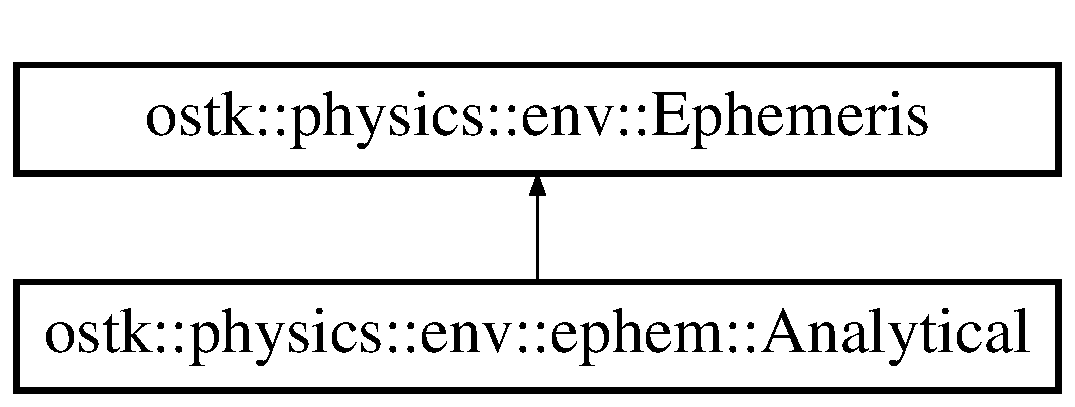
\includegraphics[height=2.000000cm]{classostk_1_1physics_1_1env_1_1ephem_1_1_analytical}
\end{center}
\end{figure}
\subsection*{Public Member Functions}
\begin{DoxyCompactItemize}
\item 
\hyperlink{classostk_1_1physics_1_1env_1_1ephem_1_1_analytical_a43cc9bb39be92ff42241c663e443ced3}{Analytical} (const Shared$<$ const \hyperlink{classostk_1_1physics_1_1coord_1_1_frame}{Frame} $>$ \&a\+Frame\+S\+Ptr)
\item 
virtual \hyperlink{classostk_1_1physics_1_1env_1_1ephem_1_1_analytical_a404523e0ada105dbf4bf54b3c1c91e05}{$\sim$\+Analytical} () override
\item 
virtual \hyperlink{classostk_1_1physics_1_1env_1_1ephem_1_1_analytical}{Analytical} $\ast$ \hyperlink{classostk_1_1physics_1_1env_1_1ephem_1_1_analytical_aeb01e31d1fd2d142efa5815ff3a44ea4}{clone} () const override
\item 
virtual bool \hyperlink{classostk_1_1physics_1_1env_1_1ephem_1_1_analytical_ac832a4552abfbeba38891cb936bc15ef}{is\+Defined} () const override
\item 
virtual Shared$<$ const \hyperlink{classostk_1_1physics_1_1coord_1_1_frame}{Frame} $>$ \hyperlink{classostk_1_1physics_1_1env_1_1ephem_1_1_analytical_a380712abe920ca25b2a3526d4a776033}{access\+Frame} () const override
\end{DoxyCompactItemize}


\subsection{Constructor \& Destructor Documentation}
\mbox{\Hypertarget{classostk_1_1physics_1_1env_1_1ephem_1_1_analytical_a43cc9bb39be92ff42241c663e443ced3}\label{classostk_1_1physics_1_1env_1_1ephem_1_1_analytical_a43cc9bb39be92ff42241c663e443ced3}} 
\index{ostk\+::physics\+::env\+::ephem\+::\+Analytical@{ostk\+::physics\+::env\+::ephem\+::\+Analytical}!Analytical@{Analytical}}
\index{Analytical@{Analytical}!ostk\+::physics\+::env\+::ephem\+::\+Analytical@{ostk\+::physics\+::env\+::ephem\+::\+Analytical}}
\subsubsection{\texorpdfstring{Analytical()}{Analytical()}}
{\footnotesize\ttfamily ostk\+::physics\+::env\+::ephem\+::\+Analytical\+::\+Analytical (\begin{DoxyParamCaption}\item[{const Shared$<$ const \hyperlink{classostk_1_1physics_1_1coord_1_1_frame}{Frame} $>$ \&}]{a\+Frame\+S\+Ptr }\end{DoxyParamCaption})}

\mbox{\Hypertarget{classostk_1_1physics_1_1env_1_1ephem_1_1_analytical_a404523e0ada105dbf4bf54b3c1c91e05}\label{classostk_1_1physics_1_1env_1_1ephem_1_1_analytical_a404523e0ada105dbf4bf54b3c1c91e05}} 
\index{ostk\+::physics\+::env\+::ephem\+::\+Analytical@{ostk\+::physics\+::env\+::ephem\+::\+Analytical}!````~Analytical@{$\sim$\+Analytical}}
\index{````~Analytical@{$\sim$\+Analytical}!ostk\+::physics\+::env\+::ephem\+::\+Analytical@{ostk\+::physics\+::env\+::ephem\+::\+Analytical}}
\subsubsection{\texorpdfstring{$\sim$\+Analytical()}{~Analytical()}}
{\footnotesize\ttfamily ostk\+::physics\+::env\+::ephem\+::\+Analytical\+::$\sim$\+Analytical (\begin{DoxyParamCaption}{ }\end{DoxyParamCaption})\hspace{0.3cm}{\ttfamily [override]}, {\ttfamily [virtual]}}



\subsection{Member Function Documentation}
\mbox{\Hypertarget{classostk_1_1physics_1_1env_1_1ephem_1_1_analytical_a380712abe920ca25b2a3526d4a776033}\label{classostk_1_1physics_1_1env_1_1ephem_1_1_analytical_a380712abe920ca25b2a3526d4a776033}} 
\index{ostk\+::physics\+::env\+::ephem\+::\+Analytical@{ostk\+::physics\+::env\+::ephem\+::\+Analytical}!access\+Frame@{access\+Frame}}
\index{access\+Frame@{access\+Frame}!ostk\+::physics\+::env\+::ephem\+::\+Analytical@{ostk\+::physics\+::env\+::ephem\+::\+Analytical}}
\subsubsection{\texorpdfstring{access\+Frame()}{accessFrame()}}
{\footnotesize\ttfamily Shared$<$ const \hyperlink{classostk_1_1physics_1_1coord_1_1_frame}{Frame} $>$ ostk\+::physics\+::env\+::ephem\+::\+Analytical\+::access\+Frame (\begin{DoxyParamCaption}{ }\end{DoxyParamCaption}) const\hspace{0.3cm}{\ttfamily [override]}, {\ttfamily [virtual]}}



Implements \hyperlink{classostk_1_1physics_1_1env_1_1_ephemeris_a7a2e78c90901d813311d51d66fcf12bf}{ostk\+::physics\+::env\+::\+Ephemeris}.

\mbox{\Hypertarget{classostk_1_1physics_1_1env_1_1ephem_1_1_analytical_aeb01e31d1fd2d142efa5815ff3a44ea4}\label{classostk_1_1physics_1_1env_1_1ephem_1_1_analytical_aeb01e31d1fd2d142efa5815ff3a44ea4}} 
\index{ostk\+::physics\+::env\+::ephem\+::\+Analytical@{ostk\+::physics\+::env\+::ephem\+::\+Analytical}!clone@{clone}}
\index{clone@{clone}!ostk\+::physics\+::env\+::ephem\+::\+Analytical@{ostk\+::physics\+::env\+::ephem\+::\+Analytical}}
\subsubsection{\texorpdfstring{clone()}{clone()}}
{\footnotesize\ttfamily \hyperlink{classostk_1_1physics_1_1env_1_1ephem_1_1_analytical}{Analytical} $\ast$ ostk\+::physics\+::env\+::ephem\+::\+Analytical\+::clone (\begin{DoxyParamCaption}{ }\end{DoxyParamCaption}) const\hspace{0.3cm}{\ttfamily [override]}, {\ttfamily [virtual]}}



Implements \hyperlink{classostk_1_1physics_1_1env_1_1_ephemeris_a3a35daaff1359882ae16b69ab6e399f6}{ostk\+::physics\+::env\+::\+Ephemeris}.

\mbox{\Hypertarget{classostk_1_1physics_1_1env_1_1ephem_1_1_analytical_ac832a4552abfbeba38891cb936bc15ef}\label{classostk_1_1physics_1_1env_1_1ephem_1_1_analytical_ac832a4552abfbeba38891cb936bc15ef}} 
\index{ostk\+::physics\+::env\+::ephem\+::\+Analytical@{ostk\+::physics\+::env\+::ephem\+::\+Analytical}!is\+Defined@{is\+Defined}}
\index{is\+Defined@{is\+Defined}!ostk\+::physics\+::env\+::ephem\+::\+Analytical@{ostk\+::physics\+::env\+::ephem\+::\+Analytical}}
\subsubsection{\texorpdfstring{is\+Defined()}{isDefined()}}
{\footnotesize\ttfamily bool ostk\+::physics\+::env\+::ephem\+::\+Analytical\+::is\+Defined (\begin{DoxyParamCaption}{ }\end{DoxyParamCaption}) const\hspace{0.3cm}{\ttfamily [override]}, {\ttfamily [virtual]}}



Implements \hyperlink{classostk_1_1physics_1_1env_1_1_ephemeris_ace5a637a5f25f700dfe1a2cef2b08162}{ostk\+::physics\+::env\+::\+Ephemeris}.



The documentation for this class was generated from the following files\+:\begin{DoxyCompactItemize}
\item 
include/\+Open\+Space\+Toolkit/\+Physics/\+Environment/\+Ephemerides/\hyperlink{_analytical_8hpp}{Analytical.\+hpp}\item 
src/\+Open\+Space\+Toolkit/\+Physics/\+Environment/\+Ephemerides/\hyperlink{_analytical_8cpp}{Analytical.\+cpp}\end{DoxyCompactItemize}

\hypertarget{classostk_1_1physics_1_1units_1_1_angle}{}\section{ostk\+:\+:physics\+:\+:units\+:\+:Angle Class Reference}
\label{classostk_1_1physics_1_1units_1_1_angle}\index{ostk\+::physics\+::units\+::\+Angle@{ostk\+::physics\+::units\+::\+Angle}}


\hyperlink{classostk_1_1physics_1_1units_1_1_angle}{Angle}.  




{\ttfamily \#include $<$Angle.\+hpp$>$}

Inheritance diagram for ostk\+:\+:physics\+:\+:units\+:\+:Angle\+:\begin{figure}[H]
\begin{center}
\leavevmode
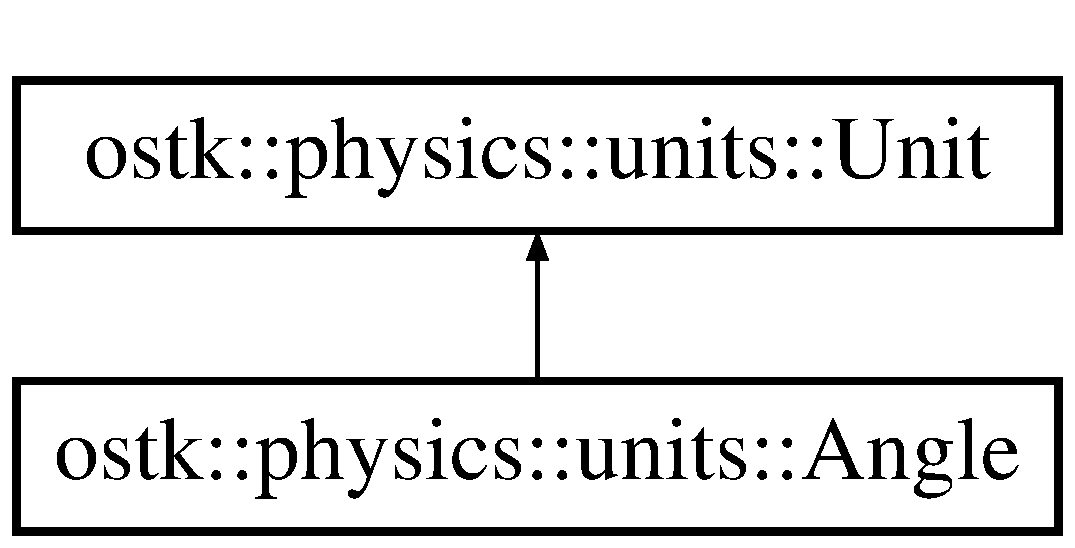
\includegraphics[height=2.000000cm]{classostk_1_1physics_1_1units_1_1_angle}
\end{center}
\end{figure}
\subsection*{Public Types}
\begin{DoxyCompactItemize}
\item 
enum \hyperlink{classostk_1_1physics_1_1units_1_1_angle_aea1f8018b1d378b9dee56959d8eb9def}{Unit} \{ \newline
\hyperlink{classostk_1_1physics_1_1units_1_1_angle_aea1f8018b1d378b9dee56959d8eb9defaec0fc0100c4fc1ce4eea230c3dc10360}{Unit\+::\+Undefined}, 
\hyperlink{classostk_1_1physics_1_1units_1_1_angle_aea1f8018b1d378b9dee56959d8eb9defa50c62e3ca8d8ec8732a7f968a3bf2c7c}{Unit\+::\+Radian}, 
\hyperlink{classostk_1_1physics_1_1units_1_1_angle_aea1f8018b1d378b9dee56959d8eb9defa6669c4dc00cb161446821b3529ca07d8}{Unit\+::\+Degree}, 
\hyperlink{classostk_1_1physics_1_1units_1_1_angle_aea1f8018b1d378b9dee56959d8eb9defa6d59f6ca1b5de72cbdc10a6792bcf090}{Unit\+::\+Arcminute}, 
\newline
\hyperlink{classostk_1_1physics_1_1units_1_1_angle_aea1f8018b1d378b9dee56959d8eb9defa7839ceecae19481f2e21e0ce3e11d3aa}{Unit\+::\+Arcsecond}, 
\hyperlink{classostk_1_1physics_1_1units_1_1_angle_aea1f8018b1d378b9dee56959d8eb9defaad09b2d48b2811c68e5a2bf421f7f2f2}{Unit\+::\+Revolution}
 \}
\end{DoxyCompactItemize}
\subsection*{Public Member Functions}
\begin{DoxyCompactItemize}
\item 
\hyperlink{classostk_1_1physics_1_1units_1_1_angle_a4892c7a7ed48adabf5c942dbda7ad848}{Angle} (const Real \&a\+Value, const \hyperlink{classostk_1_1physics_1_1units_1_1_angle_aea1f8018b1d378b9dee56959d8eb9def}{Angle\+::\+Unit} \&a\+Unit)
\begin{DoxyCompactList}\small\item\em Constructor. \end{DoxyCompactList}\item 
\hyperlink{classostk_1_1physics_1_1units_1_1_angle_a77a11a481467020f3bf965473dc37878}{Angle} (const ostk\+::math\+::geom\+::\+Angle \&an\+Angle)
\item 
virtual \hyperlink{classostk_1_1physics_1_1units_1_1_angle}{Angle} $\ast$ \hyperlink{classostk_1_1physics_1_1units_1_1_angle_af0d5d649b2a1310e6337663f7b9283bf}{clone} () const override
\item 
bool \hyperlink{classostk_1_1physics_1_1units_1_1_angle_a1199d17a4ea17dc976879f309a5e919f}{operator==} (const \hyperlink{classostk_1_1physics_1_1units_1_1_angle}{Angle} \&an\+Angle) const
\item 
bool \hyperlink{classostk_1_1physics_1_1units_1_1_angle_a7b920b7abe8e0fcc95a7a633f6240108}{operator!=} (const \hyperlink{classostk_1_1physics_1_1units_1_1_angle}{Angle} \&an\+Angle) const
\item 
\hyperlink{classostk_1_1physics_1_1units_1_1_angle}{Angle} \hyperlink{classostk_1_1physics_1_1units_1_1_angle_acbc8a13c8f84ed77a741538aa1d8ce91}{operator+} (const \hyperlink{classostk_1_1physics_1_1units_1_1_angle}{Angle} \&an\+Angle) const
\item 
\hyperlink{classostk_1_1physics_1_1units_1_1_angle}{Angle} \hyperlink{classostk_1_1physics_1_1units_1_1_angle_adc4e27520c40a157d3cf868b1df07c1c}{operator-\/} (const \hyperlink{classostk_1_1physics_1_1units_1_1_angle}{Angle} \&an\+Angle) const
\item 
\hyperlink{classostk_1_1physics_1_1units_1_1_angle}{Angle} \hyperlink{classostk_1_1physics_1_1units_1_1_angle_abd90998581807fadf43720f558061115}{operator$\ast$} (const Real \&a\+Real) const
\item 
\hyperlink{classostk_1_1physics_1_1units_1_1_angle}{Angle} \hyperlink{classostk_1_1physics_1_1units_1_1_angle_a5507ed91abc944fd4cc91f5488276e95}{operator/} (const Real \&a\+Real) const
\item 
\hyperlink{classostk_1_1physics_1_1units_1_1_angle}{Angle} \& \hyperlink{classostk_1_1physics_1_1units_1_1_angle_a814933d09dc8cb6cb4a7a013386c2267}{operator+=} (const \hyperlink{classostk_1_1physics_1_1units_1_1_angle}{Angle} \&an\+Angle)
\item 
\hyperlink{classostk_1_1physics_1_1units_1_1_angle}{Angle} \& \hyperlink{classostk_1_1physics_1_1units_1_1_angle_ac7699382075d4997670ed0071f8ba540}{operator-\/=} (const \hyperlink{classostk_1_1physics_1_1units_1_1_angle}{Angle} \&an\+Angle)
\item 
\hyperlink{classostk_1_1physics_1_1units_1_1_angle}{Angle} \& \hyperlink{classostk_1_1physics_1_1units_1_1_angle_aba01c2eb2166f1be5c5ff8d5b2cb6363}{operator$\ast$=} (const Real \&a\+Real)
\item 
\hyperlink{classostk_1_1physics_1_1units_1_1_angle}{Angle} \& \hyperlink{classostk_1_1physics_1_1units_1_1_angle_aaa0ad11b6d769a44c3a5bcef2bad8b6a}{operator/=} (const Real \&a\+Real)
\item 
\hyperlink{classostk_1_1physics_1_1units_1_1_angle_ae92c124ae780a2c61747f343a6b3f773}{operator ostk\+::math\+::geom\+::\+Angle} () const
\item 
virtual bool \hyperlink{classostk_1_1physics_1_1units_1_1_angle_a912562d12513b2fcee56262208206b62}{is\+Defined} () const override
\item 
\hyperlink{classostk_1_1physics_1_1units_1_1_angle_aea1f8018b1d378b9dee56959d8eb9def}{Angle\+::\+Unit} \hyperlink{classostk_1_1physics_1_1units_1_1_angle_abe7e90d80d24d15464a6041569196ea3}{get\+Unit} () const
\item 
Real \hyperlink{classostk_1_1physics_1_1units_1_1_angle_a80e7aa75986fc9b4644b6d0db4f3ba9c}{in} (const \hyperlink{classostk_1_1physics_1_1units_1_1_angle_aea1f8018b1d378b9dee56959d8eb9def}{Angle\+::\+Unit} \&a\+Unit) const
\item 
Real \hyperlink{classostk_1_1physics_1_1units_1_1_angle_a732c6410b7eae97dadec4c9151c86e3b}{in\+Radians} () const
\item 
Real \hyperlink{classostk_1_1physics_1_1units_1_1_angle_acaa7d6b9b7ff74854c194b554cfe94a6}{in\+Radians} (const Real \&a\+Lower\+Bound, const Real \&an\+Upper\+Bound) const
\item 
Real \hyperlink{classostk_1_1physics_1_1units_1_1_angle_ac5faeae2943418bfebdf26a641083662}{in\+Degrees} () const
\item 
Real \hyperlink{classostk_1_1physics_1_1units_1_1_angle_aa1ea48dcf3d6c11fb6317f422604a382}{in\+Degrees} (const Real \&a\+Lower\+Bound, const Real \&an\+Upper\+Bound) const
\item 
Real \hyperlink{classostk_1_1physics_1_1units_1_1_angle_a03d9c3a133d4076b6a67a0abc8d73271}{in\+Arcminutes} () const
\item 
Real \hyperlink{classostk_1_1physics_1_1units_1_1_angle_a678a42204ee95b335e30853d94b31689}{in\+Arcminutes} (const Real \&a\+Lower\+Bound, const Real \&an\+Upper\+Bound) const
\item 
Real \hyperlink{classostk_1_1physics_1_1units_1_1_angle_ae1898d207b9a0a54bec27a4abfa30db7}{in\+Arcseconds} () const
\item 
Real \hyperlink{classostk_1_1physics_1_1units_1_1_angle_a6ccbfdaeeda6aa1bb812d9bef768fb84}{in\+Arcseconds} (const Real \&a\+Lower\+Bound, const Real \&an\+Upper\+Bound) const
\item 
Real \hyperlink{classostk_1_1physics_1_1units_1_1_angle_a8e0d12ccfb07c08113f9f183272344c8}{in\+Revolutions} () const
\item 
virtual String \hyperlink{classostk_1_1physics_1_1units_1_1_angle_a7403146e01d293dfdd30130f9a9f0f2f}{to\+String} (const Integer \&a\+Precision=Integer\+::\+Undefined()) const override
\end{DoxyCompactItemize}
\subsection*{Static Public Member Functions}
\begin{DoxyCompactItemize}
\item 
static \hyperlink{classostk_1_1physics_1_1units_1_1_angle}{Angle} \hyperlink{classostk_1_1physics_1_1units_1_1_angle_abfde70c3cfb9fa966ee91d498092766a}{Undefined} ()
\item 
static \hyperlink{classostk_1_1physics_1_1units_1_1_angle}{Angle} \hyperlink{classostk_1_1physics_1_1units_1_1_angle_a4454975f87e5d3532cf8b819819207e7}{Zero} ()
\item 
static \hyperlink{classostk_1_1physics_1_1units_1_1_angle}{Angle} \hyperlink{classostk_1_1physics_1_1units_1_1_angle_a6065318d10aee4f99d28af429a64d9bb}{Half\+Pi} ()
\item 
static \hyperlink{classostk_1_1physics_1_1units_1_1_angle}{Angle} \hyperlink{classostk_1_1physics_1_1units_1_1_angle_ad207d164950a07ee779a199d5c4765c1}{Pi} ()
\item 
static \hyperlink{classostk_1_1physics_1_1units_1_1_angle}{Angle} \hyperlink{classostk_1_1physics_1_1units_1_1_angle_a2a78cc568975aa82e2011e24cd015f72}{Two\+Pi} ()
\item 
static \hyperlink{classostk_1_1physics_1_1units_1_1_angle}{Angle} \hyperlink{classostk_1_1physics_1_1units_1_1_angle_aceb137f392490d9b1d1de90406e62c9c}{Radians} (const Real \&a\+Value)
\item 
static \hyperlink{classostk_1_1physics_1_1units_1_1_angle}{Angle} \hyperlink{classostk_1_1physics_1_1units_1_1_angle_a6cddbceb5fd1f0c2a6dd29dae047baee}{Degrees} (const Real \&a\+Value)
\item 
static \hyperlink{classostk_1_1physics_1_1units_1_1_angle}{Angle} \hyperlink{classostk_1_1physics_1_1units_1_1_angle_a1cd6da5abf0593c2c3f3b4908c3c7008}{Arcminutes} (const Real \&a\+Value)
\item 
static \hyperlink{classostk_1_1physics_1_1units_1_1_angle}{Angle} \hyperlink{classostk_1_1physics_1_1units_1_1_angle_ac5817629ffd63aa9df93f0ee8b61af3a}{Arcseconds} (const Real \&a\+Value)
\item 
static \hyperlink{classostk_1_1physics_1_1units_1_1_angle}{Angle} \hyperlink{classostk_1_1physics_1_1units_1_1_angle_a827dcc99310b0b0117cf5d7dd5b4c899}{Revolutions} (const Real \&a\+Value)
\item 
static \hyperlink{classostk_1_1physics_1_1units_1_1_angle}{Angle} \hyperlink{classostk_1_1physics_1_1units_1_1_angle_a49c63c044fe667b0c210c6cd5b881380}{Between} (const Vector2d \&a\+First\+Vector, const Vector2d \&a\+Second\+Vector)
\item 
static \hyperlink{classostk_1_1physics_1_1units_1_1_angle}{Angle} \hyperlink{classostk_1_1physics_1_1units_1_1_angle_a7795cc65081205ece71c45b846729ad5}{Between} (const Vector3d \&a\+First\+Vector, const Vector3d \&a\+Second\+Vector)
\item 
static \hyperlink{classostk_1_1physics_1_1units_1_1_angle}{Angle} \hyperlink{classostk_1_1physics_1_1units_1_1_angle_a13d4a4ef4fc8c44f9f3aaf6c191a9451}{Parse} (const String \&a\+String)
\item 
static String \hyperlink{classostk_1_1physics_1_1units_1_1_angle_ad4b96eb55989dd56a8b730157d51c220}{String\+From\+Unit} (const \hyperlink{classostk_1_1physics_1_1units_1_1_angle_aea1f8018b1d378b9dee56959d8eb9def}{Angle\+::\+Unit} \&a\+Unit)
\item 
static String \hyperlink{classostk_1_1physics_1_1units_1_1_angle_a8368ccc4f26856471d22134d9a6fb0d2}{Symbol\+From\+Unit} (const \hyperlink{classostk_1_1physics_1_1units_1_1_angle_aea1f8018b1d378b9dee56959d8eb9def}{Angle\+::\+Unit} \&a\+Unit)
\item 
static \hyperlink{classostk_1_1physics_1_1units_1_1_angle_aea1f8018b1d378b9dee56959d8eb9def}{Angle\+::\+Unit} \hyperlink{classostk_1_1physics_1_1units_1_1_angle_a754e7c95f024bc77fa69c58b0d02fd87}{Unit\+From\+Symbol} (const String \&a\+Symbol)
\end{DoxyCompactItemize}
\subsection*{Friends}
\begin{DoxyCompactItemize}
\item 
\hyperlink{classostk_1_1physics_1_1units_1_1_angle}{Angle} \hyperlink{classostk_1_1physics_1_1units_1_1_angle_af699984b24759466957ecddaa7e61fc9}{operator$\ast$} (const Real \&a\+Real, const \hyperlink{classostk_1_1physics_1_1units_1_1_angle}{Angle} \&an\+Angle)
\item 
std\+::ostream \& \hyperlink{classostk_1_1physics_1_1units_1_1_angle_a0846b77ee3281e8a559197c3c3208eed}{operator$<$$<$} (std\+::ostream \&an\+Output\+Stream, const \hyperlink{classostk_1_1physics_1_1units_1_1_angle}{Angle} \&an\+Angle)
\end{DoxyCompactItemize}
\subsection*{Additional Inherited Members}


\subsection{Detailed Description}
\hyperlink{classostk_1_1physics_1_1units_1_1_angle}{Angle}. 

In plane geometry, an angle is the figure formed by two rays, called the sides of the angle, sharing a common endpoint, called the vertex of the angle.

https\+://en.wikipedia.\+org/wiki/\+Angle 

\subsection{Member Enumeration Documentation}
\mbox{\Hypertarget{classostk_1_1physics_1_1units_1_1_angle_aea1f8018b1d378b9dee56959d8eb9def}\label{classostk_1_1physics_1_1units_1_1_angle_aea1f8018b1d378b9dee56959d8eb9def}} 
\index{ostk\+::physics\+::units\+::\+Angle@{ostk\+::physics\+::units\+::\+Angle}!Unit@{Unit}}
\index{Unit@{Unit}!ostk\+::physics\+::units\+::\+Angle@{ostk\+::physics\+::units\+::\+Angle}}
\subsubsection{\texorpdfstring{Unit}{Unit}}
{\footnotesize\ttfamily enum \hyperlink{classostk_1_1physics_1_1units_1_1_angle_aea1f8018b1d378b9dee56959d8eb9def}{ostk\+::physics\+::units\+::\+Angle\+::\+Unit}\hspace{0.3cm}{\ttfamily [strong]}}

\begin{DoxyEnumFields}{Enumerator}
\raisebox{\heightof{T}}[0pt][0pt]{\index{Undefined@{Undefined}!ostk\+::physics\+::units\+::\+Angle@{ostk\+::physics\+::units\+::\+Angle}}\index{ostk\+::physics\+::units\+::\+Angle@{ostk\+::physics\+::units\+::\+Angle}!Undefined@{Undefined}}}\mbox{\Hypertarget{classostk_1_1physics_1_1units_1_1_angle_aea1f8018b1d378b9dee56959d8eb9defaec0fc0100c4fc1ce4eea230c3dc10360}\label{classostk_1_1physics_1_1units_1_1_angle_aea1f8018b1d378b9dee56959d8eb9defaec0fc0100c4fc1ce4eea230c3dc10360}} 
Undefined&Undefined. \\
\hline

\raisebox{\heightof{T}}[0pt][0pt]{\index{Radian@{Radian}!ostk\+::physics\+::units\+::\+Angle@{ostk\+::physics\+::units\+::\+Angle}}\index{ostk\+::physics\+::units\+::\+Angle@{ostk\+::physics\+::units\+::\+Angle}!Radian@{Radian}}}\mbox{\Hypertarget{classostk_1_1physics_1_1units_1_1_angle_aea1f8018b1d378b9dee56959d8eb9defa50c62e3ca8d8ec8732a7f968a3bf2c7c}\label{classostk_1_1physics_1_1units_1_1_angle_aea1f8018b1d378b9dee56959d8eb9defa50c62e3ca8d8ec8732a7f968a3bf2c7c}} 
Radian&Radian. \\
\hline

\raisebox{\heightof{T}}[0pt][0pt]{\index{Degree@{Degree}!ostk\+::physics\+::units\+::\+Angle@{ostk\+::physics\+::units\+::\+Angle}}\index{ostk\+::physics\+::units\+::\+Angle@{ostk\+::physics\+::units\+::\+Angle}!Degree@{Degree}}}\mbox{\Hypertarget{classostk_1_1physics_1_1units_1_1_angle_aea1f8018b1d378b9dee56959d8eb9defa6669c4dc00cb161446821b3529ca07d8}\label{classostk_1_1physics_1_1units_1_1_angle_aea1f8018b1d378b9dee56959d8eb9defa6669c4dc00cb161446821b3529ca07d8}} 
Degree&Degree. \\
\hline

\raisebox{\heightof{T}}[0pt][0pt]{\index{Arcminute@{Arcminute}!ostk\+::physics\+::units\+::\+Angle@{ostk\+::physics\+::units\+::\+Angle}}\index{ostk\+::physics\+::units\+::\+Angle@{ostk\+::physics\+::units\+::\+Angle}!Arcminute@{Arcminute}}}\mbox{\Hypertarget{classostk_1_1physics_1_1units_1_1_angle_aea1f8018b1d378b9dee56959d8eb9defa6d59f6ca1b5de72cbdc10a6792bcf090}\label{classostk_1_1physics_1_1units_1_1_angle_aea1f8018b1d378b9dee56959d8eb9defa6d59f6ca1b5de72cbdc10a6792bcf090}} 
Arcminute&Arcminute. \\
\hline

\raisebox{\heightof{T}}[0pt][0pt]{\index{Arcsecond@{Arcsecond}!ostk\+::physics\+::units\+::\+Angle@{ostk\+::physics\+::units\+::\+Angle}}\index{ostk\+::physics\+::units\+::\+Angle@{ostk\+::physics\+::units\+::\+Angle}!Arcsecond@{Arcsecond}}}\mbox{\Hypertarget{classostk_1_1physics_1_1units_1_1_angle_aea1f8018b1d378b9dee56959d8eb9defa7839ceecae19481f2e21e0ce3e11d3aa}\label{classostk_1_1physics_1_1units_1_1_angle_aea1f8018b1d378b9dee56959d8eb9defa7839ceecae19481f2e21e0ce3e11d3aa}} 
Arcsecond&Arcsecond. \\
\hline

\raisebox{\heightof{T}}[0pt][0pt]{\index{Revolution@{Revolution}!ostk\+::physics\+::units\+::\+Angle@{ostk\+::physics\+::units\+::\+Angle}}\index{ostk\+::physics\+::units\+::\+Angle@{ostk\+::physics\+::units\+::\+Angle}!Revolution@{Revolution}}}\mbox{\Hypertarget{classostk_1_1physics_1_1units_1_1_angle_aea1f8018b1d378b9dee56959d8eb9defaad09b2d48b2811c68e5a2bf421f7f2f2}\label{classostk_1_1physics_1_1units_1_1_angle_aea1f8018b1d378b9dee56959d8eb9defaad09b2d48b2811c68e5a2bf421f7f2f2}} 
Revolution&Revolution. \\
\hline

\end{DoxyEnumFields}


\subsection{Constructor \& Destructor Documentation}
\mbox{\Hypertarget{classostk_1_1physics_1_1units_1_1_angle_a4892c7a7ed48adabf5c942dbda7ad848}\label{classostk_1_1physics_1_1units_1_1_angle_a4892c7a7ed48adabf5c942dbda7ad848}} 
\index{ostk\+::physics\+::units\+::\+Angle@{ostk\+::physics\+::units\+::\+Angle}!Angle@{Angle}}
\index{Angle@{Angle}!ostk\+::physics\+::units\+::\+Angle@{ostk\+::physics\+::units\+::\+Angle}}
\subsubsection{\texorpdfstring{Angle()}{Angle()}\hspace{0.1cm}{\footnotesize\ttfamily [1/2]}}
{\footnotesize\ttfamily ostk\+::physics\+::units\+::\+Angle\+::\+Angle (\begin{DoxyParamCaption}\item[{const Real \&}]{a\+Value,  }\item[{const \hyperlink{classostk_1_1physics_1_1units_1_1_angle_aea1f8018b1d378b9dee56959d8eb9def}{Angle\+::\+Unit} \&}]{a\+Unit }\end{DoxyParamCaption})}



Constructor. 


\begin{DoxyCode}
\hyperlink{classostk_1_1physics_1_1units_1_1_angle_a4892c7a7ed48adabf5c942dbda7ad848}{Angle} angle(90.0, \hyperlink{classostk_1_1physics_1_1units_1_1_angle_aea1f8018b1d378b9dee56959d8eb9defa6669c4dc00cb161446821b3529ca07d8}{Angle::Unit::Degree}) ;
\end{DoxyCode}



\begin{DoxyParams}[1]{Parameters}
\mbox{\tt in}  & {\em a\+Value} & A value \\
\hline
\mbox{\tt in}  & {\em a\+Unit} & An angle unit \\
\hline
\end{DoxyParams}
\mbox{\Hypertarget{classostk_1_1physics_1_1units_1_1_angle_a77a11a481467020f3bf965473dc37878}\label{classostk_1_1physics_1_1units_1_1_angle_a77a11a481467020f3bf965473dc37878}} 
\index{ostk\+::physics\+::units\+::\+Angle@{ostk\+::physics\+::units\+::\+Angle}!Angle@{Angle}}
\index{Angle@{Angle}!ostk\+::physics\+::units\+::\+Angle@{ostk\+::physics\+::units\+::\+Angle}}
\subsubsection{\texorpdfstring{Angle()}{Angle()}\hspace{0.1cm}{\footnotesize\ttfamily [2/2]}}
{\footnotesize\ttfamily ostk\+::physics\+::units\+::\+Angle\+::\+Angle (\begin{DoxyParamCaption}\item[{const ostk\+::math\+::geom\+::\+Angle \&}]{an\+Angle }\end{DoxyParamCaption})}



\subsection{Member Function Documentation}
\mbox{\Hypertarget{classostk_1_1physics_1_1units_1_1_angle_a1cd6da5abf0593c2c3f3b4908c3c7008}\label{classostk_1_1physics_1_1units_1_1_angle_a1cd6da5abf0593c2c3f3b4908c3c7008}} 
\index{ostk\+::physics\+::units\+::\+Angle@{ostk\+::physics\+::units\+::\+Angle}!Arcminutes@{Arcminutes}}
\index{Arcminutes@{Arcminutes}!ostk\+::physics\+::units\+::\+Angle@{ostk\+::physics\+::units\+::\+Angle}}
\subsubsection{\texorpdfstring{Arcminutes()}{Arcminutes()}}
{\footnotesize\ttfamily \hyperlink{classostk_1_1physics_1_1units_1_1_angle}{Angle} ostk\+::physics\+::units\+::\+Angle\+::\+Arcminutes (\begin{DoxyParamCaption}\item[{const Real \&}]{a\+Value }\end{DoxyParamCaption})\hspace{0.3cm}{\ttfamily [static]}}

\mbox{\Hypertarget{classostk_1_1physics_1_1units_1_1_angle_ac5817629ffd63aa9df93f0ee8b61af3a}\label{classostk_1_1physics_1_1units_1_1_angle_ac5817629ffd63aa9df93f0ee8b61af3a}} 
\index{ostk\+::physics\+::units\+::\+Angle@{ostk\+::physics\+::units\+::\+Angle}!Arcseconds@{Arcseconds}}
\index{Arcseconds@{Arcseconds}!ostk\+::physics\+::units\+::\+Angle@{ostk\+::physics\+::units\+::\+Angle}}
\subsubsection{\texorpdfstring{Arcseconds()}{Arcseconds()}}
{\footnotesize\ttfamily \hyperlink{classostk_1_1physics_1_1units_1_1_angle}{Angle} ostk\+::physics\+::units\+::\+Angle\+::\+Arcseconds (\begin{DoxyParamCaption}\item[{const Real \&}]{a\+Value }\end{DoxyParamCaption})\hspace{0.3cm}{\ttfamily [static]}}

\mbox{\Hypertarget{classostk_1_1physics_1_1units_1_1_angle_a49c63c044fe667b0c210c6cd5b881380}\label{classostk_1_1physics_1_1units_1_1_angle_a49c63c044fe667b0c210c6cd5b881380}} 
\index{ostk\+::physics\+::units\+::\+Angle@{ostk\+::physics\+::units\+::\+Angle}!Between@{Between}}
\index{Between@{Between}!ostk\+::physics\+::units\+::\+Angle@{ostk\+::physics\+::units\+::\+Angle}}
\subsubsection{\texorpdfstring{Between()}{Between()}\hspace{0.1cm}{\footnotesize\ttfamily [1/2]}}
{\footnotesize\ttfamily \hyperlink{classostk_1_1physics_1_1units_1_1_angle}{Angle} ostk\+::physics\+::units\+::\+Angle\+::\+Between (\begin{DoxyParamCaption}\item[{const Vector2d \&}]{a\+First\+Vector,  }\item[{const Vector2d \&}]{a\+Second\+Vector }\end{DoxyParamCaption})\hspace{0.3cm}{\ttfamily [static]}}

\mbox{\Hypertarget{classostk_1_1physics_1_1units_1_1_angle_a7795cc65081205ece71c45b846729ad5}\label{classostk_1_1physics_1_1units_1_1_angle_a7795cc65081205ece71c45b846729ad5}} 
\index{ostk\+::physics\+::units\+::\+Angle@{ostk\+::physics\+::units\+::\+Angle}!Between@{Between}}
\index{Between@{Between}!ostk\+::physics\+::units\+::\+Angle@{ostk\+::physics\+::units\+::\+Angle}}
\subsubsection{\texorpdfstring{Between()}{Between()}\hspace{0.1cm}{\footnotesize\ttfamily [2/2]}}
{\footnotesize\ttfamily \hyperlink{classostk_1_1physics_1_1units_1_1_angle}{Angle} ostk\+::physics\+::units\+::\+Angle\+::\+Between (\begin{DoxyParamCaption}\item[{const Vector3d \&}]{a\+First\+Vector,  }\item[{const Vector3d \&}]{a\+Second\+Vector }\end{DoxyParamCaption})\hspace{0.3cm}{\ttfamily [static]}}

\mbox{\Hypertarget{classostk_1_1physics_1_1units_1_1_angle_af0d5d649b2a1310e6337663f7b9283bf}\label{classostk_1_1physics_1_1units_1_1_angle_af0d5d649b2a1310e6337663f7b9283bf}} 
\index{ostk\+::physics\+::units\+::\+Angle@{ostk\+::physics\+::units\+::\+Angle}!clone@{clone}}
\index{clone@{clone}!ostk\+::physics\+::units\+::\+Angle@{ostk\+::physics\+::units\+::\+Angle}}
\subsubsection{\texorpdfstring{clone()}{clone()}}
{\footnotesize\ttfamily \hyperlink{classostk_1_1physics_1_1units_1_1_angle}{Angle} $\ast$ ostk\+::physics\+::units\+::\+Angle\+::clone (\begin{DoxyParamCaption}{ }\end{DoxyParamCaption}) const\hspace{0.3cm}{\ttfamily [override]}, {\ttfamily [virtual]}}



Implements \hyperlink{classostk_1_1physics_1_1units_1_1_unit_ab203628f8a16b16c28d89eaa4c3aff67}{ostk\+::physics\+::units\+::\+Unit}.

\mbox{\Hypertarget{classostk_1_1physics_1_1units_1_1_angle_a6cddbceb5fd1f0c2a6dd29dae047baee}\label{classostk_1_1physics_1_1units_1_1_angle_a6cddbceb5fd1f0c2a6dd29dae047baee}} 
\index{ostk\+::physics\+::units\+::\+Angle@{ostk\+::physics\+::units\+::\+Angle}!Degrees@{Degrees}}
\index{Degrees@{Degrees}!ostk\+::physics\+::units\+::\+Angle@{ostk\+::physics\+::units\+::\+Angle}}
\subsubsection{\texorpdfstring{Degrees()}{Degrees()}}
{\footnotesize\ttfamily \hyperlink{classostk_1_1physics_1_1units_1_1_angle}{Angle} ostk\+::physics\+::units\+::\+Angle\+::\+Degrees (\begin{DoxyParamCaption}\item[{const Real \&}]{a\+Value }\end{DoxyParamCaption})\hspace{0.3cm}{\ttfamily [static]}}

\mbox{\Hypertarget{classostk_1_1physics_1_1units_1_1_angle_abe7e90d80d24d15464a6041569196ea3}\label{classostk_1_1physics_1_1units_1_1_angle_abe7e90d80d24d15464a6041569196ea3}} 
\index{ostk\+::physics\+::units\+::\+Angle@{ostk\+::physics\+::units\+::\+Angle}!get\+Unit@{get\+Unit}}
\index{get\+Unit@{get\+Unit}!ostk\+::physics\+::units\+::\+Angle@{ostk\+::physics\+::units\+::\+Angle}}
\subsubsection{\texorpdfstring{get\+Unit()}{getUnit()}}
{\footnotesize\ttfamily \hyperlink{classostk_1_1physics_1_1units_1_1_angle_aea1f8018b1d378b9dee56959d8eb9def}{Angle\+::\+Unit} ostk\+::physics\+::units\+::\+Angle\+::get\+Unit (\begin{DoxyParamCaption}{ }\end{DoxyParamCaption}) const}

\mbox{\Hypertarget{classostk_1_1physics_1_1units_1_1_angle_a6065318d10aee4f99d28af429a64d9bb}\label{classostk_1_1physics_1_1units_1_1_angle_a6065318d10aee4f99d28af429a64d9bb}} 
\index{ostk\+::physics\+::units\+::\+Angle@{ostk\+::physics\+::units\+::\+Angle}!Half\+Pi@{Half\+Pi}}
\index{Half\+Pi@{Half\+Pi}!ostk\+::physics\+::units\+::\+Angle@{ostk\+::physics\+::units\+::\+Angle}}
\subsubsection{\texorpdfstring{Half\+Pi()}{HalfPi()}}
{\footnotesize\ttfamily \hyperlink{classostk_1_1physics_1_1units_1_1_angle}{Angle} ostk\+::physics\+::units\+::\+Angle\+::\+Half\+Pi (\begin{DoxyParamCaption}{ }\end{DoxyParamCaption})\hspace{0.3cm}{\ttfamily [static]}}

\mbox{\Hypertarget{classostk_1_1physics_1_1units_1_1_angle_a80e7aa75986fc9b4644b6d0db4f3ba9c}\label{classostk_1_1physics_1_1units_1_1_angle_a80e7aa75986fc9b4644b6d0db4f3ba9c}} 
\index{ostk\+::physics\+::units\+::\+Angle@{ostk\+::physics\+::units\+::\+Angle}!in@{in}}
\index{in@{in}!ostk\+::physics\+::units\+::\+Angle@{ostk\+::physics\+::units\+::\+Angle}}
\subsubsection{\texorpdfstring{in()}{in()}}
{\footnotesize\ttfamily Real ostk\+::physics\+::units\+::\+Angle\+::in (\begin{DoxyParamCaption}\item[{const \hyperlink{classostk_1_1physics_1_1units_1_1_angle_aea1f8018b1d378b9dee56959d8eb9def}{Angle\+::\+Unit} \&}]{a\+Unit }\end{DoxyParamCaption}) const}

\mbox{\Hypertarget{classostk_1_1physics_1_1units_1_1_angle_a03d9c3a133d4076b6a67a0abc8d73271}\label{classostk_1_1physics_1_1units_1_1_angle_a03d9c3a133d4076b6a67a0abc8d73271}} 
\index{ostk\+::physics\+::units\+::\+Angle@{ostk\+::physics\+::units\+::\+Angle}!in\+Arcminutes@{in\+Arcminutes}}
\index{in\+Arcminutes@{in\+Arcminutes}!ostk\+::physics\+::units\+::\+Angle@{ostk\+::physics\+::units\+::\+Angle}}
\subsubsection{\texorpdfstring{in\+Arcminutes()}{inArcminutes()}\hspace{0.1cm}{\footnotesize\ttfamily [1/2]}}
{\footnotesize\ttfamily Real ostk\+::physics\+::units\+::\+Angle\+::in\+Arcminutes (\begin{DoxyParamCaption}{ }\end{DoxyParamCaption}) const}

\mbox{\Hypertarget{classostk_1_1physics_1_1units_1_1_angle_a678a42204ee95b335e30853d94b31689}\label{classostk_1_1physics_1_1units_1_1_angle_a678a42204ee95b335e30853d94b31689}} 
\index{ostk\+::physics\+::units\+::\+Angle@{ostk\+::physics\+::units\+::\+Angle}!in\+Arcminutes@{in\+Arcminutes}}
\index{in\+Arcminutes@{in\+Arcminutes}!ostk\+::physics\+::units\+::\+Angle@{ostk\+::physics\+::units\+::\+Angle}}
\subsubsection{\texorpdfstring{in\+Arcminutes()}{inArcminutes()}\hspace{0.1cm}{\footnotesize\ttfamily [2/2]}}
{\footnotesize\ttfamily Real ostk\+::physics\+::units\+::\+Angle\+::in\+Arcminutes (\begin{DoxyParamCaption}\item[{const Real \&}]{a\+Lower\+Bound,  }\item[{const Real \&}]{an\+Upper\+Bound }\end{DoxyParamCaption}) const}

\mbox{\Hypertarget{classostk_1_1physics_1_1units_1_1_angle_ae1898d207b9a0a54bec27a4abfa30db7}\label{classostk_1_1physics_1_1units_1_1_angle_ae1898d207b9a0a54bec27a4abfa30db7}} 
\index{ostk\+::physics\+::units\+::\+Angle@{ostk\+::physics\+::units\+::\+Angle}!in\+Arcseconds@{in\+Arcseconds}}
\index{in\+Arcseconds@{in\+Arcseconds}!ostk\+::physics\+::units\+::\+Angle@{ostk\+::physics\+::units\+::\+Angle}}
\subsubsection{\texorpdfstring{in\+Arcseconds()}{inArcseconds()}\hspace{0.1cm}{\footnotesize\ttfamily [1/2]}}
{\footnotesize\ttfamily Real ostk\+::physics\+::units\+::\+Angle\+::in\+Arcseconds (\begin{DoxyParamCaption}{ }\end{DoxyParamCaption}) const}

\mbox{\Hypertarget{classostk_1_1physics_1_1units_1_1_angle_a6ccbfdaeeda6aa1bb812d9bef768fb84}\label{classostk_1_1physics_1_1units_1_1_angle_a6ccbfdaeeda6aa1bb812d9bef768fb84}} 
\index{ostk\+::physics\+::units\+::\+Angle@{ostk\+::physics\+::units\+::\+Angle}!in\+Arcseconds@{in\+Arcseconds}}
\index{in\+Arcseconds@{in\+Arcseconds}!ostk\+::physics\+::units\+::\+Angle@{ostk\+::physics\+::units\+::\+Angle}}
\subsubsection{\texorpdfstring{in\+Arcseconds()}{inArcseconds()}\hspace{0.1cm}{\footnotesize\ttfamily [2/2]}}
{\footnotesize\ttfamily Real ostk\+::physics\+::units\+::\+Angle\+::in\+Arcseconds (\begin{DoxyParamCaption}\item[{const Real \&}]{a\+Lower\+Bound,  }\item[{const Real \&}]{an\+Upper\+Bound }\end{DoxyParamCaption}) const}

\mbox{\Hypertarget{classostk_1_1physics_1_1units_1_1_angle_ac5faeae2943418bfebdf26a641083662}\label{classostk_1_1physics_1_1units_1_1_angle_ac5faeae2943418bfebdf26a641083662}} 
\index{ostk\+::physics\+::units\+::\+Angle@{ostk\+::physics\+::units\+::\+Angle}!in\+Degrees@{in\+Degrees}}
\index{in\+Degrees@{in\+Degrees}!ostk\+::physics\+::units\+::\+Angle@{ostk\+::physics\+::units\+::\+Angle}}
\subsubsection{\texorpdfstring{in\+Degrees()}{inDegrees()}\hspace{0.1cm}{\footnotesize\ttfamily [1/2]}}
{\footnotesize\ttfamily Real ostk\+::physics\+::units\+::\+Angle\+::in\+Degrees (\begin{DoxyParamCaption}{ }\end{DoxyParamCaption}) const}

\mbox{\Hypertarget{classostk_1_1physics_1_1units_1_1_angle_aa1ea48dcf3d6c11fb6317f422604a382}\label{classostk_1_1physics_1_1units_1_1_angle_aa1ea48dcf3d6c11fb6317f422604a382}} 
\index{ostk\+::physics\+::units\+::\+Angle@{ostk\+::physics\+::units\+::\+Angle}!in\+Degrees@{in\+Degrees}}
\index{in\+Degrees@{in\+Degrees}!ostk\+::physics\+::units\+::\+Angle@{ostk\+::physics\+::units\+::\+Angle}}
\subsubsection{\texorpdfstring{in\+Degrees()}{inDegrees()}\hspace{0.1cm}{\footnotesize\ttfamily [2/2]}}
{\footnotesize\ttfamily Real ostk\+::physics\+::units\+::\+Angle\+::in\+Degrees (\begin{DoxyParamCaption}\item[{const Real \&}]{a\+Lower\+Bound,  }\item[{const Real \&}]{an\+Upper\+Bound }\end{DoxyParamCaption}) const}

\mbox{\Hypertarget{classostk_1_1physics_1_1units_1_1_angle_a732c6410b7eae97dadec4c9151c86e3b}\label{classostk_1_1physics_1_1units_1_1_angle_a732c6410b7eae97dadec4c9151c86e3b}} 
\index{ostk\+::physics\+::units\+::\+Angle@{ostk\+::physics\+::units\+::\+Angle}!in\+Radians@{in\+Radians}}
\index{in\+Radians@{in\+Radians}!ostk\+::physics\+::units\+::\+Angle@{ostk\+::physics\+::units\+::\+Angle}}
\subsubsection{\texorpdfstring{in\+Radians()}{inRadians()}\hspace{0.1cm}{\footnotesize\ttfamily [1/2]}}
{\footnotesize\ttfamily Real ostk\+::physics\+::units\+::\+Angle\+::in\+Radians (\begin{DoxyParamCaption}{ }\end{DoxyParamCaption}) const}

\mbox{\Hypertarget{classostk_1_1physics_1_1units_1_1_angle_acaa7d6b9b7ff74854c194b554cfe94a6}\label{classostk_1_1physics_1_1units_1_1_angle_acaa7d6b9b7ff74854c194b554cfe94a6}} 
\index{ostk\+::physics\+::units\+::\+Angle@{ostk\+::physics\+::units\+::\+Angle}!in\+Radians@{in\+Radians}}
\index{in\+Radians@{in\+Radians}!ostk\+::physics\+::units\+::\+Angle@{ostk\+::physics\+::units\+::\+Angle}}
\subsubsection{\texorpdfstring{in\+Radians()}{inRadians()}\hspace{0.1cm}{\footnotesize\ttfamily [2/2]}}
{\footnotesize\ttfamily Real ostk\+::physics\+::units\+::\+Angle\+::in\+Radians (\begin{DoxyParamCaption}\item[{const Real \&}]{a\+Lower\+Bound,  }\item[{const Real \&}]{an\+Upper\+Bound }\end{DoxyParamCaption}) const}

\mbox{\Hypertarget{classostk_1_1physics_1_1units_1_1_angle_a8e0d12ccfb07c08113f9f183272344c8}\label{classostk_1_1physics_1_1units_1_1_angle_a8e0d12ccfb07c08113f9f183272344c8}} 
\index{ostk\+::physics\+::units\+::\+Angle@{ostk\+::physics\+::units\+::\+Angle}!in\+Revolutions@{in\+Revolutions}}
\index{in\+Revolutions@{in\+Revolutions}!ostk\+::physics\+::units\+::\+Angle@{ostk\+::physics\+::units\+::\+Angle}}
\subsubsection{\texorpdfstring{in\+Revolutions()}{inRevolutions()}}
{\footnotesize\ttfamily Real ostk\+::physics\+::units\+::\+Angle\+::in\+Revolutions (\begin{DoxyParamCaption}{ }\end{DoxyParamCaption}) const}

\mbox{\Hypertarget{classostk_1_1physics_1_1units_1_1_angle_a912562d12513b2fcee56262208206b62}\label{classostk_1_1physics_1_1units_1_1_angle_a912562d12513b2fcee56262208206b62}} 
\index{ostk\+::physics\+::units\+::\+Angle@{ostk\+::physics\+::units\+::\+Angle}!is\+Defined@{is\+Defined}}
\index{is\+Defined@{is\+Defined}!ostk\+::physics\+::units\+::\+Angle@{ostk\+::physics\+::units\+::\+Angle}}
\subsubsection{\texorpdfstring{is\+Defined()}{isDefined()}}
{\footnotesize\ttfamily bool ostk\+::physics\+::units\+::\+Angle\+::is\+Defined (\begin{DoxyParamCaption}{ }\end{DoxyParamCaption}) const\hspace{0.3cm}{\ttfamily [override]}, {\ttfamily [virtual]}}



Reimplemented from \hyperlink{classostk_1_1physics_1_1units_1_1_unit_a423ce1df3478f0892b10824b591ae1cc}{ostk\+::physics\+::units\+::\+Unit}.

\mbox{\Hypertarget{classostk_1_1physics_1_1units_1_1_angle_ae92c124ae780a2c61747f343a6b3f773}\label{classostk_1_1physics_1_1units_1_1_angle_ae92c124ae780a2c61747f343a6b3f773}} 
\index{ostk\+::physics\+::units\+::\+Angle@{ostk\+::physics\+::units\+::\+Angle}!operator ostk\+::math\+::geom\+::\+Angle@{operator ostk\+::math\+::geom\+::\+Angle}}
\index{operator ostk\+::math\+::geom\+::\+Angle@{operator ostk\+::math\+::geom\+::\+Angle}!ostk\+::physics\+::units\+::\+Angle@{ostk\+::physics\+::units\+::\+Angle}}
\subsubsection{\texorpdfstring{operator ostk\+::math\+::geom\+::\+Angle()}{operator ostk::math::geom::Angle()}}
{\footnotesize\ttfamily ostk\+::physics\+::units\+::\+Angle\+::operator ostk\+::math\+::geom\+::\+Angle (\begin{DoxyParamCaption}{ }\end{DoxyParamCaption}) const}

\mbox{\Hypertarget{classostk_1_1physics_1_1units_1_1_angle_a7b920b7abe8e0fcc95a7a633f6240108}\label{classostk_1_1physics_1_1units_1_1_angle_a7b920b7abe8e0fcc95a7a633f6240108}} 
\index{ostk\+::physics\+::units\+::\+Angle@{ostk\+::physics\+::units\+::\+Angle}!operator"!=@{operator"!=}}
\index{operator"!=@{operator"!=}!ostk\+::physics\+::units\+::\+Angle@{ostk\+::physics\+::units\+::\+Angle}}
\subsubsection{\texorpdfstring{operator"!=()}{operator!=()}}
{\footnotesize\ttfamily bool ostk\+::physics\+::units\+::\+Angle\+::operator!= (\begin{DoxyParamCaption}\item[{const \hyperlink{classostk_1_1physics_1_1units_1_1_angle}{Angle} \&}]{an\+Angle }\end{DoxyParamCaption}) const}

\mbox{\Hypertarget{classostk_1_1physics_1_1units_1_1_angle_abd90998581807fadf43720f558061115}\label{classostk_1_1physics_1_1units_1_1_angle_abd90998581807fadf43720f558061115}} 
\index{ostk\+::physics\+::units\+::\+Angle@{ostk\+::physics\+::units\+::\+Angle}!operator$\ast$@{operator$\ast$}}
\index{operator$\ast$@{operator$\ast$}!ostk\+::physics\+::units\+::\+Angle@{ostk\+::physics\+::units\+::\+Angle}}
\subsubsection{\texorpdfstring{operator$\ast$()}{operator*()}}
{\footnotesize\ttfamily \hyperlink{classostk_1_1physics_1_1units_1_1_angle}{Angle} ostk\+::physics\+::units\+::\+Angle\+::operator$\ast$ (\begin{DoxyParamCaption}\item[{const Real \&}]{a\+Real }\end{DoxyParamCaption}) const}

\mbox{\Hypertarget{classostk_1_1physics_1_1units_1_1_angle_aba01c2eb2166f1be5c5ff8d5b2cb6363}\label{classostk_1_1physics_1_1units_1_1_angle_aba01c2eb2166f1be5c5ff8d5b2cb6363}} 
\index{ostk\+::physics\+::units\+::\+Angle@{ostk\+::physics\+::units\+::\+Angle}!operator$\ast$=@{operator$\ast$=}}
\index{operator$\ast$=@{operator$\ast$=}!ostk\+::physics\+::units\+::\+Angle@{ostk\+::physics\+::units\+::\+Angle}}
\subsubsection{\texorpdfstring{operator$\ast$=()}{operator*=()}}
{\footnotesize\ttfamily \hyperlink{classostk_1_1physics_1_1units_1_1_angle}{Angle} \& ostk\+::physics\+::units\+::\+Angle\+::operator$\ast$= (\begin{DoxyParamCaption}\item[{const Real \&}]{a\+Real }\end{DoxyParamCaption})}

\mbox{\Hypertarget{classostk_1_1physics_1_1units_1_1_angle_acbc8a13c8f84ed77a741538aa1d8ce91}\label{classostk_1_1physics_1_1units_1_1_angle_acbc8a13c8f84ed77a741538aa1d8ce91}} 
\index{ostk\+::physics\+::units\+::\+Angle@{ostk\+::physics\+::units\+::\+Angle}!operator+@{operator+}}
\index{operator+@{operator+}!ostk\+::physics\+::units\+::\+Angle@{ostk\+::physics\+::units\+::\+Angle}}
\subsubsection{\texorpdfstring{operator+()}{operator+()}}
{\footnotesize\ttfamily \hyperlink{classostk_1_1physics_1_1units_1_1_angle}{Angle} ostk\+::physics\+::units\+::\+Angle\+::operator+ (\begin{DoxyParamCaption}\item[{const \hyperlink{classostk_1_1physics_1_1units_1_1_angle}{Angle} \&}]{an\+Angle }\end{DoxyParamCaption}) const}

\mbox{\Hypertarget{classostk_1_1physics_1_1units_1_1_angle_a814933d09dc8cb6cb4a7a013386c2267}\label{classostk_1_1physics_1_1units_1_1_angle_a814933d09dc8cb6cb4a7a013386c2267}} 
\index{ostk\+::physics\+::units\+::\+Angle@{ostk\+::physics\+::units\+::\+Angle}!operator+=@{operator+=}}
\index{operator+=@{operator+=}!ostk\+::physics\+::units\+::\+Angle@{ostk\+::physics\+::units\+::\+Angle}}
\subsubsection{\texorpdfstring{operator+=()}{operator+=()}}
{\footnotesize\ttfamily \hyperlink{classostk_1_1physics_1_1units_1_1_angle}{Angle} \& ostk\+::physics\+::units\+::\+Angle\+::operator+= (\begin{DoxyParamCaption}\item[{const \hyperlink{classostk_1_1physics_1_1units_1_1_angle}{Angle} \&}]{an\+Angle }\end{DoxyParamCaption})}

\mbox{\Hypertarget{classostk_1_1physics_1_1units_1_1_angle_adc4e27520c40a157d3cf868b1df07c1c}\label{classostk_1_1physics_1_1units_1_1_angle_adc4e27520c40a157d3cf868b1df07c1c}} 
\index{ostk\+::physics\+::units\+::\+Angle@{ostk\+::physics\+::units\+::\+Angle}!operator-\/@{operator-\/}}
\index{operator-\/@{operator-\/}!ostk\+::physics\+::units\+::\+Angle@{ostk\+::physics\+::units\+::\+Angle}}
\subsubsection{\texorpdfstring{operator-\/()}{operator-()}}
{\footnotesize\ttfamily \hyperlink{classostk_1_1physics_1_1units_1_1_angle}{Angle} ostk\+::physics\+::units\+::\+Angle\+::operator-\/ (\begin{DoxyParamCaption}\item[{const \hyperlink{classostk_1_1physics_1_1units_1_1_angle}{Angle} \&}]{an\+Angle }\end{DoxyParamCaption}) const}

\mbox{\Hypertarget{classostk_1_1physics_1_1units_1_1_angle_ac7699382075d4997670ed0071f8ba540}\label{classostk_1_1physics_1_1units_1_1_angle_ac7699382075d4997670ed0071f8ba540}} 
\index{ostk\+::physics\+::units\+::\+Angle@{ostk\+::physics\+::units\+::\+Angle}!operator-\/=@{operator-\/=}}
\index{operator-\/=@{operator-\/=}!ostk\+::physics\+::units\+::\+Angle@{ostk\+::physics\+::units\+::\+Angle}}
\subsubsection{\texorpdfstring{operator-\/=()}{operator-=()}}
{\footnotesize\ttfamily \hyperlink{classostk_1_1physics_1_1units_1_1_angle}{Angle} \& ostk\+::physics\+::units\+::\+Angle\+::operator-\/= (\begin{DoxyParamCaption}\item[{const \hyperlink{classostk_1_1physics_1_1units_1_1_angle}{Angle} \&}]{an\+Angle }\end{DoxyParamCaption})}

\mbox{\Hypertarget{classostk_1_1physics_1_1units_1_1_angle_a5507ed91abc944fd4cc91f5488276e95}\label{classostk_1_1physics_1_1units_1_1_angle_a5507ed91abc944fd4cc91f5488276e95}} 
\index{ostk\+::physics\+::units\+::\+Angle@{ostk\+::physics\+::units\+::\+Angle}!operator/@{operator/}}
\index{operator/@{operator/}!ostk\+::physics\+::units\+::\+Angle@{ostk\+::physics\+::units\+::\+Angle}}
\subsubsection{\texorpdfstring{operator/()}{operator/()}}
{\footnotesize\ttfamily \hyperlink{classostk_1_1physics_1_1units_1_1_angle}{Angle} ostk\+::physics\+::units\+::\+Angle\+::operator/ (\begin{DoxyParamCaption}\item[{const Real \&}]{a\+Real }\end{DoxyParamCaption}) const}

\mbox{\Hypertarget{classostk_1_1physics_1_1units_1_1_angle_aaa0ad11b6d769a44c3a5bcef2bad8b6a}\label{classostk_1_1physics_1_1units_1_1_angle_aaa0ad11b6d769a44c3a5bcef2bad8b6a}} 
\index{ostk\+::physics\+::units\+::\+Angle@{ostk\+::physics\+::units\+::\+Angle}!operator/=@{operator/=}}
\index{operator/=@{operator/=}!ostk\+::physics\+::units\+::\+Angle@{ostk\+::physics\+::units\+::\+Angle}}
\subsubsection{\texorpdfstring{operator/=()}{operator/=()}}
{\footnotesize\ttfamily \hyperlink{classostk_1_1physics_1_1units_1_1_angle}{Angle} \& ostk\+::physics\+::units\+::\+Angle\+::operator/= (\begin{DoxyParamCaption}\item[{const Real \&}]{a\+Real }\end{DoxyParamCaption})}

\mbox{\Hypertarget{classostk_1_1physics_1_1units_1_1_angle_a1199d17a4ea17dc976879f309a5e919f}\label{classostk_1_1physics_1_1units_1_1_angle_a1199d17a4ea17dc976879f309a5e919f}} 
\index{ostk\+::physics\+::units\+::\+Angle@{ostk\+::physics\+::units\+::\+Angle}!operator==@{operator==}}
\index{operator==@{operator==}!ostk\+::physics\+::units\+::\+Angle@{ostk\+::physics\+::units\+::\+Angle}}
\subsubsection{\texorpdfstring{operator==()}{operator==()}}
{\footnotesize\ttfamily bool ostk\+::physics\+::units\+::\+Angle\+::operator== (\begin{DoxyParamCaption}\item[{const \hyperlink{classostk_1_1physics_1_1units_1_1_angle}{Angle} \&}]{an\+Angle }\end{DoxyParamCaption}) const}

\mbox{\Hypertarget{classostk_1_1physics_1_1units_1_1_angle_a13d4a4ef4fc8c44f9f3aaf6c191a9451}\label{classostk_1_1physics_1_1units_1_1_angle_a13d4a4ef4fc8c44f9f3aaf6c191a9451}} 
\index{ostk\+::physics\+::units\+::\+Angle@{ostk\+::physics\+::units\+::\+Angle}!Parse@{Parse}}
\index{Parse@{Parse}!ostk\+::physics\+::units\+::\+Angle@{ostk\+::physics\+::units\+::\+Angle}}
\subsubsection{\texorpdfstring{Parse()}{Parse()}}
{\footnotesize\ttfamily \hyperlink{classostk_1_1physics_1_1units_1_1_angle}{Angle} ostk\+::physics\+::units\+::\+Angle\+::\+Parse (\begin{DoxyParamCaption}\item[{const String \&}]{a\+String }\end{DoxyParamCaption})\hspace{0.3cm}{\ttfamily [static]}}

\mbox{\Hypertarget{classostk_1_1physics_1_1units_1_1_angle_ad207d164950a07ee779a199d5c4765c1}\label{classostk_1_1physics_1_1units_1_1_angle_ad207d164950a07ee779a199d5c4765c1}} 
\index{ostk\+::physics\+::units\+::\+Angle@{ostk\+::physics\+::units\+::\+Angle}!Pi@{Pi}}
\index{Pi@{Pi}!ostk\+::physics\+::units\+::\+Angle@{ostk\+::physics\+::units\+::\+Angle}}
\subsubsection{\texorpdfstring{Pi()}{Pi()}}
{\footnotesize\ttfamily \hyperlink{classostk_1_1physics_1_1units_1_1_angle}{Angle} ostk\+::physics\+::units\+::\+Angle\+::\+Pi (\begin{DoxyParamCaption}{ }\end{DoxyParamCaption})\hspace{0.3cm}{\ttfamily [static]}}

\mbox{\Hypertarget{classostk_1_1physics_1_1units_1_1_angle_aceb137f392490d9b1d1de90406e62c9c}\label{classostk_1_1physics_1_1units_1_1_angle_aceb137f392490d9b1d1de90406e62c9c}} 
\index{ostk\+::physics\+::units\+::\+Angle@{ostk\+::physics\+::units\+::\+Angle}!Radians@{Radians}}
\index{Radians@{Radians}!ostk\+::physics\+::units\+::\+Angle@{ostk\+::physics\+::units\+::\+Angle}}
\subsubsection{\texorpdfstring{Radians()}{Radians()}}
{\footnotesize\ttfamily \hyperlink{classostk_1_1physics_1_1units_1_1_angle}{Angle} ostk\+::physics\+::units\+::\+Angle\+::\+Radians (\begin{DoxyParamCaption}\item[{const Real \&}]{a\+Value }\end{DoxyParamCaption})\hspace{0.3cm}{\ttfamily [static]}}

\mbox{\Hypertarget{classostk_1_1physics_1_1units_1_1_angle_a827dcc99310b0b0117cf5d7dd5b4c899}\label{classostk_1_1physics_1_1units_1_1_angle_a827dcc99310b0b0117cf5d7dd5b4c899}} 
\index{ostk\+::physics\+::units\+::\+Angle@{ostk\+::physics\+::units\+::\+Angle}!Revolutions@{Revolutions}}
\index{Revolutions@{Revolutions}!ostk\+::physics\+::units\+::\+Angle@{ostk\+::physics\+::units\+::\+Angle}}
\subsubsection{\texorpdfstring{Revolutions()}{Revolutions()}}
{\footnotesize\ttfamily \hyperlink{classostk_1_1physics_1_1units_1_1_angle}{Angle} ostk\+::physics\+::units\+::\+Angle\+::\+Revolutions (\begin{DoxyParamCaption}\item[{const Real \&}]{a\+Value }\end{DoxyParamCaption})\hspace{0.3cm}{\ttfamily [static]}}

\mbox{\Hypertarget{classostk_1_1physics_1_1units_1_1_angle_ad4b96eb55989dd56a8b730157d51c220}\label{classostk_1_1physics_1_1units_1_1_angle_ad4b96eb55989dd56a8b730157d51c220}} 
\index{ostk\+::physics\+::units\+::\+Angle@{ostk\+::physics\+::units\+::\+Angle}!String\+From\+Unit@{String\+From\+Unit}}
\index{String\+From\+Unit@{String\+From\+Unit}!ostk\+::physics\+::units\+::\+Angle@{ostk\+::physics\+::units\+::\+Angle}}
\subsubsection{\texorpdfstring{String\+From\+Unit()}{StringFromUnit()}}
{\footnotesize\ttfamily String ostk\+::physics\+::units\+::\+Angle\+::\+String\+From\+Unit (\begin{DoxyParamCaption}\item[{const \hyperlink{classostk_1_1physics_1_1units_1_1_angle_aea1f8018b1d378b9dee56959d8eb9def}{Angle\+::\+Unit} \&}]{a\+Unit }\end{DoxyParamCaption})\hspace{0.3cm}{\ttfamily [static]}}

\mbox{\Hypertarget{classostk_1_1physics_1_1units_1_1_angle_a8368ccc4f26856471d22134d9a6fb0d2}\label{classostk_1_1physics_1_1units_1_1_angle_a8368ccc4f26856471d22134d9a6fb0d2}} 
\index{ostk\+::physics\+::units\+::\+Angle@{ostk\+::physics\+::units\+::\+Angle}!Symbol\+From\+Unit@{Symbol\+From\+Unit}}
\index{Symbol\+From\+Unit@{Symbol\+From\+Unit}!ostk\+::physics\+::units\+::\+Angle@{ostk\+::physics\+::units\+::\+Angle}}
\subsubsection{\texorpdfstring{Symbol\+From\+Unit()}{SymbolFromUnit()}}
{\footnotesize\ttfamily String ostk\+::physics\+::units\+::\+Angle\+::\+Symbol\+From\+Unit (\begin{DoxyParamCaption}\item[{const \hyperlink{classostk_1_1physics_1_1units_1_1_angle_aea1f8018b1d378b9dee56959d8eb9def}{Angle\+::\+Unit} \&}]{a\+Unit }\end{DoxyParamCaption})\hspace{0.3cm}{\ttfamily [static]}}

\mbox{\Hypertarget{classostk_1_1physics_1_1units_1_1_angle_a7403146e01d293dfdd30130f9a9f0f2f}\label{classostk_1_1physics_1_1units_1_1_angle_a7403146e01d293dfdd30130f9a9f0f2f}} 
\index{ostk\+::physics\+::units\+::\+Angle@{ostk\+::physics\+::units\+::\+Angle}!to\+String@{to\+String}}
\index{to\+String@{to\+String}!ostk\+::physics\+::units\+::\+Angle@{ostk\+::physics\+::units\+::\+Angle}}
\subsubsection{\texorpdfstring{to\+String()}{toString()}}
{\footnotesize\ttfamily String ostk\+::physics\+::units\+::\+Angle\+::to\+String (\begin{DoxyParamCaption}\item[{const Integer \&}]{a\+Precision = {\ttfamily Integer\+:\+:Undefined()} }\end{DoxyParamCaption}) const\hspace{0.3cm}{\ttfamily [override]}, {\ttfamily [virtual]}}



Implements \hyperlink{classostk_1_1physics_1_1units_1_1_unit_a8162b4eb8221c7577af16ab8b399d07e}{ostk\+::physics\+::units\+::\+Unit}.

\mbox{\Hypertarget{classostk_1_1physics_1_1units_1_1_angle_a2a78cc568975aa82e2011e24cd015f72}\label{classostk_1_1physics_1_1units_1_1_angle_a2a78cc568975aa82e2011e24cd015f72}} 
\index{ostk\+::physics\+::units\+::\+Angle@{ostk\+::physics\+::units\+::\+Angle}!Two\+Pi@{Two\+Pi}}
\index{Two\+Pi@{Two\+Pi}!ostk\+::physics\+::units\+::\+Angle@{ostk\+::physics\+::units\+::\+Angle}}
\subsubsection{\texorpdfstring{Two\+Pi()}{TwoPi()}}
{\footnotesize\ttfamily \hyperlink{classostk_1_1physics_1_1units_1_1_angle}{Angle} ostk\+::physics\+::units\+::\+Angle\+::\+Two\+Pi (\begin{DoxyParamCaption}{ }\end{DoxyParamCaption})\hspace{0.3cm}{\ttfamily [static]}}

\mbox{\Hypertarget{classostk_1_1physics_1_1units_1_1_angle_abfde70c3cfb9fa966ee91d498092766a}\label{classostk_1_1physics_1_1units_1_1_angle_abfde70c3cfb9fa966ee91d498092766a}} 
\index{ostk\+::physics\+::units\+::\+Angle@{ostk\+::physics\+::units\+::\+Angle}!Undefined@{Undefined}}
\index{Undefined@{Undefined}!ostk\+::physics\+::units\+::\+Angle@{ostk\+::physics\+::units\+::\+Angle}}
\subsubsection{\texorpdfstring{Undefined()}{Undefined()}}
{\footnotesize\ttfamily \hyperlink{classostk_1_1physics_1_1units_1_1_angle}{Angle} ostk\+::physics\+::units\+::\+Angle\+::\+Undefined (\begin{DoxyParamCaption}{ }\end{DoxyParamCaption})\hspace{0.3cm}{\ttfamily [static]}}

\mbox{\Hypertarget{classostk_1_1physics_1_1units_1_1_angle_a754e7c95f024bc77fa69c58b0d02fd87}\label{classostk_1_1physics_1_1units_1_1_angle_a754e7c95f024bc77fa69c58b0d02fd87}} 
\index{ostk\+::physics\+::units\+::\+Angle@{ostk\+::physics\+::units\+::\+Angle}!Unit\+From\+Symbol@{Unit\+From\+Symbol}}
\index{Unit\+From\+Symbol@{Unit\+From\+Symbol}!ostk\+::physics\+::units\+::\+Angle@{ostk\+::physics\+::units\+::\+Angle}}
\subsubsection{\texorpdfstring{Unit\+From\+Symbol()}{UnitFromSymbol()}}
{\footnotesize\ttfamily \hyperlink{classostk_1_1physics_1_1units_1_1_angle_aea1f8018b1d378b9dee56959d8eb9def}{Angle\+::\+Unit} ostk\+::physics\+::units\+::\+Angle\+::\+Unit\+From\+Symbol (\begin{DoxyParamCaption}\item[{const String \&}]{a\+Symbol }\end{DoxyParamCaption})\hspace{0.3cm}{\ttfamily [static]}}

\mbox{\Hypertarget{classostk_1_1physics_1_1units_1_1_angle_a4454975f87e5d3532cf8b819819207e7}\label{classostk_1_1physics_1_1units_1_1_angle_a4454975f87e5d3532cf8b819819207e7}} 
\index{ostk\+::physics\+::units\+::\+Angle@{ostk\+::physics\+::units\+::\+Angle}!Zero@{Zero}}
\index{Zero@{Zero}!ostk\+::physics\+::units\+::\+Angle@{ostk\+::physics\+::units\+::\+Angle}}
\subsubsection{\texorpdfstring{Zero()}{Zero()}}
{\footnotesize\ttfamily \hyperlink{classostk_1_1physics_1_1units_1_1_angle}{Angle} ostk\+::physics\+::units\+::\+Angle\+::\+Zero (\begin{DoxyParamCaption}{ }\end{DoxyParamCaption})\hspace{0.3cm}{\ttfamily [static]}}



\subsection{Friends And Related Function Documentation}
\mbox{\Hypertarget{classostk_1_1physics_1_1units_1_1_angle_af699984b24759466957ecddaa7e61fc9}\label{classostk_1_1physics_1_1units_1_1_angle_af699984b24759466957ecddaa7e61fc9}} 
\index{ostk\+::physics\+::units\+::\+Angle@{ostk\+::physics\+::units\+::\+Angle}!operator$\ast$@{operator$\ast$}}
\index{operator$\ast$@{operator$\ast$}!ostk\+::physics\+::units\+::\+Angle@{ostk\+::physics\+::units\+::\+Angle}}
\subsubsection{\texorpdfstring{operator$\ast$}{operator*}}
{\footnotesize\ttfamily \hyperlink{classostk_1_1physics_1_1units_1_1_angle}{Angle} operator$\ast$ (\begin{DoxyParamCaption}\item[{const Real \&}]{a\+Real,  }\item[{const \hyperlink{classostk_1_1physics_1_1units_1_1_angle}{Angle} \&}]{an\+Angle }\end{DoxyParamCaption})\hspace{0.3cm}{\ttfamily [friend]}}

\mbox{\Hypertarget{classostk_1_1physics_1_1units_1_1_angle_a0846b77ee3281e8a559197c3c3208eed}\label{classostk_1_1physics_1_1units_1_1_angle_a0846b77ee3281e8a559197c3c3208eed}} 
\index{ostk\+::physics\+::units\+::\+Angle@{ostk\+::physics\+::units\+::\+Angle}!operator$<$$<$@{operator$<$$<$}}
\index{operator$<$$<$@{operator$<$$<$}!ostk\+::physics\+::units\+::\+Angle@{ostk\+::physics\+::units\+::\+Angle}}
\subsubsection{\texorpdfstring{operator$<$$<$}{operator<<}}
{\footnotesize\ttfamily std\+::ostream\& operator$<$$<$ (\begin{DoxyParamCaption}\item[{std\+::ostream \&}]{an\+Output\+Stream,  }\item[{const \hyperlink{classostk_1_1physics_1_1units_1_1_angle}{Angle} \&}]{an\+Angle }\end{DoxyParamCaption})\hspace{0.3cm}{\ttfamily [friend]}}



The documentation for this class was generated from the following files\+:\begin{DoxyCompactItemize}
\item 
include/\+Open\+Space\+Toolkit/\+Physics/\+Units/\+Derived/\hyperlink{_angle_8hpp}{Angle.\+hpp}\item 
src/\+Open\+Space\+Toolkit/\+Physics/\+Units/\+Derived/\hyperlink{_angle_8cpp}{Angle.\+cpp}\end{DoxyCompactItemize}

\hypertarget{classostk_1_1physics_1_1coord_1_1_axes}{}\section{ostk\+:\+:physics\+:\+:coord\+:\+:Axes Class Reference}
\label{classostk_1_1physics_1_1coord_1_1_axes}\index{ostk\+::physics\+::coord\+::\+Axes@{ostk\+::physics\+::coord\+::\+Axes}}


\hyperlink{classostk_1_1physics_1_1coord_1_1_axes}{Axes}.  




{\ttfamily \#include $<$Axes.\+hpp$>$}

\subsection*{Public Member Functions}
\begin{DoxyCompactItemize}
\item 
\hyperlink{classostk_1_1physics_1_1coord_1_1_axes_abed0f87ab7a6a493f3576a8fa7426051}{Axes} (const Vector3d \&a\+X\+Axis, const Vector3d \&a\+Y\+Axis, const Vector3d \&a\+Z\+Axis, const Shared$<$ const \hyperlink{classostk_1_1physics_1_1coord_1_1_frame}{Frame} $>$ \&a\+Frame\+S\+Ptr)
\item 
bool \hyperlink{classostk_1_1physics_1_1coord_1_1_axes_ab28c34155d35eb5ca4c3c84d471792bf}{operator==} (const \hyperlink{classostk_1_1physics_1_1coord_1_1_axes}{Axes} \&an\+Axes) const
\item 
bool \hyperlink{classostk_1_1physics_1_1coord_1_1_axes_a71d4cfeb7bed5579e5ed8ba9f1342025}{operator!=} (const \hyperlink{classostk_1_1physics_1_1coord_1_1_axes}{Axes} \&an\+Axes) const
\item 
bool \hyperlink{classostk_1_1physics_1_1coord_1_1_axes_a56e7a631f4e515bd6b5e95653ca0d11e}{is\+Defined} () const
\item 
const Vector3d \& \hyperlink{classostk_1_1physics_1_1coord_1_1_axes_a3e982cbaeccbb99c2115fb30a46dd520}{x} () const
\item 
const Vector3d \& \hyperlink{classostk_1_1physics_1_1coord_1_1_axes_a5eb9d996136fc5fedd2db9410744af76}{y} () const
\item 
const Vector3d \& \hyperlink{classostk_1_1physics_1_1coord_1_1_axes_a56a219efa05ba3b614e1ae52b27ae8a6}{z} () const
\item 
Shared$<$ const \hyperlink{classostk_1_1physics_1_1coord_1_1_frame}{Frame} $>$ \hyperlink{classostk_1_1physics_1_1coord_1_1_axes_ab04691d1fc3fd877251e135a84806cec}{get\+Frame} () const
\item 
\hyperlink{classostk_1_1physics_1_1coord_1_1_axes}{Axes} \hyperlink{classostk_1_1physics_1_1coord_1_1_axes_adf93e7d5372a112c86abbfa7a2ad431b}{in\+Frame} (const Shared$<$ const \hyperlink{classostk_1_1physics_1_1coord_1_1_frame}{Frame} $>$ \&a\+Frame\+S\+Ptr, const \hyperlink{classostk_1_1physics_1_1time_1_1_instant}{Instant} \&an\+Instant) const
\end{DoxyCompactItemize}
\subsection*{Static Public Member Functions}
\begin{DoxyCompactItemize}
\item 
static \hyperlink{classostk_1_1physics_1_1coord_1_1_axes}{Axes} \hyperlink{classostk_1_1physics_1_1coord_1_1_axes_a6a354bad1c6c5e44ba514ed96f984151}{Undefined} ()
\end{DoxyCompactItemize}
\subsection*{Friends}
\begin{DoxyCompactItemize}
\item 
std\+::ostream \& \hyperlink{classostk_1_1physics_1_1coord_1_1_axes_a0ed7e604ae11f069877a8ee1a2d9b051}{operator$<$$<$} (std\+::ostream \&an\+Output\+Stream, const \hyperlink{classostk_1_1physics_1_1coord_1_1_axes}{Axes} \&an\+Axes)
\end{DoxyCompactItemize}


\subsection{Detailed Description}
\hyperlink{classostk_1_1physics_1_1coord_1_1_axes}{Axes}. 

\subsection{Constructor \& Destructor Documentation}
\mbox{\Hypertarget{classostk_1_1physics_1_1coord_1_1_axes_abed0f87ab7a6a493f3576a8fa7426051}\label{classostk_1_1physics_1_1coord_1_1_axes_abed0f87ab7a6a493f3576a8fa7426051}} 
\index{ostk\+::physics\+::coord\+::\+Axes@{ostk\+::physics\+::coord\+::\+Axes}!Axes@{Axes}}
\index{Axes@{Axes}!ostk\+::physics\+::coord\+::\+Axes@{ostk\+::physics\+::coord\+::\+Axes}}
\subsubsection{\texorpdfstring{Axes()}{Axes()}}
{\footnotesize\ttfamily ostk\+::physics\+::coord\+::\+Axes\+::\+Axes (\begin{DoxyParamCaption}\item[{const Vector3d \&}]{a\+X\+Axis,  }\item[{const Vector3d \&}]{a\+Y\+Axis,  }\item[{const Vector3d \&}]{a\+Z\+Axis,  }\item[{const Shared$<$ const \hyperlink{classostk_1_1physics_1_1coord_1_1_frame}{Frame} $>$ \&}]{a\+Frame\+S\+Ptr }\end{DoxyParamCaption})}



\subsection{Member Function Documentation}
\mbox{\Hypertarget{classostk_1_1physics_1_1coord_1_1_axes_ab04691d1fc3fd877251e135a84806cec}\label{classostk_1_1physics_1_1coord_1_1_axes_ab04691d1fc3fd877251e135a84806cec}} 
\index{ostk\+::physics\+::coord\+::\+Axes@{ostk\+::physics\+::coord\+::\+Axes}!get\+Frame@{get\+Frame}}
\index{get\+Frame@{get\+Frame}!ostk\+::physics\+::coord\+::\+Axes@{ostk\+::physics\+::coord\+::\+Axes}}
\subsubsection{\texorpdfstring{get\+Frame()}{getFrame()}}
{\footnotesize\ttfamily Shared$<$ const \hyperlink{classostk_1_1physics_1_1coord_1_1_frame}{Frame} $>$ ostk\+::physics\+::coord\+::\+Axes\+::get\+Frame (\begin{DoxyParamCaption}{ }\end{DoxyParamCaption}) const}

\mbox{\Hypertarget{classostk_1_1physics_1_1coord_1_1_axes_adf93e7d5372a112c86abbfa7a2ad431b}\label{classostk_1_1physics_1_1coord_1_1_axes_adf93e7d5372a112c86abbfa7a2ad431b}} 
\index{ostk\+::physics\+::coord\+::\+Axes@{ostk\+::physics\+::coord\+::\+Axes}!in\+Frame@{in\+Frame}}
\index{in\+Frame@{in\+Frame}!ostk\+::physics\+::coord\+::\+Axes@{ostk\+::physics\+::coord\+::\+Axes}}
\subsubsection{\texorpdfstring{in\+Frame()}{inFrame()}}
{\footnotesize\ttfamily \hyperlink{classostk_1_1physics_1_1coord_1_1_axes}{Axes} ostk\+::physics\+::coord\+::\+Axes\+::in\+Frame (\begin{DoxyParamCaption}\item[{const Shared$<$ const \hyperlink{classostk_1_1physics_1_1coord_1_1_frame}{Frame} $>$ \&}]{a\+Frame\+S\+Ptr,  }\item[{const \hyperlink{classostk_1_1physics_1_1time_1_1_instant}{Instant} \&}]{an\+Instant }\end{DoxyParamCaption}) const}

\mbox{\Hypertarget{classostk_1_1physics_1_1coord_1_1_axes_a56e7a631f4e515bd6b5e95653ca0d11e}\label{classostk_1_1physics_1_1coord_1_1_axes_a56e7a631f4e515bd6b5e95653ca0d11e}} 
\index{ostk\+::physics\+::coord\+::\+Axes@{ostk\+::physics\+::coord\+::\+Axes}!is\+Defined@{is\+Defined}}
\index{is\+Defined@{is\+Defined}!ostk\+::physics\+::coord\+::\+Axes@{ostk\+::physics\+::coord\+::\+Axes}}
\subsubsection{\texorpdfstring{is\+Defined()}{isDefined()}}
{\footnotesize\ttfamily bool ostk\+::physics\+::coord\+::\+Axes\+::is\+Defined (\begin{DoxyParamCaption}{ }\end{DoxyParamCaption}) const}

\mbox{\Hypertarget{classostk_1_1physics_1_1coord_1_1_axes_a71d4cfeb7bed5579e5ed8ba9f1342025}\label{classostk_1_1physics_1_1coord_1_1_axes_a71d4cfeb7bed5579e5ed8ba9f1342025}} 
\index{ostk\+::physics\+::coord\+::\+Axes@{ostk\+::physics\+::coord\+::\+Axes}!operator"!=@{operator"!=}}
\index{operator"!=@{operator"!=}!ostk\+::physics\+::coord\+::\+Axes@{ostk\+::physics\+::coord\+::\+Axes}}
\subsubsection{\texorpdfstring{operator"!=()}{operator!=()}}
{\footnotesize\ttfamily bool ostk\+::physics\+::coord\+::\+Axes\+::operator!= (\begin{DoxyParamCaption}\item[{const \hyperlink{classostk_1_1physics_1_1coord_1_1_axes}{Axes} \&}]{an\+Axes }\end{DoxyParamCaption}) const}

\mbox{\Hypertarget{classostk_1_1physics_1_1coord_1_1_axes_ab28c34155d35eb5ca4c3c84d471792bf}\label{classostk_1_1physics_1_1coord_1_1_axes_ab28c34155d35eb5ca4c3c84d471792bf}} 
\index{ostk\+::physics\+::coord\+::\+Axes@{ostk\+::physics\+::coord\+::\+Axes}!operator==@{operator==}}
\index{operator==@{operator==}!ostk\+::physics\+::coord\+::\+Axes@{ostk\+::physics\+::coord\+::\+Axes}}
\subsubsection{\texorpdfstring{operator==()}{operator==()}}
{\footnotesize\ttfamily bool ostk\+::physics\+::coord\+::\+Axes\+::operator== (\begin{DoxyParamCaption}\item[{const \hyperlink{classostk_1_1physics_1_1coord_1_1_axes}{Axes} \&}]{an\+Axes }\end{DoxyParamCaption}) const}

\mbox{\Hypertarget{classostk_1_1physics_1_1coord_1_1_axes_a6a354bad1c6c5e44ba514ed96f984151}\label{classostk_1_1physics_1_1coord_1_1_axes_a6a354bad1c6c5e44ba514ed96f984151}} 
\index{ostk\+::physics\+::coord\+::\+Axes@{ostk\+::physics\+::coord\+::\+Axes}!Undefined@{Undefined}}
\index{Undefined@{Undefined}!ostk\+::physics\+::coord\+::\+Axes@{ostk\+::physics\+::coord\+::\+Axes}}
\subsubsection{\texorpdfstring{Undefined()}{Undefined()}}
{\footnotesize\ttfamily \hyperlink{classostk_1_1physics_1_1coord_1_1_axes}{Axes} ostk\+::physics\+::coord\+::\+Axes\+::\+Undefined (\begin{DoxyParamCaption}{ }\end{DoxyParamCaption})\hspace{0.3cm}{\ttfamily [static]}}

\mbox{\Hypertarget{classostk_1_1physics_1_1coord_1_1_axes_a3e982cbaeccbb99c2115fb30a46dd520}\label{classostk_1_1physics_1_1coord_1_1_axes_a3e982cbaeccbb99c2115fb30a46dd520}} 
\index{ostk\+::physics\+::coord\+::\+Axes@{ostk\+::physics\+::coord\+::\+Axes}!x@{x}}
\index{x@{x}!ostk\+::physics\+::coord\+::\+Axes@{ostk\+::physics\+::coord\+::\+Axes}}
\subsubsection{\texorpdfstring{x()}{x()}}
{\footnotesize\ttfamily const Vector3d \& ostk\+::physics\+::coord\+::\+Axes\+::x (\begin{DoxyParamCaption}{ }\end{DoxyParamCaption}) const}

\mbox{\Hypertarget{classostk_1_1physics_1_1coord_1_1_axes_a5eb9d996136fc5fedd2db9410744af76}\label{classostk_1_1physics_1_1coord_1_1_axes_a5eb9d996136fc5fedd2db9410744af76}} 
\index{ostk\+::physics\+::coord\+::\+Axes@{ostk\+::physics\+::coord\+::\+Axes}!y@{y}}
\index{y@{y}!ostk\+::physics\+::coord\+::\+Axes@{ostk\+::physics\+::coord\+::\+Axes}}
\subsubsection{\texorpdfstring{y()}{y()}}
{\footnotesize\ttfamily const Vector3d \& ostk\+::physics\+::coord\+::\+Axes\+::y (\begin{DoxyParamCaption}{ }\end{DoxyParamCaption}) const}

\mbox{\Hypertarget{classostk_1_1physics_1_1coord_1_1_axes_a56a219efa05ba3b614e1ae52b27ae8a6}\label{classostk_1_1physics_1_1coord_1_1_axes_a56a219efa05ba3b614e1ae52b27ae8a6}} 
\index{ostk\+::physics\+::coord\+::\+Axes@{ostk\+::physics\+::coord\+::\+Axes}!z@{z}}
\index{z@{z}!ostk\+::physics\+::coord\+::\+Axes@{ostk\+::physics\+::coord\+::\+Axes}}
\subsubsection{\texorpdfstring{z()}{z()}}
{\footnotesize\ttfamily const Vector3d \& ostk\+::physics\+::coord\+::\+Axes\+::z (\begin{DoxyParamCaption}{ }\end{DoxyParamCaption}) const}



\subsection{Friends And Related Function Documentation}
\mbox{\Hypertarget{classostk_1_1physics_1_1coord_1_1_axes_a0ed7e604ae11f069877a8ee1a2d9b051}\label{classostk_1_1physics_1_1coord_1_1_axes_a0ed7e604ae11f069877a8ee1a2d9b051}} 
\index{ostk\+::physics\+::coord\+::\+Axes@{ostk\+::physics\+::coord\+::\+Axes}!operator$<$$<$@{operator$<$$<$}}
\index{operator$<$$<$@{operator$<$$<$}!ostk\+::physics\+::coord\+::\+Axes@{ostk\+::physics\+::coord\+::\+Axes}}
\subsubsection{\texorpdfstring{operator$<$$<$}{operator<<}}
{\footnotesize\ttfamily std\+::ostream\& operator$<$$<$ (\begin{DoxyParamCaption}\item[{std\+::ostream \&}]{an\+Output\+Stream,  }\item[{const \hyperlink{classostk_1_1physics_1_1coord_1_1_axes}{Axes} \&}]{an\+Axes }\end{DoxyParamCaption})\hspace{0.3cm}{\ttfamily [friend]}}



The documentation for this class was generated from the following files\+:\begin{DoxyCompactItemize}
\item 
include/\+Open\+Space\+Toolkit/\+Physics/\+Coordinate/\hyperlink{_axes_8hpp}{Axes.\+hpp}\item 
src/\+Open\+Space\+Toolkit/\+Physics/\+Coordinate/\hyperlink{_axes_8cpp}{Axes.\+cpp}\end{DoxyCompactItemize}

\hypertarget{classostk_1_1physics_1_1coord_1_1frame_1_1provider_1_1iers_1_1_bulletin_a}{}\section{ostk\+:\+:physics\+:\+:coord\+:\+:frame\+:\+:provider\+:\+:iers\+:\+:BulletinA Class Reference}
\label{classostk_1_1physics_1_1coord_1_1frame_1_1provider_1_1iers_1_1_bulletin_a}\index{ostk\+::physics\+::coord\+::frame\+::provider\+::iers\+::\+BulletinA@{ostk\+::physics\+::coord\+::frame\+::provider\+::iers\+::\+BulletinA}}


I\+E\+RS Bulletin A.  




{\ttfamily \#include $<$Bulletin\+A.\+hpp$>$}

\subsection*{Classes}
\begin{DoxyCompactItemize}
\item 
struct \hyperlink{structostk_1_1physics_1_1coord_1_1frame_1_1provider_1_1iers_1_1_bulletin_a_1_1_observation}{Observation}
\item 
struct \hyperlink{structostk_1_1physics_1_1coord_1_1frame_1_1provider_1_1iers_1_1_bulletin_a_1_1_prediction}{Prediction}
\end{DoxyCompactItemize}
\subsection*{Public Member Functions}
\begin{DoxyCompactItemize}
\item 
bool \hyperlink{classostk_1_1physics_1_1coord_1_1frame_1_1provider_1_1iers_1_1_bulletin_a_a99d2ad4ccaa884ee8f2d99ef805b072e}{is\+Defined} () const
\item 
const \hyperlink{classostk_1_1physics_1_1time_1_1_date}{Date} \& \hyperlink{classostk_1_1physics_1_1coord_1_1frame_1_1provider_1_1iers_1_1_bulletin_a_af4ca9cf1618b762a58bdd164b3f79160}{access\+Release\+Date} () const
\item 
const \hyperlink{classostk_1_1physics_1_1time_1_1_duration}{Duration} \& \hyperlink{classostk_1_1physics_1_1coord_1_1frame_1_1provider_1_1iers_1_1_bulletin_a_a1c8c5e2eb4837c7a70b37ea93a9c17f0}{access\+T\+A\+I\+Minus\+U\+TC} () const
\item 
const \hyperlink{classostk_1_1physics_1_1time_1_1_instant}{Instant} \& \hyperlink{classostk_1_1physics_1_1coord_1_1frame_1_1provider_1_1iers_1_1_bulletin_a_a5b6825e678de348762a7c3a5d925237b}{access\+T\+A\+I\+Minus\+U\+T\+C\+Epoch} () const
\item 
const \hyperlink{classostk_1_1physics_1_1time_1_1_interval}{Interval} \& \hyperlink{classostk_1_1physics_1_1coord_1_1frame_1_1provider_1_1iers_1_1_bulletin_a_aaef82b98b08ef2be421127ce3b8e2212}{access\+Observation\+Interval} () const
\item 
const \hyperlink{classostk_1_1physics_1_1time_1_1_interval}{Interval} \& \hyperlink{classostk_1_1physics_1_1coord_1_1frame_1_1provider_1_1iers_1_1_bulletin_a_a37d538195a830e834f9021c7af608068}{access\+Prediction\+Interval} () const
\item 
\hyperlink{classostk_1_1physics_1_1time_1_1_date}{Date} \hyperlink{classostk_1_1physics_1_1coord_1_1frame_1_1provider_1_1iers_1_1_bulletin_a_add1754f08534bf855e8a30a0e9a02644}{get\+Release\+Date} () const
\item 
\hyperlink{classostk_1_1physics_1_1time_1_1_duration}{Duration} \hyperlink{classostk_1_1physics_1_1coord_1_1frame_1_1provider_1_1iers_1_1_bulletin_a_a88839dec09a59ea329c6a96ef7c078cd}{get\+T\+A\+I\+Minus\+U\+TC} () const
\item 
\hyperlink{classostk_1_1physics_1_1time_1_1_instant}{Instant} \hyperlink{classostk_1_1physics_1_1coord_1_1frame_1_1provider_1_1iers_1_1_bulletin_a_aec36583bb25cd4ef984b1a36886b2fe1}{get\+T\+A\+I\+Minus\+U\+T\+C\+Epoch} () const
\item 
\hyperlink{classostk_1_1physics_1_1time_1_1_interval}{Interval} \hyperlink{classostk_1_1physics_1_1coord_1_1frame_1_1provider_1_1iers_1_1_bulletin_a_ad744151dbc8ebe2cd28a781db664e6dd}{get\+Observation\+Interval} () const
\item 
\hyperlink{structostk_1_1physics_1_1coord_1_1frame_1_1provider_1_1iers_1_1_bulletin_a_1_1_observation}{Bulletin\+A\+::\+Observation} \hyperlink{classostk_1_1physics_1_1coord_1_1frame_1_1provider_1_1iers_1_1_bulletin_a_a0af97235c46ce0a64acae8d15f5de003}{get\+Observation\+At} (const \hyperlink{classostk_1_1physics_1_1time_1_1_instant}{Instant} \&an\+Instant) const
\item 
\hyperlink{classostk_1_1physics_1_1time_1_1_interval}{Interval} \hyperlink{classostk_1_1physics_1_1coord_1_1frame_1_1provider_1_1iers_1_1_bulletin_a_a88451e3579f02d661be8333bdc0d0fc6}{get\+Prediction\+Interval} () const
\item 
\hyperlink{structostk_1_1physics_1_1coord_1_1frame_1_1provider_1_1iers_1_1_bulletin_a_1_1_prediction}{Bulletin\+A\+::\+Prediction} \hyperlink{classostk_1_1physics_1_1coord_1_1frame_1_1provider_1_1iers_1_1_bulletin_a_a959aeb67393651da4af3a93556775ff6}{get\+Prediction\+At} (const \hyperlink{classostk_1_1physics_1_1time_1_1_instant}{Instant} \&an\+Instant) const
\end{DoxyCompactItemize}
\subsection*{Static Public Member Functions}
\begin{DoxyCompactItemize}
\item 
static \hyperlink{classostk_1_1physics_1_1coord_1_1frame_1_1provider_1_1iers_1_1_bulletin_a}{BulletinA} \hyperlink{classostk_1_1physics_1_1coord_1_1frame_1_1provider_1_1iers_1_1_bulletin_a_ac826d8e711db915a3f2602da3cd35239}{Undefined} ()
\item 
static \hyperlink{classostk_1_1physics_1_1coord_1_1frame_1_1provider_1_1iers_1_1_bulletin_a}{BulletinA} \hyperlink{classostk_1_1physics_1_1coord_1_1frame_1_1provider_1_1iers_1_1_bulletin_a_af8046902a9a9e61138567b13601381e9}{Load} (const fs\+::\+File \&a\+File)
\end{DoxyCompactItemize}
\subsection*{Friends}
\begin{DoxyCompactItemize}
\item 
std\+::ostream \& \hyperlink{classostk_1_1physics_1_1coord_1_1frame_1_1provider_1_1iers_1_1_bulletin_a_ad02d4bd47c889c76484ba4056cee01a4}{operator$<$$<$} (std\+::ostream \&an\+Output\+Stream, const \hyperlink{classostk_1_1physics_1_1coord_1_1frame_1_1provider_1_1iers_1_1_bulletin_a}{BulletinA} \&a\+BulletinA)
\end{DoxyCompactItemize}


\subsection{Detailed Description}
I\+E\+RS Bulletin A. 

Contains rapid determinations for e\+Earth orientation parameters\+: x/y pole, U\+T1-\/\+U\+TC and their errors at daily intervals and predictions for 1 year into the future.

The contents of I\+E\+RS Bulletin A are divided into four sections\+:


\begin{DoxyEnumerate}
\item General information including key definitions and the most recently adopted values of D\+U\+T1 and T\+A\+I-\/\+U\+TC.
\item Quick-\/look daily estimates of the E\+O\+Ps determined by smoothing the observed data. This involves the application of systematic corrections and statistical weighting. The results are published with a delay of about one to three days between the date of publication and the last available date with estimated E\+OP.
\item Predictions of x, y, and U\+T1-\/\+U\+TC, up to 365 days following the last day of data. The predictions use similar algorithms based on seasonal filtering and autoregressive processing for x, y, and U\+T1.
\item The combination series for the celestial pole offsets. Bulletin A contains celestial pole offsets with respect to the I\+A\+U1980 Nutation theroy (dpsi and deps) and the I\+AU 2000 Resolutions (dX and dY), beginning on 1 January 2003.
\end{DoxyEnumerate}

https\+://datacenter.iers.\+org/product\+Metadata.php?id=6 

\subsection{Member Function Documentation}
\mbox{\Hypertarget{classostk_1_1physics_1_1coord_1_1frame_1_1provider_1_1iers_1_1_bulletin_a_aaef82b98b08ef2be421127ce3b8e2212}\label{classostk_1_1physics_1_1coord_1_1frame_1_1provider_1_1iers_1_1_bulletin_a_aaef82b98b08ef2be421127ce3b8e2212}} 
\index{ostk\+::physics\+::coord\+::frame\+::provider\+::iers\+::\+BulletinA@{ostk\+::physics\+::coord\+::frame\+::provider\+::iers\+::\+BulletinA}!access\+Observation\+Interval@{access\+Observation\+Interval}}
\index{access\+Observation\+Interval@{access\+Observation\+Interval}!ostk\+::physics\+::coord\+::frame\+::provider\+::iers\+::\+BulletinA@{ostk\+::physics\+::coord\+::frame\+::provider\+::iers\+::\+BulletinA}}
\subsubsection{\texorpdfstring{access\+Observation\+Interval()}{accessObservationInterval()}}
{\footnotesize\ttfamily const \hyperlink{classostk_1_1physics_1_1time_1_1_interval}{Interval} \& ostk\+::physics\+::coord\+::frame\+::provider\+::iers\+::\+Bulletin\+A\+::access\+Observation\+Interval (\begin{DoxyParamCaption}{ }\end{DoxyParamCaption}) const}

\mbox{\Hypertarget{classostk_1_1physics_1_1coord_1_1frame_1_1provider_1_1iers_1_1_bulletin_a_a37d538195a830e834f9021c7af608068}\label{classostk_1_1physics_1_1coord_1_1frame_1_1provider_1_1iers_1_1_bulletin_a_a37d538195a830e834f9021c7af608068}} 
\index{ostk\+::physics\+::coord\+::frame\+::provider\+::iers\+::\+BulletinA@{ostk\+::physics\+::coord\+::frame\+::provider\+::iers\+::\+BulletinA}!access\+Prediction\+Interval@{access\+Prediction\+Interval}}
\index{access\+Prediction\+Interval@{access\+Prediction\+Interval}!ostk\+::physics\+::coord\+::frame\+::provider\+::iers\+::\+BulletinA@{ostk\+::physics\+::coord\+::frame\+::provider\+::iers\+::\+BulletinA}}
\subsubsection{\texorpdfstring{access\+Prediction\+Interval()}{accessPredictionInterval()}}
{\footnotesize\ttfamily const \hyperlink{classostk_1_1physics_1_1time_1_1_interval}{Interval} \& ostk\+::physics\+::coord\+::frame\+::provider\+::iers\+::\+Bulletin\+A\+::access\+Prediction\+Interval (\begin{DoxyParamCaption}{ }\end{DoxyParamCaption}) const}

\mbox{\Hypertarget{classostk_1_1physics_1_1coord_1_1frame_1_1provider_1_1iers_1_1_bulletin_a_af4ca9cf1618b762a58bdd164b3f79160}\label{classostk_1_1physics_1_1coord_1_1frame_1_1provider_1_1iers_1_1_bulletin_a_af4ca9cf1618b762a58bdd164b3f79160}} 
\index{ostk\+::physics\+::coord\+::frame\+::provider\+::iers\+::\+BulletinA@{ostk\+::physics\+::coord\+::frame\+::provider\+::iers\+::\+BulletinA}!access\+Release\+Date@{access\+Release\+Date}}
\index{access\+Release\+Date@{access\+Release\+Date}!ostk\+::physics\+::coord\+::frame\+::provider\+::iers\+::\+BulletinA@{ostk\+::physics\+::coord\+::frame\+::provider\+::iers\+::\+BulletinA}}
\subsubsection{\texorpdfstring{access\+Release\+Date()}{accessReleaseDate()}}
{\footnotesize\ttfamily const \hyperlink{classostk_1_1physics_1_1time_1_1_date}{Date} \& ostk\+::physics\+::coord\+::frame\+::provider\+::iers\+::\+Bulletin\+A\+::access\+Release\+Date (\begin{DoxyParamCaption}{ }\end{DoxyParamCaption}) const}

\mbox{\Hypertarget{classostk_1_1physics_1_1coord_1_1frame_1_1provider_1_1iers_1_1_bulletin_a_a1c8c5e2eb4837c7a70b37ea93a9c17f0}\label{classostk_1_1physics_1_1coord_1_1frame_1_1provider_1_1iers_1_1_bulletin_a_a1c8c5e2eb4837c7a70b37ea93a9c17f0}} 
\index{ostk\+::physics\+::coord\+::frame\+::provider\+::iers\+::\+BulletinA@{ostk\+::physics\+::coord\+::frame\+::provider\+::iers\+::\+BulletinA}!access\+T\+A\+I\+Minus\+U\+TC@{access\+T\+A\+I\+Minus\+U\+TC}}
\index{access\+T\+A\+I\+Minus\+U\+TC@{access\+T\+A\+I\+Minus\+U\+TC}!ostk\+::physics\+::coord\+::frame\+::provider\+::iers\+::\+BulletinA@{ostk\+::physics\+::coord\+::frame\+::provider\+::iers\+::\+BulletinA}}
\subsubsection{\texorpdfstring{access\+T\+A\+I\+Minus\+U\+T\+C()}{accessTAIMinusUTC()}}
{\footnotesize\ttfamily const \hyperlink{classostk_1_1physics_1_1time_1_1_duration}{Duration} \& ostk\+::physics\+::coord\+::frame\+::provider\+::iers\+::\+Bulletin\+A\+::access\+T\+A\+I\+Minus\+U\+TC (\begin{DoxyParamCaption}{ }\end{DoxyParamCaption}) const}

\mbox{\Hypertarget{classostk_1_1physics_1_1coord_1_1frame_1_1provider_1_1iers_1_1_bulletin_a_a5b6825e678de348762a7c3a5d925237b}\label{classostk_1_1physics_1_1coord_1_1frame_1_1provider_1_1iers_1_1_bulletin_a_a5b6825e678de348762a7c3a5d925237b}} 
\index{ostk\+::physics\+::coord\+::frame\+::provider\+::iers\+::\+BulletinA@{ostk\+::physics\+::coord\+::frame\+::provider\+::iers\+::\+BulletinA}!access\+T\+A\+I\+Minus\+U\+T\+C\+Epoch@{access\+T\+A\+I\+Minus\+U\+T\+C\+Epoch}}
\index{access\+T\+A\+I\+Minus\+U\+T\+C\+Epoch@{access\+T\+A\+I\+Minus\+U\+T\+C\+Epoch}!ostk\+::physics\+::coord\+::frame\+::provider\+::iers\+::\+BulletinA@{ostk\+::physics\+::coord\+::frame\+::provider\+::iers\+::\+BulletinA}}
\subsubsection{\texorpdfstring{access\+T\+A\+I\+Minus\+U\+T\+C\+Epoch()}{accessTAIMinusUTCEpoch()}}
{\footnotesize\ttfamily const \hyperlink{classostk_1_1physics_1_1time_1_1_instant}{Instant} \& ostk\+::physics\+::coord\+::frame\+::provider\+::iers\+::\+Bulletin\+A\+::access\+T\+A\+I\+Minus\+U\+T\+C\+Epoch (\begin{DoxyParamCaption}{ }\end{DoxyParamCaption}) const}

\mbox{\Hypertarget{classostk_1_1physics_1_1coord_1_1frame_1_1provider_1_1iers_1_1_bulletin_a_a0af97235c46ce0a64acae8d15f5de003}\label{classostk_1_1physics_1_1coord_1_1frame_1_1provider_1_1iers_1_1_bulletin_a_a0af97235c46ce0a64acae8d15f5de003}} 
\index{ostk\+::physics\+::coord\+::frame\+::provider\+::iers\+::\+BulletinA@{ostk\+::physics\+::coord\+::frame\+::provider\+::iers\+::\+BulletinA}!get\+Observation\+At@{get\+Observation\+At}}
\index{get\+Observation\+At@{get\+Observation\+At}!ostk\+::physics\+::coord\+::frame\+::provider\+::iers\+::\+BulletinA@{ostk\+::physics\+::coord\+::frame\+::provider\+::iers\+::\+BulletinA}}
\subsubsection{\texorpdfstring{get\+Observation\+At()}{getObservationAt()}}
{\footnotesize\ttfamily \hyperlink{structostk_1_1physics_1_1coord_1_1frame_1_1provider_1_1iers_1_1_bulletin_a_1_1_observation}{Bulletin\+A\+::\+Observation} ostk\+::physics\+::coord\+::frame\+::provider\+::iers\+::\+Bulletin\+A\+::get\+Observation\+At (\begin{DoxyParamCaption}\item[{const \hyperlink{classostk_1_1physics_1_1time_1_1_instant}{Instant} \&}]{an\+Instant }\end{DoxyParamCaption}) const}

\mbox{\Hypertarget{classostk_1_1physics_1_1coord_1_1frame_1_1provider_1_1iers_1_1_bulletin_a_ad744151dbc8ebe2cd28a781db664e6dd}\label{classostk_1_1physics_1_1coord_1_1frame_1_1provider_1_1iers_1_1_bulletin_a_ad744151dbc8ebe2cd28a781db664e6dd}} 
\index{ostk\+::physics\+::coord\+::frame\+::provider\+::iers\+::\+BulletinA@{ostk\+::physics\+::coord\+::frame\+::provider\+::iers\+::\+BulletinA}!get\+Observation\+Interval@{get\+Observation\+Interval}}
\index{get\+Observation\+Interval@{get\+Observation\+Interval}!ostk\+::physics\+::coord\+::frame\+::provider\+::iers\+::\+BulletinA@{ostk\+::physics\+::coord\+::frame\+::provider\+::iers\+::\+BulletinA}}
\subsubsection{\texorpdfstring{get\+Observation\+Interval()}{getObservationInterval()}}
{\footnotesize\ttfamily \hyperlink{classostk_1_1physics_1_1time_1_1_interval}{Interval} ostk\+::physics\+::coord\+::frame\+::provider\+::iers\+::\+Bulletin\+A\+::get\+Observation\+Interval (\begin{DoxyParamCaption}{ }\end{DoxyParamCaption}) const}

\mbox{\Hypertarget{classostk_1_1physics_1_1coord_1_1frame_1_1provider_1_1iers_1_1_bulletin_a_a959aeb67393651da4af3a93556775ff6}\label{classostk_1_1physics_1_1coord_1_1frame_1_1provider_1_1iers_1_1_bulletin_a_a959aeb67393651da4af3a93556775ff6}} 
\index{ostk\+::physics\+::coord\+::frame\+::provider\+::iers\+::\+BulletinA@{ostk\+::physics\+::coord\+::frame\+::provider\+::iers\+::\+BulletinA}!get\+Prediction\+At@{get\+Prediction\+At}}
\index{get\+Prediction\+At@{get\+Prediction\+At}!ostk\+::physics\+::coord\+::frame\+::provider\+::iers\+::\+BulletinA@{ostk\+::physics\+::coord\+::frame\+::provider\+::iers\+::\+BulletinA}}
\subsubsection{\texorpdfstring{get\+Prediction\+At()}{getPredictionAt()}}
{\footnotesize\ttfamily \hyperlink{structostk_1_1physics_1_1coord_1_1frame_1_1provider_1_1iers_1_1_bulletin_a_1_1_prediction}{Bulletin\+A\+::\+Prediction} ostk\+::physics\+::coord\+::frame\+::provider\+::iers\+::\+Bulletin\+A\+::get\+Prediction\+At (\begin{DoxyParamCaption}\item[{const \hyperlink{classostk_1_1physics_1_1time_1_1_instant}{Instant} \&}]{an\+Instant }\end{DoxyParamCaption}) const}

\mbox{\Hypertarget{classostk_1_1physics_1_1coord_1_1frame_1_1provider_1_1iers_1_1_bulletin_a_a88451e3579f02d661be8333bdc0d0fc6}\label{classostk_1_1physics_1_1coord_1_1frame_1_1provider_1_1iers_1_1_bulletin_a_a88451e3579f02d661be8333bdc0d0fc6}} 
\index{ostk\+::physics\+::coord\+::frame\+::provider\+::iers\+::\+BulletinA@{ostk\+::physics\+::coord\+::frame\+::provider\+::iers\+::\+BulletinA}!get\+Prediction\+Interval@{get\+Prediction\+Interval}}
\index{get\+Prediction\+Interval@{get\+Prediction\+Interval}!ostk\+::physics\+::coord\+::frame\+::provider\+::iers\+::\+BulletinA@{ostk\+::physics\+::coord\+::frame\+::provider\+::iers\+::\+BulletinA}}
\subsubsection{\texorpdfstring{get\+Prediction\+Interval()}{getPredictionInterval()}}
{\footnotesize\ttfamily \hyperlink{classostk_1_1physics_1_1time_1_1_interval}{Interval} ostk\+::physics\+::coord\+::frame\+::provider\+::iers\+::\+Bulletin\+A\+::get\+Prediction\+Interval (\begin{DoxyParamCaption}{ }\end{DoxyParamCaption}) const}

\mbox{\Hypertarget{classostk_1_1physics_1_1coord_1_1frame_1_1provider_1_1iers_1_1_bulletin_a_add1754f08534bf855e8a30a0e9a02644}\label{classostk_1_1physics_1_1coord_1_1frame_1_1provider_1_1iers_1_1_bulletin_a_add1754f08534bf855e8a30a0e9a02644}} 
\index{ostk\+::physics\+::coord\+::frame\+::provider\+::iers\+::\+BulletinA@{ostk\+::physics\+::coord\+::frame\+::provider\+::iers\+::\+BulletinA}!get\+Release\+Date@{get\+Release\+Date}}
\index{get\+Release\+Date@{get\+Release\+Date}!ostk\+::physics\+::coord\+::frame\+::provider\+::iers\+::\+BulletinA@{ostk\+::physics\+::coord\+::frame\+::provider\+::iers\+::\+BulletinA}}
\subsubsection{\texorpdfstring{get\+Release\+Date()}{getReleaseDate()}}
{\footnotesize\ttfamily \hyperlink{classostk_1_1physics_1_1time_1_1_date}{Date} ostk\+::physics\+::coord\+::frame\+::provider\+::iers\+::\+Bulletin\+A\+::get\+Release\+Date (\begin{DoxyParamCaption}{ }\end{DoxyParamCaption}) const}

\mbox{\Hypertarget{classostk_1_1physics_1_1coord_1_1frame_1_1provider_1_1iers_1_1_bulletin_a_a88839dec09a59ea329c6a96ef7c078cd}\label{classostk_1_1physics_1_1coord_1_1frame_1_1provider_1_1iers_1_1_bulletin_a_a88839dec09a59ea329c6a96ef7c078cd}} 
\index{ostk\+::physics\+::coord\+::frame\+::provider\+::iers\+::\+BulletinA@{ostk\+::physics\+::coord\+::frame\+::provider\+::iers\+::\+BulletinA}!get\+T\+A\+I\+Minus\+U\+TC@{get\+T\+A\+I\+Minus\+U\+TC}}
\index{get\+T\+A\+I\+Minus\+U\+TC@{get\+T\+A\+I\+Minus\+U\+TC}!ostk\+::physics\+::coord\+::frame\+::provider\+::iers\+::\+BulletinA@{ostk\+::physics\+::coord\+::frame\+::provider\+::iers\+::\+BulletinA}}
\subsubsection{\texorpdfstring{get\+T\+A\+I\+Minus\+U\+T\+C()}{getTAIMinusUTC()}}
{\footnotesize\ttfamily \hyperlink{classostk_1_1physics_1_1time_1_1_duration}{Duration} ostk\+::physics\+::coord\+::frame\+::provider\+::iers\+::\+Bulletin\+A\+::get\+T\+A\+I\+Minus\+U\+TC (\begin{DoxyParamCaption}{ }\end{DoxyParamCaption}) const}

\mbox{\Hypertarget{classostk_1_1physics_1_1coord_1_1frame_1_1provider_1_1iers_1_1_bulletin_a_aec36583bb25cd4ef984b1a36886b2fe1}\label{classostk_1_1physics_1_1coord_1_1frame_1_1provider_1_1iers_1_1_bulletin_a_aec36583bb25cd4ef984b1a36886b2fe1}} 
\index{ostk\+::physics\+::coord\+::frame\+::provider\+::iers\+::\+BulletinA@{ostk\+::physics\+::coord\+::frame\+::provider\+::iers\+::\+BulletinA}!get\+T\+A\+I\+Minus\+U\+T\+C\+Epoch@{get\+T\+A\+I\+Minus\+U\+T\+C\+Epoch}}
\index{get\+T\+A\+I\+Minus\+U\+T\+C\+Epoch@{get\+T\+A\+I\+Minus\+U\+T\+C\+Epoch}!ostk\+::physics\+::coord\+::frame\+::provider\+::iers\+::\+BulletinA@{ostk\+::physics\+::coord\+::frame\+::provider\+::iers\+::\+BulletinA}}
\subsubsection{\texorpdfstring{get\+T\+A\+I\+Minus\+U\+T\+C\+Epoch()}{getTAIMinusUTCEpoch()}}
{\footnotesize\ttfamily \hyperlink{classostk_1_1physics_1_1time_1_1_instant}{Instant} ostk\+::physics\+::coord\+::frame\+::provider\+::iers\+::\+Bulletin\+A\+::get\+T\+A\+I\+Minus\+U\+T\+C\+Epoch (\begin{DoxyParamCaption}{ }\end{DoxyParamCaption}) const}

\mbox{\Hypertarget{classostk_1_1physics_1_1coord_1_1frame_1_1provider_1_1iers_1_1_bulletin_a_a99d2ad4ccaa884ee8f2d99ef805b072e}\label{classostk_1_1physics_1_1coord_1_1frame_1_1provider_1_1iers_1_1_bulletin_a_a99d2ad4ccaa884ee8f2d99ef805b072e}} 
\index{ostk\+::physics\+::coord\+::frame\+::provider\+::iers\+::\+BulletinA@{ostk\+::physics\+::coord\+::frame\+::provider\+::iers\+::\+BulletinA}!is\+Defined@{is\+Defined}}
\index{is\+Defined@{is\+Defined}!ostk\+::physics\+::coord\+::frame\+::provider\+::iers\+::\+BulletinA@{ostk\+::physics\+::coord\+::frame\+::provider\+::iers\+::\+BulletinA}}
\subsubsection{\texorpdfstring{is\+Defined()}{isDefined()}}
{\footnotesize\ttfamily bool ostk\+::physics\+::coord\+::frame\+::provider\+::iers\+::\+Bulletin\+A\+::is\+Defined (\begin{DoxyParamCaption}{ }\end{DoxyParamCaption}) const}

\mbox{\Hypertarget{classostk_1_1physics_1_1coord_1_1frame_1_1provider_1_1iers_1_1_bulletin_a_af8046902a9a9e61138567b13601381e9}\label{classostk_1_1physics_1_1coord_1_1frame_1_1provider_1_1iers_1_1_bulletin_a_af8046902a9a9e61138567b13601381e9}} 
\index{ostk\+::physics\+::coord\+::frame\+::provider\+::iers\+::\+BulletinA@{ostk\+::physics\+::coord\+::frame\+::provider\+::iers\+::\+BulletinA}!Load@{Load}}
\index{Load@{Load}!ostk\+::physics\+::coord\+::frame\+::provider\+::iers\+::\+BulletinA@{ostk\+::physics\+::coord\+::frame\+::provider\+::iers\+::\+BulletinA}}
\subsubsection{\texorpdfstring{Load()}{Load()}}
{\footnotesize\ttfamily \hyperlink{classostk_1_1physics_1_1coord_1_1frame_1_1provider_1_1iers_1_1_bulletin_a}{BulletinA} ostk\+::physics\+::coord\+::frame\+::provider\+::iers\+::\+Bulletin\+A\+::\+Load (\begin{DoxyParamCaption}\item[{const fs\+::\+File \&}]{a\+File }\end{DoxyParamCaption})\hspace{0.3cm}{\ttfamily [static]}}

\mbox{\Hypertarget{classostk_1_1physics_1_1coord_1_1frame_1_1provider_1_1iers_1_1_bulletin_a_ac826d8e711db915a3f2602da3cd35239}\label{classostk_1_1physics_1_1coord_1_1frame_1_1provider_1_1iers_1_1_bulletin_a_ac826d8e711db915a3f2602da3cd35239}} 
\index{ostk\+::physics\+::coord\+::frame\+::provider\+::iers\+::\+BulletinA@{ostk\+::physics\+::coord\+::frame\+::provider\+::iers\+::\+BulletinA}!Undefined@{Undefined}}
\index{Undefined@{Undefined}!ostk\+::physics\+::coord\+::frame\+::provider\+::iers\+::\+BulletinA@{ostk\+::physics\+::coord\+::frame\+::provider\+::iers\+::\+BulletinA}}
\subsubsection{\texorpdfstring{Undefined()}{Undefined()}}
{\footnotesize\ttfamily \hyperlink{classostk_1_1physics_1_1coord_1_1frame_1_1provider_1_1iers_1_1_bulletin_a}{BulletinA} ostk\+::physics\+::coord\+::frame\+::provider\+::iers\+::\+Bulletin\+A\+::\+Undefined (\begin{DoxyParamCaption}{ }\end{DoxyParamCaption})\hspace{0.3cm}{\ttfamily [static]}}



\subsection{Friends And Related Function Documentation}
\mbox{\Hypertarget{classostk_1_1physics_1_1coord_1_1frame_1_1provider_1_1iers_1_1_bulletin_a_ad02d4bd47c889c76484ba4056cee01a4}\label{classostk_1_1physics_1_1coord_1_1frame_1_1provider_1_1iers_1_1_bulletin_a_ad02d4bd47c889c76484ba4056cee01a4}} 
\index{ostk\+::physics\+::coord\+::frame\+::provider\+::iers\+::\+BulletinA@{ostk\+::physics\+::coord\+::frame\+::provider\+::iers\+::\+BulletinA}!operator$<$$<$@{operator$<$$<$}}
\index{operator$<$$<$@{operator$<$$<$}!ostk\+::physics\+::coord\+::frame\+::provider\+::iers\+::\+BulletinA@{ostk\+::physics\+::coord\+::frame\+::provider\+::iers\+::\+BulletinA}}
\subsubsection{\texorpdfstring{operator$<$$<$}{operator<<}}
{\footnotesize\ttfamily std\+::ostream\& operator$<$$<$ (\begin{DoxyParamCaption}\item[{std\+::ostream \&}]{an\+Output\+Stream,  }\item[{const \hyperlink{classostk_1_1physics_1_1coord_1_1frame_1_1provider_1_1iers_1_1_bulletin_a}{BulletinA} \&}]{a\+BulletinA }\end{DoxyParamCaption})\hspace{0.3cm}{\ttfamily [friend]}}



The documentation for this class was generated from the following files\+:\begin{DoxyCompactItemize}
\item 
include/\+Open\+Space\+Toolkit/\+Physics/\+Coordinate/\+Frame/\+Providers/\+I\+E\+R\+S/\hyperlink{_bulletin_a_8hpp}{Bulletin\+A.\+hpp}\item 
src/\+Open\+Space\+Toolkit/\+Physics/\+Coordinate/\+Frame/\+Providers/\+I\+E\+R\+S/\hyperlink{_bulletin_a_8cpp}{Bulletin\+A.\+cpp}\end{DoxyCompactItemize}

\hypertarget{classostk_1_1physics_1_1coord_1_1frame_1_1provider_1_1iers_1_1_bulletin_b}{}\section{ostk\+:\+:physics\+:\+:coord\+:\+:frame\+:\+:provider\+:\+:iers\+:\+:BulletinB Class Reference}
\label{classostk_1_1physics_1_1coord_1_1frame_1_1provider_1_1iers_1_1_bulletin_b}\index{ostk\+::physics\+::coord\+::frame\+::provider\+::iers\+::\+BulletinB@{ostk\+::physics\+::coord\+::frame\+::provider\+::iers\+::\+BulletinB}}


I\+E\+RS Bulletin B.  




{\ttfamily \#include $<$Bulletin\+B.\+hpp$>$}

\subsection*{Public Member Functions}
\begin{DoxyCompactItemize}
\item 
bool \hyperlink{classostk_1_1physics_1_1coord_1_1frame_1_1provider_1_1iers_1_1_bulletin_b_ab90d582229f254830583cd9ce65d8dab}{is\+Defined} () const
\end{DoxyCompactItemize}
\subsection*{Static Public Member Functions}
\begin{DoxyCompactItemize}
\item 
static \hyperlink{classostk_1_1physics_1_1coord_1_1frame_1_1provider_1_1iers_1_1_bulletin_b}{BulletinB} \hyperlink{classostk_1_1physics_1_1coord_1_1frame_1_1provider_1_1iers_1_1_bulletin_b_acb41581b3948a93fca9968a3f3750711}{Undefined} ()
\item 
static \hyperlink{classostk_1_1physics_1_1coord_1_1frame_1_1provider_1_1iers_1_1_bulletin_b}{BulletinB} \hyperlink{classostk_1_1physics_1_1coord_1_1frame_1_1provider_1_1iers_1_1_bulletin_b_ae28b57329f192b329fe38476f4f026b5}{Load} (const fs\+::\+File \&a\+File)
\end{DoxyCompactItemize}
\subsection*{Friends}
\begin{DoxyCompactItemize}
\item 
std\+::ostream \& \hyperlink{classostk_1_1physics_1_1coord_1_1frame_1_1provider_1_1iers_1_1_bulletin_b_a36d9e78a5de0361186ca1cb63ab6f1ee}{operator$<$$<$} (std\+::ostream \&an\+Output\+Stream, const \hyperlink{classostk_1_1physics_1_1coord_1_1frame_1_1provider_1_1iers_1_1_bulletin_b}{BulletinB} \&a\+BulletinB)
\end{DoxyCompactItemize}


\subsection{Detailed Description}
I\+E\+RS Bulletin B. 

I\+E\+RS Bulletin B provides current information on the Earth’s orientation in the I\+E\+RS Reference System. This includes Universal Time, coordinates of the terrestrial pole, and celestial pole offsets. I\+E\+RS Bulletin B consists of 5 sections\+:

Section 1\+: Daily final values at 0\+:00 UT of x, y, U\+T1-\/\+U\+TC, dX, dY, and their uncertainties. Time span\+: one month with final values, one month with preliminary values.

Section 2\+: Daily final values at 0\+:00 UT of celestial pole offsets d\+Psi and d\+Eps in the I\+AU 1980 system and their uncertainties.

Section 3\+: Earth angular velocity (daily estimates of L\+OD and O\+M\+E\+GA with their uncertainties).

Section 4\+: Information on the time scales and announcement of occurring leap seconds.

Section 5\+: Average formal precision of the individual and combined series contributing or not to the combination and their agreement with the combination.

https\+://www.iers.\+org/\+I\+E\+R\+S/\+E\+N/\+Publications/\+Bulletins/bulletins.html 

\subsection{Member Function Documentation}
\mbox{\Hypertarget{classostk_1_1physics_1_1coord_1_1frame_1_1provider_1_1iers_1_1_bulletin_b_ab90d582229f254830583cd9ce65d8dab}\label{classostk_1_1physics_1_1coord_1_1frame_1_1provider_1_1iers_1_1_bulletin_b_ab90d582229f254830583cd9ce65d8dab}} 
\index{ostk\+::physics\+::coord\+::frame\+::provider\+::iers\+::\+BulletinB@{ostk\+::physics\+::coord\+::frame\+::provider\+::iers\+::\+BulletinB}!is\+Defined@{is\+Defined}}
\index{is\+Defined@{is\+Defined}!ostk\+::physics\+::coord\+::frame\+::provider\+::iers\+::\+BulletinB@{ostk\+::physics\+::coord\+::frame\+::provider\+::iers\+::\+BulletinB}}
\subsubsection{\texorpdfstring{is\+Defined()}{isDefined()}}
{\footnotesize\ttfamily bool ostk\+::physics\+::coord\+::frame\+::provider\+::iers\+::\+Bulletin\+B\+::is\+Defined (\begin{DoxyParamCaption}{ }\end{DoxyParamCaption}) const}

\mbox{\Hypertarget{classostk_1_1physics_1_1coord_1_1frame_1_1provider_1_1iers_1_1_bulletin_b_ae28b57329f192b329fe38476f4f026b5}\label{classostk_1_1physics_1_1coord_1_1frame_1_1provider_1_1iers_1_1_bulletin_b_ae28b57329f192b329fe38476f4f026b5}} 
\index{ostk\+::physics\+::coord\+::frame\+::provider\+::iers\+::\+BulletinB@{ostk\+::physics\+::coord\+::frame\+::provider\+::iers\+::\+BulletinB}!Load@{Load}}
\index{Load@{Load}!ostk\+::physics\+::coord\+::frame\+::provider\+::iers\+::\+BulletinB@{ostk\+::physics\+::coord\+::frame\+::provider\+::iers\+::\+BulletinB}}
\subsubsection{\texorpdfstring{Load()}{Load()}}
{\footnotesize\ttfamily static \hyperlink{classostk_1_1physics_1_1coord_1_1frame_1_1provider_1_1iers_1_1_bulletin_b}{BulletinB} ostk\+::physics\+::coord\+::frame\+::provider\+::iers\+::\+Bulletin\+B\+::\+Load (\begin{DoxyParamCaption}\item[{const fs\+::\+File \&}]{a\+File }\end{DoxyParamCaption})\hspace{0.3cm}{\ttfamily [static]}}

\mbox{\Hypertarget{classostk_1_1physics_1_1coord_1_1frame_1_1provider_1_1iers_1_1_bulletin_b_acb41581b3948a93fca9968a3f3750711}\label{classostk_1_1physics_1_1coord_1_1frame_1_1provider_1_1iers_1_1_bulletin_b_acb41581b3948a93fca9968a3f3750711}} 
\index{ostk\+::physics\+::coord\+::frame\+::provider\+::iers\+::\+BulletinB@{ostk\+::physics\+::coord\+::frame\+::provider\+::iers\+::\+BulletinB}!Undefined@{Undefined}}
\index{Undefined@{Undefined}!ostk\+::physics\+::coord\+::frame\+::provider\+::iers\+::\+BulletinB@{ostk\+::physics\+::coord\+::frame\+::provider\+::iers\+::\+BulletinB}}
\subsubsection{\texorpdfstring{Undefined()}{Undefined()}}
{\footnotesize\ttfamily static \hyperlink{classostk_1_1physics_1_1coord_1_1frame_1_1provider_1_1iers_1_1_bulletin_b}{BulletinB} ostk\+::physics\+::coord\+::frame\+::provider\+::iers\+::\+Bulletin\+B\+::\+Undefined (\begin{DoxyParamCaption}{ }\end{DoxyParamCaption})\hspace{0.3cm}{\ttfamily [static]}}



\subsection{Friends And Related Function Documentation}
\mbox{\Hypertarget{classostk_1_1physics_1_1coord_1_1frame_1_1provider_1_1iers_1_1_bulletin_b_a36d9e78a5de0361186ca1cb63ab6f1ee}\label{classostk_1_1physics_1_1coord_1_1frame_1_1provider_1_1iers_1_1_bulletin_b_a36d9e78a5de0361186ca1cb63ab6f1ee}} 
\index{ostk\+::physics\+::coord\+::frame\+::provider\+::iers\+::\+BulletinB@{ostk\+::physics\+::coord\+::frame\+::provider\+::iers\+::\+BulletinB}!operator$<$$<$@{operator$<$$<$}}
\index{operator$<$$<$@{operator$<$$<$}!ostk\+::physics\+::coord\+::frame\+::provider\+::iers\+::\+BulletinB@{ostk\+::physics\+::coord\+::frame\+::provider\+::iers\+::\+BulletinB}}
\subsubsection{\texorpdfstring{operator$<$$<$}{operator<<}}
{\footnotesize\ttfamily std\+::ostream\& operator$<$$<$ (\begin{DoxyParamCaption}\item[{std\+::ostream \&}]{an\+Output\+Stream,  }\item[{const \hyperlink{classostk_1_1physics_1_1coord_1_1frame_1_1provider_1_1iers_1_1_bulletin_b}{BulletinB} \&}]{a\+BulletinB }\end{DoxyParamCaption})\hspace{0.3cm}{\ttfamily [friend]}}



The documentation for this class was generated from the following file\+:\begin{DoxyCompactItemize}
\item 
include/\+Open\+Space\+Toolkit/\+Physics/\+Coordinate/\+Frame/\+Providers/\+I\+E\+R\+S/\hyperlink{_bulletin_b_8hpp}{Bulletin\+B.\+hpp}\end{DoxyCompactItemize}

\hypertarget{classostk_1_1physics_1_1env_1_1obj_1_1_celestial}{}\section{ostk\+:\+:physics\+:\+:env\+:\+:obj\+:\+:Celestial Class Reference}
\label{classostk_1_1physics_1_1env_1_1obj_1_1_celestial}\index{ostk\+::physics\+::env\+::obj\+::\+Celestial@{ostk\+::physics\+::env\+::obj\+::\+Celestial}}


{\ttfamily \#include $<$Celestial.\+hpp$>$}

Inheritance diagram for ostk\+:\+:physics\+:\+:env\+:\+:obj\+:\+:Celestial\+:\begin{figure}[H]
\begin{center}
\leavevmode
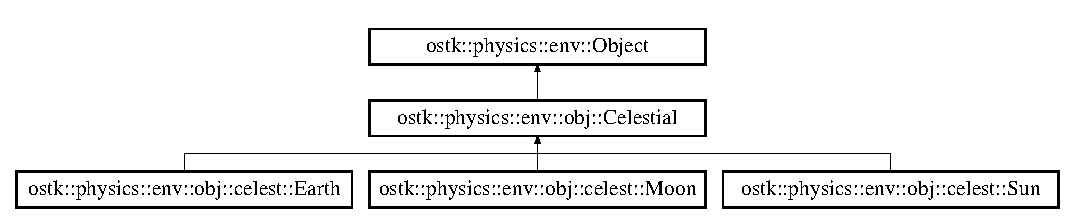
\includegraphics[height=2.568807cm]{classostk_1_1physics_1_1env_1_1obj_1_1_celestial}
\end{center}
\end{figure}
\subsection*{Classes}
\begin{DoxyCompactItemize}
\item 
struct \hyperlink{structostk_1_1physics_1_1env_1_1obj_1_1_celestial_1_1_model_base}{Model\+Base}
\end{DoxyCompactItemize}
\subsection*{Public Types}
\begin{DoxyCompactItemize}
\item 
enum \hyperlink{classostk_1_1physics_1_1env_1_1obj_1_1_celestial_aa0711d887522b35b2b3630156d912779}{Type} \{ \newline
\hyperlink{classostk_1_1physics_1_1env_1_1obj_1_1_celestial_aa0711d887522b35b2b3630156d912779aec0fc0100c4fc1ce4eea230c3dc10360}{Type\+::\+Undefined}, 
\hyperlink{classostk_1_1physics_1_1env_1_1obj_1_1_celestial_aa0711d887522b35b2b3630156d912779aef6572e4cd58bb39a3f4e82fc64fe9f0}{Type\+::\+Sun}, 
\hyperlink{classostk_1_1physics_1_1env_1_1obj_1_1_celestial_aa0711d887522b35b2b3630156d912779a34dae487e31f37aa74633258b7774d4f}{Type\+::\+Mercury}, 
\hyperlink{classostk_1_1physics_1_1env_1_1obj_1_1_celestial_aa0711d887522b35b2b3630156d912779a0bdc508a17811a3a860d32749ad44e4b}{Type\+::\+Venus}, 
\newline
\hyperlink{classostk_1_1physics_1_1env_1_1obj_1_1_celestial_aa0711d887522b35b2b3630156d912779a5cdd21c97f86686cc505e02fd32a7523}{Type\+::\+Earth}, 
\hyperlink{classostk_1_1physics_1_1env_1_1obj_1_1_celestial_aa0711d887522b35b2b3630156d912779ad502a50ed945d5fca74e0105575b5b34}{Type\+::\+Moon}, 
\hyperlink{classostk_1_1physics_1_1env_1_1obj_1_1_celestial_aa0711d887522b35b2b3630156d912779a671f028142280b556a85ffdd90e0a43d}{Type\+::\+Mars}
 \}
\item 
enum \hyperlink{classostk_1_1physics_1_1env_1_1obj_1_1_celestial_ad005258cdc5969759c8a516fb1cfd262}{Frame\+Type} \{ \hyperlink{classostk_1_1physics_1_1env_1_1obj_1_1_celestial_ad005258cdc5969759c8a516fb1cfd262aec0fc0100c4fc1ce4eea230c3dc10360}{Frame\+Type\+::\+Undefined}, 
\hyperlink{classostk_1_1physics_1_1env_1_1obj_1_1_celestial_ad005258cdc5969759c8a516fb1cfd262acd3459b28418fa8fa75ffaba4f3e7c74}{Frame\+Type\+::\+N\+ED}
 \}
\end{DoxyCompactItemize}
\subsection*{Public Member Functions}
\begin{DoxyCompactItemize}
\item 
\hyperlink{classostk_1_1physics_1_1env_1_1obj_1_1_celestial_a428093b00b3f96d733426a168b344984}{Celestial} (const String \&a\+Name, const \hyperlink{classostk_1_1physics_1_1env_1_1obj_1_1_celestial_aa0711d887522b35b2b3630156d912779}{Celestial\+::\+Type} \&a\+Type, const \hyperlink{classostk_1_1physics_1_1units_1_1_derived}{Derived} \&a\+Gravitational\+Parameter, const \hyperlink{classostk_1_1physics_1_1units_1_1_length}{Length} \&an\+Equatorial\+Radius, const Real \&a\+Flattening, const Real \&a\+J2, const Shared$<$ \hyperlink{classostk_1_1physics_1_1env_1_1_ephemeris}{Ephemeris} $>$ \&an\+Ephemeris, const Shared$<$ \hyperlink{namespaceostk_1_1physics_1_1env_1_1obj_a50c0bc72e8880f2fa2a910a81e050c97}{Gravitational\+Model} $>$ \&a\+Gravitational\+Model, const Shared$<$ \hyperlink{namespaceostk_1_1physics_1_1env_1_1obj_a11552c1290e2f6b4693ea00c2df2c80d}{Magnetic\+Model} $>$ \&a\+Magnetic\+Model, const \hyperlink{classostk_1_1physics_1_1time_1_1_instant}{Instant} \&an\+Instant)
\item 
\hyperlink{classostk_1_1physics_1_1env_1_1obj_1_1_celestial_a9519c2dacaeaf7b67fa7cae77eab427e}{Celestial} (const String \&a\+Name, const \hyperlink{classostk_1_1physics_1_1env_1_1obj_1_1_celestial_aa0711d887522b35b2b3630156d912779}{Celestial\+::\+Type} \&a\+Type, const \hyperlink{classostk_1_1physics_1_1units_1_1_derived}{Derived} \&a\+Gravitational\+Parameter, const \hyperlink{classostk_1_1physics_1_1units_1_1_length}{Length} \&an\+Equatorial\+Radius, const Real \&a\+Flattening, const Real \&a\+J2, const Shared$<$ \hyperlink{classostk_1_1physics_1_1env_1_1_ephemeris}{Ephemeris} $>$ \&an\+Ephemeris, const Shared$<$ \hyperlink{namespaceostk_1_1physics_1_1env_1_1obj_a50c0bc72e8880f2fa2a910a81e050c97}{Gravitational\+Model} $>$ \&a\+Gravitational\+Model, const Shared$<$ \hyperlink{namespaceostk_1_1physics_1_1env_1_1obj_a11552c1290e2f6b4693ea00c2df2c80d}{Magnetic\+Model} $>$ \&a\+Magnetic\+Model, const \hyperlink{classostk_1_1physics_1_1time_1_1_instant}{Instant} \&an\+Instant, const \hyperlink{classostk_1_1physics_1_1env_1_1_object_a66e44a65aefb23a184a6de531e96935d}{Object\+::\+Geometry} \&a\+Geometry)
\item 
virtual \hyperlink{classostk_1_1physics_1_1env_1_1obj_1_1_celestial_aadbeb101aaa4c4acb136278385d2080b}{$\sim$\+Celestial} () override
\item 
virtual \hyperlink{classostk_1_1physics_1_1env_1_1obj_1_1_celestial}{Celestial} $\ast$ \hyperlink{classostk_1_1physics_1_1env_1_1obj_1_1_celestial_a87c6f3ec3c0ec9758ae52e3edc3fc5df}{clone} () const override
\item 
virtual bool \hyperlink{classostk_1_1physics_1_1env_1_1obj_1_1_celestial_a611b8fe6fcd3787bbf9981ad99dfe471}{is\+Defined} () const override
\item 
Shared$<$ const \hyperlink{classostk_1_1physics_1_1env_1_1_ephemeris}{Ephemeris} $>$ \hyperlink{classostk_1_1physics_1_1env_1_1obj_1_1_celestial_a381edd898ce5b55e533a250a8212cf1b}{access\+Ephemeris} () const
\item 
Shared$<$ const \hyperlink{namespaceostk_1_1physics_1_1env_1_1obj_a50c0bc72e8880f2fa2a910a81e050c97}{Gravitational\+Model} $>$ \hyperlink{classostk_1_1physics_1_1env_1_1obj_1_1_celestial_ad498343cdb085c4bb626442e69c583b0}{access\+Gravitational\+Model} () const
\item 
Shared$<$ const \hyperlink{namespaceostk_1_1physics_1_1env_1_1obj_a11552c1290e2f6b4693ea00c2df2c80d}{Magnetic\+Model} $>$ \hyperlink{classostk_1_1physics_1_1env_1_1obj_1_1_celestial_a3bf6a51759025bf14f1d766348548b22}{access\+Magnetic\+Model} () const
\item 
\hyperlink{classostk_1_1physics_1_1env_1_1obj_1_1_celestial_aa0711d887522b35b2b3630156d912779}{Celestial\+::\+Type} \hyperlink{classostk_1_1physics_1_1env_1_1obj_1_1_celestial_ad5b0fb87f14be14519ecddd37f134719}{get\+Type} () const
\item 
\hyperlink{classostk_1_1physics_1_1units_1_1_derived}{Derived} \hyperlink{classostk_1_1physics_1_1env_1_1obj_1_1_celestial_a433a6bf852e23db369fec77f02e90647}{get\+Gravitational\+Parameter} () const
\item 
\hyperlink{classostk_1_1physics_1_1units_1_1_length}{Length} \hyperlink{classostk_1_1physics_1_1env_1_1obj_1_1_celestial_ad0d484832d406c1e5b57cab731f839f3}{get\+Equatorial\+Radius} () const
\item 
Real \hyperlink{classostk_1_1physics_1_1env_1_1obj_1_1_celestial_ac57af98c82cfc344f24d1a91f45e99ff}{get\+Flattening} () const
\item 
Real \hyperlink{classostk_1_1physics_1_1env_1_1obj_1_1_celestial_ac7b892c6433c93f227d53f59285aac1d}{get\+J2} () const
\item 
virtual Shared$<$ const \hyperlink{classostk_1_1physics_1_1coord_1_1_frame}{Frame} $>$ \hyperlink{classostk_1_1physics_1_1env_1_1obj_1_1_celestial_a0140fc682a707ec2dc715828e532db79}{access\+Frame} () const override
\item 
virtual \hyperlink{classostk_1_1physics_1_1coord_1_1_position}{Position} \hyperlink{classostk_1_1physics_1_1env_1_1obj_1_1_celestial_af38fd0017fe14cfb6103684fcb1d3ee9}{get\+Position\+In} (const Shared$<$ const \hyperlink{classostk_1_1physics_1_1coord_1_1_frame}{Frame} $>$ \&a\+Frame\+S\+Ptr) const override
\item 
virtual \hyperlink{classostk_1_1physics_1_1coord_1_1_velocity}{Velocity} \hyperlink{classostk_1_1physics_1_1env_1_1obj_1_1_celestial_a748a113566d79c463e84bf62f05af83a}{get\+Velocity\+In} (const Shared$<$ const \hyperlink{classostk_1_1physics_1_1coord_1_1_frame}{Frame} $>$ \&a\+Frame\+S\+Ptr) const override
\item 
virtual \hyperlink{classostk_1_1physics_1_1coord_1_1_transform}{Transform} \hyperlink{classostk_1_1physics_1_1env_1_1obj_1_1_celestial_a8fa63af32cf8785ff6d3762d6f8dcd86}{get\+Transform\+To} (const Shared$<$ const \hyperlink{classostk_1_1physics_1_1coord_1_1_frame}{Frame} $>$ \&a\+Frame\+S\+Ptr) const override
\item 
virtual \hyperlink{classostk_1_1physics_1_1coord_1_1_axes}{Axes} \hyperlink{classostk_1_1physics_1_1env_1_1obj_1_1_celestial_a52b8cd88b947ca97f94981e5d3e10677}{get\+Axes\+In} (const Shared$<$ const \hyperlink{classostk_1_1physics_1_1coord_1_1_frame}{Frame} $>$ \&a\+Frame\+S\+Ptr) const override
\item 
\hyperlink{classostk_1_1physics_1_1data_1_1_vector}{Vector} \hyperlink{classostk_1_1physics_1_1env_1_1obj_1_1_celestial_adc8df9d860d30eb49600e644f63045bc}{get\+Gravitational\+Field\+At} (const \hyperlink{classostk_1_1physics_1_1coord_1_1_position}{Position} \&a\+Position) const
\item 
\hyperlink{classostk_1_1physics_1_1data_1_1_vector}{Vector} \hyperlink{classostk_1_1physics_1_1env_1_1obj_1_1_celestial_ae2cd7ac1cb6a896390394b77cffa0297}{get\+Magnetic\+Field\+At} (const \hyperlink{classostk_1_1physics_1_1coord_1_1_position}{Position} \&a\+Position) const
\item 
Shared$<$ const \hyperlink{classostk_1_1physics_1_1coord_1_1_frame}{Frame} $>$ \hyperlink{classostk_1_1physics_1_1env_1_1obj_1_1_celestial_a6cd5d134347840891174cff0729e53b9}{get\+Frame\+At} (const \hyperlink{classostk_1_1physics_1_1coord_1_1spherical_1_1_l_l_a}{L\+LA} \&a\+Lla, const \hyperlink{classostk_1_1physics_1_1env_1_1obj_1_1_celestial_ad005258cdc5969759c8a516fb1cfd262}{Celestial\+::\+Frame\+Type} \&a\+Frame\+Type) const
\item 
\hyperlink{classostk_1_1physics_1_1env_1_1_object_a66e44a65aefb23a184a6de531e96935d}{Object\+::\+Geometry} \hyperlink{classostk_1_1physics_1_1env_1_1obj_1_1_celestial_a4c594d934cf5c6a25795d6a992ea564f}{get\+Terminator\+Geometry} () const
\end{DoxyCompactItemize}
\subsection*{Static Public Member Functions}
\begin{DoxyCompactItemize}
\item 
static \hyperlink{classostk_1_1physics_1_1env_1_1obj_1_1_celestial}{Celestial} \hyperlink{classostk_1_1physics_1_1env_1_1obj_1_1_celestial_ac27c062b04fa867e79c635dfd21808ca}{Undefined} ()
\item 
static String \hyperlink{classostk_1_1physics_1_1env_1_1obj_1_1_celestial_a6002c77288a58a9c523c667036a23164}{String\+From\+Frame\+Type} (const \hyperlink{classostk_1_1physics_1_1env_1_1obj_1_1_celestial_ad005258cdc5969759c8a516fb1cfd262}{Celestial\+::\+Frame\+Type} \&a\+Frame\+Type)
\end{DoxyCompactItemize}


\subsection{Member Enumeration Documentation}
\mbox{\Hypertarget{classostk_1_1physics_1_1env_1_1obj_1_1_celestial_ad005258cdc5969759c8a516fb1cfd262}\label{classostk_1_1physics_1_1env_1_1obj_1_1_celestial_ad005258cdc5969759c8a516fb1cfd262}} 
\index{ostk\+::physics\+::env\+::obj\+::\+Celestial@{ostk\+::physics\+::env\+::obj\+::\+Celestial}!Frame\+Type@{Frame\+Type}}
\index{Frame\+Type@{Frame\+Type}!ostk\+::physics\+::env\+::obj\+::\+Celestial@{ostk\+::physics\+::env\+::obj\+::\+Celestial}}
\subsubsection{\texorpdfstring{Frame\+Type}{FrameType}}
{\footnotesize\ttfamily enum \hyperlink{classostk_1_1physics_1_1env_1_1obj_1_1_celestial_ad005258cdc5969759c8a516fb1cfd262}{ostk\+::physics\+::env\+::obj\+::\+Celestial\+::\+Frame\+Type}\hspace{0.3cm}{\ttfamily [strong]}}

\begin{DoxyEnumFields}{Enumerator}
\raisebox{\heightof{T}}[0pt][0pt]{\index{Undefined@{Undefined}!ostk\+::physics\+::env\+::obj\+::\+Celestial@{ostk\+::physics\+::env\+::obj\+::\+Celestial}}\index{ostk\+::physics\+::env\+::obj\+::\+Celestial@{ostk\+::physics\+::env\+::obj\+::\+Celestial}!Undefined@{Undefined}}}\mbox{\Hypertarget{classostk_1_1physics_1_1env_1_1obj_1_1_celestial_ad005258cdc5969759c8a516fb1cfd262aec0fc0100c4fc1ce4eea230c3dc10360}\label{classostk_1_1physics_1_1env_1_1obj_1_1_celestial_ad005258cdc5969759c8a516fb1cfd262aec0fc0100c4fc1ce4eea230c3dc10360}} 
Undefined&Undefined frame. \\
\hline

\raisebox{\heightof{T}}[0pt][0pt]{\index{N\+ED@{N\+ED}!ostk\+::physics\+::env\+::obj\+::\+Celestial@{ostk\+::physics\+::env\+::obj\+::\+Celestial}}\index{ostk\+::physics\+::env\+::obj\+::\+Celestial@{ostk\+::physics\+::env\+::obj\+::\+Celestial}!N\+ED@{N\+ED}}}\mbox{\Hypertarget{classostk_1_1physics_1_1env_1_1obj_1_1_celestial_ad005258cdc5969759c8a516fb1cfd262acd3459b28418fa8fa75ffaba4f3e7c74}\label{classostk_1_1physics_1_1env_1_1obj_1_1_celestial_ad005258cdc5969759c8a516fb1cfd262acd3459b28418fa8fa75ffaba4f3e7c74}} 
N\+ED&North-\/\+East-\/\+Down (N\+ED) frame. \\
\hline

\end{DoxyEnumFields}
\mbox{\Hypertarget{classostk_1_1physics_1_1env_1_1obj_1_1_celestial_aa0711d887522b35b2b3630156d912779}\label{classostk_1_1physics_1_1env_1_1obj_1_1_celestial_aa0711d887522b35b2b3630156d912779}} 
\index{ostk\+::physics\+::env\+::obj\+::\+Celestial@{ostk\+::physics\+::env\+::obj\+::\+Celestial}!Type@{Type}}
\index{Type@{Type}!ostk\+::physics\+::env\+::obj\+::\+Celestial@{ostk\+::physics\+::env\+::obj\+::\+Celestial}}
\subsubsection{\texorpdfstring{Type}{Type}}
{\footnotesize\ttfamily enum \hyperlink{classostk_1_1physics_1_1env_1_1obj_1_1_celestial_aa0711d887522b35b2b3630156d912779}{ostk\+::physics\+::env\+::obj\+::\+Celestial\+::\+Type}\hspace{0.3cm}{\ttfamily [strong]}}

\begin{DoxyEnumFields}{Enumerator}
\raisebox{\heightof{T}}[0pt][0pt]{\index{Undefined@{Undefined}!ostk\+::physics\+::env\+::obj\+::\+Celestial@{ostk\+::physics\+::env\+::obj\+::\+Celestial}}\index{ostk\+::physics\+::env\+::obj\+::\+Celestial@{ostk\+::physics\+::env\+::obj\+::\+Celestial}!Undefined@{Undefined}}}\mbox{\Hypertarget{classostk_1_1physics_1_1env_1_1obj_1_1_celestial_aa0711d887522b35b2b3630156d912779aec0fc0100c4fc1ce4eea230c3dc10360}\label{classostk_1_1physics_1_1env_1_1obj_1_1_celestial_aa0711d887522b35b2b3630156d912779aec0fc0100c4fc1ce4eea230c3dc10360}} 
Undefined&\\
\hline

\raisebox{\heightof{T}}[0pt][0pt]{\index{Sun@{Sun}!ostk\+::physics\+::env\+::obj\+::\+Celestial@{ostk\+::physics\+::env\+::obj\+::\+Celestial}}\index{ostk\+::physics\+::env\+::obj\+::\+Celestial@{ostk\+::physics\+::env\+::obj\+::\+Celestial}!Sun@{Sun}}}\mbox{\Hypertarget{classostk_1_1physics_1_1env_1_1obj_1_1_celestial_aa0711d887522b35b2b3630156d912779aef6572e4cd58bb39a3f4e82fc64fe9f0}\label{classostk_1_1physics_1_1env_1_1obj_1_1_celestial_aa0711d887522b35b2b3630156d912779aef6572e4cd58bb39a3f4e82fc64fe9f0}} 
Sun&\\
\hline

\raisebox{\heightof{T}}[0pt][0pt]{\index{Mercury@{Mercury}!ostk\+::physics\+::env\+::obj\+::\+Celestial@{ostk\+::physics\+::env\+::obj\+::\+Celestial}}\index{ostk\+::physics\+::env\+::obj\+::\+Celestial@{ostk\+::physics\+::env\+::obj\+::\+Celestial}!Mercury@{Mercury}}}\mbox{\Hypertarget{classostk_1_1physics_1_1env_1_1obj_1_1_celestial_aa0711d887522b35b2b3630156d912779a34dae487e31f37aa74633258b7774d4f}\label{classostk_1_1physics_1_1env_1_1obj_1_1_celestial_aa0711d887522b35b2b3630156d912779a34dae487e31f37aa74633258b7774d4f}} 
Mercury&\\
\hline

\raisebox{\heightof{T}}[0pt][0pt]{\index{Venus@{Venus}!ostk\+::physics\+::env\+::obj\+::\+Celestial@{ostk\+::physics\+::env\+::obj\+::\+Celestial}}\index{ostk\+::physics\+::env\+::obj\+::\+Celestial@{ostk\+::physics\+::env\+::obj\+::\+Celestial}!Venus@{Venus}}}\mbox{\Hypertarget{classostk_1_1physics_1_1env_1_1obj_1_1_celestial_aa0711d887522b35b2b3630156d912779a0bdc508a17811a3a860d32749ad44e4b}\label{classostk_1_1physics_1_1env_1_1obj_1_1_celestial_aa0711d887522b35b2b3630156d912779a0bdc508a17811a3a860d32749ad44e4b}} 
Venus&\\
\hline

\raisebox{\heightof{T}}[0pt][0pt]{\index{Earth@{Earth}!ostk\+::physics\+::env\+::obj\+::\+Celestial@{ostk\+::physics\+::env\+::obj\+::\+Celestial}}\index{ostk\+::physics\+::env\+::obj\+::\+Celestial@{ostk\+::physics\+::env\+::obj\+::\+Celestial}!Earth@{Earth}}}\mbox{\Hypertarget{classostk_1_1physics_1_1env_1_1obj_1_1_celestial_aa0711d887522b35b2b3630156d912779a5cdd21c97f86686cc505e02fd32a7523}\label{classostk_1_1physics_1_1env_1_1obj_1_1_celestial_aa0711d887522b35b2b3630156d912779a5cdd21c97f86686cc505e02fd32a7523}} 
Earth&\\
\hline

\raisebox{\heightof{T}}[0pt][0pt]{\index{Moon@{Moon}!ostk\+::physics\+::env\+::obj\+::\+Celestial@{ostk\+::physics\+::env\+::obj\+::\+Celestial}}\index{ostk\+::physics\+::env\+::obj\+::\+Celestial@{ostk\+::physics\+::env\+::obj\+::\+Celestial}!Moon@{Moon}}}\mbox{\Hypertarget{classostk_1_1physics_1_1env_1_1obj_1_1_celestial_aa0711d887522b35b2b3630156d912779ad502a50ed945d5fca74e0105575b5b34}\label{classostk_1_1physics_1_1env_1_1obj_1_1_celestial_aa0711d887522b35b2b3630156d912779ad502a50ed945d5fca74e0105575b5b34}} 
Moon&\\
\hline

\raisebox{\heightof{T}}[0pt][0pt]{\index{Mars@{Mars}!ostk\+::physics\+::env\+::obj\+::\+Celestial@{ostk\+::physics\+::env\+::obj\+::\+Celestial}}\index{ostk\+::physics\+::env\+::obj\+::\+Celestial@{ostk\+::physics\+::env\+::obj\+::\+Celestial}!Mars@{Mars}}}\mbox{\Hypertarget{classostk_1_1physics_1_1env_1_1obj_1_1_celestial_aa0711d887522b35b2b3630156d912779a671f028142280b556a85ffdd90e0a43d}\label{classostk_1_1physics_1_1env_1_1obj_1_1_celestial_aa0711d887522b35b2b3630156d912779a671f028142280b556a85ffdd90e0a43d}} 
Mars&\\
\hline

\end{DoxyEnumFields}


\subsection{Constructor \& Destructor Documentation}
\mbox{\Hypertarget{classostk_1_1physics_1_1env_1_1obj_1_1_celestial_a428093b00b3f96d733426a168b344984}\label{classostk_1_1physics_1_1env_1_1obj_1_1_celestial_a428093b00b3f96d733426a168b344984}} 
\index{ostk\+::physics\+::env\+::obj\+::\+Celestial@{ostk\+::physics\+::env\+::obj\+::\+Celestial}!Celestial@{Celestial}}
\index{Celestial@{Celestial}!ostk\+::physics\+::env\+::obj\+::\+Celestial@{ostk\+::physics\+::env\+::obj\+::\+Celestial}}
\subsubsection{\texorpdfstring{Celestial()}{Celestial()}\hspace{0.1cm}{\footnotesize\ttfamily [1/2]}}
{\footnotesize\ttfamily ostk\+::physics\+::env\+::obj\+::\+Celestial\+::\+Celestial (\begin{DoxyParamCaption}\item[{const String \&}]{a\+Name,  }\item[{const \hyperlink{classostk_1_1physics_1_1env_1_1obj_1_1_celestial_aa0711d887522b35b2b3630156d912779}{Celestial\+::\+Type} \&}]{a\+Type,  }\item[{const \hyperlink{classostk_1_1physics_1_1units_1_1_derived}{Derived} \&}]{a\+Gravitational\+Parameter,  }\item[{const \hyperlink{classostk_1_1physics_1_1units_1_1_length}{Length} \&}]{an\+Equatorial\+Radius,  }\item[{const Real \&}]{a\+Flattening,  }\item[{const Real \&}]{a\+J2,  }\item[{const Shared$<$ \hyperlink{classostk_1_1physics_1_1env_1_1_ephemeris}{Ephemeris} $>$ \&}]{an\+Ephemeris,  }\item[{const Shared$<$ \hyperlink{namespaceostk_1_1physics_1_1env_1_1obj_a50c0bc72e8880f2fa2a910a81e050c97}{Gravitational\+Model} $>$ \&}]{a\+Gravitational\+Model,  }\item[{const Shared$<$ \hyperlink{namespaceostk_1_1physics_1_1env_1_1obj_a11552c1290e2f6b4693ea00c2df2c80d}{Magnetic\+Model} $>$ \&}]{a\+Magnetic\+Model,  }\item[{const \hyperlink{classostk_1_1physics_1_1time_1_1_instant}{Instant} \&}]{an\+Instant }\end{DoxyParamCaption})}

\mbox{\Hypertarget{classostk_1_1physics_1_1env_1_1obj_1_1_celestial_a9519c2dacaeaf7b67fa7cae77eab427e}\label{classostk_1_1physics_1_1env_1_1obj_1_1_celestial_a9519c2dacaeaf7b67fa7cae77eab427e}} 
\index{ostk\+::physics\+::env\+::obj\+::\+Celestial@{ostk\+::physics\+::env\+::obj\+::\+Celestial}!Celestial@{Celestial}}
\index{Celestial@{Celestial}!ostk\+::physics\+::env\+::obj\+::\+Celestial@{ostk\+::physics\+::env\+::obj\+::\+Celestial}}
\subsubsection{\texorpdfstring{Celestial()}{Celestial()}\hspace{0.1cm}{\footnotesize\ttfamily [2/2]}}
{\footnotesize\ttfamily ostk\+::physics\+::env\+::obj\+::\+Celestial\+::\+Celestial (\begin{DoxyParamCaption}\item[{const String \&}]{a\+Name,  }\item[{const \hyperlink{classostk_1_1physics_1_1env_1_1obj_1_1_celestial_aa0711d887522b35b2b3630156d912779}{Celestial\+::\+Type} \&}]{a\+Type,  }\item[{const \hyperlink{classostk_1_1physics_1_1units_1_1_derived}{Derived} \&}]{a\+Gravitational\+Parameter,  }\item[{const \hyperlink{classostk_1_1physics_1_1units_1_1_length}{Length} \&}]{an\+Equatorial\+Radius,  }\item[{const Real \&}]{a\+Flattening,  }\item[{const Real \&}]{a\+J2,  }\item[{const Shared$<$ \hyperlink{classostk_1_1physics_1_1env_1_1_ephemeris}{Ephemeris} $>$ \&}]{an\+Ephemeris,  }\item[{const Shared$<$ \hyperlink{namespaceostk_1_1physics_1_1env_1_1obj_a50c0bc72e8880f2fa2a910a81e050c97}{Gravitational\+Model} $>$ \&}]{a\+Gravitational\+Model,  }\item[{const Shared$<$ \hyperlink{namespaceostk_1_1physics_1_1env_1_1obj_a11552c1290e2f6b4693ea00c2df2c80d}{Magnetic\+Model} $>$ \&}]{a\+Magnetic\+Model,  }\item[{const \hyperlink{classostk_1_1physics_1_1time_1_1_instant}{Instant} \&}]{an\+Instant,  }\item[{const \hyperlink{classostk_1_1physics_1_1env_1_1_object_a66e44a65aefb23a184a6de531e96935d}{Object\+::\+Geometry} \&}]{a\+Geometry }\end{DoxyParamCaption})}

\mbox{\Hypertarget{classostk_1_1physics_1_1env_1_1obj_1_1_celestial_aadbeb101aaa4c4acb136278385d2080b}\label{classostk_1_1physics_1_1env_1_1obj_1_1_celestial_aadbeb101aaa4c4acb136278385d2080b}} 
\index{ostk\+::physics\+::env\+::obj\+::\+Celestial@{ostk\+::physics\+::env\+::obj\+::\+Celestial}!````~Celestial@{$\sim$\+Celestial}}
\index{````~Celestial@{$\sim$\+Celestial}!ostk\+::physics\+::env\+::obj\+::\+Celestial@{ostk\+::physics\+::env\+::obj\+::\+Celestial}}
\subsubsection{\texorpdfstring{$\sim$\+Celestial()}{~Celestial()}}
{\footnotesize\ttfamily ostk\+::physics\+::env\+::obj\+::\+Celestial\+::$\sim$\+Celestial (\begin{DoxyParamCaption}{ }\end{DoxyParamCaption})\hspace{0.3cm}{\ttfamily [override]}, {\ttfamily [virtual]}}



\subsection{Member Function Documentation}
\mbox{\Hypertarget{classostk_1_1physics_1_1env_1_1obj_1_1_celestial_a381edd898ce5b55e533a250a8212cf1b}\label{classostk_1_1physics_1_1env_1_1obj_1_1_celestial_a381edd898ce5b55e533a250a8212cf1b}} 
\index{ostk\+::physics\+::env\+::obj\+::\+Celestial@{ostk\+::physics\+::env\+::obj\+::\+Celestial}!access\+Ephemeris@{access\+Ephemeris}}
\index{access\+Ephemeris@{access\+Ephemeris}!ostk\+::physics\+::env\+::obj\+::\+Celestial@{ostk\+::physics\+::env\+::obj\+::\+Celestial}}
\subsubsection{\texorpdfstring{access\+Ephemeris()}{accessEphemeris()}}
{\footnotesize\ttfamily Shared$<$ const \hyperlink{classostk_1_1physics_1_1env_1_1_ephemeris}{Ephemeris} $>$ ostk\+::physics\+::env\+::obj\+::\+Celestial\+::access\+Ephemeris (\begin{DoxyParamCaption}{ }\end{DoxyParamCaption}) const}

\mbox{\Hypertarget{classostk_1_1physics_1_1env_1_1obj_1_1_celestial_a0140fc682a707ec2dc715828e532db79}\label{classostk_1_1physics_1_1env_1_1obj_1_1_celestial_a0140fc682a707ec2dc715828e532db79}} 
\index{ostk\+::physics\+::env\+::obj\+::\+Celestial@{ostk\+::physics\+::env\+::obj\+::\+Celestial}!access\+Frame@{access\+Frame}}
\index{access\+Frame@{access\+Frame}!ostk\+::physics\+::env\+::obj\+::\+Celestial@{ostk\+::physics\+::env\+::obj\+::\+Celestial}}
\subsubsection{\texorpdfstring{access\+Frame()}{accessFrame()}}
{\footnotesize\ttfamily Shared$<$ const \hyperlink{classostk_1_1physics_1_1coord_1_1_frame}{Frame} $>$ ostk\+::physics\+::env\+::obj\+::\+Celestial\+::access\+Frame (\begin{DoxyParamCaption}{ }\end{DoxyParamCaption}) const\hspace{0.3cm}{\ttfamily [override]}, {\ttfamily [virtual]}}



Implements \hyperlink{classostk_1_1physics_1_1env_1_1_object_aca93358323c3eb3e4dabf07c33187f14}{ostk\+::physics\+::env\+::\+Object}.

\mbox{\Hypertarget{classostk_1_1physics_1_1env_1_1obj_1_1_celestial_ad498343cdb085c4bb626442e69c583b0}\label{classostk_1_1physics_1_1env_1_1obj_1_1_celestial_ad498343cdb085c4bb626442e69c583b0}} 
\index{ostk\+::physics\+::env\+::obj\+::\+Celestial@{ostk\+::physics\+::env\+::obj\+::\+Celestial}!access\+Gravitational\+Model@{access\+Gravitational\+Model}}
\index{access\+Gravitational\+Model@{access\+Gravitational\+Model}!ostk\+::physics\+::env\+::obj\+::\+Celestial@{ostk\+::physics\+::env\+::obj\+::\+Celestial}}
\subsubsection{\texorpdfstring{access\+Gravitational\+Model()}{accessGravitationalModel()}}
{\footnotesize\ttfamily Shared$<$ const \hyperlink{namespaceostk_1_1physics_1_1env_1_1obj_a50c0bc72e8880f2fa2a910a81e050c97}{Gravitational\+Model} $>$ ostk\+::physics\+::env\+::obj\+::\+Celestial\+::access\+Gravitational\+Model (\begin{DoxyParamCaption}{ }\end{DoxyParamCaption}) const}

\mbox{\Hypertarget{classostk_1_1physics_1_1env_1_1obj_1_1_celestial_a3bf6a51759025bf14f1d766348548b22}\label{classostk_1_1physics_1_1env_1_1obj_1_1_celestial_a3bf6a51759025bf14f1d766348548b22}} 
\index{ostk\+::physics\+::env\+::obj\+::\+Celestial@{ostk\+::physics\+::env\+::obj\+::\+Celestial}!access\+Magnetic\+Model@{access\+Magnetic\+Model}}
\index{access\+Magnetic\+Model@{access\+Magnetic\+Model}!ostk\+::physics\+::env\+::obj\+::\+Celestial@{ostk\+::physics\+::env\+::obj\+::\+Celestial}}
\subsubsection{\texorpdfstring{access\+Magnetic\+Model()}{accessMagneticModel()}}
{\footnotesize\ttfamily Shared$<$ const \hyperlink{namespaceostk_1_1physics_1_1env_1_1obj_a11552c1290e2f6b4693ea00c2df2c80d}{Magnetic\+Model} $>$ ostk\+::physics\+::env\+::obj\+::\+Celestial\+::access\+Magnetic\+Model (\begin{DoxyParamCaption}{ }\end{DoxyParamCaption}) const}

\mbox{\Hypertarget{classostk_1_1physics_1_1env_1_1obj_1_1_celestial_a87c6f3ec3c0ec9758ae52e3edc3fc5df}\label{classostk_1_1physics_1_1env_1_1obj_1_1_celestial_a87c6f3ec3c0ec9758ae52e3edc3fc5df}} 
\index{ostk\+::physics\+::env\+::obj\+::\+Celestial@{ostk\+::physics\+::env\+::obj\+::\+Celestial}!clone@{clone}}
\index{clone@{clone}!ostk\+::physics\+::env\+::obj\+::\+Celestial@{ostk\+::physics\+::env\+::obj\+::\+Celestial}}
\subsubsection{\texorpdfstring{clone()}{clone()}}
{\footnotesize\ttfamily \hyperlink{classostk_1_1physics_1_1env_1_1obj_1_1_celestial}{Celestial} $\ast$ ostk\+::physics\+::env\+::obj\+::\+Celestial\+::clone (\begin{DoxyParamCaption}{ }\end{DoxyParamCaption}) const\hspace{0.3cm}{\ttfamily [override]}, {\ttfamily [virtual]}}



Implements \hyperlink{classostk_1_1physics_1_1env_1_1_object_a8e45ece3cf6d7be05a984a8857b7ecd3}{ostk\+::physics\+::env\+::\+Object}.



Reimplemented in \hyperlink{classostk_1_1physics_1_1env_1_1obj_1_1celest_1_1_earth_ae86664b9d6fc870baa1dac5c3219f784}{ostk\+::physics\+::env\+::obj\+::celest\+::\+Earth}, \hyperlink{classostk_1_1physics_1_1env_1_1obj_1_1celest_1_1_moon_adcfeda7b73d32df67f5b38c05ca9351a}{ostk\+::physics\+::env\+::obj\+::celest\+::\+Moon}, and \hyperlink{classostk_1_1physics_1_1env_1_1obj_1_1celest_1_1_sun_a57fd7c3c48115f77e2d3d331ef0e8e0a}{ostk\+::physics\+::env\+::obj\+::celest\+::\+Sun}.

\mbox{\Hypertarget{classostk_1_1physics_1_1env_1_1obj_1_1_celestial_a52b8cd88b947ca97f94981e5d3e10677}\label{classostk_1_1physics_1_1env_1_1obj_1_1_celestial_a52b8cd88b947ca97f94981e5d3e10677}} 
\index{ostk\+::physics\+::env\+::obj\+::\+Celestial@{ostk\+::physics\+::env\+::obj\+::\+Celestial}!get\+Axes\+In@{get\+Axes\+In}}
\index{get\+Axes\+In@{get\+Axes\+In}!ostk\+::physics\+::env\+::obj\+::\+Celestial@{ostk\+::physics\+::env\+::obj\+::\+Celestial}}
\subsubsection{\texorpdfstring{get\+Axes\+In()}{getAxesIn()}}
{\footnotesize\ttfamily \hyperlink{classostk_1_1physics_1_1coord_1_1_axes}{Axes} ostk\+::physics\+::env\+::obj\+::\+Celestial\+::get\+Axes\+In (\begin{DoxyParamCaption}\item[{const Shared$<$ const \hyperlink{classostk_1_1physics_1_1coord_1_1_frame}{Frame} $>$ \&}]{a\+Frame\+S\+Ptr }\end{DoxyParamCaption}) const\hspace{0.3cm}{\ttfamily [override]}, {\ttfamily [virtual]}}



Implements \hyperlink{classostk_1_1physics_1_1env_1_1_object_a706d29c77ce311a3abcf2a6060515711}{ostk\+::physics\+::env\+::\+Object}.

\mbox{\Hypertarget{classostk_1_1physics_1_1env_1_1obj_1_1_celestial_ad0d484832d406c1e5b57cab731f839f3}\label{classostk_1_1physics_1_1env_1_1obj_1_1_celestial_ad0d484832d406c1e5b57cab731f839f3}} 
\index{ostk\+::physics\+::env\+::obj\+::\+Celestial@{ostk\+::physics\+::env\+::obj\+::\+Celestial}!get\+Equatorial\+Radius@{get\+Equatorial\+Radius}}
\index{get\+Equatorial\+Radius@{get\+Equatorial\+Radius}!ostk\+::physics\+::env\+::obj\+::\+Celestial@{ostk\+::physics\+::env\+::obj\+::\+Celestial}}
\subsubsection{\texorpdfstring{get\+Equatorial\+Radius()}{getEquatorialRadius()}}
{\footnotesize\ttfamily \hyperlink{classostk_1_1physics_1_1units_1_1_length}{Length} ostk\+::physics\+::env\+::obj\+::\+Celestial\+::get\+Equatorial\+Radius (\begin{DoxyParamCaption}{ }\end{DoxyParamCaption}) const}

\mbox{\Hypertarget{classostk_1_1physics_1_1env_1_1obj_1_1_celestial_ac57af98c82cfc344f24d1a91f45e99ff}\label{classostk_1_1physics_1_1env_1_1obj_1_1_celestial_ac57af98c82cfc344f24d1a91f45e99ff}} 
\index{ostk\+::physics\+::env\+::obj\+::\+Celestial@{ostk\+::physics\+::env\+::obj\+::\+Celestial}!get\+Flattening@{get\+Flattening}}
\index{get\+Flattening@{get\+Flattening}!ostk\+::physics\+::env\+::obj\+::\+Celestial@{ostk\+::physics\+::env\+::obj\+::\+Celestial}}
\subsubsection{\texorpdfstring{get\+Flattening()}{getFlattening()}}
{\footnotesize\ttfamily Real ostk\+::physics\+::env\+::obj\+::\+Celestial\+::get\+Flattening (\begin{DoxyParamCaption}{ }\end{DoxyParamCaption}) const}

\mbox{\Hypertarget{classostk_1_1physics_1_1env_1_1obj_1_1_celestial_a6cd5d134347840891174cff0729e53b9}\label{classostk_1_1physics_1_1env_1_1obj_1_1_celestial_a6cd5d134347840891174cff0729e53b9}} 
\index{ostk\+::physics\+::env\+::obj\+::\+Celestial@{ostk\+::physics\+::env\+::obj\+::\+Celestial}!get\+Frame\+At@{get\+Frame\+At}}
\index{get\+Frame\+At@{get\+Frame\+At}!ostk\+::physics\+::env\+::obj\+::\+Celestial@{ostk\+::physics\+::env\+::obj\+::\+Celestial}}
\subsubsection{\texorpdfstring{get\+Frame\+At()}{getFrameAt()}}
{\footnotesize\ttfamily Shared$<$ const \hyperlink{classostk_1_1physics_1_1coord_1_1_frame}{Frame} $>$ ostk\+::physics\+::env\+::obj\+::\+Celestial\+::get\+Frame\+At (\begin{DoxyParamCaption}\item[{const \hyperlink{classostk_1_1physics_1_1coord_1_1spherical_1_1_l_l_a}{L\+LA} \&}]{a\+Lla,  }\item[{const \hyperlink{classostk_1_1physics_1_1env_1_1obj_1_1_celestial_ad005258cdc5969759c8a516fb1cfd262}{Celestial\+::\+Frame\+Type} \&}]{a\+Frame\+Type }\end{DoxyParamCaption}) const}

\mbox{\Hypertarget{classostk_1_1physics_1_1env_1_1obj_1_1_celestial_adc8df9d860d30eb49600e644f63045bc}\label{classostk_1_1physics_1_1env_1_1obj_1_1_celestial_adc8df9d860d30eb49600e644f63045bc}} 
\index{ostk\+::physics\+::env\+::obj\+::\+Celestial@{ostk\+::physics\+::env\+::obj\+::\+Celestial}!get\+Gravitational\+Field\+At@{get\+Gravitational\+Field\+At}}
\index{get\+Gravitational\+Field\+At@{get\+Gravitational\+Field\+At}!ostk\+::physics\+::env\+::obj\+::\+Celestial@{ostk\+::physics\+::env\+::obj\+::\+Celestial}}
\subsubsection{\texorpdfstring{get\+Gravitational\+Field\+At()}{getGravitationalFieldAt()}}
{\footnotesize\ttfamily \hyperlink{classostk_1_1physics_1_1data_1_1_vector}{Vector} ostk\+::physics\+::env\+::obj\+::\+Celestial\+::get\+Gravitational\+Field\+At (\begin{DoxyParamCaption}\item[{const \hyperlink{classostk_1_1physics_1_1coord_1_1_position}{Position} \&}]{a\+Position }\end{DoxyParamCaption}) const}

\mbox{\Hypertarget{classostk_1_1physics_1_1env_1_1obj_1_1_celestial_a433a6bf852e23db369fec77f02e90647}\label{classostk_1_1physics_1_1env_1_1obj_1_1_celestial_a433a6bf852e23db369fec77f02e90647}} 
\index{ostk\+::physics\+::env\+::obj\+::\+Celestial@{ostk\+::physics\+::env\+::obj\+::\+Celestial}!get\+Gravitational\+Parameter@{get\+Gravitational\+Parameter}}
\index{get\+Gravitational\+Parameter@{get\+Gravitational\+Parameter}!ostk\+::physics\+::env\+::obj\+::\+Celestial@{ostk\+::physics\+::env\+::obj\+::\+Celestial}}
\subsubsection{\texorpdfstring{get\+Gravitational\+Parameter()}{getGravitationalParameter()}}
{\footnotesize\ttfamily \hyperlink{classostk_1_1physics_1_1units_1_1_derived}{Derived} ostk\+::physics\+::env\+::obj\+::\+Celestial\+::get\+Gravitational\+Parameter (\begin{DoxyParamCaption}{ }\end{DoxyParamCaption}) const}

\mbox{\Hypertarget{classostk_1_1physics_1_1env_1_1obj_1_1_celestial_ac7b892c6433c93f227d53f59285aac1d}\label{classostk_1_1physics_1_1env_1_1obj_1_1_celestial_ac7b892c6433c93f227d53f59285aac1d}} 
\index{ostk\+::physics\+::env\+::obj\+::\+Celestial@{ostk\+::physics\+::env\+::obj\+::\+Celestial}!get\+J2@{get\+J2}}
\index{get\+J2@{get\+J2}!ostk\+::physics\+::env\+::obj\+::\+Celestial@{ostk\+::physics\+::env\+::obj\+::\+Celestial}}
\subsubsection{\texorpdfstring{get\+J2()}{getJ2()}}
{\footnotesize\ttfamily Real ostk\+::physics\+::env\+::obj\+::\+Celestial\+::get\+J2 (\begin{DoxyParamCaption}{ }\end{DoxyParamCaption}) const}

\mbox{\Hypertarget{classostk_1_1physics_1_1env_1_1obj_1_1_celestial_ae2cd7ac1cb6a896390394b77cffa0297}\label{classostk_1_1physics_1_1env_1_1obj_1_1_celestial_ae2cd7ac1cb6a896390394b77cffa0297}} 
\index{ostk\+::physics\+::env\+::obj\+::\+Celestial@{ostk\+::physics\+::env\+::obj\+::\+Celestial}!get\+Magnetic\+Field\+At@{get\+Magnetic\+Field\+At}}
\index{get\+Magnetic\+Field\+At@{get\+Magnetic\+Field\+At}!ostk\+::physics\+::env\+::obj\+::\+Celestial@{ostk\+::physics\+::env\+::obj\+::\+Celestial}}
\subsubsection{\texorpdfstring{get\+Magnetic\+Field\+At()}{getMagneticFieldAt()}}
{\footnotesize\ttfamily \hyperlink{classostk_1_1physics_1_1data_1_1_vector}{Vector} ostk\+::physics\+::env\+::obj\+::\+Celestial\+::get\+Magnetic\+Field\+At (\begin{DoxyParamCaption}\item[{const \hyperlink{classostk_1_1physics_1_1coord_1_1_position}{Position} \&}]{a\+Position }\end{DoxyParamCaption}) const}

\mbox{\Hypertarget{classostk_1_1physics_1_1env_1_1obj_1_1_celestial_af38fd0017fe14cfb6103684fcb1d3ee9}\label{classostk_1_1physics_1_1env_1_1obj_1_1_celestial_af38fd0017fe14cfb6103684fcb1d3ee9}} 
\index{ostk\+::physics\+::env\+::obj\+::\+Celestial@{ostk\+::physics\+::env\+::obj\+::\+Celestial}!get\+Position\+In@{get\+Position\+In}}
\index{get\+Position\+In@{get\+Position\+In}!ostk\+::physics\+::env\+::obj\+::\+Celestial@{ostk\+::physics\+::env\+::obj\+::\+Celestial}}
\subsubsection{\texorpdfstring{get\+Position\+In()}{getPositionIn()}}
{\footnotesize\ttfamily \hyperlink{classostk_1_1physics_1_1coord_1_1_position}{Position} ostk\+::physics\+::env\+::obj\+::\+Celestial\+::get\+Position\+In (\begin{DoxyParamCaption}\item[{const Shared$<$ const \hyperlink{classostk_1_1physics_1_1coord_1_1_frame}{Frame} $>$ \&}]{a\+Frame\+S\+Ptr }\end{DoxyParamCaption}) const\hspace{0.3cm}{\ttfamily [override]}, {\ttfamily [virtual]}}



Implements \hyperlink{classostk_1_1physics_1_1env_1_1_object_a990c33e0cc9e9421488f9fc4cbbf3f21}{ostk\+::physics\+::env\+::\+Object}.

\mbox{\Hypertarget{classostk_1_1physics_1_1env_1_1obj_1_1_celestial_a4c594d934cf5c6a25795d6a992ea564f}\label{classostk_1_1physics_1_1env_1_1obj_1_1_celestial_a4c594d934cf5c6a25795d6a992ea564f}} 
\index{ostk\+::physics\+::env\+::obj\+::\+Celestial@{ostk\+::physics\+::env\+::obj\+::\+Celestial}!get\+Terminator\+Geometry@{get\+Terminator\+Geometry}}
\index{get\+Terminator\+Geometry@{get\+Terminator\+Geometry}!ostk\+::physics\+::env\+::obj\+::\+Celestial@{ostk\+::physics\+::env\+::obj\+::\+Celestial}}
\subsubsection{\texorpdfstring{get\+Terminator\+Geometry()}{getTerminatorGeometry()}}
{\footnotesize\ttfamily \hyperlink{classostk_1_1physics_1_1env_1_1_object_a66e44a65aefb23a184a6de531e96935d}{Object\+::\+Geometry} ostk\+::physics\+::env\+::obj\+::\+Celestial\+::get\+Terminator\+Geometry (\begin{DoxyParamCaption}{ }\end{DoxyParamCaption}) const}

\mbox{\Hypertarget{classostk_1_1physics_1_1env_1_1obj_1_1_celestial_a8fa63af32cf8785ff6d3762d6f8dcd86}\label{classostk_1_1physics_1_1env_1_1obj_1_1_celestial_a8fa63af32cf8785ff6d3762d6f8dcd86}} 
\index{ostk\+::physics\+::env\+::obj\+::\+Celestial@{ostk\+::physics\+::env\+::obj\+::\+Celestial}!get\+Transform\+To@{get\+Transform\+To}}
\index{get\+Transform\+To@{get\+Transform\+To}!ostk\+::physics\+::env\+::obj\+::\+Celestial@{ostk\+::physics\+::env\+::obj\+::\+Celestial}}
\subsubsection{\texorpdfstring{get\+Transform\+To()}{getTransformTo()}}
{\footnotesize\ttfamily \hyperlink{classostk_1_1physics_1_1coord_1_1_transform}{Transform} ostk\+::physics\+::env\+::obj\+::\+Celestial\+::get\+Transform\+To (\begin{DoxyParamCaption}\item[{const Shared$<$ const \hyperlink{classostk_1_1physics_1_1coord_1_1_frame}{Frame} $>$ \&}]{a\+Frame\+S\+Ptr }\end{DoxyParamCaption}) const\hspace{0.3cm}{\ttfamily [override]}, {\ttfamily [virtual]}}



Implements \hyperlink{classostk_1_1physics_1_1env_1_1_object_a720f81e696c3f4f81de8e7ae787fdf10}{ostk\+::physics\+::env\+::\+Object}.

\mbox{\Hypertarget{classostk_1_1physics_1_1env_1_1obj_1_1_celestial_ad5b0fb87f14be14519ecddd37f134719}\label{classostk_1_1physics_1_1env_1_1obj_1_1_celestial_ad5b0fb87f14be14519ecddd37f134719}} 
\index{ostk\+::physics\+::env\+::obj\+::\+Celestial@{ostk\+::physics\+::env\+::obj\+::\+Celestial}!get\+Type@{get\+Type}}
\index{get\+Type@{get\+Type}!ostk\+::physics\+::env\+::obj\+::\+Celestial@{ostk\+::physics\+::env\+::obj\+::\+Celestial}}
\subsubsection{\texorpdfstring{get\+Type()}{getType()}}
{\footnotesize\ttfamily \hyperlink{classostk_1_1physics_1_1env_1_1obj_1_1_celestial_aa0711d887522b35b2b3630156d912779}{Celestial\+::\+Type} ostk\+::physics\+::env\+::obj\+::\+Celestial\+::get\+Type (\begin{DoxyParamCaption}{ }\end{DoxyParamCaption}) const}

\mbox{\Hypertarget{classostk_1_1physics_1_1env_1_1obj_1_1_celestial_a748a113566d79c463e84bf62f05af83a}\label{classostk_1_1physics_1_1env_1_1obj_1_1_celestial_a748a113566d79c463e84bf62f05af83a}} 
\index{ostk\+::physics\+::env\+::obj\+::\+Celestial@{ostk\+::physics\+::env\+::obj\+::\+Celestial}!get\+Velocity\+In@{get\+Velocity\+In}}
\index{get\+Velocity\+In@{get\+Velocity\+In}!ostk\+::physics\+::env\+::obj\+::\+Celestial@{ostk\+::physics\+::env\+::obj\+::\+Celestial}}
\subsubsection{\texorpdfstring{get\+Velocity\+In()}{getVelocityIn()}}
{\footnotesize\ttfamily \hyperlink{classostk_1_1physics_1_1coord_1_1_velocity}{Velocity} ostk\+::physics\+::env\+::obj\+::\+Celestial\+::get\+Velocity\+In (\begin{DoxyParamCaption}\item[{const Shared$<$ const \hyperlink{classostk_1_1physics_1_1coord_1_1_frame}{Frame} $>$ \&}]{a\+Frame\+S\+Ptr }\end{DoxyParamCaption}) const\hspace{0.3cm}{\ttfamily [override]}, {\ttfamily [virtual]}}



Implements \hyperlink{classostk_1_1physics_1_1env_1_1_object_a216c8d5e44451fd664e0c7eb3b4934b6}{ostk\+::physics\+::env\+::\+Object}.

\mbox{\Hypertarget{classostk_1_1physics_1_1env_1_1obj_1_1_celestial_a611b8fe6fcd3787bbf9981ad99dfe471}\label{classostk_1_1physics_1_1env_1_1obj_1_1_celestial_a611b8fe6fcd3787bbf9981ad99dfe471}} 
\index{ostk\+::physics\+::env\+::obj\+::\+Celestial@{ostk\+::physics\+::env\+::obj\+::\+Celestial}!is\+Defined@{is\+Defined}}
\index{is\+Defined@{is\+Defined}!ostk\+::physics\+::env\+::obj\+::\+Celestial@{ostk\+::physics\+::env\+::obj\+::\+Celestial}}
\subsubsection{\texorpdfstring{is\+Defined()}{isDefined()}}
{\footnotesize\ttfamily bool ostk\+::physics\+::env\+::obj\+::\+Celestial\+::is\+Defined (\begin{DoxyParamCaption}{ }\end{DoxyParamCaption}) const\hspace{0.3cm}{\ttfamily [override]}, {\ttfamily [virtual]}}



Reimplemented from \hyperlink{classostk_1_1physics_1_1env_1_1_object_aaa5131bafbaf86fde7f649e88343a901}{ostk\+::physics\+::env\+::\+Object}.

\mbox{\Hypertarget{classostk_1_1physics_1_1env_1_1obj_1_1_celestial_a6002c77288a58a9c523c667036a23164}\label{classostk_1_1physics_1_1env_1_1obj_1_1_celestial_a6002c77288a58a9c523c667036a23164}} 
\index{ostk\+::physics\+::env\+::obj\+::\+Celestial@{ostk\+::physics\+::env\+::obj\+::\+Celestial}!String\+From\+Frame\+Type@{String\+From\+Frame\+Type}}
\index{String\+From\+Frame\+Type@{String\+From\+Frame\+Type}!ostk\+::physics\+::env\+::obj\+::\+Celestial@{ostk\+::physics\+::env\+::obj\+::\+Celestial}}
\subsubsection{\texorpdfstring{String\+From\+Frame\+Type()}{StringFromFrameType()}}
{\footnotesize\ttfamily String ostk\+::physics\+::env\+::obj\+::\+Celestial\+::\+String\+From\+Frame\+Type (\begin{DoxyParamCaption}\item[{const \hyperlink{classostk_1_1physics_1_1env_1_1obj_1_1_celestial_ad005258cdc5969759c8a516fb1cfd262}{Celestial\+::\+Frame\+Type} \&}]{a\+Frame\+Type }\end{DoxyParamCaption})\hspace{0.3cm}{\ttfamily [static]}}

\mbox{\Hypertarget{classostk_1_1physics_1_1env_1_1obj_1_1_celestial_ac27c062b04fa867e79c635dfd21808ca}\label{classostk_1_1physics_1_1env_1_1obj_1_1_celestial_ac27c062b04fa867e79c635dfd21808ca}} 
\index{ostk\+::physics\+::env\+::obj\+::\+Celestial@{ostk\+::physics\+::env\+::obj\+::\+Celestial}!Undefined@{Undefined}}
\index{Undefined@{Undefined}!ostk\+::physics\+::env\+::obj\+::\+Celestial@{ostk\+::physics\+::env\+::obj\+::\+Celestial}}
\subsubsection{\texorpdfstring{Undefined()}{Undefined()}}
{\footnotesize\ttfamily \hyperlink{classostk_1_1physics_1_1env_1_1obj_1_1_celestial}{Celestial} ostk\+::physics\+::env\+::obj\+::\+Celestial\+::\+Undefined (\begin{DoxyParamCaption}{ }\end{DoxyParamCaption})\hspace{0.3cm}{\ttfamily [static]}}



The documentation for this class was generated from the following files\+:\begin{DoxyCompactItemize}
\item 
include/\+Open\+Space\+Toolkit/\+Physics/\+Environment/\+Objects/\hyperlink{_celestial_8hpp}{Celestial.\+hpp}\item 
src/\+Open\+Space\+Toolkit/\+Physics/\+Environment/\+Objects/\hyperlink{_celestial_8cpp}{Celestial.\+cpp}\end{DoxyCompactItemize}

\hypertarget{classostk_1_1physics_1_1coord_1_1frame_1_1provider_1_1_c_i_r_f}{}\section{ostk\+:\+:physics\+:\+:coord\+:\+:frame\+:\+:provider\+:\+:C\+I\+RF Class Reference}
\label{classostk_1_1physics_1_1coord_1_1frame_1_1provider_1_1_c_i_r_f}\index{ostk\+::physics\+::coord\+::frame\+::provider\+::\+C\+I\+RF@{ostk\+::physics\+::coord\+::frame\+::provider\+::\+C\+I\+RF}}


Celestial Intermediate Reference \hyperlink{classostk_1_1physics_1_1coord_1_1_frame}{Frame} (\hyperlink{classostk_1_1physics_1_1coord_1_1frame_1_1provider_1_1_c_i_r_f}{C\+I\+RF}) provider.  




{\ttfamily \#include $<$C\+I\+R\+F.\+hpp$>$}

Inheritance diagram for ostk\+:\+:physics\+:\+:coord\+:\+:frame\+:\+:provider\+:\+:C\+I\+RF\+:\begin{figure}[H]
\begin{center}
\leavevmode
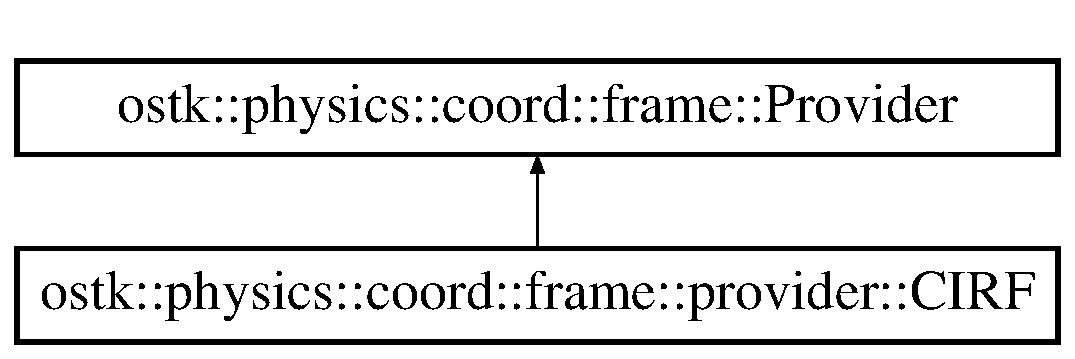
\includegraphics[height=2.000000cm]{classostk_1_1physics_1_1coord_1_1frame_1_1provider_1_1_c_i_r_f}
\end{center}
\end{figure}
\subsection*{Public Member Functions}
\begin{DoxyCompactItemize}
\item 
\hyperlink{classostk_1_1physics_1_1coord_1_1frame_1_1provider_1_1_c_i_r_f_ae7331c8b1396a6ba64833232eeded44d}{C\+I\+RF} ()
\item 
virtual \hyperlink{classostk_1_1physics_1_1coord_1_1frame_1_1provider_1_1_c_i_r_f_aba9f49808bea3b91c88a5d08f4330218}{$\sim$\+C\+I\+RF} () override
\item 
virtual \hyperlink{classostk_1_1physics_1_1coord_1_1frame_1_1provider_1_1_c_i_r_f}{C\+I\+RF} $\ast$ \hyperlink{classostk_1_1physics_1_1coord_1_1frame_1_1provider_1_1_c_i_r_f_a9c7c1e79785b676501e6a4686389a425}{clone} () const override
\item 
virtual bool \hyperlink{classostk_1_1physics_1_1coord_1_1frame_1_1provider_1_1_c_i_r_f_affec3924a864a0d793ee5aa887a06cf8}{is\+Defined} () const override
\item 
virtual \hyperlink{classostk_1_1physics_1_1coord_1_1_transform}{Transform} \hyperlink{classostk_1_1physics_1_1coord_1_1frame_1_1provider_1_1_c_i_r_f_a9a9cdbec164d2f54cfdaa2a1a62c3250}{get\+Transform\+At} (const \hyperlink{classostk_1_1physics_1_1time_1_1_instant}{Instant} \&an\+Instant) const override
\end{DoxyCompactItemize}


\subsection{Detailed Description}
Celestial Intermediate Reference \hyperlink{classostk_1_1physics_1_1coord_1_1_frame}{Frame} (\hyperlink{classostk_1_1physics_1_1coord_1_1frame_1_1provider_1_1_c_i_r_f}{C\+I\+RF}) provider. 

Bias, precession-\/nutation

https\+://www.iers.\+org/\+Shared\+Docs/\+Publikationen/\+E\+N/\+I\+E\+R\+S/\+Publications/tn/\+Techn\+Note36/tn36\+\_\+174.pdf?\+\_\+\+\_\+blob=publication\+File\&v=1 

\subsection{Constructor \& Destructor Documentation}
\mbox{\Hypertarget{classostk_1_1physics_1_1coord_1_1frame_1_1provider_1_1_c_i_r_f_ae7331c8b1396a6ba64833232eeded44d}\label{classostk_1_1physics_1_1coord_1_1frame_1_1provider_1_1_c_i_r_f_ae7331c8b1396a6ba64833232eeded44d}} 
\index{ostk\+::physics\+::coord\+::frame\+::provider\+::\+C\+I\+RF@{ostk\+::physics\+::coord\+::frame\+::provider\+::\+C\+I\+RF}!C\+I\+RF@{C\+I\+RF}}
\index{C\+I\+RF@{C\+I\+RF}!ostk\+::physics\+::coord\+::frame\+::provider\+::\+C\+I\+RF@{ostk\+::physics\+::coord\+::frame\+::provider\+::\+C\+I\+RF}}
\subsubsection{\texorpdfstring{C\+I\+R\+F()}{CIRF()}}
{\footnotesize\ttfamily ostk\+::physics\+::coord\+::frame\+::provider\+::\+C\+I\+R\+F\+::\+C\+I\+RF (\begin{DoxyParamCaption}{ }\end{DoxyParamCaption})}

\mbox{\Hypertarget{classostk_1_1physics_1_1coord_1_1frame_1_1provider_1_1_c_i_r_f_aba9f49808bea3b91c88a5d08f4330218}\label{classostk_1_1physics_1_1coord_1_1frame_1_1provider_1_1_c_i_r_f_aba9f49808bea3b91c88a5d08f4330218}} 
\index{ostk\+::physics\+::coord\+::frame\+::provider\+::\+C\+I\+RF@{ostk\+::physics\+::coord\+::frame\+::provider\+::\+C\+I\+RF}!````~C\+I\+RF@{$\sim$\+C\+I\+RF}}
\index{````~C\+I\+RF@{$\sim$\+C\+I\+RF}!ostk\+::physics\+::coord\+::frame\+::provider\+::\+C\+I\+RF@{ostk\+::physics\+::coord\+::frame\+::provider\+::\+C\+I\+RF}}
\subsubsection{\texorpdfstring{$\sim$\+C\+I\+R\+F()}{~CIRF()}}
{\footnotesize\ttfamily ostk\+::physics\+::coord\+::frame\+::provider\+::\+C\+I\+R\+F\+::$\sim$\+C\+I\+RF (\begin{DoxyParamCaption}{ }\end{DoxyParamCaption})\hspace{0.3cm}{\ttfamily [override]}, {\ttfamily [virtual]}}



\subsection{Member Function Documentation}
\mbox{\Hypertarget{classostk_1_1physics_1_1coord_1_1frame_1_1provider_1_1_c_i_r_f_a9c7c1e79785b676501e6a4686389a425}\label{classostk_1_1physics_1_1coord_1_1frame_1_1provider_1_1_c_i_r_f_a9c7c1e79785b676501e6a4686389a425}} 
\index{ostk\+::physics\+::coord\+::frame\+::provider\+::\+C\+I\+RF@{ostk\+::physics\+::coord\+::frame\+::provider\+::\+C\+I\+RF}!clone@{clone}}
\index{clone@{clone}!ostk\+::physics\+::coord\+::frame\+::provider\+::\+C\+I\+RF@{ostk\+::physics\+::coord\+::frame\+::provider\+::\+C\+I\+RF}}
\subsubsection{\texorpdfstring{clone()}{clone()}}
{\footnotesize\ttfamily \hyperlink{classostk_1_1physics_1_1coord_1_1frame_1_1provider_1_1_c_i_r_f}{C\+I\+RF} $\ast$ ostk\+::physics\+::coord\+::frame\+::provider\+::\+C\+I\+R\+F\+::clone (\begin{DoxyParamCaption}{ }\end{DoxyParamCaption}) const\hspace{0.3cm}{\ttfamily [override]}, {\ttfamily [virtual]}}



Implements \hyperlink{classostk_1_1physics_1_1coord_1_1frame_1_1_provider_ae41bc3862d088e9c8d90a79253294ce9}{ostk\+::physics\+::coord\+::frame\+::\+Provider}.

\mbox{\Hypertarget{classostk_1_1physics_1_1coord_1_1frame_1_1provider_1_1_c_i_r_f_a9a9cdbec164d2f54cfdaa2a1a62c3250}\label{classostk_1_1physics_1_1coord_1_1frame_1_1provider_1_1_c_i_r_f_a9a9cdbec164d2f54cfdaa2a1a62c3250}} 
\index{ostk\+::physics\+::coord\+::frame\+::provider\+::\+C\+I\+RF@{ostk\+::physics\+::coord\+::frame\+::provider\+::\+C\+I\+RF}!get\+Transform\+At@{get\+Transform\+At}}
\index{get\+Transform\+At@{get\+Transform\+At}!ostk\+::physics\+::coord\+::frame\+::provider\+::\+C\+I\+RF@{ostk\+::physics\+::coord\+::frame\+::provider\+::\+C\+I\+RF}}
\subsubsection{\texorpdfstring{get\+Transform\+At()}{getTransformAt()}}
{\footnotesize\ttfamily \hyperlink{classostk_1_1physics_1_1coord_1_1_transform}{Transform} ostk\+::physics\+::coord\+::frame\+::provider\+::\+C\+I\+R\+F\+::get\+Transform\+At (\begin{DoxyParamCaption}\item[{const \hyperlink{classostk_1_1physics_1_1time_1_1_instant}{Instant} \&}]{an\+Instant }\end{DoxyParamCaption}) const\hspace{0.3cm}{\ttfamily [override]}, {\ttfamily [virtual]}}



Implements \hyperlink{classostk_1_1physics_1_1coord_1_1frame_1_1_provider_a38b86a589f46f8b8a9c97ab2776f37d1}{ostk\+::physics\+::coord\+::frame\+::\+Provider}.

\mbox{\Hypertarget{classostk_1_1physics_1_1coord_1_1frame_1_1provider_1_1_c_i_r_f_affec3924a864a0d793ee5aa887a06cf8}\label{classostk_1_1physics_1_1coord_1_1frame_1_1provider_1_1_c_i_r_f_affec3924a864a0d793ee5aa887a06cf8}} 
\index{ostk\+::physics\+::coord\+::frame\+::provider\+::\+C\+I\+RF@{ostk\+::physics\+::coord\+::frame\+::provider\+::\+C\+I\+RF}!is\+Defined@{is\+Defined}}
\index{is\+Defined@{is\+Defined}!ostk\+::physics\+::coord\+::frame\+::provider\+::\+C\+I\+RF@{ostk\+::physics\+::coord\+::frame\+::provider\+::\+C\+I\+RF}}
\subsubsection{\texorpdfstring{is\+Defined()}{isDefined()}}
{\footnotesize\ttfamily bool ostk\+::physics\+::coord\+::frame\+::provider\+::\+C\+I\+R\+F\+::is\+Defined (\begin{DoxyParamCaption}{ }\end{DoxyParamCaption}) const\hspace{0.3cm}{\ttfamily [override]}, {\ttfamily [virtual]}}



Implements \hyperlink{classostk_1_1physics_1_1coord_1_1frame_1_1_provider_a27acab0012649796b97956fed1a91493}{ostk\+::physics\+::coord\+::frame\+::\+Provider}.



The documentation for this class was generated from the following files\+:\begin{DoxyCompactItemize}
\item 
include/\+Open\+Space\+Toolkit/\+Physics/\+Coordinate/\+Frame/\+Providers/\hyperlink{_c_i_r_f_8hpp}{C\+I\+R\+F.\+hpp}\item 
src/\+Open\+Space\+Toolkit/\+Physics/\+Coordinate/\+Frame/\+Providers/\hyperlink{_c_i_r_f_8cpp}{C\+I\+R\+F.\+cpp}\end{DoxyCompactItemize}

\hypertarget{structostk_1_1physics_1_1coord_1_1frame_1_1provider_1_1iers_1_1_finals2000_a_1_1_data}{}\section{ostk\+:\+:physics\+:\+:coord\+:\+:frame\+:\+:provider\+:\+:iers\+:\+:Finals2000A\+:\+:Data Struct Reference}
\label{structostk_1_1physics_1_1coord_1_1frame_1_1provider_1_1iers_1_1_finals2000_a_1_1_data}\index{ostk\+::physics\+::coord\+::frame\+::provider\+::iers\+::\+Finals2000\+A\+::\+Data@{ostk\+::physics\+::coord\+::frame\+::provider\+::iers\+::\+Finals2000\+A\+::\+Data}}


{\ttfamily \#include $<$Finals2000\+A.\+hpp$>$}

\subsection*{Public Attributes}
\begin{DoxyCompactItemize}
\item 
Integer \hyperlink{structostk_1_1physics_1_1coord_1_1frame_1_1provider_1_1iers_1_1_finals2000_a_1_1_data_aaa754f31dcd1fa19aeb7bd78cb14350b}{year}
\begin{DoxyCompactList}\small\item\em Year (to get true calendar year, add 1900 for M\+JD $<$= 51543 or add 2000 for M\+JD $>$= 51544) \end{DoxyCompactList}\item 
Integer \hyperlink{structostk_1_1physics_1_1coord_1_1frame_1_1provider_1_1iers_1_1_finals2000_a_1_1_data_a0f2aaef83fa75a1531e6457b24cc214e}{month}
\begin{DoxyCompactList}\small\item\em Month number. \end{DoxyCompactList}\item 
Integer \hyperlink{structostk_1_1physics_1_1coord_1_1frame_1_1provider_1_1iers_1_1_finals2000_a_1_1_data_a13410abac810082e6ba0baf1d12bb68f}{day}
\begin{DoxyCompactList}\small\item\em Day of month. \end{DoxyCompactList}\item 
Real \hyperlink{structostk_1_1physics_1_1coord_1_1frame_1_1provider_1_1iers_1_1_finals2000_a_1_1_data_a70f37f98aee1bebe57bcc12fae786bda}{mjd}
\begin{DoxyCompactList}\small\item\em Fractional Modified Julian Date (M\+JD U\+TC) \end{DoxyCompactList}\item 
char \hyperlink{structostk_1_1physics_1_1coord_1_1frame_1_1provider_1_1iers_1_1_finals2000_a_1_1_data_addb5c9b23e9df67058548a881fcf7fb4}{polar\+Motionflag}
\begin{DoxyCompactList}\small\item\em I\+E\+RS (I) or Prediction (P) flag for Bulletin A polar motion values. \end{DoxyCompactList}\item 
Real \hyperlink{structostk_1_1physics_1_1coord_1_1frame_1_1provider_1_1iers_1_1_finals2000_a_1_1_data_aee1674860e371f2d5b7387fd4d1a7951}{x\+\_\+A}
\begin{DoxyCompactList}\small\item\em \mbox{[}asec\mbox{]} Bulletin A P\+M-\/x \end{DoxyCompactList}\item 
Real \hyperlink{structostk_1_1physics_1_1coord_1_1frame_1_1provider_1_1iers_1_1_finals2000_a_1_1_data_a2b53b9bdcb3b9c180d6c6d31c94646e2}{x\+Error\+\_\+A}
\begin{DoxyCompactList}\small\item\em \mbox{[}asec\mbox{]} Error in P\+M-\/x \end{DoxyCompactList}\item 
Real \hyperlink{structostk_1_1physics_1_1coord_1_1frame_1_1provider_1_1iers_1_1_finals2000_a_1_1_data_a7aae14e63ea2890def909f5348a62a20}{y\+\_\+A}
\begin{DoxyCompactList}\small\item\em \mbox{[}asec\mbox{]} Bulletin A P\+M-\/y \end{DoxyCompactList}\item 
Real \hyperlink{structostk_1_1physics_1_1coord_1_1frame_1_1provider_1_1iers_1_1_finals2000_a_1_1_data_a532cbc4a06e66819bbc795225f04b52c}{y\+Error\+\_\+A}
\begin{DoxyCompactList}\small\item\em \mbox{[}asec\mbox{]} Error in P\+M-\/y \end{DoxyCompactList}\item 
char \hyperlink{structostk_1_1physics_1_1coord_1_1frame_1_1provider_1_1iers_1_1_finals2000_a_1_1_data_a7dc1c6ec36efed7eccbb90af6dcb965f}{ut1\+Minus\+Utc\+Flag}
\begin{DoxyCompactList}\small\item\em I\+E\+RS (I) or Prediction (P) flag for Bulletin A U\+T1-\/\+U\+TC values. \end{DoxyCompactList}\item 
Real \hyperlink{structostk_1_1physics_1_1coord_1_1frame_1_1provider_1_1iers_1_1_finals2000_a_1_1_data_aab443366cec89efb39031a892cff62e0}{ut1\+Minus\+Utc\+\_\+A}
\begin{DoxyCompactList}\small\item\em \mbox{[}s\mbox{]} Bulletin A U\+T1-\/\+U\+TC \end{DoxyCompactList}\item 
Real \hyperlink{structostk_1_1physics_1_1coord_1_1frame_1_1provider_1_1iers_1_1_finals2000_a_1_1_data_a20c10000ed47346f671f69788cf07bc0}{ut1\+Minus\+Utc\+Error\+\_\+A}
\begin{DoxyCompactList}\small\item\em \mbox{[}s\mbox{]} Error in U\+T1-\/\+U\+TC \end{DoxyCompactList}\item 
Real \hyperlink{structostk_1_1physics_1_1coord_1_1frame_1_1provider_1_1iers_1_1_finals2000_a_1_1_data_a1bcfc94f3b4e32ea39ec0e51f96a9e06}{lod\+\_\+A}
\begin{DoxyCompactList}\small\item\em \mbox{[}ms\mbox{]} Bulletin A L\+OD (not always filled) \end{DoxyCompactList}\item 
Real \hyperlink{structostk_1_1physics_1_1coord_1_1frame_1_1provider_1_1iers_1_1_finals2000_a_1_1_data_a7d04e269a3890bca4d44fbb2b06c58c0}{lod\+Error\+\_\+A}
\begin{DoxyCompactList}\small\item\em \mbox{[}ms\mbox{]} Error in L\+OD (not always filled) \end{DoxyCompactList}\item 
char \hyperlink{structostk_1_1physics_1_1coord_1_1frame_1_1provider_1_1iers_1_1_finals2000_a_1_1_data_a65177eeddeab5d6bc4b24e2621323300}{nutation\+Flag}
\begin{DoxyCompactList}\small\item\em I\+E\+RS (I) or Prediction (P) flag for Bulletin A nutation values. \end{DoxyCompactList}\item 
Real \hyperlink{structostk_1_1physics_1_1coord_1_1frame_1_1provider_1_1iers_1_1_finals2000_a_1_1_data_a1ce07fb45b2fefc0e92f2bfb4a8e6658}{dx\+\_\+A}
\begin{DoxyCompactList}\small\item\em \mbox{[}amsec\mbox{]} Bulletin A dX wrt I\+A\+U2000A Nutation, Free Core Nutation N\+OT Removed \end{DoxyCompactList}\item 
Real \hyperlink{structostk_1_1physics_1_1coord_1_1frame_1_1provider_1_1iers_1_1_finals2000_a_1_1_data_ae53aa5ba4bd563e666ec128a15db7e0b}{dx\+Error\+\_\+A}
\begin{DoxyCompactList}\small\item\em \mbox{[}amsec\mbox{]} Error in dX \end{DoxyCompactList}\item 
Real \hyperlink{structostk_1_1physics_1_1coord_1_1frame_1_1provider_1_1iers_1_1_finals2000_a_1_1_data_a1b26da6fc3b4ce1726310539e2442f6a}{dy\+\_\+A}
\begin{DoxyCompactList}\small\item\em \mbox{[}amsec\mbox{]} Bulletin A dY wrt I\+A\+U2000A Nutation, Free Core Nutation N\+OT Removed \end{DoxyCompactList}\item 
Real \hyperlink{structostk_1_1physics_1_1coord_1_1frame_1_1provider_1_1iers_1_1_finals2000_a_1_1_data_a8e76ba23bc3ae3dfce1867c50724c955}{dy\+Error\+\_\+A}
\begin{DoxyCompactList}\small\item\em \mbox{[}amsec\mbox{]} Error in dY \end{DoxyCompactList}\item 
Real \hyperlink{structostk_1_1physics_1_1coord_1_1frame_1_1provider_1_1iers_1_1_finals2000_a_1_1_data_a6baed72b8767c3d17420a68ae703ddc3}{x\+\_\+B}
\begin{DoxyCompactList}\small\item\em \mbox{[}asec\mbox{]} Bulletin B P\+M-\/x \end{DoxyCompactList}\item 
Real \hyperlink{structostk_1_1physics_1_1coord_1_1frame_1_1provider_1_1iers_1_1_finals2000_a_1_1_data_a82ef3d8cef516dc3bba282e2225ba7e3}{y\+\_\+B}
\begin{DoxyCompactList}\small\item\em \mbox{[}asec\mbox{]} Bulletin B P\+M-\/y \end{DoxyCompactList}\item 
Real \hyperlink{structostk_1_1physics_1_1coord_1_1frame_1_1provider_1_1iers_1_1_finals2000_a_1_1_data_ae68ef2453941d562eb9f1fefa7b0feed}{ut1\+Minus\+Utc\+\_\+B}
\begin{DoxyCompactList}\small\item\em \mbox{[}s\mbox{]} Bulletin B U\+T1-\/\+U\+TC \end{DoxyCompactList}\item 
Real \hyperlink{structostk_1_1physics_1_1coord_1_1frame_1_1provider_1_1iers_1_1_finals2000_a_1_1_data_a3f3aaca6e39cdfe00de56294fc407740}{dx\+\_\+B}
\begin{DoxyCompactList}\small\item\em \mbox{[}amsec\mbox{]} Bulletin B dX wrt I\+A\+U2000A Nutation \end{DoxyCompactList}\item 
Real \hyperlink{structostk_1_1physics_1_1coord_1_1frame_1_1provider_1_1iers_1_1_finals2000_a_1_1_data_ad76b95701234f2192f11b494bc9ee0e9}{dy\+\_\+B}
\begin{DoxyCompactList}\small\item\em \mbox{[}amsec\mbox{]} Bulletin B dY wrt I\+A\+U2000A Nutation \end{DoxyCompactList}\end{DoxyCompactItemize}


\subsection{Member Data Documentation}
\mbox{\Hypertarget{structostk_1_1physics_1_1coord_1_1frame_1_1provider_1_1iers_1_1_finals2000_a_1_1_data_a13410abac810082e6ba0baf1d12bb68f}\label{structostk_1_1physics_1_1coord_1_1frame_1_1provider_1_1iers_1_1_finals2000_a_1_1_data_a13410abac810082e6ba0baf1d12bb68f}} 
\index{ostk\+::physics\+::coord\+::frame\+::provider\+::iers\+::\+Finals2000\+A\+::\+Data@{ostk\+::physics\+::coord\+::frame\+::provider\+::iers\+::\+Finals2000\+A\+::\+Data}!day@{day}}
\index{day@{day}!ostk\+::physics\+::coord\+::frame\+::provider\+::iers\+::\+Finals2000\+A\+::\+Data@{ostk\+::physics\+::coord\+::frame\+::provider\+::iers\+::\+Finals2000\+A\+::\+Data}}
\subsubsection{\texorpdfstring{day}{day}}
{\footnotesize\ttfamily Integer ostk\+::physics\+::coord\+::frame\+::provider\+::iers\+::\+Finals2000\+A\+::\+Data\+::day}



Day of month. 

\mbox{\Hypertarget{structostk_1_1physics_1_1coord_1_1frame_1_1provider_1_1iers_1_1_finals2000_a_1_1_data_a1ce07fb45b2fefc0e92f2bfb4a8e6658}\label{structostk_1_1physics_1_1coord_1_1frame_1_1provider_1_1iers_1_1_finals2000_a_1_1_data_a1ce07fb45b2fefc0e92f2bfb4a8e6658}} 
\index{ostk\+::physics\+::coord\+::frame\+::provider\+::iers\+::\+Finals2000\+A\+::\+Data@{ostk\+::physics\+::coord\+::frame\+::provider\+::iers\+::\+Finals2000\+A\+::\+Data}!dx\+\_\+A@{dx\+\_\+A}}
\index{dx\+\_\+A@{dx\+\_\+A}!ostk\+::physics\+::coord\+::frame\+::provider\+::iers\+::\+Finals2000\+A\+::\+Data@{ostk\+::physics\+::coord\+::frame\+::provider\+::iers\+::\+Finals2000\+A\+::\+Data}}
\subsubsection{\texorpdfstring{dx\+\_\+A}{dx\_A}}
{\footnotesize\ttfamily Real ostk\+::physics\+::coord\+::frame\+::provider\+::iers\+::\+Finals2000\+A\+::\+Data\+::dx\+\_\+A}



\mbox{[}amsec\mbox{]} Bulletin A dX wrt I\+A\+U2000A Nutation, Free Core Nutation N\+OT Removed 

\mbox{\Hypertarget{structostk_1_1physics_1_1coord_1_1frame_1_1provider_1_1iers_1_1_finals2000_a_1_1_data_a3f3aaca6e39cdfe00de56294fc407740}\label{structostk_1_1physics_1_1coord_1_1frame_1_1provider_1_1iers_1_1_finals2000_a_1_1_data_a3f3aaca6e39cdfe00de56294fc407740}} 
\index{ostk\+::physics\+::coord\+::frame\+::provider\+::iers\+::\+Finals2000\+A\+::\+Data@{ostk\+::physics\+::coord\+::frame\+::provider\+::iers\+::\+Finals2000\+A\+::\+Data}!dx\+\_\+B@{dx\+\_\+B}}
\index{dx\+\_\+B@{dx\+\_\+B}!ostk\+::physics\+::coord\+::frame\+::provider\+::iers\+::\+Finals2000\+A\+::\+Data@{ostk\+::physics\+::coord\+::frame\+::provider\+::iers\+::\+Finals2000\+A\+::\+Data}}
\subsubsection{\texorpdfstring{dx\+\_\+B}{dx\_B}}
{\footnotesize\ttfamily Real ostk\+::physics\+::coord\+::frame\+::provider\+::iers\+::\+Finals2000\+A\+::\+Data\+::dx\+\_\+B}



\mbox{[}amsec\mbox{]} Bulletin B dX wrt I\+A\+U2000A Nutation 

\mbox{\Hypertarget{structostk_1_1physics_1_1coord_1_1frame_1_1provider_1_1iers_1_1_finals2000_a_1_1_data_ae53aa5ba4bd563e666ec128a15db7e0b}\label{structostk_1_1physics_1_1coord_1_1frame_1_1provider_1_1iers_1_1_finals2000_a_1_1_data_ae53aa5ba4bd563e666ec128a15db7e0b}} 
\index{ostk\+::physics\+::coord\+::frame\+::provider\+::iers\+::\+Finals2000\+A\+::\+Data@{ostk\+::physics\+::coord\+::frame\+::provider\+::iers\+::\+Finals2000\+A\+::\+Data}!dx\+Error\+\_\+A@{dx\+Error\+\_\+A}}
\index{dx\+Error\+\_\+A@{dx\+Error\+\_\+A}!ostk\+::physics\+::coord\+::frame\+::provider\+::iers\+::\+Finals2000\+A\+::\+Data@{ostk\+::physics\+::coord\+::frame\+::provider\+::iers\+::\+Finals2000\+A\+::\+Data}}
\subsubsection{\texorpdfstring{dx\+Error\+\_\+A}{dxError\_A}}
{\footnotesize\ttfamily Real ostk\+::physics\+::coord\+::frame\+::provider\+::iers\+::\+Finals2000\+A\+::\+Data\+::dx\+Error\+\_\+A}



\mbox{[}amsec\mbox{]} Error in dX 

\mbox{\Hypertarget{structostk_1_1physics_1_1coord_1_1frame_1_1provider_1_1iers_1_1_finals2000_a_1_1_data_a1b26da6fc3b4ce1726310539e2442f6a}\label{structostk_1_1physics_1_1coord_1_1frame_1_1provider_1_1iers_1_1_finals2000_a_1_1_data_a1b26da6fc3b4ce1726310539e2442f6a}} 
\index{ostk\+::physics\+::coord\+::frame\+::provider\+::iers\+::\+Finals2000\+A\+::\+Data@{ostk\+::physics\+::coord\+::frame\+::provider\+::iers\+::\+Finals2000\+A\+::\+Data}!dy\+\_\+A@{dy\+\_\+A}}
\index{dy\+\_\+A@{dy\+\_\+A}!ostk\+::physics\+::coord\+::frame\+::provider\+::iers\+::\+Finals2000\+A\+::\+Data@{ostk\+::physics\+::coord\+::frame\+::provider\+::iers\+::\+Finals2000\+A\+::\+Data}}
\subsubsection{\texorpdfstring{dy\+\_\+A}{dy\_A}}
{\footnotesize\ttfamily Real ostk\+::physics\+::coord\+::frame\+::provider\+::iers\+::\+Finals2000\+A\+::\+Data\+::dy\+\_\+A}



\mbox{[}amsec\mbox{]} Bulletin A dY wrt I\+A\+U2000A Nutation, Free Core Nutation N\+OT Removed 

\mbox{\Hypertarget{structostk_1_1physics_1_1coord_1_1frame_1_1provider_1_1iers_1_1_finals2000_a_1_1_data_ad76b95701234f2192f11b494bc9ee0e9}\label{structostk_1_1physics_1_1coord_1_1frame_1_1provider_1_1iers_1_1_finals2000_a_1_1_data_ad76b95701234f2192f11b494bc9ee0e9}} 
\index{ostk\+::physics\+::coord\+::frame\+::provider\+::iers\+::\+Finals2000\+A\+::\+Data@{ostk\+::physics\+::coord\+::frame\+::provider\+::iers\+::\+Finals2000\+A\+::\+Data}!dy\+\_\+B@{dy\+\_\+B}}
\index{dy\+\_\+B@{dy\+\_\+B}!ostk\+::physics\+::coord\+::frame\+::provider\+::iers\+::\+Finals2000\+A\+::\+Data@{ostk\+::physics\+::coord\+::frame\+::provider\+::iers\+::\+Finals2000\+A\+::\+Data}}
\subsubsection{\texorpdfstring{dy\+\_\+B}{dy\_B}}
{\footnotesize\ttfamily Real ostk\+::physics\+::coord\+::frame\+::provider\+::iers\+::\+Finals2000\+A\+::\+Data\+::dy\+\_\+B}



\mbox{[}amsec\mbox{]} Bulletin B dY wrt I\+A\+U2000A Nutation 

\mbox{\Hypertarget{structostk_1_1physics_1_1coord_1_1frame_1_1provider_1_1iers_1_1_finals2000_a_1_1_data_a8e76ba23bc3ae3dfce1867c50724c955}\label{structostk_1_1physics_1_1coord_1_1frame_1_1provider_1_1iers_1_1_finals2000_a_1_1_data_a8e76ba23bc3ae3dfce1867c50724c955}} 
\index{ostk\+::physics\+::coord\+::frame\+::provider\+::iers\+::\+Finals2000\+A\+::\+Data@{ostk\+::physics\+::coord\+::frame\+::provider\+::iers\+::\+Finals2000\+A\+::\+Data}!dy\+Error\+\_\+A@{dy\+Error\+\_\+A}}
\index{dy\+Error\+\_\+A@{dy\+Error\+\_\+A}!ostk\+::physics\+::coord\+::frame\+::provider\+::iers\+::\+Finals2000\+A\+::\+Data@{ostk\+::physics\+::coord\+::frame\+::provider\+::iers\+::\+Finals2000\+A\+::\+Data}}
\subsubsection{\texorpdfstring{dy\+Error\+\_\+A}{dyError\_A}}
{\footnotesize\ttfamily Real ostk\+::physics\+::coord\+::frame\+::provider\+::iers\+::\+Finals2000\+A\+::\+Data\+::dy\+Error\+\_\+A}



\mbox{[}amsec\mbox{]} Error in dY 

\mbox{\Hypertarget{structostk_1_1physics_1_1coord_1_1frame_1_1provider_1_1iers_1_1_finals2000_a_1_1_data_a1bcfc94f3b4e32ea39ec0e51f96a9e06}\label{structostk_1_1physics_1_1coord_1_1frame_1_1provider_1_1iers_1_1_finals2000_a_1_1_data_a1bcfc94f3b4e32ea39ec0e51f96a9e06}} 
\index{ostk\+::physics\+::coord\+::frame\+::provider\+::iers\+::\+Finals2000\+A\+::\+Data@{ostk\+::physics\+::coord\+::frame\+::provider\+::iers\+::\+Finals2000\+A\+::\+Data}!lod\+\_\+A@{lod\+\_\+A}}
\index{lod\+\_\+A@{lod\+\_\+A}!ostk\+::physics\+::coord\+::frame\+::provider\+::iers\+::\+Finals2000\+A\+::\+Data@{ostk\+::physics\+::coord\+::frame\+::provider\+::iers\+::\+Finals2000\+A\+::\+Data}}
\subsubsection{\texorpdfstring{lod\+\_\+A}{lod\_A}}
{\footnotesize\ttfamily Real ostk\+::physics\+::coord\+::frame\+::provider\+::iers\+::\+Finals2000\+A\+::\+Data\+::lod\+\_\+A}



\mbox{[}ms\mbox{]} Bulletin A L\+OD (not always filled) 

\mbox{\Hypertarget{structostk_1_1physics_1_1coord_1_1frame_1_1provider_1_1iers_1_1_finals2000_a_1_1_data_a7d04e269a3890bca4d44fbb2b06c58c0}\label{structostk_1_1physics_1_1coord_1_1frame_1_1provider_1_1iers_1_1_finals2000_a_1_1_data_a7d04e269a3890bca4d44fbb2b06c58c0}} 
\index{ostk\+::physics\+::coord\+::frame\+::provider\+::iers\+::\+Finals2000\+A\+::\+Data@{ostk\+::physics\+::coord\+::frame\+::provider\+::iers\+::\+Finals2000\+A\+::\+Data}!lod\+Error\+\_\+A@{lod\+Error\+\_\+A}}
\index{lod\+Error\+\_\+A@{lod\+Error\+\_\+A}!ostk\+::physics\+::coord\+::frame\+::provider\+::iers\+::\+Finals2000\+A\+::\+Data@{ostk\+::physics\+::coord\+::frame\+::provider\+::iers\+::\+Finals2000\+A\+::\+Data}}
\subsubsection{\texorpdfstring{lod\+Error\+\_\+A}{lodError\_A}}
{\footnotesize\ttfamily Real ostk\+::physics\+::coord\+::frame\+::provider\+::iers\+::\+Finals2000\+A\+::\+Data\+::lod\+Error\+\_\+A}



\mbox{[}ms\mbox{]} Error in L\+OD (not always filled) 

\mbox{\Hypertarget{structostk_1_1physics_1_1coord_1_1frame_1_1provider_1_1iers_1_1_finals2000_a_1_1_data_a70f37f98aee1bebe57bcc12fae786bda}\label{structostk_1_1physics_1_1coord_1_1frame_1_1provider_1_1iers_1_1_finals2000_a_1_1_data_a70f37f98aee1bebe57bcc12fae786bda}} 
\index{ostk\+::physics\+::coord\+::frame\+::provider\+::iers\+::\+Finals2000\+A\+::\+Data@{ostk\+::physics\+::coord\+::frame\+::provider\+::iers\+::\+Finals2000\+A\+::\+Data}!mjd@{mjd}}
\index{mjd@{mjd}!ostk\+::physics\+::coord\+::frame\+::provider\+::iers\+::\+Finals2000\+A\+::\+Data@{ostk\+::physics\+::coord\+::frame\+::provider\+::iers\+::\+Finals2000\+A\+::\+Data}}
\subsubsection{\texorpdfstring{mjd}{mjd}}
{\footnotesize\ttfamily Real ostk\+::physics\+::coord\+::frame\+::provider\+::iers\+::\+Finals2000\+A\+::\+Data\+::mjd}



Fractional Modified Julian Date (M\+JD U\+TC) 

\mbox{\Hypertarget{structostk_1_1physics_1_1coord_1_1frame_1_1provider_1_1iers_1_1_finals2000_a_1_1_data_a0f2aaef83fa75a1531e6457b24cc214e}\label{structostk_1_1physics_1_1coord_1_1frame_1_1provider_1_1iers_1_1_finals2000_a_1_1_data_a0f2aaef83fa75a1531e6457b24cc214e}} 
\index{ostk\+::physics\+::coord\+::frame\+::provider\+::iers\+::\+Finals2000\+A\+::\+Data@{ostk\+::physics\+::coord\+::frame\+::provider\+::iers\+::\+Finals2000\+A\+::\+Data}!month@{month}}
\index{month@{month}!ostk\+::physics\+::coord\+::frame\+::provider\+::iers\+::\+Finals2000\+A\+::\+Data@{ostk\+::physics\+::coord\+::frame\+::provider\+::iers\+::\+Finals2000\+A\+::\+Data}}
\subsubsection{\texorpdfstring{month}{month}}
{\footnotesize\ttfamily Integer ostk\+::physics\+::coord\+::frame\+::provider\+::iers\+::\+Finals2000\+A\+::\+Data\+::month}



Month number. 

\mbox{\Hypertarget{structostk_1_1physics_1_1coord_1_1frame_1_1provider_1_1iers_1_1_finals2000_a_1_1_data_a65177eeddeab5d6bc4b24e2621323300}\label{structostk_1_1physics_1_1coord_1_1frame_1_1provider_1_1iers_1_1_finals2000_a_1_1_data_a65177eeddeab5d6bc4b24e2621323300}} 
\index{ostk\+::physics\+::coord\+::frame\+::provider\+::iers\+::\+Finals2000\+A\+::\+Data@{ostk\+::physics\+::coord\+::frame\+::provider\+::iers\+::\+Finals2000\+A\+::\+Data}!nutation\+Flag@{nutation\+Flag}}
\index{nutation\+Flag@{nutation\+Flag}!ostk\+::physics\+::coord\+::frame\+::provider\+::iers\+::\+Finals2000\+A\+::\+Data@{ostk\+::physics\+::coord\+::frame\+::provider\+::iers\+::\+Finals2000\+A\+::\+Data}}
\subsubsection{\texorpdfstring{nutation\+Flag}{nutationFlag}}
{\footnotesize\ttfamily char ostk\+::physics\+::coord\+::frame\+::provider\+::iers\+::\+Finals2000\+A\+::\+Data\+::nutation\+Flag}



I\+E\+RS (I) or Prediction (P) flag for Bulletin A nutation values. 

\mbox{\Hypertarget{structostk_1_1physics_1_1coord_1_1frame_1_1provider_1_1iers_1_1_finals2000_a_1_1_data_addb5c9b23e9df67058548a881fcf7fb4}\label{structostk_1_1physics_1_1coord_1_1frame_1_1provider_1_1iers_1_1_finals2000_a_1_1_data_addb5c9b23e9df67058548a881fcf7fb4}} 
\index{ostk\+::physics\+::coord\+::frame\+::provider\+::iers\+::\+Finals2000\+A\+::\+Data@{ostk\+::physics\+::coord\+::frame\+::provider\+::iers\+::\+Finals2000\+A\+::\+Data}!polar\+Motionflag@{polar\+Motionflag}}
\index{polar\+Motionflag@{polar\+Motionflag}!ostk\+::physics\+::coord\+::frame\+::provider\+::iers\+::\+Finals2000\+A\+::\+Data@{ostk\+::physics\+::coord\+::frame\+::provider\+::iers\+::\+Finals2000\+A\+::\+Data}}
\subsubsection{\texorpdfstring{polar\+Motionflag}{polarMotionflag}}
{\footnotesize\ttfamily char ostk\+::physics\+::coord\+::frame\+::provider\+::iers\+::\+Finals2000\+A\+::\+Data\+::polar\+Motionflag}



I\+E\+RS (I) or Prediction (P) flag for Bulletin A polar motion values. 

\mbox{\Hypertarget{structostk_1_1physics_1_1coord_1_1frame_1_1provider_1_1iers_1_1_finals2000_a_1_1_data_aab443366cec89efb39031a892cff62e0}\label{structostk_1_1physics_1_1coord_1_1frame_1_1provider_1_1iers_1_1_finals2000_a_1_1_data_aab443366cec89efb39031a892cff62e0}} 
\index{ostk\+::physics\+::coord\+::frame\+::provider\+::iers\+::\+Finals2000\+A\+::\+Data@{ostk\+::physics\+::coord\+::frame\+::provider\+::iers\+::\+Finals2000\+A\+::\+Data}!ut1\+Minus\+Utc\+\_\+A@{ut1\+Minus\+Utc\+\_\+A}}
\index{ut1\+Minus\+Utc\+\_\+A@{ut1\+Minus\+Utc\+\_\+A}!ostk\+::physics\+::coord\+::frame\+::provider\+::iers\+::\+Finals2000\+A\+::\+Data@{ostk\+::physics\+::coord\+::frame\+::provider\+::iers\+::\+Finals2000\+A\+::\+Data}}
\subsubsection{\texorpdfstring{ut1\+Minus\+Utc\+\_\+A}{ut1MinusUtc\_A}}
{\footnotesize\ttfamily Real ostk\+::physics\+::coord\+::frame\+::provider\+::iers\+::\+Finals2000\+A\+::\+Data\+::ut1\+Minus\+Utc\+\_\+A}



\mbox{[}s\mbox{]} Bulletin A U\+T1-\/\+U\+TC 

\mbox{\Hypertarget{structostk_1_1physics_1_1coord_1_1frame_1_1provider_1_1iers_1_1_finals2000_a_1_1_data_ae68ef2453941d562eb9f1fefa7b0feed}\label{structostk_1_1physics_1_1coord_1_1frame_1_1provider_1_1iers_1_1_finals2000_a_1_1_data_ae68ef2453941d562eb9f1fefa7b0feed}} 
\index{ostk\+::physics\+::coord\+::frame\+::provider\+::iers\+::\+Finals2000\+A\+::\+Data@{ostk\+::physics\+::coord\+::frame\+::provider\+::iers\+::\+Finals2000\+A\+::\+Data}!ut1\+Minus\+Utc\+\_\+B@{ut1\+Minus\+Utc\+\_\+B}}
\index{ut1\+Minus\+Utc\+\_\+B@{ut1\+Minus\+Utc\+\_\+B}!ostk\+::physics\+::coord\+::frame\+::provider\+::iers\+::\+Finals2000\+A\+::\+Data@{ostk\+::physics\+::coord\+::frame\+::provider\+::iers\+::\+Finals2000\+A\+::\+Data}}
\subsubsection{\texorpdfstring{ut1\+Minus\+Utc\+\_\+B}{ut1MinusUtc\_B}}
{\footnotesize\ttfamily Real ostk\+::physics\+::coord\+::frame\+::provider\+::iers\+::\+Finals2000\+A\+::\+Data\+::ut1\+Minus\+Utc\+\_\+B}



\mbox{[}s\mbox{]} Bulletin B U\+T1-\/\+U\+TC 

\mbox{\Hypertarget{structostk_1_1physics_1_1coord_1_1frame_1_1provider_1_1iers_1_1_finals2000_a_1_1_data_a20c10000ed47346f671f69788cf07bc0}\label{structostk_1_1physics_1_1coord_1_1frame_1_1provider_1_1iers_1_1_finals2000_a_1_1_data_a20c10000ed47346f671f69788cf07bc0}} 
\index{ostk\+::physics\+::coord\+::frame\+::provider\+::iers\+::\+Finals2000\+A\+::\+Data@{ostk\+::physics\+::coord\+::frame\+::provider\+::iers\+::\+Finals2000\+A\+::\+Data}!ut1\+Minus\+Utc\+Error\+\_\+A@{ut1\+Minus\+Utc\+Error\+\_\+A}}
\index{ut1\+Minus\+Utc\+Error\+\_\+A@{ut1\+Minus\+Utc\+Error\+\_\+A}!ostk\+::physics\+::coord\+::frame\+::provider\+::iers\+::\+Finals2000\+A\+::\+Data@{ostk\+::physics\+::coord\+::frame\+::provider\+::iers\+::\+Finals2000\+A\+::\+Data}}
\subsubsection{\texorpdfstring{ut1\+Minus\+Utc\+Error\+\_\+A}{ut1MinusUtcError\_A}}
{\footnotesize\ttfamily Real ostk\+::physics\+::coord\+::frame\+::provider\+::iers\+::\+Finals2000\+A\+::\+Data\+::ut1\+Minus\+Utc\+Error\+\_\+A}



\mbox{[}s\mbox{]} Error in U\+T1-\/\+U\+TC 

\mbox{\Hypertarget{structostk_1_1physics_1_1coord_1_1frame_1_1provider_1_1iers_1_1_finals2000_a_1_1_data_a7dc1c6ec36efed7eccbb90af6dcb965f}\label{structostk_1_1physics_1_1coord_1_1frame_1_1provider_1_1iers_1_1_finals2000_a_1_1_data_a7dc1c6ec36efed7eccbb90af6dcb965f}} 
\index{ostk\+::physics\+::coord\+::frame\+::provider\+::iers\+::\+Finals2000\+A\+::\+Data@{ostk\+::physics\+::coord\+::frame\+::provider\+::iers\+::\+Finals2000\+A\+::\+Data}!ut1\+Minus\+Utc\+Flag@{ut1\+Minus\+Utc\+Flag}}
\index{ut1\+Minus\+Utc\+Flag@{ut1\+Minus\+Utc\+Flag}!ostk\+::physics\+::coord\+::frame\+::provider\+::iers\+::\+Finals2000\+A\+::\+Data@{ostk\+::physics\+::coord\+::frame\+::provider\+::iers\+::\+Finals2000\+A\+::\+Data}}
\subsubsection{\texorpdfstring{ut1\+Minus\+Utc\+Flag}{ut1MinusUtcFlag}}
{\footnotesize\ttfamily char ostk\+::physics\+::coord\+::frame\+::provider\+::iers\+::\+Finals2000\+A\+::\+Data\+::ut1\+Minus\+Utc\+Flag}



I\+E\+RS (I) or Prediction (P) flag for Bulletin A U\+T1-\/\+U\+TC values. 

\mbox{\Hypertarget{structostk_1_1physics_1_1coord_1_1frame_1_1provider_1_1iers_1_1_finals2000_a_1_1_data_aee1674860e371f2d5b7387fd4d1a7951}\label{structostk_1_1physics_1_1coord_1_1frame_1_1provider_1_1iers_1_1_finals2000_a_1_1_data_aee1674860e371f2d5b7387fd4d1a7951}} 
\index{ostk\+::physics\+::coord\+::frame\+::provider\+::iers\+::\+Finals2000\+A\+::\+Data@{ostk\+::physics\+::coord\+::frame\+::provider\+::iers\+::\+Finals2000\+A\+::\+Data}!x\+\_\+A@{x\+\_\+A}}
\index{x\+\_\+A@{x\+\_\+A}!ostk\+::physics\+::coord\+::frame\+::provider\+::iers\+::\+Finals2000\+A\+::\+Data@{ostk\+::physics\+::coord\+::frame\+::provider\+::iers\+::\+Finals2000\+A\+::\+Data}}
\subsubsection{\texorpdfstring{x\+\_\+A}{x\_A}}
{\footnotesize\ttfamily Real ostk\+::physics\+::coord\+::frame\+::provider\+::iers\+::\+Finals2000\+A\+::\+Data\+::x\+\_\+A}



\mbox{[}asec\mbox{]} Bulletin A P\+M-\/x 

\mbox{\Hypertarget{structostk_1_1physics_1_1coord_1_1frame_1_1provider_1_1iers_1_1_finals2000_a_1_1_data_a6baed72b8767c3d17420a68ae703ddc3}\label{structostk_1_1physics_1_1coord_1_1frame_1_1provider_1_1iers_1_1_finals2000_a_1_1_data_a6baed72b8767c3d17420a68ae703ddc3}} 
\index{ostk\+::physics\+::coord\+::frame\+::provider\+::iers\+::\+Finals2000\+A\+::\+Data@{ostk\+::physics\+::coord\+::frame\+::provider\+::iers\+::\+Finals2000\+A\+::\+Data}!x\+\_\+B@{x\+\_\+B}}
\index{x\+\_\+B@{x\+\_\+B}!ostk\+::physics\+::coord\+::frame\+::provider\+::iers\+::\+Finals2000\+A\+::\+Data@{ostk\+::physics\+::coord\+::frame\+::provider\+::iers\+::\+Finals2000\+A\+::\+Data}}
\subsubsection{\texorpdfstring{x\+\_\+B}{x\_B}}
{\footnotesize\ttfamily Real ostk\+::physics\+::coord\+::frame\+::provider\+::iers\+::\+Finals2000\+A\+::\+Data\+::x\+\_\+B}



\mbox{[}asec\mbox{]} Bulletin B P\+M-\/x 

\mbox{\Hypertarget{structostk_1_1physics_1_1coord_1_1frame_1_1provider_1_1iers_1_1_finals2000_a_1_1_data_a2b53b9bdcb3b9c180d6c6d31c94646e2}\label{structostk_1_1physics_1_1coord_1_1frame_1_1provider_1_1iers_1_1_finals2000_a_1_1_data_a2b53b9bdcb3b9c180d6c6d31c94646e2}} 
\index{ostk\+::physics\+::coord\+::frame\+::provider\+::iers\+::\+Finals2000\+A\+::\+Data@{ostk\+::physics\+::coord\+::frame\+::provider\+::iers\+::\+Finals2000\+A\+::\+Data}!x\+Error\+\_\+A@{x\+Error\+\_\+A}}
\index{x\+Error\+\_\+A@{x\+Error\+\_\+A}!ostk\+::physics\+::coord\+::frame\+::provider\+::iers\+::\+Finals2000\+A\+::\+Data@{ostk\+::physics\+::coord\+::frame\+::provider\+::iers\+::\+Finals2000\+A\+::\+Data}}
\subsubsection{\texorpdfstring{x\+Error\+\_\+A}{xError\_A}}
{\footnotesize\ttfamily Real ostk\+::physics\+::coord\+::frame\+::provider\+::iers\+::\+Finals2000\+A\+::\+Data\+::x\+Error\+\_\+A}



\mbox{[}asec\mbox{]} Error in P\+M-\/x 

\mbox{\Hypertarget{structostk_1_1physics_1_1coord_1_1frame_1_1provider_1_1iers_1_1_finals2000_a_1_1_data_a7aae14e63ea2890def909f5348a62a20}\label{structostk_1_1physics_1_1coord_1_1frame_1_1provider_1_1iers_1_1_finals2000_a_1_1_data_a7aae14e63ea2890def909f5348a62a20}} 
\index{ostk\+::physics\+::coord\+::frame\+::provider\+::iers\+::\+Finals2000\+A\+::\+Data@{ostk\+::physics\+::coord\+::frame\+::provider\+::iers\+::\+Finals2000\+A\+::\+Data}!y\+\_\+A@{y\+\_\+A}}
\index{y\+\_\+A@{y\+\_\+A}!ostk\+::physics\+::coord\+::frame\+::provider\+::iers\+::\+Finals2000\+A\+::\+Data@{ostk\+::physics\+::coord\+::frame\+::provider\+::iers\+::\+Finals2000\+A\+::\+Data}}
\subsubsection{\texorpdfstring{y\+\_\+A}{y\_A}}
{\footnotesize\ttfamily Real ostk\+::physics\+::coord\+::frame\+::provider\+::iers\+::\+Finals2000\+A\+::\+Data\+::y\+\_\+A}



\mbox{[}asec\mbox{]} Bulletin A P\+M-\/y 

\mbox{\Hypertarget{structostk_1_1physics_1_1coord_1_1frame_1_1provider_1_1iers_1_1_finals2000_a_1_1_data_a82ef3d8cef516dc3bba282e2225ba7e3}\label{structostk_1_1physics_1_1coord_1_1frame_1_1provider_1_1iers_1_1_finals2000_a_1_1_data_a82ef3d8cef516dc3bba282e2225ba7e3}} 
\index{ostk\+::physics\+::coord\+::frame\+::provider\+::iers\+::\+Finals2000\+A\+::\+Data@{ostk\+::physics\+::coord\+::frame\+::provider\+::iers\+::\+Finals2000\+A\+::\+Data}!y\+\_\+B@{y\+\_\+B}}
\index{y\+\_\+B@{y\+\_\+B}!ostk\+::physics\+::coord\+::frame\+::provider\+::iers\+::\+Finals2000\+A\+::\+Data@{ostk\+::physics\+::coord\+::frame\+::provider\+::iers\+::\+Finals2000\+A\+::\+Data}}
\subsubsection{\texorpdfstring{y\+\_\+B}{y\_B}}
{\footnotesize\ttfamily Real ostk\+::physics\+::coord\+::frame\+::provider\+::iers\+::\+Finals2000\+A\+::\+Data\+::y\+\_\+B}



\mbox{[}asec\mbox{]} Bulletin B P\+M-\/y 

\mbox{\Hypertarget{structostk_1_1physics_1_1coord_1_1frame_1_1provider_1_1iers_1_1_finals2000_a_1_1_data_aaa754f31dcd1fa19aeb7bd78cb14350b}\label{structostk_1_1physics_1_1coord_1_1frame_1_1provider_1_1iers_1_1_finals2000_a_1_1_data_aaa754f31dcd1fa19aeb7bd78cb14350b}} 
\index{ostk\+::physics\+::coord\+::frame\+::provider\+::iers\+::\+Finals2000\+A\+::\+Data@{ostk\+::physics\+::coord\+::frame\+::provider\+::iers\+::\+Finals2000\+A\+::\+Data}!year@{year}}
\index{year@{year}!ostk\+::physics\+::coord\+::frame\+::provider\+::iers\+::\+Finals2000\+A\+::\+Data@{ostk\+::physics\+::coord\+::frame\+::provider\+::iers\+::\+Finals2000\+A\+::\+Data}}
\subsubsection{\texorpdfstring{year}{year}}
{\footnotesize\ttfamily Integer ostk\+::physics\+::coord\+::frame\+::provider\+::iers\+::\+Finals2000\+A\+::\+Data\+::year}



Year (to get true calendar year, add 1900 for M\+JD $<$= 51543 or add 2000 for M\+JD $>$= 51544) 

\mbox{\Hypertarget{structostk_1_1physics_1_1coord_1_1frame_1_1provider_1_1iers_1_1_finals2000_a_1_1_data_a532cbc4a06e66819bbc795225f04b52c}\label{structostk_1_1physics_1_1coord_1_1frame_1_1provider_1_1iers_1_1_finals2000_a_1_1_data_a532cbc4a06e66819bbc795225f04b52c}} 
\index{ostk\+::physics\+::coord\+::frame\+::provider\+::iers\+::\+Finals2000\+A\+::\+Data@{ostk\+::physics\+::coord\+::frame\+::provider\+::iers\+::\+Finals2000\+A\+::\+Data}!y\+Error\+\_\+A@{y\+Error\+\_\+A}}
\index{y\+Error\+\_\+A@{y\+Error\+\_\+A}!ostk\+::physics\+::coord\+::frame\+::provider\+::iers\+::\+Finals2000\+A\+::\+Data@{ostk\+::physics\+::coord\+::frame\+::provider\+::iers\+::\+Finals2000\+A\+::\+Data}}
\subsubsection{\texorpdfstring{y\+Error\+\_\+A}{yError\_A}}
{\footnotesize\ttfamily Real ostk\+::physics\+::coord\+::frame\+::provider\+::iers\+::\+Finals2000\+A\+::\+Data\+::y\+Error\+\_\+A}



\mbox{[}asec\mbox{]} Error in P\+M-\/y 



The documentation for this struct was generated from the following file\+:\begin{DoxyCompactItemize}
\item 
include/\+Open\+Space\+Toolkit/\+Physics/\+Coordinate/\+Frame/\+Providers/\+I\+E\+R\+S/\hyperlink{_finals2000_a_8hpp}{Finals2000\+A.\+hpp}\end{DoxyCompactItemize}

\hypertarget{classostk_1_1physics_1_1time_1_1_date}{}\section{ostk\+:\+:physics\+:\+:time\+:\+:Date Class Reference}
\label{classostk_1_1physics_1_1time_1_1_date}\index{ostk\+::physics\+::time\+::\+Date@{ostk\+::physics\+::time\+::\+Date}}


\hyperlink{classostk_1_1physics_1_1time_1_1_date}{Date} as year, month and day.  




{\ttfamily \#include $<$Date.\+hpp$>$}

\subsection*{Public Types}
\begin{DoxyCompactItemize}
\item 
enum \hyperlink{classostk_1_1physics_1_1time_1_1_date_a77a2e52ee3bcfd7c93139d2fe2c9a141}{Format} \{ \hyperlink{classostk_1_1physics_1_1time_1_1_date_a77a2e52ee3bcfd7c93139d2fe2c9a141aec0fc0100c4fc1ce4eea230c3dc10360}{Format\+::\+Undefined}, 
\hyperlink{classostk_1_1physics_1_1time_1_1_date_a77a2e52ee3bcfd7c93139d2fe2c9a141aeb6d8ae6f20283755b339c0dc273988b}{Format\+::\+Standard}, 
\hyperlink{classostk_1_1physics_1_1time_1_1_date_a77a2e52ee3bcfd7c93139d2fe2c9a141a9c3581080a26f47bbe0746a2d9b7cf2c}{Format\+::\+S\+TK}
 \}\begin{DoxyCompactList}\small\item\em \hyperlink{classostk_1_1physics_1_1time_1_1_date}{Date} format. \end{DoxyCompactList}
\end{DoxyCompactItemize}
\subsection*{Public Member Functions}
\begin{DoxyCompactItemize}
\item 
\hyperlink{classostk_1_1physics_1_1time_1_1_date_a3ff43a5f7a8ce8350e894b51befeb50d}{Date} (Uint16 a\+Year, Uint8 a\+Month, Uint8 a\+Day)
\begin{DoxyCompactList}\small\item\em Constructor. \end{DoxyCompactList}\item 
bool \hyperlink{classostk_1_1physics_1_1time_1_1_date_aeb81c9a588fb376cff125b5c7a6c102b}{operator==} (const \hyperlink{classostk_1_1physics_1_1time_1_1_date}{Date} \&a\+Date) const
\begin{DoxyCompactList}\small\item\em Equal to operator. \end{DoxyCompactList}\item 
bool \hyperlink{classostk_1_1physics_1_1time_1_1_date_a556e99ee4d580ef765e67e150193872e}{operator!=} (const \hyperlink{classostk_1_1physics_1_1time_1_1_date}{Date} \&a\+Date) const
\begin{DoxyCompactList}\small\item\em Not equal to operator. \end{DoxyCompactList}\item 
bool \hyperlink{classostk_1_1physics_1_1time_1_1_date_af73384bd32110f0b66214afd79b60b60}{is\+Defined} () const
\begin{DoxyCompactList}\small\item\em Check if date is defined. \end{DoxyCompactList}\item 
Uint16 \hyperlink{classostk_1_1physics_1_1time_1_1_date_ac22f785a79d49e0ffd96e38e73fe94cc}{get\+Year} () const
\begin{DoxyCompactList}\small\item\em Get year (1400 -\/ 9999) \end{DoxyCompactList}\item 
Uint8 \hyperlink{classostk_1_1physics_1_1time_1_1_date_a82987dc8c6a37826cb4810781eb4cff6}{get\+Month} () const
\begin{DoxyCompactList}\small\item\em Get month (1 -\/ 12) \end{DoxyCompactList}\item 
Uint8 \hyperlink{classostk_1_1physics_1_1time_1_1_date_a8c8303a3934138bf18cebe4dd2430f83}{get\+Day} () const
\begin{DoxyCompactList}\small\item\em Get day (1 -\/ 31) \end{DoxyCompactList}\item 
String \hyperlink{classostk_1_1physics_1_1time_1_1_date_a633d86cf7c5baf4726b08a78fbc6dd47}{to\+String} (const \hyperlink{classostk_1_1physics_1_1time_1_1_date_a77a2e52ee3bcfd7c93139d2fe2c9a141}{Date\+::\+Format} \&a\+Format=\hyperlink{classostk_1_1physics_1_1time_1_1_date_a77a2e52ee3bcfd7c93139d2fe2c9a141aeb6d8ae6f20283755b339c0dc273988b}{Date\+::\+Format\+::\+Standard}) const
\begin{DoxyCompactList}\small\item\em Get string representation of date. \end{DoxyCompactList}\item 
void \hyperlink{classostk_1_1physics_1_1time_1_1_date_a86b990462a6e3a79211b7a3c888ade04}{set\+Year} (Uint16 a\+Year)
\begin{DoxyCompactList}\small\item\em Set year. \end{DoxyCompactList}\item 
void \hyperlink{classostk_1_1physics_1_1time_1_1_date_a40a08deb839e23115ef4ca822497dd9b}{set\+Month} (Uint8 a\+Month)
\begin{DoxyCompactList}\small\item\em Set month. \end{DoxyCompactList}\item 
void \hyperlink{classostk_1_1physics_1_1time_1_1_date_aa4e71082fc602b1a1e5740e9db04b071}{set\+Day} (Uint8 a\+Day)
\begin{DoxyCompactList}\small\item\em Set day. \end{DoxyCompactList}\end{DoxyCompactItemize}
\subsection*{Static Public Member Functions}
\begin{DoxyCompactItemize}
\item 
static \hyperlink{classostk_1_1physics_1_1time_1_1_date}{Date} \hyperlink{classostk_1_1physics_1_1time_1_1_date_adbffa0c4847013c5a562acccda582f4e}{Undefined} ()
\begin{DoxyCompactList}\small\item\em Constructs an undefined date. \end{DoxyCompactList}\item 
static \hyperlink{classostk_1_1physics_1_1time_1_1_date}{Date} \hyperlink{classostk_1_1physics_1_1time_1_1_date_a0291e75d2537f1df98246a811eb24811}{J2000} ()
\begin{DoxyCompactList}\small\item\em J2000 epoch (2000-\/01-\/01) \end{DoxyCompactList}\item 
static \hyperlink{classostk_1_1physics_1_1time_1_1_date}{Date} \hyperlink{classostk_1_1physics_1_1time_1_1_date_afd90b35a6ca9b2a55a69a3de34b09623}{G\+P\+S\+Epoch} ()
\begin{DoxyCompactList}\small\item\em G\+PS epoch (1980-\/01-\/06) \end{DoxyCompactList}\item 
static \hyperlink{classostk_1_1physics_1_1time_1_1_date}{Date} \hyperlink{classostk_1_1physics_1_1time_1_1_date_acc3389d494f95b539f600997d1ec7d85}{Unix\+Epoch} ()
\begin{DoxyCompactList}\small\item\em Unix epoch (1970-\/01-\/01) \end{DoxyCompactList}\item 
static \hyperlink{classostk_1_1physics_1_1time_1_1_date}{Date} \hyperlink{classostk_1_1physics_1_1time_1_1_date_a1745f88cba99bde5a17c30170b80b1b4}{Modified\+Julian\+Date\+Epoch} ()
\begin{DoxyCompactList}\small\item\em Modified julian dates epoch (1858-\/11-\/17) \end{DoxyCompactList}\item 
static \hyperlink{classostk_1_1physics_1_1time_1_1_date}{Date} \hyperlink{classostk_1_1physics_1_1time_1_1_date_a385deed9349a7b4fc20f5502c4919600}{Parse} (const String \&a\+String, const \hyperlink{classostk_1_1physics_1_1time_1_1_date_a77a2e52ee3bcfd7c93139d2fe2c9a141}{Date\+::\+Format} \&a\+Format=\hyperlink{classostk_1_1physics_1_1time_1_1_date_a77a2e52ee3bcfd7c93139d2fe2c9a141aec0fc0100c4fc1ce4eea230c3dc10360}{Date\+::\+Format\+::\+Undefined})
\begin{DoxyCompactList}\small\item\em Constructs a date from a string representation. \end{DoxyCompactList}\end{DoxyCompactItemize}
\subsection*{Friends}
\begin{DoxyCompactItemize}
\item 
std\+::ostream \& \hyperlink{classostk_1_1physics_1_1time_1_1_date_a70ae98f5f6c575ec0c9bd948d12dea41}{operator$<$$<$} (std\+::ostream \&an\+Output\+Stream, const \hyperlink{classostk_1_1physics_1_1time_1_1_date}{Date} \&a\+Date)
\begin{DoxyCompactList}\small\item\em Output stream operator. \end{DoxyCompactList}\end{DoxyCompactItemize}


\subsection{Detailed Description}
\hyperlink{classostk_1_1physics_1_1time_1_1_date}{Date} as year, month and day. 

\subsection{Member Enumeration Documentation}
\mbox{\Hypertarget{classostk_1_1physics_1_1time_1_1_date_a77a2e52ee3bcfd7c93139d2fe2c9a141}\label{classostk_1_1physics_1_1time_1_1_date_a77a2e52ee3bcfd7c93139d2fe2c9a141}} 
\index{ostk\+::physics\+::time\+::\+Date@{ostk\+::physics\+::time\+::\+Date}!Format@{Format}}
\index{Format@{Format}!ostk\+::physics\+::time\+::\+Date@{ostk\+::physics\+::time\+::\+Date}}
\subsubsection{\texorpdfstring{Format}{Format}}
{\footnotesize\ttfamily enum \hyperlink{classostk_1_1physics_1_1time_1_1_date_a77a2e52ee3bcfd7c93139d2fe2c9a141}{ostk\+::physics\+::time\+::\+Date\+::\+Format}\hspace{0.3cm}{\ttfamily [strong]}}



\hyperlink{classostk_1_1physics_1_1time_1_1_date}{Date} format. 

\begin{DoxyEnumFields}{Enumerator}
\raisebox{\heightof{T}}[0pt][0pt]{\index{Undefined@{Undefined}!ostk\+::physics\+::time\+::\+Date@{ostk\+::physics\+::time\+::\+Date}}\index{ostk\+::physics\+::time\+::\+Date@{ostk\+::physics\+::time\+::\+Date}!Undefined@{Undefined}}}\mbox{\Hypertarget{classostk_1_1physics_1_1time_1_1_date_a77a2e52ee3bcfd7c93139d2fe2c9a141aec0fc0100c4fc1ce4eea230c3dc10360}\label{classostk_1_1physics_1_1time_1_1_date_a77a2e52ee3bcfd7c93139d2fe2c9a141aec0fc0100c4fc1ce4eea230c3dc10360}} 
Undefined&Undefined format. \\
\hline

\raisebox{\heightof{T}}[0pt][0pt]{\index{Standard@{Standard}!ostk\+::physics\+::time\+::\+Date@{ostk\+::physics\+::time\+::\+Date}}\index{ostk\+::physics\+::time\+::\+Date@{ostk\+::physics\+::time\+::\+Date}!Standard@{Standard}}}\mbox{\Hypertarget{classostk_1_1physics_1_1time_1_1_date_a77a2e52ee3bcfd7c93139d2fe2c9a141aeb6d8ae6f20283755b339c0dc273988b}\label{classostk_1_1physics_1_1time_1_1_date_a77a2e52ee3bcfd7c93139d2fe2c9a141aeb6d8ae6f20283755b339c0dc273988b}} 
Standard&Standard format (Y\+Y\+Y\+Y\+:\+MM\+:DD) \\
\hline

\raisebox{\heightof{T}}[0pt][0pt]{\index{S\+TK@{S\+TK}!ostk\+::physics\+::time\+::\+Date@{ostk\+::physics\+::time\+::\+Date}}\index{ostk\+::physics\+::time\+::\+Date@{ostk\+::physics\+::time\+::\+Date}!S\+TK@{S\+TK}}}\mbox{\Hypertarget{classostk_1_1physics_1_1time_1_1_date_a77a2e52ee3bcfd7c93139d2fe2c9a141a9c3581080a26f47bbe0746a2d9b7cf2c}\label{classostk_1_1physics_1_1time_1_1_date_a77a2e52ee3bcfd7c93139d2fe2c9a141a9c3581080a26f47bbe0746a2d9b7cf2c}} 
S\+TK&S\+TK format (d Mon Y\+Y\+YY) \\
\hline

\end{DoxyEnumFields}


\subsection{Constructor \& Destructor Documentation}
\mbox{\Hypertarget{classostk_1_1physics_1_1time_1_1_date_a3ff43a5f7a8ce8350e894b51befeb50d}\label{classostk_1_1physics_1_1time_1_1_date_a3ff43a5f7a8ce8350e894b51befeb50d}} 
\index{ostk\+::physics\+::time\+::\+Date@{ostk\+::physics\+::time\+::\+Date}!Date@{Date}}
\index{Date@{Date}!ostk\+::physics\+::time\+::\+Date@{ostk\+::physics\+::time\+::\+Date}}
\subsubsection{\texorpdfstring{Date()}{Date()}}
{\footnotesize\ttfamily ostk\+::physics\+::time\+::\+Date\+::\+Date (\begin{DoxyParamCaption}\item[{Uint16}]{a\+Year,  }\item[{Uint8}]{a\+Month,  }\item[{Uint8}]{a\+Day }\end{DoxyParamCaption})}



Constructor. 


\begin{DoxyCode}
\hyperlink{classostk_1_1physics_1_1time_1_1_date_a3ff43a5f7a8ce8350e894b51befeb50d}{Date} date(2018, 1, 2) ; \textcolor{comment}{// 2018-01-02}
\end{DoxyCode}



\begin{DoxyParams}[1]{Parameters}
\mbox{\tt in}  & {\em a\+Year} & A year (1400 -\/ 9999) \\
\hline
\mbox{\tt in}  & {\em a\+Month} & A month (1 -\/ 12) \\
\hline
\mbox{\tt in}  & {\em a\+Day} & A day (1 -\/ 31) \\
\hline
\end{DoxyParams}


\subsection{Member Function Documentation}
\mbox{\Hypertarget{classostk_1_1physics_1_1time_1_1_date_a8c8303a3934138bf18cebe4dd2430f83}\label{classostk_1_1physics_1_1time_1_1_date_a8c8303a3934138bf18cebe4dd2430f83}} 
\index{ostk\+::physics\+::time\+::\+Date@{ostk\+::physics\+::time\+::\+Date}!get\+Day@{get\+Day}}
\index{get\+Day@{get\+Day}!ostk\+::physics\+::time\+::\+Date@{ostk\+::physics\+::time\+::\+Date}}
\subsubsection{\texorpdfstring{get\+Day()}{getDay()}}
{\footnotesize\ttfamily Uint8 ostk\+::physics\+::time\+::\+Date\+::get\+Day (\begin{DoxyParamCaption}{ }\end{DoxyParamCaption}) const}



Get day (1 -\/ 31) 

\begin{DoxyReturn}{Returns}
Day 
\end{DoxyReturn}
\mbox{\Hypertarget{classostk_1_1physics_1_1time_1_1_date_a82987dc8c6a37826cb4810781eb4cff6}\label{classostk_1_1physics_1_1time_1_1_date_a82987dc8c6a37826cb4810781eb4cff6}} 
\index{ostk\+::physics\+::time\+::\+Date@{ostk\+::physics\+::time\+::\+Date}!get\+Month@{get\+Month}}
\index{get\+Month@{get\+Month}!ostk\+::physics\+::time\+::\+Date@{ostk\+::physics\+::time\+::\+Date}}
\subsubsection{\texorpdfstring{get\+Month()}{getMonth()}}
{\footnotesize\ttfamily Uint8 ostk\+::physics\+::time\+::\+Date\+::get\+Month (\begin{DoxyParamCaption}{ }\end{DoxyParamCaption}) const}



Get month (1 -\/ 12) 

\begin{DoxyReturn}{Returns}
Month 
\end{DoxyReturn}
\mbox{\Hypertarget{classostk_1_1physics_1_1time_1_1_date_ac22f785a79d49e0ffd96e38e73fe94cc}\label{classostk_1_1physics_1_1time_1_1_date_ac22f785a79d49e0ffd96e38e73fe94cc}} 
\index{ostk\+::physics\+::time\+::\+Date@{ostk\+::physics\+::time\+::\+Date}!get\+Year@{get\+Year}}
\index{get\+Year@{get\+Year}!ostk\+::physics\+::time\+::\+Date@{ostk\+::physics\+::time\+::\+Date}}
\subsubsection{\texorpdfstring{get\+Year()}{getYear()}}
{\footnotesize\ttfamily Uint16 ostk\+::physics\+::time\+::\+Date\+::get\+Year (\begin{DoxyParamCaption}{ }\end{DoxyParamCaption}) const}



Get year (1400 -\/ 9999) 

\begin{DoxyReturn}{Returns}
Year 
\end{DoxyReturn}
\mbox{\Hypertarget{classostk_1_1physics_1_1time_1_1_date_afd90b35a6ca9b2a55a69a3de34b09623}\label{classostk_1_1physics_1_1time_1_1_date_afd90b35a6ca9b2a55a69a3de34b09623}} 
\index{ostk\+::physics\+::time\+::\+Date@{ostk\+::physics\+::time\+::\+Date}!G\+P\+S\+Epoch@{G\+P\+S\+Epoch}}
\index{G\+P\+S\+Epoch@{G\+P\+S\+Epoch}!ostk\+::physics\+::time\+::\+Date@{ostk\+::physics\+::time\+::\+Date}}
\subsubsection{\texorpdfstring{G\+P\+S\+Epoch()}{GPSEpoch()}}
{\footnotesize\ttfamily \hyperlink{classostk_1_1physics_1_1time_1_1_date}{Date} ostk\+::physics\+::time\+::\+Date\+::\+G\+P\+S\+Epoch (\begin{DoxyParamCaption}{ }\end{DoxyParamCaption})\hspace{0.3cm}{\ttfamily [static]}}



G\+PS epoch (1980-\/01-\/06) 

http\+://tycho.usno.\+navy.\+mil/gpstt.html

\begin{DoxyReturn}{Returns}
\hyperlink{classostk_1_1physics_1_1time_1_1_date}{Date} at G\+PS epoch 
\end{DoxyReturn}
\mbox{\Hypertarget{classostk_1_1physics_1_1time_1_1_date_af73384bd32110f0b66214afd79b60b60}\label{classostk_1_1physics_1_1time_1_1_date_af73384bd32110f0b66214afd79b60b60}} 
\index{ostk\+::physics\+::time\+::\+Date@{ostk\+::physics\+::time\+::\+Date}!is\+Defined@{is\+Defined}}
\index{is\+Defined@{is\+Defined}!ostk\+::physics\+::time\+::\+Date@{ostk\+::physics\+::time\+::\+Date}}
\subsubsection{\texorpdfstring{is\+Defined()}{isDefined()}}
{\footnotesize\ttfamily bool ostk\+::physics\+::time\+::\+Date\+::is\+Defined (\begin{DoxyParamCaption}{ }\end{DoxyParamCaption}) const}



Check if date is defined. 


\begin{DoxyCode}
\hyperlink{classostk_1_1physics_1_1time_1_1_date_a3ff43a5f7a8ce8350e894b51befeb50d}{Date}(2018, 1, 2).isDefined() ; \textcolor{comment}{// True}
\end{DoxyCode}


\begin{DoxyReturn}{Returns}
True if date is defined 
\end{DoxyReturn}
\mbox{\Hypertarget{classostk_1_1physics_1_1time_1_1_date_a0291e75d2537f1df98246a811eb24811}\label{classostk_1_1physics_1_1time_1_1_date_a0291e75d2537f1df98246a811eb24811}} 
\index{ostk\+::physics\+::time\+::\+Date@{ostk\+::physics\+::time\+::\+Date}!J2000@{J2000}}
\index{J2000@{J2000}!ostk\+::physics\+::time\+::\+Date@{ostk\+::physics\+::time\+::\+Date}}
\subsubsection{\texorpdfstring{J2000()}{J2000()}}
{\footnotesize\ttfamily \hyperlink{classostk_1_1physics_1_1time_1_1_date}{Date} ostk\+::physics\+::time\+::\+Date\+::\+J2000 (\begin{DoxyParamCaption}{ }\end{DoxyParamCaption})\hspace{0.3cm}{\ttfamily [static]}}



J2000 epoch (2000-\/01-\/01) 

https\+://en.wikipedia.\+org/wiki/\+Epoch\+\_\+(astronomy)\#\+Julian\+\_\+years\+\_\+and\+\_\+\+J2000

\begin{DoxyReturn}{Returns}
\hyperlink{classostk_1_1physics_1_1time_1_1_date}{Date} at J2000 epoch 
\end{DoxyReturn}
\mbox{\Hypertarget{classostk_1_1physics_1_1time_1_1_date_a1745f88cba99bde5a17c30170b80b1b4}\label{classostk_1_1physics_1_1time_1_1_date_a1745f88cba99bde5a17c30170b80b1b4}} 
\index{ostk\+::physics\+::time\+::\+Date@{ostk\+::physics\+::time\+::\+Date}!Modified\+Julian\+Date\+Epoch@{Modified\+Julian\+Date\+Epoch}}
\index{Modified\+Julian\+Date\+Epoch@{Modified\+Julian\+Date\+Epoch}!ostk\+::physics\+::time\+::\+Date@{ostk\+::physics\+::time\+::\+Date}}
\subsubsection{\texorpdfstring{Modified\+Julian\+Date\+Epoch()}{ModifiedJulianDateEpoch()}}
{\footnotesize\ttfamily \hyperlink{classostk_1_1physics_1_1time_1_1_date}{Date} ostk\+::physics\+::time\+::\+Date\+::\+Modified\+Julian\+Date\+Epoch (\begin{DoxyParamCaption}{ }\end{DoxyParamCaption})\hspace{0.3cm}{\ttfamily [static]}}



Modified julian dates epoch (1858-\/11-\/17) 

https\+://en.wikipedia.\+org/wiki/\+Julian\+\_\+day

\begin{DoxyReturn}{Returns}
\hyperlink{classostk_1_1physics_1_1time_1_1_date}{Date} at Modified Julian epoch 
\end{DoxyReturn}
\mbox{\Hypertarget{classostk_1_1physics_1_1time_1_1_date_a556e99ee4d580ef765e67e150193872e}\label{classostk_1_1physics_1_1time_1_1_date_a556e99ee4d580ef765e67e150193872e}} 
\index{ostk\+::physics\+::time\+::\+Date@{ostk\+::physics\+::time\+::\+Date}!operator"!=@{operator"!=}}
\index{operator"!=@{operator"!=}!ostk\+::physics\+::time\+::\+Date@{ostk\+::physics\+::time\+::\+Date}}
\subsubsection{\texorpdfstring{operator"!=()}{operator!=()}}
{\footnotesize\ttfamily bool ostk\+::physics\+::time\+::\+Date\+::operator!= (\begin{DoxyParamCaption}\item[{const \hyperlink{classostk_1_1physics_1_1time_1_1_date}{Date} \&}]{a\+Date }\end{DoxyParamCaption}) const}



Not equal to operator. 


\begin{DoxyCode}
\hyperlink{classostk_1_1physics_1_1time_1_1_date_a3ff43a5f7a8ce8350e894b51befeb50d}{Date}(2018, 1, 2) != \hyperlink{classostk_1_1physics_1_1time_1_1_date_a3ff43a5f7a8ce8350e894b51befeb50d}{Date}(2018, 1, 1) ; \textcolor{comment}{// True}
\end{DoxyCode}



\begin{DoxyParams}[1]{Parameters}
\mbox{\tt in}  & {\em a\+Date} & A date \\
\hline
\end{DoxyParams}
\begin{DoxyReturn}{Returns}
True if dates are not equal 
\end{DoxyReturn}
\mbox{\Hypertarget{classostk_1_1physics_1_1time_1_1_date_aeb81c9a588fb376cff125b5c7a6c102b}\label{classostk_1_1physics_1_1time_1_1_date_aeb81c9a588fb376cff125b5c7a6c102b}} 
\index{ostk\+::physics\+::time\+::\+Date@{ostk\+::physics\+::time\+::\+Date}!operator==@{operator==}}
\index{operator==@{operator==}!ostk\+::physics\+::time\+::\+Date@{ostk\+::physics\+::time\+::\+Date}}
\subsubsection{\texorpdfstring{operator==()}{operator==()}}
{\footnotesize\ttfamily bool ostk\+::physics\+::time\+::\+Date\+::operator== (\begin{DoxyParamCaption}\item[{const \hyperlink{classostk_1_1physics_1_1time_1_1_date}{Date} \&}]{a\+Date }\end{DoxyParamCaption}) const}



Equal to operator. 


\begin{DoxyCode}
\hyperlink{classostk_1_1physics_1_1time_1_1_date_a3ff43a5f7a8ce8350e894b51befeb50d}{Date}(2018, 1, 2) == \hyperlink{classostk_1_1physics_1_1time_1_1_date_a3ff43a5f7a8ce8350e894b51befeb50d}{Date}(2018, 1, 2) ; \textcolor{comment}{// True}
\end{DoxyCode}



\begin{DoxyParams}[1]{Parameters}
\mbox{\tt in}  & {\em a\+Date} & A date \\
\hline
\end{DoxyParams}
\begin{DoxyReturn}{Returns}
True if dates are equal 
\end{DoxyReturn}
\mbox{\Hypertarget{classostk_1_1physics_1_1time_1_1_date_a385deed9349a7b4fc20f5502c4919600}\label{classostk_1_1physics_1_1time_1_1_date_a385deed9349a7b4fc20f5502c4919600}} 
\index{ostk\+::physics\+::time\+::\+Date@{ostk\+::physics\+::time\+::\+Date}!Parse@{Parse}}
\index{Parse@{Parse}!ostk\+::physics\+::time\+::\+Date@{ostk\+::physics\+::time\+::\+Date}}
\subsubsection{\texorpdfstring{Parse()}{Parse()}}
{\footnotesize\ttfamily \hyperlink{classostk_1_1physics_1_1time_1_1_date}{Date} ostk\+::physics\+::time\+::\+Date\+::\+Parse (\begin{DoxyParamCaption}\item[{const String \&}]{a\+String,  }\item[{const \hyperlink{classostk_1_1physics_1_1time_1_1_date_a77a2e52ee3bcfd7c93139d2fe2c9a141}{Date\+::\+Format} \&}]{a\+Format = {\ttfamily \hyperlink{classostk_1_1physics_1_1time_1_1_date_a77a2e52ee3bcfd7c93139d2fe2c9a141aec0fc0100c4fc1ce4eea230c3dc10360}{Date\+::\+Format\+::\+Undefined}} }\end{DoxyParamCaption})\hspace{0.3cm}{\ttfamily [static]}}



Constructs a date from a string representation. 


\begin{DoxyCode}
\hyperlink{classostk_1_1physics_1_1time_1_1_date_a3ff43a5f7a8ce8350e894b51befeb50d}{Date} date = \hyperlink{classostk_1_1physics_1_1time_1_1_date_a385deed9349a7b4fc20f5502c4919600}{Date::Parse}(\textcolor{stringliteral}{"2018-01-02"}) ; \textcolor{comment}{// 2018-01-02}
\end{DoxyCode}



\begin{DoxyParams}[1]{Parameters}
\mbox{\tt in}  & {\em a\+String} & A string \\
\hline
\mbox{\tt in}  & {\em (optional)} & a\+Format A date format \\
\hline
\end{DoxyParams}
\begin{DoxyReturn}{Returns}
\hyperlink{classostk_1_1physics_1_1time_1_1_date}{Date} 
\end{DoxyReturn}
\mbox{\Hypertarget{classostk_1_1physics_1_1time_1_1_date_aa4e71082fc602b1a1e5740e9db04b071}\label{classostk_1_1physics_1_1time_1_1_date_aa4e71082fc602b1a1e5740e9db04b071}} 
\index{ostk\+::physics\+::time\+::\+Date@{ostk\+::physics\+::time\+::\+Date}!set\+Day@{set\+Day}}
\index{set\+Day@{set\+Day}!ostk\+::physics\+::time\+::\+Date@{ostk\+::physics\+::time\+::\+Date}}
\subsubsection{\texorpdfstring{set\+Day()}{setDay()}}
{\footnotesize\ttfamily void ostk\+::physics\+::time\+::\+Date\+::set\+Day (\begin{DoxyParamCaption}\item[{Uint8}]{a\+Day }\end{DoxyParamCaption})}



Set day. 


\begin{DoxyParams}[1]{Parameters}
\mbox{\tt in}  & {\em a\+Day} & A day (1 -\/ 31) \\
\hline
\end{DoxyParams}
\mbox{\Hypertarget{classostk_1_1physics_1_1time_1_1_date_a40a08deb839e23115ef4ca822497dd9b}\label{classostk_1_1physics_1_1time_1_1_date_a40a08deb839e23115ef4ca822497dd9b}} 
\index{ostk\+::physics\+::time\+::\+Date@{ostk\+::physics\+::time\+::\+Date}!set\+Month@{set\+Month}}
\index{set\+Month@{set\+Month}!ostk\+::physics\+::time\+::\+Date@{ostk\+::physics\+::time\+::\+Date}}
\subsubsection{\texorpdfstring{set\+Month()}{setMonth()}}
{\footnotesize\ttfamily void ostk\+::physics\+::time\+::\+Date\+::set\+Month (\begin{DoxyParamCaption}\item[{Uint8}]{a\+Month }\end{DoxyParamCaption})}



Set month. 


\begin{DoxyParams}[1]{Parameters}
\mbox{\tt in}  & {\em a\+Month} & A month (1 -\/ 12) \\
\hline
\end{DoxyParams}
\mbox{\Hypertarget{classostk_1_1physics_1_1time_1_1_date_a86b990462a6e3a79211b7a3c888ade04}\label{classostk_1_1physics_1_1time_1_1_date_a86b990462a6e3a79211b7a3c888ade04}} 
\index{ostk\+::physics\+::time\+::\+Date@{ostk\+::physics\+::time\+::\+Date}!set\+Year@{set\+Year}}
\index{set\+Year@{set\+Year}!ostk\+::physics\+::time\+::\+Date@{ostk\+::physics\+::time\+::\+Date}}
\subsubsection{\texorpdfstring{set\+Year()}{setYear()}}
{\footnotesize\ttfamily void ostk\+::physics\+::time\+::\+Date\+::set\+Year (\begin{DoxyParamCaption}\item[{Uint16}]{a\+Year }\end{DoxyParamCaption})}



Set year. 


\begin{DoxyParams}[1]{Parameters}
\mbox{\tt in}  & {\em a\+Year} & A year (1400 -\/ 9999) \\
\hline
\end{DoxyParams}
\mbox{\Hypertarget{classostk_1_1physics_1_1time_1_1_date_a633d86cf7c5baf4726b08a78fbc6dd47}\label{classostk_1_1physics_1_1time_1_1_date_a633d86cf7c5baf4726b08a78fbc6dd47}} 
\index{ostk\+::physics\+::time\+::\+Date@{ostk\+::physics\+::time\+::\+Date}!to\+String@{to\+String}}
\index{to\+String@{to\+String}!ostk\+::physics\+::time\+::\+Date@{ostk\+::physics\+::time\+::\+Date}}
\subsubsection{\texorpdfstring{to\+String()}{toString()}}
{\footnotesize\ttfamily String ostk\+::physics\+::time\+::\+Date\+::to\+String (\begin{DoxyParamCaption}\item[{const \hyperlink{classostk_1_1physics_1_1time_1_1_date_a77a2e52ee3bcfd7c93139d2fe2c9a141}{Date\+::\+Format} \&}]{a\+Format = {\ttfamily \hyperlink{classostk_1_1physics_1_1time_1_1_date_a77a2e52ee3bcfd7c93139d2fe2c9a141aeb6d8ae6f20283755b339c0dc273988b}{Date\+::\+Format\+::\+Standard}} }\end{DoxyParamCaption}) const}



Get string representation of date. 


\begin{DoxyCode}
\hyperlink{classostk_1_1physics_1_1time_1_1_date_a3ff43a5f7a8ce8350e894b51befeb50d}{Date}(2018, 1, 2).toString() ; \textcolor{comment}{// 2018-01-02}
\end{DoxyCode}



\begin{DoxyParams}[1]{Parameters}
\mbox{\tt in}  & {\em (optional)} & a\+Format A date format \\
\hline
\end{DoxyParams}
\begin{DoxyReturn}{Returns}
Serialized date 
\end{DoxyReturn}
\mbox{\Hypertarget{classostk_1_1physics_1_1time_1_1_date_adbffa0c4847013c5a562acccda582f4e}\label{classostk_1_1physics_1_1time_1_1_date_adbffa0c4847013c5a562acccda582f4e}} 
\index{ostk\+::physics\+::time\+::\+Date@{ostk\+::physics\+::time\+::\+Date}!Undefined@{Undefined}}
\index{Undefined@{Undefined}!ostk\+::physics\+::time\+::\+Date@{ostk\+::physics\+::time\+::\+Date}}
\subsubsection{\texorpdfstring{Undefined()}{Undefined()}}
{\footnotesize\ttfamily \hyperlink{classostk_1_1physics_1_1time_1_1_date}{Date} ostk\+::physics\+::time\+::\+Date\+::\+Undefined (\begin{DoxyParamCaption}{ }\end{DoxyParamCaption})\hspace{0.3cm}{\ttfamily [static]}}



Constructs an undefined date. 


\begin{DoxyCode}
\hyperlink{classostk_1_1physics_1_1time_1_1_date_a3ff43a5f7a8ce8350e894b51befeb50d}{Date} date = \hyperlink{classostk_1_1physics_1_1time_1_1_date_adbffa0c4847013c5a562acccda582f4e}{Date::Undefined}() ;
date.isDefined() ; \textcolor{comment}{// False}
\end{DoxyCode}


\begin{DoxyReturn}{Returns}
Undefined date 
\end{DoxyReturn}
\mbox{\Hypertarget{classostk_1_1physics_1_1time_1_1_date_acc3389d494f95b539f600997d1ec7d85}\label{classostk_1_1physics_1_1time_1_1_date_acc3389d494f95b539f600997d1ec7d85}} 
\index{ostk\+::physics\+::time\+::\+Date@{ostk\+::physics\+::time\+::\+Date}!Unix\+Epoch@{Unix\+Epoch}}
\index{Unix\+Epoch@{Unix\+Epoch}!ostk\+::physics\+::time\+::\+Date@{ostk\+::physics\+::time\+::\+Date}}
\subsubsection{\texorpdfstring{Unix\+Epoch()}{UnixEpoch()}}
{\footnotesize\ttfamily \hyperlink{classostk_1_1physics_1_1time_1_1_date}{Date} ostk\+::physics\+::time\+::\+Date\+::\+Unix\+Epoch (\begin{DoxyParamCaption}{ }\end{DoxyParamCaption})\hspace{0.3cm}{\ttfamily [static]}}



Unix epoch (1970-\/01-\/01) 

https\+://en.wikipedia.\+org/wiki/\+Unix\+\_\+time

\begin{DoxyReturn}{Returns}
\hyperlink{classostk_1_1physics_1_1time_1_1_date}{Date} at Unix epoch 
\end{DoxyReturn}


\subsection{Friends And Related Function Documentation}
\mbox{\Hypertarget{classostk_1_1physics_1_1time_1_1_date_a70ae98f5f6c575ec0c9bd948d12dea41}\label{classostk_1_1physics_1_1time_1_1_date_a70ae98f5f6c575ec0c9bd948d12dea41}} 
\index{ostk\+::physics\+::time\+::\+Date@{ostk\+::physics\+::time\+::\+Date}!operator$<$$<$@{operator$<$$<$}}
\index{operator$<$$<$@{operator$<$$<$}!ostk\+::physics\+::time\+::\+Date@{ostk\+::physics\+::time\+::\+Date}}
\subsubsection{\texorpdfstring{operator$<$$<$}{operator<<}}
{\footnotesize\ttfamily std\+::ostream\& operator$<$$<$ (\begin{DoxyParamCaption}\item[{std\+::ostream \&}]{an\+Output\+Stream,  }\item[{const \hyperlink{classostk_1_1physics_1_1time_1_1_date}{Date} \&}]{a\+Date }\end{DoxyParamCaption})\hspace{0.3cm}{\ttfamily [friend]}}



Output stream operator. 


\begin{DoxyCode}
std::cout << \hyperlink{classostk_1_1physics_1_1time_1_1_date_a3ff43a5f7a8ce8350e894b51befeb50d}{Date}(2018, 1, 2) ;
\end{DoxyCode}



\begin{DoxyParams}[1]{Parameters}
\mbox{\tt in}  & {\em an\+Output\+Stream} & An output stream \\
\hline
\mbox{\tt in}  & {\em a\+Date} & A date \\
\hline
\end{DoxyParams}
\begin{DoxyReturn}{Returns}
A reference to output stream 
\end{DoxyReturn}


The documentation for this class was generated from the following files\+:\begin{DoxyCompactItemize}
\item 
include/\+Open\+Space\+Toolkit/\+Physics/\+Time/\hyperlink{_date_8hpp}{Date.\+hpp}\item 
src/\+Open\+Space\+Toolkit/\+Physics/\+Time/\hyperlink{_date_8cpp}{Date.\+cpp}\end{DoxyCompactItemize}

\hypertarget{classostk_1_1physics_1_1time_1_1_date_time}{}\section{ostk\+:\+:physics\+:\+:time\+:\+:Date\+Time Class Reference}
\label{classostk_1_1physics_1_1time_1_1_date_time}\index{ostk\+::physics\+::time\+::\+Date\+Time@{ostk\+::physics\+::time\+::\+Date\+Time}}


Date-\/time.  




{\ttfamily \#include $<$Date\+Time.\+hpp$>$}

\subsection*{Public Types}
\begin{DoxyCompactItemize}
\item 
enum \hyperlink{classostk_1_1physics_1_1time_1_1_date_time_a1d21d982b18bf56ed684fcf1cd97e092}{Format} \{ \hyperlink{classostk_1_1physics_1_1time_1_1_date_time_a1d21d982b18bf56ed684fcf1cd97e092aec0fc0100c4fc1ce4eea230c3dc10360}{Format\+::\+Undefined}, 
\hyperlink{classostk_1_1physics_1_1time_1_1_date_time_a1d21d982b18bf56ed684fcf1cd97e092aeb6d8ae6f20283755b339c0dc273988b}{Format\+::\+Standard}, 
\hyperlink{classostk_1_1physics_1_1time_1_1_date_time_a1d21d982b18bf56ed684fcf1cd97e092a35b6786739efcdc5a74ab1dca29d3b6b}{Format\+::\+I\+S\+O8601}, 
\hyperlink{classostk_1_1physics_1_1time_1_1_date_time_a1d21d982b18bf56ed684fcf1cd97e092a9c3581080a26f47bbe0746a2d9b7cf2c}{Format\+::\+S\+TK}
 \}\begin{DoxyCompactList}\small\item\em Date-\/time format. \end{DoxyCompactList}
\end{DoxyCompactItemize}
\subsection*{Public Member Functions}
\begin{DoxyCompactItemize}
\item 
\hyperlink{classostk_1_1physics_1_1time_1_1_date_time_a974b5a7581ae7461ccf0e6ab85e42633}{Date\+Time} (const \hyperlink{classostk_1_1physics_1_1time_1_1_date}{Date} \&a\+Date, const \hyperlink{classostk_1_1physics_1_1time_1_1_time}{Time} \&a\+Time)
\begin{DoxyCompactList}\small\item\em Constructor. \end{DoxyCompactList}\item 
\hyperlink{classostk_1_1physics_1_1time_1_1_date_time_ab73b68943ff5020a103794fc0c5481f0}{Date\+Time} (Uint16 a\+Year, Uint8 a\+Month, Uint8 a\+Day, Uint8 an\+Hour, Uint8 a\+Minute, Uint8 a\+Second, Uint16 a\+Millisecond=0, Uint16 a\+Microsecond=0, Uint16 a\+Nanosecond=0)
\begin{DoxyCompactList}\small\item\em Constructor. \end{DoxyCompactList}\item 
bool \hyperlink{classostk_1_1physics_1_1time_1_1_date_time_a8ffda673aa698ebe33cd4c4d4a041ef6}{operator==} (const \hyperlink{classostk_1_1physics_1_1time_1_1_date_time}{Date\+Time} \&a\+Date\+Time) const
\begin{DoxyCompactList}\small\item\em Equal to operator. \end{DoxyCompactList}\item 
bool \hyperlink{classostk_1_1physics_1_1time_1_1_date_time_ae96358ed48be6bb4325d3f3408a8ab5c}{operator!=} (const \hyperlink{classostk_1_1physics_1_1time_1_1_date_time}{Date\+Time} \&a\+Date\+Time) const
\begin{DoxyCompactList}\small\item\em Not equal to operator. \end{DoxyCompactList}\item 
bool \hyperlink{classostk_1_1physics_1_1time_1_1_date_time_a2fd2deab390516483e1757c45ae81282}{is\+Defined} () const
\begin{DoxyCompactList}\small\item\em Check if date-\/time is defined. \end{DoxyCompactList}\item 
const \hyperlink{classostk_1_1physics_1_1time_1_1_date}{Date} \& \hyperlink{classostk_1_1physics_1_1time_1_1_date_time_a27b1ada0ea5f28fe6dcd131cdd4e2a5c}{access\+Date} () const
\begin{DoxyCompactList}\small\item\em Get reference to date. \end{DoxyCompactList}\item 
const \hyperlink{classostk_1_1physics_1_1time_1_1_time}{Time} \& \hyperlink{classostk_1_1physics_1_1time_1_1_date_time_a263c05ca06cee6b535e3da6783184bee}{access\+Time} () const
\begin{DoxyCompactList}\small\item\em Get reference to time. \end{DoxyCompactList}\item 
\hyperlink{classostk_1_1physics_1_1time_1_1_date}{Date} \hyperlink{classostk_1_1physics_1_1time_1_1_date_time_aafd979e2eb7095ee7bc8bb3e9a1b52ae}{get\+Date} () const
\begin{DoxyCompactList}\small\item\em Get date. \end{DoxyCompactList}\item 
\hyperlink{classostk_1_1physics_1_1time_1_1_time}{Time} \hyperlink{classostk_1_1physics_1_1time_1_1_date_time_ae1460f38a9e41c5c7e42874de571d9f9}{get\+Time} () const
\begin{DoxyCompactList}\small\item\em Get time. \end{DoxyCompactList}\item 
Real \hyperlink{classostk_1_1physics_1_1time_1_1_date_time_a067835c455394e18072d654455ac89cb}{get\+Julian\+Date} () const
\begin{DoxyCompactList}\small\item\em Get Julian \hyperlink{classostk_1_1physics_1_1time_1_1_date}{Date}. \end{DoxyCompactList}\item 
Real \hyperlink{classostk_1_1physics_1_1time_1_1_date_time_a8f2ca8f9d2a8e1828c8f92827e1803ca}{get\+Modified\+Julian\+Date} () const
\begin{DoxyCompactList}\small\item\em Get Modified Julian \hyperlink{classostk_1_1physics_1_1time_1_1_date}{Date}. \end{DoxyCompactList}\item 
String \hyperlink{classostk_1_1physics_1_1time_1_1_date_time_a693b5b08de1352b5c6120290629bcb26}{to\+String} (const \hyperlink{classostk_1_1physics_1_1time_1_1_date_time_a1d21d982b18bf56ed684fcf1cd97e092}{Date\+Time\+::\+Format} \&a\+Format=\hyperlink{classostk_1_1physics_1_1time_1_1_date_time_a1d21d982b18bf56ed684fcf1cd97e092aeb6d8ae6f20283755b339c0dc273988b}{Date\+Time\+::\+Format\+::\+Standard}) const
\begin{DoxyCompactList}\small\item\em Get string representation of date-\/time. \end{DoxyCompactList}\end{DoxyCompactItemize}
\subsection*{Static Public Member Functions}
\begin{DoxyCompactItemize}
\item 
static \hyperlink{classostk_1_1physics_1_1time_1_1_date_time}{Date\+Time} \hyperlink{classostk_1_1physics_1_1time_1_1_date_time_a9ca19b137678a1c4a97df8c96a1f3f80}{Undefined} ()
\begin{DoxyCompactList}\small\item\em Constructs an undefined date-\/time. \end{DoxyCompactList}\item 
static \hyperlink{classostk_1_1physics_1_1time_1_1_date_time}{Date\+Time} \hyperlink{classostk_1_1physics_1_1time_1_1_date_time_a819a122626c39c4cc99429f5ae9fa749}{J2000} ()
\begin{DoxyCompactList}\small\item\em J2000 epoch (2000-\/01-\/01 12\+:00\+:00.\+000.\+000.\+00) \end{DoxyCompactList}\item 
static \hyperlink{classostk_1_1physics_1_1time_1_1_date_time}{Date\+Time} \hyperlink{classostk_1_1physics_1_1time_1_1_date_time_a034452967c2b5a89368d33a61dec2606}{G\+P\+S\+Epoch} ()
\begin{DoxyCompactList}\small\item\em G\+PS epoch (1980-\/01-\/06 00\+:00\+:00.\+000.\+000.\+000) \end{DoxyCompactList}\item 
static \hyperlink{classostk_1_1physics_1_1time_1_1_date_time}{Date\+Time} \hyperlink{classostk_1_1physics_1_1time_1_1_date_time_a3f3b2cb5f50eb5fe0df9840c2563f8f7}{Unix\+Epoch} ()
\begin{DoxyCompactList}\small\item\em Unix epoch (1970-\/01-\/01 00\+:00\+:00.\+000.\+000.\+000) \end{DoxyCompactList}\item 
static \hyperlink{classostk_1_1physics_1_1time_1_1_date_time}{Date\+Time} \hyperlink{classostk_1_1physics_1_1time_1_1_date_time_a21b33a253f185060eb898f6d7d760706}{Modified\+Julian\+Date\+Epoch} ()
\begin{DoxyCompactList}\small\item\em Modified Julian \hyperlink{classostk_1_1physics_1_1time_1_1_date}{Date} epoch (1858-\/11-\/17 00\+:00\+:00.\+000.\+000.\+000) \end{DoxyCompactList}\item 
static \hyperlink{classostk_1_1physics_1_1time_1_1_date_time}{Date\+Time} \hyperlink{classostk_1_1physics_1_1time_1_1_date_time_a12ae2e3669cf32a915079228979d67ae}{Julian\+Date} (const Real \&a\+Julian\+Date)
\begin{DoxyCompactList}\small\item\em Date-\/time from Julian \hyperlink{classostk_1_1physics_1_1time_1_1_date}{Date}. \end{DoxyCompactList}\item 
static \hyperlink{classostk_1_1physics_1_1time_1_1_date_time}{Date\+Time} \hyperlink{classostk_1_1physics_1_1time_1_1_date_time_a9584452e9ad5f915c5a540a070910556}{Modified\+Julian\+Date} (const Real \&a\+Modified\+Julian\+Date)
\begin{DoxyCompactList}\small\item\em Date-\/time from Modified Julian \hyperlink{classostk_1_1physics_1_1time_1_1_date}{Date}. \end{DoxyCompactList}\item 
static \hyperlink{classostk_1_1physics_1_1time_1_1_date_time}{Date\+Time} \hyperlink{classostk_1_1physics_1_1time_1_1_date_time_a63137170ace92a8525af219e03cba573}{Parse} (const String \&a\+String, const \hyperlink{classostk_1_1physics_1_1time_1_1_date_time_a1d21d982b18bf56ed684fcf1cd97e092}{Date\+Time\+::\+Format} \&a\+Format=\hyperlink{classostk_1_1physics_1_1time_1_1_date_time_a1d21d982b18bf56ed684fcf1cd97e092aec0fc0100c4fc1ce4eea230c3dc10360}{Date\+Time\+::\+Format\+::\+Undefined})
\begin{DoxyCompactList}\small\item\em Constructs a date-\/time from a string representation. \end{DoxyCompactList}\end{DoxyCompactItemize}
\subsection*{Friends}
\begin{DoxyCompactItemize}
\item 
std\+::ostream \& \hyperlink{classostk_1_1physics_1_1time_1_1_date_time_afd7a10118810d4133db2044ddbb7e001}{operator$<$$<$} (std\+::ostream \&an\+Output\+Stream, const \hyperlink{classostk_1_1physics_1_1time_1_1_date_time}{Date\+Time} \&a\+Date\+Time)
\begin{DoxyCompactList}\small\item\em Output stream operator. \end{DoxyCompactList}\end{DoxyCompactItemize}


\subsection{Detailed Description}
Date-\/time. 

\subsection{Member Enumeration Documentation}
\mbox{\Hypertarget{classostk_1_1physics_1_1time_1_1_date_time_a1d21d982b18bf56ed684fcf1cd97e092}\label{classostk_1_1physics_1_1time_1_1_date_time_a1d21d982b18bf56ed684fcf1cd97e092}} 
\index{ostk\+::physics\+::time\+::\+Date\+Time@{ostk\+::physics\+::time\+::\+Date\+Time}!Format@{Format}}
\index{Format@{Format}!ostk\+::physics\+::time\+::\+Date\+Time@{ostk\+::physics\+::time\+::\+Date\+Time}}
\subsubsection{\texorpdfstring{Format}{Format}}
{\footnotesize\ttfamily enum \hyperlink{classostk_1_1physics_1_1time_1_1_date_time_a1d21d982b18bf56ed684fcf1cd97e092}{ostk\+::physics\+::time\+::\+Date\+Time\+::\+Format}\hspace{0.3cm}{\ttfamily [strong]}}



Date-\/time format. 

\begin{DoxyEnumFields}{Enumerator}
\raisebox{\heightof{T}}[0pt][0pt]{\index{Undefined@{Undefined}!ostk\+::physics\+::time\+::\+Date\+Time@{ostk\+::physics\+::time\+::\+Date\+Time}}\index{ostk\+::physics\+::time\+::\+Date\+Time@{ostk\+::physics\+::time\+::\+Date\+Time}!Undefined@{Undefined}}}\mbox{\Hypertarget{classostk_1_1physics_1_1time_1_1_date_time_a1d21d982b18bf56ed684fcf1cd97e092aec0fc0100c4fc1ce4eea230c3dc10360}\label{classostk_1_1physics_1_1time_1_1_date_time_a1d21d982b18bf56ed684fcf1cd97e092aec0fc0100c4fc1ce4eea230c3dc10360}} 
Undefined&Undefined format. \\
\hline

\raisebox{\heightof{T}}[0pt][0pt]{\index{Standard@{Standard}!ostk\+::physics\+::time\+::\+Date\+Time@{ostk\+::physics\+::time\+::\+Date\+Time}}\index{ostk\+::physics\+::time\+::\+Date\+Time@{ostk\+::physics\+::time\+::\+Date\+Time}!Standard@{Standard}}}\mbox{\Hypertarget{classostk_1_1physics_1_1time_1_1_date_time_a1d21d982b18bf56ed684fcf1cd97e092aeb6d8ae6f20283755b339c0dc273988b}\label{classostk_1_1physics_1_1time_1_1_date_time_a1d21d982b18bf56ed684fcf1cd97e092aeb6d8ae6f20283755b339c0dc273988b}} 
Standard&Standard format (Y\+Y\+Y\+Y\+:\+MM\+:DD hh\+:mm\+:ss.\+sss.\+sss.\+sss) \\
\hline

\raisebox{\heightof{T}}[0pt][0pt]{\index{I\+S\+O8601@{I\+S\+O8601}!ostk\+::physics\+::time\+::\+Date\+Time@{ostk\+::physics\+::time\+::\+Date\+Time}}\index{ostk\+::physics\+::time\+::\+Date\+Time@{ostk\+::physics\+::time\+::\+Date\+Time}!I\+S\+O8601@{I\+S\+O8601}}}\mbox{\Hypertarget{classostk_1_1physics_1_1time_1_1_date_time_a1d21d982b18bf56ed684fcf1cd97e092a35b6786739efcdc5a74ab1dca29d3b6b}\label{classostk_1_1physics_1_1time_1_1_date_time_a1d21d982b18bf56ed684fcf1cd97e092a35b6786739efcdc5a74ab1dca29d3b6b}} 
I\+S\+O8601&I\+SO 8601 format (Y\+Y\+Y\+Y\+:\+M\+M\+:\+D\+D\+Thh\+:mm\+:ss.\+sssssssss) \\
\hline

\raisebox{\heightof{T}}[0pt][0pt]{\index{S\+TK@{S\+TK}!ostk\+::physics\+::time\+::\+Date\+Time@{ostk\+::physics\+::time\+::\+Date\+Time}}\index{ostk\+::physics\+::time\+::\+Date\+Time@{ostk\+::physics\+::time\+::\+Date\+Time}!S\+TK@{S\+TK}}}\mbox{\Hypertarget{classostk_1_1physics_1_1time_1_1_date_time_a1d21d982b18bf56ed684fcf1cd97e092a9c3581080a26f47bbe0746a2d9b7cf2c}\label{classostk_1_1physics_1_1time_1_1_date_time_a1d21d982b18bf56ed684fcf1cd97e092a9c3581080a26f47bbe0746a2d9b7cf2c}} 
S\+TK&S\+TK format (d Mon Y\+Y\+YY hh\+:mm\+:ss.\+sssssssss) \\
\hline

\end{DoxyEnumFields}


\subsection{Constructor \& Destructor Documentation}
\mbox{\Hypertarget{classostk_1_1physics_1_1time_1_1_date_time_a974b5a7581ae7461ccf0e6ab85e42633}\label{classostk_1_1physics_1_1time_1_1_date_time_a974b5a7581ae7461ccf0e6ab85e42633}} 
\index{ostk\+::physics\+::time\+::\+Date\+Time@{ostk\+::physics\+::time\+::\+Date\+Time}!Date\+Time@{Date\+Time}}
\index{Date\+Time@{Date\+Time}!ostk\+::physics\+::time\+::\+Date\+Time@{ostk\+::physics\+::time\+::\+Date\+Time}}
\subsubsection{\texorpdfstring{Date\+Time()}{DateTime()}\hspace{0.1cm}{\footnotesize\ttfamily [1/2]}}
{\footnotesize\ttfamily ostk\+::physics\+::time\+::\+Date\+Time\+::\+Date\+Time (\begin{DoxyParamCaption}\item[{const \hyperlink{classostk_1_1physics_1_1time_1_1_date}{Date} \&}]{a\+Date,  }\item[{const \hyperlink{classostk_1_1physics_1_1time_1_1_time}{Time} \&}]{a\+Time }\end{DoxyParamCaption})}



Constructor. 


\begin{DoxyCode}
\hyperlink{classostk_1_1physics_1_1time_1_1_date_time_a974b5a7581ae7461ccf0e6ab85e42633}{DateTime} dateTime(Date(2018, 1, 2), Time(12, 34, 56, 123, 456, 789)) ; \textcolor{comment}{// 2018-01-02
       12:34:56.123.456.789}
\end{DoxyCode}



\begin{DoxyParams}[1]{Parameters}
\mbox{\tt in}  & {\em a\+Date} & A date \\
\hline
\mbox{\tt in}  & {\em a\+Time} & A time \\
\hline
\end{DoxyParams}
\mbox{\Hypertarget{classostk_1_1physics_1_1time_1_1_date_time_ab73b68943ff5020a103794fc0c5481f0}\label{classostk_1_1physics_1_1time_1_1_date_time_ab73b68943ff5020a103794fc0c5481f0}} 
\index{ostk\+::physics\+::time\+::\+Date\+Time@{ostk\+::physics\+::time\+::\+Date\+Time}!Date\+Time@{Date\+Time}}
\index{Date\+Time@{Date\+Time}!ostk\+::physics\+::time\+::\+Date\+Time@{ostk\+::physics\+::time\+::\+Date\+Time}}
\subsubsection{\texorpdfstring{Date\+Time()}{DateTime()}\hspace{0.1cm}{\footnotesize\ttfamily [2/2]}}
{\footnotesize\ttfamily ostk\+::physics\+::time\+::\+Date\+Time\+::\+Date\+Time (\begin{DoxyParamCaption}\item[{Uint16}]{a\+Year,  }\item[{Uint8}]{a\+Month,  }\item[{Uint8}]{a\+Day,  }\item[{Uint8}]{an\+Hour,  }\item[{Uint8}]{a\+Minute,  }\item[{Uint8}]{a\+Second,  }\item[{Uint16}]{a\+Millisecond = {\ttfamily 0},  }\item[{Uint16}]{a\+Microsecond = {\ttfamily 0},  }\item[{Uint16}]{a\+Nanosecond = {\ttfamily 0} }\end{DoxyParamCaption})}



Constructor. 


\begin{DoxyCode}
\hyperlink{classostk_1_1physics_1_1time_1_1_date_time_a974b5a7581ae7461ccf0e6ab85e42633}{DateTime} dateTime(2018, 1, 2, 12, 34, 56) ; \textcolor{comment}{// 2018-01-02 12:34:56.000.000.000}
\hyperlink{classostk_1_1physics_1_1time_1_1_date_time_a974b5a7581ae7461ccf0e6ab85e42633}{DateTime} dateTime(2018, 1, 2, 12, 34, 56, 123, 456, 789) ; \textcolor{comment}{// 2018-01-02 12:34:56.123.456.789}
\end{DoxyCode}



\begin{DoxyParams}[1]{Parameters}
\mbox{\tt in}  & {\em a\+Year} & a\+Year A year \\
\hline
\mbox{\tt in}  & {\em a\+Month} & a\+Month A month (1 -\/ 12) \\
\hline
\mbox{\tt in}  & {\em a\+Day} & a\+Day A day (1 -\/ 31) \\
\hline
\mbox{\tt in}  & {\em an\+Hour} & An hour (0 -\/ 23) \\
\hline
\mbox{\tt in}  & {\em a\+Minute} & A minute (0 -\/ 59) \\
\hline
\mbox{\tt in}  & {\em a\+Second} & A second (0 -\/ 60) \\
\hline
\mbox{\tt in}  & {\em (optional)} & a\+Millisecond A millisecond (0 -\/ 999) \\
\hline
\mbox{\tt in}  & {\em (optional)} & a\+Microsecond A microsecond (0 -\/ 999) \\
\hline
\mbox{\tt in}  & {\em (optional)} & a\+Nanosecond A nanosecond (0 -\/ 999) \\
\hline
\end{DoxyParams}


\subsection{Member Function Documentation}
\mbox{\Hypertarget{classostk_1_1physics_1_1time_1_1_date_time_a27b1ada0ea5f28fe6dcd131cdd4e2a5c}\label{classostk_1_1physics_1_1time_1_1_date_time_a27b1ada0ea5f28fe6dcd131cdd4e2a5c}} 
\index{ostk\+::physics\+::time\+::\+Date\+Time@{ostk\+::physics\+::time\+::\+Date\+Time}!access\+Date@{access\+Date}}
\index{access\+Date@{access\+Date}!ostk\+::physics\+::time\+::\+Date\+Time@{ostk\+::physics\+::time\+::\+Date\+Time}}
\subsubsection{\texorpdfstring{access\+Date()}{accessDate()}}
{\footnotesize\ttfamily const \hyperlink{classostk_1_1physics_1_1time_1_1_date}{Date} \& ostk\+::physics\+::time\+::\+Date\+Time\+::access\+Date (\begin{DoxyParamCaption}{ }\end{DoxyParamCaption}) const}



Get reference to date. 

\begin{DoxyReturn}{Returns}
Reference to date 
\end{DoxyReturn}
\mbox{\Hypertarget{classostk_1_1physics_1_1time_1_1_date_time_a263c05ca06cee6b535e3da6783184bee}\label{classostk_1_1physics_1_1time_1_1_date_time_a263c05ca06cee6b535e3da6783184bee}} 
\index{ostk\+::physics\+::time\+::\+Date\+Time@{ostk\+::physics\+::time\+::\+Date\+Time}!access\+Time@{access\+Time}}
\index{access\+Time@{access\+Time}!ostk\+::physics\+::time\+::\+Date\+Time@{ostk\+::physics\+::time\+::\+Date\+Time}}
\subsubsection{\texorpdfstring{access\+Time()}{accessTime()}}
{\footnotesize\ttfamily const \hyperlink{classostk_1_1physics_1_1time_1_1_time}{Time} \& ostk\+::physics\+::time\+::\+Date\+Time\+::access\+Time (\begin{DoxyParamCaption}{ }\end{DoxyParamCaption}) const}



Get reference to time. 

\begin{DoxyReturn}{Returns}
Reference to time 
\end{DoxyReturn}
\mbox{\Hypertarget{classostk_1_1physics_1_1time_1_1_date_time_aafd979e2eb7095ee7bc8bb3e9a1b52ae}\label{classostk_1_1physics_1_1time_1_1_date_time_aafd979e2eb7095ee7bc8bb3e9a1b52ae}} 
\index{ostk\+::physics\+::time\+::\+Date\+Time@{ostk\+::physics\+::time\+::\+Date\+Time}!get\+Date@{get\+Date}}
\index{get\+Date@{get\+Date}!ostk\+::physics\+::time\+::\+Date\+Time@{ostk\+::physics\+::time\+::\+Date\+Time}}
\subsubsection{\texorpdfstring{get\+Date()}{getDate()}}
{\footnotesize\ttfamily \hyperlink{classostk_1_1physics_1_1time_1_1_date}{Date} ostk\+::physics\+::time\+::\+Date\+Time\+::get\+Date (\begin{DoxyParamCaption}{ }\end{DoxyParamCaption}) const}



Get date. 

\begin{DoxyReturn}{Returns}
\hyperlink{classostk_1_1physics_1_1time_1_1_date}{Date} 
\end{DoxyReturn}
\mbox{\Hypertarget{classostk_1_1physics_1_1time_1_1_date_time_a067835c455394e18072d654455ac89cb}\label{classostk_1_1physics_1_1time_1_1_date_time_a067835c455394e18072d654455ac89cb}} 
\index{ostk\+::physics\+::time\+::\+Date\+Time@{ostk\+::physics\+::time\+::\+Date\+Time}!get\+Julian\+Date@{get\+Julian\+Date}}
\index{get\+Julian\+Date@{get\+Julian\+Date}!ostk\+::physics\+::time\+::\+Date\+Time@{ostk\+::physics\+::time\+::\+Date\+Time}}
\subsubsection{\texorpdfstring{get\+Julian\+Date()}{getJulianDate()}}
{\footnotesize\ttfamily Real ostk\+::physics\+::time\+::\+Date\+Time\+::get\+Julian\+Date (\begin{DoxyParamCaption}{ }\end{DoxyParamCaption}) const}



Get Julian \hyperlink{classostk_1_1physics_1_1time_1_1_date}{Date}. 


\begin{DoxyCode}
\hyperlink{classostk_1_1physics_1_1time_1_1_date_time_a974b5a7581ae7461ccf0e6ab85e42633}{DateTime}(AAA).getJulianDate() ; \textcolor{comment}{// XXX.X}
\end{DoxyCode}


\begin{DoxyReturn}{Returns}
Julian \hyperlink{classostk_1_1physics_1_1time_1_1_date}{Date} 
\end{DoxyReturn}
\mbox{\Hypertarget{classostk_1_1physics_1_1time_1_1_date_time_a8f2ca8f9d2a8e1828c8f92827e1803ca}\label{classostk_1_1physics_1_1time_1_1_date_time_a8f2ca8f9d2a8e1828c8f92827e1803ca}} 
\index{ostk\+::physics\+::time\+::\+Date\+Time@{ostk\+::physics\+::time\+::\+Date\+Time}!get\+Modified\+Julian\+Date@{get\+Modified\+Julian\+Date}}
\index{get\+Modified\+Julian\+Date@{get\+Modified\+Julian\+Date}!ostk\+::physics\+::time\+::\+Date\+Time@{ostk\+::physics\+::time\+::\+Date\+Time}}
\subsubsection{\texorpdfstring{get\+Modified\+Julian\+Date()}{getModifiedJulianDate()}}
{\footnotesize\ttfamily Real ostk\+::physics\+::time\+::\+Date\+Time\+::get\+Modified\+Julian\+Date (\begin{DoxyParamCaption}{ }\end{DoxyParamCaption}) const}



Get Modified Julian \hyperlink{classostk_1_1physics_1_1time_1_1_date}{Date}. 


\begin{DoxyCode}
\hyperlink{classostk_1_1physics_1_1time_1_1_date_time_a974b5a7581ae7461ccf0e6ab85e42633}{DateTime}(AAA).getModifiedJulianDate() ; \textcolor{comment}{// XXX.X}
\end{DoxyCode}


\begin{DoxyReturn}{Returns}
Modified Julian \hyperlink{classostk_1_1physics_1_1time_1_1_date}{Date} 
\end{DoxyReturn}
\mbox{\Hypertarget{classostk_1_1physics_1_1time_1_1_date_time_ae1460f38a9e41c5c7e42874de571d9f9}\label{classostk_1_1physics_1_1time_1_1_date_time_ae1460f38a9e41c5c7e42874de571d9f9}} 
\index{ostk\+::physics\+::time\+::\+Date\+Time@{ostk\+::physics\+::time\+::\+Date\+Time}!get\+Time@{get\+Time}}
\index{get\+Time@{get\+Time}!ostk\+::physics\+::time\+::\+Date\+Time@{ostk\+::physics\+::time\+::\+Date\+Time}}
\subsubsection{\texorpdfstring{get\+Time()}{getTime()}}
{\footnotesize\ttfamily \hyperlink{classostk_1_1physics_1_1time_1_1_time}{Time} ostk\+::physics\+::time\+::\+Date\+Time\+::get\+Time (\begin{DoxyParamCaption}{ }\end{DoxyParamCaption}) const}



Get time. 

\begin{DoxyReturn}{Returns}
\hyperlink{classostk_1_1physics_1_1time_1_1_time}{Time} 
\end{DoxyReturn}
\mbox{\Hypertarget{classostk_1_1physics_1_1time_1_1_date_time_a034452967c2b5a89368d33a61dec2606}\label{classostk_1_1physics_1_1time_1_1_date_time_a034452967c2b5a89368d33a61dec2606}} 
\index{ostk\+::physics\+::time\+::\+Date\+Time@{ostk\+::physics\+::time\+::\+Date\+Time}!G\+P\+S\+Epoch@{G\+P\+S\+Epoch}}
\index{G\+P\+S\+Epoch@{G\+P\+S\+Epoch}!ostk\+::physics\+::time\+::\+Date\+Time@{ostk\+::physics\+::time\+::\+Date\+Time}}
\subsubsection{\texorpdfstring{G\+P\+S\+Epoch()}{GPSEpoch()}}
{\footnotesize\ttfamily \hyperlink{classostk_1_1physics_1_1time_1_1_date_time}{Date\+Time} ostk\+::physics\+::time\+::\+Date\+Time\+::\+G\+P\+S\+Epoch (\begin{DoxyParamCaption}{ }\end{DoxyParamCaption})\hspace{0.3cm}{\ttfamily [static]}}



G\+PS epoch (1980-\/01-\/06 00\+:00\+:00.\+000.\+000.\+000) 

http\+://tycho.usno.\+navy.\+mil/gpstt.html

\begin{DoxyReturn}{Returns}
Date-\/time at G\+PS epoch 
\end{DoxyReturn}
\mbox{\Hypertarget{classostk_1_1physics_1_1time_1_1_date_time_a2fd2deab390516483e1757c45ae81282}\label{classostk_1_1physics_1_1time_1_1_date_time_a2fd2deab390516483e1757c45ae81282}} 
\index{ostk\+::physics\+::time\+::\+Date\+Time@{ostk\+::physics\+::time\+::\+Date\+Time}!is\+Defined@{is\+Defined}}
\index{is\+Defined@{is\+Defined}!ostk\+::physics\+::time\+::\+Date\+Time@{ostk\+::physics\+::time\+::\+Date\+Time}}
\subsubsection{\texorpdfstring{is\+Defined()}{isDefined()}}
{\footnotesize\ttfamily bool ostk\+::physics\+::time\+::\+Date\+Time\+::is\+Defined (\begin{DoxyParamCaption}{ }\end{DoxyParamCaption}) const}



Check if date-\/time is defined. 


\begin{DoxyCode}
\hyperlink{classostk_1_1physics_1_1time_1_1_date_time_a974b5a7581ae7461ccf0e6ab85e42633}{DateTime}(Date(2018, 1, 2), Time(12, 34, 56, 123, 456, 789)).isDefined() ; \textcolor{comment}{// True}
\end{DoxyCode}


\begin{DoxyReturn}{Returns}
True if date-\/time is defined 
\end{DoxyReturn}
\mbox{\Hypertarget{classostk_1_1physics_1_1time_1_1_date_time_a819a122626c39c4cc99429f5ae9fa749}\label{classostk_1_1physics_1_1time_1_1_date_time_a819a122626c39c4cc99429f5ae9fa749}} 
\index{ostk\+::physics\+::time\+::\+Date\+Time@{ostk\+::physics\+::time\+::\+Date\+Time}!J2000@{J2000}}
\index{J2000@{J2000}!ostk\+::physics\+::time\+::\+Date\+Time@{ostk\+::physics\+::time\+::\+Date\+Time}}
\subsubsection{\texorpdfstring{J2000()}{J2000()}}
{\footnotesize\ttfamily \hyperlink{classostk_1_1physics_1_1time_1_1_date_time}{Date\+Time} ostk\+::physics\+::time\+::\+Date\+Time\+::\+J2000 (\begin{DoxyParamCaption}{ }\end{DoxyParamCaption})\hspace{0.3cm}{\ttfamily [static]}}



J2000 epoch (2000-\/01-\/01 12\+:00\+:00.\+000.\+000.\+00) 

https\+://en.wikipedia.\+org/wiki/\+Epoch\+\_\+(astronomy)\#\+Julian\+\_\+years\+\_\+and\+\_\+\+J2000

\begin{DoxyReturn}{Returns}
Date-\/time at J2000 epoch 
\end{DoxyReturn}
\mbox{\Hypertarget{classostk_1_1physics_1_1time_1_1_date_time_a12ae2e3669cf32a915079228979d67ae}\label{classostk_1_1physics_1_1time_1_1_date_time_a12ae2e3669cf32a915079228979d67ae}} 
\index{ostk\+::physics\+::time\+::\+Date\+Time@{ostk\+::physics\+::time\+::\+Date\+Time}!Julian\+Date@{Julian\+Date}}
\index{Julian\+Date@{Julian\+Date}!ostk\+::physics\+::time\+::\+Date\+Time@{ostk\+::physics\+::time\+::\+Date\+Time}}
\subsubsection{\texorpdfstring{Julian\+Date()}{JulianDate()}}
{\footnotesize\ttfamily \hyperlink{classostk_1_1physics_1_1time_1_1_date_time}{Date\+Time} ostk\+::physics\+::time\+::\+Date\+Time\+::\+Julian\+Date (\begin{DoxyParamCaption}\item[{const Real \&}]{a\+Julian\+Date }\end{DoxyParamCaption})\hspace{0.3cm}{\ttfamily [static]}}



Date-\/time from Julian \hyperlink{classostk_1_1physics_1_1time_1_1_date}{Date}. 

https\+://en.wikipedia.\+org/wiki/\+Julian\+\_\+day

\mbox{[}in\mbox{]} a\+Julian\+Date A Julian \hyperlink{classostk_1_1physics_1_1time_1_1_date}{Date} \begin{DoxyReturn}{Returns}
Date-\/time 
\end{DoxyReturn}
\mbox{\Hypertarget{classostk_1_1physics_1_1time_1_1_date_time_a9584452e9ad5f915c5a540a070910556}\label{classostk_1_1physics_1_1time_1_1_date_time_a9584452e9ad5f915c5a540a070910556}} 
\index{ostk\+::physics\+::time\+::\+Date\+Time@{ostk\+::physics\+::time\+::\+Date\+Time}!Modified\+Julian\+Date@{Modified\+Julian\+Date}}
\index{Modified\+Julian\+Date@{Modified\+Julian\+Date}!ostk\+::physics\+::time\+::\+Date\+Time@{ostk\+::physics\+::time\+::\+Date\+Time}}
\subsubsection{\texorpdfstring{Modified\+Julian\+Date()}{ModifiedJulianDate()}}
{\footnotesize\ttfamily \hyperlink{classostk_1_1physics_1_1time_1_1_date_time}{Date\+Time} ostk\+::physics\+::time\+::\+Date\+Time\+::\+Modified\+Julian\+Date (\begin{DoxyParamCaption}\item[{const Real \&}]{a\+Modified\+Julian\+Date }\end{DoxyParamCaption})\hspace{0.3cm}{\ttfamily [static]}}



Date-\/time from Modified Julian \hyperlink{classostk_1_1physics_1_1time_1_1_date}{Date}. 

https\+://en.wikipedia.\+org/wiki/\+Julian\+\_\+day

\mbox{[}in\mbox{]} a\+Modified\+Julian\+Date A Modified Julian \hyperlink{classostk_1_1physics_1_1time_1_1_date}{Date} \begin{DoxyReturn}{Returns}
Date-\/time 
\end{DoxyReturn}
\mbox{\Hypertarget{classostk_1_1physics_1_1time_1_1_date_time_a21b33a253f185060eb898f6d7d760706}\label{classostk_1_1physics_1_1time_1_1_date_time_a21b33a253f185060eb898f6d7d760706}} 
\index{ostk\+::physics\+::time\+::\+Date\+Time@{ostk\+::physics\+::time\+::\+Date\+Time}!Modified\+Julian\+Date\+Epoch@{Modified\+Julian\+Date\+Epoch}}
\index{Modified\+Julian\+Date\+Epoch@{Modified\+Julian\+Date\+Epoch}!ostk\+::physics\+::time\+::\+Date\+Time@{ostk\+::physics\+::time\+::\+Date\+Time}}
\subsubsection{\texorpdfstring{Modified\+Julian\+Date\+Epoch()}{ModifiedJulianDateEpoch()}}
{\footnotesize\ttfamily \hyperlink{classostk_1_1physics_1_1time_1_1_date_time}{Date\+Time} ostk\+::physics\+::time\+::\+Date\+Time\+::\+Modified\+Julian\+Date\+Epoch (\begin{DoxyParamCaption}{ }\end{DoxyParamCaption})\hspace{0.3cm}{\ttfamily [static]}}



Modified Julian \hyperlink{classostk_1_1physics_1_1time_1_1_date}{Date} epoch (1858-\/11-\/17 00\+:00\+:00.\+000.\+000.\+000) 

https\+://en.wikipedia.\+org/wiki/\+Julian\+\_\+day

\begin{DoxyReturn}{Returns}
Date-\/time 
\end{DoxyReturn}
\mbox{\Hypertarget{classostk_1_1physics_1_1time_1_1_date_time_ae96358ed48be6bb4325d3f3408a8ab5c}\label{classostk_1_1physics_1_1time_1_1_date_time_ae96358ed48be6bb4325d3f3408a8ab5c}} 
\index{ostk\+::physics\+::time\+::\+Date\+Time@{ostk\+::physics\+::time\+::\+Date\+Time}!operator"!=@{operator"!=}}
\index{operator"!=@{operator"!=}!ostk\+::physics\+::time\+::\+Date\+Time@{ostk\+::physics\+::time\+::\+Date\+Time}}
\subsubsection{\texorpdfstring{operator"!=()}{operator!=()}}
{\footnotesize\ttfamily bool ostk\+::physics\+::time\+::\+Date\+Time\+::operator!= (\begin{DoxyParamCaption}\item[{const \hyperlink{classostk_1_1physics_1_1time_1_1_date_time}{Date\+Time} \&}]{a\+Date\+Time }\end{DoxyParamCaption}) const}



Not equal to operator. 


\begin{DoxyCode}
\hyperlink{classostk_1_1physics_1_1time_1_1_date_time_a974b5a7581ae7461ccf0e6ab85e42633}{DateTime}(Date(2018, 1, 2), Time(12, 34, 56, 123, 456, 789)) != \hyperlink{classostk_1_1physics_1_1time_1_1_date_time_a974b5a7581ae7461ccf0e6ab85e42633}{DateTime}(Date(2018, 1, 3), 
      Time(12, 34, 56, 123, 456, 789)) ; \textcolor{comment}{// True}
\end{DoxyCode}



\begin{DoxyParams}[1]{Parameters}
\mbox{\tt in}  & {\em a\+Date\+Time} & A date-\/time \\
\hline
\end{DoxyParams}
\begin{DoxyReturn}{Returns}
True if date-\/times are not equal 
\end{DoxyReturn}
\mbox{\Hypertarget{classostk_1_1physics_1_1time_1_1_date_time_a8ffda673aa698ebe33cd4c4d4a041ef6}\label{classostk_1_1physics_1_1time_1_1_date_time_a8ffda673aa698ebe33cd4c4d4a041ef6}} 
\index{ostk\+::physics\+::time\+::\+Date\+Time@{ostk\+::physics\+::time\+::\+Date\+Time}!operator==@{operator==}}
\index{operator==@{operator==}!ostk\+::physics\+::time\+::\+Date\+Time@{ostk\+::physics\+::time\+::\+Date\+Time}}
\subsubsection{\texorpdfstring{operator==()}{operator==()}}
{\footnotesize\ttfamily bool ostk\+::physics\+::time\+::\+Date\+Time\+::operator== (\begin{DoxyParamCaption}\item[{const \hyperlink{classostk_1_1physics_1_1time_1_1_date_time}{Date\+Time} \&}]{a\+Date\+Time }\end{DoxyParamCaption}) const}



Equal to operator. 


\begin{DoxyCode}
\hyperlink{classostk_1_1physics_1_1time_1_1_date_time_a974b5a7581ae7461ccf0e6ab85e42633}{DateTime}(Date(2018, 1, 2), Time(12, 34, 56, 123, 456, 789)) == \hyperlink{classostk_1_1physics_1_1time_1_1_date_time_a974b5a7581ae7461ccf0e6ab85e42633}{DateTime}(Date(2018, 1, 2), 
      Time(12, 34, 56, 123, 456, 789)) ; \textcolor{comment}{// True}
\end{DoxyCode}



\begin{DoxyParams}[1]{Parameters}
\mbox{\tt in}  & {\em a\+Date\+Time} & A date-\/time \\
\hline
\end{DoxyParams}
\begin{DoxyReturn}{Returns}
True if date-\/times are equal 
\end{DoxyReturn}
\mbox{\Hypertarget{classostk_1_1physics_1_1time_1_1_date_time_a63137170ace92a8525af219e03cba573}\label{classostk_1_1physics_1_1time_1_1_date_time_a63137170ace92a8525af219e03cba573}} 
\index{ostk\+::physics\+::time\+::\+Date\+Time@{ostk\+::physics\+::time\+::\+Date\+Time}!Parse@{Parse}}
\index{Parse@{Parse}!ostk\+::physics\+::time\+::\+Date\+Time@{ostk\+::physics\+::time\+::\+Date\+Time}}
\subsubsection{\texorpdfstring{Parse()}{Parse()}}
{\footnotesize\ttfamily \hyperlink{classostk_1_1physics_1_1time_1_1_date_time}{Date\+Time} ostk\+::physics\+::time\+::\+Date\+Time\+::\+Parse (\begin{DoxyParamCaption}\item[{const String \&}]{a\+String,  }\item[{const \hyperlink{classostk_1_1physics_1_1time_1_1_date_time_a1d21d982b18bf56ed684fcf1cd97e092}{Date\+Time\+::\+Format} \&}]{a\+Format = {\ttfamily \hyperlink{classostk_1_1physics_1_1time_1_1_date_time_a1d21d982b18bf56ed684fcf1cd97e092aec0fc0100c4fc1ce4eea230c3dc10360}{Date\+Time\+::\+Format\+::\+Undefined}} }\end{DoxyParamCaption})\hspace{0.3cm}{\ttfamily [static]}}



Constructs a date-\/time from a string representation. 


\begin{DoxyCode}
\hyperlink{classostk_1_1physics_1_1time_1_1_date_time_a974b5a7581ae7461ccf0e6ab85e42633}{DateTime} dateTime = \hyperlink{classostk_1_1physics_1_1time_1_1_date_time_a63137170ace92a8525af219e03cba573}{DateTime::Parse}(\textcolor{stringliteral}{"2018-01-02 12:34:56.123.456.789"}) ; \textcolor{comment}{//
       2018-01-02}
\end{DoxyCode}



\begin{DoxyParams}[1]{Parameters}
\mbox{\tt in}  & {\em a\+String} & A string \\
\hline
\mbox{\tt in}  & {\em (optional)} & a\+Format A date-\/time format (automatic detection if Undefined) \\
\hline
\end{DoxyParams}
\begin{DoxyReturn}{Returns}
Date-\/time 
\end{DoxyReturn}
\mbox{\Hypertarget{classostk_1_1physics_1_1time_1_1_date_time_a693b5b08de1352b5c6120290629bcb26}\label{classostk_1_1physics_1_1time_1_1_date_time_a693b5b08de1352b5c6120290629bcb26}} 
\index{ostk\+::physics\+::time\+::\+Date\+Time@{ostk\+::physics\+::time\+::\+Date\+Time}!to\+String@{to\+String}}
\index{to\+String@{to\+String}!ostk\+::physics\+::time\+::\+Date\+Time@{ostk\+::physics\+::time\+::\+Date\+Time}}
\subsubsection{\texorpdfstring{to\+String()}{toString()}}
{\footnotesize\ttfamily String ostk\+::physics\+::time\+::\+Date\+Time\+::to\+String (\begin{DoxyParamCaption}\item[{const \hyperlink{classostk_1_1physics_1_1time_1_1_date_time_a1d21d982b18bf56ed684fcf1cd97e092}{Date\+Time\+::\+Format} \&}]{a\+Format = {\ttfamily \hyperlink{classostk_1_1physics_1_1time_1_1_date_time_a1d21d982b18bf56ed684fcf1cd97e092aeb6d8ae6f20283755b339c0dc273988b}{Date\+Time\+::\+Format\+::\+Standard}} }\end{DoxyParamCaption}) const}



Get string representation of date-\/time. 


\begin{DoxyCode}
\hyperlink{classostk_1_1physics_1_1time_1_1_date_time_a974b5a7581ae7461ccf0e6ab85e42633}{DateTime}(Date(2018, 1, 2), Time(12, 34, 56, 123, 456, 789)).toString(
      \hyperlink{classostk_1_1physics_1_1time_1_1_date_time_a1d21d982b18bf56ed684fcf1cd97e092aeb6d8ae6f20283755b339c0dc273988b}{DateTime::Format::Standard}) ; \textcolor{comment}{// 2018-01-02 12:34:56.123.456.789}
\hyperlink{classostk_1_1physics_1_1time_1_1_date_time_a974b5a7581ae7461ccf0e6ab85e42633}{DateTime}(Date(2018, 1, 2), Time(12, 34, 56, 123, 456, 789)).toString(
      \hyperlink{classostk_1_1physics_1_1time_1_1_date_time_a1d21d982b18bf56ed684fcf1cd97e092a35b6786739efcdc5a74ab1dca29d3b6b}{DateTime::Format::ISO8601}) ; \textcolor{comment}{// 2018-01-02T12:34:56.123.456.789}
\end{DoxyCode}


\begin{DoxyReturn}{Returns}
Serialized date-\/time 
\end{DoxyReturn}
\mbox{\Hypertarget{classostk_1_1physics_1_1time_1_1_date_time_a9ca19b137678a1c4a97df8c96a1f3f80}\label{classostk_1_1physics_1_1time_1_1_date_time_a9ca19b137678a1c4a97df8c96a1f3f80}} 
\index{ostk\+::physics\+::time\+::\+Date\+Time@{ostk\+::physics\+::time\+::\+Date\+Time}!Undefined@{Undefined}}
\index{Undefined@{Undefined}!ostk\+::physics\+::time\+::\+Date\+Time@{ostk\+::physics\+::time\+::\+Date\+Time}}
\subsubsection{\texorpdfstring{Undefined()}{Undefined()}}
{\footnotesize\ttfamily \hyperlink{classostk_1_1physics_1_1time_1_1_date_time}{Date\+Time} ostk\+::physics\+::time\+::\+Date\+Time\+::\+Undefined (\begin{DoxyParamCaption}{ }\end{DoxyParamCaption})\hspace{0.3cm}{\ttfamily [static]}}



Constructs an undefined date-\/time. 


\begin{DoxyCode}
\hyperlink{classostk_1_1physics_1_1time_1_1_date_time_a974b5a7581ae7461ccf0e6ab85e42633}{DateTime} dateTime = \hyperlink{classostk_1_1physics_1_1time_1_1_date_time_a9ca19b137678a1c4a97df8c96a1f3f80}{DateTime::Undefined}() ;
dateTime.isDefined() ; \textcolor{comment}{// False}
\end{DoxyCode}


\begin{DoxyReturn}{Returns}
Undefined date-\/time 
\end{DoxyReturn}
\mbox{\Hypertarget{classostk_1_1physics_1_1time_1_1_date_time_a3f3b2cb5f50eb5fe0df9840c2563f8f7}\label{classostk_1_1physics_1_1time_1_1_date_time_a3f3b2cb5f50eb5fe0df9840c2563f8f7}} 
\index{ostk\+::physics\+::time\+::\+Date\+Time@{ostk\+::physics\+::time\+::\+Date\+Time}!Unix\+Epoch@{Unix\+Epoch}}
\index{Unix\+Epoch@{Unix\+Epoch}!ostk\+::physics\+::time\+::\+Date\+Time@{ostk\+::physics\+::time\+::\+Date\+Time}}
\subsubsection{\texorpdfstring{Unix\+Epoch()}{UnixEpoch()}}
{\footnotesize\ttfamily \hyperlink{classostk_1_1physics_1_1time_1_1_date_time}{Date\+Time} ostk\+::physics\+::time\+::\+Date\+Time\+::\+Unix\+Epoch (\begin{DoxyParamCaption}{ }\end{DoxyParamCaption})\hspace{0.3cm}{\ttfamily [static]}}



Unix epoch (1970-\/01-\/01 00\+:00\+:00.\+000.\+000.\+000) 

https\+://en.wikipedia.\+org/wiki/\+Unix\+\_\+time

\begin{DoxyReturn}{Returns}
Date-\/time at Unix epoch 
\end{DoxyReturn}


\subsection{Friends And Related Function Documentation}
\mbox{\Hypertarget{classostk_1_1physics_1_1time_1_1_date_time_afd7a10118810d4133db2044ddbb7e001}\label{classostk_1_1physics_1_1time_1_1_date_time_afd7a10118810d4133db2044ddbb7e001}} 
\index{ostk\+::physics\+::time\+::\+Date\+Time@{ostk\+::physics\+::time\+::\+Date\+Time}!operator$<$$<$@{operator$<$$<$}}
\index{operator$<$$<$@{operator$<$$<$}!ostk\+::physics\+::time\+::\+Date\+Time@{ostk\+::physics\+::time\+::\+Date\+Time}}
\subsubsection{\texorpdfstring{operator$<$$<$}{operator<<}}
{\footnotesize\ttfamily std\+::ostream\& operator$<$$<$ (\begin{DoxyParamCaption}\item[{std\+::ostream \&}]{an\+Output\+Stream,  }\item[{const \hyperlink{classostk_1_1physics_1_1time_1_1_date_time}{Date\+Time} \&}]{a\+Date\+Time }\end{DoxyParamCaption})\hspace{0.3cm}{\ttfamily [friend]}}



Output stream operator. 


\begin{DoxyCode}
std::cout << \hyperlink{classostk_1_1physics_1_1time_1_1_date_time_a974b5a7581ae7461ccf0e6ab85e42633}{DateTime}(Date(2018, 1, 2), Time(12, 34, 56, 123, 456, 789)) ;
\end{DoxyCode}



\begin{DoxyParams}[1]{Parameters}
\mbox{\tt in}  & {\em an\+Output\+Stream} & An output stream \\
\hline
\mbox{\tt in}  & {\em a\+Date\+Time} & A date-\/time \\
\hline
\end{DoxyParams}
\begin{DoxyReturn}{Returns}
A reference to output stream 
\end{DoxyReturn}


The documentation for this class was generated from the following files\+:\begin{DoxyCompactItemize}
\item 
include/\+Open\+Space\+Toolkit/\+Physics/\+Time/\hyperlink{_date_time_8hpp}{Date\+Time.\+hpp}\item 
src/\+Open\+Space\+Toolkit/\+Physics/\+Time/\hyperlink{_date_time_8cpp}{Date\+Time.\+cpp}\end{DoxyCompactItemize}

\hypertarget{classostk_1_1physics_1_1units_1_1_derived}{}\section{ostk\+:\+:physics\+:\+:units\+:\+:Derived Class Reference}
\label{classostk_1_1physics_1_1units_1_1_derived}\index{ostk\+::physics\+::units\+::\+Derived@{ostk\+::physics\+::units\+::\+Derived}}


\hyperlink{classostk_1_1physics_1_1units_1_1_derived}{Derived} unit.  




{\ttfamily \#include $<$Derived.\+hpp$>$}

Inheritance diagram for ostk\+:\+:physics\+:\+:units\+:\+:Derived\+:\begin{figure}[H]
\begin{center}
\leavevmode
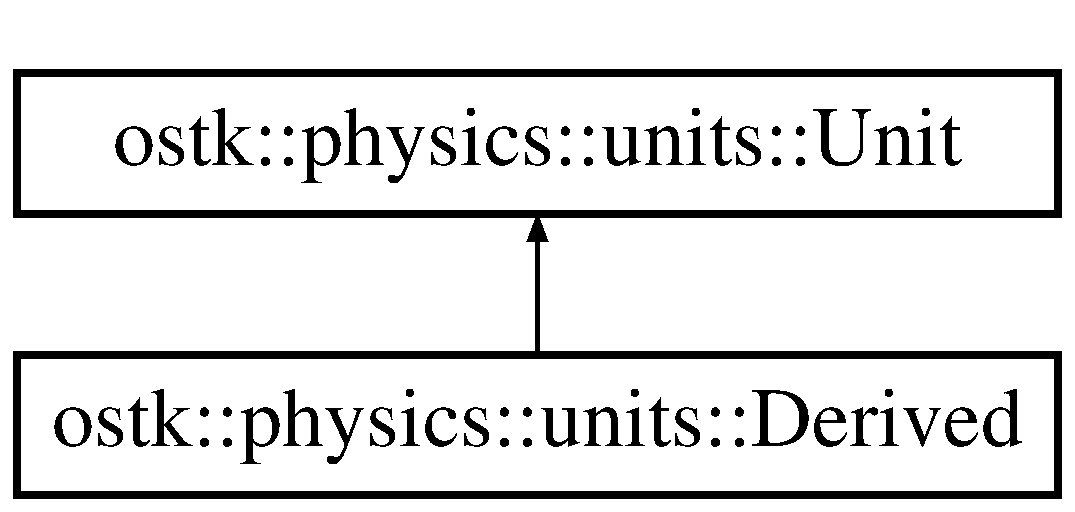
\includegraphics[height=2.000000cm]{classostk_1_1physics_1_1units_1_1_derived}
\end{center}
\end{figure}
\subsection*{Classes}
\begin{DoxyCompactItemize}
\item 
class \hyperlink{classostk_1_1physics_1_1units_1_1_derived_1_1_order}{Order}
\begin{DoxyCompactList}\small\item\em SI unit order. \end{DoxyCompactList}\item 
class \hyperlink{classostk_1_1physics_1_1units_1_1_derived_1_1_unit}{Unit}
\begin{DoxyCompactList}\small\item\em \hyperlink{classostk_1_1physics_1_1units_1_1_derived_1_1_unit}{Unit}. \end{DoxyCompactList}\end{DoxyCompactItemize}
\subsection*{Public Member Functions}
\begin{DoxyCompactItemize}
\item 
\hyperlink{classostk_1_1physics_1_1units_1_1_derived_aa9d64e31cb0027168041184be11b2302}{Derived} (const Real \&a\+Value, const \hyperlink{classostk_1_1physics_1_1units_1_1_derived_1_1_unit}{Derived\+::\+Unit} \&a\+Unit)
\begin{DoxyCompactList}\small\item\em Constructor. \end{DoxyCompactList}\item 
virtual \hyperlink{classostk_1_1physics_1_1units_1_1_derived}{Derived} $\ast$ \hyperlink{classostk_1_1physics_1_1units_1_1_derived_a72a1ae09398204d52a9078da6d36d9d7}{clone} () const override
\item 
bool \hyperlink{classostk_1_1physics_1_1units_1_1_derived_aa20fcc1af55daf9f79d764e2c3d1f1de}{operator==} (const \hyperlink{classostk_1_1physics_1_1units_1_1_derived}{Derived} \&a\+Derived\+Unit) const
\item 
bool \hyperlink{classostk_1_1physics_1_1units_1_1_derived_a34bdca5b46e49122573c2ecd4b5be924}{operator!=} (const \hyperlink{classostk_1_1physics_1_1units_1_1_derived}{Derived} \&a\+Derived\+Unit) const
\item 
virtual bool \hyperlink{classostk_1_1physics_1_1units_1_1_derived_a4221766463c2f4ab478e4a882239eec6}{is\+Defined} () const override
\item 
\hyperlink{classostk_1_1physics_1_1units_1_1_derived_1_1_unit}{Derived\+::\+Unit} \hyperlink{classostk_1_1physics_1_1units_1_1_derived_a85c20f407e3a92bc36f6dbed74cea8bd}{get\+Unit} () const
\item 
Real \hyperlink{classostk_1_1physics_1_1units_1_1_derived_a92880cfa414ae662b754493e9341c5a1}{in} (const \hyperlink{classostk_1_1physics_1_1units_1_1_derived_1_1_unit}{Derived\+::\+Unit} \&a\+Unit) const
\item 
virtual String \hyperlink{classostk_1_1physics_1_1units_1_1_derived_ac1794677978fba5582fb127e032f7398}{to\+String} (const Integer \&a\+Precision=Integer\+::\+Undefined()) const override
\end{DoxyCompactItemize}
\subsection*{Static Public Member Functions}
\begin{DoxyCompactItemize}
\item 
static \hyperlink{classostk_1_1physics_1_1units_1_1_derived}{Derived} \hyperlink{classostk_1_1physics_1_1units_1_1_derived_ada49644ef5ef4de36a257fc7b29505ea}{Undefined} ()
\item 
static \hyperlink{classostk_1_1physics_1_1units_1_1_derived}{Derived} \hyperlink{classostk_1_1physics_1_1units_1_1_derived_acc162f19b9d693c4a24098134a2962db}{Parse} (const String \&a\+String)
\item 
static String \hyperlink{classostk_1_1physics_1_1units_1_1_derived_aaa187a7a568772d01109028aca4cd1a1}{String\+From\+Unit} (const \hyperlink{classostk_1_1physics_1_1units_1_1_derived_1_1_unit}{Derived\+::\+Unit} \&a\+Unit)
\item 
static String \hyperlink{classostk_1_1physics_1_1units_1_1_derived_afd7f7eb95f1de5ca792b587ece5ad3c0}{Symbol\+From\+Unit} (const \hyperlink{classostk_1_1physics_1_1units_1_1_derived_1_1_unit}{Derived\+::\+Unit} \&a\+Unit)
\end{DoxyCompactItemize}
\subsection*{Friends}
\begin{DoxyCompactItemize}
\item 
std\+::ostream \& \hyperlink{classostk_1_1physics_1_1units_1_1_derived_a033deb6664987f4b2f86f5abeb18da81}{operator$<$$<$} (std\+::ostream \&an\+Output\+Stream, const \hyperlink{classostk_1_1physics_1_1units_1_1_derived}{Derived} \&a\+Derived\+Unit)
\end{DoxyCompactItemize}
\subsection*{Additional Inherited Members}


\subsection{Detailed Description}
\hyperlink{classostk_1_1physics_1_1units_1_1_derived}{Derived} unit. 

https\+://en.wikipedia.\+org/wiki/\+S\+I\+\_\+derived\+\_\+unit 

\subsection{Constructor \& Destructor Documentation}
\mbox{\Hypertarget{classostk_1_1physics_1_1units_1_1_derived_aa9d64e31cb0027168041184be11b2302}\label{classostk_1_1physics_1_1units_1_1_derived_aa9d64e31cb0027168041184be11b2302}} 
\index{ostk\+::physics\+::units\+::\+Derived@{ostk\+::physics\+::units\+::\+Derived}!Derived@{Derived}}
\index{Derived@{Derived}!ostk\+::physics\+::units\+::\+Derived@{ostk\+::physics\+::units\+::\+Derived}}
\subsubsection{\texorpdfstring{Derived()}{Derived()}}
{\footnotesize\ttfamily ostk\+::physics\+::units\+::\+Derived\+::\+Derived (\begin{DoxyParamCaption}\item[{const Real \&}]{a\+Value,  }\item[{const \hyperlink{classostk_1_1physics_1_1units_1_1_derived_1_1_unit}{Derived\+::\+Unit} \&}]{a\+Unit }\end{DoxyParamCaption})}



Constructor. 


\begin{DoxyCode}
\end{DoxyCode}



\begin{DoxyParams}[1]{Parameters}
\mbox{\tt in}  & {\em } & \\
\hline
\end{DoxyParams}


\subsection{Member Function Documentation}
\mbox{\Hypertarget{classostk_1_1physics_1_1units_1_1_derived_a72a1ae09398204d52a9078da6d36d9d7}\label{classostk_1_1physics_1_1units_1_1_derived_a72a1ae09398204d52a9078da6d36d9d7}} 
\index{ostk\+::physics\+::units\+::\+Derived@{ostk\+::physics\+::units\+::\+Derived}!clone@{clone}}
\index{clone@{clone}!ostk\+::physics\+::units\+::\+Derived@{ostk\+::physics\+::units\+::\+Derived}}
\subsubsection{\texorpdfstring{clone()}{clone()}}
{\footnotesize\ttfamily \hyperlink{classostk_1_1physics_1_1units_1_1_derived}{Derived} $\ast$ ostk\+::physics\+::units\+::\+Derived\+::clone (\begin{DoxyParamCaption}{ }\end{DoxyParamCaption}) const\hspace{0.3cm}{\ttfamily [override]}, {\ttfamily [virtual]}}



Implements \hyperlink{classostk_1_1physics_1_1units_1_1_unit_ab203628f8a16b16c28d89eaa4c3aff67}{ostk\+::physics\+::units\+::\+Unit}.

\mbox{\Hypertarget{classostk_1_1physics_1_1units_1_1_derived_a85c20f407e3a92bc36f6dbed74cea8bd}\label{classostk_1_1physics_1_1units_1_1_derived_a85c20f407e3a92bc36f6dbed74cea8bd}} 
\index{ostk\+::physics\+::units\+::\+Derived@{ostk\+::physics\+::units\+::\+Derived}!get\+Unit@{get\+Unit}}
\index{get\+Unit@{get\+Unit}!ostk\+::physics\+::units\+::\+Derived@{ostk\+::physics\+::units\+::\+Derived}}
\subsubsection{\texorpdfstring{get\+Unit()}{getUnit()}}
{\footnotesize\ttfamily \hyperlink{classostk_1_1physics_1_1units_1_1_derived_1_1_unit}{Derived\+::\+Unit} ostk\+::physics\+::units\+::\+Derived\+::get\+Unit (\begin{DoxyParamCaption}{ }\end{DoxyParamCaption}) const}

\mbox{\Hypertarget{classostk_1_1physics_1_1units_1_1_derived_a92880cfa414ae662b754493e9341c5a1}\label{classostk_1_1physics_1_1units_1_1_derived_a92880cfa414ae662b754493e9341c5a1}} 
\index{ostk\+::physics\+::units\+::\+Derived@{ostk\+::physics\+::units\+::\+Derived}!in@{in}}
\index{in@{in}!ostk\+::physics\+::units\+::\+Derived@{ostk\+::physics\+::units\+::\+Derived}}
\subsubsection{\texorpdfstring{in()}{in()}}
{\footnotesize\ttfamily Real ostk\+::physics\+::units\+::\+Derived\+::in (\begin{DoxyParamCaption}\item[{const \hyperlink{classostk_1_1physics_1_1units_1_1_derived_1_1_unit}{Derived\+::\+Unit} \&}]{a\+Unit }\end{DoxyParamCaption}) const}

\mbox{\Hypertarget{classostk_1_1physics_1_1units_1_1_derived_a4221766463c2f4ab478e4a882239eec6}\label{classostk_1_1physics_1_1units_1_1_derived_a4221766463c2f4ab478e4a882239eec6}} 
\index{ostk\+::physics\+::units\+::\+Derived@{ostk\+::physics\+::units\+::\+Derived}!is\+Defined@{is\+Defined}}
\index{is\+Defined@{is\+Defined}!ostk\+::physics\+::units\+::\+Derived@{ostk\+::physics\+::units\+::\+Derived}}
\subsubsection{\texorpdfstring{is\+Defined()}{isDefined()}}
{\footnotesize\ttfamily bool ostk\+::physics\+::units\+::\+Derived\+::is\+Defined (\begin{DoxyParamCaption}{ }\end{DoxyParamCaption}) const\hspace{0.3cm}{\ttfamily [override]}, {\ttfamily [virtual]}}



Reimplemented from \hyperlink{classostk_1_1physics_1_1units_1_1_unit_a423ce1df3478f0892b10824b591ae1cc}{ostk\+::physics\+::units\+::\+Unit}.

\mbox{\Hypertarget{classostk_1_1physics_1_1units_1_1_derived_a34bdca5b46e49122573c2ecd4b5be924}\label{classostk_1_1physics_1_1units_1_1_derived_a34bdca5b46e49122573c2ecd4b5be924}} 
\index{ostk\+::physics\+::units\+::\+Derived@{ostk\+::physics\+::units\+::\+Derived}!operator"!=@{operator"!=}}
\index{operator"!=@{operator"!=}!ostk\+::physics\+::units\+::\+Derived@{ostk\+::physics\+::units\+::\+Derived}}
\subsubsection{\texorpdfstring{operator"!=()}{operator!=()}}
{\footnotesize\ttfamily bool ostk\+::physics\+::units\+::\+Derived\+::operator!= (\begin{DoxyParamCaption}\item[{const \hyperlink{classostk_1_1physics_1_1units_1_1_derived}{Derived} \&}]{a\+Derived\+Unit }\end{DoxyParamCaption}) const}

\mbox{\Hypertarget{classostk_1_1physics_1_1units_1_1_derived_aa20fcc1af55daf9f79d764e2c3d1f1de}\label{classostk_1_1physics_1_1units_1_1_derived_aa20fcc1af55daf9f79d764e2c3d1f1de}} 
\index{ostk\+::physics\+::units\+::\+Derived@{ostk\+::physics\+::units\+::\+Derived}!operator==@{operator==}}
\index{operator==@{operator==}!ostk\+::physics\+::units\+::\+Derived@{ostk\+::physics\+::units\+::\+Derived}}
\subsubsection{\texorpdfstring{operator==()}{operator==()}}
{\footnotesize\ttfamily bool ostk\+::physics\+::units\+::\+Derived\+::operator== (\begin{DoxyParamCaption}\item[{const \hyperlink{classostk_1_1physics_1_1units_1_1_derived}{Derived} \&}]{a\+Derived\+Unit }\end{DoxyParamCaption}) const}

\mbox{\Hypertarget{classostk_1_1physics_1_1units_1_1_derived_acc162f19b9d693c4a24098134a2962db}\label{classostk_1_1physics_1_1units_1_1_derived_acc162f19b9d693c4a24098134a2962db}} 
\index{ostk\+::physics\+::units\+::\+Derived@{ostk\+::physics\+::units\+::\+Derived}!Parse@{Parse}}
\index{Parse@{Parse}!ostk\+::physics\+::units\+::\+Derived@{ostk\+::physics\+::units\+::\+Derived}}
\subsubsection{\texorpdfstring{Parse()}{Parse()}}
{\footnotesize\ttfamily static \hyperlink{classostk_1_1physics_1_1units_1_1_derived}{Derived} ostk\+::physics\+::units\+::\+Derived\+::\+Parse (\begin{DoxyParamCaption}\item[{const String \&}]{a\+String }\end{DoxyParamCaption})\hspace{0.3cm}{\ttfamily [static]}}

\mbox{\Hypertarget{classostk_1_1physics_1_1units_1_1_derived_aaa187a7a568772d01109028aca4cd1a1}\label{classostk_1_1physics_1_1units_1_1_derived_aaa187a7a568772d01109028aca4cd1a1}} 
\index{ostk\+::physics\+::units\+::\+Derived@{ostk\+::physics\+::units\+::\+Derived}!String\+From\+Unit@{String\+From\+Unit}}
\index{String\+From\+Unit@{String\+From\+Unit}!ostk\+::physics\+::units\+::\+Derived@{ostk\+::physics\+::units\+::\+Derived}}
\subsubsection{\texorpdfstring{String\+From\+Unit()}{StringFromUnit()}}
{\footnotesize\ttfamily String ostk\+::physics\+::units\+::\+Derived\+::\+String\+From\+Unit (\begin{DoxyParamCaption}\item[{const \hyperlink{classostk_1_1physics_1_1units_1_1_derived_1_1_unit}{Derived\+::\+Unit} \&}]{a\+Unit }\end{DoxyParamCaption})\hspace{0.3cm}{\ttfamily [static]}}

\mbox{\Hypertarget{classostk_1_1physics_1_1units_1_1_derived_afd7f7eb95f1de5ca792b587ece5ad3c0}\label{classostk_1_1physics_1_1units_1_1_derived_afd7f7eb95f1de5ca792b587ece5ad3c0}} 
\index{ostk\+::physics\+::units\+::\+Derived@{ostk\+::physics\+::units\+::\+Derived}!Symbol\+From\+Unit@{Symbol\+From\+Unit}}
\index{Symbol\+From\+Unit@{Symbol\+From\+Unit}!ostk\+::physics\+::units\+::\+Derived@{ostk\+::physics\+::units\+::\+Derived}}
\subsubsection{\texorpdfstring{Symbol\+From\+Unit()}{SymbolFromUnit()}}
{\footnotesize\ttfamily String ostk\+::physics\+::units\+::\+Derived\+::\+Symbol\+From\+Unit (\begin{DoxyParamCaption}\item[{const \hyperlink{classostk_1_1physics_1_1units_1_1_derived_1_1_unit}{Derived\+::\+Unit} \&}]{a\+Unit }\end{DoxyParamCaption})\hspace{0.3cm}{\ttfamily [static]}}

\mbox{\Hypertarget{classostk_1_1physics_1_1units_1_1_derived_ac1794677978fba5582fb127e032f7398}\label{classostk_1_1physics_1_1units_1_1_derived_ac1794677978fba5582fb127e032f7398}} 
\index{ostk\+::physics\+::units\+::\+Derived@{ostk\+::physics\+::units\+::\+Derived}!to\+String@{to\+String}}
\index{to\+String@{to\+String}!ostk\+::physics\+::units\+::\+Derived@{ostk\+::physics\+::units\+::\+Derived}}
\subsubsection{\texorpdfstring{to\+String()}{toString()}}
{\footnotesize\ttfamily String ostk\+::physics\+::units\+::\+Derived\+::to\+String (\begin{DoxyParamCaption}\item[{const Integer \&}]{a\+Precision = {\ttfamily Integer\+:\+:Undefined()} }\end{DoxyParamCaption}) const\hspace{0.3cm}{\ttfamily [override]}, {\ttfamily [virtual]}}



Implements \hyperlink{classostk_1_1physics_1_1units_1_1_unit_a8162b4eb8221c7577af16ab8b399d07e}{ostk\+::physics\+::units\+::\+Unit}.

\mbox{\Hypertarget{classostk_1_1physics_1_1units_1_1_derived_ada49644ef5ef4de36a257fc7b29505ea}\label{classostk_1_1physics_1_1units_1_1_derived_ada49644ef5ef4de36a257fc7b29505ea}} 
\index{ostk\+::physics\+::units\+::\+Derived@{ostk\+::physics\+::units\+::\+Derived}!Undefined@{Undefined}}
\index{Undefined@{Undefined}!ostk\+::physics\+::units\+::\+Derived@{ostk\+::physics\+::units\+::\+Derived}}
\subsubsection{\texorpdfstring{Undefined()}{Undefined()}}
{\footnotesize\ttfamily \hyperlink{classostk_1_1physics_1_1units_1_1_derived}{Derived} ostk\+::physics\+::units\+::\+Derived\+::\+Undefined (\begin{DoxyParamCaption}{ }\end{DoxyParamCaption})\hspace{0.3cm}{\ttfamily [static]}}



\subsection{Friends And Related Function Documentation}
\mbox{\Hypertarget{classostk_1_1physics_1_1units_1_1_derived_a033deb6664987f4b2f86f5abeb18da81}\label{classostk_1_1physics_1_1units_1_1_derived_a033deb6664987f4b2f86f5abeb18da81}} 
\index{ostk\+::physics\+::units\+::\+Derived@{ostk\+::physics\+::units\+::\+Derived}!operator$<$$<$@{operator$<$$<$}}
\index{operator$<$$<$@{operator$<$$<$}!ostk\+::physics\+::units\+::\+Derived@{ostk\+::physics\+::units\+::\+Derived}}
\subsubsection{\texorpdfstring{operator$<$$<$}{operator<<}}
{\footnotesize\ttfamily std\+::ostream\& operator$<$$<$ (\begin{DoxyParamCaption}\item[{std\+::ostream \&}]{an\+Output\+Stream,  }\item[{const \hyperlink{classostk_1_1physics_1_1units_1_1_derived}{Derived} \&}]{a\+Derived\+Unit }\end{DoxyParamCaption})\hspace{0.3cm}{\ttfamily [friend]}}



The documentation for this class was generated from the following files\+:\begin{DoxyCompactItemize}
\item 
include/\+Open\+Space\+Toolkit/\+Physics/\+Units/\hyperlink{_derived_8hpp}{Derived.\+hpp}\item 
src/\+Open\+Space\+Toolkit/\+Physics/\+Units/\hyperlink{_derived_8cpp}{Derived.\+cpp}\end{DoxyCompactItemize}

\hypertarget{classostk_1_1physics_1_1environment_1_1magnetic_1_1_dipole}{}\section{ostk\+:\+:physics\+:\+:environment\+:\+:magnetic\+:\+:Dipole Class Reference}
\label{classostk_1_1physics_1_1environment_1_1magnetic_1_1_dipole}\index{ostk\+::physics\+::environment\+::magnetic\+::\+Dipole@{ostk\+::physics\+::environment\+::magnetic\+::\+Dipole}}


Magnetic dipole model.  




{\ttfamily \#include $<$Dipole.\+hpp$>$}

Inheritance diagram for ostk\+:\+:physics\+:\+:environment\+:\+:magnetic\+:\+:Dipole\+:\begin{figure}[H]
\begin{center}
\leavevmode
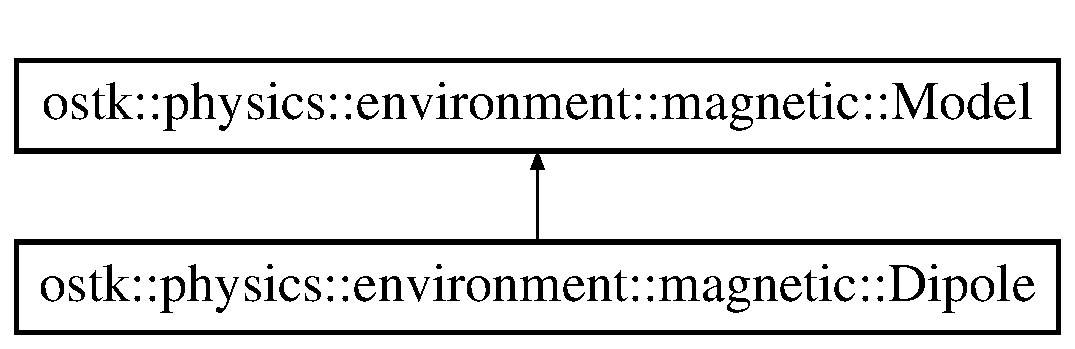
\includegraphics[height=2.000000cm]{classostk_1_1physics_1_1environment_1_1magnetic_1_1_dipole}
\end{center}
\end{figure}
\subsection*{Public Member Functions}
\begin{DoxyCompactItemize}
\item 
\hyperlink{classostk_1_1physics_1_1environment_1_1magnetic_1_1_dipole_a974e9a8c1062516d6c872b96d5573779}{Dipole} (const Vector3d \&a\+Magnetic\+Moment)
\begin{DoxyCompactList}\small\item\em Constructor. \end{DoxyCompactList}\item 
virtual \hyperlink{classostk_1_1physics_1_1environment_1_1magnetic_1_1_dipole}{Dipole} $\ast$ \hyperlink{classostk_1_1physics_1_1environment_1_1magnetic_1_1_dipole_ad4255ff1007a339c9f0bdbda321c0ab2}{clone} () const override
\begin{DoxyCompactList}\small\item\em Clone the dipole magnetic model. \end{DoxyCompactList}\item 
virtual Vector3d \hyperlink{classostk_1_1physics_1_1environment_1_1magnetic_1_1_dipole_ae2c65e41445c91b3efec455fb5077ab1}{get\+Field\+Value\+At} (const Vector3d \&a\+Position, const \hyperlink{classostk_1_1physics_1_1time_1_1_instant}{Instant} \&an\+Instant) const override
\begin{DoxyCompactList}\small\item\em Get the magnetic field value at a given position and instant. \end{DoxyCompactList}\end{DoxyCompactItemize}


\subsection{Detailed Description}
Magnetic dipole model. 

https\+://en.wikipedia.\+org/wiki/\+Magnetic\+\_\+dipole https\+://en.wikipedia.\+org/wiki/\+Magnetic\+\_\+moment https\+://en.wikipedia.\+org/wiki/\+Vacuum\+\_\+permeability https\+://en.wikipedia.\+org/wiki/\+Dipole\+\_\+model\+\_\+of\+\_\+the\+\_\+\+Earth\%27s\+\_\+magnetic\+\_\+field 

\subsection{Constructor \& Destructor Documentation}
\mbox{\Hypertarget{classostk_1_1physics_1_1environment_1_1magnetic_1_1_dipole_a974e9a8c1062516d6c872b96d5573779}\label{classostk_1_1physics_1_1environment_1_1magnetic_1_1_dipole_a974e9a8c1062516d6c872b96d5573779}} 
\index{ostk\+::physics\+::environment\+::magnetic\+::\+Dipole@{ostk\+::physics\+::environment\+::magnetic\+::\+Dipole}!Dipole@{Dipole}}
\index{Dipole@{Dipole}!ostk\+::physics\+::environment\+::magnetic\+::\+Dipole@{ostk\+::physics\+::environment\+::magnetic\+::\+Dipole}}
\subsubsection{\texorpdfstring{Dipole()}{Dipole()}}
{\footnotesize\ttfamily ostk\+::physics\+::environment\+::magnetic\+::\+Dipole\+::\+Dipole (\begin{DoxyParamCaption}\item[{const Vector3d \&}]{a\+Magnetic\+Moment }\end{DoxyParamCaption})}



Constructor. 


\begin{DoxyParams}[1]{Parameters}
\mbox{\tt in}  & {\em a\+Magnetic\+Moment} & A magnetic moment \mbox{[}A⋅m2\mbox{]} \\
\hline
\end{DoxyParams}


\subsection{Member Function Documentation}
\mbox{\Hypertarget{classostk_1_1physics_1_1environment_1_1magnetic_1_1_dipole_ad4255ff1007a339c9f0bdbda321c0ab2}\label{classostk_1_1physics_1_1environment_1_1magnetic_1_1_dipole_ad4255ff1007a339c9f0bdbda321c0ab2}} 
\index{ostk\+::physics\+::environment\+::magnetic\+::\+Dipole@{ostk\+::physics\+::environment\+::magnetic\+::\+Dipole}!clone@{clone}}
\index{clone@{clone}!ostk\+::physics\+::environment\+::magnetic\+::\+Dipole@{ostk\+::physics\+::environment\+::magnetic\+::\+Dipole}}
\subsubsection{\texorpdfstring{clone()}{clone()}}
{\footnotesize\ttfamily \hyperlink{classostk_1_1physics_1_1environment_1_1magnetic_1_1_dipole}{Dipole} $\ast$ ostk\+::physics\+::environment\+::magnetic\+::\+Dipole\+::clone (\begin{DoxyParamCaption}{ }\end{DoxyParamCaption}) const\hspace{0.3cm}{\ttfamily [override]}, {\ttfamily [virtual]}}



Clone the dipole magnetic model. 

\begin{DoxyReturn}{Returns}
Pointer to dipole magnetic model 
\end{DoxyReturn}


Implements \hyperlink{classostk_1_1physics_1_1environment_1_1magnetic_1_1_model_af357908c151a7809bbbc8fc676bd07b6}{ostk\+::physics\+::environment\+::magnetic\+::\+Model}.

\mbox{\Hypertarget{classostk_1_1physics_1_1environment_1_1magnetic_1_1_dipole_ae2c65e41445c91b3efec455fb5077ab1}\label{classostk_1_1physics_1_1environment_1_1magnetic_1_1_dipole_ae2c65e41445c91b3efec455fb5077ab1}} 
\index{ostk\+::physics\+::environment\+::magnetic\+::\+Dipole@{ostk\+::physics\+::environment\+::magnetic\+::\+Dipole}!get\+Field\+Value\+At@{get\+Field\+Value\+At}}
\index{get\+Field\+Value\+At@{get\+Field\+Value\+At}!ostk\+::physics\+::environment\+::magnetic\+::\+Dipole@{ostk\+::physics\+::environment\+::magnetic\+::\+Dipole}}
\subsubsection{\texorpdfstring{get\+Field\+Value\+At()}{getFieldValueAt()}}
{\footnotesize\ttfamily Vector3d ostk\+::physics\+::environment\+::magnetic\+::\+Dipole\+::get\+Field\+Value\+At (\begin{DoxyParamCaption}\item[{const Vector3d \&}]{a\+Position,  }\item[{const \hyperlink{classostk_1_1physics_1_1time_1_1_instant}{Instant} \&}]{an\+Instant }\end{DoxyParamCaption}) const\hspace{0.3cm}{\ttfamily [override]}, {\ttfamily [virtual]}}



Get the magnetic field value at a given position and instant. 


\begin{DoxyParams}[1]{Parameters}
\mbox{\tt in}  & {\em a\+Position} & A position, expressed in the magnetic object frame \mbox{[}m\mbox{]} \\
\hline
\mbox{\tt in}  & {\em an\+Instant} & An instant \\
\hline
\end{DoxyParams}
\begin{DoxyReturn}{Returns}
Magnetic field value, expressed in the magnetic object frame \mbox{[}T\mbox{]} 
\end{DoxyReturn}


Implements \hyperlink{classostk_1_1physics_1_1environment_1_1magnetic_1_1_model_abf0510f9be2c196ea3c0586d02979b0f}{ostk\+::physics\+::environment\+::magnetic\+::\+Model}.



The documentation for this class was generated from the following files\+:\begin{DoxyCompactItemize}
\item 
include/\+Open\+Space\+Toolkit/\+Physics/\+Environment/\+Magnetic/\hyperlink{_dipole_8hpp}{Dipole.\+hpp}\item 
src/\+Open\+Space\+Toolkit/\+Physics/\+Environment/\+Magnetic/\hyperlink{_dipole_8cpp}{Dipole.\+cpp}\end{DoxyCompactItemize}

\hypertarget{classostk_1_1physics_1_1data_1_1_direction}{}\section{ostk\+:\+:physics\+:\+:data\+:\+:Direction Class Reference}
\label{classostk_1_1physics_1_1data_1_1_direction}\index{ostk\+::physics\+::data\+::\+Direction@{ostk\+::physics\+::data\+::\+Direction}}


\hyperlink{classostk_1_1physics_1_1data_1_1_direction}{Direction}.  




{\ttfamily \#include $<$Direction.\+hpp$>$}

Inheritance diagram for ostk\+:\+:physics\+:\+:data\+:\+:Direction\+:\begin{figure}[H]
\begin{center}
\leavevmode
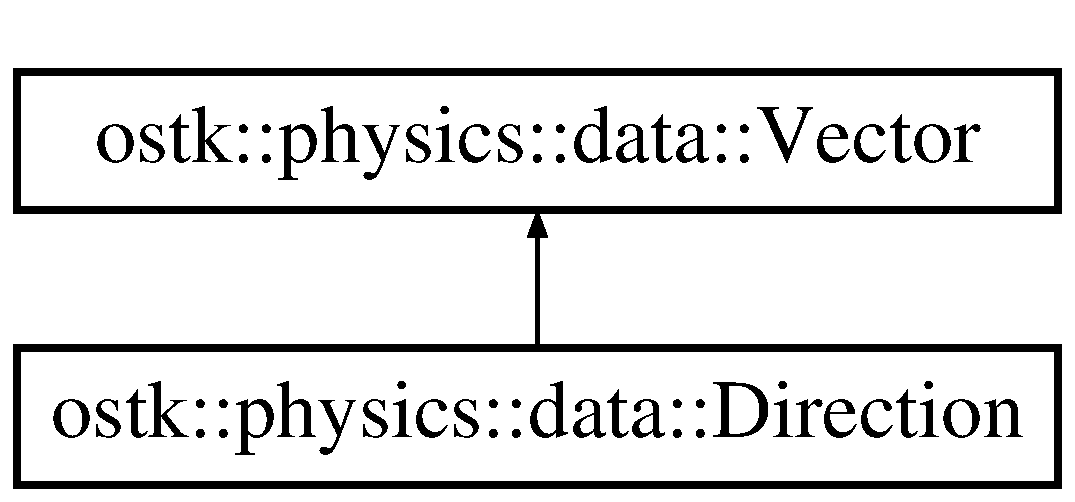
\includegraphics[height=2.000000cm]{classostk_1_1physics_1_1data_1_1_direction}
\end{center}
\end{figure}
\subsection*{Public Member Functions}
\begin{DoxyCompactItemize}
\item 
\hyperlink{classostk_1_1physics_1_1data_1_1_direction_ac247d7c6d290db488940c0100b5cda5d}{Direction} (const Vector3d \&a\+Value, const Shared$<$ const \hyperlink{classostk_1_1physics_1_1coord_1_1_frame}{Frame} $>$ \&a\+Frame\+S\+Ptr)
\item 
bool \hyperlink{classostk_1_1physics_1_1data_1_1_direction_aa1d684ca3528113e412f9d8b5d51b49f}{operator==} (const \hyperlink{classostk_1_1physics_1_1data_1_1_direction}{Direction} \&a\+Direction) const
\item 
bool \hyperlink{classostk_1_1physics_1_1data_1_1_direction_a90bf1d390562e9b3a8115af07b6b4e6b}{operator!=} (const \hyperlink{classostk_1_1physics_1_1data_1_1_direction}{Direction} \&a\+Direction) const
\end{DoxyCompactItemize}
\subsection*{Static Public Member Functions}
\begin{DoxyCompactItemize}
\item 
static \hyperlink{classostk_1_1physics_1_1data_1_1_direction}{Direction} \hyperlink{classostk_1_1physics_1_1data_1_1_direction_a47b0ba9fb3f592e2fd1fba846af6483c}{Undefined} ()
\end{DoxyCompactItemize}
\subsection*{Friends}
\begin{DoxyCompactItemize}
\item 
std\+::ostream \& \hyperlink{classostk_1_1physics_1_1data_1_1_direction_a2f1253dbad20965d2209456421eabf71}{operator$<$$<$} (std\+::ostream \&an\+Output\+Stream, const \hyperlink{classostk_1_1physics_1_1data_1_1_vector}{Vector} \&a\+Vector)
\end{DoxyCompactItemize}


\subsection{Detailed Description}
\hyperlink{classostk_1_1physics_1_1data_1_1_direction}{Direction}. 

A unit vector, expressed in a given frame. 

\subsection{Constructor \& Destructor Documentation}
\mbox{\Hypertarget{classostk_1_1physics_1_1data_1_1_direction_ac247d7c6d290db488940c0100b5cda5d}\label{classostk_1_1physics_1_1data_1_1_direction_ac247d7c6d290db488940c0100b5cda5d}} 
\index{ostk\+::physics\+::data\+::\+Direction@{ostk\+::physics\+::data\+::\+Direction}!Direction@{Direction}}
\index{Direction@{Direction}!ostk\+::physics\+::data\+::\+Direction@{ostk\+::physics\+::data\+::\+Direction}}
\subsubsection{\texorpdfstring{Direction()}{Direction()}}
{\footnotesize\ttfamily ostk\+::physics\+::data\+::\+Direction\+::\+Direction (\begin{DoxyParamCaption}\item[{const Vector3d \&}]{a\+Value,  }\item[{const Shared$<$ const \hyperlink{classostk_1_1physics_1_1coord_1_1_frame}{Frame} $>$ \&}]{a\+Frame\+S\+Ptr }\end{DoxyParamCaption})}



\subsection{Member Function Documentation}
\mbox{\Hypertarget{classostk_1_1physics_1_1data_1_1_direction_a90bf1d390562e9b3a8115af07b6b4e6b}\label{classostk_1_1physics_1_1data_1_1_direction_a90bf1d390562e9b3a8115af07b6b4e6b}} 
\index{ostk\+::physics\+::data\+::\+Direction@{ostk\+::physics\+::data\+::\+Direction}!operator"!=@{operator"!=}}
\index{operator"!=@{operator"!=}!ostk\+::physics\+::data\+::\+Direction@{ostk\+::physics\+::data\+::\+Direction}}
\subsubsection{\texorpdfstring{operator"!=()}{operator!=()}}
{\footnotesize\ttfamily bool ostk\+::physics\+::data\+::\+Direction\+::operator!= (\begin{DoxyParamCaption}\item[{const \hyperlink{classostk_1_1physics_1_1data_1_1_direction}{Direction} \&}]{a\+Direction }\end{DoxyParamCaption}) const}

\mbox{\Hypertarget{classostk_1_1physics_1_1data_1_1_direction_aa1d684ca3528113e412f9d8b5d51b49f}\label{classostk_1_1physics_1_1data_1_1_direction_aa1d684ca3528113e412f9d8b5d51b49f}} 
\index{ostk\+::physics\+::data\+::\+Direction@{ostk\+::physics\+::data\+::\+Direction}!operator==@{operator==}}
\index{operator==@{operator==}!ostk\+::physics\+::data\+::\+Direction@{ostk\+::physics\+::data\+::\+Direction}}
\subsubsection{\texorpdfstring{operator==()}{operator==()}}
{\footnotesize\ttfamily bool ostk\+::physics\+::data\+::\+Direction\+::operator== (\begin{DoxyParamCaption}\item[{const \hyperlink{classostk_1_1physics_1_1data_1_1_direction}{Direction} \&}]{a\+Direction }\end{DoxyParamCaption}) const}

\mbox{\Hypertarget{classostk_1_1physics_1_1data_1_1_direction_a47b0ba9fb3f592e2fd1fba846af6483c}\label{classostk_1_1physics_1_1data_1_1_direction_a47b0ba9fb3f592e2fd1fba846af6483c}} 
\index{ostk\+::physics\+::data\+::\+Direction@{ostk\+::physics\+::data\+::\+Direction}!Undefined@{Undefined}}
\index{Undefined@{Undefined}!ostk\+::physics\+::data\+::\+Direction@{ostk\+::physics\+::data\+::\+Direction}}
\subsubsection{\texorpdfstring{Undefined()}{Undefined()}}
{\footnotesize\ttfamily \hyperlink{classostk_1_1physics_1_1data_1_1_direction}{Direction} ostk\+::physics\+::data\+::\+Direction\+::\+Undefined (\begin{DoxyParamCaption}{ }\end{DoxyParamCaption})\hspace{0.3cm}{\ttfamily [static]}}



\subsection{Friends And Related Function Documentation}
\mbox{\Hypertarget{classostk_1_1physics_1_1data_1_1_direction_a2f1253dbad20965d2209456421eabf71}\label{classostk_1_1physics_1_1data_1_1_direction_a2f1253dbad20965d2209456421eabf71}} 
\index{ostk\+::physics\+::data\+::\+Direction@{ostk\+::physics\+::data\+::\+Direction}!operator$<$$<$@{operator$<$$<$}}
\index{operator$<$$<$@{operator$<$$<$}!ostk\+::physics\+::data\+::\+Direction@{ostk\+::physics\+::data\+::\+Direction}}
\subsubsection{\texorpdfstring{operator$<$$<$}{operator<<}}
{\footnotesize\ttfamily std\+::ostream\& operator$<$$<$ (\begin{DoxyParamCaption}\item[{std\+::ostream \&}]{an\+Output\+Stream,  }\item[{const \hyperlink{classostk_1_1physics_1_1data_1_1_vector}{Vector} \&}]{a\+Vector }\end{DoxyParamCaption})\hspace{0.3cm}{\ttfamily [friend]}}



The documentation for this class was generated from the following files\+:\begin{DoxyCompactItemize}
\item 
include/\+Open\+Space\+Toolkit/\+Physics/\+Data/\hyperlink{_direction_8hpp}{Direction.\+hpp}\item 
src/\+Open\+Space\+Toolkit/\+Physics/\+Data/\hyperlink{_direction_8cpp}{Direction.\+cpp}\end{DoxyCompactItemize}

\hypertarget{classostk_1_1physics_1_1time_1_1_duration}{}\section{ostk\+:\+:physics\+:\+:time\+:\+:Duration Class Reference}
\label{classostk_1_1physics_1_1time_1_1_duration}\index{ostk\+::physics\+::time\+::\+Duration@{ostk\+::physics\+::time\+::\+Duration}}


Amount of time.  




{\ttfamily \#include $<$Duration.\+hpp$>$}

\subsection*{Public Types}
\begin{DoxyCompactItemize}
\item 
enum \hyperlink{classostk_1_1physics_1_1time_1_1_duration_a4bf616b67d15e0fbc4beb4fcc306c368}{Format} \{ \hyperlink{classostk_1_1physics_1_1time_1_1_duration_a4bf616b67d15e0fbc4beb4fcc306c368aec0fc0100c4fc1ce4eea230c3dc10360}{Format\+::\+Undefined}, 
\hyperlink{classostk_1_1physics_1_1time_1_1_duration_a4bf616b67d15e0fbc4beb4fcc306c368aeb6d8ae6f20283755b339c0dc273988b}{Format\+::\+Standard}, 
\hyperlink{classostk_1_1physics_1_1time_1_1_duration_a4bf616b67d15e0fbc4beb4fcc306c368a35b6786739efcdc5a74ab1dca29d3b6b}{Format\+::\+I\+S\+O8601}
 \}\begin{DoxyCompactList}\small\item\em \hyperlink{classostk_1_1physics_1_1time_1_1_duration}{Duration} format. \end{DoxyCompactList}
\end{DoxyCompactItemize}
\subsection*{Public Member Functions}
\begin{DoxyCompactItemize}
\item 
\hyperlink{classostk_1_1physics_1_1time_1_1_duration_a6ba3a020742ca6e3bf0b1970dd039c07}{Duration} (Int64 a\+Nanosecond\+Count)
\begin{DoxyCompactList}\small\item\em Constructor. \end{DoxyCompactList}\item 
bool \hyperlink{classostk_1_1physics_1_1time_1_1_duration_a92649b4f3f332daf372bb78ac1db6740}{operator==} (const \hyperlink{classostk_1_1physics_1_1time_1_1_duration}{Duration} \&a\+Duration) const
\begin{DoxyCompactList}\small\item\em Equal to operator. \end{DoxyCompactList}\item 
bool \hyperlink{classostk_1_1physics_1_1time_1_1_duration_a5e99b046bbf8aa1de0f8e212b7794e38}{operator!=} (const \hyperlink{classostk_1_1physics_1_1time_1_1_duration}{Duration} \&a\+Duration) const
\begin{DoxyCompactList}\small\item\em Not equal to operator. \end{DoxyCompactList}\item 
bool \hyperlink{classostk_1_1physics_1_1time_1_1_duration_a76fbb444ae7db2e6e61c237bf96b9032}{operator$<$} (const \hyperlink{classostk_1_1physics_1_1time_1_1_duration}{Duration} \&a\+Duration) const
\begin{DoxyCompactList}\small\item\em Less than operator. \end{DoxyCompactList}\item 
bool \hyperlink{classostk_1_1physics_1_1time_1_1_duration_a31b9328d64a66fd3f46ca8100b8dd91c}{operator$<$=} (const \hyperlink{classostk_1_1physics_1_1time_1_1_duration}{Duration} \&a\+Duration) const
\begin{DoxyCompactList}\small\item\em Less than or equal to operator. \end{DoxyCompactList}\item 
bool \hyperlink{classostk_1_1physics_1_1time_1_1_duration_a9daebcdc2a5ab12306630d85e44dcb7a}{operator$>$} (const \hyperlink{classostk_1_1physics_1_1time_1_1_duration}{Duration} \&a\+Duration) const
\begin{DoxyCompactList}\small\item\em Greater than operator. \end{DoxyCompactList}\item 
bool \hyperlink{classostk_1_1physics_1_1time_1_1_duration_a3c742aac8e660effd3575fe0ca570d75}{operator$>$=} (const \hyperlink{classostk_1_1physics_1_1time_1_1_duration}{Duration} \&a\+Duration) const
\begin{DoxyCompactList}\small\item\em Greater than operator. \end{DoxyCompactList}\item 
\hyperlink{classostk_1_1physics_1_1time_1_1_duration}{Duration} \hyperlink{classostk_1_1physics_1_1time_1_1_duration_a26a68103c9ee563c99257590fbc60079}{operator+} (const \hyperlink{classostk_1_1physics_1_1time_1_1_duration}{Duration} \&a\+Duration) const
\begin{DoxyCompactList}\small\item\em Addition operator. \end{DoxyCompactList}\item 
\hyperlink{classostk_1_1physics_1_1time_1_1_duration}{Duration} \hyperlink{classostk_1_1physics_1_1time_1_1_duration_a211f0f909d453c61aad6677409507698}{operator-\/} (const \hyperlink{classostk_1_1physics_1_1time_1_1_duration}{Duration} \&a\+Duration) const
\begin{DoxyCompactList}\small\item\em Subtraction operator. \end{DoxyCompactList}\item 
\hyperlink{classostk_1_1physics_1_1time_1_1_duration}{Duration} \hyperlink{classostk_1_1physics_1_1time_1_1_duration_afca79b9de1ea487b00abdb8be8c5608d}{operator$\ast$} (const Real \&a\+Multiplier) const
\begin{DoxyCompactList}\small\item\em Multiplication operator. \end{DoxyCompactList}\item 
\hyperlink{classostk_1_1physics_1_1time_1_1_duration}{Duration} \hyperlink{classostk_1_1physics_1_1time_1_1_duration_a2400f4ac59f56e2a73090cff9404c67c}{operator/} (const Real \&a\+Divider) const
\begin{DoxyCompactList}\small\item\em Division operator. \end{DoxyCompactList}\item 
\hyperlink{classostk_1_1physics_1_1time_1_1_duration}{Duration} \hyperlink{classostk_1_1physics_1_1time_1_1_duration_a172bf36df42a169ecf5893daa3f7d7b2}{operator+} () const
\begin{DoxyCompactList}\small\item\em Unary plus operator. \end{DoxyCompactList}\item 
\hyperlink{classostk_1_1physics_1_1time_1_1_duration}{Duration} \hyperlink{classostk_1_1physics_1_1time_1_1_duration_ad6311a658bac277c9739cf938106a274}{operator-\/} () const
\begin{DoxyCompactList}\small\item\em Unary minus operator. \end{DoxyCompactList}\item 
\hyperlink{classostk_1_1physics_1_1time_1_1_duration}{Duration} \& \hyperlink{classostk_1_1physics_1_1time_1_1_duration_af0bd86fc4ec2d7a59219b3c72f699892}{operator+=} (const \hyperlink{classostk_1_1physics_1_1time_1_1_duration}{Duration} \&a\+Duration)
\begin{DoxyCompactList}\small\item\em Addition assignement operator. \end{DoxyCompactList}\item 
\hyperlink{classostk_1_1physics_1_1time_1_1_duration}{Duration} \& \hyperlink{classostk_1_1physics_1_1time_1_1_duration_a81655d5bcb4ed4b13d2858a4c01917bd}{operator-\/=} (const \hyperlink{classostk_1_1physics_1_1time_1_1_duration}{Duration} \&a\+Duration)
\begin{DoxyCompactList}\small\item\em Subtraction assignement operator. \end{DoxyCompactList}\item 
\hyperlink{classostk_1_1physics_1_1time_1_1_duration}{Duration} \& \hyperlink{classostk_1_1physics_1_1time_1_1_duration_ae26dc624227d7c6d8cb4a7436c34a4ae}{operator$\ast$=} (const Real \&a\+Multiplier)
\begin{DoxyCompactList}\small\item\em Multiplication assignement operator. \end{DoxyCompactList}\item 
\hyperlink{classostk_1_1physics_1_1time_1_1_duration}{Duration} \& \hyperlink{classostk_1_1physics_1_1time_1_1_duration_ac1e48e49d1dfeb3890a6944f13c513b7}{operator/=} (const Real \&a\+Divider)
\begin{DoxyCompactList}\small\item\em Division assignement operator. \end{DoxyCompactList}\item 
bool \hyperlink{classostk_1_1physics_1_1time_1_1_duration_a4676fb2c4107f121bd197d4475507d40}{is\+Defined} () const
\begin{DoxyCompactList}\small\item\em Check if duration is defined. \end{DoxyCompactList}\item 
bool \hyperlink{classostk_1_1physics_1_1time_1_1_duration_a41b6aa4c574b3b98c32d5fafaa0a1fc2}{is\+Zero} () const
\begin{DoxyCompactList}\small\item\em Check if duration is zero. \end{DoxyCompactList}\item 
bool \hyperlink{classostk_1_1physics_1_1time_1_1_duration_a98211c27882beea4d5eadb6e825b85cb}{is\+Positive} () const
\begin{DoxyCompactList}\small\item\em Check if duration is positive. \end{DoxyCompactList}\item 
bool \hyperlink{classostk_1_1physics_1_1time_1_1_duration_ad72312f690761a3b5bfbe8ed0204d87e}{is\+Strictly\+Positive} () const
\begin{DoxyCompactList}\small\item\em Check if duration is strictly positive. \end{DoxyCompactList}\item 
bool \hyperlink{classostk_1_1physics_1_1time_1_1_duration_a89fe2dee0dec4b81040ecc7a31bb3f87}{is\+Near} (const \hyperlink{classostk_1_1physics_1_1time_1_1_duration}{Duration} \&a\+Duration, const \hyperlink{classostk_1_1physics_1_1time_1_1_duration}{Duration} \&a\+Tolerance) const
\begin{DoxyCompactList}\small\item\em Check if duration is near another duration. \end{DoxyCompactList}\item 
Integer \hyperlink{classostk_1_1physics_1_1time_1_1_duration_a6b5818c374c3535f7827f6970c563206}{get\+Nanoseconds} () const
\begin{DoxyCompactList}\small\item\em Get the number of nanoseconds in duration. \end{DoxyCompactList}\item 
Integer \hyperlink{classostk_1_1physics_1_1time_1_1_duration_a022d05824638f8288e84131d6b5e07be}{get\+Microseconds} () const
\begin{DoxyCompactList}\small\item\em Get the number of microseconds in duration. \end{DoxyCompactList}\item 
Integer \hyperlink{classostk_1_1physics_1_1time_1_1_duration_a4ff289a3d0fb16c73899adcfe381a111}{get\+Milliseconds} () const
\begin{DoxyCompactList}\small\item\em Get the number of milliseconds in duration. \end{DoxyCompactList}\item 
Integer \hyperlink{classostk_1_1physics_1_1time_1_1_duration_aff2319bf58b7c3da9e87ccd88867ffe7}{get\+Seconds} () const
\begin{DoxyCompactList}\small\item\em Get the number of seconds in duration. \end{DoxyCompactList}\item 
Integer \hyperlink{classostk_1_1physics_1_1time_1_1_duration_a59eb18f0275a8683e73b9b86194bf9da}{get\+Minutes} () const
\begin{DoxyCompactList}\small\item\em Get the number of minutes in duration. \end{DoxyCompactList}\item 
Integer \hyperlink{classostk_1_1physics_1_1time_1_1_duration_ac33d36a6a043ad71b0203b02b9ff961b}{get\+Hours} () const
\begin{DoxyCompactList}\small\item\em Get the number of hours in duration. \end{DoxyCompactList}\item 
Integer \hyperlink{classostk_1_1physics_1_1time_1_1_duration_a8902625ed4b1d8d2a23bf7c5e9f886c4}{get\+Days} () const
\begin{DoxyCompactList}\small\item\em Get the number of days in duration. \end{DoxyCompactList}\item 
Integer \hyperlink{classostk_1_1physics_1_1time_1_1_duration_af42d2314c9d99b87ff09cf8470a460cd}{get\+Weeks} () const
\begin{DoxyCompactList}\small\item\em Get the number of weeks in duration. \end{DoxyCompactList}\item 
Real \hyperlink{classostk_1_1physics_1_1time_1_1_duration_a00148c707cda4dc7b93aab5280200cd5}{in\+Nanoseconds} () const
\begin{DoxyCompactList}\small\item\em Get nanosecond count. \end{DoxyCompactList}\item 
Real \hyperlink{classostk_1_1physics_1_1time_1_1_duration_a67a7723ff079f5a4404a5fa1b0fd2128}{in\+Microseconds} () const
\begin{DoxyCompactList}\small\item\em Get microsecond count. \end{DoxyCompactList}\item 
Real \hyperlink{classostk_1_1physics_1_1time_1_1_duration_a8a754e57d49d857d7fbcd62be81b858d}{in\+Milliseconds} () const
\begin{DoxyCompactList}\small\item\em Get millisecond count. \end{DoxyCompactList}\item 
Real \hyperlink{classostk_1_1physics_1_1time_1_1_duration_ab2062045cd441c3eba4d58773a7bb01b}{in\+Seconds} () const
\begin{DoxyCompactList}\small\item\em Get second count. \end{DoxyCompactList}\item 
Real \hyperlink{classostk_1_1physics_1_1time_1_1_duration_a8ad5153d6f3ee225d9e4c32a2e19febc}{in\+Minutes} () const
\begin{DoxyCompactList}\small\item\em Get minute count. \end{DoxyCompactList}\item 
Real \hyperlink{classostk_1_1physics_1_1time_1_1_duration_a24026d219798a960db5482f4cda808c3}{in\+Hours} () const
\begin{DoxyCompactList}\small\item\em Get hour count. \end{DoxyCompactList}\item 
Real \hyperlink{classostk_1_1physics_1_1time_1_1_duration_a2c8f2e97717d02ba4f8dc044fe4f0b1e}{in\+Days} () const
\begin{DoxyCompactList}\small\item\em Get day count. \end{DoxyCompactList}\item 
Real \hyperlink{classostk_1_1physics_1_1time_1_1_duration_a99c5afa0b16e2239cd2cae12454d228d}{in\+Weeks} () const
\begin{DoxyCompactList}\small\item\em Get week count. \end{DoxyCompactList}\item 
Real \hyperlink{classostk_1_1physics_1_1time_1_1_duration_a03f34bc3528d1e33efdc9da44df157f4}{in} (const \hyperlink{classostk_1_1physics_1_1units_1_1_time_aa961f0dbca7ec297e19e15e0dfa3bb4a}{units\+::\+Time\+::\+Unit} \&a\+Time\+Unit) const
\begin{DoxyCompactList}\small\item\em Get count in given time unit. \end{DoxyCompactList}\item 
\hyperlink{classostk_1_1physics_1_1time_1_1_duration}{Duration} \hyperlink{classostk_1_1physics_1_1time_1_1_duration_a99649d50bb22e54f1ba4bd901fe3a7e3}{get\+Absolute} () const
\begin{DoxyCompactList}\small\item\em Get absolute duration. \end{DoxyCompactList}\item 
String \hyperlink{classostk_1_1physics_1_1time_1_1_duration_a20ef00f7f5889c3e815800bb72920482}{to\+String} (const \hyperlink{classostk_1_1physics_1_1time_1_1_duration_a4bf616b67d15e0fbc4beb4fcc306c368}{Duration\+::\+Format} \&a\+Format=\hyperlink{classostk_1_1physics_1_1time_1_1_duration_a4bf616b67d15e0fbc4beb4fcc306c368aeb6d8ae6f20283755b339c0dc273988b}{Duration\+::\+Format\+::\+Standard}) const
\begin{DoxyCompactList}\small\item\em Get string representation of duration. \end{DoxyCompactList}\end{DoxyCompactItemize}
\subsection*{Static Public Member Functions}
\begin{DoxyCompactItemize}
\item 
static \hyperlink{classostk_1_1physics_1_1time_1_1_duration}{Duration} \hyperlink{classostk_1_1physics_1_1time_1_1_duration_a568046182c0bc460b7e93de8b4084768}{Undefined} ()
\begin{DoxyCompactList}\small\item\em Constructs an undefined duration. \end{DoxyCompactList}\item 
static \hyperlink{classostk_1_1physics_1_1time_1_1_duration}{Duration} \hyperlink{classostk_1_1physics_1_1time_1_1_duration_acacd92afc598a3a48289307337fce217}{Zero} ()
\begin{DoxyCompactList}\small\item\em Constructs a zero duration. \end{DoxyCompactList}\item 
static \hyperlink{classostk_1_1physics_1_1time_1_1_duration}{Duration} \hyperlink{classostk_1_1physics_1_1time_1_1_duration_a81e8036be5cf9ee2f0108ac955642c96}{Nanoseconds} (const Real \&a\+Nanosecond\+Count)
\begin{DoxyCompactList}\small\item\em Constructs a duration from a nanosecond count. \end{DoxyCompactList}\item 
static \hyperlink{classostk_1_1physics_1_1time_1_1_duration}{Duration} \hyperlink{classostk_1_1physics_1_1time_1_1_duration_ab63d75db1524c35849385e07c0dc261a}{Microseconds} (const Real \&a\+Microsecond\+Count)
\begin{DoxyCompactList}\small\item\em Constructs a duration from a microsecond count. \end{DoxyCompactList}\item 
static \hyperlink{classostk_1_1physics_1_1time_1_1_duration}{Duration} \hyperlink{classostk_1_1physics_1_1time_1_1_duration_a0712e9c93f9be6ca4d837998fda90e7a}{Milliseconds} (const Real \&a\+Millisecond\+Count)
\begin{DoxyCompactList}\small\item\em Constructs a duration from a millisecond count. \end{DoxyCompactList}\item 
static \hyperlink{classostk_1_1physics_1_1time_1_1_duration}{Duration} \hyperlink{classostk_1_1physics_1_1time_1_1_duration_ad973fa34fcc308fdcc8d50c3ee694764}{Seconds} (const Real \&a\+Second\+Count)
\begin{DoxyCompactList}\small\item\em Constructs a duration from a second count. \end{DoxyCompactList}\item 
static \hyperlink{classostk_1_1physics_1_1time_1_1_duration}{Duration} \hyperlink{classostk_1_1physics_1_1time_1_1_duration_a1cd2884c6bb89071780c7dffcba9b49f}{Minutes} (const Real \&a\+Minute\+Count)
\begin{DoxyCompactList}\small\item\em Constructs a duration from a minute count. \end{DoxyCompactList}\item 
static \hyperlink{classostk_1_1physics_1_1time_1_1_duration}{Duration} \hyperlink{classostk_1_1physics_1_1time_1_1_duration_a950723133d46c93a06907543d15e4dc0}{Hours} (const Real \&an\+Hour\+Count)
\begin{DoxyCompactList}\small\item\em Constructs a duration from a hour count. \end{DoxyCompactList}\item 
static \hyperlink{classostk_1_1physics_1_1time_1_1_duration}{Duration} \hyperlink{classostk_1_1physics_1_1time_1_1_duration_aefb4abc87c6957d00650228d069fa1e1}{Days} (const Real \&a\+Day\+Count)
\begin{DoxyCompactList}\small\item\em Constructs a duration from a day count. \end{DoxyCompactList}\item 
static \hyperlink{classostk_1_1physics_1_1time_1_1_duration}{Duration} \hyperlink{classostk_1_1physics_1_1time_1_1_duration_a6186e3350364f407e390f520b93dbf83}{Weeks} (const Real \&a\+Week\+Count)
\begin{DoxyCompactList}\small\item\em Constructs a duration from a week count. \end{DoxyCompactList}\item 
static \hyperlink{classostk_1_1physics_1_1time_1_1_duration}{Duration} \hyperlink{classostk_1_1physics_1_1time_1_1_duration_a6e3ed5971283cccf4cbc591dd7919efa}{Between} (const \hyperlink{classostk_1_1physics_1_1time_1_1_instant}{Instant} \&a\+First\+Instant, const \hyperlink{classostk_1_1physics_1_1time_1_1_instant}{Instant} \&a\+Second\+Instant)
\begin{DoxyCompactList}\small\item\em Constructs a duration between two instants. \end{DoxyCompactList}\item 
static \hyperlink{classostk_1_1physics_1_1time_1_1_duration}{Duration} \hyperlink{classostk_1_1physics_1_1time_1_1_duration_afe4136976a7c4e5c2ec00c0aa5583b18}{Parse} (const String \&a\+String, const \hyperlink{classostk_1_1physics_1_1time_1_1_duration_a4bf616b67d15e0fbc4beb4fcc306c368}{Duration\+::\+Format} \&a\+Format=\hyperlink{classostk_1_1physics_1_1time_1_1_duration_a4bf616b67d15e0fbc4beb4fcc306c368aec0fc0100c4fc1ce4eea230c3dc10360}{Duration\+::\+Format\+::\+Undefined})
\begin{DoxyCompactList}\small\item\em Constructs a duration from a string representation. \end{DoxyCompactList}\end{DoxyCompactItemize}
\subsection*{Public Attributes}
\begin{DoxyCompactItemize}
\item 
friend \hyperlink{classostk_1_1physics_1_1time_1_1_duration_a262e3e2ea8f8c82f81028ef055114add}{Instant}
\end{DoxyCompactItemize}
\subsection*{Friends}
\begin{DoxyCompactItemize}
\item 
\hyperlink{classostk_1_1physics_1_1time_1_1_duration}{Duration} \hyperlink{classostk_1_1physics_1_1time_1_1_duration_a30be5772f32cb400f8d8a8e2975abf6d}{operator$\ast$} (double a\+Multiplier, const \hyperlink{classostk_1_1physics_1_1time_1_1_duration}{Duration} \&a\+Duration)
\begin{DoxyCompactList}\small\item\em Multiplication operator. \end{DoxyCompactList}\item 
std\+::ostream \& \hyperlink{classostk_1_1physics_1_1time_1_1_duration_a82573aea35c8642b571f78c85ca70fbc}{operator$<$$<$} (std\+::ostream \&an\+Output\+Stream, const \hyperlink{classostk_1_1physics_1_1time_1_1_duration}{Duration} \&a\+Duration)
\begin{DoxyCompactList}\small\item\em Output stream operator. \end{DoxyCompactList}\end{DoxyCompactItemize}


\subsection{Detailed Description}
Amount of time. 

\subsection{Member Enumeration Documentation}
\mbox{\Hypertarget{classostk_1_1physics_1_1time_1_1_duration_a4bf616b67d15e0fbc4beb4fcc306c368}\label{classostk_1_1physics_1_1time_1_1_duration_a4bf616b67d15e0fbc4beb4fcc306c368}} 
\index{ostk\+::physics\+::time\+::\+Duration@{ostk\+::physics\+::time\+::\+Duration}!Format@{Format}}
\index{Format@{Format}!ostk\+::physics\+::time\+::\+Duration@{ostk\+::physics\+::time\+::\+Duration}}
\subsubsection{\texorpdfstring{Format}{Format}}
{\footnotesize\ttfamily enum \hyperlink{classostk_1_1physics_1_1time_1_1_duration_a4bf616b67d15e0fbc4beb4fcc306c368}{ostk\+::physics\+::time\+::\+Duration\+::\+Format}\hspace{0.3cm}{\ttfamily [strong]}}



\hyperlink{classostk_1_1physics_1_1time_1_1_duration}{Duration} format. 

\begin{DoxyEnumFields}{Enumerator}
\raisebox{\heightof{T}}[0pt][0pt]{\index{Undefined@{Undefined}!ostk\+::physics\+::time\+::\+Duration@{ostk\+::physics\+::time\+::\+Duration}}\index{ostk\+::physics\+::time\+::\+Duration@{ostk\+::physics\+::time\+::\+Duration}!Undefined@{Undefined}}}\mbox{\Hypertarget{classostk_1_1physics_1_1time_1_1_duration_a4bf616b67d15e0fbc4beb4fcc306c368aec0fc0100c4fc1ce4eea230c3dc10360}\label{classostk_1_1physics_1_1time_1_1_duration_a4bf616b67d15e0fbc4beb4fcc306c368aec0fc0100c4fc1ce4eea230c3dc10360}} 
Undefined&Undefined format. \\
\hline

\raisebox{\heightof{T}}[0pt][0pt]{\index{Standard@{Standard}!ostk\+::physics\+::time\+::\+Duration@{ostk\+::physics\+::time\+::\+Duration}}\index{ostk\+::physics\+::time\+::\+Duration@{ostk\+::physics\+::time\+::\+Duration}!Standard@{Standard}}}\mbox{\Hypertarget{classostk_1_1physics_1_1time_1_1_duration_a4bf616b67d15e0fbc4beb4fcc306c368aeb6d8ae6f20283755b339c0dc273988b}\label{classostk_1_1physics_1_1time_1_1_duration_a4bf616b67d15e0fbc4beb4fcc306c368aeb6d8ae6f20283755b339c0dc273988b}} 
Standard&Standard format (d hh\+:mm\+:ss.\+mmm.\+uuu.\+nnn) \\
\hline

\raisebox{\heightof{T}}[0pt][0pt]{\index{I\+S\+O8601@{I\+S\+O8601}!ostk\+::physics\+::time\+::\+Duration@{ostk\+::physics\+::time\+::\+Duration}}\index{ostk\+::physics\+::time\+::\+Duration@{ostk\+::physics\+::time\+::\+Duration}!I\+S\+O8601@{I\+S\+O8601}}}\mbox{\Hypertarget{classostk_1_1physics_1_1time_1_1_duration_a4bf616b67d15e0fbc4beb4fcc306c368a35b6786739efcdc5a74ab1dca29d3b6b}\label{classostk_1_1physics_1_1time_1_1_duration_a4bf616b67d15e0fbc4beb4fcc306c368a35b6786739efcdc5a74ab1dca29d3b6b}} 
I\+S\+O8601&I\+SO 8601 format (Pn\+D\+Tn\+Hn\+MnS) \\
\hline

\end{DoxyEnumFields}


\subsection{Constructor \& Destructor Documentation}
\mbox{\Hypertarget{classostk_1_1physics_1_1time_1_1_duration_a6ba3a020742ca6e3bf0b1970dd039c07}\label{classostk_1_1physics_1_1time_1_1_duration_a6ba3a020742ca6e3bf0b1970dd039c07}} 
\index{ostk\+::physics\+::time\+::\+Duration@{ostk\+::physics\+::time\+::\+Duration}!Duration@{Duration}}
\index{Duration@{Duration}!ostk\+::physics\+::time\+::\+Duration@{ostk\+::physics\+::time\+::\+Duration}}
\subsubsection{\texorpdfstring{Duration()}{Duration()}}
{\footnotesize\ttfamily ostk\+::physics\+::time\+::\+Duration\+::\+Duration (\begin{DoxyParamCaption}\item[{Int64}]{a\+Nanosecond\+Count }\end{DoxyParamCaption})}



Constructor. 


\begin{DoxyCode}
\hyperlink{classostk_1_1physics_1_1time_1_1_duration_a6ba3a020742ca6e3bf0b1970dd039c07}{Duration} duration(123) ; \textcolor{comment}{// 123 [ns]}
\end{DoxyCode}
 
\begin{DoxyParams}[1]{Parameters}
\mbox{\tt in}  & {\em a\+Nanosecond\+Count} & A nanosecond count \\
\hline
\end{DoxyParams}


\subsection{Member Function Documentation}
\mbox{\Hypertarget{classostk_1_1physics_1_1time_1_1_duration_a6e3ed5971283cccf4cbc591dd7919efa}\label{classostk_1_1physics_1_1time_1_1_duration_a6e3ed5971283cccf4cbc591dd7919efa}} 
\index{ostk\+::physics\+::time\+::\+Duration@{ostk\+::physics\+::time\+::\+Duration}!Between@{Between}}
\index{Between@{Between}!ostk\+::physics\+::time\+::\+Duration@{ostk\+::physics\+::time\+::\+Duration}}
\subsubsection{\texorpdfstring{Between()}{Between()}}
{\footnotesize\ttfamily \hyperlink{classostk_1_1physics_1_1time_1_1_duration}{Duration} ostk\+::physics\+::time\+::\+Duration\+::\+Between (\begin{DoxyParamCaption}\item[{const \hyperlink{classostk_1_1physics_1_1time_1_1_instant}{Instant} \&}]{a\+First\+Instant,  }\item[{const \hyperlink{classostk_1_1physics_1_1time_1_1_instant}{Instant} \&}]{a\+Second\+Instant }\end{DoxyParamCaption})\hspace{0.3cm}{\ttfamily [static]}}



Constructs a duration between two instants. 

\hyperlink{classostk_1_1physics_1_1time_1_1_duration}{Duration} is positive is first\+Instant $<$ second\+Instant.


\begin{DoxyCode}
\hyperlink{classostk_1_1physics_1_1time_1_1_duration_a6ba3a020742ca6e3bf0b1970dd039c07}{Duration} duration = \hyperlink{classostk_1_1physics_1_1time_1_1_duration_a6e3ed5971283cccf4cbc591dd7919efa}{Duration::Between}(firstInstant, secondInstant) ;
\end{DoxyCode}



\begin{DoxyParams}[1]{Parameters}
\mbox{\tt in}  & {\em a\+First\+Instant} & A first instant \\
\hline
\mbox{\tt in}  & {\em a\+Second\+Instant} & A second instant \\
\hline
\end{DoxyParams}
\begin{DoxyReturn}{Returns}
\hyperlink{classostk_1_1physics_1_1time_1_1_duration}{Duration} 
\end{DoxyReturn}
\mbox{\Hypertarget{classostk_1_1physics_1_1time_1_1_duration_aefb4abc87c6957d00650228d069fa1e1}\label{classostk_1_1physics_1_1time_1_1_duration_aefb4abc87c6957d00650228d069fa1e1}} 
\index{ostk\+::physics\+::time\+::\+Duration@{ostk\+::physics\+::time\+::\+Duration}!Days@{Days}}
\index{Days@{Days}!ostk\+::physics\+::time\+::\+Duration@{ostk\+::physics\+::time\+::\+Duration}}
\subsubsection{\texorpdfstring{Days()}{Days()}}
{\footnotesize\ttfamily \hyperlink{classostk_1_1physics_1_1time_1_1_duration}{Duration} ostk\+::physics\+::time\+::\+Duration\+::\+Days (\begin{DoxyParamCaption}\item[{const Real \&}]{a\+Day\+Count }\end{DoxyParamCaption})\hspace{0.3cm}{\ttfamily [static]}}



Constructs a duration from a day count. 


\begin{DoxyCode}
\hyperlink{classostk_1_1physics_1_1time_1_1_duration_a6ba3a020742ca6e3bf0b1970dd039c07}{Duration} duration = \hyperlink{classostk_1_1physics_1_1time_1_1_duration_aefb4abc87c6957d00650228d069fa1e1}{Duration::Days}(123) ;
\end{DoxyCode}



\begin{DoxyParams}[1]{Parameters}
\mbox{\tt in}  & {\em a\+Day\+Count} & A day count \\
\hline
\end{DoxyParams}
\begin{DoxyReturn}{Returns}
\hyperlink{classostk_1_1physics_1_1time_1_1_duration}{Duration} 
\end{DoxyReturn}
\mbox{\Hypertarget{classostk_1_1physics_1_1time_1_1_duration_a99649d50bb22e54f1ba4bd901fe3a7e3}\label{classostk_1_1physics_1_1time_1_1_duration_a99649d50bb22e54f1ba4bd901fe3a7e3}} 
\index{ostk\+::physics\+::time\+::\+Duration@{ostk\+::physics\+::time\+::\+Duration}!get\+Absolute@{get\+Absolute}}
\index{get\+Absolute@{get\+Absolute}!ostk\+::physics\+::time\+::\+Duration@{ostk\+::physics\+::time\+::\+Duration}}
\subsubsection{\texorpdfstring{get\+Absolute()}{getAbsolute()}}
{\footnotesize\ttfamily \hyperlink{classostk_1_1physics_1_1time_1_1_duration}{Duration} ostk\+::physics\+::time\+::\+Duration\+::get\+Absolute (\begin{DoxyParamCaption}{ }\end{DoxyParamCaption}) const}



Get absolute duration. 


\begin{DoxyCode}
\hyperlink{classostk_1_1physics_1_1time_1_1_duration_ad973fa34fcc308fdcc8d50c3ee694764}{Duration::Seconds}(-123.456).\hyperlink{classostk_1_1physics_1_1time_1_1_duration_a99649d50bb22e54f1ba4bd901fe3a7e3}{getAbsolute}() ; \textcolor{comment}{// +123.456 [s]}
\end{DoxyCode}


\begin{DoxyReturn}{Returns}
Absolute duration 
\end{DoxyReturn}
\mbox{\Hypertarget{classostk_1_1physics_1_1time_1_1_duration_a8902625ed4b1d8d2a23bf7c5e9f886c4}\label{classostk_1_1physics_1_1time_1_1_duration_a8902625ed4b1d8d2a23bf7c5e9f886c4}} 
\index{ostk\+::physics\+::time\+::\+Duration@{ostk\+::physics\+::time\+::\+Duration}!get\+Days@{get\+Days}}
\index{get\+Days@{get\+Days}!ostk\+::physics\+::time\+::\+Duration@{ostk\+::physics\+::time\+::\+Duration}}
\subsubsection{\texorpdfstring{get\+Days()}{getDays()}}
{\footnotesize\ttfamily Integer ostk\+::physics\+::time\+::\+Duration\+::get\+Days (\begin{DoxyParamCaption}{ }\end{DoxyParamCaption}) const}



Get the number of days in duration. 


\begin{DoxyCode}
\hyperlink{classostk_1_1physics_1_1time_1_1_duration_aefb4abc87c6957d00650228d069fa1e1}{Duration::Days}(15).days() ; \textcolor{comment}{// 15}
\end{DoxyCode}


\begin{DoxyReturn}{Returns}
Number of days in duration 
\end{DoxyReturn}
\mbox{\Hypertarget{classostk_1_1physics_1_1time_1_1_duration_ac33d36a6a043ad71b0203b02b9ff961b}\label{classostk_1_1physics_1_1time_1_1_duration_ac33d36a6a043ad71b0203b02b9ff961b}} 
\index{ostk\+::physics\+::time\+::\+Duration@{ostk\+::physics\+::time\+::\+Duration}!get\+Hours@{get\+Hours}}
\index{get\+Hours@{get\+Hours}!ostk\+::physics\+::time\+::\+Duration@{ostk\+::physics\+::time\+::\+Duration}}
\subsubsection{\texorpdfstring{get\+Hours()}{getHours()}}
{\footnotesize\ttfamily Integer ostk\+::physics\+::time\+::\+Duration\+::get\+Hours (\begin{DoxyParamCaption}{ }\end{DoxyParamCaption}) const}



Get the number of hours in duration. 


\begin{DoxyCode}
\hyperlink{classostk_1_1physics_1_1time_1_1_duration_ad973fa34fcc308fdcc8d50c3ee694764}{Duration::Seconds}(15).hours() ; \textcolor{comment}{// 0}
\end{DoxyCode}


\begin{DoxyReturn}{Returns}
Number of hours in duration 
\end{DoxyReturn}
\mbox{\Hypertarget{classostk_1_1physics_1_1time_1_1_duration_a022d05824638f8288e84131d6b5e07be}\label{classostk_1_1physics_1_1time_1_1_duration_a022d05824638f8288e84131d6b5e07be}} 
\index{ostk\+::physics\+::time\+::\+Duration@{ostk\+::physics\+::time\+::\+Duration}!get\+Microseconds@{get\+Microseconds}}
\index{get\+Microseconds@{get\+Microseconds}!ostk\+::physics\+::time\+::\+Duration@{ostk\+::physics\+::time\+::\+Duration}}
\subsubsection{\texorpdfstring{get\+Microseconds()}{getMicroseconds()}}
{\footnotesize\ttfamily Integer ostk\+::physics\+::time\+::\+Duration\+::get\+Microseconds (\begin{DoxyParamCaption}{ }\end{DoxyParamCaption}) const}



Get the number of microseconds in duration. 


\begin{DoxyCode}
\hyperlink{classostk_1_1physics_1_1time_1_1_duration_ad973fa34fcc308fdcc8d50c3ee694764}{Duration::Seconds}(15).microseconds() ; \textcolor{comment}{// 0}
\end{DoxyCode}


\begin{DoxyReturn}{Returns}
Number of microseconds in duration 
\end{DoxyReturn}
\mbox{\Hypertarget{classostk_1_1physics_1_1time_1_1_duration_a4ff289a3d0fb16c73899adcfe381a111}\label{classostk_1_1physics_1_1time_1_1_duration_a4ff289a3d0fb16c73899adcfe381a111}} 
\index{ostk\+::physics\+::time\+::\+Duration@{ostk\+::physics\+::time\+::\+Duration}!get\+Milliseconds@{get\+Milliseconds}}
\index{get\+Milliseconds@{get\+Milliseconds}!ostk\+::physics\+::time\+::\+Duration@{ostk\+::physics\+::time\+::\+Duration}}
\subsubsection{\texorpdfstring{get\+Milliseconds()}{getMilliseconds()}}
{\footnotesize\ttfamily Integer ostk\+::physics\+::time\+::\+Duration\+::get\+Milliseconds (\begin{DoxyParamCaption}{ }\end{DoxyParamCaption}) const}



Get the number of milliseconds in duration. 


\begin{DoxyCode}
\hyperlink{classostk_1_1physics_1_1time_1_1_duration_ad973fa34fcc308fdcc8d50c3ee694764}{Duration::Seconds}(15).milliseconds() ; \textcolor{comment}{// 0}
\end{DoxyCode}


\begin{DoxyReturn}{Returns}
Number of milliseconds in duration 
\end{DoxyReturn}
\mbox{\Hypertarget{classostk_1_1physics_1_1time_1_1_duration_a59eb18f0275a8683e73b9b86194bf9da}\label{classostk_1_1physics_1_1time_1_1_duration_a59eb18f0275a8683e73b9b86194bf9da}} 
\index{ostk\+::physics\+::time\+::\+Duration@{ostk\+::physics\+::time\+::\+Duration}!get\+Minutes@{get\+Minutes}}
\index{get\+Minutes@{get\+Minutes}!ostk\+::physics\+::time\+::\+Duration@{ostk\+::physics\+::time\+::\+Duration}}
\subsubsection{\texorpdfstring{get\+Minutes()}{getMinutes()}}
{\footnotesize\ttfamily Integer ostk\+::physics\+::time\+::\+Duration\+::get\+Minutes (\begin{DoxyParamCaption}{ }\end{DoxyParamCaption}) const}



Get the number of minutes in duration. 


\begin{DoxyCode}
\hyperlink{classostk_1_1physics_1_1time_1_1_duration_ad973fa34fcc308fdcc8d50c3ee694764}{Duration::Seconds}(15).minutes() ; \textcolor{comment}{// 0}
\end{DoxyCode}


\begin{DoxyReturn}{Returns}
Number of minutes in duration 
\end{DoxyReturn}
\mbox{\Hypertarget{classostk_1_1physics_1_1time_1_1_duration_a6b5818c374c3535f7827f6970c563206}\label{classostk_1_1physics_1_1time_1_1_duration_a6b5818c374c3535f7827f6970c563206}} 
\index{ostk\+::physics\+::time\+::\+Duration@{ostk\+::physics\+::time\+::\+Duration}!get\+Nanoseconds@{get\+Nanoseconds}}
\index{get\+Nanoseconds@{get\+Nanoseconds}!ostk\+::physics\+::time\+::\+Duration@{ostk\+::physics\+::time\+::\+Duration}}
\subsubsection{\texorpdfstring{get\+Nanoseconds()}{getNanoseconds()}}
{\footnotesize\ttfamily Integer ostk\+::physics\+::time\+::\+Duration\+::get\+Nanoseconds (\begin{DoxyParamCaption}{ }\end{DoxyParamCaption}) const}



Get the number of nanoseconds in duration. 


\begin{DoxyCode}
\hyperlink{classostk_1_1physics_1_1time_1_1_duration_ad973fa34fcc308fdcc8d50c3ee694764}{Duration::Seconds}(15).nanoseconds() ; \textcolor{comment}{// 0}
\end{DoxyCode}


\begin{DoxyReturn}{Returns}
Number of nanoseconds in duration 
\end{DoxyReturn}
\mbox{\Hypertarget{classostk_1_1physics_1_1time_1_1_duration_aff2319bf58b7c3da9e87ccd88867ffe7}\label{classostk_1_1physics_1_1time_1_1_duration_aff2319bf58b7c3da9e87ccd88867ffe7}} 
\index{ostk\+::physics\+::time\+::\+Duration@{ostk\+::physics\+::time\+::\+Duration}!get\+Seconds@{get\+Seconds}}
\index{get\+Seconds@{get\+Seconds}!ostk\+::physics\+::time\+::\+Duration@{ostk\+::physics\+::time\+::\+Duration}}
\subsubsection{\texorpdfstring{get\+Seconds()}{getSeconds()}}
{\footnotesize\ttfamily Integer ostk\+::physics\+::time\+::\+Duration\+::get\+Seconds (\begin{DoxyParamCaption}{ }\end{DoxyParamCaption}) const}



Get the number of seconds in duration. 


\begin{DoxyCode}
\hyperlink{classostk_1_1physics_1_1time_1_1_duration_ad973fa34fcc308fdcc8d50c3ee694764}{Duration::Seconds}(15).seconds() ; \textcolor{comment}{// 15}
\end{DoxyCode}


\begin{DoxyReturn}{Returns}
Number of seconds in duration 
\end{DoxyReturn}
\mbox{\Hypertarget{classostk_1_1physics_1_1time_1_1_duration_af42d2314c9d99b87ff09cf8470a460cd}\label{classostk_1_1physics_1_1time_1_1_duration_af42d2314c9d99b87ff09cf8470a460cd}} 
\index{ostk\+::physics\+::time\+::\+Duration@{ostk\+::physics\+::time\+::\+Duration}!get\+Weeks@{get\+Weeks}}
\index{get\+Weeks@{get\+Weeks}!ostk\+::physics\+::time\+::\+Duration@{ostk\+::physics\+::time\+::\+Duration}}
\subsubsection{\texorpdfstring{get\+Weeks()}{getWeeks()}}
{\footnotesize\ttfamily Integer ostk\+::physics\+::time\+::\+Duration\+::get\+Weeks (\begin{DoxyParamCaption}{ }\end{DoxyParamCaption}) const}



Get the number of weeks in duration. 


\begin{DoxyCode}
\hyperlink{classostk_1_1physics_1_1time_1_1_duration_aefb4abc87c6957d00650228d069fa1e1}{Duration::Days}(15).weeks() ; \textcolor{comment}{// 2}
\end{DoxyCode}


\begin{DoxyReturn}{Returns}
Number of weeks in duration 
\end{DoxyReturn}
\mbox{\Hypertarget{classostk_1_1physics_1_1time_1_1_duration_a950723133d46c93a06907543d15e4dc0}\label{classostk_1_1physics_1_1time_1_1_duration_a950723133d46c93a06907543d15e4dc0}} 
\index{ostk\+::physics\+::time\+::\+Duration@{ostk\+::physics\+::time\+::\+Duration}!Hours@{Hours}}
\index{Hours@{Hours}!ostk\+::physics\+::time\+::\+Duration@{ostk\+::physics\+::time\+::\+Duration}}
\subsubsection{\texorpdfstring{Hours()}{Hours()}}
{\footnotesize\ttfamily \hyperlink{classostk_1_1physics_1_1time_1_1_duration}{Duration} ostk\+::physics\+::time\+::\+Duration\+::\+Hours (\begin{DoxyParamCaption}\item[{const Real \&}]{an\+Hour\+Count }\end{DoxyParamCaption})\hspace{0.3cm}{\ttfamily [static]}}



Constructs a duration from a hour count. 


\begin{DoxyCode}
\hyperlink{classostk_1_1physics_1_1time_1_1_duration_a6ba3a020742ca6e3bf0b1970dd039c07}{Duration} duration = \hyperlink{classostk_1_1physics_1_1time_1_1_duration_a950723133d46c93a06907543d15e4dc0}{Duration::Hours}(123) ;
\end{DoxyCode}



\begin{DoxyParams}[1]{Parameters}
\mbox{\tt in}  & {\em an\+Hour\+Count} & A hour count \\
\hline
\end{DoxyParams}
\begin{DoxyReturn}{Returns}
\hyperlink{classostk_1_1physics_1_1time_1_1_duration}{Duration} 
\end{DoxyReturn}
\mbox{\Hypertarget{classostk_1_1physics_1_1time_1_1_duration_a03f34bc3528d1e33efdc9da44df157f4}\label{classostk_1_1physics_1_1time_1_1_duration_a03f34bc3528d1e33efdc9da44df157f4}} 
\index{ostk\+::physics\+::time\+::\+Duration@{ostk\+::physics\+::time\+::\+Duration}!in@{in}}
\index{in@{in}!ostk\+::physics\+::time\+::\+Duration@{ostk\+::physics\+::time\+::\+Duration}}
\subsubsection{\texorpdfstring{in()}{in()}}
{\footnotesize\ttfamily Real ostk\+::physics\+::time\+::\+Duration\+::in (\begin{DoxyParamCaption}\item[{const \hyperlink{classostk_1_1physics_1_1units_1_1_time_aa961f0dbca7ec297e19e15e0dfa3bb4a}{units\+::\+Time\+::\+Unit} \&}]{a\+Time\+Unit }\end{DoxyParamCaption}) const}



Get count in given time unit. 


\begin{DoxyCode}
\hyperlink{classostk_1_1physics_1_1time_1_1_duration_a6186e3350364f407e390f520b93dbf83}{Duration::Weeks}(123).\hyperlink{classostk_1_1physics_1_1time_1_1_duration_a03f34bc3528d1e33efdc9da44df157f4}{in}(Time::Unit::Week) ; \textcolor{comment}{// 123.0}
\end{DoxyCode}



\begin{DoxyParams}[1]{Parameters}
\mbox{\tt in}  & {\em a\+Time\+Unit} & A time unit \\
\hline
\end{DoxyParams}
\begin{DoxyReturn}{Returns}
Count in given time unit 
\end{DoxyReturn}
\mbox{\Hypertarget{classostk_1_1physics_1_1time_1_1_duration_a2c8f2e97717d02ba4f8dc044fe4f0b1e}\label{classostk_1_1physics_1_1time_1_1_duration_a2c8f2e97717d02ba4f8dc044fe4f0b1e}} 
\index{ostk\+::physics\+::time\+::\+Duration@{ostk\+::physics\+::time\+::\+Duration}!in\+Days@{in\+Days}}
\index{in\+Days@{in\+Days}!ostk\+::physics\+::time\+::\+Duration@{ostk\+::physics\+::time\+::\+Duration}}
\subsubsection{\texorpdfstring{in\+Days()}{inDays()}}
{\footnotesize\ttfamily Real ostk\+::physics\+::time\+::\+Duration\+::in\+Days (\begin{DoxyParamCaption}{ }\end{DoxyParamCaption}) const}



Get day count. 


\begin{DoxyCode}
\hyperlink{classostk_1_1physics_1_1time_1_1_duration_aefb4abc87c6957d00650228d069fa1e1}{Duration::Days}(123).\hyperlink{classostk_1_1physics_1_1time_1_1_duration_a2c8f2e97717d02ba4f8dc044fe4f0b1e}{inDays}() ; \textcolor{comment}{// 123.0}
\end{DoxyCode}


\begin{DoxyReturn}{Returns}
Day count 
\end{DoxyReturn}
\mbox{\Hypertarget{classostk_1_1physics_1_1time_1_1_duration_a24026d219798a960db5482f4cda808c3}\label{classostk_1_1physics_1_1time_1_1_duration_a24026d219798a960db5482f4cda808c3}} 
\index{ostk\+::physics\+::time\+::\+Duration@{ostk\+::physics\+::time\+::\+Duration}!in\+Hours@{in\+Hours}}
\index{in\+Hours@{in\+Hours}!ostk\+::physics\+::time\+::\+Duration@{ostk\+::physics\+::time\+::\+Duration}}
\subsubsection{\texorpdfstring{in\+Hours()}{inHours()}}
{\footnotesize\ttfamily Real ostk\+::physics\+::time\+::\+Duration\+::in\+Hours (\begin{DoxyParamCaption}{ }\end{DoxyParamCaption}) const}



Get hour count. 


\begin{DoxyCode}
\hyperlink{classostk_1_1physics_1_1time_1_1_duration_a950723133d46c93a06907543d15e4dc0}{Duration::Hours}(123).\hyperlink{classostk_1_1physics_1_1time_1_1_duration_a24026d219798a960db5482f4cda808c3}{inHours}() ; \textcolor{comment}{// 123.0}
\end{DoxyCode}


\begin{DoxyReturn}{Returns}
Hour count 
\end{DoxyReturn}
\mbox{\Hypertarget{classostk_1_1physics_1_1time_1_1_duration_a67a7723ff079f5a4404a5fa1b0fd2128}\label{classostk_1_1physics_1_1time_1_1_duration_a67a7723ff079f5a4404a5fa1b0fd2128}} 
\index{ostk\+::physics\+::time\+::\+Duration@{ostk\+::physics\+::time\+::\+Duration}!in\+Microseconds@{in\+Microseconds}}
\index{in\+Microseconds@{in\+Microseconds}!ostk\+::physics\+::time\+::\+Duration@{ostk\+::physics\+::time\+::\+Duration}}
\subsubsection{\texorpdfstring{in\+Microseconds()}{inMicroseconds()}}
{\footnotesize\ttfamily Real ostk\+::physics\+::time\+::\+Duration\+::in\+Microseconds (\begin{DoxyParamCaption}{ }\end{DoxyParamCaption}) const}



Get microsecond count. 


\begin{DoxyCode}
\hyperlink{classostk_1_1physics_1_1time_1_1_duration_ab63d75db1524c35849385e07c0dc261a}{Duration::Microseconds}(123).\hyperlink{classostk_1_1physics_1_1time_1_1_duration_a67a7723ff079f5a4404a5fa1b0fd2128}{inMicroseconds}() ; \textcolor{comment}{// 123.0}
\end{DoxyCode}


\begin{DoxyReturn}{Returns}
Microsecond count 
\end{DoxyReturn}
\mbox{\Hypertarget{classostk_1_1physics_1_1time_1_1_duration_a8a754e57d49d857d7fbcd62be81b858d}\label{classostk_1_1physics_1_1time_1_1_duration_a8a754e57d49d857d7fbcd62be81b858d}} 
\index{ostk\+::physics\+::time\+::\+Duration@{ostk\+::physics\+::time\+::\+Duration}!in\+Milliseconds@{in\+Milliseconds}}
\index{in\+Milliseconds@{in\+Milliseconds}!ostk\+::physics\+::time\+::\+Duration@{ostk\+::physics\+::time\+::\+Duration}}
\subsubsection{\texorpdfstring{in\+Milliseconds()}{inMilliseconds()}}
{\footnotesize\ttfamily Real ostk\+::physics\+::time\+::\+Duration\+::in\+Milliseconds (\begin{DoxyParamCaption}{ }\end{DoxyParamCaption}) const}



Get millisecond count. 


\begin{DoxyCode}
\hyperlink{classostk_1_1physics_1_1time_1_1_duration_a0712e9c93f9be6ca4d837998fda90e7a}{Duration::Milliseconds}(123).\hyperlink{classostk_1_1physics_1_1time_1_1_duration_a8a754e57d49d857d7fbcd62be81b858d}{inMilliseconds}() ; \textcolor{comment}{// 123.0}
\end{DoxyCode}


\begin{DoxyReturn}{Returns}
Millisecond count 
\end{DoxyReturn}
\mbox{\Hypertarget{classostk_1_1physics_1_1time_1_1_duration_a8ad5153d6f3ee225d9e4c32a2e19febc}\label{classostk_1_1physics_1_1time_1_1_duration_a8ad5153d6f3ee225d9e4c32a2e19febc}} 
\index{ostk\+::physics\+::time\+::\+Duration@{ostk\+::physics\+::time\+::\+Duration}!in\+Minutes@{in\+Minutes}}
\index{in\+Minutes@{in\+Minutes}!ostk\+::physics\+::time\+::\+Duration@{ostk\+::physics\+::time\+::\+Duration}}
\subsubsection{\texorpdfstring{in\+Minutes()}{inMinutes()}}
{\footnotesize\ttfamily Real ostk\+::physics\+::time\+::\+Duration\+::in\+Minutes (\begin{DoxyParamCaption}{ }\end{DoxyParamCaption}) const}



Get minute count. 


\begin{DoxyCode}
\hyperlink{classostk_1_1physics_1_1time_1_1_duration_a1cd2884c6bb89071780c7dffcba9b49f}{Duration::Minutes}(123).\hyperlink{classostk_1_1physics_1_1time_1_1_duration_a8ad5153d6f3ee225d9e4c32a2e19febc}{inMinutes}() ; \textcolor{comment}{// 123.0}
\end{DoxyCode}


\begin{DoxyReturn}{Returns}
Minute count 
\end{DoxyReturn}
\mbox{\Hypertarget{classostk_1_1physics_1_1time_1_1_duration_a00148c707cda4dc7b93aab5280200cd5}\label{classostk_1_1physics_1_1time_1_1_duration_a00148c707cda4dc7b93aab5280200cd5}} 
\index{ostk\+::physics\+::time\+::\+Duration@{ostk\+::physics\+::time\+::\+Duration}!in\+Nanoseconds@{in\+Nanoseconds}}
\index{in\+Nanoseconds@{in\+Nanoseconds}!ostk\+::physics\+::time\+::\+Duration@{ostk\+::physics\+::time\+::\+Duration}}
\subsubsection{\texorpdfstring{in\+Nanoseconds()}{inNanoseconds()}}
{\footnotesize\ttfamily Real ostk\+::physics\+::time\+::\+Duration\+::in\+Nanoseconds (\begin{DoxyParamCaption}{ }\end{DoxyParamCaption}) const}



Get nanosecond count. 


\begin{DoxyCode}
\hyperlink{classostk_1_1physics_1_1time_1_1_duration_a81e8036be5cf9ee2f0108ac955642c96}{Duration::Nanoseconds}(123).\hyperlink{classostk_1_1physics_1_1time_1_1_duration_a00148c707cda4dc7b93aab5280200cd5}{inNanoseconds}() ; \textcolor{comment}{// 123.0}
\end{DoxyCode}


\begin{DoxyReturn}{Returns}
Nanosecond count 
\end{DoxyReturn}
\mbox{\Hypertarget{classostk_1_1physics_1_1time_1_1_duration_ab2062045cd441c3eba4d58773a7bb01b}\label{classostk_1_1physics_1_1time_1_1_duration_ab2062045cd441c3eba4d58773a7bb01b}} 
\index{ostk\+::physics\+::time\+::\+Duration@{ostk\+::physics\+::time\+::\+Duration}!in\+Seconds@{in\+Seconds}}
\index{in\+Seconds@{in\+Seconds}!ostk\+::physics\+::time\+::\+Duration@{ostk\+::physics\+::time\+::\+Duration}}
\subsubsection{\texorpdfstring{in\+Seconds()}{inSeconds()}}
{\footnotesize\ttfamily Real ostk\+::physics\+::time\+::\+Duration\+::in\+Seconds (\begin{DoxyParamCaption}{ }\end{DoxyParamCaption}) const}



Get second count. 


\begin{DoxyCode}
\hyperlink{classostk_1_1physics_1_1time_1_1_duration_ad973fa34fcc308fdcc8d50c3ee694764}{Duration::Seconds}(123).\hyperlink{classostk_1_1physics_1_1time_1_1_duration_ab2062045cd441c3eba4d58773a7bb01b}{inSeconds}() ; \textcolor{comment}{// 123.0}
\end{DoxyCode}


\begin{DoxyReturn}{Returns}
Second count 
\end{DoxyReturn}
\mbox{\Hypertarget{classostk_1_1physics_1_1time_1_1_duration_a99c5afa0b16e2239cd2cae12454d228d}\label{classostk_1_1physics_1_1time_1_1_duration_a99c5afa0b16e2239cd2cae12454d228d}} 
\index{ostk\+::physics\+::time\+::\+Duration@{ostk\+::physics\+::time\+::\+Duration}!in\+Weeks@{in\+Weeks}}
\index{in\+Weeks@{in\+Weeks}!ostk\+::physics\+::time\+::\+Duration@{ostk\+::physics\+::time\+::\+Duration}}
\subsubsection{\texorpdfstring{in\+Weeks()}{inWeeks()}}
{\footnotesize\ttfamily Real ostk\+::physics\+::time\+::\+Duration\+::in\+Weeks (\begin{DoxyParamCaption}{ }\end{DoxyParamCaption}) const}



Get week count. 


\begin{DoxyCode}
\hyperlink{classostk_1_1physics_1_1time_1_1_duration_a6186e3350364f407e390f520b93dbf83}{Duration::Weeks}(123).\hyperlink{classostk_1_1physics_1_1time_1_1_duration_a99c5afa0b16e2239cd2cae12454d228d}{inWeeks}() ; \textcolor{comment}{// 123.0}
\end{DoxyCode}


\begin{DoxyReturn}{Returns}
Week count 
\end{DoxyReturn}
\mbox{\Hypertarget{classostk_1_1physics_1_1time_1_1_duration_a4676fb2c4107f121bd197d4475507d40}\label{classostk_1_1physics_1_1time_1_1_duration_a4676fb2c4107f121bd197d4475507d40}} 
\index{ostk\+::physics\+::time\+::\+Duration@{ostk\+::physics\+::time\+::\+Duration}!is\+Defined@{is\+Defined}}
\index{is\+Defined@{is\+Defined}!ostk\+::physics\+::time\+::\+Duration@{ostk\+::physics\+::time\+::\+Duration}}
\subsubsection{\texorpdfstring{is\+Defined()}{isDefined()}}
{\footnotesize\ttfamily bool ostk\+::physics\+::time\+::\+Duration\+::is\+Defined (\begin{DoxyParamCaption}{ }\end{DoxyParamCaption}) const}



Check if duration is defined. 


\begin{DoxyCode}
\hyperlink{classostk_1_1physics_1_1time_1_1_duration_a6ba3a020742ca6e3bf0b1970dd039c07}{Duration}(123).isDefined() ; \textcolor{comment}{// True}
\end{DoxyCode}


\begin{DoxyReturn}{Returns}
True if duration is defined 
\end{DoxyReturn}
\mbox{\Hypertarget{classostk_1_1physics_1_1time_1_1_duration_a89fe2dee0dec4b81040ecc7a31bb3f87}\label{classostk_1_1physics_1_1time_1_1_duration_a89fe2dee0dec4b81040ecc7a31bb3f87}} 
\index{ostk\+::physics\+::time\+::\+Duration@{ostk\+::physics\+::time\+::\+Duration}!is\+Near@{is\+Near}}
\index{is\+Near@{is\+Near}!ostk\+::physics\+::time\+::\+Duration@{ostk\+::physics\+::time\+::\+Duration}}
\subsubsection{\texorpdfstring{is\+Near()}{isNear()}}
{\footnotesize\ttfamily bool ostk\+::physics\+::time\+::\+Duration\+::is\+Near (\begin{DoxyParamCaption}\item[{const \hyperlink{classostk_1_1physics_1_1time_1_1_duration}{Duration} \&}]{a\+Duration,  }\item[{const \hyperlink{classostk_1_1physics_1_1time_1_1_duration}{Duration} \&}]{a\+Tolerance }\end{DoxyParamCaption}) const}



Check if duration is near another duration. 


\begin{DoxyCode}
\hyperlink{classostk_1_1physics_1_1time_1_1_duration_ad973fa34fcc308fdcc8d50c3ee694764}{Duration::Seconds}(2.0).\hyperlink{classostk_1_1physics_1_1time_1_1_duration_a89fe2dee0dec4b81040ecc7a31bb3f87}{isNear}(\hyperlink{classostk_1_1physics_1_1time_1_1_duration_ad973fa34fcc308fdcc8d50c3ee694764}{Duration::Seconds}(1.0), 
      \hyperlink{classostk_1_1physics_1_1time_1_1_duration_ad973fa34fcc308fdcc8d50c3ee694764}{Duration::Seconds}(1.0)) ; \textcolor{comment}{// True}
\end{DoxyCode}



\begin{DoxyParams}[1]{Parameters}
\mbox{\tt in}  & {\em a\+Duration} & A duration \\
\hline
\mbox{\tt in}  & {\em a\+Tolerance} & A tolerance \\
\hline
\end{DoxyParams}
\begin{DoxyReturn}{Returns}
True if instant is near another instant 
\end{DoxyReturn}
\mbox{\Hypertarget{classostk_1_1physics_1_1time_1_1_duration_a98211c27882beea4d5eadb6e825b85cb}\label{classostk_1_1physics_1_1time_1_1_duration_a98211c27882beea4d5eadb6e825b85cb}} 
\index{ostk\+::physics\+::time\+::\+Duration@{ostk\+::physics\+::time\+::\+Duration}!is\+Positive@{is\+Positive}}
\index{is\+Positive@{is\+Positive}!ostk\+::physics\+::time\+::\+Duration@{ostk\+::physics\+::time\+::\+Duration}}
\subsubsection{\texorpdfstring{is\+Positive()}{isPositive()}}
{\footnotesize\ttfamily bool ostk\+::physics\+::time\+::\+Duration\+::is\+Positive (\begin{DoxyParamCaption}{ }\end{DoxyParamCaption}) const}



Check if duration is positive. 


\begin{DoxyCode}
\hyperlink{classostk_1_1physics_1_1time_1_1_duration_a6ba3a020742ca6e3bf0b1970dd039c07}{Duration}(+1).isPositive() ; \textcolor{comment}{// True}
\hyperlink{classostk_1_1physics_1_1time_1_1_duration_a6ba3a020742ca6e3bf0b1970dd039c07}{Duration}(-1).isPositive() ; \textcolor{comment}{// False}
\hyperlink{classostk_1_1physics_1_1time_1_1_duration_a6ba3a020742ca6e3bf0b1970dd039c07}{Duration}(0).isPositive() ; \textcolor{comment}{// True}
\end{DoxyCode}


\begin{DoxyReturn}{Returns}
True if duration is positive 
\end{DoxyReturn}
\mbox{\Hypertarget{classostk_1_1physics_1_1time_1_1_duration_ad72312f690761a3b5bfbe8ed0204d87e}\label{classostk_1_1physics_1_1time_1_1_duration_ad72312f690761a3b5bfbe8ed0204d87e}} 
\index{ostk\+::physics\+::time\+::\+Duration@{ostk\+::physics\+::time\+::\+Duration}!is\+Strictly\+Positive@{is\+Strictly\+Positive}}
\index{is\+Strictly\+Positive@{is\+Strictly\+Positive}!ostk\+::physics\+::time\+::\+Duration@{ostk\+::physics\+::time\+::\+Duration}}
\subsubsection{\texorpdfstring{is\+Strictly\+Positive()}{isStrictlyPositive()}}
{\footnotesize\ttfamily bool ostk\+::physics\+::time\+::\+Duration\+::is\+Strictly\+Positive (\begin{DoxyParamCaption}{ }\end{DoxyParamCaption}) const}



Check if duration is strictly positive. 


\begin{DoxyCode}
\hyperlink{classostk_1_1physics_1_1time_1_1_duration_a6ba3a020742ca6e3bf0b1970dd039c07}{Duration}(+1).isStrictlyPositive() ; \textcolor{comment}{// True}
\hyperlink{classostk_1_1physics_1_1time_1_1_duration_a6ba3a020742ca6e3bf0b1970dd039c07}{Duration}(-1).isStrictlyPositive() ; \textcolor{comment}{// False}
\hyperlink{classostk_1_1physics_1_1time_1_1_duration_a6ba3a020742ca6e3bf0b1970dd039c07}{Duration}(0).isStrictlyPositive() ; \textcolor{comment}{// False}
\end{DoxyCode}


\begin{DoxyReturn}{Returns}
True if duration is strictly positive 
\end{DoxyReturn}
\mbox{\Hypertarget{classostk_1_1physics_1_1time_1_1_duration_a41b6aa4c574b3b98c32d5fafaa0a1fc2}\label{classostk_1_1physics_1_1time_1_1_duration_a41b6aa4c574b3b98c32d5fafaa0a1fc2}} 
\index{ostk\+::physics\+::time\+::\+Duration@{ostk\+::physics\+::time\+::\+Duration}!is\+Zero@{is\+Zero}}
\index{is\+Zero@{is\+Zero}!ostk\+::physics\+::time\+::\+Duration@{ostk\+::physics\+::time\+::\+Duration}}
\subsubsection{\texorpdfstring{is\+Zero()}{isZero()}}
{\footnotesize\ttfamily bool ostk\+::physics\+::time\+::\+Duration\+::is\+Zero (\begin{DoxyParamCaption}{ }\end{DoxyParamCaption}) const}



Check if duration is zero. 


\begin{DoxyCode}
\hyperlink{classostk_1_1physics_1_1time_1_1_duration_a6ba3a020742ca6e3bf0b1970dd039c07}{Duration}(0).isZero() ; \textcolor{comment}{// True}
\end{DoxyCode}


\begin{DoxyReturn}{Returns}
True if duration is zero 
\end{DoxyReturn}
\mbox{\Hypertarget{classostk_1_1physics_1_1time_1_1_duration_ab63d75db1524c35849385e07c0dc261a}\label{classostk_1_1physics_1_1time_1_1_duration_ab63d75db1524c35849385e07c0dc261a}} 
\index{ostk\+::physics\+::time\+::\+Duration@{ostk\+::physics\+::time\+::\+Duration}!Microseconds@{Microseconds}}
\index{Microseconds@{Microseconds}!ostk\+::physics\+::time\+::\+Duration@{ostk\+::physics\+::time\+::\+Duration}}
\subsubsection{\texorpdfstring{Microseconds()}{Microseconds()}}
{\footnotesize\ttfamily \hyperlink{classostk_1_1physics_1_1time_1_1_duration}{Duration} ostk\+::physics\+::time\+::\+Duration\+::\+Microseconds (\begin{DoxyParamCaption}\item[{const Real \&}]{a\+Microsecond\+Count }\end{DoxyParamCaption})\hspace{0.3cm}{\ttfamily [static]}}



Constructs a duration from a microsecond count. 


\begin{DoxyCode}
\hyperlink{classostk_1_1physics_1_1time_1_1_duration_a6ba3a020742ca6e3bf0b1970dd039c07}{Duration} duration = \hyperlink{classostk_1_1physics_1_1time_1_1_duration_ab63d75db1524c35849385e07c0dc261a}{Duration::Microseconds}(123) ;
\end{DoxyCode}



\begin{DoxyParams}[1]{Parameters}
\mbox{\tt in}  & {\em a\+Microsecond\+Count} & A microsecond count \\
\hline
\end{DoxyParams}
\begin{DoxyReturn}{Returns}
\hyperlink{classostk_1_1physics_1_1time_1_1_duration}{Duration} 
\end{DoxyReturn}
\mbox{\Hypertarget{classostk_1_1physics_1_1time_1_1_duration_a0712e9c93f9be6ca4d837998fda90e7a}\label{classostk_1_1physics_1_1time_1_1_duration_a0712e9c93f9be6ca4d837998fda90e7a}} 
\index{ostk\+::physics\+::time\+::\+Duration@{ostk\+::physics\+::time\+::\+Duration}!Milliseconds@{Milliseconds}}
\index{Milliseconds@{Milliseconds}!ostk\+::physics\+::time\+::\+Duration@{ostk\+::physics\+::time\+::\+Duration}}
\subsubsection{\texorpdfstring{Milliseconds()}{Milliseconds()}}
{\footnotesize\ttfamily \hyperlink{classostk_1_1physics_1_1time_1_1_duration}{Duration} ostk\+::physics\+::time\+::\+Duration\+::\+Milliseconds (\begin{DoxyParamCaption}\item[{const Real \&}]{a\+Millisecond\+Count }\end{DoxyParamCaption})\hspace{0.3cm}{\ttfamily [static]}}



Constructs a duration from a millisecond count. 


\begin{DoxyCode}
\hyperlink{classostk_1_1physics_1_1time_1_1_duration_a6ba3a020742ca6e3bf0b1970dd039c07}{Duration} duration = \hyperlink{classostk_1_1physics_1_1time_1_1_duration_a0712e9c93f9be6ca4d837998fda90e7a}{Duration::Milliseconds}(123) ;
\end{DoxyCode}



\begin{DoxyParams}[1]{Parameters}
\mbox{\tt in}  & {\em a\+Millisecond\+Count} & A millisecond count \\
\hline
\end{DoxyParams}
\begin{DoxyReturn}{Returns}
\hyperlink{classostk_1_1physics_1_1time_1_1_duration}{Duration} 
\end{DoxyReturn}
\mbox{\Hypertarget{classostk_1_1physics_1_1time_1_1_duration_a1cd2884c6bb89071780c7dffcba9b49f}\label{classostk_1_1physics_1_1time_1_1_duration_a1cd2884c6bb89071780c7dffcba9b49f}} 
\index{ostk\+::physics\+::time\+::\+Duration@{ostk\+::physics\+::time\+::\+Duration}!Minutes@{Minutes}}
\index{Minutes@{Minutes}!ostk\+::physics\+::time\+::\+Duration@{ostk\+::physics\+::time\+::\+Duration}}
\subsubsection{\texorpdfstring{Minutes()}{Minutes()}}
{\footnotesize\ttfamily \hyperlink{classostk_1_1physics_1_1time_1_1_duration}{Duration} ostk\+::physics\+::time\+::\+Duration\+::\+Minutes (\begin{DoxyParamCaption}\item[{const Real \&}]{a\+Minute\+Count }\end{DoxyParamCaption})\hspace{0.3cm}{\ttfamily [static]}}



Constructs a duration from a minute count. 


\begin{DoxyCode}
\hyperlink{classostk_1_1physics_1_1time_1_1_duration_a6ba3a020742ca6e3bf0b1970dd039c07}{Duration} duration = \hyperlink{classostk_1_1physics_1_1time_1_1_duration_a1cd2884c6bb89071780c7dffcba9b49f}{Duration::Minutes}(123) ;
\end{DoxyCode}



\begin{DoxyParams}[1]{Parameters}
\mbox{\tt in}  & {\em a\+Minute\+Count} & A minute count \\
\hline
\end{DoxyParams}
\begin{DoxyReturn}{Returns}
\hyperlink{classostk_1_1physics_1_1time_1_1_duration}{Duration} 
\end{DoxyReturn}
\mbox{\Hypertarget{classostk_1_1physics_1_1time_1_1_duration_a81e8036be5cf9ee2f0108ac955642c96}\label{classostk_1_1physics_1_1time_1_1_duration_a81e8036be5cf9ee2f0108ac955642c96}} 
\index{ostk\+::physics\+::time\+::\+Duration@{ostk\+::physics\+::time\+::\+Duration}!Nanoseconds@{Nanoseconds}}
\index{Nanoseconds@{Nanoseconds}!ostk\+::physics\+::time\+::\+Duration@{ostk\+::physics\+::time\+::\+Duration}}
\subsubsection{\texorpdfstring{Nanoseconds()}{Nanoseconds()}}
{\footnotesize\ttfamily \hyperlink{classostk_1_1physics_1_1time_1_1_duration}{Duration} ostk\+::physics\+::time\+::\+Duration\+::\+Nanoseconds (\begin{DoxyParamCaption}\item[{const Real \&}]{a\+Nanosecond\+Count }\end{DoxyParamCaption})\hspace{0.3cm}{\ttfamily [static]}}



Constructs a duration from a nanosecond count. 


\begin{DoxyCode}
\hyperlink{classostk_1_1physics_1_1time_1_1_duration_a6ba3a020742ca6e3bf0b1970dd039c07}{Duration} duration = \hyperlink{classostk_1_1physics_1_1time_1_1_duration_a81e8036be5cf9ee2f0108ac955642c96}{Duration::Nanoseconds}(123) ;
\end{DoxyCode}



\begin{DoxyParams}[1]{Parameters}
\mbox{\tt in}  & {\em a\+Nanosecond\+Count} & A nanosecond count \\
\hline
\end{DoxyParams}
\begin{DoxyReturn}{Returns}
\hyperlink{classostk_1_1physics_1_1time_1_1_duration}{Duration} 
\end{DoxyReturn}
\mbox{\Hypertarget{classostk_1_1physics_1_1time_1_1_duration_a5e99b046bbf8aa1de0f8e212b7794e38}\label{classostk_1_1physics_1_1time_1_1_duration_a5e99b046bbf8aa1de0f8e212b7794e38}} 
\index{ostk\+::physics\+::time\+::\+Duration@{ostk\+::physics\+::time\+::\+Duration}!operator"!=@{operator"!=}}
\index{operator"!=@{operator"!=}!ostk\+::physics\+::time\+::\+Duration@{ostk\+::physics\+::time\+::\+Duration}}
\subsubsection{\texorpdfstring{operator"!=()}{operator!=()}}
{\footnotesize\ttfamily bool ostk\+::physics\+::time\+::\+Duration\+::operator!= (\begin{DoxyParamCaption}\item[{const \hyperlink{classostk_1_1physics_1_1time_1_1_duration}{Duration} \&}]{a\+Duration }\end{DoxyParamCaption}) const}



Not equal to operator. 


\begin{DoxyCode}
\hyperlink{classostk_1_1physics_1_1time_1_1_duration_a6ba3a020742ca6e3bf0b1970dd039c07}{Duration}(123) != \hyperlink{classostk_1_1physics_1_1time_1_1_duration_a6ba3a020742ca6e3bf0b1970dd039c07}{Duration}(456) ; \textcolor{comment}{// True}
\end{DoxyCode}



\begin{DoxyParams}[1]{Parameters}
\mbox{\tt in}  & {\em a\+Duration} & A duration \\
\hline
\end{DoxyParams}
\begin{DoxyReturn}{Returns}
True if durations are not equal 
\end{DoxyReturn}
\mbox{\Hypertarget{classostk_1_1physics_1_1time_1_1_duration_afca79b9de1ea487b00abdb8be8c5608d}\label{classostk_1_1physics_1_1time_1_1_duration_afca79b9de1ea487b00abdb8be8c5608d}} 
\index{ostk\+::physics\+::time\+::\+Duration@{ostk\+::physics\+::time\+::\+Duration}!operator$\ast$@{operator$\ast$}}
\index{operator$\ast$@{operator$\ast$}!ostk\+::physics\+::time\+::\+Duration@{ostk\+::physics\+::time\+::\+Duration}}
\subsubsection{\texorpdfstring{operator$\ast$()}{operator*()}}
{\footnotesize\ttfamily \hyperlink{classostk_1_1physics_1_1time_1_1_duration}{Duration} ostk\+::physics\+::time\+::\+Duration\+::operator$\ast$ (\begin{DoxyParamCaption}\item[{const Real \&}]{a\+Multiplier }\end{DoxyParamCaption}) const}



Multiplication operator. 


\begin{DoxyCode}
\hyperlink{classostk_1_1physics_1_1time_1_1_duration_ad973fa34fcc308fdcc8d50c3ee694764}{Duration::Seconds}(1.0) * 2.0 ; \textcolor{comment}{// 2.0 [s]}
\end{DoxyCode}



\begin{DoxyParams}[1]{Parameters}
\mbox{\tt in}  & {\em a\+Multiplier} & A multiplier \\
\hline
\end{DoxyParams}
\begin{DoxyReturn}{Returns}
\hyperlink{classostk_1_1physics_1_1time_1_1_duration}{Duration} 
\end{DoxyReturn}
\mbox{\Hypertarget{classostk_1_1physics_1_1time_1_1_duration_ae26dc624227d7c6d8cb4a7436c34a4ae}\label{classostk_1_1physics_1_1time_1_1_duration_ae26dc624227d7c6d8cb4a7436c34a4ae}} 
\index{ostk\+::physics\+::time\+::\+Duration@{ostk\+::physics\+::time\+::\+Duration}!operator$\ast$=@{operator$\ast$=}}
\index{operator$\ast$=@{operator$\ast$=}!ostk\+::physics\+::time\+::\+Duration@{ostk\+::physics\+::time\+::\+Duration}}
\subsubsection{\texorpdfstring{operator$\ast$=()}{operator*=()}}
{\footnotesize\ttfamily \hyperlink{classostk_1_1physics_1_1time_1_1_duration}{Duration} \& ostk\+::physics\+::time\+::\+Duration\+::operator$\ast$= (\begin{DoxyParamCaption}\item[{const Real \&}]{a\+Multiplier }\end{DoxyParamCaption})}



Multiplication assignement operator. 


\begin{DoxyCode}
\hyperlink{classostk_1_1physics_1_1time_1_1_duration_a6ba3a020742ca6e3bf0b1970dd039c07}{Duration} duration = \hyperlink{classostk_1_1physics_1_1time_1_1_duration_ad973fa34fcc308fdcc8d50c3ee694764}{Duration::Seconds}(1.0) ;
duration *= 2.0 ; \textcolor{comment}{// 2.0 [s]}
\end{DoxyCode}



\begin{DoxyParams}[1]{Parameters}
\mbox{\tt in}  & {\em a\+Multiplier} & A multiplier \\
\hline
\end{DoxyParams}
\begin{DoxyReturn}{Returns}
Reference to duration 
\end{DoxyReturn}
\mbox{\Hypertarget{classostk_1_1physics_1_1time_1_1_duration_a26a68103c9ee563c99257590fbc60079}\label{classostk_1_1physics_1_1time_1_1_duration_a26a68103c9ee563c99257590fbc60079}} 
\index{ostk\+::physics\+::time\+::\+Duration@{ostk\+::physics\+::time\+::\+Duration}!operator+@{operator+}}
\index{operator+@{operator+}!ostk\+::physics\+::time\+::\+Duration@{ostk\+::physics\+::time\+::\+Duration}}
\subsubsection{\texorpdfstring{operator+()}{operator+()}\hspace{0.1cm}{\footnotesize\ttfamily [1/2]}}
{\footnotesize\ttfamily \hyperlink{classostk_1_1physics_1_1time_1_1_duration}{Duration} ostk\+::physics\+::time\+::\+Duration\+::operator+ (\begin{DoxyParamCaption}\item[{const \hyperlink{classostk_1_1physics_1_1time_1_1_duration}{Duration} \&}]{a\+Duration }\end{DoxyParamCaption}) const}



Addition operator. 


\begin{DoxyCode}
\hyperlink{classostk_1_1physics_1_1time_1_1_duration_ad973fa34fcc308fdcc8d50c3ee694764}{Duration::Seconds}(1.0) + \hyperlink{classostk_1_1physics_1_1time_1_1_duration_ad973fa34fcc308fdcc8d50c3ee694764}{Duration::Seconds}(1.0) ; \textcolor{comment}{// 2.0 [s]}
\end{DoxyCode}



\begin{DoxyParams}[1]{Parameters}
\mbox{\tt in}  & {\em a\+Duration} & A duration \\
\hline
\end{DoxyParams}
\begin{DoxyReturn}{Returns}
\hyperlink{classostk_1_1physics_1_1time_1_1_duration}{Duration} 
\end{DoxyReturn}
\mbox{\Hypertarget{classostk_1_1physics_1_1time_1_1_duration_a172bf36df42a169ecf5893daa3f7d7b2}\label{classostk_1_1physics_1_1time_1_1_duration_a172bf36df42a169ecf5893daa3f7d7b2}} 
\index{ostk\+::physics\+::time\+::\+Duration@{ostk\+::physics\+::time\+::\+Duration}!operator+@{operator+}}
\index{operator+@{operator+}!ostk\+::physics\+::time\+::\+Duration@{ostk\+::physics\+::time\+::\+Duration}}
\subsubsection{\texorpdfstring{operator+()}{operator+()}\hspace{0.1cm}{\footnotesize\ttfamily [2/2]}}
{\footnotesize\ttfamily \hyperlink{classostk_1_1physics_1_1time_1_1_duration}{Duration} ostk\+::physics\+::time\+::\+Duration\+::operator+ (\begin{DoxyParamCaption}{ }\end{DoxyParamCaption}) const}



Unary plus operator. 


\begin{DoxyCode}
\hyperlink{classostk_1_1physics_1_1time_1_1_duration_a6ba3a020742ca6e3bf0b1970dd039c07}{Duration} duration = +\hyperlink{classostk_1_1physics_1_1time_1_1_duration_ad973fa34fcc308fdcc8d50c3ee694764}{Duration::Seconds}(1.0) ; \textcolor{comment}{// +1.0 [s]}
\end{DoxyCode}


\begin{DoxyReturn}{Returns}
\hyperlink{classostk_1_1physics_1_1time_1_1_duration}{Duration} 
\end{DoxyReturn}
\mbox{\Hypertarget{classostk_1_1physics_1_1time_1_1_duration_af0bd86fc4ec2d7a59219b3c72f699892}\label{classostk_1_1physics_1_1time_1_1_duration_af0bd86fc4ec2d7a59219b3c72f699892}} 
\index{ostk\+::physics\+::time\+::\+Duration@{ostk\+::physics\+::time\+::\+Duration}!operator+=@{operator+=}}
\index{operator+=@{operator+=}!ostk\+::physics\+::time\+::\+Duration@{ostk\+::physics\+::time\+::\+Duration}}
\subsubsection{\texorpdfstring{operator+=()}{operator+=()}}
{\footnotesize\ttfamily \hyperlink{classostk_1_1physics_1_1time_1_1_duration}{Duration} \& ostk\+::physics\+::time\+::\+Duration\+::operator+= (\begin{DoxyParamCaption}\item[{const \hyperlink{classostk_1_1physics_1_1time_1_1_duration}{Duration} \&}]{a\+Duration }\end{DoxyParamCaption})}



Addition assignement operator. 


\begin{DoxyCode}
\hyperlink{classostk_1_1physics_1_1time_1_1_duration_a6ba3a020742ca6e3bf0b1970dd039c07}{Duration} duration = \hyperlink{classostk_1_1physics_1_1time_1_1_duration_ad973fa34fcc308fdcc8d50c3ee694764}{Duration::Seconds}(1.0) ;
duration += \hyperlink{classostk_1_1physics_1_1time_1_1_duration_ad973fa34fcc308fdcc8d50c3ee694764}{Duration::Seconds}(1.0) ; \textcolor{comment}{// 2.0 [s]}
\end{DoxyCode}



\begin{DoxyParams}[1]{Parameters}
\mbox{\tt in}  & {\em a\+Duration} & A duration \\
\hline
\end{DoxyParams}
\begin{DoxyReturn}{Returns}
Reference to duration 
\end{DoxyReturn}
\mbox{\Hypertarget{classostk_1_1physics_1_1time_1_1_duration_a211f0f909d453c61aad6677409507698}\label{classostk_1_1physics_1_1time_1_1_duration_a211f0f909d453c61aad6677409507698}} 
\index{ostk\+::physics\+::time\+::\+Duration@{ostk\+::physics\+::time\+::\+Duration}!operator-\/@{operator-\/}}
\index{operator-\/@{operator-\/}!ostk\+::physics\+::time\+::\+Duration@{ostk\+::physics\+::time\+::\+Duration}}
\subsubsection{\texorpdfstring{operator-\/()}{operator-()}\hspace{0.1cm}{\footnotesize\ttfamily [1/2]}}
{\footnotesize\ttfamily \hyperlink{classostk_1_1physics_1_1time_1_1_duration}{Duration} ostk\+::physics\+::time\+::\+Duration\+::operator-\/ (\begin{DoxyParamCaption}\item[{const \hyperlink{classostk_1_1physics_1_1time_1_1_duration}{Duration} \&}]{a\+Duration }\end{DoxyParamCaption}) const}



Subtraction operator. 


\begin{DoxyCode}
\hyperlink{classostk_1_1physics_1_1time_1_1_duration_ad973fa34fcc308fdcc8d50c3ee694764}{Duration::Seconds}(1.0) - \hyperlink{classostk_1_1physics_1_1time_1_1_duration_ad973fa34fcc308fdcc8d50c3ee694764}{Duration::Seconds}(1.0) ; \textcolor{comment}{// 0.0 [s]}
\end{DoxyCode}



\begin{DoxyParams}[1]{Parameters}
\mbox{\tt in}  & {\em a\+Duration} & A duration \\
\hline
\end{DoxyParams}
\begin{DoxyReturn}{Returns}
\hyperlink{classostk_1_1physics_1_1time_1_1_duration}{Duration} 
\end{DoxyReturn}
\mbox{\Hypertarget{classostk_1_1physics_1_1time_1_1_duration_ad6311a658bac277c9739cf938106a274}\label{classostk_1_1physics_1_1time_1_1_duration_ad6311a658bac277c9739cf938106a274}} 
\index{ostk\+::physics\+::time\+::\+Duration@{ostk\+::physics\+::time\+::\+Duration}!operator-\/@{operator-\/}}
\index{operator-\/@{operator-\/}!ostk\+::physics\+::time\+::\+Duration@{ostk\+::physics\+::time\+::\+Duration}}
\subsubsection{\texorpdfstring{operator-\/()}{operator-()}\hspace{0.1cm}{\footnotesize\ttfamily [2/2]}}
{\footnotesize\ttfamily \hyperlink{classostk_1_1physics_1_1time_1_1_duration}{Duration} ostk\+::physics\+::time\+::\+Duration\+::operator-\/ (\begin{DoxyParamCaption}{ }\end{DoxyParamCaption}) const}



Unary minus operator. 


\begin{DoxyCode}
\hyperlink{classostk_1_1physics_1_1time_1_1_duration_a6ba3a020742ca6e3bf0b1970dd039c07}{Duration} duration = -\hyperlink{classostk_1_1physics_1_1time_1_1_duration_ad973fa34fcc308fdcc8d50c3ee694764}{Duration::Seconds}(1.0) ; \textcolor{comment}{// -1.0 [s]}
\end{DoxyCode}


\begin{DoxyReturn}{Returns}
\hyperlink{classostk_1_1physics_1_1time_1_1_duration}{Duration} 
\end{DoxyReturn}
\mbox{\Hypertarget{classostk_1_1physics_1_1time_1_1_duration_a81655d5bcb4ed4b13d2858a4c01917bd}\label{classostk_1_1physics_1_1time_1_1_duration_a81655d5bcb4ed4b13d2858a4c01917bd}} 
\index{ostk\+::physics\+::time\+::\+Duration@{ostk\+::physics\+::time\+::\+Duration}!operator-\/=@{operator-\/=}}
\index{operator-\/=@{operator-\/=}!ostk\+::physics\+::time\+::\+Duration@{ostk\+::physics\+::time\+::\+Duration}}
\subsubsection{\texorpdfstring{operator-\/=()}{operator-=()}}
{\footnotesize\ttfamily \hyperlink{classostk_1_1physics_1_1time_1_1_duration}{Duration} \& ostk\+::physics\+::time\+::\+Duration\+::operator-\/= (\begin{DoxyParamCaption}\item[{const \hyperlink{classostk_1_1physics_1_1time_1_1_duration}{Duration} \&}]{a\+Duration }\end{DoxyParamCaption})}



Subtraction assignement operator. 


\begin{DoxyCode}
\hyperlink{classostk_1_1physics_1_1time_1_1_duration_a6ba3a020742ca6e3bf0b1970dd039c07}{Duration} duration = \hyperlink{classostk_1_1physics_1_1time_1_1_duration_ad973fa34fcc308fdcc8d50c3ee694764}{Duration::Seconds}(1.0) ;
duration -= \hyperlink{classostk_1_1physics_1_1time_1_1_duration_ad973fa34fcc308fdcc8d50c3ee694764}{Duration::Seconds}(1.0) ; \textcolor{comment}{// 0.0 [s]}
\end{DoxyCode}



\begin{DoxyParams}[1]{Parameters}
\mbox{\tt in}  & {\em a\+Duration} & A duration \\
\hline
\end{DoxyParams}
\begin{DoxyReturn}{Returns}
Reference to duration 
\end{DoxyReturn}
\mbox{\Hypertarget{classostk_1_1physics_1_1time_1_1_duration_a2400f4ac59f56e2a73090cff9404c67c}\label{classostk_1_1physics_1_1time_1_1_duration_a2400f4ac59f56e2a73090cff9404c67c}} 
\index{ostk\+::physics\+::time\+::\+Duration@{ostk\+::physics\+::time\+::\+Duration}!operator/@{operator/}}
\index{operator/@{operator/}!ostk\+::physics\+::time\+::\+Duration@{ostk\+::physics\+::time\+::\+Duration}}
\subsubsection{\texorpdfstring{operator/()}{operator/()}}
{\footnotesize\ttfamily \hyperlink{classostk_1_1physics_1_1time_1_1_duration}{Duration} ostk\+::physics\+::time\+::\+Duration\+::operator/ (\begin{DoxyParamCaption}\item[{const Real \&}]{a\+Divider }\end{DoxyParamCaption}) const}



Division operator. 


\begin{DoxyCode}
\hyperlink{classostk_1_1physics_1_1time_1_1_duration_ad973fa34fcc308fdcc8d50c3ee694764}{Duration::Seconds}(1.0) / 2.0 ; \textcolor{comment}{// 0.5 [s]}
\end{DoxyCode}



\begin{DoxyParams}[1]{Parameters}
\mbox{\tt in}  & {\em a\+Divider} & A divider \\
\hline
\end{DoxyParams}
\begin{DoxyReturn}{Returns}
\hyperlink{classostk_1_1physics_1_1time_1_1_duration}{Duration} 
\end{DoxyReturn}
\mbox{\Hypertarget{classostk_1_1physics_1_1time_1_1_duration_ac1e48e49d1dfeb3890a6944f13c513b7}\label{classostk_1_1physics_1_1time_1_1_duration_ac1e48e49d1dfeb3890a6944f13c513b7}} 
\index{ostk\+::physics\+::time\+::\+Duration@{ostk\+::physics\+::time\+::\+Duration}!operator/=@{operator/=}}
\index{operator/=@{operator/=}!ostk\+::physics\+::time\+::\+Duration@{ostk\+::physics\+::time\+::\+Duration}}
\subsubsection{\texorpdfstring{operator/=()}{operator/=()}}
{\footnotesize\ttfamily \hyperlink{classostk_1_1physics_1_1time_1_1_duration}{Duration} \& ostk\+::physics\+::time\+::\+Duration\+::operator/= (\begin{DoxyParamCaption}\item[{const Real \&}]{a\+Divider }\end{DoxyParamCaption})}



Division assignement operator. 


\begin{DoxyCode}
\hyperlink{classostk_1_1physics_1_1time_1_1_duration_a6ba3a020742ca6e3bf0b1970dd039c07}{Duration} duration = \hyperlink{classostk_1_1physics_1_1time_1_1_duration_ad973fa34fcc308fdcc8d50c3ee694764}{Duration::Seconds}(1.0) ;
duration /= 2.0 ; \textcolor{comment}{// 0.5 [s]}
\end{DoxyCode}



\begin{DoxyParams}[1]{Parameters}
\mbox{\tt in}  & {\em a\+Divider} & A divider \\
\hline
\end{DoxyParams}
\begin{DoxyReturn}{Returns}
Reference to duration 
\end{DoxyReturn}
\mbox{\Hypertarget{classostk_1_1physics_1_1time_1_1_duration_a76fbb444ae7db2e6e61c237bf96b9032}\label{classostk_1_1physics_1_1time_1_1_duration_a76fbb444ae7db2e6e61c237bf96b9032}} 
\index{ostk\+::physics\+::time\+::\+Duration@{ostk\+::physics\+::time\+::\+Duration}!operator$<$@{operator$<$}}
\index{operator$<$@{operator$<$}!ostk\+::physics\+::time\+::\+Duration@{ostk\+::physics\+::time\+::\+Duration}}
\subsubsection{\texorpdfstring{operator$<$()}{operator<()}}
{\footnotesize\ttfamily bool ostk\+::physics\+::time\+::\+Duration\+::operator$<$ (\begin{DoxyParamCaption}\item[{const \hyperlink{classostk_1_1physics_1_1time_1_1_duration}{Duration} \&}]{a\+Duration }\end{DoxyParamCaption}) const}



Less than operator. 


\begin{DoxyCode}
\hyperlink{classostk_1_1physics_1_1time_1_1_duration_a6ba3a020742ca6e3bf0b1970dd039c07}{Duration}(123) < \hyperlink{classostk_1_1physics_1_1time_1_1_duration_a6ba3a020742ca6e3bf0b1970dd039c07}{Duration}(456) ; \textcolor{comment}{// True}
\end{DoxyCode}



\begin{DoxyParams}[1]{Parameters}
\mbox{\tt in}  & {\em a\+Duration} & A duration \\
\hline
\end{DoxyParams}
\begin{DoxyReturn}{Returns}
True if lhs duration is less than rhs duration 
\end{DoxyReturn}
\mbox{\Hypertarget{classostk_1_1physics_1_1time_1_1_duration_a31b9328d64a66fd3f46ca8100b8dd91c}\label{classostk_1_1physics_1_1time_1_1_duration_a31b9328d64a66fd3f46ca8100b8dd91c}} 
\index{ostk\+::physics\+::time\+::\+Duration@{ostk\+::physics\+::time\+::\+Duration}!operator$<$=@{operator$<$=}}
\index{operator$<$=@{operator$<$=}!ostk\+::physics\+::time\+::\+Duration@{ostk\+::physics\+::time\+::\+Duration}}
\subsubsection{\texorpdfstring{operator$<$=()}{operator<=()}}
{\footnotesize\ttfamily bool ostk\+::physics\+::time\+::\+Duration\+::operator$<$= (\begin{DoxyParamCaption}\item[{const \hyperlink{classostk_1_1physics_1_1time_1_1_duration}{Duration} \&}]{a\+Duration }\end{DoxyParamCaption}) const}



Less than or equal to operator. 


\begin{DoxyCode}
\hyperlink{classostk_1_1physics_1_1time_1_1_duration_a6ba3a020742ca6e3bf0b1970dd039c07}{Duration}(123) <= \hyperlink{classostk_1_1physics_1_1time_1_1_duration_a6ba3a020742ca6e3bf0b1970dd039c07}{Duration}(456) ; \textcolor{comment}{// True}
\end{DoxyCode}



\begin{DoxyParams}[1]{Parameters}
\mbox{\tt in}  & {\em a\+Duration} & A duration \\
\hline
\end{DoxyParams}
\begin{DoxyReturn}{Returns}
True if lhs duration is less than or equal to rhs duration 
\end{DoxyReturn}
\mbox{\Hypertarget{classostk_1_1physics_1_1time_1_1_duration_a92649b4f3f332daf372bb78ac1db6740}\label{classostk_1_1physics_1_1time_1_1_duration_a92649b4f3f332daf372bb78ac1db6740}} 
\index{ostk\+::physics\+::time\+::\+Duration@{ostk\+::physics\+::time\+::\+Duration}!operator==@{operator==}}
\index{operator==@{operator==}!ostk\+::physics\+::time\+::\+Duration@{ostk\+::physics\+::time\+::\+Duration}}
\subsubsection{\texorpdfstring{operator==()}{operator==()}}
{\footnotesize\ttfamily bool ostk\+::physics\+::time\+::\+Duration\+::operator== (\begin{DoxyParamCaption}\item[{const \hyperlink{classostk_1_1physics_1_1time_1_1_duration}{Duration} \&}]{a\+Duration }\end{DoxyParamCaption}) const}



Equal to operator. 


\begin{DoxyCode}
\hyperlink{classostk_1_1physics_1_1time_1_1_duration_a6ba3a020742ca6e3bf0b1970dd039c07}{Duration}(123) == \hyperlink{classostk_1_1physics_1_1time_1_1_duration_a6ba3a020742ca6e3bf0b1970dd039c07}{Duration}(123) ; \textcolor{comment}{// True}
\end{DoxyCode}



\begin{DoxyParams}[1]{Parameters}
\mbox{\tt in}  & {\em a\+Duration} & A duration \\
\hline
\end{DoxyParams}
\begin{DoxyReturn}{Returns}
True if durations are equal 
\end{DoxyReturn}
\mbox{\Hypertarget{classostk_1_1physics_1_1time_1_1_duration_a9daebcdc2a5ab12306630d85e44dcb7a}\label{classostk_1_1physics_1_1time_1_1_duration_a9daebcdc2a5ab12306630d85e44dcb7a}} 
\index{ostk\+::physics\+::time\+::\+Duration@{ostk\+::physics\+::time\+::\+Duration}!operator$>$@{operator$>$}}
\index{operator$>$@{operator$>$}!ostk\+::physics\+::time\+::\+Duration@{ostk\+::physics\+::time\+::\+Duration}}
\subsubsection{\texorpdfstring{operator$>$()}{operator>()}}
{\footnotesize\ttfamily bool ostk\+::physics\+::time\+::\+Duration\+::operator$>$ (\begin{DoxyParamCaption}\item[{const \hyperlink{classostk_1_1physics_1_1time_1_1_duration}{Duration} \&}]{a\+Duration }\end{DoxyParamCaption}) const}



Greater than operator. 


\begin{DoxyCode}
\hyperlink{classostk_1_1physics_1_1time_1_1_duration_a6ba3a020742ca6e3bf0b1970dd039c07}{Duration}(456) > \hyperlink{classostk_1_1physics_1_1time_1_1_duration_a6ba3a020742ca6e3bf0b1970dd039c07}{Duration}(123) ; \textcolor{comment}{// True}
\end{DoxyCode}



\begin{DoxyParams}[1]{Parameters}
\mbox{\tt in}  & {\em a\+Duration} & A duration \\
\hline
\end{DoxyParams}
\begin{DoxyReturn}{Returns}
True if lhs duration is greater than rhs duration 
\end{DoxyReturn}
\mbox{\Hypertarget{classostk_1_1physics_1_1time_1_1_duration_a3c742aac8e660effd3575fe0ca570d75}\label{classostk_1_1physics_1_1time_1_1_duration_a3c742aac8e660effd3575fe0ca570d75}} 
\index{ostk\+::physics\+::time\+::\+Duration@{ostk\+::physics\+::time\+::\+Duration}!operator$>$=@{operator$>$=}}
\index{operator$>$=@{operator$>$=}!ostk\+::physics\+::time\+::\+Duration@{ostk\+::physics\+::time\+::\+Duration}}
\subsubsection{\texorpdfstring{operator$>$=()}{operator>=()}}
{\footnotesize\ttfamily bool ostk\+::physics\+::time\+::\+Duration\+::operator$>$= (\begin{DoxyParamCaption}\item[{const \hyperlink{classostk_1_1physics_1_1time_1_1_duration}{Duration} \&}]{a\+Duration }\end{DoxyParamCaption}) const}



Greater than operator. 


\begin{DoxyCode}
\hyperlink{classostk_1_1physics_1_1time_1_1_duration_a6ba3a020742ca6e3bf0b1970dd039c07}{Duration}(456) >= \hyperlink{classostk_1_1physics_1_1time_1_1_duration_a6ba3a020742ca6e3bf0b1970dd039c07}{Duration}(123) ; \textcolor{comment}{// True}
\end{DoxyCode}



\begin{DoxyParams}[1]{Parameters}
\mbox{\tt in}  & {\em a\+Duration} & A duration \\
\hline
\end{DoxyParams}
\begin{DoxyReturn}{Returns}
True if lhs duration is greater than or equal to rhs duration 
\end{DoxyReturn}
\mbox{\Hypertarget{classostk_1_1physics_1_1time_1_1_duration_afe4136976a7c4e5c2ec00c0aa5583b18}\label{classostk_1_1physics_1_1time_1_1_duration_afe4136976a7c4e5c2ec00c0aa5583b18}} 
\index{ostk\+::physics\+::time\+::\+Duration@{ostk\+::physics\+::time\+::\+Duration}!Parse@{Parse}}
\index{Parse@{Parse}!ostk\+::physics\+::time\+::\+Duration@{ostk\+::physics\+::time\+::\+Duration}}
\subsubsection{\texorpdfstring{Parse()}{Parse()}}
{\footnotesize\ttfamily \hyperlink{classostk_1_1physics_1_1time_1_1_duration}{Duration} ostk\+::physics\+::time\+::\+Duration\+::\+Parse (\begin{DoxyParamCaption}\item[{const String \&}]{a\+String,  }\item[{const \hyperlink{classostk_1_1physics_1_1time_1_1_duration_a4bf616b67d15e0fbc4beb4fcc306c368}{Duration\+::\+Format} \&}]{a\+Format = {\ttfamily \hyperlink{classostk_1_1physics_1_1time_1_1_duration_a4bf616b67d15e0fbc4beb4fcc306c368aec0fc0100c4fc1ce4eea230c3dc10360}{Duration\+::\+Format\+::\+Undefined}} }\end{DoxyParamCaption})\hspace{0.3cm}{\ttfamily [static]}}



Constructs a duration from a string representation. 


\begin{DoxyCode}
\hyperlink{classostk_1_1physics_1_1time_1_1_duration_a6ba3a020742ca6e3bf0b1970dd039c07}{Duration} duration = \hyperlink{classostk_1_1physics_1_1time_1_1_duration_afe4136976a7c4e5c2ec00c0aa5583b18}{Duration::Parse}(\textcolor{stringliteral}{"12:34:56.123.456.789"}) ;
\hyperlink{classostk_1_1physics_1_1time_1_1_duration_a6ba3a020742ca6e3bf0b1970dd039c07}{Duration} duration = \hyperlink{classostk_1_1physics_1_1time_1_1_duration_afe4136976a7c4e5c2ec00c0aa5583b18}{Duration::Parse}(\textcolor{stringliteral}{"12:34:56.123.456.789"}, 
      \hyperlink{classostk_1_1physics_1_1time_1_1_duration_a4bf616b67d15e0fbc4beb4fcc306c368aeb6d8ae6f20283755b339c0dc273988b}{Duration::Format::Standard}) ;
\hyperlink{classostk_1_1physics_1_1time_1_1_duration_a6ba3a020742ca6e3bf0b1970dd039c07}{Duration} duration = \hyperlink{classostk_1_1physics_1_1time_1_1_duration_afe4136976a7c4e5c2ec00c0aa5583b18}{Duration::Parse}(\textcolor{stringliteral}{"12:34:56.123456789"}, 
      \hyperlink{classostk_1_1physics_1_1time_1_1_duration_a4bf616b67d15e0fbc4beb4fcc306c368a35b6786739efcdc5a74ab1dca29d3b6b}{Duration::Format::ISO8601}) ;
\end{DoxyCode}



\begin{DoxyParams}[1]{Parameters}
\mbox{\tt in}  & {\em a\+String} & A string \\
\hline
\mbox{\tt in}  & {\em (optional)} & a\+Format A duration format (automatic detection if Undefined) \\
\hline
\end{DoxyParams}
\begin{DoxyReturn}{Returns}
\hyperlink{classostk_1_1physics_1_1time_1_1_duration}{Duration} 
\end{DoxyReturn}
\mbox{\Hypertarget{classostk_1_1physics_1_1time_1_1_duration_ad973fa34fcc308fdcc8d50c3ee694764}\label{classostk_1_1physics_1_1time_1_1_duration_ad973fa34fcc308fdcc8d50c3ee694764}} 
\index{ostk\+::physics\+::time\+::\+Duration@{ostk\+::physics\+::time\+::\+Duration}!Seconds@{Seconds}}
\index{Seconds@{Seconds}!ostk\+::physics\+::time\+::\+Duration@{ostk\+::physics\+::time\+::\+Duration}}
\subsubsection{\texorpdfstring{Seconds()}{Seconds()}}
{\footnotesize\ttfamily \hyperlink{classostk_1_1physics_1_1time_1_1_duration}{Duration} ostk\+::physics\+::time\+::\+Duration\+::\+Seconds (\begin{DoxyParamCaption}\item[{const Real \&}]{a\+Second\+Count }\end{DoxyParamCaption})\hspace{0.3cm}{\ttfamily [static]}}



Constructs a duration from a second count. 


\begin{DoxyCode}
\hyperlink{classostk_1_1physics_1_1time_1_1_duration_a6ba3a020742ca6e3bf0b1970dd039c07}{Duration} duration = \hyperlink{classostk_1_1physics_1_1time_1_1_duration_ad973fa34fcc308fdcc8d50c3ee694764}{Duration::Seconds}(123) ;
\end{DoxyCode}



\begin{DoxyParams}[1]{Parameters}
\mbox{\tt in}  & {\em a\+Second\+Count} & A second count \\
\hline
\end{DoxyParams}
\begin{DoxyReturn}{Returns}
\hyperlink{classostk_1_1physics_1_1time_1_1_duration}{Duration} 
\end{DoxyReturn}
\mbox{\Hypertarget{classostk_1_1physics_1_1time_1_1_duration_a20ef00f7f5889c3e815800bb72920482}\label{classostk_1_1physics_1_1time_1_1_duration_a20ef00f7f5889c3e815800bb72920482}} 
\index{ostk\+::physics\+::time\+::\+Duration@{ostk\+::physics\+::time\+::\+Duration}!to\+String@{to\+String}}
\index{to\+String@{to\+String}!ostk\+::physics\+::time\+::\+Duration@{ostk\+::physics\+::time\+::\+Duration}}
\subsubsection{\texorpdfstring{to\+String()}{toString()}}
{\footnotesize\ttfamily String ostk\+::physics\+::time\+::\+Duration\+::to\+String (\begin{DoxyParamCaption}\item[{const \hyperlink{classostk_1_1physics_1_1time_1_1_duration_a4bf616b67d15e0fbc4beb4fcc306c368}{Duration\+::\+Format} \&}]{a\+Format = {\ttfamily \hyperlink{classostk_1_1physics_1_1time_1_1_duration_a4bf616b67d15e0fbc4beb4fcc306c368aeb6d8ae6f20283755b339c0dc273988b}{Duration\+::\+Format\+::\+Standard}} }\end{DoxyParamCaption}) const}



Get string representation of duration. 


\begin{DoxyCode}
\hyperlink{classostk_1_1physics_1_1time_1_1_duration_ad973fa34fcc308fdcc8d50c3ee694764}{Duration::Seconds}(123.456).\hyperlink{classostk_1_1physics_1_1time_1_1_duration_a20ef00f7f5889c3e815800bb72920482}{toString}(
      \hyperlink{classostk_1_1physics_1_1time_1_1_duration_a4bf616b67d15e0fbc4beb4fcc306c368aeb6d8ae6f20283755b339c0dc273988b}{Duration::Format::Standard}) ; \textcolor{comment}{// 02:03.456}
\hyperlink{classostk_1_1physics_1_1time_1_1_duration_ad973fa34fcc308fdcc8d50c3ee694764}{Duration::Seconds}(123.456).\hyperlink{classostk_1_1physics_1_1time_1_1_duration_a20ef00f7f5889c3e815800bb72920482}{toString}(
      \hyperlink{classostk_1_1physics_1_1time_1_1_duration_a4bf616b67d15e0fbc4beb4fcc306c368a35b6786739efcdc5a74ab1dca29d3b6b}{Duration::Format::ISO8601}) ; \textcolor{comment}{// PT2M3.456S}
\end{DoxyCode}



\begin{DoxyParams}[1]{Parameters}
\mbox{\tt in}  & {\em a\+Format} & A representation format \\
\hline
\end{DoxyParams}
\begin{DoxyReturn}{Returns}
Serialized duration 
\end{DoxyReturn}
\mbox{\Hypertarget{classostk_1_1physics_1_1time_1_1_duration_a568046182c0bc460b7e93de8b4084768}\label{classostk_1_1physics_1_1time_1_1_duration_a568046182c0bc460b7e93de8b4084768}} 
\index{ostk\+::physics\+::time\+::\+Duration@{ostk\+::physics\+::time\+::\+Duration}!Undefined@{Undefined}}
\index{Undefined@{Undefined}!ostk\+::physics\+::time\+::\+Duration@{ostk\+::physics\+::time\+::\+Duration}}
\subsubsection{\texorpdfstring{Undefined()}{Undefined()}}
{\footnotesize\ttfamily \hyperlink{classostk_1_1physics_1_1time_1_1_duration}{Duration} ostk\+::physics\+::time\+::\+Duration\+::\+Undefined (\begin{DoxyParamCaption}{ }\end{DoxyParamCaption})\hspace{0.3cm}{\ttfamily [static]}}



Constructs an undefined duration. 


\begin{DoxyCode}
\hyperlink{classostk_1_1physics_1_1time_1_1_duration_a6ba3a020742ca6e3bf0b1970dd039c07}{Duration} duration = \hyperlink{classostk_1_1physics_1_1time_1_1_duration_a568046182c0bc460b7e93de8b4084768}{Duration::Undefined}() ;
duration.isDefined() ; \textcolor{comment}{// False}
\end{DoxyCode}


\begin{DoxyReturn}{Returns}
Undefined duration 
\end{DoxyReturn}
\mbox{\Hypertarget{classostk_1_1physics_1_1time_1_1_duration_a6186e3350364f407e390f520b93dbf83}\label{classostk_1_1physics_1_1time_1_1_duration_a6186e3350364f407e390f520b93dbf83}} 
\index{ostk\+::physics\+::time\+::\+Duration@{ostk\+::physics\+::time\+::\+Duration}!Weeks@{Weeks}}
\index{Weeks@{Weeks}!ostk\+::physics\+::time\+::\+Duration@{ostk\+::physics\+::time\+::\+Duration}}
\subsubsection{\texorpdfstring{Weeks()}{Weeks()}}
{\footnotesize\ttfamily \hyperlink{classostk_1_1physics_1_1time_1_1_duration}{Duration} ostk\+::physics\+::time\+::\+Duration\+::\+Weeks (\begin{DoxyParamCaption}\item[{const Real \&}]{a\+Week\+Count }\end{DoxyParamCaption})\hspace{0.3cm}{\ttfamily [static]}}



Constructs a duration from a week count. 


\begin{DoxyCode}
\hyperlink{classostk_1_1physics_1_1time_1_1_duration_a6ba3a020742ca6e3bf0b1970dd039c07}{Duration} duration = \hyperlink{classostk_1_1physics_1_1time_1_1_duration_a6186e3350364f407e390f520b93dbf83}{Duration::Weeks}(123) ;
\end{DoxyCode}



\begin{DoxyParams}[1]{Parameters}
\mbox{\tt in}  & {\em a\+Week\+Count} & A week count \\
\hline
\end{DoxyParams}
\begin{DoxyReturn}{Returns}
\hyperlink{classostk_1_1physics_1_1time_1_1_duration}{Duration} 
\end{DoxyReturn}
\mbox{\Hypertarget{classostk_1_1physics_1_1time_1_1_duration_acacd92afc598a3a48289307337fce217}\label{classostk_1_1physics_1_1time_1_1_duration_acacd92afc598a3a48289307337fce217}} 
\index{ostk\+::physics\+::time\+::\+Duration@{ostk\+::physics\+::time\+::\+Duration}!Zero@{Zero}}
\index{Zero@{Zero}!ostk\+::physics\+::time\+::\+Duration@{ostk\+::physics\+::time\+::\+Duration}}
\subsubsection{\texorpdfstring{Zero()}{Zero()}}
{\footnotesize\ttfamily \hyperlink{classostk_1_1physics_1_1time_1_1_duration}{Duration} ostk\+::physics\+::time\+::\+Duration\+::\+Zero (\begin{DoxyParamCaption}{ }\end{DoxyParamCaption})\hspace{0.3cm}{\ttfamily [static]}}



Constructs a zero duration. 


\begin{DoxyCode}
\hyperlink{classostk_1_1physics_1_1time_1_1_duration_a6ba3a020742ca6e3bf0b1970dd039c07}{Duration} duration = \hyperlink{classostk_1_1physics_1_1time_1_1_duration_acacd92afc598a3a48289307337fce217}{Duration::Zero}() ;
duration.isZero() ; \textcolor{comment}{// True}
\end{DoxyCode}


\begin{DoxyReturn}{Returns}
Zero duration 
\end{DoxyReturn}


\subsection{Friends And Related Function Documentation}
\mbox{\Hypertarget{classostk_1_1physics_1_1time_1_1_duration_a30be5772f32cb400f8d8a8e2975abf6d}\label{classostk_1_1physics_1_1time_1_1_duration_a30be5772f32cb400f8d8a8e2975abf6d}} 
\index{ostk\+::physics\+::time\+::\+Duration@{ostk\+::physics\+::time\+::\+Duration}!operator$\ast$@{operator$\ast$}}
\index{operator$\ast$@{operator$\ast$}!ostk\+::physics\+::time\+::\+Duration@{ostk\+::physics\+::time\+::\+Duration}}
\subsubsection{\texorpdfstring{operator$\ast$}{operator*}}
{\footnotesize\ttfamily \hyperlink{classostk_1_1physics_1_1time_1_1_duration}{Duration} operator$\ast$ (\begin{DoxyParamCaption}\item[{double}]{a\+Multiplier,  }\item[{const \hyperlink{classostk_1_1physics_1_1time_1_1_duration}{Duration} \&}]{a\+Duration }\end{DoxyParamCaption})\hspace{0.3cm}{\ttfamily [friend]}}



Multiplication operator. 


\begin{DoxyCode}
2.0 * \hyperlink{classostk_1_1physics_1_1time_1_1_duration_ad973fa34fcc308fdcc8d50c3ee694764}{Duration::Seconds}(1.0) ; \textcolor{comment}{// 2.0 [s]}
\end{DoxyCode}



\begin{DoxyParams}[1]{Parameters}
\mbox{\tt in}  & {\em a\+Multiplier} & A multiplier \\
\hline
\mbox{\tt in}  & {\em a\+Duration} & A duration \\
\hline
\end{DoxyParams}
\begin{DoxyReturn}{Returns}
\hyperlink{classostk_1_1physics_1_1time_1_1_duration}{Duration} 
\end{DoxyReturn}
\mbox{\Hypertarget{classostk_1_1physics_1_1time_1_1_duration_a82573aea35c8642b571f78c85ca70fbc}\label{classostk_1_1physics_1_1time_1_1_duration_a82573aea35c8642b571f78c85ca70fbc}} 
\index{ostk\+::physics\+::time\+::\+Duration@{ostk\+::physics\+::time\+::\+Duration}!operator$<$$<$@{operator$<$$<$}}
\index{operator$<$$<$@{operator$<$$<$}!ostk\+::physics\+::time\+::\+Duration@{ostk\+::physics\+::time\+::\+Duration}}
\subsubsection{\texorpdfstring{operator$<$$<$}{operator<<}}
{\footnotesize\ttfamily std\+::ostream\& operator$<$$<$ (\begin{DoxyParamCaption}\item[{std\+::ostream \&}]{an\+Output\+Stream,  }\item[{const \hyperlink{classostk_1_1physics_1_1time_1_1_duration}{Duration} \&}]{a\+Duration }\end{DoxyParamCaption})\hspace{0.3cm}{\ttfamily [friend]}}



Output stream operator. 


\begin{DoxyCode}
std::cout << \hyperlink{classostk_1_1physics_1_1time_1_1_duration_a6ba3a020742ca6e3bf0b1970dd039c07}{Duration}(123) ;
\end{DoxyCode}



\begin{DoxyParams}[1]{Parameters}
\mbox{\tt in}  & {\em an\+Output\+Stream} & An output stream \\
\hline
\mbox{\tt in}  & {\em a\+Duration} & A duration \\
\hline
\end{DoxyParams}
\begin{DoxyReturn}{Returns}
A reference to output stream 
\end{DoxyReturn}


\subsection{Member Data Documentation}
\mbox{\Hypertarget{classostk_1_1physics_1_1time_1_1_duration_a262e3e2ea8f8c82f81028ef055114add}\label{classostk_1_1physics_1_1time_1_1_duration_a262e3e2ea8f8c82f81028ef055114add}} 
\index{ostk\+::physics\+::time\+::\+Duration@{ostk\+::physics\+::time\+::\+Duration}!Instant@{Instant}}
\index{Instant@{Instant}!ostk\+::physics\+::time\+::\+Duration@{ostk\+::physics\+::time\+::\+Duration}}
\subsubsection{\texorpdfstring{Instant}{Instant}}
{\footnotesize\ttfamily friend ostk\+::physics\+::time\+::\+Duration\+::\+Instant}



The documentation for this class was generated from the following files\+:\begin{DoxyCompactItemize}
\item 
include/\+Open\+Space\+Toolkit/\+Physics/\+Time/\hyperlink{_duration_8hpp}{Duration.\+hpp}\item 
src/\+Open\+Space\+Toolkit/\+Physics/\+Time/\hyperlink{_duration_8cpp}{Duration.\+cpp}\end{DoxyCompactItemize}

\hypertarget{classostk_1_1physics_1_1coord_1_1frame_1_1provider_1_1_dynamic}{}\section{ostk\+:\+:physics\+:\+:coord\+:\+:frame\+:\+:provider\+:\+:Dynamic Class Reference}
\label{classostk_1_1physics_1_1coord_1_1frame_1_1provider_1_1_dynamic}\index{ostk\+::physics\+::coord\+::frame\+::provider\+::\+Dynamic@{ostk\+::physics\+::coord\+::frame\+::provider\+::\+Dynamic}}


\hyperlink{classostk_1_1physics_1_1coord_1_1frame_1_1provider_1_1_dynamic}{Dynamic} provider.  




{\ttfamily \#include $<$Dynamic.\+hpp$>$}

Inheritance diagram for ostk\+:\+:physics\+:\+:coord\+:\+:frame\+:\+:provider\+:\+:Dynamic\+:\begin{figure}[H]
\begin{center}
\leavevmode
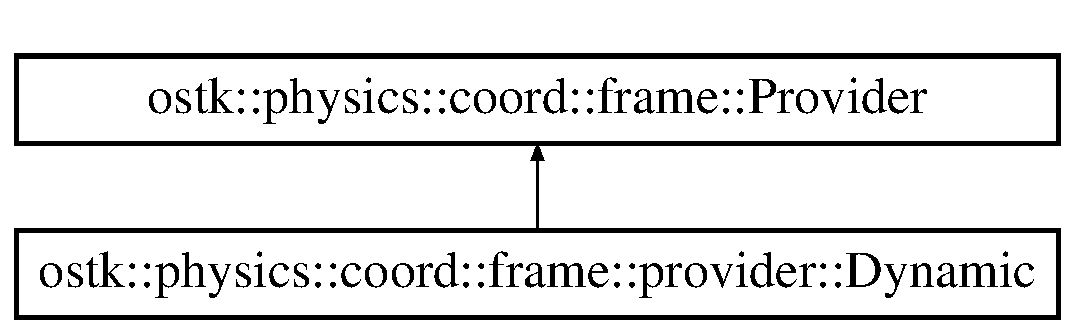
\includegraphics[height=2.000000cm]{classostk_1_1physics_1_1coord_1_1frame_1_1provider_1_1_dynamic}
\end{center}
\end{figure}
\subsection*{Public Types}
\begin{DoxyCompactItemize}
\item 
typedef std\+::function$<$ \hyperlink{classostk_1_1physics_1_1coord_1_1_transform}{Transform}(const \hyperlink{classostk_1_1physics_1_1time_1_1_instant}{Instant} \&)$>$ \hyperlink{classostk_1_1physics_1_1coord_1_1frame_1_1provider_1_1_dynamic_a1627a4b4e00ddcb81b50d3cabec711e8}{Generator}
\end{DoxyCompactItemize}
\subsection*{Public Member Functions}
\begin{DoxyCompactItemize}
\item 
\hyperlink{classostk_1_1physics_1_1coord_1_1frame_1_1provider_1_1_dynamic_a4a2d8961bc1ed12a2eafdf0c099a254f}{Dynamic} (const \hyperlink{classostk_1_1physics_1_1coord_1_1frame_1_1provider_1_1_dynamic_a1627a4b4e00ddcb81b50d3cabec711e8}{Dynamic\+::\+Generator} \&a\+Generator)
\item 
virtual \hyperlink{classostk_1_1physics_1_1coord_1_1frame_1_1provider_1_1_dynamic_a0f2a46aa108cfd9116c2e3ce00071597}{$\sim$\+Dynamic} () override
\item 
virtual \hyperlink{classostk_1_1physics_1_1coord_1_1frame_1_1provider_1_1_dynamic}{Dynamic} $\ast$ \hyperlink{classostk_1_1physics_1_1coord_1_1frame_1_1provider_1_1_dynamic_a37623142581671606ea45ca3bda0d0c8}{clone} () const override
\item 
virtual bool \hyperlink{classostk_1_1physics_1_1coord_1_1frame_1_1provider_1_1_dynamic_ab01d8d9a09df8e46680eb1acb830a86c}{is\+Defined} () const override
\item 
virtual \hyperlink{classostk_1_1physics_1_1coord_1_1_transform}{Transform} \hyperlink{classostk_1_1physics_1_1coord_1_1frame_1_1provider_1_1_dynamic_a7b7bfc8957fd84d90d0479944a427005}{get\+Transform\+At} (const \hyperlink{classostk_1_1physics_1_1time_1_1_instant}{Instant} \&an\+Instant) const override
\end{DoxyCompactItemize}
\subsection*{Static Public Member Functions}
\begin{DoxyCompactItemize}
\item 
static \hyperlink{classostk_1_1physics_1_1coord_1_1frame_1_1provider_1_1_dynamic}{Dynamic} \hyperlink{classostk_1_1physics_1_1coord_1_1frame_1_1provider_1_1_dynamic_aee37346f8f67c537c87c490ecf48238c}{Undefined} ()
\end{DoxyCompactItemize}


\subsection{Detailed Description}
\hyperlink{classostk_1_1physics_1_1coord_1_1frame_1_1provider_1_1_dynamic}{Dynamic} provider. 

\subsection{Member Typedef Documentation}
\mbox{\Hypertarget{classostk_1_1physics_1_1coord_1_1frame_1_1provider_1_1_dynamic_a1627a4b4e00ddcb81b50d3cabec711e8}\label{classostk_1_1physics_1_1coord_1_1frame_1_1provider_1_1_dynamic_a1627a4b4e00ddcb81b50d3cabec711e8}} 
\index{ostk\+::physics\+::coord\+::frame\+::provider\+::\+Dynamic@{ostk\+::physics\+::coord\+::frame\+::provider\+::\+Dynamic}!Generator@{Generator}}
\index{Generator@{Generator}!ostk\+::physics\+::coord\+::frame\+::provider\+::\+Dynamic@{ostk\+::physics\+::coord\+::frame\+::provider\+::\+Dynamic}}
\subsubsection{\texorpdfstring{Generator}{Generator}}
{\footnotesize\ttfamily typedef std\+::function$<$\hyperlink{classostk_1_1physics_1_1coord_1_1_transform}{Transform} (const \hyperlink{classostk_1_1physics_1_1time_1_1_instant}{Instant}\&)$>$ \hyperlink{classostk_1_1physics_1_1coord_1_1frame_1_1provider_1_1_dynamic_a1627a4b4e00ddcb81b50d3cabec711e8}{ostk\+::physics\+::coord\+::frame\+::provider\+::\+Dynamic\+::\+Generator}}



\subsection{Constructor \& Destructor Documentation}
\mbox{\Hypertarget{classostk_1_1physics_1_1coord_1_1frame_1_1provider_1_1_dynamic_a4a2d8961bc1ed12a2eafdf0c099a254f}\label{classostk_1_1physics_1_1coord_1_1frame_1_1provider_1_1_dynamic_a4a2d8961bc1ed12a2eafdf0c099a254f}} 
\index{ostk\+::physics\+::coord\+::frame\+::provider\+::\+Dynamic@{ostk\+::physics\+::coord\+::frame\+::provider\+::\+Dynamic}!Dynamic@{Dynamic}}
\index{Dynamic@{Dynamic}!ostk\+::physics\+::coord\+::frame\+::provider\+::\+Dynamic@{ostk\+::physics\+::coord\+::frame\+::provider\+::\+Dynamic}}
\subsubsection{\texorpdfstring{Dynamic()}{Dynamic()}}
{\footnotesize\ttfamily ostk\+::physics\+::coord\+::frame\+::provider\+::\+Dynamic\+::\+Dynamic (\begin{DoxyParamCaption}\item[{const \hyperlink{classostk_1_1physics_1_1coord_1_1frame_1_1provider_1_1_dynamic_a1627a4b4e00ddcb81b50d3cabec711e8}{Dynamic\+::\+Generator} \&}]{a\+Generator }\end{DoxyParamCaption})}

\mbox{\Hypertarget{classostk_1_1physics_1_1coord_1_1frame_1_1provider_1_1_dynamic_a0f2a46aa108cfd9116c2e3ce00071597}\label{classostk_1_1physics_1_1coord_1_1frame_1_1provider_1_1_dynamic_a0f2a46aa108cfd9116c2e3ce00071597}} 
\index{ostk\+::physics\+::coord\+::frame\+::provider\+::\+Dynamic@{ostk\+::physics\+::coord\+::frame\+::provider\+::\+Dynamic}!````~Dynamic@{$\sim$\+Dynamic}}
\index{````~Dynamic@{$\sim$\+Dynamic}!ostk\+::physics\+::coord\+::frame\+::provider\+::\+Dynamic@{ostk\+::physics\+::coord\+::frame\+::provider\+::\+Dynamic}}
\subsubsection{\texorpdfstring{$\sim$\+Dynamic()}{~Dynamic()}}
{\footnotesize\ttfamily ostk\+::physics\+::coord\+::frame\+::provider\+::\+Dynamic\+::$\sim$\+Dynamic (\begin{DoxyParamCaption}{ }\end{DoxyParamCaption})\hspace{0.3cm}{\ttfamily [override]}, {\ttfamily [virtual]}}



\subsection{Member Function Documentation}
\mbox{\Hypertarget{classostk_1_1physics_1_1coord_1_1frame_1_1provider_1_1_dynamic_a37623142581671606ea45ca3bda0d0c8}\label{classostk_1_1physics_1_1coord_1_1frame_1_1provider_1_1_dynamic_a37623142581671606ea45ca3bda0d0c8}} 
\index{ostk\+::physics\+::coord\+::frame\+::provider\+::\+Dynamic@{ostk\+::physics\+::coord\+::frame\+::provider\+::\+Dynamic}!clone@{clone}}
\index{clone@{clone}!ostk\+::physics\+::coord\+::frame\+::provider\+::\+Dynamic@{ostk\+::physics\+::coord\+::frame\+::provider\+::\+Dynamic}}
\subsubsection{\texorpdfstring{clone()}{clone()}}
{\footnotesize\ttfamily \hyperlink{classostk_1_1physics_1_1coord_1_1frame_1_1provider_1_1_dynamic}{Dynamic} $\ast$ ostk\+::physics\+::coord\+::frame\+::provider\+::\+Dynamic\+::clone (\begin{DoxyParamCaption}{ }\end{DoxyParamCaption}) const\hspace{0.3cm}{\ttfamily [override]}, {\ttfamily [virtual]}}



Implements \hyperlink{classostk_1_1physics_1_1coord_1_1frame_1_1_provider_ae41bc3862d088e9c8d90a79253294ce9}{ostk\+::physics\+::coord\+::frame\+::\+Provider}.

\mbox{\Hypertarget{classostk_1_1physics_1_1coord_1_1frame_1_1provider_1_1_dynamic_a7b7bfc8957fd84d90d0479944a427005}\label{classostk_1_1physics_1_1coord_1_1frame_1_1provider_1_1_dynamic_a7b7bfc8957fd84d90d0479944a427005}} 
\index{ostk\+::physics\+::coord\+::frame\+::provider\+::\+Dynamic@{ostk\+::physics\+::coord\+::frame\+::provider\+::\+Dynamic}!get\+Transform\+At@{get\+Transform\+At}}
\index{get\+Transform\+At@{get\+Transform\+At}!ostk\+::physics\+::coord\+::frame\+::provider\+::\+Dynamic@{ostk\+::physics\+::coord\+::frame\+::provider\+::\+Dynamic}}
\subsubsection{\texorpdfstring{get\+Transform\+At()}{getTransformAt()}}
{\footnotesize\ttfamily \hyperlink{classostk_1_1physics_1_1coord_1_1_transform}{Transform} ostk\+::physics\+::coord\+::frame\+::provider\+::\+Dynamic\+::get\+Transform\+At (\begin{DoxyParamCaption}\item[{const \hyperlink{classostk_1_1physics_1_1time_1_1_instant}{Instant} \&}]{an\+Instant }\end{DoxyParamCaption}) const\hspace{0.3cm}{\ttfamily [override]}, {\ttfamily [virtual]}}



Implements \hyperlink{classostk_1_1physics_1_1coord_1_1frame_1_1_provider_a38b86a589f46f8b8a9c97ab2776f37d1}{ostk\+::physics\+::coord\+::frame\+::\+Provider}.

\mbox{\Hypertarget{classostk_1_1physics_1_1coord_1_1frame_1_1provider_1_1_dynamic_ab01d8d9a09df8e46680eb1acb830a86c}\label{classostk_1_1physics_1_1coord_1_1frame_1_1provider_1_1_dynamic_ab01d8d9a09df8e46680eb1acb830a86c}} 
\index{ostk\+::physics\+::coord\+::frame\+::provider\+::\+Dynamic@{ostk\+::physics\+::coord\+::frame\+::provider\+::\+Dynamic}!is\+Defined@{is\+Defined}}
\index{is\+Defined@{is\+Defined}!ostk\+::physics\+::coord\+::frame\+::provider\+::\+Dynamic@{ostk\+::physics\+::coord\+::frame\+::provider\+::\+Dynamic}}
\subsubsection{\texorpdfstring{is\+Defined()}{isDefined()}}
{\footnotesize\ttfamily bool ostk\+::physics\+::coord\+::frame\+::provider\+::\+Dynamic\+::is\+Defined (\begin{DoxyParamCaption}{ }\end{DoxyParamCaption}) const\hspace{0.3cm}{\ttfamily [override]}, {\ttfamily [virtual]}}



Implements \hyperlink{classostk_1_1physics_1_1coord_1_1frame_1_1_provider_a27acab0012649796b97956fed1a91493}{ostk\+::physics\+::coord\+::frame\+::\+Provider}.

\mbox{\Hypertarget{classostk_1_1physics_1_1coord_1_1frame_1_1provider_1_1_dynamic_aee37346f8f67c537c87c490ecf48238c}\label{classostk_1_1physics_1_1coord_1_1frame_1_1provider_1_1_dynamic_aee37346f8f67c537c87c490ecf48238c}} 
\index{ostk\+::physics\+::coord\+::frame\+::provider\+::\+Dynamic@{ostk\+::physics\+::coord\+::frame\+::provider\+::\+Dynamic}!Undefined@{Undefined}}
\index{Undefined@{Undefined}!ostk\+::physics\+::coord\+::frame\+::provider\+::\+Dynamic@{ostk\+::physics\+::coord\+::frame\+::provider\+::\+Dynamic}}
\subsubsection{\texorpdfstring{Undefined()}{Undefined()}}
{\footnotesize\ttfamily \hyperlink{classostk_1_1physics_1_1coord_1_1frame_1_1provider_1_1_dynamic}{Dynamic} ostk\+::physics\+::coord\+::frame\+::provider\+::\+Dynamic\+::\+Undefined (\begin{DoxyParamCaption}{ }\end{DoxyParamCaption})\hspace{0.3cm}{\ttfamily [static]}}



The documentation for this class was generated from the following files\+:\begin{DoxyCompactItemize}
\item 
include/\+Open\+Space\+Toolkit/\+Physics/\+Coordinate/\+Frame/\+Providers/\hyperlink{_dynamic_8hpp}{Dynamic.\+hpp}\item 
src/\+Open\+Space\+Toolkit/\+Physics/\+Coordinate/\+Frame/\+Providers/\hyperlink{_dynamic_8cpp}{Dynamic.\+cpp}\end{DoxyCompactItemize}

\hypertarget{classostk_1_1physics_1_1environment_1_1gravitational_1_1_earth}{}\section{ostk\+:\+:physics\+:\+:environment\+:\+:gravitational\+:\+:Earth Class Reference}
\label{classostk_1_1physics_1_1environment_1_1gravitational_1_1_earth}\index{ostk\+::physics\+::environment\+::gravitational\+::\+Earth@{ostk\+::physics\+::environment\+::gravitational\+::\+Earth}}


\hyperlink{classostk_1_1physics_1_1environment_1_1gravitational_1_1_earth}{Earth} gravitational model.  




{\ttfamily \#include $<$Earth.\+hpp$>$}

Inheritance diagram for ostk\+:\+:physics\+:\+:environment\+:\+:gravitational\+:\+:Earth\+:\begin{figure}[H]
\begin{center}
\leavevmode
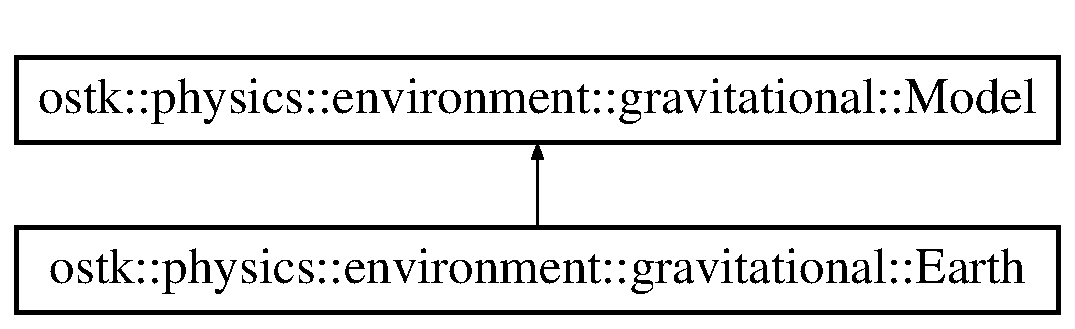
\includegraphics[height=2.000000cm]{classostk_1_1physics_1_1environment_1_1gravitational_1_1_earth}
\end{center}
\end{figure}
\subsection*{Public Types}
\begin{DoxyCompactItemize}
\item 
enum \hyperlink{classostk_1_1physics_1_1environment_1_1gravitational_1_1_earth_a9895df78b5c5aab5e981bf765f8c0f05}{Type} \{ \hyperlink{classostk_1_1physics_1_1environment_1_1gravitational_1_1_earth_a9895df78b5c5aab5e981bf765f8c0f05a5dda43a21474cf33e7088b8247f19c4b}{Type\+::\+W\+G\+S84}, 
\hyperlink{classostk_1_1physics_1_1environment_1_1gravitational_1_1_earth_a9895df78b5c5aab5e981bf765f8c0f05a2ae5659e79a4bb66ae4ee8cb033ef196}{Type\+::\+E\+G\+M84}, 
\hyperlink{classostk_1_1physics_1_1environment_1_1gravitational_1_1_earth_a9895df78b5c5aab5e981bf765f8c0f05a7c7ad846cb98dafc9309087d3ba36013}{Type\+::\+E\+G\+M96}, 
\hyperlink{classostk_1_1physics_1_1environment_1_1gravitational_1_1_earth_a9895df78b5c5aab5e981bf765f8c0f05af22fbbe07f6feeaa3d6446dabcd8b164}{Type\+::\+E\+G\+M2008}
 \}
\end{DoxyCompactItemize}
\subsection*{Public Member Functions}
\begin{DoxyCompactItemize}
\item 
\hyperlink{classostk_1_1physics_1_1environment_1_1gravitational_1_1_earth_a2266b9103f680d49643a5a8b4739a323}{Earth} (const \hyperlink{classostk_1_1physics_1_1environment_1_1gravitational_1_1_earth_a9895df78b5c5aab5e981bf765f8c0f05}{Earth\+::\+Type} \&a\+Type, const Directory \&a\+Data\+Directory=Directory\+::\+Undefined())
\begin{DoxyCompactList}\small\item\em Constructor. \end{DoxyCompactList}\item 
\hyperlink{classostk_1_1physics_1_1environment_1_1gravitational_1_1_earth_a821f98411c65f59e6a297c6bcc3de291}{Earth} (const \hyperlink{classostk_1_1physics_1_1environment_1_1gravitational_1_1_earth}{Earth} \&an\+Earth\+Gravitational\+Model)
\begin{DoxyCompactList}\small\item\em Copy constructor. \end{DoxyCompactList}\item 
\hyperlink{classostk_1_1physics_1_1environment_1_1gravitational_1_1_earth}{Earth} \& \hyperlink{classostk_1_1physics_1_1environment_1_1gravitational_1_1_earth_accc913e0c0a5c7c8348c13217c5de4f3}{operator=} (const \hyperlink{classostk_1_1physics_1_1environment_1_1gravitational_1_1_earth}{Earth} \&an\+Earth\+Gravitational\+Model)
\begin{DoxyCompactList}\small\item\em Copy assignment operator. \end{DoxyCompactList}\item 
\hyperlink{classostk_1_1physics_1_1environment_1_1gravitational_1_1_earth_a0bd1037605f6fb37fb6babc7bb8ae745}{$\sim$\+Earth} ()
\begin{DoxyCompactList}\small\item\em Destructor. \end{DoxyCompactList}\item 
virtual \hyperlink{classostk_1_1physics_1_1environment_1_1gravitational_1_1_earth}{Earth} $\ast$ \hyperlink{classostk_1_1physics_1_1environment_1_1gravitational_1_1_earth_a987c2df62d8fedb368acf37e71ba7a47}{clone} () const override
\begin{DoxyCompactList}\small\item\em Clone the \hyperlink{classostk_1_1physics_1_1environment_1_1gravitational_1_1_earth}{Earth} gravitational model. \end{DoxyCompactList}\item 
\hyperlink{classostk_1_1physics_1_1environment_1_1gravitational_1_1_earth_a9895df78b5c5aab5e981bf765f8c0f05}{Earth\+::\+Type} \hyperlink{classostk_1_1physics_1_1environment_1_1gravitational_1_1_earth_aa65dd2a5ce980e8a4f7f502387c1ff61}{get\+Type} () const
\begin{DoxyCompactList}\small\item\em Get gravitational model type. \end{DoxyCompactList}\item 
virtual Vector3d \hyperlink{classostk_1_1physics_1_1environment_1_1gravitational_1_1_earth_a9e536649566761f4bdd467993abfcedd}{get\+Field\+Value\+At} (const Vector3d \&a\+Position, const \hyperlink{classostk_1_1physics_1_1time_1_1_instant}{Instant} \&an\+Instant) const override
\begin{DoxyCompactList}\small\item\em Get the gravitational field value at a given position and instant. \end{DoxyCompactList}\end{DoxyCompactItemize}


\subsection{Detailed Description}
\hyperlink{classostk_1_1physics_1_1environment_1_1gravitational_1_1_earth}{Earth} gravitational model. 

The gravitational potential is expanded as sum of spherical harmonics.

https\+://en.wikipedia.\+org/wiki/\+Spherical\+\_\+harmonics https\+://geographiclib.sourceforge.\+io/html/gravity.html 

\subsection{Member Enumeration Documentation}
\mbox{\Hypertarget{classostk_1_1physics_1_1environment_1_1gravitational_1_1_earth_a9895df78b5c5aab5e981bf765f8c0f05}\label{classostk_1_1physics_1_1environment_1_1gravitational_1_1_earth_a9895df78b5c5aab5e981bf765f8c0f05}} 
\index{ostk\+::physics\+::environment\+::gravitational\+::\+Earth@{ostk\+::physics\+::environment\+::gravitational\+::\+Earth}!Type@{Type}}
\index{Type@{Type}!ostk\+::physics\+::environment\+::gravitational\+::\+Earth@{ostk\+::physics\+::environment\+::gravitational\+::\+Earth}}
\subsubsection{\texorpdfstring{Type}{Type}}
{\footnotesize\ttfamily enum \hyperlink{classostk_1_1physics_1_1environment_1_1gravitational_1_1_earth_a9895df78b5c5aab5e981bf765f8c0f05}{ostk\+::physics\+::environment\+::gravitational\+::\+Earth\+::\+Type}\hspace{0.3cm}{\ttfamily [strong]}}

\begin{DoxyEnumFields}{Enumerator}
\raisebox{\heightof{T}}[0pt][0pt]{\index{W\+G\+S84@{W\+G\+S84}!ostk\+::physics\+::environment\+::gravitational\+::\+Earth@{ostk\+::physics\+::environment\+::gravitational\+::\+Earth}}\index{ostk\+::physics\+::environment\+::gravitational\+::\+Earth@{ostk\+::physics\+::environment\+::gravitational\+::\+Earth}!W\+G\+S84@{W\+G\+S84}}}\mbox{\Hypertarget{classostk_1_1physics_1_1environment_1_1gravitational_1_1_earth_a9895df78b5c5aab5e981bf765f8c0f05a5dda43a21474cf33e7088b8247f19c4b}\label{classostk_1_1physics_1_1environment_1_1gravitational_1_1_earth_a9895df78b5c5aab5e981bf765f8c0f05a5dda43a21474cf33e7088b8247f19c4b}} 
W\+G\+S84&The normal gravitational field for the reference ellipsoid. This includes the zonal coefficients up to order 20. \\
\hline

\raisebox{\heightof{T}}[0pt][0pt]{\index{E\+G\+M84@{E\+G\+M84}!ostk\+::physics\+::environment\+::gravitational\+::\+Earth@{ostk\+::physics\+::environment\+::gravitational\+::\+Earth}}\index{ostk\+::physics\+::environment\+::gravitational\+::\+Earth@{ostk\+::physics\+::environment\+::gravitational\+::\+Earth}!E\+G\+M84@{E\+G\+M84}}}\mbox{\Hypertarget{classostk_1_1physics_1_1environment_1_1gravitational_1_1_earth_a9895df78b5c5aab5e981bf765f8c0f05a2ae5659e79a4bb66ae4ee8cb033ef196}\label{classostk_1_1physics_1_1environment_1_1gravitational_1_1_earth_a9895df78b5c5aab5e981bf765f8c0f05a2ae5659e79a4bb66ae4ee8cb033ef196}} 
E\+G\+M84&The \hyperlink{classostk_1_1physics_1_1environment_1_1gravitational_1_1_earth}{Earth} Gravity \hyperlink{classostk_1_1physics_1_1environment_1_1gravitational_1_1_model}{Model} 1984, which includes terms up to degree 180. \\
\hline

\raisebox{\heightof{T}}[0pt][0pt]{\index{E\+G\+M96@{E\+G\+M96}!ostk\+::physics\+::environment\+::gravitational\+::\+Earth@{ostk\+::physics\+::environment\+::gravitational\+::\+Earth}}\index{ostk\+::physics\+::environment\+::gravitational\+::\+Earth@{ostk\+::physics\+::environment\+::gravitational\+::\+Earth}!E\+G\+M96@{E\+G\+M96}}}\mbox{\Hypertarget{classostk_1_1physics_1_1environment_1_1gravitational_1_1_earth_a9895df78b5c5aab5e981bf765f8c0f05a7c7ad846cb98dafc9309087d3ba36013}\label{classostk_1_1physics_1_1environment_1_1gravitational_1_1_earth_a9895df78b5c5aab5e981bf765f8c0f05a7c7ad846cb98dafc9309087d3ba36013}} 
E\+G\+M96&The \hyperlink{classostk_1_1physics_1_1environment_1_1gravitational_1_1_earth}{Earth} Gravity \hyperlink{classostk_1_1physics_1_1environment_1_1gravitational_1_1_model}{Model} 1996, which includes terms up to degree 360. \\
\hline

\raisebox{\heightof{T}}[0pt][0pt]{\index{E\+G\+M2008@{E\+G\+M2008}!ostk\+::physics\+::environment\+::gravitational\+::\+Earth@{ostk\+::physics\+::environment\+::gravitational\+::\+Earth}}\index{ostk\+::physics\+::environment\+::gravitational\+::\+Earth@{ostk\+::physics\+::environment\+::gravitational\+::\+Earth}!E\+G\+M2008@{E\+G\+M2008}}}\mbox{\Hypertarget{classostk_1_1physics_1_1environment_1_1gravitational_1_1_earth_a9895df78b5c5aab5e981bf765f8c0f05af22fbbe07f6feeaa3d6446dabcd8b164}\label{classostk_1_1physics_1_1environment_1_1gravitational_1_1_earth_a9895df78b5c5aab5e981bf765f8c0f05af22fbbe07f6feeaa3d6446dabcd8b164}} 
E\+G\+M2008&The \hyperlink{classostk_1_1physics_1_1environment_1_1gravitational_1_1_earth}{Earth} Gravity \hyperlink{classostk_1_1physics_1_1environment_1_1gravitational_1_1_model}{Model} 2008, which includes terms up to degree 2190. \\
\hline

\end{DoxyEnumFields}


\subsection{Constructor \& Destructor Documentation}
\mbox{\Hypertarget{classostk_1_1physics_1_1environment_1_1gravitational_1_1_earth_a2266b9103f680d49643a5a8b4739a323}\label{classostk_1_1physics_1_1environment_1_1gravitational_1_1_earth_a2266b9103f680d49643a5a8b4739a323}} 
\index{ostk\+::physics\+::environment\+::gravitational\+::\+Earth@{ostk\+::physics\+::environment\+::gravitational\+::\+Earth}!Earth@{Earth}}
\index{Earth@{Earth}!ostk\+::physics\+::environment\+::gravitational\+::\+Earth@{ostk\+::physics\+::environment\+::gravitational\+::\+Earth}}
\subsubsection{\texorpdfstring{Earth()}{Earth()}\hspace{0.1cm}{\footnotesize\ttfamily [1/2]}}
{\footnotesize\ttfamily ostk\+::physics\+::environment\+::gravitational\+::\+Earth\+::\+Earth (\begin{DoxyParamCaption}\item[{const \hyperlink{classostk_1_1physics_1_1environment_1_1gravitational_1_1_earth_a9895df78b5c5aab5e981bf765f8c0f05}{Earth\+::\+Type} \&}]{a\+Type,  }\item[{const Directory \&}]{a\+Data\+Directory = {\ttfamily Directory\+:\+:Undefined()} }\end{DoxyParamCaption})}



Constructor. 


\begin{DoxyParams}[1]{Parameters}
\mbox{\tt in}  & {\em a\+Type} & A gravitational model type \\
\hline
\mbox{\tt in}  & {\em (optional)} & a\+Data\+Directory A gravitational model data directory \\
\hline
\end{DoxyParams}
\mbox{\Hypertarget{classostk_1_1physics_1_1environment_1_1gravitational_1_1_earth_a821f98411c65f59e6a297c6bcc3de291}\label{classostk_1_1physics_1_1environment_1_1gravitational_1_1_earth_a821f98411c65f59e6a297c6bcc3de291}} 
\index{ostk\+::physics\+::environment\+::gravitational\+::\+Earth@{ostk\+::physics\+::environment\+::gravitational\+::\+Earth}!Earth@{Earth}}
\index{Earth@{Earth}!ostk\+::physics\+::environment\+::gravitational\+::\+Earth@{ostk\+::physics\+::environment\+::gravitational\+::\+Earth}}
\subsubsection{\texorpdfstring{Earth()}{Earth()}\hspace{0.1cm}{\footnotesize\ttfamily [2/2]}}
{\footnotesize\ttfamily ostk\+::physics\+::environment\+::gravitational\+::\+Earth\+::\+Earth (\begin{DoxyParamCaption}\item[{const \hyperlink{classostk_1_1physics_1_1environment_1_1gravitational_1_1_earth}{Earth} \&}]{an\+Earth\+Gravitational\+Model }\end{DoxyParamCaption})}



Copy constructor. 


\begin{DoxyParams}[1]{Parameters}
\mbox{\tt in}  & {\em an\+Earth\+Gravitational\+Model} & An \hyperlink{classostk_1_1physics_1_1environment_1_1gravitational_1_1_earth}{Earth} model \\
\hline
\end{DoxyParams}
\mbox{\Hypertarget{classostk_1_1physics_1_1environment_1_1gravitational_1_1_earth_a0bd1037605f6fb37fb6babc7bb8ae745}\label{classostk_1_1physics_1_1environment_1_1gravitational_1_1_earth_a0bd1037605f6fb37fb6babc7bb8ae745}} 
\index{ostk\+::physics\+::environment\+::gravitational\+::\+Earth@{ostk\+::physics\+::environment\+::gravitational\+::\+Earth}!````~Earth@{$\sim$\+Earth}}
\index{````~Earth@{$\sim$\+Earth}!ostk\+::physics\+::environment\+::gravitational\+::\+Earth@{ostk\+::physics\+::environment\+::gravitational\+::\+Earth}}
\subsubsection{\texorpdfstring{$\sim$\+Earth()}{~Earth()}}
{\footnotesize\ttfamily ostk\+::physics\+::environment\+::gravitational\+::\+Earth\+::$\sim$\+Earth (\begin{DoxyParamCaption}{ }\end{DoxyParamCaption})}



Destructor. 



\subsection{Member Function Documentation}
\mbox{\Hypertarget{classostk_1_1physics_1_1environment_1_1gravitational_1_1_earth_a987c2df62d8fedb368acf37e71ba7a47}\label{classostk_1_1physics_1_1environment_1_1gravitational_1_1_earth_a987c2df62d8fedb368acf37e71ba7a47}} 
\index{ostk\+::physics\+::environment\+::gravitational\+::\+Earth@{ostk\+::physics\+::environment\+::gravitational\+::\+Earth}!clone@{clone}}
\index{clone@{clone}!ostk\+::physics\+::environment\+::gravitational\+::\+Earth@{ostk\+::physics\+::environment\+::gravitational\+::\+Earth}}
\subsubsection{\texorpdfstring{clone()}{clone()}}
{\footnotesize\ttfamily \hyperlink{classostk_1_1physics_1_1environment_1_1gravitational_1_1_earth}{Earth} $\ast$ ostk\+::physics\+::environment\+::gravitational\+::\+Earth\+::clone (\begin{DoxyParamCaption}{ }\end{DoxyParamCaption}) const\hspace{0.3cm}{\ttfamily [override]}, {\ttfamily [virtual]}}



Clone the \hyperlink{classostk_1_1physics_1_1environment_1_1gravitational_1_1_earth}{Earth} gravitational model. 

\begin{DoxyReturn}{Returns}
Pointer to \hyperlink{classostk_1_1physics_1_1environment_1_1gravitational_1_1_earth}{Earth} gravitational model 
\end{DoxyReturn}


Implements \hyperlink{classostk_1_1physics_1_1environment_1_1gravitational_1_1_model_a399257ac86e7f0112a702141e0e2e4a7}{ostk\+::physics\+::environment\+::gravitational\+::\+Model}.

\mbox{\Hypertarget{classostk_1_1physics_1_1environment_1_1gravitational_1_1_earth_a9e536649566761f4bdd467993abfcedd}\label{classostk_1_1physics_1_1environment_1_1gravitational_1_1_earth_a9e536649566761f4bdd467993abfcedd}} 
\index{ostk\+::physics\+::environment\+::gravitational\+::\+Earth@{ostk\+::physics\+::environment\+::gravitational\+::\+Earth}!get\+Field\+Value\+At@{get\+Field\+Value\+At}}
\index{get\+Field\+Value\+At@{get\+Field\+Value\+At}!ostk\+::physics\+::environment\+::gravitational\+::\+Earth@{ostk\+::physics\+::environment\+::gravitational\+::\+Earth}}
\subsubsection{\texorpdfstring{get\+Field\+Value\+At()}{getFieldValueAt()}}
{\footnotesize\ttfamily Vector3d ostk\+::physics\+::environment\+::gravitational\+::\+Earth\+::get\+Field\+Value\+At (\begin{DoxyParamCaption}\item[{const Vector3d \&}]{a\+Position,  }\item[{const \hyperlink{classostk_1_1physics_1_1time_1_1_instant}{Instant} \&}]{an\+Instant }\end{DoxyParamCaption}) const\hspace{0.3cm}{\ttfamily [override]}, {\ttfamily [virtual]}}



Get the gravitational field value at a given position and instant. 


\begin{DoxyParams}[1]{Parameters}
\mbox{\tt in}  & {\em a\+Position} & A position, expressed in the gravitational object frame \mbox{[}m\mbox{]} \\
\hline
\mbox{\tt in}  & {\em an\+Instant} & An instant \\
\hline
\end{DoxyParams}
\begin{DoxyReturn}{Returns}
Gravitational field value, expressed in the gravitational object frame \mbox{[}m.\+s-\/2\mbox{]} 
\end{DoxyReturn}


Implements \hyperlink{classostk_1_1physics_1_1environment_1_1gravitational_1_1_model_a5ef3b4ddf4240e8a26553294fe392581}{ostk\+::physics\+::environment\+::gravitational\+::\+Model}.

\mbox{\Hypertarget{classostk_1_1physics_1_1environment_1_1gravitational_1_1_earth_aa65dd2a5ce980e8a4f7f502387c1ff61}\label{classostk_1_1physics_1_1environment_1_1gravitational_1_1_earth_aa65dd2a5ce980e8a4f7f502387c1ff61}} 
\index{ostk\+::physics\+::environment\+::gravitational\+::\+Earth@{ostk\+::physics\+::environment\+::gravitational\+::\+Earth}!get\+Type@{get\+Type}}
\index{get\+Type@{get\+Type}!ostk\+::physics\+::environment\+::gravitational\+::\+Earth@{ostk\+::physics\+::environment\+::gravitational\+::\+Earth}}
\subsubsection{\texorpdfstring{get\+Type()}{getType()}}
{\footnotesize\ttfamily \hyperlink{classostk_1_1physics_1_1environment_1_1gravitational_1_1_earth_a9895df78b5c5aab5e981bf765f8c0f05}{Earth\+::\+Type} ostk\+::physics\+::environment\+::gravitational\+::\+Earth\+::get\+Type (\begin{DoxyParamCaption}{ }\end{DoxyParamCaption}) const}



Get gravitational model type. 

\begin{DoxyReturn}{Returns}
Gravitational model type 
\end{DoxyReturn}
\mbox{\Hypertarget{classostk_1_1physics_1_1environment_1_1gravitational_1_1_earth_accc913e0c0a5c7c8348c13217c5de4f3}\label{classostk_1_1physics_1_1environment_1_1gravitational_1_1_earth_accc913e0c0a5c7c8348c13217c5de4f3}} 
\index{ostk\+::physics\+::environment\+::gravitational\+::\+Earth@{ostk\+::physics\+::environment\+::gravitational\+::\+Earth}!operator=@{operator=}}
\index{operator=@{operator=}!ostk\+::physics\+::environment\+::gravitational\+::\+Earth@{ostk\+::physics\+::environment\+::gravitational\+::\+Earth}}
\subsubsection{\texorpdfstring{operator=()}{operator=()}}
{\footnotesize\ttfamily \hyperlink{classostk_1_1physics_1_1environment_1_1gravitational_1_1_earth}{Earth} \& ostk\+::physics\+::environment\+::gravitational\+::\+Earth\+::operator= (\begin{DoxyParamCaption}\item[{const \hyperlink{classostk_1_1physics_1_1environment_1_1gravitational_1_1_earth}{Earth} \&}]{an\+Earth\+Gravitational\+Model }\end{DoxyParamCaption})}



Copy assignment operator. 


\begin{DoxyParams}[1]{Parameters}
\mbox{\tt in}  & {\em an\+Earth\+Gravitational\+Model} & An \hyperlink{classostk_1_1physics_1_1environment_1_1gravitational_1_1_earth}{Earth} model \\
\hline
\end{DoxyParams}
\begin{DoxyReturn}{Returns}
Reference to \hyperlink{classostk_1_1physics_1_1environment_1_1gravitational_1_1_earth}{Earth} model 
\end{DoxyReturn}


The documentation for this class was generated from the following files\+:\begin{DoxyCompactItemize}
\item 
include/\+Open\+Space\+Toolkit/\+Physics/\+Environment/\+Gravitational/\hyperlink{_gravitational_2_earth_8hpp}{Earth.\+hpp}\item 
src/\+Open\+Space\+Toolkit/\+Physics/\+Environment/\+Gravitational/\hyperlink{_gravitational_2_earth_8cpp}{Earth.\+cpp}\end{DoxyCompactItemize}

\hypertarget{classostk_1_1physics_1_1environment_1_1magnetic_1_1_earth}{}\section{ostk\+:\+:physics\+:\+:environment\+:\+:magnetic\+:\+:Earth Class Reference}
\label{classostk_1_1physics_1_1environment_1_1magnetic_1_1_earth}\index{ostk\+::physics\+::environment\+::magnetic\+::\+Earth@{ostk\+::physics\+::environment\+::magnetic\+::\+Earth}}


\hyperlink{classostk_1_1physics_1_1environment_1_1magnetic_1_1_earth}{Earth} magnetic model.  




{\ttfamily \#include $<$Earth.\+hpp$>$}

Inheritance diagram for ostk\+:\+:physics\+:\+:environment\+:\+:magnetic\+:\+:Earth\+:\begin{figure}[H]
\begin{center}
\leavevmode
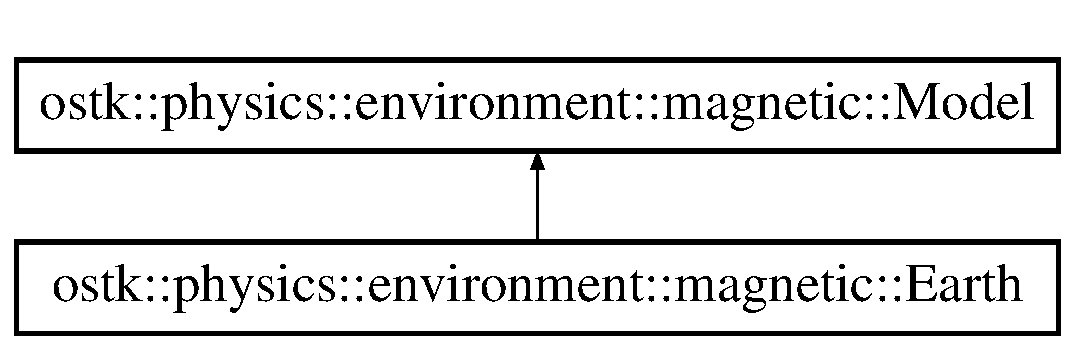
\includegraphics[height=2.000000cm]{classostk_1_1physics_1_1environment_1_1magnetic_1_1_earth}
\end{center}
\end{figure}
\subsection*{Public Types}
\begin{DoxyCompactItemize}
\item 
enum \hyperlink{classostk_1_1physics_1_1environment_1_1magnetic_1_1_earth_a30a064d87b6fce338e76aebd3043b6b6}{Type} \{ \newline
\hyperlink{classostk_1_1physics_1_1environment_1_1magnetic_1_1_earth_a30a064d87b6fce338e76aebd3043b6b6a7627ce84eadbc3098e818fa89b368c2c}{Type\+::\+Dipole}, 
\hyperlink{classostk_1_1physics_1_1environment_1_1magnetic_1_1_earth_a30a064d87b6fce338e76aebd3043b6b6aed2fcd927feb1858e659c2278acc9b04}{Type\+::\+E\+M\+M2010}, 
\hyperlink{classostk_1_1physics_1_1environment_1_1magnetic_1_1_earth_a30a064d87b6fce338e76aebd3043b6b6abeb005aa2afa040561e58b462da8583d}{Type\+::\+E\+M\+M2015}, 
\hyperlink{classostk_1_1physics_1_1environment_1_1magnetic_1_1_earth_a30a064d87b6fce338e76aebd3043b6b6a19d30648df1be691437893aae34fcf62}{Type\+::\+E\+M\+M2017}, 
\newline
\hyperlink{classostk_1_1physics_1_1environment_1_1magnetic_1_1_earth_a30a064d87b6fce338e76aebd3043b6b6aa2ad57512dc0d08c7e8937152ebec747}{Type\+::\+I\+G\+R\+F11}, 
\hyperlink{classostk_1_1physics_1_1environment_1_1magnetic_1_1_earth_a30a064d87b6fce338e76aebd3043b6b6a9a61c68f57fc5ed7927cfcec00291c11}{Type\+::\+I\+G\+R\+F12}, 
\hyperlink{classostk_1_1physics_1_1environment_1_1magnetic_1_1_earth_a30a064d87b6fce338e76aebd3043b6b6acf25da7a5a5ba3ab08e4c26071ed0b20}{Type\+::\+W\+M\+M2010}, 
\hyperlink{classostk_1_1physics_1_1environment_1_1magnetic_1_1_earth_a30a064d87b6fce338e76aebd3043b6b6a164a99cca8995f690571ed8f964e6166}{Type\+::\+W\+M\+M2015}
 \}
\end{DoxyCompactItemize}
\subsection*{Public Member Functions}
\begin{DoxyCompactItemize}
\item 
\hyperlink{classostk_1_1physics_1_1environment_1_1magnetic_1_1_earth_ade6f1fc6f3a69543e2bb1921aa8168c5}{Earth} (const \hyperlink{classostk_1_1physics_1_1environment_1_1magnetic_1_1_earth_a30a064d87b6fce338e76aebd3043b6b6}{Earth\+::\+Type} \&a\+Type, const Directory \&a\+Data\+Directory=Directory\+::\+Undefined())
\begin{DoxyCompactList}\small\item\em Constructor. \end{DoxyCompactList}\item 
\hyperlink{classostk_1_1physics_1_1environment_1_1magnetic_1_1_earth_a0d12c37ce2e12e778a01d5c79dcfd355}{Earth} (const \hyperlink{classostk_1_1physics_1_1environment_1_1magnetic_1_1_earth}{Earth} \&an\+Earth\+Magnetic\+Model)
\begin{DoxyCompactList}\small\item\em Copy constructor. \end{DoxyCompactList}\item 
\hyperlink{classostk_1_1physics_1_1environment_1_1magnetic_1_1_earth}{Earth} \& \hyperlink{classostk_1_1physics_1_1environment_1_1magnetic_1_1_earth_ad7ce781762b59980fb255b3b2a3f6aca}{operator=} (const \hyperlink{classostk_1_1physics_1_1environment_1_1magnetic_1_1_earth}{Earth} \&an\+Earth\+Magnetic\+Model)
\begin{DoxyCompactList}\small\item\em Copy assignment operator. \end{DoxyCompactList}\item 
\hyperlink{classostk_1_1physics_1_1environment_1_1magnetic_1_1_earth_a980e325b00a1dc56103d18c3199d0e33}{$\sim$\+Earth} ()
\begin{DoxyCompactList}\small\item\em Destructor. \end{DoxyCompactList}\item 
virtual \hyperlink{classostk_1_1physics_1_1environment_1_1magnetic_1_1_earth}{Earth} $\ast$ \hyperlink{classostk_1_1physics_1_1environment_1_1magnetic_1_1_earth_ac4b57f94304595595fc3eebb0dd0d050}{clone} () const override
\begin{DoxyCompactList}\small\item\em Clone the \hyperlink{classostk_1_1physics_1_1environment_1_1magnetic_1_1_earth}{Earth} magnetic model. \end{DoxyCompactList}\item 
\hyperlink{classostk_1_1physics_1_1environment_1_1magnetic_1_1_earth_a30a064d87b6fce338e76aebd3043b6b6}{Earth\+::\+Type} \hyperlink{classostk_1_1physics_1_1environment_1_1magnetic_1_1_earth_a20952c06c726e4f89f2f8184653ea74e}{get\+Type} () const
\begin{DoxyCompactList}\small\item\em Get magnetic model type. \end{DoxyCompactList}\item 
virtual Vector3d \hyperlink{classostk_1_1physics_1_1environment_1_1magnetic_1_1_earth_a2f39ff75c4a674b6720b27c2c6a0b930}{get\+Field\+Value\+At} (const Vector3d \&a\+Position, const \hyperlink{classostk_1_1physics_1_1time_1_1_instant}{Instant} \&an\+Instant) const override
\begin{DoxyCompactList}\small\item\em Get the magnetic field value at a given position and instant. \end{DoxyCompactList}\end{DoxyCompactItemize}


\subsection{Detailed Description}
\hyperlink{classostk_1_1physics_1_1environment_1_1magnetic_1_1_earth}{Earth} magnetic model. 

https\+://geographiclib.sourceforge.\+io/html/magnetic.html 

\subsection{Member Enumeration Documentation}
\mbox{\Hypertarget{classostk_1_1physics_1_1environment_1_1magnetic_1_1_earth_a30a064d87b6fce338e76aebd3043b6b6}\label{classostk_1_1physics_1_1environment_1_1magnetic_1_1_earth_a30a064d87b6fce338e76aebd3043b6b6}} 
\index{ostk\+::physics\+::environment\+::magnetic\+::\+Earth@{ostk\+::physics\+::environment\+::magnetic\+::\+Earth}!Type@{Type}}
\index{Type@{Type}!ostk\+::physics\+::environment\+::magnetic\+::\+Earth@{ostk\+::physics\+::environment\+::magnetic\+::\+Earth}}
\subsubsection{\texorpdfstring{Type}{Type}}
{\footnotesize\ttfamily enum \hyperlink{classostk_1_1physics_1_1environment_1_1magnetic_1_1_earth_a30a064d87b6fce338e76aebd3043b6b6}{ostk\+::physics\+::environment\+::magnetic\+::\+Earth\+::\+Type}\hspace{0.3cm}{\ttfamily [strong]}}

\begin{DoxyEnumFields}{Enumerator}
\raisebox{\heightof{T}}[0pt][0pt]{\index{Dipole@{Dipole}!ostk\+::physics\+::environment\+::magnetic\+::\+Earth@{ostk\+::physics\+::environment\+::magnetic\+::\+Earth}}\index{ostk\+::physics\+::environment\+::magnetic\+::\+Earth@{ostk\+::physics\+::environment\+::magnetic\+::\+Earth}!Dipole@{Dipole}}}\mbox{\Hypertarget{classostk_1_1physics_1_1environment_1_1magnetic_1_1_earth_a30a064d87b6fce338e76aebd3043b6b6a7627ce84eadbc3098e818fa89b368c2c}\label{classostk_1_1physics_1_1environment_1_1magnetic_1_1_earth_a30a064d87b6fce338e76aebd3043b6b6a7627ce84eadbc3098e818fa89b368c2c}} 
Dipole&\hyperlink{classostk_1_1physics_1_1environment_1_1magnetic_1_1_dipole}{Dipole} \hyperlink{classostk_1_1physics_1_1environment_1_1magnetic_1_1_model}{Model}. \\
\hline

\raisebox{\heightof{T}}[0pt][0pt]{\index{E\+M\+M2010@{E\+M\+M2010}!ostk\+::physics\+::environment\+::magnetic\+::\+Earth@{ostk\+::physics\+::environment\+::magnetic\+::\+Earth}}\index{ostk\+::physics\+::environment\+::magnetic\+::\+Earth@{ostk\+::physics\+::environment\+::magnetic\+::\+Earth}!E\+M\+M2010@{E\+M\+M2010}}}\mbox{\Hypertarget{classostk_1_1physics_1_1environment_1_1magnetic_1_1_earth_a30a064d87b6fce338e76aebd3043b6b6aed2fcd927feb1858e659c2278acc9b04}\label{classostk_1_1physics_1_1environment_1_1magnetic_1_1_earth_a30a064d87b6fce338e76aebd3043b6b6aed2fcd927feb1858e659c2278acc9b04}} 
E\+M\+M2010&Enhanced Magnetic \hyperlink{classostk_1_1physics_1_1environment_1_1magnetic_1_1_model}{Model} 2010\+: approximates the main and crustal magnetic fields for the period 2010–2015. \\
\hline

\raisebox{\heightof{T}}[0pt][0pt]{\index{E\+M\+M2015@{E\+M\+M2015}!ostk\+::physics\+::environment\+::magnetic\+::\+Earth@{ostk\+::physics\+::environment\+::magnetic\+::\+Earth}}\index{ostk\+::physics\+::environment\+::magnetic\+::\+Earth@{ostk\+::physics\+::environment\+::magnetic\+::\+Earth}!E\+M\+M2015@{E\+M\+M2015}}}\mbox{\Hypertarget{classostk_1_1physics_1_1environment_1_1magnetic_1_1_earth_a30a064d87b6fce338e76aebd3043b6b6abeb005aa2afa040561e58b462da8583d}\label{classostk_1_1physics_1_1environment_1_1magnetic_1_1_earth_a30a064d87b6fce338e76aebd3043b6b6abeb005aa2afa040561e58b462da8583d}} 
E\+M\+M2015&Enhanced Magnetic \hyperlink{classostk_1_1physics_1_1environment_1_1magnetic_1_1_model}{Model} 2015\+: approximates the main and crustal magnetic fields for the period 2000–2020. \\
\hline

\raisebox{\heightof{T}}[0pt][0pt]{\index{E\+M\+M2017@{E\+M\+M2017}!ostk\+::physics\+::environment\+::magnetic\+::\+Earth@{ostk\+::physics\+::environment\+::magnetic\+::\+Earth}}\index{ostk\+::physics\+::environment\+::magnetic\+::\+Earth@{ostk\+::physics\+::environment\+::magnetic\+::\+Earth}!E\+M\+M2017@{E\+M\+M2017}}}\mbox{\Hypertarget{classostk_1_1physics_1_1environment_1_1magnetic_1_1_earth_a30a064d87b6fce338e76aebd3043b6b6a19d30648df1be691437893aae34fcf62}\label{classostk_1_1physics_1_1environment_1_1magnetic_1_1_earth_a30a064d87b6fce338e76aebd3043b6b6a19d30648df1be691437893aae34fcf62}} 
E\+M\+M2017&Enhanced Magnetic \hyperlink{classostk_1_1physics_1_1environment_1_1magnetic_1_1_model}{Model} 2017\+: approximates the main and crustal magnetic fields for the period 2000–2022. \\
\hline

\raisebox{\heightof{T}}[0pt][0pt]{\index{I\+G\+R\+F11@{I\+G\+R\+F11}!ostk\+::physics\+::environment\+::magnetic\+::\+Earth@{ostk\+::physics\+::environment\+::magnetic\+::\+Earth}}\index{ostk\+::physics\+::environment\+::magnetic\+::\+Earth@{ostk\+::physics\+::environment\+::magnetic\+::\+Earth}!I\+G\+R\+F11@{I\+G\+R\+F11}}}\mbox{\Hypertarget{classostk_1_1physics_1_1environment_1_1magnetic_1_1_earth_a30a064d87b6fce338e76aebd3043b6b6aa2ad57512dc0d08c7e8937152ebec747}\label{classostk_1_1physics_1_1environment_1_1magnetic_1_1_earth_a30a064d87b6fce338e76aebd3043b6b6aa2ad57512dc0d08c7e8937152ebec747}} 
I\+G\+R\+F11&International Geomagnetic Reference Field (11th generation)\+: approximates the main magnetic field for the period 1900–2015. \\
\hline

\raisebox{\heightof{T}}[0pt][0pt]{\index{I\+G\+R\+F12@{I\+G\+R\+F12}!ostk\+::physics\+::environment\+::magnetic\+::\+Earth@{ostk\+::physics\+::environment\+::magnetic\+::\+Earth}}\index{ostk\+::physics\+::environment\+::magnetic\+::\+Earth@{ostk\+::physics\+::environment\+::magnetic\+::\+Earth}!I\+G\+R\+F12@{I\+G\+R\+F12}}}\mbox{\Hypertarget{classostk_1_1physics_1_1environment_1_1magnetic_1_1_earth_a30a064d87b6fce338e76aebd3043b6b6a9a61c68f57fc5ed7927cfcec00291c11}\label{classostk_1_1physics_1_1environment_1_1magnetic_1_1_earth_a30a064d87b6fce338e76aebd3043b6b6a9a61c68f57fc5ed7927cfcec00291c11}} 
I\+G\+R\+F12&International Geomagnetic Reference Field (12th generation)\+: approximates the main magnetic field for the period 1900–2020. \\
\hline

\raisebox{\heightof{T}}[0pt][0pt]{\index{W\+M\+M2010@{W\+M\+M2010}!ostk\+::physics\+::environment\+::magnetic\+::\+Earth@{ostk\+::physics\+::environment\+::magnetic\+::\+Earth}}\index{ostk\+::physics\+::environment\+::magnetic\+::\+Earth@{ostk\+::physics\+::environment\+::magnetic\+::\+Earth}!W\+M\+M2010@{W\+M\+M2010}}}\mbox{\Hypertarget{classostk_1_1physics_1_1environment_1_1magnetic_1_1_earth_a30a064d87b6fce338e76aebd3043b6b6acf25da7a5a5ba3ab08e4c26071ed0b20}\label{classostk_1_1physics_1_1environment_1_1magnetic_1_1_earth_a30a064d87b6fce338e76aebd3043b6b6acf25da7a5a5ba3ab08e4c26071ed0b20}} 
W\+M\+M2010&World Magnetic \hyperlink{classostk_1_1physics_1_1environment_1_1magnetic_1_1_model}{Model} 2010\+: approximates the main magnetic field for the period 2010–2015. \\
\hline

\raisebox{\heightof{T}}[0pt][0pt]{\index{W\+M\+M2015@{W\+M\+M2015}!ostk\+::physics\+::environment\+::magnetic\+::\+Earth@{ostk\+::physics\+::environment\+::magnetic\+::\+Earth}}\index{ostk\+::physics\+::environment\+::magnetic\+::\+Earth@{ostk\+::physics\+::environment\+::magnetic\+::\+Earth}!W\+M\+M2015@{W\+M\+M2015}}}\mbox{\Hypertarget{classostk_1_1physics_1_1environment_1_1magnetic_1_1_earth_a30a064d87b6fce338e76aebd3043b6b6a164a99cca8995f690571ed8f964e6166}\label{classostk_1_1physics_1_1environment_1_1magnetic_1_1_earth_a30a064d87b6fce338e76aebd3043b6b6a164a99cca8995f690571ed8f964e6166}} 
W\+M\+M2015&World Magnetic \hyperlink{classostk_1_1physics_1_1environment_1_1magnetic_1_1_model}{Model} 2015\+: approximates the main magnetic field for the period 2015–2020. \\
\hline

\end{DoxyEnumFields}


\subsection{Constructor \& Destructor Documentation}
\mbox{\Hypertarget{classostk_1_1physics_1_1environment_1_1magnetic_1_1_earth_ade6f1fc6f3a69543e2bb1921aa8168c5}\label{classostk_1_1physics_1_1environment_1_1magnetic_1_1_earth_ade6f1fc6f3a69543e2bb1921aa8168c5}} 
\index{ostk\+::physics\+::environment\+::magnetic\+::\+Earth@{ostk\+::physics\+::environment\+::magnetic\+::\+Earth}!Earth@{Earth}}
\index{Earth@{Earth}!ostk\+::physics\+::environment\+::magnetic\+::\+Earth@{ostk\+::physics\+::environment\+::magnetic\+::\+Earth}}
\subsubsection{\texorpdfstring{Earth()}{Earth()}\hspace{0.1cm}{\footnotesize\ttfamily [1/2]}}
{\footnotesize\ttfamily ostk\+::physics\+::environment\+::magnetic\+::\+Earth\+::\+Earth (\begin{DoxyParamCaption}\item[{const \hyperlink{classostk_1_1physics_1_1environment_1_1magnetic_1_1_earth_a30a064d87b6fce338e76aebd3043b6b6}{Earth\+::\+Type} \&}]{a\+Type,  }\item[{const Directory \&}]{a\+Data\+Directory = {\ttfamily Directory\+:\+:Undefined()} }\end{DoxyParamCaption})}



Constructor. 


\begin{DoxyParams}[1]{Parameters}
\mbox{\tt in}  & {\em a\+Type} & A magnetic model type \\
\hline
\mbox{\tt in}  & {\em (optional)} & a\+Data\+Directory A magnetic model data directory \\
\hline
\end{DoxyParams}
\mbox{\Hypertarget{classostk_1_1physics_1_1environment_1_1magnetic_1_1_earth_a0d12c37ce2e12e778a01d5c79dcfd355}\label{classostk_1_1physics_1_1environment_1_1magnetic_1_1_earth_a0d12c37ce2e12e778a01d5c79dcfd355}} 
\index{ostk\+::physics\+::environment\+::magnetic\+::\+Earth@{ostk\+::physics\+::environment\+::magnetic\+::\+Earth}!Earth@{Earth}}
\index{Earth@{Earth}!ostk\+::physics\+::environment\+::magnetic\+::\+Earth@{ostk\+::physics\+::environment\+::magnetic\+::\+Earth}}
\subsubsection{\texorpdfstring{Earth()}{Earth()}\hspace{0.1cm}{\footnotesize\ttfamily [2/2]}}
{\footnotesize\ttfamily ostk\+::physics\+::environment\+::magnetic\+::\+Earth\+::\+Earth (\begin{DoxyParamCaption}\item[{const \hyperlink{classostk_1_1physics_1_1environment_1_1magnetic_1_1_earth}{Earth} \&}]{an\+Earth\+Magnetic\+Model }\end{DoxyParamCaption})}



Copy constructor. 


\begin{DoxyParams}[1]{Parameters}
\mbox{\tt in}  & {\em an\+Earth\+Magnetic\+Model} & An \hyperlink{classostk_1_1physics_1_1environment_1_1magnetic_1_1_earth}{Earth} model \\
\hline
\end{DoxyParams}
\mbox{\Hypertarget{classostk_1_1physics_1_1environment_1_1magnetic_1_1_earth_a980e325b00a1dc56103d18c3199d0e33}\label{classostk_1_1physics_1_1environment_1_1magnetic_1_1_earth_a980e325b00a1dc56103d18c3199d0e33}} 
\index{ostk\+::physics\+::environment\+::magnetic\+::\+Earth@{ostk\+::physics\+::environment\+::magnetic\+::\+Earth}!````~Earth@{$\sim$\+Earth}}
\index{````~Earth@{$\sim$\+Earth}!ostk\+::physics\+::environment\+::magnetic\+::\+Earth@{ostk\+::physics\+::environment\+::magnetic\+::\+Earth}}
\subsubsection{\texorpdfstring{$\sim$\+Earth()}{~Earth()}}
{\footnotesize\ttfamily ostk\+::physics\+::environment\+::magnetic\+::\+Earth\+::$\sim$\+Earth (\begin{DoxyParamCaption}{ }\end{DoxyParamCaption})}



Destructor. 



\subsection{Member Function Documentation}
\mbox{\Hypertarget{classostk_1_1physics_1_1environment_1_1magnetic_1_1_earth_ac4b57f94304595595fc3eebb0dd0d050}\label{classostk_1_1physics_1_1environment_1_1magnetic_1_1_earth_ac4b57f94304595595fc3eebb0dd0d050}} 
\index{ostk\+::physics\+::environment\+::magnetic\+::\+Earth@{ostk\+::physics\+::environment\+::magnetic\+::\+Earth}!clone@{clone}}
\index{clone@{clone}!ostk\+::physics\+::environment\+::magnetic\+::\+Earth@{ostk\+::physics\+::environment\+::magnetic\+::\+Earth}}
\subsubsection{\texorpdfstring{clone()}{clone()}}
{\footnotesize\ttfamily \hyperlink{classostk_1_1physics_1_1environment_1_1magnetic_1_1_earth}{Earth} $\ast$ ostk\+::physics\+::environment\+::magnetic\+::\+Earth\+::clone (\begin{DoxyParamCaption}{ }\end{DoxyParamCaption}) const\hspace{0.3cm}{\ttfamily [override]}, {\ttfamily [virtual]}}



Clone the \hyperlink{classostk_1_1physics_1_1environment_1_1magnetic_1_1_earth}{Earth} magnetic model. 

\begin{DoxyReturn}{Returns}
Pointer to \hyperlink{classostk_1_1physics_1_1environment_1_1magnetic_1_1_earth}{Earth} magnetic model 
\end{DoxyReturn}


Implements \hyperlink{classostk_1_1physics_1_1environment_1_1magnetic_1_1_model_af357908c151a7809bbbc8fc676bd07b6}{ostk\+::physics\+::environment\+::magnetic\+::\+Model}.

\mbox{\Hypertarget{classostk_1_1physics_1_1environment_1_1magnetic_1_1_earth_a2f39ff75c4a674b6720b27c2c6a0b930}\label{classostk_1_1physics_1_1environment_1_1magnetic_1_1_earth_a2f39ff75c4a674b6720b27c2c6a0b930}} 
\index{ostk\+::physics\+::environment\+::magnetic\+::\+Earth@{ostk\+::physics\+::environment\+::magnetic\+::\+Earth}!get\+Field\+Value\+At@{get\+Field\+Value\+At}}
\index{get\+Field\+Value\+At@{get\+Field\+Value\+At}!ostk\+::physics\+::environment\+::magnetic\+::\+Earth@{ostk\+::physics\+::environment\+::magnetic\+::\+Earth}}
\subsubsection{\texorpdfstring{get\+Field\+Value\+At()}{getFieldValueAt()}}
{\footnotesize\ttfamily Vector3d ostk\+::physics\+::environment\+::magnetic\+::\+Earth\+::get\+Field\+Value\+At (\begin{DoxyParamCaption}\item[{const Vector3d \&}]{a\+Position,  }\item[{const \hyperlink{classostk_1_1physics_1_1time_1_1_instant}{Instant} \&}]{an\+Instant }\end{DoxyParamCaption}) const\hspace{0.3cm}{\ttfamily [override]}, {\ttfamily [virtual]}}



Get the magnetic field value at a given position and instant. 


\begin{DoxyParams}[1]{Parameters}
\mbox{\tt in}  & {\em a\+Position} & A position, expressed in the magnetic object frame \mbox{[}m\mbox{]} \\
\hline
\mbox{\tt in}  & {\em an\+Instant} & An instant \\
\hline
\end{DoxyParams}
\begin{DoxyReturn}{Returns}
Magnetic field value, expressed in the magnetic object frame \mbox{[}T\mbox{]} 
\end{DoxyReturn}


Implements \hyperlink{classostk_1_1physics_1_1environment_1_1magnetic_1_1_model_abf0510f9be2c196ea3c0586d02979b0f}{ostk\+::physics\+::environment\+::magnetic\+::\+Model}.

\mbox{\Hypertarget{classostk_1_1physics_1_1environment_1_1magnetic_1_1_earth_a20952c06c726e4f89f2f8184653ea74e}\label{classostk_1_1physics_1_1environment_1_1magnetic_1_1_earth_a20952c06c726e4f89f2f8184653ea74e}} 
\index{ostk\+::physics\+::environment\+::magnetic\+::\+Earth@{ostk\+::physics\+::environment\+::magnetic\+::\+Earth}!get\+Type@{get\+Type}}
\index{get\+Type@{get\+Type}!ostk\+::physics\+::environment\+::magnetic\+::\+Earth@{ostk\+::physics\+::environment\+::magnetic\+::\+Earth}}
\subsubsection{\texorpdfstring{get\+Type()}{getType()}}
{\footnotesize\ttfamily \hyperlink{classostk_1_1physics_1_1environment_1_1magnetic_1_1_earth_a30a064d87b6fce338e76aebd3043b6b6}{Earth\+::\+Type} ostk\+::physics\+::environment\+::magnetic\+::\+Earth\+::get\+Type (\begin{DoxyParamCaption}{ }\end{DoxyParamCaption}) const}



Get magnetic model type. 

\begin{DoxyReturn}{Returns}
Magnetic model type 
\end{DoxyReturn}
\mbox{\Hypertarget{classostk_1_1physics_1_1environment_1_1magnetic_1_1_earth_ad7ce781762b59980fb255b3b2a3f6aca}\label{classostk_1_1physics_1_1environment_1_1magnetic_1_1_earth_ad7ce781762b59980fb255b3b2a3f6aca}} 
\index{ostk\+::physics\+::environment\+::magnetic\+::\+Earth@{ostk\+::physics\+::environment\+::magnetic\+::\+Earth}!operator=@{operator=}}
\index{operator=@{operator=}!ostk\+::physics\+::environment\+::magnetic\+::\+Earth@{ostk\+::physics\+::environment\+::magnetic\+::\+Earth}}
\subsubsection{\texorpdfstring{operator=()}{operator=()}}
{\footnotesize\ttfamily \hyperlink{classostk_1_1physics_1_1environment_1_1magnetic_1_1_earth}{Earth} \& ostk\+::physics\+::environment\+::magnetic\+::\+Earth\+::operator= (\begin{DoxyParamCaption}\item[{const \hyperlink{classostk_1_1physics_1_1environment_1_1magnetic_1_1_earth}{Earth} \&}]{an\+Earth\+Magnetic\+Model }\end{DoxyParamCaption})}



Copy assignment operator. 


\begin{DoxyParams}[1]{Parameters}
\mbox{\tt in}  & {\em an\+Earth\+Magnetic\+Model} & An \hyperlink{classostk_1_1physics_1_1environment_1_1magnetic_1_1_earth}{Earth} model \\
\hline
\end{DoxyParams}
\begin{DoxyReturn}{Returns}
Reference to \hyperlink{classostk_1_1physics_1_1environment_1_1magnetic_1_1_earth}{Earth} model 
\end{DoxyReturn}


The documentation for this class was generated from the following files\+:\begin{DoxyCompactItemize}
\item 
include/\+Open\+Space\+Toolkit/\+Physics/\+Environment/\+Magnetic/\hyperlink{_magnetic_2_earth_8hpp}{Earth.\+hpp}\item 
src/\+Open\+Space\+Toolkit/\+Physics/\+Environment/\+Magnetic/\hyperlink{_magnetic_2_earth_8cpp}{Earth.\+cpp}\end{DoxyCompactItemize}

\hypertarget{classostk_1_1physics_1_1env_1_1obj_1_1celest_1_1_earth}{}\section{ostk\+:\+:physics\+:\+:env\+:\+:obj\+:\+:celest\+:\+:Earth Class Reference}
\label{classostk_1_1physics_1_1env_1_1obj_1_1celest_1_1_earth}\index{ostk\+::physics\+::env\+::obj\+::celest\+::\+Earth@{ostk\+::physics\+::env\+::obj\+::celest\+::\+Earth}}


{\ttfamily \#include $<$Earth.\+hpp$>$}

Inheritance diagram for ostk\+:\+:physics\+:\+:env\+:\+:obj\+:\+:celest\+:\+:Earth\+:\begin{figure}[H]
\begin{center}
\leavevmode
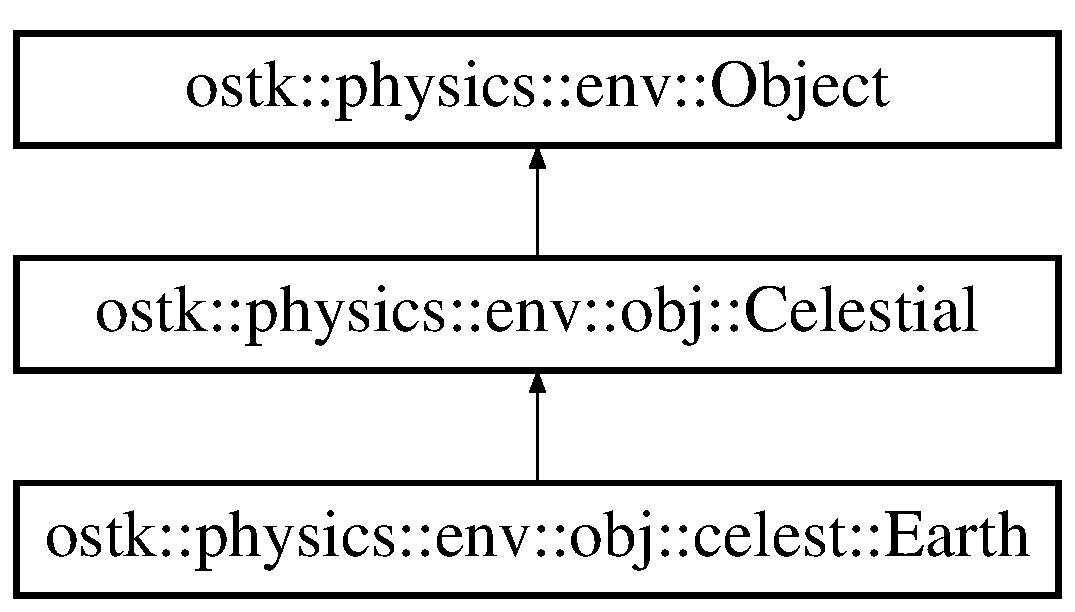
\includegraphics[height=3.000000cm]{classostk_1_1physics_1_1env_1_1obj_1_1celest_1_1_earth}
\end{center}
\end{figure}
\subsection*{Classes}
\begin{DoxyCompactItemize}
\item 
struct \hyperlink{structostk_1_1physics_1_1env_1_1obj_1_1celest_1_1_earth_1_1_models}{Models}
\end{DoxyCompactItemize}
\subsection*{Public Member Functions}
\begin{DoxyCompactItemize}
\item 
\hyperlink{classostk_1_1physics_1_1env_1_1obj_1_1celest_1_1_earth_aeed4d52f7da5b8f895701eb79826599a}{Earth} (const \hyperlink{classostk_1_1physics_1_1units_1_1_derived}{Derived} \&a\+Gravitational\+Parameter, const \hyperlink{classostk_1_1physics_1_1units_1_1_length}{Length} \&an\+Equatorial\+Radius, const Real \&a\+Flattening, const Real \&a\+J2, const Shared$<$ \hyperlink{classostk_1_1physics_1_1env_1_1_ephemeris}{Ephemeris} $>$ \&an\+Ephemeris, const \hyperlink{classostk_1_1physics_1_1environment_1_1gravitational_1_1_earth_a9895df78b5c5aab5e981bf765f8c0f05}{Earth\+Gravitational\+Model\+::\+Type} \&a\+Gravitational\+Model\+Type, const \hyperlink{classostk_1_1physics_1_1environment_1_1magnetic_1_1_earth_a30a064d87b6fce338e76aebd3043b6b6}{Earth\+Magnetic\+Model\+::\+Type} \&a\+Magnetic\+Model\+Type, const \hyperlink{classostk_1_1physics_1_1time_1_1_instant}{Instant} \&an\+Instant)
\item 
virtual \hyperlink{classostk_1_1physics_1_1env_1_1obj_1_1celest_1_1_earth_ac718f964c68fa41331978751a9ca4818}{$\sim$\+Earth} () override
\item 
virtual \hyperlink{classostk_1_1physics_1_1env_1_1obj_1_1celest_1_1_earth}{Earth} $\ast$ \hyperlink{classostk_1_1physics_1_1env_1_1obj_1_1celest_1_1_earth_ae86664b9d6fc870baa1dac5c3219f784}{clone} () const override
\end{DoxyCompactItemize}
\subsection*{Static Public Member Functions}
\begin{DoxyCompactItemize}
\item 
static \hyperlink{classostk_1_1physics_1_1env_1_1obj_1_1celest_1_1_earth}{Earth} \hyperlink{classostk_1_1physics_1_1env_1_1obj_1_1celest_1_1_earth_ab23224bee36577e7ab40576384ba8f2e}{Default} ()
\begin{DoxyCompactList}\small\item\em Default \hyperlink{classostk_1_1physics_1_1env_1_1obj_1_1celest_1_1_earth}{Earth} model (E\+G\+M2008) \end{DoxyCompactList}\item 
static \hyperlink{classostk_1_1physics_1_1env_1_1obj_1_1celest_1_1_earth}{Earth} \hyperlink{classostk_1_1physics_1_1env_1_1obj_1_1celest_1_1_earth_a69213489a7ce28c3dfa990283657b2bf}{E\+G\+M2008} ()
\begin{DoxyCompactList}\small\item\em \hyperlink{classostk_1_1physics_1_1env_1_1obj_1_1celest_1_1_earth}{Earth} Gravity Model 2008 model (E\+G\+M2008) \end{DoxyCompactList}\item 
static \hyperlink{classostk_1_1physics_1_1env_1_1obj_1_1celest_1_1_earth}{Earth} \hyperlink{classostk_1_1physics_1_1env_1_1obj_1_1celest_1_1_earth_a2c2af2af178d0eb24391a1ab19baa36a}{W\+G\+S84\+\_\+\+E\+G\+M96} ()
\begin{DoxyCompactList}\small\item\em World Geodetic System 1984 (W\+G\+S84) + \hyperlink{classostk_1_1physics_1_1env_1_1obj_1_1celest_1_1_earth}{Earth} Gravity Model 1996 (E\+G\+M96) \end{DoxyCompactList}\item 
static \hyperlink{classostk_1_1physics_1_1env_1_1obj_1_1celest_1_1_earth}{Earth} \hyperlink{classostk_1_1physics_1_1env_1_1obj_1_1celest_1_1_earth_ae86930600e872b2af40da227454fe49f}{E\+G\+M96} ()
\begin{DoxyCompactList}\small\item\em \hyperlink{classostk_1_1physics_1_1env_1_1obj_1_1celest_1_1_earth}{Earth} Gravity Model 1996 (E\+G\+M96) \end{DoxyCompactList}\item 
static \hyperlink{classostk_1_1physics_1_1env_1_1obj_1_1celest_1_1_earth}{Earth} \hyperlink{classostk_1_1physics_1_1env_1_1obj_1_1celest_1_1_earth_ad2c89b180e92bdc6c525ce7c065400aa}{W\+G\+S84} ()
\begin{DoxyCompactList}\small\item\em World Geodetic System 1984 (W\+G\+S84) \end{DoxyCompactList}\end{DoxyCompactItemize}
\subsection*{Static Public Attributes}
\begin{DoxyCompactItemize}
\item 
static const \hyperlink{classostk_1_1physics_1_1units_1_1_derived}{Derived} \hyperlink{classostk_1_1physics_1_1env_1_1obj_1_1celest_1_1_earth_a63bdb61b8a2b26066efc4ba7985c2060}{Gravitational\+Parameter} = Earth\+::\+Models\+::\+E\+G\+M2008\+::\+Gravitational\+Parameter
\item 
static const \hyperlink{classostk_1_1physics_1_1units_1_1_length}{Length} \hyperlink{classostk_1_1physics_1_1env_1_1obj_1_1celest_1_1_earth_ac700d34023a4654da6f781fc097034ad}{Equatorial\+Radius} = Earth\+::\+Models\+::\+E\+G\+M2008\+::\+Equatorial\+Radius
\item 
static const Real \hyperlink{classostk_1_1physics_1_1env_1_1obj_1_1celest_1_1_earth_ad1cb5b01fc6cdf263dd97aa5bcb62b78}{Flattening} = Earth\+::\+Models\+::\+E\+G\+M2008\+::\+Flattening
\item 
static const Real \hyperlink{classostk_1_1physics_1_1env_1_1obj_1_1celest_1_1_earth_a51d8f851ef1f2c199dbf7707d9843eb4}{C20} = Earth\+::\+Models\+::\+E\+G\+M2008\+::\+C20
\item 
static const Real \hyperlink{classostk_1_1physics_1_1env_1_1obj_1_1celest_1_1_earth_a0c09ef7a4fb1f6d5d077e4108fb4e56a}{J2} = Earth\+::\+Models\+::\+E\+G\+M2008\+::\+J2
\end{DoxyCompactItemize}
\subsection*{Additional Inherited Members}


\subsection{Constructor \& Destructor Documentation}
\mbox{\Hypertarget{classostk_1_1physics_1_1env_1_1obj_1_1celest_1_1_earth_aeed4d52f7da5b8f895701eb79826599a}\label{classostk_1_1physics_1_1env_1_1obj_1_1celest_1_1_earth_aeed4d52f7da5b8f895701eb79826599a}} 
\index{ostk\+::physics\+::env\+::obj\+::celest\+::\+Earth@{ostk\+::physics\+::env\+::obj\+::celest\+::\+Earth}!Earth@{Earth}}
\index{Earth@{Earth}!ostk\+::physics\+::env\+::obj\+::celest\+::\+Earth@{ostk\+::physics\+::env\+::obj\+::celest\+::\+Earth}}
\subsubsection{\texorpdfstring{Earth()}{Earth()}}
{\footnotesize\ttfamily ostk\+::physics\+::env\+::obj\+::celest\+::\+Earth\+::\+Earth (\begin{DoxyParamCaption}\item[{const \hyperlink{classostk_1_1physics_1_1units_1_1_derived}{Derived} \&}]{a\+Gravitational\+Parameter,  }\item[{const \hyperlink{classostk_1_1physics_1_1units_1_1_length}{Length} \&}]{an\+Equatorial\+Radius,  }\item[{const Real \&}]{a\+Flattening,  }\item[{const Real \&}]{a\+J2,  }\item[{const Shared$<$ \hyperlink{classostk_1_1physics_1_1env_1_1_ephemeris}{Ephemeris} $>$ \&}]{an\+Ephemeris,  }\item[{const \hyperlink{classostk_1_1physics_1_1environment_1_1gravitational_1_1_earth_a9895df78b5c5aab5e981bf765f8c0f05}{Earth\+Gravitational\+Model\+::\+Type} \&}]{a\+Gravitational\+Model\+Type,  }\item[{const \hyperlink{classostk_1_1physics_1_1environment_1_1magnetic_1_1_earth_a30a064d87b6fce338e76aebd3043b6b6}{Earth\+Magnetic\+Model\+::\+Type} \&}]{a\+Magnetic\+Model\+Type,  }\item[{const \hyperlink{classostk_1_1physics_1_1time_1_1_instant}{Instant} \&}]{an\+Instant }\end{DoxyParamCaption})}

\mbox{\Hypertarget{classostk_1_1physics_1_1env_1_1obj_1_1celest_1_1_earth_ac718f964c68fa41331978751a9ca4818}\label{classostk_1_1physics_1_1env_1_1obj_1_1celest_1_1_earth_ac718f964c68fa41331978751a9ca4818}} 
\index{ostk\+::physics\+::env\+::obj\+::celest\+::\+Earth@{ostk\+::physics\+::env\+::obj\+::celest\+::\+Earth}!````~Earth@{$\sim$\+Earth}}
\index{````~Earth@{$\sim$\+Earth}!ostk\+::physics\+::env\+::obj\+::celest\+::\+Earth@{ostk\+::physics\+::env\+::obj\+::celest\+::\+Earth}}
\subsubsection{\texorpdfstring{$\sim$\+Earth()}{~Earth()}}
{\footnotesize\ttfamily ostk\+::physics\+::env\+::obj\+::celest\+::\+Earth\+::$\sim$\+Earth (\begin{DoxyParamCaption}{ }\end{DoxyParamCaption})\hspace{0.3cm}{\ttfamily [override]}, {\ttfamily [virtual]}}



\subsection{Member Function Documentation}
\mbox{\Hypertarget{classostk_1_1physics_1_1env_1_1obj_1_1celest_1_1_earth_ae86664b9d6fc870baa1dac5c3219f784}\label{classostk_1_1physics_1_1env_1_1obj_1_1celest_1_1_earth_ae86664b9d6fc870baa1dac5c3219f784}} 
\index{ostk\+::physics\+::env\+::obj\+::celest\+::\+Earth@{ostk\+::physics\+::env\+::obj\+::celest\+::\+Earth}!clone@{clone}}
\index{clone@{clone}!ostk\+::physics\+::env\+::obj\+::celest\+::\+Earth@{ostk\+::physics\+::env\+::obj\+::celest\+::\+Earth}}
\subsubsection{\texorpdfstring{clone()}{clone()}}
{\footnotesize\ttfamily \hyperlink{classostk_1_1physics_1_1env_1_1obj_1_1celest_1_1_earth}{Earth} $\ast$ ostk\+::physics\+::env\+::obj\+::celest\+::\+Earth\+::clone (\begin{DoxyParamCaption}{ }\end{DoxyParamCaption}) const\hspace{0.3cm}{\ttfamily [override]}, {\ttfamily [virtual]}}



Reimplemented from \hyperlink{classostk_1_1physics_1_1env_1_1obj_1_1_celestial_a87c6f3ec3c0ec9758ae52e3edc3fc5df}{ostk\+::physics\+::env\+::obj\+::\+Celestial}.

\mbox{\Hypertarget{classostk_1_1physics_1_1env_1_1obj_1_1celest_1_1_earth_ab23224bee36577e7ab40576384ba8f2e}\label{classostk_1_1physics_1_1env_1_1obj_1_1celest_1_1_earth_ab23224bee36577e7ab40576384ba8f2e}} 
\index{ostk\+::physics\+::env\+::obj\+::celest\+::\+Earth@{ostk\+::physics\+::env\+::obj\+::celest\+::\+Earth}!Default@{Default}}
\index{Default@{Default}!ostk\+::physics\+::env\+::obj\+::celest\+::\+Earth@{ostk\+::physics\+::env\+::obj\+::celest\+::\+Earth}}
\subsubsection{\texorpdfstring{Default()}{Default()}}
{\footnotesize\ttfamily \hyperlink{classostk_1_1physics_1_1env_1_1obj_1_1celest_1_1_earth}{Earth} ostk\+::physics\+::env\+::obj\+::celest\+::\+Earth\+::\+Default (\begin{DoxyParamCaption}{ }\end{DoxyParamCaption})\hspace{0.3cm}{\ttfamily [static]}}



Default \hyperlink{classostk_1_1physics_1_1env_1_1obj_1_1celest_1_1_earth}{Earth} model (E\+G\+M2008) 

\begin{DoxyReturn}{Returns}
\hyperlink{classostk_1_1physics_1_1env_1_1obj_1_1celest_1_1_earth}{Earth} 
\end{DoxyReturn}
\mbox{\Hypertarget{classostk_1_1physics_1_1env_1_1obj_1_1celest_1_1_earth_a69213489a7ce28c3dfa990283657b2bf}\label{classostk_1_1physics_1_1env_1_1obj_1_1celest_1_1_earth_a69213489a7ce28c3dfa990283657b2bf}} 
\index{ostk\+::physics\+::env\+::obj\+::celest\+::\+Earth@{ostk\+::physics\+::env\+::obj\+::celest\+::\+Earth}!E\+G\+M2008@{E\+G\+M2008}}
\index{E\+G\+M2008@{E\+G\+M2008}!ostk\+::physics\+::env\+::obj\+::celest\+::\+Earth@{ostk\+::physics\+::env\+::obj\+::celest\+::\+Earth}}
\subsubsection{\texorpdfstring{E\+G\+M2008()}{EGM2008()}}
{\footnotesize\ttfamily \hyperlink{classostk_1_1physics_1_1env_1_1obj_1_1celest_1_1_earth}{Earth} ostk\+::physics\+::env\+::obj\+::celest\+::\+Earth\+::\+E\+G\+M2008 (\begin{DoxyParamCaption}{ }\end{DoxyParamCaption})\hspace{0.3cm}{\ttfamily [static]}}



\hyperlink{classostk_1_1physics_1_1env_1_1obj_1_1celest_1_1_earth}{Earth} Gravity Model 2008 model (E\+G\+M2008) 

\begin{DoxyReturn}{Returns}
\hyperlink{classostk_1_1physics_1_1env_1_1obj_1_1celest_1_1_earth}{Earth} 
\end{DoxyReturn}
\mbox{\Hypertarget{classostk_1_1physics_1_1env_1_1obj_1_1celest_1_1_earth_ae86930600e872b2af40da227454fe49f}\label{classostk_1_1physics_1_1env_1_1obj_1_1celest_1_1_earth_ae86930600e872b2af40da227454fe49f}} 
\index{ostk\+::physics\+::env\+::obj\+::celest\+::\+Earth@{ostk\+::physics\+::env\+::obj\+::celest\+::\+Earth}!E\+G\+M96@{E\+G\+M96}}
\index{E\+G\+M96@{E\+G\+M96}!ostk\+::physics\+::env\+::obj\+::celest\+::\+Earth@{ostk\+::physics\+::env\+::obj\+::celest\+::\+Earth}}
\subsubsection{\texorpdfstring{E\+G\+M96()}{EGM96()}}
{\footnotesize\ttfamily \hyperlink{classostk_1_1physics_1_1env_1_1obj_1_1celest_1_1_earth}{Earth} ostk\+::physics\+::env\+::obj\+::celest\+::\+Earth\+::\+E\+G\+M96 (\begin{DoxyParamCaption}{ }\end{DoxyParamCaption})\hspace{0.3cm}{\ttfamily [static]}}



\hyperlink{classostk_1_1physics_1_1env_1_1obj_1_1celest_1_1_earth}{Earth} Gravity Model 1996 (E\+G\+M96) 

\begin{DoxyReturn}{Returns}
\hyperlink{classostk_1_1physics_1_1env_1_1obj_1_1celest_1_1_earth}{Earth} 
\end{DoxyReturn}
\mbox{\Hypertarget{classostk_1_1physics_1_1env_1_1obj_1_1celest_1_1_earth_ad2c89b180e92bdc6c525ce7c065400aa}\label{classostk_1_1physics_1_1env_1_1obj_1_1celest_1_1_earth_ad2c89b180e92bdc6c525ce7c065400aa}} 
\index{ostk\+::physics\+::env\+::obj\+::celest\+::\+Earth@{ostk\+::physics\+::env\+::obj\+::celest\+::\+Earth}!W\+G\+S84@{W\+G\+S84}}
\index{W\+G\+S84@{W\+G\+S84}!ostk\+::physics\+::env\+::obj\+::celest\+::\+Earth@{ostk\+::physics\+::env\+::obj\+::celest\+::\+Earth}}
\subsubsection{\texorpdfstring{W\+G\+S84()}{WGS84()}}
{\footnotesize\ttfamily \hyperlink{classostk_1_1physics_1_1env_1_1obj_1_1celest_1_1_earth}{Earth} ostk\+::physics\+::env\+::obj\+::celest\+::\+Earth\+::\+W\+G\+S84 (\begin{DoxyParamCaption}{ }\end{DoxyParamCaption})\hspace{0.3cm}{\ttfamily [static]}}



World Geodetic System 1984 (W\+G\+S84) 

\begin{DoxyReturn}{Returns}
\hyperlink{classostk_1_1physics_1_1env_1_1obj_1_1celest_1_1_earth}{Earth} 
\end{DoxyReturn}
\mbox{\Hypertarget{classostk_1_1physics_1_1env_1_1obj_1_1celest_1_1_earth_a2c2af2af178d0eb24391a1ab19baa36a}\label{classostk_1_1physics_1_1env_1_1obj_1_1celest_1_1_earth_a2c2af2af178d0eb24391a1ab19baa36a}} 
\index{ostk\+::physics\+::env\+::obj\+::celest\+::\+Earth@{ostk\+::physics\+::env\+::obj\+::celest\+::\+Earth}!W\+G\+S84\+\_\+\+E\+G\+M96@{W\+G\+S84\+\_\+\+E\+G\+M96}}
\index{W\+G\+S84\+\_\+\+E\+G\+M96@{W\+G\+S84\+\_\+\+E\+G\+M96}!ostk\+::physics\+::env\+::obj\+::celest\+::\+Earth@{ostk\+::physics\+::env\+::obj\+::celest\+::\+Earth}}
\subsubsection{\texorpdfstring{W\+G\+S84\+\_\+\+E\+G\+M96()}{WGS84\_EGM96()}}
{\footnotesize\ttfamily \hyperlink{classostk_1_1physics_1_1env_1_1obj_1_1celest_1_1_earth}{Earth} ostk\+::physics\+::env\+::obj\+::celest\+::\+Earth\+::\+W\+G\+S84\+\_\+\+E\+G\+M96 (\begin{DoxyParamCaption}{ }\end{DoxyParamCaption})\hspace{0.3cm}{\ttfamily [static]}}



World Geodetic System 1984 (W\+G\+S84) + \hyperlink{classostk_1_1physics_1_1env_1_1obj_1_1celest_1_1_earth}{Earth} Gravity Model 1996 (E\+G\+M96) 

E\+G\+M96 coefficients and W\+G\+S84 shape. Gravitational parameter\+: 398600441800000 \mbox{[}m$^\wedge$3/s$^\wedge$2\mbox{]}. Equatorial radius\+: 6378137.\+0 \mbox{[}m\mbox{]}.

N\+I\+MA T\+R8350.\+2, Third Edition, 4 July 1997.

\begin{DoxyReturn}{Returns}
\hyperlink{classostk_1_1physics_1_1env_1_1obj_1_1celest_1_1_earth}{Earth} 
\end{DoxyReturn}


\subsection{Member Data Documentation}
\mbox{\Hypertarget{classostk_1_1physics_1_1env_1_1obj_1_1celest_1_1_earth_a51d8f851ef1f2c199dbf7707d9843eb4}\label{classostk_1_1physics_1_1env_1_1obj_1_1celest_1_1_earth_a51d8f851ef1f2c199dbf7707d9843eb4}} 
\index{ostk\+::physics\+::env\+::obj\+::celest\+::\+Earth@{ostk\+::physics\+::env\+::obj\+::celest\+::\+Earth}!C20@{C20}}
\index{C20@{C20}!ostk\+::physics\+::env\+::obj\+::celest\+::\+Earth@{ostk\+::physics\+::env\+::obj\+::celest\+::\+Earth}}
\subsubsection{\texorpdfstring{C20}{C20}}
{\footnotesize\ttfamily const Real ostk\+::physics\+::env\+::obj\+::celest\+::\+Earth\+::\+C20 = Earth\+::\+Models\+::\+E\+G\+M2008\+::\+C20\hspace{0.3cm}{\ttfamily [static]}}

\mbox{\Hypertarget{classostk_1_1physics_1_1env_1_1obj_1_1celest_1_1_earth_ac700d34023a4654da6f781fc097034ad}\label{classostk_1_1physics_1_1env_1_1obj_1_1celest_1_1_earth_ac700d34023a4654da6f781fc097034ad}} 
\index{ostk\+::physics\+::env\+::obj\+::celest\+::\+Earth@{ostk\+::physics\+::env\+::obj\+::celest\+::\+Earth}!Equatorial\+Radius@{Equatorial\+Radius}}
\index{Equatorial\+Radius@{Equatorial\+Radius}!ostk\+::physics\+::env\+::obj\+::celest\+::\+Earth@{ostk\+::physics\+::env\+::obj\+::celest\+::\+Earth}}
\subsubsection{\texorpdfstring{Equatorial\+Radius}{EquatorialRadius}}
{\footnotesize\ttfamily const \hyperlink{classostk_1_1physics_1_1units_1_1_length}{Length} ostk\+::physics\+::env\+::obj\+::celest\+::\+Earth\+::\+Equatorial\+Radius = Earth\+::\+Models\+::\+E\+G\+M2008\+::\+Equatorial\+Radius\hspace{0.3cm}{\ttfamily [static]}}

\mbox{\Hypertarget{classostk_1_1physics_1_1env_1_1obj_1_1celest_1_1_earth_ad1cb5b01fc6cdf263dd97aa5bcb62b78}\label{classostk_1_1physics_1_1env_1_1obj_1_1celest_1_1_earth_ad1cb5b01fc6cdf263dd97aa5bcb62b78}} 
\index{ostk\+::physics\+::env\+::obj\+::celest\+::\+Earth@{ostk\+::physics\+::env\+::obj\+::celest\+::\+Earth}!Flattening@{Flattening}}
\index{Flattening@{Flattening}!ostk\+::physics\+::env\+::obj\+::celest\+::\+Earth@{ostk\+::physics\+::env\+::obj\+::celest\+::\+Earth}}
\subsubsection{\texorpdfstring{Flattening}{Flattening}}
{\footnotesize\ttfamily const Real ostk\+::physics\+::env\+::obj\+::celest\+::\+Earth\+::\+Flattening = Earth\+::\+Models\+::\+E\+G\+M2008\+::\+Flattening\hspace{0.3cm}{\ttfamily [static]}}

\mbox{\Hypertarget{classostk_1_1physics_1_1env_1_1obj_1_1celest_1_1_earth_a63bdb61b8a2b26066efc4ba7985c2060}\label{classostk_1_1physics_1_1env_1_1obj_1_1celest_1_1_earth_a63bdb61b8a2b26066efc4ba7985c2060}} 
\index{ostk\+::physics\+::env\+::obj\+::celest\+::\+Earth@{ostk\+::physics\+::env\+::obj\+::celest\+::\+Earth}!Gravitational\+Parameter@{Gravitational\+Parameter}}
\index{Gravitational\+Parameter@{Gravitational\+Parameter}!ostk\+::physics\+::env\+::obj\+::celest\+::\+Earth@{ostk\+::physics\+::env\+::obj\+::celest\+::\+Earth}}
\subsubsection{\texorpdfstring{Gravitational\+Parameter}{GravitationalParameter}}
{\footnotesize\ttfamily const \hyperlink{classostk_1_1physics_1_1units_1_1_derived}{Derived} ostk\+::physics\+::env\+::obj\+::celest\+::\+Earth\+::\+Gravitational\+Parameter = Earth\+::\+Models\+::\+E\+G\+M2008\+::\+Gravitational\+Parameter\hspace{0.3cm}{\ttfamily [static]}}

\mbox{\Hypertarget{classostk_1_1physics_1_1env_1_1obj_1_1celest_1_1_earth_a0c09ef7a4fb1f6d5d077e4108fb4e56a}\label{classostk_1_1physics_1_1env_1_1obj_1_1celest_1_1_earth_a0c09ef7a4fb1f6d5d077e4108fb4e56a}} 
\index{ostk\+::physics\+::env\+::obj\+::celest\+::\+Earth@{ostk\+::physics\+::env\+::obj\+::celest\+::\+Earth}!J2@{J2}}
\index{J2@{J2}!ostk\+::physics\+::env\+::obj\+::celest\+::\+Earth@{ostk\+::physics\+::env\+::obj\+::celest\+::\+Earth}}
\subsubsection{\texorpdfstring{J2}{J2}}
{\footnotesize\ttfamily const Real ostk\+::physics\+::env\+::obj\+::celest\+::\+Earth\+::\+J2 = Earth\+::\+Models\+::\+E\+G\+M2008\+::\+J2\hspace{0.3cm}{\ttfamily [static]}}



The documentation for this class was generated from the following files\+:\begin{DoxyCompactItemize}
\item 
include/\+Open\+Space\+Toolkit/\+Physics/\+Environment/\+Objects/\+Celestial\+Bodies/\hyperlink{_objects_2_celestial_bodies_2_earth_8hpp}{Earth.\+hpp}\item 
src/\+Open\+Space\+Toolkit/\+Physics/\+Environment/\+Objects/\+Celestial\+Bodies/\hyperlink{_objects_2_celestial_bodies_2_earth_8cpp}{Earth.\+cpp}\end{DoxyCompactItemize}

\hypertarget{structostk_1_1physics_1_1env_1_1obj_1_1celest_1_1_earth_1_1_models_1_1_e_g_m2008}{}\section{ostk\+:\+:physics\+:\+:env\+:\+:obj\+:\+:celest\+:\+:Earth\+:\+:Models\+:\+:E\+G\+M2008 Struct Reference}
\label{structostk_1_1physics_1_1env_1_1obj_1_1celest_1_1_earth_1_1_models_1_1_e_g_m2008}\index{ostk\+::physics\+::env\+::obj\+::celest\+::\+Earth\+::\+Models\+::\+E\+G\+M2008@{ostk\+::physics\+::env\+::obj\+::celest\+::\+Earth\+::\+Models\+::\+E\+G\+M2008}}


{\ttfamily \#include $<$Earth.\+hpp$>$}

\subsection*{Static Public Attributes}
\begin{DoxyCompactItemize}
\item 
static const \hyperlink{classostk_1_1physics_1_1units_1_1_derived}{Derived} \hyperlink{structostk_1_1physics_1_1env_1_1obj_1_1celest_1_1_earth_1_1_models_1_1_e_g_m2008_a8394121b23869f652327020d5fbe52f2}{Gravitational\+Parameter} = \{ 398600441500000.\+0, Gravitational\+Parameter\+S\+I\+Unit \}
\item 
static const \hyperlink{classostk_1_1physics_1_1units_1_1_length}{Length} \hyperlink{structostk_1_1physics_1_1env_1_1obj_1_1celest_1_1_earth_1_1_models_1_1_e_g_m2008_aeaa20c721a95aae876511d40775ee33f}{Equatorial\+Radius} = \hyperlink{classostk_1_1physics_1_1units_1_1_length_ad227977ce00756791595796a0dd5ddd7}{Length\+::\+Meters}(6378137.\+0)
\item 
static const Real \hyperlink{structostk_1_1physics_1_1env_1_1obj_1_1celest_1_1_earth_1_1_models_1_1_e_g_m2008_a6ed7cbe4ce3546964d454bac1829f50c}{Flattening} = 1.\+0 / 298.\+257223563
\item 
static const Real \hyperlink{structostk_1_1physics_1_1env_1_1obj_1_1celest_1_1_earth_1_1_models_1_1_e_g_m2008_a0f6ab7acf82079be89804e6b0eb28482}{C20} = -\/4.\+84169317366974e-\/4
\item 
static const Real \hyperlink{structostk_1_1physics_1_1env_1_1obj_1_1celest_1_1_earth_1_1_models_1_1_e_g_m2008_a997d91f4530dc39664b7795868754382}{J2} = -\/\hyperlink{structostk_1_1physics_1_1env_1_1obj_1_1celest_1_1_earth_1_1_models_1_1_e_g_m2008_a0f6ab7acf82079be89804e6b0eb28482}{Earth\+::\+Models\+::\+E\+G\+M2008\+::\+C20} $\ast$ std\+::sqrt(5.\+0)
\end{DoxyCompactItemize}


\subsection{Member Data Documentation}
\mbox{\Hypertarget{structostk_1_1physics_1_1env_1_1obj_1_1celest_1_1_earth_1_1_models_1_1_e_g_m2008_a0f6ab7acf82079be89804e6b0eb28482}\label{structostk_1_1physics_1_1env_1_1obj_1_1celest_1_1_earth_1_1_models_1_1_e_g_m2008_a0f6ab7acf82079be89804e6b0eb28482}} 
\index{ostk\+::physics\+::env\+::obj\+::celest\+::\+Earth\+::\+Models\+::\+E\+G\+M2008@{ostk\+::physics\+::env\+::obj\+::celest\+::\+Earth\+::\+Models\+::\+E\+G\+M2008}!C20@{C20}}
\index{C20@{C20}!ostk\+::physics\+::env\+::obj\+::celest\+::\+Earth\+::\+Models\+::\+E\+G\+M2008@{ostk\+::physics\+::env\+::obj\+::celest\+::\+Earth\+::\+Models\+::\+E\+G\+M2008}}
\subsubsection{\texorpdfstring{C20}{C20}}
{\footnotesize\ttfamily const Real ostk\+::physics\+::env\+::obj\+::celest\+::\+Earth\+::\+Models\+::\+E\+G\+M2008\+::\+C20 = -\/4.\+84169317366974e-\/4\hspace{0.3cm}{\ttfamily [static]}}

\mbox{\Hypertarget{structostk_1_1physics_1_1env_1_1obj_1_1celest_1_1_earth_1_1_models_1_1_e_g_m2008_aeaa20c721a95aae876511d40775ee33f}\label{structostk_1_1physics_1_1env_1_1obj_1_1celest_1_1_earth_1_1_models_1_1_e_g_m2008_aeaa20c721a95aae876511d40775ee33f}} 
\index{ostk\+::physics\+::env\+::obj\+::celest\+::\+Earth\+::\+Models\+::\+E\+G\+M2008@{ostk\+::physics\+::env\+::obj\+::celest\+::\+Earth\+::\+Models\+::\+E\+G\+M2008}!Equatorial\+Radius@{Equatorial\+Radius}}
\index{Equatorial\+Radius@{Equatorial\+Radius}!ostk\+::physics\+::env\+::obj\+::celest\+::\+Earth\+::\+Models\+::\+E\+G\+M2008@{ostk\+::physics\+::env\+::obj\+::celest\+::\+Earth\+::\+Models\+::\+E\+G\+M2008}}
\subsubsection{\texorpdfstring{Equatorial\+Radius}{EquatorialRadius}}
{\footnotesize\ttfamily const \hyperlink{classostk_1_1physics_1_1units_1_1_length}{Length} ostk\+::physics\+::env\+::obj\+::celest\+::\+Earth\+::\+Models\+::\+E\+G\+M2008\+::\+Equatorial\+Radius = \hyperlink{classostk_1_1physics_1_1units_1_1_length_ad227977ce00756791595796a0dd5ddd7}{Length\+::\+Meters}(6378137.\+0)\hspace{0.3cm}{\ttfamily [static]}}

\mbox{\Hypertarget{structostk_1_1physics_1_1env_1_1obj_1_1celest_1_1_earth_1_1_models_1_1_e_g_m2008_a6ed7cbe4ce3546964d454bac1829f50c}\label{structostk_1_1physics_1_1env_1_1obj_1_1celest_1_1_earth_1_1_models_1_1_e_g_m2008_a6ed7cbe4ce3546964d454bac1829f50c}} 
\index{ostk\+::physics\+::env\+::obj\+::celest\+::\+Earth\+::\+Models\+::\+E\+G\+M2008@{ostk\+::physics\+::env\+::obj\+::celest\+::\+Earth\+::\+Models\+::\+E\+G\+M2008}!Flattening@{Flattening}}
\index{Flattening@{Flattening}!ostk\+::physics\+::env\+::obj\+::celest\+::\+Earth\+::\+Models\+::\+E\+G\+M2008@{ostk\+::physics\+::env\+::obj\+::celest\+::\+Earth\+::\+Models\+::\+E\+G\+M2008}}
\subsubsection{\texorpdfstring{Flattening}{Flattening}}
{\footnotesize\ttfamily const Real ostk\+::physics\+::env\+::obj\+::celest\+::\+Earth\+::\+Models\+::\+E\+G\+M2008\+::\+Flattening = 1.\+0 / 298.\+257223563\hspace{0.3cm}{\ttfamily [static]}}

\mbox{\Hypertarget{structostk_1_1physics_1_1env_1_1obj_1_1celest_1_1_earth_1_1_models_1_1_e_g_m2008_a8394121b23869f652327020d5fbe52f2}\label{structostk_1_1physics_1_1env_1_1obj_1_1celest_1_1_earth_1_1_models_1_1_e_g_m2008_a8394121b23869f652327020d5fbe52f2}} 
\index{ostk\+::physics\+::env\+::obj\+::celest\+::\+Earth\+::\+Models\+::\+E\+G\+M2008@{ostk\+::physics\+::env\+::obj\+::celest\+::\+Earth\+::\+Models\+::\+E\+G\+M2008}!Gravitational\+Parameter@{Gravitational\+Parameter}}
\index{Gravitational\+Parameter@{Gravitational\+Parameter}!ostk\+::physics\+::env\+::obj\+::celest\+::\+Earth\+::\+Models\+::\+E\+G\+M2008@{ostk\+::physics\+::env\+::obj\+::celest\+::\+Earth\+::\+Models\+::\+E\+G\+M2008}}
\subsubsection{\texorpdfstring{Gravitational\+Parameter}{GravitationalParameter}}
{\footnotesize\ttfamily const \hyperlink{classostk_1_1physics_1_1units_1_1_derived}{Derived} ostk\+::physics\+::env\+::obj\+::celest\+::\+Earth\+::\+Models\+::\+E\+G\+M2008\+::\+Gravitational\+Parameter = \{ 398600441500000.\+0, Gravitational\+Parameter\+S\+I\+Unit \}\hspace{0.3cm}{\ttfamily [static]}}

\mbox{\Hypertarget{structostk_1_1physics_1_1env_1_1obj_1_1celest_1_1_earth_1_1_models_1_1_e_g_m2008_a997d91f4530dc39664b7795868754382}\label{structostk_1_1physics_1_1env_1_1obj_1_1celest_1_1_earth_1_1_models_1_1_e_g_m2008_a997d91f4530dc39664b7795868754382}} 
\index{ostk\+::physics\+::env\+::obj\+::celest\+::\+Earth\+::\+Models\+::\+E\+G\+M2008@{ostk\+::physics\+::env\+::obj\+::celest\+::\+Earth\+::\+Models\+::\+E\+G\+M2008}!J2@{J2}}
\index{J2@{J2}!ostk\+::physics\+::env\+::obj\+::celest\+::\+Earth\+::\+Models\+::\+E\+G\+M2008@{ostk\+::physics\+::env\+::obj\+::celest\+::\+Earth\+::\+Models\+::\+E\+G\+M2008}}
\subsubsection{\texorpdfstring{J2}{J2}}
{\footnotesize\ttfamily const Real ostk\+::physics\+::env\+::obj\+::celest\+::\+Earth\+::\+Models\+::\+E\+G\+M2008\+::\+J2 = -\/\hyperlink{structostk_1_1physics_1_1env_1_1obj_1_1celest_1_1_earth_1_1_models_1_1_e_g_m2008_a0f6ab7acf82079be89804e6b0eb28482}{Earth\+::\+Models\+::\+E\+G\+M2008\+::\+C20} $\ast$ std\+::sqrt(5.\+0)\hspace{0.3cm}{\ttfamily [static]}}



The documentation for this struct was generated from the following files\+:\begin{DoxyCompactItemize}
\item 
include/\+Open\+Space\+Toolkit/\+Physics/\+Environment/\+Objects/\+Celestial\+Bodies/\hyperlink{_objects_2_celestial_bodies_2_earth_8hpp}{Earth.\+hpp}\item 
src/\+Open\+Space\+Toolkit/\+Physics/\+Environment/\+Objects/\+Celestial\+Bodies/\hyperlink{_objects_2_celestial_bodies_2_earth_8cpp}{Earth.\+cpp}\end{DoxyCompactItemize}

\hypertarget{structostk_1_1physics_1_1env_1_1obj_1_1celest_1_1_earth_1_1_models_1_1_e_g_m96}{}\section{ostk\+:\+:physics\+:\+:env\+:\+:obj\+:\+:celest\+:\+:Earth\+:\+:Models\+:\+:E\+G\+M96 Struct Reference}
\label{structostk_1_1physics_1_1env_1_1obj_1_1celest_1_1_earth_1_1_models_1_1_e_g_m96}\index{ostk\+::physics\+::env\+::obj\+::celest\+::\+Earth\+::\+Models\+::\+E\+G\+M96@{ostk\+::physics\+::env\+::obj\+::celest\+::\+Earth\+::\+Models\+::\+E\+G\+M96}}


{\ttfamily \#include $<$Earth.\+hpp$>$}

\subsection*{Static Public Attributes}
\begin{DoxyCompactItemize}
\item 
static const \hyperlink{classostk_1_1physics_1_1units_1_1_derived}{Derived} \hyperlink{structostk_1_1physics_1_1env_1_1obj_1_1celest_1_1_earth_1_1_models_1_1_e_g_m96_aa9bd99a13d1a3642806b5bb12238207e}{Gravitational\+Parameter} = \{ 398600441500000.\+0, Gravitational\+Parameter\+S\+I\+Unit \}
\item 
static const \hyperlink{classostk_1_1physics_1_1units_1_1_length}{Length} \hyperlink{structostk_1_1physics_1_1env_1_1obj_1_1celest_1_1_earth_1_1_models_1_1_e_g_m96_a6fd4657896411dfffa899b5d69c501c0}{Equatorial\+Radius} = \hyperlink{classostk_1_1physics_1_1units_1_1_length_ad227977ce00756791595796a0dd5ddd7}{Length\+::\+Meters}(6378136.\+3)
\item 
static const Real \hyperlink{structostk_1_1physics_1_1env_1_1obj_1_1celest_1_1_earth_1_1_models_1_1_e_g_m96_a8e88f7d8d42fef033a94f610d6bb75f9}{Flattening} = 1.\+0 / 298.\+257223563
\item 
static const Real \hyperlink{structostk_1_1physics_1_1env_1_1obj_1_1celest_1_1_earth_1_1_models_1_1_e_g_m96_a9ae4801d69fc8be4dcb24bc7496ff5b7}{C20} = -\/4.\+841653717360e-\/04
\item 
static const Real \hyperlink{structostk_1_1physics_1_1env_1_1obj_1_1celest_1_1_earth_1_1_models_1_1_e_g_m96_a304fd67c6142f1d6a0814647cbc90aad}{J2} = -\/\hyperlink{structostk_1_1physics_1_1env_1_1obj_1_1celest_1_1_earth_1_1_models_1_1_e_g_m96_a9ae4801d69fc8be4dcb24bc7496ff5b7}{Earth\+::\+Models\+::\+E\+G\+M96\+::\+C20} $\ast$ std\+::sqrt(5.\+0)
\end{DoxyCompactItemize}


\subsection{Member Data Documentation}
\mbox{\Hypertarget{structostk_1_1physics_1_1env_1_1obj_1_1celest_1_1_earth_1_1_models_1_1_e_g_m96_a9ae4801d69fc8be4dcb24bc7496ff5b7}\label{structostk_1_1physics_1_1env_1_1obj_1_1celest_1_1_earth_1_1_models_1_1_e_g_m96_a9ae4801d69fc8be4dcb24bc7496ff5b7}} 
\index{ostk\+::physics\+::env\+::obj\+::celest\+::\+Earth\+::\+Models\+::\+E\+G\+M96@{ostk\+::physics\+::env\+::obj\+::celest\+::\+Earth\+::\+Models\+::\+E\+G\+M96}!C20@{C20}}
\index{C20@{C20}!ostk\+::physics\+::env\+::obj\+::celest\+::\+Earth\+::\+Models\+::\+E\+G\+M96@{ostk\+::physics\+::env\+::obj\+::celest\+::\+Earth\+::\+Models\+::\+E\+G\+M96}}
\subsubsection{\texorpdfstring{C20}{C20}}
{\footnotesize\ttfamily const Real ostk\+::physics\+::env\+::obj\+::celest\+::\+Earth\+::\+Models\+::\+E\+G\+M96\+::\+C20 = -\/4.\+841653717360e-\/04\hspace{0.3cm}{\ttfamily [static]}}

\mbox{\Hypertarget{structostk_1_1physics_1_1env_1_1obj_1_1celest_1_1_earth_1_1_models_1_1_e_g_m96_a6fd4657896411dfffa899b5d69c501c0}\label{structostk_1_1physics_1_1env_1_1obj_1_1celest_1_1_earth_1_1_models_1_1_e_g_m96_a6fd4657896411dfffa899b5d69c501c0}} 
\index{ostk\+::physics\+::env\+::obj\+::celest\+::\+Earth\+::\+Models\+::\+E\+G\+M96@{ostk\+::physics\+::env\+::obj\+::celest\+::\+Earth\+::\+Models\+::\+E\+G\+M96}!Equatorial\+Radius@{Equatorial\+Radius}}
\index{Equatorial\+Radius@{Equatorial\+Radius}!ostk\+::physics\+::env\+::obj\+::celest\+::\+Earth\+::\+Models\+::\+E\+G\+M96@{ostk\+::physics\+::env\+::obj\+::celest\+::\+Earth\+::\+Models\+::\+E\+G\+M96}}
\subsubsection{\texorpdfstring{Equatorial\+Radius}{EquatorialRadius}}
{\footnotesize\ttfamily const \hyperlink{classostk_1_1physics_1_1units_1_1_length}{Length} ostk\+::physics\+::env\+::obj\+::celest\+::\+Earth\+::\+Models\+::\+E\+G\+M96\+::\+Equatorial\+Radius = \hyperlink{classostk_1_1physics_1_1units_1_1_length_ad227977ce00756791595796a0dd5ddd7}{Length\+::\+Meters}(6378136.\+3)\hspace{0.3cm}{\ttfamily [static]}}

\mbox{\Hypertarget{structostk_1_1physics_1_1env_1_1obj_1_1celest_1_1_earth_1_1_models_1_1_e_g_m96_a8e88f7d8d42fef033a94f610d6bb75f9}\label{structostk_1_1physics_1_1env_1_1obj_1_1celest_1_1_earth_1_1_models_1_1_e_g_m96_a8e88f7d8d42fef033a94f610d6bb75f9}} 
\index{ostk\+::physics\+::env\+::obj\+::celest\+::\+Earth\+::\+Models\+::\+E\+G\+M96@{ostk\+::physics\+::env\+::obj\+::celest\+::\+Earth\+::\+Models\+::\+E\+G\+M96}!Flattening@{Flattening}}
\index{Flattening@{Flattening}!ostk\+::physics\+::env\+::obj\+::celest\+::\+Earth\+::\+Models\+::\+E\+G\+M96@{ostk\+::physics\+::env\+::obj\+::celest\+::\+Earth\+::\+Models\+::\+E\+G\+M96}}
\subsubsection{\texorpdfstring{Flattening}{Flattening}}
{\footnotesize\ttfamily const Real ostk\+::physics\+::env\+::obj\+::celest\+::\+Earth\+::\+Models\+::\+E\+G\+M96\+::\+Flattening = 1.\+0 / 298.\+257223563\hspace{0.3cm}{\ttfamily [static]}}

\mbox{\Hypertarget{structostk_1_1physics_1_1env_1_1obj_1_1celest_1_1_earth_1_1_models_1_1_e_g_m96_aa9bd99a13d1a3642806b5bb12238207e}\label{structostk_1_1physics_1_1env_1_1obj_1_1celest_1_1_earth_1_1_models_1_1_e_g_m96_aa9bd99a13d1a3642806b5bb12238207e}} 
\index{ostk\+::physics\+::env\+::obj\+::celest\+::\+Earth\+::\+Models\+::\+E\+G\+M96@{ostk\+::physics\+::env\+::obj\+::celest\+::\+Earth\+::\+Models\+::\+E\+G\+M96}!Gravitational\+Parameter@{Gravitational\+Parameter}}
\index{Gravitational\+Parameter@{Gravitational\+Parameter}!ostk\+::physics\+::env\+::obj\+::celest\+::\+Earth\+::\+Models\+::\+E\+G\+M96@{ostk\+::physics\+::env\+::obj\+::celest\+::\+Earth\+::\+Models\+::\+E\+G\+M96}}
\subsubsection{\texorpdfstring{Gravitational\+Parameter}{GravitationalParameter}}
{\footnotesize\ttfamily const \hyperlink{classostk_1_1physics_1_1units_1_1_derived}{Derived} ostk\+::physics\+::env\+::obj\+::celest\+::\+Earth\+::\+Models\+::\+E\+G\+M96\+::\+Gravitational\+Parameter = \{ 398600441500000.\+0, Gravitational\+Parameter\+S\+I\+Unit \}\hspace{0.3cm}{\ttfamily [static]}}

\mbox{\Hypertarget{structostk_1_1physics_1_1env_1_1obj_1_1celest_1_1_earth_1_1_models_1_1_e_g_m96_a304fd67c6142f1d6a0814647cbc90aad}\label{structostk_1_1physics_1_1env_1_1obj_1_1celest_1_1_earth_1_1_models_1_1_e_g_m96_a304fd67c6142f1d6a0814647cbc90aad}} 
\index{ostk\+::physics\+::env\+::obj\+::celest\+::\+Earth\+::\+Models\+::\+E\+G\+M96@{ostk\+::physics\+::env\+::obj\+::celest\+::\+Earth\+::\+Models\+::\+E\+G\+M96}!J2@{J2}}
\index{J2@{J2}!ostk\+::physics\+::env\+::obj\+::celest\+::\+Earth\+::\+Models\+::\+E\+G\+M96@{ostk\+::physics\+::env\+::obj\+::celest\+::\+Earth\+::\+Models\+::\+E\+G\+M96}}
\subsubsection{\texorpdfstring{J2}{J2}}
{\footnotesize\ttfamily const Real ostk\+::physics\+::env\+::obj\+::celest\+::\+Earth\+::\+Models\+::\+E\+G\+M96\+::\+J2 = -\/\hyperlink{structostk_1_1physics_1_1env_1_1obj_1_1celest_1_1_earth_1_1_models_1_1_e_g_m96_a9ae4801d69fc8be4dcb24bc7496ff5b7}{Earth\+::\+Models\+::\+E\+G\+M96\+::\+C20} $\ast$ std\+::sqrt(5.\+0)\hspace{0.3cm}{\ttfamily [static]}}



The documentation for this struct was generated from the following files\+:\begin{DoxyCompactItemize}
\item 
include/\+Open\+Space\+Toolkit/\+Physics/\+Environment/\+Objects/\+Celestial\+Bodies/\hyperlink{_objects_2_celestial_bodies_2_earth_8hpp}{Earth.\+hpp}\item 
src/\+Open\+Space\+Toolkit/\+Physics/\+Environment/\+Objects/\+Celestial\+Bodies/\hyperlink{_objects_2_celestial_bodies_2_earth_8cpp}{Earth.\+cpp}\end{DoxyCompactItemize}

\hypertarget{classostk_1_1physics_1_1units_1_1_electric_current}{}\section{ostk\+:\+:physics\+:\+:units\+:\+:Electric\+Current Class Reference}
\label{classostk_1_1physics_1_1units_1_1_electric_current}\index{ostk\+::physics\+::units\+::\+Electric\+Current@{ostk\+::physics\+::units\+::\+Electric\+Current}}


Electric current.  




{\ttfamily \#include $<$Electric\+Current.\+hpp$>$}

Inheritance diagram for ostk\+:\+:physics\+:\+:units\+:\+:Electric\+Current\+:\begin{figure}[H]
\begin{center}
\leavevmode
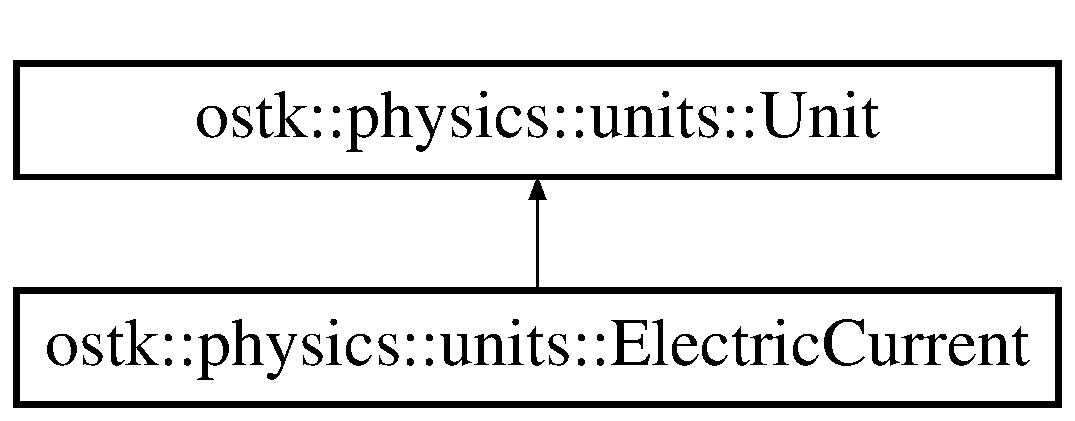
\includegraphics[height=2.000000cm]{classostk_1_1physics_1_1units_1_1_electric_current}
\end{center}
\end{figure}
\subsection*{Public Types}
\begin{DoxyCompactItemize}
\item 
enum \hyperlink{classostk_1_1physics_1_1units_1_1_electric_current_ac57c87a7533dc73b87185b0d9ae6985b}{Unit} \{ \hyperlink{classostk_1_1physics_1_1units_1_1_electric_current_ac57c87a7533dc73b87185b0d9ae6985baec0fc0100c4fc1ce4eea230c3dc10360}{Unit\+::\+Undefined}, 
\hyperlink{classostk_1_1physics_1_1units_1_1_electric_current_ac57c87a7533dc73b87185b0d9ae6985ba2ee3b9f6a94ce5398d1386f42f9c87ac}{Unit\+::\+Ampere}
 \}
\end{DoxyCompactItemize}
\subsection*{Public Member Functions}
\begin{DoxyCompactItemize}
\item 
\hyperlink{classostk_1_1physics_1_1units_1_1_electric_current_af247c4dcd830d2c20f4ba20fdca555a7}{Electric\+Current} (const Real \&a\+Value, const \hyperlink{classostk_1_1physics_1_1units_1_1_electric_current_ac57c87a7533dc73b87185b0d9ae6985b}{Electric\+Current\+::\+Unit} \&a\+Unit)
\begin{DoxyCompactList}\small\item\em Constructor. \end{DoxyCompactList}\item 
virtual \hyperlink{classostk_1_1physics_1_1units_1_1_electric_current}{Electric\+Current} $\ast$ \hyperlink{classostk_1_1physics_1_1units_1_1_electric_current_ac8a261411dee39c74bc43201e8e9c9dd}{clone} () const override
\item 
virtual bool \hyperlink{classostk_1_1physics_1_1units_1_1_electric_current_a81ae490a737a49553a7c390b865486a7}{is\+Defined} () const override
\item 
\hyperlink{classostk_1_1physics_1_1units_1_1_electric_current_ac57c87a7533dc73b87185b0d9ae6985b}{Electric\+Current\+::\+Unit} \hyperlink{classostk_1_1physics_1_1units_1_1_electric_current_a3710fc8f80441eee27bc952ff35a84cd}{get\+Unit} () const
\item 
Real \hyperlink{classostk_1_1physics_1_1units_1_1_electric_current_a8ad14eb9b06b85b372307da5de177899}{in} (const \hyperlink{classostk_1_1physics_1_1units_1_1_electric_current_ac57c87a7533dc73b87185b0d9ae6985b}{Electric\+Current\+::\+Unit} \&a\+Unit) const
\item 
Real \hyperlink{classostk_1_1physics_1_1units_1_1_electric_current_a8f85bb1ad0cac0edaeef92988e66d08b}{in\+Amperes} () const
\item 
virtual String \hyperlink{classostk_1_1physics_1_1units_1_1_electric_current_aa720f442c93f18f81ad769edbd570bd5}{to\+String} (const Integer \&a\+Precision=Integer\+::\+Undefined()) const override
\end{DoxyCompactItemize}
\subsection*{Static Public Member Functions}
\begin{DoxyCompactItemize}
\item 
static \hyperlink{classostk_1_1physics_1_1units_1_1_electric_current}{Electric\+Current} \hyperlink{classostk_1_1physics_1_1units_1_1_electric_current_a1677d42ac10b4fa38624b865f8e097ff}{Undefined} ()
\item 
static \hyperlink{classostk_1_1physics_1_1units_1_1_electric_current}{Electric\+Current} \hyperlink{classostk_1_1physics_1_1units_1_1_electric_current_aea20319b4f2f5e3a312af69baa3bd657}{Amperes} (const Real \&a\+Value)
\item 
static \hyperlink{classostk_1_1physics_1_1units_1_1_electric_current}{Electric\+Current} \hyperlink{classostk_1_1physics_1_1units_1_1_electric_current_ae7e0f9395409e3591e31acb853e846db}{Parse} (const String \&a\+String)
\item 
static String \hyperlink{classostk_1_1physics_1_1units_1_1_electric_current_a89a2bfd34bd35db99c381a27fe969e5c}{String\+From\+Unit} (const \hyperlink{classostk_1_1physics_1_1units_1_1_electric_current_ac57c87a7533dc73b87185b0d9ae6985b}{Electric\+Current\+::\+Unit} \&a\+Unit)
\item 
static String \hyperlink{classostk_1_1physics_1_1units_1_1_electric_current_a3e1d115ee8e8eb80ec72dab5dea37ad1}{Symbol\+From\+Unit} (const \hyperlink{classostk_1_1physics_1_1units_1_1_electric_current_ac57c87a7533dc73b87185b0d9ae6985b}{Electric\+Current\+::\+Unit} \&a\+Unit)
\end{DoxyCompactItemize}
\subsection*{Additional Inherited Members}


\subsection{Detailed Description}
Electric current. 

https\+://en.wikipedia.\+org/wiki/\+Electric\+\_\+current 

\subsection{Member Enumeration Documentation}
\mbox{\Hypertarget{classostk_1_1physics_1_1units_1_1_electric_current_ac57c87a7533dc73b87185b0d9ae6985b}\label{classostk_1_1physics_1_1units_1_1_electric_current_ac57c87a7533dc73b87185b0d9ae6985b}} 
\index{ostk\+::physics\+::units\+::\+Electric\+Current@{ostk\+::physics\+::units\+::\+Electric\+Current}!Unit@{Unit}}
\index{Unit@{Unit}!ostk\+::physics\+::units\+::\+Electric\+Current@{ostk\+::physics\+::units\+::\+Electric\+Current}}
\subsubsection{\texorpdfstring{Unit}{Unit}}
{\footnotesize\ttfamily enum \hyperlink{classostk_1_1physics_1_1units_1_1_electric_current_ac57c87a7533dc73b87185b0d9ae6985b}{ostk\+::physics\+::units\+::\+Electric\+Current\+::\+Unit}\hspace{0.3cm}{\ttfamily [strong]}}

\begin{DoxyEnumFields}{Enumerator}
\raisebox{\heightof{T}}[0pt][0pt]{\index{Undefined@{Undefined}!ostk\+::physics\+::units\+::\+Electric\+Current@{ostk\+::physics\+::units\+::\+Electric\+Current}}\index{ostk\+::physics\+::units\+::\+Electric\+Current@{ostk\+::physics\+::units\+::\+Electric\+Current}!Undefined@{Undefined}}}\mbox{\Hypertarget{classostk_1_1physics_1_1units_1_1_electric_current_ac57c87a7533dc73b87185b0d9ae6985baec0fc0100c4fc1ce4eea230c3dc10360}\label{classostk_1_1physics_1_1units_1_1_electric_current_ac57c87a7533dc73b87185b0d9ae6985baec0fc0100c4fc1ce4eea230c3dc10360}} 
Undefined&Undefined. \\
\hline

\raisebox{\heightof{T}}[0pt][0pt]{\index{Ampere@{Ampere}!ostk\+::physics\+::units\+::\+Electric\+Current@{ostk\+::physics\+::units\+::\+Electric\+Current}}\index{ostk\+::physics\+::units\+::\+Electric\+Current@{ostk\+::physics\+::units\+::\+Electric\+Current}!Ampere@{Ampere}}}\mbox{\Hypertarget{classostk_1_1physics_1_1units_1_1_electric_current_ac57c87a7533dc73b87185b0d9ae6985ba2ee3b9f6a94ce5398d1386f42f9c87ac}\label{classostk_1_1physics_1_1units_1_1_electric_current_ac57c87a7533dc73b87185b0d9ae6985ba2ee3b9f6a94ce5398d1386f42f9c87ac}} 
Ampere&Ampere (SI) \\
\hline

\end{DoxyEnumFields}


\subsection{Constructor \& Destructor Documentation}
\mbox{\Hypertarget{classostk_1_1physics_1_1units_1_1_electric_current_af247c4dcd830d2c20f4ba20fdca555a7}\label{classostk_1_1physics_1_1units_1_1_electric_current_af247c4dcd830d2c20f4ba20fdca555a7}} 
\index{ostk\+::physics\+::units\+::\+Electric\+Current@{ostk\+::physics\+::units\+::\+Electric\+Current}!Electric\+Current@{Electric\+Current}}
\index{Electric\+Current@{Electric\+Current}!ostk\+::physics\+::units\+::\+Electric\+Current@{ostk\+::physics\+::units\+::\+Electric\+Current}}
\subsubsection{\texorpdfstring{Electric\+Current()}{ElectricCurrent()}}
{\footnotesize\ttfamily ostk\+::physics\+::units\+::\+Electric\+Current\+::\+Electric\+Current (\begin{DoxyParamCaption}\item[{const Real \&}]{a\+Value,  }\item[{const \hyperlink{classostk_1_1physics_1_1units_1_1_electric_current_ac57c87a7533dc73b87185b0d9ae6985b}{Electric\+Current\+::\+Unit} \&}]{a\+Unit }\end{DoxyParamCaption})}



Constructor. 


\begin{DoxyCode}
\hyperlink{classostk_1_1physics_1_1units_1_1_electric_current_af247c4dcd830d2c20f4ba20fdca555a7}{ElectricCurrent} electricCurrent \{ 1.0, 
      \hyperlink{classostk_1_1physics_1_1units_1_1_electric_current_ac57c87a7533dc73b87185b0d9ae6985ba2ee3b9f6a94ce5398d1386f42f9c87ac}{ElectricCurrent::Unit::Ampere} \} ;
\end{DoxyCode}



\begin{DoxyParams}[1]{Parameters}
\mbox{\tt in}  & {\em a\+Value} & A value \\
\hline
\mbox{\tt in}  & {\em a\+Unit} & An electric current unit \\
\hline
\end{DoxyParams}


\subsection{Member Function Documentation}
\mbox{\Hypertarget{classostk_1_1physics_1_1units_1_1_electric_current_aea20319b4f2f5e3a312af69baa3bd657}\label{classostk_1_1physics_1_1units_1_1_electric_current_aea20319b4f2f5e3a312af69baa3bd657}} 
\index{ostk\+::physics\+::units\+::\+Electric\+Current@{ostk\+::physics\+::units\+::\+Electric\+Current}!Amperes@{Amperes}}
\index{Amperes@{Amperes}!ostk\+::physics\+::units\+::\+Electric\+Current@{ostk\+::physics\+::units\+::\+Electric\+Current}}
\subsubsection{\texorpdfstring{Amperes()}{Amperes()}}
{\footnotesize\ttfamily \hyperlink{classostk_1_1physics_1_1units_1_1_electric_current}{Electric\+Current} ostk\+::physics\+::units\+::\+Electric\+Current\+::\+Amperes (\begin{DoxyParamCaption}\item[{const Real \&}]{a\+Value }\end{DoxyParamCaption})\hspace{0.3cm}{\ttfamily [static]}}

\mbox{\Hypertarget{classostk_1_1physics_1_1units_1_1_electric_current_ac8a261411dee39c74bc43201e8e9c9dd}\label{classostk_1_1physics_1_1units_1_1_electric_current_ac8a261411dee39c74bc43201e8e9c9dd}} 
\index{ostk\+::physics\+::units\+::\+Electric\+Current@{ostk\+::physics\+::units\+::\+Electric\+Current}!clone@{clone}}
\index{clone@{clone}!ostk\+::physics\+::units\+::\+Electric\+Current@{ostk\+::physics\+::units\+::\+Electric\+Current}}
\subsubsection{\texorpdfstring{clone()}{clone()}}
{\footnotesize\ttfamily \hyperlink{classostk_1_1physics_1_1units_1_1_electric_current}{Electric\+Current} $\ast$ ostk\+::physics\+::units\+::\+Electric\+Current\+::clone (\begin{DoxyParamCaption}{ }\end{DoxyParamCaption}) const\hspace{0.3cm}{\ttfamily [override]}, {\ttfamily [virtual]}}



Implements \hyperlink{classostk_1_1physics_1_1units_1_1_unit_ab203628f8a16b16c28d89eaa4c3aff67}{ostk\+::physics\+::units\+::\+Unit}.

\mbox{\Hypertarget{classostk_1_1physics_1_1units_1_1_electric_current_a3710fc8f80441eee27bc952ff35a84cd}\label{classostk_1_1physics_1_1units_1_1_electric_current_a3710fc8f80441eee27bc952ff35a84cd}} 
\index{ostk\+::physics\+::units\+::\+Electric\+Current@{ostk\+::physics\+::units\+::\+Electric\+Current}!get\+Unit@{get\+Unit}}
\index{get\+Unit@{get\+Unit}!ostk\+::physics\+::units\+::\+Electric\+Current@{ostk\+::physics\+::units\+::\+Electric\+Current}}
\subsubsection{\texorpdfstring{get\+Unit()}{getUnit()}}
{\footnotesize\ttfamily \hyperlink{classostk_1_1physics_1_1units_1_1_electric_current_ac57c87a7533dc73b87185b0d9ae6985b}{Electric\+Current\+::\+Unit} ostk\+::physics\+::units\+::\+Electric\+Current\+::get\+Unit (\begin{DoxyParamCaption}{ }\end{DoxyParamCaption}) const}

\mbox{\Hypertarget{classostk_1_1physics_1_1units_1_1_electric_current_a8ad14eb9b06b85b372307da5de177899}\label{classostk_1_1physics_1_1units_1_1_electric_current_a8ad14eb9b06b85b372307da5de177899}} 
\index{ostk\+::physics\+::units\+::\+Electric\+Current@{ostk\+::physics\+::units\+::\+Electric\+Current}!in@{in}}
\index{in@{in}!ostk\+::physics\+::units\+::\+Electric\+Current@{ostk\+::physics\+::units\+::\+Electric\+Current}}
\subsubsection{\texorpdfstring{in()}{in()}}
{\footnotesize\ttfamily Real ostk\+::physics\+::units\+::\+Electric\+Current\+::in (\begin{DoxyParamCaption}\item[{const \hyperlink{classostk_1_1physics_1_1units_1_1_electric_current_ac57c87a7533dc73b87185b0d9ae6985b}{Electric\+Current\+::\+Unit} \&}]{a\+Unit }\end{DoxyParamCaption}) const}

\mbox{\Hypertarget{classostk_1_1physics_1_1units_1_1_electric_current_a8f85bb1ad0cac0edaeef92988e66d08b}\label{classostk_1_1physics_1_1units_1_1_electric_current_a8f85bb1ad0cac0edaeef92988e66d08b}} 
\index{ostk\+::physics\+::units\+::\+Electric\+Current@{ostk\+::physics\+::units\+::\+Electric\+Current}!in\+Amperes@{in\+Amperes}}
\index{in\+Amperes@{in\+Amperes}!ostk\+::physics\+::units\+::\+Electric\+Current@{ostk\+::physics\+::units\+::\+Electric\+Current}}
\subsubsection{\texorpdfstring{in\+Amperes()}{inAmperes()}}
{\footnotesize\ttfamily Real ostk\+::physics\+::units\+::\+Electric\+Current\+::in\+Amperes (\begin{DoxyParamCaption}{ }\end{DoxyParamCaption}) const}

\mbox{\Hypertarget{classostk_1_1physics_1_1units_1_1_electric_current_a81ae490a737a49553a7c390b865486a7}\label{classostk_1_1physics_1_1units_1_1_electric_current_a81ae490a737a49553a7c390b865486a7}} 
\index{ostk\+::physics\+::units\+::\+Electric\+Current@{ostk\+::physics\+::units\+::\+Electric\+Current}!is\+Defined@{is\+Defined}}
\index{is\+Defined@{is\+Defined}!ostk\+::physics\+::units\+::\+Electric\+Current@{ostk\+::physics\+::units\+::\+Electric\+Current}}
\subsubsection{\texorpdfstring{is\+Defined()}{isDefined()}}
{\footnotesize\ttfamily bool ostk\+::physics\+::units\+::\+Electric\+Current\+::is\+Defined (\begin{DoxyParamCaption}{ }\end{DoxyParamCaption}) const\hspace{0.3cm}{\ttfamily [override]}, {\ttfamily [virtual]}}



Reimplemented from \hyperlink{classostk_1_1physics_1_1units_1_1_unit_a423ce1df3478f0892b10824b591ae1cc}{ostk\+::physics\+::units\+::\+Unit}.

\mbox{\Hypertarget{classostk_1_1physics_1_1units_1_1_electric_current_ae7e0f9395409e3591e31acb853e846db}\label{classostk_1_1physics_1_1units_1_1_electric_current_ae7e0f9395409e3591e31acb853e846db}} 
\index{ostk\+::physics\+::units\+::\+Electric\+Current@{ostk\+::physics\+::units\+::\+Electric\+Current}!Parse@{Parse}}
\index{Parse@{Parse}!ostk\+::physics\+::units\+::\+Electric\+Current@{ostk\+::physics\+::units\+::\+Electric\+Current}}
\subsubsection{\texorpdfstring{Parse()}{Parse()}}
{\footnotesize\ttfamily static \hyperlink{classostk_1_1physics_1_1units_1_1_electric_current}{Electric\+Current} ostk\+::physics\+::units\+::\+Electric\+Current\+::\+Parse (\begin{DoxyParamCaption}\item[{const String \&}]{a\+String }\end{DoxyParamCaption})\hspace{0.3cm}{\ttfamily [static]}}

\mbox{\Hypertarget{classostk_1_1physics_1_1units_1_1_electric_current_a89a2bfd34bd35db99c381a27fe969e5c}\label{classostk_1_1physics_1_1units_1_1_electric_current_a89a2bfd34bd35db99c381a27fe969e5c}} 
\index{ostk\+::physics\+::units\+::\+Electric\+Current@{ostk\+::physics\+::units\+::\+Electric\+Current}!String\+From\+Unit@{String\+From\+Unit}}
\index{String\+From\+Unit@{String\+From\+Unit}!ostk\+::physics\+::units\+::\+Electric\+Current@{ostk\+::physics\+::units\+::\+Electric\+Current}}
\subsubsection{\texorpdfstring{String\+From\+Unit()}{StringFromUnit()}}
{\footnotesize\ttfamily String ostk\+::physics\+::units\+::\+Electric\+Current\+::\+String\+From\+Unit (\begin{DoxyParamCaption}\item[{const \hyperlink{classostk_1_1physics_1_1units_1_1_electric_current_ac57c87a7533dc73b87185b0d9ae6985b}{Electric\+Current\+::\+Unit} \&}]{a\+Unit }\end{DoxyParamCaption})\hspace{0.3cm}{\ttfamily [static]}}

\mbox{\Hypertarget{classostk_1_1physics_1_1units_1_1_electric_current_a3e1d115ee8e8eb80ec72dab5dea37ad1}\label{classostk_1_1physics_1_1units_1_1_electric_current_a3e1d115ee8e8eb80ec72dab5dea37ad1}} 
\index{ostk\+::physics\+::units\+::\+Electric\+Current@{ostk\+::physics\+::units\+::\+Electric\+Current}!Symbol\+From\+Unit@{Symbol\+From\+Unit}}
\index{Symbol\+From\+Unit@{Symbol\+From\+Unit}!ostk\+::physics\+::units\+::\+Electric\+Current@{ostk\+::physics\+::units\+::\+Electric\+Current}}
\subsubsection{\texorpdfstring{Symbol\+From\+Unit()}{SymbolFromUnit()}}
{\footnotesize\ttfamily String ostk\+::physics\+::units\+::\+Electric\+Current\+::\+Symbol\+From\+Unit (\begin{DoxyParamCaption}\item[{const \hyperlink{classostk_1_1physics_1_1units_1_1_electric_current_ac57c87a7533dc73b87185b0d9ae6985b}{Electric\+Current\+::\+Unit} \&}]{a\+Unit }\end{DoxyParamCaption})\hspace{0.3cm}{\ttfamily [static]}}

\mbox{\Hypertarget{classostk_1_1physics_1_1units_1_1_electric_current_aa720f442c93f18f81ad769edbd570bd5}\label{classostk_1_1physics_1_1units_1_1_electric_current_aa720f442c93f18f81ad769edbd570bd5}} 
\index{ostk\+::physics\+::units\+::\+Electric\+Current@{ostk\+::physics\+::units\+::\+Electric\+Current}!to\+String@{to\+String}}
\index{to\+String@{to\+String}!ostk\+::physics\+::units\+::\+Electric\+Current@{ostk\+::physics\+::units\+::\+Electric\+Current}}
\subsubsection{\texorpdfstring{to\+String()}{toString()}}
{\footnotesize\ttfamily String ostk\+::physics\+::units\+::\+Electric\+Current\+::to\+String (\begin{DoxyParamCaption}\item[{const Integer \&}]{a\+Precision = {\ttfamily Integer\+:\+:Undefined()} }\end{DoxyParamCaption}) const\hspace{0.3cm}{\ttfamily [override]}, {\ttfamily [virtual]}}



Implements \hyperlink{classostk_1_1physics_1_1units_1_1_unit_a8162b4eb8221c7577af16ab8b399d07e}{ostk\+::physics\+::units\+::\+Unit}.

\mbox{\Hypertarget{classostk_1_1physics_1_1units_1_1_electric_current_a1677d42ac10b4fa38624b865f8e097ff}\label{classostk_1_1physics_1_1units_1_1_electric_current_a1677d42ac10b4fa38624b865f8e097ff}} 
\index{ostk\+::physics\+::units\+::\+Electric\+Current@{ostk\+::physics\+::units\+::\+Electric\+Current}!Undefined@{Undefined}}
\index{Undefined@{Undefined}!ostk\+::physics\+::units\+::\+Electric\+Current@{ostk\+::physics\+::units\+::\+Electric\+Current}}
\subsubsection{\texorpdfstring{Undefined()}{Undefined()}}
{\footnotesize\ttfamily \hyperlink{classostk_1_1physics_1_1units_1_1_electric_current}{Electric\+Current} ostk\+::physics\+::units\+::\+Electric\+Current\+::\+Undefined (\begin{DoxyParamCaption}{ }\end{DoxyParamCaption})\hspace{0.3cm}{\ttfamily [static]}}



The documentation for this class was generated from the following files\+:\begin{DoxyCompactItemize}
\item 
include/\+Open\+Space\+Toolkit/\+Physics/\+Units/\hyperlink{_electric_current_8hpp}{Electric\+Current.\+hpp}\item 
src/\+Open\+Space\+Toolkit/\+Physics/\+Units/\hyperlink{_electric_current_8cpp}{Electric\+Current.\+cpp}\end{DoxyCompactItemize}

\hypertarget{classostk_1_1physics_1_1env_1_1ephem_1_1spice_1_1_engine}{}\section{ostk\+:\+:physics\+:\+:env\+:\+:ephem\+:\+:spice\+:\+:Engine Class Reference}
\label{classostk_1_1physics_1_1env_1_1ephem_1_1spice_1_1_engine}\index{ostk\+::physics\+::env\+::ephem\+::spice\+::\+Engine@{ostk\+::physics\+::env\+::ephem\+::spice\+::\+Engine}}


\hyperlink{classostk_1_1physics_1_1env_1_1ephem_1_1_s_p_i_c_e}{S\+P\+I\+CE} Toolkit engine.  




{\ttfamily \#include $<$Engine.\+hpp$>$}

\subsection*{Public Types}
\begin{DoxyCompactItemize}
\item 
enum \hyperlink{classostk_1_1physics_1_1env_1_1ephem_1_1spice_1_1_engine_a803b82d8f41c81e861852098b6b75ae2}{Mode} \{ \hyperlink{classostk_1_1physics_1_1env_1_1ephem_1_1spice_1_1_engine_a803b82d8f41c81e861852098b6b75ae2ae1ba155a9f2e8c3be94020eef32a0301}{Mode\+::\+Manual}, 
\hyperlink{classostk_1_1physics_1_1env_1_1ephem_1_1spice_1_1_engine_a803b82d8f41c81e861852098b6b75ae2a086247a9b57fde6eefee2a0c4752242d}{Mode\+::\+Automatic}
 \}\begin{DoxyCompactList}\small\item\em \hyperlink{classostk_1_1physics_1_1env_1_1ephem_1_1spice_1_1_engine}{Engine} mode. \end{DoxyCompactList}
\end{DoxyCompactItemize}
\subsection*{Public Member Functions}
\begin{DoxyCompactItemize}
\item 
\hyperlink{classostk_1_1physics_1_1env_1_1ephem_1_1spice_1_1_engine_a60734f4383f29cfaaaa50126fef0ceb5}{Engine} (const \hyperlink{classostk_1_1physics_1_1env_1_1ephem_1_1spice_1_1_engine}{Engine} \&a\+Spice\+Engine)=delete
\begin{DoxyCompactList}\small\item\em Copy constructor (deleted) \end{DoxyCompactList}\item 
\hyperlink{classostk_1_1physics_1_1env_1_1ephem_1_1spice_1_1_engine}{Engine} \& \hyperlink{classostk_1_1physics_1_1env_1_1ephem_1_1spice_1_1_engine_a807af40bbe562341a66abb875fa3ab9f}{operator=} (const \hyperlink{classostk_1_1physics_1_1env_1_1ephem_1_1spice_1_1_engine}{Engine} \&a\+Spice\+Engine)=delete
\begin{DoxyCompactList}\small\item\em Copy assignment operator (deleted) \end{DoxyCompactList}\item 
bool \hyperlink{classostk_1_1physics_1_1env_1_1ephem_1_1spice_1_1_engine_aeb4efb8c50f73b90083ebd7d8a5e317f}{is\+Kernel\+Loaded} (const \hyperlink{classostk_1_1physics_1_1env_1_1ephem_1_1spice_1_1_kernel}{Kernel} \&a\+Kernel) const
\begin{DoxyCompactList}\small\item\em Returns true if kernel is loaded. \end{DoxyCompactList}\item 
\hyperlink{classostk_1_1physics_1_1env_1_1ephem_1_1spice_1_1_engine_a803b82d8f41c81e861852098b6b75ae2}{Engine\+::\+Mode} \hyperlink{classostk_1_1physics_1_1env_1_1ephem_1_1spice_1_1_engine_af7d9d424721bc7bc9d634c00699c897c}{get\+Mode} () const
\begin{DoxyCompactList}\small\item\em Get engine mode. \end{DoxyCompactList}\item 
Shared$<$ const \hyperlink{classostk_1_1physics_1_1coord_1_1_frame}{Frame} $>$ \hyperlink{classostk_1_1physics_1_1env_1_1ephem_1_1spice_1_1_engine_aeffd094033f2bd2c276b9d9a9840d7ea}{get\+Frame\+Of} (const \hyperlink{classostk_1_1physics_1_1env_1_1ephem_1_1_s_p_i_c_e_ae84db78d858cdd0a1dc3ff53090f4a1f}{S\+P\+I\+C\+E\+::\+Object} \&a\+Spice\+Object) const
\begin{DoxyCompactList}\small\item\em Get frame of \hyperlink{classostk_1_1physics_1_1env_1_1ephem_1_1_s_p_i_c_e}{S\+P\+I\+CE} object. \end{DoxyCompactList}\item 
void \hyperlink{classostk_1_1physics_1_1env_1_1ephem_1_1spice_1_1_engine_a5927d9c72c81334dcb0d8fa9ba20158e}{set\+Mode} (const \hyperlink{classostk_1_1physics_1_1env_1_1ephem_1_1spice_1_1_engine_a803b82d8f41c81e861852098b6b75ae2}{Engine\+::\+Mode} \&a\+Mode)
\begin{DoxyCompactList}\small\item\em Set engine mode. \end{DoxyCompactList}\item 
void \hyperlink{classostk_1_1physics_1_1env_1_1ephem_1_1spice_1_1_engine_aa1aa0d1e376b18899c603950a2d43589}{load\+Kernel} (const \hyperlink{classostk_1_1physics_1_1env_1_1ephem_1_1spice_1_1_kernel}{Kernel} \&a\+Kernel)
\begin{DoxyCompactList}\small\item\em Load kernel. \end{DoxyCompactList}\item 
void \hyperlink{classostk_1_1physics_1_1env_1_1ephem_1_1spice_1_1_engine_a6aa17a14f23f01dddba741a55307b8f9}{unload\+Kernel} (const \hyperlink{classostk_1_1physics_1_1env_1_1ephem_1_1spice_1_1_kernel}{Kernel} \&a\+Kernel)
\begin{DoxyCompactList}\small\item\em Unload kernel. \end{DoxyCompactList}\item 
void \hyperlink{classostk_1_1physics_1_1env_1_1ephem_1_1spice_1_1_engine_ad459dacf25f4ba08089b5d1111ca7814}{reset} ()
\begin{DoxyCompactList}\small\item\em Reset engine. \end{DoxyCompactList}\end{DoxyCompactItemize}
\subsection*{Static Public Member Functions}
\begin{DoxyCompactItemize}
\item 
static \hyperlink{classostk_1_1physics_1_1env_1_1ephem_1_1spice_1_1_engine}{Engine} \& \hyperlink{classostk_1_1physics_1_1env_1_1ephem_1_1spice_1_1_engine_a98ce9249db18853920308c699fbca541}{Get} ()
\begin{DoxyCompactList}\small\item\em Get engine singleton. \end{DoxyCompactList}\item 
static \hyperlink{classostk_1_1physics_1_1env_1_1ephem_1_1spice_1_1_engine_a803b82d8f41c81e861852098b6b75ae2}{Engine\+::\+Mode} \hyperlink{classostk_1_1physics_1_1env_1_1ephem_1_1spice_1_1_engine_a6b8bdf7ead864216cd07fc9d81fab39b}{Default\+Mode} ()
\begin{DoxyCompactList}\small\item\em Get default engine mode. \end{DoxyCompactList}\item 
static Array$<$ \hyperlink{classostk_1_1physics_1_1env_1_1ephem_1_1spice_1_1_kernel}{Kernel} $>$ \hyperlink{classostk_1_1physics_1_1env_1_1ephem_1_1spice_1_1_engine_a719948b0aaa86f50f832db8488c5b1f2}{Default\+Kernels} (const Directory \&a\+Local\+Repository)
\begin{DoxyCompactList}\small\item\em Get default kernels. \end{DoxyCompactList}\end{DoxyCompactItemize}
\subsection*{Friends}
\begin{DoxyCompactItemize}
\item 
std\+::ostream \& \hyperlink{classostk_1_1physics_1_1env_1_1ephem_1_1spice_1_1_engine_a880dd680a3b5444757480fafd1a52679}{operator$<$$<$} (std\+::ostream \&an\+Output\+Stream, const \hyperlink{classostk_1_1physics_1_1env_1_1ephem_1_1spice_1_1_engine}{Engine} \&an\+Engine)
\begin{DoxyCompactList}\small\item\em Output stream operator. \end{DoxyCompactList}\end{DoxyCompactItemize}


\subsection{Detailed Description}
\hyperlink{classostk_1_1physics_1_1env_1_1ephem_1_1_s_p_i_c_e}{S\+P\+I\+CE} Toolkit engine. 

The following environment variables can be defined\+:


\begin{DoxyItemize}
\item \char`\"{}\+L\+I\+B\+R\+A\+R\+Y\+\_\+\+P\+H\+Y\+S\+I\+C\+S\+\_\+\+E\+N\+V\+I\+R\+O\+N\+M\+E\+N\+T\+\_\+\+E\+P\+H\+E\+M\+E\+R\+I\+D\+E\+S\+\_\+\+S\+P\+I\+C\+E\+\_\+\+E\+N\+G\+I\+N\+E\+\_\+\+M\+O\+D\+E\char`\"{} will override \char`\"{}\+Default\+Mode\char`\"{} 
\end{DoxyItemize}

\subsection{Member Enumeration Documentation}
\mbox{\Hypertarget{classostk_1_1physics_1_1env_1_1ephem_1_1spice_1_1_engine_a803b82d8f41c81e861852098b6b75ae2}\label{classostk_1_1physics_1_1env_1_1ephem_1_1spice_1_1_engine_a803b82d8f41c81e861852098b6b75ae2}} 
\index{ostk\+::physics\+::env\+::ephem\+::spice\+::\+Engine@{ostk\+::physics\+::env\+::ephem\+::spice\+::\+Engine}!Mode@{Mode}}
\index{Mode@{Mode}!ostk\+::physics\+::env\+::ephem\+::spice\+::\+Engine@{ostk\+::physics\+::env\+::ephem\+::spice\+::\+Engine}}
\subsubsection{\texorpdfstring{Mode}{Mode}}
{\footnotesize\ttfamily enum \hyperlink{classostk_1_1physics_1_1env_1_1ephem_1_1spice_1_1_engine_a803b82d8f41c81e861852098b6b75ae2}{ostk\+::physics\+::env\+::ephem\+::spice\+::\+Engine\+::\+Mode}\hspace{0.3cm}{\ttfamily [strong]}}



\hyperlink{classostk_1_1physics_1_1env_1_1ephem_1_1spice_1_1_engine}{Engine} mode. 

\begin{DoxyEnumFields}{Enumerator}
\raisebox{\heightof{T}}[0pt][0pt]{\index{Manual@{Manual}!ostk\+::physics\+::env\+::ephem\+::spice\+::\+Engine@{ostk\+::physics\+::env\+::ephem\+::spice\+::\+Engine}}\index{ostk\+::physics\+::env\+::ephem\+::spice\+::\+Engine@{ostk\+::physics\+::env\+::ephem\+::spice\+::\+Engine}!Manual@{Manual}}}\mbox{\Hypertarget{classostk_1_1physics_1_1env_1_1ephem_1_1spice_1_1_engine_a803b82d8f41c81e861852098b6b75ae2ae1ba155a9f2e8c3be94020eef32a0301}\label{classostk_1_1physics_1_1env_1_1ephem_1_1spice_1_1_engine_a803b82d8f41c81e861852098b6b75ae2ae1ba155a9f2e8c3be94020eef32a0301}} 
Manual&Manually load and unload kernels. \\
\hline

\raisebox{\heightof{T}}[0pt][0pt]{\index{Automatic@{Automatic}!ostk\+::physics\+::env\+::ephem\+::spice\+::\+Engine@{ostk\+::physics\+::env\+::ephem\+::spice\+::\+Engine}}\index{ostk\+::physics\+::env\+::ephem\+::spice\+::\+Engine@{ostk\+::physics\+::env\+::ephem\+::spice\+::\+Engine}!Automatic@{Automatic}}}\mbox{\Hypertarget{classostk_1_1physics_1_1env_1_1ephem_1_1spice_1_1_engine_a803b82d8f41c81e861852098b6b75ae2a086247a9b57fde6eefee2a0c4752242d}\label{classostk_1_1physics_1_1env_1_1ephem_1_1spice_1_1_engine_a803b82d8f41c81e861852098b6b75ae2a086247a9b57fde6eefee2a0c4752242d}} 
Automatic&Automatically fetch, load and unload kernels (from remote repositories) \\
\hline

\end{DoxyEnumFields}


\subsection{Constructor \& Destructor Documentation}
\mbox{\Hypertarget{classostk_1_1physics_1_1env_1_1ephem_1_1spice_1_1_engine_a60734f4383f29cfaaaa50126fef0ceb5}\label{classostk_1_1physics_1_1env_1_1ephem_1_1spice_1_1_engine_a60734f4383f29cfaaaa50126fef0ceb5}} 
\index{ostk\+::physics\+::env\+::ephem\+::spice\+::\+Engine@{ostk\+::physics\+::env\+::ephem\+::spice\+::\+Engine}!Engine@{Engine}}
\index{Engine@{Engine}!ostk\+::physics\+::env\+::ephem\+::spice\+::\+Engine@{ostk\+::physics\+::env\+::ephem\+::spice\+::\+Engine}}
\subsubsection{\texorpdfstring{Engine()}{Engine()}}
{\footnotesize\ttfamily ostk\+::physics\+::env\+::ephem\+::spice\+::\+Engine\+::\+Engine (\begin{DoxyParamCaption}\item[{const \hyperlink{classostk_1_1physics_1_1env_1_1ephem_1_1spice_1_1_engine}{Engine} \&}]{a\+Spice\+Engine }\end{DoxyParamCaption})\hspace{0.3cm}{\ttfamily [delete]}}



Copy constructor (deleted) 



\subsection{Member Function Documentation}
\mbox{\Hypertarget{classostk_1_1physics_1_1env_1_1ephem_1_1spice_1_1_engine_a719948b0aaa86f50f832db8488c5b1f2}\label{classostk_1_1physics_1_1env_1_1ephem_1_1spice_1_1_engine_a719948b0aaa86f50f832db8488c5b1f2}} 
\index{ostk\+::physics\+::env\+::ephem\+::spice\+::\+Engine@{ostk\+::physics\+::env\+::ephem\+::spice\+::\+Engine}!Default\+Kernels@{Default\+Kernels}}
\index{Default\+Kernels@{Default\+Kernels}!ostk\+::physics\+::env\+::ephem\+::spice\+::\+Engine@{ostk\+::physics\+::env\+::ephem\+::spice\+::\+Engine}}
\subsubsection{\texorpdfstring{Default\+Kernels()}{DefaultKernels()}}
{\footnotesize\ttfamily Array$<$ \hyperlink{classostk_1_1physics_1_1env_1_1ephem_1_1spice_1_1_kernel}{Kernel} $>$ ostk\+::physics\+::env\+::ephem\+::spice\+::\+Engine\+::\+Default\+Kernels (\begin{DoxyParamCaption}\item[{const Directory \&}]{a\+Local\+Repository }\end{DoxyParamCaption})\hspace{0.3cm}{\ttfamily [static]}}



Get default kernels. 


\begin{DoxyParams}[1]{Parameters}
\mbox{\tt in}  & {\em a\+Local\+Repository} & A local repository \\
\hline
\end{DoxyParams}
\begin{DoxyReturn}{Returns}
Default kernels 
\end{DoxyReturn}
\mbox{\Hypertarget{classostk_1_1physics_1_1env_1_1ephem_1_1spice_1_1_engine_a6b8bdf7ead864216cd07fc9d81fab39b}\label{classostk_1_1physics_1_1env_1_1ephem_1_1spice_1_1_engine_a6b8bdf7ead864216cd07fc9d81fab39b}} 
\index{ostk\+::physics\+::env\+::ephem\+::spice\+::\+Engine@{ostk\+::physics\+::env\+::ephem\+::spice\+::\+Engine}!Default\+Mode@{Default\+Mode}}
\index{Default\+Mode@{Default\+Mode}!ostk\+::physics\+::env\+::ephem\+::spice\+::\+Engine@{ostk\+::physics\+::env\+::ephem\+::spice\+::\+Engine}}
\subsubsection{\texorpdfstring{Default\+Mode()}{DefaultMode()}}
{\footnotesize\ttfamily \hyperlink{classostk_1_1physics_1_1env_1_1ephem_1_1spice_1_1_engine_a803b82d8f41c81e861852098b6b75ae2}{Engine\+::\+Mode} ostk\+::physics\+::env\+::ephem\+::spice\+::\+Engine\+::\+Default\+Mode (\begin{DoxyParamCaption}{ }\end{DoxyParamCaption})\hspace{0.3cm}{\ttfamily [static]}}



Get default engine mode. 

Overriden by\+: L\+I\+B\+R\+A\+R\+Y\+\_\+\+P\+H\+Y\+S\+I\+C\+S\+\_\+\+E\+N\+V\+I\+R\+O\+N\+M\+E\+N\+T\+\_\+\+E\+P\+H\+E\+M\+E\+R\+I\+D\+E\+S\+\_\+\+S\+P\+I\+C\+E\+\_\+\+E\+N\+G\+I\+N\+E\+\_\+\+M\+O\+DE

\begin{DoxyReturn}{Returns}
Default engine mode 
\end{DoxyReturn}
\mbox{\Hypertarget{classostk_1_1physics_1_1env_1_1ephem_1_1spice_1_1_engine_a98ce9249db18853920308c699fbca541}\label{classostk_1_1physics_1_1env_1_1ephem_1_1spice_1_1_engine_a98ce9249db18853920308c699fbca541}} 
\index{ostk\+::physics\+::env\+::ephem\+::spice\+::\+Engine@{ostk\+::physics\+::env\+::ephem\+::spice\+::\+Engine}!Get@{Get}}
\index{Get@{Get}!ostk\+::physics\+::env\+::ephem\+::spice\+::\+Engine@{ostk\+::physics\+::env\+::ephem\+::spice\+::\+Engine}}
\subsubsection{\texorpdfstring{Get()}{Get()}}
{\footnotesize\ttfamily \hyperlink{classostk_1_1physics_1_1env_1_1ephem_1_1spice_1_1_engine}{Engine} \& ostk\+::physics\+::env\+::ephem\+::spice\+::\+Engine\+::\+Get (\begin{DoxyParamCaption}{ }\end{DoxyParamCaption})\hspace{0.3cm}{\ttfamily [static]}}



Get engine singleton. 

\begin{DoxyReturn}{Returns}
Reference to engine 
\end{DoxyReturn}
\mbox{\Hypertarget{classostk_1_1physics_1_1env_1_1ephem_1_1spice_1_1_engine_aeffd094033f2bd2c276b9d9a9840d7ea}\label{classostk_1_1physics_1_1env_1_1ephem_1_1spice_1_1_engine_aeffd094033f2bd2c276b9d9a9840d7ea}} 
\index{ostk\+::physics\+::env\+::ephem\+::spice\+::\+Engine@{ostk\+::physics\+::env\+::ephem\+::spice\+::\+Engine}!get\+Frame\+Of@{get\+Frame\+Of}}
\index{get\+Frame\+Of@{get\+Frame\+Of}!ostk\+::physics\+::env\+::ephem\+::spice\+::\+Engine@{ostk\+::physics\+::env\+::ephem\+::spice\+::\+Engine}}
\subsubsection{\texorpdfstring{get\+Frame\+Of()}{getFrameOf()}}
{\footnotesize\ttfamily Shared$<$ const \hyperlink{classostk_1_1physics_1_1coord_1_1_frame}{Frame} $>$ ostk\+::physics\+::env\+::ephem\+::spice\+::\+Engine\+::get\+Frame\+Of (\begin{DoxyParamCaption}\item[{const \hyperlink{classostk_1_1physics_1_1env_1_1ephem_1_1_s_p_i_c_e_ae84db78d858cdd0a1dc3ff53090f4a1f}{S\+P\+I\+C\+E\+::\+Object} \&}]{a\+Spice\+Object }\end{DoxyParamCaption}) const}



Get frame of \hyperlink{classostk_1_1physics_1_1env_1_1ephem_1_1_s_p_i_c_e}{S\+P\+I\+CE} object. 


\begin{DoxyParams}[1]{Parameters}
\mbox{\tt in}  & {\em A} & \hyperlink{classostk_1_1physics_1_1env_1_1ephem_1_1_s_p_i_c_e}{S\+P\+I\+CE} object \\
\hline
\end{DoxyParams}
\begin{DoxyReturn}{Returns}
Frame of \hyperlink{classostk_1_1physics_1_1env_1_1ephem_1_1_s_p_i_c_e}{S\+P\+I\+CE} object 
\end{DoxyReturn}
\mbox{\Hypertarget{classostk_1_1physics_1_1env_1_1ephem_1_1spice_1_1_engine_af7d9d424721bc7bc9d634c00699c897c}\label{classostk_1_1physics_1_1env_1_1ephem_1_1spice_1_1_engine_af7d9d424721bc7bc9d634c00699c897c}} 
\index{ostk\+::physics\+::env\+::ephem\+::spice\+::\+Engine@{ostk\+::physics\+::env\+::ephem\+::spice\+::\+Engine}!get\+Mode@{get\+Mode}}
\index{get\+Mode@{get\+Mode}!ostk\+::physics\+::env\+::ephem\+::spice\+::\+Engine@{ostk\+::physics\+::env\+::ephem\+::spice\+::\+Engine}}
\subsubsection{\texorpdfstring{get\+Mode()}{getMode()}}
{\footnotesize\ttfamily \hyperlink{classostk_1_1physics_1_1env_1_1ephem_1_1spice_1_1_engine_a803b82d8f41c81e861852098b6b75ae2}{Engine\+::\+Mode} ostk\+::physics\+::env\+::ephem\+::spice\+::\+Engine\+::get\+Mode (\begin{DoxyParamCaption}{ }\end{DoxyParamCaption}) const}



Get engine mode. 

\begin{DoxyReturn}{Returns}
\hyperlink{classostk_1_1physics_1_1env_1_1ephem_1_1spice_1_1_engine}{Engine} mode 
\end{DoxyReturn}
\mbox{\Hypertarget{classostk_1_1physics_1_1env_1_1ephem_1_1spice_1_1_engine_aeb4efb8c50f73b90083ebd7d8a5e317f}\label{classostk_1_1physics_1_1env_1_1ephem_1_1spice_1_1_engine_aeb4efb8c50f73b90083ebd7d8a5e317f}} 
\index{ostk\+::physics\+::env\+::ephem\+::spice\+::\+Engine@{ostk\+::physics\+::env\+::ephem\+::spice\+::\+Engine}!is\+Kernel\+Loaded@{is\+Kernel\+Loaded}}
\index{is\+Kernel\+Loaded@{is\+Kernel\+Loaded}!ostk\+::physics\+::env\+::ephem\+::spice\+::\+Engine@{ostk\+::physics\+::env\+::ephem\+::spice\+::\+Engine}}
\subsubsection{\texorpdfstring{is\+Kernel\+Loaded()}{isKernelLoaded()}}
{\footnotesize\ttfamily bool ostk\+::physics\+::env\+::ephem\+::spice\+::\+Engine\+::is\+Kernel\+Loaded (\begin{DoxyParamCaption}\item[{const \hyperlink{classostk_1_1physics_1_1env_1_1ephem_1_1spice_1_1_kernel}{Kernel} \&}]{a\+Kernel }\end{DoxyParamCaption}) const}



Returns true if kernel is loaded. 


\begin{DoxyParams}[1]{Parameters}
\mbox{\tt in}  & {\em a\+Kernel} & A kernel \\
\hline
\end{DoxyParams}
\begin{DoxyReturn}{Returns}
True if kernel is loaded 
\end{DoxyReturn}
\mbox{\Hypertarget{classostk_1_1physics_1_1env_1_1ephem_1_1spice_1_1_engine_aa1aa0d1e376b18899c603950a2d43589}\label{classostk_1_1physics_1_1env_1_1ephem_1_1spice_1_1_engine_aa1aa0d1e376b18899c603950a2d43589}} 
\index{ostk\+::physics\+::env\+::ephem\+::spice\+::\+Engine@{ostk\+::physics\+::env\+::ephem\+::spice\+::\+Engine}!load\+Kernel@{load\+Kernel}}
\index{load\+Kernel@{load\+Kernel}!ostk\+::physics\+::env\+::ephem\+::spice\+::\+Engine@{ostk\+::physics\+::env\+::ephem\+::spice\+::\+Engine}}
\subsubsection{\texorpdfstring{load\+Kernel()}{loadKernel()}}
{\footnotesize\ttfamily void ostk\+::physics\+::env\+::ephem\+::spice\+::\+Engine\+::load\+Kernel (\begin{DoxyParamCaption}\item[{const \hyperlink{classostk_1_1physics_1_1env_1_1ephem_1_1spice_1_1_kernel}{Kernel} \&}]{a\+Kernel }\end{DoxyParamCaption})}



Load kernel. 


\begin{DoxyParams}[1]{Parameters}
\mbox{\tt in}  & {\em a\+Kernel} & A kernel \\
\hline
\end{DoxyParams}
\mbox{\Hypertarget{classostk_1_1physics_1_1env_1_1ephem_1_1spice_1_1_engine_a807af40bbe562341a66abb875fa3ab9f}\label{classostk_1_1physics_1_1env_1_1ephem_1_1spice_1_1_engine_a807af40bbe562341a66abb875fa3ab9f}} 
\index{ostk\+::physics\+::env\+::ephem\+::spice\+::\+Engine@{ostk\+::physics\+::env\+::ephem\+::spice\+::\+Engine}!operator=@{operator=}}
\index{operator=@{operator=}!ostk\+::physics\+::env\+::ephem\+::spice\+::\+Engine@{ostk\+::physics\+::env\+::ephem\+::spice\+::\+Engine}}
\subsubsection{\texorpdfstring{operator=()}{operator=()}}
{\footnotesize\ttfamily \hyperlink{classostk_1_1physics_1_1env_1_1ephem_1_1spice_1_1_engine}{Engine}\& ostk\+::physics\+::env\+::ephem\+::spice\+::\+Engine\+::operator= (\begin{DoxyParamCaption}\item[{const \hyperlink{classostk_1_1physics_1_1env_1_1ephem_1_1spice_1_1_engine}{Engine} \&}]{a\+Spice\+Engine }\end{DoxyParamCaption})\hspace{0.3cm}{\ttfamily [delete]}}



Copy assignment operator (deleted) 

\mbox{\Hypertarget{classostk_1_1physics_1_1env_1_1ephem_1_1spice_1_1_engine_ad459dacf25f4ba08089b5d1111ca7814}\label{classostk_1_1physics_1_1env_1_1ephem_1_1spice_1_1_engine_ad459dacf25f4ba08089b5d1111ca7814}} 
\index{ostk\+::physics\+::env\+::ephem\+::spice\+::\+Engine@{ostk\+::physics\+::env\+::ephem\+::spice\+::\+Engine}!reset@{reset}}
\index{reset@{reset}!ostk\+::physics\+::env\+::ephem\+::spice\+::\+Engine@{ostk\+::physics\+::env\+::ephem\+::spice\+::\+Engine}}
\subsubsection{\texorpdfstring{reset()}{reset()}}
{\footnotesize\ttfamily void ostk\+::physics\+::env\+::ephem\+::spice\+::\+Engine\+::reset (\begin{DoxyParamCaption}{ }\end{DoxyParamCaption})}



Reset engine. 

Unload all kernels and clear cache. \mbox{\Hypertarget{classostk_1_1physics_1_1env_1_1ephem_1_1spice_1_1_engine_a5927d9c72c81334dcb0d8fa9ba20158e}\label{classostk_1_1physics_1_1env_1_1ephem_1_1spice_1_1_engine_a5927d9c72c81334dcb0d8fa9ba20158e}} 
\index{ostk\+::physics\+::env\+::ephem\+::spice\+::\+Engine@{ostk\+::physics\+::env\+::ephem\+::spice\+::\+Engine}!set\+Mode@{set\+Mode}}
\index{set\+Mode@{set\+Mode}!ostk\+::physics\+::env\+::ephem\+::spice\+::\+Engine@{ostk\+::physics\+::env\+::ephem\+::spice\+::\+Engine}}
\subsubsection{\texorpdfstring{set\+Mode()}{setMode()}}
{\footnotesize\ttfamily void ostk\+::physics\+::env\+::ephem\+::spice\+::\+Engine\+::set\+Mode (\begin{DoxyParamCaption}\item[{const \hyperlink{classostk_1_1physics_1_1env_1_1ephem_1_1spice_1_1_engine_a803b82d8f41c81e861852098b6b75ae2}{Engine\+::\+Mode} \&}]{a\+Mode }\end{DoxyParamCaption})}



Set engine mode. 


\begin{DoxyParams}[1]{Parameters}
\mbox{\tt in}  & {\em a\+Mode} & An engine mode \\
\hline
\end{DoxyParams}
\begin{DoxyReturn}{Returns}
\hyperlink{classostk_1_1physics_1_1env_1_1ephem_1_1spice_1_1_engine}{Engine} mode 
\end{DoxyReturn}
\mbox{\Hypertarget{classostk_1_1physics_1_1env_1_1ephem_1_1spice_1_1_engine_a6aa17a14f23f01dddba741a55307b8f9}\label{classostk_1_1physics_1_1env_1_1ephem_1_1spice_1_1_engine_a6aa17a14f23f01dddba741a55307b8f9}} 
\index{ostk\+::physics\+::env\+::ephem\+::spice\+::\+Engine@{ostk\+::physics\+::env\+::ephem\+::spice\+::\+Engine}!unload\+Kernel@{unload\+Kernel}}
\index{unload\+Kernel@{unload\+Kernel}!ostk\+::physics\+::env\+::ephem\+::spice\+::\+Engine@{ostk\+::physics\+::env\+::ephem\+::spice\+::\+Engine}}
\subsubsection{\texorpdfstring{unload\+Kernel()}{unloadKernel()}}
{\footnotesize\ttfamily void ostk\+::physics\+::env\+::ephem\+::spice\+::\+Engine\+::unload\+Kernel (\begin{DoxyParamCaption}\item[{const \hyperlink{classostk_1_1physics_1_1env_1_1ephem_1_1spice_1_1_kernel}{Kernel} \&}]{a\+Kernel }\end{DoxyParamCaption})}



Unload kernel. 


\begin{DoxyParams}[1]{Parameters}
\mbox{\tt in}  & {\em a\+Kernel} & \\
\hline
\end{DoxyParams}


\subsection{Friends And Related Function Documentation}
\mbox{\Hypertarget{classostk_1_1physics_1_1env_1_1ephem_1_1spice_1_1_engine_a880dd680a3b5444757480fafd1a52679}\label{classostk_1_1physics_1_1env_1_1ephem_1_1spice_1_1_engine_a880dd680a3b5444757480fafd1a52679}} 
\index{ostk\+::physics\+::env\+::ephem\+::spice\+::\+Engine@{ostk\+::physics\+::env\+::ephem\+::spice\+::\+Engine}!operator$<$$<$@{operator$<$$<$}}
\index{operator$<$$<$@{operator$<$$<$}!ostk\+::physics\+::env\+::ephem\+::spice\+::\+Engine@{ostk\+::physics\+::env\+::ephem\+::spice\+::\+Engine}}
\subsubsection{\texorpdfstring{operator$<$$<$}{operator<<}}
{\footnotesize\ttfamily std\+::ostream\& operator$<$$<$ (\begin{DoxyParamCaption}\item[{std\+::ostream \&}]{an\+Output\+Stream,  }\item[{const \hyperlink{classostk_1_1physics_1_1env_1_1ephem_1_1spice_1_1_engine}{Engine} \&}]{an\+Engine }\end{DoxyParamCaption})\hspace{0.3cm}{\ttfamily [friend]}}



Output stream operator. 


\begin{DoxyParams}[1]{Parameters}
\mbox{\tt in}  & {\em an\+Output\+Stream} & An output stream \\
\hline
\mbox{\tt in}  & {\em an\+Engine} & A \hyperlink{classostk_1_1physics_1_1env_1_1ephem_1_1_s_p_i_c_e}{S\+P\+I\+CE} engine \\
\hline
\end{DoxyParams}
\begin{DoxyReturn}{Returns}
A reference to output stream 
\end{DoxyReturn}


The documentation for this class was generated from the following files\+:\begin{DoxyCompactItemize}
\item 
include/\+Open\+Space\+Toolkit/\+Physics/\+Environment/\+Ephemerides/\+S\+P\+I\+C\+E/\hyperlink{_engine_8hpp}{Engine.\+hpp}\item 
src/\+Open\+Space\+Toolkit/\+Physics/\+Environment/\+Ephemerides/\+S\+P\+I\+C\+E/\hyperlink{_engine_8cpp}{Engine.\+cpp}\end{DoxyCompactItemize}

\hypertarget{classostk_1_1physics_1_1_environment}{}\section{ostk\+:\+:physics\+:\+:Environment Class Reference}
\label{classostk_1_1physics_1_1_environment}\index{ostk\+::physics\+::\+Environment@{ostk\+::physics\+::\+Environment}}


\hyperlink{classostk_1_1physics_1_1_environment}{Environment} modeling.  




{\ttfamily \#include $<$Environment.\+hpp$>$}

\subsection*{Public Member Functions}
\begin{DoxyCompactItemize}
\item 
\hyperlink{classostk_1_1physics_1_1_environment_a9c721c6c5eba3608b2225922ab498c95}{Environment} (const \hyperlink{classostk_1_1physics_1_1time_1_1_instant}{Instant} \&an\+Instant, const Array$<$ Shared$<$ \hyperlink{classostk_1_1physics_1_1env_1_1_object}{Object} $>$$>$ \&an\+Object\+Array)
\begin{DoxyCompactList}\small\item\em Constructor. \end{DoxyCompactList}\item 
\hyperlink{classostk_1_1physics_1_1_environment_ae2fa360cd4bd59f8af1b6c7874be3e2c}{Environment} (const \hyperlink{classostk_1_1physics_1_1_environment}{Environment} \&an\+Environment)
\begin{DoxyCompactList}\small\item\em Copy constructor. \end{DoxyCompactList}\item 
\hyperlink{classostk_1_1physics_1_1_environment}{Environment} \& \hyperlink{classostk_1_1physics_1_1_environment_ac0ddef2496b987f9780df94c9ec49990}{operator=} (const \hyperlink{classostk_1_1physics_1_1_environment}{Environment} \&an\+Environment)
\begin{DoxyCompactList}\small\item\em Copy assignment operator. \end{DoxyCompactList}\item 
bool \hyperlink{classostk_1_1physics_1_1_environment_ac597f4d54313d272bc24f62a9f2c0f5c}{is\+Defined} () const
\begin{DoxyCompactList}\small\item\em Check if environment is defined. \end{DoxyCompactList}\item 
bool \hyperlink{classostk_1_1physics_1_1_environment_af83819fdcd1586e185ce21e92ce574ed}{has\+Object\+With\+Name} (const String \&a\+Name) const
\begin{DoxyCompactList}\small\item\em Returns true if environment contains objects with a given name. \end{DoxyCompactList}\item 
bool \hyperlink{classostk_1_1physics_1_1_environment_a9a720fa8e7f4b2a30721280a0081716c}{intersects} (const \hyperlink{classostk_1_1physics_1_1env_1_1_object_a66e44a65aefb23a184a6de531e96935d}{Object\+::\+Geometry} \&a\+Geometry, const Array$<$ Shared$<$ const \hyperlink{classostk_1_1physics_1_1env_1_1_object}{Object} $>$$>$ \&an\+Object\+To\+Ignore\+Array=Array$<$ Shared$<$ const \hyperlink{classostk_1_1physics_1_1env_1_1_object}{Object} $>$$>$\+::Empty()) const
\begin{DoxyCompactList}\small\item\em Returns true if a given geometry intersects any of the environment objects. \end{DoxyCompactList}\item 
Array$<$ Shared$<$ const \hyperlink{classostk_1_1physics_1_1env_1_1_object}{Object} $>$ $>$ \hyperlink{classostk_1_1physics_1_1_environment_a1dde23abaa5abd815eef4d4fbd5355ed}{access\+Objects} () const
\begin{DoxyCompactList}\small\item\em Access objects. \end{DoxyCompactList}\item 
Shared$<$ const \hyperlink{classostk_1_1physics_1_1env_1_1_object}{Object} $>$ \hyperlink{classostk_1_1physics_1_1_environment_a4e616b93d403fffa2ed69bedad6b8b99}{access\+Object\+With\+Name} (const String \&a\+Name) const
\begin{DoxyCompactList}\small\item\em Access object with a given name. \end{DoxyCompactList}\item 
Shared$<$ const \hyperlink{classostk_1_1physics_1_1env_1_1obj_1_1_celestial}{Celestial} $>$ \hyperlink{classostk_1_1physics_1_1_environment_a3430014a088dfa3cb52840431d0e0fe8}{access\+Celestial\+Object\+With\+Name} (const String \&a\+Name) const
\begin{DoxyCompactList}\small\item\em Access celestial object with a given name. \end{DoxyCompactList}\item 
\hyperlink{classostk_1_1physics_1_1time_1_1_instant}{Instant} \hyperlink{classostk_1_1physics_1_1_environment_a13c55249f309570bb9559191435c4a39}{get\+Instant} () const
\begin{DoxyCompactList}\small\item\em Get instant. \end{DoxyCompactList}\item 
Array$<$ String $>$ \hyperlink{classostk_1_1physics_1_1_environment_aaa1e5f8c43b809d9b0d91ecf58c549b5}{get\+Object\+Names} () const
\begin{DoxyCompactList}\small\item\em Get names of objects. \end{DoxyCompactList}\item 
void \hyperlink{classostk_1_1physics_1_1_environment_aeb00f7751b4c1435ddc584da7b3b22e7}{set\+Instant} (const \hyperlink{classostk_1_1physics_1_1time_1_1_instant}{Instant} \&an\+Instant)
\begin{DoxyCompactList}\small\item\em Set instant. \end{DoxyCompactList}\end{DoxyCompactItemize}
\subsection*{Static Public Member Functions}
\begin{DoxyCompactItemize}
\item 
static \hyperlink{classostk_1_1physics_1_1_environment}{Environment} \hyperlink{classostk_1_1physics_1_1_environment_a0a6b08b9a19de02e9eeacdb0fcc0c588}{Undefined} ()
\begin{DoxyCompactList}\small\item\em Get gravitational field at position. \end{DoxyCompactList}\item 
static \hyperlink{classostk_1_1physics_1_1_environment}{Environment} \hyperlink{classostk_1_1physics_1_1_environment_af713ff358f251bedc1c837e3efac59a4}{Default} ()
\begin{DoxyCompactList}\small\item\em Constructs a default environment. \end{DoxyCompactList}\end{DoxyCompactItemize}
\subsection*{Friends}
\begin{DoxyCompactItemize}
\item 
std\+::ostream \& \hyperlink{classostk_1_1physics_1_1_environment_a7bc4b39898452fbe5ce3a8de75ad2596}{operator$<$$<$} (std\+::ostream \&an\+Output\+Stream, const \hyperlink{classostk_1_1physics_1_1_environment}{Environment} \&an\+Environment)
\begin{DoxyCompactList}\small\item\em Output stream operator. \end{DoxyCompactList}\end{DoxyCompactItemize}


\subsection{Detailed Description}
\hyperlink{classostk_1_1physics_1_1_environment}{Environment} modeling. 

\subsection{Constructor \& Destructor Documentation}
\mbox{\Hypertarget{classostk_1_1physics_1_1_environment_a9c721c6c5eba3608b2225922ab498c95}\label{classostk_1_1physics_1_1_environment_a9c721c6c5eba3608b2225922ab498c95}} 
\index{ostk\+::physics\+::\+Environment@{ostk\+::physics\+::\+Environment}!Environment@{Environment}}
\index{Environment@{Environment}!ostk\+::physics\+::\+Environment@{ostk\+::physics\+::\+Environment}}
\subsubsection{\texorpdfstring{Environment()}{Environment()}\hspace{0.1cm}{\footnotesize\ttfamily [1/2]}}
{\footnotesize\ttfamily ostk\+::physics\+::\+Environment\+::\+Environment (\begin{DoxyParamCaption}\item[{const \hyperlink{classostk_1_1physics_1_1time_1_1_instant}{Instant} \&}]{an\+Instant,  }\item[{const Array$<$ Shared$<$ \hyperlink{classostk_1_1physics_1_1env_1_1_object}{Object} $>$$>$ \&}]{an\+Object\+Array }\end{DoxyParamCaption})}



Constructor. 


\begin{DoxyParams}[1]{Parameters}
\mbox{\tt in}  & {\em an\+Instant} & An instant \\
\hline
\mbox{\tt in}  & {\em An} & array of shared pointers to objects \\
\hline
\end{DoxyParams}
\mbox{\Hypertarget{classostk_1_1physics_1_1_environment_ae2fa360cd4bd59f8af1b6c7874be3e2c}\label{classostk_1_1physics_1_1_environment_ae2fa360cd4bd59f8af1b6c7874be3e2c}} 
\index{ostk\+::physics\+::\+Environment@{ostk\+::physics\+::\+Environment}!Environment@{Environment}}
\index{Environment@{Environment}!ostk\+::physics\+::\+Environment@{ostk\+::physics\+::\+Environment}}
\subsubsection{\texorpdfstring{Environment()}{Environment()}\hspace{0.1cm}{\footnotesize\ttfamily [2/2]}}
{\footnotesize\ttfamily ostk\+::physics\+::\+Environment\+::\+Environment (\begin{DoxyParamCaption}\item[{const \hyperlink{classostk_1_1physics_1_1_environment}{Environment} \&}]{an\+Environment }\end{DoxyParamCaption})}



Copy constructor. 


\begin{DoxyParams}[1]{Parameters}
\mbox{\tt in}  & {\em an\+Environment} & An environment \\
\hline
\end{DoxyParams}


\subsection{Member Function Documentation}
\mbox{\Hypertarget{classostk_1_1physics_1_1_environment_a3430014a088dfa3cb52840431d0e0fe8}\label{classostk_1_1physics_1_1_environment_a3430014a088dfa3cb52840431d0e0fe8}} 
\index{ostk\+::physics\+::\+Environment@{ostk\+::physics\+::\+Environment}!access\+Celestial\+Object\+With\+Name@{access\+Celestial\+Object\+With\+Name}}
\index{access\+Celestial\+Object\+With\+Name@{access\+Celestial\+Object\+With\+Name}!ostk\+::physics\+::\+Environment@{ostk\+::physics\+::\+Environment}}
\subsubsection{\texorpdfstring{access\+Celestial\+Object\+With\+Name()}{accessCelestialObjectWithName()}}
{\footnotesize\ttfamily Shared$<$ const \hyperlink{classostk_1_1physics_1_1env_1_1obj_1_1_celestial}{Celestial} $>$ ostk\+::physics\+::\+Environment\+::access\+Celestial\+Object\+With\+Name (\begin{DoxyParamCaption}\item[{const String \&}]{a\+Name }\end{DoxyParamCaption}) const}



Access celestial object with a given name. 


\begin{DoxyParams}[1]{Parameters}
\mbox{\tt in}  & {\em a\+Name} & A celestial object name \\
\hline
\end{DoxyParams}
\begin{DoxyReturn}{Returns}
Reference to shared pointer to celestial object 
\end{DoxyReturn}
\mbox{\Hypertarget{classostk_1_1physics_1_1_environment_a1dde23abaa5abd815eef4d4fbd5355ed}\label{classostk_1_1physics_1_1_environment_a1dde23abaa5abd815eef4d4fbd5355ed}} 
\index{ostk\+::physics\+::\+Environment@{ostk\+::physics\+::\+Environment}!access\+Objects@{access\+Objects}}
\index{access\+Objects@{access\+Objects}!ostk\+::physics\+::\+Environment@{ostk\+::physics\+::\+Environment}}
\subsubsection{\texorpdfstring{access\+Objects()}{accessObjects()}}
{\footnotesize\ttfamily Array$<$ Shared$<$ const \hyperlink{classostk_1_1physics_1_1env_1_1_object}{Object} $>$ $>$ ostk\+::physics\+::\+Environment\+::access\+Objects (\begin{DoxyParamCaption}{ }\end{DoxyParamCaption}) const}



Access objects. 

\begin{DoxyReturn}{Returns}
Reference to array of shared pointers to objects 
\end{DoxyReturn}
\mbox{\Hypertarget{classostk_1_1physics_1_1_environment_a4e616b93d403fffa2ed69bedad6b8b99}\label{classostk_1_1physics_1_1_environment_a4e616b93d403fffa2ed69bedad6b8b99}} 
\index{ostk\+::physics\+::\+Environment@{ostk\+::physics\+::\+Environment}!access\+Object\+With\+Name@{access\+Object\+With\+Name}}
\index{access\+Object\+With\+Name@{access\+Object\+With\+Name}!ostk\+::physics\+::\+Environment@{ostk\+::physics\+::\+Environment}}
\subsubsection{\texorpdfstring{access\+Object\+With\+Name()}{accessObjectWithName()}}
{\footnotesize\ttfamily Shared$<$ const \hyperlink{classostk_1_1physics_1_1env_1_1_object}{Object} $>$ ostk\+::physics\+::\+Environment\+::access\+Object\+With\+Name (\begin{DoxyParamCaption}\item[{const String \&}]{a\+Name }\end{DoxyParamCaption}) const}



Access object with a given name. 


\begin{DoxyParams}[1]{Parameters}
\mbox{\tt in}  & {\em a\+Name} & An object name \\
\hline
\end{DoxyParams}
\begin{DoxyReturn}{Returns}
Reference to shared pointer to object 
\end{DoxyReturn}
\mbox{\Hypertarget{classostk_1_1physics_1_1_environment_af713ff358f251bedc1c837e3efac59a4}\label{classostk_1_1physics_1_1_environment_af713ff358f251bedc1c837e3efac59a4}} 
\index{ostk\+::physics\+::\+Environment@{ostk\+::physics\+::\+Environment}!Default@{Default}}
\index{Default@{Default}!ostk\+::physics\+::\+Environment@{ostk\+::physics\+::\+Environment}}
\subsubsection{\texorpdfstring{Default()}{Default()}}
{\footnotesize\ttfamily \hyperlink{classostk_1_1physics_1_1_environment}{Environment} ostk\+::physics\+::\+Environment\+::\+Default (\begin{DoxyParamCaption}{ }\end{DoxyParamCaption})\hspace{0.3cm}{\ttfamily [static]}}



Constructs a default environment. 

Contains Earth, Sun and Moon, with S\+P\+I\+C\+E-\/based ephemeris.


\begin{DoxyCode}
\hyperlink{classostk_1_1physics_1_1_environment_a9c721c6c5eba3608b2225922ab498c95}{Environment} environment = \hyperlink{classostk_1_1physics_1_1_environment_af713ff358f251bedc1c837e3efac59a4}{Environment::Default}() ;
\end{DoxyCode}


\begin{DoxyReturn}{Returns}
Undefined environment 
\end{DoxyReturn}
\mbox{\Hypertarget{classostk_1_1physics_1_1_environment_a13c55249f309570bb9559191435c4a39}\label{classostk_1_1physics_1_1_environment_a13c55249f309570bb9559191435c4a39}} 
\index{ostk\+::physics\+::\+Environment@{ostk\+::physics\+::\+Environment}!get\+Instant@{get\+Instant}}
\index{get\+Instant@{get\+Instant}!ostk\+::physics\+::\+Environment@{ostk\+::physics\+::\+Environment}}
\subsubsection{\texorpdfstring{get\+Instant()}{getInstant()}}
{\footnotesize\ttfamily \hyperlink{classostk_1_1physics_1_1time_1_1_instant}{Instant} ostk\+::physics\+::\+Environment\+::get\+Instant (\begin{DoxyParamCaption}{ }\end{DoxyParamCaption}) const}



Get instant. 

\begin{DoxyReturn}{Returns}
Instant 
\end{DoxyReturn}
\mbox{\Hypertarget{classostk_1_1physics_1_1_environment_aaa1e5f8c43b809d9b0d91ecf58c549b5}\label{classostk_1_1physics_1_1_environment_aaa1e5f8c43b809d9b0d91ecf58c549b5}} 
\index{ostk\+::physics\+::\+Environment@{ostk\+::physics\+::\+Environment}!get\+Object\+Names@{get\+Object\+Names}}
\index{get\+Object\+Names@{get\+Object\+Names}!ostk\+::physics\+::\+Environment@{ostk\+::physics\+::\+Environment}}
\subsubsection{\texorpdfstring{get\+Object\+Names()}{getObjectNames()}}
{\footnotesize\ttfamily Array$<$ String $>$ ostk\+::physics\+::\+Environment\+::get\+Object\+Names (\begin{DoxyParamCaption}{ }\end{DoxyParamCaption}) const}



Get names of objects. 

\begin{DoxyReturn}{Returns}
Array of objects names 
\end{DoxyReturn}
\mbox{\Hypertarget{classostk_1_1physics_1_1_environment_af83819fdcd1586e185ce21e92ce574ed}\label{classostk_1_1physics_1_1_environment_af83819fdcd1586e185ce21e92ce574ed}} 
\index{ostk\+::physics\+::\+Environment@{ostk\+::physics\+::\+Environment}!has\+Object\+With\+Name@{has\+Object\+With\+Name}}
\index{has\+Object\+With\+Name@{has\+Object\+With\+Name}!ostk\+::physics\+::\+Environment@{ostk\+::physics\+::\+Environment}}
\subsubsection{\texorpdfstring{has\+Object\+With\+Name()}{hasObjectWithName()}}
{\footnotesize\ttfamily bool ostk\+::physics\+::\+Environment\+::has\+Object\+With\+Name (\begin{DoxyParamCaption}\item[{const String \&}]{a\+Name }\end{DoxyParamCaption}) const}



Returns true if environment contains objects with a given name. 


\begin{DoxyParams}[1]{Parameters}
\mbox{\tt in}  & {\em a\+Name} & An object name \\
\hline
\end{DoxyParams}
\begin{DoxyReturn}{Returns}
True if environment contains objects with a given name 
\end{DoxyReturn}
\mbox{\Hypertarget{classostk_1_1physics_1_1_environment_a9a720fa8e7f4b2a30721280a0081716c}\label{classostk_1_1physics_1_1_environment_a9a720fa8e7f4b2a30721280a0081716c}} 
\index{ostk\+::physics\+::\+Environment@{ostk\+::physics\+::\+Environment}!intersects@{intersects}}
\index{intersects@{intersects}!ostk\+::physics\+::\+Environment@{ostk\+::physics\+::\+Environment}}
\subsubsection{\texorpdfstring{intersects()}{intersects()}}
{\footnotesize\ttfamily bool ostk\+::physics\+::\+Environment\+::intersects (\begin{DoxyParamCaption}\item[{const \hyperlink{classostk_1_1physics_1_1env_1_1_object_a66e44a65aefb23a184a6de531e96935d}{Object\+::\+Geometry} \&}]{a\+Geometry,  }\item[{const Array$<$ Shared$<$ const \hyperlink{classostk_1_1physics_1_1env_1_1_object}{Object} $>$$>$ \&}]{an\+Object\+To\+Ignore\+Array = {\ttfamily Array$<$Shared$<$const~\hyperlink{classostk_1_1physics_1_1env_1_1_object}{Object}$>$$>$\+:\+:Empty()} }\end{DoxyParamCaption}) const}



Returns true if a given geometry intersects any of the environment objects. 


\begin{DoxyParams}[1]{Parameters}
\mbox{\tt in}  & {\em a\+Geometry} & A geometry \\
\hline
\mbox{\tt in}  & {\em (optional)} & an\+Object\+To\+Ignore\+Array An array of objects to ignore \\
\hline
\end{DoxyParams}
\begin{DoxyReturn}{Returns}
True if a given geometry intersects any of the environment objects 
\end{DoxyReturn}
\mbox{\Hypertarget{classostk_1_1physics_1_1_environment_ac597f4d54313d272bc24f62a9f2c0f5c}\label{classostk_1_1physics_1_1_environment_ac597f4d54313d272bc24f62a9f2c0f5c}} 
\index{ostk\+::physics\+::\+Environment@{ostk\+::physics\+::\+Environment}!is\+Defined@{is\+Defined}}
\index{is\+Defined@{is\+Defined}!ostk\+::physics\+::\+Environment@{ostk\+::physics\+::\+Environment}}
\subsubsection{\texorpdfstring{is\+Defined()}{isDefined()}}
{\footnotesize\ttfamily bool ostk\+::physics\+::\+Environment\+::is\+Defined (\begin{DoxyParamCaption}{ }\end{DoxyParamCaption}) const}



Check if environment is defined. 

\begin{DoxyReturn}{Returns}
True if environment is defined 
\end{DoxyReturn}
\mbox{\Hypertarget{classostk_1_1physics_1_1_environment_ac0ddef2496b987f9780df94c9ec49990}\label{classostk_1_1physics_1_1_environment_ac0ddef2496b987f9780df94c9ec49990}} 
\index{ostk\+::physics\+::\+Environment@{ostk\+::physics\+::\+Environment}!operator=@{operator=}}
\index{operator=@{operator=}!ostk\+::physics\+::\+Environment@{ostk\+::physics\+::\+Environment}}
\subsubsection{\texorpdfstring{operator=()}{operator=()}}
{\footnotesize\ttfamily \hyperlink{classostk_1_1physics_1_1_environment}{Environment} \& ostk\+::physics\+::\+Environment\+::operator= (\begin{DoxyParamCaption}\item[{const \hyperlink{classostk_1_1physics_1_1_environment}{Environment} \&}]{an\+Environment }\end{DoxyParamCaption})}



Copy assignment operator. 


\begin{DoxyParams}[1]{Parameters}
\mbox{\tt in}  & {\em an\+Environment} & An environment \\
\hline
\end{DoxyParams}
\begin{DoxyReturn}{Returns}
Reference to environment 
\end{DoxyReturn}
\mbox{\Hypertarget{classostk_1_1physics_1_1_environment_aeb00f7751b4c1435ddc584da7b3b22e7}\label{classostk_1_1physics_1_1_environment_aeb00f7751b4c1435ddc584da7b3b22e7}} 
\index{ostk\+::physics\+::\+Environment@{ostk\+::physics\+::\+Environment}!set\+Instant@{set\+Instant}}
\index{set\+Instant@{set\+Instant}!ostk\+::physics\+::\+Environment@{ostk\+::physics\+::\+Environment}}
\subsubsection{\texorpdfstring{set\+Instant()}{setInstant()}}
{\footnotesize\ttfamily void ostk\+::physics\+::\+Environment\+::set\+Instant (\begin{DoxyParamCaption}\item[{const \hyperlink{classostk_1_1physics_1_1time_1_1_instant}{Instant} \&}]{an\+Instant }\end{DoxyParamCaption})}



Set instant. 


\begin{DoxyParams}[1]{Parameters}
\mbox{\tt in}  & {\em an\+Instant} & An instant \\
\hline
\end{DoxyParams}
\mbox{\Hypertarget{classostk_1_1physics_1_1_environment_a0a6b08b9a19de02e9eeacdb0fcc0c588}\label{classostk_1_1physics_1_1_environment_a0a6b08b9a19de02e9eeacdb0fcc0c588}} 
\index{ostk\+::physics\+::\+Environment@{ostk\+::physics\+::\+Environment}!Undefined@{Undefined}}
\index{Undefined@{Undefined}!ostk\+::physics\+::\+Environment@{ostk\+::physics\+::\+Environment}}
\subsubsection{\texorpdfstring{Undefined()}{Undefined()}}
{\footnotesize\ttfamily \hyperlink{classostk_1_1physics_1_1_environment}{Environment} ostk\+::physics\+::\+Environment\+::\+Undefined (\begin{DoxyParamCaption}{ }\end{DoxyParamCaption})\hspace{0.3cm}{\ttfamily [static]}}



Get gravitational field at position. 


\begin{DoxyParams}[1]{Parameters}
\mbox{\tt in}  & {\em a\+Position} & A position \\
\hline
\end{DoxyParams}
\begin{DoxyReturn}{Returns}
Gravitational field vector Get magnetic field at position
\end{DoxyReturn}

\begin{DoxyParams}[1]{Parameters}
\mbox{\tt in}  & {\em a\+Position} & A position \\
\hline
\end{DoxyParams}
\begin{DoxyReturn}{Returns}
Magnetic field vector Constructs an undefined environment
\end{DoxyReturn}

\begin{DoxyCode}
\hyperlink{classostk_1_1physics_1_1_environment_a9c721c6c5eba3608b2225922ab498c95}{Environment} environment = \hyperlink{classostk_1_1physics_1_1_environment_a0a6b08b9a19de02e9eeacdb0fcc0c588}{Environment::Undefined}() ;
environment.isDefined() ; \textcolor{comment}{// False}
\end{DoxyCode}


\begin{DoxyReturn}{Returns}
Undefined environment 
\end{DoxyReturn}


\subsection{Friends And Related Function Documentation}
\mbox{\Hypertarget{classostk_1_1physics_1_1_environment_a7bc4b39898452fbe5ce3a8de75ad2596}\label{classostk_1_1physics_1_1_environment_a7bc4b39898452fbe5ce3a8de75ad2596}} 
\index{ostk\+::physics\+::\+Environment@{ostk\+::physics\+::\+Environment}!operator$<$$<$@{operator$<$$<$}}
\index{operator$<$$<$@{operator$<$$<$}!ostk\+::physics\+::\+Environment@{ostk\+::physics\+::\+Environment}}
\subsubsection{\texorpdfstring{operator$<$$<$}{operator<<}}
{\footnotesize\ttfamily std\+::ostream\& operator$<$$<$ (\begin{DoxyParamCaption}\item[{std\+::ostream \&}]{an\+Output\+Stream,  }\item[{const \hyperlink{classostk_1_1physics_1_1_environment}{Environment} \&}]{an\+Environment }\end{DoxyParamCaption})\hspace{0.3cm}{\ttfamily [friend]}}



Output stream operator. 


\begin{DoxyParams}[1]{Parameters}
\mbox{\tt in}  & {\em an\+Output\+Stream} & An output stream \\
\hline
\mbox{\tt in}  & {\em an\+Environment} & An environment \\
\hline
\end{DoxyParams}
\begin{DoxyReturn}{Returns}
A reference to output stream 
\end{DoxyReturn}


The documentation for this class was generated from the following files\+:\begin{DoxyCompactItemize}
\item 
include/\+Open\+Space\+Toolkit/\+Physics/\hyperlink{_environment_8hpp}{Environment.\+hpp}\item 
src/\+Open\+Space\+Toolkit/\+Physics/\hyperlink{_environment_8cpp}{Environment.\+cpp}\end{DoxyCompactItemize}

\hypertarget{classostk_1_1physics_1_1env_1_1_ephemeris}{}\section{ostk\+:\+:physics\+:\+:env\+:\+:Ephemeris Class Reference}
\label{classostk_1_1physics_1_1env_1_1_ephemeris}\index{ostk\+::physics\+::env\+::\+Ephemeris@{ostk\+::physics\+::env\+::\+Ephemeris}}


https\+://en.wikipedia.\+org/wiki/\+Fundamental\+\_\+ephemeris  




{\ttfamily \#include $<$Ephemeris.\+hpp$>$}

Inheritance diagram for ostk\+:\+:physics\+:\+:env\+:\+:Ephemeris\+:\begin{figure}[H]
\begin{center}
\leavevmode
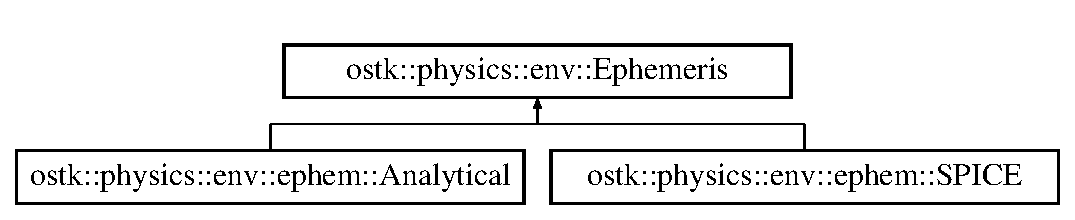
\includegraphics[height=2.000000cm]{classostk_1_1physics_1_1env_1_1_ephemeris}
\end{center}
\end{figure}
\subsection*{Public Member Functions}
\begin{DoxyCompactItemize}
\item 
\hyperlink{classostk_1_1physics_1_1env_1_1_ephemeris_a4624f9a04ae931f4b4d40ceb2c37711c}{Ephemeris} ()
\item 
virtual \hyperlink{classostk_1_1physics_1_1env_1_1_ephemeris_a13b371b20fc11505ddd9aa05db764c58}{$\sim$\+Ephemeris} ()=0
\item 
virtual \hyperlink{classostk_1_1physics_1_1env_1_1_ephemeris}{Ephemeris} $\ast$ \hyperlink{classostk_1_1physics_1_1env_1_1_ephemeris_a3a35daaff1359882ae16b69ab6e399f6}{clone} () const =0
\item 
virtual bool \hyperlink{classostk_1_1physics_1_1env_1_1_ephemeris_ace5a637a5f25f700dfe1a2cef2b08162}{is\+Defined} () const =0
\item 
virtual Shared$<$ const \hyperlink{classostk_1_1physics_1_1coord_1_1_frame}{Frame} $>$ \hyperlink{classostk_1_1physics_1_1env_1_1_ephemeris_a7a2e78c90901d813311d51d66fcf12bf}{access\+Frame} () const =0
\end{DoxyCompactItemize}


\subsection{Detailed Description}
https\+://en.wikipedia.\+org/wiki/\+Fundamental\+\_\+ephemeris 

\subsection{Constructor \& Destructor Documentation}
\mbox{\Hypertarget{classostk_1_1physics_1_1env_1_1_ephemeris_a4624f9a04ae931f4b4d40ceb2c37711c}\label{classostk_1_1physics_1_1env_1_1_ephemeris_a4624f9a04ae931f4b4d40ceb2c37711c}} 
\index{ostk\+::physics\+::env\+::\+Ephemeris@{ostk\+::physics\+::env\+::\+Ephemeris}!Ephemeris@{Ephemeris}}
\index{Ephemeris@{Ephemeris}!ostk\+::physics\+::env\+::\+Ephemeris@{ostk\+::physics\+::env\+::\+Ephemeris}}
\subsubsection{\texorpdfstring{Ephemeris()}{Ephemeris()}}
{\footnotesize\ttfamily ostk\+::physics\+::env\+::\+Ephemeris\+::\+Ephemeris (\begin{DoxyParamCaption}{ }\end{DoxyParamCaption})}

\mbox{\Hypertarget{classostk_1_1physics_1_1env_1_1_ephemeris_a13b371b20fc11505ddd9aa05db764c58}\label{classostk_1_1physics_1_1env_1_1_ephemeris_a13b371b20fc11505ddd9aa05db764c58}} 
\index{ostk\+::physics\+::env\+::\+Ephemeris@{ostk\+::physics\+::env\+::\+Ephemeris}!````~Ephemeris@{$\sim$\+Ephemeris}}
\index{````~Ephemeris@{$\sim$\+Ephemeris}!ostk\+::physics\+::env\+::\+Ephemeris@{ostk\+::physics\+::env\+::\+Ephemeris}}
\subsubsection{\texorpdfstring{$\sim$\+Ephemeris()}{~Ephemeris()}}
{\footnotesize\ttfamily ostk\+::physics\+::env\+::\+Ephemeris\+::$\sim$\+Ephemeris (\begin{DoxyParamCaption}{ }\end{DoxyParamCaption})\hspace{0.3cm}{\ttfamily [pure virtual]}}



\subsection{Member Function Documentation}
\mbox{\Hypertarget{classostk_1_1physics_1_1env_1_1_ephemeris_a7a2e78c90901d813311d51d66fcf12bf}\label{classostk_1_1physics_1_1env_1_1_ephemeris_a7a2e78c90901d813311d51d66fcf12bf}} 
\index{ostk\+::physics\+::env\+::\+Ephemeris@{ostk\+::physics\+::env\+::\+Ephemeris}!access\+Frame@{access\+Frame}}
\index{access\+Frame@{access\+Frame}!ostk\+::physics\+::env\+::\+Ephemeris@{ostk\+::physics\+::env\+::\+Ephemeris}}
\subsubsection{\texorpdfstring{access\+Frame()}{accessFrame()}}
{\footnotesize\ttfamily virtual Shared$<$const \hyperlink{classostk_1_1physics_1_1coord_1_1_frame}{Frame}$>$ ostk\+::physics\+::env\+::\+Ephemeris\+::access\+Frame (\begin{DoxyParamCaption}{ }\end{DoxyParamCaption}) const\hspace{0.3cm}{\ttfamily [pure virtual]}}



Implemented in \hyperlink{classostk_1_1physics_1_1env_1_1ephem_1_1_s_p_i_c_e_abf9dee32d47dbb1308af0c9783c84854}{ostk\+::physics\+::env\+::ephem\+::\+S\+P\+I\+CE}, and \hyperlink{classostk_1_1physics_1_1env_1_1ephem_1_1_analytical_a380712abe920ca25b2a3526d4a776033}{ostk\+::physics\+::env\+::ephem\+::\+Analytical}.

\mbox{\Hypertarget{classostk_1_1physics_1_1env_1_1_ephemeris_a3a35daaff1359882ae16b69ab6e399f6}\label{classostk_1_1physics_1_1env_1_1_ephemeris_a3a35daaff1359882ae16b69ab6e399f6}} 
\index{ostk\+::physics\+::env\+::\+Ephemeris@{ostk\+::physics\+::env\+::\+Ephemeris}!clone@{clone}}
\index{clone@{clone}!ostk\+::physics\+::env\+::\+Ephemeris@{ostk\+::physics\+::env\+::\+Ephemeris}}
\subsubsection{\texorpdfstring{clone()}{clone()}}
{\footnotesize\ttfamily virtual \hyperlink{classostk_1_1physics_1_1env_1_1_ephemeris}{Ephemeris}$\ast$ ostk\+::physics\+::env\+::\+Ephemeris\+::clone (\begin{DoxyParamCaption}{ }\end{DoxyParamCaption}) const\hspace{0.3cm}{\ttfamily [pure virtual]}}



Implemented in \hyperlink{classostk_1_1physics_1_1env_1_1ephem_1_1_s_p_i_c_e_af9155765c2546bd8707b56ed86f77c2d}{ostk\+::physics\+::env\+::ephem\+::\+S\+P\+I\+CE}, and \hyperlink{classostk_1_1physics_1_1env_1_1ephem_1_1_analytical_aeb01e31d1fd2d142efa5815ff3a44ea4}{ostk\+::physics\+::env\+::ephem\+::\+Analytical}.

\mbox{\Hypertarget{classostk_1_1physics_1_1env_1_1_ephemeris_ace5a637a5f25f700dfe1a2cef2b08162}\label{classostk_1_1physics_1_1env_1_1_ephemeris_ace5a637a5f25f700dfe1a2cef2b08162}} 
\index{ostk\+::physics\+::env\+::\+Ephemeris@{ostk\+::physics\+::env\+::\+Ephemeris}!is\+Defined@{is\+Defined}}
\index{is\+Defined@{is\+Defined}!ostk\+::physics\+::env\+::\+Ephemeris@{ostk\+::physics\+::env\+::\+Ephemeris}}
\subsubsection{\texorpdfstring{is\+Defined()}{isDefined()}}
{\footnotesize\ttfamily virtual bool ostk\+::physics\+::env\+::\+Ephemeris\+::is\+Defined (\begin{DoxyParamCaption}{ }\end{DoxyParamCaption}) const\hspace{0.3cm}{\ttfamily [pure virtual]}}



Implemented in \hyperlink{classostk_1_1physics_1_1env_1_1ephem_1_1_s_p_i_c_e_a2e5350a46c5efe938998b760ee783f77}{ostk\+::physics\+::env\+::ephem\+::\+S\+P\+I\+CE}, and \hyperlink{classostk_1_1physics_1_1env_1_1ephem_1_1_analytical_ac832a4552abfbeba38891cb936bc15ef}{ostk\+::physics\+::env\+::ephem\+::\+Analytical}.



The documentation for this class was generated from the following files\+:\begin{DoxyCompactItemize}
\item 
include/\+Open\+Space\+Toolkit/\+Physics/\+Environment/\hyperlink{_ephemeris_8hpp}{Ephemeris.\+hpp}\item 
src/\+Open\+Space\+Toolkit/\+Physics/\+Environment/\hyperlink{_ephemeris_8cpp}{Ephemeris.\+cpp}\end{DoxyCompactItemize}

\hypertarget{classostk_1_1physics_1_1coord_1_1frame_1_1provider_1_1iers_1_1_finals2000_a}{}\section{ostk\+:\+:physics\+:\+:coord\+:\+:frame\+:\+:provider\+:\+:iers\+:\+:Finals2000A Class Reference}
\label{classostk_1_1physics_1_1coord_1_1frame_1_1provider_1_1iers_1_1_finals2000_a}\index{ostk\+::physics\+::coord\+::frame\+::provider\+::iers\+::\+Finals2000A@{ostk\+::physics\+::coord\+::frame\+::provider\+::iers\+::\+Finals2000A}}


Standard Rapid E\+OP \hyperlink{structostk_1_1physics_1_1coord_1_1frame_1_1provider_1_1iers_1_1_finals2000_a_1_1_data}{Data} since 01. January 1992 (I\+A\+U2000)  




{\ttfamily \#include $<$Finals2000\+A.\+hpp$>$}

\subsection*{Classes}
\begin{DoxyCompactItemize}
\item 
struct \hyperlink{structostk_1_1physics_1_1coord_1_1frame_1_1provider_1_1iers_1_1_finals2000_a_1_1_data}{Data}
\end{DoxyCompactItemize}
\subsection*{Public Member Functions}
\begin{DoxyCompactItemize}
\item 
bool \hyperlink{classostk_1_1physics_1_1coord_1_1frame_1_1provider_1_1iers_1_1_finals2000_a_ac1214bb5570078e02ff8dc56bc846e9c}{is\+Defined} () const
\item 
\hyperlink{classostk_1_1physics_1_1time_1_1_interval}{Interval} \hyperlink{classostk_1_1physics_1_1coord_1_1frame_1_1provider_1_1iers_1_1_finals2000_a_a80c02efda876c2359d5f26a5804dff2d}{get\+Interval} () const
\item 
Vector2d \hyperlink{classostk_1_1physics_1_1coord_1_1frame_1_1provider_1_1iers_1_1_finals2000_a_acbe4bbe907144a93e2746b482e7d1e99}{get\+Polar\+Motion\+At} (const \hyperlink{classostk_1_1physics_1_1time_1_1_instant}{Instant} \&an\+Instant) const
\item 
Real \hyperlink{classostk_1_1physics_1_1coord_1_1frame_1_1provider_1_1iers_1_1_finals2000_a_af466fab804c2eed95804a0670e90e3dd}{get\+Ut1\+Minus\+Utc\+At} (const \hyperlink{classostk_1_1physics_1_1time_1_1_instant}{Instant} \&an\+Instant) const
\item 
Real \hyperlink{classostk_1_1physics_1_1coord_1_1frame_1_1provider_1_1iers_1_1_finals2000_a_a3c0b965e872a454f69cf7dbcf4fb61d8}{get\+Lod\+At} (const \hyperlink{classostk_1_1physics_1_1time_1_1_instant}{Instant} \&an\+Instant) const
\item 
\hyperlink{structostk_1_1physics_1_1coord_1_1frame_1_1provider_1_1iers_1_1_finals2000_a_1_1_data}{Finals2000\+A\+::\+Data} \hyperlink{classostk_1_1physics_1_1coord_1_1frame_1_1provider_1_1iers_1_1_finals2000_a_ae945e5caae2390991db7eae67ba34016}{get\+Data\+At} (const \hyperlink{classostk_1_1physics_1_1time_1_1_instant}{Instant} \&an\+Instant) const
\end{DoxyCompactItemize}
\subsection*{Static Public Member Functions}
\begin{DoxyCompactItemize}
\item 
static \hyperlink{classostk_1_1physics_1_1coord_1_1frame_1_1provider_1_1iers_1_1_finals2000_a}{Finals2000A} \hyperlink{classostk_1_1physics_1_1coord_1_1frame_1_1provider_1_1iers_1_1_finals2000_a_a78af6630d9b4b0cac43e41b0da25a54f}{Undefined} ()
\item 
static \hyperlink{classostk_1_1physics_1_1coord_1_1frame_1_1provider_1_1iers_1_1_finals2000_a}{Finals2000A} \hyperlink{classostk_1_1physics_1_1coord_1_1frame_1_1provider_1_1iers_1_1_finals2000_a_a914784bcc11e8eb6c2feedd288433a8f}{Load} (const fs\+::\+File \&a\+File)
\end{DoxyCompactItemize}
\subsection*{Friends}
\begin{DoxyCompactItemize}
\item 
std\+::ostream \& \hyperlink{classostk_1_1physics_1_1coord_1_1frame_1_1provider_1_1iers_1_1_finals2000_a_ade92763eb1cb719a4a499af1beb72b43}{operator$<$$<$} (std\+::ostream \&an\+Output\+Stream, const \hyperlink{classostk_1_1physics_1_1coord_1_1frame_1_1provider_1_1iers_1_1_finals2000_a}{Finals2000A} \&a\+Finals2000A)
\end{DoxyCompactItemize}


\subsection{Detailed Description}
Standard Rapid E\+OP \hyperlink{structostk_1_1physics_1_1coord_1_1frame_1_1provider_1_1iers_1_1_finals2000_a_1_1_data}{Data} since 01. January 1992 (I\+A\+U2000) 

This file (updated weekly) is the complete Earth orientation data set, since 1 January 1992 with 1 year of predictions. The nutation series in dX and dY uses the I\+AU 2000A Nutation Theory.

https\+://www.iers.\+org/\+I\+E\+R\+S/\+E\+N/\+Data\+Products/\+Earth\+Orientation\+Data/eop.html -\/$>$ finals.\+data (I\+A\+U2000) 

\subsection{Member Function Documentation}
\mbox{\Hypertarget{classostk_1_1physics_1_1coord_1_1frame_1_1provider_1_1iers_1_1_finals2000_a_ae945e5caae2390991db7eae67ba34016}\label{classostk_1_1physics_1_1coord_1_1frame_1_1provider_1_1iers_1_1_finals2000_a_ae945e5caae2390991db7eae67ba34016}} 
\index{ostk\+::physics\+::coord\+::frame\+::provider\+::iers\+::\+Finals2000A@{ostk\+::physics\+::coord\+::frame\+::provider\+::iers\+::\+Finals2000A}!get\+Data\+At@{get\+Data\+At}}
\index{get\+Data\+At@{get\+Data\+At}!ostk\+::physics\+::coord\+::frame\+::provider\+::iers\+::\+Finals2000A@{ostk\+::physics\+::coord\+::frame\+::provider\+::iers\+::\+Finals2000A}}
\subsubsection{\texorpdfstring{get\+Data\+At()}{getDataAt()}}
{\footnotesize\ttfamily \hyperlink{structostk_1_1physics_1_1coord_1_1frame_1_1provider_1_1iers_1_1_finals2000_a_1_1_data}{Finals2000\+A\+::\+Data} ostk\+::physics\+::coord\+::frame\+::provider\+::iers\+::\+Finals2000\+A\+::get\+Data\+At (\begin{DoxyParamCaption}\item[{const \hyperlink{classostk_1_1physics_1_1time_1_1_instant}{Instant} \&}]{an\+Instant }\end{DoxyParamCaption}) const}

\mbox{\Hypertarget{classostk_1_1physics_1_1coord_1_1frame_1_1provider_1_1iers_1_1_finals2000_a_a80c02efda876c2359d5f26a5804dff2d}\label{classostk_1_1physics_1_1coord_1_1frame_1_1provider_1_1iers_1_1_finals2000_a_a80c02efda876c2359d5f26a5804dff2d}} 
\index{ostk\+::physics\+::coord\+::frame\+::provider\+::iers\+::\+Finals2000A@{ostk\+::physics\+::coord\+::frame\+::provider\+::iers\+::\+Finals2000A}!get\+Interval@{get\+Interval}}
\index{get\+Interval@{get\+Interval}!ostk\+::physics\+::coord\+::frame\+::provider\+::iers\+::\+Finals2000A@{ostk\+::physics\+::coord\+::frame\+::provider\+::iers\+::\+Finals2000A}}
\subsubsection{\texorpdfstring{get\+Interval()}{getInterval()}}
{\footnotesize\ttfamily \hyperlink{classostk_1_1physics_1_1time_1_1_interval}{Interval} ostk\+::physics\+::coord\+::frame\+::provider\+::iers\+::\+Finals2000\+A\+::get\+Interval (\begin{DoxyParamCaption}{ }\end{DoxyParamCaption}) const}

\mbox{\Hypertarget{classostk_1_1physics_1_1coord_1_1frame_1_1provider_1_1iers_1_1_finals2000_a_a3c0b965e872a454f69cf7dbcf4fb61d8}\label{classostk_1_1physics_1_1coord_1_1frame_1_1provider_1_1iers_1_1_finals2000_a_a3c0b965e872a454f69cf7dbcf4fb61d8}} 
\index{ostk\+::physics\+::coord\+::frame\+::provider\+::iers\+::\+Finals2000A@{ostk\+::physics\+::coord\+::frame\+::provider\+::iers\+::\+Finals2000A}!get\+Lod\+At@{get\+Lod\+At}}
\index{get\+Lod\+At@{get\+Lod\+At}!ostk\+::physics\+::coord\+::frame\+::provider\+::iers\+::\+Finals2000A@{ostk\+::physics\+::coord\+::frame\+::provider\+::iers\+::\+Finals2000A}}
\subsubsection{\texorpdfstring{get\+Lod\+At()}{getLodAt()}}
{\footnotesize\ttfamily Real ostk\+::physics\+::coord\+::frame\+::provider\+::iers\+::\+Finals2000\+A\+::get\+Lod\+At (\begin{DoxyParamCaption}\item[{const \hyperlink{classostk_1_1physics_1_1time_1_1_instant}{Instant} \&}]{an\+Instant }\end{DoxyParamCaption}) const}

\mbox{\Hypertarget{classostk_1_1physics_1_1coord_1_1frame_1_1provider_1_1iers_1_1_finals2000_a_acbe4bbe907144a93e2746b482e7d1e99}\label{classostk_1_1physics_1_1coord_1_1frame_1_1provider_1_1iers_1_1_finals2000_a_acbe4bbe907144a93e2746b482e7d1e99}} 
\index{ostk\+::physics\+::coord\+::frame\+::provider\+::iers\+::\+Finals2000A@{ostk\+::physics\+::coord\+::frame\+::provider\+::iers\+::\+Finals2000A}!get\+Polar\+Motion\+At@{get\+Polar\+Motion\+At}}
\index{get\+Polar\+Motion\+At@{get\+Polar\+Motion\+At}!ostk\+::physics\+::coord\+::frame\+::provider\+::iers\+::\+Finals2000A@{ostk\+::physics\+::coord\+::frame\+::provider\+::iers\+::\+Finals2000A}}
\subsubsection{\texorpdfstring{get\+Polar\+Motion\+At()}{getPolarMotionAt()}}
{\footnotesize\ttfamily Vector2d ostk\+::physics\+::coord\+::frame\+::provider\+::iers\+::\+Finals2000\+A\+::get\+Polar\+Motion\+At (\begin{DoxyParamCaption}\item[{const \hyperlink{classostk_1_1physics_1_1time_1_1_instant}{Instant} \&}]{an\+Instant }\end{DoxyParamCaption}) const}

\mbox{\Hypertarget{classostk_1_1physics_1_1coord_1_1frame_1_1provider_1_1iers_1_1_finals2000_a_af466fab804c2eed95804a0670e90e3dd}\label{classostk_1_1physics_1_1coord_1_1frame_1_1provider_1_1iers_1_1_finals2000_a_af466fab804c2eed95804a0670e90e3dd}} 
\index{ostk\+::physics\+::coord\+::frame\+::provider\+::iers\+::\+Finals2000A@{ostk\+::physics\+::coord\+::frame\+::provider\+::iers\+::\+Finals2000A}!get\+Ut1\+Minus\+Utc\+At@{get\+Ut1\+Minus\+Utc\+At}}
\index{get\+Ut1\+Minus\+Utc\+At@{get\+Ut1\+Minus\+Utc\+At}!ostk\+::physics\+::coord\+::frame\+::provider\+::iers\+::\+Finals2000A@{ostk\+::physics\+::coord\+::frame\+::provider\+::iers\+::\+Finals2000A}}
\subsubsection{\texorpdfstring{get\+Ut1\+Minus\+Utc\+At()}{getUt1MinusUtcAt()}}
{\footnotesize\ttfamily Real ostk\+::physics\+::coord\+::frame\+::provider\+::iers\+::\+Finals2000\+A\+::get\+Ut1\+Minus\+Utc\+At (\begin{DoxyParamCaption}\item[{const \hyperlink{classostk_1_1physics_1_1time_1_1_instant}{Instant} \&}]{an\+Instant }\end{DoxyParamCaption}) const}

\mbox{\Hypertarget{classostk_1_1physics_1_1coord_1_1frame_1_1provider_1_1iers_1_1_finals2000_a_ac1214bb5570078e02ff8dc56bc846e9c}\label{classostk_1_1physics_1_1coord_1_1frame_1_1provider_1_1iers_1_1_finals2000_a_ac1214bb5570078e02ff8dc56bc846e9c}} 
\index{ostk\+::physics\+::coord\+::frame\+::provider\+::iers\+::\+Finals2000A@{ostk\+::physics\+::coord\+::frame\+::provider\+::iers\+::\+Finals2000A}!is\+Defined@{is\+Defined}}
\index{is\+Defined@{is\+Defined}!ostk\+::physics\+::coord\+::frame\+::provider\+::iers\+::\+Finals2000A@{ostk\+::physics\+::coord\+::frame\+::provider\+::iers\+::\+Finals2000A}}
\subsubsection{\texorpdfstring{is\+Defined()}{isDefined()}}
{\footnotesize\ttfamily bool ostk\+::physics\+::coord\+::frame\+::provider\+::iers\+::\+Finals2000\+A\+::is\+Defined (\begin{DoxyParamCaption}{ }\end{DoxyParamCaption}) const}

\mbox{\Hypertarget{classostk_1_1physics_1_1coord_1_1frame_1_1provider_1_1iers_1_1_finals2000_a_a914784bcc11e8eb6c2feedd288433a8f}\label{classostk_1_1physics_1_1coord_1_1frame_1_1provider_1_1iers_1_1_finals2000_a_a914784bcc11e8eb6c2feedd288433a8f}} 
\index{ostk\+::physics\+::coord\+::frame\+::provider\+::iers\+::\+Finals2000A@{ostk\+::physics\+::coord\+::frame\+::provider\+::iers\+::\+Finals2000A}!Load@{Load}}
\index{Load@{Load}!ostk\+::physics\+::coord\+::frame\+::provider\+::iers\+::\+Finals2000A@{ostk\+::physics\+::coord\+::frame\+::provider\+::iers\+::\+Finals2000A}}
\subsubsection{\texorpdfstring{Load()}{Load()}}
{\footnotesize\ttfamily \hyperlink{classostk_1_1physics_1_1coord_1_1frame_1_1provider_1_1iers_1_1_finals2000_a}{Finals2000A} ostk\+::physics\+::coord\+::frame\+::provider\+::iers\+::\+Finals2000\+A\+::\+Load (\begin{DoxyParamCaption}\item[{const fs\+::\+File \&}]{a\+File }\end{DoxyParamCaption})\hspace{0.3cm}{\ttfamily [static]}}

\mbox{\Hypertarget{classostk_1_1physics_1_1coord_1_1frame_1_1provider_1_1iers_1_1_finals2000_a_a78af6630d9b4b0cac43e41b0da25a54f}\label{classostk_1_1physics_1_1coord_1_1frame_1_1provider_1_1iers_1_1_finals2000_a_a78af6630d9b4b0cac43e41b0da25a54f}} 
\index{ostk\+::physics\+::coord\+::frame\+::provider\+::iers\+::\+Finals2000A@{ostk\+::physics\+::coord\+::frame\+::provider\+::iers\+::\+Finals2000A}!Undefined@{Undefined}}
\index{Undefined@{Undefined}!ostk\+::physics\+::coord\+::frame\+::provider\+::iers\+::\+Finals2000A@{ostk\+::physics\+::coord\+::frame\+::provider\+::iers\+::\+Finals2000A}}
\subsubsection{\texorpdfstring{Undefined()}{Undefined()}}
{\footnotesize\ttfamily \hyperlink{classostk_1_1physics_1_1coord_1_1frame_1_1provider_1_1iers_1_1_finals2000_a}{Finals2000A} ostk\+::physics\+::coord\+::frame\+::provider\+::iers\+::\+Finals2000\+A\+::\+Undefined (\begin{DoxyParamCaption}{ }\end{DoxyParamCaption})\hspace{0.3cm}{\ttfamily [static]}}



\subsection{Friends And Related Function Documentation}
\mbox{\Hypertarget{classostk_1_1physics_1_1coord_1_1frame_1_1provider_1_1iers_1_1_finals2000_a_ade92763eb1cb719a4a499af1beb72b43}\label{classostk_1_1physics_1_1coord_1_1frame_1_1provider_1_1iers_1_1_finals2000_a_ade92763eb1cb719a4a499af1beb72b43}} 
\index{ostk\+::physics\+::coord\+::frame\+::provider\+::iers\+::\+Finals2000A@{ostk\+::physics\+::coord\+::frame\+::provider\+::iers\+::\+Finals2000A}!operator$<$$<$@{operator$<$$<$}}
\index{operator$<$$<$@{operator$<$$<$}!ostk\+::physics\+::coord\+::frame\+::provider\+::iers\+::\+Finals2000A@{ostk\+::physics\+::coord\+::frame\+::provider\+::iers\+::\+Finals2000A}}
\subsubsection{\texorpdfstring{operator$<$$<$}{operator<<}}
{\footnotesize\ttfamily std\+::ostream\& operator$<$$<$ (\begin{DoxyParamCaption}\item[{std\+::ostream \&}]{an\+Output\+Stream,  }\item[{const \hyperlink{classostk_1_1physics_1_1coord_1_1frame_1_1provider_1_1iers_1_1_finals2000_a}{Finals2000A} \&}]{a\+Finals2000A }\end{DoxyParamCaption})\hspace{0.3cm}{\ttfamily [friend]}}



The documentation for this class was generated from the following files\+:\begin{DoxyCompactItemize}
\item 
include/\+Open\+Space\+Toolkit/\+Physics/\+Coordinate/\+Frame/\+Providers/\+I\+E\+R\+S/\hyperlink{_finals2000_a_8hpp}{Finals2000\+A.\+hpp}\item 
src/\+Open\+Space\+Toolkit/\+Physics/\+Coordinate/\+Frame/\+Providers/\+I\+E\+R\+S/\hyperlink{_finals2000_a_8cpp}{Finals2000\+A.\+cpp}\end{DoxyCompactItemize}

\hypertarget{classostk_1_1physics_1_1coord_1_1_frame}{}\section{ostk\+:\+:physics\+:\+:coord\+:\+:Frame Class Reference}
\label{classostk_1_1physics_1_1coord_1_1_frame}\index{ostk\+::physics\+::coord\+::\+Frame@{ostk\+::physics\+::coord\+::\+Frame}}


Reference frame.  




{\ttfamily \#include $<$Frame.\+hpp$>$}

Inheritance diagram for ostk\+:\+:physics\+:\+:coord\+:\+:Frame\+:\begin{figure}[H]
\begin{center}
\leavevmode
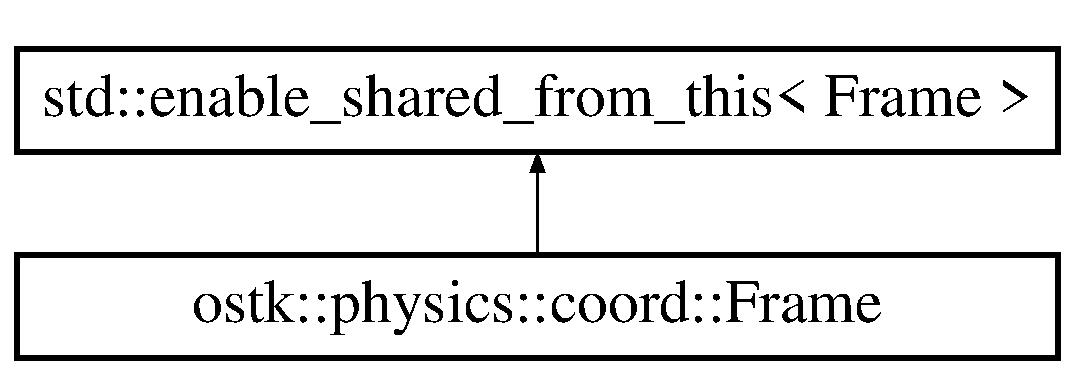
\includegraphics[height=2.000000cm]{classostk_1_1physics_1_1coord_1_1_frame}
\end{center}
\end{figure}
\subsection*{Public Member Functions}
\begin{DoxyCompactItemize}
\item 
\hyperlink{classostk_1_1physics_1_1coord_1_1_frame_a9c8b5b7869ee8e730e0b23be60920a9d}{$\sim$\+Frame} ()
\begin{DoxyCompactList}\small\item\em Destructor. \end{DoxyCompactList}\item 
bool \hyperlink{classostk_1_1physics_1_1coord_1_1_frame_a010fbd30fe3a937d44d0fbbdeb60222b}{operator==} (const \hyperlink{classostk_1_1physics_1_1coord_1_1_frame}{Frame} \&a\+Frame) const
\item 
bool \hyperlink{classostk_1_1physics_1_1coord_1_1_frame_a12a5cb341c34a404f220b0940a5dff79}{operator!=} (const \hyperlink{classostk_1_1physics_1_1coord_1_1_frame}{Frame} \&a\+Frame) const
\item 
bool \hyperlink{classostk_1_1physics_1_1coord_1_1_frame_a3c4750cec74616ad3e48adf31c314756}{is\+Defined} () const
\item 
bool \hyperlink{classostk_1_1physics_1_1coord_1_1_frame_ac0f7d78be14f09ccef5b862c4f963da8}{is\+Quasi\+Inertial} () const
\item 
bool \hyperlink{classostk_1_1physics_1_1coord_1_1_frame_aa4c778fa91e6599cdea0a889fd5bf69c}{has\+Parent} () const
\item 
Shared$<$ const \hyperlink{classostk_1_1physics_1_1coord_1_1_frame}{Frame} $>$ \hyperlink{classostk_1_1physics_1_1coord_1_1_frame_a549b54435e1a47193ff7288df9d2b0cb}{access\+Parent} () const
\item 
Shared$<$ const \hyperlink{classostk_1_1physics_1_1coord_1_1_frame}{Frame} $>$ \hyperlink{classostk_1_1physics_1_1coord_1_1_frame_af2276e1ed3a74752194ae3414b10636d}{access\+Ancestor} (const Uint8 an\+Ancestor\+Degree) const
\item 
Shared$<$ const \hyperlink{classostk_1_1physics_1_1coord_1_1frame_1_1_provider}{Provider} $>$ \hyperlink{classostk_1_1physics_1_1coord_1_1_frame_a60c1717e04993577c0dcf4eae23be672}{access\+Provider} () const
\item 
String \hyperlink{classostk_1_1physics_1_1coord_1_1_frame_a47aca195a73e14198f6d615c8988ce6e}{get\+Name} () const
\item 
\hyperlink{classostk_1_1physics_1_1coord_1_1_position}{Position} \hyperlink{classostk_1_1physics_1_1coord_1_1_frame_a9f0544fd284d2ff4bca6a54dc8835bff}{get\+Origin\+In} (const Shared$<$ const \hyperlink{classostk_1_1physics_1_1coord_1_1_frame}{Frame} $>$ \&a\+Frame, const \hyperlink{classostk_1_1physics_1_1time_1_1_instant}{Instant} \&an\+Instant) const
\item 
\hyperlink{classostk_1_1physics_1_1coord_1_1_velocity}{Velocity} \hyperlink{classostk_1_1physics_1_1coord_1_1_frame_ab2d8bdcd3f68604d4ca104341f51b7f1}{get\+Velocity\+In} (const Shared$<$ const \hyperlink{classostk_1_1physics_1_1coord_1_1_frame}{Frame} $>$ \&a\+Frame, const \hyperlink{classostk_1_1physics_1_1time_1_1_instant}{Instant} \&an\+Instant) const
\item 
\hyperlink{classostk_1_1physics_1_1coord_1_1_axes}{Axes} \hyperlink{classostk_1_1physics_1_1coord_1_1_frame_ac75780963694dd74ea2e6a66f6ae17d8}{get\+Axes\+In} (const Shared$<$ const \hyperlink{classostk_1_1physics_1_1coord_1_1_frame}{Frame} $>$ \&a\+Frame, const \hyperlink{classostk_1_1physics_1_1time_1_1_instant}{Instant} \&an\+Instant) const
\item 
\hyperlink{classostk_1_1physics_1_1coord_1_1_transform}{Transform} \hyperlink{classostk_1_1physics_1_1coord_1_1_frame_aa6f51c81724f36644ad8343a1124c264}{get\+Transform\+To} (const Shared$<$ const \hyperlink{classostk_1_1physics_1_1coord_1_1_frame}{Frame} $>$ \&a\+Frame, const \hyperlink{classostk_1_1physics_1_1time_1_1_instant}{Instant} \&an\+Instant) const
\end{DoxyCompactItemize}
\subsection*{Static Public Member Functions}
\begin{DoxyCompactItemize}
\item 
static Shared$<$ const \hyperlink{classostk_1_1physics_1_1coord_1_1_frame}{Frame} $>$ \hyperlink{classostk_1_1physics_1_1coord_1_1_frame_a292d32b849648a8e530d35ac47b5c699}{Undefined} ()
\item 
static Shared$<$ const \hyperlink{classostk_1_1physics_1_1coord_1_1_frame}{Frame} $>$ \hyperlink{classostk_1_1physics_1_1coord_1_1_frame_af111d96da6adf5405a354a769618b5f4}{I\+C\+RF} ()
\item 
static Shared$<$ const \hyperlink{classostk_1_1physics_1_1coord_1_1_frame}{Frame} $>$ \hyperlink{classostk_1_1physics_1_1coord_1_1_frame_abe31c60e3e7f654b101876cb6b9b5238}{G\+C\+RF} ()
\item 
static Shared$<$ const \hyperlink{classostk_1_1physics_1_1coord_1_1_frame}{Frame} $>$ \hyperlink{classostk_1_1physics_1_1coord_1_1_frame_a61b7c68b761966956251d393bf57f5e5}{E\+M\+E2000} ()
\item 
static Shared$<$ const \hyperlink{classostk_1_1physics_1_1coord_1_1_frame}{Frame} $>$ \hyperlink{classostk_1_1physics_1_1coord_1_1_frame_a1441cef9cd2abe312753f3a81606adfb}{T\+E\+ME} ()
\item 
static Shared$<$ const \hyperlink{classostk_1_1physics_1_1coord_1_1_frame}{Frame} $>$ \hyperlink{classostk_1_1physics_1_1coord_1_1_frame_ab47046bc517b04537c96844d95c13fdd}{T\+E\+M\+E\+Of\+Epoch} (const \hyperlink{classostk_1_1physics_1_1time_1_1_instant}{Instant} \&an\+Epoch)
\item 
static Shared$<$ const \hyperlink{classostk_1_1physics_1_1coord_1_1_frame}{Frame} $>$ \hyperlink{classostk_1_1physics_1_1coord_1_1_frame_ae858400dfa432f12b71712b52b3f5108}{C\+I\+RF} ()
\item 
static Shared$<$ const \hyperlink{classostk_1_1physics_1_1coord_1_1_frame}{Frame} $>$ \hyperlink{classostk_1_1physics_1_1coord_1_1_frame_ac159b1d21bc5f55e7163d27f4cc25c34}{T\+I\+RF} ()
\item 
static Shared$<$ const \hyperlink{classostk_1_1physics_1_1coord_1_1_frame}{Frame} $>$ \hyperlink{classostk_1_1physics_1_1coord_1_1_frame_ac1d0d50dc15982fbef3caba62a9ed507}{I\+T\+RF} ()
\item 
static Shared$<$ const \hyperlink{classostk_1_1physics_1_1coord_1_1_frame}{Frame} $>$ \hyperlink{classostk_1_1physics_1_1coord_1_1_frame_ad9f12f000a68daaec4969ba739f43ee7}{With\+Name} (const String \&a\+Name)
\item 
static bool \hyperlink{classostk_1_1physics_1_1coord_1_1_frame_afe14b695035c704b408563a12a47eb38}{Exists} (const String \&a\+Name)
\item 
static Shared$<$ const \hyperlink{classostk_1_1physics_1_1coord_1_1_frame}{Frame} $>$ \hyperlink{classostk_1_1physics_1_1coord_1_1_frame_a6faa8908c55e5e56ce3ed4c96d15b9af}{Construct} (const String \&a\+Name, bool \hyperlink{classostk_1_1physics_1_1coord_1_1_frame_ac0f7d78be14f09ccef5b862c4f963da8}{is\+Quasi\+Inertial}, const Shared$<$ const \hyperlink{classostk_1_1physics_1_1coord_1_1_frame}{Frame} $>$ \&a\+Parent\+Frame, const Shared$<$ const \hyperlink{classostk_1_1physics_1_1coord_1_1frame_1_1_provider}{Provider} $>$ \&a\+Provider)
\begin{DoxyCompactList}\small\item\em Constructor. \end{DoxyCompactList}\item 
static void \hyperlink{classostk_1_1physics_1_1coord_1_1_frame_a2c4bf16207b59862deaeee224153b8f9}{Destruct} (const String \&a\+Name)
\end{DoxyCompactItemize}
\subsection*{Protected Member Functions}
\begin{DoxyCompactItemize}
\item 
\hyperlink{classostk_1_1physics_1_1coord_1_1_frame_a66f32d0c9dd2497b6e7ace4fcccbce60}{Frame} (const String \&a\+Name, bool \hyperlink{classostk_1_1physics_1_1coord_1_1_frame_ac0f7d78be14f09ccef5b862c4f963da8}{is\+Quasi\+Inertial}, const Shared$<$ const \hyperlink{classostk_1_1physics_1_1coord_1_1_frame}{Frame} $>$ \&a\+Parent\+Frame, const Shared$<$ const \hyperlink{classostk_1_1physics_1_1coord_1_1frame_1_1_provider}{Provider} $>$ \&a\+Provider)
\item 
\hyperlink{classostk_1_1physics_1_1coord_1_1_frame_acaa7ddfcad1566838ca72bf431a3bd4f}{Frame} (const \hyperlink{classostk_1_1physics_1_1coord_1_1_frame}{Frame} \&a\+Frame)=default
\item 
\hyperlink{classostk_1_1physics_1_1coord_1_1_frame}{Frame} \& \hyperlink{classostk_1_1physics_1_1coord_1_1_frame_ac47e4fe942c8cd0b8969ee9f6d32b816}{operator=} (const \hyperlink{classostk_1_1physics_1_1coord_1_1_frame}{Frame} \&a\+Frame)=default
\end{DoxyCompactItemize}
\subsection*{Friends}
\begin{DoxyCompactItemize}
\item 
std\+::ostream \& \hyperlink{classostk_1_1physics_1_1coord_1_1_frame_a509ac1926cfc3553748bace204e2b1cc}{operator$<$$<$} (std\+::ostream \&an\+Output\+Stream, const \hyperlink{classostk_1_1physics_1_1coord_1_1_frame}{Frame} \&a\+Frame)
\end{DoxyCompactItemize}


\subsection{Detailed Description}
Reference frame. 

https\+://en.wikipedia.\+org/wiki/\+Frame\+\_\+of\+\_\+reference \begin{DoxyNote}{Note}
Implementation heavily inspired by (the great!) \href{https://www.orekit.org/static/architecture/frames.html}{\tt https\+://www.\+orekit.\+org/static/architecture/frames.\+html} 
\end{DoxyNote}


\subsection{Constructor \& Destructor Documentation}
\mbox{\Hypertarget{classostk_1_1physics_1_1coord_1_1_frame_a9c8b5b7869ee8e730e0b23be60920a9d}\label{classostk_1_1physics_1_1coord_1_1_frame_a9c8b5b7869ee8e730e0b23be60920a9d}} 
\index{ostk\+::physics\+::coord\+::\+Frame@{ostk\+::physics\+::coord\+::\+Frame}!````~Frame@{$\sim$\+Frame}}
\index{````~Frame@{$\sim$\+Frame}!ostk\+::physics\+::coord\+::\+Frame@{ostk\+::physics\+::coord\+::\+Frame}}
\subsubsection{\texorpdfstring{$\sim$\+Frame()}{~Frame()}}
{\footnotesize\ttfamily ostk\+::physics\+::coord\+::\+Frame\+::$\sim$\+Frame (\begin{DoxyParamCaption}{ }\end{DoxyParamCaption})}



Destructor. 

\mbox{\Hypertarget{classostk_1_1physics_1_1coord_1_1_frame_a66f32d0c9dd2497b6e7ace4fcccbce60}\label{classostk_1_1physics_1_1coord_1_1_frame_a66f32d0c9dd2497b6e7ace4fcccbce60}} 
\index{ostk\+::physics\+::coord\+::\+Frame@{ostk\+::physics\+::coord\+::\+Frame}!Frame@{Frame}}
\index{Frame@{Frame}!ostk\+::physics\+::coord\+::\+Frame@{ostk\+::physics\+::coord\+::\+Frame}}
\subsubsection{\texorpdfstring{Frame()}{Frame()}\hspace{0.1cm}{\footnotesize\ttfamily [1/2]}}
{\footnotesize\ttfamily ostk\+::physics\+::coord\+::\+Frame\+::\+Frame (\begin{DoxyParamCaption}\item[{const String \&}]{a\+Name,  }\item[{bool}]{is\+Quasi\+Inertial,  }\item[{const Shared$<$ const \hyperlink{classostk_1_1physics_1_1coord_1_1_frame}{Frame} $>$ \&}]{a\+Parent\+Frame,  }\item[{const Shared$<$ const \hyperlink{classostk_1_1physics_1_1coord_1_1frame_1_1_provider}{Provider} $>$ \&}]{a\+Provider }\end{DoxyParamCaption})\hspace{0.3cm}{\ttfamily [protected]}}

\mbox{\Hypertarget{classostk_1_1physics_1_1coord_1_1_frame_acaa7ddfcad1566838ca72bf431a3bd4f}\label{classostk_1_1physics_1_1coord_1_1_frame_acaa7ddfcad1566838ca72bf431a3bd4f}} 
\index{ostk\+::physics\+::coord\+::\+Frame@{ostk\+::physics\+::coord\+::\+Frame}!Frame@{Frame}}
\index{Frame@{Frame}!ostk\+::physics\+::coord\+::\+Frame@{ostk\+::physics\+::coord\+::\+Frame}}
\subsubsection{\texorpdfstring{Frame()}{Frame()}\hspace{0.1cm}{\footnotesize\ttfamily [2/2]}}
{\footnotesize\ttfamily ostk\+::physics\+::coord\+::\+Frame\+::\+Frame (\begin{DoxyParamCaption}\item[{const \hyperlink{classostk_1_1physics_1_1coord_1_1_frame}{Frame} \&}]{a\+Frame }\end{DoxyParamCaption})\hspace{0.3cm}{\ttfamily [protected]}, {\ttfamily [default]}}



\subsection{Member Function Documentation}
\mbox{\Hypertarget{classostk_1_1physics_1_1coord_1_1_frame_af2276e1ed3a74752194ae3414b10636d}\label{classostk_1_1physics_1_1coord_1_1_frame_af2276e1ed3a74752194ae3414b10636d}} 
\index{ostk\+::physics\+::coord\+::\+Frame@{ostk\+::physics\+::coord\+::\+Frame}!access\+Ancestor@{access\+Ancestor}}
\index{access\+Ancestor@{access\+Ancestor}!ostk\+::physics\+::coord\+::\+Frame@{ostk\+::physics\+::coord\+::\+Frame}}
\subsubsection{\texorpdfstring{access\+Ancestor()}{accessAncestor()}}
{\footnotesize\ttfamily Shared$<$ const \hyperlink{classostk_1_1physics_1_1coord_1_1_frame}{Frame} $>$ ostk\+::physics\+::coord\+::\+Frame\+::access\+Ancestor (\begin{DoxyParamCaption}\item[{const Uint8}]{an\+Ancestor\+Degree }\end{DoxyParamCaption}) const}

\mbox{\Hypertarget{classostk_1_1physics_1_1coord_1_1_frame_a549b54435e1a47193ff7288df9d2b0cb}\label{classostk_1_1physics_1_1coord_1_1_frame_a549b54435e1a47193ff7288df9d2b0cb}} 
\index{ostk\+::physics\+::coord\+::\+Frame@{ostk\+::physics\+::coord\+::\+Frame}!access\+Parent@{access\+Parent}}
\index{access\+Parent@{access\+Parent}!ostk\+::physics\+::coord\+::\+Frame@{ostk\+::physics\+::coord\+::\+Frame}}
\subsubsection{\texorpdfstring{access\+Parent()}{accessParent()}}
{\footnotesize\ttfamily Shared$<$ const \hyperlink{classostk_1_1physics_1_1coord_1_1_frame}{Frame} $>$ ostk\+::physics\+::coord\+::\+Frame\+::access\+Parent (\begin{DoxyParamCaption}{ }\end{DoxyParamCaption}) const}

\mbox{\Hypertarget{classostk_1_1physics_1_1coord_1_1_frame_a60c1717e04993577c0dcf4eae23be672}\label{classostk_1_1physics_1_1coord_1_1_frame_a60c1717e04993577c0dcf4eae23be672}} 
\index{ostk\+::physics\+::coord\+::\+Frame@{ostk\+::physics\+::coord\+::\+Frame}!access\+Provider@{access\+Provider}}
\index{access\+Provider@{access\+Provider}!ostk\+::physics\+::coord\+::\+Frame@{ostk\+::physics\+::coord\+::\+Frame}}
\subsubsection{\texorpdfstring{access\+Provider()}{accessProvider()}}
{\footnotesize\ttfamily Shared$<$ const \hyperlink{classostk_1_1physics_1_1coord_1_1frame_1_1_provider}{Provider} $>$ ostk\+::physics\+::coord\+::\+Frame\+::access\+Provider (\begin{DoxyParamCaption}{ }\end{DoxyParamCaption}) const}

\mbox{\Hypertarget{classostk_1_1physics_1_1coord_1_1_frame_ae858400dfa432f12b71712b52b3f5108}\label{classostk_1_1physics_1_1coord_1_1_frame_ae858400dfa432f12b71712b52b3f5108}} 
\index{ostk\+::physics\+::coord\+::\+Frame@{ostk\+::physics\+::coord\+::\+Frame}!C\+I\+RF@{C\+I\+RF}}
\index{C\+I\+RF@{C\+I\+RF}!ostk\+::physics\+::coord\+::\+Frame@{ostk\+::physics\+::coord\+::\+Frame}}
\subsubsection{\texorpdfstring{C\+I\+R\+F()}{CIRF()}}
{\footnotesize\ttfamily Shared$<$ const \hyperlink{classostk_1_1physics_1_1coord_1_1_frame}{Frame} $>$ ostk\+::physics\+::coord\+::\+Frame\+::\+C\+I\+RF (\begin{DoxyParamCaption}{ }\end{DoxyParamCaption})\hspace{0.3cm}{\ttfamily [static]}}

\mbox{\Hypertarget{classostk_1_1physics_1_1coord_1_1_frame_a6faa8908c55e5e56ce3ed4c96d15b9af}\label{classostk_1_1physics_1_1coord_1_1_frame_a6faa8908c55e5e56ce3ed4c96d15b9af}} 
\index{ostk\+::physics\+::coord\+::\+Frame@{ostk\+::physics\+::coord\+::\+Frame}!Construct@{Construct}}
\index{Construct@{Construct}!ostk\+::physics\+::coord\+::\+Frame@{ostk\+::physics\+::coord\+::\+Frame}}
\subsubsection{\texorpdfstring{Construct()}{Construct()}}
{\footnotesize\ttfamily Shared$<$ const \hyperlink{classostk_1_1physics_1_1coord_1_1_frame}{Frame} $>$ ostk\+::physics\+::coord\+::\+Frame\+::\+Construct (\begin{DoxyParamCaption}\item[{const String \&}]{a\+Name,  }\item[{bool}]{is\+Quasi\+Inertial,  }\item[{const Shared$<$ const \hyperlink{classostk_1_1physics_1_1coord_1_1_frame}{Frame} $>$ \&}]{a\+Parent\+Frame,  }\item[{const Shared$<$ const \hyperlink{classostk_1_1physics_1_1coord_1_1frame_1_1_provider}{Provider} $>$ \&}]{a\+Provider }\end{DoxyParamCaption})\hspace{0.3cm}{\ttfamily [static]}}



Constructor. 


\begin{DoxyParams}[1]{Parameters}
\mbox{\tt in}  & {\em a\+Name} & A frame name \\
\hline
\mbox{\tt in}  & {\em is\+Quasi\+InertialT} & True is frame is quasi-\/inertial \\
\hline
\mbox{\tt in}  & {\em a\+Parent\+Frame} & A shared pointer to the parent frame \\
\hline
\mbox{\tt in}  & {\em a\+Provider} & A shared pointer to the transform provider \\
\hline
\end{DoxyParams}
\mbox{\Hypertarget{classostk_1_1physics_1_1coord_1_1_frame_a2c4bf16207b59862deaeee224153b8f9}\label{classostk_1_1physics_1_1coord_1_1_frame_a2c4bf16207b59862deaeee224153b8f9}} 
\index{ostk\+::physics\+::coord\+::\+Frame@{ostk\+::physics\+::coord\+::\+Frame}!Destruct@{Destruct}}
\index{Destruct@{Destruct}!ostk\+::physics\+::coord\+::\+Frame@{ostk\+::physics\+::coord\+::\+Frame}}
\subsubsection{\texorpdfstring{Destruct()}{Destruct()}}
{\footnotesize\ttfamily void ostk\+::physics\+::coord\+::\+Frame\+::\+Destruct (\begin{DoxyParamCaption}\item[{const String \&}]{a\+Name }\end{DoxyParamCaption})\hspace{0.3cm}{\ttfamily [static]}}

\mbox{\Hypertarget{classostk_1_1physics_1_1coord_1_1_frame_a61b7c68b761966956251d393bf57f5e5}\label{classostk_1_1physics_1_1coord_1_1_frame_a61b7c68b761966956251d393bf57f5e5}} 
\index{ostk\+::physics\+::coord\+::\+Frame@{ostk\+::physics\+::coord\+::\+Frame}!E\+M\+E2000@{E\+M\+E2000}}
\index{E\+M\+E2000@{E\+M\+E2000}!ostk\+::physics\+::coord\+::\+Frame@{ostk\+::physics\+::coord\+::\+Frame}}
\subsubsection{\texorpdfstring{E\+M\+E2000()}{EME2000()}}
{\footnotesize\ttfamily static Shared$<$const \hyperlink{classostk_1_1physics_1_1coord_1_1_frame}{Frame}$>$ ostk\+::physics\+::coord\+::\+Frame\+::\+E\+M\+E2000 (\begin{DoxyParamCaption}{ }\end{DoxyParamCaption})\hspace{0.3cm}{\ttfamily [static]}}

\mbox{\Hypertarget{classostk_1_1physics_1_1coord_1_1_frame_afe14b695035c704b408563a12a47eb38}\label{classostk_1_1physics_1_1coord_1_1_frame_afe14b695035c704b408563a12a47eb38}} 
\index{ostk\+::physics\+::coord\+::\+Frame@{ostk\+::physics\+::coord\+::\+Frame}!Exists@{Exists}}
\index{Exists@{Exists}!ostk\+::physics\+::coord\+::\+Frame@{ostk\+::physics\+::coord\+::\+Frame}}
\subsubsection{\texorpdfstring{Exists()}{Exists()}}
{\footnotesize\ttfamily bool ostk\+::physics\+::coord\+::\+Frame\+::\+Exists (\begin{DoxyParamCaption}\item[{const String \&}]{a\+Name }\end{DoxyParamCaption})\hspace{0.3cm}{\ttfamily [static]}}

\mbox{\Hypertarget{classostk_1_1physics_1_1coord_1_1_frame_abe31c60e3e7f654b101876cb6b9b5238}\label{classostk_1_1physics_1_1coord_1_1_frame_abe31c60e3e7f654b101876cb6b9b5238}} 
\index{ostk\+::physics\+::coord\+::\+Frame@{ostk\+::physics\+::coord\+::\+Frame}!G\+C\+RF@{G\+C\+RF}}
\index{G\+C\+RF@{G\+C\+RF}!ostk\+::physics\+::coord\+::\+Frame@{ostk\+::physics\+::coord\+::\+Frame}}
\subsubsection{\texorpdfstring{G\+C\+R\+F()}{GCRF()}}
{\footnotesize\ttfamily Shared$<$ const \hyperlink{classostk_1_1physics_1_1coord_1_1_frame}{Frame} $>$ ostk\+::physics\+::coord\+::\+Frame\+::\+G\+C\+RF (\begin{DoxyParamCaption}{ }\end{DoxyParamCaption})\hspace{0.3cm}{\ttfamily [static]}}

\mbox{\Hypertarget{classostk_1_1physics_1_1coord_1_1_frame_ac75780963694dd74ea2e6a66f6ae17d8}\label{classostk_1_1physics_1_1coord_1_1_frame_ac75780963694dd74ea2e6a66f6ae17d8}} 
\index{ostk\+::physics\+::coord\+::\+Frame@{ostk\+::physics\+::coord\+::\+Frame}!get\+Axes\+In@{get\+Axes\+In}}
\index{get\+Axes\+In@{get\+Axes\+In}!ostk\+::physics\+::coord\+::\+Frame@{ostk\+::physics\+::coord\+::\+Frame}}
\subsubsection{\texorpdfstring{get\+Axes\+In()}{getAxesIn()}}
{\footnotesize\ttfamily \hyperlink{classostk_1_1physics_1_1coord_1_1_axes}{Axes} ostk\+::physics\+::coord\+::\+Frame\+::get\+Axes\+In (\begin{DoxyParamCaption}\item[{const Shared$<$ const \hyperlink{classostk_1_1physics_1_1coord_1_1_frame}{Frame} $>$ \&}]{a\+Frame,  }\item[{const \hyperlink{classostk_1_1physics_1_1time_1_1_instant}{Instant} \&}]{an\+Instant }\end{DoxyParamCaption}) const}

\mbox{\Hypertarget{classostk_1_1physics_1_1coord_1_1_frame_a47aca195a73e14198f6d615c8988ce6e}\label{classostk_1_1physics_1_1coord_1_1_frame_a47aca195a73e14198f6d615c8988ce6e}} 
\index{ostk\+::physics\+::coord\+::\+Frame@{ostk\+::physics\+::coord\+::\+Frame}!get\+Name@{get\+Name}}
\index{get\+Name@{get\+Name}!ostk\+::physics\+::coord\+::\+Frame@{ostk\+::physics\+::coord\+::\+Frame}}
\subsubsection{\texorpdfstring{get\+Name()}{getName()}}
{\footnotesize\ttfamily String ostk\+::physics\+::coord\+::\+Frame\+::get\+Name (\begin{DoxyParamCaption}{ }\end{DoxyParamCaption}) const}

\mbox{\Hypertarget{classostk_1_1physics_1_1coord_1_1_frame_a9f0544fd284d2ff4bca6a54dc8835bff}\label{classostk_1_1physics_1_1coord_1_1_frame_a9f0544fd284d2ff4bca6a54dc8835bff}} 
\index{ostk\+::physics\+::coord\+::\+Frame@{ostk\+::physics\+::coord\+::\+Frame}!get\+Origin\+In@{get\+Origin\+In}}
\index{get\+Origin\+In@{get\+Origin\+In}!ostk\+::physics\+::coord\+::\+Frame@{ostk\+::physics\+::coord\+::\+Frame}}
\subsubsection{\texorpdfstring{get\+Origin\+In()}{getOriginIn()}}
{\footnotesize\ttfamily \hyperlink{classostk_1_1physics_1_1coord_1_1_position}{Position} ostk\+::physics\+::coord\+::\+Frame\+::get\+Origin\+In (\begin{DoxyParamCaption}\item[{const Shared$<$ const \hyperlink{classostk_1_1physics_1_1coord_1_1_frame}{Frame} $>$ \&}]{a\+Frame,  }\item[{const \hyperlink{classostk_1_1physics_1_1time_1_1_instant}{Instant} \&}]{an\+Instant }\end{DoxyParamCaption}) const}

\mbox{\Hypertarget{classostk_1_1physics_1_1coord_1_1_frame_aa6f51c81724f36644ad8343a1124c264}\label{classostk_1_1physics_1_1coord_1_1_frame_aa6f51c81724f36644ad8343a1124c264}} 
\index{ostk\+::physics\+::coord\+::\+Frame@{ostk\+::physics\+::coord\+::\+Frame}!get\+Transform\+To@{get\+Transform\+To}}
\index{get\+Transform\+To@{get\+Transform\+To}!ostk\+::physics\+::coord\+::\+Frame@{ostk\+::physics\+::coord\+::\+Frame}}
\subsubsection{\texorpdfstring{get\+Transform\+To()}{getTransformTo()}}
{\footnotesize\ttfamily \hyperlink{classostk_1_1physics_1_1coord_1_1_transform}{Transform} ostk\+::physics\+::coord\+::\+Frame\+::get\+Transform\+To (\begin{DoxyParamCaption}\item[{const Shared$<$ const \hyperlink{classostk_1_1physics_1_1coord_1_1_frame}{Frame} $>$ \&}]{a\+Frame,  }\item[{const \hyperlink{classostk_1_1physics_1_1time_1_1_instant}{Instant} \&}]{an\+Instant }\end{DoxyParamCaption}) const}

\mbox{\Hypertarget{classostk_1_1physics_1_1coord_1_1_frame_ab2d8bdcd3f68604d4ca104341f51b7f1}\label{classostk_1_1physics_1_1coord_1_1_frame_ab2d8bdcd3f68604d4ca104341f51b7f1}} 
\index{ostk\+::physics\+::coord\+::\+Frame@{ostk\+::physics\+::coord\+::\+Frame}!get\+Velocity\+In@{get\+Velocity\+In}}
\index{get\+Velocity\+In@{get\+Velocity\+In}!ostk\+::physics\+::coord\+::\+Frame@{ostk\+::physics\+::coord\+::\+Frame}}
\subsubsection{\texorpdfstring{get\+Velocity\+In()}{getVelocityIn()}}
{\footnotesize\ttfamily \hyperlink{classostk_1_1physics_1_1coord_1_1_velocity}{Velocity} ostk\+::physics\+::coord\+::\+Frame\+::get\+Velocity\+In (\begin{DoxyParamCaption}\item[{const Shared$<$ const \hyperlink{classostk_1_1physics_1_1coord_1_1_frame}{Frame} $>$ \&}]{a\+Frame,  }\item[{const \hyperlink{classostk_1_1physics_1_1time_1_1_instant}{Instant} \&}]{an\+Instant }\end{DoxyParamCaption}) const}

\mbox{\Hypertarget{classostk_1_1physics_1_1coord_1_1_frame_aa4c778fa91e6599cdea0a889fd5bf69c}\label{classostk_1_1physics_1_1coord_1_1_frame_aa4c778fa91e6599cdea0a889fd5bf69c}} 
\index{ostk\+::physics\+::coord\+::\+Frame@{ostk\+::physics\+::coord\+::\+Frame}!has\+Parent@{has\+Parent}}
\index{has\+Parent@{has\+Parent}!ostk\+::physics\+::coord\+::\+Frame@{ostk\+::physics\+::coord\+::\+Frame}}
\subsubsection{\texorpdfstring{has\+Parent()}{hasParent()}}
{\footnotesize\ttfamily bool ostk\+::physics\+::coord\+::\+Frame\+::has\+Parent (\begin{DoxyParamCaption}{ }\end{DoxyParamCaption}) const}

\mbox{\Hypertarget{classostk_1_1physics_1_1coord_1_1_frame_af111d96da6adf5405a354a769618b5f4}\label{classostk_1_1physics_1_1coord_1_1_frame_af111d96da6adf5405a354a769618b5f4}} 
\index{ostk\+::physics\+::coord\+::\+Frame@{ostk\+::physics\+::coord\+::\+Frame}!I\+C\+RF@{I\+C\+RF}}
\index{I\+C\+RF@{I\+C\+RF}!ostk\+::physics\+::coord\+::\+Frame@{ostk\+::physics\+::coord\+::\+Frame}}
\subsubsection{\texorpdfstring{I\+C\+R\+F()}{ICRF()}}
{\footnotesize\ttfamily static Shared$<$const \hyperlink{classostk_1_1physics_1_1coord_1_1_frame}{Frame}$>$ ostk\+::physics\+::coord\+::\+Frame\+::\+I\+C\+RF (\begin{DoxyParamCaption}{ }\end{DoxyParamCaption})\hspace{0.3cm}{\ttfamily [static]}}

\mbox{\Hypertarget{classostk_1_1physics_1_1coord_1_1_frame_a3c4750cec74616ad3e48adf31c314756}\label{classostk_1_1physics_1_1coord_1_1_frame_a3c4750cec74616ad3e48adf31c314756}} 
\index{ostk\+::physics\+::coord\+::\+Frame@{ostk\+::physics\+::coord\+::\+Frame}!is\+Defined@{is\+Defined}}
\index{is\+Defined@{is\+Defined}!ostk\+::physics\+::coord\+::\+Frame@{ostk\+::physics\+::coord\+::\+Frame}}
\subsubsection{\texorpdfstring{is\+Defined()}{isDefined()}}
{\footnotesize\ttfamily bool ostk\+::physics\+::coord\+::\+Frame\+::is\+Defined (\begin{DoxyParamCaption}{ }\end{DoxyParamCaption}) const}

\mbox{\Hypertarget{classostk_1_1physics_1_1coord_1_1_frame_ac0f7d78be14f09ccef5b862c4f963da8}\label{classostk_1_1physics_1_1coord_1_1_frame_ac0f7d78be14f09ccef5b862c4f963da8}} 
\index{ostk\+::physics\+::coord\+::\+Frame@{ostk\+::physics\+::coord\+::\+Frame}!is\+Quasi\+Inertial@{is\+Quasi\+Inertial}}
\index{is\+Quasi\+Inertial@{is\+Quasi\+Inertial}!ostk\+::physics\+::coord\+::\+Frame@{ostk\+::physics\+::coord\+::\+Frame}}
\subsubsection{\texorpdfstring{is\+Quasi\+Inertial()}{isQuasiInertial()}}
{\footnotesize\ttfamily bool ostk\+::physics\+::coord\+::\+Frame\+::is\+Quasi\+Inertial (\begin{DoxyParamCaption}{ }\end{DoxyParamCaption}) const}

\mbox{\Hypertarget{classostk_1_1physics_1_1coord_1_1_frame_ac1d0d50dc15982fbef3caba62a9ed507}\label{classostk_1_1physics_1_1coord_1_1_frame_ac1d0d50dc15982fbef3caba62a9ed507}} 
\index{ostk\+::physics\+::coord\+::\+Frame@{ostk\+::physics\+::coord\+::\+Frame}!I\+T\+RF@{I\+T\+RF}}
\index{I\+T\+RF@{I\+T\+RF}!ostk\+::physics\+::coord\+::\+Frame@{ostk\+::physics\+::coord\+::\+Frame}}
\subsubsection{\texorpdfstring{I\+T\+R\+F()}{ITRF()}}
{\footnotesize\ttfamily Shared$<$ const \hyperlink{classostk_1_1physics_1_1coord_1_1_frame}{Frame} $>$ ostk\+::physics\+::coord\+::\+Frame\+::\+I\+T\+RF (\begin{DoxyParamCaption}{ }\end{DoxyParamCaption})\hspace{0.3cm}{\ttfamily [static]}}

\mbox{\Hypertarget{classostk_1_1physics_1_1coord_1_1_frame_a12a5cb341c34a404f220b0940a5dff79}\label{classostk_1_1physics_1_1coord_1_1_frame_a12a5cb341c34a404f220b0940a5dff79}} 
\index{ostk\+::physics\+::coord\+::\+Frame@{ostk\+::physics\+::coord\+::\+Frame}!operator"!=@{operator"!=}}
\index{operator"!=@{operator"!=}!ostk\+::physics\+::coord\+::\+Frame@{ostk\+::physics\+::coord\+::\+Frame}}
\subsubsection{\texorpdfstring{operator"!=()}{operator!=()}}
{\footnotesize\ttfamily bool ostk\+::physics\+::coord\+::\+Frame\+::operator!= (\begin{DoxyParamCaption}\item[{const \hyperlink{classostk_1_1physics_1_1coord_1_1_frame}{Frame} \&}]{a\+Frame }\end{DoxyParamCaption}) const}

\mbox{\Hypertarget{classostk_1_1physics_1_1coord_1_1_frame_ac47e4fe942c8cd0b8969ee9f6d32b816}\label{classostk_1_1physics_1_1coord_1_1_frame_ac47e4fe942c8cd0b8969ee9f6d32b816}} 
\index{ostk\+::physics\+::coord\+::\+Frame@{ostk\+::physics\+::coord\+::\+Frame}!operator=@{operator=}}
\index{operator=@{operator=}!ostk\+::physics\+::coord\+::\+Frame@{ostk\+::physics\+::coord\+::\+Frame}}
\subsubsection{\texorpdfstring{operator=()}{operator=()}}
{\footnotesize\ttfamily \hyperlink{classostk_1_1physics_1_1coord_1_1_frame}{Frame}\& ostk\+::physics\+::coord\+::\+Frame\+::operator= (\begin{DoxyParamCaption}\item[{const \hyperlink{classostk_1_1physics_1_1coord_1_1_frame}{Frame} \&}]{a\+Frame }\end{DoxyParamCaption})\hspace{0.3cm}{\ttfamily [protected]}, {\ttfamily [default]}}

\mbox{\Hypertarget{classostk_1_1physics_1_1coord_1_1_frame_a010fbd30fe3a937d44d0fbbdeb60222b}\label{classostk_1_1physics_1_1coord_1_1_frame_a010fbd30fe3a937d44d0fbbdeb60222b}} 
\index{ostk\+::physics\+::coord\+::\+Frame@{ostk\+::physics\+::coord\+::\+Frame}!operator==@{operator==}}
\index{operator==@{operator==}!ostk\+::physics\+::coord\+::\+Frame@{ostk\+::physics\+::coord\+::\+Frame}}
\subsubsection{\texorpdfstring{operator==()}{operator==()}}
{\footnotesize\ttfamily bool ostk\+::physics\+::coord\+::\+Frame\+::operator== (\begin{DoxyParamCaption}\item[{const \hyperlink{classostk_1_1physics_1_1coord_1_1_frame}{Frame} \&}]{a\+Frame }\end{DoxyParamCaption}) const}

\mbox{\Hypertarget{classostk_1_1physics_1_1coord_1_1_frame_a1441cef9cd2abe312753f3a81606adfb}\label{classostk_1_1physics_1_1coord_1_1_frame_a1441cef9cd2abe312753f3a81606adfb}} 
\index{ostk\+::physics\+::coord\+::\+Frame@{ostk\+::physics\+::coord\+::\+Frame}!T\+E\+ME@{T\+E\+ME}}
\index{T\+E\+ME@{T\+E\+ME}!ostk\+::physics\+::coord\+::\+Frame@{ostk\+::physics\+::coord\+::\+Frame}}
\subsubsection{\texorpdfstring{T\+E\+M\+E()}{TEME()}}
{\footnotesize\ttfamily Shared$<$ const \hyperlink{classostk_1_1physics_1_1coord_1_1_frame}{Frame} $>$ ostk\+::physics\+::coord\+::\+Frame\+::\+T\+E\+ME (\begin{DoxyParamCaption}{ }\end{DoxyParamCaption})\hspace{0.3cm}{\ttfamily [static]}}

\mbox{\Hypertarget{classostk_1_1physics_1_1coord_1_1_frame_ab47046bc517b04537c96844d95c13fdd}\label{classostk_1_1physics_1_1coord_1_1_frame_ab47046bc517b04537c96844d95c13fdd}} 
\index{ostk\+::physics\+::coord\+::\+Frame@{ostk\+::physics\+::coord\+::\+Frame}!T\+E\+M\+E\+Of\+Epoch@{T\+E\+M\+E\+Of\+Epoch}}
\index{T\+E\+M\+E\+Of\+Epoch@{T\+E\+M\+E\+Of\+Epoch}!ostk\+::physics\+::coord\+::\+Frame@{ostk\+::physics\+::coord\+::\+Frame}}
\subsubsection{\texorpdfstring{T\+E\+M\+E\+Of\+Epoch()}{TEMEOfEpoch()}}
{\footnotesize\ttfamily Shared$<$ const \hyperlink{classostk_1_1physics_1_1coord_1_1_frame}{Frame} $>$ ostk\+::physics\+::coord\+::\+Frame\+::\+T\+E\+M\+E\+Of\+Epoch (\begin{DoxyParamCaption}\item[{const \hyperlink{classostk_1_1physics_1_1time_1_1_instant}{Instant} \&}]{an\+Epoch }\end{DoxyParamCaption})\hspace{0.3cm}{\ttfamily [static]}}

\mbox{\Hypertarget{classostk_1_1physics_1_1coord_1_1_frame_ac159b1d21bc5f55e7163d27f4cc25c34}\label{classostk_1_1physics_1_1coord_1_1_frame_ac159b1d21bc5f55e7163d27f4cc25c34}} 
\index{ostk\+::physics\+::coord\+::\+Frame@{ostk\+::physics\+::coord\+::\+Frame}!T\+I\+RF@{T\+I\+RF}}
\index{T\+I\+RF@{T\+I\+RF}!ostk\+::physics\+::coord\+::\+Frame@{ostk\+::physics\+::coord\+::\+Frame}}
\subsubsection{\texorpdfstring{T\+I\+R\+F()}{TIRF()}}
{\footnotesize\ttfamily Shared$<$ const \hyperlink{classostk_1_1physics_1_1coord_1_1_frame}{Frame} $>$ ostk\+::physics\+::coord\+::\+Frame\+::\+T\+I\+RF (\begin{DoxyParamCaption}{ }\end{DoxyParamCaption})\hspace{0.3cm}{\ttfamily [static]}}

\mbox{\Hypertarget{classostk_1_1physics_1_1coord_1_1_frame_a292d32b849648a8e530d35ac47b5c699}\label{classostk_1_1physics_1_1coord_1_1_frame_a292d32b849648a8e530d35ac47b5c699}} 
\index{ostk\+::physics\+::coord\+::\+Frame@{ostk\+::physics\+::coord\+::\+Frame}!Undefined@{Undefined}}
\index{Undefined@{Undefined}!ostk\+::physics\+::coord\+::\+Frame@{ostk\+::physics\+::coord\+::\+Frame}}
\subsubsection{\texorpdfstring{Undefined()}{Undefined()}}
{\footnotesize\ttfamily Shared$<$ const \hyperlink{classostk_1_1physics_1_1coord_1_1_frame}{Frame} $>$ ostk\+::physics\+::coord\+::\+Frame\+::\+Undefined (\begin{DoxyParamCaption}{ }\end{DoxyParamCaption})\hspace{0.3cm}{\ttfamily [static]}}

\mbox{\Hypertarget{classostk_1_1physics_1_1coord_1_1_frame_ad9f12f000a68daaec4969ba739f43ee7}\label{classostk_1_1physics_1_1coord_1_1_frame_ad9f12f000a68daaec4969ba739f43ee7}} 
\index{ostk\+::physics\+::coord\+::\+Frame@{ostk\+::physics\+::coord\+::\+Frame}!With\+Name@{With\+Name}}
\index{With\+Name@{With\+Name}!ostk\+::physics\+::coord\+::\+Frame@{ostk\+::physics\+::coord\+::\+Frame}}
\subsubsection{\texorpdfstring{With\+Name()}{WithName()}}
{\footnotesize\ttfamily Shared$<$ const \hyperlink{classostk_1_1physics_1_1coord_1_1_frame}{Frame} $>$ ostk\+::physics\+::coord\+::\+Frame\+::\+With\+Name (\begin{DoxyParamCaption}\item[{const String \&}]{a\+Name }\end{DoxyParamCaption})\hspace{0.3cm}{\ttfamily [static]}}



\subsection{Friends And Related Function Documentation}
\mbox{\Hypertarget{classostk_1_1physics_1_1coord_1_1_frame_a509ac1926cfc3553748bace204e2b1cc}\label{classostk_1_1physics_1_1coord_1_1_frame_a509ac1926cfc3553748bace204e2b1cc}} 
\index{ostk\+::physics\+::coord\+::\+Frame@{ostk\+::physics\+::coord\+::\+Frame}!operator$<$$<$@{operator$<$$<$}}
\index{operator$<$$<$@{operator$<$$<$}!ostk\+::physics\+::coord\+::\+Frame@{ostk\+::physics\+::coord\+::\+Frame}}
\subsubsection{\texorpdfstring{operator$<$$<$}{operator<<}}
{\footnotesize\ttfamily std\+::ostream\& operator$<$$<$ (\begin{DoxyParamCaption}\item[{std\+::ostream \&}]{an\+Output\+Stream,  }\item[{const \hyperlink{classostk_1_1physics_1_1coord_1_1_frame}{Frame} \&}]{a\+Frame }\end{DoxyParamCaption})\hspace{0.3cm}{\ttfamily [friend]}}



The documentation for this class was generated from the following files\+:\begin{DoxyCompactItemize}
\item 
include/\+Open\+Space\+Toolkit/\+Physics/\+Coordinate/\hyperlink{_frame_8hpp}{Frame.\+hpp}\item 
src/\+Open\+Space\+Toolkit/\+Physics/\+Coordinate/\hyperlink{_frame_8cpp}{Frame.\+cpp}\end{DoxyCompactItemize}

\hypertarget{classostk_1_1physics_1_1coord_1_1frame_1_1provider_1_1_g_c_r_f}{}\section{ostk\+:\+:physics\+:\+:coord\+:\+:frame\+:\+:provider\+:\+:G\+C\+RF Class Reference}
\label{classostk_1_1physics_1_1coord_1_1frame_1_1provider_1_1_g_c_r_f}\index{ostk\+::physics\+::coord\+::frame\+::provider\+::\+G\+C\+RF@{ostk\+::physics\+::coord\+::frame\+::provider\+::\+G\+C\+RF}}


Geocentric Celestial Reference \hyperlink{classostk_1_1physics_1_1coord_1_1_frame}{Frame} (\hyperlink{classostk_1_1physics_1_1coord_1_1frame_1_1provider_1_1_g_c_r_f}{G\+C\+RF}) provider.  




{\ttfamily \#include $<$G\+C\+R\+F.\+hpp$>$}

Inheritance diagram for ostk\+:\+:physics\+:\+:coord\+:\+:frame\+:\+:provider\+:\+:G\+C\+RF\+:\begin{figure}[H]
\begin{center}
\leavevmode
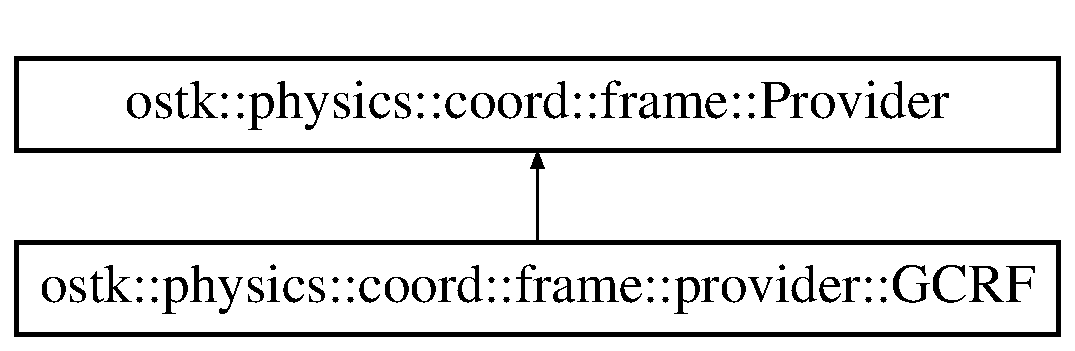
\includegraphics[height=2.000000cm]{classostk_1_1physics_1_1coord_1_1frame_1_1provider_1_1_g_c_r_f}
\end{center}
\end{figure}
\subsection*{Public Member Functions}
\begin{DoxyCompactItemize}
\item 
\hyperlink{classostk_1_1physics_1_1coord_1_1frame_1_1provider_1_1_g_c_r_f_a35f5f4903c6d64acc9fbd7285fe8f6bf}{G\+C\+RF} ()
\item 
virtual \hyperlink{classostk_1_1physics_1_1coord_1_1frame_1_1provider_1_1_g_c_r_f_aa02bee89fa910e3d6a76a8b68035e163}{$\sim$\+G\+C\+RF} () override
\item 
virtual \hyperlink{classostk_1_1physics_1_1coord_1_1frame_1_1provider_1_1_g_c_r_f}{G\+C\+RF} $\ast$ \hyperlink{classostk_1_1physics_1_1coord_1_1frame_1_1provider_1_1_g_c_r_f_a71f14cba2d0d20a5bbeaa3b4fb08a79a}{clone} () const override
\item 
virtual bool \hyperlink{classostk_1_1physics_1_1coord_1_1frame_1_1provider_1_1_g_c_r_f_a02160b74124b3ece74912c62aae5caaa}{is\+Defined} () const override
\item 
virtual \hyperlink{classostk_1_1physics_1_1coord_1_1_transform}{Transform} \hyperlink{classostk_1_1physics_1_1coord_1_1frame_1_1provider_1_1_g_c_r_f_a379dffe2291d4536dbdd65501fd28539}{get\+Transform\+At} (const \hyperlink{classostk_1_1physics_1_1time_1_1_instant}{Instant} \&an\+Instant) const override
\end{DoxyCompactItemize}


\subsection{Detailed Description}
Geocentric Celestial Reference \hyperlink{classostk_1_1physics_1_1coord_1_1_frame}{Frame} (\hyperlink{classostk_1_1physics_1_1coord_1_1frame_1_1provider_1_1_g_c_r_f}{G\+C\+RF}) provider. 

https\+://en.wikipedia.\+org/wiki/\+Earth-\/centered\+\_\+inertial 

\subsection{Constructor \& Destructor Documentation}
\mbox{\Hypertarget{classostk_1_1physics_1_1coord_1_1frame_1_1provider_1_1_g_c_r_f_a35f5f4903c6d64acc9fbd7285fe8f6bf}\label{classostk_1_1physics_1_1coord_1_1frame_1_1provider_1_1_g_c_r_f_a35f5f4903c6d64acc9fbd7285fe8f6bf}} 
\index{ostk\+::physics\+::coord\+::frame\+::provider\+::\+G\+C\+RF@{ostk\+::physics\+::coord\+::frame\+::provider\+::\+G\+C\+RF}!G\+C\+RF@{G\+C\+RF}}
\index{G\+C\+RF@{G\+C\+RF}!ostk\+::physics\+::coord\+::frame\+::provider\+::\+G\+C\+RF@{ostk\+::physics\+::coord\+::frame\+::provider\+::\+G\+C\+RF}}
\subsubsection{\texorpdfstring{G\+C\+R\+F()}{GCRF()}}
{\footnotesize\ttfamily ostk\+::physics\+::coord\+::frame\+::provider\+::\+G\+C\+R\+F\+::\+G\+C\+RF (\begin{DoxyParamCaption}{ }\end{DoxyParamCaption})}

\mbox{\Hypertarget{classostk_1_1physics_1_1coord_1_1frame_1_1provider_1_1_g_c_r_f_aa02bee89fa910e3d6a76a8b68035e163}\label{classostk_1_1physics_1_1coord_1_1frame_1_1provider_1_1_g_c_r_f_aa02bee89fa910e3d6a76a8b68035e163}} 
\index{ostk\+::physics\+::coord\+::frame\+::provider\+::\+G\+C\+RF@{ostk\+::physics\+::coord\+::frame\+::provider\+::\+G\+C\+RF}!````~G\+C\+RF@{$\sim$\+G\+C\+RF}}
\index{````~G\+C\+RF@{$\sim$\+G\+C\+RF}!ostk\+::physics\+::coord\+::frame\+::provider\+::\+G\+C\+RF@{ostk\+::physics\+::coord\+::frame\+::provider\+::\+G\+C\+RF}}
\subsubsection{\texorpdfstring{$\sim$\+G\+C\+R\+F()}{~GCRF()}}
{\footnotesize\ttfamily ostk\+::physics\+::coord\+::frame\+::provider\+::\+G\+C\+R\+F\+::$\sim$\+G\+C\+RF (\begin{DoxyParamCaption}{ }\end{DoxyParamCaption})\hspace{0.3cm}{\ttfamily [override]}, {\ttfamily [virtual]}}



\subsection{Member Function Documentation}
\mbox{\Hypertarget{classostk_1_1physics_1_1coord_1_1frame_1_1provider_1_1_g_c_r_f_a71f14cba2d0d20a5bbeaa3b4fb08a79a}\label{classostk_1_1physics_1_1coord_1_1frame_1_1provider_1_1_g_c_r_f_a71f14cba2d0d20a5bbeaa3b4fb08a79a}} 
\index{ostk\+::physics\+::coord\+::frame\+::provider\+::\+G\+C\+RF@{ostk\+::physics\+::coord\+::frame\+::provider\+::\+G\+C\+RF}!clone@{clone}}
\index{clone@{clone}!ostk\+::physics\+::coord\+::frame\+::provider\+::\+G\+C\+RF@{ostk\+::physics\+::coord\+::frame\+::provider\+::\+G\+C\+RF}}
\subsubsection{\texorpdfstring{clone()}{clone()}}
{\footnotesize\ttfamily \hyperlink{classostk_1_1physics_1_1coord_1_1frame_1_1provider_1_1_g_c_r_f}{G\+C\+RF} $\ast$ ostk\+::physics\+::coord\+::frame\+::provider\+::\+G\+C\+R\+F\+::clone (\begin{DoxyParamCaption}{ }\end{DoxyParamCaption}) const\hspace{0.3cm}{\ttfamily [override]}, {\ttfamily [virtual]}}



Implements \hyperlink{classostk_1_1physics_1_1coord_1_1frame_1_1_provider_ae41bc3862d088e9c8d90a79253294ce9}{ostk\+::physics\+::coord\+::frame\+::\+Provider}.

\mbox{\Hypertarget{classostk_1_1physics_1_1coord_1_1frame_1_1provider_1_1_g_c_r_f_a379dffe2291d4536dbdd65501fd28539}\label{classostk_1_1physics_1_1coord_1_1frame_1_1provider_1_1_g_c_r_f_a379dffe2291d4536dbdd65501fd28539}} 
\index{ostk\+::physics\+::coord\+::frame\+::provider\+::\+G\+C\+RF@{ostk\+::physics\+::coord\+::frame\+::provider\+::\+G\+C\+RF}!get\+Transform\+At@{get\+Transform\+At}}
\index{get\+Transform\+At@{get\+Transform\+At}!ostk\+::physics\+::coord\+::frame\+::provider\+::\+G\+C\+RF@{ostk\+::physics\+::coord\+::frame\+::provider\+::\+G\+C\+RF}}
\subsubsection{\texorpdfstring{get\+Transform\+At()}{getTransformAt()}}
{\footnotesize\ttfamily \hyperlink{classostk_1_1physics_1_1coord_1_1_transform}{Transform} ostk\+::physics\+::coord\+::frame\+::provider\+::\+G\+C\+R\+F\+::get\+Transform\+At (\begin{DoxyParamCaption}\item[{const \hyperlink{classostk_1_1physics_1_1time_1_1_instant}{Instant} \&}]{an\+Instant }\end{DoxyParamCaption}) const\hspace{0.3cm}{\ttfamily [override]}, {\ttfamily [virtual]}}



Implements \hyperlink{classostk_1_1physics_1_1coord_1_1frame_1_1_provider_a38b86a589f46f8b8a9c97ab2776f37d1}{ostk\+::physics\+::coord\+::frame\+::\+Provider}.

\mbox{\Hypertarget{classostk_1_1physics_1_1coord_1_1frame_1_1provider_1_1_g_c_r_f_a02160b74124b3ece74912c62aae5caaa}\label{classostk_1_1physics_1_1coord_1_1frame_1_1provider_1_1_g_c_r_f_a02160b74124b3ece74912c62aae5caaa}} 
\index{ostk\+::physics\+::coord\+::frame\+::provider\+::\+G\+C\+RF@{ostk\+::physics\+::coord\+::frame\+::provider\+::\+G\+C\+RF}!is\+Defined@{is\+Defined}}
\index{is\+Defined@{is\+Defined}!ostk\+::physics\+::coord\+::frame\+::provider\+::\+G\+C\+RF@{ostk\+::physics\+::coord\+::frame\+::provider\+::\+G\+C\+RF}}
\subsubsection{\texorpdfstring{is\+Defined()}{isDefined()}}
{\footnotesize\ttfamily bool ostk\+::physics\+::coord\+::frame\+::provider\+::\+G\+C\+R\+F\+::is\+Defined (\begin{DoxyParamCaption}{ }\end{DoxyParamCaption}) const\hspace{0.3cm}{\ttfamily [override]}, {\ttfamily [virtual]}}



Implements \hyperlink{classostk_1_1physics_1_1coord_1_1frame_1_1_provider_a27acab0012649796b97956fed1a91493}{ostk\+::physics\+::coord\+::frame\+::\+Provider}.



The documentation for this class was generated from the following files\+:\begin{DoxyCompactItemize}
\item 
include/\+Open\+Space\+Toolkit/\+Physics/\+Coordinate/\+Frame/\+Providers/\hyperlink{_g_c_r_f_8hpp}{G\+C\+R\+F.\+hpp}\item 
src/\+Open\+Space\+Toolkit/\+Physics/\+Coordinate/\+Frame/\+Providers/\hyperlink{_g_c_r_f_8cpp}{G\+C\+R\+F.\+cpp}\end{DoxyCompactItemize}

\hypertarget{classostk_1_1physics_1_1env_1_1object_1_1_geometry}{}\section{ostk\+:\+:physics\+:\+:env\+:\+:object\+:\+:Geometry Class Reference}
\label{classostk_1_1physics_1_1env_1_1object_1_1_geometry}\index{ostk\+::physics\+::env\+::object\+::\+Geometry@{ostk\+::physics\+::env\+::object\+::\+Geometry}}


{\ttfamily \#include $<$Geometry.\+hpp$>$}

\subsection*{Public Types}
\begin{DoxyCompactItemize}
\item 
typedef math\+::geom\+::d3\+::\+Object \hyperlink{classostk_1_1physics_1_1env_1_1object_1_1_geometry_abeade8931056612deaa868abdaac8c9c}{Object}
\end{DoxyCompactItemize}
\subsection*{Public Member Functions}
\begin{DoxyCompactItemize}
\item 
\hyperlink{classostk_1_1physics_1_1env_1_1object_1_1_geometry_a99cd68601f35dd7c24bb7e441728b65a}{Geometry} (const \hyperlink{classostk_1_1physics_1_1env_1_1object_1_1_geometry_abeade8931056612deaa868abdaac8c9c}{Geometry\+::\+Object} \&an\+Object, const Shared$<$ const \hyperlink{classostk_1_1physics_1_1coord_1_1_frame}{Frame} $>$ \&a\+Frame\+S\+Ptr)
\begin{DoxyCompactList}\small\item\em Constructor. \end{DoxyCompactList}\item 
\hyperlink{classostk_1_1physics_1_1env_1_1object_1_1_geometry_a0d841619ef4bc44ec3a98d412af9b1a7}{Geometry} (const Composite \&a\+Composite, const Shared$<$ const \hyperlink{classostk_1_1physics_1_1coord_1_1_frame}{Frame} $>$ \&a\+Frame\+S\+Ptr)
\begin{DoxyCompactList}\small\item\em Constructor. \end{DoxyCompactList}\item 
\hyperlink{classostk_1_1physics_1_1env_1_1object_1_1_geometry_a9b163b274588de65ad05290e421e0345}{Geometry} (const \hyperlink{classostk_1_1physics_1_1env_1_1object_1_1_geometry}{Geometry} \&a\+Geometry)
\begin{DoxyCompactList}\small\item\em Copy constructor. \end{DoxyCompactList}\item 
\hyperlink{classostk_1_1physics_1_1env_1_1object_1_1_geometry}{Geometry} \& \hyperlink{classostk_1_1physics_1_1env_1_1object_1_1_geometry_a777d72a587112d74bad356180f75b6d0}{operator=} (const \hyperlink{classostk_1_1physics_1_1env_1_1object_1_1_geometry}{Geometry} \&a\+Geometry)
\begin{DoxyCompactList}\small\item\em Copy assignment operator. \end{DoxyCompactList}\item 
bool \hyperlink{classostk_1_1physics_1_1env_1_1object_1_1_geometry_aa3d15f7a766995279b88ad7fdc2befe1}{operator==} (const \hyperlink{classostk_1_1physics_1_1env_1_1object_1_1_geometry}{Geometry} \&a\+Geometry) const
\begin{DoxyCompactList}\small\item\em Equal to operator. \end{DoxyCompactList}\item 
bool \hyperlink{classostk_1_1physics_1_1env_1_1object_1_1_geometry_ae47daffb1f1e7341706a771dce7bd2f2}{operator!=} (const \hyperlink{classostk_1_1physics_1_1env_1_1object_1_1_geometry}{Geometry} \&a\+Geometry) const
\begin{DoxyCompactList}\small\item\em Not equal to operator. \end{DoxyCompactList}\item 
bool \hyperlink{classostk_1_1physics_1_1env_1_1object_1_1_geometry_a46e3f9e3a85efd77a4df11fdfb544f4d}{is\+Defined} () const
\begin{DoxyCompactList}\small\item\em Check if geometry is defined. \end{DoxyCompactList}\item 
bool \hyperlink{classostk_1_1physics_1_1env_1_1object_1_1_geometry_adab144d62681369d1d456264dcab043c}{intersects} (const \hyperlink{classostk_1_1physics_1_1env_1_1object_1_1_geometry}{Geometry} \&a\+Geometry) const
\begin{DoxyCompactList}\small\item\em Check if geometry intersects another geometry. \end{DoxyCompactList}\item 
bool \hyperlink{classostk_1_1physics_1_1env_1_1object_1_1_geometry_ab08322d5d7639f1e22c0d6c2999c7e28}{contains} (const \hyperlink{classostk_1_1physics_1_1env_1_1object_1_1_geometry}{Geometry} \&a\+Geometry) const
\begin{DoxyCompactList}\small\item\em Check if geometry contains another geometry. \end{DoxyCompactList}\item 
const Composite \& \hyperlink{classostk_1_1physics_1_1env_1_1object_1_1_geometry_a993e5e8bd11e214ad6e3aee10c05cca4}{access\+Composite} () const
\begin{DoxyCompactList}\small\item\em Access composite. \end{DoxyCompactList}\item 
Shared$<$ const \hyperlink{classostk_1_1physics_1_1coord_1_1_frame}{Frame} $>$ \hyperlink{classostk_1_1physics_1_1env_1_1object_1_1_geometry_a5605bf833c7647eba5c32a88498876cb}{access\+Frame} () const
\begin{DoxyCompactList}\small\item\em Access frame. \end{DoxyCompactList}\item 
\hyperlink{classostk_1_1physics_1_1env_1_1object_1_1_geometry}{Geometry} \hyperlink{classostk_1_1physics_1_1env_1_1object_1_1_geometry_ac9d7aa217eb0ec8d0dff7270ca2d0447}{in} (const Shared$<$ const \hyperlink{classostk_1_1physics_1_1coord_1_1_frame}{Frame} $>$ \&a\+Frame\+S\+Ptr, const \hyperlink{classostk_1_1physics_1_1time_1_1_instant}{Instant} \&an\+Instant) const
\begin{DoxyCompactList}\small\item\em Get geometry expressed in a given frame. \end{DoxyCompactList}\item 
\hyperlink{classostk_1_1physics_1_1env_1_1object_1_1_geometry}{Geometry} \hyperlink{classostk_1_1physics_1_1env_1_1object_1_1_geometry_aee148ec3c78756b373d2e3b31ee2a34a}{intersection\+With} (const \hyperlink{classostk_1_1physics_1_1env_1_1object_1_1_geometry}{Geometry} \&a\+Geometry) const
\begin{DoxyCompactList}\small\item\em Compute intersection of geometry with another geometry. \end{DoxyCompactList}\end{DoxyCompactItemize}
\subsection*{Static Public Member Functions}
\begin{DoxyCompactItemize}
\item 
static \hyperlink{classostk_1_1physics_1_1env_1_1object_1_1_geometry}{Geometry} \hyperlink{classostk_1_1physics_1_1env_1_1object_1_1_geometry_a5954c3485fd2a21b1d1419e08a6dcc4e}{Undefined} ()
\begin{DoxyCompactList}\small\item\em Constructs an undefined geometry. \end{DoxyCompactList}\end{DoxyCompactItemize}
\subsection*{Friends}
\begin{DoxyCompactItemize}
\item 
std\+::ostream \& \hyperlink{classostk_1_1physics_1_1env_1_1object_1_1_geometry_aebfe5b9b5d8cd3dd8a2cfd140a1df583}{operator$<$$<$} (std\+::ostream \&an\+Output\+Stream, const \hyperlink{classostk_1_1physics_1_1env_1_1object_1_1_geometry}{Geometry} \&a\+Geometry)
\begin{DoxyCompactList}\small\item\em Output stream operator. \end{DoxyCompactList}\end{DoxyCompactItemize}


\subsection{Member Typedef Documentation}
\mbox{\Hypertarget{classostk_1_1physics_1_1env_1_1object_1_1_geometry_abeade8931056612deaa868abdaac8c9c}\label{classostk_1_1physics_1_1env_1_1object_1_1_geometry_abeade8931056612deaa868abdaac8c9c}} 
\index{ostk\+::physics\+::env\+::object\+::\+Geometry@{ostk\+::physics\+::env\+::object\+::\+Geometry}!Object@{Object}}
\index{Object@{Object}!ostk\+::physics\+::env\+::object\+::\+Geometry@{ostk\+::physics\+::env\+::object\+::\+Geometry}}
\subsubsection{\texorpdfstring{Object}{Object}}
{\footnotesize\ttfamily typedef math\+::geom\+::d3\+::\+Object \hyperlink{classostk_1_1physics_1_1env_1_1object_1_1_geometry_abeade8931056612deaa868abdaac8c9c}{ostk\+::physics\+::env\+::object\+::\+Geometry\+::\+Object}}



\subsection{Constructor \& Destructor Documentation}
\mbox{\Hypertarget{classostk_1_1physics_1_1env_1_1object_1_1_geometry_a99cd68601f35dd7c24bb7e441728b65a}\label{classostk_1_1physics_1_1env_1_1object_1_1_geometry_a99cd68601f35dd7c24bb7e441728b65a}} 
\index{ostk\+::physics\+::env\+::object\+::\+Geometry@{ostk\+::physics\+::env\+::object\+::\+Geometry}!Geometry@{Geometry}}
\index{Geometry@{Geometry}!ostk\+::physics\+::env\+::object\+::\+Geometry@{ostk\+::physics\+::env\+::object\+::\+Geometry}}
\subsubsection{\texorpdfstring{Geometry()}{Geometry()}\hspace{0.1cm}{\footnotesize\ttfamily [1/3]}}
{\footnotesize\ttfamily ostk\+::physics\+::env\+::object\+::\+Geometry\+::\+Geometry (\begin{DoxyParamCaption}\item[{const \hyperlink{classostk_1_1physics_1_1env_1_1object_1_1_geometry_abeade8931056612deaa868abdaac8c9c}{Geometry\+::\+Object} \&}]{an\+Object,  }\item[{const Shared$<$ const \hyperlink{classostk_1_1physics_1_1coord_1_1_frame}{Frame} $>$ \&}]{a\+Frame\+S\+Ptr }\end{DoxyParamCaption})}



Constructor. 


\begin{DoxyParams}[1]{Parameters}
\mbox{\tt in}  & {\em an\+Object} & An object \\
\hline
\mbox{\tt in}  & {\em a\+Frame\+S\+Ptr} & A shared pointer to frame \\
\hline
\end{DoxyParams}
\mbox{\Hypertarget{classostk_1_1physics_1_1env_1_1object_1_1_geometry_a0d841619ef4bc44ec3a98d412af9b1a7}\label{classostk_1_1physics_1_1env_1_1object_1_1_geometry_a0d841619ef4bc44ec3a98d412af9b1a7}} 
\index{ostk\+::physics\+::env\+::object\+::\+Geometry@{ostk\+::physics\+::env\+::object\+::\+Geometry}!Geometry@{Geometry}}
\index{Geometry@{Geometry}!ostk\+::physics\+::env\+::object\+::\+Geometry@{ostk\+::physics\+::env\+::object\+::\+Geometry}}
\subsubsection{\texorpdfstring{Geometry()}{Geometry()}\hspace{0.1cm}{\footnotesize\ttfamily [2/3]}}
{\footnotesize\ttfamily ostk\+::physics\+::env\+::object\+::\+Geometry\+::\+Geometry (\begin{DoxyParamCaption}\item[{const Composite \&}]{a\+Composite,  }\item[{const Shared$<$ const \hyperlink{classostk_1_1physics_1_1coord_1_1_frame}{Frame} $>$ \&}]{a\+Frame\+S\+Ptr }\end{DoxyParamCaption})}



Constructor. 


\begin{DoxyParams}[1]{Parameters}
\mbox{\tt in}  & {\em a\+Composite} & A composite \\
\hline
\mbox{\tt in}  & {\em a\+Frame\+S\+Ptr} & A shared pointer to frame \\
\hline
\end{DoxyParams}
\mbox{\Hypertarget{classostk_1_1physics_1_1env_1_1object_1_1_geometry_a9b163b274588de65ad05290e421e0345}\label{classostk_1_1physics_1_1env_1_1object_1_1_geometry_a9b163b274588de65ad05290e421e0345}} 
\index{ostk\+::physics\+::env\+::object\+::\+Geometry@{ostk\+::physics\+::env\+::object\+::\+Geometry}!Geometry@{Geometry}}
\index{Geometry@{Geometry}!ostk\+::physics\+::env\+::object\+::\+Geometry@{ostk\+::physics\+::env\+::object\+::\+Geometry}}
\subsubsection{\texorpdfstring{Geometry()}{Geometry()}\hspace{0.1cm}{\footnotesize\ttfamily [3/3]}}
{\footnotesize\ttfamily ostk\+::physics\+::env\+::object\+::\+Geometry\+::\+Geometry (\begin{DoxyParamCaption}\item[{const \hyperlink{classostk_1_1physics_1_1env_1_1object_1_1_geometry}{Geometry} \&}]{a\+Geometry }\end{DoxyParamCaption})}



Copy constructor. 


\begin{DoxyParams}[1]{Parameters}
\mbox{\tt in}  & {\em a\+Geometry} & A geometry \\
\hline
\end{DoxyParams}


\subsection{Member Function Documentation}
\mbox{\Hypertarget{classostk_1_1physics_1_1env_1_1object_1_1_geometry_a993e5e8bd11e214ad6e3aee10c05cca4}\label{classostk_1_1physics_1_1env_1_1object_1_1_geometry_a993e5e8bd11e214ad6e3aee10c05cca4}} 
\index{ostk\+::physics\+::env\+::object\+::\+Geometry@{ostk\+::physics\+::env\+::object\+::\+Geometry}!access\+Composite@{access\+Composite}}
\index{access\+Composite@{access\+Composite}!ostk\+::physics\+::env\+::object\+::\+Geometry@{ostk\+::physics\+::env\+::object\+::\+Geometry}}
\subsubsection{\texorpdfstring{access\+Composite()}{accessComposite()}}
{\footnotesize\ttfamily const Composite \& ostk\+::physics\+::env\+::object\+::\+Geometry\+::access\+Composite (\begin{DoxyParamCaption}{ }\end{DoxyParamCaption}) const}



Access composite. 

\begin{DoxyReturn}{Returns}
Reference to composite 
\end{DoxyReturn}
\mbox{\Hypertarget{classostk_1_1physics_1_1env_1_1object_1_1_geometry_a5605bf833c7647eba5c32a88498876cb}\label{classostk_1_1physics_1_1env_1_1object_1_1_geometry_a5605bf833c7647eba5c32a88498876cb}} 
\index{ostk\+::physics\+::env\+::object\+::\+Geometry@{ostk\+::physics\+::env\+::object\+::\+Geometry}!access\+Frame@{access\+Frame}}
\index{access\+Frame@{access\+Frame}!ostk\+::physics\+::env\+::object\+::\+Geometry@{ostk\+::physics\+::env\+::object\+::\+Geometry}}
\subsubsection{\texorpdfstring{access\+Frame()}{accessFrame()}}
{\footnotesize\ttfamily Shared$<$ const \hyperlink{classostk_1_1physics_1_1coord_1_1_frame}{Frame} $>$ ostk\+::physics\+::env\+::object\+::\+Geometry\+::access\+Frame (\begin{DoxyParamCaption}{ }\end{DoxyParamCaption}) const}



Access frame. 

\begin{DoxyReturn}{Returns}
Shared pointer to frame 
\end{DoxyReturn}
\mbox{\Hypertarget{classostk_1_1physics_1_1env_1_1object_1_1_geometry_ab08322d5d7639f1e22c0d6c2999c7e28}\label{classostk_1_1physics_1_1env_1_1object_1_1_geometry_ab08322d5d7639f1e22c0d6c2999c7e28}} 
\index{ostk\+::physics\+::env\+::object\+::\+Geometry@{ostk\+::physics\+::env\+::object\+::\+Geometry}!contains@{contains}}
\index{contains@{contains}!ostk\+::physics\+::env\+::object\+::\+Geometry@{ostk\+::physics\+::env\+::object\+::\+Geometry}}
\subsubsection{\texorpdfstring{contains()}{contains()}}
{\footnotesize\ttfamily bool ostk\+::physics\+::env\+::object\+::\+Geometry\+::contains (\begin{DoxyParamCaption}\item[{const \hyperlink{classostk_1_1physics_1_1env_1_1object_1_1_geometry}{Geometry} \&}]{a\+Geometry }\end{DoxyParamCaption}) const}



Check if geometry contains another geometry. 


\begin{DoxyParams}[1]{Parameters}
\mbox{\tt in}  & {\em a\+Geometry} & A geometry \\
\hline
\end{DoxyParams}
\begin{DoxyReturn}{Returns}
True if geometry contains another geometry 
\end{DoxyReturn}
\mbox{\Hypertarget{classostk_1_1physics_1_1env_1_1object_1_1_geometry_ac9d7aa217eb0ec8d0dff7270ca2d0447}\label{classostk_1_1physics_1_1env_1_1object_1_1_geometry_ac9d7aa217eb0ec8d0dff7270ca2d0447}} 
\index{ostk\+::physics\+::env\+::object\+::\+Geometry@{ostk\+::physics\+::env\+::object\+::\+Geometry}!in@{in}}
\index{in@{in}!ostk\+::physics\+::env\+::object\+::\+Geometry@{ostk\+::physics\+::env\+::object\+::\+Geometry}}
\subsubsection{\texorpdfstring{in()}{in()}}
{\footnotesize\ttfamily \hyperlink{classostk_1_1physics_1_1env_1_1object_1_1_geometry}{Geometry} ostk\+::physics\+::env\+::object\+::\+Geometry\+::in (\begin{DoxyParamCaption}\item[{const Shared$<$ const \hyperlink{classostk_1_1physics_1_1coord_1_1_frame}{Frame} $>$ \&}]{a\+Frame\+S\+Ptr,  }\item[{const \hyperlink{classostk_1_1physics_1_1time_1_1_instant}{Instant} \&}]{an\+Instant }\end{DoxyParamCaption}) const}



Get geometry expressed in a given frame. 


\begin{DoxyParams}[1]{Parameters}
\mbox{\tt in}  & {\em a\+Frame\+S\+Ptr} & A shared pointer to frame \\
\hline
\mbox{\tt in}  & {\em an\+Instant} & An instant \\
\hline
\end{DoxyParams}
\begin{DoxyReturn}{Returns}
\hyperlink{classostk_1_1physics_1_1env_1_1object_1_1_geometry}{Geometry} expressed in a given frame 
\end{DoxyReturn}
\mbox{\Hypertarget{classostk_1_1physics_1_1env_1_1object_1_1_geometry_aee148ec3c78756b373d2e3b31ee2a34a}\label{classostk_1_1physics_1_1env_1_1object_1_1_geometry_aee148ec3c78756b373d2e3b31ee2a34a}} 
\index{ostk\+::physics\+::env\+::object\+::\+Geometry@{ostk\+::physics\+::env\+::object\+::\+Geometry}!intersection\+With@{intersection\+With}}
\index{intersection\+With@{intersection\+With}!ostk\+::physics\+::env\+::object\+::\+Geometry@{ostk\+::physics\+::env\+::object\+::\+Geometry}}
\subsubsection{\texorpdfstring{intersection\+With()}{intersectionWith()}}
{\footnotesize\ttfamily \hyperlink{classostk_1_1physics_1_1env_1_1object_1_1_geometry}{Geometry} ostk\+::physics\+::env\+::object\+::\+Geometry\+::intersection\+With (\begin{DoxyParamCaption}\item[{const \hyperlink{classostk_1_1physics_1_1env_1_1object_1_1_geometry}{Geometry} \&}]{a\+Geometry }\end{DoxyParamCaption}) const}



Compute intersection of geometry with another geometry. 


\begin{DoxyParams}[1]{Parameters}
\mbox{\tt in}  & {\em a\+Geometry} & A geometry \\
\hline
\end{DoxyParams}
\begin{DoxyReturn}{Returns}
Intersection of geometry with another geometry 
\end{DoxyReturn}
\mbox{\Hypertarget{classostk_1_1physics_1_1env_1_1object_1_1_geometry_adab144d62681369d1d456264dcab043c}\label{classostk_1_1physics_1_1env_1_1object_1_1_geometry_adab144d62681369d1d456264dcab043c}} 
\index{ostk\+::physics\+::env\+::object\+::\+Geometry@{ostk\+::physics\+::env\+::object\+::\+Geometry}!intersects@{intersects}}
\index{intersects@{intersects}!ostk\+::physics\+::env\+::object\+::\+Geometry@{ostk\+::physics\+::env\+::object\+::\+Geometry}}
\subsubsection{\texorpdfstring{intersects()}{intersects()}}
{\footnotesize\ttfamily bool ostk\+::physics\+::env\+::object\+::\+Geometry\+::intersects (\begin{DoxyParamCaption}\item[{const \hyperlink{classostk_1_1physics_1_1env_1_1object_1_1_geometry}{Geometry} \&}]{a\+Geometry }\end{DoxyParamCaption}) const}



Check if geometry intersects another geometry. 


\begin{DoxyParams}[1]{Parameters}
\mbox{\tt in}  & {\em a\+Geometry} & A geometry \\
\hline
\end{DoxyParams}
\begin{DoxyReturn}{Returns}
True if geometry intersects another geometry 
\end{DoxyReturn}
\mbox{\Hypertarget{classostk_1_1physics_1_1env_1_1object_1_1_geometry_a46e3f9e3a85efd77a4df11fdfb544f4d}\label{classostk_1_1physics_1_1env_1_1object_1_1_geometry_a46e3f9e3a85efd77a4df11fdfb544f4d}} 
\index{ostk\+::physics\+::env\+::object\+::\+Geometry@{ostk\+::physics\+::env\+::object\+::\+Geometry}!is\+Defined@{is\+Defined}}
\index{is\+Defined@{is\+Defined}!ostk\+::physics\+::env\+::object\+::\+Geometry@{ostk\+::physics\+::env\+::object\+::\+Geometry}}
\subsubsection{\texorpdfstring{is\+Defined()}{isDefined()}}
{\footnotesize\ttfamily bool ostk\+::physics\+::env\+::object\+::\+Geometry\+::is\+Defined (\begin{DoxyParamCaption}{ }\end{DoxyParamCaption}) const}



Check if geometry is defined. 

\begin{DoxyReturn}{Returns}
True if geometry is defined 
\end{DoxyReturn}
\mbox{\Hypertarget{classostk_1_1physics_1_1env_1_1object_1_1_geometry_ae47daffb1f1e7341706a771dce7bd2f2}\label{classostk_1_1physics_1_1env_1_1object_1_1_geometry_ae47daffb1f1e7341706a771dce7bd2f2}} 
\index{ostk\+::physics\+::env\+::object\+::\+Geometry@{ostk\+::physics\+::env\+::object\+::\+Geometry}!operator"!=@{operator"!=}}
\index{operator"!=@{operator"!=}!ostk\+::physics\+::env\+::object\+::\+Geometry@{ostk\+::physics\+::env\+::object\+::\+Geometry}}
\subsubsection{\texorpdfstring{operator"!=()}{operator!=()}}
{\footnotesize\ttfamily bool ostk\+::physics\+::env\+::object\+::\+Geometry\+::operator!= (\begin{DoxyParamCaption}\item[{const \hyperlink{classostk_1_1physics_1_1env_1_1object_1_1_geometry}{Geometry} \&}]{a\+Geometry }\end{DoxyParamCaption}) const}



Not equal to operator. 


\begin{DoxyParams}[1]{Parameters}
\mbox{\tt in}  & {\em a\+Geometry} & A geometry \\
\hline
\end{DoxyParams}
\begin{DoxyReturn}{Returns}
True if geometries are not equal 
\end{DoxyReturn}
\mbox{\Hypertarget{classostk_1_1physics_1_1env_1_1object_1_1_geometry_a777d72a587112d74bad356180f75b6d0}\label{classostk_1_1physics_1_1env_1_1object_1_1_geometry_a777d72a587112d74bad356180f75b6d0}} 
\index{ostk\+::physics\+::env\+::object\+::\+Geometry@{ostk\+::physics\+::env\+::object\+::\+Geometry}!operator=@{operator=}}
\index{operator=@{operator=}!ostk\+::physics\+::env\+::object\+::\+Geometry@{ostk\+::physics\+::env\+::object\+::\+Geometry}}
\subsubsection{\texorpdfstring{operator=()}{operator=()}}
{\footnotesize\ttfamily \hyperlink{classostk_1_1physics_1_1env_1_1object_1_1_geometry}{Geometry} \& ostk\+::physics\+::env\+::object\+::\+Geometry\+::operator= (\begin{DoxyParamCaption}\item[{const \hyperlink{classostk_1_1physics_1_1env_1_1object_1_1_geometry}{Geometry} \&}]{a\+Geometry }\end{DoxyParamCaption})}



Copy assignment operator. 


\begin{DoxyParams}[1]{Parameters}
\mbox{\tt in}  & {\em a\+Geometry} & A geometry \\
\hline
\end{DoxyParams}
\begin{DoxyReturn}{Returns}
Reference to geometry 
\end{DoxyReturn}
\mbox{\Hypertarget{classostk_1_1physics_1_1env_1_1object_1_1_geometry_aa3d15f7a766995279b88ad7fdc2befe1}\label{classostk_1_1physics_1_1env_1_1object_1_1_geometry_aa3d15f7a766995279b88ad7fdc2befe1}} 
\index{ostk\+::physics\+::env\+::object\+::\+Geometry@{ostk\+::physics\+::env\+::object\+::\+Geometry}!operator==@{operator==}}
\index{operator==@{operator==}!ostk\+::physics\+::env\+::object\+::\+Geometry@{ostk\+::physics\+::env\+::object\+::\+Geometry}}
\subsubsection{\texorpdfstring{operator==()}{operator==()}}
{\footnotesize\ttfamily bool ostk\+::physics\+::env\+::object\+::\+Geometry\+::operator== (\begin{DoxyParamCaption}\item[{const \hyperlink{classostk_1_1physics_1_1env_1_1object_1_1_geometry}{Geometry} \&}]{a\+Geometry }\end{DoxyParamCaption}) const}



Equal to operator. 


\begin{DoxyParams}[1]{Parameters}
\mbox{\tt in}  & {\em a\+Geometry} & A geometry \\
\hline
\end{DoxyParams}
\begin{DoxyReturn}{Returns}
True if geometries are equal 
\end{DoxyReturn}
\mbox{\Hypertarget{classostk_1_1physics_1_1env_1_1object_1_1_geometry_a5954c3485fd2a21b1d1419e08a6dcc4e}\label{classostk_1_1physics_1_1env_1_1object_1_1_geometry_a5954c3485fd2a21b1d1419e08a6dcc4e}} 
\index{ostk\+::physics\+::env\+::object\+::\+Geometry@{ostk\+::physics\+::env\+::object\+::\+Geometry}!Undefined@{Undefined}}
\index{Undefined@{Undefined}!ostk\+::physics\+::env\+::object\+::\+Geometry@{ostk\+::physics\+::env\+::object\+::\+Geometry}}
\subsubsection{\texorpdfstring{Undefined()}{Undefined()}}
{\footnotesize\ttfamily \hyperlink{classostk_1_1physics_1_1env_1_1object_1_1_geometry}{Geometry} ostk\+::physics\+::env\+::object\+::\+Geometry\+::\+Undefined (\begin{DoxyParamCaption}{ }\end{DoxyParamCaption})\hspace{0.3cm}{\ttfamily [static]}}



Constructs an undefined geometry. 


\begin{DoxyCode}
\hyperlink{classostk_1_1physics_1_1env_1_1object_1_1_geometry_a99cd68601f35dd7c24bb7e441728b65a}{Geometry} geometry = \hyperlink{classostk_1_1physics_1_1env_1_1object_1_1_geometry_a5954c3485fd2a21b1d1419e08a6dcc4e}{Geometry::Undefined}() ; \textcolor{comment}{// Undefined}
\end{DoxyCode}


\begin{DoxyReturn}{Returns}
Undefined geometry 
\end{DoxyReturn}


\subsection{Friends And Related Function Documentation}
\mbox{\Hypertarget{classostk_1_1physics_1_1env_1_1object_1_1_geometry_aebfe5b9b5d8cd3dd8a2cfd140a1df583}\label{classostk_1_1physics_1_1env_1_1object_1_1_geometry_aebfe5b9b5d8cd3dd8a2cfd140a1df583}} 
\index{ostk\+::physics\+::env\+::object\+::\+Geometry@{ostk\+::physics\+::env\+::object\+::\+Geometry}!operator$<$$<$@{operator$<$$<$}}
\index{operator$<$$<$@{operator$<$$<$}!ostk\+::physics\+::env\+::object\+::\+Geometry@{ostk\+::physics\+::env\+::object\+::\+Geometry}}
\subsubsection{\texorpdfstring{operator$<$$<$}{operator<<}}
{\footnotesize\ttfamily std\+::ostream\& operator$<$$<$ (\begin{DoxyParamCaption}\item[{std\+::ostream \&}]{an\+Output\+Stream,  }\item[{const \hyperlink{classostk_1_1physics_1_1env_1_1object_1_1_geometry}{Geometry} \&}]{a\+Geometry }\end{DoxyParamCaption})\hspace{0.3cm}{\ttfamily [friend]}}



Output stream operator. 


\begin{DoxyParams}[1]{Parameters}
\mbox{\tt in}  & {\em an\+Output\+Stream} & An output stream \\
\hline
\mbox{\tt in}  & {\em a\+Geometry} & A geometry \\
\hline
\end{DoxyParams}
\begin{DoxyReturn}{Returns}
A reference to output stream 
\end{DoxyReturn}


The documentation for this class was generated from the following files\+:\begin{DoxyCompactItemize}
\item 
include/\+Open\+Space\+Toolkit/\+Physics/\+Environment/\+Object/\hyperlink{_geometry_8hpp}{Geometry.\+hpp}\item 
src/\+Open\+Space\+Toolkit/\+Physics/\+Environment/\+Object/\hyperlink{_geometry_8cpp}{Geometry.\+cpp}\end{DoxyCompactItemize}

\hypertarget{classostk_1_1physics_1_1coord_1_1frame_1_1provider_1_1_i_c_r_f}{}\section{ostk\+:\+:physics\+:\+:coord\+:\+:frame\+:\+:provider\+:\+:I\+C\+RF Class Reference}
\label{classostk_1_1physics_1_1coord_1_1frame_1_1provider_1_1_i_c_r_f}\index{ostk\+::physics\+::coord\+::frame\+::provider\+::\+I\+C\+RF@{ostk\+::physics\+::coord\+::frame\+::provider\+::\+I\+C\+RF}}


International Celestial Reference \hyperlink{classostk_1_1physics_1_1coord_1_1_frame}{Frame} (\hyperlink{classostk_1_1physics_1_1coord_1_1frame_1_1provider_1_1_i_c_r_f}{I\+C\+RF}) provider.  




{\ttfamily \#include $<$I\+C\+R\+F.\+hpp$>$}

Inheritance diagram for ostk\+:\+:physics\+:\+:coord\+:\+:frame\+:\+:provider\+:\+:I\+C\+RF\+:\begin{figure}[H]
\begin{center}
\leavevmode
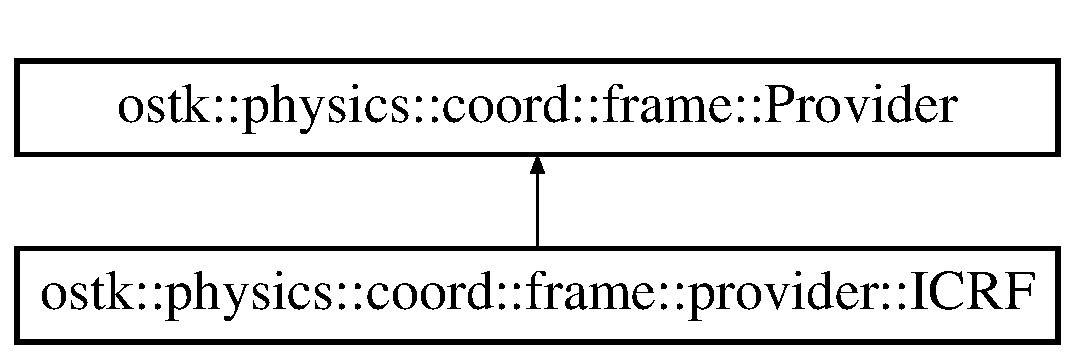
\includegraphics[height=2.000000cm]{classostk_1_1physics_1_1coord_1_1frame_1_1provider_1_1_i_c_r_f}
\end{center}
\end{figure}
\subsection*{Public Member Functions}
\begin{DoxyCompactItemize}
\item 
\hyperlink{classostk_1_1physics_1_1coord_1_1frame_1_1provider_1_1_i_c_r_f_a4ee5db5699238f12a9846f4440c6b926}{I\+C\+RF} ()
\item 
virtual \hyperlink{classostk_1_1physics_1_1coord_1_1frame_1_1provider_1_1_i_c_r_f_a9466870694d2b16fc116b1df36675dbc}{$\sim$\+I\+C\+RF} () override
\item 
virtual \hyperlink{classostk_1_1physics_1_1coord_1_1frame_1_1provider_1_1_i_c_r_f}{I\+C\+RF} $\ast$ \hyperlink{classostk_1_1physics_1_1coord_1_1frame_1_1provider_1_1_i_c_r_f_a40f7812d39719db68178ab6850a5cdde}{clone} () const override
\item 
virtual bool \hyperlink{classostk_1_1physics_1_1coord_1_1frame_1_1provider_1_1_i_c_r_f_a0d8e56478597e46dbc2c1867e6774398}{is\+Defined} () const override
\item 
virtual \hyperlink{classostk_1_1physics_1_1coord_1_1_transform}{Transform} \hyperlink{classostk_1_1physics_1_1coord_1_1frame_1_1provider_1_1_i_c_r_f_ab8d3ba4c098340eb43583e80cb5dd826}{get\+Transform\+At} (const \hyperlink{classostk_1_1physics_1_1time_1_1_instant}{Instant} \&an\+Instant) const override
\end{DoxyCompactItemize}


\subsection{Detailed Description}
International Celestial Reference \hyperlink{classostk_1_1physics_1_1coord_1_1_frame}{Frame} (\hyperlink{classostk_1_1physics_1_1coord_1_1frame_1_1provider_1_1_i_c_r_f}{I\+C\+RF}) provider. 

https\+://en.wikipedia.\+org/wiki/\+International\+\_\+\+Celestial\+\_\+\+Reference\+\_\+\+Frame 

\subsection{Constructor \& Destructor Documentation}
\mbox{\Hypertarget{classostk_1_1physics_1_1coord_1_1frame_1_1provider_1_1_i_c_r_f_a4ee5db5699238f12a9846f4440c6b926}\label{classostk_1_1physics_1_1coord_1_1frame_1_1provider_1_1_i_c_r_f_a4ee5db5699238f12a9846f4440c6b926}} 
\index{ostk\+::physics\+::coord\+::frame\+::provider\+::\+I\+C\+RF@{ostk\+::physics\+::coord\+::frame\+::provider\+::\+I\+C\+RF}!I\+C\+RF@{I\+C\+RF}}
\index{I\+C\+RF@{I\+C\+RF}!ostk\+::physics\+::coord\+::frame\+::provider\+::\+I\+C\+RF@{ostk\+::physics\+::coord\+::frame\+::provider\+::\+I\+C\+RF}}
\subsubsection{\texorpdfstring{I\+C\+R\+F()}{ICRF()}}
{\footnotesize\ttfamily ostk\+::physics\+::coord\+::frame\+::provider\+::\+I\+C\+R\+F\+::\+I\+C\+RF (\begin{DoxyParamCaption}{ }\end{DoxyParamCaption})}

\mbox{\Hypertarget{classostk_1_1physics_1_1coord_1_1frame_1_1provider_1_1_i_c_r_f_a9466870694d2b16fc116b1df36675dbc}\label{classostk_1_1physics_1_1coord_1_1frame_1_1provider_1_1_i_c_r_f_a9466870694d2b16fc116b1df36675dbc}} 
\index{ostk\+::physics\+::coord\+::frame\+::provider\+::\+I\+C\+RF@{ostk\+::physics\+::coord\+::frame\+::provider\+::\+I\+C\+RF}!````~I\+C\+RF@{$\sim$\+I\+C\+RF}}
\index{````~I\+C\+RF@{$\sim$\+I\+C\+RF}!ostk\+::physics\+::coord\+::frame\+::provider\+::\+I\+C\+RF@{ostk\+::physics\+::coord\+::frame\+::provider\+::\+I\+C\+RF}}
\subsubsection{\texorpdfstring{$\sim$\+I\+C\+R\+F()}{~ICRF()}}
{\footnotesize\ttfamily ostk\+::physics\+::coord\+::frame\+::provider\+::\+I\+C\+R\+F\+::$\sim$\+I\+C\+RF (\begin{DoxyParamCaption}{ }\end{DoxyParamCaption})\hspace{0.3cm}{\ttfamily [override]}, {\ttfamily [virtual]}}



\subsection{Member Function Documentation}
\mbox{\Hypertarget{classostk_1_1physics_1_1coord_1_1frame_1_1provider_1_1_i_c_r_f_a40f7812d39719db68178ab6850a5cdde}\label{classostk_1_1physics_1_1coord_1_1frame_1_1provider_1_1_i_c_r_f_a40f7812d39719db68178ab6850a5cdde}} 
\index{ostk\+::physics\+::coord\+::frame\+::provider\+::\+I\+C\+RF@{ostk\+::physics\+::coord\+::frame\+::provider\+::\+I\+C\+RF}!clone@{clone}}
\index{clone@{clone}!ostk\+::physics\+::coord\+::frame\+::provider\+::\+I\+C\+RF@{ostk\+::physics\+::coord\+::frame\+::provider\+::\+I\+C\+RF}}
\subsubsection{\texorpdfstring{clone()}{clone()}}
{\footnotesize\ttfamily \hyperlink{classostk_1_1physics_1_1coord_1_1frame_1_1provider_1_1_i_c_r_f}{I\+C\+RF} $\ast$ ostk\+::physics\+::coord\+::frame\+::provider\+::\+I\+C\+R\+F\+::clone (\begin{DoxyParamCaption}{ }\end{DoxyParamCaption}) const\hspace{0.3cm}{\ttfamily [override]}, {\ttfamily [virtual]}}



Implements \hyperlink{classostk_1_1physics_1_1coord_1_1frame_1_1_provider_ae41bc3862d088e9c8d90a79253294ce9}{ostk\+::physics\+::coord\+::frame\+::\+Provider}.

\mbox{\Hypertarget{classostk_1_1physics_1_1coord_1_1frame_1_1provider_1_1_i_c_r_f_ab8d3ba4c098340eb43583e80cb5dd826}\label{classostk_1_1physics_1_1coord_1_1frame_1_1provider_1_1_i_c_r_f_ab8d3ba4c098340eb43583e80cb5dd826}} 
\index{ostk\+::physics\+::coord\+::frame\+::provider\+::\+I\+C\+RF@{ostk\+::physics\+::coord\+::frame\+::provider\+::\+I\+C\+RF}!get\+Transform\+At@{get\+Transform\+At}}
\index{get\+Transform\+At@{get\+Transform\+At}!ostk\+::physics\+::coord\+::frame\+::provider\+::\+I\+C\+RF@{ostk\+::physics\+::coord\+::frame\+::provider\+::\+I\+C\+RF}}
\subsubsection{\texorpdfstring{get\+Transform\+At()}{getTransformAt()}}
{\footnotesize\ttfamily \hyperlink{classostk_1_1physics_1_1coord_1_1_transform}{Transform} ostk\+::physics\+::coord\+::frame\+::provider\+::\+I\+C\+R\+F\+::get\+Transform\+At (\begin{DoxyParamCaption}\item[{const \hyperlink{classostk_1_1physics_1_1time_1_1_instant}{Instant} \&}]{an\+Instant }\end{DoxyParamCaption}) const\hspace{0.3cm}{\ttfamily [override]}, {\ttfamily [virtual]}}



Implements \hyperlink{classostk_1_1physics_1_1coord_1_1frame_1_1_provider_a38b86a589f46f8b8a9c97ab2776f37d1}{ostk\+::physics\+::coord\+::frame\+::\+Provider}.

\mbox{\Hypertarget{classostk_1_1physics_1_1coord_1_1frame_1_1provider_1_1_i_c_r_f_a0d8e56478597e46dbc2c1867e6774398}\label{classostk_1_1physics_1_1coord_1_1frame_1_1provider_1_1_i_c_r_f_a0d8e56478597e46dbc2c1867e6774398}} 
\index{ostk\+::physics\+::coord\+::frame\+::provider\+::\+I\+C\+RF@{ostk\+::physics\+::coord\+::frame\+::provider\+::\+I\+C\+RF}!is\+Defined@{is\+Defined}}
\index{is\+Defined@{is\+Defined}!ostk\+::physics\+::coord\+::frame\+::provider\+::\+I\+C\+RF@{ostk\+::physics\+::coord\+::frame\+::provider\+::\+I\+C\+RF}}
\subsubsection{\texorpdfstring{is\+Defined()}{isDefined()}}
{\footnotesize\ttfamily bool ostk\+::physics\+::coord\+::frame\+::provider\+::\+I\+C\+R\+F\+::is\+Defined (\begin{DoxyParamCaption}{ }\end{DoxyParamCaption}) const\hspace{0.3cm}{\ttfamily [override]}, {\ttfamily [virtual]}}



Implements \hyperlink{classostk_1_1physics_1_1coord_1_1frame_1_1_provider_a27acab0012649796b97956fed1a91493}{ostk\+::physics\+::coord\+::frame\+::\+Provider}.



The documentation for this class was generated from the following files\+:\begin{DoxyCompactItemize}
\item 
include/\+Open\+Space\+Toolkit/\+Physics/\+Coordinate/\+Frame/\+Providers/\hyperlink{_i_c_r_f_8hpp}{I\+C\+R\+F.\+hpp}\item 
src/\+Open\+Space\+Toolkit/\+Physics/\+Coordinate/\+Frame/\+Providers/\hyperlink{_i_c_r_f_8cpp}{I\+C\+R\+F.\+cpp}\end{DoxyCompactItemize}

\hypertarget{classostk_1_1physics_1_1env_1_1ephem_1_1spice_1_1_index}{}\section{ostk\+:\+:physics\+:\+:env\+:\+:ephem\+:\+:spice\+:\+:Index Class Reference}
\label{classostk_1_1physics_1_1env_1_1ephem_1_1spice_1_1_index}\index{ostk\+::physics\+::env\+::ephem\+::spice\+::\+Index@{ostk\+::physics\+::env\+::ephem\+::spice\+::\+Index}}


\hyperlink{classostk_1_1physics_1_1env_1_1ephem_1_1_s_p_i_c_e}{S\+P\+I\+CE} Toolkit kernel index.  




{\ttfamily \#include $<$Index.\+hpp$>$}

\subsection*{Public Member Functions}
\begin{DoxyCompactItemize}
\item 
bool \hyperlink{classostk_1_1physics_1_1env_1_1ephem_1_1spice_1_1_index_a4c94c88d8e3fe896eaaa2baa1c0b3bb8}{is\+Empty} () const
\begin{DoxyCompactList}\small\item\em Returns true if index is empty. \end{DoxyCompactList}\item 
\hyperlink{classostk_1_1physics_1_1time_1_1_instant}{Instant} \hyperlink{classostk_1_1physics_1_1env_1_1ephem_1_1spice_1_1_index_ac9084f3d77dbe04d460ee335907fab83}{get\+Timestamp} () const
\begin{DoxyCompactList}\small\item\em Get index timestamp. \end{DoxyCompactList}\item 
U\+RL \hyperlink{classostk_1_1physics_1_1env_1_1ephem_1_1spice_1_1_index_a486ec6dad159dfdee2436be60ba5eb20}{get\+Remote\+Url\+Of\+Kernel} (const \hyperlink{classostk_1_1physics_1_1env_1_1ephem_1_1spice_1_1_kernel}{Kernel} \&a\+Kernel) const
\begin{DoxyCompactList}\small\item\em Get remote U\+RL of kernel. \end{DoxyCompactList}\item 
Array$<$ U\+RL $>$ \hyperlink{classostk_1_1physics_1_1env_1_1ephem_1_1spice_1_1_index_aa2bc4acdf1f1d209cb0fbe0f9a49a3f4}{find\+Remote\+Urls} (const std\+::regex \&a\+Kernel\+Name\+Regex) const
\begin{DoxyCompactList}\small\item\em Find remote U\+R\+Ls of kernels matching regular expression. \end{DoxyCompactList}\end{DoxyCompactItemize}
\subsection*{Static Public Member Functions}
\begin{DoxyCompactItemize}
\item 
static \hyperlink{classostk_1_1physics_1_1env_1_1ephem_1_1spice_1_1_index}{Index} \hyperlink{classostk_1_1physics_1_1env_1_1ephem_1_1spice_1_1_index_ac6afccc60da38e217e01f83b9f1c8d7a}{Empty} ()
\begin{DoxyCompactList}\small\item\em Constructs an empty index. \end{DoxyCompactList}\item 
static \hyperlink{classostk_1_1physics_1_1env_1_1ephem_1_1spice_1_1_index}{Index} \hyperlink{classostk_1_1physics_1_1env_1_1ephem_1_1spice_1_1_index_a73345e080ebf9a86f3447c5049892925}{Load} (const File \&a\+File)
\begin{DoxyCompactList}\small\item\em Load index from file. \end{DoxyCompactList}\end{DoxyCompactItemize}
\subsection*{Friends}
\begin{DoxyCompactItemize}
\item 
std\+::ostream \& \hyperlink{classostk_1_1physics_1_1env_1_1ephem_1_1spice_1_1_index_a1cdcc2b37f330da2f47a459f6225e98d}{operator$<$$<$} (std\+::ostream \&an\+Output\+Stream, const \hyperlink{classostk_1_1physics_1_1env_1_1ephem_1_1spice_1_1_index}{Index} \&an\+Index)
\begin{DoxyCompactList}\small\item\em Output stream operator. \end{DoxyCompactList}\end{DoxyCompactItemize}


\subsection{Detailed Description}
\hyperlink{classostk_1_1physics_1_1env_1_1ephem_1_1_s_p_i_c_e}{S\+P\+I\+CE} Toolkit kernel index. 

\subsection{Member Function Documentation}
\mbox{\Hypertarget{classostk_1_1physics_1_1env_1_1ephem_1_1spice_1_1_index_ac6afccc60da38e217e01f83b9f1c8d7a}\label{classostk_1_1physics_1_1env_1_1ephem_1_1spice_1_1_index_ac6afccc60da38e217e01f83b9f1c8d7a}} 
\index{ostk\+::physics\+::env\+::ephem\+::spice\+::\+Index@{ostk\+::physics\+::env\+::ephem\+::spice\+::\+Index}!Empty@{Empty}}
\index{Empty@{Empty}!ostk\+::physics\+::env\+::ephem\+::spice\+::\+Index@{ostk\+::physics\+::env\+::ephem\+::spice\+::\+Index}}
\subsubsection{\texorpdfstring{Empty()}{Empty()}}
{\footnotesize\ttfamily \hyperlink{classostk_1_1physics_1_1env_1_1ephem_1_1spice_1_1_index}{Index} ostk\+::physics\+::env\+::ephem\+::spice\+::\+Index\+::\+Empty (\begin{DoxyParamCaption}{ }\end{DoxyParamCaption})\hspace{0.3cm}{\ttfamily [static]}}



Constructs an empty index. 

\begin{DoxyReturn}{Returns}
Empty index 
\end{DoxyReturn}
\mbox{\Hypertarget{classostk_1_1physics_1_1env_1_1ephem_1_1spice_1_1_index_aa2bc4acdf1f1d209cb0fbe0f9a49a3f4}\label{classostk_1_1physics_1_1env_1_1ephem_1_1spice_1_1_index_aa2bc4acdf1f1d209cb0fbe0f9a49a3f4}} 
\index{ostk\+::physics\+::env\+::ephem\+::spice\+::\+Index@{ostk\+::physics\+::env\+::ephem\+::spice\+::\+Index}!find\+Remote\+Urls@{find\+Remote\+Urls}}
\index{find\+Remote\+Urls@{find\+Remote\+Urls}!ostk\+::physics\+::env\+::ephem\+::spice\+::\+Index@{ostk\+::physics\+::env\+::ephem\+::spice\+::\+Index}}
\subsubsection{\texorpdfstring{find\+Remote\+Urls()}{findRemoteUrls()}}
{\footnotesize\ttfamily Array$<$ U\+RL $>$ ostk\+::physics\+::env\+::ephem\+::spice\+::\+Index\+::find\+Remote\+Urls (\begin{DoxyParamCaption}\item[{const std\+::regex \&}]{a\+Kernel\+Name\+Regex }\end{DoxyParamCaption}) const}



Find remote U\+R\+Ls of kernels matching regular expression. 


\begin{DoxyParams}[1]{Parameters}
\mbox{\tt in}  & {\em a\+Kernel\+Name\+Regex} & A regular expression \\
\hline
\end{DoxyParams}
\begin{DoxyReturn}{Returns}
Array of U\+R\+Ls 
\end{DoxyReturn}
\mbox{\Hypertarget{classostk_1_1physics_1_1env_1_1ephem_1_1spice_1_1_index_a486ec6dad159dfdee2436be60ba5eb20}\label{classostk_1_1physics_1_1env_1_1ephem_1_1spice_1_1_index_a486ec6dad159dfdee2436be60ba5eb20}} 
\index{ostk\+::physics\+::env\+::ephem\+::spice\+::\+Index@{ostk\+::physics\+::env\+::ephem\+::spice\+::\+Index}!get\+Remote\+Url\+Of\+Kernel@{get\+Remote\+Url\+Of\+Kernel}}
\index{get\+Remote\+Url\+Of\+Kernel@{get\+Remote\+Url\+Of\+Kernel}!ostk\+::physics\+::env\+::ephem\+::spice\+::\+Index@{ostk\+::physics\+::env\+::ephem\+::spice\+::\+Index}}
\subsubsection{\texorpdfstring{get\+Remote\+Url\+Of\+Kernel()}{getRemoteUrlOfKernel()}}
{\footnotesize\ttfamily U\+RL ostk\+::physics\+::env\+::ephem\+::spice\+::\+Index\+::get\+Remote\+Url\+Of\+Kernel (\begin{DoxyParamCaption}\item[{const \hyperlink{classostk_1_1physics_1_1env_1_1ephem_1_1spice_1_1_kernel}{Kernel} \&}]{a\+Kernel }\end{DoxyParamCaption}) const}



Get remote U\+RL of kernel. 


\begin{DoxyParams}[1]{Parameters}
\mbox{\tt in}  & {\em a\+Kernel} & A kernel \\
\hline
\end{DoxyParams}
\begin{DoxyReturn}{Returns}
Remote U\+RL of kernel 
\end{DoxyReturn}
\mbox{\Hypertarget{classostk_1_1physics_1_1env_1_1ephem_1_1spice_1_1_index_ac9084f3d77dbe04d460ee335907fab83}\label{classostk_1_1physics_1_1env_1_1ephem_1_1spice_1_1_index_ac9084f3d77dbe04d460ee335907fab83}} 
\index{ostk\+::physics\+::env\+::ephem\+::spice\+::\+Index@{ostk\+::physics\+::env\+::ephem\+::spice\+::\+Index}!get\+Timestamp@{get\+Timestamp}}
\index{get\+Timestamp@{get\+Timestamp}!ostk\+::physics\+::env\+::ephem\+::spice\+::\+Index@{ostk\+::physics\+::env\+::ephem\+::spice\+::\+Index}}
\subsubsection{\texorpdfstring{get\+Timestamp()}{getTimestamp()}}
{\footnotesize\ttfamily \hyperlink{classostk_1_1physics_1_1time_1_1_instant}{Instant} ostk\+::physics\+::env\+::ephem\+::spice\+::\+Index\+::get\+Timestamp (\begin{DoxyParamCaption}{ }\end{DoxyParamCaption}) const}



Get index timestamp. 

\begin{DoxyReturn}{Returns}
\hyperlink{classostk_1_1physics_1_1env_1_1ephem_1_1spice_1_1_index}{Index} timestamp 
\end{DoxyReturn}
\mbox{\Hypertarget{classostk_1_1physics_1_1env_1_1ephem_1_1spice_1_1_index_a4c94c88d8e3fe896eaaa2baa1c0b3bb8}\label{classostk_1_1physics_1_1env_1_1ephem_1_1spice_1_1_index_a4c94c88d8e3fe896eaaa2baa1c0b3bb8}} 
\index{ostk\+::physics\+::env\+::ephem\+::spice\+::\+Index@{ostk\+::physics\+::env\+::ephem\+::spice\+::\+Index}!is\+Empty@{is\+Empty}}
\index{is\+Empty@{is\+Empty}!ostk\+::physics\+::env\+::ephem\+::spice\+::\+Index@{ostk\+::physics\+::env\+::ephem\+::spice\+::\+Index}}
\subsubsection{\texorpdfstring{is\+Empty()}{isEmpty()}}
{\footnotesize\ttfamily bool ostk\+::physics\+::env\+::ephem\+::spice\+::\+Index\+::is\+Empty (\begin{DoxyParamCaption}{ }\end{DoxyParamCaption}) const}



Returns true if index is empty. 

\begin{DoxyReturn}{Returns}
True if index is empty 
\end{DoxyReturn}
\mbox{\Hypertarget{classostk_1_1physics_1_1env_1_1ephem_1_1spice_1_1_index_a73345e080ebf9a86f3447c5049892925}\label{classostk_1_1physics_1_1env_1_1ephem_1_1spice_1_1_index_a73345e080ebf9a86f3447c5049892925}} 
\index{ostk\+::physics\+::env\+::ephem\+::spice\+::\+Index@{ostk\+::physics\+::env\+::ephem\+::spice\+::\+Index}!Load@{Load}}
\index{Load@{Load}!ostk\+::physics\+::env\+::ephem\+::spice\+::\+Index@{ostk\+::physics\+::env\+::ephem\+::spice\+::\+Index}}
\subsubsection{\texorpdfstring{Load()}{Load()}}
{\footnotesize\ttfamily \hyperlink{classostk_1_1physics_1_1env_1_1ephem_1_1spice_1_1_index}{Index} ostk\+::physics\+::env\+::ephem\+::spice\+::\+Index\+::\+Load (\begin{DoxyParamCaption}\item[{const File \&}]{a\+File }\end{DoxyParamCaption})\hspace{0.3cm}{\ttfamily [static]}}



Load index from file. 


\begin{DoxyParams}[1]{Parameters}
\mbox{\tt in}  & {\em a\+File} & An index file \\
\hline
\end{DoxyParams}
\begin{DoxyReturn}{Returns}
\hyperlink{classostk_1_1physics_1_1env_1_1ephem_1_1spice_1_1_index}{Index} 
\end{DoxyReturn}


\subsection{Friends And Related Function Documentation}
\mbox{\Hypertarget{classostk_1_1physics_1_1env_1_1ephem_1_1spice_1_1_index_a1cdcc2b37f330da2f47a459f6225e98d}\label{classostk_1_1physics_1_1env_1_1ephem_1_1spice_1_1_index_a1cdcc2b37f330da2f47a459f6225e98d}} 
\index{ostk\+::physics\+::env\+::ephem\+::spice\+::\+Index@{ostk\+::physics\+::env\+::ephem\+::spice\+::\+Index}!operator$<$$<$@{operator$<$$<$}}
\index{operator$<$$<$@{operator$<$$<$}!ostk\+::physics\+::env\+::ephem\+::spice\+::\+Index@{ostk\+::physics\+::env\+::ephem\+::spice\+::\+Index}}
\subsubsection{\texorpdfstring{operator$<$$<$}{operator<<}}
{\footnotesize\ttfamily std\+::ostream\& operator$<$$<$ (\begin{DoxyParamCaption}\item[{std\+::ostream \&}]{an\+Output\+Stream,  }\item[{const \hyperlink{classostk_1_1physics_1_1env_1_1ephem_1_1spice_1_1_index}{Index} \&}]{an\+Index }\end{DoxyParamCaption})\hspace{0.3cm}{\ttfamily [friend]}}



Output stream operator. 


\begin{DoxyParams}[1]{Parameters}
\mbox{\tt in}  & {\em an\+Output\+Stream} & An output stream \\
\hline
\mbox{\tt in}  & {\em an\+Index} & An index \\
\hline
\end{DoxyParams}
\begin{DoxyReturn}{Returns}
A reference to output stream 
\end{DoxyReturn}


The documentation for this class was generated from the following files\+:\begin{DoxyCompactItemize}
\item 
include/\+Open\+Space\+Toolkit/\+Physics/\+Environment/\+Ephemerides/\+S\+P\+I\+C\+E/\hyperlink{_index_8hpp}{Index.\+hpp}\item 
src/\+Open\+Space\+Toolkit/\+Physics/\+Environment/\+Ephemerides/\+S\+P\+I\+C\+E/\hyperlink{_index_8cpp}{Index.\+cpp}\end{DoxyCompactItemize}

\hypertarget{classostk_1_1physics_1_1time_1_1_instant}{}\section{ostk\+:\+:physics\+:\+:time\+:\+:Instant Class Reference}
\label{classostk_1_1physics_1_1time_1_1_instant}\index{ostk\+::physics\+::time\+::\+Instant@{ostk\+::physics\+::time\+::\+Instant}}


Point in time.  




{\ttfamily \#include $<$Instant.\+hpp$>$}

\subsection*{Public Member Functions}
\begin{DoxyCompactItemize}
\item 
\hyperlink{classostk_1_1physics_1_1time_1_1_instant_a132c1e4b2fe9a9a671109206e297bd5d}{Instant} ()=delete
\begin{DoxyCompactList}\small\item\em Default constructor (deleted) \end{DoxyCompactList}\item 
bool \hyperlink{classostk_1_1physics_1_1time_1_1_instant_a701dd98cce0e8b7536aab09555a889f2}{operator==} (const \hyperlink{classostk_1_1physics_1_1time_1_1_instant}{Instant} \&an\+Instant) const
\begin{DoxyCompactList}\small\item\em Equal to operator. \end{DoxyCompactList}\item 
bool \hyperlink{classostk_1_1physics_1_1time_1_1_instant_a897d758d25118001f6958c865cb6f0e2}{operator!=} (const \hyperlink{classostk_1_1physics_1_1time_1_1_instant}{Instant} \&an\+Instant) const
\begin{DoxyCompactList}\small\item\em Not equal to operator. \end{DoxyCompactList}\item 
bool \hyperlink{classostk_1_1physics_1_1time_1_1_instant_a17692f0ecb5ab2feecf153c0e1d9d2a4}{operator$<$} (const \hyperlink{classostk_1_1physics_1_1time_1_1_instant}{Instant} \&an\+Instant) const
\begin{DoxyCompactList}\small\item\em Less than operator. \end{DoxyCompactList}\item 
bool \hyperlink{classostk_1_1physics_1_1time_1_1_instant_a6c9a495ac6041a46602def3c0eaaef33}{operator$<$=} (const \hyperlink{classostk_1_1physics_1_1time_1_1_instant}{Instant} \&an\+Instant) const
\begin{DoxyCompactList}\small\item\em Less than or equal to operator. \end{DoxyCompactList}\item 
bool \hyperlink{classostk_1_1physics_1_1time_1_1_instant_a1e73faadcf3c6724a5e67f35db007697}{operator$>$} (const \hyperlink{classostk_1_1physics_1_1time_1_1_instant}{Instant} \&an\+Instant) const
\begin{DoxyCompactList}\small\item\em Greater than operator. \end{DoxyCompactList}\item 
bool \hyperlink{classostk_1_1physics_1_1time_1_1_instant_af5370a5e8c4b39f46f2baf79105b35cc}{operator$>$=} (const \hyperlink{classostk_1_1physics_1_1time_1_1_instant}{Instant} \&an\+Instant) const
\begin{DoxyCompactList}\small\item\em Greater than operator. \end{DoxyCompactList}\item 
\hyperlink{classostk_1_1physics_1_1time_1_1_instant}{Instant} \hyperlink{classostk_1_1physics_1_1time_1_1_instant_ae3a88555e64eefbdf9953a5f96e8cb1b}{operator+} (const \hyperlink{classostk_1_1physics_1_1time_1_1_duration}{Duration} \&a\+Duration) const
\begin{DoxyCompactList}\small\item\em Addition operator. \end{DoxyCompactList}\item 
\hyperlink{classostk_1_1physics_1_1time_1_1_instant}{Instant} \hyperlink{classostk_1_1physics_1_1time_1_1_instant_acda8b20c4ab0c89b717cf11d750767bc}{operator-\/} (const \hyperlink{classostk_1_1physics_1_1time_1_1_duration}{Duration} \&a\+Duration) const
\begin{DoxyCompactList}\small\item\em Subtraction operator. \end{DoxyCompactList}\item 
\hyperlink{classostk_1_1physics_1_1time_1_1_duration}{Duration} \hyperlink{classostk_1_1physics_1_1time_1_1_instant_aad77e9b8aa2ab6c2d1f18c95a91e6a8e}{operator-\/} (const \hyperlink{classostk_1_1physics_1_1time_1_1_instant}{Instant} \&an\+Instant) const
\begin{DoxyCompactList}\small\item\em Subtraction operator. \end{DoxyCompactList}\item 
\hyperlink{classostk_1_1physics_1_1time_1_1_instant}{Instant} \& \hyperlink{classostk_1_1physics_1_1time_1_1_instant_a48ba0a7bd60a02b7c7f989adc9a451cb}{operator+=} (const \hyperlink{classostk_1_1physics_1_1time_1_1_duration}{Duration} \&a\+Duration)
\begin{DoxyCompactList}\small\item\em Addition assignement operator. \end{DoxyCompactList}\item 
\hyperlink{classostk_1_1physics_1_1time_1_1_instant}{Instant} \& \hyperlink{classostk_1_1physics_1_1time_1_1_instant_abac01f937383ef281b4047ad692453ba}{operator-\/=} (const \hyperlink{classostk_1_1physics_1_1time_1_1_duration}{Duration} \&a\+Duration)
\begin{DoxyCompactList}\small\item\em Subtraction assignement operator. \end{DoxyCompactList}\item 
bool \hyperlink{classostk_1_1physics_1_1time_1_1_instant_a3036cb77f2686a81c51f0c658881b3ff}{is\+Defined} () const
\begin{DoxyCompactList}\small\item\em Check if instant is defined. \end{DoxyCompactList}\item 
bool \hyperlink{classostk_1_1physics_1_1time_1_1_instant_a2e7fcfd9e7aae17b737ee138098b9771}{is\+Post\+Epoch} () const
\begin{DoxyCompactList}\small\item\em Check if instant is post-\/epoch (J2000) \end{DoxyCompactList}\item 
bool \hyperlink{classostk_1_1physics_1_1time_1_1_instant_a6bbb53cd76ec7d4e89ebbb45cf7ae03b}{is\+Near} (const \hyperlink{classostk_1_1physics_1_1time_1_1_instant}{Instant} \&an\+Instant, const \hyperlink{classostk_1_1physics_1_1time_1_1_duration}{Duration} \&a\+Tolerance) const
\begin{DoxyCompactList}\small\item\em Check if instant is near another instant. \end{DoxyCompactList}\item 
\hyperlink{classostk_1_1physics_1_1time_1_1_date_time}{time\+::\+Date\+Time} \hyperlink{classostk_1_1physics_1_1time_1_1_instant_a3fccf9781f8466ce2163aa2396f70560}{get\+Date\+Time} (const \hyperlink{namespaceostk_1_1physics_1_1time_adf23d37bd8641fb76a0e98ab46a70df7}{Scale} \&a\+Time\+Scale) const
\begin{DoxyCompactList}\small\item\em Get date-\/time expressed in given time scale. \end{DoxyCompactList}\item 
Real \hyperlink{classostk_1_1physics_1_1time_1_1_instant_a71b3a5992123fddb3a3539dc99df66c1}{get\+Julian\+Date} (const \hyperlink{namespaceostk_1_1physics_1_1time_adf23d37bd8641fb76a0e98ab46a70df7}{Scale} \&a\+Time\+Scale) const
\begin{DoxyCompactList}\small\item\em Get Julian \hyperlink{classostk_1_1physics_1_1time_1_1_date}{Date} expressed in given time scale. \end{DoxyCompactList}\item 
Real \hyperlink{classostk_1_1physics_1_1time_1_1_instant_aeaaf152c806c5f98ad03933ede05fe2d}{get\+Modified\+Julian\+Date} (const \hyperlink{namespaceostk_1_1physics_1_1time_adf23d37bd8641fb76a0e98ab46a70df7}{Scale} \&a\+Time\+Scale) const
\begin{DoxyCompactList}\small\item\em Get Modified Julian \hyperlink{classostk_1_1physics_1_1time_1_1_date}{Date} expressed in given time scale. \end{DoxyCompactList}\item 
Int64 \hyperlink{classostk_1_1physics_1_1time_1_1_instant_aceab87ef79e6f5d1438ac78e11bdcd6f}{get\+Leap\+Second\+Count} () const
\begin{DoxyCompactList}\small\item\em Get Leap Second count. \end{DoxyCompactList}\item 
String \hyperlink{classostk_1_1physics_1_1time_1_1_instant_a710ff6dec3b97f4e10bcfeae6335eb56}{to\+String} (const \hyperlink{namespaceostk_1_1physics_1_1time_adf23d37bd8641fb76a0e98ab46a70df7}{Scale} \&a\+Time\+Scale=\hyperlink{namespaceostk_1_1physics_1_1time_adf23d37bd8641fb76a0e98ab46a70df7a9234324ddf6b4176b57d803a925b7961}{Scale\+::\+U\+TC}) const
\begin{DoxyCompactList}\small\item\em Get string representation of instant. \end{DoxyCompactList}\end{DoxyCompactItemize}
\subsection*{Static Public Member Functions}
\begin{DoxyCompactItemize}
\item 
static \hyperlink{classostk_1_1physics_1_1time_1_1_instant}{Instant} \hyperlink{classostk_1_1physics_1_1time_1_1_instant_a0c95c97e9aa17863aecf8c9ebc821c0b}{Undefined} ()
\begin{DoxyCompactList}\small\item\em Constructs an undefined instant. \end{DoxyCompactList}\item 
static \hyperlink{classostk_1_1physics_1_1time_1_1_instant}{Instant} \hyperlink{classostk_1_1physics_1_1time_1_1_instant_afbc9a9219aa94e8a828f5876ee68f42c}{Now} ()
\begin{DoxyCompactList}\small\item\em Constructs an instant at current time. \end{DoxyCompactList}\item 
static \hyperlink{classostk_1_1physics_1_1time_1_1_instant}{Instant} \hyperlink{classostk_1_1physics_1_1time_1_1_instant_a3f84d0c2d0b140326d3b172b54e3ffff}{J2000} ()
\begin{DoxyCompactList}\small\item\em Constructs instant at J2000 epoch. \end{DoxyCompactList}\item 
static \hyperlink{classostk_1_1physics_1_1time_1_1_instant}{Instant} \hyperlink{classostk_1_1physics_1_1time_1_1_instant_afd5725574a02389b80fad4baff313c8a}{Date\+Time} (const \hyperlink{classostk_1_1physics_1_1time_1_1_date_time}{time\+::\+Date\+Time} \&a\+Date\+Time, const \hyperlink{namespaceostk_1_1physics_1_1time_adf23d37bd8641fb76a0e98ab46a70df7}{Scale} \&a\+Time\+Scale)
\begin{DoxyCompactList}\small\item\em Constructs instant from date-\/time. \end{DoxyCompactList}\item 
static \hyperlink{classostk_1_1physics_1_1time_1_1_instant}{Instant} \hyperlink{classostk_1_1physics_1_1time_1_1_instant_a8826d68093086f8b203a5be940ef34fb}{Julian\+Date} (const Real \&a\+Julian\+Date, const \hyperlink{namespaceostk_1_1physics_1_1time_adf23d37bd8641fb76a0e98ab46a70df7}{Scale} \&a\+Time\+Scale)
\begin{DoxyCompactList}\small\item\em Constructs instant from Julian \hyperlink{classostk_1_1physics_1_1time_1_1_date}{Date}. \end{DoxyCompactList}\item 
static \hyperlink{classostk_1_1physics_1_1time_1_1_instant}{Instant} \hyperlink{classostk_1_1physics_1_1time_1_1_instant_af515c6d0547e40a337efb865a71c2558}{Modified\+Julian\+Date} (const Real \&a\+Modified\+Julian\+Date, const \hyperlink{namespaceostk_1_1physics_1_1time_adf23d37bd8641fb76a0e98ab46a70df7}{Scale} \&a\+Time\+Scale)
\begin{DoxyCompactList}\small\item\em Constructs instant from Modified Julian \hyperlink{classostk_1_1physics_1_1time_1_1_date}{Date}. \end{DoxyCompactList}\end{DoxyCompactItemize}
\subsection*{Friends}
\begin{DoxyCompactItemize}
\item 
std\+::ostream \& \hyperlink{classostk_1_1physics_1_1time_1_1_instant_a01668796f6ebfd8c23c2d0df17f00b65}{operator$<$$<$} (std\+::ostream \&an\+Output\+Stream, const \hyperlink{classostk_1_1physics_1_1time_1_1_instant}{Instant} \&an\+Instant)
\begin{DoxyCompactList}\small\item\em Output stream operator. \end{DoxyCompactList}\end{DoxyCompactItemize}


\subsection{Detailed Description}
Point in time. 

https\+://en.wikipedia.\+org/wiki/\+Instant https\+://www.boost.\+org/doc/libs/1\+\_\+67\+\_\+0/doc/html/date\+\_\+time/details.html\+::date\+\_\+time.\+calculations http\+://rhodesmill.org/skyfield/time.\+html http\+://www.madore.\+org/$\sim$david/computers/unix-\/leap-\/seconds.html http\+://help.agi.\+com/\+A\+G\+I\+Components\+Java/html/\+Time\+And\+Time\+Standards.htm 

\subsection{Constructor \& Destructor Documentation}
\mbox{\Hypertarget{classostk_1_1physics_1_1time_1_1_instant_a132c1e4b2fe9a9a671109206e297bd5d}\label{classostk_1_1physics_1_1time_1_1_instant_a132c1e4b2fe9a9a671109206e297bd5d}} 
\index{ostk\+::physics\+::time\+::\+Instant@{ostk\+::physics\+::time\+::\+Instant}!Instant@{Instant}}
\index{Instant@{Instant}!ostk\+::physics\+::time\+::\+Instant@{ostk\+::physics\+::time\+::\+Instant}}
\subsubsection{\texorpdfstring{Instant()}{Instant()}}
{\footnotesize\ttfamily ostk\+::physics\+::time\+::\+Instant\+::\+Instant (\begin{DoxyParamCaption}{ }\end{DoxyParamCaption})\hspace{0.3cm}{\ttfamily [delete]}}



Default constructor (deleted) 



\subsection{Member Function Documentation}
\mbox{\Hypertarget{classostk_1_1physics_1_1time_1_1_instant_afd5725574a02389b80fad4baff313c8a}\label{classostk_1_1physics_1_1time_1_1_instant_afd5725574a02389b80fad4baff313c8a}} 
\index{ostk\+::physics\+::time\+::\+Instant@{ostk\+::physics\+::time\+::\+Instant}!Date\+Time@{Date\+Time}}
\index{Date\+Time@{Date\+Time}!ostk\+::physics\+::time\+::\+Instant@{ostk\+::physics\+::time\+::\+Instant}}
\subsubsection{\texorpdfstring{Date\+Time()}{DateTime()}}
{\footnotesize\ttfamily \hyperlink{classostk_1_1physics_1_1time_1_1_instant}{Instant} ostk\+::physics\+::time\+::\+Instant\+::\+Date\+Time (\begin{DoxyParamCaption}\item[{const \hyperlink{classostk_1_1physics_1_1time_1_1_date_time}{time\+::\+Date\+Time} \&}]{a\+Date\+Time,  }\item[{const \hyperlink{namespaceostk_1_1physics_1_1time_adf23d37bd8641fb76a0e98ab46a70df7}{Scale} \&}]{a\+Time\+Scale }\end{DoxyParamCaption})\hspace{0.3cm}{\ttfamily [static]}}



Constructs instant from date-\/time. 


\begin{DoxyCode}
\hyperlink{classostk_1_1physics_1_1time_1_1_instant_a132c1e4b2fe9a9a671109206e297bd5d}{Instant} instant = \hyperlink{classostk_1_1physics_1_1time_1_1_instant_afd5725574a02389b80fad4baff313c8a}{Instant::DateTime}(\hyperlink{classostk_1_1physics_1_1time_1_1_instant_afd5725574a02389b80fad4baff313c8a}{DateTime}(2000, 1, 1, 12, 0, 0), 
      \hyperlink{namespaceostk_1_1physics_1_1time_adf23d37bd8641fb76a0e98ab46a70df7adf1f3edb9115acb0a1e04209b7a9937b}{Scale::TT}) ; \textcolor{comment}{// 2000-01-01 12:00:00 [TT]}
\end{DoxyCode}


\mbox{[}in\mbox{]} a\+Date\+Time A date-\/time  \mbox{[}in\mbox{]} a\+Time\+Scale A time scale \begin{DoxyReturn}{Returns}
\hyperlink{classostk_1_1physics_1_1time_1_1_instant}{Instant} 
\end{DoxyReturn}
\mbox{\Hypertarget{classostk_1_1physics_1_1time_1_1_instant_a3fccf9781f8466ce2163aa2396f70560}\label{classostk_1_1physics_1_1time_1_1_instant_a3fccf9781f8466ce2163aa2396f70560}} 
\index{ostk\+::physics\+::time\+::\+Instant@{ostk\+::physics\+::time\+::\+Instant}!get\+Date\+Time@{get\+Date\+Time}}
\index{get\+Date\+Time@{get\+Date\+Time}!ostk\+::physics\+::time\+::\+Instant@{ostk\+::physics\+::time\+::\+Instant}}
\subsubsection{\texorpdfstring{get\+Date\+Time()}{getDateTime()}}
{\footnotesize\ttfamily \hyperlink{classostk_1_1physics_1_1time_1_1_date_time}{time\+::\+Date\+Time} ostk\+::physics\+::time\+::\+Instant\+::get\+Date\+Time (\begin{DoxyParamCaption}\item[{const \hyperlink{namespaceostk_1_1physics_1_1time_adf23d37bd8641fb76a0e98ab46a70df7}{Scale} \&}]{a\+Time\+Scale }\end{DoxyParamCaption}) const}



Get date-\/time expressed in given time scale. 


\begin{DoxyCode}
\hyperlink{classostk_1_1physics_1_1time_1_1_instant_a3f84d0c2d0b140326d3b172b54e3ffff}{Instant::J2000}().\hyperlink{classostk_1_1physics_1_1time_1_1_instant_a3fccf9781f8466ce2163aa2396f70560}{getDateTime}(\hyperlink{namespaceostk_1_1physics_1_1time_adf23d37bd8641fb76a0e98ab46a70df7adf1f3edb9115acb0a1e04209b7a9937b}{Scale::TT}) ; \textcolor{comment}{// 2000-01-01 12:00:00}
\end{DoxyCode}



\begin{DoxyParams}[1]{Parameters}
\mbox{\tt in}  & {\em a\+Time\+Scale} & A time scale \\
\hline
\end{DoxyParams}
\begin{DoxyReturn}{Returns}
Date-\/time 
\end{DoxyReturn}
\mbox{\Hypertarget{classostk_1_1physics_1_1time_1_1_instant_a71b3a5992123fddb3a3539dc99df66c1}\label{classostk_1_1physics_1_1time_1_1_instant_a71b3a5992123fddb3a3539dc99df66c1}} 
\index{ostk\+::physics\+::time\+::\+Instant@{ostk\+::physics\+::time\+::\+Instant}!get\+Julian\+Date@{get\+Julian\+Date}}
\index{get\+Julian\+Date@{get\+Julian\+Date}!ostk\+::physics\+::time\+::\+Instant@{ostk\+::physics\+::time\+::\+Instant}}
\subsubsection{\texorpdfstring{get\+Julian\+Date()}{getJulianDate()}}
{\footnotesize\ttfamily Real ostk\+::physics\+::time\+::\+Instant\+::get\+Julian\+Date (\begin{DoxyParamCaption}\item[{const \hyperlink{namespaceostk_1_1physics_1_1time_adf23d37bd8641fb76a0e98ab46a70df7}{Scale} \&}]{a\+Time\+Scale }\end{DoxyParamCaption}) const}



Get Julian \hyperlink{classostk_1_1physics_1_1time_1_1_date}{Date} expressed in given time scale. 


\begin{DoxyCode}
\hyperlink{classostk_1_1physics_1_1time_1_1_instant_a3f84d0c2d0b140326d3b172b54e3ffff}{Instant::J2000}().\hyperlink{classostk_1_1physics_1_1time_1_1_instant_a71b3a5992123fddb3a3539dc99df66c1}{getJulianDate}(\hyperlink{namespaceostk_1_1physics_1_1time_adf23d37bd8641fb76a0e98ab46a70df7adf1f3edb9115acb0a1e04209b7a9937b}{Scale::TT}) ; \textcolor{comment}{// 2451545.0}
\end{DoxyCode}



\begin{DoxyParams}[1]{Parameters}
\mbox{\tt in}  & {\em a\+Time\+Scale} & A time scale \\
\hline
\end{DoxyParams}
\begin{DoxyReturn}{Returns}
Julian \hyperlink{classostk_1_1physics_1_1time_1_1_date}{Date} 
\end{DoxyReturn}
\mbox{\Hypertarget{classostk_1_1physics_1_1time_1_1_instant_aceab87ef79e6f5d1438ac78e11bdcd6f}\label{classostk_1_1physics_1_1time_1_1_instant_aceab87ef79e6f5d1438ac78e11bdcd6f}} 
\index{ostk\+::physics\+::time\+::\+Instant@{ostk\+::physics\+::time\+::\+Instant}!get\+Leap\+Second\+Count@{get\+Leap\+Second\+Count}}
\index{get\+Leap\+Second\+Count@{get\+Leap\+Second\+Count}!ostk\+::physics\+::time\+::\+Instant@{ostk\+::physics\+::time\+::\+Instant}}
\subsubsection{\texorpdfstring{get\+Leap\+Second\+Count()}{getLeapSecondCount()}}
{\footnotesize\ttfamily Int64 ostk\+::physics\+::time\+::\+Instant\+::get\+Leap\+Second\+Count (\begin{DoxyParamCaption}{ }\end{DoxyParamCaption}) const}



Get Leap Second count. 

The Leap Second count is the number of seconds between T\+AI and U\+TC scales.


\begin{DoxyCode}
\hyperlink{classostk_1_1physics_1_1time_1_1_instant_a3f84d0c2d0b140326d3b172b54e3ffff}{Instant::J2000}().\hyperlink{classostk_1_1physics_1_1time_1_1_instant_aceab87ef79e6f5d1438ac78e11bdcd6f}{getLeapSecondCount}() ;
\end{DoxyCode}


\begin{DoxyReturn}{Returns}
Leap Second 
\end{DoxyReturn}
\mbox{\Hypertarget{classostk_1_1physics_1_1time_1_1_instant_aeaaf152c806c5f98ad03933ede05fe2d}\label{classostk_1_1physics_1_1time_1_1_instant_aeaaf152c806c5f98ad03933ede05fe2d}} 
\index{ostk\+::physics\+::time\+::\+Instant@{ostk\+::physics\+::time\+::\+Instant}!get\+Modified\+Julian\+Date@{get\+Modified\+Julian\+Date}}
\index{get\+Modified\+Julian\+Date@{get\+Modified\+Julian\+Date}!ostk\+::physics\+::time\+::\+Instant@{ostk\+::physics\+::time\+::\+Instant}}
\subsubsection{\texorpdfstring{get\+Modified\+Julian\+Date()}{getModifiedJulianDate()}}
{\footnotesize\ttfamily Real ostk\+::physics\+::time\+::\+Instant\+::get\+Modified\+Julian\+Date (\begin{DoxyParamCaption}\item[{const \hyperlink{namespaceostk_1_1physics_1_1time_adf23d37bd8641fb76a0e98ab46a70df7}{Scale} \&}]{a\+Time\+Scale }\end{DoxyParamCaption}) const}



Get Modified Julian \hyperlink{classostk_1_1physics_1_1time_1_1_date}{Date} expressed in given time scale. 


\begin{DoxyCode}
\hyperlink{classostk_1_1physics_1_1time_1_1_instant_a3f84d0c2d0b140326d3b172b54e3ffff}{Instant::J2000}().\hyperlink{classostk_1_1physics_1_1time_1_1_instant_aeaaf152c806c5f98ad03933ede05fe2d}{getModifiedJulianDate}(
      \hyperlink{namespaceostk_1_1physics_1_1time_adf23d37bd8641fb76a0e98ab46a70df7adf1f3edb9115acb0a1e04209b7a9937b}{Scale::TT}) ; \textcolor{comment}{// 51544.0}
\end{DoxyCode}



\begin{DoxyParams}[1]{Parameters}
\mbox{\tt in}  & {\em a\+Time\+Scale} & A time scale \\
\hline
\end{DoxyParams}
\begin{DoxyReturn}{Returns}
Modified Julian \hyperlink{classostk_1_1physics_1_1time_1_1_date}{Date} 
\end{DoxyReturn}
\mbox{\Hypertarget{classostk_1_1physics_1_1time_1_1_instant_a3036cb77f2686a81c51f0c658881b3ff}\label{classostk_1_1physics_1_1time_1_1_instant_a3036cb77f2686a81c51f0c658881b3ff}} 
\index{ostk\+::physics\+::time\+::\+Instant@{ostk\+::physics\+::time\+::\+Instant}!is\+Defined@{is\+Defined}}
\index{is\+Defined@{is\+Defined}!ostk\+::physics\+::time\+::\+Instant@{ostk\+::physics\+::time\+::\+Instant}}
\subsubsection{\texorpdfstring{is\+Defined()}{isDefined()}}
{\footnotesize\ttfamily bool ostk\+::physics\+::time\+::\+Instant\+::is\+Defined (\begin{DoxyParamCaption}{ }\end{DoxyParamCaption}) const}



Check if instant is defined. 


\begin{DoxyCode}
\hyperlink{classostk_1_1physics_1_1time_1_1_instant_afd5725574a02389b80fad4baff313c8a}{Instant::DateTime}(\hyperlink{classostk_1_1physics_1_1time_1_1_instant_afd5725574a02389b80fad4baff313c8a}{DateTime}(2018, 1, 1, 0, 0, 0), 
      \hyperlink{namespaceostk_1_1physics_1_1time_adf23d37bd8641fb76a0e98ab46a70df7a9234324ddf6b4176b57d803a925b7961}{Scale::UTC}).\hyperlink{classostk_1_1physics_1_1time_1_1_instant_a3036cb77f2686a81c51f0c658881b3ff}{isDefined}() ; \textcolor{comment}{// True}
\end{DoxyCode}


\begin{DoxyReturn}{Returns}
True if instant is defined 
\end{DoxyReturn}
\mbox{\Hypertarget{classostk_1_1physics_1_1time_1_1_instant_a6bbb53cd76ec7d4e89ebbb45cf7ae03b}\label{classostk_1_1physics_1_1time_1_1_instant_a6bbb53cd76ec7d4e89ebbb45cf7ae03b}} 
\index{ostk\+::physics\+::time\+::\+Instant@{ostk\+::physics\+::time\+::\+Instant}!is\+Near@{is\+Near}}
\index{is\+Near@{is\+Near}!ostk\+::physics\+::time\+::\+Instant@{ostk\+::physics\+::time\+::\+Instant}}
\subsubsection{\texorpdfstring{is\+Near()}{isNear()}}
{\footnotesize\ttfamily bool ostk\+::physics\+::time\+::\+Instant\+::is\+Near (\begin{DoxyParamCaption}\item[{const \hyperlink{classostk_1_1physics_1_1time_1_1_instant}{Instant} \&}]{an\+Instant,  }\item[{const \hyperlink{classostk_1_1physics_1_1time_1_1_duration}{Duration} \&}]{a\+Tolerance }\end{DoxyParamCaption}) const}



Check if instant is near another instant. 


\begin{DoxyCode}
\hyperlink{classostk_1_1physics_1_1time_1_1_instant_a3f84d0c2d0b140326d3b172b54e3ffff}{Instant::J2000}().\hyperlink{classostk_1_1physics_1_1time_1_1_instant_a6bbb53cd76ec7d4e89ebbb45cf7ae03b}{isNear}(\hyperlink{classostk_1_1physics_1_1time_1_1_instant_a3f84d0c2d0b140326d3b172b54e3ffff}{Instant::J2000}(), 
      \hyperlink{classostk_1_1physics_1_1time_1_1_duration_acacd92afc598a3a48289307337fce217}{Duration::Zero}()) ; \textcolor{comment}{// True}
\end{DoxyCode}



\begin{DoxyParams}[1]{Parameters}
\mbox{\tt in}  & {\em an\+Instant} & An instant \\
\hline
\mbox{\tt in}  & {\em a\+Tolerance} & A tolerance \\
\hline
\end{DoxyParams}
\begin{DoxyReturn}{Returns}
True if instant is near another instant 
\end{DoxyReturn}
\mbox{\Hypertarget{classostk_1_1physics_1_1time_1_1_instant_a2e7fcfd9e7aae17b737ee138098b9771}\label{classostk_1_1physics_1_1time_1_1_instant_a2e7fcfd9e7aae17b737ee138098b9771}} 
\index{ostk\+::physics\+::time\+::\+Instant@{ostk\+::physics\+::time\+::\+Instant}!is\+Post\+Epoch@{is\+Post\+Epoch}}
\index{is\+Post\+Epoch@{is\+Post\+Epoch}!ostk\+::physics\+::time\+::\+Instant@{ostk\+::physics\+::time\+::\+Instant}}
\subsubsection{\texorpdfstring{is\+Post\+Epoch()}{isPostEpoch()}}
{\footnotesize\ttfamily bool ostk\+::physics\+::time\+::\+Instant\+::is\+Post\+Epoch (\begin{DoxyParamCaption}{ }\end{DoxyParamCaption}) const}



Check if instant is post-\/epoch (J2000) 


\begin{DoxyCode}
\hyperlink{classostk_1_1physics_1_1time_1_1_instant_afd5725574a02389b80fad4baff313c8a}{Instant::DateTime}(\hyperlink{classostk_1_1physics_1_1time_1_1_instant_afd5725574a02389b80fad4baff313c8a}{DateTime}(2018, 1, 1, 0, 0, 0), 
      \hyperlink{namespaceostk_1_1physics_1_1time_adf23d37bd8641fb76a0e98ab46a70df7a9234324ddf6b4176b57d803a925b7961}{Scale::UTC}).\hyperlink{classostk_1_1physics_1_1time_1_1_instant_a2e7fcfd9e7aae17b737ee138098b9771}{isPostEpoch}() ; \textcolor{comment}{// True}
\end{DoxyCode}


\begin{DoxyReturn}{Returns}
True if instant is post-\/epoch 
\end{DoxyReturn}
\mbox{\Hypertarget{classostk_1_1physics_1_1time_1_1_instant_a3f84d0c2d0b140326d3b172b54e3ffff}\label{classostk_1_1physics_1_1time_1_1_instant_a3f84d0c2d0b140326d3b172b54e3ffff}} 
\index{ostk\+::physics\+::time\+::\+Instant@{ostk\+::physics\+::time\+::\+Instant}!J2000@{J2000}}
\index{J2000@{J2000}!ostk\+::physics\+::time\+::\+Instant@{ostk\+::physics\+::time\+::\+Instant}}
\subsubsection{\texorpdfstring{J2000()}{J2000()}}
{\footnotesize\ttfamily \hyperlink{classostk_1_1physics_1_1time_1_1_instant}{Instant} ostk\+::physics\+::time\+::\+Instant\+::\+J2000 (\begin{DoxyParamCaption}{ }\end{DoxyParamCaption})\hspace{0.3cm}{\ttfamily [static]}}



Constructs instant at J2000 epoch. 

The currently-\/used standard epoch \char`\"{}\+J2000\char`\"{} is defined by international agreement to be equivalent to\+:
\begin{DoxyItemize}
\item The Gregorian date January 1, 2000 at 12\+:00 TT (Terrestrial \hyperlink{classostk_1_1physics_1_1time_1_1_time}{Time}).
\item The Julian date 2451545.\+0 TT (Terrestrial \hyperlink{classostk_1_1physics_1_1time_1_1_time}{Time}).
\item January 1, 2000, 11\+:59\+:27.\+816 T\+AI (International Atomic \hyperlink{classostk_1_1physics_1_1time_1_1_time}{Time}).
\item January 1, 2000, 11\+:58\+:55.\+816 U\+TC (Coordinated Universal \hyperlink{classostk_1_1physics_1_1time_1_1_time}{Time}).
\end{DoxyItemize}

https\+://en.wikipedia.\+org/wiki/\+Epoch\+\_\+(astronomy)\#\+Julian\+\_\+years\+\_\+and\+\_\+\+J2000

\begin{DoxyReturn}{Returns}
\hyperlink{classostk_1_1physics_1_1time_1_1_instant}{Instant} at J2000 epoch 
\end{DoxyReturn}
\mbox{\Hypertarget{classostk_1_1physics_1_1time_1_1_instant_a8826d68093086f8b203a5be940ef34fb}\label{classostk_1_1physics_1_1time_1_1_instant_a8826d68093086f8b203a5be940ef34fb}} 
\index{ostk\+::physics\+::time\+::\+Instant@{ostk\+::physics\+::time\+::\+Instant}!Julian\+Date@{Julian\+Date}}
\index{Julian\+Date@{Julian\+Date}!ostk\+::physics\+::time\+::\+Instant@{ostk\+::physics\+::time\+::\+Instant}}
\subsubsection{\texorpdfstring{Julian\+Date()}{JulianDate()}}
{\footnotesize\ttfamily \hyperlink{classostk_1_1physics_1_1time_1_1_instant}{Instant} ostk\+::physics\+::time\+::\+Instant\+::\+Julian\+Date (\begin{DoxyParamCaption}\item[{const Real \&}]{a\+Julian\+Date,  }\item[{const \hyperlink{namespaceostk_1_1physics_1_1time_adf23d37bd8641fb76a0e98ab46a70df7}{Scale} \&}]{a\+Time\+Scale }\end{DoxyParamCaption})\hspace{0.3cm}{\ttfamily [static]}}



Constructs instant from Julian \hyperlink{classostk_1_1physics_1_1time_1_1_date}{Date}. 


\begin{DoxyCode}
\hyperlink{classostk_1_1physics_1_1time_1_1_instant_a132c1e4b2fe9a9a671109206e297bd5d}{Instant} instant = \hyperlink{classostk_1_1physics_1_1time_1_1_instant_a8826d68093086f8b203a5be940ef34fb}{Instant::JulianDate}(2451545.0, 
      \hyperlink{namespaceostk_1_1physics_1_1time_adf23d37bd8641fb76a0e98ab46a70df7adf1f3edb9115acb0a1e04209b7a9937b}{Scale::TT}) ; \textcolor{comment}{// 2000-01-01 12:00:00 [TT]}
\end{DoxyCode}


https\+://en.wikipedia.\+org/wiki/\+Julian\+\_\+day

\mbox{[}in\mbox{]} a\+Julian\+Date A Julian \hyperlink{classostk_1_1physics_1_1time_1_1_date}{Date}  \mbox{[}in\mbox{]} a\+Time\+Scale A time scale \begin{DoxyReturn}{Returns}
\hyperlink{classostk_1_1physics_1_1time_1_1_instant}{Instant} 
\end{DoxyReturn}
\mbox{\Hypertarget{classostk_1_1physics_1_1time_1_1_instant_af515c6d0547e40a337efb865a71c2558}\label{classostk_1_1physics_1_1time_1_1_instant_af515c6d0547e40a337efb865a71c2558}} 
\index{ostk\+::physics\+::time\+::\+Instant@{ostk\+::physics\+::time\+::\+Instant}!Modified\+Julian\+Date@{Modified\+Julian\+Date}}
\index{Modified\+Julian\+Date@{Modified\+Julian\+Date}!ostk\+::physics\+::time\+::\+Instant@{ostk\+::physics\+::time\+::\+Instant}}
\subsubsection{\texorpdfstring{Modified\+Julian\+Date()}{ModifiedJulianDate()}}
{\footnotesize\ttfamily \hyperlink{classostk_1_1physics_1_1time_1_1_instant}{Instant} ostk\+::physics\+::time\+::\+Instant\+::\+Modified\+Julian\+Date (\begin{DoxyParamCaption}\item[{const Real \&}]{a\+Modified\+Julian\+Date,  }\item[{const \hyperlink{namespaceostk_1_1physics_1_1time_adf23d37bd8641fb76a0e98ab46a70df7}{Scale} \&}]{a\+Time\+Scale }\end{DoxyParamCaption})\hspace{0.3cm}{\ttfamily [static]}}



Constructs instant from Modified Julian \hyperlink{classostk_1_1physics_1_1time_1_1_date}{Date}. 


\begin{DoxyCode}
\hyperlink{classostk_1_1physics_1_1time_1_1_instant_a132c1e4b2fe9a9a671109206e297bd5d}{Instant} instant = \hyperlink{classostk_1_1physics_1_1time_1_1_instant_af515c6d0547e40a337efb865a71c2558}{Instant::ModifiedJulianDate}(51544.0, 
      \hyperlink{namespaceostk_1_1physics_1_1time_adf23d37bd8641fb76a0e98ab46a70df7adf1f3edb9115acb0a1e04209b7a9937b}{Scale::TT}) ; \textcolor{comment}{// 2000-01-01 12:00:00 [TT]}
\end{DoxyCode}


https\+://en.wikipedia.\+org/wiki/\+Julian\+\_\+day

\mbox{[}in\mbox{]} a\+Julian\+Date A Modified Julian \hyperlink{classostk_1_1physics_1_1time_1_1_date}{Date}  \mbox{[}in\mbox{]} a\+Time\+Scale A time scale \begin{DoxyReturn}{Returns}
\hyperlink{classostk_1_1physics_1_1time_1_1_instant}{Instant} 
\end{DoxyReturn}
\mbox{\Hypertarget{classostk_1_1physics_1_1time_1_1_instant_afbc9a9219aa94e8a828f5876ee68f42c}\label{classostk_1_1physics_1_1time_1_1_instant_afbc9a9219aa94e8a828f5876ee68f42c}} 
\index{ostk\+::physics\+::time\+::\+Instant@{ostk\+::physics\+::time\+::\+Instant}!Now@{Now}}
\index{Now@{Now}!ostk\+::physics\+::time\+::\+Instant@{ostk\+::physics\+::time\+::\+Instant}}
\subsubsection{\texorpdfstring{Now()}{Now()}}
{\footnotesize\ttfamily \hyperlink{classostk_1_1physics_1_1time_1_1_instant}{Instant} ostk\+::physics\+::time\+::\+Instant\+::\+Now (\begin{DoxyParamCaption}{ }\end{DoxyParamCaption})\hspace{0.3cm}{\ttfamily [static]}}



Constructs an instant at current time. 


\begin{DoxyCode}
\hyperlink{classostk_1_1physics_1_1time_1_1_instant_a132c1e4b2fe9a9a671109206e297bd5d}{Instant} instant = \hyperlink{classostk_1_1physics_1_1time_1_1_instant_afbc9a9219aa94e8a828f5876ee68f42c}{Instant::Now}() ;
\end{DoxyCode}


\begin{DoxyReturn}{Returns}
\hyperlink{classostk_1_1physics_1_1time_1_1_instant}{Instant} at current time 
\end{DoxyReturn}
\mbox{\Hypertarget{classostk_1_1physics_1_1time_1_1_instant_a897d758d25118001f6958c865cb6f0e2}\label{classostk_1_1physics_1_1time_1_1_instant_a897d758d25118001f6958c865cb6f0e2}} 
\index{ostk\+::physics\+::time\+::\+Instant@{ostk\+::physics\+::time\+::\+Instant}!operator"!=@{operator"!=}}
\index{operator"!=@{operator"!=}!ostk\+::physics\+::time\+::\+Instant@{ostk\+::physics\+::time\+::\+Instant}}
\subsubsection{\texorpdfstring{operator"!=()}{operator!=()}}
{\footnotesize\ttfamily bool ostk\+::physics\+::time\+::\+Instant\+::operator!= (\begin{DoxyParamCaption}\item[{const \hyperlink{classostk_1_1physics_1_1time_1_1_instant}{Instant} \&}]{an\+Instant }\end{DoxyParamCaption}) const}



Not equal to operator. 


\begin{DoxyCode}
\hyperlink{classostk_1_1physics_1_1time_1_1_instant_afd5725574a02389b80fad4baff313c8a}{Instant::DateTime}(\hyperlink{classostk_1_1physics_1_1time_1_1_instant_afd5725574a02389b80fad4baff313c8a}{DateTime}(2018, 1, 2, 0, 0, 0), 
      \hyperlink{namespaceostk_1_1physics_1_1time_adf23d37bd8641fb76a0e98ab46a70df7adf1f3edb9115acb0a1e04209b7a9937b}{Scale::TT}) != \hyperlink{classostk_1_1physics_1_1time_1_1_instant_afd5725574a02389b80fad4baff313c8a}{Instant::DateTime}(\hyperlink{classostk_1_1physics_1_1time_1_1_instant_afd5725574a02389b80fad4baff313c8a}{DateTime}(2018, 1, 1, 0, 0, 0), 
      \hyperlink{namespaceostk_1_1physics_1_1time_adf23d37bd8641fb76a0e98ab46a70df7adf1f3edb9115acb0a1e04209b7a9937b}{Scale::TT}) ; \textcolor{comment}{// True}
\end{DoxyCode}



\begin{DoxyParams}[1]{Parameters}
\mbox{\tt in}  & {\em an\+Instant} & An instant \\
\hline
\end{DoxyParams}
\begin{DoxyReturn}{Returns}
True if instants are not equal 
\end{DoxyReturn}
\mbox{\Hypertarget{classostk_1_1physics_1_1time_1_1_instant_ae3a88555e64eefbdf9953a5f96e8cb1b}\label{classostk_1_1physics_1_1time_1_1_instant_ae3a88555e64eefbdf9953a5f96e8cb1b}} 
\index{ostk\+::physics\+::time\+::\+Instant@{ostk\+::physics\+::time\+::\+Instant}!operator+@{operator+}}
\index{operator+@{operator+}!ostk\+::physics\+::time\+::\+Instant@{ostk\+::physics\+::time\+::\+Instant}}
\subsubsection{\texorpdfstring{operator+()}{operator+()}}
{\footnotesize\ttfamily \hyperlink{classostk_1_1physics_1_1time_1_1_instant}{Instant} ostk\+::physics\+::time\+::\+Instant\+::operator+ (\begin{DoxyParamCaption}\item[{const \hyperlink{classostk_1_1physics_1_1time_1_1_duration}{Duration} \&}]{a\+Duration }\end{DoxyParamCaption}) const}



Addition operator. 


\begin{DoxyCode}
\hyperlink{classostk_1_1physics_1_1time_1_1_instant_afd5725574a02389b80fad4baff313c8a}{Instant::DateTime}(\hyperlink{classostk_1_1physics_1_1time_1_1_instant_afd5725574a02389b80fad4baff313c8a}{DateTime}(2018, 1, 1, 0, 0, 0), 
      \hyperlink{namespaceostk_1_1physics_1_1time_adf23d37bd8641fb76a0e98ab46a70df7adf1f3edb9115acb0a1e04209b7a9937b}{Scale::TT}) + \hyperlink{classostk_1_1physics_1_1time_1_1_duration_aefb4abc87c6957d00650228d069fa1e1}{Duration::Days}(1.0) ; \textcolor{comment}{// 2018-01-02 00:00:00}
\end{DoxyCode}



\begin{DoxyParams}[1]{Parameters}
\mbox{\tt in}  & {\em a\+Duration} & A duration \\
\hline
\end{DoxyParams}
\begin{DoxyReturn}{Returns}
\hyperlink{classostk_1_1physics_1_1time_1_1_instant}{Instant} 
\end{DoxyReturn}
\mbox{\Hypertarget{classostk_1_1physics_1_1time_1_1_instant_a48ba0a7bd60a02b7c7f989adc9a451cb}\label{classostk_1_1physics_1_1time_1_1_instant_a48ba0a7bd60a02b7c7f989adc9a451cb}} 
\index{ostk\+::physics\+::time\+::\+Instant@{ostk\+::physics\+::time\+::\+Instant}!operator+=@{operator+=}}
\index{operator+=@{operator+=}!ostk\+::physics\+::time\+::\+Instant@{ostk\+::physics\+::time\+::\+Instant}}
\subsubsection{\texorpdfstring{operator+=()}{operator+=()}}
{\footnotesize\ttfamily \hyperlink{classostk_1_1physics_1_1time_1_1_instant}{Instant} \& ostk\+::physics\+::time\+::\+Instant\+::operator+= (\begin{DoxyParamCaption}\item[{const \hyperlink{classostk_1_1physics_1_1time_1_1_duration}{Duration} \&}]{a\+Duration }\end{DoxyParamCaption})}



Addition assignement operator. 


\begin{DoxyCode}
\hyperlink{classostk_1_1physics_1_1time_1_1_instant_a132c1e4b2fe9a9a671109206e297bd5d}{Instant} instant = \hyperlink{classostk_1_1physics_1_1time_1_1_instant_afd5725574a02389b80fad4baff313c8a}{Instant::DateTime}(\hyperlink{classostk_1_1physics_1_1time_1_1_instant_afd5725574a02389b80fad4baff313c8a}{DateTime}(2018, 1, 1, 0, 0, 0), 
      \hyperlink{namespaceostk_1_1physics_1_1time_adf23d37bd8641fb76a0e98ab46a70df7adf1f3edb9115acb0a1e04209b7a9937b}{Scale::TT}) ;
instant += \hyperlink{classostk_1_1physics_1_1time_1_1_duration_aefb4abc87c6957d00650228d069fa1e1}{Duration::Days}(1.0) ; \textcolor{comment}{// 2018-01-02 00:00:00 [TT]}
\end{DoxyCode}



\begin{DoxyParams}[1]{Parameters}
\mbox{\tt in}  & {\em a\+Duration} & A duration \\
\hline
\end{DoxyParams}
\begin{DoxyReturn}{Returns}
Reference to instant 
\end{DoxyReturn}
\mbox{\Hypertarget{classostk_1_1physics_1_1time_1_1_instant_acda8b20c4ab0c89b717cf11d750767bc}\label{classostk_1_1physics_1_1time_1_1_instant_acda8b20c4ab0c89b717cf11d750767bc}} 
\index{ostk\+::physics\+::time\+::\+Instant@{ostk\+::physics\+::time\+::\+Instant}!operator-\/@{operator-\/}}
\index{operator-\/@{operator-\/}!ostk\+::physics\+::time\+::\+Instant@{ostk\+::physics\+::time\+::\+Instant}}
\subsubsection{\texorpdfstring{operator-\/()}{operator-()}\hspace{0.1cm}{\footnotesize\ttfamily [1/2]}}
{\footnotesize\ttfamily \hyperlink{classostk_1_1physics_1_1time_1_1_instant}{Instant} ostk\+::physics\+::time\+::\+Instant\+::operator-\/ (\begin{DoxyParamCaption}\item[{const \hyperlink{classostk_1_1physics_1_1time_1_1_duration}{Duration} \&}]{a\+Duration }\end{DoxyParamCaption}) const}



Subtraction operator. 


\begin{DoxyCode}
\hyperlink{classostk_1_1physics_1_1time_1_1_instant_afd5725574a02389b80fad4baff313c8a}{Instant::DateTime}(\hyperlink{classostk_1_1physics_1_1time_1_1_instant_afd5725574a02389b80fad4baff313c8a}{DateTime}(2018, 1, 2, 0, 0, 0), 
      \hyperlink{namespaceostk_1_1physics_1_1time_adf23d37bd8641fb76a0e98ab46a70df7adf1f3edb9115acb0a1e04209b7a9937b}{Scale::TT}) - \hyperlink{classostk_1_1physics_1_1time_1_1_duration_aefb4abc87c6957d00650228d069fa1e1}{Duration::Days}(1.0) ; \textcolor{comment}{// 2018-01-01 00:00:00}
\end{DoxyCode}



\begin{DoxyParams}[1]{Parameters}
\mbox{\tt in}  & {\em a\+Duration} & A duration \\
\hline
\end{DoxyParams}
\begin{DoxyReturn}{Returns}
\hyperlink{classostk_1_1physics_1_1time_1_1_instant}{Instant} 
\end{DoxyReturn}
\mbox{\Hypertarget{classostk_1_1physics_1_1time_1_1_instant_aad77e9b8aa2ab6c2d1f18c95a91e6a8e}\label{classostk_1_1physics_1_1time_1_1_instant_aad77e9b8aa2ab6c2d1f18c95a91e6a8e}} 
\index{ostk\+::physics\+::time\+::\+Instant@{ostk\+::physics\+::time\+::\+Instant}!operator-\/@{operator-\/}}
\index{operator-\/@{operator-\/}!ostk\+::physics\+::time\+::\+Instant@{ostk\+::physics\+::time\+::\+Instant}}
\subsubsection{\texorpdfstring{operator-\/()}{operator-()}\hspace{0.1cm}{\footnotesize\ttfamily [2/2]}}
{\footnotesize\ttfamily \hyperlink{classostk_1_1physics_1_1time_1_1_duration}{Duration} ostk\+::physics\+::time\+::\+Instant\+::operator-\/ (\begin{DoxyParamCaption}\item[{const \hyperlink{classostk_1_1physics_1_1time_1_1_instant}{Instant} \&}]{an\+Instant }\end{DoxyParamCaption}) const}



Subtraction operator. 


\begin{DoxyCode}
\hyperlink{classostk_1_1physics_1_1time_1_1_instant_afd5725574a02389b80fad4baff313c8a}{Instant::DateTime}(\hyperlink{classostk_1_1physics_1_1time_1_1_instant_afd5725574a02389b80fad4baff313c8a}{DateTime}(2018, 1, 2, 0, 0, 0), 
      \hyperlink{namespaceostk_1_1physics_1_1time_adf23d37bd8641fb76a0e98ab46a70df7adf1f3edb9115acb0a1e04209b7a9937b}{Scale::TT}) - \hyperlink{classostk_1_1physics_1_1time_1_1_instant_afd5725574a02389b80fad4baff313c8a}{Instant::DateTime}(\hyperlink{classostk_1_1physics_1_1time_1_1_instant_afd5725574a02389b80fad4baff313c8a}{DateTime}(2018, 1, 1, 0, 0, 0), 
      \hyperlink{namespaceostk_1_1physics_1_1time_adf23d37bd8641fb76a0e98ab46a70df7adf1f3edb9115acb0a1e04209b7a9937b}{Scale::TT}) ; \textcolor{comment}{// 1.0 [day]}
\end{DoxyCode}



\begin{DoxyParams}[1]{Parameters}
\mbox{\tt in}  & {\em an\+Instant} & An instant \\
\hline
\end{DoxyParams}
\begin{DoxyReturn}{Returns}
\hyperlink{classostk_1_1physics_1_1time_1_1_duration}{Duration} 
\end{DoxyReturn}
\mbox{\Hypertarget{classostk_1_1physics_1_1time_1_1_instant_abac01f937383ef281b4047ad692453ba}\label{classostk_1_1physics_1_1time_1_1_instant_abac01f937383ef281b4047ad692453ba}} 
\index{ostk\+::physics\+::time\+::\+Instant@{ostk\+::physics\+::time\+::\+Instant}!operator-\/=@{operator-\/=}}
\index{operator-\/=@{operator-\/=}!ostk\+::physics\+::time\+::\+Instant@{ostk\+::physics\+::time\+::\+Instant}}
\subsubsection{\texorpdfstring{operator-\/=()}{operator-=()}}
{\footnotesize\ttfamily \hyperlink{classostk_1_1physics_1_1time_1_1_instant}{Instant} \& ostk\+::physics\+::time\+::\+Instant\+::operator-\/= (\begin{DoxyParamCaption}\item[{const \hyperlink{classostk_1_1physics_1_1time_1_1_duration}{Duration} \&}]{a\+Duration }\end{DoxyParamCaption})}



Subtraction assignement operator. 


\begin{DoxyCode}
\hyperlink{classostk_1_1physics_1_1time_1_1_instant_a132c1e4b2fe9a9a671109206e297bd5d}{Instant} instant = \hyperlink{classostk_1_1physics_1_1time_1_1_instant_afd5725574a02389b80fad4baff313c8a}{Instant::DateTime}(\hyperlink{classostk_1_1physics_1_1time_1_1_instant_afd5725574a02389b80fad4baff313c8a}{DateTime}(2018, 1, 2, 0, 0, 0), 
      \hyperlink{namespaceostk_1_1physics_1_1time_adf23d37bd8641fb76a0e98ab46a70df7adf1f3edb9115acb0a1e04209b7a9937b}{Scale::TT}) ;
instant -= \hyperlink{classostk_1_1physics_1_1time_1_1_duration_aefb4abc87c6957d00650228d069fa1e1}{Duration::Days}(1.0) ; \textcolor{comment}{// 2018-01-01 00:00:00 [TT]}
\end{DoxyCode}



\begin{DoxyParams}[1]{Parameters}
\mbox{\tt in}  & {\em a\+Duration} & A duration \\
\hline
\end{DoxyParams}
\begin{DoxyReturn}{Returns}
Reference to instant 
\end{DoxyReturn}
\mbox{\Hypertarget{classostk_1_1physics_1_1time_1_1_instant_a17692f0ecb5ab2feecf153c0e1d9d2a4}\label{classostk_1_1physics_1_1time_1_1_instant_a17692f0ecb5ab2feecf153c0e1d9d2a4}} 
\index{ostk\+::physics\+::time\+::\+Instant@{ostk\+::physics\+::time\+::\+Instant}!operator$<$@{operator$<$}}
\index{operator$<$@{operator$<$}!ostk\+::physics\+::time\+::\+Instant@{ostk\+::physics\+::time\+::\+Instant}}
\subsubsection{\texorpdfstring{operator$<$()}{operator<()}}
{\footnotesize\ttfamily bool ostk\+::physics\+::time\+::\+Instant\+::operator$<$ (\begin{DoxyParamCaption}\item[{const \hyperlink{classostk_1_1physics_1_1time_1_1_instant}{Instant} \&}]{an\+Instant }\end{DoxyParamCaption}) const}



Less than operator. 


\begin{DoxyCode}
\hyperlink{classostk_1_1physics_1_1time_1_1_instant_afd5725574a02389b80fad4baff313c8a}{Instant::DateTime}(\hyperlink{classostk_1_1physics_1_1time_1_1_instant_afd5725574a02389b80fad4baff313c8a}{DateTime}(2018, 1, 1, 0, 0, 0), 
      \hyperlink{namespaceostk_1_1physics_1_1time_adf23d37bd8641fb76a0e98ab46a70df7adf1f3edb9115acb0a1e04209b7a9937b}{Scale::TT}) < \hyperlink{classostk_1_1physics_1_1time_1_1_instant_afd5725574a02389b80fad4baff313c8a}{Instant::DateTime}(\hyperlink{classostk_1_1physics_1_1time_1_1_instant_afd5725574a02389b80fad4baff313c8a}{DateTime}(2018, 1, 2, 0, 0, 0), 
      \hyperlink{namespaceostk_1_1physics_1_1time_adf23d37bd8641fb76a0e98ab46a70df7adf1f3edb9115acb0a1e04209b7a9937b}{Scale::TT}) ; \textcolor{comment}{// True}
\end{DoxyCode}



\begin{DoxyParams}[1]{Parameters}
\mbox{\tt in}  & {\em an\+Instant} & An instant \\
\hline
\end{DoxyParams}
\begin{DoxyReturn}{Returns}
True if lhs duration is less than rhs duration 
\end{DoxyReturn}
\mbox{\Hypertarget{classostk_1_1physics_1_1time_1_1_instant_a6c9a495ac6041a46602def3c0eaaef33}\label{classostk_1_1physics_1_1time_1_1_instant_a6c9a495ac6041a46602def3c0eaaef33}} 
\index{ostk\+::physics\+::time\+::\+Instant@{ostk\+::physics\+::time\+::\+Instant}!operator$<$=@{operator$<$=}}
\index{operator$<$=@{operator$<$=}!ostk\+::physics\+::time\+::\+Instant@{ostk\+::physics\+::time\+::\+Instant}}
\subsubsection{\texorpdfstring{operator$<$=()}{operator<=()}}
{\footnotesize\ttfamily bool ostk\+::physics\+::time\+::\+Instant\+::operator$<$= (\begin{DoxyParamCaption}\item[{const \hyperlink{classostk_1_1physics_1_1time_1_1_instant}{Instant} \&}]{an\+Instant }\end{DoxyParamCaption}) const}



Less than or equal to operator. 


\begin{DoxyCode}
\hyperlink{classostk_1_1physics_1_1time_1_1_instant_afd5725574a02389b80fad4baff313c8a}{Instant::DateTime}(\hyperlink{classostk_1_1physics_1_1time_1_1_instant_afd5725574a02389b80fad4baff313c8a}{DateTime}(2018, 1, 1, 0, 0, 0), 
      \hyperlink{namespaceostk_1_1physics_1_1time_adf23d37bd8641fb76a0e98ab46a70df7adf1f3edb9115acb0a1e04209b7a9937b}{Scale::TT}) <= \hyperlink{classostk_1_1physics_1_1time_1_1_instant_afd5725574a02389b80fad4baff313c8a}{Instant::DateTime}(\hyperlink{classostk_1_1physics_1_1time_1_1_instant_afd5725574a02389b80fad4baff313c8a}{DateTime}(2018, 1, 2, 0, 0, 0), 
      \hyperlink{namespaceostk_1_1physics_1_1time_adf23d37bd8641fb76a0e98ab46a70df7adf1f3edb9115acb0a1e04209b7a9937b}{Scale::TT}) ; \textcolor{comment}{// True}
\end{DoxyCode}



\begin{DoxyParams}[1]{Parameters}
\mbox{\tt in}  & {\em an\+Instant} & An instant \\
\hline
\end{DoxyParams}
\begin{DoxyReturn}{Returns}
True if lhs duration is less than or equal to rhs duration 
\end{DoxyReturn}
\mbox{\Hypertarget{classostk_1_1physics_1_1time_1_1_instant_a701dd98cce0e8b7536aab09555a889f2}\label{classostk_1_1physics_1_1time_1_1_instant_a701dd98cce0e8b7536aab09555a889f2}} 
\index{ostk\+::physics\+::time\+::\+Instant@{ostk\+::physics\+::time\+::\+Instant}!operator==@{operator==}}
\index{operator==@{operator==}!ostk\+::physics\+::time\+::\+Instant@{ostk\+::physics\+::time\+::\+Instant}}
\subsubsection{\texorpdfstring{operator==()}{operator==()}}
{\footnotesize\ttfamily bool ostk\+::physics\+::time\+::\+Instant\+::operator== (\begin{DoxyParamCaption}\item[{const \hyperlink{classostk_1_1physics_1_1time_1_1_instant}{Instant} \&}]{an\+Instant }\end{DoxyParamCaption}) const}



Equal to operator. 


\begin{DoxyCode}
\hyperlink{classostk_1_1physics_1_1time_1_1_instant_afd5725574a02389b80fad4baff313c8a}{Instant::DateTime}(\hyperlink{classostk_1_1physics_1_1time_1_1_instant_afd5725574a02389b80fad4baff313c8a}{DateTime}(2018, 1, 2, 0, 0, 0), 
      \hyperlink{namespaceostk_1_1physics_1_1time_adf23d37bd8641fb76a0e98ab46a70df7adf1f3edb9115acb0a1e04209b7a9937b}{Scale::TT}) == \hyperlink{classostk_1_1physics_1_1time_1_1_instant_afd5725574a02389b80fad4baff313c8a}{Instant::DateTime}(\hyperlink{classostk_1_1physics_1_1time_1_1_instant_afd5725574a02389b80fad4baff313c8a}{DateTime}(2018, 1, 2, 0, 0, 0), 
      \hyperlink{namespaceostk_1_1physics_1_1time_adf23d37bd8641fb76a0e98ab46a70df7adf1f3edb9115acb0a1e04209b7a9937b}{Scale::TT}) ; \textcolor{comment}{// True}
\end{DoxyCode}



\begin{DoxyParams}[1]{Parameters}
\mbox{\tt in}  & {\em an\+Instant} & An instant \\
\hline
\end{DoxyParams}
\begin{DoxyReturn}{Returns}
True if instants are equal 
\end{DoxyReturn}
\mbox{\Hypertarget{classostk_1_1physics_1_1time_1_1_instant_a1e73faadcf3c6724a5e67f35db007697}\label{classostk_1_1physics_1_1time_1_1_instant_a1e73faadcf3c6724a5e67f35db007697}} 
\index{ostk\+::physics\+::time\+::\+Instant@{ostk\+::physics\+::time\+::\+Instant}!operator$>$@{operator$>$}}
\index{operator$>$@{operator$>$}!ostk\+::physics\+::time\+::\+Instant@{ostk\+::physics\+::time\+::\+Instant}}
\subsubsection{\texorpdfstring{operator$>$()}{operator>()}}
{\footnotesize\ttfamily bool ostk\+::physics\+::time\+::\+Instant\+::operator$>$ (\begin{DoxyParamCaption}\item[{const \hyperlink{classostk_1_1physics_1_1time_1_1_instant}{Instant} \&}]{an\+Instant }\end{DoxyParamCaption}) const}



Greater than operator. 


\begin{DoxyCode}
\hyperlink{classostk_1_1physics_1_1time_1_1_instant_afd5725574a02389b80fad4baff313c8a}{Instant::DateTime}(\hyperlink{classostk_1_1physics_1_1time_1_1_instant_afd5725574a02389b80fad4baff313c8a}{DateTime}(2018, 1, 2, 0, 0, 0), 
      \hyperlink{namespaceostk_1_1physics_1_1time_adf23d37bd8641fb76a0e98ab46a70df7adf1f3edb9115acb0a1e04209b7a9937b}{Scale::TT}) > \hyperlink{classostk_1_1physics_1_1time_1_1_instant_afd5725574a02389b80fad4baff313c8a}{Instant::DateTime}(\hyperlink{classostk_1_1physics_1_1time_1_1_instant_afd5725574a02389b80fad4baff313c8a}{DateTime}(2018, 1, 1, 0, 0, 0), 
      \hyperlink{namespaceostk_1_1physics_1_1time_adf23d37bd8641fb76a0e98ab46a70df7adf1f3edb9115acb0a1e04209b7a9937b}{Scale::TT}) ; \textcolor{comment}{// True}
\end{DoxyCode}



\begin{DoxyParams}[1]{Parameters}
\mbox{\tt in}  & {\em an\+Instant} & An instant \\
\hline
\end{DoxyParams}
\begin{DoxyReturn}{Returns}
True if lhs duration is greater than rhs duration 
\end{DoxyReturn}
\mbox{\Hypertarget{classostk_1_1physics_1_1time_1_1_instant_af5370a5e8c4b39f46f2baf79105b35cc}\label{classostk_1_1physics_1_1time_1_1_instant_af5370a5e8c4b39f46f2baf79105b35cc}} 
\index{ostk\+::physics\+::time\+::\+Instant@{ostk\+::physics\+::time\+::\+Instant}!operator$>$=@{operator$>$=}}
\index{operator$>$=@{operator$>$=}!ostk\+::physics\+::time\+::\+Instant@{ostk\+::physics\+::time\+::\+Instant}}
\subsubsection{\texorpdfstring{operator$>$=()}{operator>=()}}
{\footnotesize\ttfamily bool ostk\+::physics\+::time\+::\+Instant\+::operator$>$= (\begin{DoxyParamCaption}\item[{const \hyperlink{classostk_1_1physics_1_1time_1_1_instant}{Instant} \&}]{an\+Instant }\end{DoxyParamCaption}) const}



Greater than operator. 


\begin{DoxyCode}
\hyperlink{classostk_1_1physics_1_1time_1_1_instant_afd5725574a02389b80fad4baff313c8a}{Instant::DateTime}(\hyperlink{classostk_1_1physics_1_1time_1_1_instant_afd5725574a02389b80fad4baff313c8a}{DateTime}(2018, 1, 2, 0, 0, 0), 
      \hyperlink{namespaceostk_1_1physics_1_1time_adf23d37bd8641fb76a0e98ab46a70df7adf1f3edb9115acb0a1e04209b7a9937b}{Scale::TT}) >= \hyperlink{classostk_1_1physics_1_1time_1_1_instant_afd5725574a02389b80fad4baff313c8a}{Instant::DateTime}(\hyperlink{classostk_1_1physics_1_1time_1_1_instant_afd5725574a02389b80fad4baff313c8a}{DateTime}(2018, 1, 1, 0, 0, 0), 
      \hyperlink{namespaceostk_1_1physics_1_1time_adf23d37bd8641fb76a0e98ab46a70df7adf1f3edb9115acb0a1e04209b7a9937b}{Scale::TT}) ; \textcolor{comment}{// True}
\end{DoxyCode}



\begin{DoxyParams}[1]{Parameters}
\mbox{\tt in}  & {\em an\+Instant} & An instant \\
\hline
\end{DoxyParams}
\begin{DoxyReturn}{Returns}
True if lhs duration is greater than or equal to rhs duration 
\end{DoxyReturn}
\mbox{\Hypertarget{classostk_1_1physics_1_1time_1_1_instant_a710ff6dec3b97f4e10bcfeae6335eb56}\label{classostk_1_1physics_1_1time_1_1_instant_a710ff6dec3b97f4e10bcfeae6335eb56}} 
\index{ostk\+::physics\+::time\+::\+Instant@{ostk\+::physics\+::time\+::\+Instant}!to\+String@{to\+String}}
\index{to\+String@{to\+String}!ostk\+::physics\+::time\+::\+Instant@{ostk\+::physics\+::time\+::\+Instant}}
\subsubsection{\texorpdfstring{to\+String()}{toString()}}
{\footnotesize\ttfamily String ostk\+::physics\+::time\+::\+Instant\+::to\+String (\begin{DoxyParamCaption}\item[{const \hyperlink{namespaceostk_1_1physics_1_1time_adf23d37bd8641fb76a0e98ab46a70df7}{Scale} \&}]{a\+Time\+Scale = {\ttfamily \hyperlink{namespaceostk_1_1physics_1_1time_adf23d37bd8641fb76a0e98ab46a70df7a9234324ddf6b4176b57d803a925b7961}{Scale\+::\+U\+TC}} }\end{DoxyParamCaption}) const}



Get string representation of instant. 


\begin{DoxyCode}
\hyperlink{classostk_1_1physics_1_1time_1_1_instant_a3f84d0c2d0b140326d3b172b54e3ffff}{Instant::J2000}().\hyperlink{classostk_1_1physics_1_1time_1_1_instant_a710ff6dec3b97f4e10bcfeae6335eb56}{toString}(\hyperlink{namespaceostk_1_1physics_1_1time_adf23d37bd8641fb76a0e98ab46a70df7adf1f3edb9115acb0a1e04209b7a9937b}{Scale::TT}) ; \textcolor{comment}{// 2000-01-01 12:00:00 [TT]}
\end{DoxyCode}



\begin{DoxyParams}[1]{Parameters}
\mbox{\tt in}  & {\em a\+Time\+Scale} & A time scale \\
\hline
\end{DoxyParams}
\begin{DoxyReturn}{Returns}
Serialized instant 
\end{DoxyReturn}
\mbox{\Hypertarget{classostk_1_1physics_1_1time_1_1_instant_a0c95c97e9aa17863aecf8c9ebc821c0b}\label{classostk_1_1physics_1_1time_1_1_instant_a0c95c97e9aa17863aecf8c9ebc821c0b}} 
\index{ostk\+::physics\+::time\+::\+Instant@{ostk\+::physics\+::time\+::\+Instant}!Undefined@{Undefined}}
\index{Undefined@{Undefined}!ostk\+::physics\+::time\+::\+Instant@{ostk\+::physics\+::time\+::\+Instant}}
\subsubsection{\texorpdfstring{Undefined()}{Undefined()}}
{\footnotesize\ttfamily \hyperlink{classostk_1_1physics_1_1time_1_1_instant}{Instant} ostk\+::physics\+::time\+::\+Instant\+::\+Undefined (\begin{DoxyParamCaption}{ }\end{DoxyParamCaption})\hspace{0.3cm}{\ttfamily [static]}}



Constructs an undefined instant. 


\begin{DoxyCode}
\hyperlink{classostk_1_1physics_1_1time_1_1_instant_a132c1e4b2fe9a9a671109206e297bd5d}{Instant} instant = \hyperlink{classostk_1_1physics_1_1time_1_1_instant_a0c95c97e9aa17863aecf8c9ebc821c0b}{Instant::Undefined}() ;
instant.isDefined() ; \textcolor{comment}{// False}
\end{DoxyCode}


\begin{DoxyReturn}{Returns}
Undefined instant 
\end{DoxyReturn}


\subsection{Friends And Related Function Documentation}
\mbox{\Hypertarget{classostk_1_1physics_1_1time_1_1_instant_a01668796f6ebfd8c23c2d0df17f00b65}\label{classostk_1_1physics_1_1time_1_1_instant_a01668796f6ebfd8c23c2d0df17f00b65}} 
\index{ostk\+::physics\+::time\+::\+Instant@{ostk\+::physics\+::time\+::\+Instant}!operator$<$$<$@{operator$<$$<$}}
\index{operator$<$$<$@{operator$<$$<$}!ostk\+::physics\+::time\+::\+Instant@{ostk\+::physics\+::time\+::\+Instant}}
\subsubsection{\texorpdfstring{operator$<$$<$}{operator<<}}
{\footnotesize\ttfamily std\+::ostream\& operator$<$$<$ (\begin{DoxyParamCaption}\item[{std\+::ostream \&}]{an\+Output\+Stream,  }\item[{const \hyperlink{classostk_1_1physics_1_1time_1_1_instant}{Instant} \&}]{an\+Instant }\end{DoxyParamCaption})\hspace{0.3cm}{\ttfamily [friend]}}



Output stream operator. 


\begin{DoxyCode}
std::cout << \hyperlink{classostk_1_1physics_1_1time_1_1_instant_afd5725574a02389b80fad4baff313c8a}{Instant::DateTime}(\hyperlink{classostk_1_1physics_1_1time_1_1_instant_afd5725574a02389b80fad4baff313c8a}{DateTime}(2018, 1, 1, 0, 0, 0), 
      \hyperlink{namespaceostk_1_1physics_1_1time_adf23d37bd8641fb76a0e98ab46a70df7a9234324ddf6b4176b57d803a925b7961}{Scale::UTC}) ;
\end{DoxyCode}



\begin{DoxyParams}[1]{Parameters}
\mbox{\tt in}  & {\em an\+Output\+Stream} & An output stream \\
\hline
\mbox{\tt in}  & {\em an\+Instant} & An instant \\
\hline
\end{DoxyParams}
\begin{DoxyReturn}{Returns}
A reference to output stream 
\end{DoxyReturn}


The documentation for this class was generated from the following files\+:\begin{DoxyCompactItemize}
\item 
include/\+Open\+Space\+Toolkit/\+Physics/\+Time/\hyperlink{_instant_8hpp}{Instant.\+hpp}\item 
src/\+Open\+Space\+Toolkit/\+Physics/\+Time/\hyperlink{_instant_8cpp}{Instant.\+cpp}\end{DoxyCompactItemize}

\hypertarget{classostk_1_1physics_1_1time_1_1_interval}{}\section{ostk\+:\+:physics\+:\+:time\+:\+:Interval Class Reference}
\label{classostk_1_1physics_1_1time_1_1_interval}\index{ostk\+::physics\+::time\+::\+Interval@{ostk\+::physics\+::time\+::\+Interval}}


\hyperlink{classostk_1_1physics_1_1time_1_1_interval}{Interval}.  




{\ttfamily \#include $<$Interval.\+hpp$>$}

Inheritance diagram for ostk\+:\+:physics\+:\+:time\+:\+:Interval\+:\begin{figure}[H]
\begin{center}
\leavevmode
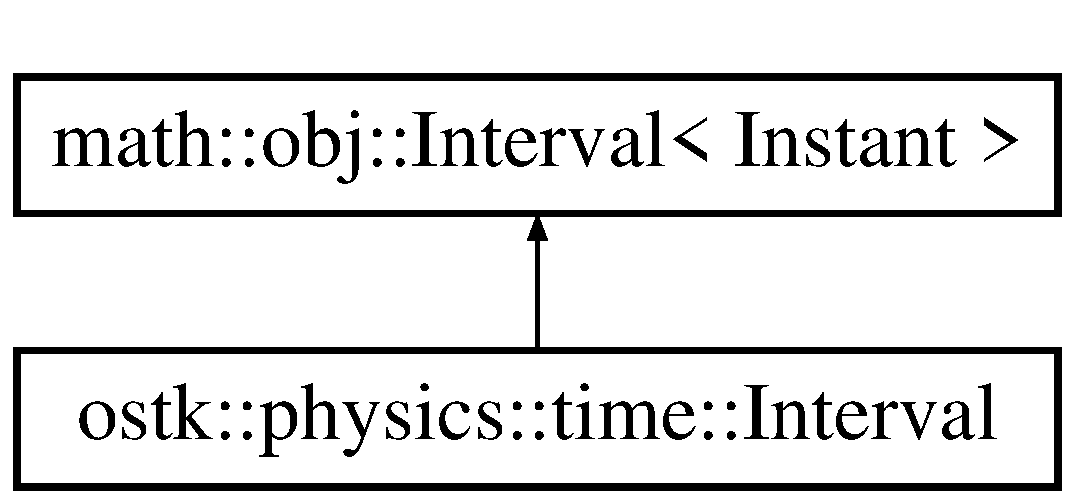
\includegraphics[height=2.000000cm]{classostk_1_1physics_1_1time_1_1_interval}
\end{center}
\end{figure}
\subsection*{Public Types}
\begin{DoxyCompactItemize}
\item 
typedef math\+::obj\+::\+Interval$<$ \hyperlink{classostk_1_1physics_1_1time_1_1_instant}{Instant} $>$\+::\hyperlink{classostk_1_1physics_1_1time_1_1_interval_a7011137ee6d84ebb8705c95d88f87818}{Type} \hyperlink{classostk_1_1physics_1_1time_1_1_interval_a7011137ee6d84ebb8705c95d88f87818}{Type}
\end{DoxyCompactItemize}
\subsection*{Public Member Functions}
\begin{DoxyCompactItemize}
\item 
\hyperlink{classostk_1_1physics_1_1time_1_1_interval_a62d60b1eb3c7c782d7c45e8b9c153b34}{Interval} (const \hyperlink{classostk_1_1physics_1_1time_1_1_instant}{Instant} \&a\+Lower\+Bound, const \hyperlink{classostk_1_1physics_1_1time_1_1_instant}{Instant} \&an\+Upper\+Bound, const \hyperlink{classostk_1_1physics_1_1time_1_1_interval_a7011137ee6d84ebb8705c95d88f87818}{Interval\+::\+Type} \&an\+Interval\+Type)
\begin{DoxyCompactList}\small\item\em Constructor. \end{DoxyCompactList}\item 
bool \hyperlink{classostk_1_1physics_1_1time_1_1_interval_aa0ed88bea385d6afddaecc3423dd87d1}{is\+Defined} () const
\item 
const \hyperlink{classostk_1_1physics_1_1time_1_1_instant}{Instant} \& \hyperlink{classostk_1_1physics_1_1time_1_1_interval_abd9702e2a12cb6d6e3e4f51c210d0af1}{access\+Start} () const
\item 
const \hyperlink{classostk_1_1physics_1_1time_1_1_instant}{Instant} \& \hyperlink{classostk_1_1physics_1_1time_1_1_interval_a1a047369c0aac66fc28e0cb09870f1d2}{access\+End} () const
\item 
\hyperlink{classostk_1_1physics_1_1time_1_1_instant}{Instant} \hyperlink{classostk_1_1physics_1_1time_1_1_interval_ab3580768bc1def986b5e55659e7d6274}{get\+Start} () const
\item 
\hyperlink{classostk_1_1physics_1_1time_1_1_instant}{Instant} \hyperlink{classostk_1_1physics_1_1time_1_1_interval_a3a1fe4fdb656d7b38ddfcefac6c620ab}{get\+End} () const
\item 
\hyperlink{classostk_1_1physics_1_1time_1_1_duration}{Duration} \hyperlink{classostk_1_1physics_1_1time_1_1_interval_ae31a3fab2f4fa2f4881df6e62b8b3aeb}{get\+Duration} () const
\item 
\hyperlink{classostk_1_1physics_1_1time_1_1_instant}{Instant} \hyperlink{classostk_1_1physics_1_1time_1_1_interval_ab0abf8d0aaf5bb6181ddda58de5fe9a2}{get\+Center} () const
\item 
String \hyperlink{classostk_1_1physics_1_1time_1_1_interval_a23ff5318aa1847ac42dc347ef509fa5a}{to\+String} (const \hyperlink{namespaceostk_1_1physics_1_1time_adf23d37bd8641fb76a0e98ab46a70df7}{Scale} \&a\+Time\+Scale=\hyperlink{namespaceostk_1_1physics_1_1time_adf23d37bd8641fb76a0e98ab46a70df7a9234324ddf6b4176b57d803a925b7961}{Scale\+::\+U\+TC}) const
\item 
Array$<$ \hyperlink{classostk_1_1physics_1_1time_1_1_instant}{Instant} $>$ \hyperlink{classostk_1_1physics_1_1time_1_1_interval_ae50bd06e26fbee080424f7d202c6cdfc}{generate\+Grid} (const \hyperlink{classostk_1_1physics_1_1time_1_1_duration}{Duration} \&a\+Time\+Step) const
\end{DoxyCompactItemize}
\subsection*{Static Public Member Functions}
\begin{DoxyCompactItemize}
\item 
static \hyperlink{classostk_1_1physics_1_1time_1_1_interval}{Interval} \hyperlink{classostk_1_1physics_1_1time_1_1_interval_a59ab818046b079fa047a739886d72747}{Undefined} ()
\item 
static \hyperlink{classostk_1_1physics_1_1time_1_1_interval}{Interval} \hyperlink{classostk_1_1physics_1_1time_1_1_interval_aa8d39973df40ac95b27cc460e86e3aa7}{Closed} (const \hyperlink{classostk_1_1physics_1_1time_1_1_instant}{Instant} \&a\+Lower\+Bound, const \hyperlink{classostk_1_1physics_1_1time_1_1_instant}{Instant} \&an\+Upper\+Bound)
\begin{DoxyCompactList}\small\item\em Constructs a closed interval. \end{DoxyCompactList}\item 
static \hyperlink{classostk_1_1physics_1_1time_1_1_interval}{Interval} \hyperlink{classostk_1_1physics_1_1time_1_1_interval_aad7763c91cd880c3a90127d1b147a0fa}{Centered} (const \hyperlink{classostk_1_1physics_1_1time_1_1_instant}{Instant} \&a\+Central\+Instant, const \hyperlink{classostk_1_1physics_1_1time_1_1_duration}{Duration} \&a\+Duration, const \hyperlink{classostk_1_1physics_1_1time_1_1_interval_a7011137ee6d84ebb8705c95d88f87818}{Interval\+::\+Type} \&an\+Interval\+Type)
\item 
static \hyperlink{classostk_1_1physics_1_1time_1_1_interval}{Interval} \hyperlink{classostk_1_1physics_1_1time_1_1_interval_a7905daf5c50e500e5450d56040dc57f4}{Parse} (const String \&a\+String)
\begin{DoxyCompactList}\small\item\em Constructs an interval from a string representation. \end{DoxyCompactList}\end{DoxyCompactItemize}
\subsection*{Friends}
\begin{DoxyCompactItemize}
\item 
std\+::ostream \& \hyperlink{classostk_1_1physics_1_1time_1_1_interval_a4671ce6746f99155561a1bdfade9749a}{operator$<$$<$} (std\+::ostream \&an\+Output\+Stream, const \hyperlink{classostk_1_1physics_1_1time_1_1_interval}{Interval} \&an\+Interval)
\end{DoxyCompactItemize}


\subsection{Detailed Description}
\hyperlink{classostk_1_1physics_1_1time_1_1_interval}{Interval}. 

\subsection{Member Typedef Documentation}
\mbox{\Hypertarget{classostk_1_1physics_1_1time_1_1_interval_a7011137ee6d84ebb8705c95d88f87818}\label{classostk_1_1physics_1_1time_1_1_interval_a7011137ee6d84ebb8705c95d88f87818}} 
\index{ostk\+::physics\+::time\+::\+Interval@{ostk\+::physics\+::time\+::\+Interval}!Type@{Type}}
\index{Type@{Type}!ostk\+::physics\+::time\+::\+Interval@{ostk\+::physics\+::time\+::\+Interval}}
\subsubsection{\texorpdfstring{Type}{Type}}
{\footnotesize\ttfamily typedef math\+::obj\+::\+Interval$<$\hyperlink{classostk_1_1physics_1_1time_1_1_instant}{Instant}$>$\+::\hyperlink{classostk_1_1physics_1_1time_1_1_interval_a7011137ee6d84ebb8705c95d88f87818}{Type} \hyperlink{classostk_1_1physics_1_1time_1_1_interval_a7011137ee6d84ebb8705c95d88f87818}{ostk\+::physics\+::time\+::\+Interval\+::\+Type}}



\subsection{Constructor \& Destructor Documentation}
\mbox{\Hypertarget{classostk_1_1physics_1_1time_1_1_interval_a62d60b1eb3c7c782d7c45e8b9c153b34}\label{classostk_1_1physics_1_1time_1_1_interval_a62d60b1eb3c7c782d7c45e8b9c153b34}} 
\index{ostk\+::physics\+::time\+::\+Interval@{ostk\+::physics\+::time\+::\+Interval}!Interval@{Interval}}
\index{Interval@{Interval}!ostk\+::physics\+::time\+::\+Interval@{ostk\+::physics\+::time\+::\+Interval}}
\subsubsection{\texorpdfstring{Interval()}{Interval()}}
{\footnotesize\ttfamily ostk\+::physics\+::time\+::\+Interval\+::\+Interval (\begin{DoxyParamCaption}\item[{const \hyperlink{classostk_1_1physics_1_1time_1_1_instant}{Instant} \&}]{a\+Lower\+Bound,  }\item[{const \hyperlink{classostk_1_1physics_1_1time_1_1_instant}{Instant} \&}]{an\+Upper\+Bound,  }\item[{const \hyperlink{classostk_1_1physics_1_1time_1_1_interval_a7011137ee6d84ebb8705c95d88f87818}{Interval\+::\+Type} \&}]{an\+Interval\+Type }\end{DoxyParamCaption})}



Constructor. 


\begin{DoxyCode}
\hyperlink{classostk_1_1physics_1_1time_1_1_interval_a62d60b1eb3c7c782d7c45e8b9c153b34}{Interval} interval(\hyperlink{classostk_1_1physics_1_1time_1_1_instant_a3f84d0c2d0b140326d3b172b54e3ffff}{Instant::J2000}(), \hyperlink{classostk_1_1physics_1_1time_1_1_instant_afbc9a9219aa94e8a828f5876ee68f42c}{Instant::Now}(), 
      Interval::Type::Closed) ;
\end{DoxyCode}



\begin{DoxyParams}[1]{Parameters}
\mbox{\tt in}  & {\em a\+Lower\+Bound} & A lower bound \\
\hline
\mbox{\tt in}  & {\em an\+Upper\+Bound} & An upper bound \\
\hline
\mbox{\tt in}  & {\em an\+Interval\+Type} & An interval type \\
\hline
\end{DoxyParams}


\subsection{Member Function Documentation}
\mbox{\Hypertarget{classostk_1_1physics_1_1time_1_1_interval_a1a047369c0aac66fc28e0cb09870f1d2}\label{classostk_1_1physics_1_1time_1_1_interval_a1a047369c0aac66fc28e0cb09870f1d2}} 
\index{ostk\+::physics\+::time\+::\+Interval@{ostk\+::physics\+::time\+::\+Interval}!access\+End@{access\+End}}
\index{access\+End@{access\+End}!ostk\+::physics\+::time\+::\+Interval@{ostk\+::physics\+::time\+::\+Interval}}
\subsubsection{\texorpdfstring{access\+End()}{accessEnd()}}
{\footnotesize\ttfamily const \hyperlink{classostk_1_1physics_1_1time_1_1_instant}{Instant} \& ostk\+::physics\+::time\+::\+Interval\+::access\+End (\begin{DoxyParamCaption}{ }\end{DoxyParamCaption}) const}

\mbox{\Hypertarget{classostk_1_1physics_1_1time_1_1_interval_abd9702e2a12cb6d6e3e4f51c210d0af1}\label{classostk_1_1physics_1_1time_1_1_interval_abd9702e2a12cb6d6e3e4f51c210d0af1}} 
\index{ostk\+::physics\+::time\+::\+Interval@{ostk\+::physics\+::time\+::\+Interval}!access\+Start@{access\+Start}}
\index{access\+Start@{access\+Start}!ostk\+::physics\+::time\+::\+Interval@{ostk\+::physics\+::time\+::\+Interval}}
\subsubsection{\texorpdfstring{access\+Start()}{accessStart()}}
{\footnotesize\ttfamily const \hyperlink{classostk_1_1physics_1_1time_1_1_instant}{Instant} \& ostk\+::physics\+::time\+::\+Interval\+::access\+Start (\begin{DoxyParamCaption}{ }\end{DoxyParamCaption}) const}

\mbox{\Hypertarget{classostk_1_1physics_1_1time_1_1_interval_aad7763c91cd880c3a90127d1b147a0fa}\label{classostk_1_1physics_1_1time_1_1_interval_aad7763c91cd880c3a90127d1b147a0fa}} 
\index{ostk\+::physics\+::time\+::\+Interval@{ostk\+::physics\+::time\+::\+Interval}!Centered@{Centered}}
\index{Centered@{Centered}!ostk\+::physics\+::time\+::\+Interval@{ostk\+::physics\+::time\+::\+Interval}}
\subsubsection{\texorpdfstring{Centered()}{Centered()}}
{\footnotesize\ttfamily \hyperlink{classostk_1_1physics_1_1time_1_1_interval}{Interval} ostk\+::physics\+::time\+::\+Interval\+::\+Centered (\begin{DoxyParamCaption}\item[{const \hyperlink{classostk_1_1physics_1_1time_1_1_instant}{Instant} \&}]{a\+Central\+Instant,  }\item[{const \hyperlink{classostk_1_1physics_1_1time_1_1_duration}{Duration} \&}]{a\+Duration,  }\item[{const \hyperlink{classostk_1_1physics_1_1time_1_1_interval_a7011137ee6d84ebb8705c95d88f87818}{Interval\+::\+Type} \&}]{an\+Interval\+Type }\end{DoxyParamCaption})\hspace{0.3cm}{\ttfamily [static]}}

\mbox{\Hypertarget{classostk_1_1physics_1_1time_1_1_interval_aa8d39973df40ac95b27cc460e86e3aa7}\label{classostk_1_1physics_1_1time_1_1_interval_aa8d39973df40ac95b27cc460e86e3aa7}} 
\index{ostk\+::physics\+::time\+::\+Interval@{ostk\+::physics\+::time\+::\+Interval}!Closed@{Closed}}
\index{Closed@{Closed}!ostk\+::physics\+::time\+::\+Interval@{ostk\+::physics\+::time\+::\+Interval}}
\subsubsection{\texorpdfstring{Closed()}{Closed()}}
{\footnotesize\ttfamily \hyperlink{classostk_1_1physics_1_1time_1_1_interval}{Interval} ostk\+::physics\+::time\+::\+Interval\+::\+Closed (\begin{DoxyParamCaption}\item[{const \hyperlink{classostk_1_1physics_1_1time_1_1_instant}{Instant} \&}]{a\+Lower\+Bound,  }\item[{const \hyperlink{classostk_1_1physics_1_1time_1_1_instant}{Instant} \&}]{an\+Upper\+Bound }\end{DoxyParamCaption})\hspace{0.3cm}{\ttfamily [static]}}



Constructs a closed interval. 


\begin{DoxyCode}
\hyperlink{classostk_1_1physics_1_1time_1_1_interval_a62d60b1eb3c7c782d7c45e8b9c153b34}{Interval} interval = \hyperlink{classostk_1_1physics_1_1time_1_1_interval_aa8d39973df40ac95b27cc460e86e3aa7}{Interval::Closed}(\hyperlink{classostk_1_1physics_1_1time_1_1_instant_a3f84d0c2d0b140326d3b172b54e3ffff}{Instant::J2000}(), 
      \hyperlink{classostk_1_1physics_1_1time_1_1_instant_afbc9a9219aa94e8a828f5876ee68f42c}{Instant::Now}()) ; \textcolor{comment}{// [J2000, Now]}
\end{DoxyCode}


\begin{DoxyReturn}{Returns}
Closed interval 
\end{DoxyReturn}
\mbox{\Hypertarget{classostk_1_1physics_1_1time_1_1_interval_ae50bd06e26fbee080424f7d202c6cdfc}\label{classostk_1_1physics_1_1time_1_1_interval_ae50bd06e26fbee080424f7d202c6cdfc}} 
\index{ostk\+::physics\+::time\+::\+Interval@{ostk\+::physics\+::time\+::\+Interval}!generate\+Grid@{generate\+Grid}}
\index{generate\+Grid@{generate\+Grid}!ostk\+::physics\+::time\+::\+Interval@{ostk\+::physics\+::time\+::\+Interval}}
\subsubsection{\texorpdfstring{generate\+Grid()}{generateGrid()}}
{\footnotesize\ttfamily Array$<$ \hyperlink{classostk_1_1physics_1_1time_1_1_instant}{Instant} $>$ ostk\+::physics\+::time\+::\+Interval\+::generate\+Grid (\begin{DoxyParamCaption}\item[{const \hyperlink{classostk_1_1physics_1_1time_1_1_duration}{Duration} \&}]{a\+Time\+Step }\end{DoxyParamCaption}) const}

\mbox{\Hypertarget{classostk_1_1physics_1_1time_1_1_interval_ab0abf8d0aaf5bb6181ddda58de5fe9a2}\label{classostk_1_1physics_1_1time_1_1_interval_ab0abf8d0aaf5bb6181ddda58de5fe9a2}} 
\index{ostk\+::physics\+::time\+::\+Interval@{ostk\+::physics\+::time\+::\+Interval}!get\+Center@{get\+Center}}
\index{get\+Center@{get\+Center}!ostk\+::physics\+::time\+::\+Interval@{ostk\+::physics\+::time\+::\+Interval}}
\subsubsection{\texorpdfstring{get\+Center()}{getCenter()}}
{\footnotesize\ttfamily \hyperlink{classostk_1_1physics_1_1time_1_1_instant}{Instant} ostk\+::physics\+::time\+::\+Interval\+::get\+Center (\begin{DoxyParamCaption}{ }\end{DoxyParamCaption}) const}

\mbox{\Hypertarget{classostk_1_1physics_1_1time_1_1_interval_ae31a3fab2f4fa2f4881df6e62b8b3aeb}\label{classostk_1_1physics_1_1time_1_1_interval_ae31a3fab2f4fa2f4881df6e62b8b3aeb}} 
\index{ostk\+::physics\+::time\+::\+Interval@{ostk\+::physics\+::time\+::\+Interval}!get\+Duration@{get\+Duration}}
\index{get\+Duration@{get\+Duration}!ostk\+::physics\+::time\+::\+Interval@{ostk\+::physics\+::time\+::\+Interval}}
\subsubsection{\texorpdfstring{get\+Duration()}{getDuration()}}
{\footnotesize\ttfamily \hyperlink{classostk_1_1physics_1_1time_1_1_duration}{Duration} ostk\+::physics\+::time\+::\+Interval\+::get\+Duration (\begin{DoxyParamCaption}{ }\end{DoxyParamCaption}) const}

\mbox{\Hypertarget{classostk_1_1physics_1_1time_1_1_interval_a3a1fe4fdb656d7b38ddfcefac6c620ab}\label{classostk_1_1physics_1_1time_1_1_interval_a3a1fe4fdb656d7b38ddfcefac6c620ab}} 
\index{ostk\+::physics\+::time\+::\+Interval@{ostk\+::physics\+::time\+::\+Interval}!get\+End@{get\+End}}
\index{get\+End@{get\+End}!ostk\+::physics\+::time\+::\+Interval@{ostk\+::physics\+::time\+::\+Interval}}
\subsubsection{\texorpdfstring{get\+End()}{getEnd()}}
{\footnotesize\ttfamily \hyperlink{classostk_1_1physics_1_1time_1_1_instant}{Instant} ostk\+::physics\+::time\+::\+Interval\+::get\+End (\begin{DoxyParamCaption}{ }\end{DoxyParamCaption}) const}

\mbox{\Hypertarget{classostk_1_1physics_1_1time_1_1_interval_ab3580768bc1def986b5e55659e7d6274}\label{classostk_1_1physics_1_1time_1_1_interval_ab3580768bc1def986b5e55659e7d6274}} 
\index{ostk\+::physics\+::time\+::\+Interval@{ostk\+::physics\+::time\+::\+Interval}!get\+Start@{get\+Start}}
\index{get\+Start@{get\+Start}!ostk\+::physics\+::time\+::\+Interval@{ostk\+::physics\+::time\+::\+Interval}}
\subsubsection{\texorpdfstring{get\+Start()}{getStart()}}
{\footnotesize\ttfamily \hyperlink{classostk_1_1physics_1_1time_1_1_instant}{Instant} ostk\+::physics\+::time\+::\+Interval\+::get\+Start (\begin{DoxyParamCaption}{ }\end{DoxyParamCaption}) const}

\mbox{\Hypertarget{classostk_1_1physics_1_1time_1_1_interval_aa0ed88bea385d6afddaecc3423dd87d1}\label{classostk_1_1physics_1_1time_1_1_interval_aa0ed88bea385d6afddaecc3423dd87d1}} 
\index{ostk\+::physics\+::time\+::\+Interval@{ostk\+::physics\+::time\+::\+Interval}!is\+Defined@{is\+Defined}}
\index{is\+Defined@{is\+Defined}!ostk\+::physics\+::time\+::\+Interval@{ostk\+::physics\+::time\+::\+Interval}}
\subsubsection{\texorpdfstring{is\+Defined()}{isDefined()}}
{\footnotesize\ttfamily bool ostk\+::physics\+::time\+::\+Interval\+::is\+Defined (\begin{DoxyParamCaption}{ }\end{DoxyParamCaption}) const}

\mbox{\Hypertarget{classostk_1_1physics_1_1time_1_1_interval_a7905daf5c50e500e5450d56040dc57f4}\label{classostk_1_1physics_1_1time_1_1_interval_a7905daf5c50e500e5450d56040dc57f4}} 
\index{ostk\+::physics\+::time\+::\+Interval@{ostk\+::physics\+::time\+::\+Interval}!Parse@{Parse}}
\index{Parse@{Parse}!ostk\+::physics\+::time\+::\+Interval@{ostk\+::physics\+::time\+::\+Interval}}
\subsubsection{\texorpdfstring{Parse()}{Parse()}}
{\footnotesize\ttfamily \hyperlink{classostk_1_1physics_1_1time_1_1_interval}{Interval} ostk\+::physics\+::time\+::\+Interval\+::\+Parse (\begin{DoxyParamCaption}\item[{const String \&}]{a\+String }\end{DoxyParamCaption})\hspace{0.3cm}{\ttfamily [static]}}



Constructs an interval from a string representation. 


\begin{DoxyCode}
...
\end{DoxyCode}



\begin{DoxyParams}[1]{Parameters}
\mbox{\tt in}  & {\em a\+String} & A string \\
\hline
\end{DoxyParams}
\begin{DoxyReturn}{Returns}
\hyperlink{classostk_1_1physics_1_1time_1_1_interval}{Interval} 
\end{DoxyReturn}
\mbox{\Hypertarget{classostk_1_1physics_1_1time_1_1_interval_a23ff5318aa1847ac42dc347ef509fa5a}\label{classostk_1_1physics_1_1time_1_1_interval_a23ff5318aa1847ac42dc347ef509fa5a}} 
\index{ostk\+::physics\+::time\+::\+Interval@{ostk\+::physics\+::time\+::\+Interval}!to\+String@{to\+String}}
\index{to\+String@{to\+String}!ostk\+::physics\+::time\+::\+Interval@{ostk\+::physics\+::time\+::\+Interval}}
\subsubsection{\texorpdfstring{to\+String()}{toString()}}
{\footnotesize\ttfamily String ostk\+::physics\+::time\+::\+Interval\+::to\+String (\begin{DoxyParamCaption}\item[{const \hyperlink{namespaceostk_1_1physics_1_1time_adf23d37bd8641fb76a0e98ab46a70df7}{Scale} \&}]{a\+Time\+Scale = {\ttfamily \hyperlink{namespaceostk_1_1physics_1_1time_adf23d37bd8641fb76a0e98ab46a70df7a9234324ddf6b4176b57d803a925b7961}{Scale\+::\+U\+TC}} }\end{DoxyParamCaption}) const}

\mbox{\Hypertarget{classostk_1_1physics_1_1time_1_1_interval_a59ab818046b079fa047a739886d72747}\label{classostk_1_1physics_1_1time_1_1_interval_a59ab818046b079fa047a739886d72747}} 
\index{ostk\+::physics\+::time\+::\+Interval@{ostk\+::physics\+::time\+::\+Interval}!Undefined@{Undefined}}
\index{Undefined@{Undefined}!ostk\+::physics\+::time\+::\+Interval@{ostk\+::physics\+::time\+::\+Interval}}
\subsubsection{\texorpdfstring{Undefined()}{Undefined()}}
{\footnotesize\ttfamily \hyperlink{classostk_1_1physics_1_1time_1_1_interval}{Interval} ostk\+::physics\+::time\+::\+Interval\+::\+Undefined (\begin{DoxyParamCaption}{ }\end{DoxyParamCaption})\hspace{0.3cm}{\ttfamily [static]}}



\subsection{Friends And Related Function Documentation}
\mbox{\Hypertarget{classostk_1_1physics_1_1time_1_1_interval_a4671ce6746f99155561a1bdfade9749a}\label{classostk_1_1physics_1_1time_1_1_interval_a4671ce6746f99155561a1bdfade9749a}} 
\index{ostk\+::physics\+::time\+::\+Interval@{ostk\+::physics\+::time\+::\+Interval}!operator$<$$<$@{operator$<$$<$}}
\index{operator$<$$<$@{operator$<$$<$}!ostk\+::physics\+::time\+::\+Interval@{ostk\+::physics\+::time\+::\+Interval}}
\subsubsection{\texorpdfstring{operator$<$$<$}{operator<<}}
{\footnotesize\ttfamily std\+::ostream\& operator$<$$<$ (\begin{DoxyParamCaption}\item[{std\+::ostream \&}]{an\+Output\+Stream,  }\item[{const \hyperlink{classostk_1_1physics_1_1time_1_1_interval}{Interval} \&}]{an\+Interval }\end{DoxyParamCaption})\hspace{0.3cm}{\ttfamily [friend]}}



The documentation for this class was generated from the following files\+:\begin{DoxyCompactItemize}
\item 
include/\+Open\+Space\+Toolkit/\+Physics/\+Time/\hyperlink{_interval_8hpp}{Interval.\+hpp}\item 
src/\+Open\+Space\+Toolkit/\+Physics/\+Time/\hyperlink{_interval_8cpp}{Interval.\+cpp}\end{DoxyCompactItemize}

\hypertarget{classostk_1_1physics_1_1coord_1_1frame_1_1provider_1_1_i_t_r_f}{}\section{ostk\+:\+:physics\+:\+:coord\+:\+:frame\+:\+:provider\+:\+:I\+T\+RF Class Reference}
\label{classostk_1_1physics_1_1coord_1_1frame_1_1provider_1_1_i_t_r_f}\index{ostk\+::physics\+::coord\+::frame\+::provider\+::\+I\+T\+RF@{ostk\+::physics\+::coord\+::frame\+::provider\+::\+I\+T\+RF}}


International Terrestrial Reference System (\hyperlink{classostk_1_1physics_1_1coord_1_1frame_1_1provider_1_1_i_t_r_f}{I\+T\+RF}) provider.  




{\ttfamily \#include $<$I\+T\+R\+F.\+hpp$>$}

Inheritance diagram for ostk\+:\+:physics\+:\+:coord\+:\+:frame\+:\+:provider\+:\+:I\+T\+RF\+:\begin{figure}[H]
\begin{center}
\leavevmode
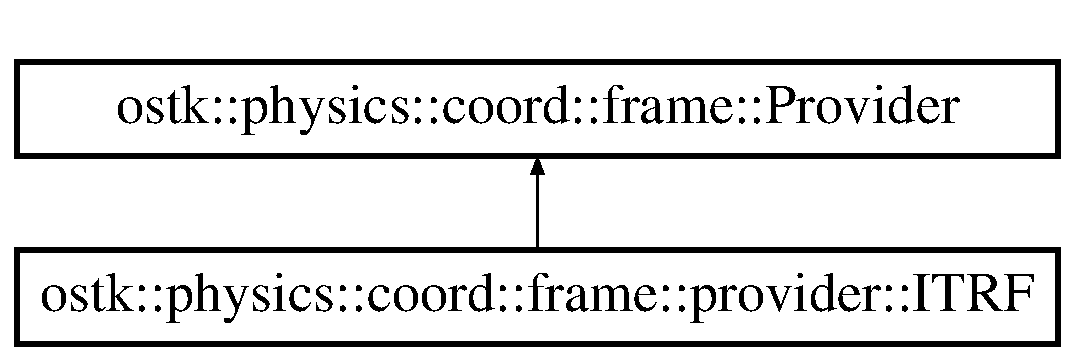
\includegraphics[height=2.000000cm]{classostk_1_1physics_1_1coord_1_1frame_1_1provider_1_1_i_t_r_f}
\end{center}
\end{figure}
\subsection*{Public Member Functions}
\begin{DoxyCompactItemize}
\item 
\hyperlink{classostk_1_1physics_1_1coord_1_1frame_1_1provider_1_1_i_t_r_f_a8b1ca7dc9e763e927263bb1b57237208}{I\+T\+RF} ()
\item 
virtual \hyperlink{classostk_1_1physics_1_1coord_1_1frame_1_1provider_1_1_i_t_r_f_a70c48b2f1f9816a858144d8dde762b5d}{$\sim$\+I\+T\+RF} () override
\item 
virtual \hyperlink{classostk_1_1physics_1_1coord_1_1frame_1_1provider_1_1_i_t_r_f}{I\+T\+RF} $\ast$ \hyperlink{classostk_1_1physics_1_1coord_1_1frame_1_1provider_1_1_i_t_r_f_aad7e29329b68f264bed571bf48b902a4}{clone} () const override
\item 
virtual bool \hyperlink{classostk_1_1physics_1_1coord_1_1frame_1_1provider_1_1_i_t_r_f_a2f3a53b002d54f1adf829cefc2cf7393}{is\+Defined} () const override
\item 
virtual \hyperlink{classostk_1_1physics_1_1coord_1_1_transform}{Transform} \hyperlink{classostk_1_1physics_1_1coord_1_1frame_1_1provider_1_1_i_t_r_f_a6e344e7252a962d4451e2c0ea866bc30}{get\+Transform\+At} (const \hyperlink{classostk_1_1physics_1_1time_1_1_instant}{Instant} \&an\+Instant) const override
\end{DoxyCompactItemize}


\subsection{Detailed Description}
International Terrestrial Reference System (\hyperlink{classostk_1_1physics_1_1coord_1_1frame_1_1provider_1_1_i_t_r_f}{I\+T\+RF}) provider. 

https\+://en.wikipedia.\+org/wiki/\+International\+\_\+\+Terrestrial\+\_\+\+Reference\+\_\+\+System 

\subsection{Constructor \& Destructor Documentation}
\mbox{\Hypertarget{classostk_1_1physics_1_1coord_1_1frame_1_1provider_1_1_i_t_r_f_a8b1ca7dc9e763e927263bb1b57237208}\label{classostk_1_1physics_1_1coord_1_1frame_1_1provider_1_1_i_t_r_f_a8b1ca7dc9e763e927263bb1b57237208}} 
\index{ostk\+::physics\+::coord\+::frame\+::provider\+::\+I\+T\+RF@{ostk\+::physics\+::coord\+::frame\+::provider\+::\+I\+T\+RF}!I\+T\+RF@{I\+T\+RF}}
\index{I\+T\+RF@{I\+T\+RF}!ostk\+::physics\+::coord\+::frame\+::provider\+::\+I\+T\+RF@{ostk\+::physics\+::coord\+::frame\+::provider\+::\+I\+T\+RF}}
\subsubsection{\texorpdfstring{I\+T\+R\+F()}{ITRF()}}
{\footnotesize\ttfamily ostk\+::physics\+::coord\+::frame\+::provider\+::\+I\+T\+R\+F\+::\+I\+T\+RF (\begin{DoxyParamCaption}{ }\end{DoxyParamCaption})}

\mbox{\Hypertarget{classostk_1_1physics_1_1coord_1_1frame_1_1provider_1_1_i_t_r_f_a70c48b2f1f9816a858144d8dde762b5d}\label{classostk_1_1physics_1_1coord_1_1frame_1_1provider_1_1_i_t_r_f_a70c48b2f1f9816a858144d8dde762b5d}} 
\index{ostk\+::physics\+::coord\+::frame\+::provider\+::\+I\+T\+RF@{ostk\+::physics\+::coord\+::frame\+::provider\+::\+I\+T\+RF}!````~I\+T\+RF@{$\sim$\+I\+T\+RF}}
\index{````~I\+T\+RF@{$\sim$\+I\+T\+RF}!ostk\+::physics\+::coord\+::frame\+::provider\+::\+I\+T\+RF@{ostk\+::physics\+::coord\+::frame\+::provider\+::\+I\+T\+RF}}
\subsubsection{\texorpdfstring{$\sim$\+I\+T\+R\+F()}{~ITRF()}}
{\footnotesize\ttfamily ostk\+::physics\+::coord\+::frame\+::provider\+::\+I\+T\+R\+F\+::$\sim$\+I\+T\+RF (\begin{DoxyParamCaption}{ }\end{DoxyParamCaption})\hspace{0.3cm}{\ttfamily [override]}, {\ttfamily [virtual]}}



\subsection{Member Function Documentation}
\mbox{\Hypertarget{classostk_1_1physics_1_1coord_1_1frame_1_1provider_1_1_i_t_r_f_aad7e29329b68f264bed571bf48b902a4}\label{classostk_1_1physics_1_1coord_1_1frame_1_1provider_1_1_i_t_r_f_aad7e29329b68f264bed571bf48b902a4}} 
\index{ostk\+::physics\+::coord\+::frame\+::provider\+::\+I\+T\+RF@{ostk\+::physics\+::coord\+::frame\+::provider\+::\+I\+T\+RF}!clone@{clone}}
\index{clone@{clone}!ostk\+::physics\+::coord\+::frame\+::provider\+::\+I\+T\+RF@{ostk\+::physics\+::coord\+::frame\+::provider\+::\+I\+T\+RF}}
\subsubsection{\texorpdfstring{clone()}{clone()}}
{\footnotesize\ttfamily \hyperlink{classostk_1_1physics_1_1coord_1_1frame_1_1provider_1_1_i_t_r_f}{I\+T\+RF} $\ast$ ostk\+::physics\+::coord\+::frame\+::provider\+::\+I\+T\+R\+F\+::clone (\begin{DoxyParamCaption}{ }\end{DoxyParamCaption}) const\hspace{0.3cm}{\ttfamily [override]}, {\ttfamily [virtual]}}



Implements \hyperlink{classostk_1_1physics_1_1coord_1_1frame_1_1_provider_ae41bc3862d088e9c8d90a79253294ce9}{ostk\+::physics\+::coord\+::frame\+::\+Provider}.

\mbox{\Hypertarget{classostk_1_1physics_1_1coord_1_1frame_1_1provider_1_1_i_t_r_f_a6e344e7252a962d4451e2c0ea866bc30}\label{classostk_1_1physics_1_1coord_1_1frame_1_1provider_1_1_i_t_r_f_a6e344e7252a962d4451e2c0ea866bc30}} 
\index{ostk\+::physics\+::coord\+::frame\+::provider\+::\+I\+T\+RF@{ostk\+::physics\+::coord\+::frame\+::provider\+::\+I\+T\+RF}!get\+Transform\+At@{get\+Transform\+At}}
\index{get\+Transform\+At@{get\+Transform\+At}!ostk\+::physics\+::coord\+::frame\+::provider\+::\+I\+T\+RF@{ostk\+::physics\+::coord\+::frame\+::provider\+::\+I\+T\+RF}}
\subsubsection{\texorpdfstring{get\+Transform\+At()}{getTransformAt()}}
{\footnotesize\ttfamily \hyperlink{classostk_1_1physics_1_1coord_1_1_transform}{Transform} ostk\+::physics\+::coord\+::frame\+::provider\+::\+I\+T\+R\+F\+::get\+Transform\+At (\begin{DoxyParamCaption}\item[{const \hyperlink{classostk_1_1physics_1_1time_1_1_instant}{Instant} \&}]{an\+Instant }\end{DoxyParamCaption}) const\hspace{0.3cm}{\ttfamily [override]}, {\ttfamily [virtual]}}



Implements \hyperlink{classostk_1_1physics_1_1coord_1_1frame_1_1_provider_a38b86a589f46f8b8a9c97ab2776f37d1}{ostk\+::physics\+::coord\+::frame\+::\+Provider}.

\mbox{\Hypertarget{classostk_1_1physics_1_1coord_1_1frame_1_1provider_1_1_i_t_r_f_a2f3a53b002d54f1adf829cefc2cf7393}\label{classostk_1_1physics_1_1coord_1_1frame_1_1provider_1_1_i_t_r_f_a2f3a53b002d54f1adf829cefc2cf7393}} 
\index{ostk\+::physics\+::coord\+::frame\+::provider\+::\+I\+T\+RF@{ostk\+::physics\+::coord\+::frame\+::provider\+::\+I\+T\+RF}!is\+Defined@{is\+Defined}}
\index{is\+Defined@{is\+Defined}!ostk\+::physics\+::coord\+::frame\+::provider\+::\+I\+T\+RF@{ostk\+::physics\+::coord\+::frame\+::provider\+::\+I\+T\+RF}}
\subsubsection{\texorpdfstring{is\+Defined()}{isDefined()}}
{\footnotesize\ttfamily bool ostk\+::physics\+::coord\+::frame\+::provider\+::\+I\+T\+R\+F\+::is\+Defined (\begin{DoxyParamCaption}{ }\end{DoxyParamCaption}) const\hspace{0.3cm}{\ttfamily [override]}, {\ttfamily [virtual]}}



Implements \hyperlink{classostk_1_1physics_1_1coord_1_1frame_1_1_provider_a27acab0012649796b97956fed1a91493}{ostk\+::physics\+::coord\+::frame\+::\+Provider}.



The documentation for this class was generated from the following files\+:\begin{DoxyCompactItemize}
\item 
include/\+Open\+Space\+Toolkit/\+Physics/\+Coordinate/\+Frame/\+Providers/\hyperlink{_i_t_r_f_8hpp}{I\+T\+R\+F.\+hpp}\item 
src/\+Open\+Space\+Toolkit/\+Physics/\+Coordinate/\+Frame/\+Providers/\hyperlink{_i_t_r_f_8cpp}{I\+T\+R\+F.\+cpp}\end{DoxyCompactItemize}

\hypertarget{classostk_1_1physics_1_1env_1_1ephem_1_1spice_1_1_kernel}{}\section{ostk\+:\+:physics\+:\+:env\+:\+:ephem\+:\+:spice\+:\+:Kernel Class Reference}
\label{classostk_1_1physics_1_1env_1_1ephem_1_1spice_1_1_kernel}\index{ostk\+::physics\+::env\+::ephem\+::spice\+::\+Kernel@{ostk\+::physics\+::env\+::ephem\+::spice\+::\+Kernel}}


\hyperlink{classostk_1_1physics_1_1env_1_1ephem_1_1_s_p_i_c_e}{S\+P\+I\+CE} Toolkit kernel.  




{\ttfamily \#include $<$Kernel.\+hpp$>$}

\subsection*{Public Types}
\begin{DoxyCompactItemize}
\item 
enum \hyperlink{classostk_1_1physics_1_1env_1_1ephem_1_1spice_1_1_kernel_a76d560bbface15a0cb24cd82e9a93d77}{Type} \{ \newline
\hyperlink{classostk_1_1physics_1_1env_1_1ephem_1_1spice_1_1_kernel_a76d560bbface15a0cb24cd82e9a93d77aec0fc0100c4fc1ce4eea230c3dc10360}{Type\+::\+Undefined}, 
\hyperlink{classostk_1_1physics_1_1env_1_1ephem_1_1spice_1_1_kernel_a76d560bbface15a0cb24cd82e9a93d77ae5ebe7b9d4b13b67cb85ac2febe4aca2}{Type\+::\+S\+C\+LK}, 
\hyperlink{classostk_1_1physics_1_1env_1_1ephem_1_1spice_1_1_kernel_a76d560bbface15a0cb24cd82e9a93d77a1352b10452a6331f4858173133cad49d}{Type\+::\+L\+SK}, 
\hyperlink{classostk_1_1physics_1_1env_1_1ephem_1_1spice_1_1_kernel_a76d560bbface15a0cb24cd82e9a93d77abed028f19aa93adb7f45e064155e5278}{Type\+::\+P\+CK}, 
\newline
\hyperlink{classostk_1_1physics_1_1env_1_1ephem_1_1spice_1_1_kernel_a76d560bbface15a0cb24cd82e9a93d77a7ab2200d24b19f1824cef3f53b5b69ca}{Type\+::\+IK}, 
\hyperlink{classostk_1_1physics_1_1env_1_1ephem_1_1spice_1_1_kernel_a76d560bbface15a0cb24cd82e9a93d77a8c8ba29dafd95af91e280d1e80b81773}{Type\+::\+FK}, 
\hyperlink{classostk_1_1physics_1_1env_1_1ephem_1_1spice_1_1_kernel_a76d560bbface15a0cb24cd82e9a93d77a6aa451b53d492a8f5a2fa1fa2855be8b}{Type\+::\+EK}, 
\hyperlink{classostk_1_1physics_1_1env_1_1ephem_1_1spice_1_1_kernel_a76d560bbface15a0cb24cd82e9a93d77afbd1e7ba9564863b88d5c43cb833afaf}{Type\+::\+MK}, 
\newline
\hyperlink{classostk_1_1physics_1_1env_1_1ephem_1_1spice_1_1_kernel_a76d560bbface15a0cb24cd82e9a93d77aa77fe9806504467c944718a3ce1ed5cb}{Type\+::\+S\+PK}, 
\hyperlink{classostk_1_1physics_1_1env_1_1ephem_1_1spice_1_1_kernel_a76d560bbface15a0cb24cd82e9a93d77a357e2ff99b2ce7d86f78fca1353088ec}{Type\+::\+B\+P\+CK}, 
\hyperlink{classostk_1_1physics_1_1env_1_1ephem_1_1spice_1_1_kernel_a76d560bbface15a0cb24cd82e9a93d77a534ac75c2e8ac3e3fe7bc32bb8c6e34a}{Type\+::\+CK}, 
\hyperlink{classostk_1_1physics_1_1env_1_1ephem_1_1spice_1_1_kernel_a76d560bbface15a0cb24cd82e9a93d77a23d71b8d68c6f4869b29ed158e97c88a}{Type\+::\+B\+EK}
 \}
\end{DoxyCompactItemize}
\subsection*{Public Member Functions}
\begin{DoxyCompactItemize}
\item 
\hyperlink{classostk_1_1physics_1_1env_1_1ephem_1_1spice_1_1_kernel_afba440f0d5553591d9217c2a5e7035b5}{Kernel} (const \hyperlink{classostk_1_1physics_1_1env_1_1ephem_1_1spice_1_1_kernel_a76d560bbface15a0cb24cd82e9a93d77}{Kernel\+::\+Type} \&a\+Type, const fs\+::\+File \&a\+File)
\begin{DoxyCompactList}\small\item\em Constructor. \end{DoxyCompactList}\item 
bool \hyperlink{classostk_1_1physics_1_1env_1_1ephem_1_1spice_1_1_kernel_a4499b4c8a89b9aa99fe90bac124e89ef}{operator==} (const \hyperlink{classostk_1_1physics_1_1env_1_1ephem_1_1spice_1_1_kernel}{Kernel} \&a\+Kernel) const
\begin{DoxyCompactList}\small\item\em Equal to operator. \end{DoxyCompactList}\item 
bool \hyperlink{classostk_1_1physics_1_1env_1_1ephem_1_1spice_1_1_kernel_a1b2d11521cac8056058e774eee8082ae}{operator!=} (const \hyperlink{classostk_1_1physics_1_1env_1_1ephem_1_1spice_1_1_kernel}{Kernel} \&a\+Kernel) const
\begin{DoxyCompactList}\small\item\em Not equal to operator. \end{DoxyCompactList}\item 
bool \hyperlink{classostk_1_1physics_1_1env_1_1ephem_1_1spice_1_1_kernel_a06668d90a8b74338de4863880d362239}{is\+Defined} () const
\begin{DoxyCompactList}\small\item\em Returns true if kernel is defined. \end{DoxyCompactList}\item 
\hyperlink{classostk_1_1physics_1_1env_1_1ephem_1_1spice_1_1_kernel_a76d560bbface15a0cb24cd82e9a93d77}{Kernel\+::\+Type} \hyperlink{classostk_1_1physics_1_1env_1_1ephem_1_1spice_1_1_kernel_a4b592a8ad9e7dd8c44807b53afafaf3b}{get\+Type} () const
\begin{DoxyCompactList}\small\item\em Get kernel type. \end{DoxyCompactList}\item 
String \hyperlink{classostk_1_1physics_1_1env_1_1ephem_1_1spice_1_1_kernel_ab5029446586728c69fab3c3c6e53f5f9}{get\+Name} () const
\begin{DoxyCompactList}\small\item\em Get kernel name. \end{DoxyCompactList}\item 
fs\+::\+File \hyperlink{classostk_1_1physics_1_1env_1_1ephem_1_1spice_1_1_kernel_a8f923e5079064c8e1d79e9fe275f4b0c}{get\+File} () const
\begin{DoxyCompactList}\small\item\em Get kernel file. \end{DoxyCompactList}\end{DoxyCompactItemize}
\subsection*{Static Public Member Functions}
\begin{DoxyCompactItemize}
\item 
static \hyperlink{classostk_1_1physics_1_1env_1_1ephem_1_1spice_1_1_kernel}{Kernel} \hyperlink{classostk_1_1physics_1_1env_1_1ephem_1_1spice_1_1_kernel_adbae01d9d825d6f3863300c19d4e9645}{Undefined} ()
\begin{DoxyCompactList}\small\item\em Constructs an undefined kernel. \end{DoxyCompactList}\item 
static \hyperlink{classostk_1_1physics_1_1env_1_1ephem_1_1spice_1_1_kernel}{Kernel} \hyperlink{classostk_1_1physics_1_1env_1_1ephem_1_1spice_1_1_kernel_ac8fd10aa02653d50fb9eb32643172531}{File} (const fs\+::\+File \&a\+File)
\begin{DoxyCompactList}\small\item\em Constructs a kernel from a file. \end{DoxyCompactList}\item 
static \hyperlink{classostk_1_1physics_1_1env_1_1ephem_1_1spice_1_1_kernel_a76d560bbface15a0cb24cd82e9a93d77}{Kernel\+::\+Type} \hyperlink{classostk_1_1physics_1_1env_1_1ephem_1_1spice_1_1_kernel_a95148b8d8a008742cb09c7c5fddde8f8}{Type\+From\+String} (const String \&a\+String)
\begin{DoxyCompactList}\small\item\em Converts kernel type string to type. \end{DoxyCompactList}\item 
static String \hyperlink{classostk_1_1physics_1_1env_1_1ephem_1_1spice_1_1_kernel_a9774d27862bbc05354e30f093c666f7c}{String\+From\+Type} (const \hyperlink{classostk_1_1physics_1_1env_1_1ephem_1_1spice_1_1_kernel_a76d560bbface15a0cb24cd82e9a93d77}{Kernel\+::\+Type} \&a\+Type)
\begin{DoxyCompactList}\small\item\em Converts kernel type to string. \end{DoxyCompactList}\item 
static \hyperlink{classostk_1_1physics_1_1env_1_1ephem_1_1spice_1_1_kernel_a76d560bbface15a0cb24cd82e9a93d77}{Kernel\+::\+Type} \hyperlink{classostk_1_1physics_1_1env_1_1ephem_1_1spice_1_1_kernel_a122e767d102358254cf73cfade4652fc}{Type\+From\+File\+Extension} (const String \&a\+File\+Extension)
\begin{DoxyCompactList}\small\item\em Converts file extension to kernel type. \end{DoxyCompactList}\end{DoxyCompactItemize}


\subsection{Detailed Description}
\hyperlink{classostk_1_1physics_1_1env_1_1ephem_1_1_s_p_i_c_e}{S\+P\+I\+CE} Toolkit kernel. 

https\+://naif.jpl.\+nasa.\+gov/pub/naif/toolkit\+\_\+docs/\+C/info/intrdctn.html 

\subsection{Member Enumeration Documentation}
\mbox{\Hypertarget{classostk_1_1physics_1_1env_1_1ephem_1_1spice_1_1_kernel_a76d560bbface15a0cb24cd82e9a93d77}\label{classostk_1_1physics_1_1env_1_1ephem_1_1spice_1_1_kernel_a76d560bbface15a0cb24cd82e9a93d77}} 
\index{ostk\+::physics\+::env\+::ephem\+::spice\+::\+Kernel@{ostk\+::physics\+::env\+::ephem\+::spice\+::\+Kernel}!Type@{Type}}
\index{Type@{Type}!ostk\+::physics\+::env\+::ephem\+::spice\+::\+Kernel@{ostk\+::physics\+::env\+::ephem\+::spice\+::\+Kernel}}
\subsubsection{\texorpdfstring{Type}{Type}}
{\footnotesize\ttfamily enum \hyperlink{classostk_1_1physics_1_1env_1_1ephem_1_1spice_1_1_kernel_a76d560bbface15a0cb24cd82e9a93d77}{ostk\+::physics\+::env\+::ephem\+::spice\+::\+Kernel\+::\+Type}\hspace{0.3cm}{\ttfamily [strong]}}

\begin{DoxyEnumFields}{Enumerator}
\raisebox{\heightof{T}}[0pt][0pt]{\index{Undefined@{Undefined}!ostk\+::physics\+::env\+::ephem\+::spice\+::\+Kernel@{ostk\+::physics\+::env\+::ephem\+::spice\+::\+Kernel}}\index{ostk\+::physics\+::env\+::ephem\+::spice\+::\+Kernel@{ostk\+::physics\+::env\+::ephem\+::spice\+::\+Kernel}!Undefined@{Undefined}}}\mbox{\Hypertarget{classostk_1_1physics_1_1env_1_1ephem_1_1spice_1_1_kernel_a76d560bbface15a0cb24cd82e9a93d77aec0fc0100c4fc1ce4eea230c3dc10360}\label{classostk_1_1physics_1_1env_1_1ephem_1_1spice_1_1_kernel_a76d560bbface15a0cb24cd82e9a93d77aec0fc0100c4fc1ce4eea230c3dc10360}} 
Undefined&Undefined kernel. \\
\hline

\raisebox{\heightof{T}}[0pt][0pt]{\index{S\+C\+LK@{S\+C\+LK}!ostk\+::physics\+::env\+::ephem\+::spice\+::\+Kernel@{ostk\+::physics\+::env\+::ephem\+::spice\+::\+Kernel}}\index{ostk\+::physics\+::env\+::ephem\+::spice\+::\+Kernel@{ostk\+::physics\+::env\+::ephem\+::spice\+::\+Kernel}!S\+C\+LK@{S\+C\+LK}}}\mbox{\Hypertarget{classostk_1_1physics_1_1env_1_1ephem_1_1spice_1_1_kernel_a76d560bbface15a0cb24cd82e9a93d77ae5ebe7b9d4b13b67cb85ac2febe4aca2}\label{classostk_1_1physics_1_1env_1_1ephem_1_1spice_1_1_kernel_a76d560bbface15a0cb24cd82e9a93d77ae5ebe7b9d4b13b67cb85ac2febe4aca2}} 
S\+C\+LK&Spacecraft clock kernels (text) \\
\hline

\raisebox{\heightof{T}}[0pt][0pt]{\index{L\+SK@{L\+SK}!ostk\+::physics\+::env\+::ephem\+::spice\+::\+Kernel@{ostk\+::physics\+::env\+::ephem\+::spice\+::\+Kernel}}\index{ostk\+::physics\+::env\+::ephem\+::spice\+::\+Kernel@{ostk\+::physics\+::env\+::ephem\+::spice\+::\+Kernel}!L\+SK@{L\+SK}}}\mbox{\Hypertarget{classostk_1_1physics_1_1env_1_1ephem_1_1spice_1_1_kernel_a76d560bbface15a0cb24cd82e9a93d77a1352b10452a6331f4858173133cad49d}\label{classostk_1_1physics_1_1env_1_1ephem_1_1spice_1_1_kernel_a76d560bbface15a0cb24cd82e9a93d77a1352b10452a6331f4858173133cad49d}} 
L\+SK&Leapseconds kernels (text) \\
\hline

\raisebox{\heightof{T}}[0pt][0pt]{\index{P\+CK@{P\+CK}!ostk\+::physics\+::env\+::ephem\+::spice\+::\+Kernel@{ostk\+::physics\+::env\+::ephem\+::spice\+::\+Kernel}}\index{ostk\+::physics\+::env\+::ephem\+::spice\+::\+Kernel@{ostk\+::physics\+::env\+::ephem\+::spice\+::\+Kernel}!P\+CK@{P\+CK}}}\mbox{\Hypertarget{classostk_1_1physics_1_1env_1_1ephem_1_1spice_1_1_kernel_a76d560bbface15a0cb24cd82e9a93d77abed028f19aa93adb7f45e064155e5278}\label{classostk_1_1physics_1_1env_1_1ephem_1_1spice_1_1_kernel_a76d560bbface15a0cb24cd82e9a93d77abed028f19aa93adb7f45e064155e5278}} 
P\+CK&Physical constants kernels (text) \\
\hline

\raisebox{\heightof{T}}[0pt][0pt]{\index{IK@{IK}!ostk\+::physics\+::env\+::ephem\+::spice\+::\+Kernel@{ostk\+::physics\+::env\+::ephem\+::spice\+::\+Kernel}}\index{ostk\+::physics\+::env\+::ephem\+::spice\+::\+Kernel@{ostk\+::physics\+::env\+::ephem\+::spice\+::\+Kernel}!IK@{IK}}}\mbox{\Hypertarget{classostk_1_1physics_1_1env_1_1ephem_1_1spice_1_1_kernel_a76d560bbface15a0cb24cd82e9a93d77a7ab2200d24b19f1824cef3f53b5b69ca}\label{classostk_1_1physics_1_1env_1_1ephem_1_1spice_1_1_kernel_a76d560bbface15a0cb24cd82e9a93d77a7ab2200d24b19f1824cef3f53b5b69ca}} 
IK&Instrument parameter kernels (text) \\
\hline

\raisebox{\heightof{T}}[0pt][0pt]{\index{FK@{FK}!ostk\+::physics\+::env\+::ephem\+::spice\+::\+Kernel@{ostk\+::physics\+::env\+::ephem\+::spice\+::\+Kernel}}\index{ostk\+::physics\+::env\+::ephem\+::spice\+::\+Kernel@{ostk\+::physics\+::env\+::ephem\+::spice\+::\+Kernel}!FK@{FK}}}\mbox{\Hypertarget{classostk_1_1physics_1_1env_1_1ephem_1_1spice_1_1_kernel_a76d560bbface15a0cb24cd82e9a93d77a8c8ba29dafd95af91e280d1e80b81773}\label{classostk_1_1physics_1_1env_1_1ephem_1_1spice_1_1_kernel_a76d560bbface15a0cb24cd82e9a93d77a8c8ba29dafd95af91e280d1e80b81773}} 
FK&Frame definition kernels (text) \\
\hline

\raisebox{\heightof{T}}[0pt][0pt]{\index{EK@{EK}!ostk\+::physics\+::env\+::ephem\+::spice\+::\+Kernel@{ostk\+::physics\+::env\+::ephem\+::spice\+::\+Kernel}}\index{ostk\+::physics\+::env\+::ephem\+::spice\+::\+Kernel@{ostk\+::physics\+::env\+::ephem\+::spice\+::\+Kernel}!EK@{EK}}}\mbox{\Hypertarget{classostk_1_1physics_1_1env_1_1ephem_1_1spice_1_1_kernel_a76d560bbface15a0cb24cd82e9a93d77a6aa451b53d492a8f5a2fa1fa2855be8b}\label{classostk_1_1physics_1_1env_1_1ephem_1_1spice_1_1_kernel_a76d560bbface15a0cb24cd82e9a93d77a6aa451b53d492a8f5a2fa1fa2855be8b}} 
EK&E-\/kernels (text) \\
\hline

\raisebox{\heightof{T}}[0pt][0pt]{\index{MK@{MK}!ostk\+::physics\+::env\+::ephem\+::spice\+::\+Kernel@{ostk\+::physics\+::env\+::ephem\+::spice\+::\+Kernel}}\index{ostk\+::physics\+::env\+::ephem\+::spice\+::\+Kernel@{ostk\+::physics\+::env\+::ephem\+::spice\+::\+Kernel}!MK@{MK}}}\mbox{\Hypertarget{classostk_1_1physics_1_1env_1_1ephem_1_1spice_1_1_kernel_a76d560bbface15a0cb24cd82e9a93d77afbd1e7ba9564863b88d5c43cb833afaf}\label{classostk_1_1physics_1_1env_1_1ephem_1_1spice_1_1_kernel_a76d560bbface15a0cb24cd82e9a93d77afbd1e7ba9564863b88d5c43cb833afaf}} 
MK&Meta-\/kernels (text) \\
\hline

\raisebox{\heightof{T}}[0pt][0pt]{\index{S\+PK@{S\+PK}!ostk\+::physics\+::env\+::ephem\+::spice\+::\+Kernel@{ostk\+::physics\+::env\+::ephem\+::spice\+::\+Kernel}}\index{ostk\+::physics\+::env\+::ephem\+::spice\+::\+Kernel@{ostk\+::physics\+::env\+::ephem\+::spice\+::\+Kernel}!S\+PK@{S\+PK}}}\mbox{\Hypertarget{classostk_1_1physics_1_1env_1_1ephem_1_1spice_1_1_kernel_a76d560bbface15a0cb24cd82e9a93d77aa77fe9806504467c944718a3ce1ed5cb}\label{classostk_1_1physics_1_1env_1_1ephem_1_1spice_1_1_kernel_a76d560bbface15a0cb24cd82e9a93d77aa77fe9806504467c944718a3ce1ed5cb}} 
S\+PK&S\+P-\/kernels (binary) \\
\hline

\raisebox{\heightof{T}}[0pt][0pt]{\index{B\+P\+CK@{B\+P\+CK}!ostk\+::physics\+::env\+::ephem\+::spice\+::\+Kernel@{ostk\+::physics\+::env\+::ephem\+::spice\+::\+Kernel}}\index{ostk\+::physics\+::env\+::ephem\+::spice\+::\+Kernel@{ostk\+::physics\+::env\+::ephem\+::spice\+::\+Kernel}!B\+P\+CK@{B\+P\+CK}}}\mbox{\Hypertarget{classostk_1_1physics_1_1env_1_1ephem_1_1spice_1_1_kernel_a76d560bbface15a0cb24cd82e9a93d77a357e2ff99b2ce7d86f78fca1353088ec}\label{classostk_1_1physics_1_1env_1_1ephem_1_1spice_1_1_kernel_a76d560bbface15a0cb24cd82e9a93d77a357e2ff99b2ce7d86f78fca1353088ec}} 
B\+P\+CK&Physical constants kernels (binary) \\
\hline

\raisebox{\heightof{T}}[0pt][0pt]{\index{CK@{CK}!ostk\+::physics\+::env\+::ephem\+::spice\+::\+Kernel@{ostk\+::physics\+::env\+::ephem\+::spice\+::\+Kernel}}\index{ostk\+::physics\+::env\+::ephem\+::spice\+::\+Kernel@{ostk\+::physics\+::env\+::ephem\+::spice\+::\+Kernel}!CK@{CK}}}\mbox{\Hypertarget{classostk_1_1physics_1_1env_1_1ephem_1_1spice_1_1_kernel_a76d560bbface15a0cb24cd82e9a93d77a534ac75c2e8ac3e3fe7bc32bb8c6e34a}\label{classostk_1_1physics_1_1env_1_1ephem_1_1spice_1_1_kernel_a76d560bbface15a0cb24cd82e9a93d77a534ac75c2e8ac3e3fe7bc32bb8c6e34a}} 
CK&C-\/kernels (binary) \\
\hline

\raisebox{\heightof{T}}[0pt][0pt]{\index{B\+EK@{B\+EK}!ostk\+::physics\+::env\+::ephem\+::spice\+::\+Kernel@{ostk\+::physics\+::env\+::ephem\+::spice\+::\+Kernel}}\index{ostk\+::physics\+::env\+::ephem\+::spice\+::\+Kernel@{ostk\+::physics\+::env\+::ephem\+::spice\+::\+Kernel}!B\+EK@{B\+EK}}}\mbox{\Hypertarget{classostk_1_1physics_1_1env_1_1ephem_1_1spice_1_1_kernel_a76d560bbface15a0cb24cd82e9a93d77a23d71b8d68c6f4869b29ed158e97c88a}\label{classostk_1_1physics_1_1env_1_1ephem_1_1spice_1_1_kernel_a76d560bbface15a0cb24cd82e9a93d77a23d71b8d68c6f4869b29ed158e97c88a}} 
B\+EK&Events kernels (binary) \\
\hline

\end{DoxyEnumFields}


\subsection{Constructor \& Destructor Documentation}
\mbox{\Hypertarget{classostk_1_1physics_1_1env_1_1ephem_1_1spice_1_1_kernel_afba440f0d5553591d9217c2a5e7035b5}\label{classostk_1_1physics_1_1env_1_1ephem_1_1spice_1_1_kernel_afba440f0d5553591d9217c2a5e7035b5}} 
\index{ostk\+::physics\+::env\+::ephem\+::spice\+::\+Kernel@{ostk\+::physics\+::env\+::ephem\+::spice\+::\+Kernel}!Kernel@{Kernel}}
\index{Kernel@{Kernel}!ostk\+::physics\+::env\+::ephem\+::spice\+::\+Kernel@{ostk\+::physics\+::env\+::ephem\+::spice\+::\+Kernel}}
\subsubsection{\texorpdfstring{Kernel()}{Kernel()}}
{\footnotesize\ttfamily ostk\+::physics\+::env\+::ephem\+::spice\+::\+Kernel\+::\+Kernel (\begin{DoxyParamCaption}\item[{const \hyperlink{classostk_1_1physics_1_1env_1_1ephem_1_1spice_1_1_kernel_a76d560bbface15a0cb24cd82e9a93d77}{Kernel\+::\+Type} \&}]{a\+Type,  }\item[{const fs\+::\+File \&}]{a\+File }\end{DoxyParamCaption})}



Constructor. 


\begin{DoxyParams}[1]{Parameters}
\mbox{\tt in}  & {\em a\+Type} & A kernel type \\
\hline
\mbox{\tt in}  & {\em a\+File} & A kernel file \\
\hline
\end{DoxyParams}


\subsection{Member Function Documentation}
\mbox{\Hypertarget{classostk_1_1physics_1_1env_1_1ephem_1_1spice_1_1_kernel_ac8fd10aa02653d50fb9eb32643172531}\label{classostk_1_1physics_1_1env_1_1ephem_1_1spice_1_1_kernel_ac8fd10aa02653d50fb9eb32643172531}} 
\index{ostk\+::physics\+::env\+::ephem\+::spice\+::\+Kernel@{ostk\+::physics\+::env\+::ephem\+::spice\+::\+Kernel}!File@{File}}
\index{File@{File}!ostk\+::physics\+::env\+::ephem\+::spice\+::\+Kernel@{ostk\+::physics\+::env\+::ephem\+::spice\+::\+Kernel}}
\subsubsection{\texorpdfstring{File()}{File()}}
{\footnotesize\ttfamily \hyperlink{classostk_1_1physics_1_1env_1_1ephem_1_1spice_1_1_kernel}{Kernel} ostk\+::physics\+::env\+::ephem\+::spice\+::\+Kernel\+::\+File (\begin{DoxyParamCaption}\item[{const fs\+::\+File \&}]{a\+File }\end{DoxyParamCaption})\hspace{0.3cm}{\ttfamily [static]}}



Constructs a kernel from a file. 


\begin{DoxyParams}[1]{Parameters}
\mbox{\tt in}  & {\em a\+File} & A kernel file \\
\hline
\end{DoxyParams}
\begin{DoxyReturn}{Returns}
\hyperlink{classostk_1_1physics_1_1env_1_1ephem_1_1spice_1_1_kernel}{Kernel} 
\end{DoxyReturn}
\mbox{\Hypertarget{classostk_1_1physics_1_1env_1_1ephem_1_1spice_1_1_kernel_a8f923e5079064c8e1d79e9fe275f4b0c}\label{classostk_1_1physics_1_1env_1_1ephem_1_1spice_1_1_kernel_a8f923e5079064c8e1d79e9fe275f4b0c}} 
\index{ostk\+::physics\+::env\+::ephem\+::spice\+::\+Kernel@{ostk\+::physics\+::env\+::ephem\+::spice\+::\+Kernel}!get\+File@{get\+File}}
\index{get\+File@{get\+File}!ostk\+::physics\+::env\+::ephem\+::spice\+::\+Kernel@{ostk\+::physics\+::env\+::ephem\+::spice\+::\+Kernel}}
\subsubsection{\texorpdfstring{get\+File()}{getFile()}}
{\footnotesize\ttfamily fs\+::\+File ostk\+::physics\+::env\+::ephem\+::spice\+::\+Kernel\+::get\+File (\begin{DoxyParamCaption}{ }\end{DoxyParamCaption}) const}



Get kernel file. 

\begin{DoxyReturn}{Returns}
\hyperlink{classostk_1_1physics_1_1env_1_1ephem_1_1spice_1_1_kernel}{Kernel} file 
\end{DoxyReturn}
\mbox{\Hypertarget{classostk_1_1physics_1_1env_1_1ephem_1_1spice_1_1_kernel_ab5029446586728c69fab3c3c6e53f5f9}\label{classostk_1_1physics_1_1env_1_1ephem_1_1spice_1_1_kernel_ab5029446586728c69fab3c3c6e53f5f9}} 
\index{ostk\+::physics\+::env\+::ephem\+::spice\+::\+Kernel@{ostk\+::physics\+::env\+::ephem\+::spice\+::\+Kernel}!get\+Name@{get\+Name}}
\index{get\+Name@{get\+Name}!ostk\+::physics\+::env\+::ephem\+::spice\+::\+Kernel@{ostk\+::physics\+::env\+::ephem\+::spice\+::\+Kernel}}
\subsubsection{\texorpdfstring{get\+Name()}{getName()}}
{\footnotesize\ttfamily String ostk\+::physics\+::env\+::ephem\+::spice\+::\+Kernel\+::get\+Name (\begin{DoxyParamCaption}{ }\end{DoxyParamCaption}) const}



Get kernel name. 

\begin{DoxyReturn}{Returns}
\hyperlink{classostk_1_1physics_1_1env_1_1ephem_1_1spice_1_1_kernel}{Kernel} name 
\end{DoxyReturn}
\mbox{\Hypertarget{classostk_1_1physics_1_1env_1_1ephem_1_1spice_1_1_kernel_a4b592a8ad9e7dd8c44807b53afafaf3b}\label{classostk_1_1physics_1_1env_1_1ephem_1_1spice_1_1_kernel_a4b592a8ad9e7dd8c44807b53afafaf3b}} 
\index{ostk\+::physics\+::env\+::ephem\+::spice\+::\+Kernel@{ostk\+::physics\+::env\+::ephem\+::spice\+::\+Kernel}!get\+Type@{get\+Type}}
\index{get\+Type@{get\+Type}!ostk\+::physics\+::env\+::ephem\+::spice\+::\+Kernel@{ostk\+::physics\+::env\+::ephem\+::spice\+::\+Kernel}}
\subsubsection{\texorpdfstring{get\+Type()}{getType()}}
{\footnotesize\ttfamily \hyperlink{classostk_1_1physics_1_1env_1_1ephem_1_1spice_1_1_kernel_a76d560bbface15a0cb24cd82e9a93d77}{Kernel\+::\+Type} ostk\+::physics\+::env\+::ephem\+::spice\+::\+Kernel\+::get\+Type (\begin{DoxyParamCaption}{ }\end{DoxyParamCaption}) const}



Get kernel type. 

\begin{DoxyReturn}{Returns}
\hyperlink{classostk_1_1physics_1_1env_1_1ephem_1_1spice_1_1_kernel}{Kernel} type 
\end{DoxyReturn}
\mbox{\Hypertarget{classostk_1_1physics_1_1env_1_1ephem_1_1spice_1_1_kernel_a06668d90a8b74338de4863880d362239}\label{classostk_1_1physics_1_1env_1_1ephem_1_1spice_1_1_kernel_a06668d90a8b74338de4863880d362239}} 
\index{ostk\+::physics\+::env\+::ephem\+::spice\+::\+Kernel@{ostk\+::physics\+::env\+::ephem\+::spice\+::\+Kernel}!is\+Defined@{is\+Defined}}
\index{is\+Defined@{is\+Defined}!ostk\+::physics\+::env\+::ephem\+::spice\+::\+Kernel@{ostk\+::physics\+::env\+::ephem\+::spice\+::\+Kernel}}
\subsubsection{\texorpdfstring{is\+Defined()}{isDefined()}}
{\footnotesize\ttfamily bool ostk\+::physics\+::env\+::ephem\+::spice\+::\+Kernel\+::is\+Defined (\begin{DoxyParamCaption}{ }\end{DoxyParamCaption}) const}



Returns true if kernel is defined. 

\begin{DoxyReturn}{Returns}
True if kernel is defined 
\end{DoxyReturn}
\mbox{\Hypertarget{classostk_1_1physics_1_1env_1_1ephem_1_1spice_1_1_kernel_a1b2d11521cac8056058e774eee8082ae}\label{classostk_1_1physics_1_1env_1_1ephem_1_1spice_1_1_kernel_a1b2d11521cac8056058e774eee8082ae}} 
\index{ostk\+::physics\+::env\+::ephem\+::spice\+::\+Kernel@{ostk\+::physics\+::env\+::ephem\+::spice\+::\+Kernel}!operator"!=@{operator"!=}}
\index{operator"!=@{operator"!=}!ostk\+::physics\+::env\+::ephem\+::spice\+::\+Kernel@{ostk\+::physics\+::env\+::ephem\+::spice\+::\+Kernel}}
\subsubsection{\texorpdfstring{operator"!=()}{operator!=()}}
{\footnotesize\ttfamily bool ostk\+::physics\+::env\+::ephem\+::spice\+::\+Kernel\+::operator!= (\begin{DoxyParamCaption}\item[{const \hyperlink{classostk_1_1physics_1_1env_1_1ephem_1_1spice_1_1_kernel}{Kernel} \&}]{a\+Kernel }\end{DoxyParamCaption}) const}



Not equal to operator. 


\begin{DoxyParams}[1]{Parameters}
\mbox{\tt in}  & {\em a\+Kernel} & A kernel \\
\hline
\end{DoxyParams}
\begin{DoxyReturn}{Returns}
True if kernels are not equal 
\end{DoxyReturn}
\mbox{\Hypertarget{classostk_1_1physics_1_1env_1_1ephem_1_1spice_1_1_kernel_a4499b4c8a89b9aa99fe90bac124e89ef}\label{classostk_1_1physics_1_1env_1_1ephem_1_1spice_1_1_kernel_a4499b4c8a89b9aa99fe90bac124e89ef}} 
\index{ostk\+::physics\+::env\+::ephem\+::spice\+::\+Kernel@{ostk\+::physics\+::env\+::ephem\+::spice\+::\+Kernel}!operator==@{operator==}}
\index{operator==@{operator==}!ostk\+::physics\+::env\+::ephem\+::spice\+::\+Kernel@{ostk\+::physics\+::env\+::ephem\+::spice\+::\+Kernel}}
\subsubsection{\texorpdfstring{operator==()}{operator==()}}
{\footnotesize\ttfamily bool ostk\+::physics\+::env\+::ephem\+::spice\+::\+Kernel\+::operator== (\begin{DoxyParamCaption}\item[{const \hyperlink{classostk_1_1physics_1_1env_1_1ephem_1_1spice_1_1_kernel}{Kernel} \&}]{a\+Kernel }\end{DoxyParamCaption}) const}



Equal to operator. 


\begin{DoxyParams}[1]{Parameters}
\mbox{\tt in}  & {\em a\+Kernel} & A kernel \\
\hline
\end{DoxyParams}
\begin{DoxyReturn}{Returns}
True if kernels are equal 
\end{DoxyReturn}
\mbox{\Hypertarget{classostk_1_1physics_1_1env_1_1ephem_1_1spice_1_1_kernel_a9774d27862bbc05354e30f093c666f7c}\label{classostk_1_1physics_1_1env_1_1ephem_1_1spice_1_1_kernel_a9774d27862bbc05354e30f093c666f7c}} 
\index{ostk\+::physics\+::env\+::ephem\+::spice\+::\+Kernel@{ostk\+::physics\+::env\+::ephem\+::spice\+::\+Kernel}!String\+From\+Type@{String\+From\+Type}}
\index{String\+From\+Type@{String\+From\+Type}!ostk\+::physics\+::env\+::ephem\+::spice\+::\+Kernel@{ostk\+::physics\+::env\+::ephem\+::spice\+::\+Kernel}}
\subsubsection{\texorpdfstring{String\+From\+Type()}{StringFromType()}}
{\footnotesize\ttfamily String ostk\+::physics\+::env\+::ephem\+::spice\+::\+Kernel\+::\+String\+From\+Type (\begin{DoxyParamCaption}\item[{const \hyperlink{classostk_1_1physics_1_1env_1_1ephem_1_1spice_1_1_kernel_a76d560bbface15a0cb24cd82e9a93d77}{Kernel\+::\+Type} \&}]{a\+Type }\end{DoxyParamCaption})\hspace{0.3cm}{\ttfamily [static]}}



Converts kernel type to string. 


\begin{DoxyParams}[1]{Parameters}
\mbox{\tt in}  & {\em a\+Type} & A kernel type \\
\hline
\end{DoxyParams}
\begin{DoxyReturn}{Returns}
A string 
\end{DoxyReturn}
\mbox{\Hypertarget{classostk_1_1physics_1_1env_1_1ephem_1_1spice_1_1_kernel_a122e767d102358254cf73cfade4652fc}\label{classostk_1_1physics_1_1env_1_1ephem_1_1spice_1_1_kernel_a122e767d102358254cf73cfade4652fc}} 
\index{ostk\+::physics\+::env\+::ephem\+::spice\+::\+Kernel@{ostk\+::physics\+::env\+::ephem\+::spice\+::\+Kernel}!Type\+From\+File\+Extension@{Type\+From\+File\+Extension}}
\index{Type\+From\+File\+Extension@{Type\+From\+File\+Extension}!ostk\+::physics\+::env\+::ephem\+::spice\+::\+Kernel@{ostk\+::physics\+::env\+::ephem\+::spice\+::\+Kernel}}
\subsubsection{\texorpdfstring{Type\+From\+File\+Extension()}{TypeFromFileExtension()}}
{\footnotesize\ttfamily \hyperlink{classostk_1_1physics_1_1env_1_1ephem_1_1spice_1_1_kernel_a76d560bbface15a0cb24cd82e9a93d77}{Kernel\+::\+Type} ostk\+::physics\+::env\+::ephem\+::spice\+::\+Kernel\+::\+Type\+From\+File\+Extension (\begin{DoxyParamCaption}\item[{const String \&}]{a\+File\+Extension }\end{DoxyParamCaption})\hspace{0.3cm}{\ttfamily [static]}}



Converts file extension to kernel type. 


\begin{DoxyParams}[1]{Parameters}
\mbox{\tt in}  & {\em a\+File\+Extension} & A file extension \\
\hline
\end{DoxyParams}
\begin{DoxyReturn}{Returns}
\hyperlink{classostk_1_1physics_1_1env_1_1ephem_1_1spice_1_1_kernel}{Kernel} type 
\end{DoxyReturn}
\mbox{\Hypertarget{classostk_1_1physics_1_1env_1_1ephem_1_1spice_1_1_kernel_a95148b8d8a008742cb09c7c5fddde8f8}\label{classostk_1_1physics_1_1env_1_1ephem_1_1spice_1_1_kernel_a95148b8d8a008742cb09c7c5fddde8f8}} 
\index{ostk\+::physics\+::env\+::ephem\+::spice\+::\+Kernel@{ostk\+::physics\+::env\+::ephem\+::spice\+::\+Kernel}!Type\+From\+String@{Type\+From\+String}}
\index{Type\+From\+String@{Type\+From\+String}!ostk\+::physics\+::env\+::ephem\+::spice\+::\+Kernel@{ostk\+::physics\+::env\+::ephem\+::spice\+::\+Kernel}}
\subsubsection{\texorpdfstring{Type\+From\+String()}{TypeFromString()}}
{\footnotesize\ttfamily \hyperlink{classostk_1_1physics_1_1env_1_1ephem_1_1spice_1_1_kernel_a76d560bbface15a0cb24cd82e9a93d77}{Kernel\+::\+Type} ostk\+::physics\+::env\+::ephem\+::spice\+::\+Kernel\+::\+Type\+From\+String (\begin{DoxyParamCaption}\item[{const String \&}]{a\+String }\end{DoxyParamCaption})\hspace{0.3cm}{\ttfamily [static]}}



Converts kernel type string to type. 


\begin{DoxyParams}[1]{Parameters}
\mbox{\tt in}  & {\em a\+Type} & A kernel type string \\
\hline
\end{DoxyParams}
\begin{DoxyReturn}{Returns}
A kernel type 
\end{DoxyReturn}
\mbox{\Hypertarget{classostk_1_1physics_1_1env_1_1ephem_1_1spice_1_1_kernel_adbae01d9d825d6f3863300c19d4e9645}\label{classostk_1_1physics_1_1env_1_1ephem_1_1spice_1_1_kernel_adbae01d9d825d6f3863300c19d4e9645}} 
\index{ostk\+::physics\+::env\+::ephem\+::spice\+::\+Kernel@{ostk\+::physics\+::env\+::ephem\+::spice\+::\+Kernel}!Undefined@{Undefined}}
\index{Undefined@{Undefined}!ostk\+::physics\+::env\+::ephem\+::spice\+::\+Kernel@{ostk\+::physics\+::env\+::ephem\+::spice\+::\+Kernel}}
\subsubsection{\texorpdfstring{Undefined()}{Undefined()}}
{\footnotesize\ttfamily \hyperlink{classostk_1_1physics_1_1env_1_1ephem_1_1spice_1_1_kernel}{Kernel} ostk\+::physics\+::env\+::ephem\+::spice\+::\+Kernel\+::\+Undefined (\begin{DoxyParamCaption}{ }\end{DoxyParamCaption})\hspace{0.3cm}{\ttfamily [static]}}



Constructs an undefined kernel. 

\begin{DoxyReturn}{Returns}
Undefined kernel 
\end{DoxyReturn}


The documentation for this class was generated from the following files\+:\begin{DoxyCompactItemize}
\item 
include/\+Open\+Space\+Toolkit/\+Physics/\+Environment/\+Ephemerides/\+S\+P\+I\+C\+E/\hyperlink{_kernel_8hpp}{Kernel.\+hpp}\item 
src/\+Open\+Space\+Toolkit/\+Physics/\+Environment/\+Ephemerides/\+S\+P\+I\+C\+E/\hyperlink{_kernel_8cpp}{Kernel.\+cpp}\end{DoxyCompactItemize}

\hypertarget{classostk_1_1physics_1_1units_1_1_length}{}\section{ostk\+:\+:physics\+:\+:units\+:\+:Length Class Reference}
\label{classostk_1_1physics_1_1units_1_1_length}\index{ostk\+::physics\+::units\+::\+Length@{ostk\+::physics\+::units\+::\+Length}}


\hyperlink{classostk_1_1physics_1_1units_1_1_length}{Length}.  




{\ttfamily \#include $<$Length.\+hpp$>$}

Inheritance diagram for ostk\+:\+:physics\+:\+:units\+:\+:Length\+:\begin{figure}[H]
\begin{center}
\leavevmode
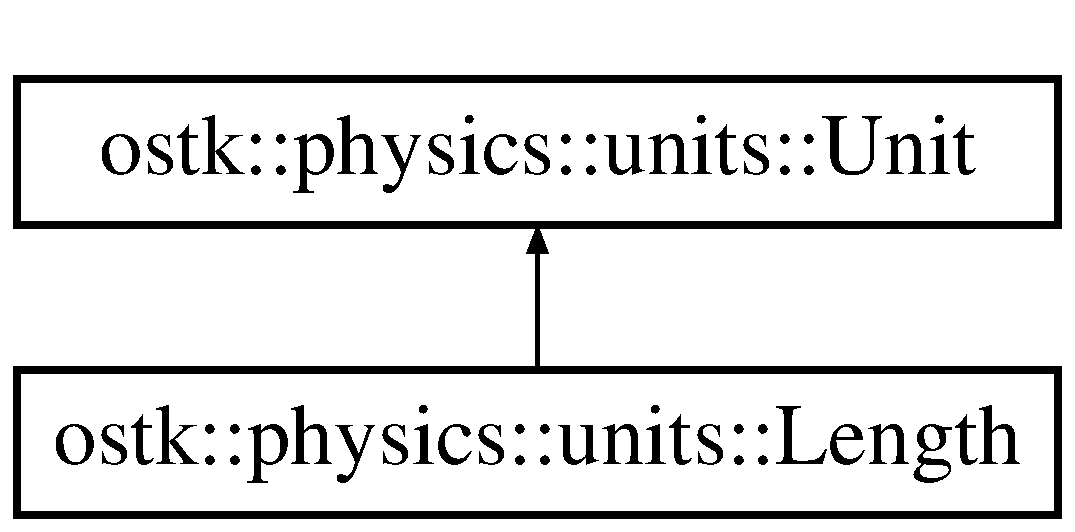
\includegraphics[height=2.000000cm]{classostk_1_1physics_1_1units_1_1_length}
\end{center}
\end{figure}
\subsection*{Public Types}
\begin{DoxyCompactItemize}
\item 
enum \hyperlink{classostk_1_1physics_1_1units_1_1_length_a2664470a7eedf5d45c88861fe69badea}{Unit} \{ \newline
\hyperlink{classostk_1_1physics_1_1units_1_1_length_a2664470a7eedf5d45c88861fe69badeaaec0fc0100c4fc1ce4eea230c3dc10360}{Unit\+::\+Undefined}, 
\hyperlink{classostk_1_1physics_1_1units_1_1_length_a2664470a7eedf5d45c88861fe69badeaa17c9c40b9db5a0983d1075a012c1f90a}{Unit\+::\+Meter}, 
\hyperlink{classostk_1_1physics_1_1units_1_1_length_a2664470a7eedf5d45c88861fe69badeaa129e74dde7b475c8848310e16754c965}{Unit\+::\+Foot}, 
\hyperlink{classostk_1_1physics_1_1units_1_1_length_a2664470a7eedf5d45c88861fe69badeaaf8e05509b5e8ce4f92f380304a29aa87}{Unit\+::\+Terrestrial\+Mile}, 
\newline
\hyperlink{classostk_1_1physics_1_1units_1_1_length_a2664470a7eedf5d45c88861fe69badeaa17728b6a29127fe1e34706ae1d691f42}{Unit\+::\+Nautical\+Mile}, 
\hyperlink{classostk_1_1physics_1_1units_1_1_length_a2664470a7eedf5d45c88861fe69badeaaa05a35804c7e4fff8e02f5a58782f133}{Unit\+::\+Astronomical\+Unit}
 \}
\end{DoxyCompactItemize}
\subsection*{Public Member Functions}
\begin{DoxyCompactItemize}
\item 
\hyperlink{classostk_1_1physics_1_1units_1_1_length_ae42146342ec60e8430fc111974c12366}{Length} (const Real \&a\+Value, const \hyperlink{classostk_1_1physics_1_1units_1_1_length_a2664470a7eedf5d45c88861fe69badea}{Length\+::\+Unit} \&a\+Unit)
\begin{DoxyCompactList}\small\item\em Constructor. \end{DoxyCompactList}\item 
virtual \hyperlink{classostk_1_1physics_1_1units_1_1_length}{Length} $\ast$ \hyperlink{classostk_1_1physics_1_1units_1_1_length_aeeb9cf27e0ea9bd818ad806cf3083658}{clone} () const override
\item 
bool \hyperlink{classostk_1_1physics_1_1units_1_1_length_ad3ee7b62d8dbfc4cbb626a5573092df0}{operator==} (const \hyperlink{classostk_1_1physics_1_1units_1_1_length}{Length} \&a\+Length) const
\item 
bool \hyperlink{classostk_1_1physics_1_1units_1_1_length_ab2f0fcca55d97a7d27d27b24ffba5e8c}{operator!=} (const \hyperlink{classostk_1_1physics_1_1units_1_1_length}{Length} \&a\+Length) const
\item 
bool \hyperlink{classostk_1_1physics_1_1units_1_1_length_aa90a1a4caa9d0343a2b6395a27f30417}{operator$<$} (const \hyperlink{classostk_1_1physics_1_1units_1_1_length}{Length} \&a\+Length) const
\item 
bool \hyperlink{classostk_1_1physics_1_1units_1_1_length_a065e01d99187bb5c6decf7b2a507a91c}{operator$<$=} (const \hyperlink{classostk_1_1physics_1_1units_1_1_length}{Length} \&a\+Length) const
\item 
bool \hyperlink{classostk_1_1physics_1_1units_1_1_length_a3a57f59386ae63906c8143c7dbfeb90e}{operator$>$} (const \hyperlink{classostk_1_1physics_1_1units_1_1_length}{Length} \&a\+Length) const
\item 
bool \hyperlink{classostk_1_1physics_1_1units_1_1_length_a365ab9cd6546cdbe76a05082a5ff88da}{operator$>$=} (const \hyperlink{classostk_1_1physics_1_1units_1_1_length}{Length} \&a\+Length) const
\item 
\hyperlink{classostk_1_1physics_1_1units_1_1_length}{Length} \hyperlink{classostk_1_1physics_1_1units_1_1_length_a75f9cc6530d47b20f5f0204f452b21ff}{operator+} (const \hyperlink{classostk_1_1physics_1_1units_1_1_length}{Length} \&a\+Length) const
\item 
\hyperlink{classostk_1_1physics_1_1units_1_1_length}{Length} \hyperlink{classostk_1_1physics_1_1units_1_1_length_a7ead71a73994b72fea9cbee1763c921f}{operator-\/} (const \hyperlink{classostk_1_1physics_1_1units_1_1_length}{Length} \&a\+Length) const
\item 
\hyperlink{classostk_1_1physics_1_1units_1_1_length}{Length} \hyperlink{classostk_1_1physics_1_1units_1_1_length_a58a2e430e8a6296e7eca6e5307d5805d}{operator$\ast$} (const Real \&a\+Real) const
\item 
\hyperlink{classostk_1_1physics_1_1units_1_1_length}{Length} \hyperlink{classostk_1_1physics_1_1units_1_1_length_a7fa05d1bb3642cb9bf8b46331f273e77}{operator/} (const Real \&a\+Real) const
\item 
\hyperlink{classostk_1_1physics_1_1units_1_1_length}{Length} \& \hyperlink{classostk_1_1physics_1_1units_1_1_length_a7903485eb0e4d3f92cdbd8436ecb5adc}{operator+=} (const \hyperlink{classostk_1_1physics_1_1units_1_1_length}{Length} \&a\+Length)
\item 
\hyperlink{classostk_1_1physics_1_1units_1_1_length}{Length} \& \hyperlink{classostk_1_1physics_1_1units_1_1_length_a9006163f65f5bb808a4956d5302f3802}{operator-\/=} (const \hyperlink{classostk_1_1physics_1_1units_1_1_length}{Length} \&a\+Length)
\item 
\hyperlink{classostk_1_1physics_1_1units_1_1_length}{Length} \& \hyperlink{classostk_1_1physics_1_1units_1_1_length_a6cb940402ce088d7b349bf4f4ca57cdf}{operator$\ast$=} (const Real \&a\+Real)
\item 
\hyperlink{classostk_1_1physics_1_1units_1_1_length}{Length} \& \hyperlink{classostk_1_1physics_1_1units_1_1_length_a5c174bd65d9f38fad8d84b82896d0ebb}{operator/=} (const Real \&a\+Real)
\item 
virtual bool \hyperlink{classostk_1_1physics_1_1units_1_1_length_aa176a675943dfe488fe96005c5405304}{is\+Defined} () const override
\item 
\hyperlink{classostk_1_1physics_1_1units_1_1_length_a2664470a7eedf5d45c88861fe69badea}{Length\+::\+Unit} \hyperlink{classostk_1_1physics_1_1units_1_1_length_a91a1b3cecc897c3f39519b26f01c431b}{get\+Unit} () const
\item 
Real \hyperlink{classostk_1_1physics_1_1units_1_1_length_ac4e43b2af197223ef81240b432f5b5af}{in} (const \hyperlink{classostk_1_1physics_1_1units_1_1_length_a2664470a7eedf5d45c88861fe69badea}{Length\+::\+Unit} \&a\+Unit) const
\item 
Real \hyperlink{classostk_1_1physics_1_1units_1_1_length_aa2d544dc47f218e40c13f498c00ae067}{in\+Meters} () const
\item 
Real \hyperlink{classostk_1_1physics_1_1units_1_1_length_a433a4673829f129b765b11ddce6c88b6}{in\+Kilometers} () const
\item 
virtual String \hyperlink{classostk_1_1physics_1_1units_1_1_length_ad3ec518939d2ffc86cd73b8ed4c071af}{to\+String} (const Integer \&a\+Precision=Integer\+::\+Undefined()) const override
\end{DoxyCompactItemize}
\subsection*{Static Public Member Functions}
\begin{DoxyCompactItemize}
\item 
static \hyperlink{classostk_1_1physics_1_1units_1_1_length}{Length} \hyperlink{classostk_1_1physics_1_1units_1_1_length_a1e76f961e57ed36274cf75e860b68726}{Undefined} ()
\item 
static \hyperlink{classostk_1_1physics_1_1units_1_1_length}{Length} \hyperlink{classostk_1_1physics_1_1units_1_1_length_a37a93f5c180723b39410c5e9757a9384}{Millimeters} (const Real \&a\+Value)
\item 
static \hyperlink{classostk_1_1physics_1_1units_1_1_length}{Length} \hyperlink{classostk_1_1physics_1_1units_1_1_length_ad227977ce00756791595796a0dd5ddd7}{Meters} (const Real \&a\+Value)
\item 
static \hyperlink{classostk_1_1physics_1_1units_1_1_length}{Length} \hyperlink{classostk_1_1physics_1_1units_1_1_length_accc55f3532825355cb54ab8e6bf970b9}{Kilometers} (const Real \&a\+Value)
\item 
static \hyperlink{classostk_1_1physics_1_1units_1_1_length}{Length} \hyperlink{classostk_1_1physics_1_1units_1_1_length_a757f89c932805e4bc75d691900ce406a}{Parse} (const String \&a\+String)
\item 
static String \hyperlink{classostk_1_1physics_1_1units_1_1_length_a0741ec3f518921e55ea97819bcd12f8e}{String\+From\+Unit} (const \hyperlink{classostk_1_1physics_1_1units_1_1_length_a2664470a7eedf5d45c88861fe69badea}{Length\+::\+Unit} \&a\+Unit)
\item 
static String \hyperlink{classostk_1_1physics_1_1units_1_1_length_a2747d33c0210375fd9c09ad75f90b822}{Symbol\+From\+Unit} (const \hyperlink{classostk_1_1physics_1_1units_1_1_length_a2664470a7eedf5d45c88861fe69badea}{Length\+::\+Unit} \&a\+Unit)
\item 
static \hyperlink{classostk_1_1physics_1_1units_1_1_length_a2664470a7eedf5d45c88861fe69badea}{Length\+::\+Unit} \hyperlink{classostk_1_1physics_1_1units_1_1_length_a91418e40747b13b0e2b669ec55626afa}{Unit\+From\+Symbol} (const String \&a\+Symbol)
\end{DoxyCompactItemize}
\subsection*{Friends}
\begin{DoxyCompactItemize}
\item 
\hyperlink{classostk_1_1physics_1_1units_1_1_length}{Length} \hyperlink{classostk_1_1physics_1_1units_1_1_length_a72059ec2f1e930a0e75a3a808e434363}{operator$\ast$} (const Real \&a\+Real, const \hyperlink{classostk_1_1physics_1_1units_1_1_length}{Length} \&a\+Length)
\item 
std\+::ostream \& \hyperlink{classostk_1_1physics_1_1units_1_1_length_a95a13170a8d57cb0060eae94520eace4}{operator$<$$<$} (std\+::ostream \&an\+Output\+Stream, const \hyperlink{classostk_1_1physics_1_1units_1_1_length}{Length} \&a\+Length)
\end{DoxyCompactItemize}
\subsection*{Additional Inherited Members}


\subsection{Detailed Description}
\hyperlink{classostk_1_1physics_1_1units_1_1_length}{Length}. 

https\+://en.wikipedia.\+org/wiki/\+Length 

\subsection{Member Enumeration Documentation}
\mbox{\Hypertarget{classostk_1_1physics_1_1units_1_1_length_a2664470a7eedf5d45c88861fe69badea}\label{classostk_1_1physics_1_1units_1_1_length_a2664470a7eedf5d45c88861fe69badea}} 
\index{ostk\+::physics\+::units\+::\+Length@{ostk\+::physics\+::units\+::\+Length}!Unit@{Unit}}
\index{Unit@{Unit}!ostk\+::physics\+::units\+::\+Length@{ostk\+::physics\+::units\+::\+Length}}
\subsubsection{\texorpdfstring{Unit}{Unit}}
{\footnotesize\ttfamily enum \hyperlink{classostk_1_1physics_1_1units_1_1_length_a2664470a7eedf5d45c88861fe69badea}{ostk\+::physics\+::units\+::\+Length\+::\+Unit}\hspace{0.3cm}{\ttfamily [strong]}}

\begin{DoxyEnumFields}{Enumerator}
\raisebox{\heightof{T}}[0pt][0pt]{\index{Undefined@{Undefined}!ostk\+::physics\+::units\+::\+Length@{ostk\+::physics\+::units\+::\+Length}}\index{ostk\+::physics\+::units\+::\+Length@{ostk\+::physics\+::units\+::\+Length}!Undefined@{Undefined}}}\mbox{\Hypertarget{classostk_1_1physics_1_1units_1_1_length_a2664470a7eedf5d45c88861fe69badeaaec0fc0100c4fc1ce4eea230c3dc10360}\label{classostk_1_1physics_1_1units_1_1_length_a2664470a7eedf5d45c88861fe69badeaaec0fc0100c4fc1ce4eea230c3dc10360}} 
Undefined&Undefined. \\
\hline

\raisebox{\heightof{T}}[0pt][0pt]{\index{Meter@{Meter}!ostk\+::physics\+::units\+::\+Length@{ostk\+::physics\+::units\+::\+Length}}\index{ostk\+::physics\+::units\+::\+Length@{ostk\+::physics\+::units\+::\+Length}!Meter@{Meter}}}\mbox{\Hypertarget{classostk_1_1physics_1_1units_1_1_length_a2664470a7eedf5d45c88861fe69badeaa17c9c40b9db5a0983d1075a012c1f90a}\label{classostk_1_1physics_1_1units_1_1_length_a2664470a7eedf5d45c88861fe69badeaa17c9c40b9db5a0983d1075a012c1f90a}} 
Meter&Meter (SI) \\
\hline

\raisebox{\heightof{T}}[0pt][0pt]{\index{Foot@{Foot}!ostk\+::physics\+::units\+::\+Length@{ostk\+::physics\+::units\+::\+Length}}\index{ostk\+::physics\+::units\+::\+Length@{ostk\+::physics\+::units\+::\+Length}!Foot@{Foot}}}\mbox{\Hypertarget{classostk_1_1physics_1_1units_1_1_length_a2664470a7eedf5d45c88861fe69badeaa129e74dde7b475c8848310e16754c965}\label{classostk_1_1physics_1_1units_1_1_length_a2664470a7eedf5d45c88861fe69badeaa129e74dde7b475c8848310e16754c965}} 
Foot&Foot. \\
\hline

\raisebox{\heightof{T}}[0pt][0pt]{\index{Terrestrial\+Mile@{Terrestrial\+Mile}!ostk\+::physics\+::units\+::\+Length@{ostk\+::physics\+::units\+::\+Length}}\index{ostk\+::physics\+::units\+::\+Length@{ostk\+::physics\+::units\+::\+Length}!Terrestrial\+Mile@{Terrestrial\+Mile}}}\mbox{\Hypertarget{classostk_1_1physics_1_1units_1_1_length_a2664470a7eedf5d45c88861fe69badeaaf8e05509b5e8ce4f92f380304a29aa87}\label{classostk_1_1physics_1_1units_1_1_length_a2664470a7eedf5d45c88861fe69badeaaf8e05509b5e8ce4f92f380304a29aa87}} 
Terrestrial\+Mile&Terrestrial mile. \\
\hline

\raisebox{\heightof{T}}[0pt][0pt]{\index{Nautical\+Mile@{Nautical\+Mile}!ostk\+::physics\+::units\+::\+Length@{ostk\+::physics\+::units\+::\+Length}}\index{ostk\+::physics\+::units\+::\+Length@{ostk\+::physics\+::units\+::\+Length}!Nautical\+Mile@{Nautical\+Mile}}}\mbox{\Hypertarget{classostk_1_1physics_1_1units_1_1_length_a2664470a7eedf5d45c88861fe69badeaa17728b6a29127fe1e34706ae1d691f42}\label{classostk_1_1physics_1_1units_1_1_length_a2664470a7eedf5d45c88861fe69badeaa17728b6a29127fe1e34706ae1d691f42}} 
Nautical\+Mile&Nautical mile. \\
\hline

\raisebox{\heightof{T}}[0pt][0pt]{\index{Astronomical\+Unit@{Astronomical\+Unit}!ostk\+::physics\+::units\+::\+Length@{ostk\+::physics\+::units\+::\+Length}}\index{ostk\+::physics\+::units\+::\+Length@{ostk\+::physics\+::units\+::\+Length}!Astronomical\+Unit@{Astronomical\+Unit}}}\mbox{\Hypertarget{classostk_1_1physics_1_1units_1_1_length_a2664470a7eedf5d45c88861fe69badeaaa05a35804c7e4fff8e02f5a58782f133}\label{classostk_1_1physics_1_1units_1_1_length_a2664470a7eedf5d45c88861fe69badeaaa05a35804c7e4fff8e02f5a58782f133}} 
Astronomical\+Unit&Astronomical \hyperlink{classostk_1_1physics_1_1units_1_1_unit}{Unit}. \\
\hline

\end{DoxyEnumFields}


\subsection{Constructor \& Destructor Documentation}
\mbox{\Hypertarget{classostk_1_1physics_1_1units_1_1_length_ae42146342ec60e8430fc111974c12366}\label{classostk_1_1physics_1_1units_1_1_length_ae42146342ec60e8430fc111974c12366}} 
\index{ostk\+::physics\+::units\+::\+Length@{ostk\+::physics\+::units\+::\+Length}!Length@{Length}}
\index{Length@{Length}!ostk\+::physics\+::units\+::\+Length@{ostk\+::physics\+::units\+::\+Length}}
\subsubsection{\texorpdfstring{Length()}{Length()}}
{\footnotesize\ttfamily ostk\+::physics\+::units\+::\+Length\+::\+Length (\begin{DoxyParamCaption}\item[{const Real \&}]{a\+Value,  }\item[{const \hyperlink{classostk_1_1physics_1_1units_1_1_length_a2664470a7eedf5d45c88861fe69badea}{Length\+::\+Unit} \&}]{a\+Unit }\end{DoxyParamCaption})}



Constructor. 


\begin{DoxyCode}
\hyperlink{classostk_1_1physics_1_1units_1_1_length_ae42146342ec60e8430fc111974c12366}{Length} length(1.0, \hyperlink{classostk_1_1physics_1_1units_1_1_length_a2664470a7eedf5d45c88861fe69badeaa17c9c40b9db5a0983d1075a012c1f90a}{Length::Unit::Meter}) ;
\end{DoxyCode}



\begin{DoxyParams}[1]{Parameters}
\mbox{\tt in}  & {\em a\+Value} & A value \\
\hline
\mbox{\tt in}  & {\em a\+Unit} & A length unit \\
\hline
\end{DoxyParams}


\subsection{Member Function Documentation}
\mbox{\Hypertarget{classostk_1_1physics_1_1units_1_1_length_aeeb9cf27e0ea9bd818ad806cf3083658}\label{classostk_1_1physics_1_1units_1_1_length_aeeb9cf27e0ea9bd818ad806cf3083658}} 
\index{ostk\+::physics\+::units\+::\+Length@{ostk\+::physics\+::units\+::\+Length}!clone@{clone}}
\index{clone@{clone}!ostk\+::physics\+::units\+::\+Length@{ostk\+::physics\+::units\+::\+Length}}
\subsubsection{\texorpdfstring{clone()}{clone()}}
{\footnotesize\ttfamily \hyperlink{classostk_1_1physics_1_1units_1_1_length}{Length} $\ast$ ostk\+::physics\+::units\+::\+Length\+::clone (\begin{DoxyParamCaption}{ }\end{DoxyParamCaption}) const\hspace{0.3cm}{\ttfamily [override]}, {\ttfamily [virtual]}}



Implements \hyperlink{classostk_1_1physics_1_1units_1_1_unit_ab203628f8a16b16c28d89eaa4c3aff67}{ostk\+::physics\+::units\+::\+Unit}.

\mbox{\Hypertarget{classostk_1_1physics_1_1units_1_1_length_a91a1b3cecc897c3f39519b26f01c431b}\label{classostk_1_1physics_1_1units_1_1_length_a91a1b3cecc897c3f39519b26f01c431b}} 
\index{ostk\+::physics\+::units\+::\+Length@{ostk\+::physics\+::units\+::\+Length}!get\+Unit@{get\+Unit}}
\index{get\+Unit@{get\+Unit}!ostk\+::physics\+::units\+::\+Length@{ostk\+::physics\+::units\+::\+Length}}
\subsubsection{\texorpdfstring{get\+Unit()}{getUnit()}}
{\footnotesize\ttfamily \hyperlink{classostk_1_1physics_1_1units_1_1_length_a2664470a7eedf5d45c88861fe69badea}{Length\+::\+Unit} ostk\+::physics\+::units\+::\+Length\+::get\+Unit (\begin{DoxyParamCaption}{ }\end{DoxyParamCaption}) const}

\mbox{\Hypertarget{classostk_1_1physics_1_1units_1_1_length_ac4e43b2af197223ef81240b432f5b5af}\label{classostk_1_1physics_1_1units_1_1_length_ac4e43b2af197223ef81240b432f5b5af}} 
\index{ostk\+::physics\+::units\+::\+Length@{ostk\+::physics\+::units\+::\+Length}!in@{in}}
\index{in@{in}!ostk\+::physics\+::units\+::\+Length@{ostk\+::physics\+::units\+::\+Length}}
\subsubsection{\texorpdfstring{in()}{in()}}
{\footnotesize\ttfamily Real ostk\+::physics\+::units\+::\+Length\+::in (\begin{DoxyParamCaption}\item[{const \hyperlink{classostk_1_1physics_1_1units_1_1_length_a2664470a7eedf5d45c88861fe69badea}{Length\+::\+Unit} \&}]{a\+Unit }\end{DoxyParamCaption}) const}

\mbox{\Hypertarget{classostk_1_1physics_1_1units_1_1_length_a433a4673829f129b765b11ddce6c88b6}\label{classostk_1_1physics_1_1units_1_1_length_a433a4673829f129b765b11ddce6c88b6}} 
\index{ostk\+::physics\+::units\+::\+Length@{ostk\+::physics\+::units\+::\+Length}!in\+Kilometers@{in\+Kilometers}}
\index{in\+Kilometers@{in\+Kilometers}!ostk\+::physics\+::units\+::\+Length@{ostk\+::physics\+::units\+::\+Length}}
\subsubsection{\texorpdfstring{in\+Kilometers()}{inKilometers()}}
{\footnotesize\ttfamily Real ostk\+::physics\+::units\+::\+Length\+::in\+Kilometers (\begin{DoxyParamCaption}{ }\end{DoxyParamCaption}) const}

\mbox{\Hypertarget{classostk_1_1physics_1_1units_1_1_length_aa2d544dc47f218e40c13f498c00ae067}\label{classostk_1_1physics_1_1units_1_1_length_aa2d544dc47f218e40c13f498c00ae067}} 
\index{ostk\+::physics\+::units\+::\+Length@{ostk\+::physics\+::units\+::\+Length}!in\+Meters@{in\+Meters}}
\index{in\+Meters@{in\+Meters}!ostk\+::physics\+::units\+::\+Length@{ostk\+::physics\+::units\+::\+Length}}
\subsubsection{\texorpdfstring{in\+Meters()}{inMeters()}}
{\footnotesize\ttfamily Real ostk\+::physics\+::units\+::\+Length\+::in\+Meters (\begin{DoxyParamCaption}{ }\end{DoxyParamCaption}) const}

\mbox{\Hypertarget{classostk_1_1physics_1_1units_1_1_length_aa176a675943dfe488fe96005c5405304}\label{classostk_1_1physics_1_1units_1_1_length_aa176a675943dfe488fe96005c5405304}} 
\index{ostk\+::physics\+::units\+::\+Length@{ostk\+::physics\+::units\+::\+Length}!is\+Defined@{is\+Defined}}
\index{is\+Defined@{is\+Defined}!ostk\+::physics\+::units\+::\+Length@{ostk\+::physics\+::units\+::\+Length}}
\subsubsection{\texorpdfstring{is\+Defined()}{isDefined()}}
{\footnotesize\ttfamily bool ostk\+::physics\+::units\+::\+Length\+::is\+Defined (\begin{DoxyParamCaption}{ }\end{DoxyParamCaption}) const\hspace{0.3cm}{\ttfamily [override]}, {\ttfamily [virtual]}}



Reimplemented from \hyperlink{classostk_1_1physics_1_1units_1_1_unit_a423ce1df3478f0892b10824b591ae1cc}{ostk\+::physics\+::units\+::\+Unit}.

\mbox{\Hypertarget{classostk_1_1physics_1_1units_1_1_length_accc55f3532825355cb54ab8e6bf970b9}\label{classostk_1_1physics_1_1units_1_1_length_accc55f3532825355cb54ab8e6bf970b9}} 
\index{ostk\+::physics\+::units\+::\+Length@{ostk\+::physics\+::units\+::\+Length}!Kilometers@{Kilometers}}
\index{Kilometers@{Kilometers}!ostk\+::physics\+::units\+::\+Length@{ostk\+::physics\+::units\+::\+Length}}
\subsubsection{\texorpdfstring{Kilometers()}{Kilometers()}}
{\footnotesize\ttfamily \hyperlink{classostk_1_1physics_1_1units_1_1_length}{Length} ostk\+::physics\+::units\+::\+Length\+::\+Kilometers (\begin{DoxyParamCaption}\item[{const Real \&}]{a\+Value }\end{DoxyParamCaption})\hspace{0.3cm}{\ttfamily [static]}}

\mbox{\Hypertarget{classostk_1_1physics_1_1units_1_1_length_ad227977ce00756791595796a0dd5ddd7}\label{classostk_1_1physics_1_1units_1_1_length_ad227977ce00756791595796a0dd5ddd7}} 
\index{ostk\+::physics\+::units\+::\+Length@{ostk\+::physics\+::units\+::\+Length}!Meters@{Meters}}
\index{Meters@{Meters}!ostk\+::physics\+::units\+::\+Length@{ostk\+::physics\+::units\+::\+Length}}
\subsubsection{\texorpdfstring{Meters()}{Meters()}}
{\footnotesize\ttfamily \hyperlink{classostk_1_1physics_1_1units_1_1_length}{Length} ostk\+::physics\+::units\+::\+Length\+::\+Meters (\begin{DoxyParamCaption}\item[{const Real \&}]{a\+Value }\end{DoxyParamCaption})\hspace{0.3cm}{\ttfamily [static]}}

\mbox{\Hypertarget{classostk_1_1physics_1_1units_1_1_length_a37a93f5c180723b39410c5e9757a9384}\label{classostk_1_1physics_1_1units_1_1_length_a37a93f5c180723b39410c5e9757a9384}} 
\index{ostk\+::physics\+::units\+::\+Length@{ostk\+::physics\+::units\+::\+Length}!Millimeters@{Millimeters}}
\index{Millimeters@{Millimeters}!ostk\+::physics\+::units\+::\+Length@{ostk\+::physics\+::units\+::\+Length}}
\subsubsection{\texorpdfstring{Millimeters()}{Millimeters()}}
{\footnotesize\ttfamily \hyperlink{classostk_1_1physics_1_1units_1_1_length}{Length} ostk\+::physics\+::units\+::\+Length\+::\+Millimeters (\begin{DoxyParamCaption}\item[{const Real \&}]{a\+Value }\end{DoxyParamCaption})\hspace{0.3cm}{\ttfamily [static]}}

\mbox{\Hypertarget{classostk_1_1physics_1_1units_1_1_length_ab2f0fcca55d97a7d27d27b24ffba5e8c}\label{classostk_1_1physics_1_1units_1_1_length_ab2f0fcca55d97a7d27d27b24ffba5e8c}} 
\index{ostk\+::physics\+::units\+::\+Length@{ostk\+::physics\+::units\+::\+Length}!operator"!=@{operator"!=}}
\index{operator"!=@{operator"!=}!ostk\+::physics\+::units\+::\+Length@{ostk\+::physics\+::units\+::\+Length}}
\subsubsection{\texorpdfstring{operator"!=()}{operator!=()}}
{\footnotesize\ttfamily bool ostk\+::physics\+::units\+::\+Length\+::operator!= (\begin{DoxyParamCaption}\item[{const \hyperlink{classostk_1_1physics_1_1units_1_1_length}{Length} \&}]{a\+Length }\end{DoxyParamCaption}) const}

\mbox{\Hypertarget{classostk_1_1physics_1_1units_1_1_length_a58a2e430e8a6296e7eca6e5307d5805d}\label{classostk_1_1physics_1_1units_1_1_length_a58a2e430e8a6296e7eca6e5307d5805d}} 
\index{ostk\+::physics\+::units\+::\+Length@{ostk\+::physics\+::units\+::\+Length}!operator$\ast$@{operator$\ast$}}
\index{operator$\ast$@{operator$\ast$}!ostk\+::physics\+::units\+::\+Length@{ostk\+::physics\+::units\+::\+Length}}
\subsubsection{\texorpdfstring{operator$\ast$()}{operator*()}}
{\footnotesize\ttfamily \hyperlink{classostk_1_1physics_1_1units_1_1_length}{Length} ostk\+::physics\+::units\+::\+Length\+::operator$\ast$ (\begin{DoxyParamCaption}\item[{const Real \&}]{a\+Real }\end{DoxyParamCaption}) const}

\mbox{\Hypertarget{classostk_1_1physics_1_1units_1_1_length_a6cb940402ce088d7b349bf4f4ca57cdf}\label{classostk_1_1physics_1_1units_1_1_length_a6cb940402ce088d7b349bf4f4ca57cdf}} 
\index{ostk\+::physics\+::units\+::\+Length@{ostk\+::physics\+::units\+::\+Length}!operator$\ast$=@{operator$\ast$=}}
\index{operator$\ast$=@{operator$\ast$=}!ostk\+::physics\+::units\+::\+Length@{ostk\+::physics\+::units\+::\+Length}}
\subsubsection{\texorpdfstring{operator$\ast$=()}{operator*=()}}
{\footnotesize\ttfamily \hyperlink{classostk_1_1physics_1_1units_1_1_length}{Length} \& ostk\+::physics\+::units\+::\+Length\+::operator$\ast$= (\begin{DoxyParamCaption}\item[{const Real \&}]{a\+Real }\end{DoxyParamCaption})}

\mbox{\Hypertarget{classostk_1_1physics_1_1units_1_1_length_a75f9cc6530d47b20f5f0204f452b21ff}\label{classostk_1_1physics_1_1units_1_1_length_a75f9cc6530d47b20f5f0204f452b21ff}} 
\index{ostk\+::physics\+::units\+::\+Length@{ostk\+::physics\+::units\+::\+Length}!operator+@{operator+}}
\index{operator+@{operator+}!ostk\+::physics\+::units\+::\+Length@{ostk\+::physics\+::units\+::\+Length}}
\subsubsection{\texorpdfstring{operator+()}{operator+()}}
{\footnotesize\ttfamily \hyperlink{classostk_1_1physics_1_1units_1_1_length}{Length} ostk\+::physics\+::units\+::\+Length\+::operator+ (\begin{DoxyParamCaption}\item[{const \hyperlink{classostk_1_1physics_1_1units_1_1_length}{Length} \&}]{a\+Length }\end{DoxyParamCaption}) const}

\mbox{\Hypertarget{classostk_1_1physics_1_1units_1_1_length_a7903485eb0e4d3f92cdbd8436ecb5adc}\label{classostk_1_1physics_1_1units_1_1_length_a7903485eb0e4d3f92cdbd8436ecb5adc}} 
\index{ostk\+::physics\+::units\+::\+Length@{ostk\+::physics\+::units\+::\+Length}!operator+=@{operator+=}}
\index{operator+=@{operator+=}!ostk\+::physics\+::units\+::\+Length@{ostk\+::physics\+::units\+::\+Length}}
\subsubsection{\texorpdfstring{operator+=()}{operator+=()}}
{\footnotesize\ttfamily \hyperlink{classostk_1_1physics_1_1units_1_1_length}{Length} \& ostk\+::physics\+::units\+::\+Length\+::operator+= (\begin{DoxyParamCaption}\item[{const \hyperlink{classostk_1_1physics_1_1units_1_1_length}{Length} \&}]{a\+Length }\end{DoxyParamCaption})}

\mbox{\Hypertarget{classostk_1_1physics_1_1units_1_1_length_a7ead71a73994b72fea9cbee1763c921f}\label{classostk_1_1physics_1_1units_1_1_length_a7ead71a73994b72fea9cbee1763c921f}} 
\index{ostk\+::physics\+::units\+::\+Length@{ostk\+::physics\+::units\+::\+Length}!operator-\/@{operator-\/}}
\index{operator-\/@{operator-\/}!ostk\+::physics\+::units\+::\+Length@{ostk\+::physics\+::units\+::\+Length}}
\subsubsection{\texorpdfstring{operator-\/()}{operator-()}}
{\footnotesize\ttfamily \hyperlink{classostk_1_1physics_1_1units_1_1_length}{Length} ostk\+::physics\+::units\+::\+Length\+::operator-\/ (\begin{DoxyParamCaption}\item[{const \hyperlink{classostk_1_1physics_1_1units_1_1_length}{Length} \&}]{a\+Length }\end{DoxyParamCaption}) const}

\mbox{\Hypertarget{classostk_1_1physics_1_1units_1_1_length_a9006163f65f5bb808a4956d5302f3802}\label{classostk_1_1physics_1_1units_1_1_length_a9006163f65f5bb808a4956d5302f3802}} 
\index{ostk\+::physics\+::units\+::\+Length@{ostk\+::physics\+::units\+::\+Length}!operator-\/=@{operator-\/=}}
\index{operator-\/=@{operator-\/=}!ostk\+::physics\+::units\+::\+Length@{ostk\+::physics\+::units\+::\+Length}}
\subsubsection{\texorpdfstring{operator-\/=()}{operator-=()}}
{\footnotesize\ttfamily \hyperlink{classostk_1_1physics_1_1units_1_1_length}{Length} \& ostk\+::physics\+::units\+::\+Length\+::operator-\/= (\begin{DoxyParamCaption}\item[{const \hyperlink{classostk_1_1physics_1_1units_1_1_length}{Length} \&}]{a\+Length }\end{DoxyParamCaption})}

\mbox{\Hypertarget{classostk_1_1physics_1_1units_1_1_length_a7fa05d1bb3642cb9bf8b46331f273e77}\label{classostk_1_1physics_1_1units_1_1_length_a7fa05d1bb3642cb9bf8b46331f273e77}} 
\index{ostk\+::physics\+::units\+::\+Length@{ostk\+::physics\+::units\+::\+Length}!operator/@{operator/}}
\index{operator/@{operator/}!ostk\+::physics\+::units\+::\+Length@{ostk\+::physics\+::units\+::\+Length}}
\subsubsection{\texorpdfstring{operator/()}{operator/()}}
{\footnotesize\ttfamily \hyperlink{classostk_1_1physics_1_1units_1_1_length}{Length} ostk\+::physics\+::units\+::\+Length\+::operator/ (\begin{DoxyParamCaption}\item[{const Real \&}]{a\+Real }\end{DoxyParamCaption}) const}

\mbox{\Hypertarget{classostk_1_1physics_1_1units_1_1_length_a5c174bd65d9f38fad8d84b82896d0ebb}\label{classostk_1_1physics_1_1units_1_1_length_a5c174bd65d9f38fad8d84b82896d0ebb}} 
\index{ostk\+::physics\+::units\+::\+Length@{ostk\+::physics\+::units\+::\+Length}!operator/=@{operator/=}}
\index{operator/=@{operator/=}!ostk\+::physics\+::units\+::\+Length@{ostk\+::physics\+::units\+::\+Length}}
\subsubsection{\texorpdfstring{operator/=()}{operator/=()}}
{\footnotesize\ttfamily \hyperlink{classostk_1_1physics_1_1units_1_1_length}{Length} \& ostk\+::physics\+::units\+::\+Length\+::operator/= (\begin{DoxyParamCaption}\item[{const Real \&}]{a\+Real }\end{DoxyParamCaption})}

\mbox{\Hypertarget{classostk_1_1physics_1_1units_1_1_length_aa90a1a4caa9d0343a2b6395a27f30417}\label{classostk_1_1physics_1_1units_1_1_length_aa90a1a4caa9d0343a2b6395a27f30417}} 
\index{ostk\+::physics\+::units\+::\+Length@{ostk\+::physics\+::units\+::\+Length}!operator$<$@{operator$<$}}
\index{operator$<$@{operator$<$}!ostk\+::physics\+::units\+::\+Length@{ostk\+::physics\+::units\+::\+Length}}
\subsubsection{\texorpdfstring{operator$<$()}{operator<()}}
{\footnotesize\ttfamily bool ostk\+::physics\+::units\+::\+Length\+::operator$<$ (\begin{DoxyParamCaption}\item[{const \hyperlink{classostk_1_1physics_1_1units_1_1_length}{Length} \&}]{a\+Length }\end{DoxyParamCaption}) const}

\mbox{\Hypertarget{classostk_1_1physics_1_1units_1_1_length_a065e01d99187bb5c6decf7b2a507a91c}\label{classostk_1_1physics_1_1units_1_1_length_a065e01d99187bb5c6decf7b2a507a91c}} 
\index{ostk\+::physics\+::units\+::\+Length@{ostk\+::physics\+::units\+::\+Length}!operator$<$=@{operator$<$=}}
\index{operator$<$=@{operator$<$=}!ostk\+::physics\+::units\+::\+Length@{ostk\+::physics\+::units\+::\+Length}}
\subsubsection{\texorpdfstring{operator$<$=()}{operator<=()}}
{\footnotesize\ttfamily bool ostk\+::physics\+::units\+::\+Length\+::operator$<$= (\begin{DoxyParamCaption}\item[{const \hyperlink{classostk_1_1physics_1_1units_1_1_length}{Length} \&}]{a\+Length }\end{DoxyParamCaption}) const}

\mbox{\Hypertarget{classostk_1_1physics_1_1units_1_1_length_ad3ee7b62d8dbfc4cbb626a5573092df0}\label{classostk_1_1physics_1_1units_1_1_length_ad3ee7b62d8dbfc4cbb626a5573092df0}} 
\index{ostk\+::physics\+::units\+::\+Length@{ostk\+::physics\+::units\+::\+Length}!operator==@{operator==}}
\index{operator==@{operator==}!ostk\+::physics\+::units\+::\+Length@{ostk\+::physics\+::units\+::\+Length}}
\subsubsection{\texorpdfstring{operator==()}{operator==()}}
{\footnotesize\ttfamily bool ostk\+::physics\+::units\+::\+Length\+::operator== (\begin{DoxyParamCaption}\item[{const \hyperlink{classostk_1_1physics_1_1units_1_1_length}{Length} \&}]{a\+Length }\end{DoxyParamCaption}) const}

\mbox{\Hypertarget{classostk_1_1physics_1_1units_1_1_length_a3a57f59386ae63906c8143c7dbfeb90e}\label{classostk_1_1physics_1_1units_1_1_length_a3a57f59386ae63906c8143c7dbfeb90e}} 
\index{ostk\+::physics\+::units\+::\+Length@{ostk\+::physics\+::units\+::\+Length}!operator$>$@{operator$>$}}
\index{operator$>$@{operator$>$}!ostk\+::physics\+::units\+::\+Length@{ostk\+::physics\+::units\+::\+Length}}
\subsubsection{\texorpdfstring{operator$>$()}{operator>()}}
{\footnotesize\ttfamily bool ostk\+::physics\+::units\+::\+Length\+::operator$>$ (\begin{DoxyParamCaption}\item[{const \hyperlink{classostk_1_1physics_1_1units_1_1_length}{Length} \&}]{a\+Length }\end{DoxyParamCaption}) const}

\mbox{\Hypertarget{classostk_1_1physics_1_1units_1_1_length_a365ab9cd6546cdbe76a05082a5ff88da}\label{classostk_1_1physics_1_1units_1_1_length_a365ab9cd6546cdbe76a05082a5ff88da}} 
\index{ostk\+::physics\+::units\+::\+Length@{ostk\+::physics\+::units\+::\+Length}!operator$>$=@{operator$>$=}}
\index{operator$>$=@{operator$>$=}!ostk\+::physics\+::units\+::\+Length@{ostk\+::physics\+::units\+::\+Length}}
\subsubsection{\texorpdfstring{operator$>$=()}{operator>=()}}
{\footnotesize\ttfamily bool ostk\+::physics\+::units\+::\+Length\+::operator$>$= (\begin{DoxyParamCaption}\item[{const \hyperlink{classostk_1_1physics_1_1units_1_1_length}{Length} \&}]{a\+Length }\end{DoxyParamCaption}) const}

\mbox{\Hypertarget{classostk_1_1physics_1_1units_1_1_length_a757f89c932805e4bc75d691900ce406a}\label{classostk_1_1physics_1_1units_1_1_length_a757f89c932805e4bc75d691900ce406a}} 
\index{ostk\+::physics\+::units\+::\+Length@{ostk\+::physics\+::units\+::\+Length}!Parse@{Parse}}
\index{Parse@{Parse}!ostk\+::physics\+::units\+::\+Length@{ostk\+::physics\+::units\+::\+Length}}
\subsubsection{\texorpdfstring{Parse()}{Parse()}}
{\footnotesize\ttfamily \hyperlink{classostk_1_1physics_1_1units_1_1_length}{Length} ostk\+::physics\+::units\+::\+Length\+::\+Parse (\begin{DoxyParamCaption}\item[{const String \&}]{a\+String }\end{DoxyParamCaption})\hspace{0.3cm}{\ttfamily [static]}}

\mbox{\Hypertarget{classostk_1_1physics_1_1units_1_1_length_a0741ec3f518921e55ea97819bcd12f8e}\label{classostk_1_1physics_1_1units_1_1_length_a0741ec3f518921e55ea97819bcd12f8e}} 
\index{ostk\+::physics\+::units\+::\+Length@{ostk\+::physics\+::units\+::\+Length}!String\+From\+Unit@{String\+From\+Unit}}
\index{String\+From\+Unit@{String\+From\+Unit}!ostk\+::physics\+::units\+::\+Length@{ostk\+::physics\+::units\+::\+Length}}
\subsubsection{\texorpdfstring{String\+From\+Unit()}{StringFromUnit()}}
{\footnotesize\ttfamily String ostk\+::physics\+::units\+::\+Length\+::\+String\+From\+Unit (\begin{DoxyParamCaption}\item[{const \hyperlink{classostk_1_1physics_1_1units_1_1_length_a2664470a7eedf5d45c88861fe69badea}{Length\+::\+Unit} \&}]{a\+Unit }\end{DoxyParamCaption})\hspace{0.3cm}{\ttfamily [static]}}

\mbox{\Hypertarget{classostk_1_1physics_1_1units_1_1_length_a2747d33c0210375fd9c09ad75f90b822}\label{classostk_1_1physics_1_1units_1_1_length_a2747d33c0210375fd9c09ad75f90b822}} 
\index{ostk\+::physics\+::units\+::\+Length@{ostk\+::physics\+::units\+::\+Length}!Symbol\+From\+Unit@{Symbol\+From\+Unit}}
\index{Symbol\+From\+Unit@{Symbol\+From\+Unit}!ostk\+::physics\+::units\+::\+Length@{ostk\+::physics\+::units\+::\+Length}}
\subsubsection{\texorpdfstring{Symbol\+From\+Unit()}{SymbolFromUnit()}}
{\footnotesize\ttfamily String ostk\+::physics\+::units\+::\+Length\+::\+Symbol\+From\+Unit (\begin{DoxyParamCaption}\item[{const \hyperlink{classostk_1_1physics_1_1units_1_1_length_a2664470a7eedf5d45c88861fe69badea}{Length\+::\+Unit} \&}]{a\+Unit }\end{DoxyParamCaption})\hspace{0.3cm}{\ttfamily [static]}}

\mbox{\Hypertarget{classostk_1_1physics_1_1units_1_1_length_ad3ec518939d2ffc86cd73b8ed4c071af}\label{classostk_1_1physics_1_1units_1_1_length_ad3ec518939d2ffc86cd73b8ed4c071af}} 
\index{ostk\+::physics\+::units\+::\+Length@{ostk\+::physics\+::units\+::\+Length}!to\+String@{to\+String}}
\index{to\+String@{to\+String}!ostk\+::physics\+::units\+::\+Length@{ostk\+::physics\+::units\+::\+Length}}
\subsubsection{\texorpdfstring{to\+String()}{toString()}}
{\footnotesize\ttfamily String ostk\+::physics\+::units\+::\+Length\+::to\+String (\begin{DoxyParamCaption}\item[{const Integer \&}]{a\+Precision = {\ttfamily Integer\+:\+:Undefined()} }\end{DoxyParamCaption}) const\hspace{0.3cm}{\ttfamily [override]}, {\ttfamily [virtual]}}



Implements \hyperlink{classostk_1_1physics_1_1units_1_1_unit_a8162b4eb8221c7577af16ab8b399d07e}{ostk\+::physics\+::units\+::\+Unit}.

\mbox{\Hypertarget{classostk_1_1physics_1_1units_1_1_length_a1e76f961e57ed36274cf75e860b68726}\label{classostk_1_1physics_1_1units_1_1_length_a1e76f961e57ed36274cf75e860b68726}} 
\index{ostk\+::physics\+::units\+::\+Length@{ostk\+::physics\+::units\+::\+Length}!Undefined@{Undefined}}
\index{Undefined@{Undefined}!ostk\+::physics\+::units\+::\+Length@{ostk\+::physics\+::units\+::\+Length}}
\subsubsection{\texorpdfstring{Undefined()}{Undefined()}}
{\footnotesize\ttfamily \hyperlink{classostk_1_1physics_1_1units_1_1_length}{Length} ostk\+::physics\+::units\+::\+Length\+::\+Undefined (\begin{DoxyParamCaption}{ }\end{DoxyParamCaption})\hspace{0.3cm}{\ttfamily [static]}}

\mbox{\Hypertarget{classostk_1_1physics_1_1units_1_1_length_a91418e40747b13b0e2b669ec55626afa}\label{classostk_1_1physics_1_1units_1_1_length_a91418e40747b13b0e2b669ec55626afa}} 
\index{ostk\+::physics\+::units\+::\+Length@{ostk\+::physics\+::units\+::\+Length}!Unit\+From\+Symbol@{Unit\+From\+Symbol}}
\index{Unit\+From\+Symbol@{Unit\+From\+Symbol}!ostk\+::physics\+::units\+::\+Length@{ostk\+::physics\+::units\+::\+Length}}
\subsubsection{\texorpdfstring{Unit\+From\+Symbol()}{UnitFromSymbol()}}
{\footnotesize\ttfamily \hyperlink{classostk_1_1physics_1_1units_1_1_length_a2664470a7eedf5d45c88861fe69badea}{Length\+::\+Unit} ostk\+::physics\+::units\+::\+Length\+::\+Unit\+From\+Symbol (\begin{DoxyParamCaption}\item[{const String \&}]{a\+Symbol }\end{DoxyParamCaption})\hspace{0.3cm}{\ttfamily [static]}}



\subsection{Friends And Related Function Documentation}
\mbox{\Hypertarget{classostk_1_1physics_1_1units_1_1_length_a72059ec2f1e930a0e75a3a808e434363}\label{classostk_1_1physics_1_1units_1_1_length_a72059ec2f1e930a0e75a3a808e434363}} 
\index{ostk\+::physics\+::units\+::\+Length@{ostk\+::physics\+::units\+::\+Length}!operator$\ast$@{operator$\ast$}}
\index{operator$\ast$@{operator$\ast$}!ostk\+::physics\+::units\+::\+Length@{ostk\+::physics\+::units\+::\+Length}}
\subsubsection{\texorpdfstring{operator$\ast$}{operator*}}
{\footnotesize\ttfamily \hyperlink{classostk_1_1physics_1_1units_1_1_length}{Length} operator$\ast$ (\begin{DoxyParamCaption}\item[{const Real \&}]{a\+Real,  }\item[{const \hyperlink{classostk_1_1physics_1_1units_1_1_length}{Length} \&}]{a\+Length }\end{DoxyParamCaption})\hspace{0.3cm}{\ttfamily [friend]}}

\mbox{\Hypertarget{classostk_1_1physics_1_1units_1_1_length_a95a13170a8d57cb0060eae94520eace4}\label{classostk_1_1physics_1_1units_1_1_length_a95a13170a8d57cb0060eae94520eace4}} 
\index{ostk\+::physics\+::units\+::\+Length@{ostk\+::physics\+::units\+::\+Length}!operator$<$$<$@{operator$<$$<$}}
\index{operator$<$$<$@{operator$<$$<$}!ostk\+::physics\+::units\+::\+Length@{ostk\+::physics\+::units\+::\+Length}}
\subsubsection{\texorpdfstring{operator$<$$<$}{operator<<}}
{\footnotesize\ttfamily std\+::ostream\& operator$<$$<$ (\begin{DoxyParamCaption}\item[{std\+::ostream \&}]{an\+Output\+Stream,  }\item[{const \hyperlink{classostk_1_1physics_1_1units_1_1_length}{Length} \&}]{a\+Length }\end{DoxyParamCaption})\hspace{0.3cm}{\ttfamily [friend]}}



The documentation for this class was generated from the following files\+:\begin{DoxyCompactItemize}
\item 
include/\+Open\+Space\+Toolkit/\+Physics/\+Units/\hyperlink{_length_8hpp}{Length.\+hpp}\item 
src/\+Open\+Space\+Toolkit/\+Physics/\+Units/\hyperlink{_length_8cpp}{Length.\+cpp}\end{DoxyCompactItemize}

\hypertarget{classostk_1_1physics_1_1coord_1_1spherical_1_1_l_l_a}{}\section{ostk\+:\+:physics\+:\+:coord\+:\+:spherical\+:\+:L\+LA Class Reference}
\label{classostk_1_1physics_1_1coord_1_1spherical_1_1_l_l_a}\index{ostk\+::physics\+::coord\+::spherical\+::\+L\+LA@{ostk\+::physics\+::coord\+::spherical\+::\+L\+LA}}


Geodetic Latitude -\/ Longitude -\/ Altitude (\hyperlink{classostk_1_1physics_1_1coord_1_1spherical_1_1_l_l_a}{L\+LA})  




{\ttfamily \#include $<$L\+L\+A.\+hpp$>$}

\subsection*{Public Member Functions}
\begin{DoxyCompactItemize}
\item 
\hyperlink{classostk_1_1physics_1_1coord_1_1spherical_1_1_l_l_a_a5a168b8087f0cfabca76b82870f6324a}{L\+LA} (const \hyperlink{classostk_1_1physics_1_1units_1_1_angle}{Angle} \&a\+Latitude, const \hyperlink{classostk_1_1physics_1_1units_1_1_angle}{Angle} \&a\+Longitude, const \hyperlink{classostk_1_1physics_1_1units_1_1_length}{Length} \&an\+Altitude)
\item 
bool \hyperlink{classostk_1_1physics_1_1coord_1_1spherical_1_1_l_l_a_addc7b917791049b8311821e56f5d29c9}{operator==} (const \hyperlink{classostk_1_1physics_1_1coord_1_1spherical_1_1_l_l_a}{L\+LA} \&a\+L\+LA) const
\item 
bool \hyperlink{classostk_1_1physics_1_1coord_1_1spherical_1_1_l_l_a_ae2568ab8a2969e0b5ecdb17592c71d53}{operator!=} (const \hyperlink{classostk_1_1physics_1_1coord_1_1spherical_1_1_l_l_a}{L\+LA} \&a\+L\+LA) const
\item 
bool \hyperlink{classostk_1_1physics_1_1coord_1_1spherical_1_1_l_l_a_a97649adf97bafbb9aa8cce36b30f920e}{is\+Defined} () const
\item 
\hyperlink{classostk_1_1physics_1_1units_1_1_angle}{Angle} \hyperlink{classostk_1_1physics_1_1coord_1_1spherical_1_1_l_l_a_a0b6d5f7409e1efbff0f01a9c00a876e8}{get\+Latitude} () const
\item 
\hyperlink{classostk_1_1physics_1_1units_1_1_angle}{Angle} \hyperlink{classostk_1_1physics_1_1coord_1_1spherical_1_1_l_l_a_aa031e4c4f1078cec374f0d4b0cc6e20d}{get\+Longitude} () const
\item 
\hyperlink{classostk_1_1physics_1_1units_1_1_length}{Length} \hyperlink{classostk_1_1physics_1_1coord_1_1spherical_1_1_l_l_a_a69214fc582c7d81ed8ddfbb28e7392a1}{get\+Altitude} () const
\item 
Vector3d \hyperlink{classostk_1_1physics_1_1coord_1_1spherical_1_1_l_l_a_add96410a645a57ddbe8d0d57c38885e0}{to\+Vector} () const
\item 
Vector3d \hyperlink{classostk_1_1physics_1_1coord_1_1spherical_1_1_l_l_a_a0bd2de41b2e1363414eb5bdc889d6a8e}{to\+Cartesian} (const \hyperlink{classostk_1_1physics_1_1units_1_1_length}{Length} \&an\+Ellipsoid\+Equatorial\+Radius, const Real \&an\+Ellipsoid\+Flattening) const
\item 
String \hyperlink{classostk_1_1physics_1_1coord_1_1spherical_1_1_l_l_a_adbab483b5d5a63fc507da0cd51db62ae}{to\+String} () const
\end{DoxyCompactItemize}
\subsection*{Static Public Member Functions}
\begin{DoxyCompactItemize}
\item 
static \hyperlink{classostk_1_1physics_1_1coord_1_1spherical_1_1_l_l_a}{L\+LA} \hyperlink{classostk_1_1physics_1_1coord_1_1spherical_1_1_l_l_a_ac02d0b9cb58f21d188ea025521f17c65}{Undefined} ()
\item 
static \hyperlink{classostk_1_1physics_1_1coord_1_1spherical_1_1_l_l_a}{L\+LA} \hyperlink{classostk_1_1physics_1_1coord_1_1spherical_1_1_l_l_a_a4a62e2c9995057dc14d1606e6be65fb8}{Vector} (const Vector3d \&a\+Vector)
\item 
static \hyperlink{classostk_1_1physics_1_1coord_1_1spherical_1_1_l_l_a}{L\+LA} \hyperlink{classostk_1_1physics_1_1coord_1_1spherical_1_1_l_l_a_a9f28bdd9f66bdb51749fcf592a25507d}{Cartesian} (const Vector3d \&a\+Cartesian\+Coordinate\+Set, const \hyperlink{classostk_1_1physics_1_1units_1_1_length}{Length} \&an\+Ellipsoid\+Equatorial\+Radius, const Real \&an\+Ellipsoid\+Flattening)
\end{DoxyCompactItemize}
\subsection*{Friends}
\begin{DoxyCompactItemize}
\item 
std\+::ostream \& \hyperlink{classostk_1_1physics_1_1coord_1_1spherical_1_1_l_l_a_a4e052cf41d11b11c943ad32cd4c25ba8}{operator$<$$<$} (std\+::ostream \&an\+Output\+Stream, const \hyperlink{classostk_1_1physics_1_1coord_1_1spherical_1_1_l_l_a}{L\+LA} \&a\+L\+LA)
\end{DoxyCompactItemize}


\subsection{Detailed Description}
Geodetic Latitude -\/ Longitude -\/ Altitude (\hyperlink{classostk_1_1physics_1_1coord_1_1spherical_1_1_l_l_a}{L\+LA}) 

https\+://en.wikipedia.\+org/wiki/\+Latitude https\+://en.wikipedia.\+org/wiki/\+Longitude 

\subsection{Constructor \& Destructor Documentation}
\mbox{\Hypertarget{classostk_1_1physics_1_1coord_1_1spherical_1_1_l_l_a_a5a168b8087f0cfabca76b82870f6324a}\label{classostk_1_1physics_1_1coord_1_1spherical_1_1_l_l_a_a5a168b8087f0cfabca76b82870f6324a}} 
\index{ostk\+::physics\+::coord\+::spherical\+::\+L\+LA@{ostk\+::physics\+::coord\+::spherical\+::\+L\+LA}!L\+LA@{L\+LA}}
\index{L\+LA@{L\+LA}!ostk\+::physics\+::coord\+::spherical\+::\+L\+LA@{ostk\+::physics\+::coord\+::spherical\+::\+L\+LA}}
\subsubsection{\texorpdfstring{L\+L\+A()}{LLA()}}
{\footnotesize\ttfamily ostk\+::physics\+::coord\+::spherical\+::\+L\+L\+A\+::\+L\+LA (\begin{DoxyParamCaption}\item[{const \hyperlink{classostk_1_1physics_1_1units_1_1_angle}{Angle} \&}]{a\+Latitude,  }\item[{const \hyperlink{classostk_1_1physics_1_1units_1_1_angle}{Angle} \&}]{a\+Longitude,  }\item[{const \hyperlink{classostk_1_1physics_1_1units_1_1_length}{Length} \&}]{an\+Altitude }\end{DoxyParamCaption})}



\subsection{Member Function Documentation}
\mbox{\Hypertarget{classostk_1_1physics_1_1coord_1_1spherical_1_1_l_l_a_a9f28bdd9f66bdb51749fcf592a25507d}\label{classostk_1_1physics_1_1coord_1_1spherical_1_1_l_l_a_a9f28bdd9f66bdb51749fcf592a25507d}} 
\index{ostk\+::physics\+::coord\+::spherical\+::\+L\+LA@{ostk\+::physics\+::coord\+::spherical\+::\+L\+LA}!Cartesian@{Cartesian}}
\index{Cartesian@{Cartesian}!ostk\+::physics\+::coord\+::spherical\+::\+L\+LA@{ostk\+::physics\+::coord\+::spherical\+::\+L\+LA}}
\subsubsection{\texorpdfstring{Cartesian()}{Cartesian()}}
{\footnotesize\ttfamily \hyperlink{classostk_1_1physics_1_1coord_1_1spherical_1_1_l_l_a}{L\+LA} ostk\+::physics\+::coord\+::spherical\+::\+L\+L\+A\+::\+Cartesian (\begin{DoxyParamCaption}\item[{const Vector3d \&}]{a\+Cartesian\+Coordinate\+Set,  }\item[{const \hyperlink{classostk_1_1physics_1_1units_1_1_length}{Length} \&}]{an\+Ellipsoid\+Equatorial\+Radius,  }\item[{const Real \&}]{an\+Ellipsoid\+Flattening }\end{DoxyParamCaption})\hspace{0.3cm}{\ttfamily [static]}}

\mbox{\Hypertarget{classostk_1_1physics_1_1coord_1_1spherical_1_1_l_l_a_a69214fc582c7d81ed8ddfbb28e7392a1}\label{classostk_1_1physics_1_1coord_1_1spherical_1_1_l_l_a_a69214fc582c7d81ed8ddfbb28e7392a1}} 
\index{ostk\+::physics\+::coord\+::spherical\+::\+L\+LA@{ostk\+::physics\+::coord\+::spherical\+::\+L\+LA}!get\+Altitude@{get\+Altitude}}
\index{get\+Altitude@{get\+Altitude}!ostk\+::physics\+::coord\+::spherical\+::\+L\+LA@{ostk\+::physics\+::coord\+::spherical\+::\+L\+LA}}
\subsubsection{\texorpdfstring{get\+Altitude()}{getAltitude()}}
{\footnotesize\ttfamily \hyperlink{classostk_1_1physics_1_1units_1_1_length}{Length} ostk\+::physics\+::coord\+::spherical\+::\+L\+L\+A\+::get\+Altitude (\begin{DoxyParamCaption}{ }\end{DoxyParamCaption}) const}

\mbox{\Hypertarget{classostk_1_1physics_1_1coord_1_1spherical_1_1_l_l_a_a0b6d5f7409e1efbff0f01a9c00a876e8}\label{classostk_1_1physics_1_1coord_1_1spherical_1_1_l_l_a_a0b6d5f7409e1efbff0f01a9c00a876e8}} 
\index{ostk\+::physics\+::coord\+::spherical\+::\+L\+LA@{ostk\+::physics\+::coord\+::spherical\+::\+L\+LA}!get\+Latitude@{get\+Latitude}}
\index{get\+Latitude@{get\+Latitude}!ostk\+::physics\+::coord\+::spherical\+::\+L\+LA@{ostk\+::physics\+::coord\+::spherical\+::\+L\+LA}}
\subsubsection{\texorpdfstring{get\+Latitude()}{getLatitude()}}
{\footnotesize\ttfamily \hyperlink{classostk_1_1physics_1_1units_1_1_angle}{Angle} ostk\+::physics\+::coord\+::spherical\+::\+L\+L\+A\+::get\+Latitude (\begin{DoxyParamCaption}{ }\end{DoxyParamCaption}) const}

\mbox{\Hypertarget{classostk_1_1physics_1_1coord_1_1spherical_1_1_l_l_a_aa031e4c4f1078cec374f0d4b0cc6e20d}\label{classostk_1_1physics_1_1coord_1_1spherical_1_1_l_l_a_aa031e4c4f1078cec374f0d4b0cc6e20d}} 
\index{ostk\+::physics\+::coord\+::spherical\+::\+L\+LA@{ostk\+::physics\+::coord\+::spherical\+::\+L\+LA}!get\+Longitude@{get\+Longitude}}
\index{get\+Longitude@{get\+Longitude}!ostk\+::physics\+::coord\+::spherical\+::\+L\+LA@{ostk\+::physics\+::coord\+::spherical\+::\+L\+LA}}
\subsubsection{\texorpdfstring{get\+Longitude()}{getLongitude()}}
{\footnotesize\ttfamily \hyperlink{classostk_1_1physics_1_1units_1_1_angle}{Angle} ostk\+::physics\+::coord\+::spherical\+::\+L\+L\+A\+::get\+Longitude (\begin{DoxyParamCaption}{ }\end{DoxyParamCaption}) const}

\mbox{\Hypertarget{classostk_1_1physics_1_1coord_1_1spherical_1_1_l_l_a_a97649adf97bafbb9aa8cce36b30f920e}\label{classostk_1_1physics_1_1coord_1_1spherical_1_1_l_l_a_a97649adf97bafbb9aa8cce36b30f920e}} 
\index{ostk\+::physics\+::coord\+::spherical\+::\+L\+LA@{ostk\+::physics\+::coord\+::spherical\+::\+L\+LA}!is\+Defined@{is\+Defined}}
\index{is\+Defined@{is\+Defined}!ostk\+::physics\+::coord\+::spherical\+::\+L\+LA@{ostk\+::physics\+::coord\+::spherical\+::\+L\+LA}}
\subsubsection{\texorpdfstring{is\+Defined()}{isDefined()}}
{\footnotesize\ttfamily bool ostk\+::physics\+::coord\+::spherical\+::\+L\+L\+A\+::is\+Defined (\begin{DoxyParamCaption}{ }\end{DoxyParamCaption}) const}

\mbox{\Hypertarget{classostk_1_1physics_1_1coord_1_1spherical_1_1_l_l_a_ae2568ab8a2969e0b5ecdb17592c71d53}\label{classostk_1_1physics_1_1coord_1_1spherical_1_1_l_l_a_ae2568ab8a2969e0b5ecdb17592c71d53}} 
\index{ostk\+::physics\+::coord\+::spherical\+::\+L\+LA@{ostk\+::physics\+::coord\+::spherical\+::\+L\+LA}!operator"!=@{operator"!=}}
\index{operator"!=@{operator"!=}!ostk\+::physics\+::coord\+::spherical\+::\+L\+LA@{ostk\+::physics\+::coord\+::spherical\+::\+L\+LA}}
\subsubsection{\texorpdfstring{operator"!=()}{operator!=()}}
{\footnotesize\ttfamily bool ostk\+::physics\+::coord\+::spherical\+::\+L\+L\+A\+::operator!= (\begin{DoxyParamCaption}\item[{const \hyperlink{classostk_1_1physics_1_1coord_1_1spherical_1_1_l_l_a}{L\+LA} \&}]{a\+L\+LA }\end{DoxyParamCaption}) const}

\mbox{\Hypertarget{classostk_1_1physics_1_1coord_1_1spherical_1_1_l_l_a_addc7b917791049b8311821e56f5d29c9}\label{classostk_1_1physics_1_1coord_1_1spherical_1_1_l_l_a_addc7b917791049b8311821e56f5d29c9}} 
\index{ostk\+::physics\+::coord\+::spherical\+::\+L\+LA@{ostk\+::physics\+::coord\+::spherical\+::\+L\+LA}!operator==@{operator==}}
\index{operator==@{operator==}!ostk\+::physics\+::coord\+::spherical\+::\+L\+LA@{ostk\+::physics\+::coord\+::spherical\+::\+L\+LA}}
\subsubsection{\texorpdfstring{operator==()}{operator==()}}
{\footnotesize\ttfamily bool ostk\+::physics\+::coord\+::spherical\+::\+L\+L\+A\+::operator== (\begin{DoxyParamCaption}\item[{const \hyperlink{classostk_1_1physics_1_1coord_1_1spherical_1_1_l_l_a}{L\+LA} \&}]{a\+L\+LA }\end{DoxyParamCaption}) const}

\mbox{\Hypertarget{classostk_1_1physics_1_1coord_1_1spherical_1_1_l_l_a_a0bd2de41b2e1363414eb5bdc889d6a8e}\label{classostk_1_1physics_1_1coord_1_1spherical_1_1_l_l_a_a0bd2de41b2e1363414eb5bdc889d6a8e}} 
\index{ostk\+::physics\+::coord\+::spherical\+::\+L\+LA@{ostk\+::physics\+::coord\+::spherical\+::\+L\+LA}!to\+Cartesian@{to\+Cartesian}}
\index{to\+Cartesian@{to\+Cartesian}!ostk\+::physics\+::coord\+::spherical\+::\+L\+LA@{ostk\+::physics\+::coord\+::spherical\+::\+L\+LA}}
\subsubsection{\texorpdfstring{to\+Cartesian()}{toCartesian()}}
{\footnotesize\ttfamily Vector3d ostk\+::physics\+::coord\+::spherical\+::\+L\+L\+A\+::to\+Cartesian (\begin{DoxyParamCaption}\item[{const \hyperlink{classostk_1_1physics_1_1units_1_1_length}{Length} \&}]{an\+Ellipsoid\+Equatorial\+Radius,  }\item[{const Real \&}]{an\+Ellipsoid\+Flattening }\end{DoxyParamCaption}) const}

\mbox{\Hypertarget{classostk_1_1physics_1_1coord_1_1spherical_1_1_l_l_a_adbab483b5d5a63fc507da0cd51db62ae}\label{classostk_1_1physics_1_1coord_1_1spherical_1_1_l_l_a_adbab483b5d5a63fc507da0cd51db62ae}} 
\index{ostk\+::physics\+::coord\+::spherical\+::\+L\+LA@{ostk\+::physics\+::coord\+::spherical\+::\+L\+LA}!to\+String@{to\+String}}
\index{to\+String@{to\+String}!ostk\+::physics\+::coord\+::spherical\+::\+L\+LA@{ostk\+::physics\+::coord\+::spherical\+::\+L\+LA}}
\subsubsection{\texorpdfstring{to\+String()}{toString()}}
{\footnotesize\ttfamily String ostk\+::physics\+::coord\+::spherical\+::\+L\+L\+A\+::to\+String (\begin{DoxyParamCaption}{ }\end{DoxyParamCaption}) const}

\mbox{\Hypertarget{classostk_1_1physics_1_1coord_1_1spherical_1_1_l_l_a_add96410a645a57ddbe8d0d57c38885e0}\label{classostk_1_1physics_1_1coord_1_1spherical_1_1_l_l_a_add96410a645a57ddbe8d0d57c38885e0}} 
\index{ostk\+::physics\+::coord\+::spherical\+::\+L\+LA@{ostk\+::physics\+::coord\+::spherical\+::\+L\+LA}!to\+Vector@{to\+Vector}}
\index{to\+Vector@{to\+Vector}!ostk\+::physics\+::coord\+::spherical\+::\+L\+LA@{ostk\+::physics\+::coord\+::spherical\+::\+L\+LA}}
\subsubsection{\texorpdfstring{to\+Vector()}{toVector()}}
{\footnotesize\ttfamily Vector3d ostk\+::physics\+::coord\+::spherical\+::\+L\+L\+A\+::to\+Vector (\begin{DoxyParamCaption}{ }\end{DoxyParamCaption}) const}

\mbox{\Hypertarget{classostk_1_1physics_1_1coord_1_1spherical_1_1_l_l_a_ac02d0b9cb58f21d188ea025521f17c65}\label{classostk_1_1physics_1_1coord_1_1spherical_1_1_l_l_a_ac02d0b9cb58f21d188ea025521f17c65}} 
\index{ostk\+::physics\+::coord\+::spherical\+::\+L\+LA@{ostk\+::physics\+::coord\+::spherical\+::\+L\+LA}!Undefined@{Undefined}}
\index{Undefined@{Undefined}!ostk\+::physics\+::coord\+::spherical\+::\+L\+LA@{ostk\+::physics\+::coord\+::spherical\+::\+L\+LA}}
\subsubsection{\texorpdfstring{Undefined()}{Undefined()}}
{\footnotesize\ttfamily \hyperlink{classostk_1_1physics_1_1coord_1_1spherical_1_1_l_l_a}{L\+LA} ostk\+::physics\+::coord\+::spherical\+::\+L\+L\+A\+::\+Undefined (\begin{DoxyParamCaption}{ }\end{DoxyParamCaption})\hspace{0.3cm}{\ttfamily [static]}}

\mbox{\Hypertarget{classostk_1_1physics_1_1coord_1_1spherical_1_1_l_l_a_a4a62e2c9995057dc14d1606e6be65fb8}\label{classostk_1_1physics_1_1coord_1_1spherical_1_1_l_l_a_a4a62e2c9995057dc14d1606e6be65fb8}} 
\index{ostk\+::physics\+::coord\+::spherical\+::\+L\+LA@{ostk\+::physics\+::coord\+::spherical\+::\+L\+LA}!Vector@{Vector}}
\index{Vector@{Vector}!ostk\+::physics\+::coord\+::spherical\+::\+L\+LA@{ostk\+::physics\+::coord\+::spherical\+::\+L\+LA}}
\subsubsection{\texorpdfstring{Vector()}{Vector()}}
{\footnotesize\ttfamily \hyperlink{classostk_1_1physics_1_1coord_1_1spherical_1_1_l_l_a}{L\+LA} ostk\+::physics\+::coord\+::spherical\+::\+L\+L\+A\+::\+Vector (\begin{DoxyParamCaption}\item[{const Vector3d \&}]{a\+Vector }\end{DoxyParamCaption})\hspace{0.3cm}{\ttfamily [static]}}



\subsection{Friends And Related Function Documentation}
\mbox{\Hypertarget{classostk_1_1physics_1_1coord_1_1spherical_1_1_l_l_a_a4e052cf41d11b11c943ad32cd4c25ba8}\label{classostk_1_1physics_1_1coord_1_1spherical_1_1_l_l_a_a4e052cf41d11b11c943ad32cd4c25ba8}} 
\index{ostk\+::physics\+::coord\+::spherical\+::\+L\+LA@{ostk\+::physics\+::coord\+::spherical\+::\+L\+LA}!operator$<$$<$@{operator$<$$<$}}
\index{operator$<$$<$@{operator$<$$<$}!ostk\+::physics\+::coord\+::spherical\+::\+L\+LA@{ostk\+::physics\+::coord\+::spherical\+::\+L\+LA}}
\subsubsection{\texorpdfstring{operator$<$$<$}{operator<<}}
{\footnotesize\ttfamily std\+::ostream\& operator$<$$<$ (\begin{DoxyParamCaption}\item[{std\+::ostream \&}]{an\+Output\+Stream,  }\item[{const \hyperlink{classostk_1_1physics_1_1coord_1_1spherical_1_1_l_l_a}{L\+LA} \&}]{a\+L\+LA }\end{DoxyParamCaption})\hspace{0.3cm}{\ttfamily [friend]}}



The documentation for this class was generated from the following files\+:\begin{DoxyCompactItemize}
\item 
include/\+Open\+Space\+Toolkit/\+Physics/\+Coordinate/\+Spherical/\hyperlink{_l_l_a_8hpp}{L\+L\+A.\+hpp}\item 
src/\+Open\+Space\+Toolkit/\+Physics/\+Coordinate/\+Spherical/\hyperlink{_l_l_a_8cpp}{L\+L\+A.\+cpp}\end{DoxyCompactItemize}

\hypertarget{classostk_1_1physics_1_1coord_1_1frame_1_1_manager}{}\section{ostk\+:\+:physics\+:\+:coord\+:\+:frame\+:\+:Manager Class Reference}
\label{classostk_1_1physics_1_1coord_1_1frame_1_1_manager}\index{ostk\+::physics\+::coord\+::frame\+::\+Manager@{ostk\+::physics\+::coord\+::frame\+::\+Manager}}


Reference frame manager (thread-\/safe)  




{\ttfamily \#include $<$Manager.\+hpp$>$}

\subsection*{Public Member Functions}
\begin{DoxyCompactItemize}
\item 
\hyperlink{classostk_1_1physics_1_1coord_1_1frame_1_1_manager_af000e1deebf0cf7f08ffa54d0e2aa854}{Manager} (const \hyperlink{classostk_1_1physics_1_1coord_1_1frame_1_1_manager}{Manager} \&a\+Manager)=delete
\item 
\hyperlink{classostk_1_1physics_1_1coord_1_1frame_1_1_manager}{Manager} \& \hyperlink{classostk_1_1physics_1_1coord_1_1frame_1_1_manager_a6503baa568803e9943a6685865269b6f}{operator=} (const \hyperlink{classostk_1_1physics_1_1coord_1_1frame_1_1_manager}{Manager} \&a\+Manager)=delete
\item 
bool \hyperlink{classostk_1_1physics_1_1coord_1_1frame_1_1_manager_ac353df7eaa41ec705c7728afef0aff34}{has\+Frame\+With\+Name} (const String \&a\+Frame\+Name) const
\item 
Shared$<$ const \hyperlink{classostk_1_1physics_1_1coord_1_1_frame}{Frame} $>$ \hyperlink{classostk_1_1physics_1_1coord_1_1frame_1_1_manager_abe8ac950d9f04b01a7c1165a6acb2a65}{access\+Frame\+With\+Name} (const String \&a\+Frame\+Name) const
\item 
const \hyperlink{classostk_1_1physics_1_1coord_1_1_transform}{Transform} $\ast$ \hyperlink{classostk_1_1physics_1_1coord_1_1frame_1_1_manager_a241b2aea6a86ba5a0ec50a0bf91b4427}{access\+Cached\+Transform} (const Shared$<$ const \hyperlink{classostk_1_1physics_1_1coord_1_1_frame}{Frame} $>$ \&a\+From\+Frame\+S\+Ptr, const Shared$<$ const \hyperlink{classostk_1_1physics_1_1coord_1_1_frame}{Frame} $>$ \&a\+To\+Frame\+S\+Ptr, const \hyperlink{classostk_1_1physics_1_1time_1_1_instant}{Instant} \&an\+Instant) const
\item 
void \hyperlink{classostk_1_1physics_1_1coord_1_1frame_1_1_manager_a75538bd860deefad7cce2347a6b96d97}{add\+Frame} (const Shared$<$ const \hyperlink{classostk_1_1physics_1_1coord_1_1_frame}{Frame} $>$ \&a\+Frame\+S\+Ptr)
\item 
void \hyperlink{classostk_1_1physics_1_1coord_1_1frame_1_1_manager_ada10a8a3ff3ced0182bbb2a42abbbb71}{remove\+Frame\+With\+Name} (const String \&a\+Frame\+Name)
\item 
void \hyperlink{classostk_1_1physics_1_1coord_1_1frame_1_1_manager_a0b6f34e9c38cc24982afc09b2b991c94}{add\+Cached\+Transform} (const Shared$<$ const \hyperlink{classostk_1_1physics_1_1coord_1_1_frame}{Frame} $>$ \&a\+From\+Frame\+S\+Ptr, const Shared$<$ const \hyperlink{classostk_1_1physics_1_1coord_1_1_frame}{Frame} $>$ \&a\+To\+Frame\+S\+Ptr, const \hyperlink{classostk_1_1physics_1_1time_1_1_instant}{Instant} \&an\+Instant, const \hyperlink{classostk_1_1physics_1_1coord_1_1_transform}{Transform} \&a\+Transform)
\end{DoxyCompactItemize}
\subsection*{Static Public Member Functions}
\begin{DoxyCompactItemize}
\item 
static \hyperlink{classostk_1_1physics_1_1coord_1_1frame_1_1_manager}{Manager} \& \hyperlink{classostk_1_1physics_1_1coord_1_1frame_1_1_manager_a58450dcde801cd274f45fd000e5e6bd7}{Get} ()
\end{DoxyCompactItemize}


\subsection{Detailed Description}
Reference frame manager (thread-\/safe) 

\subsection{Constructor \& Destructor Documentation}
\mbox{\Hypertarget{classostk_1_1physics_1_1coord_1_1frame_1_1_manager_af000e1deebf0cf7f08ffa54d0e2aa854}\label{classostk_1_1physics_1_1coord_1_1frame_1_1_manager_af000e1deebf0cf7f08ffa54d0e2aa854}} 
\index{ostk\+::physics\+::coord\+::frame\+::\+Manager@{ostk\+::physics\+::coord\+::frame\+::\+Manager}!Manager@{Manager}}
\index{Manager@{Manager}!ostk\+::physics\+::coord\+::frame\+::\+Manager@{ostk\+::physics\+::coord\+::frame\+::\+Manager}}
\subsubsection{\texorpdfstring{Manager()}{Manager()}}
{\footnotesize\ttfamily ostk\+::physics\+::coord\+::frame\+::\+Manager\+::\+Manager (\begin{DoxyParamCaption}\item[{const \hyperlink{classostk_1_1physics_1_1coord_1_1frame_1_1_manager}{Manager} \&}]{a\+Manager }\end{DoxyParamCaption})\hspace{0.3cm}{\ttfamily [delete]}}



\subsection{Member Function Documentation}
\mbox{\Hypertarget{classostk_1_1physics_1_1coord_1_1frame_1_1_manager_a241b2aea6a86ba5a0ec50a0bf91b4427}\label{classostk_1_1physics_1_1coord_1_1frame_1_1_manager_a241b2aea6a86ba5a0ec50a0bf91b4427}} 
\index{ostk\+::physics\+::coord\+::frame\+::\+Manager@{ostk\+::physics\+::coord\+::frame\+::\+Manager}!access\+Cached\+Transform@{access\+Cached\+Transform}}
\index{access\+Cached\+Transform@{access\+Cached\+Transform}!ostk\+::physics\+::coord\+::frame\+::\+Manager@{ostk\+::physics\+::coord\+::frame\+::\+Manager}}
\subsubsection{\texorpdfstring{access\+Cached\+Transform()}{accessCachedTransform()}}
{\footnotesize\ttfamily const \hyperlink{classostk_1_1physics_1_1coord_1_1_transform}{Transform} $\ast$ ostk\+::physics\+::coord\+::frame\+::\+Manager\+::access\+Cached\+Transform (\begin{DoxyParamCaption}\item[{const Shared$<$ const \hyperlink{classostk_1_1physics_1_1coord_1_1_frame}{Frame} $>$ \&}]{a\+From\+Frame\+S\+Ptr,  }\item[{const Shared$<$ const \hyperlink{classostk_1_1physics_1_1coord_1_1_frame}{Frame} $>$ \&}]{a\+To\+Frame\+S\+Ptr,  }\item[{const \hyperlink{classostk_1_1physics_1_1time_1_1_instant}{Instant} \&}]{an\+Instant }\end{DoxyParamCaption}) const}

\mbox{\Hypertarget{classostk_1_1physics_1_1coord_1_1frame_1_1_manager_abe8ac950d9f04b01a7c1165a6acb2a65}\label{classostk_1_1physics_1_1coord_1_1frame_1_1_manager_abe8ac950d9f04b01a7c1165a6acb2a65}} 
\index{ostk\+::physics\+::coord\+::frame\+::\+Manager@{ostk\+::physics\+::coord\+::frame\+::\+Manager}!access\+Frame\+With\+Name@{access\+Frame\+With\+Name}}
\index{access\+Frame\+With\+Name@{access\+Frame\+With\+Name}!ostk\+::physics\+::coord\+::frame\+::\+Manager@{ostk\+::physics\+::coord\+::frame\+::\+Manager}}
\subsubsection{\texorpdfstring{access\+Frame\+With\+Name()}{accessFrameWithName()}}
{\footnotesize\ttfamily Shared$<$ const \hyperlink{classostk_1_1physics_1_1coord_1_1_frame}{Frame} $>$ ostk\+::physics\+::coord\+::frame\+::\+Manager\+::access\+Frame\+With\+Name (\begin{DoxyParamCaption}\item[{const String \&}]{a\+Frame\+Name }\end{DoxyParamCaption}) const}

\mbox{\Hypertarget{classostk_1_1physics_1_1coord_1_1frame_1_1_manager_a0b6f34e9c38cc24982afc09b2b991c94}\label{classostk_1_1physics_1_1coord_1_1frame_1_1_manager_a0b6f34e9c38cc24982afc09b2b991c94}} 
\index{ostk\+::physics\+::coord\+::frame\+::\+Manager@{ostk\+::physics\+::coord\+::frame\+::\+Manager}!add\+Cached\+Transform@{add\+Cached\+Transform}}
\index{add\+Cached\+Transform@{add\+Cached\+Transform}!ostk\+::physics\+::coord\+::frame\+::\+Manager@{ostk\+::physics\+::coord\+::frame\+::\+Manager}}
\subsubsection{\texorpdfstring{add\+Cached\+Transform()}{addCachedTransform()}}
{\footnotesize\ttfamily void ostk\+::physics\+::coord\+::frame\+::\+Manager\+::add\+Cached\+Transform (\begin{DoxyParamCaption}\item[{const Shared$<$ const \hyperlink{classostk_1_1physics_1_1coord_1_1_frame}{Frame} $>$ \&}]{a\+From\+Frame\+S\+Ptr,  }\item[{const Shared$<$ const \hyperlink{classostk_1_1physics_1_1coord_1_1_frame}{Frame} $>$ \&}]{a\+To\+Frame\+S\+Ptr,  }\item[{const \hyperlink{classostk_1_1physics_1_1time_1_1_instant}{Instant} \&}]{an\+Instant,  }\item[{const \hyperlink{classostk_1_1physics_1_1coord_1_1_transform}{Transform} \&}]{a\+Transform }\end{DoxyParamCaption})}

\mbox{\Hypertarget{classostk_1_1physics_1_1coord_1_1frame_1_1_manager_a75538bd860deefad7cce2347a6b96d97}\label{classostk_1_1physics_1_1coord_1_1frame_1_1_manager_a75538bd860deefad7cce2347a6b96d97}} 
\index{ostk\+::physics\+::coord\+::frame\+::\+Manager@{ostk\+::physics\+::coord\+::frame\+::\+Manager}!add\+Frame@{add\+Frame}}
\index{add\+Frame@{add\+Frame}!ostk\+::physics\+::coord\+::frame\+::\+Manager@{ostk\+::physics\+::coord\+::frame\+::\+Manager}}
\subsubsection{\texorpdfstring{add\+Frame()}{addFrame()}}
{\footnotesize\ttfamily void ostk\+::physics\+::coord\+::frame\+::\+Manager\+::add\+Frame (\begin{DoxyParamCaption}\item[{const Shared$<$ const \hyperlink{classostk_1_1physics_1_1coord_1_1_frame}{Frame} $>$ \&}]{a\+Frame\+S\+Ptr }\end{DoxyParamCaption})}

\mbox{\Hypertarget{classostk_1_1physics_1_1coord_1_1frame_1_1_manager_a58450dcde801cd274f45fd000e5e6bd7}\label{classostk_1_1physics_1_1coord_1_1frame_1_1_manager_a58450dcde801cd274f45fd000e5e6bd7}} 
\index{ostk\+::physics\+::coord\+::frame\+::\+Manager@{ostk\+::physics\+::coord\+::frame\+::\+Manager}!Get@{Get}}
\index{Get@{Get}!ostk\+::physics\+::coord\+::frame\+::\+Manager@{ostk\+::physics\+::coord\+::frame\+::\+Manager}}
\subsubsection{\texorpdfstring{Get()}{Get()}}
{\footnotesize\ttfamily \hyperlink{classostk_1_1physics_1_1coord_1_1frame_1_1_manager}{Manager} \& ostk\+::physics\+::coord\+::frame\+::\+Manager\+::\+Get (\begin{DoxyParamCaption}{ }\end{DoxyParamCaption})\hspace{0.3cm}{\ttfamily [static]}}

\mbox{\Hypertarget{classostk_1_1physics_1_1coord_1_1frame_1_1_manager_ac353df7eaa41ec705c7728afef0aff34}\label{classostk_1_1physics_1_1coord_1_1frame_1_1_manager_ac353df7eaa41ec705c7728afef0aff34}} 
\index{ostk\+::physics\+::coord\+::frame\+::\+Manager@{ostk\+::physics\+::coord\+::frame\+::\+Manager}!has\+Frame\+With\+Name@{has\+Frame\+With\+Name}}
\index{has\+Frame\+With\+Name@{has\+Frame\+With\+Name}!ostk\+::physics\+::coord\+::frame\+::\+Manager@{ostk\+::physics\+::coord\+::frame\+::\+Manager}}
\subsubsection{\texorpdfstring{has\+Frame\+With\+Name()}{hasFrameWithName()}}
{\footnotesize\ttfamily bool ostk\+::physics\+::coord\+::frame\+::\+Manager\+::has\+Frame\+With\+Name (\begin{DoxyParamCaption}\item[{const String \&}]{a\+Frame\+Name }\end{DoxyParamCaption}) const}

\mbox{\Hypertarget{classostk_1_1physics_1_1coord_1_1frame_1_1_manager_a6503baa568803e9943a6685865269b6f}\label{classostk_1_1physics_1_1coord_1_1frame_1_1_manager_a6503baa568803e9943a6685865269b6f}} 
\index{ostk\+::physics\+::coord\+::frame\+::\+Manager@{ostk\+::physics\+::coord\+::frame\+::\+Manager}!operator=@{operator=}}
\index{operator=@{operator=}!ostk\+::physics\+::coord\+::frame\+::\+Manager@{ostk\+::physics\+::coord\+::frame\+::\+Manager}}
\subsubsection{\texorpdfstring{operator=()}{operator=()}}
{\footnotesize\ttfamily \hyperlink{classostk_1_1physics_1_1coord_1_1frame_1_1_manager}{Manager}\& ostk\+::physics\+::coord\+::frame\+::\+Manager\+::operator= (\begin{DoxyParamCaption}\item[{const \hyperlink{classostk_1_1physics_1_1coord_1_1frame_1_1_manager}{Manager} \&}]{a\+Manager }\end{DoxyParamCaption})\hspace{0.3cm}{\ttfamily [delete]}}

\mbox{\Hypertarget{classostk_1_1physics_1_1coord_1_1frame_1_1_manager_ada10a8a3ff3ced0182bbb2a42abbbb71}\label{classostk_1_1physics_1_1coord_1_1frame_1_1_manager_ada10a8a3ff3ced0182bbb2a42abbbb71}} 
\index{ostk\+::physics\+::coord\+::frame\+::\+Manager@{ostk\+::physics\+::coord\+::frame\+::\+Manager}!remove\+Frame\+With\+Name@{remove\+Frame\+With\+Name}}
\index{remove\+Frame\+With\+Name@{remove\+Frame\+With\+Name}!ostk\+::physics\+::coord\+::frame\+::\+Manager@{ostk\+::physics\+::coord\+::frame\+::\+Manager}}
\subsubsection{\texorpdfstring{remove\+Frame\+With\+Name()}{removeFrameWithName()}}
{\footnotesize\ttfamily void ostk\+::physics\+::coord\+::frame\+::\+Manager\+::remove\+Frame\+With\+Name (\begin{DoxyParamCaption}\item[{const String \&}]{a\+Frame\+Name }\end{DoxyParamCaption})}



The documentation for this class was generated from the following files\+:\begin{DoxyCompactItemize}
\item 
include/\+Open\+Space\+Toolkit/\+Physics/\+Coordinate/\+Frame/\hyperlink{_coordinate_2_frame_2_manager_8hpp}{Manager.\+hpp}\item 
src/\+Open\+Space\+Toolkit/\+Physics/\+Coordinate/\+Frame/\hyperlink{_coordinate_2_frame_2_manager_8cpp}{Manager.\+cpp}\end{DoxyCompactItemize}

\hypertarget{classostk_1_1physics_1_1coord_1_1frame_1_1provider_1_1iers_1_1_manager}{}\section{ostk\+:\+:physics\+:\+:coord\+:\+:frame\+:\+:provider\+:\+:iers\+:\+:Manager Class Reference}
\label{classostk_1_1physics_1_1coord_1_1frame_1_1provider_1_1iers_1_1_manager}\index{ostk\+::physics\+::coord\+::frame\+::provider\+::iers\+::\+Manager@{ostk\+::physics\+::coord\+::frame\+::provider\+::iers\+::\+Manager}}


I\+E\+RS bulletins manager (thread-\/safe)  




{\ttfamily \#include $<$Manager.\+hpp$>$}

\subsection*{Public Types}
\begin{DoxyCompactItemize}
\item 
enum \hyperlink{classostk_1_1physics_1_1coord_1_1frame_1_1provider_1_1iers_1_1_manager_a3a8dd1081d1094069417687b4a3f16ba}{Mode} \{ \hyperlink{classostk_1_1physics_1_1coord_1_1frame_1_1provider_1_1iers_1_1_manager_a3a8dd1081d1094069417687b4a3f16baae1ba155a9f2e8c3be94020eef32a0301}{Mode\+::\+Manual}, 
\hyperlink{classostk_1_1physics_1_1coord_1_1frame_1_1provider_1_1iers_1_1_manager_a3a8dd1081d1094069417687b4a3f16baa086247a9b57fde6eefee2a0c4752242d}{Mode\+::\+Automatic}
 \}
\end{DoxyCompactItemize}
\subsection*{Public Member Functions}
\begin{DoxyCompactItemize}
\item 
\hyperlink{classostk_1_1physics_1_1coord_1_1frame_1_1provider_1_1iers_1_1_manager_a3a8dd1081d1094069417687b4a3f16ba}{Manager\+::\+Mode} \hyperlink{classostk_1_1physics_1_1coord_1_1frame_1_1provider_1_1iers_1_1_manager_a00d80d91459b7d0fdac3c2dfed99d447}{get\+Mode} () const
\begin{DoxyCompactList}\small\item\em Get manager mode. \end{DoxyCompactList}\item 
Directory \hyperlink{classostk_1_1physics_1_1coord_1_1frame_1_1provider_1_1iers_1_1_manager_a0319940b293dd137109918ccbb54066a}{get\+Local\+Repository} () const
\begin{DoxyCompactList}\small\item\em Get local repository. \end{DoxyCompactList}\item 
U\+RL \hyperlink{classostk_1_1physics_1_1coord_1_1frame_1_1provider_1_1iers_1_1_manager_aee0fdfd01bea7d3cb6edf90d25536ca0}{get\+Remote\+Url} () const
\begin{DoxyCompactList}\small\item\em Get remote U\+RL. \end{DoxyCompactList}\item 
\hyperlink{classostk_1_1physics_1_1coord_1_1frame_1_1provider_1_1iers_1_1_bulletin_a}{BulletinA} \hyperlink{classostk_1_1physics_1_1coord_1_1frame_1_1provider_1_1iers_1_1_manager_a50eef4d573db5ad33f6ce7ee13749ad9}{get\+Bulletin\+A\+At} (const \hyperlink{classostk_1_1physics_1_1time_1_1_instant}{Instant} \&an\+Instant) const
\begin{DoxyCompactList}\small\item\em Get Bulletin A at instant. \end{DoxyCompactList}\item 
\hyperlink{classostk_1_1physics_1_1coord_1_1frame_1_1provider_1_1iers_1_1_finals2000_a}{Finals2000A} \hyperlink{classostk_1_1physics_1_1coord_1_1frame_1_1provider_1_1iers_1_1_manager_a57081be2537ed82f94729c5954d2c28d}{get\+Finals2000\+A\+At} (const \hyperlink{classostk_1_1physics_1_1time_1_1_instant}{Instant} \&an\+Instant) const
\begin{DoxyCompactList}\small\item\em Get Finals 2000A at instant. \end{DoxyCompactList}\item 
Vector2d \hyperlink{classostk_1_1physics_1_1coord_1_1frame_1_1provider_1_1iers_1_1_manager_a2e2fb0b741c41e8936f1ed20d7b2b873}{get\+Polar\+Motion\+At} (const \hyperlink{classostk_1_1physics_1_1time_1_1_instant}{Instant} \&an\+Instant) const
\begin{DoxyCompactList}\small\item\em Get polar motion at instant. \end{DoxyCompactList}\item 
Real \hyperlink{classostk_1_1physics_1_1coord_1_1frame_1_1provider_1_1iers_1_1_manager_ac0670e062b624d5b1881a820275bb906}{get\+Ut1\+Minus\+Utc\+At} (const \hyperlink{classostk_1_1physics_1_1time_1_1_instant}{Instant} \&an\+Instant) const
\begin{DoxyCompactList}\small\item\em Get U\+T1 -\/ U\+TC at instant. \end{DoxyCompactList}\item 
Real \hyperlink{classostk_1_1physics_1_1coord_1_1frame_1_1provider_1_1iers_1_1_manager_aa533ea91c79df156cd2904c63a58df34}{get\+Lod\+At} (const \hyperlink{classostk_1_1physics_1_1time_1_1_instant}{Instant} \&an\+Instant) const
\begin{DoxyCompactList}\small\item\em Get length of day at instant. \end{DoxyCompactList}\item 
void \hyperlink{classostk_1_1physics_1_1coord_1_1frame_1_1provider_1_1iers_1_1_manager_a6a43ef4397efc074f02d2dbcce01e3f9}{set\+Mode} (const \hyperlink{classostk_1_1physics_1_1coord_1_1frame_1_1provider_1_1iers_1_1_manager_a3a8dd1081d1094069417687b4a3f16ba}{Manager\+::\+Mode} \&a\+Mode)
\begin{DoxyCompactList}\small\item\em Set manager mode. \end{DoxyCompactList}\item 
void \hyperlink{classostk_1_1physics_1_1coord_1_1frame_1_1provider_1_1iers_1_1_manager_abf2cc0416dae265af7d249526bb8f73d}{set\+Local\+Repository} (const Directory \&a\+Directory)
\begin{DoxyCompactList}\small\item\em Set local repository. \end{DoxyCompactList}\item 
void \hyperlink{classostk_1_1physics_1_1coord_1_1frame_1_1provider_1_1iers_1_1_manager_a4beb69ab9704ee45f06ec5cdf3df4dde}{set\+Remote\+Url} (const U\+RL \&a\+Remote\+Url)
\begin{DoxyCompactList}\small\item\em Set remote U\+RL. \end{DoxyCompactList}\item 
void \hyperlink{classostk_1_1physics_1_1coord_1_1frame_1_1provider_1_1iers_1_1_manager_a57d53edcf28bd7d02181384e9ea63dab}{load\+BulletinA} (const \hyperlink{classostk_1_1physics_1_1coord_1_1frame_1_1provider_1_1iers_1_1_bulletin_a}{BulletinA} \&a\+BulletinA)
\begin{DoxyCompactList}\small\item\em Load Bulletin A. \end{DoxyCompactList}\item 
void \hyperlink{classostk_1_1physics_1_1coord_1_1frame_1_1provider_1_1iers_1_1_manager_ad79ddb22cfd125d810840611c24a9f42}{load\+Finals2000A} (const \hyperlink{classostk_1_1physics_1_1coord_1_1frame_1_1provider_1_1iers_1_1_finals2000_a}{Finals2000A} \&a\+Finals2000A)
\begin{DoxyCompactList}\small\item\em Load Finals 2000A. \end{DoxyCompactList}\item 
File \hyperlink{classostk_1_1physics_1_1coord_1_1frame_1_1provider_1_1iers_1_1_manager_acb6883a9760e0809627ff695d2586176}{fetch\+Latest\+BulletinA} ()
\begin{DoxyCompactList}\small\item\em Fetch latest Bulletin A file. \end{DoxyCompactList}\item 
File \hyperlink{classostk_1_1physics_1_1coord_1_1frame_1_1provider_1_1iers_1_1_manager_ad0e823d55bb0db0d5547a4b4c8a571fa}{fetch\+Latest\+Finals2000A} ()
\begin{DoxyCompactList}\small\item\em Fetch latest Finals 2000A file. \end{DoxyCompactList}\item 
void \hyperlink{classostk_1_1physics_1_1coord_1_1frame_1_1provider_1_1iers_1_1_manager_ab43eacd0e4e55398731f1d1294c874bc}{reset} ()
\begin{DoxyCompactList}\small\item\em Reset manager. \end{DoxyCompactList}\end{DoxyCompactItemize}
\subsection*{Static Public Member Functions}
\begin{DoxyCompactItemize}
\item 
static \hyperlink{classostk_1_1physics_1_1coord_1_1frame_1_1provider_1_1iers_1_1_manager}{Manager} \& \hyperlink{classostk_1_1physics_1_1coord_1_1frame_1_1provider_1_1iers_1_1_manager_a1ce6a052108fc9345997b61200d33a09}{Get} ()
\begin{DoxyCompactList}\small\item\em Get manager singleton. \end{DoxyCompactList}\item 
static \hyperlink{classostk_1_1physics_1_1coord_1_1frame_1_1provider_1_1iers_1_1_manager_a3a8dd1081d1094069417687b4a3f16ba}{Manager\+::\+Mode} \hyperlink{classostk_1_1physics_1_1coord_1_1frame_1_1provider_1_1iers_1_1_manager_a0a1975c6e7c3990f6a4f679415f4065e}{Default\+Mode} ()
\begin{DoxyCompactList}\small\item\em Get default manager mode. \end{DoxyCompactList}\item 
static Directory \hyperlink{classostk_1_1physics_1_1coord_1_1frame_1_1provider_1_1iers_1_1_manager_a13ba1984f851041d69026b85e520c02d}{Default\+Local\+Repository} ()
\begin{DoxyCompactList}\small\item\em Get default local repository. \end{DoxyCompactList}\item 
static \hyperlink{classostk_1_1physics_1_1time_1_1_duration}{Duration} \hyperlink{classostk_1_1physics_1_1coord_1_1frame_1_1provider_1_1iers_1_1_manager_a00b7a5114cd80fbff515dd7af9381519}{Default\+Local\+Repository\+Lock\+Timeout} ()
\begin{DoxyCompactList}\small\item\em Get default local repository lock timeout. \end{DoxyCompactList}\item 
static U\+RL \hyperlink{classostk_1_1physics_1_1coord_1_1frame_1_1provider_1_1iers_1_1_manager_aa1ca4334d5652c6533a9b8a093845836}{Default\+Remote\+Url} ()
\begin{DoxyCompactList}\small\item\em Get default remote U\+RL. \end{DoxyCompactList}\end{DoxyCompactItemize}


\subsection{Detailed Description}
I\+E\+RS bulletins manager (thread-\/safe) 

The following environment variables can be defined\+:


\begin{DoxyItemize}
\item \char`\"{}\+L\+I\+B\+R\+A\+R\+Y\+\_\+\+P\+H\+Y\+S\+I\+C\+S\+\_\+\+C\+O\+O\+R\+D\+I\+N\+A\+T\+E\+\_\+\+F\+R\+A\+M\+E\+\_\+\+P\+R\+O\+V\+I\+D\+E\+R\+S\+\_\+\+I\+E\+R\+S\+\_\+\+M\+A\+N\+A\+G\+E\+R\+\_\+\+M\+O\+D\+E\char`\"{} will override \char`\"{}\+Default\+Mode\char`\"{}
\item \char`\"{}\+L\+I\+B\+R\+A\+R\+Y\+\_\+\+P\+H\+Y\+S\+I\+C\+S\+\_\+\+C\+O\+O\+R\+D\+I\+N\+A\+T\+E\+\_\+\+F\+R\+A\+M\+E\+\_\+\+P\+R\+O\+V\+I\+D\+E\+R\+S\+\_\+\+I\+E\+R\+S\+\_\+\+M\+A\+N\+A\+G\+E\+R\+\_\+\+L\+O\+C\+A\+L\+\_\+\+R\+E\+P\+O\+S\+I\+T\+O\+R\+Y\char`\"{} will override \char`\"{}\+Default\+Local\+Repository\char`\"{}
\item \char`\"{}\+L\+I\+B\+R\+A\+R\+Y\+\_\+\+P\+H\+Y\+S\+I\+C\+S\+\_\+\+C\+O\+O\+R\+D\+I\+N\+A\+T\+E\+\_\+\+F\+R\+A\+M\+E\+\_\+\+P\+R\+O\+V\+I\+D\+E\+R\+S\+\_\+\+I\+E\+R\+S\+\_\+\+M\+A\+N\+A\+G\+E\+R\+\_\+\+L\+O\+C\+A\+L\+\_\+\+R\+E\+P\+O\+S\+I\+T\+O\+R\+Y\+\_\+\+L\+O\+C\+K\+\_\+\+T\+I\+M\+E\+O\+U\+T\char`\"{} will override \char`\"{}\+Default\+Local\+Repository\+Lock\+Timeout\char`\"{}
\item \char`\"{}\+L\+I\+B\+R\+A\+R\+Y\+\_\+\+P\+H\+Y\+S\+I\+C\+S\+\_\+\+C\+O\+O\+R\+D\+I\+N\+A\+T\+E\+\_\+\+F\+R\+A\+M\+E\+\_\+\+P\+R\+O\+V\+I\+D\+E\+R\+S\+\_\+\+I\+E\+R\+S\+\_\+\+M\+A\+N\+A\+G\+E\+R\+\_\+\+R\+E\+M\+O\+T\+E\+\_\+\+U\+R\+L\char`\"{} will override \char`\"{}\+Default\+Remote\+Url\char`\"{}
\end{DoxyItemize}

https\+://www.iers.\+org/\+I\+E\+R\+S/\+E\+N/\+Data\+Products/\+Earth\+Orientation\+Data/eop.html 

\subsection{Member Enumeration Documentation}
\mbox{\Hypertarget{classostk_1_1physics_1_1coord_1_1frame_1_1provider_1_1iers_1_1_manager_a3a8dd1081d1094069417687b4a3f16ba}\label{classostk_1_1physics_1_1coord_1_1frame_1_1provider_1_1iers_1_1_manager_a3a8dd1081d1094069417687b4a3f16ba}} 
\index{ostk\+::physics\+::coord\+::frame\+::provider\+::iers\+::\+Manager@{ostk\+::physics\+::coord\+::frame\+::provider\+::iers\+::\+Manager}!Mode@{Mode}}
\index{Mode@{Mode}!ostk\+::physics\+::coord\+::frame\+::provider\+::iers\+::\+Manager@{ostk\+::physics\+::coord\+::frame\+::provider\+::iers\+::\+Manager}}
\subsubsection{\texorpdfstring{Mode}{Mode}}
{\footnotesize\ttfamily enum \hyperlink{classostk_1_1physics_1_1coord_1_1frame_1_1provider_1_1iers_1_1_manager_a3a8dd1081d1094069417687b4a3f16ba}{ostk\+::physics\+::coord\+::frame\+::provider\+::iers\+::\+Manager\+::\+Mode}\hspace{0.3cm}{\ttfamily [strong]}}

\begin{DoxyEnumFields}{Enumerator}
\raisebox{\heightof{T}}[0pt][0pt]{\index{Manual@{Manual}!ostk\+::physics\+::coord\+::frame\+::provider\+::iers\+::\+Manager@{ostk\+::physics\+::coord\+::frame\+::provider\+::iers\+::\+Manager}}\index{ostk\+::physics\+::coord\+::frame\+::provider\+::iers\+::\+Manager@{ostk\+::physics\+::coord\+::frame\+::provider\+::iers\+::\+Manager}!Manual@{Manual}}}\mbox{\Hypertarget{classostk_1_1physics_1_1coord_1_1frame_1_1provider_1_1iers_1_1_manager_a3a8dd1081d1094069417687b4a3f16baae1ba155a9f2e8c3be94020eef32a0301}\label{classostk_1_1physics_1_1coord_1_1frame_1_1provider_1_1iers_1_1_manager_a3a8dd1081d1094069417687b4a3f16baae1ba155a9f2e8c3be94020eef32a0301}} 
Manual&Manually load and unload bulletins. \\
\hline

\raisebox{\heightof{T}}[0pt][0pt]{\index{Automatic@{Automatic}!ostk\+::physics\+::coord\+::frame\+::provider\+::iers\+::\+Manager@{ostk\+::physics\+::coord\+::frame\+::provider\+::iers\+::\+Manager}}\index{ostk\+::physics\+::coord\+::frame\+::provider\+::iers\+::\+Manager@{ostk\+::physics\+::coord\+::frame\+::provider\+::iers\+::\+Manager}!Automatic@{Automatic}}}\mbox{\Hypertarget{classostk_1_1physics_1_1coord_1_1frame_1_1provider_1_1iers_1_1_manager_a3a8dd1081d1094069417687b4a3f16baa086247a9b57fde6eefee2a0c4752242d}\label{classostk_1_1physics_1_1coord_1_1frame_1_1provider_1_1iers_1_1_manager_a3a8dd1081d1094069417687b4a3f16baa086247a9b57fde6eefee2a0c4752242d}} 
Automatic&Automatically fetch, load and unload bulletins (from remote repositories) \\
\hline

\end{DoxyEnumFields}


\subsection{Member Function Documentation}
\mbox{\Hypertarget{classostk_1_1physics_1_1coord_1_1frame_1_1provider_1_1iers_1_1_manager_a13ba1984f851041d69026b85e520c02d}\label{classostk_1_1physics_1_1coord_1_1frame_1_1provider_1_1iers_1_1_manager_a13ba1984f851041d69026b85e520c02d}} 
\index{ostk\+::physics\+::coord\+::frame\+::provider\+::iers\+::\+Manager@{ostk\+::physics\+::coord\+::frame\+::provider\+::iers\+::\+Manager}!Default\+Local\+Repository@{Default\+Local\+Repository}}
\index{Default\+Local\+Repository@{Default\+Local\+Repository}!ostk\+::physics\+::coord\+::frame\+::provider\+::iers\+::\+Manager@{ostk\+::physics\+::coord\+::frame\+::provider\+::iers\+::\+Manager}}
\subsubsection{\texorpdfstring{Default\+Local\+Repository()}{DefaultLocalRepository()}}
{\footnotesize\ttfamily Directory ostk\+::physics\+::coord\+::frame\+::provider\+::iers\+::\+Manager\+::\+Default\+Local\+Repository (\begin{DoxyParamCaption}{ }\end{DoxyParamCaption})\hspace{0.3cm}{\ttfamily [static]}}



Get default local repository. 

Overriden by\+: L\+I\+B\+R\+A\+R\+Y\+\_\+\+P\+H\+Y\+S\+I\+C\+S\+\_\+\+C\+O\+O\+R\+D\+I\+N\+A\+T\+E\+\_\+\+F\+R\+A\+M\+E\+\_\+\+P\+R\+O\+V\+I\+D\+E\+R\+S\+\_\+\+I\+E\+R\+S\+\_\+\+M\+A\+N\+A\+G\+E\+R\+\_\+\+L\+O\+C\+A\+L\+\_\+\+R\+E\+P\+O\+S\+I\+T\+O\+RY

\begin{DoxyReturn}{Returns}
Default local repository 
\end{DoxyReturn}
\mbox{\Hypertarget{classostk_1_1physics_1_1coord_1_1frame_1_1provider_1_1iers_1_1_manager_a00b7a5114cd80fbff515dd7af9381519}\label{classostk_1_1physics_1_1coord_1_1frame_1_1provider_1_1iers_1_1_manager_a00b7a5114cd80fbff515dd7af9381519}} 
\index{ostk\+::physics\+::coord\+::frame\+::provider\+::iers\+::\+Manager@{ostk\+::physics\+::coord\+::frame\+::provider\+::iers\+::\+Manager}!Default\+Local\+Repository\+Lock\+Timeout@{Default\+Local\+Repository\+Lock\+Timeout}}
\index{Default\+Local\+Repository\+Lock\+Timeout@{Default\+Local\+Repository\+Lock\+Timeout}!ostk\+::physics\+::coord\+::frame\+::provider\+::iers\+::\+Manager@{ostk\+::physics\+::coord\+::frame\+::provider\+::iers\+::\+Manager}}
\subsubsection{\texorpdfstring{Default\+Local\+Repository\+Lock\+Timeout()}{DefaultLocalRepositoryLockTimeout()}}
{\footnotesize\ttfamily \hyperlink{classostk_1_1physics_1_1time_1_1_duration}{Duration} ostk\+::physics\+::coord\+::frame\+::provider\+::iers\+::\+Manager\+::\+Default\+Local\+Repository\+Lock\+Timeout (\begin{DoxyParamCaption}{ }\end{DoxyParamCaption})\hspace{0.3cm}{\ttfamily [static]}}



Get default local repository lock timeout. 

Overriden by\+: L\+I\+B\+R\+A\+R\+Y\+\_\+\+P\+H\+Y\+S\+I\+C\+S\+\_\+\+C\+O\+O\+R\+D\+I\+N\+A\+T\+E\+\_\+\+F\+R\+A\+M\+E\+\_\+\+P\+R\+O\+V\+I\+D\+E\+R\+S\+\_\+\+I\+E\+R\+S\+\_\+\+M\+A\+N\+A\+G\+E\+R\+\_\+\+L\+O\+C\+A\+L\+\_\+\+R\+E\+P\+O\+S\+I\+T\+O\+R\+Y\+\_\+\+L\+O\+C\+K\+\_\+\+T\+I\+M\+E\+O\+UT

\begin{DoxyReturn}{Returns}
Default local repository lock timeout 
\end{DoxyReturn}
\mbox{\Hypertarget{classostk_1_1physics_1_1coord_1_1frame_1_1provider_1_1iers_1_1_manager_a0a1975c6e7c3990f6a4f679415f4065e}\label{classostk_1_1physics_1_1coord_1_1frame_1_1provider_1_1iers_1_1_manager_a0a1975c6e7c3990f6a4f679415f4065e}} 
\index{ostk\+::physics\+::coord\+::frame\+::provider\+::iers\+::\+Manager@{ostk\+::physics\+::coord\+::frame\+::provider\+::iers\+::\+Manager}!Default\+Mode@{Default\+Mode}}
\index{Default\+Mode@{Default\+Mode}!ostk\+::physics\+::coord\+::frame\+::provider\+::iers\+::\+Manager@{ostk\+::physics\+::coord\+::frame\+::provider\+::iers\+::\+Manager}}
\subsubsection{\texorpdfstring{Default\+Mode()}{DefaultMode()}}
{\footnotesize\ttfamily \hyperlink{classostk_1_1physics_1_1coord_1_1frame_1_1provider_1_1iers_1_1_manager_a3a8dd1081d1094069417687b4a3f16ba}{Manager\+::\+Mode} ostk\+::physics\+::coord\+::frame\+::provider\+::iers\+::\+Manager\+::\+Default\+Mode (\begin{DoxyParamCaption}{ }\end{DoxyParamCaption})\hspace{0.3cm}{\ttfamily [static]}}



Get default manager mode. 

Overriden by\+: L\+I\+B\+R\+A\+R\+Y\+\_\+\+P\+H\+Y\+S\+I\+C\+S\+\_\+\+C\+O\+O\+R\+D\+I\+N\+A\+T\+E\+\_\+\+F\+R\+A\+M\+E\+\_\+\+P\+R\+O\+V\+I\+D\+E\+R\+S\+\_\+\+I\+E\+R\+S\+\_\+\+M\+A\+N\+A\+G\+E\+R\+\_\+\+M\+O\+DE

\begin{DoxyReturn}{Returns}
Default manager mode 
\end{DoxyReturn}
\mbox{\Hypertarget{classostk_1_1physics_1_1coord_1_1frame_1_1provider_1_1iers_1_1_manager_aa1ca4334d5652c6533a9b8a093845836}\label{classostk_1_1physics_1_1coord_1_1frame_1_1provider_1_1iers_1_1_manager_aa1ca4334d5652c6533a9b8a093845836}} 
\index{ostk\+::physics\+::coord\+::frame\+::provider\+::iers\+::\+Manager@{ostk\+::physics\+::coord\+::frame\+::provider\+::iers\+::\+Manager}!Default\+Remote\+Url@{Default\+Remote\+Url}}
\index{Default\+Remote\+Url@{Default\+Remote\+Url}!ostk\+::physics\+::coord\+::frame\+::provider\+::iers\+::\+Manager@{ostk\+::physics\+::coord\+::frame\+::provider\+::iers\+::\+Manager}}
\subsubsection{\texorpdfstring{Default\+Remote\+Url()}{DefaultRemoteUrl()}}
{\footnotesize\ttfamily U\+RL ostk\+::physics\+::coord\+::frame\+::provider\+::iers\+::\+Manager\+::\+Default\+Remote\+Url (\begin{DoxyParamCaption}{ }\end{DoxyParamCaption})\hspace{0.3cm}{\ttfamily [static]}}



Get default remote U\+RL. 

Overriden by\+: L\+I\+B\+R\+A\+R\+Y\+\_\+\+P\+H\+Y\+S\+I\+C\+S\+\_\+\+C\+O\+O\+R\+D\+I\+N\+A\+T\+E\+\_\+\+F\+R\+A\+M\+E\+\_\+\+P\+R\+O\+V\+I\+D\+E\+R\+S\+\_\+\+I\+E\+R\+S\+\_\+\+M\+A\+N\+A\+G\+E\+R\+\_\+\+R\+E\+M\+O\+T\+E\+\_\+\+U\+RL

\begin{DoxyReturn}{Returns}
Default remote U\+RL 
\end{DoxyReturn}
\mbox{\Hypertarget{classostk_1_1physics_1_1coord_1_1frame_1_1provider_1_1iers_1_1_manager_acb6883a9760e0809627ff695d2586176}\label{classostk_1_1physics_1_1coord_1_1frame_1_1provider_1_1iers_1_1_manager_acb6883a9760e0809627ff695d2586176}} 
\index{ostk\+::physics\+::coord\+::frame\+::provider\+::iers\+::\+Manager@{ostk\+::physics\+::coord\+::frame\+::provider\+::iers\+::\+Manager}!fetch\+Latest\+BulletinA@{fetch\+Latest\+BulletinA}}
\index{fetch\+Latest\+BulletinA@{fetch\+Latest\+BulletinA}!ostk\+::physics\+::coord\+::frame\+::provider\+::iers\+::\+Manager@{ostk\+::physics\+::coord\+::frame\+::provider\+::iers\+::\+Manager}}
\subsubsection{\texorpdfstring{fetch\+Latest\+Bulletin\+A()}{fetchLatestBulletinA()}}
{\footnotesize\ttfamily File ostk\+::physics\+::coord\+::frame\+::provider\+::iers\+::\+Manager\+::fetch\+Latest\+BulletinA (\begin{DoxyParamCaption}{ }\end{DoxyParamCaption})}



Fetch latest Bulletin A file. 

\begin{DoxyReturn}{Returns}
Latest Bulletin A file 
\end{DoxyReturn}
\mbox{\Hypertarget{classostk_1_1physics_1_1coord_1_1frame_1_1provider_1_1iers_1_1_manager_ad0e823d55bb0db0d5547a4b4c8a571fa}\label{classostk_1_1physics_1_1coord_1_1frame_1_1provider_1_1iers_1_1_manager_ad0e823d55bb0db0d5547a4b4c8a571fa}} 
\index{ostk\+::physics\+::coord\+::frame\+::provider\+::iers\+::\+Manager@{ostk\+::physics\+::coord\+::frame\+::provider\+::iers\+::\+Manager}!fetch\+Latest\+Finals2000A@{fetch\+Latest\+Finals2000A}}
\index{fetch\+Latest\+Finals2000A@{fetch\+Latest\+Finals2000A}!ostk\+::physics\+::coord\+::frame\+::provider\+::iers\+::\+Manager@{ostk\+::physics\+::coord\+::frame\+::provider\+::iers\+::\+Manager}}
\subsubsection{\texorpdfstring{fetch\+Latest\+Finals2000\+A()}{fetchLatestFinals2000A()}}
{\footnotesize\ttfamily File ostk\+::physics\+::coord\+::frame\+::provider\+::iers\+::\+Manager\+::fetch\+Latest\+Finals2000A (\begin{DoxyParamCaption}{ }\end{DoxyParamCaption})}



Fetch latest Finals 2000A file. 

\begin{DoxyReturn}{Returns}
Latest Finals 2000A file 
\end{DoxyReturn}
\mbox{\Hypertarget{classostk_1_1physics_1_1coord_1_1frame_1_1provider_1_1iers_1_1_manager_a1ce6a052108fc9345997b61200d33a09}\label{classostk_1_1physics_1_1coord_1_1frame_1_1provider_1_1iers_1_1_manager_a1ce6a052108fc9345997b61200d33a09}} 
\index{ostk\+::physics\+::coord\+::frame\+::provider\+::iers\+::\+Manager@{ostk\+::physics\+::coord\+::frame\+::provider\+::iers\+::\+Manager}!Get@{Get}}
\index{Get@{Get}!ostk\+::physics\+::coord\+::frame\+::provider\+::iers\+::\+Manager@{ostk\+::physics\+::coord\+::frame\+::provider\+::iers\+::\+Manager}}
\subsubsection{\texorpdfstring{Get()}{Get()}}
{\footnotesize\ttfamily \hyperlink{classostk_1_1physics_1_1coord_1_1frame_1_1provider_1_1iers_1_1_manager}{Manager} \& ostk\+::physics\+::coord\+::frame\+::provider\+::iers\+::\+Manager\+::\+Get (\begin{DoxyParamCaption}{ }\end{DoxyParamCaption})\hspace{0.3cm}{\ttfamily [static]}}



Get manager singleton. 

\begin{DoxyReturn}{Returns}
Reference to manager 
\end{DoxyReturn}
\mbox{\Hypertarget{classostk_1_1physics_1_1coord_1_1frame_1_1provider_1_1iers_1_1_manager_a50eef4d573db5ad33f6ce7ee13749ad9}\label{classostk_1_1physics_1_1coord_1_1frame_1_1provider_1_1iers_1_1_manager_a50eef4d573db5ad33f6ce7ee13749ad9}} 
\index{ostk\+::physics\+::coord\+::frame\+::provider\+::iers\+::\+Manager@{ostk\+::physics\+::coord\+::frame\+::provider\+::iers\+::\+Manager}!get\+Bulletin\+A\+At@{get\+Bulletin\+A\+At}}
\index{get\+Bulletin\+A\+At@{get\+Bulletin\+A\+At}!ostk\+::physics\+::coord\+::frame\+::provider\+::iers\+::\+Manager@{ostk\+::physics\+::coord\+::frame\+::provider\+::iers\+::\+Manager}}
\subsubsection{\texorpdfstring{get\+Bulletin\+A\+At()}{getBulletinAAt()}}
{\footnotesize\ttfamily \hyperlink{classostk_1_1physics_1_1coord_1_1frame_1_1provider_1_1iers_1_1_bulletin_a}{BulletinA} ostk\+::physics\+::coord\+::frame\+::provider\+::iers\+::\+Manager\+::get\+Bulletin\+A\+At (\begin{DoxyParamCaption}\item[{const \hyperlink{classostk_1_1physics_1_1time_1_1_instant}{Instant} \&}]{an\+Instant }\end{DoxyParamCaption}) const}



Get Bulletin A at instant. 


\begin{DoxyParams}[1]{Parameters}
\mbox{\tt in}  & {\em an\+Instant} & An instant \\
\hline
\end{DoxyParams}
\begin{DoxyReturn}{Returns}
Bulletin A 
\end{DoxyReturn}
\mbox{\Hypertarget{classostk_1_1physics_1_1coord_1_1frame_1_1provider_1_1iers_1_1_manager_a57081be2537ed82f94729c5954d2c28d}\label{classostk_1_1physics_1_1coord_1_1frame_1_1provider_1_1iers_1_1_manager_a57081be2537ed82f94729c5954d2c28d}} 
\index{ostk\+::physics\+::coord\+::frame\+::provider\+::iers\+::\+Manager@{ostk\+::physics\+::coord\+::frame\+::provider\+::iers\+::\+Manager}!get\+Finals2000\+A\+At@{get\+Finals2000\+A\+At}}
\index{get\+Finals2000\+A\+At@{get\+Finals2000\+A\+At}!ostk\+::physics\+::coord\+::frame\+::provider\+::iers\+::\+Manager@{ostk\+::physics\+::coord\+::frame\+::provider\+::iers\+::\+Manager}}
\subsubsection{\texorpdfstring{get\+Finals2000\+A\+At()}{getFinals2000AAt()}}
{\footnotesize\ttfamily \hyperlink{classostk_1_1physics_1_1coord_1_1frame_1_1provider_1_1iers_1_1_finals2000_a}{Finals2000A} ostk\+::physics\+::coord\+::frame\+::provider\+::iers\+::\+Manager\+::get\+Finals2000\+A\+At (\begin{DoxyParamCaption}\item[{const \hyperlink{classostk_1_1physics_1_1time_1_1_instant}{Instant} \&}]{an\+Instant }\end{DoxyParamCaption}) const}



Get Finals 2000A at instant. 


\begin{DoxyParams}[1]{Parameters}
\mbox{\tt in}  & {\em an\+Instant} & An instant \\
\hline
\end{DoxyParams}
\begin{DoxyReturn}{Returns}
Finals 2000A 
\end{DoxyReturn}
\mbox{\Hypertarget{classostk_1_1physics_1_1coord_1_1frame_1_1provider_1_1iers_1_1_manager_a0319940b293dd137109918ccbb54066a}\label{classostk_1_1physics_1_1coord_1_1frame_1_1provider_1_1iers_1_1_manager_a0319940b293dd137109918ccbb54066a}} 
\index{ostk\+::physics\+::coord\+::frame\+::provider\+::iers\+::\+Manager@{ostk\+::physics\+::coord\+::frame\+::provider\+::iers\+::\+Manager}!get\+Local\+Repository@{get\+Local\+Repository}}
\index{get\+Local\+Repository@{get\+Local\+Repository}!ostk\+::physics\+::coord\+::frame\+::provider\+::iers\+::\+Manager@{ostk\+::physics\+::coord\+::frame\+::provider\+::iers\+::\+Manager}}
\subsubsection{\texorpdfstring{get\+Local\+Repository()}{getLocalRepository()}}
{\footnotesize\ttfamily Directory ostk\+::physics\+::coord\+::frame\+::provider\+::iers\+::\+Manager\+::get\+Local\+Repository (\begin{DoxyParamCaption}{ }\end{DoxyParamCaption}) const}



Get local repository. 

\begin{DoxyReturn}{Returns}
Local repository 
\end{DoxyReturn}
\mbox{\Hypertarget{classostk_1_1physics_1_1coord_1_1frame_1_1provider_1_1iers_1_1_manager_aa533ea91c79df156cd2904c63a58df34}\label{classostk_1_1physics_1_1coord_1_1frame_1_1provider_1_1iers_1_1_manager_aa533ea91c79df156cd2904c63a58df34}} 
\index{ostk\+::physics\+::coord\+::frame\+::provider\+::iers\+::\+Manager@{ostk\+::physics\+::coord\+::frame\+::provider\+::iers\+::\+Manager}!get\+Lod\+At@{get\+Lod\+At}}
\index{get\+Lod\+At@{get\+Lod\+At}!ostk\+::physics\+::coord\+::frame\+::provider\+::iers\+::\+Manager@{ostk\+::physics\+::coord\+::frame\+::provider\+::iers\+::\+Manager}}
\subsubsection{\texorpdfstring{get\+Lod\+At()}{getLodAt()}}
{\footnotesize\ttfamily Real ostk\+::physics\+::coord\+::frame\+::provider\+::iers\+::\+Manager\+::get\+Lod\+At (\begin{DoxyParamCaption}\item[{const \hyperlink{classostk_1_1physics_1_1time_1_1_instant}{Instant} \&}]{an\+Instant }\end{DoxyParamCaption}) const}



Get length of day at instant. 


\begin{DoxyParams}[1]{Parameters}
\mbox{\tt in}  & {\em an\+Instant} & An instant \\
\hline
\end{DoxyParams}
\begin{DoxyReturn}{Returns}
\mbox{[}ms\mbox{]} Length of day 
\end{DoxyReturn}
\mbox{\Hypertarget{classostk_1_1physics_1_1coord_1_1frame_1_1provider_1_1iers_1_1_manager_a00d80d91459b7d0fdac3c2dfed99d447}\label{classostk_1_1physics_1_1coord_1_1frame_1_1provider_1_1iers_1_1_manager_a00d80d91459b7d0fdac3c2dfed99d447}} 
\index{ostk\+::physics\+::coord\+::frame\+::provider\+::iers\+::\+Manager@{ostk\+::physics\+::coord\+::frame\+::provider\+::iers\+::\+Manager}!get\+Mode@{get\+Mode}}
\index{get\+Mode@{get\+Mode}!ostk\+::physics\+::coord\+::frame\+::provider\+::iers\+::\+Manager@{ostk\+::physics\+::coord\+::frame\+::provider\+::iers\+::\+Manager}}
\subsubsection{\texorpdfstring{get\+Mode()}{getMode()}}
{\footnotesize\ttfamily \hyperlink{classostk_1_1physics_1_1coord_1_1frame_1_1provider_1_1iers_1_1_manager_a3a8dd1081d1094069417687b4a3f16ba}{Manager\+::\+Mode} ostk\+::physics\+::coord\+::frame\+::provider\+::iers\+::\+Manager\+::get\+Mode (\begin{DoxyParamCaption}{ }\end{DoxyParamCaption}) const}



Get manager mode. 

\begin{DoxyReturn}{Returns}
\hyperlink{classostk_1_1physics_1_1coord_1_1frame_1_1provider_1_1iers_1_1_manager}{Manager} mode 
\end{DoxyReturn}
\mbox{\Hypertarget{classostk_1_1physics_1_1coord_1_1frame_1_1provider_1_1iers_1_1_manager_a2e2fb0b741c41e8936f1ed20d7b2b873}\label{classostk_1_1physics_1_1coord_1_1frame_1_1provider_1_1iers_1_1_manager_a2e2fb0b741c41e8936f1ed20d7b2b873}} 
\index{ostk\+::physics\+::coord\+::frame\+::provider\+::iers\+::\+Manager@{ostk\+::physics\+::coord\+::frame\+::provider\+::iers\+::\+Manager}!get\+Polar\+Motion\+At@{get\+Polar\+Motion\+At}}
\index{get\+Polar\+Motion\+At@{get\+Polar\+Motion\+At}!ostk\+::physics\+::coord\+::frame\+::provider\+::iers\+::\+Manager@{ostk\+::physics\+::coord\+::frame\+::provider\+::iers\+::\+Manager}}
\subsubsection{\texorpdfstring{get\+Polar\+Motion\+At()}{getPolarMotionAt()}}
{\footnotesize\ttfamily Vector2d ostk\+::physics\+::coord\+::frame\+::provider\+::iers\+::\+Manager\+::get\+Polar\+Motion\+At (\begin{DoxyParamCaption}\item[{const \hyperlink{classostk_1_1physics_1_1time_1_1_instant}{Instant} \&}]{an\+Instant }\end{DoxyParamCaption}) const}



Get polar motion at instant. 


\begin{DoxyParams}[1]{Parameters}
\mbox{\tt in}  & {\em an\+Instant} & An instant \\
\hline
\end{DoxyParams}
\begin{DoxyReturn}{Returns}
\mbox{[}asec\mbox{]} Polar motion 
\end{DoxyReturn}
\mbox{\Hypertarget{classostk_1_1physics_1_1coord_1_1frame_1_1provider_1_1iers_1_1_manager_aee0fdfd01bea7d3cb6edf90d25536ca0}\label{classostk_1_1physics_1_1coord_1_1frame_1_1provider_1_1iers_1_1_manager_aee0fdfd01bea7d3cb6edf90d25536ca0}} 
\index{ostk\+::physics\+::coord\+::frame\+::provider\+::iers\+::\+Manager@{ostk\+::physics\+::coord\+::frame\+::provider\+::iers\+::\+Manager}!get\+Remote\+Url@{get\+Remote\+Url}}
\index{get\+Remote\+Url@{get\+Remote\+Url}!ostk\+::physics\+::coord\+::frame\+::provider\+::iers\+::\+Manager@{ostk\+::physics\+::coord\+::frame\+::provider\+::iers\+::\+Manager}}
\subsubsection{\texorpdfstring{get\+Remote\+Url()}{getRemoteUrl()}}
{\footnotesize\ttfamily U\+RL ostk\+::physics\+::coord\+::frame\+::provider\+::iers\+::\+Manager\+::get\+Remote\+Url (\begin{DoxyParamCaption}{ }\end{DoxyParamCaption}) const}



Get remote U\+RL. 

\begin{DoxyReturn}{Returns}
Remote U\+RL 
\end{DoxyReturn}
\mbox{\Hypertarget{classostk_1_1physics_1_1coord_1_1frame_1_1provider_1_1iers_1_1_manager_ac0670e062b624d5b1881a820275bb906}\label{classostk_1_1physics_1_1coord_1_1frame_1_1provider_1_1iers_1_1_manager_ac0670e062b624d5b1881a820275bb906}} 
\index{ostk\+::physics\+::coord\+::frame\+::provider\+::iers\+::\+Manager@{ostk\+::physics\+::coord\+::frame\+::provider\+::iers\+::\+Manager}!get\+Ut1\+Minus\+Utc\+At@{get\+Ut1\+Minus\+Utc\+At}}
\index{get\+Ut1\+Minus\+Utc\+At@{get\+Ut1\+Minus\+Utc\+At}!ostk\+::physics\+::coord\+::frame\+::provider\+::iers\+::\+Manager@{ostk\+::physics\+::coord\+::frame\+::provider\+::iers\+::\+Manager}}
\subsubsection{\texorpdfstring{get\+Ut1\+Minus\+Utc\+At()}{getUt1MinusUtcAt()}}
{\footnotesize\ttfamily Real ostk\+::physics\+::coord\+::frame\+::provider\+::iers\+::\+Manager\+::get\+Ut1\+Minus\+Utc\+At (\begin{DoxyParamCaption}\item[{const \hyperlink{classostk_1_1physics_1_1time_1_1_instant}{Instant} \&}]{an\+Instant }\end{DoxyParamCaption}) const}



Get U\+T1 -\/ U\+TC at instant. 


\begin{DoxyParams}[1]{Parameters}
\mbox{\tt in}  & {\em an\+Instant} & An instant \\
\hline
\end{DoxyParams}
\begin{DoxyReturn}{Returns}
\mbox{[}sec\mbox{]} U\+T1 -\/ U\+TC 
\end{DoxyReturn}
\mbox{\Hypertarget{classostk_1_1physics_1_1coord_1_1frame_1_1provider_1_1iers_1_1_manager_a57d53edcf28bd7d02181384e9ea63dab}\label{classostk_1_1physics_1_1coord_1_1frame_1_1provider_1_1iers_1_1_manager_a57d53edcf28bd7d02181384e9ea63dab}} 
\index{ostk\+::physics\+::coord\+::frame\+::provider\+::iers\+::\+Manager@{ostk\+::physics\+::coord\+::frame\+::provider\+::iers\+::\+Manager}!load\+BulletinA@{load\+BulletinA}}
\index{load\+BulletinA@{load\+BulletinA}!ostk\+::physics\+::coord\+::frame\+::provider\+::iers\+::\+Manager@{ostk\+::physics\+::coord\+::frame\+::provider\+::iers\+::\+Manager}}
\subsubsection{\texorpdfstring{load\+Bulletin\+A()}{loadBulletinA()}}
{\footnotesize\ttfamily void ostk\+::physics\+::coord\+::frame\+::provider\+::iers\+::\+Manager\+::load\+BulletinA (\begin{DoxyParamCaption}\item[{const \hyperlink{classostk_1_1physics_1_1coord_1_1frame_1_1provider_1_1iers_1_1_bulletin_a}{BulletinA} \&}]{a\+BulletinA }\end{DoxyParamCaption})}



Load Bulletin A. 


\begin{DoxyParams}[1]{Parameters}
\mbox{\tt in}  & {\em a\+BulletinA} & A Bulletin A \\
\hline
\end{DoxyParams}
\mbox{\Hypertarget{classostk_1_1physics_1_1coord_1_1frame_1_1provider_1_1iers_1_1_manager_ad79ddb22cfd125d810840611c24a9f42}\label{classostk_1_1physics_1_1coord_1_1frame_1_1provider_1_1iers_1_1_manager_ad79ddb22cfd125d810840611c24a9f42}} 
\index{ostk\+::physics\+::coord\+::frame\+::provider\+::iers\+::\+Manager@{ostk\+::physics\+::coord\+::frame\+::provider\+::iers\+::\+Manager}!load\+Finals2000A@{load\+Finals2000A}}
\index{load\+Finals2000A@{load\+Finals2000A}!ostk\+::physics\+::coord\+::frame\+::provider\+::iers\+::\+Manager@{ostk\+::physics\+::coord\+::frame\+::provider\+::iers\+::\+Manager}}
\subsubsection{\texorpdfstring{load\+Finals2000\+A()}{loadFinals2000A()}}
{\footnotesize\ttfamily void ostk\+::physics\+::coord\+::frame\+::provider\+::iers\+::\+Manager\+::load\+Finals2000A (\begin{DoxyParamCaption}\item[{const \hyperlink{classostk_1_1physics_1_1coord_1_1frame_1_1provider_1_1iers_1_1_finals2000_a}{Finals2000A} \&}]{a\+Finals2000A }\end{DoxyParamCaption})}



Load Finals 2000A. 


\begin{DoxyParams}[1]{Parameters}
\mbox{\tt in}  & {\em a\+Finals2000A} & A Finals 2000A \\
\hline
\end{DoxyParams}
\mbox{\Hypertarget{classostk_1_1physics_1_1coord_1_1frame_1_1provider_1_1iers_1_1_manager_ab43eacd0e4e55398731f1d1294c874bc}\label{classostk_1_1physics_1_1coord_1_1frame_1_1provider_1_1iers_1_1_manager_ab43eacd0e4e55398731f1d1294c874bc}} 
\index{ostk\+::physics\+::coord\+::frame\+::provider\+::iers\+::\+Manager@{ostk\+::physics\+::coord\+::frame\+::provider\+::iers\+::\+Manager}!reset@{reset}}
\index{reset@{reset}!ostk\+::physics\+::coord\+::frame\+::provider\+::iers\+::\+Manager@{ostk\+::physics\+::coord\+::frame\+::provider\+::iers\+::\+Manager}}
\subsubsection{\texorpdfstring{reset()}{reset()}}
{\footnotesize\ttfamily void ostk\+::physics\+::coord\+::frame\+::provider\+::iers\+::\+Manager\+::reset (\begin{DoxyParamCaption}{ }\end{DoxyParamCaption})}



Reset manager. 

Unload all bulletins and clear cache. \mbox{\Hypertarget{classostk_1_1physics_1_1coord_1_1frame_1_1provider_1_1iers_1_1_manager_abf2cc0416dae265af7d249526bb8f73d}\label{classostk_1_1physics_1_1coord_1_1frame_1_1provider_1_1iers_1_1_manager_abf2cc0416dae265af7d249526bb8f73d}} 
\index{ostk\+::physics\+::coord\+::frame\+::provider\+::iers\+::\+Manager@{ostk\+::physics\+::coord\+::frame\+::provider\+::iers\+::\+Manager}!set\+Local\+Repository@{set\+Local\+Repository}}
\index{set\+Local\+Repository@{set\+Local\+Repository}!ostk\+::physics\+::coord\+::frame\+::provider\+::iers\+::\+Manager@{ostk\+::physics\+::coord\+::frame\+::provider\+::iers\+::\+Manager}}
\subsubsection{\texorpdfstring{set\+Local\+Repository()}{setLocalRepository()}}
{\footnotesize\ttfamily void ostk\+::physics\+::coord\+::frame\+::provider\+::iers\+::\+Manager\+::set\+Local\+Repository (\begin{DoxyParamCaption}\item[{const Directory \&}]{a\+Directory }\end{DoxyParamCaption})}



Set local repository. 


\begin{DoxyParams}[1]{Parameters}
\mbox{\tt in}  & {\em a\+Directory} & A repository directory \\
\hline
\end{DoxyParams}
\mbox{\Hypertarget{classostk_1_1physics_1_1coord_1_1frame_1_1provider_1_1iers_1_1_manager_a6a43ef4397efc074f02d2dbcce01e3f9}\label{classostk_1_1physics_1_1coord_1_1frame_1_1provider_1_1iers_1_1_manager_a6a43ef4397efc074f02d2dbcce01e3f9}} 
\index{ostk\+::physics\+::coord\+::frame\+::provider\+::iers\+::\+Manager@{ostk\+::physics\+::coord\+::frame\+::provider\+::iers\+::\+Manager}!set\+Mode@{set\+Mode}}
\index{set\+Mode@{set\+Mode}!ostk\+::physics\+::coord\+::frame\+::provider\+::iers\+::\+Manager@{ostk\+::physics\+::coord\+::frame\+::provider\+::iers\+::\+Manager}}
\subsubsection{\texorpdfstring{set\+Mode()}{setMode()}}
{\footnotesize\ttfamily void ostk\+::physics\+::coord\+::frame\+::provider\+::iers\+::\+Manager\+::set\+Mode (\begin{DoxyParamCaption}\item[{const \hyperlink{classostk_1_1physics_1_1coord_1_1frame_1_1provider_1_1iers_1_1_manager_a3a8dd1081d1094069417687b4a3f16ba}{Manager\+::\+Mode} \&}]{a\+Mode }\end{DoxyParamCaption})}



Set manager mode. 


\begin{DoxyParams}[1]{Parameters}
\mbox{\tt in}  & {\em a\+Mode} & A manager mode \\
\hline
\end{DoxyParams}
\mbox{\Hypertarget{classostk_1_1physics_1_1coord_1_1frame_1_1provider_1_1iers_1_1_manager_a4beb69ab9704ee45f06ec5cdf3df4dde}\label{classostk_1_1physics_1_1coord_1_1frame_1_1provider_1_1iers_1_1_manager_a4beb69ab9704ee45f06ec5cdf3df4dde}} 
\index{ostk\+::physics\+::coord\+::frame\+::provider\+::iers\+::\+Manager@{ostk\+::physics\+::coord\+::frame\+::provider\+::iers\+::\+Manager}!set\+Remote\+Url@{set\+Remote\+Url}}
\index{set\+Remote\+Url@{set\+Remote\+Url}!ostk\+::physics\+::coord\+::frame\+::provider\+::iers\+::\+Manager@{ostk\+::physics\+::coord\+::frame\+::provider\+::iers\+::\+Manager}}
\subsubsection{\texorpdfstring{set\+Remote\+Url()}{setRemoteUrl()}}
{\footnotesize\ttfamily void ostk\+::physics\+::coord\+::frame\+::provider\+::iers\+::\+Manager\+::set\+Remote\+Url (\begin{DoxyParamCaption}\item[{const U\+RL \&}]{a\+Remote\+Url }\end{DoxyParamCaption})}



Set remote U\+RL. 


\begin{DoxyParams}[1]{Parameters}
\mbox{\tt in}  & {\em a\+Remote\+Url} & A remote U\+RL \\
\hline
\end{DoxyParams}


The documentation for this class was generated from the following files\+:\begin{DoxyCompactItemize}
\item 
include/\+Open\+Space\+Toolkit/\+Physics/\+Coordinate/\+Frame/\+Providers/\+I\+E\+R\+S/\hyperlink{_coordinate_2_frame_2_providers_2_i_e_r_s_2_manager_8hpp}{Manager.\+hpp}\item 
src/\+Open\+Space\+Toolkit/\+Physics/\+Coordinate/\+Frame/\+Providers/\+I\+E\+R\+S/\hyperlink{_coordinate_2_frame_2_providers_2_i_e_r_s_2_manager_8cpp}{Manager.\+cpp}\end{DoxyCompactItemize}

\hypertarget{classostk_1_1physics_1_1environment_1_1gravitational_1_1earth_1_1_manager}{}\section{ostk\+:\+:physics\+:\+:environment\+:\+:gravitational\+:\+:earth\+:\+:Manager Class Reference}
\label{classostk_1_1physics_1_1environment_1_1gravitational_1_1earth_1_1_manager}\index{ostk\+::physics\+::environment\+::gravitational\+::earth\+::\+Manager@{ostk\+::physics\+::environment\+::gravitational\+::earth\+::\+Manager}}


\hyperlink{classostk_1_1physics_1_1environment_1_1gravitational_1_1_earth}{Earth} gravitational model data manager.  




{\ttfamily \#include $<$Manager.\+hpp$>$}

\subsection*{Public Member Functions}
\begin{DoxyCompactItemize}
\item 
\hyperlink{classostk_1_1physics_1_1environment_1_1gravitational_1_1earth_1_1_manager_ac8ea6e08db0342132a14d071bd3f0107}{Manager} (const \hyperlink{classostk_1_1physics_1_1environment_1_1gravitational_1_1earth_1_1_manager}{Manager} \&a\+Manager)=delete
\begin{DoxyCompactList}\small\item\em Copy constructor (deleted) \end{DoxyCompactList}\item 
\hyperlink{classostk_1_1physics_1_1environment_1_1gravitational_1_1earth_1_1_manager}{Manager} \& \hyperlink{classostk_1_1physics_1_1environment_1_1gravitational_1_1earth_1_1_manager_aa95b426416d708cf4f769697d02d7d7d}{operator=} (const \hyperlink{classostk_1_1physics_1_1environment_1_1gravitational_1_1earth_1_1_manager}{Manager} \&a\+Manager)=delete
\begin{DoxyCompactList}\small\item\em Copy assignment operator (deleted) \end{DoxyCompactList}\item 
bool \hyperlink{classostk_1_1physics_1_1environment_1_1gravitational_1_1earth_1_1_manager_a81574e302c483b652a85ae79c73afdd2}{is\+Enabled} () const
\begin{DoxyCompactList}\small\item\em Returns true is manager is enabled. \end{DoxyCompactList}\item 
bool \hyperlink{classostk_1_1physics_1_1environment_1_1gravitational_1_1earth_1_1_manager_a90e787fb914d34c7739ddd650bef471f}{has\+Data\+File\+For\+Type} (const \hyperlink{classostk_1_1physics_1_1environment_1_1gravitational_1_1_earth_a9895df78b5c5aab5e981bf765f8c0f05}{Earth\+Gravitational\+Model\+::\+Type} \&a\+Model\+Type) const
\begin{DoxyCompactList}\small\item\em Returns true if manager has data file for the given model type. \end{DoxyCompactList}\item 
Directory \hyperlink{classostk_1_1physics_1_1environment_1_1gravitational_1_1earth_1_1_manager_aec5c97d1dc02e1f019c3a77f827d7da7}{get\+Local\+Repository} () const
\begin{DoxyCompactList}\small\item\em Get local repository. \end{DoxyCompactList}\item 
U\+RL \hyperlink{classostk_1_1physics_1_1environment_1_1gravitational_1_1earth_1_1_manager_aceec32c652632d1d785d1dfbfd655c01}{get\+Remote\+Url} () const
\begin{DoxyCompactList}\small\item\em Get remote U\+RL. \end{DoxyCompactList}\item 
void \hyperlink{classostk_1_1physics_1_1environment_1_1gravitational_1_1earth_1_1_manager_a71c371d5be3ea47f5332dce23bd410c6}{fetch\+Data\+File\+For\+Type} (const \hyperlink{classostk_1_1physics_1_1environment_1_1gravitational_1_1_earth_a9895df78b5c5aab5e981bf765f8c0f05}{Earth\+Gravitational\+Model\+::\+Type} \&a\+Model\+Type) const
\begin{DoxyCompactList}\small\item\em Fetch data file from remote. \end{DoxyCompactList}\item 
void \hyperlink{classostk_1_1physics_1_1environment_1_1gravitational_1_1earth_1_1_manager_aaca1ee2d3cd65105ba5fb4bfb2987589}{set\+Local\+Repository} (const Directory \&a\+Directory)
\begin{DoxyCompactList}\small\item\em Set local repository. \end{DoxyCompactList}\item 
void \hyperlink{classostk_1_1physics_1_1environment_1_1gravitational_1_1earth_1_1_manager_a3b935a28445b47e23e59141e5d3f6f2e}{set\+Remote\+Url} (const U\+RL \&a\+Remote\+Url)
\begin{DoxyCompactList}\small\item\em Set remote U\+RL. \end{DoxyCompactList}\item 
void \hyperlink{classostk_1_1physics_1_1environment_1_1gravitational_1_1earth_1_1_manager_ad2bcfa6c79e5db2c11044f9db028fefa}{enable} ()
\begin{DoxyCompactList}\small\item\em Enable manager. \end{DoxyCompactList}\item 
void \hyperlink{classostk_1_1physics_1_1environment_1_1gravitational_1_1earth_1_1_manager_aa7da60f0a9f7a4482d834dfbf8af9801}{disable} ()
\begin{DoxyCompactList}\small\item\em Disable manager. \end{DoxyCompactList}\item 
void \hyperlink{classostk_1_1physics_1_1environment_1_1gravitational_1_1earth_1_1_manager_a6dd1b7abff1be04e56a8cc4edf55b840}{set\+Enabled} (const bool a\+Boolean)
\begin{DoxyCompactList}\small\item\em Set enabled flag. \end{DoxyCompactList}\end{DoxyCompactItemize}
\subsection*{Static Public Member Functions}
\begin{DoxyCompactItemize}
\item 
static \hyperlink{classostk_1_1physics_1_1environment_1_1gravitational_1_1earth_1_1_manager}{Manager} \& \hyperlink{classostk_1_1physics_1_1environment_1_1gravitational_1_1earth_1_1_manager_a8665dccf68085ce30fb0afcd8d6c71a3}{Get} ()
\begin{DoxyCompactList}\small\item\em Get manager singleton. \end{DoxyCompactList}\item 
static bool \hyperlink{classostk_1_1physics_1_1environment_1_1gravitational_1_1earth_1_1_manager_a2f515eaf38d65e922ecbdfeea6c54fc3}{Default\+Enabled} ()
\begin{DoxyCompactList}\small\item\em Get default enabled flag. \end{DoxyCompactList}\item 
static Directory \hyperlink{classostk_1_1physics_1_1environment_1_1gravitational_1_1earth_1_1_manager_affbe1673e70ab9ad31e22982483f2fce}{Default\+Local\+Repository} ()
\begin{DoxyCompactList}\small\item\em Get default local repository. \end{DoxyCompactList}\item 
static U\+RL \hyperlink{classostk_1_1physics_1_1environment_1_1gravitational_1_1earth_1_1_manager_aa5a7e062dba707faaf9da092e011f23d}{Default\+Remote\+Url} ()
\begin{DoxyCompactList}\small\item\em Get default remote U\+RL. \end{DoxyCompactList}\end{DoxyCompactItemize}


\subsection{Detailed Description}
\hyperlink{classostk_1_1physics_1_1environment_1_1gravitational_1_1_earth}{Earth} gravitational model data manager. 

Fetches and manages necessary gravity model data files.

The following environment variables can be defined\+:


\begin{DoxyItemize}
\item \char`\"{}\+L\+I\+B\+R\+A\+R\+Y\+\_\+\+P\+H\+Y\+S\+I\+C\+S\+\_\+\+E\+N\+V\+I\+R\+O\+N\+M\+E\+N\+T\+\_\+\+G\+R\+A\+V\+I\+T\+A\+T\+I\+O\+N\+A\+L\+\_\+\+E\+A\+R\+T\+H\+\_\+\+M\+A\+N\+A\+G\+E\+R\+\_\+\+E\+N\+A\+B\+L\+E\+D\char`\"{} will override \char`\"{}\+Default\+Enabled\char`\"{}
\item \char`\"{}\+L\+I\+B\+R\+A\+R\+Y\+\_\+\+P\+H\+Y\+S\+I\+C\+S\+\_\+\+E\+N\+V\+I\+R\+O\+N\+M\+E\+N\+T\+\_\+\+G\+R\+A\+V\+I\+T\+A\+T\+I\+O\+N\+A\+L\+\_\+\+E\+A\+R\+T\+H\+\_\+\+M\+A\+N\+A\+G\+E\+R\+\_\+\+L\+O\+C\+A\+L\+\_\+\+R\+E\+P\+O\+S\+I\+T\+O\+R\+Y\char`\"{} will override \char`\"{}\+Default\+Local\+Repository\char`\"{}
\item \char`\"{}\+L\+I\+B\+R\+A\+R\+Y\+\_\+\+P\+H\+Y\+S\+I\+C\+S\+\_\+\+E\+N\+V\+I\+R\+O\+N\+M\+E\+N\+T\+\_\+\+G\+R\+A\+V\+I\+T\+A\+T\+I\+O\+N\+A\+L\+\_\+\+E\+A\+R\+T\+H\+\_\+\+M\+A\+N\+A\+G\+E\+R\+\_\+\+R\+E\+M\+O\+T\+E\+\_\+\+U\+R\+L\char`\"{} will override \char`\"{}\+Default\+Remote\+Url\char`\"{} 
\end{DoxyItemize}

\subsection{Constructor \& Destructor Documentation}
\mbox{\Hypertarget{classostk_1_1physics_1_1environment_1_1gravitational_1_1earth_1_1_manager_ac8ea6e08db0342132a14d071bd3f0107}\label{classostk_1_1physics_1_1environment_1_1gravitational_1_1earth_1_1_manager_ac8ea6e08db0342132a14d071bd3f0107}} 
\index{ostk\+::physics\+::environment\+::gravitational\+::earth\+::\+Manager@{ostk\+::physics\+::environment\+::gravitational\+::earth\+::\+Manager}!Manager@{Manager}}
\index{Manager@{Manager}!ostk\+::physics\+::environment\+::gravitational\+::earth\+::\+Manager@{ostk\+::physics\+::environment\+::gravitational\+::earth\+::\+Manager}}
\subsubsection{\texorpdfstring{Manager()}{Manager()}}
{\footnotesize\ttfamily ostk\+::physics\+::environment\+::gravitational\+::earth\+::\+Manager\+::\+Manager (\begin{DoxyParamCaption}\item[{const \hyperlink{classostk_1_1physics_1_1environment_1_1gravitational_1_1earth_1_1_manager}{Manager} \&}]{a\+Manager }\end{DoxyParamCaption})\hspace{0.3cm}{\ttfamily [delete]}}



Copy constructor (deleted) 



\subsection{Member Function Documentation}
\mbox{\Hypertarget{classostk_1_1physics_1_1environment_1_1gravitational_1_1earth_1_1_manager_a2f515eaf38d65e922ecbdfeea6c54fc3}\label{classostk_1_1physics_1_1environment_1_1gravitational_1_1earth_1_1_manager_a2f515eaf38d65e922ecbdfeea6c54fc3}} 
\index{ostk\+::physics\+::environment\+::gravitational\+::earth\+::\+Manager@{ostk\+::physics\+::environment\+::gravitational\+::earth\+::\+Manager}!Default\+Enabled@{Default\+Enabled}}
\index{Default\+Enabled@{Default\+Enabled}!ostk\+::physics\+::environment\+::gravitational\+::earth\+::\+Manager@{ostk\+::physics\+::environment\+::gravitational\+::earth\+::\+Manager}}
\subsubsection{\texorpdfstring{Default\+Enabled()}{DefaultEnabled()}}
{\footnotesize\ttfamily bool ostk\+::physics\+::environment\+::gravitational\+::earth\+::\+Manager\+::\+Default\+Enabled (\begin{DoxyParamCaption}{ }\end{DoxyParamCaption})\hspace{0.3cm}{\ttfamily [static]}}



Get default enabled flag. 

Overriden by\+: L\+I\+B\+R\+A\+R\+Y\+\_\+\+P\+H\+Y\+S\+I\+C\+S\+\_\+\+E\+N\+V\+I\+R\+O\+N\+M\+E\+N\+T\+\_\+\+G\+R\+A\+V\+I\+T\+A\+T\+I\+O\+N\+A\+L\+\_\+\+E\+A\+R\+T\+H\+\_\+\+M\+A\+N\+A\+G\+E\+R\+\_\+\+E\+N\+A\+B\+L\+ED

\begin{DoxyReturn}{Returns}
Default enabled flag 
\end{DoxyReturn}
\mbox{\Hypertarget{classostk_1_1physics_1_1environment_1_1gravitational_1_1earth_1_1_manager_affbe1673e70ab9ad31e22982483f2fce}\label{classostk_1_1physics_1_1environment_1_1gravitational_1_1earth_1_1_manager_affbe1673e70ab9ad31e22982483f2fce}} 
\index{ostk\+::physics\+::environment\+::gravitational\+::earth\+::\+Manager@{ostk\+::physics\+::environment\+::gravitational\+::earth\+::\+Manager}!Default\+Local\+Repository@{Default\+Local\+Repository}}
\index{Default\+Local\+Repository@{Default\+Local\+Repository}!ostk\+::physics\+::environment\+::gravitational\+::earth\+::\+Manager@{ostk\+::physics\+::environment\+::gravitational\+::earth\+::\+Manager}}
\subsubsection{\texorpdfstring{Default\+Local\+Repository()}{DefaultLocalRepository()}}
{\footnotesize\ttfamily Directory ostk\+::physics\+::environment\+::gravitational\+::earth\+::\+Manager\+::\+Default\+Local\+Repository (\begin{DoxyParamCaption}{ }\end{DoxyParamCaption})\hspace{0.3cm}{\ttfamily [static]}}



Get default local repository. 

Overriden by\+: L\+I\+B\+R\+A\+R\+Y\+\_\+\+P\+H\+Y\+S\+I\+C\+S\+\_\+\+E\+N\+V\+I\+R\+O\+N\+M\+E\+N\+T\+\_\+\+G\+R\+A\+V\+I\+T\+A\+T\+I\+O\+N\+A\+L\+\_\+\+E\+A\+R\+T\+H\+\_\+\+M\+A\+N\+A\+G\+E\+R\+\_\+\+L\+O\+C\+A\+L\+\_\+\+R\+E\+P\+O\+S\+I\+T\+O\+RY

\begin{DoxyReturn}{Returns}
Default local repository 
\end{DoxyReturn}
\mbox{\Hypertarget{classostk_1_1physics_1_1environment_1_1gravitational_1_1earth_1_1_manager_aa5a7e062dba707faaf9da092e011f23d}\label{classostk_1_1physics_1_1environment_1_1gravitational_1_1earth_1_1_manager_aa5a7e062dba707faaf9da092e011f23d}} 
\index{ostk\+::physics\+::environment\+::gravitational\+::earth\+::\+Manager@{ostk\+::physics\+::environment\+::gravitational\+::earth\+::\+Manager}!Default\+Remote\+Url@{Default\+Remote\+Url}}
\index{Default\+Remote\+Url@{Default\+Remote\+Url}!ostk\+::physics\+::environment\+::gravitational\+::earth\+::\+Manager@{ostk\+::physics\+::environment\+::gravitational\+::earth\+::\+Manager}}
\subsubsection{\texorpdfstring{Default\+Remote\+Url()}{DefaultRemoteUrl()}}
{\footnotesize\ttfamily U\+RL ostk\+::physics\+::environment\+::gravitational\+::earth\+::\+Manager\+::\+Default\+Remote\+Url (\begin{DoxyParamCaption}{ }\end{DoxyParamCaption})\hspace{0.3cm}{\ttfamily [static]}}



Get default remote U\+RL. 

Overriden by\+: L\+I\+B\+R\+A\+R\+Y\+\_\+\+P\+H\+Y\+S\+I\+C\+S\+\_\+\+E\+N\+V\+I\+R\+O\+N\+M\+E\+N\+T\+\_\+\+G\+R\+A\+V\+I\+T\+A\+T\+I\+O\+N\+A\+L\+\_\+\+E\+A\+R\+T\+H\+\_\+\+M\+A\+N\+A\+G\+E\+R\+\_\+\+R\+E\+M\+O\+T\+E\+\_\+\+U\+RL

\begin{DoxyReturn}{Returns}
Default remote U\+RL 
\end{DoxyReturn}
\mbox{\Hypertarget{classostk_1_1physics_1_1environment_1_1gravitational_1_1earth_1_1_manager_aa7da60f0a9f7a4482d834dfbf8af9801}\label{classostk_1_1physics_1_1environment_1_1gravitational_1_1earth_1_1_manager_aa7da60f0a9f7a4482d834dfbf8af9801}} 
\index{ostk\+::physics\+::environment\+::gravitational\+::earth\+::\+Manager@{ostk\+::physics\+::environment\+::gravitational\+::earth\+::\+Manager}!disable@{disable}}
\index{disable@{disable}!ostk\+::physics\+::environment\+::gravitational\+::earth\+::\+Manager@{ostk\+::physics\+::environment\+::gravitational\+::earth\+::\+Manager}}
\subsubsection{\texorpdfstring{disable()}{disable()}}
{\footnotesize\ttfamily void ostk\+::physics\+::environment\+::gravitational\+::earth\+::\+Manager\+::disable (\begin{DoxyParamCaption}{ }\end{DoxyParamCaption})}



Disable manager. 

\mbox{\Hypertarget{classostk_1_1physics_1_1environment_1_1gravitational_1_1earth_1_1_manager_ad2bcfa6c79e5db2c11044f9db028fefa}\label{classostk_1_1physics_1_1environment_1_1gravitational_1_1earth_1_1_manager_ad2bcfa6c79e5db2c11044f9db028fefa}} 
\index{ostk\+::physics\+::environment\+::gravitational\+::earth\+::\+Manager@{ostk\+::physics\+::environment\+::gravitational\+::earth\+::\+Manager}!enable@{enable}}
\index{enable@{enable}!ostk\+::physics\+::environment\+::gravitational\+::earth\+::\+Manager@{ostk\+::physics\+::environment\+::gravitational\+::earth\+::\+Manager}}
\subsubsection{\texorpdfstring{enable()}{enable()}}
{\footnotesize\ttfamily void ostk\+::physics\+::environment\+::gravitational\+::earth\+::\+Manager\+::enable (\begin{DoxyParamCaption}{ }\end{DoxyParamCaption})}



Enable manager. 

\mbox{\Hypertarget{classostk_1_1physics_1_1environment_1_1gravitational_1_1earth_1_1_manager_a71c371d5be3ea47f5332dce23bd410c6}\label{classostk_1_1physics_1_1environment_1_1gravitational_1_1earth_1_1_manager_a71c371d5be3ea47f5332dce23bd410c6}} 
\index{ostk\+::physics\+::environment\+::gravitational\+::earth\+::\+Manager@{ostk\+::physics\+::environment\+::gravitational\+::earth\+::\+Manager}!fetch\+Data\+File\+For\+Type@{fetch\+Data\+File\+For\+Type}}
\index{fetch\+Data\+File\+For\+Type@{fetch\+Data\+File\+For\+Type}!ostk\+::physics\+::environment\+::gravitational\+::earth\+::\+Manager@{ostk\+::physics\+::environment\+::gravitational\+::earth\+::\+Manager}}
\subsubsection{\texorpdfstring{fetch\+Data\+File\+For\+Type()}{fetchDataFileForType()}}
{\footnotesize\ttfamily void ostk\+::physics\+::environment\+::gravitational\+::earth\+::\+Manager\+::fetch\+Data\+File\+For\+Type (\begin{DoxyParamCaption}\item[{const \hyperlink{classostk_1_1physics_1_1environment_1_1gravitational_1_1_earth_a9895df78b5c5aab5e981bf765f8c0f05}{Earth\+Gravitational\+Model\+::\+Type} \&}]{a\+Model\+Type }\end{DoxyParamCaption}) const}



Fetch data file from remote. 


\begin{DoxyParams}[1]{Parameters}
\mbox{\tt in}  & {\em a\+Model\+Type} & A model type \\
\hline
\end{DoxyParams}
\mbox{\Hypertarget{classostk_1_1physics_1_1environment_1_1gravitational_1_1earth_1_1_manager_a8665dccf68085ce30fb0afcd8d6c71a3}\label{classostk_1_1physics_1_1environment_1_1gravitational_1_1earth_1_1_manager_a8665dccf68085ce30fb0afcd8d6c71a3}} 
\index{ostk\+::physics\+::environment\+::gravitational\+::earth\+::\+Manager@{ostk\+::physics\+::environment\+::gravitational\+::earth\+::\+Manager}!Get@{Get}}
\index{Get@{Get}!ostk\+::physics\+::environment\+::gravitational\+::earth\+::\+Manager@{ostk\+::physics\+::environment\+::gravitational\+::earth\+::\+Manager}}
\subsubsection{\texorpdfstring{Get()}{Get()}}
{\footnotesize\ttfamily \hyperlink{classostk_1_1physics_1_1environment_1_1gravitational_1_1earth_1_1_manager}{Manager} \& ostk\+::physics\+::environment\+::gravitational\+::earth\+::\+Manager\+::\+Get (\begin{DoxyParamCaption}{ }\end{DoxyParamCaption})\hspace{0.3cm}{\ttfamily [static]}}



Get manager singleton. 

\begin{DoxyReturn}{Returns}
Reference to manager 
\end{DoxyReturn}
\mbox{\Hypertarget{classostk_1_1physics_1_1environment_1_1gravitational_1_1earth_1_1_manager_aec5c97d1dc02e1f019c3a77f827d7da7}\label{classostk_1_1physics_1_1environment_1_1gravitational_1_1earth_1_1_manager_aec5c97d1dc02e1f019c3a77f827d7da7}} 
\index{ostk\+::physics\+::environment\+::gravitational\+::earth\+::\+Manager@{ostk\+::physics\+::environment\+::gravitational\+::earth\+::\+Manager}!get\+Local\+Repository@{get\+Local\+Repository}}
\index{get\+Local\+Repository@{get\+Local\+Repository}!ostk\+::physics\+::environment\+::gravitational\+::earth\+::\+Manager@{ostk\+::physics\+::environment\+::gravitational\+::earth\+::\+Manager}}
\subsubsection{\texorpdfstring{get\+Local\+Repository()}{getLocalRepository()}}
{\footnotesize\ttfamily Directory ostk\+::physics\+::environment\+::gravitational\+::earth\+::\+Manager\+::get\+Local\+Repository (\begin{DoxyParamCaption}{ }\end{DoxyParamCaption}) const}



Get local repository. 

\begin{DoxyReturn}{Returns}
Local repository 
\end{DoxyReturn}
\mbox{\Hypertarget{classostk_1_1physics_1_1environment_1_1gravitational_1_1earth_1_1_manager_aceec32c652632d1d785d1dfbfd655c01}\label{classostk_1_1physics_1_1environment_1_1gravitational_1_1earth_1_1_manager_aceec32c652632d1d785d1dfbfd655c01}} 
\index{ostk\+::physics\+::environment\+::gravitational\+::earth\+::\+Manager@{ostk\+::physics\+::environment\+::gravitational\+::earth\+::\+Manager}!get\+Remote\+Url@{get\+Remote\+Url}}
\index{get\+Remote\+Url@{get\+Remote\+Url}!ostk\+::physics\+::environment\+::gravitational\+::earth\+::\+Manager@{ostk\+::physics\+::environment\+::gravitational\+::earth\+::\+Manager}}
\subsubsection{\texorpdfstring{get\+Remote\+Url()}{getRemoteUrl()}}
{\footnotesize\ttfamily U\+RL ostk\+::physics\+::environment\+::gravitational\+::earth\+::\+Manager\+::get\+Remote\+Url (\begin{DoxyParamCaption}{ }\end{DoxyParamCaption}) const}



Get remote U\+RL. 

\begin{DoxyReturn}{Returns}
Remote U\+RL 
\end{DoxyReturn}
\mbox{\Hypertarget{classostk_1_1physics_1_1environment_1_1gravitational_1_1earth_1_1_manager_a90e787fb914d34c7739ddd650bef471f}\label{classostk_1_1physics_1_1environment_1_1gravitational_1_1earth_1_1_manager_a90e787fb914d34c7739ddd650bef471f}} 
\index{ostk\+::physics\+::environment\+::gravitational\+::earth\+::\+Manager@{ostk\+::physics\+::environment\+::gravitational\+::earth\+::\+Manager}!has\+Data\+File\+For\+Type@{has\+Data\+File\+For\+Type}}
\index{has\+Data\+File\+For\+Type@{has\+Data\+File\+For\+Type}!ostk\+::physics\+::environment\+::gravitational\+::earth\+::\+Manager@{ostk\+::physics\+::environment\+::gravitational\+::earth\+::\+Manager}}
\subsubsection{\texorpdfstring{has\+Data\+File\+For\+Type()}{hasDataFileForType()}}
{\footnotesize\ttfamily bool ostk\+::physics\+::environment\+::gravitational\+::earth\+::\+Manager\+::has\+Data\+File\+For\+Type (\begin{DoxyParamCaption}\item[{const \hyperlink{classostk_1_1physics_1_1environment_1_1gravitational_1_1_earth_a9895df78b5c5aab5e981bf765f8c0f05}{Earth\+Gravitational\+Model\+::\+Type} \&}]{a\+Model\+Type }\end{DoxyParamCaption}) const}



Returns true if manager has data file for the given model type. 


\begin{DoxyParams}[1]{Parameters}
\mbox{\tt in}  & {\em a\+Model\+Type} & A model type \\
\hline
\end{DoxyParams}
\begin{DoxyReturn}{Returns}
True if manager has data file for the given model type 
\end{DoxyReturn}
\mbox{\Hypertarget{classostk_1_1physics_1_1environment_1_1gravitational_1_1earth_1_1_manager_a81574e302c483b652a85ae79c73afdd2}\label{classostk_1_1physics_1_1environment_1_1gravitational_1_1earth_1_1_manager_a81574e302c483b652a85ae79c73afdd2}} 
\index{ostk\+::physics\+::environment\+::gravitational\+::earth\+::\+Manager@{ostk\+::physics\+::environment\+::gravitational\+::earth\+::\+Manager}!is\+Enabled@{is\+Enabled}}
\index{is\+Enabled@{is\+Enabled}!ostk\+::physics\+::environment\+::gravitational\+::earth\+::\+Manager@{ostk\+::physics\+::environment\+::gravitational\+::earth\+::\+Manager}}
\subsubsection{\texorpdfstring{is\+Enabled()}{isEnabled()}}
{\footnotesize\ttfamily bool ostk\+::physics\+::environment\+::gravitational\+::earth\+::\+Manager\+::is\+Enabled (\begin{DoxyParamCaption}{ }\end{DoxyParamCaption}) const}



Returns true is manager is enabled. 

\begin{DoxyReturn}{Returns}
True is manager is enabled 
\end{DoxyReturn}
\mbox{\Hypertarget{classostk_1_1physics_1_1environment_1_1gravitational_1_1earth_1_1_manager_aa95b426416d708cf4f769697d02d7d7d}\label{classostk_1_1physics_1_1environment_1_1gravitational_1_1earth_1_1_manager_aa95b426416d708cf4f769697d02d7d7d}} 
\index{ostk\+::physics\+::environment\+::gravitational\+::earth\+::\+Manager@{ostk\+::physics\+::environment\+::gravitational\+::earth\+::\+Manager}!operator=@{operator=}}
\index{operator=@{operator=}!ostk\+::physics\+::environment\+::gravitational\+::earth\+::\+Manager@{ostk\+::physics\+::environment\+::gravitational\+::earth\+::\+Manager}}
\subsubsection{\texorpdfstring{operator=()}{operator=()}}
{\footnotesize\ttfamily \hyperlink{classostk_1_1physics_1_1environment_1_1gravitational_1_1earth_1_1_manager}{Manager}\& ostk\+::physics\+::environment\+::gravitational\+::earth\+::\+Manager\+::operator= (\begin{DoxyParamCaption}\item[{const \hyperlink{classostk_1_1physics_1_1environment_1_1gravitational_1_1earth_1_1_manager}{Manager} \&}]{a\+Manager }\end{DoxyParamCaption})\hspace{0.3cm}{\ttfamily [delete]}}



Copy assignment operator (deleted) 

\mbox{\Hypertarget{classostk_1_1physics_1_1environment_1_1gravitational_1_1earth_1_1_manager_a6dd1b7abff1be04e56a8cc4edf55b840}\label{classostk_1_1physics_1_1environment_1_1gravitational_1_1earth_1_1_manager_a6dd1b7abff1be04e56a8cc4edf55b840}} 
\index{ostk\+::physics\+::environment\+::gravitational\+::earth\+::\+Manager@{ostk\+::physics\+::environment\+::gravitational\+::earth\+::\+Manager}!set\+Enabled@{set\+Enabled}}
\index{set\+Enabled@{set\+Enabled}!ostk\+::physics\+::environment\+::gravitational\+::earth\+::\+Manager@{ostk\+::physics\+::environment\+::gravitational\+::earth\+::\+Manager}}
\subsubsection{\texorpdfstring{set\+Enabled()}{setEnabled()}}
{\footnotesize\ttfamily void ostk\+::physics\+::environment\+::gravitational\+::earth\+::\+Manager\+::set\+Enabled (\begin{DoxyParamCaption}\item[{const bool}]{a\+Boolean }\end{DoxyParamCaption})}



Set enabled flag. 


\begin{DoxyParams}[1]{Parameters}
\mbox{\tt in}  & {\em a\+Boolean} & An enabled flag \\
\hline
\end{DoxyParams}
\mbox{\Hypertarget{classostk_1_1physics_1_1environment_1_1gravitational_1_1earth_1_1_manager_aaca1ee2d3cd65105ba5fb4bfb2987589}\label{classostk_1_1physics_1_1environment_1_1gravitational_1_1earth_1_1_manager_aaca1ee2d3cd65105ba5fb4bfb2987589}} 
\index{ostk\+::physics\+::environment\+::gravitational\+::earth\+::\+Manager@{ostk\+::physics\+::environment\+::gravitational\+::earth\+::\+Manager}!set\+Local\+Repository@{set\+Local\+Repository}}
\index{set\+Local\+Repository@{set\+Local\+Repository}!ostk\+::physics\+::environment\+::gravitational\+::earth\+::\+Manager@{ostk\+::physics\+::environment\+::gravitational\+::earth\+::\+Manager}}
\subsubsection{\texorpdfstring{set\+Local\+Repository()}{setLocalRepository()}}
{\footnotesize\ttfamily void ostk\+::physics\+::environment\+::gravitational\+::earth\+::\+Manager\+::set\+Local\+Repository (\begin{DoxyParamCaption}\item[{const Directory \&}]{a\+Directory }\end{DoxyParamCaption})}



Set local repository. 


\begin{DoxyParams}[1]{Parameters}
\mbox{\tt in}  & {\em a\+Directory} & A repository directory \\
\hline
\end{DoxyParams}
\mbox{\Hypertarget{classostk_1_1physics_1_1environment_1_1gravitational_1_1earth_1_1_manager_a3b935a28445b47e23e59141e5d3f6f2e}\label{classostk_1_1physics_1_1environment_1_1gravitational_1_1earth_1_1_manager_a3b935a28445b47e23e59141e5d3f6f2e}} 
\index{ostk\+::physics\+::environment\+::gravitational\+::earth\+::\+Manager@{ostk\+::physics\+::environment\+::gravitational\+::earth\+::\+Manager}!set\+Remote\+Url@{set\+Remote\+Url}}
\index{set\+Remote\+Url@{set\+Remote\+Url}!ostk\+::physics\+::environment\+::gravitational\+::earth\+::\+Manager@{ostk\+::physics\+::environment\+::gravitational\+::earth\+::\+Manager}}
\subsubsection{\texorpdfstring{set\+Remote\+Url()}{setRemoteUrl()}}
{\footnotesize\ttfamily void ostk\+::physics\+::environment\+::gravitational\+::earth\+::\+Manager\+::set\+Remote\+Url (\begin{DoxyParamCaption}\item[{const U\+RL \&}]{a\+Remote\+Url }\end{DoxyParamCaption})}



Set remote U\+RL. 


\begin{DoxyParams}[1]{Parameters}
\mbox{\tt in}  & {\em a\+Remote\+Url} & A remote U\+RL \\
\hline
\end{DoxyParams}


The documentation for this class was generated from the following files\+:\begin{DoxyCompactItemize}
\item 
include/\+Open\+Space\+Toolkit/\+Physics/\+Environment/\+Gravitational/\+Earth/\hyperlink{_environment_2_gravitational_2_earth_2_manager_8hpp}{Manager.\+hpp}\item 
src/\+Open\+Space\+Toolkit/\+Physics/\+Environment/\+Gravitational/\+Earth/\hyperlink{_environment_2_gravitational_2_earth_2_manager_8cpp}{Manager.\+cpp}\end{DoxyCompactItemize}

\hypertarget{classostk_1_1physics_1_1environment_1_1magnetic_1_1earth_1_1_manager}{}\section{ostk\+:\+:physics\+:\+:environment\+:\+:magnetic\+:\+:earth\+:\+:Manager Class Reference}
\label{classostk_1_1physics_1_1environment_1_1magnetic_1_1earth_1_1_manager}\index{ostk\+::physics\+::environment\+::magnetic\+::earth\+::\+Manager@{ostk\+::physics\+::environment\+::magnetic\+::earth\+::\+Manager}}


\hyperlink{classostk_1_1physics_1_1environment_1_1magnetic_1_1_earth}{Earth} magnetic model data manager.  




{\ttfamily \#include $<$Manager.\+hpp$>$}

\subsection*{Public Member Functions}
\begin{DoxyCompactItemize}
\item 
\hyperlink{classostk_1_1physics_1_1environment_1_1magnetic_1_1earth_1_1_manager_a92c4248dd976fec3ab048a07a7265f9c}{Manager} (const \hyperlink{classostk_1_1physics_1_1environment_1_1magnetic_1_1earth_1_1_manager}{Manager} \&a\+Manager)=delete
\begin{DoxyCompactList}\small\item\em Copy constructor (deleted) \end{DoxyCompactList}\item 
\hyperlink{classostk_1_1physics_1_1environment_1_1magnetic_1_1earth_1_1_manager}{Manager} \& \hyperlink{classostk_1_1physics_1_1environment_1_1magnetic_1_1earth_1_1_manager_a1f3acc969ac17edb717742281f2e761a}{operator=} (const \hyperlink{classostk_1_1physics_1_1environment_1_1magnetic_1_1earth_1_1_manager}{Manager} \&a\+Manager)=delete
\begin{DoxyCompactList}\small\item\em Copy assignment operator (deleted) \end{DoxyCompactList}\item 
bool \hyperlink{classostk_1_1physics_1_1environment_1_1magnetic_1_1earth_1_1_manager_a8c18727649d0ab23d754a7f262b50852}{is\+Enabled} () const
\begin{DoxyCompactList}\small\item\em Returns true is manager is enabled. \end{DoxyCompactList}\item 
bool \hyperlink{classostk_1_1physics_1_1environment_1_1magnetic_1_1earth_1_1_manager_a0d7311ec16369f14d064143343ceb1f1}{has\+Data\+File\+For\+Type} (const \hyperlink{classostk_1_1physics_1_1environment_1_1magnetic_1_1_earth_a30a064d87b6fce338e76aebd3043b6b6}{Earth\+Magnetic\+Model\+::\+Type} \&a\+Model\+Type) const
\begin{DoxyCompactList}\small\item\em Returns true if manager has data file for the given model type. \end{DoxyCompactList}\item 
Directory \hyperlink{classostk_1_1physics_1_1environment_1_1magnetic_1_1earth_1_1_manager_aa3181b328abeb45f518f78b682f83d04}{get\+Local\+Repository} () const
\begin{DoxyCompactList}\small\item\em Get local repository. \end{DoxyCompactList}\item 
U\+RL \hyperlink{classostk_1_1physics_1_1environment_1_1magnetic_1_1earth_1_1_manager_afb13ee2d8dc23d825960f0f2657f6df9}{get\+Remote\+Url} () const
\begin{DoxyCompactList}\small\item\em Get remote U\+RL. \end{DoxyCompactList}\item 
void \hyperlink{classostk_1_1physics_1_1environment_1_1magnetic_1_1earth_1_1_manager_ac671438e0faf3b1b2914a35d4f4f8edb}{fetch\+Data\+File\+For\+Type} (const \hyperlink{classostk_1_1physics_1_1environment_1_1magnetic_1_1_earth_a30a064d87b6fce338e76aebd3043b6b6}{Earth\+Magnetic\+Model\+::\+Type} \&a\+Model\+Type) const
\begin{DoxyCompactList}\small\item\em Fetch data file from remote. \end{DoxyCompactList}\item 
void \hyperlink{classostk_1_1physics_1_1environment_1_1magnetic_1_1earth_1_1_manager_a72535c0bb963e3936fa73e5d130d6889}{set\+Local\+Repository} (const Directory \&a\+Directory)
\begin{DoxyCompactList}\small\item\em Set local repository. \end{DoxyCompactList}\item 
void \hyperlink{classostk_1_1physics_1_1environment_1_1magnetic_1_1earth_1_1_manager_aba782ea0211d716b5a79e440de6cd433}{set\+Remote\+Url} (const U\+RL \&a\+Remote\+Url)
\begin{DoxyCompactList}\small\item\em Set remote U\+RL. \end{DoxyCompactList}\item 
void \hyperlink{classostk_1_1physics_1_1environment_1_1magnetic_1_1earth_1_1_manager_ab07420855f535d19cd92e0eea8cf5b10}{enable} ()
\begin{DoxyCompactList}\small\item\em Enable manager. \end{DoxyCompactList}\item 
void \hyperlink{classostk_1_1physics_1_1environment_1_1magnetic_1_1earth_1_1_manager_ae101f3b63e5789ad7657650fa0583085}{disable} ()
\begin{DoxyCompactList}\small\item\em Disable manager. \end{DoxyCompactList}\item 
void \hyperlink{classostk_1_1physics_1_1environment_1_1magnetic_1_1earth_1_1_manager_ab59c77b68f5a310ec44a87b8312a5458}{set\+Enabled} (const bool a\+Boolean)
\begin{DoxyCompactList}\small\item\em Set enabled flag. \end{DoxyCompactList}\end{DoxyCompactItemize}
\subsection*{Static Public Member Functions}
\begin{DoxyCompactItemize}
\item 
static \hyperlink{classostk_1_1physics_1_1environment_1_1magnetic_1_1earth_1_1_manager}{Manager} \& \hyperlink{classostk_1_1physics_1_1environment_1_1magnetic_1_1earth_1_1_manager_a28a3c063a2d679f800f03b6763e13c73}{Get} ()
\begin{DoxyCompactList}\small\item\em Get manager singleton. \end{DoxyCompactList}\item 
static bool \hyperlink{classostk_1_1physics_1_1environment_1_1magnetic_1_1earth_1_1_manager_a074e8c53dee909cfa7d34f9b1eb5ba1a}{Default\+Enabled} ()
\begin{DoxyCompactList}\small\item\em Get default enabled flag. \end{DoxyCompactList}\item 
static Directory \hyperlink{classostk_1_1physics_1_1environment_1_1magnetic_1_1earth_1_1_manager_a01541c8637c766a6c769f0b140293197}{Default\+Local\+Repository} ()
\begin{DoxyCompactList}\small\item\em Get default local repository. \end{DoxyCompactList}\item 
static U\+RL \hyperlink{classostk_1_1physics_1_1environment_1_1magnetic_1_1earth_1_1_manager_aedefa57c3b45cd22a7aca9e5b08fe71f}{Default\+Remote\+Url} ()
\begin{DoxyCompactList}\small\item\em Get default remote U\+RL. \end{DoxyCompactList}\end{DoxyCompactItemize}


\subsection{Detailed Description}
\hyperlink{classostk_1_1physics_1_1environment_1_1magnetic_1_1_earth}{Earth} magnetic model data manager. 

Fetches and manages necessary magnetic model data files.

The following environment variables can be defined\+:


\begin{DoxyItemize}
\item \char`\"{}\+O\+S\+T\+K\+\_\+\+P\+H\+Y\+S\+I\+C\+S\+\_\+\+E\+N\+V\+I\+R\+O\+N\+M\+E\+N\+T\+\_\+\+M\+A\+G\+N\+E\+T\+I\+C\+\_\+\+E\+A\+R\+T\+H\+\_\+\+M\+A\+N\+A\+G\+E\+R\+\_\+\+E\+N\+A\+B\+L\+E\+D\char`\"{} will override \char`\"{}\+Default\+Enabled\char`\"{}
\item \char`\"{}\+O\+S\+T\+K\+\_\+\+P\+H\+Y\+S\+I\+C\+S\+\_\+\+E\+N\+V\+I\+R\+O\+N\+M\+E\+N\+T\+\_\+\+M\+A\+G\+N\+E\+T\+I\+C\+\_\+\+E\+A\+R\+T\+H\+\_\+\+M\+A\+N\+A\+G\+E\+R\+\_\+\+L\+O\+C\+A\+L\+\_\+\+R\+E\+P\+O\+S\+I\+T\+O\+R\+Y\char`\"{} will override \char`\"{}\+Default\+Local\+Repository\char`\"{}
\item \char`\"{}\+O\+S\+T\+K\+\_\+\+P\+H\+Y\+S\+I\+C\+S\+\_\+\+E\+N\+V\+I\+R\+O\+N\+M\+E\+N\+T\+\_\+\+M\+A\+G\+N\+E\+T\+I\+C\+\_\+\+E\+A\+R\+T\+H\+\_\+\+M\+A\+N\+A\+G\+E\+R\+\_\+\+R\+E\+M\+O\+T\+E\+\_\+\+U\+R\+L\char`\"{} will override \char`\"{}\+Default\+Remote\+Url\char`\"{} 
\end{DoxyItemize}

\subsection{Constructor \& Destructor Documentation}
\mbox{\Hypertarget{classostk_1_1physics_1_1environment_1_1magnetic_1_1earth_1_1_manager_a92c4248dd976fec3ab048a07a7265f9c}\label{classostk_1_1physics_1_1environment_1_1magnetic_1_1earth_1_1_manager_a92c4248dd976fec3ab048a07a7265f9c}} 
\index{ostk\+::physics\+::environment\+::magnetic\+::earth\+::\+Manager@{ostk\+::physics\+::environment\+::magnetic\+::earth\+::\+Manager}!Manager@{Manager}}
\index{Manager@{Manager}!ostk\+::physics\+::environment\+::magnetic\+::earth\+::\+Manager@{ostk\+::physics\+::environment\+::magnetic\+::earth\+::\+Manager}}
\subsubsection{\texorpdfstring{Manager()}{Manager()}}
{\footnotesize\ttfamily ostk\+::physics\+::environment\+::magnetic\+::earth\+::\+Manager\+::\+Manager (\begin{DoxyParamCaption}\item[{const \hyperlink{classostk_1_1physics_1_1environment_1_1magnetic_1_1earth_1_1_manager}{Manager} \&}]{a\+Manager }\end{DoxyParamCaption})\hspace{0.3cm}{\ttfamily [delete]}}



Copy constructor (deleted) 



\subsection{Member Function Documentation}
\mbox{\Hypertarget{classostk_1_1physics_1_1environment_1_1magnetic_1_1earth_1_1_manager_a074e8c53dee909cfa7d34f9b1eb5ba1a}\label{classostk_1_1physics_1_1environment_1_1magnetic_1_1earth_1_1_manager_a074e8c53dee909cfa7d34f9b1eb5ba1a}} 
\index{ostk\+::physics\+::environment\+::magnetic\+::earth\+::\+Manager@{ostk\+::physics\+::environment\+::magnetic\+::earth\+::\+Manager}!Default\+Enabled@{Default\+Enabled}}
\index{Default\+Enabled@{Default\+Enabled}!ostk\+::physics\+::environment\+::magnetic\+::earth\+::\+Manager@{ostk\+::physics\+::environment\+::magnetic\+::earth\+::\+Manager}}
\subsubsection{\texorpdfstring{Default\+Enabled()}{DefaultEnabled()}}
{\footnotesize\ttfamily bool ostk\+::physics\+::environment\+::magnetic\+::earth\+::\+Manager\+::\+Default\+Enabled (\begin{DoxyParamCaption}{ }\end{DoxyParamCaption})\hspace{0.3cm}{\ttfamily [static]}}



Get default enabled flag. 

Overriden by\+: O\+S\+T\+K\+\_\+\+P\+H\+Y\+S\+I\+C\+S\+\_\+\+E\+N\+V\+I\+R\+O\+N\+M\+E\+N\+T\+\_\+\+M\+A\+G\+N\+E\+T\+I\+C\+\_\+\+E\+A\+R\+T\+H\+\_\+\+M\+A\+N\+A\+G\+E\+R\+\_\+\+E\+N\+A\+B\+L\+ED

\begin{DoxyReturn}{Returns}
Default enabled flag 
\end{DoxyReturn}
\mbox{\Hypertarget{classostk_1_1physics_1_1environment_1_1magnetic_1_1earth_1_1_manager_a01541c8637c766a6c769f0b140293197}\label{classostk_1_1physics_1_1environment_1_1magnetic_1_1earth_1_1_manager_a01541c8637c766a6c769f0b140293197}} 
\index{ostk\+::physics\+::environment\+::magnetic\+::earth\+::\+Manager@{ostk\+::physics\+::environment\+::magnetic\+::earth\+::\+Manager}!Default\+Local\+Repository@{Default\+Local\+Repository}}
\index{Default\+Local\+Repository@{Default\+Local\+Repository}!ostk\+::physics\+::environment\+::magnetic\+::earth\+::\+Manager@{ostk\+::physics\+::environment\+::magnetic\+::earth\+::\+Manager}}
\subsubsection{\texorpdfstring{Default\+Local\+Repository()}{DefaultLocalRepository()}}
{\footnotesize\ttfamily Directory ostk\+::physics\+::environment\+::magnetic\+::earth\+::\+Manager\+::\+Default\+Local\+Repository (\begin{DoxyParamCaption}{ }\end{DoxyParamCaption})\hspace{0.3cm}{\ttfamily [static]}}



Get default local repository. 

Overriden by\+: O\+S\+T\+K\+\_\+\+P\+H\+Y\+S\+I\+C\+S\+\_\+\+E\+N\+V\+I\+R\+O\+N\+M\+E\+N\+T\+\_\+\+M\+A\+G\+N\+E\+T\+I\+C\+\_\+\+E\+A\+R\+T\+H\+\_\+\+M\+A\+N\+A\+G\+E\+R\+\_\+\+L\+O\+C\+A\+L\+\_\+\+R\+E\+P\+O\+S\+I\+T\+O\+RY

\begin{DoxyReturn}{Returns}
Default local repository 
\end{DoxyReturn}
\mbox{\Hypertarget{classostk_1_1physics_1_1environment_1_1magnetic_1_1earth_1_1_manager_aedefa57c3b45cd22a7aca9e5b08fe71f}\label{classostk_1_1physics_1_1environment_1_1magnetic_1_1earth_1_1_manager_aedefa57c3b45cd22a7aca9e5b08fe71f}} 
\index{ostk\+::physics\+::environment\+::magnetic\+::earth\+::\+Manager@{ostk\+::physics\+::environment\+::magnetic\+::earth\+::\+Manager}!Default\+Remote\+Url@{Default\+Remote\+Url}}
\index{Default\+Remote\+Url@{Default\+Remote\+Url}!ostk\+::physics\+::environment\+::magnetic\+::earth\+::\+Manager@{ostk\+::physics\+::environment\+::magnetic\+::earth\+::\+Manager}}
\subsubsection{\texorpdfstring{Default\+Remote\+Url()}{DefaultRemoteUrl()}}
{\footnotesize\ttfamily U\+RL ostk\+::physics\+::environment\+::magnetic\+::earth\+::\+Manager\+::\+Default\+Remote\+Url (\begin{DoxyParamCaption}{ }\end{DoxyParamCaption})\hspace{0.3cm}{\ttfamily [static]}}



Get default remote U\+RL. 

Overriden by\+: O\+S\+T\+K\+\_\+\+P\+H\+Y\+S\+I\+C\+S\+\_\+\+E\+N\+V\+I\+R\+O\+N\+M\+E\+N\+T\+\_\+\+M\+A\+G\+N\+E\+T\+I\+C\+\_\+\+E\+A\+R\+T\+H\+\_\+\+M\+A\+N\+A\+G\+E\+R\+\_\+\+R\+E\+M\+O\+T\+E\+\_\+\+U\+RL

\begin{DoxyReturn}{Returns}
Default remote U\+RL 
\end{DoxyReturn}
\mbox{\Hypertarget{classostk_1_1physics_1_1environment_1_1magnetic_1_1earth_1_1_manager_ae101f3b63e5789ad7657650fa0583085}\label{classostk_1_1physics_1_1environment_1_1magnetic_1_1earth_1_1_manager_ae101f3b63e5789ad7657650fa0583085}} 
\index{ostk\+::physics\+::environment\+::magnetic\+::earth\+::\+Manager@{ostk\+::physics\+::environment\+::magnetic\+::earth\+::\+Manager}!disable@{disable}}
\index{disable@{disable}!ostk\+::physics\+::environment\+::magnetic\+::earth\+::\+Manager@{ostk\+::physics\+::environment\+::magnetic\+::earth\+::\+Manager}}
\subsubsection{\texorpdfstring{disable()}{disable()}}
{\footnotesize\ttfamily void ostk\+::physics\+::environment\+::magnetic\+::earth\+::\+Manager\+::disable (\begin{DoxyParamCaption}{ }\end{DoxyParamCaption})}



Disable manager. 

\mbox{\Hypertarget{classostk_1_1physics_1_1environment_1_1magnetic_1_1earth_1_1_manager_ab07420855f535d19cd92e0eea8cf5b10}\label{classostk_1_1physics_1_1environment_1_1magnetic_1_1earth_1_1_manager_ab07420855f535d19cd92e0eea8cf5b10}} 
\index{ostk\+::physics\+::environment\+::magnetic\+::earth\+::\+Manager@{ostk\+::physics\+::environment\+::magnetic\+::earth\+::\+Manager}!enable@{enable}}
\index{enable@{enable}!ostk\+::physics\+::environment\+::magnetic\+::earth\+::\+Manager@{ostk\+::physics\+::environment\+::magnetic\+::earth\+::\+Manager}}
\subsubsection{\texorpdfstring{enable()}{enable()}}
{\footnotesize\ttfamily void ostk\+::physics\+::environment\+::magnetic\+::earth\+::\+Manager\+::enable (\begin{DoxyParamCaption}{ }\end{DoxyParamCaption})}



Enable manager. 

\mbox{\Hypertarget{classostk_1_1physics_1_1environment_1_1magnetic_1_1earth_1_1_manager_ac671438e0faf3b1b2914a35d4f4f8edb}\label{classostk_1_1physics_1_1environment_1_1magnetic_1_1earth_1_1_manager_ac671438e0faf3b1b2914a35d4f4f8edb}} 
\index{ostk\+::physics\+::environment\+::magnetic\+::earth\+::\+Manager@{ostk\+::physics\+::environment\+::magnetic\+::earth\+::\+Manager}!fetch\+Data\+File\+For\+Type@{fetch\+Data\+File\+For\+Type}}
\index{fetch\+Data\+File\+For\+Type@{fetch\+Data\+File\+For\+Type}!ostk\+::physics\+::environment\+::magnetic\+::earth\+::\+Manager@{ostk\+::physics\+::environment\+::magnetic\+::earth\+::\+Manager}}
\subsubsection{\texorpdfstring{fetch\+Data\+File\+For\+Type()}{fetchDataFileForType()}}
{\footnotesize\ttfamily void ostk\+::physics\+::environment\+::magnetic\+::earth\+::\+Manager\+::fetch\+Data\+File\+For\+Type (\begin{DoxyParamCaption}\item[{const \hyperlink{classostk_1_1physics_1_1environment_1_1magnetic_1_1_earth_a30a064d87b6fce338e76aebd3043b6b6}{Earth\+Magnetic\+Model\+::\+Type} \&}]{a\+Model\+Type }\end{DoxyParamCaption}) const}



Fetch data file from remote. 


\begin{DoxyParams}[1]{Parameters}
\mbox{\tt in}  & {\em a\+Model\+Type} & A model type \\
\hline
\end{DoxyParams}
\mbox{\Hypertarget{classostk_1_1physics_1_1environment_1_1magnetic_1_1earth_1_1_manager_a28a3c063a2d679f800f03b6763e13c73}\label{classostk_1_1physics_1_1environment_1_1magnetic_1_1earth_1_1_manager_a28a3c063a2d679f800f03b6763e13c73}} 
\index{ostk\+::physics\+::environment\+::magnetic\+::earth\+::\+Manager@{ostk\+::physics\+::environment\+::magnetic\+::earth\+::\+Manager}!Get@{Get}}
\index{Get@{Get}!ostk\+::physics\+::environment\+::magnetic\+::earth\+::\+Manager@{ostk\+::physics\+::environment\+::magnetic\+::earth\+::\+Manager}}
\subsubsection{\texorpdfstring{Get()}{Get()}}
{\footnotesize\ttfamily \hyperlink{classostk_1_1physics_1_1environment_1_1magnetic_1_1earth_1_1_manager}{Manager} \& ostk\+::physics\+::environment\+::magnetic\+::earth\+::\+Manager\+::\+Get (\begin{DoxyParamCaption}{ }\end{DoxyParamCaption})\hspace{0.3cm}{\ttfamily [static]}}



Get manager singleton. 

\begin{DoxyReturn}{Returns}
Reference to manager 
\end{DoxyReturn}
\mbox{\Hypertarget{classostk_1_1physics_1_1environment_1_1magnetic_1_1earth_1_1_manager_aa3181b328abeb45f518f78b682f83d04}\label{classostk_1_1physics_1_1environment_1_1magnetic_1_1earth_1_1_manager_aa3181b328abeb45f518f78b682f83d04}} 
\index{ostk\+::physics\+::environment\+::magnetic\+::earth\+::\+Manager@{ostk\+::physics\+::environment\+::magnetic\+::earth\+::\+Manager}!get\+Local\+Repository@{get\+Local\+Repository}}
\index{get\+Local\+Repository@{get\+Local\+Repository}!ostk\+::physics\+::environment\+::magnetic\+::earth\+::\+Manager@{ostk\+::physics\+::environment\+::magnetic\+::earth\+::\+Manager}}
\subsubsection{\texorpdfstring{get\+Local\+Repository()}{getLocalRepository()}}
{\footnotesize\ttfamily Directory ostk\+::physics\+::environment\+::magnetic\+::earth\+::\+Manager\+::get\+Local\+Repository (\begin{DoxyParamCaption}{ }\end{DoxyParamCaption}) const}



Get local repository. 

\begin{DoxyReturn}{Returns}
Local repository 
\end{DoxyReturn}
\mbox{\Hypertarget{classostk_1_1physics_1_1environment_1_1magnetic_1_1earth_1_1_manager_afb13ee2d8dc23d825960f0f2657f6df9}\label{classostk_1_1physics_1_1environment_1_1magnetic_1_1earth_1_1_manager_afb13ee2d8dc23d825960f0f2657f6df9}} 
\index{ostk\+::physics\+::environment\+::magnetic\+::earth\+::\+Manager@{ostk\+::physics\+::environment\+::magnetic\+::earth\+::\+Manager}!get\+Remote\+Url@{get\+Remote\+Url}}
\index{get\+Remote\+Url@{get\+Remote\+Url}!ostk\+::physics\+::environment\+::magnetic\+::earth\+::\+Manager@{ostk\+::physics\+::environment\+::magnetic\+::earth\+::\+Manager}}
\subsubsection{\texorpdfstring{get\+Remote\+Url()}{getRemoteUrl()}}
{\footnotesize\ttfamily U\+RL ostk\+::physics\+::environment\+::magnetic\+::earth\+::\+Manager\+::get\+Remote\+Url (\begin{DoxyParamCaption}{ }\end{DoxyParamCaption}) const}



Get remote U\+RL. 

\begin{DoxyReturn}{Returns}
Remote U\+RL 
\end{DoxyReturn}
\mbox{\Hypertarget{classostk_1_1physics_1_1environment_1_1magnetic_1_1earth_1_1_manager_a0d7311ec16369f14d064143343ceb1f1}\label{classostk_1_1physics_1_1environment_1_1magnetic_1_1earth_1_1_manager_a0d7311ec16369f14d064143343ceb1f1}} 
\index{ostk\+::physics\+::environment\+::magnetic\+::earth\+::\+Manager@{ostk\+::physics\+::environment\+::magnetic\+::earth\+::\+Manager}!has\+Data\+File\+For\+Type@{has\+Data\+File\+For\+Type}}
\index{has\+Data\+File\+For\+Type@{has\+Data\+File\+For\+Type}!ostk\+::physics\+::environment\+::magnetic\+::earth\+::\+Manager@{ostk\+::physics\+::environment\+::magnetic\+::earth\+::\+Manager}}
\subsubsection{\texorpdfstring{has\+Data\+File\+For\+Type()}{hasDataFileForType()}}
{\footnotesize\ttfamily bool ostk\+::physics\+::environment\+::magnetic\+::earth\+::\+Manager\+::has\+Data\+File\+For\+Type (\begin{DoxyParamCaption}\item[{const \hyperlink{classostk_1_1physics_1_1environment_1_1magnetic_1_1_earth_a30a064d87b6fce338e76aebd3043b6b6}{Earth\+Magnetic\+Model\+::\+Type} \&}]{a\+Model\+Type }\end{DoxyParamCaption}) const}



Returns true if manager has data file for the given model type. 


\begin{DoxyParams}[1]{Parameters}
\mbox{\tt in}  & {\em a\+Model\+Type} & A model type \\
\hline
\end{DoxyParams}
\begin{DoxyReturn}{Returns}
True if manager has data file for the given model type 
\end{DoxyReturn}
\mbox{\Hypertarget{classostk_1_1physics_1_1environment_1_1magnetic_1_1earth_1_1_manager_a8c18727649d0ab23d754a7f262b50852}\label{classostk_1_1physics_1_1environment_1_1magnetic_1_1earth_1_1_manager_a8c18727649d0ab23d754a7f262b50852}} 
\index{ostk\+::physics\+::environment\+::magnetic\+::earth\+::\+Manager@{ostk\+::physics\+::environment\+::magnetic\+::earth\+::\+Manager}!is\+Enabled@{is\+Enabled}}
\index{is\+Enabled@{is\+Enabled}!ostk\+::physics\+::environment\+::magnetic\+::earth\+::\+Manager@{ostk\+::physics\+::environment\+::magnetic\+::earth\+::\+Manager}}
\subsubsection{\texorpdfstring{is\+Enabled()}{isEnabled()}}
{\footnotesize\ttfamily bool ostk\+::physics\+::environment\+::magnetic\+::earth\+::\+Manager\+::is\+Enabled (\begin{DoxyParamCaption}{ }\end{DoxyParamCaption}) const}



Returns true is manager is enabled. 

\begin{DoxyReturn}{Returns}
True is manager is enabled 
\end{DoxyReturn}
\mbox{\Hypertarget{classostk_1_1physics_1_1environment_1_1magnetic_1_1earth_1_1_manager_a1f3acc969ac17edb717742281f2e761a}\label{classostk_1_1physics_1_1environment_1_1magnetic_1_1earth_1_1_manager_a1f3acc969ac17edb717742281f2e761a}} 
\index{ostk\+::physics\+::environment\+::magnetic\+::earth\+::\+Manager@{ostk\+::physics\+::environment\+::magnetic\+::earth\+::\+Manager}!operator=@{operator=}}
\index{operator=@{operator=}!ostk\+::physics\+::environment\+::magnetic\+::earth\+::\+Manager@{ostk\+::physics\+::environment\+::magnetic\+::earth\+::\+Manager}}
\subsubsection{\texorpdfstring{operator=()}{operator=()}}
{\footnotesize\ttfamily \hyperlink{classostk_1_1physics_1_1environment_1_1magnetic_1_1earth_1_1_manager}{Manager}\& ostk\+::physics\+::environment\+::magnetic\+::earth\+::\+Manager\+::operator= (\begin{DoxyParamCaption}\item[{const \hyperlink{classostk_1_1physics_1_1environment_1_1magnetic_1_1earth_1_1_manager}{Manager} \&}]{a\+Manager }\end{DoxyParamCaption})\hspace{0.3cm}{\ttfamily [delete]}}



Copy assignment operator (deleted) 

\mbox{\Hypertarget{classostk_1_1physics_1_1environment_1_1magnetic_1_1earth_1_1_manager_ab59c77b68f5a310ec44a87b8312a5458}\label{classostk_1_1physics_1_1environment_1_1magnetic_1_1earth_1_1_manager_ab59c77b68f5a310ec44a87b8312a5458}} 
\index{ostk\+::physics\+::environment\+::magnetic\+::earth\+::\+Manager@{ostk\+::physics\+::environment\+::magnetic\+::earth\+::\+Manager}!set\+Enabled@{set\+Enabled}}
\index{set\+Enabled@{set\+Enabled}!ostk\+::physics\+::environment\+::magnetic\+::earth\+::\+Manager@{ostk\+::physics\+::environment\+::magnetic\+::earth\+::\+Manager}}
\subsubsection{\texorpdfstring{set\+Enabled()}{setEnabled()}}
{\footnotesize\ttfamily void ostk\+::physics\+::environment\+::magnetic\+::earth\+::\+Manager\+::set\+Enabled (\begin{DoxyParamCaption}\item[{const bool}]{a\+Boolean }\end{DoxyParamCaption})}



Set enabled flag. 


\begin{DoxyParams}[1]{Parameters}
\mbox{\tt in}  & {\em a\+Boolean} & An enabled flag \\
\hline
\end{DoxyParams}
\mbox{\Hypertarget{classostk_1_1physics_1_1environment_1_1magnetic_1_1earth_1_1_manager_a72535c0bb963e3936fa73e5d130d6889}\label{classostk_1_1physics_1_1environment_1_1magnetic_1_1earth_1_1_manager_a72535c0bb963e3936fa73e5d130d6889}} 
\index{ostk\+::physics\+::environment\+::magnetic\+::earth\+::\+Manager@{ostk\+::physics\+::environment\+::magnetic\+::earth\+::\+Manager}!set\+Local\+Repository@{set\+Local\+Repository}}
\index{set\+Local\+Repository@{set\+Local\+Repository}!ostk\+::physics\+::environment\+::magnetic\+::earth\+::\+Manager@{ostk\+::physics\+::environment\+::magnetic\+::earth\+::\+Manager}}
\subsubsection{\texorpdfstring{set\+Local\+Repository()}{setLocalRepository()}}
{\footnotesize\ttfamily void ostk\+::physics\+::environment\+::magnetic\+::earth\+::\+Manager\+::set\+Local\+Repository (\begin{DoxyParamCaption}\item[{const Directory \&}]{a\+Directory }\end{DoxyParamCaption})}



Set local repository. 


\begin{DoxyParams}[1]{Parameters}
\mbox{\tt in}  & {\em a\+Directory} & A repository directory \\
\hline
\end{DoxyParams}
\mbox{\Hypertarget{classostk_1_1physics_1_1environment_1_1magnetic_1_1earth_1_1_manager_aba782ea0211d716b5a79e440de6cd433}\label{classostk_1_1physics_1_1environment_1_1magnetic_1_1earth_1_1_manager_aba782ea0211d716b5a79e440de6cd433}} 
\index{ostk\+::physics\+::environment\+::magnetic\+::earth\+::\+Manager@{ostk\+::physics\+::environment\+::magnetic\+::earth\+::\+Manager}!set\+Remote\+Url@{set\+Remote\+Url}}
\index{set\+Remote\+Url@{set\+Remote\+Url}!ostk\+::physics\+::environment\+::magnetic\+::earth\+::\+Manager@{ostk\+::physics\+::environment\+::magnetic\+::earth\+::\+Manager}}
\subsubsection{\texorpdfstring{set\+Remote\+Url()}{setRemoteUrl()}}
{\footnotesize\ttfamily void ostk\+::physics\+::environment\+::magnetic\+::earth\+::\+Manager\+::set\+Remote\+Url (\begin{DoxyParamCaption}\item[{const U\+RL \&}]{a\+Remote\+Url }\end{DoxyParamCaption})}



Set remote U\+RL. 


\begin{DoxyParams}[1]{Parameters}
\mbox{\tt in}  & {\em a\+Remote\+Url} & A remote U\+RL \\
\hline
\end{DoxyParams}


The documentation for this class was generated from the following files\+:\begin{DoxyCompactItemize}
\item 
include/\+Open\+Space\+Toolkit/\+Physics/\+Environment/\+Magnetic/\+Earth/\hyperlink{_environment_2_magnetic_2_earth_2_manager_8hpp}{Manager.\+hpp}\item 
src/\+Open\+Space\+Toolkit/\+Physics/\+Environment/\+Magnetic/\+Earth/\hyperlink{_environment_2_magnetic_2_earth_2_manager_8cpp}{Manager.\+cpp}\end{DoxyCompactItemize}

\hypertarget{classostk_1_1physics_1_1env_1_1ephem_1_1spice_1_1_manager}{}\section{ostk\+:\+:physics\+:\+:env\+:\+:ephem\+:\+:spice\+:\+:Manager Class Reference}
\label{classostk_1_1physics_1_1env_1_1ephem_1_1spice_1_1_manager}\index{ostk\+::physics\+::env\+::ephem\+::spice\+::\+Manager@{ostk\+::physics\+::env\+::ephem\+::spice\+::\+Manager}}


\hyperlink{classostk_1_1physics_1_1env_1_1ephem_1_1_s_p_i_c_e}{S\+P\+I\+CE} Toolkit kernel manager.  




{\ttfamily \#include $<$Manager.\+hpp$>$}

\subsection*{Public Member Functions}
\begin{DoxyCompactItemize}
\item 
\hyperlink{classostk_1_1physics_1_1env_1_1ephem_1_1spice_1_1_manager_a20d663efed8e9d8604c8b86d055e905b}{Manager} (const \hyperlink{classostk_1_1physics_1_1env_1_1ephem_1_1spice_1_1_manager}{Manager} \&a\+Spice\+Manager)=delete
\begin{DoxyCompactList}\small\item\em Copy constructor (deleted) \end{DoxyCompactList}\item 
\hyperlink{classostk_1_1physics_1_1env_1_1ephem_1_1spice_1_1_manager}{Manager} \& \hyperlink{classostk_1_1physics_1_1env_1_1ephem_1_1spice_1_1_manager_a07113610331854fbf1b2376790703b48}{operator=} (const \hyperlink{classostk_1_1physics_1_1env_1_1ephem_1_1spice_1_1_manager}{Manager} \&a\+Spice\+Manager)=delete
\begin{DoxyCompactList}\small\item\em Copy assignment operator (deleted) \end{DoxyCompactList}\item 
Directory \hyperlink{classostk_1_1physics_1_1env_1_1ephem_1_1spice_1_1_manager_a5b214027763ff5425dd488bb25c45d82}{get\+Local\+Repository} () const
\begin{DoxyCompactList}\small\item\em Get local repository. \end{DoxyCompactList}\item 
U\+RL \hyperlink{classostk_1_1physics_1_1env_1_1ephem_1_1spice_1_1_manager_ac8e69ec64b7f287eaded8bb10cdd5996}{get\+Remote\+Url} () const
\begin{DoxyCompactList}\small\item\em Get remote U\+RL. \end{DoxyCompactList}\item 
File \hyperlink{classostk_1_1physics_1_1env_1_1ephem_1_1spice_1_1_manager_a64f056cb9d851c9cf0842db81d85d468}{get\+Index\+File} () const
\begin{DoxyCompactList}\small\item\em Get index file. \end{DoxyCompactList}\item 
void \hyperlink{classostk_1_1physics_1_1env_1_1ephem_1_1spice_1_1_manager_a7c32b7266846a0c0d0471bff27d7ce21}{fetch\+Kernel} (const \hyperlink{classostk_1_1physics_1_1env_1_1ephem_1_1spice_1_1_kernel}{Kernel} \&a\+Kernel) const
\begin{DoxyCompactList}\small\item\em Fetch kernel from remote. \end{DoxyCompactList}\item 
Array$<$ \hyperlink{classostk_1_1physics_1_1env_1_1ephem_1_1spice_1_1_kernel}{Kernel} $>$ \hyperlink{classostk_1_1physics_1_1env_1_1ephem_1_1spice_1_1_manager_a5a539eb56558f1a0d6dfe1389760459f}{fetch\+Matching\+Kernels} (const std\+::regex \&a\+Regex) const
\begin{DoxyCompactList}\small\item\em Fetch kernels matching regular expression. \end{DoxyCompactList}\item 
void \hyperlink{classostk_1_1physics_1_1env_1_1ephem_1_1spice_1_1_manager_a6a3b6a49dfc44fc7f5545e55e8ef4e19}{set\+Local\+Repository} (const Directory \&a\+Directory)
\begin{DoxyCompactList}\small\item\em Set local repository. \end{DoxyCompactList}\item 
void \hyperlink{classostk_1_1physics_1_1env_1_1ephem_1_1spice_1_1_manager_aa5a020cb2245b5583086bb788428f5a6}{set\+Remote\+Url} (const U\+RL \&a\+Remote\+Url)
\begin{DoxyCompactList}\small\item\em Set remote U\+RL. \end{DoxyCompactList}\item 
void \hyperlink{classostk_1_1physics_1_1env_1_1ephem_1_1spice_1_1_manager_ac8163df1e48cc4aa3cb21821e98d89f3}{refresh} ()
\begin{DoxyCompactList}\small\item\em Refresh manager. \end{DoxyCompactList}\end{DoxyCompactItemize}
\subsection*{Static Public Member Functions}
\begin{DoxyCompactItemize}
\item 
static \hyperlink{classostk_1_1physics_1_1env_1_1ephem_1_1spice_1_1_manager}{Manager} \& \hyperlink{classostk_1_1physics_1_1env_1_1ephem_1_1spice_1_1_manager_a9662ac46fe23c562941b4ade980f30dd}{Get} ()
\begin{DoxyCompactList}\small\item\em Get manager singleton. \end{DoxyCompactList}\item 
static Directory \hyperlink{classostk_1_1physics_1_1env_1_1ephem_1_1spice_1_1_manager_ada263e74ec723c920f6a81ffb1fde181}{Default\+Local\+Repository} ()
\begin{DoxyCompactList}\small\item\em Get default local repository. \end{DoxyCompactList}\item 
static U\+RL \hyperlink{classostk_1_1physics_1_1env_1_1ephem_1_1spice_1_1_manager_a7e30532e70e5e8fbbafc2e1dcdc411a8}{Default\+Remote\+Url} ()
\begin{DoxyCompactList}\small\item\em Get default remote U\+RL. \end{DoxyCompactList}\end{DoxyCompactItemize}


\subsection{Detailed Description}
\hyperlink{classostk_1_1physics_1_1env_1_1ephem_1_1_s_p_i_c_e}{S\+P\+I\+CE} Toolkit kernel manager. 

Fetches and manages necessary \hyperlink{classostk_1_1physics_1_1env_1_1ephem_1_1_s_p_i_c_e}{S\+P\+I\+CE} kernels.

The following environment variables can be defined\+:


\begin{DoxyItemize}
\item \char`\"{}\+L\+I\+B\+R\+A\+R\+Y\+\_\+\+P\+H\+Y\+S\+I\+C\+S\+\_\+\+E\+N\+V\+I\+R\+O\+N\+M\+E\+N\+T\+\_\+\+E\+P\+H\+E\+M\+E\+R\+I\+D\+E\+S\+\_\+\+S\+P\+I\+C\+E\+\_\+\+M\+A\+N\+A\+G\+E\+R\+\_\+\+L\+O\+C\+A\+L\+\_\+\+R\+E\+P\+O\+S\+I\+T\+O\+R\+Y\char`\"{} will override \char`\"{}\+Default\+Local\+Repository\char`\"{}
\item \char`\"{}\+L\+I\+B\+R\+A\+R\+Y\+\_\+\+P\+H\+Y\+S\+I\+C\+S\+\_\+\+E\+N\+V\+I\+R\+O\+N\+M\+E\+N\+T\+\_\+\+E\+P\+H\+E\+M\+E\+R\+I\+D\+E\+S\+\_\+\+S\+P\+I\+C\+E\+\_\+\+M\+A\+N\+A\+G\+E\+R\+\_\+\+R\+E\+M\+O\+T\+E\+\_\+\+U\+R\+L\char`\"{} will override \char`\"{}\+Default\+Remote\+Url\char`\"{} 
\end{DoxyItemize}

\subsection{Constructor \& Destructor Documentation}
\mbox{\Hypertarget{classostk_1_1physics_1_1env_1_1ephem_1_1spice_1_1_manager_a20d663efed8e9d8604c8b86d055e905b}\label{classostk_1_1physics_1_1env_1_1ephem_1_1spice_1_1_manager_a20d663efed8e9d8604c8b86d055e905b}} 
\index{ostk\+::physics\+::env\+::ephem\+::spice\+::\+Manager@{ostk\+::physics\+::env\+::ephem\+::spice\+::\+Manager}!Manager@{Manager}}
\index{Manager@{Manager}!ostk\+::physics\+::env\+::ephem\+::spice\+::\+Manager@{ostk\+::physics\+::env\+::ephem\+::spice\+::\+Manager}}
\subsubsection{\texorpdfstring{Manager()}{Manager()}}
{\footnotesize\ttfamily ostk\+::physics\+::env\+::ephem\+::spice\+::\+Manager\+::\+Manager (\begin{DoxyParamCaption}\item[{const \hyperlink{classostk_1_1physics_1_1env_1_1ephem_1_1spice_1_1_manager}{Manager} \&}]{a\+Spice\+Manager }\end{DoxyParamCaption})\hspace{0.3cm}{\ttfamily [delete]}}



Copy constructor (deleted) 



\subsection{Member Function Documentation}
\mbox{\Hypertarget{classostk_1_1physics_1_1env_1_1ephem_1_1spice_1_1_manager_ada263e74ec723c920f6a81ffb1fde181}\label{classostk_1_1physics_1_1env_1_1ephem_1_1spice_1_1_manager_ada263e74ec723c920f6a81ffb1fde181}} 
\index{ostk\+::physics\+::env\+::ephem\+::spice\+::\+Manager@{ostk\+::physics\+::env\+::ephem\+::spice\+::\+Manager}!Default\+Local\+Repository@{Default\+Local\+Repository}}
\index{Default\+Local\+Repository@{Default\+Local\+Repository}!ostk\+::physics\+::env\+::ephem\+::spice\+::\+Manager@{ostk\+::physics\+::env\+::ephem\+::spice\+::\+Manager}}
\subsubsection{\texorpdfstring{Default\+Local\+Repository()}{DefaultLocalRepository()}}
{\footnotesize\ttfamily Directory ostk\+::physics\+::env\+::ephem\+::spice\+::\+Manager\+::\+Default\+Local\+Repository (\begin{DoxyParamCaption}{ }\end{DoxyParamCaption})\hspace{0.3cm}{\ttfamily [static]}}



Get default local repository. 

Overriden by\+: L\+I\+B\+R\+A\+R\+Y\+\_\+\+P\+H\+Y\+S\+I\+C\+S\+\_\+\+E\+N\+V\+I\+R\+O\+N\+M\+E\+N\+T\+\_\+\+E\+P\+H\+E\+M\+E\+R\+I\+D\+E\+S\+\_\+\+S\+P\+I\+C\+E\+\_\+\+M\+A\+N\+A\+G\+E\+R\+\_\+\+L\+O\+C\+A\+L\+\_\+\+R\+E\+P\+O\+S\+I\+T\+O\+RY

\begin{DoxyReturn}{Returns}
Default local repository 
\end{DoxyReturn}
\mbox{\Hypertarget{classostk_1_1physics_1_1env_1_1ephem_1_1spice_1_1_manager_a7e30532e70e5e8fbbafc2e1dcdc411a8}\label{classostk_1_1physics_1_1env_1_1ephem_1_1spice_1_1_manager_a7e30532e70e5e8fbbafc2e1dcdc411a8}} 
\index{ostk\+::physics\+::env\+::ephem\+::spice\+::\+Manager@{ostk\+::physics\+::env\+::ephem\+::spice\+::\+Manager}!Default\+Remote\+Url@{Default\+Remote\+Url}}
\index{Default\+Remote\+Url@{Default\+Remote\+Url}!ostk\+::physics\+::env\+::ephem\+::spice\+::\+Manager@{ostk\+::physics\+::env\+::ephem\+::spice\+::\+Manager}}
\subsubsection{\texorpdfstring{Default\+Remote\+Url()}{DefaultRemoteUrl()}}
{\footnotesize\ttfamily U\+RL ostk\+::physics\+::env\+::ephem\+::spice\+::\+Manager\+::\+Default\+Remote\+Url (\begin{DoxyParamCaption}{ }\end{DoxyParamCaption})\hspace{0.3cm}{\ttfamily [static]}}



Get default remote U\+RL. 

Overriden by\+: L\+I\+B\+R\+A\+R\+Y\+\_\+\+P\+H\+Y\+S\+I\+C\+S\+\_\+\+E\+N\+V\+I\+R\+O\+N\+M\+E\+N\+T\+\_\+\+E\+P\+H\+E\+M\+E\+R\+I\+D\+E\+S\+\_\+\+S\+P\+I\+C\+E\+\_\+\+M\+A\+N\+A\+G\+E\+R\+\_\+\+R\+E\+M\+O\+T\+E\+\_\+\+U\+RL

\begin{DoxyReturn}{Returns}
Default remote U\+RL 
\end{DoxyReturn}
\mbox{\Hypertarget{classostk_1_1physics_1_1env_1_1ephem_1_1spice_1_1_manager_a7c32b7266846a0c0d0471bff27d7ce21}\label{classostk_1_1physics_1_1env_1_1ephem_1_1spice_1_1_manager_a7c32b7266846a0c0d0471bff27d7ce21}} 
\index{ostk\+::physics\+::env\+::ephem\+::spice\+::\+Manager@{ostk\+::physics\+::env\+::ephem\+::spice\+::\+Manager}!fetch\+Kernel@{fetch\+Kernel}}
\index{fetch\+Kernel@{fetch\+Kernel}!ostk\+::physics\+::env\+::ephem\+::spice\+::\+Manager@{ostk\+::physics\+::env\+::ephem\+::spice\+::\+Manager}}
\subsubsection{\texorpdfstring{fetch\+Kernel()}{fetchKernel()}}
{\footnotesize\ttfamily void ostk\+::physics\+::env\+::ephem\+::spice\+::\+Manager\+::fetch\+Kernel (\begin{DoxyParamCaption}\item[{const \hyperlink{classostk_1_1physics_1_1env_1_1ephem_1_1spice_1_1_kernel}{Kernel} \&}]{a\+Kernel }\end{DoxyParamCaption}) const}



Fetch kernel from remote. 


\begin{DoxyParams}[1]{Parameters}
\mbox{\tt in}  & {\em a\+Kernel} & A kernel \\
\hline
\end{DoxyParams}
\mbox{\Hypertarget{classostk_1_1physics_1_1env_1_1ephem_1_1spice_1_1_manager_a5a539eb56558f1a0d6dfe1389760459f}\label{classostk_1_1physics_1_1env_1_1ephem_1_1spice_1_1_manager_a5a539eb56558f1a0d6dfe1389760459f}} 
\index{ostk\+::physics\+::env\+::ephem\+::spice\+::\+Manager@{ostk\+::physics\+::env\+::ephem\+::spice\+::\+Manager}!fetch\+Matching\+Kernels@{fetch\+Matching\+Kernels}}
\index{fetch\+Matching\+Kernels@{fetch\+Matching\+Kernels}!ostk\+::physics\+::env\+::ephem\+::spice\+::\+Manager@{ostk\+::physics\+::env\+::ephem\+::spice\+::\+Manager}}
\subsubsection{\texorpdfstring{fetch\+Matching\+Kernels()}{fetchMatchingKernels()}}
{\footnotesize\ttfamily Array$<$ \hyperlink{classostk_1_1physics_1_1env_1_1ephem_1_1spice_1_1_kernel}{Kernel} $>$ ostk\+::physics\+::env\+::ephem\+::spice\+::\+Manager\+::fetch\+Matching\+Kernels (\begin{DoxyParamCaption}\item[{const std\+::regex \&}]{a\+Regex }\end{DoxyParamCaption}) const}



Fetch kernels matching regular expression. 


\begin{DoxyParams}[1]{Parameters}
\mbox{\tt in}  & {\em a\+Regex} & A regular expression \\
\hline
\end{DoxyParams}
\begin{DoxyReturn}{Returns}
An array of kernels 
\end{DoxyReturn}
\mbox{\Hypertarget{classostk_1_1physics_1_1env_1_1ephem_1_1spice_1_1_manager_a9662ac46fe23c562941b4ade980f30dd}\label{classostk_1_1physics_1_1env_1_1ephem_1_1spice_1_1_manager_a9662ac46fe23c562941b4ade980f30dd}} 
\index{ostk\+::physics\+::env\+::ephem\+::spice\+::\+Manager@{ostk\+::physics\+::env\+::ephem\+::spice\+::\+Manager}!Get@{Get}}
\index{Get@{Get}!ostk\+::physics\+::env\+::ephem\+::spice\+::\+Manager@{ostk\+::physics\+::env\+::ephem\+::spice\+::\+Manager}}
\subsubsection{\texorpdfstring{Get()}{Get()}}
{\footnotesize\ttfamily \hyperlink{classostk_1_1physics_1_1env_1_1ephem_1_1spice_1_1_manager}{Manager} \& ostk\+::physics\+::env\+::ephem\+::spice\+::\+Manager\+::\+Get (\begin{DoxyParamCaption}{ }\end{DoxyParamCaption})\hspace{0.3cm}{\ttfamily [static]}}



Get manager singleton. 

\begin{DoxyReturn}{Returns}
Reference to manager 
\end{DoxyReturn}
\mbox{\Hypertarget{classostk_1_1physics_1_1env_1_1ephem_1_1spice_1_1_manager_a64f056cb9d851c9cf0842db81d85d468}\label{classostk_1_1physics_1_1env_1_1ephem_1_1spice_1_1_manager_a64f056cb9d851c9cf0842db81d85d468}} 
\index{ostk\+::physics\+::env\+::ephem\+::spice\+::\+Manager@{ostk\+::physics\+::env\+::ephem\+::spice\+::\+Manager}!get\+Index\+File@{get\+Index\+File}}
\index{get\+Index\+File@{get\+Index\+File}!ostk\+::physics\+::env\+::ephem\+::spice\+::\+Manager@{ostk\+::physics\+::env\+::ephem\+::spice\+::\+Manager}}
\subsubsection{\texorpdfstring{get\+Index\+File()}{getIndexFile()}}
{\footnotesize\ttfamily File ostk\+::physics\+::env\+::ephem\+::spice\+::\+Manager\+::get\+Index\+File (\begin{DoxyParamCaption}{ }\end{DoxyParamCaption}) const}



Get index file. 

\begin{DoxyReturn}{Returns}
\hyperlink{classostk_1_1physics_1_1env_1_1ephem_1_1spice_1_1_index}{Index} file 
\end{DoxyReturn}
\mbox{\Hypertarget{classostk_1_1physics_1_1env_1_1ephem_1_1spice_1_1_manager_a5b214027763ff5425dd488bb25c45d82}\label{classostk_1_1physics_1_1env_1_1ephem_1_1spice_1_1_manager_a5b214027763ff5425dd488bb25c45d82}} 
\index{ostk\+::physics\+::env\+::ephem\+::spice\+::\+Manager@{ostk\+::physics\+::env\+::ephem\+::spice\+::\+Manager}!get\+Local\+Repository@{get\+Local\+Repository}}
\index{get\+Local\+Repository@{get\+Local\+Repository}!ostk\+::physics\+::env\+::ephem\+::spice\+::\+Manager@{ostk\+::physics\+::env\+::ephem\+::spice\+::\+Manager}}
\subsubsection{\texorpdfstring{get\+Local\+Repository()}{getLocalRepository()}}
{\footnotesize\ttfamily Directory ostk\+::physics\+::env\+::ephem\+::spice\+::\+Manager\+::get\+Local\+Repository (\begin{DoxyParamCaption}{ }\end{DoxyParamCaption}) const}



Get local repository. 

\begin{DoxyReturn}{Returns}
Local repository 
\end{DoxyReturn}
\mbox{\Hypertarget{classostk_1_1physics_1_1env_1_1ephem_1_1spice_1_1_manager_ac8e69ec64b7f287eaded8bb10cdd5996}\label{classostk_1_1physics_1_1env_1_1ephem_1_1spice_1_1_manager_ac8e69ec64b7f287eaded8bb10cdd5996}} 
\index{ostk\+::physics\+::env\+::ephem\+::spice\+::\+Manager@{ostk\+::physics\+::env\+::ephem\+::spice\+::\+Manager}!get\+Remote\+Url@{get\+Remote\+Url}}
\index{get\+Remote\+Url@{get\+Remote\+Url}!ostk\+::physics\+::env\+::ephem\+::spice\+::\+Manager@{ostk\+::physics\+::env\+::ephem\+::spice\+::\+Manager}}
\subsubsection{\texorpdfstring{get\+Remote\+Url()}{getRemoteUrl()}}
{\footnotesize\ttfamily U\+RL ostk\+::physics\+::env\+::ephem\+::spice\+::\+Manager\+::get\+Remote\+Url (\begin{DoxyParamCaption}{ }\end{DoxyParamCaption}) const}



Get remote U\+RL. 

\begin{DoxyReturn}{Returns}
Remote U\+RL 
\end{DoxyReturn}
\mbox{\Hypertarget{classostk_1_1physics_1_1env_1_1ephem_1_1spice_1_1_manager_a07113610331854fbf1b2376790703b48}\label{classostk_1_1physics_1_1env_1_1ephem_1_1spice_1_1_manager_a07113610331854fbf1b2376790703b48}} 
\index{ostk\+::physics\+::env\+::ephem\+::spice\+::\+Manager@{ostk\+::physics\+::env\+::ephem\+::spice\+::\+Manager}!operator=@{operator=}}
\index{operator=@{operator=}!ostk\+::physics\+::env\+::ephem\+::spice\+::\+Manager@{ostk\+::physics\+::env\+::ephem\+::spice\+::\+Manager}}
\subsubsection{\texorpdfstring{operator=()}{operator=()}}
{\footnotesize\ttfamily \hyperlink{classostk_1_1physics_1_1env_1_1ephem_1_1spice_1_1_manager}{Manager}\& ostk\+::physics\+::env\+::ephem\+::spice\+::\+Manager\+::operator= (\begin{DoxyParamCaption}\item[{const \hyperlink{classostk_1_1physics_1_1env_1_1ephem_1_1spice_1_1_manager}{Manager} \&}]{a\+Spice\+Manager }\end{DoxyParamCaption})\hspace{0.3cm}{\ttfamily [delete]}}



Copy assignment operator (deleted) 

\mbox{\Hypertarget{classostk_1_1physics_1_1env_1_1ephem_1_1spice_1_1_manager_ac8163df1e48cc4aa3cb21821e98d89f3}\label{classostk_1_1physics_1_1env_1_1ephem_1_1spice_1_1_manager_ac8163df1e48cc4aa3cb21821e98d89f3}} 
\index{ostk\+::physics\+::env\+::ephem\+::spice\+::\+Manager@{ostk\+::physics\+::env\+::ephem\+::spice\+::\+Manager}!refresh@{refresh}}
\index{refresh@{refresh}!ostk\+::physics\+::env\+::ephem\+::spice\+::\+Manager@{ostk\+::physics\+::env\+::ephem\+::spice\+::\+Manager}}
\subsubsection{\texorpdfstring{refresh()}{refresh()}}
{\footnotesize\ttfamily void ostk\+::physics\+::env\+::ephem\+::spice\+::\+Manager\+::refresh (\begin{DoxyParamCaption}{ }\end{DoxyParamCaption})}



Refresh manager. 

This will re-\/fetch a new index. \mbox{\Hypertarget{classostk_1_1physics_1_1env_1_1ephem_1_1spice_1_1_manager_a6a3b6a49dfc44fc7f5545e55e8ef4e19}\label{classostk_1_1physics_1_1env_1_1ephem_1_1spice_1_1_manager_a6a3b6a49dfc44fc7f5545e55e8ef4e19}} 
\index{ostk\+::physics\+::env\+::ephem\+::spice\+::\+Manager@{ostk\+::physics\+::env\+::ephem\+::spice\+::\+Manager}!set\+Local\+Repository@{set\+Local\+Repository}}
\index{set\+Local\+Repository@{set\+Local\+Repository}!ostk\+::physics\+::env\+::ephem\+::spice\+::\+Manager@{ostk\+::physics\+::env\+::ephem\+::spice\+::\+Manager}}
\subsubsection{\texorpdfstring{set\+Local\+Repository()}{setLocalRepository()}}
{\footnotesize\ttfamily void ostk\+::physics\+::env\+::ephem\+::spice\+::\+Manager\+::set\+Local\+Repository (\begin{DoxyParamCaption}\item[{const Directory \&}]{a\+Directory }\end{DoxyParamCaption})}



Set local repository. 


\begin{DoxyParams}[1]{Parameters}
\mbox{\tt in}  & {\em a\+Directory} & A repository directory \\
\hline
\end{DoxyParams}
\mbox{\Hypertarget{classostk_1_1physics_1_1env_1_1ephem_1_1spice_1_1_manager_aa5a020cb2245b5583086bb788428f5a6}\label{classostk_1_1physics_1_1env_1_1ephem_1_1spice_1_1_manager_aa5a020cb2245b5583086bb788428f5a6}} 
\index{ostk\+::physics\+::env\+::ephem\+::spice\+::\+Manager@{ostk\+::physics\+::env\+::ephem\+::spice\+::\+Manager}!set\+Remote\+Url@{set\+Remote\+Url}}
\index{set\+Remote\+Url@{set\+Remote\+Url}!ostk\+::physics\+::env\+::ephem\+::spice\+::\+Manager@{ostk\+::physics\+::env\+::ephem\+::spice\+::\+Manager}}
\subsubsection{\texorpdfstring{set\+Remote\+Url()}{setRemoteUrl()}}
{\footnotesize\ttfamily void ostk\+::physics\+::env\+::ephem\+::spice\+::\+Manager\+::set\+Remote\+Url (\begin{DoxyParamCaption}\item[{const U\+RL \&}]{a\+Remote\+Url }\end{DoxyParamCaption})}



Set remote U\+RL. 


\begin{DoxyParams}[1]{Parameters}
\mbox{\tt in}  & {\em a\+Remote\+Url} & A remote U\+RL \\
\hline
\end{DoxyParams}


The documentation for this class was generated from the following files\+:\begin{DoxyCompactItemize}
\item 
include/\+Open\+Space\+Toolkit/\+Physics/\+Environment/\+Ephemerides/\+S\+P\+I\+C\+E/\hyperlink{_environment_2_ephemerides_2_s_p_i_c_e_2_manager_8hpp}{Manager.\+hpp}\item 
src/\+Open\+Space\+Toolkit/\+Physics/\+Environment/\+Ephemerides/\+S\+P\+I\+C\+E/\hyperlink{_environment_2_ephemerides_2_s_p_i_c_e_2_manager_8cpp}{Manager.\+cpp}\end{DoxyCompactItemize}

\hypertarget{classostk_1_1physics_1_1units_1_1_mass}{}\section{ostk\+:\+:physics\+:\+:units\+:\+:Mass Class Reference}
\label{classostk_1_1physics_1_1units_1_1_mass}\index{ostk\+::physics\+::units\+::\+Mass@{ostk\+::physics\+::units\+::\+Mass}}


\hyperlink{classostk_1_1physics_1_1units_1_1_mass}{Mass}.  




{\ttfamily \#include $<$Mass.\+hpp$>$}

Inheritance diagram for ostk\+:\+:physics\+:\+:units\+:\+:Mass\+:\begin{figure}[H]
\begin{center}
\leavevmode
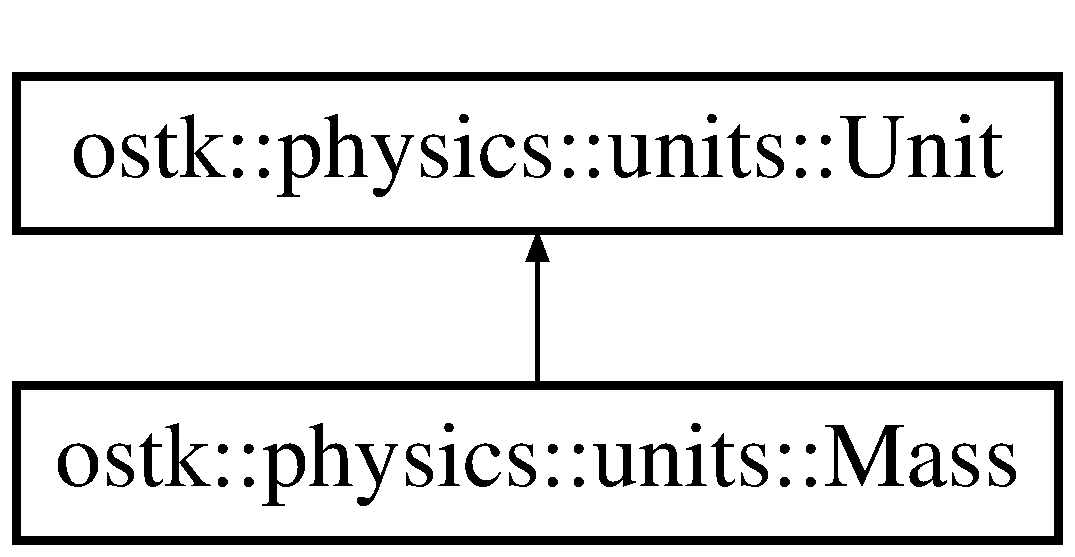
\includegraphics[height=2.000000cm]{classostk_1_1physics_1_1units_1_1_mass}
\end{center}
\end{figure}
\subsection*{Public Types}
\begin{DoxyCompactItemize}
\item 
enum \hyperlink{classostk_1_1physics_1_1units_1_1_mass_aa8994892478fdbe6dc78d4bca08db0fa}{Unit} \{ \hyperlink{classostk_1_1physics_1_1units_1_1_mass_aa8994892478fdbe6dc78d4bca08db0faaec0fc0100c4fc1ce4eea230c3dc10360}{Unit\+::\+Undefined}, 
\hyperlink{classostk_1_1physics_1_1units_1_1_mass_aa8994892478fdbe6dc78d4bca08db0faa9d71f8d145c74f11bf9b02047645bcf4}{Unit\+::\+Kilogram}, 
\hyperlink{classostk_1_1physics_1_1units_1_1_mass_aa8994892478fdbe6dc78d4bca08db0faa8cc4e66809c94072df6426c278d7b36b}{Unit\+::\+Tonne}, 
\hyperlink{classostk_1_1physics_1_1units_1_1_mass_aa8994892478fdbe6dc78d4bca08db0faa5a9dc6d94a5d29cbb1b5bc104fa23730}{Unit\+::\+Pound}
 \}
\end{DoxyCompactItemize}
\subsection*{Public Member Functions}
\begin{DoxyCompactItemize}
\item 
\hyperlink{classostk_1_1physics_1_1units_1_1_mass_a85999250131435a6d4116c826e93bfef}{Mass} (const Real \&a\+Value, const \hyperlink{classostk_1_1physics_1_1units_1_1_mass_aa8994892478fdbe6dc78d4bca08db0fa}{Mass\+::\+Unit} \&a\+Unit)
\begin{DoxyCompactList}\small\item\em Constructor. \end{DoxyCompactList}\item 
virtual \hyperlink{classostk_1_1physics_1_1units_1_1_mass}{Mass} $\ast$ \hyperlink{classostk_1_1physics_1_1units_1_1_mass_a1466c0c4860d94b0e6630476d4216033}{clone} () const override
\item 
virtual bool \hyperlink{classostk_1_1physics_1_1units_1_1_mass_ad6bb821365eff3a414d9fd07a7730d99}{is\+Defined} () const override
\item 
\hyperlink{classostk_1_1physics_1_1units_1_1_mass_aa8994892478fdbe6dc78d4bca08db0fa}{Mass\+::\+Unit} \hyperlink{classostk_1_1physics_1_1units_1_1_mass_a6ac920e7e64b09c39693a0837c070885}{get\+Unit} () const
\item 
Real \hyperlink{classostk_1_1physics_1_1units_1_1_mass_a4e337ca71db395510a6f6763bc356e9a}{in} (const \hyperlink{classostk_1_1physics_1_1units_1_1_mass_aa8994892478fdbe6dc78d4bca08db0fa}{Mass\+::\+Unit} \&a\+Unit) const
\item 
Real \hyperlink{classostk_1_1physics_1_1units_1_1_mass_a21d19ce58f97d3c96c95ccbdcaf7b216}{in\+Kilograms} () const
\item 
virtual String \hyperlink{classostk_1_1physics_1_1units_1_1_mass_aa8993fb7d2dbed494bbb68f8ec002af5}{to\+String} (const Integer \&a\+Precision=Integer\+::\+Undefined()) const override
\end{DoxyCompactItemize}
\subsection*{Static Public Member Functions}
\begin{DoxyCompactItemize}
\item 
static \hyperlink{classostk_1_1physics_1_1units_1_1_mass}{Mass} \hyperlink{classostk_1_1physics_1_1units_1_1_mass_a5ea55f35b93bcb681508bf51bcf21f1c}{Undefined} ()
\item 
static \hyperlink{classostk_1_1physics_1_1units_1_1_mass}{Mass} \hyperlink{classostk_1_1physics_1_1units_1_1_mass_aefe67261b5decb72bb9d753799aebc40}{Kilograms} (const Real \&a\+Value)
\item 
static \hyperlink{classostk_1_1physics_1_1units_1_1_mass}{Mass} \hyperlink{classostk_1_1physics_1_1units_1_1_mass_a1cdf07d3b4dba979b10c1a437c7f0f53}{Parse} (const String \&a\+String)
\item 
static String \hyperlink{classostk_1_1physics_1_1units_1_1_mass_a32be9ed18d39923f37346df6c63f4845}{String\+From\+Unit} (const \hyperlink{classostk_1_1physics_1_1units_1_1_mass_aa8994892478fdbe6dc78d4bca08db0fa}{Mass\+::\+Unit} \&a\+Unit)
\item 
static String \hyperlink{classostk_1_1physics_1_1units_1_1_mass_a2cbc7542169ae07850315f612cd60294}{Symbol\+From\+Unit} (const \hyperlink{classostk_1_1physics_1_1units_1_1_mass_aa8994892478fdbe6dc78d4bca08db0fa}{Mass\+::\+Unit} \&a\+Unit)
\end{DoxyCompactItemize}
\subsection*{Additional Inherited Members}


\subsection{Detailed Description}
\hyperlink{classostk_1_1physics_1_1units_1_1_mass}{Mass}. 

https\+://en.wikipedia.\+org/wiki/\+Mass 

\subsection{Member Enumeration Documentation}
\mbox{\Hypertarget{classostk_1_1physics_1_1units_1_1_mass_aa8994892478fdbe6dc78d4bca08db0fa}\label{classostk_1_1physics_1_1units_1_1_mass_aa8994892478fdbe6dc78d4bca08db0fa}} 
\index{ostk\+::physics\+::units\+::\+Mass@{ostk\+::physics\+::units\+::\+Mass}!Unit@{Unit}}
\index{Unit@{Unit}!ostk\+::physics\+::units\+::\+Mass@{ostk\+::physics\+::units\+::\+Mass}}
\subsubsection{\texorpdfstring{Unit}{Unit}}
{\footnotesize\ttfamily enum \hyperlink{classostk_1_1physics_1_1units_1_1_mass_aa8994892478fdbe6dc78d4bca08db0fa}{ostk\+::physics\+::units\+::\+Mass\+::\+Unit}\hspace{0.3cm}{\ttfamily [strong]}}

\begin{DoxyEnumFields}{Enumerator}
\raisebox{\heightof{T}}[0pt][0pt]{\index{Undefined@{Undefined}!ostk\+::physics\+::units\+::\+Mass@{ostk\+::physics\+::units\+::\+Mass}}\index{ostk\+::physics\+::units\+::\+Mass@{ostk\+::physics\+::units\+::\+Mass}!Undefined@{Undefined}}}\mbox{\Hypertarget{classostk_1_1physics_1_1units_1_1_mass_aa8994892478fdbe6dc78d4bca08db0faaec0fc0100c4fc1ce4eea230c3dc10360}\label{classostk_1_1physics_1_1units_1_1_mass_aa8994892478fdbe6dc78d4bca08db0faaec0fc0100c4fc1ce4eea230c3dc10360}} 
Undefined&Undefined. \\
\hline

\raisebox{\heightof{T}}[0pt][0pt]{\index{Kilogram@{Kilogram}!ostk\+::physics\+::units\+::\+Mass@{ostk\+::physics\+::units\+::\+Mass}}\index{ostk\+::physics\+::units\+::\+Mass@{ostk\+::physics\+::units\+::\+Mass}!Kilogram@{Kilogram}}}\mbox{\Hypertarget{classostk_1_1physics_1_1units_1_1_mass_aa8994892478fdbe6dc78d4bca08db0faa9d71f8d145c74f11bf9b02047645bcf4}\label{classostk_1_1physics_1_1units_1_1_mass_aa8994892478fdbe6dc78d4bca08db0faa9d71f8d145c74f11bf9b02047645bcf4}} 
Kilogram&Kilogram (SI) \\
\hline

\raisebox{\heightof{T}}[0pt][0pt]{\index{Tonne@{Tonne}!ostk\+::physics\+::units\+::\+Mass@{ostk\+::physics\+::units\+::\+Mass}}\index{ostk\+::physics\+::units\+::\+Mass@{ostk\+::physics\+::units\+::\+Mass}!Tonne@{Tonne}}}\mbox{\Hypertarget{classostk_1_1physics_1_1units_1_1_mass_aa8994892478fdbe6dc78d4bca08db0faa8cc4e66809c94072df6426c278d7b36b}\label{classostk_1_1physics_1_1units_1_1_mass_aa8994892478fdbe6dc78d4bca08db0faa8cc4e66809c94072df6426c278d7b36b}} 
Tonne&Tonne. \\
\hline

\raisebox{\heightof{T}}[0pt][0pt]{\index{Pound@{Pound}!ostk\+::physics\+::units\+::\+Mass@{ostk\+::physics\+::units\+::\+Mass}}\index{ostk\+::physics\+::units\+::\+Mass@{ostk\+::physics\+::units\+::\+Mass}!Pound@{Pound}}}\mbox{\Hypertarget{classostk_1_1physics_1_1units_1_1_mass_aa8994892478fdbe6dc78d4bca08db0faa5a9dc6d94a5d29cbb1b5bc104fa23730}\label{classostk_1_1physics_1_1units_1_1_mass_aa8994892478fdbe6dc78d4bca08db0faa5a9dc6d94a5d29cbb1b5bc104fa23730}} 
Pound&Pound. \\
\hline

\end{DoxyEnumFields}


\subsection{Constructor \& Destructor Documentation}
\mbox{\Hypertarget{classostk_1_1physics_1_1units_1_1_mass_a85999250131435a6d4116c826e93bfef}\label{classostk_1_1physics_1_1units_1_1_mass_a85999250131435a6d4116c826e93bfef}} 
\index{ostk\+::physics\+::units\+::\+Mass@{ostk\+::physics\+::units\+::\+Mass}!Mass@{Mass}}
\index{Mass@{Mass}!ostk\+::physics\+::units\+::\+Mass@{ostk\+::physics\+::units\+::\+Mass}}
\subsubsection{\texorpdfstring{Mass()}{Mass()}}
{\footnotesize\ttfamily ostk\+::physics\+::units\+::\+Mass\+::\+Mass (\begin{DoxyParamCaption}\item[{const Real \&}]{a\+Value,  }\item[{const \hyperlink{classostk_1_1physics_1_1units_1_1_mass_aa8994892478fdbe6dc78d4bca08db0fa}{Mass\+::\+Unit} \&}]{a\+Unit }\end{DoxyParamCaption})}



Constructor. 


\begin{DoxyCode}
\hyperlink{classostk_1_1physics_1_1units_1_1_mass_a85999250131435a6d4116c826e93bfef}{Mass} mass(1.0, \hyperlink{classostk_1_1physics_1_1units_1_1_mass_aa8994892478fdbe6dc78d4bca08db0faa9d71f8d145c74f11bf9b02047645bcf4}{Mass::Unit::Kilogram}) ;
\end{DoxyCode}



\begin{DoxyParams}[1]{Parameters}
\mbox{\tt in}  & {\em a\+Value} & A value \\
\hline
\mbox{\tt in}  & {\em a\+Unit} & A mass unit \\
\hline
\end{DoxyParams}


\subsection{Member Function Documentation}
\mbox{\Hypertarget{classostk_1_1physics_1_1units_1_1_mass_a1466c0c4860d94b0e6630476d4216033}\label{classostk_1_1physics_1_1units_1_1_mass_a1466c0c4860d94b0e6630476d4216033}} 
\index{ostk\+::physics\+::units\+::\+Mass@{ostk\+::physics\+::units\+::\+Mass}!clone@{clone}}
\index{clone@{clone}!ostk\+::physics\+::units\+::\+Mass@{ostk\+::physics\+::units\+::\+Mass}}
\subsubsection{\texorpdfstring{clone()}{clone()}}
{\footnotesize\ttfamily \hyperlink{classostk_1_1physics_1_1units_1_1_mass}{Mass} $\ast$ ostk\+::physics\+::units\+::\+Mass\+::clone (\begin{DoxyParamCaption}{ }\end{DoxyParamCaption}) const\hspace{0.3cm}{\ttfamily [override]}, {\ttfamily [virtual]}}



Implements \hyperlink{classostk_1_1physics_1_1units_1_1_unit_ab203628f8a16b16c28d89eaa4c3aff67}{ostk\+::physics\+::units\+::\+Unit}.

\mbox{\Hypertarget{classostk_1_1physics_1_1units_1_1_mass_a6ac920e7e64b09c39693a0837c070885}\label{classostk_1_1physics_1_1units_1_1_mass_a6ac920e7e64b09c39693a0837c070885}} 
\index{ostk\+::physics\+::units\+::\+Mass@{ostk\+::physics\+::units\+::\+Mass}!get\+Unit@{get\+Unit}}
\index{get\+Unit@{get\+Unit}!ostk\+::physics\+::units\+::\+Mass@{ostk\+::physics\+::units\+::\+Mass}}
\subsubsection{\texorpdfstring{get\+Unit()}{getUnit()}}
{\footnotesize\ttfamily \hyperlink{classostk_1_1physics_1_1units_1_1_mass_aa8994892478fdbe6dc78d4bca08db0fa}{Mass\+::\+Unit} ostk\+::physics\+::units\+::\+Mass\+::get\+Unit (\begin{DoxyParamCaption}{ }\end{DoxyParamCaption}) const}

\mbox{\Hypertarget{classostk_1_1physics_1_1units_1_1_mass_a4e337ca71db395510a6f6763bc356e9a}\label{classostk_1_1physics_1_1units_1_1_mass_a4e337ca71db395510a6f6763bc356e9a}} 
\index{ostk\+::physics\+::units\+::\+Mass@{ostk\+::physics\+::units\+::\+Mass}!in@{in}}
\index{in@{in}!ostk\+::physics\+::units\+::\+Mass@{ostk\+::physics\+::units\+::\+Mass}}
\subsubsection{\texorpdfstring{in()}{in()}}
{\footnotesize\ttfamily Real ostk\+::physics\+::units\+::\+Mass\+::in (\begin{DoxyParamCaption}\item[{const \hyperlink{classostk_1_1physics_1_1units_1_1_mass_aa8994892478fdbe6dc78d4bca08db0fa}{Mass\+::\+Unit} \&}]{a\+Unit }\end{DoxyParamCaption}) const}

\mbox{\Hypertarget{classostk_1_1physics_1_1units_1_1_mass_a21d19ce58f97d3c96c95ccbdcaf7b216}\label{classostk_1_1physics_1_1units_1_1_mass_a21d19ce58f97d3c96c95ccbdcaf7b216}} 
\index{ostk\+::physics\+::units\+::\+Mass@{ostk\+::physics\+::units\+::\+Mass}!in\+Kilograms@{in\+Kilograms}}
\index{in\+Kilograms@{in\+Kilograms}!ostk\+::physics\+::units\+::\+Mass@{ostk\+::physics\+::units\+::\+Mass}}
\subsubsection{\texorpdfstring{in\+Kilograms()}{inKilograms()}}
{\footnotesize\ttfamily Real ostk\+::physics\+::units\+::\+Mass\+::in\+Kilograms (\begin{DoxyParamCaption}{ }\end{DoxyParamCaption}) const}

\mbox{\Hypertarget{classostk_1_1physics_1_1units_1_1_mass_ad6bb821365eff3a414d9fd07a7730d99}\label{classostk_1_1physics_1_1units_1_1_mass_ad6bb821365eff3a414d9fd07a7730d99}} 
\index{ostk\+::physics\+::units\+::\+Mass@{ostk\+::physics\+::units\+::\+Mass}!is\+Defined@{is\+Defined}}
\index{is\+Defined@{is\+Defined}!ostk\+::physics\+::units\+::\+Mass@{ostk\+::physics\+::units\+::\+Mass}}
\subsubsection{\texorpdfstring{is\+Defined()}{isDefined()}}
{\footnotesize\ttfamily bool ostk\+::physics\+::units\+::\+Mass\+::is\+Defined (\begin{DoxyParamCaption}{ }\end{DoxyParamCaption}) const\hspace{0.3cm}{\ttfamily [override]}, {\ttfamily [virtual]}}



Reimplemented from \hyperlink{classostk_1_1physics_1_1units_1_1_unit_a423ce1df3478f0892b10824b591ae1cc}{ostk\+::physics\+::units\+::\+Unit}.

\mbox{\Hypertarget{classostk_1_1physics_1_1units_1_1_mass_aefe67261b5decb72bb9d753799aebc40}\label{classostk_1_1physics_1_1units_1_1_mass_aefe67261b5decb72bb9d753799aebc40}} 
\index{ostk\+::physics\+::units\+::\+Mass@{ostk\+::physics\+::units\+::\+Mass}!Kilograms@{Kilograms}}
\index{Kilograms@{Kilograms}!ostk\+::physics\+::units\+::\+Mass@{ostk\+::physics\+::units\+::\+Mass}}
\subsubsection{\texorpdfstring{Kilograms()}{Kilograms()}}
{\footnotesize\ttfamily \hyperlink{classostk_1_1physics_1_1units_1_1_mass}{Mass} ostk\+::physics\+::units\+::\+Mass\+::\+Kilograms (\begin{DoxyParamCaption}\item[{const Real \&}]{a\+Value }\end{DoxyParamCaption})\hspace{0.3cm}{\ttfamily [static]}}

\mbox{\Hypertarget{classostk_1_1physics_1_1units_1_1_mass_a1cdf07d3b4dba979b10c1a437c7f0f53}\label{classostk_1_1physics_1_1units_1_1_mass_a1cdf07d3b4dba979b10c1a437c7f0f53}} 
\index{ostk\+::physics\+::units\+::\+Mass@{ostk\+::physics\+::units\+::\+Mass}!Parse@{Parse}}
\index{Parse@{Parse}!ostk\+::physics\+::units\+::\+Mass@{ostk\+::physics\+::units\+::\+Mass}}
\subsubsection{\texorpdfstring{Parse()}{Parse()}}
{\footnotesize\ttfamily static \hyperlink{classostk_1_1physics_1_1units_1_1_mass}{Mass} ostk\+::physics\+::units\+::\+Mass\+::\+Parse (\begin{DoxyParamCaption}\item[{const String \&}]{a\+String }\end{DoxyParamCaption})\hspace{0.3cm}{\ttfamily [static]}}

\mbox{\Hypertarget{classostk_1_1physics_1_1units_1_1_mass_a32be9ed18d39923f37346df6c63f4845}\label{classostk_1_1physics_1_1units_1_1_mass_a32be9ed18d39923f37346df6c63f4845}} 
\index{ostk\+::physics\+::units\+::\+Mass@{ostk\+::physics\+::units\+::\+Mass}!String\+From\+Unit@{String\+From\+Unit}}
\index{String\+From\+Unit@{String\+From\+Unit}!ostk\+::physics\+::units\+::\+Mass@{ostk\+::physics\+::units\+::\+Mass}}
\subsubsection{\texorpdfstring{String\+From\+Unit()}{StringFromUnit()}}
{\footnotesize\ttfamily String ostk\+::physics\+::units\+::\+Mass\+::\+String\+From\+Unit (\begin{DoxyParamCaption}\item[{const \hyperlink{classostk_1_1physics_1_1units_1_1_mass_aa8994892478fdbe6dc78d4bca08db0fa}{Mass\+::\+Unit} \&}]{a\+Unit }\end{DoxyParamCaption})\hspace{0.3cm}{\ttfamily [static]}}

\mbox{\Hypertarget{classostk_1_1physics_1_1units_1_1_mass_a2cbc7542169ae07850315f612cd60294}\label{classostk_1_1physics_1_1units_1_1_mass_a2cbc7542169ae07850315f612cd60294}} 
\index{ostk\+::physics\+::units\+::\+Mass@{ostk\+::physics\+::units\+::\+Mass}!Symbol\+From\+Unit@{Symbol\+From\+Unit}}
\index{Symbol\+From\+Unit@{Symbol\+From\+Unit}!ostk\+::physics\+::units\+::\+Mass@{ostk\+::physics\+::units\+::\+Mass}}
\subsubsection{\texorpdfstring{Symbol\+From\+Unit()}{SymbolFromUnit()}}
{\footnotesize\ttfamily String ostk\+::physics\+::units\+::\+Mass\+::\+Symbol\+From\+Unit (\begin{DoxyParamCaption}\item[{const \hyperlink{classostk_1_1physics_1_1units_1_1_mass_aa8994892478fdbe6dc78d4bca08db0fa}{Mass\+::\+Unit} \&}]{a\+Unit }\end{DoxyParamCaption})\hspace{0.3cm}{\ttfamily [static]}}

\mbox{\Hypertarget{classostk_1_1physics_1_1units_1_1_mass_aa8993fb7d2dbed494bbb68f8ec002af5}\label{classostk_1_1physics_1_1units_1_1_mass_aa8993fb7d2dbed494bbb68f8ec002af5}} 
\index{ostk\+::physics\+::units\+::\+Mass@{ostk\+::physics\+::units\+::\+Mass}!to\+String@{to\+String}}
\index{to\+String@{to\+String}!ostk\+::physics\+::units\+::\+Mass@{ostk\+::physics\+::units\+::\+Mass}}
\subsubsection{\texorpdfstring{to\+String()}{toString()}}
{\footnotesize\ttfamily String ostk\+::physics\+::units\+::\+Mass\+::to\+String (\begin{DoxyParamCaption}\item[{const Integer \&}]{a\+Precision = {\ttfamily Integer\+:\+:Undefined()} }\end{DoxyParamCaption}) const\hspace{0.3cm}{\ttfamily [override]}, {\ttfamily [virtual]}}



Implements \hyperlink{classostk_1_1physics_1_1units_1_1_unit_a8162b4eb8221c7577af16ab8b399d07e}{ostk\+::physics\+::units\+::\+Unit}.

\mbox{\Hypertarget{classostk_1_1physics_1_1units_1_1_mass_a5ea55f35b93bcb681508bf51bcf21f1c}\label{classostk_1_1physics_1_1units_1_1_mass_a5ea55f35b93bcb681508bf51bcf21f1c}} 
\index{ostk\+::physics\+::units\+::\+Mass@{ostk\+::physics\+::units\+::\+Mass}!Undefined@{Undefined}}
\index{Undefined@{Undefined}!ostk\+::physics\+::units\+::\+Mass@{ostk\+::physics\+::units\+::\+Mass}}
\subsubsection{\texorpdfstring{Undefined()}{Undefined()}}
{\footnotesize\ttfamily \hyperlink{classostk_1_1physics_1_1units_1_1_mass}{Mass} ostk\+::physics\+::units\+::\+Mass\+::\+Undefined (\begin{DoxyParamCaption}{ }\end{DoxyParamCaption})\hspace{0.3cm}{\ttfamily [static]}}



The documentation for this class was generated from the following files\+:\begin{DoxyCompactItemize}
\item 
include/\+Open\+Space\+Toolkit/\+Physics/\+Units/\hyperlink{_mass_8hpp}{Mass.\+hpp}\item 
src/\+Open\+Space\+Toolkit/\+Physics/\+Units/\hyperlink{_mass_8cpp}{Mass.\+cpp}\end{DoxyCompactItemize}

\hypertarget{classostk_1_1physics_1_1environment_1_1magnetic_1_1_model}{}\section{ostk\+:\+:physics\+:\+:environment\+:\+:magnetic\+:\+:Model Class Reference}
\label{classostk_1_1physics_1_1environment_1_1magnetic_1_1_model}\index{ostk\+::physics\+::environment\+::magnetic\+::\+Model@{ostk\+::physics\+::environment\+::magnetic\+::\+Model}}


Magnetic model (interface)  




{\ttfamily \#include $<$Model.\+hpp$>$}

Inheritance diagram for ostk\+:\+:physics\+:\+:environment\+:\+:magnetic\+:\+:Model\+:\begin{figure}[H]
\begin{center}
\leavevmode
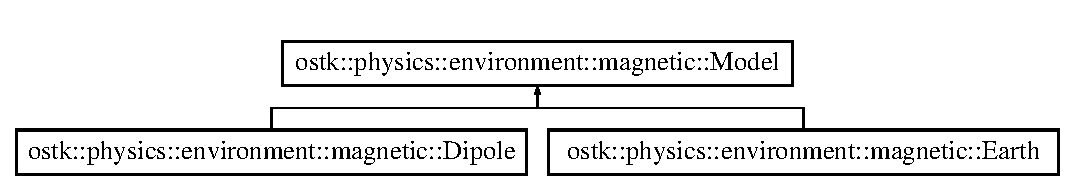
\includegraphics[height=2.000000cm]{classostk_1_1physics_1_1environment_1_1magnetic_1_1_model}
\end{center}
\end{figure}
\subsection*{Public Member Functions}
\begin{DoxyCompactItemize}
\item 
\hyperlink{classostk_1_1physics_1_1environment_1_1magnetic_1_1_model_a50d6421402d4f67aa9c45e9be5f27d30}{Model} ()
\begin{DoxyCompactList}\small\item\em Constructor (default) \end{DoxyCompactList}\item 
virtual \hyperlink{classostk_1_1physics_1_1environment_1_1magnetic_1_1_model_a6fe1b73447dc65989d31db636fa73953}{$\sim$\+Model} ()=0
\begin{DoxyCompactList}\small\item\em Destructor (pure virtual) \end{DoxyCompactList}\item 
virtual \hyperlink{classostk_1_1physics_1_1environment_1_1magnetic_1_1_model}{Model} $\ast$ \hyperlink{classostk_1_1physics_1_1environment_1_1magnetic_1_1_model_af357908c151a7809bbbc8fc676bd07b6}{clone} () const =0
\begin{DoxyCompactList}\small\item\em Clone the magnetic model (pure virtual) \end{DoxyCompactList}\item 
virtual Vector3d \hyperlink{classostk_1_1physics_1_1environment_1_1magnetic_1_1_model_abf0510f9be2c196ea3c0586d02979b0f}{get\+Field\+Value\+At} (const Vector3d \&a\+Position, const \hyperlink{classostk_1_1physics_1_1time_1_1_instant}{Instant} \&an\+Instant) const =0
\begin{DoxyCompactList}\small\item\em Get the magnetic field value at a given position and instant (pure virtual) \end{DoxyCompactList}\end{DoxyCompactItemize}


\subsection{Detailed Description}
Magnetic model (interface) 

\subsection{Constructor \& Destructor Documentation}
\mbox{\Hypertarget{classostk_1_1physics_1_1environment_1_1magnetic_1_1_model_a50d6421402d4f67aa9c45e9be5f27d30}\label{classostk_1_1physics_1_1environment_1_1magnetic_1_1_model_a50d6421402d4f67aa9c45e9be5f27d30}} 
\index{ostk\+::physics\+::environment\+::magnetic\+::\+Model@{ostk\+::physics\+::environment\+::magnetic\+::\+Model}!Model@{Model}}
\index{Model@{Model}!ostk\+::physics\+::environment\+::magnetic\+::\+Model@{ostk\+::physics\+::environment\+::magnetic\+::\+Model}}
\subsubsection{\texorpdfstring{Model()}{Model()}}
{\footnotesize\ttfamily ostk\+::physics\+::environment\+::magnetic\+::\+Model\+::\+Model (\begin{DoxyParamCaption}{ }\end{DoxyParamCaption})}



Constructor (default) 

\mbox{\Hypertarget{classostk_1_1physics_1_1environment_1_1magnetic_1_1_model_a6fe1b73447dc65989d31db636fa73953}\label{classostk_1_1physics_1_1environment_1_1magnetic_1_1_model_a6fe1b73447dc65989d31db636fa73953}} 
\index{ostk\+::physics\+::environment\+::magnetic\+::\+Model@{ostk\+::physics\+::environment\+::magnetic\+::\+Model}!````~Model@{$\sim$\+Model}}
\index{````~Model@{$\sim$\+Model}!ostk\+::physics\+::environment\+::magnetic\+::\+Model@{ostk\+::physics\+::environment\+::magnetic\+::\+Model}}
\subsubsection{\texorpdfstring{$\sim$\+Model()}{~Model()}}
{\footnotesize\ttfamily ostk\+::physics\+::environment\+::magnetic\+::\+Model\+::$\sim$\+Model (\begin{DoxyParamCaption}{ }\end{DoxyParamCaption})\hspace{0.3cm}{\ttfamily [pure virtual]}}



Destructor (pure virtual) 



\subsection{Member Function Documentation}
\mbox{\Hypertarget{classostk_1_1physics_1_1environment_1_1magnetic_1_1_model_af357908c151a7809bbbc8fc676bd07b6}\label{classostk_1_1physics_1_1environment_1_1magnetic_1_1_model_af357908c151a7809bbbc8fc676bd07b6}} 
\index{ostk\+::physics\+::environment\+::magnetic\+::\+Model@{ostk\+::physics\+::environment\+::magnetic\+::\+Model}!clone@{clone}}
\index{clone@{clone}!ostk\+::physics\+::environment\+::magnetic\+::\+Model@{ostk\+::physics\+::environment\+::magnetic\+::\+Model}}
\subsubsection{\texorpdfstring{clone()}{clone()}}
{\footnotesize\ttfamily virtual \hyperlink{classostk_1_1physics_1_1environment_1_1magnetic_1_1_model}{Model}$\ast$ ostk\+::physics\+::environment\+::magnetic\+::\+Model\+::clone (\begin{DoxyParamCaption}{ }\end{DoxyParamCaption}) const\hspace{0.3cm}{\ttfamily [pure virtual]}}



Clone the magnetic model (pure virtual) 

\begin{DoxyReturn}{Returns}
Pointer to magnetic model 
\end{DoxyReturn}


Implemented in \hyperlink{classostk_1_1physics_1_1environment_1_1magnetic_1_1_earth_ac4b57f94304595595fc3eebb0dd0d050}{ostk\+::physics\+::environment\+::magnetic\+::\+Earth}, and \hyperlink{classostk_1_1physics_1_1environment_1_1magnetic_1_1_dipole_ad4255ff1007a339c9f0bdbda321c0ab2}{ostk\+::physics\+::environment\+::magnetic\+::\+Dipole}.

\mbox{\Hypertarget{classostk_1_1physics_1_1environment_1_1magnetic_1_1_model_abf0510f9be2c196ea3c0586d02979b0f}\label{classostk_1_1physics_1_1environment_1_1magnetic_1_1_model_abf0510f9be2c196ea3c0586d02979b0f}} 
\index{ostk\+::physics\+::environment\+::magnetic\+::\+Model@{ostk\+::physics\+::environment\+::magnetic\+::\+Model}!get\+Field\+Value\+At@{get\+Field\+Value\+At}}
\index{get\+Field\+Value\+At@{get\+Field\+Value\+At}!ostk\+::physics\+::environment\+::magnetic\+::\+Model@{ostk\+::physics\+::environment\+::magnetic\+::\+Model}}
\subsubsection{\texorpdfstring{get\+Field\+Value\+At()}{getFieldValueAt()}}
{\footnotesize\ttfamily virtual Vector3d ostk\+::physics\+::environment\+::magnetic\+::\+Model\+::get\+Field\+Value\+At (\begin{DoxyParamCaption}\item[{const Vector3d \&}]{a\+Position,  }\item[{const \hyperlink{classostk_1_1physics_1_1time_1_1_instant}{Instant} \&}]{an\+Instant }\end{DoxyParamCaption}) const\hspace{0.3cm}{\ttfamily [pure virtual]}}



Get the magnetic field value at a given position and instant (pure virtual) 


\begin{DoxyParams}[1]{Parameters}
\mbox{\tt in}  & {\em a\+Position} & A position, expressed in the magnetic object frame \mbox{[}m\mbox{]} \\
\hline
\mbox{\tt in}  & {\em an\+Instant} & An instant \\
\hline
\end{DoxyParams}
\begin{DoxyReturn}{Returns}
Magnetic field value, expressed in the magnetic object frame \mbox{[}T\mbox{]} 
\end{DoxyReturn}


Implemented in \hyperlink{classostk_1_1physics_1_1environment_1_1magnetic_1_1_earth_a2f39ff75c4a674b6720b27c2c6a0b930}{ostk\+::physics\+::environment\+::magnetic\+::\+Earth}, and \hyperlink{classostk_1_1physics_1_1environment_1_1magnetic_1_1_dipole_ae2c65e41445c91b3efec455fb5077ab1}{ostk\+::physics\+::environment\+::magnetic\+::\+Dipole}.



The documentation for this class was generated from the following files\+:\begin{DoxyCompactItemize}
\item 
include/\+Open\+Space\+Toolkit/\+Physics/\+Environment/\+Magnetic/\hyperlink{_magnetic_2_model_8hpp}{Model.\+hpp}\item 
src/\+Open\+Space\+Toolkit/\+Physics/\+Environment/\+Magnetic/\hyperlink{_magnetic_2_model_8cpp}{Model.\+cpp}\end{DoxyCompactItemize}

\hypertarget{classostk_1_1physics_1_1environment_1_1gravitational_1_1_model}{}\section{ostk\+:\+:physics\+:\+:environment\+:\+:gravitational\+:\+:Model Class Reference}
\label{classostk_1_1physics_1_1environment_1_1gravitational_1_1_model}\index{ostk\+::physics\+::environment\+::gravitational\+::\+Model@{ostk\+::physics\+::environment\+::gravitational\+::\+Model}}


Gravitational model (interface)  




{\ttfamily \#include $<$Model.\+hpp$>$}

Inheritance diagram for ostk\+:\+:physics\+:\+:environment\+:\+:gravitational\+:\+:Model\+:\begin{figure}[H]
\begin{center}
\leavevmode
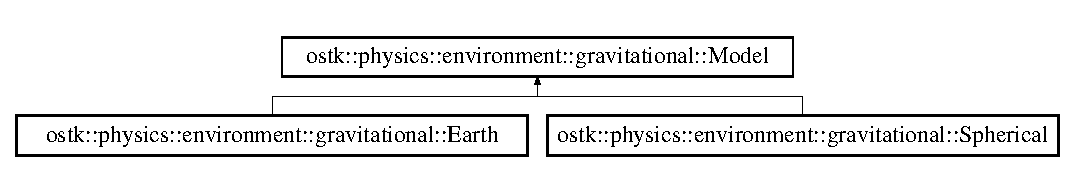
\includegraphics[height=1.860465cm]{classostk_1_1physics_1_1environment_1_1gravitational_1_1_model}
\end{center}
\end{figure}
\subsection*{Public Member Functions}
\begin{DoxyCompactItemize}
\item 
\hyperlink{classostk_1_1physics_1_1environment_1_1gravitational_1_1_model_ad588a72265bacd216b6d3b19d4736ae9}{Model} ()
\begin{DoxyCompactList}\small\item\em Constructor (default) \end{DoxyCompactList}\item 
virtual \hyperlink{classostk_1_1physics_1_1environment_1_1gravitational_1_1_model_ab44f53d6e046fb5d436b90128aff0850}{$\sim$\+Model} ()=0
\begin{DoxyCompactList}\small\item\em Destructor (pure virtual) \end{DoxyCompactList}\item 
virtual \hyperlink{classostk_1_1physics_1_1environment_1_1gravitational_1_1_model}{Model} $\ast$ \hyperlink{classostk_1_1physics_1_1environment_1_1gravitational_1_1_model_a399257ac86e7f0112a702141e0e2e4a7}{clone} () const =0
\begin{DoxyCompactList}\small\item\em Clone the gravitational model (pure virtual) \end{DoxyCompactList}\item 
virtual Vector3d \hyperlink{classostk_1_1physics_1_1environment_1_1gravitational_1_1_model_a5ef3b4ddf4240e8a26553294fe392581}{get\+Field\+Value\+At} (const Vector3d \&a\+Position, const \hyperlink{classostk_1_1physics_1_1time_1_1_instant}{Instant} \&an\+Instant) const =0
\begin{DoxyCompactList}\small\item\em Get the gravitational field value at a given position and instant (pure virtual) \end{DoxyCompactList}\end{DoxyCompactItemize}


\subsection{Detailed Description}
Gravitational model (interface) 

\subsection{Constructor \& Destructor Documentation}
\mbox{\Hypertarget{classostk_1_1physics_1_1environment_1_1gravitational_1_1_model_ad588a72265bacd216b6d3b19d4736ae9}\label{classostk_1_1physics_1_1environment_1_1gravitational_1_1_model_ad588a72265bacd216b6d3b19d4736ae9}} 
\index{ostk\+::physics\+::environment\+::gravitational\+::\+Model@{ostk\+::physics\+::environment\+::gravitational\+::\+Model}!Model@{Model}}
\index{Model@{Model}!ostk\+::physics\+::environment\+::gravitational\+::\+Model@{ostk\+::physics\+::environment\+::gravitational\+::\+Model}}
\subsubsection{\texorpdfstring{Model()}{Model()}}
{\footnotesize\ttfamily ostk\+::physics\+::environment\+::gravitational\+::\+Model\+::\+Model (\begin{DoxyParamCaption}{ }\end{DoxyParamCaption})}



Constructor (default) 

\mbox{\Hypertarget{classostk_1_1physics_1_1environment_1_1gravitational_1_1_model_ab44f53d6e046fb5d436b90128aff0850}\label{classostk_1_1physics_1_1environment_1_1gravitational_1_1_model_ab44f53d6e046fb5d436b90128aff0850}} 
\index{ostk\+::physics\+::environment\+::gravitational\+::\+Model@{ostk\+::physics\+::environment\+::gravitational\+::\+Model}!````~Model@{$\sim$\+Model}}
\index{````~Model@{$\sim$\+Model}!ostk\+::physics\+::environment\+::gravitational\+::\+Model@{ostk\+::physics\+::environment\+::gravitational\+::\+Model}}
\subsubsection{\texorpdfstring{$\sim$\+Model()}{~Model()}}
{\footnotesize\ttfamily ostk\+::physics\+::environment\+::gravitational\+::\+Model\+::$\sim$\+Model (\begin{DoxyParamCaption}{ }\end{DoxyParamCaption})\hspace{0.3cm}{\ttfamily [pure virtual]}}



Destructor (pure virtual) 



\subsection{Member Function Documentation}
\mbox{\Hypertarget{classostk_1_1physics_1_1environment_1_1gravitational_1_1_model_a399257ac86e7f0112a702141e0e2e4a7}\label{classostk_1_1physics_1_1environment_1_1gravitational_1_1_model_a399257ac86e7f0112a702141e0e2e4a7}} 
\index{ostk\+::physics\+::environment\+::gravitational\+::\+Model@{ostk\+::physics\+::environment\+::gravitational\+::\+Model}!clone@{clone}}
\index{clone@{clone}!ostk\+::physics\+::environment\+::gravitational\+::\+Model@{ostk\+::physics\+::environment\+::gravitational\+::\+Model}}
\subsubsection{\texorpdfstring{clone()}{clone()}}
{\footnotesize\ttfamily virtual \hyperlink{classostk_1_1physics_1_1environment_1_1gravitational_1_1_model}{Model}$\ast$ ostk\+::physics\+::environment\+::gravitational\+::\+Model\+::clone (\begin{DoxyParamCaption}{ }\end{DoxyParamCaption}) const\hspace{0.3cm}{\ttfamily [pure virtual]}}



Clone the gravitational model (pure virtual) 

\begin{DoxyReturn}{Returns}
Pointer to gravitational model 
\end{DoxyReturn}


Implemented in \hyperlink{classostk_1_1physics_1_1environment_1_1gravitational_1_1_earth_a987c2df62d8fedb368acf37e71ba7a47}{ostk\+::physics\+::environment\+::gravitational\+::\+Earth}, and \hyperlink{classostk_1_1physics_1_1environment_1_1gravitational_1_1_spherical_ac9f63de9656589a27a77e7a8d48836bd}{ostk\+::physics\+::environment\+::gravitational\+::\+Spherical}.

\mbox{\Hypertarget{classostk_1_1physics_1_1environment_1_1gravitational_1_1_model_a5ef3b4ddf4240e8a26553294fe392581}\label{classostk_1_1physics_1_1environment_1_1gravitational_1_1_model_a5ef3b4ddf4240e8a26553294fe392581}} 
\index{ostk\+::physics\+::environment\+::gravitational\+::\+Model@{ostk\+::physics\+::environment\+::gravitational\+::\+Model}!get\+Field\+Value\+At@{get\+Field\+Value\+At}}
\index{get\+Field\+Value\+At@{get\+Field\+Value\+At}!ostk\+::physics\+::environment\+::gravitational\+::\+Model@{ostk\+::physics\+::environment\+::gravitational\+::\+Model}}
\subsubsection{\texorpdfstring{get\+Field\+Value\+At()}{getFieldValueAt()}}
{\footnotesize\ttfamily virtual Vector3d ostk\+::physics\+::environment\+::gravitational\+::\+Model\+::get\+Field\+Value\+At (\begin{DoxyParamCaption}\item[{const Vector3d \&}]{a\+Position,  }\item[{const \hyperlink{classostk_1_1physics_1_1time_1_1_instant}{Instant} \&}]{an\+Instant }\end{DoxyParamCaption}) const\hspace{0.3cm}{\ttfamily [pure virtual]}}



Get the gravitational field value at a given position and instant (pure virtual) 


\begin{DoxyParams}[1]{Parameters}
\mbox{\tt in}  & {\em a\+Position} & A position, expressed in the gravitational object frame \mbox{[}m\mbox{]} \\
\hline
\mbox{\tt in}  & {\em an\+Instant} & An instant \\
\hline
\end{DoxyParams}
\begin{DoxyReturn}{Returns}
Gravitational field value, expressed in the gravitational object frame \mbox{[}m.\+s-\/2\mbox{]} 
\end{DoxyReturn}


Implemented in \hyperlink{classostk_1_1physics_1_1environment_1_1gravitational_1_1_earth_a9e536649566761f4bdd467993abfcedd}{ostk\+::physics\+::environment\+::gravitational\+::\+Earth}, and \hyperlink{classostk_1_1physics_1_1environment_1_1gravitational_1_1_spherical_a37243cf671418b0cb9eff229101b5e96}{ostk\+::physics\+::environment\+::gravitational\+::\+Spherical}.



The documentation for this class was generated from the following files\+:\begin{DoxyCompactItemize}
\item 
include/\+Open\+Space\+Toolkit/\+Physics/\+Environment/\+Gravitational/\hyperlink{_gravitational_2_model_8hpp}{Model.\+hpp}\item 
src/\+Open\+Space\+Toolkit/\+Physics/\+Environment/\+Gravitational/\hyperlink{_gravitational_2_model_8cpp}{Model.\+cpp}\end{DoxyCompactItemize}

\hypertarget{structostk_1_1physics_1_1env_1_1obj_1_1_celestial_1_1_model_base}{}\section{ostk\+:\+:physics\+:\+:env\+:\+:obj\+:\+:Celestial\+:\+:Model\+Base Struct Reference}
\label{structostk_1_1physics_1_1env_1_1obj_1_1_celestial_1_1_model_base}\index{ostk\+::physics\+::env\+::obj\+::\+Celestial\+::\+Model\+Base@{ostk\+::physics\+::env\+::obj\+::\+Celestial\+::\+Model\+Base}}


{\ttfamily \#include $<$Celestial.\+hpp$>$}

\subsection*{Static Public Attributes}
\begin{DoxyCompactItemize}
\item 
static \hyperlink{classostk_1_1physics_1_1units_1_1_derived}{Derived} \hyperlink{structostk_1_1physics_1_1env_1_1obj_1_1_celestial_1_1_model_base_a4c56c7c4d2a9bb05f1ae77823638b900}{Gravitational\+Parameter}
\item 
static \hyperlink{classostk_1_1physics_1_1units_1_1_length}{Length} \hyperlink{structostk_1_1physics_1_1env_1_1obj_1_1_celestial_1_1_model_base_a38c0a47396e9cb47028ffbe09a464044}{Equatorial\+Radius}
\item 
static Real \hyperlink{structostk_1_1physics_1_1env_1_1obj_1_1_celestial_1_1_model_base_a6fd974f2c2691cb5c30a845a35cd346f}{Flattening}
\item 
static Real \hyperlink{structostk_1_1physics_1_1env_1_1obj_1_1_celestial_1_1_model_base_a6279947bed22b473663d3c508bd76a3e}{C20}
\item 
static Real \hyperlink{structostk_1_1physics_1_1env_1_1obj_1_1_celestial_1_1_model_base_a80c4de90c9b3c463dc194382fa2c028c}{J2}
\end{DoxyCompactItemize}


\subsection{Member Data Documentation}
\mbox{\Hypertarget{structostk_1_1physics_1_1env_1_1obj_1_1_celestial_1_1_model_base_a6279947bed22b473663d3c508bd76a3e}\label{structostk_1_1physics_1_1env_1_1obj_1_1_celestial_1_1_model_base_a6279947bed22b473663d3c508bd76a3e}} 
\index{ostk\+::physics\+::env\+::obj\+::\+Celestial\+::\+Model\+Base@{ostk\+::physics\+::env\+::obj\+::\+Celestial\+::\+Model\+Base}!C20@{C20}}
\index{C20@{C20}!ostk\+::physics\+::env\+::obj\+::\+Celestial\+::\+Model\+Base@{ostk\+::physics\+::env\+::obj\+::\+Celestial\+::\+Model\+Base}}
\subsubsection{\texorpdfstring{C20}{C20}}
{\footnotesize\ttfamily Real ostk\+::physics\+::env\+::obj\+::\+Celestial\+::\+Model\+Base\+::\+C20\hspace{0.3cm}{\ttfamily [static]}}

\mbox{\Hypertarget{structostk_1_1physics_1_1env_1_1obj_1_1_celestial_1_1_model_base_a38c0a47396e9cb47028ffbe09a464044}\label{structostk_1_1physics_1_1env_1_1obj_1_1_celestial_1_1_model_base_a38c0a47396e9cb47028ffbe09a464044}} 
\index{ostk\+::physics\+::env\+::obj\+::\+Celestial\+::\+Model\+Base@{ostk\+::physics\+::env\+::obj\+::\+Celestial\+::\+Model\+Base}!Equatorial\+Radius@{Equatorial\+Radius}}
\index{Equatorial\+Radius@{Equatorial\+Radius}!ostk\+::physics\+::env\+::obj\+::\+Celestial\+::\+Model\+Base@{ostk\+::physics\+::env\+::obj\+::\+Celestial\+::\+Model\+Base}}
\subsubsection{\texorpdfstring{Equatorial\+Radius}{EquatorialRadius}}
{\footnotesize\ttfamily \hyperlink{classostk_1_1physics_1_1units_1_1_length}{Length} ostk\+::physics\+::env\+::obj\+::\+Celestial\+::\+Model\+Base\+::\+Equatorial\+Radius\hspace{0.3cm}{\ttfamily [static]}}

\mbox{\Hypertarget{structostk_1_1physics_1_1env_1_1obj_1_1_celestial_1_1_model_base_a6fd974f2c2691cb5c30a845a35cd346f}\label{structostk_1_1physics_1_1env_1_1obj_1_1_celestial_1_1_model_base_a6fd974f2c2691cb5c30a845a35cd346f}} 
\index{ostk\+::physics\+::env\+::obj\+::\+Celestial\+::\+Model\+Base@{ostk\+::physics\+::env\+::obj\+::\+Celestial\+::\+Model\+Base}!Flattening@{Flattening}}
\index{Flattening@{Flattening}!ostk\+::physics\+::env\+::obj\+::\+Celestial\+::\+Model\+Base@{ostk\+::physics\+::env\+::obj\+::\+Celestial\+::\+Model\+Base}}
\subsubsection{\texorpdfstring{Flattening}{Flattening}}
{\footnotesize\ttfamily Real ostk\+::physics\+::env\+::obj\+::\+Celestial\+::\+Model\+Base\+::\+Flattening\hspace{0.3cm}{\ttfamily [static]}}

\mbox{\Hypertarget{structostk_1_1physics_1_1env_1_1obj_1_1_celestial_1_1_model_base_a4c56c7c4d2a9bb05f1ae77823638b900}\label{structostk_1_1physics_1_1env_1_1obj_1_1_celestial_1_1_model_base_a4c56c7c4d2a9bb05f1ae77823638b900}} 
\index{ostk\+::physics\+::env\+::obj\+::\+Celestial\+::\+Model\+Base@{ostk\+::physics\+::env\+::obj\+::\+Celestial\+::\+Model\+Base}!Gravitational\+Parameter@{Gravitational\+Parameter}}
\index{Gravitational\+Parameter@{Gravitational\+Parameter}!ostk\+::physics\+::env\+::obj\+::\+Celestial\+::\+Model\+Base@{ostk\+::physics\+::env\+::obj\+::\+Celestial\+::\+Model\+Base}}
\subsubsection{\texorpdfstring{Gravitational\+Parameter}{GravitationalParameter}}
{\footnotesize\ttfamily \hyperlink{classostk_1_1physics_1_1units_1_1_derived}{Derived} ostk\+::physics\+::env\+::obj\+::\+Celestial\+::\+Model\+Base\+::\+Gravitational\+Parameter\hspace{0.3cm}{\ttfamily [static]}}

\mbox{\Hypertarget{structostk_1_1physics_1_1env_1_1obj_1_1_celestial_1_1_model_base_a80c4de90c9b3c463dc194382fa2c028c}\label{structostk_1_1physics_1_1env_1_1obj_1_1_celestial_1_1_model_base_a80c4de90c9b3c463dc194382fa2c028c}} 
\index{ostk\+::physics\+::env\+::obj\+::\+Celestial\+::\+Model\+Base@{ostk\+::physics\+::env\+::obj\+::\+Celestial\+::\+Model\+Base}!J2@{J2}}
\index{J2@{J2}!ostk\+::physics\+::env\+::obj\+::\+Celestial\+::\+Model\+Base@{ostk\+::physics\+::env\+::obj\+::\+Celestial\+::\+Model\+Base}}
\subsubsection{\texorpdfstring{J2}{J2}}
{\footnotesize\ttfamily Real ostk\+::physics\+::env\+::obj\+::\+Celestial\+::\+Model\+Base\+::\+J2\hspace{0.3cm}{\ttfamily [static]}}



The documentation for this struct was generated from the following file\+:\begin{DoxyCompactItemize}
\item 
include/\+Open\+Space\+Toolkit/\+Physics/\+Environment/\+Objects/\hyperlink{_celestial_8hpp}{Celestial.\+hpp}\end{DoxyCompactItemize}

\hypertarget{structostk_1_1physics_1_1env_1_1obj_1_1celest_1_1_earth_1_1_models}{}\section{ostk\+:\+:physics\+:\+:env\+:\+:obj\+:\+:celest\+:\+:Earth\+:\+:Models Struct Reference}
\label{structostk_1_1physics_1_1env_1_1obj_1_1celest_1_1_earth_1_1_models}\index{ostk\+::physics\+::env\+::obj\+::celest\+::\+Earth\+::\+Models@{ostk\+::physics\+::env\+::obj\+::celest\+::\+Earth\+::\+Models}}


{\ttfamily \#include $<$Earth.\+hpp$>$}

\subsection*{Classes}
\begin{DoxyCompactItemize}
\item 
struct \hyperlink{structostk_1_1physics_1_1env_1_1obj_1_1celest_1_1_earth_1_1_models_1_1_e_g_m2008}{E\+G\+M2008}
\item 
struct \hyperlink{structostk_1_1physics_1_1env_1_1obj_1_1celest_1_1_earth_1_1_models_1_1_e_g_m96}{E\+G\+M96}
\item 
struct \hyperlink{structostk_1_1physics_1_1env_1_1obj_1_1celest_1_1_earth_1_1_models_1_1_w_g_s84}{W\+G\+S84}
\item 
struct \hyperlink{structostk_1_1physics_1_1env_1_1obj_1_1celest_1_1_earth_1_1_models_1_1_w_g_s84___e_g_m96}{W\+G\+S84\+\_\+\+E\+G\+M96}
\end{DoxyCompactItemize}


The documentation for this struct was generated from the following file\+:\begin{DoxyCompactItemize}
\item 
include/\+Open\+Space\+Toolkit/\+Physics/\+Environment/\+Objects/\+Celestial\+Bodies/\hyperlink{_objects_2_celestial_bodies_2_earth_8hpp}{Earth.\+hpp}\end{DoxyCompactItemize}

\hypertarget{classostk_1_1physics_1_1env_1_1obj_1_1celest_1_1_moon}{}\section{ostk\+:\+:physics\+:\+:env\+:\+:obj\+:\+:celest\+:\+:Moon Class Reference}
\label{classostk_1_1physics_1_1env_1_1obj_1_1celest_1_1_moon}\index{ostk\+::physics\+::env\+::obj\+::celest\+::\+Moon@{ostk\+::physics\+::env\+::obj\+::celest\+::\+Moon}}


{\ttfamily \#include $<$Moon.\+hpp$>$}

Inheritance diagram for ostk\+:\+:physics\+:\+:env\+:\+:obj\+:\+:celest\+:\+:Moon\+:\begin{figure}[H]
\begin{center}
\leavevmode
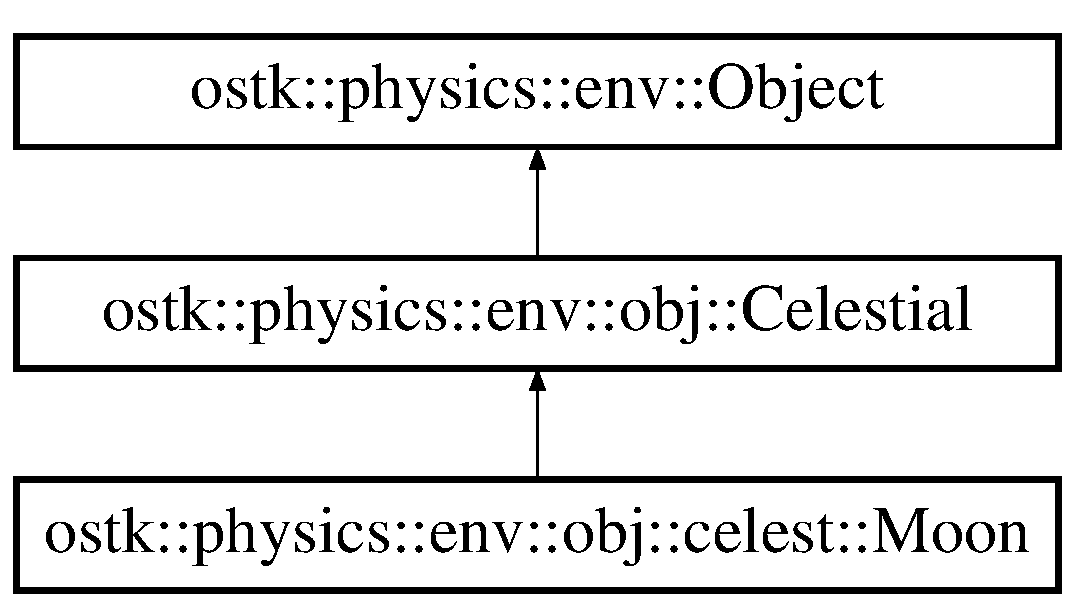
\includegraphics[height=3.000000cm]{classostk_1_1physics_1_1env_1_1obj_1_1celest_1_1_moon}
\end{center}
\end{figure}
\subsection*{Public Member Functions}
\begin{DoxyCompactItemize}
\item 
\hyperlink{classostk_1_1physics_1_1env_1_1obj_1_1celest_1_1_moon_ad8fdde672c99f064ea7ad3e6d3d8451c}{Moon} (const Shared$<$ \hyperlink{classostk_1_1physics_1_1env_1_1_ephemeris}{Ephemeris} $>$ \&an\+Ephemeris, const \hyperlink{classostk_1_1physics_1_1time_1_1_instant}{Instant} \&an\+Instant)
\item 
virtual \hyperlink{classostk_1_1physics_1_1env_1_1obj_1_1celest_1_1_moon_ad7c6677716956e7175798afa5f3bd9d4}{$\sim$\+Moon} () override
\item 
virtual \hyperlink{classostk_1_1physics_1_1env_1_1obj_1_1celest_1_1_moon}{Moon} $\ast$ \hyperlink{classostk_1_1physics_1_1env_1_1obj_1_1celest_1_1_moon_adcfeda7b73d32df67f5b38c05ca9351a}{clone} () const override
\end{DoxyCompactItemize}
\subsection*{Static Public Member Functions}
\begin{DoxyCompactItemize}
\item 
static \hyperlink{classostk_1_1physics_1_1env_1_1obj_1_1celest_1_1_moon}{Moon} \hyperlink{classostk_1_1physics_1_1env_1_1obj_1_1celest_1_1_moon_a20b7b36974130f942a113b05c4544a03}{Default} ()
\end{DoxyCompactItemize}
\subsection*{Static Public Attributes}
\begin{DoxyCompactItemize}
\item 
static \hyperlink{classostk_1_1physics_1_1units_1_1_derived}{Derived} \hyperlink{classostk_1_1physics_1_1env_1_1obj_1_1celest_1_1_moon_ad9b61b93eb0855dce7f969d68932f5c6}{Gravitational\+Parameter} = \{ 4902.\+8000e9, Derived\+::\+Unit\+::\+Gravitational\+Parameter(\+Length\+::\+Unit\+::\+Meter, Time\+::\+Unit\+::\+Second) \}
\item 
static \hyperlink{classostk_1_1physics_1_1units_1_1_length}{Length} \hyperlink{classostk_1_1physics_1_1env_1_1obj_1_1celest_1_1_moon_a955cccb5f9056296a10d4f7ea879e185}{Equatorial\+Radius} = \hyperlink{classostk_1_1physics_1_1units_1_1_length_ad227977ce00756791595796a0dd5ddd7}{Length\+::\+Meters}(1738.\+14e3)
\item 
static Real \hyperlink{classostk_1_1physics_1_1env_1_1obj_1_1celest_1_1_moon_ab66267b7075ad71aff5cbbe2469ef32c}{Flattening} = 0.\+00125
\end{DoxyCompactItemize}
\subsection*{Additional Inherited Members}


\subsection{Constructor \& Destructor Documentation}
\mbox{\Hypertarget{classostk_1_1physics_1_1env_1_1obj_1_1celest_1_1_moon_ad8fdde672c99f064ea7ad3e6d3d8451c}\label{classostk_1_1physics_1_1env_1_1obj_1_1celest_1_1_moon_ad8fdde672c99f064ea7ad3e6d3d8451c}} 
\index{ostk\+::physics\+::env\+::obj\+::celest\+::\+Moon@{ostk\+::physics\+::env\+::obj\+::celest\+::\+Moon}!Moon@{Moon}}
\index{Moon@{Moon}!ostk\+::physics\+::env\+::obj\+::celest\+::\+Moon@{ostk\+::physics\+::env\+::obj\+::celest\+::\+Moon}}
\subsubsection{\texorpdfstring{Moon()}{Moon()}}
{\footnotesize\ttfamily ostk\+::physics\+::env\+::obj\+::celest\+::\+Moon\+::\+Moon (\begin{DoxyParamCaption}\item[{const Shared$<$ \hyperlink{classostk_1_1physics_1_1env_1_1_ephemeris}{Ephemeris} $>$ \&}]{an\+Ephemeris,  }\item[{const \hyperlink{classostk_1_1physics_1_1time_1_1_instant}{Instant} \&}]{an\+Instant }\end{DoxyParamCaption})}

\mbox{\Hypertarget{classostk_1_1physics_1_1env_1_1obj_1_1celest_1_1_moon_ad7c6677716956e7175798afa5f3bd9d4}\label{classostk_1_1physics_1_1env_1_1obj_1_1celest_1_1_moon_ad7c6677716956e7175798afa5f3bd9d4}} 
\index{ostk\+::physics\+::env\+::obj\+::celest\+::\+Moon@{ostk\+::physics\+::env\+::obj\+::celest\+::\+Moon}!````~Moon@{$\sim$\+Moon}}
\index{````~Moon@{$\sim$\+Moon}!ostk\+::physics\+::env\+::obj\+::celest\+::\+Moon@{ostk\+::physics\+::env\+::obj\+::celest\+::\+Moon}}
\subsubsection{\texorpdfstring{$\sim$\+Moon()}{~Moon()}}
{\footnotesize\ttfamily ostk\+::physics\+::env\+::obj\+::celest\+::\+Moon\+::$\sim$\+Moon (\begin{DoxyParamCaption}{ }\end{DoxyParamCaption})\hspace{0.3cm}{\ttfamily [override]}, {\ttfamily [virtual]}}



\subsection{Member Function Documentation}
\mbox{\Hypertarget{classostk_1_1physics_1_1env_1_1obj_1_1celest_1_1_moon_adcfeda7b73d32df67f5b38c05ca9351a}\label{classostk_1_1physics_1_1env_1_1obj_1_1celest_1_1_moon_adcfeda7b73d32df67f5b38c05ca9351a}} 
\index{ostk\+::physics\+::env\+::obj\+::celest\+::\+Moon@{ostk\+::physics\+::env\+::obj\+::celest\+::\+Moon}!clone@{clone}}
\index{clone@{clone}!ostk\+::physics\+::env\+::obj\+::celest\+::\+Moon@{ostk\+::physics\+::env\+::obj\+::celest\+::\+Moon}}
\subsubsection{\texorpdfstring{clone()}{clone()}}
{\footnotesize\ttfamily \hyperlink{classostk_1_1physics_1_1env_1_1obj_1_1celest_1_1_moon}{Moon} $\ast$ ostk\+::physics\+::env\+::obj\+::celest\+::\+Moon\+::clone (\begin{DoxyParamCaption}{ }\end{DoxyParamCaption}) const\hspace{0.3cm}{\ttfamily [override]}, {\ttfamily [virtual]}}



Reimplemented from \hyperlink{classostk_1_1physics_1_1env_1_1obj_1_1_celestial_a87c6f3ec3c0ec9758ae52e3edc3fc5df}{ostk\+::physics\+::env\+::obj\+::\+Celestial}.

\mbox{\Hypertarget{classostk_1_1physics_1_1env_1_1obj_1_1celest_1_1_moon_a20b7b36974130f942a113b05c4544a03}\label{classostk_1_1physics_1_1env_1_1obj_1_1celest_1_1_moon_a20b7b36974130f942a113b05c4544a03}} 
\index{ostk\+::physics\+::env\+::obj\+::celest\+::\+Moon@{ostk\+::physics\+::env\+::obj\+::celest\+::\+Moon}!Default@{Default}}
\index{Default@{Default}!ostk\+::physics\+::env\+::obj\+::celest\+::\+Moon@{ostk\+::physics\+::env\+::obj\+::celest\+::\+Moon}}
\subsubsection{\texorpdfstring{Default()}{Default()}}
{\footnotesize\ttfamily \hyperlink{classostk_1_1physics_1_1env_1_1obj_1_1celest_1_1_moon}{Moon} ostk\+::physics\+::env\+::obj\+::celest\+::\+Moon\+::\+Default (\begin{DoxyParamCaption}{ }\end{DoxyParamCaption})\hspace{0.3cm}{\ttfamily [static]}}



\subsection{Member Data Documentation}
\mbox{\Hypertarget{classostk_1_1physics_1_1env_1_1obj_1_1celest_1_1_moon_a955cccb5f9056296a10d4f7ea879e185}\label{classostk_1_1physics_1_1env_1_1obj_1_1celest_1_1_moon_a955cccb5f9056296a10d4f7ea879e185}} 
\index{ostk\+::physics\+::env\+::obj\+::celest\+::\+Moon@{ostk\+::physics\+::env\+::obj\+::celest\+::\+Moon}!Equatorial\+Radius@{Equatorial\+Radius}}
\index{Equatorial\+Radius@{Equatorial\+Radius}!ostk\+::physics\+::env\+::obj\+::celest\+::\+Moon@{ostk\+::physics\+::env\+::obj\+::celest\+::\+Moon}}
\subsubsection{\texorpdfstring{Equatorial\+Radius}{EquatorialRadius}}
{\footnotesize\ttfamily \hyperlink{classostk_1_1physics_1_1units_1_1_length}{Length} ostk\+::physics\+::env\+::obj\+::celest\+::\+Moon\+::\+Equatorial\+Radius = \hyperlink{classostk_1_1physics_1_1units_1_1_length_ad227977ce00756791595796a0dd5ddd7}{Length\+::\+Meters}(1738.\+14e3)\hspace{0.3cm}{\ttfamily [static]}}

\mbox{\Hypertarget{classostk_1_1physics_1_1env_1_1obj_1_1celest_1_1_moon_ab66267b7075ad71aff5cbbe2469ef32c}\label{classostk_1_1physics_1_1env_1_1obj_1_1celest_1_1_moon_ab66267b7075ad71aff5cbbe2469ef32c}} 
\index{ostk\+::physics\+::env\+::obj\+::celest\+::\+Moon@{ostk\+::physics\+::env\+::obj\+::celest\+::\+Moon}!Flattening@{Flattening}}
\index{Flattening@{Flattening}!ostk\+::physics\+::env\+::obj\+::celest\+::\+Moon@{ostk\+::physics\+::env\+::obj\+::celest\+::\+Moon}}
\subsubsection{\texorpdfstring{Flattening}{Flattening}}
{\footnotesize\ttfamily Real ostk\+::physics\+::env\+::obj\+::celest\+::\+Moon\+::\+Flattening = 0.\+00125\hspace{0.3cm}{\ttfamily [static]}}

\mbox{\Hypertarget{classostk_1_1physics_1_1env_1_1obj_1_1celest_1_1_moon_ad9b61b93eb0855dce7f969d68932f5c6}\label{classostk_1_1physics_1_1env_1_1obj_1_1celest_1_1_moon_ad9b61b93eb0855dce7f969d68932f5c6}} 
\index{ostk\+::physics\+::env\+::obj\+::celest\+::\+Moon@{ostk\+::physics\+::env\+::obj\+::celest\+::\+Moon}!Gravitational\+Parameter@{Gravitational\+Parameter}}
\index{Gravitational\+Parameter@{Gravitational\+Parameter}!ostk\+::physics\+::env\+::obj\+::celest\+::\+Moon@{ostk\+::physics\+::env\+::obj\+::celest\+::\+Moon}}
\subsubsection{\texorpdfstring{Gravitational\+Parameter}{GravitationalParameter}}
{\footnotesize\ttfamily \hyperlink{classostk_1_1physics_1_1units_1_1_derived}{Derived} ostk\+::physics\+::env\+::obj\+::celest\+::\+Moon\+::\+Gravitational\+Parameter = \{ 4902.\+8000e9, Derived\+::\+Unit\+::\+Gravitational\+Parameter(\+Length\+::\+Unit\+::\+Meter, Time\+::\+Unit\+::\+Second) \}\hspace{0.3cm}{\ttfamily [static]}}



The documentation for this class was generated from the following files\+:\begin{DoxyCompactItemize}
\item 
include/\+Open\+Space\+Toolkit/\+Physics/\+Environment/\+Objects/\+Celestial\+Bodies/\hyperlink{_moon_8hpp}{Moon.\+hpp}\item 
src/\+Open\+Space\+Toolkit/\+Physics/\+Environment/\+Objects/\+Celestial\+Bodies/\hyperlink{_moon_8cpp}{Moon.\+cpp}\end{DoxyCompactItemize}

\hypertarget{classostk_1_1physics_1_1env_1_1_object}{}\section{ostk\+:\+:physics\+:\+:env\+:\+:Object Class Reference}
\label{classostk_1_1physics_1_1env_1_1_object}\index{ostk\+::physics\+::env\+::\+Object@{ostk\+::physics\+::env\+::\+Object}}


{\ttfamily \#include $<$Object.\+hpp$>$}

Inheritance diagram for ostk\+:\+:physics\+:\+:env\+:\+:Object\+:\begin{figure}[H]
\begin{center}
\leavevmode
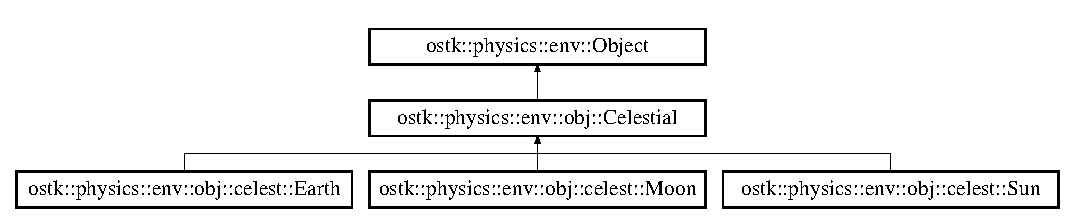
\includegraphics[height=2.568807cm]{classostk_1_1physics_1_1env_1_1_object}
\end{center}
\end{figure}
\subsection*{Public Types}
\begin{DoxyCompactItemize}
\item 
typedef \hyperlink{classostk_1_1physics_1_1env_1_1object_1_1_geometry}{object\+::\+Geometry} \hyperlink{classostk_1_1physics_1_1env_1_1_object_a66e44a65aefb23a184a6de531e96935d}{Geometry}
\end{DoxyCompactItemize}
\subsection*{Public Member Functions}
\begin{DoxyCompactItemize}
\item 
\hyperlink{classostk_1_1physics_1_1env_1_1_object_acd023212c67c893a753f1f3e2cf5c745}{Object} (const String \&a\+Name, const \hyperlink{classostk_1_1physics_1_1time_1_1_instant}{Instant} \&an\+Instant)
\item 
\hyperlink{classostk_1_1physics_1_1env_1_1_object_a8b314016640cee6729de6ae6364ba51f}{Object} (const String \&a\+Name, const \hyperlink{classostk_1_1physics_1_1time_1_1_instant}{Instant} \&an\+Instant, const \hyperlink{classostk_1_1physics_1_1env_1_1_object_a66e44a65aefb23a184a6de531e96935d}{Object\+::\+Geometry} \&a\+Geometry)
\item 
\hyperlink{classostk_1_1physics_1_1env_1_1_object_abddb73324d38f53b395ebee283e78ce1}{Object} (const \hyperlink{classostk_1_1physics_1_1env_1_1_object}{Object} \&an\+Object)
\item 
virtual \hyperlink{classostk_1_1physics_1_1env_1_1_object_a317cd99f9e64b168ca28a7e1dbcf1cbc}{$\sim$\+Object} ()=0
\item 
virtual \hyperlink{classostk_1_1physics_1_1env_1_1_object}{Object} $\ast$ \hyperlink{classostk_1_1physics_1_1env_1_1_object_a8e45ece3cf6d7be05a984a8857b7ecd3}{clone} () const =0
\item 
\hyperlink{classostk_1_1physics_1_1env_1_1_object}{Object} \& \hyperlink{classostk_1_1physics_1_1env_1_1_object_aebe1f6eca2d149968f496577fd291296}{operator=} (const \hyperlink{classostk_1_1physics_1_1env_1_1_object}{Object} \&an\+Object)
\item 
virtual bool \hyperlink{classostk_1_1physics_1_1env_1_1_object_aaa5131bafbaf86fde7f649e88343a901}{is\+Defined} () const
\item 
const String \& \hyperlink{classostk_1_1physics_1_1env_1_1_object_aea899eb9d809f8b344127ceb5c1056c4}{access\+Name} () const
\item 
const \hyperlink{classostk_1_1physics_1_1time_1_1_instant}{Instant} \& \hyperlink{classostk_1_1physics_1_1env_1_1_object_ae0a8b4a06e5dce1c295911f0f81f0ac0}{access\+Instant} () const
\item 
virtual Shared$<$ const \hyperlink{classostk_1_1physics_1_1coord_1_1_frame}{Frame} $>$ \hyperlink{classostk_1_1physics_1_1env_1_1_object_aca93358323c3eb3e4dabf07c33187f14}{access\+Frame} () const =0
\item 
const \hyperlink{classostk_1_1physics_1_1env_1_1_object_a66e44a65aefb23a184a6de531e96935d}{Object\+::\+Geometry} \& \hyperlink{classostk_1_1physics_1_1env_1_1_object_af5556cdc8db2a35e8549b79d481ceada}{access\+Geometry} () const
\item 
String \hyperlink{classostk_1_1physics_1_1env_1_1_object_a4157537667421ed215929113222ef909}{get\+Name} () const
\item 
\hyperlink{classostk_1_1physics_1_1time_1_1_instant}{Instant} \hyperlink{classostk_1_1physics_1_1env_1_1_object_ac0b6d3717624300bb9f5576996c00077}{get\+Instant} () const
\item 
\hyperlink{classostk_1_1physics_1_1env_1_1_object_a66e44a65aefb23a184a6de531e96935d}{Object\+::\+Geometry} \hyperlink{classostk_1_1physics_1_1env_1_1_object_aa74070ed996907de5a2821233d1aa555}{get\+Geometry} () const
\item 
virtual \hyperlink{classostk_1_1physics_1_1coord_1_1_position}{Position} \hyperlink{classostk_1_1physics_1_1env_1_1_object_a990c33e0cc9e9421488f9fc4cbbf3f21}{get\+Position\+In} (const Shared$<$ const \hyperlink{classostk_1_1physics_1_1coord_1_1_frame}{Frame} $>$ \&a\+Frame\+S\+Ptr) const =0
\item 
virtual \hyperlink{classostk_1_1physics_1_1coord_1_1_velocity}{Velocity} \hyperlink{classostk_1_1physics_1_1env_1_1_object_a216c8d5e44451fd664e0c7eb3b4934b6}{get\+Velocity\+In} (const Shared$<$ const \hyperlink{classostk_1_1physics_1_1coord_1_1_frame}{Frame} $>$ \&a\+Frame\+S\+Ptr) const =0
\item 
virtual \hyperlink{classostk_1_1physics_1_1coord_1_1_transform}{Transform} \hyperlink{classostk_1_1physics_1_1env_1_1_object_a720f81e696c3f4f81de8e7ae787fdf10}{get\+Transform\+To} (const Shared$<$ const \hyperlink{classostk_1_1physics_1_1coord_1_1_frame}{Frame} $>$ \&a\+Frame\+S\+Ptr) const =0
\item 
virtual \hyperlink{classostk_1_1physics_1_1coord_1_1_axes}{Axes} \hyperlink{classostk_1_1physics_1_1env_1_1_object_a706d29c77ce311a3abcf2a6060515711}{get\+Axes\+In} (const Shared$<$ const \hyperlink{classostk_1_1physics_1_1coord_1_1_frame}{Frame} $>$ \&a\+Frame\+S\+Ptr) const =0
\item 
\hyperlink{classostk_1_1physics_1_1env_1_1_object_a66e44a65aefb23a184a6de531e96935d}{Object\+::\+Geometry} \hyperlink{classostk_1_1physics_1_1env_1_1_object_adb5784e72236cf93239d8a726fae45ac}{get\+Geometry\+In} (const Shared$<$ const \hyperlink{classostk_1_1physics_1_1coord_1_1_frame}{Frame} $>$ \&a\+Frame\+S\+Ptr) const
\item 
void \hyperlink{classostk_1_1physics_1_1env_1_1_object_a1cfbdcd0259692801469fbefee7790a6}{set\+Instant} (const \hyperlink{classostk_1_1physics_1_1time_1_1_instant}{Instant} \&an\+Instant)
\end{DoxyCompactItemize}
\subsection*{Friends}
\begin{DoxyCompactItemize}
\item 
std\+::ostream \& \hyperlink{classostk_1_1physics_1_1env_1_1_object_a418df9bf4a73078f3d494edef1743f8d}{operator$<$$<$} (std\+::ostream \&an\+Output\+Stream, const \hyperlink{classostk_1_1physics_1_1env_1_1_object}{Object} \&an\+Object)
\end{DoxyCompactItemize}


\subsection{Member Typedef Documentation}
\mbox{\Hypertarget{classostk_1_1physics_1_1env_1_1_object_a66e44a65aefb23a184a6de531e96935d}\label{classostk_1_1physics_1_1env_1_1_object_a66e44a65aefb23a184a6de531e96935d}} 
\index{ostk\+::physics\+::env\+::\+Object@{ostk\+::physics\+::env\+::\+Object}!Geometry@{Geometry}}
\index{Geometry@{Geometry}!ostk\+::physics\+::env\+::\+Object@{ostk\+::physics\+::env\+::\+Object}}
\subsubsection{\texorpdfstring{Geometry}{Geometry}}
{\footnotesize\ttfamily typedef \hyperlink{classostk_1_1physics_1_1env_1_1object_1_1_geometry}{object\+::\+Geometry} \hyperlink{classostk_1_1physics_1_1env_1_1_object_a66e44a65aefb23a184a6de531e96935d}{ostk\+::physics\+::env\+::\+Object\+::\+Geometry}}



\subsection{Constructor \& Destructor Documentation}
\mbox{\Hypertarget{classostk_1_1physics_1_1env_1_1_object_acd023212c67c893a753f1f3e2cf5c745}\label{classostk_1_1physics_1_1env_1_1_object_acd023212c67c893a753f1f3e2cf5c745}} 
\index{ostk\+::physics\+::env\+::\+Object@{ostk\+::physics\+::env\+::\+Object}!Object@{Object}}
\index{Object@{Object}!ostk\+::physics\+::env\+::\+Object@{ostk\+::physics\+::env\+::\+Object}}
\subsubsection{\texorpdfstring{Object()}{Object()}\hspace{0.1cm}{\footnotesize\ttfamily [1/3]}}
{\footnotesize\ttfamily ostk\+::physics\+::env\+::\+Object\+::\+Object (\begin{DoxyParamCaption}\item[{const String \&}]{a\+Name,  }\item[{const \hyperlink{classostk_1_1physics_1_1time_1_1_instant}{Instant} \&}]{an\+Instant }\end{DoxyParamCaption})}

\mbox{\Hypertarget{classostk_1_1physics_1_1env_1_1_object_a8b314016640cee6729de6ae6364ba51f}\label{classostk_1_1physics_1_1env_1_1_object_a8b314016640cee6729de6ae6364ba51f}} 
\index{ostk\+::physics\+::env\+::\+Object@{ostk\+::physics\+::env\+::\+Object}!Object@{Object}}
\index{Object@{Object}!ostk\+::physics\+::env\+::\+Object@{ostk\+::physics\+::env\+::\+Object}}
\subsubsection{\texorpdfstring{Object()}{Object()}\hspace{0.1cm}{\footnotesize\ttfamily [2/3]}}
{\footnotesize\ttfamily ostk\+::physics\+::env\+::\+Object\+::\+Object (\begin{DoxyParamCaption}\item[{const String \&}]{a\+Name,  }\item[{const \hyperlink{classostk_1_1physics_1_1time_1_1_instant}{Instant} \&}]{an\+Instant,  }\item[{const \hyperlink{classostk_1_1physics_1_1env_1_1_object_a66e44a65aefb23a184a6de531e96935d}{Object\+::\+Geometry} \&}]{a\+Geometry }\end{DoxyParamCaption})}

\mbox{\Hypertarget{classostk_1_1physics_1_1env_1_1_object_abddb73324d38f53b395ebee283e78ce1}\label{classostk_1_1physics_1_1env_1_1_object_abddb73324d38f53b395ebee283e78ce1}} 
\index{ostk\+::physics\+::env\+::\+Object@{ostk\+::physics\+::env\+::\+Object}!Object@{Object}}
\index{Object@{Object}!ostk\+::physics\+::env\+::\+Object@{ostk\+::physics\+::env\+::\+Object}}
\subsubsection{\texorpdfstring{Object()}{Object()}\hspace{0.1cm}{\footnotesize\ttfamily [3/3]}}
{\footnotesize\ttfamily ostk\+::physics\+::env\+::\+Object\+::\+Object (\begin{DoxyParamCaption}\item[{const \hyperlink{classostk_1_1physics_1_1env_1_1_object}{Object} \&}]{an\+Object }\end{DoxyParamCaption})}

\mbox{\Hypertarget{classostk_1_1physics_1_1env_1_1_object_a317cd99f9e64b168ca28a7e1dbcf1cbc}\label{classostk_1_1physics_1_1env_1_1_object_a317cd99f9e64b168ca28a7e1dbcf1cbc}} 
\index{ostk\+::physics\+::env\+::\+Object@{ostk\+::physics\+::env\+::\+Object}!````~Object@{$\sim$\+Object}}
\index{````~Object@{$\sim$\+Object}!ostk\+::physics\+::env\+::\+Object@{ostk\+::physics\+::env\+::\+Object}}
\subsubsection{\texorpdfstring{$\sim$\+Object()}{~Object()}}
{\footnotesize\ttfamily ostk\+::physics\+::env\+::\+Object\+::$\sim$\+Object (\begin{DoxyParamCaption}{ }\end{DoxyParamCaption})\hspace{0.3cm}{\ttfamily [pure virtual]}}



\subsection{Member Function Documentation}
\mbox{\Hypertarget{classostk_1_1physics_1_1env_1_1_object_aca93358323c3eb3e4dabf07c33187f14}\label{classostk_1_1physics_1_1env_1_1_object_aca93358323c3eb3e4dabf07c33187f14}} 
\index{ostk\+::physics\+::env\+::\+Object@{ostk\+::physics\+::env\+::\+Object}!access\+Frame@{access\+Frame}}
\index{access\+Frame@{access\+Frame}!ostk\+::physics\+::env\+::\+Object@{ostk\+::physics\+::env\+::\+Object}}
\subsubsection{\texorpdfstring{access\+Frame()}{accessFrame()}}
{\footnotesize\ttfamily virtual Shared$<$const \hyperlink{classostk_1_1physics_1_1coord_1_1_frame}{Frame}$>$ ostk\+::physics\+::env\+::\+Object\+::access\+Frame (\begin{DoxyParamCaption}{ }\end{DoxyParamCaption}) const\hspace{0.3cm}{\ttfamily [pure virtual]}}



Implemented in \hyperlink{classostk_1_1physics_1_1env_1_1obj_1_1_celestial_a0140fc682a707ec2dc715828e532db79}{ostk\+::physics\+::env\+::obj\+::\+Celestial}.

\mbox{\Hypertarget{classostk_1_1physics_1_1env_1_1_object_af5556cdc8db2a35e8549b79d481ceada}\label{classostk_1_1physics_1_1env_1_1_object_af5556cdc8db2a35e8549b79d481ceada}} 
\index{ostk\+::physics\+::env\+::\+Object@{ostk\+::physics\+::env\+::\+Object}!access\+Geometry@{access\+Geometry}}
\index{access\+Geometry@{access\+Geometry}!ostk\+::physics\+::env\+::\+Object@{ostk\+::physics\+::env\+::\+Object}}
\subsubsection{\texorpdfstring{access\+Geometry()}{accessGeometry()}}
{\footnotesize\ttfamily const \hyperlink{classostk_1_1physics_1_1env_1_1_object_a66e44a65aefb23a184a6de531e96935d}{Object\+::\+Geometry} \& ostk\+::physics\+::env\+::\+Object\+::access\+Geometry (\begin{DoxyParamCaption}{ }\end{DoxyParamCaption}) const}

\mbox{\Hypertarget{classostk_1_1physics_1_1env_1_1_object_ae0a8b4a06e5dce1c295911f0f81f0ac0}\label{classostk_1_1physics_1_1env_1_1_object_ae0a8b4a06e5dce1c295911f0f81f0ac0}} 
\index{ostk\+::physics\+::env\+::\+Object@{ostk\+::physics\+::env\+::\+Object}!access\+Instant@{access\+Instant}}
\index{access\+Instant@{access\+Instant}!ostk\+::physics\+::env\+::\+Object@{ostk\+::physics\+::env\+::\+Object}}
\subsubsection{\texorpdfstring{access\+Instant()}{accessInstant()}}
{\footnotesize\ttfamily const \hyperlink{classostk_1_1physics_1_1time_1_1_instant}{Instant} \& ostk\+::physics\+::env\+::\+Object\+::access\+Instant (\begin{DoxyParamCaption}{ }\end{DoxyParamCaption}) const}

\mbox{\Hypertarget{classostk_1_1physics_1_1env_1_1_object_aea899eb9d809f8b344127ceb5c1056c4}\label{classostk_1_1physics_1_1env_1_1_object_aea899eb9d809f8b344127ceb5c1056c4}} 
\index{ostk\+::physics\+::env\+::\+Object@{ostk\+::physics\+::env\+::\+Object}!access\+Name@{access\+Name}}
\index{access\+Name@{access\+Name}!ostk\+::physics\+::env\+::\+Object@{ostk\+::physics\+::env\+::\+Object}}
\subsubsection{\texorpdfstring{access\+Name()}{accessName()}}
{\footnotesize\ttfamily const String \& ostk\+::physics\+::env\+::\+Object\+::access\+Name (\begin{DoxyParamCaption}{ }\end{DoxyParamCaption}) const}

\mbox{\Hypertarget{classostk_1_1physics_1_1env_1_1_object_a8e45ece3cf6d7be05a984a8857b7ecd3}\label{classostk_1_1physics_1_1env_1_1_object_a8e45ece3cf6d7be05a984a8857b7ecd3}} 
\index{ostk\+::physics\+::env\+::\+Object@{ostk\+::physics\+::env\+::\+Object}!clone@{clone}}
\index{clone@{clone}!ostk\+::physics\+::env\+::\+Object@{ostk\+::physics\+::env\+::\+Object}}
\subsubsection{\texorpdfstring{clone()}{clone()}}
{\footnotesize\ttfamily virtual \hyperlink{classostk_1_1physics_1_1env_1_1_object}{Object}$\ast$ ostk\+::physics\+::env\+::\+Object\+::clone (\begin{DoxyParamCaption}{ }\end{DoxyParamCaption}) const\hspace{0.3cm}{\ttfamily [pure virtual]}}



Implemented in \hyperlink{classostk_1_1physics_1_1env_1_1obj_1_1_celestial_a87c6f3ec3c0ec9758ae52e3edc3fc5df}{ostk\+::physics\+::env\+::obj\+::\+Celestial}, \hyperlink{classostk_1_1physics_1_1env_1_1obj_1_1celest_1_1_earth_ae86664b9d6fc870baa1dac5c3219f784}{ostk\+::physics\+::env\+::obj\+::celest\+::\+Earth}, \hyperlink{classostk_1_1physics_1_1env_1_1obj_1_1celest_1_1_moon_adcfeda7b73d32df67f5b38c05ca9351a}{ostk\+::physics\+::env\+::obj\+::celest\+::\+Moon}, and \hyperlink{classostk_1_1physics_1_1env_1_1obj_1_1celest_1_1_sun_a57fd7c3c48115f77e2d3d331ef0e8e0a}{ostk\+::physics\+::env\+::obj\+::celest\+::\+Sun}.

\mbox{\Hypertarget{classostk_1_1physics_1_1env_1_1_object_a706d29c77ce311a3abcf2a6060515711}\label{classostk_1_1physics_1_1env_1_1_object_a706d29c77ce311a3abcf2a6060515711}} 
\index{ostk\+::physics\+::env\+::\+Object@{ostk\+::physics\+::env\+::\+Object}!get\+Axes\+In@{get\+Axes\+In}}
\index{get\+Axes\+In@{get\+Axes\+In}!ostk\+::physics\+::env\+::\+Object@{ostk\+::physics\+::env\+::\+Object}}
\subsubsection{\texorpdfstring{get\+Axes\+In()}{getAxesIn()}}
{\footnotesize\ttfamily virtual \hyperlink{classostk_1_1physics_1_1coord_1_1_axes}{Axes} ostk\+::physics\+::env\+::\+Object\+::get\+Axes\+In (\begin{DoxyParamCaption}\item[{const Shared$<$ const \hyperlink{classostk_1_1physics_1_1coord_1_1_frame}{Frame} $>$ \&}]{a\+Frame\+S\+Ptr }\end{DoxyParamCaption}) const\hspace{0.3cm}{\ttfamily [pure virtual]}}



Implemented in \hyperlink{classostk_1_1physics_1_1env_1_1obj_1_1_celestial_a52b8cd88b947ca97f94981e5d3e10677}{ostk\+::physics\+::env\+::obj\+::\+Celestial}.

\mbox{\Hypertarget{classostk_1_1physics_1_1env_1_1_object_aa74070ed996907de5a2821233d1aa555}\label{classostk_1_1physics_1_1env_1_1_object_aa74070ed996907de5a2821233d1aa555}} 
\index{ostk\+::physics\+::env\+::\+Object@{ostk\+::physics\+::env\+::\+Object}!get\+Geometry@{get\+Geometry}}
\index{get\+Geometry@{get\+Geometry}!ostk\+::physics\+::env\+::\+Object@{ostk\+::physics\+::env\+::\+Object}}
\subsubsection{\texorpdfstring{get\+Geometry()}{getGeometry()}}
{\footnotesize\ttfamily \hyperlink{classostk_1_1physics_1_1env_1_1_object_a66e44a65aefb23a184a6de531e96935d}{Object\+::\+Geometry} ostk\+::physics\+::env\+::\+Object\+::get\+Geometry (\begin{DoxyParamCaption}{ }\end{DoxyParamCaption}) const}

\mbox{\Hypertarget{classostk_1_1physics_1_1env_1_1_object_adb5784e72236cf93239d8a726fae45ac}\label{classostk_1_1physics_1_1env_1_1_object_adb5784e72236cf93239d8a726fae45ac}} 
\index{ostk\+::physics\+::env\+::\+Object@{ostk\+::physics\+::env\+::\+Object}!get\+Geometry\+In@{get\+Geometry\+In}}
\index{get\+Geometry\+In@{get\+Geometry\+In}!ostk\+::physics\+::env\+::\+Object@{ostk\+::physics\+::env\+::\+Object}}
\subsubsection{\texorpdfstring{get\+Geometry\+In()}{getGeometryIn()}}
{\footnotesize\ttfamily \hyperlink{classostk_1_1physics_1_1env_1_1_object_a66e44a65aefb23a184a6de531e96935d}{Object\+::\+Geometry} ostk\+::physics\+::env\+::\+Object\+::get\+Geometry\+In (\begin{DoxyParamCaption}\item[{const Shared$<$ const \hyperlink{classostk_1_1physics_1_1coord_1_1_frame}{Frame} $>$ \&}]{a\+Frame\+S\+Ptr }\end{DoxyParamCaption}) const}

\mbox{\Hypertarget{classostk_1_1physics_1_1env_1_1_object_ac0b6d3717624300bb9f5576996c00077}\label{classostk_1_1physics_1_1env_1_1_object_ac0b6d3717624300bb9f5576996c00077}} 
\index{ostk\+::physics\+::env\+::\+Object@{ostk\+::physics\+::env\+::\+Object}!get\+Instant@{get\+Instant}}
\index{get\+Instant@{get\+Instant}!ostk\+::physics\+::env\+::\+Object@{ostk\+::physics\+::env\+::\+Object}}
\subsubsection{\texorpdfstring{get\+Instant()}{getInstant()}}
{\footnotesize\ttfamily \hyperlink{classostk_1_1physics_1_1time_1_1_instant}{Instant} ostk\+::physics\+::env\+::\+Object\+::get\+Instant (\begin{DoxyParamCaption}{ }\end{DoxyParamCaption}) const}

\mbox{\Hypertarget{classostk_1_1physics_1_1env_1_1_object_a4157537667421ed215929113222ef909}\label{classostk_1_1physics_1_1env_1_1_object_a4157537667421ed215929113222ef909}} 
\index{ostk\+::physics\+::env\+::\+Object@{ostk\+::physics\+::env\+::\+Object}!get\+Name@{get\+Name}}
\index{get\+Name@{get\+Name}!ostk\+::physics\+::env\+::\+Object@{ostk\+::physics\+::env\+::\+Object}}
\subsubsection{\texorpdfstring{get\+Name()}{getName()}}
{\footnotesize\ttfamily String ostk\+::physics\+::env\+::\+Object\+::get\+Name (\begin{DoxyParamCaption}{ }\end{DoxyParamCaption}) const}

\mbox{\Hypertarget{classostk_1_1physics_1_1env_1_1_object_a990c33e0cc9e9421488f9fc4cbbf3f21}\label{classostk_1_1physics_1_1env_1_1_object_a990c33e0cc9e9421488f9fc4cbbf3f21}} 
\index{ostk\+::physics\+::env\+::\+Object@{ostk\+::physics\+::env\+::\+Object}!get\+Position\+In@{get\+Position\+In}}
\index{get\+Position\+In@{get\+Position\+In}!ostk\+::physics\+::env\+::\+Object@{ostk\+::physics\+::env\+::\+Object}}
\subsubsection{\texorpdfstring{get\+Position\+In()}{getPositionIn()}}
{\footnotesize\ttfamily virtual \hyperlink{classostk_1_1physics_1_1coord_1_1_position}{Position} ostk\+::physics\+::env\+::\+Object\+::get\+Position\+In (\begin{DoxyParamCaption}\item[{const Shared$<$ const \hyperlink{classostk_1_1physics_1_1coord_1_1_frame}{Frame} $>$ \&}]{a\+Frame\+S\+Ptr }\end{DoxyParamCaption}) const\hspace{0.3cm}{\ttfamily [pure virtual]}}



Implemented in \hyperlink{classostk_1_1physics_1_1env_1_1obj_1_1_celestial_af38fd0017fe14cfb6103684fcb1d3ee9}{ostk\+::physics\+::env\+::obj\+::\+Celestial}.

\mbox{\Hypertarget{classostk_1_1physics_1_1env_1_1_object_a720f81e696c3f4f81de8e7ae787fdf10}\label{classostk_1_1physics_1_1env_1_1_object_a720f81e696c3f4f81de8e7ae787fdf10}} 
\index{ostk\+::physics\+::env\+::\+Object@{ostk\+::physics\+::env\+::\+Object}!get\+Transform\+To@{get\+Transform\+To}}
\index{get\+Transform\+To@{get\+Transform\+To}!ostk\+::physics\+::env\+::\+Object@{ostk\+::physics\+::env\+::\+Object}}
\subsubsection{\texorpdfstring{get\+Transform\+To()}{getTransformTo()}}
{\footnotesize\ttfamily virtual \hyperlink{classostk_1_1physics_1_1coord_1_1_transform}{Transform} ostk\+::physics\+::env\+::\+Object\+::get\+Transform\+To (\begin{DoxyParamCaption}\item[{const Shared$<$ const \hyperlink{classostk_1_1physics_1_1coord_1_1_frame}{Frame} $>$ \&}]{a\+Frame\+S\+Ptr }\end{DoxyParamCaption}) const\hspace{0.3cm}{\ttfamily [pure virtual]}}



Implemented in \hyperlink{classostk_1_1physics_1_1env_1_1obj_1_1_celestial_a8fa63af32cf8785ff6d3762d6f8dcd86}{ostk\+::physics\+::env\+::obj\+::\+Celestial}.

\mbox{\Hypertarget{classostk_1_1physics_1_1env_1_1_object_a216c8d5e44451fd664e0c7eb3b4934b6}\label{classostk_1_1physics_1_1env_1_1_object_a216c8d5e44451fd664e0c7eb3b4934b6}} 
\index{ostk\+::physics\+::env\+::\+Object@{ostk\+::physics\+::env\+::\+Object}!get\+Velocity\+In@{get\+Velocity\+In}}
\index{get\+Velocity\+In@{get\+Velocity\+In}!ostk\+::physics\+::env\+::\+Object@{ostk\+::physics\+::env\+::\+Object}}
\subsubsection{\texorpdfstring{get\+Velocity\+In()}{getVelocityIn()}}
{\footnotesize\ttfamily virtual \hyperlink{classostk_1_1physics_1_1coord_1_1_velocity}{Velocity} ostk\+::physics\+::env\+::\+Object\+::get\+Velocity\+In (\begin{DoxyParamCaption}\item[{const Shared$<$ const \hyperlink{classostk_1_1physics_1_1coord_1_1_frame}{Frame} $>$ \&}]{a\+Frame\+S\+Ptr }\end{DoxyParamCaption}) const\hspace{0.3cm}{\ttfamily [pure virtual]}}



Implemented in \hyperlink{classostk_1_1physics_1_1env_1_1obj_1_1_celestial_a748a113566d79c463e84bf62f05af83a}{ostk\+::physics\+::env\+::obj\+::\+Celestial}.

\mbox{\Hypertarget{classostk_1_1physics_1_1env_1_1_object_aaa5131bafbaf86fde7f649e88343a901}\label{classostk_1_1physics_1_1env_1_1_object_aaa5131bafbaf86fde7f649e88343a901}} 
\index{ostk\+::physics\+::env\+::\+Object@{ostk\+::physics\+::env\+::\+Object}!is\+Defined@{is\+Defined}}
\index{is\+Defined@{is\+Defined}!ostk\+::physics\+::env\+::\+Object@{ostk\+::physics\+::env\+::\+Object}}
\subsubsection{\texorpdfstring{is\+Defined()}{isDefined()}}
{\footnotesize\ttfamily bool ostk\+::physics\+::env\+::\+Object\+::is\+Defined (\begin{DoxyParamCaption}{ }\end{DoxyParamCaption}) const\hspace{0.3cm}{\ttfamily [virtual]}}



Reimplemented in \hyperlink{classostk_1_1physics_1_1env_1_1obj_1_1_celestial_a611b8fe6fcd3787bbf9981ad99dfe471}{ostk\+::physics\+::env\+::obj\+::\+Celestial}.

\mbox{\Hypertarget{classostk_1_1physics_1_1env_1_1_object_aebe1f6eca2d149968f496577fd291296}\label{classostk_1_1physics_1_1env_1_1_object_aebe1f6eca2d149968f496577fd291296}} 
\index{ostk\+::physics\+::env\+::\+Object@{ostk\+::physics\+::env\+::\+Object}!operator=@{operator=}}
\index{operator=@{operator=}!ostk\+::physics\+::env\+::\+Object@{ostk\+::physics\+::env\+::\+Object}}
\subsubsection{\texorpdfstring{operator=()}{operator=()}}
{\footnotesize\ttfamily \hyperlink{classostk_1_1physics_1_1env_1_1_object}{Object} \& ostk\+::physics\+::env\+::\+Object\+::operator= (\begin{DoxyParamCaption}\item[{const \hyperlink{classostk_1_1physics_1_1env_1_1_object}{Object} \&}]{an\+Object }\end{DoxyParamCaption})}

\mbox{\Hypertarget{classostk_1_1physics_1_1env_1_1_object_a1cfbdcd0259692801469fbefee7790a6}\label{classostk_1_1physics_1_1env_1_1_object_a1cfbdcd0259692801469fbefee7790a6}} 
\index{ostk\+::physics\+::env\+::\+Object@{ostk\+::physics\+::env\+::\+Object}!set\+Instant@{set\+Instant}}
\index{set\+Instant@{set\+Instant}!ostk\+::physics\+::env\+::\+Object@{ostk\+::physics\+::env\+::\+Object}}
\subsubsection{\texorpdfstring{set\+Instant()}{setInstant()}}
{\footnotesize\ttfamily void ostk\+::physics\+::env\+::\+Object\+::set\+Instant (\begin{DoxyParamCaption}\item[{const \hyperlink{classostk_1_1physics_1_1time_1_1_instant}{Instant} \&}]{an\+Instant }\end{DoxyParamCaption})}



\subsection{Friends And Related Function Documentation}
\mbox{\Hypertarget{classostk_1_1physics_1_1env_1_1_object_a418df9bf4a73078f3d494edef1743f8d}\label{classostk_1_1physics_1_1env_1_1_object_a418df9bf4a73078f3d494edef1743f8d}} 
\index{ostk\+::physics\+::env\+::\+Object@{ostk\+::physics\+::env\+::\+Object}!operator$<$$<$@{operator$<$$<$}}
\index{operator$<$$<$@{operator$<$$<$}!ostk\+::physics\+::env\+::\+Object@{ostk\+::physics\+::env\+::\+Object}}
\subsubsection{\texorpdfstring{operator$<$$<$}{operator<<}}
{\footnotesize\ttfamily std\+::ostream\& operator$<$$<$ (\begin{DoxyParamCaption}\item[{std\+::ostream \&}]{an\+Output\+Stream,  }\item[{const \hyperlink{classostk_1_1physics_1_1env_1_1_object}{Object} \&}]{an\+Object }\end{DoxyParamCaption})\hspace{0.3cm}{\ttfamily [friend]}}



The documentation for this class was generated from the following files\+:\begin{DoxyCompactItemize}
\item 
include/\+Open\+Space\+Toolkit/\+Physics/\+Environment/\hyperlink{_object_8hpp}{Object.\+hpp}\item 
src/\+Open\+Space\+Toolkit/\+Physics/\+Environment/\hyperlink{_object_8cpp}{Object.\+cpp}\end{DoxyCompactItemize}

\hypertarget{structostk_1_1physics_1_1coord_1_1frame_1_1provider_1_1iers_1_1_bulletin_a_1_1_observation}{}\section{ostk\+:\+:physics\+:\+:coord\+:\+:frame\+:\+:provider\+:\+:iers\+:\+:BulletinA\+:\+:Observation Struct Reference}
\label{structostk_1_1physics_1_1coord_1_1frame_1_1provider_1_1iers_1_1_bulletin_a_1_1_observation}\index{ostk\+::physics\+::coord\+::frame\+::provider\+::iers\+::\+Bulletin\+A\+::\+Observation@{ostk\+::physics\+::coord\+::frame\+::provider\+::iers\+::\+Bulletin\+A\+::\+Observation}}


{\ttfamily \#include $<$Bulletin\+A.\+hpp$>$}

\subsection*{Public Attributes}
\begin{DoxyCompactItemize}
\item 
Integer \hyperlink{structostk_1_1physics_1_1coord_1_1frame_1_1provider_1_1iers_1_1_bulletin_a_1_1_observation_a3142688fc8e50f2f3e608bc9b1768389}{year}
\begin{DoxyCompactList}\small\item\em Year (to get true calendar year, add 1900 for M\+JD $<$= 51543 or add 2000 for M\+JD $>$= 51544) \end{DoxyCompactList}\item 
Integer \hyperlink{structostk_1_1physics_1_1coord_1_1frame_1_1provider_1_1iers_1_1_bulletin_a_1_1_observation_ad9b545f974be7c189ec315b75fd83670}{month}
\begin{DoxyCompactList}\small\item\em Month number. \end{DoxyCompactList}\item 
Integer \hyperlink{structostk_1_1physics_1_1coord_1_1frame_1_1provider_1_1iers_1_1_bulletin_a_1_1_observation_a4bb1b8697d74b570e4fd133eacbe6d08}{day}
\begin{DoxyCompactList}\small\item\em Day of month. \end{DoxyCompactList}\item 
Real \hyperlink{structostk_1_1physics_1_1coord_1_1frame_1_1provider_1_1iers_1_1_bulletin_a_1_1_observation_ab2d4ba5a0e3d43c9dddde944d445e547}{mjd}
\begin{DoxyCompactList}\small\item\em Modified Julian Day. \end{DoxyCompactList}\item 
Real \hyperlink{structostk_1_1physics_1_1coord_1_1frame_1_1provider_1_1iers_1_1_bulletin_a_1_1_observation_a7aea0e414b8fe2222d2834f5f7a383e8}{x}
\begin{DoxyCompactList}\small\item\em \mbox{[}asec\mbox{]} P\+M-\/x \end{DoxyCompactList}\item 
Real \hyperlink{structostk_1_1physics_1_1coord_1_1frame_1_1provider_1_1iers_1_1_bulletin_a_1_1_observation_ab685813c764d18d22d454cb4015167c0}{x\+Error}
\begin{DoxyCompactList}\small\item\em \mbox{[}asec\mbox{]} Error in P\+M-\/x \end{DoxyCompactList}\item 
Real \hyperlink{structostk_1_1physics_1_1coord_1_1frame_1_1provider_1_1iers_1_1_bulletin_a_1_1_observation_a611d7e822bedfbf486517da90cdd5f21}{y}
\begin{DoxyCompactList}\small\item\em \mbox{[}asec\mbox{]} P\+M-\/y \end{DoxyCompactList}\item 
Real \hyperlink{structostk_1_1physics_1_1coord_1_1frame_1_1provider_1_1iers_1_1_bulletin_a_1_1_observation_a1dd5c9292450189cb83261201a76efe8}{y\+Error}
\begin{DoxyCompactList}\small\item\em \mbox{[}asec\mbox{]} Error in P\+M-\/y \end{DoxyCompactList}\item 
Real \hyperlink{structostk_1_1physics_1_1coord_1_1frame_1_1provider_1_1iers_1_1_bulletin_a_1_1_observation_aa660ce077d59627bdfc1e1c56641bc5b}{ut1\+Minus\+Utc}
\begin{DoxyCompactList}\small\item\em \mbox{[}s\mbox{]} U\+T1-\/\+U\+TC \end{DoxyCompactList}\item 
Real \hyperlink{structostk_1_1physics_1_1coord_1_1frame_1_1provider_1_1iers_1_1_bulletin_a_1_1_observation_a4e4889123719ede54a1ee4d786bfc883}{ut1\+Minus\+Utc\+Error}
\begin{DoxyCompactList}\small\item\em \mbox{[}s\mbox{]} Error in U\+T1-\/\+U\+TC \end{DoxyCompactList}\end{DoxyCompactItemize}


\subsection{Member Data Documentation}
\mbox{\Hypertarget{structostk_1_1physics_1_1coord_1_1frame_1_1provider_1_1iers_1_1_bulletin_a_1_1_observation_a4bb1b8697d74b570e4fd133eacbe6d08}\label{structostk_1_1physics_1_1coord_1_1frame_1_1provider_1_1iers_1_1_bulletin_a_1_1_observation_a4bb1b8697d74b570e4fd133eacbe6d08}} 
\index{ostk\+::physics\+::coord\+::frame\+::provider\+::iers\+::\+Bulletin\+A\+::\+Observation@{ostk\+::physics\+::coord\+::frame\+::provider\+::iers\+::\+Bulletin\+A\+::\+Observation}!day@{day}}
\index{day@{day}!ostk\+::physics\+::coord\+::frame\+::provider\+::iers\+::\+Bulletin\+A\+::\+Observation@{ostk\+::physics\+::coord\+::frame\+::provider\+::iers\+::\+Bulletin\+A\+::\+Observation}}
\subsubsection{\texorpdfstring{day}{day}}
{\footnotesize\ttfamily Integer ostk\+::physics\+::coord\+::frame\+::provider\+::iers\+::\+Bulletin\+A\+::\+Observation\+::day}



Day of month. 

\mbox{\Hypertarget{structostk_1_1physics_1_1coord_1_1frame_1_1provider_1_1iers_1_1_bulletin_a_1_1_observation_ab2d4ba5a0e3d43c9dddde944d445e547}\label{structostk_1_1physics_1_1coord_1_1frame_1_1provider_1_1iers_1_1_bulletin_a_1_1_observation_ab2d4ba5a0e3d43c9dddde944d445e547}} 
\index{ostk\+::physics\+::coord\+::frame\+::provider\+::iers\+::\+Bulletin\+A\+::\+Observation@{ostk\+::physics\+::coord\+::frame\+::provider\+::iers\+::\+Bulletin\+A\+::\+Observation}!mjd@{mjd}}
\index{mjd@{mjd}!ostk\+::physics\+::coord\+::frame\+::provider\+::iers\+::\+Bulletin\+A\+::\+Observation@{ostk\+::physics\+::coord\+::frame\+::provider\+::iers\+::\+Bulletin\+A\+::\+Observation}}
\subsubsection{\texorpdfstring{mjd}{mjd}}
{\footnotesize\ttfamily Real ostk\+::physics\+::coord\+::frame\+::provider\+::iers\+::\+Bulletin\+A\+::\+Observation\+::mjd}



Modified Julian Day. 

\mbox{\Hypertarget{structostk_1_1physics_1_1coord_1_1frame_1_1provider_1_1iers_1_1_bulletin_a_1_1_observation_ad9b545f974be7c189ec315b75fd83670}\label{structostk_1_1physics_1_1coord_1_1frame_1_1provider_1_1iers_1_1_bulletin_a_1_1_observation_ad9b545f974be7c189ec315b75fd83670}} 
\index{ostk\+::physics\+::coord\+::frame\+::provider\+::iers\+::\+Bulletin\+A\+::\+Observation@{ostk\+::physics\+::coord\+::frame\+::provider\+::iers\+::\+Bulletin\+A\+::\+Observation}!month@{month}}
\index{month@{month}!ostk\+::physics\+::coord\+::frame\+::provider\+::iers\+::\+Bulletin\+A\+::\+Observation@{ostk\+::physics\+::coord\+::frame\+::provider\+::iers\+::\+Bulletin\+A\+::\+Observation}}
\subsubsection{\texorpdfstring{month}{month}}
{\footnotesize\ttfamily Integer ostk\+::physics\+::coord\+::frame\+::provider\+::iers\+::\+Bulletin\+A\+::\+Observation\+::month}



Month number. 

\mbox{\Hypertarget{structostk_1_1physics_1_1coord_1_1frame_1_1provider_1_1iers_1_1_bulletin_a_1_1_observation_aa660ce077d59627bdfc1e1c56641bc5b}\label{structostk_1_1physics_1_1coord_1_1frame_1_1provider_1_1iers_1_1_bulletin_a_1_1_observation_aa660ce077d59627bdfc1e1c56641bc5b}} 
\index{ostk\+::physics\+::coord\+::frame\+::provider\+::iers\+::\+Bulletin\+A\+::\+Observation@{ostk\+::physics\+::coord\+::frame\+::provider\+::iers\+::\+Bulletin\+A\+::\+Observation}!ut1\+Minus\+Utc@{ut1\+Minus\+Utc}}
\index{ut1\+Minus\+Utc@{ut1\+Minus\+Utc}!ostk\+::physics\+::coord\+::frame\+::provider\+::iers\+::\+Bulletin\+A\+::\+Observation@{ostk\+::physics\+::coord\+::frame\+::provider\+::iers\+::\+Bulletin\+A\+::\+Observation}}
\subsubsection{\texorpdfstring{ut1\+Minus\+Utc}{ut1MinusUtc}}
{\footnotesize\ttfamily Real ostk\+::physics\+::coord\+::frame\+::provider\+::iers\+::\+Bulletin\+A\+::\+Observation\+::ut1\+Minus\+Utc}



\mbox{[}s\mbox{]} U\+T1-\/\+U\+TC 

\mbox{\Hypertarget{structostk_1_1physics_1_1coord_1_1frame_1_1provider_1_1iers_1_1_bulletin_a_1_1_observation_a4e4889123719ede54a1ee4d786bfc883}\label{structostk_1_1physics_1_1coord_1_1frame_1_1provider_1_1iers_1_1_bulletin_a_1_1_observation_a4e4889123719ede54a1ee4d786bfc883}} 
\index{ostk\+::physics\+::coord\+::frame\+::provider\+::iers\+::\+Bulletin\+A\+::\+Observation@{ostk\+::physics\+::coord\+::frame\+::provider\+::iers\+::\+Bulletin\+A\+::\+Observation}!ut1\+Minus\+Utc\+Error@{ut1\+Minus\+Utc\+Error}}
\index{ut1\+Minus\+Utc\+Error@{ut1\+Minus\+Utc\+Error}!ostk\+::physics\+::coord\+::frame\+::provider\+::iers\+::\+Bulletin\+A\+::\+Observation@{ostk\+::physics\+::coord\+::frame\+::provider\+::iers\+::\+Bulletin\+A\+::\+Observation}}
\subsubsection{\texorpdfstring{ut1\+Minus\+Utc\+Error}{ut1MinusUtcError}}
{\footnotesize\ttfamily Real ostk\+::physics\+::coord\+::frame\+::provider\+::iers\+::\+Bulletin\+A\+::\+Observation\+::ut1\+Minus\+Utc\+Error}



\mbox{[}s\mbox{]} Error in U\+T1-\/\+U\+TC 

\mbox{\Hypertarget{structostk_1_1physics_1_1coord_1_1frame_1_1provider_1_1iers_1_1_bulletin_a_1_1_observation_a7aea0e414b8fe2222d2834f5f7a383e8}\label{structostk_1_1physics_1_1coord_1_1frame_1_1provider_1_1iers_1_1_bulletin_a_1_1_observation_a7aea0e414b8fe2222d2834f5f7a383e8}} 
\index{ostk\+::physics\+::coord\+::frame\+::provider\+::iers\+::\+Bulletin\+A\+::\+Observation@{ostk\+::physics\+::coord\+::frame\+::provider\+::iers\+::\+Bulletin\+A\+::\+Observation}!x@{x}}
\index{x@{x}!ostk\+::physics\+::coord\+::frame\+::provider\+::iers\+::\+Bulletin\+A\+::\+Observation@{ostk\+::physics\+::coord\+::frame\+::provider\+::iers\+::\+Bulletin\+A\+::\+Observation}}
\subsubsection{\texorpdfstring{x}{x}}
{\footnotesize\ttfamily Real ostk\+::physics\+::coord\+::frame\+::provider\+::iers\+::\+Bulletin\+A\+::\+Observation\+::x}



\mbox{[}asec\mbox{]} P\+M-\/x 

\mbox{\Hypertarget{structostk_1_1physics_1_1coord_1_1frame_1_1provider_1_1iers_1_1_bulletin_a_1_1_observation_ab685813c764d18d22d454cb4015167c0}\label{structostk_1_1physics_1_1coord_1_1frame_1_1provider_1_1iers_1_1_bulletin_a_1_1_observation_ab685813c764d18d22d454cb4015167c0}} 
\index{ostk\+::physics\+::coord\+::frame\+::provider\+::iers\+::\+Bulletin\+A\+::\+Observation@{ostk\+::physics\+::coord\+::frame\+::provider\+::iers\+::\+Bulletin\+A\+::\+Observation}!x\+Error@{x\+Error}}
\index{x\+Error@{x\+Error}!ostk\+::physics\+::coord\+::frame\+::provider\+::iers\+::\+Bulletin\+A\+::\+Observation@{ostk\+::physics\+::coord\+::frame\+::provider\+::iers\+::\+Bulletin\+A\+::\+Observation}}
\subsubsection{\texorpdfstring{x\+Error}{xError}}
{\footnotesize\ttfamily Real ostk\+::physics\+::coord\+::frame\+::provider\+::iers\+::\+Bulletin\+A\+::\+Observation\+::x\+Error}



\mbox{[}asec\mbox{]} Error in P\+M-\/x 

\mbox{\Hypertarget{structostk_1_1physics_1_1coord_1_1frame_1_1provider_1_1iers_1_1_bulletin_a_1_1_observation_a611d7e822bedfbf486517da90cdd5f21}\label{structostk_1_1physics_1_1coord_1_1frame_1_1provider_1_1iers_1_1_bulletin_a_1_1_observation_a611d7e822bedfbf486517da90cdd5f21}} 
\index{ostk\+::physics\+::coord\+::frame\+::provider\+::iers\+::\+Bulletin\+A\+::\+Observation@{ostk\+::physics\+::coord\+::frame\+::provider\+::iers\+::\+Bulletin\+A\+::\+Observation}!y@{y}}
\index{y@{y}!ostk\+::physics\+::coord\+::frame\+::provider\+::iers\+::\+Bulletin\+A\+::\+Observation@{ostk\+::physics\+::coord\+::frame\+::provider\+::iers\+::\+Bulletin\+A\+::\+Observation}}
\subsubsection{\texorpdfstring{y}{y}}
{\footnotesize\ttfamily Real ostk\+::physics\+::coord\+::frame\+::provider\+::iers\+::\+Bulletin\+A\+::\+Observation\+::y}



\mbox{[}asec\mbox{]} P\+M-\/y 

\mbox{\Hypertarget{structostk_1_1physics_1_1coord_1_1frame_1_1provider_1_1iers_1_1_bulletin_a_1_1_observation_a3142688fc8e50f2f3e608bc9b1768389}\label{structostk_1_1physics_1_1coord_1_1frame_1_1provider_1_1iers_1_1_bulletin_a_1_1_observation_a3142688fc8e50f2f3e608bc9b1768389}} 
\index{ostk\+::physics\+::coord\+::frame\+::provider\+::iers\+::\+Bulletin\+A\+::\+Observation@{ostk\+::physics\+::coord\+::frame\+::provider\+::iers\+::\+Bulletin\+A\+::\+Observation}!year@{year}}
\index{year@{year}!ostk\+::physics\+::coord\+::frame\+::provider\+::iers\+::\+Bulletin\+A\+::\+Observation@{ostk\+::physics\+::coord\+::frame\+::provider\+::iers\+::\+Bulletin\+A\+::\+Observation}}
\subsubsection{\texorpdfstring{year}{year}}
{\footnotesize\ttfamily Integer ostk\+::physics\+::coord\+::frame\+::provider\+::iers\+::\+Bulletin\+A\+::\+Observation\+::year}



Year (to get true calendar year, add 1900 for M\+JD $<$= 51543 or add 2000 for M\+JD $>$= 51544) 

\mbox{\Hypertarget{structostk_1_1physics_1_1coord_1_1frame_1_1provider_1_1iers_1_1_bulletin_a_1_1_observation_a1dd5c9292450189cb83261201a76efe8}\label{structostk_1_1physics_1_1coord_1_1frame_1_1provider_1_1iers_1_1_bulletin_a_1_1_observation_a1dd5c9292450189cb83261201a76efe8}} 
\index{ostk\+::physics\+::coord\+::frame\+::provider\+::iers\+::\+Bulletin\+A\+::\+Observation@{ostk\+::physics\+::coord\+::frame\+::provider\+::iers\+::\+Bulletin\+A\+::\+Observation}!y\+Error@{y\+Error}}
\index{y\+Error@{y\+Error}!ostk\+::physics\+::coord\+::frame\+::provider\+::iers\+::\+Bulletin\+A\+::\+Observation@{ostk\+::physics\+::coord\+::frame\+::provider\+::iers\+::\+Bulletin\+A\+::\+Observation}}
\subsubsection{\texorpdfstring{y\+Error}{yError}}
{\footnotesize\ttfamily Real ostk\+::physics\+::coord\+::frame\+::provider\+::iers\+::\+Bulletin\+A\+::\+Observation\+::y\+Error}



\mbox{[}asec\mbox{]} Error in P\+M-\/y 



The documentation for this struct was generated from the following file\+:\begin{DoxyCompactItemize}
\item 
include/\+Open\+Space\+Toolkit/\+Physics/\+Coordinate/\+Frame/\+Providers/\+I\+E\+R\+S/\hyperlink{_bulletin_a_8hpp}{Bulletin\+A.\+hpp}\end{DoxyCompactItemize}

\hypertarget{classostk_1_1physics_1_1units_1_1_derived_1_1_order}{}\section{ostk\+:\+:physics\+:\+:units\+:\+:Derived\+:\+:Order Class Reference}
\label{classostk_1_1physics_1_1units_1_1_derived_1_1_order}\index{ostk\+::physics\+::units\+::\+Derived\+::\+Order@{ostk\+::physics\+::units\+::\+Derived\+::\+Order}}


SI unit order.  




{\ttfamily \#include $<$Derived.\+hpp$>$}

\subsection*{Public Member Functions}
\begin{DoxyCompactItemize}
\item 
\hyperlink{classostk_1_1physics_1_1units_1_1_derived_1_1_order_a6e4bb9bce71558c4b9be69f8a0ad1bae}{Order} (Int16 a\+Numerator)
\item 
\hyperlink{classostk_1_1physics_1_1units_1_1_derived_1_1_order_aaa8d9bb7e0a95ff4d2c6b5a7331950eb}{Order} (Int16 a\+Numerator, Int16 a\+Denominator)
\item 
bool \hyperlink{classostk_1_1physics_1_1units_1_1_derived_1_1_order_a4e31c5c43d72efcb4b1cdfdcbc78a5b7}{operator==} (const \hyperlink{classostk_1_1physics_1_1units_1_1_derived_1_1_order}{Order} \&an\+Order) const
\item 
bool \hyperlink{classostk_1_1physics_1_1units_1_1_derived_1_1_order_a2949ce7fa5cc33281fa83220795b4984}{operator!=} (const \hyperlink{classostk_1_1physics_1_1units_1_1_derived_1_1_order}{Order} \&an\+Order) const
\item 
bool \hyperlink{classostk_1_1physics_1_1units_1_1_derived_1_1_order_aa230971d521f6362aa8bcfc872c8e223}{is\+Zero} () const
\item 
bool \hyperlink{classostk_1_1physics_1_1units_1_1_derived_1_1_order_a03c2e7e7b304529322d14b8e212741a1}{is\+Unity} () const
\item 
Int16 \hyperlink{classostk_1_1physics_1_1units_1_1_derived_1_1_order_ad4f5eb34dac75f3b4698d5aea4efef13}{get\+Numerator} () const
\item 
Int16 \hyperlink{classostk_1_1physics_1_1units_1_1_derived_1_1_order_a2ebfa9e46f6287dd074e3f0fec204038}{get\+Denominator} () const
\item 
Real \hyperlink{classostk_1_1physics_1_1units_1_1_derived_1_1_order_ab0268c6dc35fc8defa43bc1ff0fa669c}{get\+Value} () const
\item 
String \hyperlink{classostk_1_1physics_1_1units_1_1_derived_1_1_order_a5483160d8589f945c569885c00e1fbbd}{to\+String} () const
\end{DoxyCompactItemize}
\subsection*{Static Public Member Functions}
\begin{DoxyCompactItemize}
\item 
static \hyperlink{classostk_1_1physics_1_1units_1_1_derived_1_1_order}{Order} \hyperlink{classostk_1_1physics_1_1units_1_1_derived_1_1_order_a3d73f8e4264528130adfe7d596a2ac2b}{Zero} ()
\item 
static \hyperlink{classostk_1_1physics_1_1units_1_1_derived_1_1_order}{Order} \hyperlink{classostk_1_1physics_1_1units_1_1_derived_1_1_order_a77d03df2a944480e73a8ad924a7fc74d}{One} ()
\item 
static \hyperlink{classostk_1_1physics_1_1units_1_1_derived_1_1_order}{Order} \hyperlink{classostk_1_1physics_1_1units_1_1_derived_1_1_order_af648038964343ded058a13485511524c}{Two} ()
\end{DoxyCompactItemize}


\subsection{Detailed Description}
SI unit order. 

\subsection{Constructor \& Destructor Documentation}
\mbox{\Hypertarget{classostk_1_1physics_1_1units_1_1_derived_1_1_order_a6e4bb9bce71558c4b9be69f8a0ad1bae}\label{classostk_1_1physics_1_1units_1_1_derived_1_1_order_a6e4bb9bce71558c4b9be69f8a0ad1bae}} 
\index{ostk\+::physics\+::units\+::\+Derived\+::\+Order@{ostk\+::physics\+::units\+::\+Derived\+::\+Order}!Order@{Order}}
\index{Order@{Order}!ostk\+::physics\+::units\+::\+Derived\+::\+Order@{ostk\+::physics\+::units\+::\+Derived\+::\+Order}}
\subsubsection{\texorpdfstring{Order()}{Order()}\hspace{0.1cm}{\footnotesize\ttfamily [1/2]}}
{\footnotesize\ttfamily ostk\+::physics\+::units\+::\+Derived\+::\+Order\+::\+Order (\begin{DoxyParamCaption}\item[{Int16}]{a\+Numerator }\end{DoxyParamCaption})}

\mbox{\Hypertarget{classostk_1_1physics_1_1units_1_1_derived_1_1_order_aaa8d9bb7e0a95ff4d2c6b5a7331950eb}\label{classostk_1_1physics_1_1units_1_1_derived_1_1_order_aaa8d9bb7e0a95ff4d2c6b5a7331950eb}} 
\index{ostk\+::physics\+::units\+::\+Derived\+::\+Order@{ostk\+::physics\+::units\+::\+Derived\+::\+Order}!Order@{Order}}
\index{Order@{Order}!ostk\+::physics\+::units\+::\+Derived\+::\+Order@{ostk\+::physics\+::units\+::\+Derived\+::\+Order}}
\subsubsection{\texorpdfstring{Order()}{Order()}\hspace{0.1cm}{\footnotesize\ttfamily [2/2]}}
{\footnotesize\ttfamily ostk\+::physics\+::units\+::\+Derived\+::\+Order\+::\+Order (\begin{DoxyParamCaption}\item[{Int16}]{a\+Numerator,  }\item[{Int16}]{a\+Denominator }\end{DoxyParamCaption})}



\subsection{Member Function Documentation}
\mbox{\Hypertarget{classostk_1_1physics_1_1units_1_1_derived_1_1_order_a2ebfa9e46f6287dd074e3f0fec204038}\label{classostk_1_1physics_1_1units_1_1_derived_1_1_order_a2ebfa9e46f6287dd074e3f0fec204038}} 
\index{ostk\+::physics\+::units\+::\+Derived\+::\+Order@{ostk\+::physics\+::units\+::\+Derived\+::\+Order}!get\+Denominator@{get\+Denominator}}
\index{get\+Denominator@{get\+Denominator}!ostk\+::physics\+::units\+::\+Derived\+::\+Order@{ostk\+::physics\+::units\+::\+Derived\+::\+Order}}
\subsubsection{\texorpdfstring{get\+Denominator()}{getDenominator()}}
{\footnotesize\ttfamily Int16 ostk\+::physics\+::units\+::\+Derived\+::\+Order\+::get\+Denominator (\begin{DoxyParamCaption}{ }\end{DoxyParamCaption}) const}

\mbox{\Hypertarget{classostk_1_1physics_1_1units_1_1_derived_1_1_order_ad4f5eb34dac75f3b4698d5aea4efef13}\label{classostk_1_1physics_1_1units_1_1_derived_1_1_order_ad4f5eb34dac75f3b4698d5aea4efef13}} 
\index{ostk\+::physics\+::units\+::\+Derived\+::\+Order@{ostk\+::physics\+::units\+::\+Derived\+::\+Order}!get\+Numerator@{get\+Numerator}}
\index{get\+Numerator@{get\+Numerator}!ostk\+::physics\+::units\+::\+Derived\+::\+Order@{ostk\+::physics\+::units\+::\+Derived\+::\+Order}}
\subsubsection{\texorpdfstring{get\+Numerator()}{getNumerator()}}
{\footnotesize\ttfamily Int16 ostk\+::physics\+::units\+::\+Derived\+::\+Order\+::get\+Numerator (\begin{DoxyParamCaption}{ }\end{DoxyParamCaption}) const}

\mbox{\Hypertarget{classostk_1_1physics_1_1units_1_1_derived_1_1_order_ab0268c6dc35fc8defa43bc1ff0fa669c}\label{classostk_1_1physics_1_1units_1_1_derived_1_1_order_ab0268c6dc35fc8defa43bc1ff0fa669c}} 
\index{ostk\+::physics\+::units\+::\+Derived\+::\+Order@{ostk\+::physics\+::units\+::\+Derived\+::\+Order}!get\+Value@{get\+Value}}
\index{get\+Value@{get\+Value}!ostk\+::physics\+::units\+::\+Derived\+::\+Order@{ostk\+::physics\+::units\+::\+Derived\+::\+Order}}
\subsubsection{\texorpdfstring{get\+Value()}{getValue()}}
{\footnotesize\ttfamily Real ostk\+::physics\+::units\+::\+Derived\+::\+Order\+::get\+Value (\begin{DoxyParamCaption}{ }\end{DoxyParamCaption}) const}

\mbox{\Hypertarget{classostk_1_1physics_1_1units_1_1_derived_1_1_order_a03c2e7e7b304529322d14b8e212741a1}\label{classostk_1_1physics_1_1units_1_1_derived_1_1_order_a03c2e7e7b304529322d14b8e212741a1}} 
\index{ostk\+::physics\+::units\+::\+Derived\+::\+Order@{ostk\+::physics\+::units\+::\+Derived\+::\+Order}!is\+Unity@{is\+Unity}}
\index{is\+Unity@{is\+Unity}!ostk\+::physics\+::units\+::\+Derived\+::\+Order@{ostk\+::physics\+::units\+::\+Derived\+::\+Order}}
\subsubsection{\texorpdfstring{is\+Unity()}{isUnity()}}
{\footnotesize\ttfamily bool ostk\+::physics\+::units\+::\+Derived\+::\+Order\+::is\+Unity (\begin{DoxyParamCaption}{ }\end{DoxyParamCaption}) const}

\mbox{\Hypertarget{classostk_1_1physics_1_1units_1_1_derived_1_1_order_aa230971d521f6362aa8bcfc872c8e223}\label{classostk_1_1physics_1_1units_1_1_derived_1_1_order_aa230971d521f6362aa8bcfc872c8e223}} 
\index{ostk\+::physics\+::units\+::\+Derived\+::\+Order@{ostk\+::physics\+::units\+::\+Derived\+::\+Order}!is\+Zero@{is\+Zero}}
\index{is\+Zero@{is\+Zero}!ostk\+::physics\+::units\+::\+Derived\+::\+Order@{ostk\+::physics\+::units\+::\+Derived\+::\+Order}}
\subsubsection{\texorpdfstring{is\+Zero()}{isZero()}}
{\footnotesize\ttfamily bool ostk\+::physics\+::units\+::\+Derived\+::\+Order\+::is\+Zero (\begin{DoxyParamCaption}{ }\end{DoxyParamCaption}) const}

\mbox{\Hypertarget{classostk_1_1physics_1_1units_1_1_derived_1_1_order_a77d03df2a944480e73a8ad924a7fc74d}\label{classostk_1_1physics_1_1units_1_1_derived_1_1_order_a77d03df2a944480e73a8ad924a7fc74d}} 
\index{ostk\+::physics\+::units\+::\+Derived\+::\+Order@{ostk\+::physics\+::units\+::\+Derived\+::\+Order}!One@{One}}
\index{One@{One}!ostk\+::physics\+::units\+::\+Derived\+::\+Order@{ostk\+::physics\+::units\+::\+Derived\+::\+Order}}
\subsubsection{\texorpdfstring{One()}{One()}}
{\footnotesize\ttfamily \hyperlink{classostk_1_1physics_1_1units_1_1_derived_1_1_order}{Derived\+::\+Order} ostk\+::physics\+::units\+::\+Derived\+::\+Order\+::\+One (\begin{DoxyParamCaption}{ }\end{DoxyParamCaption})\hspace{0.3cm}{\ttfamily [static]}}

\mbox{\Hypertarget{classostk_1_1physics_1_1units_1_1_derived_1_1_order_a2949ce7fa5cc33281fa83220795b4984}\label{classostk_1_1physics_1_1units_1_1_derived_1_1_order_a2949ce7fa5cc33281fa83220795b4984}} 
\index{ostk\+::physics\+::units\+::\+Derived\+::\+Order@{ostk\+::physics\+::units\+::\+Derived\+::\+Order}!operator"!=@{operator"!=}}
\index{operator"!=@{operator"!=}!ostk\+::physics\+::units\+::\+Derived\+::\+Order@{ostk\+::physics\+::units\+::\+Derived\+::\+Order}}
\subsubsection{\texorpdfstring{operator"!=()}{operator!=()}}
{\footnotesize\ttfamily bool ostk\+::physics\+::units\+::\+Derived\+::\+Order\+::operator!= (\begin{DoxyParamCaption}\item[{const \hyperlink{classostk_1_1physics_1_1units_1_1_derived_1_1_order}{Order} \&}]{an\+Order }\end{DoxyParamCaption}) const}

\mbox{\Hypertarget{classostk_1_1physics_1_1units_1_1_derived_1_1_order_a4e31c5c43d72efcb4b1cdfdcbc78a5b7}\label{classostk_1_1physics_1_1units_1_1_derived_1_1_order_a4e31c5c43d72efcb4b1cdfdcbc78a5b7}} 
\index{ostk\+::physics\+::units\+::\+Derived\+::\+Order@{ostk\+::physics\+::units\+::\+Derived\+::\+Order}!operator==@{operator==}}
\index{operator==@{operator==}!ostk\+::physics\+::units\+::\+Derived\+::\+Order@{ostk\+::physics\+::units\+::\+Derived\+::\+Order}}
\subsubsection{\texorpdfstring{operator==()}{operator==()}}
{\footnotesize\ttfamily bool ostk\+::physics\+::units\+::\+Derived\+::\+Order\+::operator== (\begin{DoxyParamCaption}\item[{const \hyperlink{classostk_1_1physics_1_1units_1_1_derived_1_1_order}{Order} \&}]{an\+Order }\end{DoxyParamCaption}) const}

\mbox{\Hypertarget{classostk_1_1physics_1_1units_1_1_derived_1_1_order_a5483160d8589f945c569885c00e1fbbd}\label{classostk_1_1physics_1_1units_1_1_derived_1_1_order_a5483160d8589f945c569885c00e1fbbd}} 
\index{ostk\+::physics\+::units\+::\+Derived\+::\+Order@{ostk\+::physics\+::units\+::\+Derived\+::\+Order}!to\+String@{to\+String}}
\index{to\+String@{to\+String}!ostk\+::physics\+::units\+::\+Derived\+::\+Order@{ostk\+::physics\+::units\+::\+Derived\+::\+Order}}
\subsubsection{\texorpdfstring{to\+String()}{toString()}}
{\footnotesize\ttfamily String ostk\+::physics\+::units\+::\+Derived\+::\+Order\+::to\+String (\begin{DoxyParamCaption}{ }\end{DoxyParamCaption}) const}

\mbox{\Hypertarget{classostk_1_1physics_1_1units_1_1_derived_1_1_order_af648038964343ded058a13485511524c}\label{classostk_1_1physics_1_1units_1_1_derived_1_1_order_af648038964343ded058a13485511524c}} 
\index{ostk\+::physics\+::units\+::\+Derived\+::\+Order@{ostk\+::physics\+::units\+::\+Derived\+::\+Order}!Two@{Two}}
\index{Two@{Two}!ostk\+::physics\+::units\+::\+Derived\+::\+Order@{ostk\+::physics\+::units\+::\+Derived\+::\+Order}}
\subsubsection{\texorpdfstring{Two()}{Two()}}
{\footnotesize\ttfamily \hyperlink{classostk_1_1physics_1_1units_1_1_derived_1_1_order}{Derived\+::\+Order} ostk\+::physics\+::units\+::\+Derived\+::\+Order\+::\+Two (\begin{DoxyParamCaption}{ }\end{DoxyParamCaption})\hspace{0.3cm}{\ttfamily [static]}}

\mbox{\Hypertarget{classostk_1_1physics_1_1units_1_1_derived_1_1_order_a3d73f8e4264528130adfe7d596a2ac2b}\label{classostk_1_1physics_1_1units_1_1_derived_1_1_order_a3d73f8e4264528130adfe7d596a2ac2b}} 
\index{ostk\+::physics\+::units\+::\+Derived\+::\+Order@{ostk\+::physics\+::units\+::\+Derived\+::\+Order}!Zero@{Zero}}
\index{Zero@{Zero}!ostk\+::physics\+::units\+::\+Derived\+::\+Order@{ostk\+::physics\+::units\+::\+Derived\+::\+Order}}
\subsubsection{\texorpdfstring{Zero()}{Zero()}}
{\footnotesize\ttfamily \hyperlink{classostk_1_1physics_1_1units_1_1_derived_1_1_order}{Derived\+::\+Order} ostk\+::physics\+::units\+::\+Derived\+::\+Order\+::\+Zero (\begin{DoxyParamCaption}{ }\end{DoxyParamCaption})\hspace{0.3cm}{\ttfamily [static]}}



The documentation for this class was generated from the following files\+:\begin{DoxyCompactItemize}
\item 
include/\+Open\+Space\+Toolkit/\+Physics/\+Units/\hyperlink{_derived_8hpp}{Derived.\+hpp}\item 
src/\+Open\+Space\+Toolkit/\+Physics/\+Units/\hyperlink{_derived_8cpp}{Derived.\+cpp}\end{DoxyCompactItemize}

\hypertarget{classostk_1_1physics_1_1coord_1_1_position}{}\section{ostk\+:\+:physics\+:\+:coord\+:\+:Position Class Reference}
\label{classostk_1_1physics_1_1coord_1_1_position}\index{ostk\+::physics\+::coord\+::\+Position@{ostk\+::physics\+::coord\+::\+Position}}


\hyperlink{classostk_1_1physics_1_1coord_1_1_position}{Position}.  




{\ttfamily \#include $<$Position.\+hpp$>$}

\subsection*{Public Types}
\begin{DoxyCompactItemize}
\item 
typedef \hyperlink{classostk_1_1physics_1_1units_1_1_length_a2664470a7eedf5d45c88861fe69badea}{Length\+::\+Unit} \hyperlink{classostk_1_1physics_1_1coord_1_1_position_a2a02f1f2ef0d93230e25aa27f12545c0}{Unit}
\end{DoxyCompactItemize}
\subsection*{Public Member Functions}
\begin{DoxyCompactItemize}
\item 
\hyperlink{classostk_1_1physics_1_1coord_1_1_position_a395cdb1415e49ae38dfef883fcc397d7}{Position} (const Vector3d \&a\+Coordinate\+Set, const \hyperlink{classostk_1_1physics_1_1units_1_1_length_a2664470a7eedf5d45c88861fe69badea}{Position\+::\+Unit} \&a\+Unit, const Shared$<$ const \hyperlink{classostk_1_1physics_1_1coord_1_1_frame}{Frame} $>$ \&a\+Frame\+S\+Ptr)
\item 
\hyperlink{classostk_1_1physics_1_1coord_1_1_position_a3de0cc8c3a8478760298fa63f1c23e5f}{Position} (const \hyperlink{classostk_1_1physics_1_1coord_1_1_position}{Position} \&a\+Position)
\item 
\hyperlink{classostk_1_1physics_1_1coord_1_1_position}{Position} \& \hyperlink{classostk_1_1physics_1_1coord_1_1_position_a8479aecc508b17a092dd606242bd271b}{operator=} (const \hyperlink{classostk_1_1physics_1_1coord_1_1_position}{Position} \&a\+Position)
\item 
bool \hyperlink{classostk_1_1physics_1_1coord_1_1_position_a5384658411f001cf57747382ab4fd461}{operator==} (const \hyperlink{classostk_1_1physics_1_1coord_1_1_position}{Position} \&a\+Position) const
\item 
bool \hyperlink{classostk_1_1physics_1_1coord_1_1_position_af1c3aef299ac63eac53a4b0fbffbc6fb}{operator!=} (const \hyperlink{classostk_1_1physics_1_1coord_1_1_position}{Position} \&a\+Position) const
\item 
bool \hyperlink{classostk_1_1physics_1_1coord_1_1_position_a969585edcf7795bbb6f4e62a10b2885b}{is\+Defined} () const
\item 
bool \hyperlink{classostk_1_1physics_1_1coord_1_1_position_a9ed9c1f90cb058db0e79bd648296c2b5}{is\+Near} (const \hyperlink{classostk_1_1physics_1_1coord_1_1_position}{Position} \&a\+Position, const \hyperlink{classostk_1_1physics_1_1units_1_1_length}{Length} \&a\+Length) const
\item 
const Vector3d \& \hyperlink{classostk_1_1physics_1_1coord_1_1_position_a47594258eb1f13649f3ba705a9a3d1e8}{access\+Coordinates} () const
\item 
Shared$<$ const \hyperlink{classostk_1_1physics_1_1coord_1_1_frame}{Frame} $>$ \hyperlink{classostk_1_1physics_1_1coord_1_1_position_a6d0b16ecc3e6d5f4f186985103b61fdb}{access\+Frame} () const
\item 
Vector3d \hyperlink{classostk_1_1physics_1_1coord_1_1_position_ad316c42a469eb41062d15338d3ee7262}{get\+Coordinates} () const
\item 
\hyperlink{classostk_1_1physics_1_1units_1_1_length_a2664470a7eedf5d45c88861fe69badea}{Position\+::\+Unit} \hyperlink{classostk_1_1physics_1_1coord_1_1_position_aa62c2a532593e1e0e7f6ae180b2190f1}{get\+Unit} () const
\item 
\hyperlink{classostk_1_1physics_1_1coord_1_1_position}{Position} \hyperlink{classostk_1_1physics_1_1coord_1_1_position_a91baafa3dbbd48de681204c1c437ea35}{in\+Unit} (const \hyperlink{classostk_1_1physics_1_1units_1_1_length_a2664470a7eedf5d45c88861fe69badea}{Position\+::\+Unit} \&a\+Unit) const
\item 
\hyperlink{classostk_1_1physics_1_1coord_1_1_position}{Position} \hyperlink{classostk_1_1physics_1_1coord_1_1_position_a4df0c4df2717f7f6613e18a0d8e177e4}{in\+Meters} () const
\item 
\hyperlink{classostk_1_1physics_1_1coord_1_1_position}{Position} \hyperlink{classostk_1_1physics_1_1coord_1_1_position_a01c22174b6c2d27ccb363f35e307c5e9}{in\+Frame} (const Shared$<$ const \hyperlink{classostk_1_1physics_1_1coord_1_1_frame}{Frame} $>$ \&a\+Frame\+S\+Ptr, const \hyperlink{classostk_1_1physics_1_1time_1_1_instant}{Instant} \&an\+Instant) const
\item 
String \hyperlink{classostk_1_1physics_1_1coord_1_1_position_a6aa81e5bdaa16f35b1884ff8bc1238dc}{to\+String} (const Integer \&a\+Precision=Integer\+::\+Undefined()) const
\end{DoxyCompactItemize}
\subsection*{Static Public Member Functions}
\begin{DoxyCompactItemize}
\item 
static \hyperlink{classostk_1_1physics_1_1coord_1_1_position}{Position} \hyperlink{classostk_1_1physics_1_1coord_1_1_position_a9d9c2e5b2a72f978192eb9e3a7ce7d8b}{Undefined} ()
\item 
static \hyperlink{classostk_1_1physics_1_1coord_1_1_position}{Position} \hyperlink{classostk_1_1physics_1_1coord_1_1_position_abb788f397f0db9c86f7af8213ca2b063}{Meters} (const Vector3d \&a\+Coordinate\+Set, const Shared$<$ const \hyperlink{classostk_1_1physics_1_1coord_1_1_frame}{Frame} $>$ \&a\+Frame\+S\+Ptr)
\end{DoxyCompactItemize}
\subsection*{Friends}
\begin{DoxyCompactItemize}
\item 
std\+::ostream \& \hyperlink{classostk_1_1physics_1_1coord_1_1_position_aab9f362c268370239ccad2c8a6d0eaee}{operator$<$$<$} (std\+::ostream \&an\+Output\+Stream, const \hyperlink{classostk_1_1physics_1_1coord_1_1_position}{Position} \&a\+Position)
\end{DoxyCompactItemize}


\subsection{Detailed Description}
\hyperlink{classostk_1_1physics_1_1coord_1_1_position}{Position}. 

\subsection{Member Typedef Documentation}
\mbox{\Hypertarget{classostk_1_1physics_1_1coord_1_1_position_a2a02f1f2ef0d93230e25aa27f12545c0}\label{classostk_1_1physics_1_1coord_1_1_position_a2a02f1f2ef0d93230e25aa27f12545c0}} 
\index{ostk\+::physics\+::coord\+::\+Position@{ostk\+::physics\+::coord\+::\+Position}!Unit@{Unit}}
\index{Unit@{Unit}!ostk\+::physics\+::coord\+::\+Position@{ostk\+::physics\+::coord\+::\+Position}}
\subsubsection{\texorpdfstring{Unit}{Unit}}
{\footnotesize\ttfamily typedef \hyperlink{classostk_1_1physics_1_1units_1_1_length_a2664470a7eedf5d45c88861fe69badea}{Length\+::\+Unit} \hyperlink{classostk_1_1physics_1_1units_1_1_length_a2664470a7eedf5d45c88861fe69badea}{ostk\+::physics\+::coord\+::\+Position\+::\+Unit}}



\subsection{Constructor \& Destructor Documentation}
\mbox{\Hypertarget{classostk_1_1physics_1_1coord_1_1_position_a395cdb1415e49ae38dfef883fcc397d7}\label{classostk_1_1physics_1_1coord_1_1_position_a395cdb1415e49ae38dfef883fcc397d7}} 
\index{ostk\+::physics\+::coord\+::\+Position@{ostk\+::physics\+::coord\+::\+Position}!Position@{Position}}
\index{Position@{Position}!ostk\+::physics\+::coord\+::\+Position@{ostk\+::physics\+::coord\+::\+Position}}
\subsubsection{\texorpdfstring{Position()}{Position()}\hspace{0.1cm}{\footnotesize\ttfamily [1/2]}}
{\footnotesize\ttfamily ostk\+::physics\+::coord\+::\+Position\+::\+Position (\begin{DoxyParamCaption}\item[{const Vector3d \&}]{a\+Coordinate\+Set,  }\item[{const \hyperlink{classostk_1_1physics_1_1units_1_1_length_a2664470a7eedf5d45c88861fe69badea}{Position\+::\+Unit} \&}]{a\+Unit,  }\item[{const Shared$<$ const \hyperlink{classostk_1_1physics_1_1coord_1_1_frame}{Frame} $>$ \&}]{a\+Frame\+S\+Ptr }\end{DoxyParamCaption})}

\mbox{\Hypertarget{classostk_1_1physics_1_1coord_1_1_position_a3de0cc8c3a8478760298fa63f1c23e5f}\label{classostk_1_1physics_1_1coord_1_1_position_a3de0cc8c3a8478760298fa63f1c23e5f}} 
\index{ostk\+::physics\+::coord\+::\+Position@{ostk\+::physics\+::coord\+::\+Position}!Position@{Position}}
\index{Position@{Position}!ostk\+::physics\+::coord\+::\+Position@{ostk\+::physics\+::coord\+::\+Position}}
\subsubsection{\texorpdfstring{Position()}{Position()}\hspace{0.1cm}{\footnotesize\ttfamily [2/2]}}
{\footnotesize\ttfamily ostk\+::physics\+::coord\+::\+Position\+::\+Position (\begin{DoxyParamCaption}\item[{const \hyperlink{classostk_1_1physics_1_1coord_1_1_position}{Position} \&}]{a\+Position }\end{DoxyParamCaption})}



\subsection{Member Function Documentation}
\mbox{\Hypertarget{classostk_1_1physics_1_1coord_1_1_position_a47594258eb1f13649f3ba705a9a3d1e8}\label{classostk_1_1physics_1_1coord_1_1_position_a47594258eb1f13649f3ba705a9a3d1e8}} 
\index{ostk\+::physics\+::coord\+::\+Position@{ostk\+::physics\+::coord\+::\+Position}!access\+Coordinates@{access\+Coordinates}}
\index{access\+Coordinates@{access\+Coordinates}!ostk\+::physics\+::coord\+::\+Position@{ostk\+::physics\+::coord\+::\+Position}}
\subsubsection{\texorpdfstring{access\+Coordinates()}{accessCoordinates()}}
{\footnotesize\ttfamily const Vector3d \& ostk\+::physics\+::coord\+::\+Position\+::access\+Coordinates (\begin{DoxyParamCaption}{ }\end{DoxyParamCaption}) const}

\mbox{\Hypertarget{classostk_1_1physics_1_1coord_1_1_position_a6d0b16ecc3e6d5f4f186985103b61fdb}\label{classostk_1_1physics_1_1coord_1_1_position_a6d0b16ecc3e6d5f4f186985103b61fdb}} 
\index{ostk\+::physics\+::coord\+::\+Position@{ostk\+::physics\+::coord\+::\+Position}!access\+Frame@{access\+Frame}}
\index{access\+Frame@{access\+Frame}!ostk\+::physics\+::coord\+::\+Position@{ostk\+::physics\+::coord\+::\+Position}}
\subsubsection{\texorpdfstring{access\+Frame()}{accessFrame()}}
{\footnotesize\ttfamily Shared$<$ const \hyperlink{classostk_1_1physics_1_1coord_1_1_frame}{Frame} $>$ ostk\+::physics\+::coord\+::\+Position\+::access\+Frame (\begin{DoxyParamCaption}{ }\end{DoxyParamCaption}) const}

\mbox{\Hypertarget{classostk_1_1physics_1_1coord_1_1_position_ad316c42a469eb41062d15338d3ee7262}\label{classostk_1_1physics_1_1coord_1_1_position_ad316c42a469eb41062d15338d3ee7262}} 
\index{ostk\+::physics\+::coord\+::\+Position@{ostk\+::physics\+::coord\+::\+Position}!get\+Coordinates@{get\+Coordinates}}
\index{get\+Coordinates@{get\+Coordinates}!ostk\+::physics\+::coord\+::\+Position@{ostk\+::physics\+::coord\+::\+Position}}
\subsubsection{\texorpdfstring{get\+Coordinates()}{getCoordinates()}}
{\footnotesize\ttfamily Vector3d ostk\+::physics\+::coord\+::\+Position\+::get\+Coordinates (\begin{DoxyParamCaption}{ }\end{DoxyParamCaption}) const}

\mbox{\Hypertarget{classostk_1_1physics_1_1coord_1_1_position_aa62c2a532593e1e0e7f6ae180b2190f1}\label{classostk_1_1physics_1_1coord_1_1_position_aa62c2a532593e1e0e7f6ae180b2190f1}} 
\index{ostk\+::physics\+::coord\+::\+Position@{ostk\+::physics\+::coord\+::\+Position}!get\+Unit@{get\+Unit}}
\index{get\+Unit@{get\+Unit}!ostk\+::physics\+::coord\+::\+Position@{ostk\+::physics\+::coord\+::\+Position}}
\subsubsection{\texorpdfstring{get\+Unit()}{getUnit()}}
{\footnotesize\ttfamily \hyperlink{classostk_1_1physics_1_1units_1_1_length_a2664470a7eedf5d45c88861fe69badea}{Position\+::\+Unit} ostk\+::physics\+::coord\+::\+Position\+::get\+Unit (\begin{DoxyParamCaption}{ }\end{DoxyParamCaption}) const}

\mbox{\Hypertarget{classostk_1_1physics_1_1coord_1_1_position_a01c22174b6c2d27ccb363f35e307c5e9}\label{classostk_1_1physics_1_1coord_1_1_position_a01c22174b6c2d27ccb363f35e307c5e9}} 
\index{ostk\+::physics\+::coord\+::\+Position@{ostk\+::physics\+::coord\+::\+Position}!in\+Frame@{in\+Frame}}
\index{in\+Frame@{in\+Frame}!ostk\+::physics\+::coord\+::\+Position@{ostk\+::physics\+::coord\+::\+Position}}
\subsubsection{\texorpdfstring{in\+Frame()}{inFrame()}}
{\footnotesize\ttfamily \hyperlink{classostk_1_1physics_1_1coord_1_1_position}{Position} ostk\+::physics\+::coord\+::\+Position\+::in\+Frame (\begin{DoxyParamCaption}\item[{const Shared$<$ const \hyperlink{classostk_1_1physics_1_1coord_1_1_frame}{Frame} $>$ \&}]{a\+Frame\+S\+Ptr,  }\item[{const \hyperlink{classostk_1_1physics_1_1time_1_1_instant}{Instant} \&}]{an\+Instant }\end{DoxyParamCaption}) const}

\mbox{\Hypertarget{classostk_1_1physics_1_1coord_1_1_position_a4df0c4df2717f7f6613e18a0d8e177e4}\label{classostk_1_1physics_1_1coord_1_1_position_a4df0c4df2717f7f6613e18a0d8e177e4}} 
\index{ostk\+::physics\+::coord\+::\+Position@{ostk\+::physics\+::coord\+::\+Position}!in\+Meters@{in\+Meters}}
\index{in\+Meters@{in\+Meters}!ostk\+::physics\+::coord\+::\+Position@{ostk\+::physics\+::coord\+::\+Position}}
\subsubsection{\texorpdfstring{in\+Meters()}{inMeters()}}
{\footnotesize\ttfamily \hyperlink{classostk_1_1physics_1_1coord_1_1_position}{Position} ostk\+::physics\+::coord\+::\+Position\+::in\+Meters (\begin{DoxyParamCaption}{ }\end{DoxyParamCaption}) const}

\mbox{\Hypertarget{classostk_1_1physics_1_1coord_1_1_position_a91baafa3dbbd48de681204c1c437ea35}\label{classostk_1_1physics_1_1coord_1_1_position_a91baafa3dbbd48de681204c1c437ea35}} 
\index{ostk\+::physics\+::coord\+::\+Position@{ostk\+::physics\+::coord\+::\+Position}!in\+Unit@{in\+Unit}}
\index{in\+Unit@{in\+Unit}!ostk\+::physics\+::coord\+::\+Position@{ostk\+::physics\+::coord\+::\+Position}}
\subsubsection{\texorpdfstring{in\+Unit()}{inUnit()}}
{\footnotesize\ttfamily \hyperlink{classostk_1_1physics_1_1coord_1_1_position}{Position} ostk\+::physics\+::coord\+::\+Position\+::in\+Unit (\begin{DoxyParamCaption}\item[{const \hyperlink{classostk_1_1physics_1_1units_1_1_length_a2664470a7eedf5d45c88861fe69badea}{Position\+::\+Unit} \&}]{a\+Unit }\end{DoxyParamCaption}) const}

\mbox{\Hypertarget{classostk_1_1physics_1_1coord_1_1_position_a969585edcf7795bbb6f4e62a10b2885b}\label{classostk_1_1physics_1_1coord_1_1_position_a969585edcf7795bbb6f4e62a10b2885b}} 
\index{ostk\+::physics\+::coord\+::\+Position@{ostk\+::physics\+::coord\+::\+Position}!is\+Defined@{is\+Defined}}
\index{is\+Defined@{is\+Defined}!ostk\+::physics\+::coord\+::\+Position@{ostk\+::physics\+::coord\+::\+Position}}
\subsubsection{\texorpdfstring{is\+Defined()}{isDefined()}}
{\footnotesize\ttfamily bool ostk\+::physics\+::coord\+::\+Position\+::is\+Defined (\begin{DoxyParamCaption}{ }\end{DoxyParamCaption}) const}

\mbox{\Hypertarget{classostk_1_1physics_1_1coord_1_1_position_a9ed9c1f90cb058db0e79bd648296c2b5}\label{classostk_1_1physics_1_1coord_1_1_position_a9ed9c1f90cb058db0e79bd648296c2b5}} 
\index{ostk\+::physics\+::coord\+::\+Position@{ostk\+::physics\+::coord\+::\+Position}!is\+Near@{is\+Near}}
\index{is\+Near@{is\+Near}!ostk\+::physics\+::coord\+::\+Position@{ostk\+::physics\+::coord\+::\+Position}}
\subsubsection{\texorpdfstring{is\+Near()}{isNear()}}
{\footnotesize\ttfamily bool ostk\+::physics\+::coord\+::\+Position\+::is\+Near (\begin{DoxyParamCaption}\item[{const \hyperlink{classostk_1_1physics_1_1coord_1_1_position}{Position} \&}]{a\+Position,  }\item[{const \hyperlink{classostk_1_1physics_1_1units_1_1_length}{Length} \&}]{a\+Length }\end{DoxyParamCaption}) const}

\mbox{\Hypertarget{classostk_1_1physics_1_1coord_1_1_position_abb788f397f0db9c86f7af8213ca2b063}\label{classostk_1_1physics_1_1coord_1_1_position_abb788f397f0db9c86f7af8213ca2b063}} 
\index{ostk\+::physics\+::coord\+::\+Position@{ostk\+::physics\+::coord\+::\+Position}!Meters@{Meters}}
\index{Meters@{Meters}!ostk\+::physics\+::coord\+::\+Position@{ostk\+::physics\+::coord\+::\+Position}}
\subsubsection{\texorpdfstring{Meters()}{Meters()}}
{\footnotesize\ttfamily \hyperlink{classostk_1_1physics_1_1coord_1_1_position}{Position} ostk\+::physics\+::coord\+::\+Position\+::\+Meters (\begin{DoxyParamCaption}\item[{const Vector3d \&}]{a\+Coordinate\+Set,  }\item[{const Shared$<$ const \hyperlink{classostk_1_1physics_1_1coord_1_1_frame}{Frame} $>$ \&}]{a\+Frame\+S\+Ptr }\end{DoxyParamCaption})\hspace{0.3cm}{\ttfamily [static]}}

\mbox{\Hypertarget{classostk_1_1physics_1_1coord_1_1_position_af1c3aef299ac63eac53a4b0fbffbc6fb}\label{classostk_1_1physics_1_1coord_1_1_position_af1c3aef299ac63eac53a4b0fbffbc6fb}} 
\index{ostk\+::physics\+::coord\+::\+Position@{ostk\+::physics\+::coord\+::\+Position}!operator"!=@{operator"!=}}
\index{operator"!=@{operator"!=}!ostk\+::physics\+::coord\+::\+Position@{ostk\+::physics\+::coord\+::\+Position}}
\subsubsection{\texorpdfstring{operator"!=()}{operator!=()}}
{\footnotesize\ttfamily bool ostk\+::physics\+::coord\+::\+Position\+::operator!= (\begin{DoxyParamCaption}\item[{const \hyperlink{classostk_1_1physics_1_1coord_1_1_position}{Position} \&}]{a\+Position }\end{DoxyParamCaption}) const}

\mbox{\Hypertarget{classostk_1_1physics_1_1coord_1_1_position_a8479aecc508b17a092dd606242bd271b}\label{classostk_1_1physics_1_1coord_1_1_position_a8479aecc508b17a092dd606242bd271b}} 
\index{ostk\+::physics\+::coord\+::\+Position@{ostk\+::physics\+::coord\+::\+Position}!operator=@{operator=}}
\index{operator=@{operator=}!ostk\+::physics\+::coord\+::\+Position@{ostk\+::physics\+::coord\+::\+Position}}
\subsubsection{\texorpdfstring{operator=()}{operator=()}}
{\footnotesize\ttfamily \hyperlink{classostk_1_1physics_1_1coord_1_1_position}{Position} \& ostk\+::physics\+::coord\+::\+Position\+::operator= (\begin{DoxyParamCaption}\item[{const \hyperlink{classostk_1_1physics_1_1coord_1_1_position}{Position} \&}]{a\+Position }\end{DoxyParamCaption})}

\mbox{\Hypertarget{classostk_1_1physics_1_1coord_1_1_position_a5384658411f001cf57747382ab4fd461}\label{classostk_1_1physics_1_1coord_1_1_position_a5384658411f001cf57747382ab4fd461}} 
\index{ostk\+::physics\+::coord\+::\+Position@{ostk\+::physics\+::coord\+::\+Position}!operator==@{operator==}}
\index{operator==@{operator==}!ostk\+::physics\+::coord\+::\+Position@{ostk\+::physics\+::coord\+::\+Position}}
\subsubsection{\texorpdfstring{operator==()}{operator==()}}
{\footnotesize\ttfamily bool ostk\+::physics\+::coord\+::\+Position\+::operator== (\begin{DoxyParamCaption}\item[{const \hyperlink{classostk_1_1physics_1_1coord_1_1_position}{Position} \&}]{a\+Position }\end{DoxyParamCaption}) const}

\mbox{\Hypertarget{classostk_1_1physics_1_1coord_1_1_position_a6aa81e5bdaa16f35b1884ff8bc1238dc}\label{classostk_1_1physics_1_1coord_1_1_position_a6aa81e5bdaa16f35b1884ff8bc1238dc}} 
\index{ostk\+::physics\+::coord\+::\+Position@{ostk\+::physics\+::coord\+::\+Position}!to\+String@{to\+String}}
\index{to\+String@{to\+String}!ostk\+::physics\+::coord\+::\+Position@{ostk\+::physics\+::coord\+::\+Position}}
\subsubsection{\texorpdfstring{to\+String()}{toString()}}
{\footnotesize\ttfamily String ostk\+::physics\+::coord\+::\+Position\+::to\+String (\begin{DoxyParamCaption}\item[{const Integer \&}]{a\+Precision = {\ttfamily Integer\+:\+:Undefined()} }\end{DoxyParamCaption}) const}

\mbox{\Hypertarget{classostk_1_1physics_1_1coord_1_1_position_a9d9c2e5b2a72f978192eb9e3a7ce7d8b}\label{classostk_1_1physics_1_1coord_1_1_position_a9d9c2e5b2a72f978192eb9e3a7ce7d8b}} 
\index{ostk\+::physics\+::coord\+::\+Position@{ostk\+::physics\+::coord\+::\+Position}!Undefined@{Undefined}}
\index{Undefined@{Undefined}!ostk\+::physics\+::coord\+::\+Position@{ostk\+::physics\+::coord\+::\+Position}}
\subsubsection{\texorpdfstring{Undefined()}{Undefined()}}
{\footnotesize\ttfamily \hyperlink{classostk_1_1physics_1_1coord_1_1_position}{Position} ostk\+::physics\+::coord\+::\+Position\+::\+Undefined (\begin{DoxyParamCaption}{ }\end{DoxyParamCaption})\hspace{0.3cm}{\ttfamily [static]}}



\subsection{Friends And Related Function Documentation}
\mbox{\Hypertarget{classostk_1_1physics_1_1coord_1_1_position_aab9f362c268370239ccad2c8a6d0eaee}\label{classostk_1_1physics_1_1coord_1_1_position_aab9f362c268370239ccad2c8a6d0eaee}} 
\index{ostk\+::physics\+::coord\+::\+Position@{ostk\+::physics\+::coord\+::\+Position}!operator$<$$<$@{operator$<$$<$}}
\index{operator$<$$<$@{operator$<$$<$}!ostk\+::physics\+::coord\+::\+Position@{ostk\+::physics\+::coord\+::\+Position}}
\subsubsection{\texorpdfstring{operator$<$$<$}{operator<<}}
{\footnotesize\ttfamily std\+::ostream\& operator$<$$<$ (\begin{DoxyParamCaption}\item[{std\+::ostream \&}]{an\+Output\+Stream,  }\item[{const \hyperlink{classostk_1_1physics_1_1coord_1_1_position}{Position} \&}]{a\+Position }\end{DoxyParamCaption})\hspace{0.3cm}{\ttfamily [friend]}}



The documentation for this class was generated from the following files\+:\begin{DoxyCompactItemize}
\item 
include/\+Open\+Space\+Toolkit/\+Physics/\+Coordinate/\hyperlink{_position_8hpp}{Position.\+hpp}\item 
src/\+Open\+Space\+Toolkit/\+Physics/\+Coordinate/\hyperlink{_position_8cpp}{Position.\+cpp}\end{DoxyCompactItemize}

\hypertarget{structostk_1_1physics_1_1coord_1_1frame_1_1provider_1_1iers_1_1_bulletin_a_1_1_prediction}{}\section{ostk\+:\+:physics\+:\+:coord\+:\+:frame\+:\+:provider\+:\+:iers\+:\+:BulletinA\+:\+:Prediction Struct Reference}
\label{structostk_1_1physics_1_1coord_1_1frame_1_1provider_1_1iers_1_1_bulletin_a_1_1_prediction}\index{ostk\+::physics\+::coord\+::frame\+::provider\+::iers\+::\+Bulletin\+A\+::\+Prediction@{ostk\+::physics\+::coord\+::frame\+::provider\+::iers\+::\+Bulletin\+A\+::\+Prediction}}


{\ttfamily \#include $<$Bulletin\+A.\+hpp$>$}

\subsection*{Public Attributes}
\begin{DoxyCompactItemize}
\item 
Integer \hyperlink{structostk_1_1physics_1_1coord_1_1frame_1_1provider_1_1iers_1_1_bulletin_a_1_1_prediction_acf3ab00ef756fa94b951a4cb77a6332d}{year}
\begin{DoxyCompactList}\small\item\em Year (to get true calendar year, add 1900 for M\+JD $<$= 51543 or add 2000 for M\+JD $>$= 51544) \end{DoxyCompactList}\item 
Integer \hyperlink{structostk_1_1physics_1_1coord_1_1frame_1_1provider_1_1iers_1_1_bulletin_a_1_1_prediction_a9e58b755cd9f257e79313f3d72d63109}{month}
\begin{DoxyCompactList}\small\item\em Month number. \end{DoxyCompactList}\item 
Integer \hyperlink{structostk_1_1physics_1_1coord_1_1frame_1_1provider_1_1iers_1_1_bulletin_a_1_1_prediction_a38f4ecacf9a7555384c22d273d219f1c}{day}
\begin{DoxyCompactList}\small\item\em Day of month. \end{DoxyCompactList}\item 
Real \hyperlink{structostk_1_1physics_1_1coord_1_1frame_1_1provider_1_1iers_1_1_bulletin_a_1_1_prediction_a065748c87fb3d0d86729f7f64cfacdf7}{mjd}
\begin{DoxyCompactList}\small\item\em Modified Julian Day. \end{DoxyCompactList}\item 
Real \hyperlink{structostk_1_1physics_1_1coord_1_1frame_1_1provider_1_1iers_1_1_bulletin_a_1_1_prediction_a06de4fb825a1e7822b4b65fc01ad9b7b}{x}
\begin{DoxyCompactList}\small\item\em \mbox{[}asec\mbox{]} P\+M-\/x \end{DoxyCompactList}\item 
Real \hyperlink{structostk_1_1physics_1_1coord_1_1frame_1_1provider_1_1iers_1_1_bulletin_a_1_1_prediction_a2d4453b2da1493803edccff30bfac80c}{y}
\begin{DoxyCompactList}\small\item\em \mbox{[}asec\mbox{]} P\+M-\/y \end{DoxyCompactList}\item 
Real \hyperlink{structostk_1_1physics_1_1coord_1_1frame_1_1provider_1_1iers_1_1_bulletin_a_1_1_prediction_afbc940dafef779a0d29603782aa93d36}{ut1\+Minus\+Utc}
\begin{DoxyCompactList}\small\item\em \mbox{[}s\mbox{]} U\+T1-\/\+U\+TC \end{DoxyCompactList}\end{DoxyCompactItemize}


\subsection{Member Data Documentation}
\mbox{\Hypertarget{structostk_1_1physics_1_1coord_1_1frame_1_1provider_1_1iers_1_1_bulletin_a_1_1_prediction_a38f4ecacf9a7555384c22d273d219f1c}\label{structostk_1_1physics_1_1coord_1_1frame_1_1provider_1_1iers_1_1_bulletin_a_1_1_prediction_a38f4ecacf9a7555384c22d273d219f1c}} 
\index{ostk\+::physics\+::coord\+::frame\+::provider\+::iers\+::\+Bulletin\+A\+::\+Prediction@{ostk\+::physics\+::coord\+::frame\+::provider\+::iers\+::\+Bulletin\+A\+::\+Prediction}!day@{day}}
\index{day@{day}!ostk\+::physics\+::coord\+::frame\+::provider\+::iers\+::\+Bulletin\+A\+::\+Prediction@{ostk\+::physics\+::coord\+::frame\+::provider\+::iers\+::\+Bulletin\+A\+::\+Prediction}}
\subsubsection{\texorpdfstring{day}{day}}
{\footnotesize\ttfamily Integer ostk\+::physics\+::coord\+::frame\+::provider\+::iers\+::\+Bulletin\+A\+::\+Prediction\+::day}



Day of month. 

\mbox{\Hypertarget{structostk_1_1physics_1_1coord_1_1frame_1_1provider_1_1iers_1_1_bulletin_a_1_1_prediction_a065748c87fb3d0d86729f7f64cfacdf7}\label{structostk_1_1physics_1_1coord_1_1frame_1_1provider_1_1iers_1_1_bulletin_a_1_1_prediction_a065748c87fb3d0d86729f7f64cfacdf7}} 
\index{ostk\+::physics\+::coord\+::frame\+::provider\+::iers\+::\+Bulletin\+A\+::\+Prediction@{ostk\+::physics\+::coord\+::frame\+::provider\+::iers\+::\+Bulletin\+A\+::\+Prediction}!mjd@{mjd}}
\index{mjd@{mjd}!ostk\+::physics\+::coord\+::frame\+::provider\+::iers\+::\+Bulletin\+A\+::\+Prediction@{ostk\+::physics\+::coord\+::frame\+::provider\+::iers\+::\+Bulletin\+A\+::\+Prediction}}
\subsubsection{\texorpdfstring{mjd}{mjd}}
{\footnotesize\ttfamily Real ostk\+::physics\+::coord\+::frame\+::provider\+::iers\+::\+Bulletin\+A\+::\+Prediction\+::mjd}



Modified Julian Day. 

\mbox{\Hypertarget{structostk_1_1physics_1_1coord_1_1frame_1_1provider_1_1iers_1_1_bulletin_a_1_1_prediction_a9e58b755cd9f257e79313f3d72d63109}\label{structostk_1_1physics_1_1coord_1_1frame_1_1provider_1_1iers_1_1_bulletin_a_1_1_prediction_a9e58b755cd9f257e79313f3d72d63109}} 
\index{ostk\+::physics\+::coord\+::frame\+::provider\+::iers\+::\+Bulletin\+A\+::\+Prediction@{ostk\+::physics\+::coord\+::frame\+::provider\+::iers\+::\+Bulletin\+A\+::\+Prediction}!month@{month}}
\index{month@{month}!ostk\+::physics\+::coord\+::frame\+::provider\+::iers\+::\+Bulletin\+A\+::\+Prediction@{ostk\+::physics\+::coord\+::frame\+::provider\+::iers\+::\+Bulletin\+A\+::\+Prediction}}
\subsubsection{\texorpdfstring{month}{month}}
{\footnotesize\ttfamily Integer ostk\+::physics\+::coord\+::frame\+::provider\+::iers\+::\+Bulletin\+A\+::\+Prediction\+::month}



Month number. 

\mbox{\Hypertarget{structostk_1_1physics_1_1coord_1_1frame_1_1provider_1_1iers_1_1_bulletin_a_1_1_prediction_afbc940dafef779a0d29603782aa93d36}\label{structostk_1_1physics_1_1coord_1_1frame_1_1provider_1_1iers_1_1_bulletin_a_1_1_prediction_afbc940dafef779a0d29603782aa93d36}} 
\index{ostk\+::physics\+::coord\+::frame\+::provider\+::iers\+::\+Bulletin\+A\+::\+Prediction@{ostk\+::physics\+::coord\+::frame\+::provider\+::iers\+::\+Bulletin\+A\+::\+Prediction}!ut1\+Minus\+Utc@{ut1\+Minus\+Utc}}
\index{ut1\+Minus\+Utc@{ut1\+Minus\+Utc}!ostk\+::physics\+::coord\+::frame\+::provider\+::iers\+::\+Bulletin\+A\+::\+Prediction@{ostk\+::physics\+::coord\+::frame\+::provider\+::iers\+::\+Bulletin\+A\+::\+Prediction}}
\subsubsection{\texorpdfstring{ut1\+Minus\+Utc}{ut1MinusUtc}}
{\footnotesize\ttfamily Real ostk\+::physics\+::coord\+::frame\+::provider\+::iers\+::\+Bulletin\+A\+::\+Prediction\+::ut1\+Minus\+Utc}



\mbox{[}s\mbox{]} U\+T1-\/\+U\+TC 

\mbox{\Hypertarget{structostk_1_1physics_1_1coord_1_1frame_1_1provider_1_1iers_1_1_bulletin_a_1_1_prediction_a06de4fb825a1e7822b4b65fc01ad9b7b}\label{structostk_1_1physics_1_1coord_1_1frame_1_1provider_1_1iers_1_1_bulletin_a_1_1_prediction_a06de4fb825a1e7822b4b65fc01ad9b7b}} 
\index{ostk\+::physics\+::coord\+::frame\+::provider\+::iers\+::\+Bulletin\+A\+::\+Prediction@{ostk\+::physics\+::coord\+::frame\+::provider\+::iers\+::\+Bulletin\+A\+::\+Prediction}!x@{x}}
\index{x@{x}!ostk\+::physics\+::coord\+::frame\+::provider\+::iers\+::\+Bulletin\+A\+::\+Prediction@{ostk\+::physics\+::coord\+::frame\+::provider\+::iers\+::\+Bulletin\+A\+::\+Prediction}}
\subsubsection{\texorpdfstring{x}{x}}
{\footnotesize\ttfamily Real ostk\+::physics\+::coord\+::frame\+::provider\+::iers\+::\+Bulletin\+A\+::\+Prediction\+::x}



\mbox{[}asec\mbox{]} P\+M-\/x 

\mbox{\Hypertarget{structostk_1_1physics_1_1coord_1_1frame_1_1provider_1_1iers_1_1_bulletin_a_1_1_prediction_a2d4453b2da1493803edccff30bfac80c}\label{structostk_1_1physics_1_1coord_1_1frame_1_1provider_1_1iers_1_1_bulletin_a_1_1_prediction_a2d4453b2da1493803edccff30bfac80c}} 
\index{ostk\+::physics\+::coord\+::frame\+::provider\+::iers\+::\+Bulletin\+A\+::\+Prediction@{ostk\+::physics\+::coord\+::frame\+::provider\+::iers\+::\+Bulletin\+A\+::\+Prediction}!y@{y}}
\index{y@{y}!ostk\+::physics\+::coord\+::frame\+::provider\+::iers\+::\+Bulletin\+A\+::\+Prediction@{ostk\+::physics\+::coord\+::frame\+::provider\+::iers\+::\+Bulletin\+A\+::\+Prediction}}
\subsubsection{\texorpdfstring{y}{y}}
{\footnotesize\ttfamily Real ostk\+::physics\+::coord\+::frame\+::provider\+::iers\+::\+Bulletin\+A\+::\+Prediction\+::y}



\mbox{[}asec\mbox{]} P\+M-\/y 

\mbox{\Hypertarget{structostk_1_1physics_1_1coord_1_1frame_1_1provider_1_1iers_1_1_bulletin_a_1_1_prediction_acf3ab00ef756fa94b951a4cb77a6332d}\label{structostk_1_1physics_1_1coord_1_1frame_1_1provider_1_1iers_1_1_bulletin_a_1_1_prediction_acf3ab00ef756fa94b951a4cb77a6332d}} 
\index{ostk\+::physics\+::coord\+::frame\+::provider\+::iers\+::\+Bulletin\+A\+::\+Prediction@{ostk\+::physics\+::coord\+::frame\+::provider\+::iers\+::\+Bulletin\+A\+::\+Prediction}!year@{year}}
\index{year@{year}!ostk\+::physics\+::coord\+::frame\+::provider\+::iers\+::\+Bulletin\+A\+::\+Prediction@{ostk\+::physics\+::coord\+::frame\+::provider\+::iers\+::\+Bulletin\+A\+::\+Prediction}}
\subsubsection{\texorpdfstring{year}{year}}
{\footnotesize\ttfamily Integer ostk\+::physics\+::coord\+::frame\+::provider\+::iers\+::\+Bulletin\+A\+::\+Prediction\+::year}



Year (to get true calendar year, add 1900 for M\+JD $<$= 51543 or add 2000 for M\+JD $>$= 51544) 



The documentation for this struct was generated from the following file\+:\begin{DoxyCompactItemize}
\item 
include/\+Open\+Space\+Toolkit/\+Physics/\+Coordinate/\+Frame/\+Providers/\+I\+E\+R\+S/\hyperlink{_bulletin_a_8hpp}{Bulletin\+A.\+hpp}\end{DoxyCompactItemize}

\hypertarget{classostk_1_1physics_1_1coord_1_1frame_1_1_provider}{}\section{ostk\+:\+:physics\+:\+:coord\+:\+:frame\+:\+:Provider Class Reference}
\label{classostk_1_1physics_1_1coord_1_1frame_1_1_provider}\index{ostk\+::physics\+::coord\+::frame\+::\+Provider@{ostk\+::physics\+::coord\+::frame\+::\+Provider}}


\hyperlink{classostk_1_1physics_1_1coord_1_1_frame}{Frame} provider.  




{\ttfamily \#include $<$Provider.\+hpp$>$}

Inheritance diagram for ostk\+:\+:physics\+:\+:coord\+:\+:frame\+:\+:Provider\+:\begin{figure}[H]
\begin{center}
\leavevmode
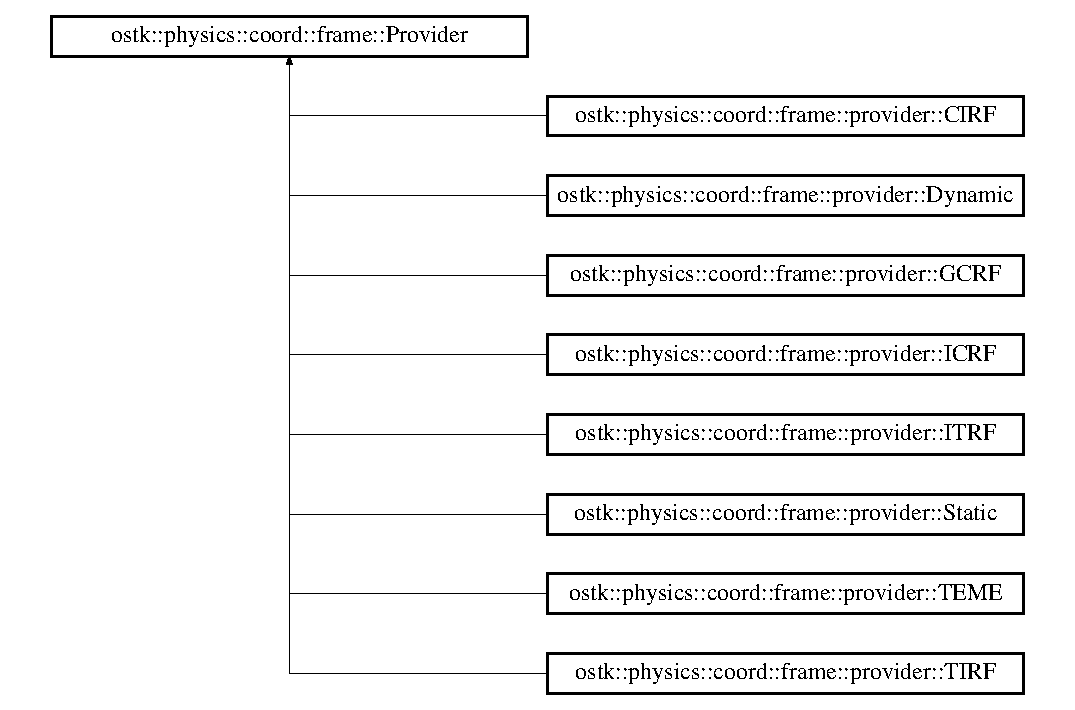
\includegraphics[height=9.000000cm]{classostk_1_1physics_1_1coord_1_1frame_1_1_provider}
\end{center}
\end{figure}
\subsection*{Public Member Functions}
\begin{DoxyCompactItemize}
\item 
\hyperlink{classostk_1_1physics_1_1coord_1_1frame_1_1_provider_a627a13fa73073656b2d0b3bd81e0423e}{Provider} ()
\item 
virtual \hyperlink{classostk_1_1physics_1_1coord_1_1frame_1_1_provider_a6d84675199cb79c56de9189e91dbfe81}{$\sim$\+Provider} ()=0
\item 
virtual \hyperlink{classostk_1_1physics_1_1coord_1_1frame_1_1_provider}{Provider} $\ast$ \hyperlink{classostk_1_1physics_1_1coord_1_1frame_1_1_provider_ae41bc3862d088e9c8d90a79253294ce9}{clone} () const =0
\item 
virtual bool \hyperlink{classostk_1_1physics_1_1coord_1_1frame_1_1_provider_a27acab0012649796b97956fed1a91493}{is\+Defined} () const =0
\item 
virtual \hyperlink{classostk_1_1physics_1_1coord_1_1_transform}{Transform} \hyperlink{classostk_1_1physics_1_1coord_1_1frame_1_1_provider_a38b86a589f46f8b8a9c97ab2776f37d1}{get\+Transform\+At} (const \hyperlink{classostk_1_1physics_1_1time_1_1_instant}{Instant} \&an\+Instant) const =0
\end{DoxyCompactItemize}


\subsection{Detailed Description}
\hyperlink{classostk_1_1physics_1_1coord_1_1_frame}{Frame} provider. 

\subsection{Constructor \& Destructor Documentation}
\mbox{\Hypertarget{classostk_1_1physics_1_1coord_1_1frame_1_1_provider_a627a13fa73073656b2d0b3bd81e0423e}\label{classostk_1_1physics_1_1coord_1_1frame_1_1_provider_a627a13fa73073656b2d0b3bd81e0423e}} 
\index{ostk\+::physics\+::coord\+::frame\+::\+Provider@{ostk\+::physics\+::coord\+::frame\+::\+Provider}!Provider@{Provider}}
\index{Provider@{Provider}!ostk\+::physics\+::coord\+::frame\+::\+Provider@{ostk\+::physics\+::coord\+::frame\+::\+Provider}}
\subsubsection{\texorpdfstring{Provider()}{Provider()}}
{\footnotesize\ttfamily ostk\+::physics\+::coord\+::frame\+::\+Provider\+::\+Provider (\begin{DoxyParamCaption}{ }\end{DoxyParamCaption})}

\mbox{\Hypertarget{classostk_1_1physics_1_1coord_1_1frame_1_1_provider_a6d84675199cb79c56de9189e91dbfe81}\label{classostk_1_1physics_1_1coord_1_1frame_1_1_provider_a6d84675199cb79c56de9189e91dbfe81}} 
\index{ostk\+::physics\+::coord\+::frame\+::\+Provider@{ostk\+::physics\+::coord\+::frame\+::\+Provider}!````~Provider@{$\sim$\+Provider}}
\index{````~Provider@{$\sim$\+Provider}!ostk\+::physics\+::coord\+::frame\+::\+Provider@{ostk\+::physics\+::coord\+::frame\+::\+Provider}}
\subsubsection{\texorpdfstring{$\sim$\+Provider()}{~Provider()}}
{\footnotesize\ttfamily ostk\+::physics\+::coord\+::frame\+::\+Provider\+::$\sim$\+Provider (\begin{DoxyParamCaption}{ }\end{DoxyParamCaption})\hspace{0.3cm}{\ttfamily [pure virtual]}}



\subsection{Member Function Documentation}
\mbox{\Hypertarget{classostk_1_1physics_1_1coord_1_1frame_1_1_provider_ae41bc3862d088e9c8d90a79253294ce9}\label{classostk_1_1physics_1_1coord_1_1frame_1_1_provider_ae41bc3862d088e9c8d90a79253294ce9}} 
\index{ostk\+::physics\+::coord\+::frame\+::\+Provider@{ostk\+::physics\+::coord\+::frame\+::\+Provider}!clone@{clone}}
\index{clone@{clone}!ostk\+::physics\+::coord\+::frame\+::\+Provider@{ostk\+::physics\+::coord\+::frame\+::\+Provider}}
\subsubsection{\texorpdfstring{clone()}{clone()}}
{\footnotesize\ttfamily virtual \hyperlink{classostk_1_1physics_1_1coord_1_1frame_1_1_provider}{Provider}$\ast$ ostk\+::physics\+::coord\+::frame\+::\+Provider\+::clone (\begin{DoxyParamCaption}{ }\end{DoxyParamCaption}) const\hspace{0.3cm}{\ttfamily [pure virtual]}}



Implemented in \hyperlink{classostk_1_1physics_1_1coord_1_1frame_1_1provider_1_1_c_i_r_f_a9c7c1e79785b676501e6a4686389a425}{ostk\+::physics\+::coord\+::frame\+::provider\+::\+C\+I\+RF}, \hyperlink{classostk_1_1physics_1_1coord_1_1frame_1_1provider_1_1_t_e_m_e_a10031d843340adafe7d9f4a3a0a4f86c}{ostk\+::physics\+::coord\+::frame\+::provider\+::\+T\+E\+ME}, \hyperlink{classostk_1_1physics_1_1coord_1_1frame_1_1provider_1_1_t_i_r_f_ae29e3db5bd1bccbc69a507f8716b73e5}{ostk\+::physics\+::coord\+::frame\+::provider\+::\+T\+I\+RF}, \hyperlink{classostk_1_1physics_1_1coord_1_1frame_1_1provider_1_1_dynamic_a37623142581671606ea45ca3bda0d0c8}{ostk\+::physics\+::coord\+::frame\+::provider\+::\+Dynamic}, \hyperlink{classostk_1_1physics_1_1coord_1_1frame_1_1provider_1_1_g_c_r_f_a71f14cba2d0d20a5bbeaa3b4fb08a79a}{ostk\+::physics\+::coord\+::frame\+::provider\+::\+G\+C\+RF}, \hyperlink{classostk_1_1physics_1_1coord_1_1frame_1_1provider_1_1_i_c_r_f_a40f7812d39719db68178ab6850a5cdde}{ostk\+::physics\+::coord\+::frame\+::provider\+::\+I\+C\+RF}, \hyperlink{classostk_1_1physics_1_1coord_1_1frame_1_1provider_1_1_i_t_r_f_aad7e29329b68f264bed571bf48b902a4}{ostk\+::physics\+::coord\+::frame\+::provider\+::\+I\+T\+RF}, and \hyperlink{classostk_1_1physics_1_1coord_1_1frame_1_1provider_1_1_static_a3e25a6fc979fc4ac28d8cbea4835ea71}{ostk\+::physics\+::coord\+::frame\+::provider\+::\+Static}.

\mbox{\Hypertarget{classostk_1_1physics_1_1coord_1_1frame_1_1_provider_a38b86a589f46f8b8a9c97ab2776f37d1}\label{classostk_1_1physics_1_1coord_1_1frame_1_1_provider_a38b86a589f46f8b8a9c97ab2776f37d1}} 
\index{ostk\+::physics\+::coord\+::frame\+::\+Provider@{ostk\+::physics\+::coord\+::frame\+::\+Provider}!get\+Transform\+At@{get\+Transform\+At}}
\index{get\+Transform\+At@{get\+Transform\+At}!ostk\+::physics\+::coord\+::frame\+::\+Provider@{ostk\+::physics\+::coord\+::frame\+::\+Provider}}
\subsubsection{\texorpdfstring{get\+Transform\+At()}{getTransformAt()}}
{\footnotesize\ttfamily virtual \hyperlink{classostk_1_1physics_1_1coord_1_1_transform}{Transform} ostk\+::physics\+::coord\+::frame\+::\+Provider\+::get\+Transform\+At (\begin{DoxyParamCaption}\item[{const \hyperlink{classostk_1_1physics_1_1time_1_1_instant}{Instant} \&}]{an\+Instant }\end{DoxyParamCaption}) const\hspace{0.3cm}{\ttfamily [pure virtual]}}



Implemented in \hyperlink{classostk_1_1physics_1_1coord_1_1frame_1_1provider_1_1_c_i_r_f_a9a9cdbec164d2f54cfdaa2a1a62c3250}{ostk\+::physics\+::coord\+::frame\+::provider\+::\+C\+I\+RF}, \hyperlink{classostk_1_1physics_1_1coord_1_1frame_1_1provider_1_1_t_e_m_e_a167738db76b74c42d29c0edbded94e51}{ostk\+::physics\+::coord\+::frame\+::provider\+::\+T\+E\+ME}, \hyperlink{classostk_1_1physics_1_1coord_1_1frame_1_1provider_1_1_t_i_r_f_a23d651ab9857ad748e6bf3815205cd72}{ostk\+::physics\+::coord\+::frame\+::provider\+::\+T\+I\+RF}, \hyperlink{classostk_1_1physics_1_1coord_1_1frame_1_1provider_1_1_dynamic_a7b7bfc8957fd84d90d0479944a427005}{ostk\+::physics\+::coord\+::frame\+::provider\+::\+Dynamic}, \hyperlink{classostk_1_1physics_1_1coord_1_1frame_1_1provider_1_1_g_c_r_f_a379dffe2291d4536dbdd65501fd28539}{ostk\+::physics\+::coord\+::frame\+::provider\+::\+G\+C\+RF}, \hyperlink{classostk_1_1physics_1_1coord_1_1frame_1_1provider_1_1_i_c_r_f_ab8d3ba4c098340eb43583e80cb5dd826}{ostk\+::physics\+::coord\+::frame\+::provider\+::\+I\+C\+RF}, \hyperlink{classostk_1_1physics_1_1coord_1_1frame_1_1provider_1_1_i_t_r_f_a6e344e7252a962d4451e2c0ea866bc30}{ostk\+::physics\+::coord\+::frame\+::provider\+::\+I\+T\+RF}, and \hyperlink{classostk_1_1physics_1_1coord_1_1frame_1_1provider_1_1_static_a0fbed95f9f17a51aca6d8f83c9532510}{ostk\+::physics\+::coord\+::frame\+::provider\+::\+Static}.

\mbox{\Hypertarget{classostk_1_1physics_1_1coord_1_1frame_1_1_provider_a27acab0012649796b97956fed1a91493}\label{classostk_1_1physics_1_1coord_1_1frame_1_1_provider_a27acab0012649796b97956fed1a91493}} 
\index{ostk\+::physics\+::coord\+::frame\+::\+Provider@{ostk\+::physics\+::coord\+::frame\+::\+Provider}!is\+Defined@{is\+Defined}}
\index{is\+Defined@{is\+Defined}!ostk\+::physics\+::coord\+::frame\+::\+Provider@{ostk\+::physics\+::coord\+::frame\+::\+Provider}}
\subsubsection{\texorpdfstring{is\+Defined()}{isDefined()}}
{\footnotesize\ttfamily virtual bool ostk\+::physics\+::coord\+::frame\+::\+Provider\+::is\+Defined (\begin{DoxyParamCaption}{ }\end{DoxyParamCaption}) const\hspace{0.3cm}{\ttfamily [pure virtual]}}



Implemented in \hyperlink{classostk_1_1physics_1_1coord_1_1frame_1_1provider_1_1_c_i_r_f_affec3924a864a0d793ee5aa887a06cf8}{ostk\+::physics\+::coord\+::frame\+::provider\+::\+C\+I\+RF}, \hyperlink{classostk_1_1physics_1_1coord_1_1frame_1_1provider_1_1_t_e_m_e_a8a1c5599411f152c63b69819e89b0464}{ostk\+::physics\+::coord\+::frame\+::provider\+::\+T\+E\+ME}, \hyperlink{classostk_1_1physics_1_1coord_1_1frame_1_1provider_1_1_t_i_r_f_ac7f3d815a45e270adab07bf6f51dc25f}{ostk\+::physics\+::coord\+::frame\+::provider\+::\+T\+I\+RF}, \hyperlink{classostk_1_1physics_1_1coord_1_1frame_1_1provider_1_1_dynamic_ab01d8d9a09df8e46680eb1acb830a86c}{ostk\+::physics\+::coord\+::frame\+::provider\+::\+Dynamic}, \hyperlink{classostk_1_1physics_1_1coord_1_1frame_1_1provider_1_1_g_c_r_f_a02160b74124b3ece74912c62aae5caaa}{ostk\+::physics\+::coord\+::frame\+::provider\+::\+G\+C\+RF}, \hyperlink{classostk_1_1physics_1_1coord_1_1frame_1_1provider_1_1_i_c_r_f_a0d8e56478597e46dbc2c1867e6774398}{ostk\+::physics\+::coord\+::frame\+::provider\+::\+I\+C\+RF}, \hyperlink{classostk_1_1physics_1_1coord_1_1frame_1_1provider_1_1_i_t_r_f_a2f3a53b002d54f1adf829cefc2cf7393}{ostk\+::physics\+::coord\+::frame\+::provider\+::\+I\+T\+RF}, and \hyperlink{classostk_1_1physics_1_1coord_1_1frame_1_1provider_1_1_static_a5b7189d8cff8128fee348af2feac1304}{ostk\+::physics\+::coord\+::frame\+::provider\+::\+Static}.



The documentation for this class was generated from the following files\+:\begin{DoxyCompactItemize}
\item 
include/\+Open\+Space\+Toolkit/\+Physics/\+Coordinate/\+Frame/\hyperlink{_provider_8hpp}{Provider.\+hpp}\item 
src/\+Open\+Space\+Toolkit/\+Physics/\+Coordinate/\+Frame/\hyperlink{_provider_8cpp}{Provider.\+cpp}\end{DoxyCompactItemize}

\hypertarget{classostk_1_1physics_1_1data_1_1_scalar}{}\section{ostk\+:\+:physics\+:\+:data\+:\+:Scalar Class Reference}
\label{classostk_1_1physics_1_1data_1_1_scalar}\index{ostk\+::physics\+::data\+::\+Scalar@{ostk\+::physics\+::data\+::\+Scalar}}


\hyperlink{classostk_1_1physics_1_1data_1_1_scalar}{Scalar} quantity.  




{\ttfamily \#include $<$Scalar.\+hpp$>$}

\subsection*{Public Member Functions}
\begin{DoxyCompactItemize}
\item 
\hyperlink{classostk_1_1physics_1_1data_1_1_scalar_a9c81732bf949003d9a613680d183c3af}{Scalar} (const Real \&a\+Value, const \hyperlink{classostk_1_1physics_1_1_unit}{Unit} \&a\+Unit)
\item 
bool \hyperlink{classostk_1_1physics_1_1data_1_1_scalar_a92a4f3e75436e61c077c6d8b37198e95}{operator==} (const \hyperlink{classostk_1_1physics_1_1data_1_1_scalar}{Scalar} \&a\+Scalar) const
\item 
bool \hyperlink{classostk_1_1physics_1_1data_1_1_scalar_a9d1f401cb3df5a6621c1fc04d86ce423}{operator!=} (const \hyperlink{classostk_1_1physics_1_1data_1_1_scalar}{Scalar} \&a\+Scalar) const
\item 
bool \hyperlink{classostk_1_1physics_1_1data_1_1_scalar_a93ea853416cca1007c462ffafdd4aa95}{is\+Defined} () const
\item 
Real \hyperlink{classostk_1_1physics_1_1data_1_1_scalar_ab632ef637308f3b97f0ab4ef63780e54}{get\+Value} () const
\item 
\hyperlink{classostk_1_1physics_1_1_unit}{Unit} \hyperlink{classostk_1_1physics_1_1data_1_1_scalar_af2bf59b6c0681b8770083006328ecdd5}{get\+Unit} () const
\item 
\hyperlink{classostk_1_1physics_1_1data_1_1_scalar}{Scalar} \hyperlink{classostk_1_1physics_1_1data_1_1_scalar_abe53604aa68b58737d7ffbf039a018f3}{in\+Unit} (const \hyperlink{classostk_1_1physics_1_1_unit}{Unit} \&a\+Unit) const
\item 
String \hyperlink{classostk_1_1physics_1_1data_1_1_scalar_acc184e1d5fa8e7868fcb67e065e68b77}{to\+String} (const Integer \&a\+Precision=Integer\+::\+Undefined()) const
\end{DoxyCompactItemize}
\subsection*{Static Public Member Functions}
\begin{DoxyCompactItemize}
\item 
static \hyperlink{classostk_1_1physics_1_1data_1_1_scalar}{Scalar} \hyperlink{classostk_1_1physics_1_1data_1_1_scalar_a5f261e9c75633f5fa0ac5b5d892241fe}{Undefined} ()
\end{DoxyCompactItemize}
\subsection*{Friends}
\begin{DoxyCompactItemize}
\item 
std\+::ostream \& \hyperlink{classostk_1_1physics_1_1data_1_1_scalar_ac5e6ec203257e2dbec9f528ff111aa52}{operator$<$$<$} (std\+::ostream \&an\+Output\+Stream, const \hyperlink{classostk_1_1physics_1_1data_1_1_scalar}{Scalar} \&a\+Scalar)
\end{DoxyCompactItemize}


\subsection{Detailed Description}
\hyperlink{classostk_1_1physics_1_1data_1_1_scalar}{Scalar} quantity. 

A scalar quantity is a physical quantity that can be described by a single element of a number field such as a real number, often accompanied by units of measurement.

https\+://en.wikipedia.\+org/wiki/\+Scalar\+\_\+(physics) 

\subsection{Constructor \& Destructor Documentation}
\mbox{\Hypertarget{classostk_1_1physics_1_1data_1_1_scalar_a9c81732bf949003d9a613680d183c3af}\label{classostk_1_1physics_1_1data_1_1_scalar_a9c81732bf949003d9a613680d183c3af}} 
\index{ostk\+::physics\+::data\+::\+Scalar@{ostk\+::physics\+::data\+::\+Scalar}!Scalar@{Scalar}}
\index{Scalar@{Scalar}!ostk\+::physics\+::data\+::\+Scalar@{ostk\+::physics\+::data\+::\+Scalar}}
\subsubsection{\texorpdfstring{Scalar()}{Scalar()}}
{\footnotesize\ttfamily ostk\+::physics\+::data\+::\+Scalar\+::\+Scalar (\begin{DoxyParamCaption}\item[{const Real \&}]{a\+Value,  }\item[{const \hyperlink{classostk_1_1physics_1_1_unit}{Unit} \&}]{a\+Unit }\end{DoxyParamCaption})}



\subsection{Member Function Documentation}
\mbox{\Hypertarget{classostk_1_1physics_1_1data_1_1_scalar_af2bf59b6c0681b8770083006328ecdd5}\label{classostk_1_1physics_1_1data_1_1_scalar_af2bf59b6c0681b8770083006328ecdd5}} 
\index{ostk\+::physics\+::data\+::\+Scalar@{ostk\+::physics\+::data\+::\+Scalar}!get\+Unit@{get\+Unit}}
\index{get\+Unit@{get\+Unit}!ostk\+::physics\+::data\+::\+Scalar@{ostk\+::physics\+::data\+::\+Scalar}}
\subsubsection{\texorpdfstring{get\+Unit()}{getUnit()}}
{\footnotesize\ttfamily \hyperlink{classostk_1_1physics_1_1_unit}{Unit} ostk\+::physics\+::data\+::\+Scalar\+::get\+Unit (\begin{DoxyParamCaption}{ }\end{DoxyParamCaption}) const}

\mbox{\Hypertarget{classostk_1_1physics_1_1data_1_1_scalar_ab632ef637308f3b97f0ab4ef63780e54}\label{classostk_1_1physics_1_1data_1_1_scalar_ab632ef637308f3b97f0ab4ef63780e54}} 
\index{ostk\+::physics\+::data\+::\+Scalar@{ostk\+::physics\+::data\+::\+Scalar}!get\+Value@{get\+Value}}
\index{get\+Value@{get\+Value}!ostk\+::physics\+::data\+::\+Scalar@{ostk\+::physics\+::data\+::\+Scalar}}
\subsubsection{\texorpdfstring{get\+Value()}{getValue()}}
{\footnotesize\ttfamily Real ostk\+::physics\+::data\+::\+Scalar\+::get\+Value (\begin{DoxyParamCaption}{ }\end{DoxyParamCaption}) const}

\mbox{\Hypertarget{classostk_1_1physics_1_1data_1_1_scalar_abe53604aa68b58737d7ffbf039a018f3}\label{classostk_1_1physics_1_1data_1_1_scalar_abe53604aa68b58737d7ffbf039a018f3}} 
\index{ostk\+::physics\+::data\+::\+Scalar@{ostk\+::physics\+::data\+::\+Scalar}!in\+Unit@{in\+Unit}}
\index{in\+Unit@{in\+Unit}!ostk\+::physics\+::data\+::\+Scalar@{ostk\+::physics\+::data\+::\+Scalar}}
\subsubsection{\texorpdfstring{in\+Unit()}{inUnit()}}
{\footnotesize\ttfamily \hyperlink{classostk_1_1physics_1_1data_1_1_scalar}{Scalar} ostk\+::physics\+::data\+::\+Scalar\+::in\+Unit (\begin{DoxyParamCaption}\item[{const \hyperlink{classostk_1_1physics_1_1_unit}{Unit} \&}]{a\+Unit }\end{DoxyParamCaption}) const}

\mbox{\Hypertarget{classostk_1_1physics_1_1data_1_1_scalar_a93ea853416cca1007c462ffafdd4aa95}\label{classostk_1_1physics_1_1data_1_1_scalar_a93ea853416cca1007c462ffafdd4aa95}} 
\index{ostk\+::physics\+::data\+::\+Scalar@{ostk\+::physics\+::data\+::\+Scalar}!is\+Defined@{is\+Defined}}
\index{is\+Defined@{is\+Defined}!ostk\+::physics\+::data\+::\+Scalar@{ostk\+::physics\+::data\+::\+Scalar}}
\subsubsection{\texorpdfstring{is\+Defined()}{isDefined()}}
{\footnotesize\ttfamily bool ostk\+::physics\+::data\+::\+Scalar\+::is\+Defined (\begin{DoxyParamCaption}{ }\end{DoxyParamCaption}) const}

\mbox{\Hypertarget{classostk_1_1physics_1_1data_1_1_scalar_a9d1f401cb3df5a6621c1fc04d86ce423}\label{classostk_1_1physics_1_1data_1_1_scalar_a9d1f401cb3df5a6621c1fc04d86ce423}} 
\index{ostk\+::physics\+::data\+::\+Scalar@{ostk\+::physics\+::data\+::\+Scalar}!operator"!=@{operator"!=}}
\index{operator"!=@{operator"!=}!ostk\+::physics\+::data\+::\+Scalar@{ostk\+::physics\+::data\+::\+Scalar}}
\subsubsection{\texorpdfstring{operator"!=()}{operator!=()}}
{\footnotesize\ttfamily bool ostk\+::physics\+::data\+::\+Scalar\+::operator!= (\begin{DoxyParamCaption}\item[{const \hyperlink{classostk_1_1physics_1_1data_1_1_scalar}{Scalar} \&}]{a\+Scalar }\end{DoxyParamCaption}) const}

\mbox{\Hypertarget{classostk_1_1physics_1_1data_1_1_scalar_a92a4f3e75436e61c077c6d8b37198e95}\label{classostk_1_1physics_1_1data_1_1_scalar_a92a4f3e75436e61c077c6d8b37198e95}} 
\index{ostk\+::physics\+::data\+::\+Scalar@{ostk\+::physics\+::data\+::\+Scalar}!operator==@{operator==}}
\index{operator==@{operator==}!ostk\+::physics\+::data\+::\+Scalar@{ostk\+::physics\+::data\+::\+Scalar}}
\subsubsection{\texorpdfstring{operator==()}{operator==()}}
{\footnotesize\ttfamily bool ostk\+::physics\+::data\+::\+Scalar\+::operator== (\begin{DoxyParamCaption}\item[{const \hyperlink{classostk_1_1physics_1_1data_1_1_scalar}{Scalar} \&}]{a\+Scalar }\end{DoxyParamCaption}) const}

\mbox{\Hypertarget{classostk_1_1physics_1_1data_1_1_scalar_acc184e1d5fa8e7868fcb67e065e68b77}\label{classostk_1_1physics_1_1data_1_1_scalar_acc184e1d5fa8e7868fcb67e065e68b77}} 
\index{ostk\+::physics\+::data\+::\+Scalar@{ostk\+::physics\+::data\+::\+Scalar}!to\+String@{to\+String}}
\index{to\+String@{to\+String}!ostk\+::physics\+::data\+::\+Scalar@{ostk\+::physics\+::data\+::\+Scalar}}
\subsubsection{\texorpdfstring{to\+String()}{toString()}}
{\footnotesize\ttfamily String ostk\+::physics\+::data\+::\+Scalar\+::to\+String (\begin{DoxyParamCaption}\item[{const Integer \&}]{a\+Precision = {\ttfamily Integer\+:\+:Undefined()} }\end{DoxyParamCaption}) const}

\mbox{\Hypertarget{classostk_1_1physics_1_1data_1_1_scalar_a5f261e9c75633f5fa0ac5b5d892241fe}\label{classostk_1_1physics_1_1data_1_1_scalar_a5f261e9c75633f5fa0ac5b5d892241fe}} 
\index{ostk\+::physics\+::data\+::\+Scalar@{ostk\+::physics\+::data\+::\+Scalar}!Undefined@{Undefined}}
\index{Undefined@{Undefined}!ostk\+::physics\+::data\+::\+Scalar@{ostk\+::physics\+::data\+::\+Scalar}}
\subsubsection{\texorpdfstring{Undefined()}{Undefined()}}
{\footnotesize\ttfamily \hyperlink{classostk_1_1physics_1_1data_1_1_scalar}{Scalar} ostk\+::physics\+::data\+::\+Scalar\+::\+Undefined (\begin{DoxyParamCaption}{ }\end{DoxyParamCaption})\hspace{0.3cm}{\ttfamily [static]}}



\subsection{Friends And Related Function Documentation}
\mbox{\Hypertarget{classostk_1_1physics_1_1data_1_1_scalar_ac5e6ec203257e2dbec9f528ff111aa52}\label{classostk_1_1physics_1_1data_1_1_scalar_ac5e6ec203257e2dbec9f528ff111aa52}} 
\index{ostk\+::physics\+::data\+::\+Scalar@{ostk\+::physics\+::data\+::\+Scalar}!operator$<$$<$@{operator$<$$<$}}
\index{operator$<$$<$@{operator$<$$<$}!ostk\+::physics\+::data\+::\+Scalar@{ostk\+::physics\+::data\+::\+Scalar}}
\subsubsection{\texorpdfstring{operator$<$$<$}{operator<<}}
{\footnotesize\ttfamily std\+::ostream\& operator$<$$<$ (\begin{DoxyParamCaption}\item[{std\+::ostream \&}]{an\+Output\+Stream,  }\item[{const \hyperlink{classostk_1_1physics_1_1data_1_1_scalar}{Scalar} \&}]{a\+Scalar }\end{DoxyParamCaption})\hspace{0.3cm}{\ttfamily [friend]}}



The documentation for this class was generated from the following files\+:\begin{DoxyCompactItemize}
\item 
include/\+Open\+Space\+Toolkit/\+Physics/\+Data/\hyperlink{_scalar_8hpp}{Scalar.\+hpp}\item 
src/\+Open\+Space\+Toolkit/\+Physics/\+Data/\hyperlink{_scalar_8cpp}{Scalar.\+cpp}\end{DoxyCompactItemize}

\hypertarget{classostk_1_1physics_1_1environment_1_1gravitational_1_1_spherical}{}\section{ostk\+:\+:physics\+:\+:environment\+:\+:gravitational\+:\+:Spherical Class Reference}
\label{classostk_1_1physics_1_1environment_1_1gravitational_1_1_spherical}\index{ostk\+::physics\+::environment\+::gravitational\+::\+Spherical@{ostk\+::physics\+::environment\+::gravitational\+::\+Spherical}}


\hyperlink{classostk_1_1physics_1_1environment_1_1gravitational_1_1_spherical}{Spherical} gravitational model.  




{\ttfamily \#include $<$Spherical.\+hpp$>$}

Inheritance diagram for ostk\+:\+:physics\+:\+:environment\+:\+:gravitational\+:\+:Spherical\+:\begin{figure}[H]
\begin{center}
\leavevmode
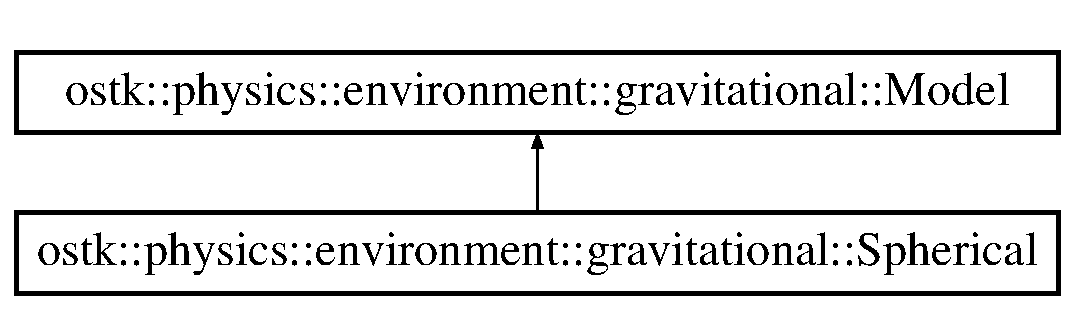
\includegraphics[height=2.000000cm]{classostk_1_1physics_1_1environment_1_1gravitational_1_1_spherical}
\end{center}
\end{figure}
\subsection*{Public Member Functions}
\begin{DoxyCompactItemize}
\item 
\hyperlink{classostk_1_1physics_1_1environment_1_1gravitational_1_1_spherical_aa0181210c54a42a0b6e808d6e6811d6b}{Spherical} (const \hyperlink{classostk_1_1physics_1_1units_1_1_derived}{Derived} \&a\+Gravitational\+Parameter)
\begin{DoxyCompactList}\small\item\em Constructor. \end{DoxyCompactList}\item 
virtual \hyperlink{classostk_1_1physics_1_1environment_1_1gravitational_1_1_spherical}{Spherical} $\ast$ \hyperlink{classostk_1_1physics_1_1environment_1_1gravitational_1_1_spherical_ac9f63de9656589a27a77e7a8d48836bd}{clone} () const override
\begin{DoxyCompactList}\small\item\em Clone the spherical gravitational model. \end{DoxyCompactList}\item 
virtual Vector3d \hyperlink{classostk_1_1physics_1_1environment_1_1gravitational_1_1_spherical_a37243cf671418b0cb9eff229101b5e96}{get\+Field\+Value\+At} (const Vector3d \&a\+Position, const \hyperlink{classostk_1_1physics_1_1time_1_1_instant}{Instant} \&an\+Instant) const override
\begin{DoxyCompactList}\small\item\em Get the gravitational field value at a given position and instant. \end{DoxyCompactList}\end{DoxyCompactItemize}


\subsection{Detailed Description}
\hyperlink{classostk_1_1physics_1_1environment_1_1gravitational_1_1_spherical}{Spherical} gravitational model. 

\subsection{Constructor \& Destructor Documentation}
\mbox{\Hypertarget{classostk_1_1physics_1_1environment_1_1gravitational_1_1_spherical_aa0181210c54a42a0b6e808d6e6811d6b}\label{classostk_1_1physics_1_1environment_1_1gravitational_1_1_spherical_aa0181210c54a42a0b6e808d6e6811d6b}} 
\index{ostk\+::physics\+::environment\+::gravitational\+::\+Spherical@{ostk\+::physics\+::environment\+::gravitational\+::\+Spherical}!Spherical@{Spherical}}
\index{Spherical@{Spherical}!ostk\+::physics\+::environment\+::gravitational\+::\+Spherical@{ostk\+::physics\+::environment\+::gravitational\+::\+Spherical}}
\subsubsection{\texorpdfstring{Spherical()}{Spherical()}}
{\footnotesize\ttfamily ostk\+::physics\+::environment\+::gravitational\+::\+Spherical\+::\+Spherical (\begin{DoxyParamCaption}\item[{const \hyperlink{classostk_1_1physics_1_1units_1_1_derived}{Derived} \&}]{a\+Gravitational\+Parameter }\end{DoxyParamCaption})}



Constructor. 


\begin{DoxyParams}[1]{Parameters}
\mbox{\tt in}  & {\em a\+Gravitational\+Parameter} & A gravitational parameter \\
\hline
\end{DoxyParams}


\subsection{Member Function Documentation}
\mbox{\Hypertarget{classostk_1_1physics_1_1environment_1_1gravitational_1_1_spherical_ac9f63de9656589a27a77e7a8d48836bd}\label{classostk_1_1physics_1_1environment_1_1gravitational_1_1_spherical_ac9f63de9656589a27a77e7a8d48836bd}} 
\index{ostk\+::physics\+::environment\+::gravitational\+::\+Spherical@{ostk\+::physics\+::environment\+::gravitational\+::\+Spherical}!clone@{clone}}
\index{clone@{clone}!ostk\+::physics\+::environment\+::gravitational\+::\+Spherical@{ostk\+::physics\+::environment\+::gravitational\+::\+Spherical}}
\subsubsection{\texorpdfstring{clone()}{clone()}}
{\footnotesize\ttfamily \hyperlink{classostk_1_1physics_1_1environment_1_1gravitational_1_1_spherical}{Spherical} $\ast$ ostk\+::physics\+::environment\+::gravitational\+::\+Spherical\+::clone (\begin{DoxyParamCaption}{ }\end{DoxyParamCaption}) const\hspace{0.3cm}{\ttfamily [override]}, {\ttfamily [virtual]}}



Clone the spherical gravitational model. 

\begin{DoxyReturn}{Returns}
Pointer to spherical gravitational model 
\end{DoxyReturn}


Implements \hyperlink{classostk_1_1physics_1_1environment_1_1gravitational_1_1_model_a399257ac86e7f0112a702141e0e2e4a7}{ostk\+::physics\+::environment\+::gravitational\+::\+Model}.

\mbox{\Hypertarget{classostk_1_1physics_1_1environment_1_1gravitational_1_1_spherical_a37243cf671418b0cb9eff229101b5e96}\label{classostk_1_1physics_1_1environment_1_1gravitational_1_1_spherical_a37243cf671418b0cb9eff229101b5e96}} 
\index{ostk\+::physics\+::environment\+::gravitational\+::\+Spherical@{ostk\+::physics\+::environment\+::gravitational\+::\+Spherical}!get\+Field\+Value\+At@{get\+Field\+Value\+At}}
\index{get\+Field\+Value\+At@{get\+Field\+Value\+At}!ostk\+::physics\+::environment\+::gravitational\+::\+Spherical@{ostk\+::physics\+::environment\+::gravitational\+::\+Spherical}}
\subsubsection{\texorpdfstring{get\+Field\+Value\+At()}{getFieldValueAt()}}
{\footnotesize\ttfamily Vector3d ostk\+::physics\+::environment\+::gravitational\+::\+Spherical\+::get\+Field\+Value\+At (\begin{DoxyParamCaption}\item[{const Vector3d \&}]{a\+Position,  }\item[{const \hyperlink{classostk_1_1physics_1_1time_1_1_instant}{Instant} \&}]{an\+Instant }\end{DoxyParamCaption}) const\hspace{0.3cm}{\ttfamily [override]}, {\ttfamily [virtual]}}



Get the gravitational field value at a given position and instant. 


\begin{DoxyParams}[1]{Parameters}
\mbox{\tt in}  & {\em a\+Position} & A position, expressed in the gravitational object frame \mbox{[}m\mbox{]} \\
\hline
\mbox{\tt in}  & {\em an\+Instant} & An instant \\
\hline
\end{DoxyParams}
\begin{DoxyReturn}{Returns}
Gravitational field value, expressed in the gravitational object frame \mbox{[}m.\+s-\/2\mbox{]} 
\end{DoxyReturn}


Implements \hyperlink{classostk_1_1physics_1_1environment_1_1gravitational_1_1_model_a5ef3b4ddf4240e8a26553294fe392581}{ostk\+::physics\+::environment\+::gravitational\+::\+Model}.



The documentation for this class was generated from the following files\+:\begin{DoxyCompactItemize}
\item 
include/\+Open\+Space\+Toolkit/\+Physics/\+Environment/\+Gravitational/\hyperlink{_spherical_8hpp}{Spherical.\+hpp}\item 
src/\+Open\+Space\+Toolkit/\+Physics/\+Environment/\+Gravitational/\hyperlink{_spherical_8cpp}{Spherical.\+cpp}\end{DoxyCompactItemize}

\hypertarget{classostk_1_1physics_1_1env_1_1ephem_1_1_s_p_i_c_e}{}\section{ostk\+:\+:physics\+:\+:env\+:\+:ephem\+:\+:S\+P\+I\+CE Class Reference}
\label{classostk_1_1physics_1_1env_1_1ephem_1_1_s_p_i_c_e}\index{ostk\+::physics\+::env\+::ephem\+::\+S\+P\+I\+CE@{ostk\+::physics\+::env\+::ephem\+::\+S\+P\+I\+CE}}


\hyperlink{classostk_1_1physics_1_1env_1_1ephem_1_1_s_p_i_c_e}{S\+P\+I\+CE} Toolkit ephemeris.  




{\ttfamily \#include $<$S\+P\+I\+C\+E.\+hpp$>$}

Inheritance diagram for ostk\+:\+:physics\+:\+:env\+:\+:ephem\+:\+:S\+P\+I\+CE\+:\begin{figure}[H]
\begin{center}
\leavevmode
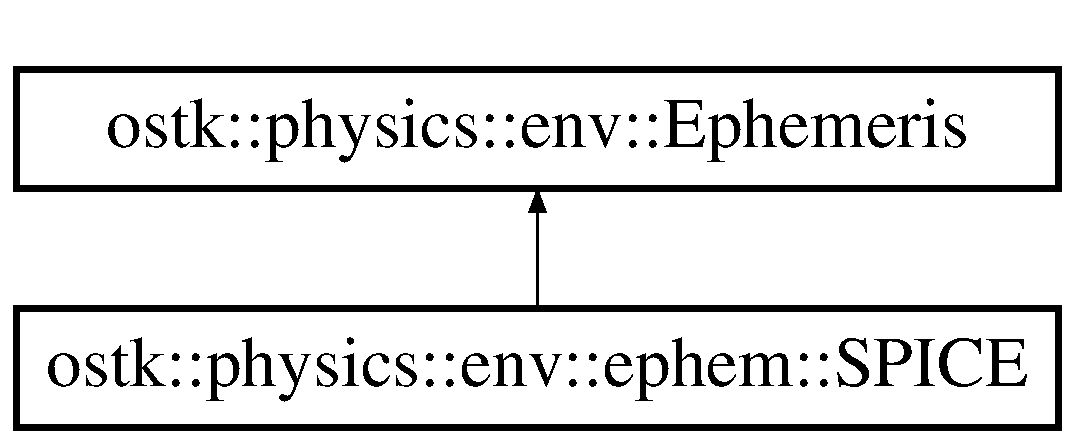
\includegraphics[height=2.000000cm]{classostk_1_1physics_1_1env_1_1ephem_1_1_s_p_i_c_e}
\end{center}
\end{figure}
\subsection*{Public Types}
\begin{DoxyCompactItemize}
\item 
enum \hyperlink{classostk_1_1physics_1_1env_1_1ephem_1_1_s_p_i_c_e_ae84db78d858cdd0a1dc3ff53090f4a1f}{Object} \{ \newline
\hyperlink{classostk_1_1physics_1_1env_1_1ephem_1_1_s_p_i_c_e_ae84db78d858cdd0a1dc3ff53090f4a1faec0fc0100c4fc1ce4eea230c3dc10360}{Object\+::\+Undefined}, 
\hyperlink{classostk_1_1physics_1_1env_1_1ephem_1_1_s_p_i_c_e_ae84db78d858cdd0a1dc3ff53090f4a1faef6572e4cd58bb39a3f4e82fc64fe9f0}{Object\+::\+Sun}, 
\hyperlink{classostk_1_1physics_1_1env_1_1ephem_1_1_s_p_i_c_e_ae84db78d858cdd0a1dc3ff53090f4a1fa34dae487e31f37aa74633258b7774d4f}{Object\+::\+Mercury}, 
\hyperlink{classostk_1_1physics_1_1env_1_1ephem_1_1_s_p_i_c_e_ae84db78d858cdd0a1dc3ff53090f4a1fa0bdc508a17811a3a860d32749ad44e4b}{Object\+::\+Venus}, 
\newline
\hyperlink{classostk_1_1physics_1_1env_1_1ephem_1_1_s_p_i_c_e_ae84db78d858cdd0a1dc3ff53090f4a1fa5cdd21c97f86686cc505e02fd32a7523}{Object\+::\+Earth}, 
\hyperlink{classostk_1_1physics_1_1env_1_1ephem_1_1_s_p_i_c_e_ae84db78d858cdd0a1dc3ff53090f4a1fad502a50ed945d5fca74e0105575b5b34}{Object\+::\+Moon}, 
\hyperlink{classostk_1_1physics_1_1env_1_1ephem_1_1_s_p_i_c_e_ae84db78d858cdd0a1dc3ff53090f4a1fa671f028142280b556a85ffdd90e0a43d}{Object\+::\+Mars}, 
\hyperlink{classostk_1_1physics_1_1env_1_1ephem_1_1_s_p_i_c_e_ae84db78d858cdd0a1dc3ff53090f4a1fa89c5c30498c2989611f9044be006197c}{Object\+::\+Jupiter}, 
\newline
\hyperlink{classostk_1_1physics_1_1env_1_1ephem_1_1_s_p_i_c_e_ae84db78d858cdd0a1dc3ff53090f4a1fa233ea1805dab5120a0ecc49b71a48063}{Object\+::\+Saturn}, 
\hyperlink{classostk_1_1physics_1_1env_1_1ephem_1_1_s_p_i_c_e_ae84db78d858cdd0a1dc3ff53090f4a1fa76b840d32f33267ad812507b47e3a1b5}{Object\+::\+Uranus}, 
\hyperlink{classostk_1_1physics_1_1env_1_1ephem_1_1_s_p_i_c_e_ae84db78d858cdd0a1dc3ff53090f4a1faf8d3b65d8479a31ebf67cb18dd0a4641}{Object\+::\+Neptune}
 \}\begin{DoxyCompactList}\small\item\em \hyperlink{classostk_1_1physics_1_1env_1_1ephem_1_1_s_p_i_c_e}{S\+P\+I\+CE} object. \end{DoxyCompactList}
\end{DoxyCompactItemize}
\subsection*{Public Member Functions}
\begin{DoxyCompactItemize}
\item 
\hyperlink{classostk_1_1physics_1_1env_1_1ephem_1_1_s_p_i_c_e_a47224d4625f6574ed2b9681f7bfa9c31}{S\+P\+I\+CE} (const \hyperlink{classostk_1_1physics_1_1env_1_1ephem_1_1_s_p_i_c_e_ae84db78d858cdd0a1dc3ff53090f4a1f}{S\+P\+I\+C\+E\+::\+Object} \&an\+Object)
\begin{DoxyCompactList}\small\item\em Constructor. \end{DoxyCompactList}\item 
virtual \hyperlink{classostk_1_1physics_1_1env_1_1ephem_1_1_s_p_i_c_e_abd2e7f60841f6600b4bca015dd50df3d}{$\sim$\+S\+P\+I\+CE} () override
\begin{DoxyCompactList}\small\item\em Destructor. \end{DoxyCompactList}\item 
virtual \hyperlink{classostk_1_1physics_1_1env_1_1ephem_1_1_s_p_i_c_e}{S\+P\+I\+CE} $\ast$ \hyperlink{classostk_1_1physics_1_1env_1_1ephem_1_1_s_p_i_c_e_af9155765c2546bd8707b56ed86f77c2d}{clone} () const override
\begin{DoxyCompactList}\small\item\em Clone. \end{DoxyCompactList}\item 
virtual bool \hyperlink{classostk_1_1physics_1_1env_1_1ephem_1_1_s_p_i_c_e_a2e5350a46c5efe938998b760ee783f77}{is\+Defined} () const override
\begin{DoxyCompactList}\small\item\em Returns true if \hyperlink{classostk_1_1physics_1_1env_1_1ephem_1_1_s_p_i_c_e}{S\+P\+I\+CE} is defined. \end{DoxyCompactList}\item 
virtual Shared$<$ const \hyperlink{classostk_1_1physics_1_1coord_1_1_frame}{Frame} $>$ \hyperlink{classostk_1_1physics_1_1env_1_1ephem_1_1_s_p_i_c_e_abf9dee32d47dbb1308af0c9783c84854}{access\+Frame} () const override
\begin{DoxyCompactList}\small\item\em Access frame of \hyperlink{classostk_1_1physics_1_1env_1_1ephem_1_1_s_p_i_c_e}{S\+P\+I\+CE} object. \end{DoxyCompactList}\end{DoxyCompactItemize}
\subsection*{Static Public Member Functions}
\begin{DoxyCompactItemize}
\item 
static String \hyperlink{classostk_1_1physics_1_1env_1_1ephem_1_1_s_p_i_c_e_a97570f88c117786553614fc42d1ac5ff}{String\+From\+Object} (const \hyperlink{classostk_1_1physics_1_1env_1_1ephem_1_1_s_p_i_c_e_ae84db78d858cdd0a1dc3ff53090f4a1f}{S\+P\+I\+C\+E\+::\+Object} \&an\+Object)
\begin{DoxyCompactList}\small\item\em Convert \hyperlink{classostk_1_1physics_1_1env_1_1ephem_1_1_s_p_i_c_e}{S\+P\+I\+CE} object to string. \end{DoxyCompactList}\end{DoxyCompactItemize}


\subsection{Detailed Description}
\hyperlink{classostk_1_1physics_1_1env_1_1ephem_1_1_s_p_i_c_e}{S\+P\+I\+CE} Toolkit ephemeris. 

https\+://en.wikipedia.\+org/wiki/\+Jet\+\_\+\+Propulsion\+\_\+\+Laboratory\+\_\+\+Development\+\_\+\+Ephemeris 

\subsection{Member Enumeration Documentation}
\mbox{\Hypertarget{classostk_1_1physics_1_1env_1_1ephem_1_1_s_p_i_c_e_ae84db78d858cdd0a1dc3ff53090f4a1f}\label{classostk_1_1physics_1_1env_1_1ephem_1_1_s_p_i_c_e_ae84db78d858cdd0a1dc3ff53090f4a1f}} 
\index{ostk\+::physics\+::env\+::ephem\+::\+S\+P\+I\+CE@{ostk\+::physics\+::env\+::ephem\+::\+S\+P\+I\+CE}!Object@{Object}}
\index{Object@{Object}!ostk\+::physics\+::env\+::ephem\+::\+S\+P\+I\+CE@{ostk\+::physics\+::env\+::ephem\+::\+S\+P\+I\+CE}}
\subsubsection{\texorpdfstring{Object}{Object}}
{\footnotesize\ttfamily enum \hyperlink{classostk_1_1physics_1_1env_1_1ephem_1_1_s_p_i_c_e_ae84db78d858cdd0a1dc3ff53090f4a1f}{ostk\+::physics\+::env\+::ephem\+::\+S\+P\+I\+C\+E\+::\+Object}\hspace{0.3cm}{\ttfamily [strong]}}



\hyperlink{classostk_1_1physics_1_1env_1_1ephem_1_1_s_p_i_c_e}{S\+P\+I\+CE} object. 

\begin{DoxyEnumFields}{Enumerator}
\raisebox{\heightof{T}}[0pt][0pt]{\index{Undefined@{Undefined}!ostk\+::physics\+::env\+::ephem\+::\+S\+P\+I\+CE@{ostk\+::physics\+::env\+::ephem\+::\+S\+P\+I\+CE}}\index{ostk\+::physics\+::env\+::ephem\+::\+S\+P\+I\+CE@{ostk\+::physics\+::env\+::ephem\+::\+S\+P\+I\+CE}!Undefined@{Undefined}}}\mbox{\Hypertarget{classostk_1_1physics_1_1env_1_1ephem_1_1_s_p_i_c_e_ae84db78d858cdd0a1dc3ff53090f4a1faec0fc0100c4fc1ce4eea230c3dc10360}\label{classostk_1_1physics_1_1env_1_1ephem_1_1_s_p_i_c_e_ae84db78d858cdd0a1dc3ff53090f4a1faec0fc0100c4fc1ce4eea230c3dc10360}} 
Undefined&\\
\hline

\raisebox{\heightof{T}}[0pt][0pt]{\index{Sun@{Sun}!ostk\+::physics\+::env\+::ephem\+::\+S\+P\+I\+CE@{ostk\+::physics\+::env\+::ephem\+::\+S\+P\+I\+CE}}\index{ostk\+::physics\+::env\+::ephem\+::\+S\+P\+I\+CE@{ostk\+::physics\+::env\+::ephem\+::\+S\+P\+I\+CE}!Sun@{Sun}}}\mbox{\Hypertarget{classostk_1_1physics_1_1env_1_1ephem_1_1_s_p_i_c_e_ae84db78d858cdd0a1dc3ff53090f4a1faef6572e4cd58bb39a3f4e82fc64fe9f0}\label{classostk_1_1physics_1_1env_1_1ephem_1_1_s_p_i_c_e_ae84db78d858cdd0a1dc3ff53090f4a1faef6572e4cd58bb39a3f4e82fc64fe9f0}} 
Sun&\\
\hline

\raisebox{\heightof{T}}[0pt][0pt]{\index{Mercury@{Mercury}!ostk\+::physics\+::env\+::ephem\+::\+S\+P\+I\+CE@{ostk\+::physics\+::env\+::ephem\+::\+S\+P\+I\+CE}}\index{ostk\+::physics\+::env\+::ephem\+::\+S\+P\+I\+CE@{ostk\+::physics\+::env\+::ephem\+::\+S\+P\+I\+CE}!Mercury@{Mercury}}}\mbox{\Hypertarget{classostk_1_1physics_1_1env_1_1ephem_1_1_s_p_i_c_e_ae84db78d858cdd0a1dc3ff53090f4a1fa34dae487e31f37aa74633258b7774d4f}\label{classostk_1_1physics_1_1env_1_1ephem_1_1_s_p_i_c_e_ae84db78d858cdd0a1dc3ff53090f4a1fa34dae487e31f37aa74633258b7774d4f}} 
Mercury&\\
\hline

\raisebox{\heightof{T}}[0pt][0pt]{\index{Venus@{Venus}!ostk\+::physics\+::env\+::ephem\+::\+S\+P\+I\+CE@{ostk\+::physics\+::env\+::ephem\+::\+S\+P\+I\+CE}}\index{ostk\+::physics\+::env\+::ephem\+::\+S\+P\+I\+CE@{ostk\+::physics\+::env\+::ephem\+::\+S\+P\+I\+CE}!Venus@{Venus}}}\mbox{\Hypertarget{classostk_1_1physics_1_1env_1_1ephem_1_1_s_p_i_c_e_ae84db78d858cdd0a1dc3ff53090f4a1fa0bdc508a17811a3a860d32749ad44e4b}\label{classostk_1_1physics_1_1env_1_1ephem_1_1_s_p_i_c_e_ae84db78d858cdd0a1dc3ff53090f4a1fa0bdc508a17811a3a860d32749ad44e4b}} 
Venus&\\
\hline

\raisebox{\heightof{T}}[0pt][0pt]{\index{Earth@{Earth}!ostk\+::physics\+::env\+::ephem\+::\+S\+P\+I\+CE@{ostk\+::physics\+::env\+::ephem\+::\+S\+P\+I\+CE}}\index{ostk\+::physics\+::env\+::ephem\+::\+S\+P\+I\+CE@{ostk\+::physics\+::env\+::ephem\+::\+S\+P\+I\+CE}!Earth@{Earth}}}\mbox{\Hypertarget{classostk_1_1physics_1_1env_1_1ephem_1_1_s_p_i_c_e_ae84db78d858cdd0a1dc3ff53090f4a1fa5cdd21c97f86686cc505e02fd32a7523}\label{classostk_1_1physics_1_1env_1_1ephem_1_1_s_p_i_c_e_ae84db78d858cdd0a1dc3ff53090f4a1fa5cdd21c97f86686cc505e02fd32a7523}} 
Earth&\\
\hline

\raisebox{\heightof{T}}[0pt][0pt]{\index{Moon@{Moon}!ostk\+::physics\+::env\+::ephem\+::\+S\+P\+I\+CE@{ostk\+::physics\+::env\+::ephem\+::\+S\+P\+I\+CE}}\index{ostk\+::physics\+::env\+::ephem\+::\+S\+P\+I\+CE@{ostk\+::physics\+::env\+::ephem\+::\+S\+P\+I\+CE}!Moon@{Moon}}}\mbox{\Hypertarget{classostk_1_1physics_1_1env_1_1ephem_1_1_s_p_i_c_e_ae84db78d858cdd0a1dc3ff53090f4a1fad502a50ed945d5fca74e0105575b5b34}\label{classostk_1_1physics_1_1env_1_1ephem_1_1_s_p_i_c_e_ae84db78d858cdd0a1dc3ff53090f4a1fad502a50ed945d5fca74e0105575b5b34}} 
Moon&\\
\hline

\raisebox{\heightof{T}}[0pt][0pt]{\index{Mars@{Mars}!ostk\+::physics\+::env\+::ephem\+::\+S\+P\+I\+CE@{ostk\+::physics\+::env\+::ephem\+::\+S\+P\+I\+CE}}\index{ostk\+::physics\+::env\+::ephem\+::\+S\+P\+I\+CE@{ostk\+::physics\+::env\+::ephem\+::\+S\+P\+I\+CE}!Mars@{Mars}}}\mbox{\Hypertarget{classostk_1_1physics_1_1env_1_1ephem_1_1_s_p_i_c_e_ae84db78d858cdd0a1dc3ff53090f4a1fa671f028142280b556a85ffdd90e0a43d}\label{classostk_1_1physics_1_1env_1_1ephem_1_1_s_p_i_c_e_ae84db78d858cdd0a1dc3ff53090f4a1fa671f028142280b556a85ffdd90e0a43d}} 
Mars&\\
\hline

\raisebox{\heightof{T}}[0pt][0pt]{\index{Jupiter@{Jupiter}!ostk\+::physics\+::env\+::ephem\+::\+S\+P\+I\+CE@{ostk\+::physics\+::env\+::ephem\+::\+S\+P\+I\+CE}}\index{ostk\+::physics\+::env\+::ephem\+::\+S\+P\+I\+CE@{ostk\+::physics\+::env\+::ephem\+::\+S\+P\+I\+CE}!Jupiter@{Jupiter}}}\mbox{\Hypertarget{classostk_1_1physics_1_1env_1_1ephem_1_1_s_p_i_c_e_ae84db78d858cdd0a1dc3ff53090f4a1fa89c5c30498c2989611f9044be006197c}\label{classostk_1_1physics_1_1env_1_1ephem_1_1_s_p_i_c_e_ae84db78d858cdd0a1dc3ff53090f4a1fa89c5c30498c2989611f9044be006197c}} 
Jupiter&\\
\hline

\raisebox{\heightof{T}}[0pt][0pt]{\index{Saturn@{Saturn}!ostk\+::physics\+::env\+::ephem\+::\+S\+P\+I\+CE@{ostk\+::physics\+::env\+::ephem\+::\+S\+P\+I\+CE}}\index{ostk\+::physics\+::env\+::ephem\+::\+S\+P\+I\+CE@{ostk\+::physics\+::env\+::ephem\+::\+S\+P\+I\+CE}!Saturn@{Saturn}}}\mbox{\Hypertarget{classostk_1_1physics_1_1env_1_1ephem_1_1_s_p_i_c_e_ae84db78d858cdd0a1dc3ff53090f4a1fa233ea1805dab5120a0ecc49b71a48063}\label{classostk_1_1physics_1_1env_1_1ephem_1_1_s_p_i_c_e_ae84db78d858cdd0a1dc3ff53090f4a1fa233ea1805dab5120a0ecc49b71a48063}} 
Saturn&\\
\hline

\raisebox{\heightof{T}}[0pt][0pt]{\index{Uranus@{Uranus}!ostk\+::physics\+::env\+::ephem\+::\+S\+P\+I\+CE@{ostk\+::physics\+::env\+::ephem\+::\+S\+P\+I\+CE}}\index{ostk\+::physics\+::env\+::ephem\+::\+S\+P\+I\+CE@{ostk\+::physics\+::env\+::ephem\+::\+S\+P\+I\+CE}!Uranus@{Uranus}}}\mbox{\Hypertarget{classostk_1_1physics_1_1env_1_1ephem_1_1_s_p_i_c_e_ae84db78d858cdd0a1dc3ff53090f4a1fa76b840d32f33267ad812507b47e3a1b5}\label{classostk_1_1physics_1_1env_1_1ephem_1_1_s_p_i_c_e_ae84db78d858cdd0a1dc3ff53090f4a1fa76b840d32f33267ad812507b47e3a1b5}} 
Uranus&\\
\hline

\raisebox{\heightof{T}}[0pt][0pt]{\index{Neptune@{Neptune}!ostk\+::physics\+::env\+::ephem\+::\+S\+P\+I\+CE@{ostk\+::physics\+::env\+::ephem\+::\+S\+P\+I\+CE}}\index{ostk\+::physics\+::env\+::ephem\+::\+S\+P\+I\+CE@{ostk\+::physics\+::env\+::ephem\+::\+S\+P\+I\+CE}!Neptune@{Neptune}}}\mbox{\Hypertarget{classostk_1_1physics_1_1env_1_1ephem_1_1_s_p_i_c_e_ae84db78d858cdd0a1dc3ff53090f4a1faf8d3b65d8479a31ebf67cb18dd0a4641}\label{classostk_1_1physics_1_1env_1_1ephem_1_1_s_p_i_c_e_ae84db78d858cdd0a1dc3ff53090f4a1faf8d3b65d8479a31ebf67cb18dd0a4641}} 
Neptune&\\
\hline

\end{DoxyEnumFields}


\subsection{Constructor \& Destructor Documentation}
\mbox{\Hypertarget{classostk_1_1physics_1_1env_1_1ephem_1_1_s_p_i_c_e_a47224d4625f6574ed2b9681f7bfa9c31}\label{classostk_1_1physics_1_1env_1_1ephem_1_1_s_p_i_c_e_a47224d4625f6574ed2b9681f7bfa9c31}} 
\index{ostk\+::physics\+::env\+::ephem\+::\+S\+P\+I\+CE@{ostk\+::physics\+::env\+::ephem\+::\+S\+P\+I\+CE}!S\+P\+I\+CE@{S\+P\+I\+CE}}
\index{S\+P\+I\+CE@{S\+P\+I\+CE}!ostk\+::physics\+::env\+::ephem\+::\+S\+P\+I\+CE@{ostk\+::physics\+::env\+::ephem\+::\+S\+P\+I\+CE}}
\subsubsection{\texorpdfstring{S\+P\+I\+C\+E()}{SPICE()}}
{\footnotesize\ttfamily ostk\+::physics\+::env\+::ephem\+::\+S\+P\+I\+C\+E\+::\+S\+P\+I\+CE (\begin{DoxyParamCaption}\item[{const \hyperlink{classostk_1_1physics_1_1env_1_1ephem_1_1_s_p_i_c_e_ae84db78d858cdd0a1dc3ff53090f4a1f}{S\+P\+I\+C\+E\+::\+Object} \&}]{an\+Object }\end{DoxyParamCaption})}



Constructor. 


\begin{DoxyParams}[1]{Parameters}
\mbox{\tt in}  & {\em an\+Object} & A \hyperlink{classostk_1_1physics_1_1env_1_1ephem_1_1_s_p_i_c_e}{S\+P\+I\+CE} object \\
\hline
\end{DoxyParams}
\mbox{\Hypertarget{classostk_1_1physics_1_1env_1_1ephem_1_1_s_p_i_c_e_abd2e7f60841f6600b4bca015dd50df3d}\label{classostk_1_1physics_1_1env_1_1ephem_1_1_s_p_i_c_e_abd2e7f60841f6600b4bca015dd50df3d}} 
\index{ostk\+::physics\+::env\+::ephem\+::\+S\+P\+I\+CE@{ostk\+::physics\+::env\+::ephem\+::\+S\+P\+I\+CE}!````~S\+P\+I\+CE@{$\sim$\+S\+P\+I\+CE}}
\index{````~S\+P\+I\+CE@{$\sim$\+S\+P\+I\+CE}!ostk\+::physics\+::env\+::ephem\+::\+S\+P\+I\+CE@{ostk\+::physics\+::env\+::ephem\+::\+S\+P\+I\+CE}}
\subsubsection{\texorpdfstring{$\sim$\+S\+P\+I\+C\+E()}{~SPICE()}}
{\footnotesize\ttfamily ostk\+::physics\+::env\+::ephem\+::\+S\+P\+I\+C\+E\+::$\sim$\+S\+P\+I\+CE (\begin{DoxyParamCaption}{ }\end{DoxyParamCaption})\hspace{0.3cm}{\ttfamily [override]}, {\ttfamily [virtual]}}



Destructor. 



\subsection{Member Function Documentation}
\mbox{\Hypertarget{classostk_1_1physics_1_1env_1_1ephem_1_1_s_p_i_c_e_abf9dee32d47dbb1308af0c9783c84854}\label{classostk_1_1physics_1_1env_1_1ephem_1_1_s_p_i_c_e_abf9dee32d47dbb1308af0c9783c84854}} 
\index{ostk\+::physics\+::env\+::ephem\+::\+S\+P\+I\+CE@{ostk\+::physics\+::env\+::ephem\+::\+S\+P\+I\+CE}!access\+Frame@{access\+Frame}}
\index{access\+Frame@{access\+Frame}!ostk\+::physics\+::env\+::ephem\+::\+S\+P\+I\+CE@{ostk\+::physics\+::env\+::ephem\+::\+S\+P\+I\+CE}}
\subsubsection{\texorpdfstring{access\+Frame()}{accessFrame()}}
{\footnotesize\ttfamily Shared$<$ const \hyperlink{classostk_1_1physics_1_1coord_1_1_frame}{Frame} $>$ ostk\+::physics\+::env\+::ephem\+::\+S\+P\+I\+C\+E\+::access\+Frame (\begin{DoxyParamCaption}{ }\end{DoxyParamCaption}) const\hspace{0.3cm}{\ttfamily [override]}, {\ttfamily [virtual]}}



Access frame of \hyperlink{classostk_1_1physics_1_1env_1_1ephem_1_1_s_p_i_c_e}{S\+P\+I\+CE} object. 

\begin{DoxyReturn}{Returns}
Shared pointer to frame 
\end{DoxyReturn}


Implements \hyperlink{classostk_1_1physics_1_1env_1_1_ephemeris_a7a2e78c90901d813311d51d66fcf12bf}{ostk\+::physics\+::env\+::\+Ephemeris}.

\mbox{\Hypertarget{classostk_1_1physics_1_1env_1_1ephem_1_1_s_p_i_c_e_af9155765c2546bd8707b56ed86f77c2d}\label{classostk_1_1physics_1_1env_1_1ephem_1_1_s_p_i_c_e_af9155765c2546bd8707b56ed86f77c2d}} 
\index{ostk\+::physics\+::env\+::ephem\+::\+S\+P\+I\+CE@{ostk\+::physics\+::env\+::ephem\+::\+S\+P\+I\+CE}!clone@{clone}}
\index{clone@{clone}!ostk\+::physics\+::env\+::ephem\+::\+S\+P\+I\+CE@{ostk\+::physics\+::env\+::ephem\+::\+S\+P\+I\+CE}}
\subsubsection{\texorpdfstring{clone()}{clone()}}
{\footnotesize\ttfamily \hyperlink{classostk_1_1physics_1_1env_1_1ephem_1_1_s_p_i_c_e}{S\+P\+I\+CE} $\ast$ ostk\+::physics\+::env\+::ephem\+::\+S\+P\+I\+C\+E\+::clone (\begin{DoxyParamCaption}{ }\end{DoxyParamCaption}) const\hspace{0.3cm}{\ttfamily [override]}, {\ttfamily [virtual]}}



Clone. 

\begin{DoxyReturn}{Returns}
Pointer to \hyperlink{classostk_1_1physics_1_1env_1_1ephem_1_1_s_p_i_c_e}{S\+P\+I\+CE} 
\end{DoxyReturn}


Implements \hyperlink{classostk_1_1physics_1_1env_1_1_ephemeris_a3a35daaff1359882ae16b69ab6e399f6}{ostk\+::physics\+::env\+::\+Ephemeris}.

\mbox{\Hypertarget{classostk_1_1physics_1_1env_1_1ephem_1_1_s_p_i_c_e_a2e5350a46c5efe938998b760ee783f77}\label{classostk_1_1physics_1_1env_1_1ephem_1_1_s_p_i_c_e_a2e5350a46c5efe938998b760ee783f77}} 
\index{ostk\+::physics\+::env\+::ephem\+::\+S\+P\+I\+CE@{ostk\+::physics\+::env\+::ephem\+::\+S\+P\+I\+CE}!is\+Defined@{is\+Defined}}
\index{is\+Defined@{is\+Defined}!ostk\+::physics\+::env\+::ephem\+::\+S\+P\+I\+CE@{ostk\+::physics\+::env\+::ephem\+::\+S\+P\+I\+CE}}
\subsubsection{\texorpdfstring{is\+Defined()}{isDefined()}}
{\footnotesize\ttfamily bool ostk\+::physics\+::env\+::ephem\+::\+S\+P\+I\+C\+E\+::is\+Defined (\begin{DoxyParamCaption}{ }\end{DoxyParamCaption}) const\hspace{0.3cm}{\ttfamily [override]}, {\ttfamily [virtual]}}



Returns true if \hyperlink{classostk_1_1physics_1_1env_1_1ephem_1_1_s_p_i_c_e}{S\+P\+I\+CE} is defined. 

\begin{DoxyReturn}{Returns}
True if \hyperlink{classostk_1_1physics_1_1env_1_1ephem_1_1_s_p_i_c_e}{S\+P\+I\+CE} is defined 
\end{DoxyReturn}


Implements \hyperlink{classostk_1_1physics_1_1env_1_1_ephemeris_ace5a637a5f25f700dfe1a2cef2b08162}{ostk\+::physics\+::env\+::\+Ephemeris}.

\mbox{\Hypertarget{classostk_1_1physics_1_1env_1_1ephem_1_1_s_p_i_c_e_a97570f88c117786553614fc42d1ac5ff}\label{classostk_1_1physics_1_1env_1_1ephem_1_1_s_p_i_c_e_a97570f88c117786553614fc42d1ac5ff}} 
\index{ostk\+::physics\+::env\+::ephem\+::\+S\+P\+I\+CE@{ostk\+::physics\+::env\+::ephem\+::\+S\+P\+I\+CE}!String\+From\+Object@{String\+From\+Object}}
\index{String\+From\+Object@{String\+From\+Object}!ostk\+::physics\+::env\+::ephem\+::\+S\+P\+I\+CE@{ostk\+::physics\+::env\+::ephem\+::\+S\+P\+I\+CE}}
\subsubsection{\texorpdfstring{String\+From\+Object()}{StringFromObject()}}
{\footnotesize\ttfamily String ostk\+::physics\+::env\+::ephem\+::\+S\+P\+I\+C\+E\+::\+String\+From\+Object (\begin{DoxyParamCaption}\item[{const \hyperlink{classostk_1_1physics_1_1env_1_1ephem_1_1_s_p_i_c_e_ae84db78d858cdd0a1dc3ff53090f4a1f}{S\+P\+I\+C\+E\+::\+Object} \&}]{an\+Object }\end{DoxyParamCaption})\hspace{0.3cm}{\ttfamily [static]}}



Convert \hyperlink{classostk_1_1physics_1_1env_1_1ephem_1_1_s_p_i_c_e}{S\+P\+I\+CE} object to string. 


\begin{DoxyParams}[1]{Parameters}
\mbox{\tt in}  & {\em an\+Object} & A \hyperlink{classostk_1_1physics_1_1env_1_1ephem_1_1_s_p_i_c_e}{S\+P\+I\+CE} object \\
\hline
\end{DoxyParams}
\begin{DoxyReturn}{Returns}
String representation of \hyperlink{classostk_1_1physics_1_1env_1_1ephem_1_1_s_p_i_c_e}{S\+P\+I\+CE} object 
\end{DoxyReturn}


The documentation for this class was generated from the following files\+:\begin{DoxyCompactItemize}
\item 
include/\+Open\+Space\+Toolkit/\+Physics/\+Environment/\+Ephemerides/\hyperlink{_s_p_i_c_e_8hpp}{S\+P\+I\+C\+E.\+hpp}\item 
src/\+Open\+Space\+Toolkit/\+Physics/\+Environment/\+Ephemerides/\hyperlink{_s_p_i_c_e_8cpp}{S\+P\+I\+C\+E.\+cpp}\end{DoxyCompactItemize}

\hypertarget{classostk_1_1physics_1_1coord_1_1frame_1_1provider_1_1_static}{}\section{ostk\+:\+:physics\+:\+:coord\+:\+:frame\+:\+:provider\+:\+:Static Class Reference}
\label{classostk_1_1physics_1_1coord_1_1frame_1_1provider_1_1_static}\index{ostk\+::physics\+::coord\+::frame\+::provider\+::\+Static@{ostk\+::physics\+::coord\+::frame\+::provider\+::\+Static}}


\hyperlink{classostk_1_1physics_1_1coord_1_1frame_1_1provider_1_1_static}{Static} provider.  




{\ttfamily \#include $<$Static.\+hpp$>$}

Inheritance diagram for ostk\+:\+:physics\+:\+:coord\+:\+:frame\+:\+:provider\+:\+:Static\+:\begin{figure}[H]
\begin{center}
\leavevmode
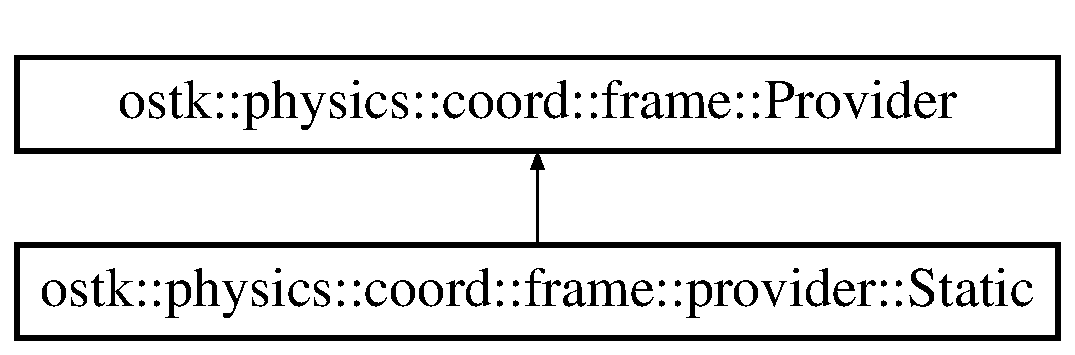
\includegraphics[height=2.000000cm]{classostk_1_1physics_1_1coord_1_1frame_1_1provider_1_1_static}
\end{center}
\end{figure}
\subsection*{Public Member Functions}
\begin{DoxyCompactItemize}
\item 
\hyperlink{classostk_1_1physics_1_1coord_1_1frame_1_1provider_1_1_static_a0526a2aa502a52e89f7d205c5b64e90c}{Static} (const \hyperlink{classostk_1_1physics_1_1coord_1_1_transform}{Transform} \&a\+Transform)
\item 
virtual \hyperlink{classostk_1_1physics_1_1coord_1_1frame_1_1provider_1_1_static_aa6ab7218047ee54f78825c75e821f2db}{$\sim$\+Static} () override
\item 
virtual \hyperlink{classostk_1_1physics_1_1coord_1_1frame_1_1provider_1_1_static}{Static} $\ast$ \hyperlink{classostk_1_1physics_1_1coord_1_1frame_1_1provider_1_1_static_a3e25a6fc979fc4ac28d8cbea4835ea71}{clone} () const override
\item 
virtual bool \hyperlink{classostk_1_1physics_1_1coord_1_1frame_1_1provider_1_1_static_a5b7189d8cff8128fee348af2feac1304}{is\+Defined} () const override
\item 
virtual \hyperlink{classostk_1_1physics_1_1coord_1_1_transform}{Transform} \hyperlink{classostk_1_1physics_1_1coord_1_1frame_1_1provider_1_1_static_a0fbed95f9f17a51aca6d8f83c9532510}{get\+Transform\+At} (const \hyperlink{classostk_1_1physics_1_1time_1_1_instant}{Instant} \&an\+Instant) const override
\end{DoxyCompactItemize}


\subsection{Detailed Description}
\hyperlink{classostk_1_1physics_1_1coord_1_1frame_1_1provider_1_1_static}{Static} provider. 

\subsection{Constructor \& Destructor Documentation}
\mbox{\Hypertarget{classostk_1_1physics_1_1coord_1_1frame_1_1provider_1_1_static_a0526a2aa502a52e89f7d205c5b64e90c}\label{classostk_1_1physics_1_1coord_1_1frame_1_1provider_1_1_static_a0526a2aa502a52e89f7d205c5b64e90c}} 
\index{ostk\+::physics\+::coord\+::frame\+::provider\+::\+Static@{ostk\+::physics\+::coord\+::frame\+::provider\+::\+Static}!Static@{Static}}
\index{Static@{Static}!ostk\+::physics\+::coord\+::frame\+::provider\+::\+Static@{ostk\+::physics\+::coord\+::frame\+::provider\+::\+Static}}
\subsubsection{\texorpdfstring{Static()}{Static()}}
{\footnotesize\ttfamily ostk\+::physics\+::coord\+::frame\+::provider\+::\+Static\+::\+Static (\begin{DoxyParamCaption}\item[{const \hyperlink{classostk_1_1physics_1_1coord_1_1_transform}{Transform} \&}]{a\+Transform }\end{DoxyParamCaption})}

\mbox{\Hypertarget{classostk_1_1physics_1_1coord_1_1frame_1_1provider_1_1_static_aa6ab7218047ee54f78825c75e821f2db}\label{classostk_1_1physics_1_1coord_1_1frame_1_1provider_1_1_static_aa6ab7218047ee54f78825c75e821f2db}} 
\index{ostk\+::physics\+::coord\+::frame\+::provider\+::\+Static@{ostk\+::physics\+::coord\+::frame\+::provider\+::\+Static}!````~Static@{$\sim$\+Static}}
\index{````~Static@{$\sim$\+Static}!ostk\+::physics\+::coord\+::frame\+::provider\+::\+Static@{ostk\+::physics\+::coord\+::frame\+::provider\+::\+Static}}
\subsubsection{\texorpdfstring{$\sim$\+Static()}{~Static()}}
{\footnotesize\ttfamily ostk\+::physics\+::coord\+::frame\+::provider\+::\+Static\+::$\sim$\+Static (\begin{DoxyParamCaption}{ }\end{DoxyParamCaption})\hspace{0.3cm}{\ttfamily [override]}, {\ttfamily [virtual]}}



\subsection{Member Function Documentation}
\mbox{\Hypertarget{classostk_1_1physics_1_1coord_1_1frame_1_1provider_1_1_static_a3e25a6fc979fc4ac28d8cbea4835ea71}\label{classostk_1_1physics_1_1coord_1_1frame_1_1provider_1_1_static_a3e25a6fc979fc4ac28d8cbea4835ea71}} 
\index{ostk\+::physics\+::coord\+::frame\+::provider\+::\+Static@{ostk\+::physics\+::coord\+::frame\+::provider\+::\+Static}!clone@{clone}}
\index{clone@{clone}!ostk\+::physics\+::coord\+::frame\+::provider\+::\+Static@{ostk\+::physics\+::coord\+::frame\+::provider\+::\+Static}}
\subsubsection{\texorpdfstring{clone()}{clone()}}
{\footnotesize\ttfamily \hyperlink{classostk_1_1physics_1_1coord_1_1frame_1_1provider_1_1_static}{Static} $\ast$ ostk\+::physics\+::coord\+::frame\+::provider\+::\+Static\+::clone (\begin{DoxyParamCaption}{ }\end{DoxyParamCaption}) const\hspace{0.3cm}{\ttfamily [override]}, {\ttfamily [virtual]}}



Implements \hyperlink{classostk_1_1physics_1_1coord_1_1frame_1_1_provider_ae41bc3862d088e9c8d90a79253294ce9}{ostk\+::physics\+::coord\+::frame\+::\+Provider}.

\mbox{\Hypertarget{classostk_1_1physics_1_1coord_1_1frame_1_1provider_1_1_static_a0fbed95f9f17a51aca6d8f83c9532510}\label{classostk_1_1physics_1_1coord_1_1frame_1_1provider_1_1_static_a0fbed95f9f17a51aca6d8f83c9532510}} 
\index{ostk\+::physics\+::coord\+::frame\+::provider\+::\+Static@{ostk\+::physics\+::coord\+::frame\+::provider\+::\+Static}!get\+Transform\+At@{get\+Transform\+At}}
\index{get\+Transform\+At@{get\+Transform\+At}!ostk\+::physics\+::coord\+::frame\+::provider\+::\+Static@{ostk\+::physics\+::coord\+::frame\+::provider\+::\+Static}}
\subsubsection{\texorpdfstring{get\+Transform\+At()}{getTransformAt()}}
{\footnotesize\ttfamily \hyperlink{classostk_1_1physics_1_1coord_1_1_transform}{Transform} ostk\+::physics\+::coord\+::frame\+::provider\+::\+Static\+::get\+Transform\+At (\begin{DoxyParamCaption}\item[{const \hyperlink{classostk_1_1physics_1_1time_1_1_instant}{Instant} \&}]{an\+Instant }\end{DoxyParamCaption}) const\hspace{0.3cm}{\ttfamily [override]}, {\ttfamily [virtual]}}



Implements \hyperlink{classostk_1_1physics_1_1coord_1_1frame_1_1_provider_a38b86a589f46f8b8a9c97ab2776f37d1}{ostk\+::physics\+::coord\+::frame\+::\+Provider}.

\mbox{\Hypertarget{classostk_1_1physics_1_1coord_1_1frame_1_1provider_1_1_static_a5b7189d8cff8128fee348af2feac1304}\label{classostk_1_1physics_1_1coord_1_1frame_1_1provider_1_1_static_a5b7189d8cff8128fee348af2feac1304}} 
\index{ostk\+::physics\+::coord\+::frame\+::provider\+::\+Static@{ostk\+::physics\+::coord\+::frame\+::provider\+::\+Static}!is\+Defined@{is\+Defined}}
\index{is\+Defined@{is\+Defined}!ostk\+::physics\+::coord\+::frame\+::provider\+::\+Static@{ostk\+::physics\+::coord\+::frame\+::provider\+::\+Static}}
\subsubsection{\texorpdfstring{is\+Defined()}{isDefined()}}
{\footnotesize\ttfamily bool ostk\+::physics\+::coord\+::frame\+::provider\+::\+Static\+::is\+Defined (\begin{DoxyParamCaption}{ }\end{DoxyParamCaption}) const\hspace{0.3cm}{\ttfamily [override]}, {\ttfamily [virtual]}}



Implements \hyperlink{classostk_1_1physics_1_1coord_1_1frame_1_1_provider_a27acab0012649796b97956fed1a91493}{ostk\+::physics\+::coord\+::frame\+::\+Provider}.



The documentation for this class was generated from the following files\+:\begin{DoxyCompactItemize}
\item 
include/\+Open\+Space\+Toolkit/\+Physics/\+Coordinate/\+Frame/\+Providers/\hyperlink{_static_8hpp}{Static.\+hpp}\item 
src/\+Open\+Space\+Toolkit/\+Physics/\+Coordinate/\+Frame/\+Providers/\hyperlink{_static_8cpp}{Static.\+cpp}\end{DoxyCompactItemize}

\hypertarget{classostk_1_1physics_1_1env_1_1obj_1_1celest_1_1_sun}{}\section{ostk\+:\+:physics\+:\+:env\+:\+:obj\+:\+:celest\+:\+:Sun Class Reference}
\label{classostk_1_1physics_1_1env_1_1obj_1_1celest_1_1_sun}\index{ostk\+::physics\+::env\+::obj\+::celest\+::\+Sun@{ostk\+::physics\+::env\+::obj\+::celest\+::\+Sun}}


{\ttfamily \#include $<$Sun.\+hpp$>$}

Inheritance diagram for ostk\+:\+:physics\+:\+:env\+:\+:obj\+:\+:celest\+:\+:Sun\+:\begin{figure}[H]
\begin{center}
\leavevmode
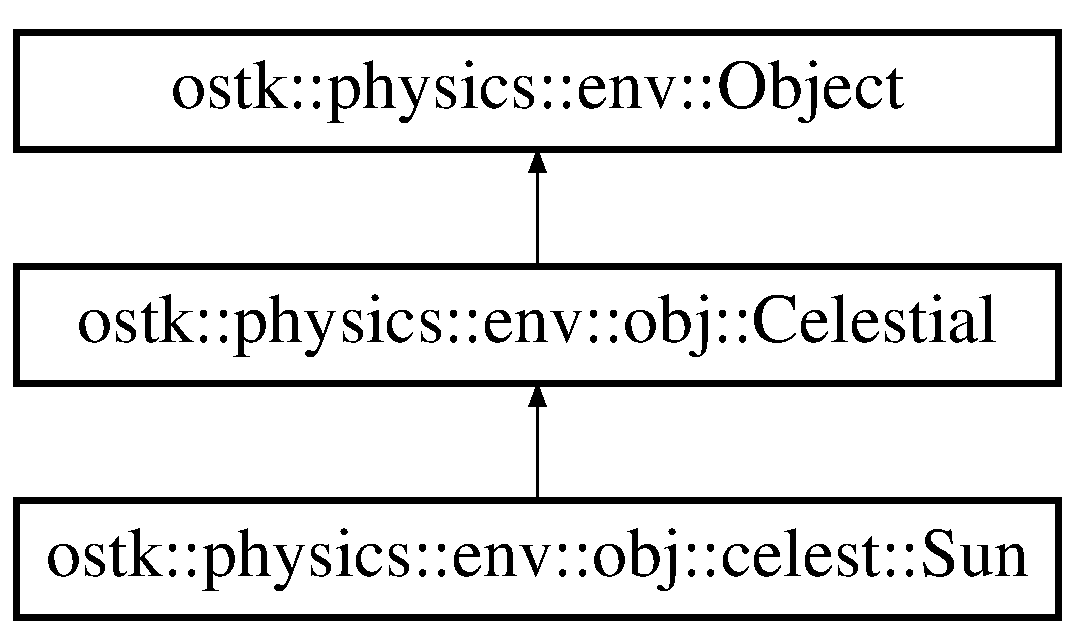
\includegraphics[height=3.000000cm]{classostk_1_1physics_1_1env_1_1obj_1_1celest_1_1_sun}
\end{center}
\end{figure}
\subsection*{Public Member Functions}
\begin{DoxyCompactItemize}
\item 
\hyperlink{classostk_1_1physics_1_1env_1_1obj_1_1celest_1_1_sun_ad2301582b97279e3ed9c91bca52a458e}{Sun} (const Shared$<$ \hyperlink{classostk_1_1physics_1_1env_1_1_ephemeris}{Ephemeris} $>$ \&an\+Ephemeris, const \hyperlink{classostk_1_1physics_1_1time_1_1_instant}{Instant} \&an\+Instant)
\item 
virtual \hyperlink{classostk_1_1physics_1_1env_1_1obj_1_1celest_1_1_sun_a1f4396f48b20848291a13f7033a14a58}{$\sim$\+Sun} () override
\item 
virtual \hyperlink{classostk_1_1physics_1_1env_1_1obj_1_1celest_1_1_sun}{Sun} $\ast$ \hyperlink{classostk_1_1physics_1_1env_1_1obj_1_1celest_1_1_sun_a57fd7c3c48115f77e2d3d331ef0e8e0a}{clone} () const override
\end{DoxyCompactItemize}
\subsection*{Static Public Member Functions}
\begin{DoxyCompactItemize}
\item 
static \hyperlink{classostk_1_1physics_1_1env_1_1obj_1_1celest_1_1_sun}{Sun} \hyperlink{classostk_1_1physics_1_1env_1_1obj_1_1celest_1_1_sun_afb5fc16a88e0f2bdbbb977ffb4263dbc}{Default} ()
\end{DoxyCompactItemize}
\subsection*{Static Public Attributes}
\begin{DoxyCompactItemize}
\item 
static \hyperlink{classostk_1_1physics_1_1units_1_1_derived}{Derived} \hyperlink{classostk_1_1physics_1_1env_1_1obj_1_1celest_1_1_sun_ab53baca68d9a8eaef2aa734011e29cc0}{Gravitational\+Parameter} = \{ 132712440018e9, Derived\+::\+Unit\+::\+Gravitational\+Parameter(\+Length\+::\+Unit\+::\+Meter, Time\+::\+Unit\+::\+Second) \}
\item 
static \hyperlink{classostk_1_1physics_1_1units_1_1_length}{Length} \hyperlink{classostk_1_1physics_1_1env_1_1obj_1_1celest_1_1_sun_a158d85a536619dc2f9550919a39b90a2}{Equatorial\+Radius} = \hyperlink{classostk_1_1physics_1_1units_1_1_length_ad227977ce00756791595796a0dd5ddd7}{Length\+::\+Meters}(6.\+955e8)
\item 
static Real \hyperlink{classostk_1_1physics_1_1env_1_1obj_1_1celest_1_1_sun_a04e467a3bb16cbaf9ec89cb63f556ddc}{Flattening} = 0.\+0
\end{DoxyCompactItemize}
\subsection*{Additional Inherited Members}


\subsection{Constructor \& Destructor Documentation}
\mbox{\Hypertarget{classostk_1_1physics_1_1env_1_1obj_1_1celest_1_1_sun_ad2301582b97279e3ed9c91bca52a458e}\label{classostk_1_1physics_1_1env_1_1obj_1_1celest_1_1_sun_ad2301582b97279e3ed9c91bca52a458e}} 
\index{ostk\+::physics\+::env\+::obj\+::celest\+::\+Sun@{ostk\+::physics\+::env\+::obj\+::celest\+::\+Sun}!Sun@{Sun}}
\index{Sun@{Sun}!ostk\+::physics\+::env\+::obj\+::celest\+::\+Sun@{ostk\+::physics\+::env\+::obj\+::celest\+::\+Sun}}
\subsubsection{\texorpdfstring{Sun()}{Sun()}}
{\footnotesize\ttfamily ostk\+::physics\+::env\+::obj\+::celest\+::\+Sun\+::\+Sun (\begin{DoxyParamCaption}\item[{const Shared$<$ \hyperlink{classostk_1_1physics_1_1env_1_1_ephemeris}{Ephemeris} $>$ \&}]{an\+Ephemeris,  }\item[{const \hyperlink{classostk_1_1physics_1_1time_1_1_instant}{Instant} \&}]{an\+Instant }\end{DoxyParamCaption})}

\mbox{\Hypertarget{classostk_1_1physics_1_1env_1_1obj_1_1celest_1_1_sun_a1f4396f48b20848291a13f7033a14a58}\label{classostk_1_1physics_1_1env_1_1obj_1_1celest_1_1_sun_a1f4396f48b20848291a13f7033a14a58}} 
\index{ostk\+::physics\+::env\+::obj\+::celest\+::\+Sun@{ostk\+::physics\+::env\+::obj\+::celest\+::\+Sun}!````~Sun@{$\sim$\+Sun}}
\index{````~Sun@{$\sim$\+Sun}!ostk\+::physics\+::env\+::obj\+::celest\+::\+Sun@{ostk\+::physics\+::env\+::obj\+::celest\+::\+Sun}}
\subsubsection{\texorpdfstring{$\sim$\+Sun()}{~Sun()}}
{\footnotesize\ttfamily ostk\+::physics\+::env\+::obj\+::celest\+::\+Sun\+::$\sim$\+Sun (\begin{DoxyParamCaption}{ }\end{DoxyParamCaption})\hspace{0.3cm}{\ttfamily [override]}, {\ttfamily [virtual]}}



\subsection{Member Function Documentation}
\mbox{\Hypertarget{classostk_1_1physics_1_1env_1_1obj_1_1celest_1_1_sun_a57fd7c3c48115f77e2d3d331ef0e8e0a}\label{classostk_1_1physics_1_1env_1_1obj_1_1celest_1_1_sun_a57fd7c3c48115f77e2d3d331ef0e8e0a}} 
\index{ostk\+::physics\+::env\+::obj\+::celest\+::\+Sun@{ostk\+::physics\+::env\+::obj\+::celest\+::\+Sun}!clone@{clone}}
\index{clone@{clone}!ostk\+::physics\+::env\+::obj\+::celest\+::\+Sun@{ostk\+::physics\+::env\+::obj\+::celest\+::\+Sun}}
\subsubsection{\texorpdfstring{clone()}{clone()}}
{\footnotesize\ttfamily \hyperlink{classostk_1_1physics_1_1env_1_1obj_1_1celest_1_1_sun}{Sun} $\ast$ ostk\+::physics\+::env\+::obj\+::celest\+::\+Sun\+::clone (\begin{DoxyParamCaption}{ }\end{DoxyParamCaption}) const\hspace{0.3cm}{\ttfamily [override]}, {\ttfamily [virtual]}}



Reimplemented from \hyperlink{classostk_1_1physics_1_1env_1_1obj_1_1_celestial_a87c6f3ec3c0ec9758ae52e3edc3fc5df}{ostk\+::physics\+::env\+::obj\+::\+Celestial}.

\mbox{\Hypertarget{classostk_1_1physics_1_1env_1_1obj_1_1celest_1_1_sun_afb5fc16a88e0f2bdbbb977ffb4263dbc}\label{classostk_1_1physics_1_1env_1_1obj_1_1celest_1_1_sun_afb5fc16a88e0f2bdbbb977ffb4263dbc}} 
\index{ostk\+::physics\+::env\+::obj\+::celest\+::\+Sun@{ostk\+::physics\+::env\+::obj\+::celest\+::\+Sun}!Default@{Default}}
\index{Default@{Default}!ostk\+::physics\+::env\+::obj\+::celest\+::\+Sun@{ostk\+::physics\+::env\+::obj\+::celest\+::\+Sun}}
\subsubsection{\texorpdfstring{Default()}{Default()}}
{\footnotesize\ttfamily \hyperlink{classostk_1_1physics_1_1env_1_1obj_1_1celest_1_1_sun}{Sun} ostk\+::physics\+::env\+::obj\+::celest\+::\+Sun\+::\+Default (\begin{DoxyParamCaption}{ }\end{DoxyParamCaption})\hspace{0.3cm}{\ttfamily [static]}}



\subsection{Member Data Documentation}
\mbox{\Hypertarget{classostk_1_1physics_1_1env_1_1obj_1_1celest_1_1_sun_a158d85a536619dc2f9550919a39b90a2}\label{classostk_1_1physics_1_1env_1_1obj_1_1celest_1_1_sun_a158d85a536619dc2f9550919a39b90a2}} 
\index{ostk\+::physics\+::env\+::obj\+::celest\+::\+Sun@{ostk\+::physics\+::env\+::obj\+::celest\+::\+Sun}!Equatorial\+Radius@{Equatorial\+Radius}}
\index{Equatorial\+Radius@{Equatorial\+Radius}!ostk\+::physics\+::env\+::obj\+::celest\+::\+Sun@{ostk\+::physics\+::env\+::obj\+::celest\+::\+Sun}}
\subsubsection{\texorpdfstring{Equatorial\+Radius}{EquatorialRadius}}
{\footnotesize\ttfamily \hyperlink{classostk_1_1physics_1_1units_1_1_length}{Length} ostk\+::physics\+::env\+::obj\+::celest\+::\+Sun\+::\+Equatorial\+Radius = \hyperlink{classostk_1_1physics_1_1units_1_1_length_ad227977ce00756791595796a0dd5ddd7}{Length\+::\+Meters}(6.\+955e8)\hspace{0.3cm}{\ttfamily [static]}}

\mbox{\Hypertarget{classostk_1_1physics_1_1env_1_1obj_1_1celest_1_1_sun_a04e467a3bb16cbaf9ec89cb63f556ddc}\label{classostk_1_1physics_1_1env_1_1obj_1_1celest_1_1_sun_a04e467a3bb16cbaf9ec89cb63f556ddc}} 
\index{ostk\+::physics\+::env\+::obj\+::celest\+::\+Sun@{ostk\+::physics\+::env\+::obj\+::celest\+::\+Sun}!Flattening@{Flattening}}
\index{Flattening@{Flattening}!ostk\+::physics\+::env\+::obj\+::celest\+::\+Sun@{ostk\+::physics\+::env\+::obj\+::celest\+::\+Sun}}
\subsubsection{\texorpdfstring{Flattening}{Flattening}}
{\footnotesize\ttfamily Real ostk\+::physics\+::env\+::obj\+::celest\+::\+Sun\+::\+Flattening = 0.\+0\hspace{0.3cm}{\ttfamily [static]}}

\mbox{\Hypertarget{classostk_1_1physics_1_1env_1_1obj_1_1celest_1_1_sun_ab53baca68d9a8eaef2aa734011e29cc0}\label{classostk_1_1physics_1_1env_1_1obj_1_1celest_1_1_sun_ab53baca68d9a8eaef2aa734011e29cc0}} 
\index{ostk\+::physics\+::env\+::obj\+::celest\+::\+Sun@{ostk\+::physics\+::env\+::obj\+::celest\+::\+Sun}!Gravitational\+Parameter@{Gravitational\+Parameter}}
\index{Gravitational\+Parameter@{Gravitational\+Parameter}!ostk\+::physics\+::env\+::obj\+::celest\+::\+Sun@{ostk\+::physics\+::env\+::obj\+::celest\+::\+Sun}}
\subsubsection{\texorpdfstring{Gravitational\+Parameter}{GravitationalParameter}}
{\footnotesize\ttfamily \hyperlink{classostk_1_1physics_1_1units_1_1_derived}{Derived} ostk\+::physics\+::env\+::obj\+::celest\+::\+Sun\+::\+Gravitational\+Parameter = \{ 132712440018e9, Derived\+::\+Unit\+::\+Gravitational\+Parameter(\+Length\+::\+Unit\+::\+Meter, Time\+::\+Unit\+::\+Second) \}\hspace{0.3cm}{\ttfamily [static]}}



The documentation for this class was generated from the following files\+:\begin{DoxyCompactItemize}
\item 
include/\+Open\+Space\+Toolkit/\+Physics/\+Environment/\+Objects/\+Celestial\+Bodies/\hyperlink{_sun_8hpp}{Sun.\+hpp}\item 
src/\+Open\+Space\+Toolkit/\+Physics/\+Environment/\+Objects/\+Celestial\+Bodies/\hyperlink{_sun_8cpp}{Sun.\+cpp}\end{DoxyCompactItemize}

\hypertarget{classostk_1_1physics_1_1coord_1_1frame_1_1provider_1_1_t_e_m_e}{}\section{ostk\+:\+:physics\+:\+:coord\+:\+:frame\+:\+:provider\+:\+:T\+E\+ME Class Reference}
\label{classostk_1_1physics_1_1coord_1_1frame_1_1provider_1_1_t_e_m_e}\index{ostk\+::physics\+::coord\+::frame\+::provider\+::\+T\+E\+ME@{ostk\+::physics\+::coord\+::frame\+::provider\+::\+T\+E\+ME}}


True Equator Mean Equinox (\hyperlink{classostk_1_1physics_1_1coord_1_1frame_1_1provider_1_1_t_e_m_e}{T\+E\+ME}) frame provider.  




{\ttfamily \#include $<$T\+E\+M\+E.\+hpp$>$}

Inheritance diagram for ostk\+:\+:physics\+:\+:coord\+:\+:frame\+:\+:provider\+:\+:T\+E\+ME\+:\begin{figure}[H]
\begin{center}
\leavevmode
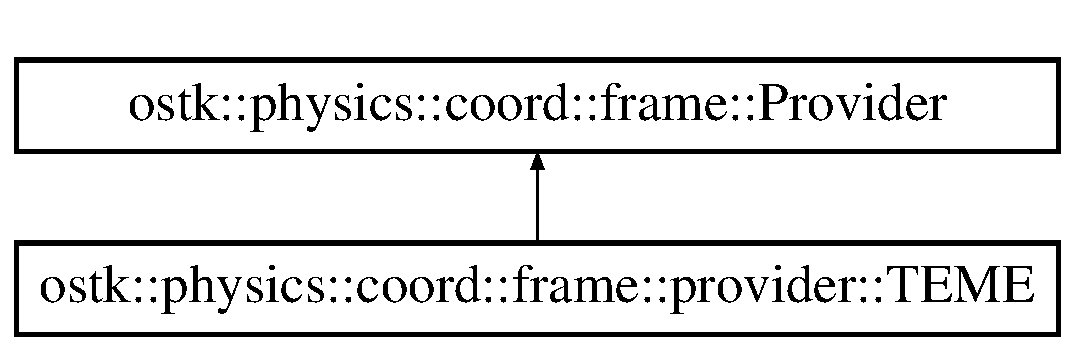
\includegraphics[height=2.000000cm]{classostk_1_1physics_1_1coord_1_1frame_1_1provider_1_1_t_e_m_e}
\end{center}
\end{figure}
\subsection*{Public Member Functions}
\begin{DoxyCompactItemize}
\item 
\hyperlink{classostk_1_1physics_1_1coord_1_1frame_1_1provider_1_1_t_e_m_e_a96f18f0fec3fa4ee10fc7a586d9bc01d}{T\+E\+ME} ()
\item 
virtual \hyperlink{classostk_1_1physics_1_1coord_1_1frame_1_1provider_1_1_t_e_m_e_aaea0539a9d40b1f805d1d8e6ee57dc74}{$\sim$\+T\+E\+ME} () override
\item 
virtual \hyperlink{classostk_1_1physics_1_1coord_1_1frame_1_1provider_1_1_t_e_m_e}{T\+E\+ME} $\ast$ \hyperlink{classostk_1_1physics_1_1coord_1_1frame_1_1provider_1_1_t_e_m_e_a10031d843340adafe7d9f4a3a0a4f86c}{clone} () const override
\item 
virtual bool \hyperlink{classostk_1_1physics_1_1coord_1_1frame_1_1provider_1_1_t_e_m_e_a8a1c5599411f152c63b69819e89b0464}{is\+Defined} () const override
\item 
virtual \hyperlink{classostk_1_1physics_1_1coord_1_1_transform}{Transform} \hyperlink{classostk_1_1physics_1_1coord_1_1frame_1_1provider_1_1_t_e_m_e_a167738db76b74c42d29c0edbded94e51}{get\+Transform\+At} (const \hyperlink{classostk_1_1physics_1_1time_1_1_instant}{Instant} \&an\+Instant) const override
\end{DoxyCompactItemize}


\subsection{Detailed Description}
True Equator Mean Equinox (\hyperlink{classostk_1_1physics_1_1coord_1_1frame_1_1provider_1_1_t_e_m_e}{T\+E\+ME}) frame provider. 

\begin{DoxyNote}{Note}
This frame should only be used with Two-\/\+Line Elements (T\+LE).
\end{DoxyNote}
https\+://en.wikipedia.\+org/wiki/\+Earth-\/centered\+\_\+inertial 

\subsection{Constructor \& Destructor Documentation}
\mbox{\Hypertarget{classostk_1_1physics_1_1coord_1_1frame_1_1provider_1_1_t_e_m_e_a96f18f0fec3fa4ee10fc7a586d9bc01d}\label{classostk_1_1physics_1_1coord_1_1frame_1_1provider_1_1_t_e_m_e_a96f18f0fec3fa4ee10fc7a586d9bc01d}} 
\index{ostk\+::physics\+::coord\+::frame\+::provider\+::\+T\+E\+ME@{ostk\+::physics\+::coord\+::frame\+::provider\+::\+T\+E\+ME}!T\+E\+ME@{T\+E\+ME}}
\index{T\+E\+ME@{T\+E\+ME}!ostk\+::physics\+::coord\+::frame\+::provider\+::\+T\+E\+ME@{ostk\+::physics\+::coord\+::frame\+::provider\+::\+T\+E\+ME}}
\subsubsection{\texorpdfstring{T\+E\+M\+E()}{TEME()}}
{\footnotesize\ttfamily ostk\+::physics\+::coord\+::frame\+::provider\+::\+T\+E\+M\+E\+::\+T\+E\+ME (\begin{DoxyParamCaption}{ }\end{DoxyParamCaption})}

\mbox{\Hypertarget{classostk_1_1physics_1_1coord_1_1frame_1_1provider_1_1_t_e_m_e_aaea0539a9d40b1f805d1d8e6ee57dc74}\label{classostk_1_1physics_1_1coord_1_1frame_1_1provider_1_1_t_e_m_e_aaea0539a9d40b1f805d1d8e6ee57dc74}} 
\index{ostk\+::physics\+::coord\+::frame\+::provider\+::\+T\+E\+ME@{ostk\+::physics\+::coord\+::frame\+::provider\+::\+T\+E\+ME}!````~T\+E\+ME@{$\sim$\+T\+E\+ME}}
\index{````~T\+E\+ME@{$\sim$\+T\+E\+ME}!ostk\+::physics\+::coord\+::frame\+::provider\+::\+T\+E\+ME@{ostk\+::physics\+::coord\+::frame\+::provider\+::\+T\+E\+ME}}
\subsubsection{\texorpdfstring{$\sim$\+T\+E\+M\+E()}{~TEME()}}
{\footnotesize\ttfamily ostk\+::physics\+::coord\+::frame\+::provider\+::\+T\+E\+M\+E\+::$\sim$\+T\+E\+ME (\begin{DoxyParamCaption}{ }\end{DoxyParamCaption})\hspace{0.3cm}{\ttfamily [override]}, {\ttfamily [virtual]}}



\subsection{Member Function Documentation}
\mbox{\Hypertarget{classostk_1_1physics_1_1coord_1_1frame_1_1provider_1_1_t_e_m_e_a10031d843340adafe7d9f4a3a0a4f86c}\label{classostk_1_1physics_1_1coord_1_1frame_1_1provider_1_1_t_e_m_e_a10031d843340adafe7d9f4a3a0a4f86c}} 
\index{ostk\+::physics\+::coord\+::frame\+::provider\+::\+T\+E\+ME@{ostk\+::physics\+::coord\+::frame\+::provider\+::\+T\+E\+ME}!clone@{clone}}
\index{clone@{clone}!ostk\+::physics\+::coord\+::frame\+::provider\+::\+T\+E\+ME@{ostk\+::physics\+::coord\+::frame\+::provider\+::\+T\+E\+ME}}
\subsubsection{\texorpdfstring{clone()}{clone()}}
{\footnotesize\ttfamily \hyperlink{classostk_1_1physics_1_1coord_1_1frame_1_1provider_1_1_t_e_m_e}{T\+E\+ME} $\ast$ ostk\+::physics\+::coord\+::frame\+::provider\+::\+T\+E\+M\+E\+::clone (\begin{DoxyParamCaption}{ }\end{DoxyParamCaption}) const\hspace{0.3cm}{\ttfamily [override]}, {\ttfamily [virtual]}}



Implements \hyperlink{classostk_1_1physics_1_1coord_1_1frame_1_1_provider_ae41bc3862d088e9c8d90a79253294ce9}{ostk\+::physics\+::coord\+::frame\+::\+Provider}.

\mbox{\Hypertarget{classostk_1_1physics_1_1coord_1_1frame_1_1provider_1_1_t_e_m_e_a167738db76b74c42d29c0edbded94e51}\label{classostk_1_1physics_1_1coord_1_1frame_1_1provider_1_1_t_e_m_e_a167738db76b74c42d29c0edbded94e51}} 
\index{ostk\+::physics\+::coord\+::frame\+::provider\+::\+T\+E\+ME@{ostk\+::physics\+::coord\+::frame\+::provider\+::\+T\+E\+ME}!get\+Transform\+At@{get\+Transform\+At}}
\index{get\+Transform\+At@{get\+Transform\+At}!ostk\+::physics\+::coord\+::frame\+::provider\+::\+T\+E\+ME@{ostk\+::physics\+::coord\+::frame\+::provider\+::\+T\+E\+ME}}
\subsubsection{\texorpdfstring{get\+Transform\+At()}{getTransformAt()}}
{\footnotesize\ttfamily \hyperlink{classostk_1_1physics_1_1coord_1_1_transform}{Transform} ostk\+::physics\+::coord\+::frame\+::provider\+::\+T\+E\+M\+E\+::get\+Transform\+At (\begin{DoxyParamCaption}\item[{const \hyperlink{classostk_1_1physics_1_1time_1_1_instant}{Instant} \&}]{an\+Instant }\end{DoxyParamCaption}) const\hspace{0.3cm}{\ttfamily [override]}, {\ttfamily [virtual]}}



Implements \hyperlink{classostk_1_1physics_1_1coord_1_1frame_1_1_provider_a38b86a589f46f8b8a9c97ab2776f37d1}{ostk\+::physics\+::coord\+::frame\+::\+Provider}.

\mbox{\Hypertarget{classostk_1_1physics_1_1coord_1_1frame_1_1provider_1_1_t_e_m_e_a8a1c5599411f152c63b69819e89b0464}\label{classostk_1_1physics_1_1coord_1_1frame_1_1provider_1_1_t_e_m_e_a8a1c5599411f152c63b69819e89b0464}} 
\index{ostk\+::physics\+::coord\+::frame\+::provider\+::\+T\+E\+ME@{ostk\+::physics\+::coord\+::frame\+::provider\+::\+T\+E\+ME}!is\+Defined@{is\+Defined}}
\index{is\+Defined@{is\+Defined}!ostk\+::physics\+::coord\+::frame\+::provider\+::\+T\+E\+ME@{ostk\+::physics\+::coord\+::frame\+::provider\+::\+T\+E\+ME}}
\subsubsection{\texorpdfstring{is\+Defined()}{isDefined()}}
{\footnotesize\ttfamily bool ostk\+::physics\+::coord\+::frame\+::provider\+::\+T\+E\+M\+E\+::is\+Defined (\begin{DoxyParamCaption}{ }\end{DoxyParamCaption}) const\hspace{0.3cm}{\ttfamily [override]}, {\ttfamily [virtual]}}



Implements \hyperlink{classostk_1_1physics_1_1coord_1_1frame_1_1_provider_a27acab0012649796b97956fed1a91493}{ostk\+::physics\+::coord\+::frame\+::\+Provider}.



The documentation for this class was generated from the following files\+:\begin{DoxyCompactItemize}
\item 
include/\+Open\+Space\+Toolkit/\+Physics/\+Coordinate/\+Frame/\+Providers/\hyperlink{_t_e_m_e_8hpp}{T\+E\+M\+E.\+hpp}\item 
src/\+Open\+Space\+Toolkit/\+Physics/\+Coordinate/\+Frame/\+Providers/\hyperlink{_t_e_m_e_8cpp}{T\+E\+M\+E.\+cpp}\end{DoxyCompactItemize}

\hypertarget{classostk_1_1physics_1_1units_1_1_time}{}\section{ostk\+:\+:physics\+:\+:units\+:\+:Time Class Reference}
\label{classostk_1_1physics_1_1units_1_1_time}\index{ostk\+::physics\+::units\+::\+Time@{ostk\+::physics\+::units\+::\+Time}}


\hyperlink{classostk_1_1physics_1_1units_1_1_time}{Time}.  




{\ttfamily \#include $<$Time.\+hpp$>$}

Inheritance diagram for ostk\+:\+:physics\+:\+:units\+:\+:Time\+:\begin{figure}[H]
\begin{center}
\leavevmode
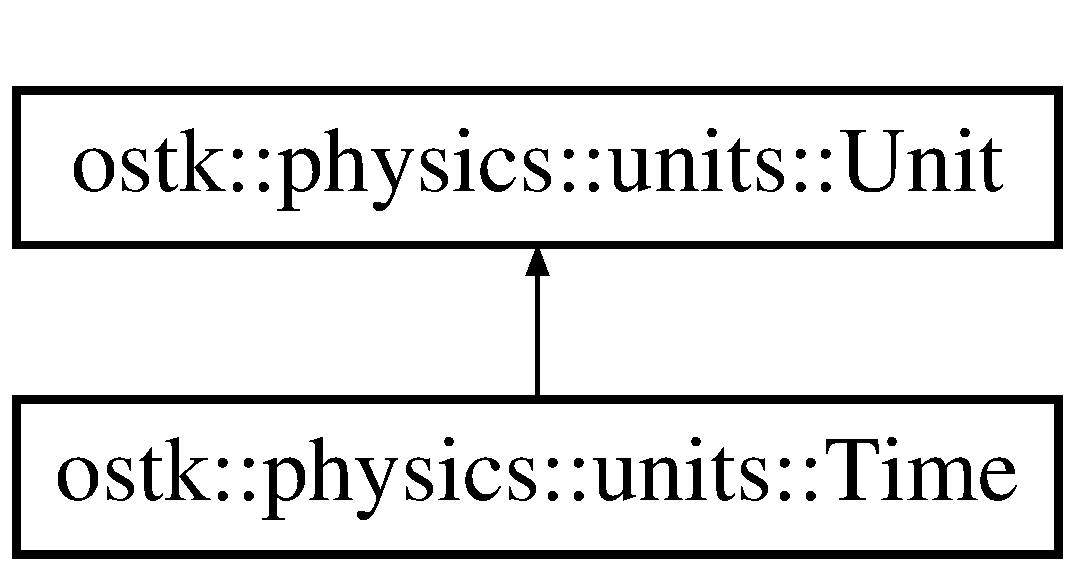
\includegraphics[height=2.000000cm]{classostk_1_1physics_1_1units_1_1_time}
\end{center}
\end{figure}
\subsection*{Public Types}
\begin{DoxyCompactItemize}
\item 
enum \hyperlink{classostk_1_1physics_1_1units_1_1_time_aa961f0dbca7ec297e19e15e0dfa3bb4a}{Unit} \{ \newline
\hyperlink{classostk_1_1physics_1_1units_1_1_time_aa961f0dbca7ec297e19e15e0dfa3bb4aaec0fc0100c4fc1ce4eea230c3dc10360}{Unit\+::\+Undefined}, 
\hyperlink{classostk_1_1physics_1_1units_1_1_time_aa961f0dbca7ec297e19e15e0dfa3bb4aa4146c294bcc82b1723c65bdc64b55089}{Unit\+::\+Nanosecond}, 
\hyperlink{classostk_1_1physics_1_1units_1_1_time_aa961f0dbca7ec297e19e15e0dfa3bb4aa1f14b3811ca5de688daa740d8471249e}{Unit\+::\+Microsecond}, 
\hyperlink{classostk_1_1physics_1_1units_1_1_time_aa961f0dbca7ec297e19e15e0dfa3bb4aa988bbeeb80e7e0a6b4651aab5a76b413}{Unit\+::\+Millisecond}, 
\newline
\hyperlink{classostk_1_1physics_1_1units_1_1_time_aa961f0dbca7ec297e19e15e0dfa3bb4aac22cf8376b1893dcfcef0649fe1a7d87}{Unit\+::\+Second}, 
\hyperlink{classostk_1_1physics_1_1units_1_1_time_aa961f0dbca7ec297e19e15e0dfa3bb4aa62902641c38f3a4a8eb3212454360e24}{Unit\+::\+Minute}, 
\hyperlink{classostk_1_1physics_1_1units_1_1_time_aa961f0dbca7ec297e19e15e0dfa3bb4aab55e509c697e4cca0e1d160a7806698f}{Unit\+::\+Hour}, 
\hyperlink{classostk_1_1physics_1_1units_1_1_time_aa961f0dbca7ec297e19e15e0dfa3bb4aa03727ac48595a24daed975559c944a44}{Unit\+::\+Day}, 
\newline
\hyperlink{classostk_1_1physics_1_1units_1_1_time_aa961f0dbca7ec297e19e15e0dfa3bb4aad2ce009594dcc60befa6a4e6cbeb71fc}{Unit\+::\+Week}
 \}
\end{DoxyCompactItemize}
\subsection*{Public Member Functions}
\begin{DoxyCompactItemize}
\item 
\hyperlink{classostk_1_1physics_1_1units_1_1_time_a731e1f09af9f9e95cac914cc189cbbad}{Time} (const Real \&a\+Value, const \hyperlink{classostk_1_1physics_1_1units_1_1_time_aa961f0dbca7ec297e19e15e0dfa3bb4a}{Time\+::\+Unit} \&a\+Unit)
\begin{DoxyCompactList}\small\item\em Constructor. \end{DoxyCompactList}\item 
virtual \hyperlink{classostk_1_1physics_1_1units_1_1_time}{Time} $\ast$ \hyperlink{classostk_1_1physics_1_1units_1_1_time_ae714d9f44d7ab651de5f37c5085f38fa}{clone} () const override
\item 
virtual bool \hyperlink{classostk_1_1physics_1_1units_1_1_time_a1b89925067e81636fa80f6e73eed3625}{is\+Defined} () const override
\item 
\hyperlink{classostk_1_1physics_1_1units_1_1_time_aa961f0dbca7ec297e19e15e0dfa3bb4a}{Time\+::\+Unit} \hyperlink{classostk_1_1physics_1_1units_1_1_time_a2e6a342d3c8b7ee85764223855056fb0}{get\+Unit} () const
\item 
Real \hyperlink{classostk_1_1physics_1_1units_1_1_time_a222edb0c7de6cfbc5ae29632261bc829}{in} (const \hyperlink{classostk_1_1physics_1_1units_1_1_time_aa961f0dbca7ec297e19e15e0dfa3bb4a}{Time\+::\+Unit} \&a\+Unit) const
\item 
Real \hyperlink{classostk_1_1physics_1_1units_1_1_time_afbb52cb65acea3748fdd1952fc9d81ee}{in\+Seconds} () const
\item 
virtual String \hyperlink{classostk_1_1physics_1_1units_1_1_time_a6805d7d9b298d1ba9f219294e11a363c}{to\+String} (const Integer \&a\+Precision=Integer\+::\+Undefined()) const override
\end{DoxyCompactItemize}
\subsection*{Static Public Member Functions}
\begin{DoxyCompactItemize}
\item 
static \hyperlink{classostk_1_1physics_1_1units_1_1_time}{Time} \hyperlink{classostk_1_1physics_1_1units_1_1_time_a441dc384583635132e8e068425114ca4}{Undefined} ()
\item 
static \hyperlink{classostk_1_1physics_1_1units_1_1_time}{Time} \hyperlink{classostk_1_1physics_1_1units_1_1_time_a033cfbfb3fb4346fd073f3007512b4f6}{Seconds} (const Real \&a\+Value)
\item 
static String \hyperlink{classostk_1_1physics_1_1units_1_1_time_a598f5cb08cf2e7b5851322c1c0a31044}{String\+From\+Unit} (const \hyperlink{classostk_1_1physics_1_1units_1_1_time_aa961f0dbca7ec297e19e15e0dfa3bb4a}{Time\+::\+Unit} \&a\+Unit)
\item 
static String \hyperlink{classostk_1_1physics_1_1units_1_1_time_ae9740ed97b634fb099d1ba46e064cb0c}{Symbol\+From\+Unit} (const \hyperlink{classostk_1_1physics_1_1units_1_1_time_aa961f0dbca7ec297e19e15e0dfa3bb4a}{Time\+::\+Unit} \&a\+Unit)
\end{DoxyCompactItemize}
\subsection*{Additional Inherited Members}


\subsection{Detailed Description}
\hyperlink{classostk_1_1physics_1_1units_1_1_time}{Time}. 

https\+://en.wikipedia.\+org/wiki/\+Unit\+\_\+of\+\_\+time 

\subsection{Member Enumeration Documentation}
\mbox{\Hypertarget{classostk_1_1physics_1_1units_1_1_time_aa961f0dbca7ec297e19e15e0dfa3bb4a}\label{classostk_1_1physics_1_1units_1_1_time_aa961f0dbca7ec297e19e15e0dfa3bb4a}} 
\index{ostk\+::physics\+::units\+::\+Time@{ostk\+::physics\+::units\+::\+Time}!Unit@{Unit}}
\index{Unit@{Unit}!ostk\+::physics\+::units\+::\+Time@{ostk\+::physics\+::units\+::\+Time}}
\subsubsection{\texorpdfstring{Unit}{Unit}}
{\footnotesize\ttfamily enum \hyperlink{classostk_1_1physics_1_1units_1_1_time_aa961f0dbca7ec297e19e15e0dfa3bb4a}{ostk\+::physics\+::units\+::\+Time\+::\+Unit}\hspace{0.3cm}{\ttfamily [strong]}}

\begin{DoxyEnumFields}{Enumerator}
\raisebox{\heightof{T}}[0pt][0pt]{\index{Undefined@{Undefined}!ostk\+::physics\+::units\+::\+Time@{ostk\+::physics\+::units\+::\+Time}}\index{ostk\+::physics\+::units\+::\+Time@{ostk\+::physics\+::units\+::\+Time}!Undefined@{Undefined}}}\mbox{\Hypertarget{classostk_1_1physics_1_1units_1_1_time_aa961f0dbca7ec297e19e15e0dfa3bb4aaec0fc0100c4fc1ce4eea230c3dc10360}\label{classostk_1_1physics_1_1units_1_1_time_aa961f0dbca7ec297e19e15e0dfa3bb4aaec0fc0100c4fc1ce4eea230c3dc10360}} 
Undefined&Undefined. \\
\hline

\raisebox{\heightof{T}}[0pt][0pt]{\index{Nanosecond@{Nanosecond}!ostk\+::physics\+::units\+::\+Time@{ostk\+::physics\+::units\+::\+Time}}\index{ostk\+::physics\+::units\+::\+Time@{ostk\+::physics\+::units\+::\+Time}!Nanosecond@{Nanosecond}}}\mbox{\Hypertarget{classostk_1_1physics_1_1units_1_1_time_aa961f0dbca7ec297e19e15e0dfa3bb4aa4146c294bcc82b1723c65bdc64b55089}\label{classostk_1_1physics_1_1units_1_1_time_aa961f0dbca7ec297e19e15e0dfa3bb4aa4146c294bcc82b1723c65bdc64b55089}} 
Nanosecond&Nanosecond. \\
\hline

\raisebox{\heightof{T}}[0pt][0pt]{\index{Microsecond@{Microsecond}!ostk\+::physics\+::units\+::\+Time@{ostk\+::physics\+::units\+::\+Time}}\index{ostk\+::physics\+::units\+::\+Time@{ostk\+::physics\+::units\+::\+Time}!Microsecond@{Microsecond}}}\mbox{\Hypertarget{classostk_1_1physics_1_1units_1_1_time_aa961f0dbca7ec297e19e15e0dfa3bb4aa1f14b3811ca5de688daa740d8471249e}\label{classostk_1_1physics_1_1units_1_1_time_aa961f0dbca7ec297e19e15e0dfa3bb4aa1f14b3811ca5de688daa740d8471249e}} 
Microsecond&Microsecond. \\
\hline

\raisebox{\heightof{T}}[0pt][0pt]{\index{Millisecond@{Millisecond}!ostk\+::physics\+::units\+::\+Time@{ostk\+::physics\+::units\+::\+Time}}\index{ostk\+::physics\+::units\+::\+Time@{ostk\+::physics\+::units\+::\+Time}!Millisecond@{Millisecond}}}\mbox{\Hypertarget{classostk_1_1physics_1_1units_1_1_time_aa961f0dbca7ec297e19e15e0dfa3bb4aa988bbeeb80e7e0a6b4651aab5a76b413}\label{classostk_1_1physics_1_1units_1_1_time_aa961f0dbca7ec297e19e15e0dfa3bb4aa988bbeeb80e7e0a6b4651aab5a76b413}} 
Millisecond&Millisecond. \\
\hline

\raisebox{\heightof{T}}[0pt][0pt]{\index{Second@{Second}!ostk\+::physics\+::units\+::\+Time@{ostk\+::physics\+::units\+::\+Time}}\index{ostk\+::physics\+::units\+::\+Time@{ostk\+::physics\+::units\+::\+Time}!Second@{Second}}}\mbox{\Hypertarget{classostk_1_1physics_1_1units_1_1_time_aa961f0dbca7ec297e19e15e0dfa3bb4aac22cf8376b1893dcfcef0649fe1a7d87}\label{classostk_1_1physics_1_1units_1_1_time_aa961f0dbca7ec297e19e15e0dfa3bb4aac22cf8376b1893dcfcef0649fe1a7d87}} 
Second&Second (SI) \\
\hline

\raisebox{\heightof{T}}[0pt][0pt]{\index{Minute@{Minute}!ostk\+::physics\+::units\+::\+Time@{ostk\+::physics\+::units\+::\+Time}}\index{ostk\+::physics\+::units\+::\+Time@{ostk\+::physics\+::units\+::\+Time}!Minute@{Minute}}}\mbox{\Hypertarget{classostk_1_1physics_1_1units_1_1_time_aa961f0dbca7ec297e19e15e0dfa3bb4aa62902641c38f3a4a8eb3212454360e24}\label{classostk_1_1physics_1_1units_1_1_time_aa961f0dbca7ec297e19e15e0dfa3bb4aa62902641c38f3a4a8eb3212454360e24}} 
Minute&Minute. \\
\hline

\raisebox{\heightof{T}}[0pt][0pt]{\index{Hour@{Hour}!ostk\+::physics\+::units\+::\+Time@{ostk\+::physics\+::units\+::\+Time}}\index{ostk\+::physics\+::units\+::\+Time@{ostk\+::physics\+::units\+::\+Time}!Hour@{Hour}}}\mbox{\Hypertarget{classostk_1_1physics_1_1units_1_1_time_aa961f0dbca7ec297e19e15e0dfa3bb4aab55e509c697e4cca0e1d160a7806698f}\label{classostk_1_1physics_1_1units_1_1_time_aa961f0dbca7ec297e19e15e0dfa3bb4aab55e509c697e4cca0e1d160a7806698f}} 
Hour&Hour. \\
\hline

\raisebox{\heightof{T}}[0pt][0pt]{\index{Day@{Day}!ostk\+::physics\+::units\+::\+Time@{ostk\+::physics\+::units\+::\+Time}}\index{ostk\+::physics\+::units\+::\+Time@{ostk\+::physics\+::units\+::\+Time}!Day@{Day}}}\mbox{\Hypertarget{classostk_1_1physics_1_1units_1_1_time_aa961f0dbca7ec297e19e15e0dfa3bb4aa03727ac48595a24daed975559c944a44}\label{classostk_1_1physics_1_1units_1_1_time_aa961f0dbca7ec297e19e15e0dfa3bb4aa03727ac48595a24daed975559c944a44}} 
Day&Day. \\
\hline

\raisebox{\heightof{T}}[0pt][0pt]{\index{Week@{Week}!ostk\+::physics\+::units\+::\+Time@{ostk\+::physics\+::units\+::\+Time}}\index{ostk\+::physics\+::units\+::\+Time@{ostk\+::physics\+::units\+::\+Time}!Week@{Week}}}\mbox{\Hypertarget{classostk_1_1physics_1_1units_1_1_time_aa961f0dbca7ec297e19e15e0dfa3bb4aad2ce009594dcc60befa6a4e6cbeb71fc}\label{classostk_1_1physics_1_1units_1_1_time_aa961f0dbca7ec297e19e15e0dfa3bb4aad2ce009594dcc60befa6a4e6cbeb71fc}} 
Week&Week. \\
\hline

\end{DoxyEnumFields}


\subsection{Constructor \& Destructor Documentation}
\mbox{\Hypertarget{classostk_1_1physics_1_1units_1_1_time_a731e1f09af9f9e95cac914cc189cbbad}\label{classostk_1_1physics_1_1units_1_1_time_a731e1f09af9f9e95cac914cc189cbbad}} 
\index{ostk\+::physics\+::units\+::\+Time@{ostk\+::physics\+::units\+::\+Time}!Time@{Time}}
\index{Time@{Time}!ostk\+::physics\+::units\+::\+Time@{ostk\+::physics\+::units\+::\+Time}}
\subsubsection{\texorpdfstring{Time()}{Time()}}
{\footnotesize\ttfamily ostk\+::physics\+::units\+::\+Time\+::\+Time (\begin{DoxyParamCaption}\item[{const Real \&}]{a\+Value,  }\item[{const \hyperlink{classostk_1_1physics_1_1units_1_1_time_aa961f0dbca7ec297e19e15e0dfa3bb4a}{Time\+::\+Unit} \&}]{a\+Unit }\end{DoxyParamCaption})}



Constructor. 


\begin{DoxyCode}
\hyperlink{classostk_1_1physics_1_1units_1_1_time_a731e1f09af9f9e95cac914cc189cbbad}{Time} time(1.0, \hyperlink{classostk_1_1physics_1_1units_1_1_time_aa961f0dbca7ec297e19e15e0dfa3bb4aac22cf8376b1893dcfcef0649fe1a7d87}{Time::Unit::Second}) ;
\end{DoxyCode}



\begin{DoxyParams}[1]{Parameters}
\mbox{\tt in}  & {\em a\+Value} & A value \\
\hline
\mbox{\tt in}  & {\em a\+Unit} & A time unit \\
\hline
\end{DoxyParams}


\subsection{Member Function Documentation}
\mbox{\Hypertarget{classostk_1_1physics_1_1units_1_1_time_ae714d9f44d7ab651de5f37c5085f38fa}\label{classostk_1_1physics_1_1units_1_1_time_ae714d9f44d7ab651de5f37c5085f38fa}} 
\index{ostk\+::physics\+::units\+::\+Time@{ostk\+::physics\+::units\+::\+Time}!clone@{clone}}
\index{clone@{clone}!ostk\+::physics\+::units\+::\+Time@{ostk\+::physics\+::units\+::\+Time}}
\subsubsection{\texorpdfstring{clone()}{clone()}}
{\footnotesize\ttfamily \hyperlink{classostk_1_1physics_1_1units_1_1_time}{Time} $\ast$ ostk\+::physics\+::units\+::\+Time\+::clone (\begin{DoxyParamCaption}{ }\end{DoxyParamCaption}) const\hspace{0.3cm}{\ttfamily [override]}, {\ttfamily [virtual]}}



Implements \hyperlink{classostk_1_1physics_1_1units_1_1_unit_ab203628f8a16b16c28d89eaa4c3aff67}{ostk\+::physics\+::units\+::\+Unit}.

\mbox{\Hypertarget{classostk_1_1physics_1_1units_1_1_time_a2e6a342d3c8b7ee85764223855056fb0}\label{classostk_1_1physics_1_1units_1_1_time_a2e6a342d3c8b7ee85764223855056fb0}} 
\index{ostk\+::physics\+::units\+::\+Time@{ostk\+::physics\+::units\+::\+Time}!get\+Unit@{get\+Unit}}
\index{get\+Unit@{get\+Unit}!ostk\+::physics\+::units\+::\+Time@{ostk\+::physics\+::units\+::\+Time}}
\subsubsection{\texorpdfstring{get\+Unit()}{getUnit()}}
{\footnotesize\ttfamily \hyperlink{classostk_1_1physics_1_1units_1_1_time_aa961f0dbca7ec297e19e15e0dfa3bb4a}{Time\+::\+Unit} ostk\+::physics\+::units\+::\+Time\+::get\+Unit (\begin{DoxyParamCaption}{ }\end{DoxyParamCaption}) const}

\mbox{\Hypertarget{classostk_1_1physics_1_1units_1_1_time_a222edb0c7de6cfbc5ae29632261bc829}\label{classostk_1_1physics_1_1units_1_1_time_a222edb0c7de6cfbc5ae29632261bc829}} 
\index{ostk\+::physics\+::units\+::\+Time@{ostk\+::physics\+::units\+::\+Time}!in@{in}}
\index{in@{in}!ostk\+::physics\+::units\+::\+Time@{ostk\+::physics\+::units\+::\+Time}}
\subsubsection{\texorpdfstring{in()}{in()}}
{\footnotesize\ttfamily Real ostk\+::physics\+::units\+::\+Time\+::in (\begin{DoxyParamCaption}\item[{const \hyperlink{classostk_1_1physics_1_1units_1_1_time_aa961f0dbca7ec297e19e15e0dfa3bb4a}{Time\+::\+Unit} \&}]{a\+Unit }\end{DoxyParamCaption}) const}

\mbox{\Hypertarget{classostk_1_1physics_1_1units_1_1_time_afbb52cb65acea3748fdd1952fc9d81ee}\label{classostk_1_1physics_1_1units_1_1_time_afbb52cb65acea3748fdd1952fc9d81ee}} 
\index{ostk\+::physics\+::units\+::\+Time@{ostk\+::physics\+::units\+::\+Time}!in\+Seconds@{in\+Seconds}}
\index{in\+Seconds@{in\+Seconds}!ostk\+::physics\+::units\+::\+Time@{ostk\+::physics\+::units\+::\+Time}}
\subsubsection{\texorpdfstring{in\+Seconds()}{inSeconds()}}
{\footnotesize\ttfamily Real ostk\+::physics\+::units\+::\+Time\+::in\+Seconds (\begin{DoxyParamCaption}{ }\end{DoxyParamCaption}) const}

\mbox{\Hypertarget{classostk_1_1physics_1_1units_1_1_time_a1b89925067e81636fa80f6e73eed3625}\label{classostk_1_1physics_1_1units_1_1_time_a1b89925067e81636fa80f6e73eed3625}} 
\index{ostk\+::physics\+::units\+::\+Time@{ostk\+::physics\+::units\+::\+Time}!is\+Defined@{is\+Defined}}
\index{is\+Defined@{is\+Defined}!ostk\+::physics\+::units\+::\+Time@{ostk\+::physics\+::units\+::\+Time}}
\subsubsection{\texorpdfstring{is\+Defined()}{isDefined()}}
{\footnotesize\ttfamily bool ostk\+::physics\+::units\+::\+Time\+::is\+Defined (\begin{DoxyParamCaption}{ }\end{DoxyParamCaption}) const\hspace{0.3cm}{\ttfamily [override]}, {\ttfamily [virtual]}}



Reimplemented from \hyperlink{classostk_1_1physics_1_1units_1_1_unit_a423ce1df3478f0892b10824b591ae1cc}{ostk\+::physics\+::units\+::\+Unit}.

\mbox{\Hypertarget{classostk_1_1physics_1_1units_1_1_time_a033cfbfb3fb4346fd073f3007512b4f6}\label{classostk_1_1physics_1_1units_1_1_time_a033cfbfb3fb4346fd073f3007512b4f6}} 
\index{ostk\+::physics\+::units\+::\+Time@{ostk\+::physics\+::units\+::\+Time}!Seconds@{Seconds}}
\index{Seconds@{Seconds}!ostk\+::physics\+::units\+::\+Time@{ostk\+::physics\+::units\+::\+Time}}
\subsubsection{\texorpdfstring{Seconds()}{Seconds()}}
{\footnotesize\ttfamily \hyperlink{classostk_1_1physics_1_1units_1_1_time}{Time} ostk\+::physics\+::units\+::\+Time\+::\+Seconds (\begin{DoxyParamCaption}\item[{const Real \&}]{a\+Value }\end{DoxyParamCaption})\hspace{0.3cm}{\ttfamily [static]}}

\mbox{\Hypertarget{classostk_1_1physics_1_1units_1_1_time_a598f5cb08cf2e7b5851322c1c0a31044}\label{classostk_1_1physics_1_1units_1_1_time_a598f5cb08cf2e7b5851322c1c0a31044}} 
\index{ostk\+::physics\+::units\+::\+Time@{ostk\+::physics\+::units\+::\+Time}!String\+From\+Unit@{String\+From\+Unit}}
\index{String\+From\+Unit@{String\+From\+Unit}!ostk\+::physics\+::units\+::\+Time@{ostk\+::physics\+::units\+::\+Time}}
\subsubsection{\texorpdfstring{String\+From\+Unit()}{StringFromUnit()}}
{\footnotesize\ttfamily String ostk\+::physics\+::units\+::\+Time\+::\+String\+From\+Unit (\begin{DoxyParamCaption}\item[{const \hyperlink{classostk_1_1physics_1_1units_1_1_time_aa961f0dbca7ec297e19e15e0dfa3bb4a}{Time\+::\+Unit} \&}]{a\+Unit }\end{DoxyParamCaption})\hspace{0.3cm}{\ttfamily [static]}}

\mbox{\Hypertarget{classostk_1_1physics_1_1units_1_1_time_ae9740ed97b634fb099d1ba46e064cb0c}\label{classostk_1_1physics_1_1units_1_1_time_ae9740ed97b634fb099d1ba46e064cb0c}} 
\index{ostk\+::physics\+::units\+::\+Time@{ostk\+::physics\+::units\+::\+Time}!Symbol\+From\+Unit@{Symbol\+From\+Unit}}
\index{Symbol\+From\+Unit@{Symbol\+From\+Unit}!ostk\+::physics\+::units\+::\+Time@{ostk\+::physics\+::units\+::\+Time}}
\subsubsection{\texorpdfstring{Symbol\+From\+Unit()}{SymbolFromUnit()}}
{\footnotesize\ttfamily String ostk\+::physics\+::units\+::\+Time\+::\+Symbol\+From\+Unit (\begin{DoxyParamCaption}\item[{const \hyperlink{classostk_1_1physics_1_1units_1_1_time_aa961f0dbca7ec297e19e15e0dfa3bb4a}{Time\+::\+Unit} \&}]{a\+Unit }\end{DoxyParamCaption})\hspace{0.3cm}{\ttfamily [static]}}

\mbox{\Hypertarget{classostk_1_1physics_1_1units_1_1_time_a6805d7d9b298d1ba9f219294e11a363c}\label{classostk_1_1physics_1_1units_1_1_time_a6805d7d9b298d1ba9f219294e11a363c}} 
\index{ostk\+::physics\+::units\+::\+Time@{ostk\+::physics\+::units\+::\+Time}!to\+String@{to\+String}}
\index{to\+String@{to\+String}!ostk\+::physics\+::units\+::\+Time@{ostk\+::physics\+::units\+::\+Time}}
\subsubsection{\texorpdfstring{to\+String()}{toString()}}
{\footnotesize\ttfamily String ostk\+::physics\+::units\+::\+Time\+::to\+String (\begin{DoxyParamCaption}\item[{const Integer \&}]{a\+Precision = {\ttfamily Integer\+:\+:Undefined()} }\end{DoxyParamCaption}) const\hspace{0.3cm}{\ttfamily [override]}, {\ttfamily [virtual]}}



Implements \hyperlink{classostk_1_1physics_1_1units_1_1_unit_a8162b4eb8221c7577af16ab8b399d07e}{ostk\+::physics\+::units\+::\+Unit}.

\mbox{\Hypertarget{classostk_1_1physics_1_1units_1_1_time_a441dc384583635132e8e068425114ca4}\label{classostk_1_1physics_1_1units_1_1_time_a441dc384583635132e8e068425114ca4}} 
\index{ostk\+::physics\+::units\+::\+Time@{ostk\+::physics\+::units\+::\+Time}!Undefined@{Undefined}}
\index{Undefined@{Undefined}!ostk\+::physics\+::units\+::\+Time@{ostk\+::physics\+::units\+::\+Time}}
\subsubsection{\texorpdfstring{Undefined()}{Undefined()}}
{\footnotesize\ttfamily \hyperlink{classostk_1_1physics_1_1units_1_1_time}{Time} ostk\+::physics\+::units\+::\+Time\+::\+Undefined (\begin{DoxyParamCaption}{ }\end{DoxyParamCaption})\hspace{0.3cm}{\ttfamily [static]}}



The documentation for this class was generated from the following files\+:\begin{DoxyCompactItemize}
\item 
include/\+Open\+Space\+Toolkit/\+Physics/\+Units/\hyperlink{_units_2_time_8hpp}{Time.\+hpp}\item 
src/\+Open\+Space\+Toolkit/\+Physics/\+Units/\hyperlink{_units_2_time_8cpp}{Time.\+cpp}\end{DoxyCompactItemize}

\hypertarget{classostk_1_1physics_1_1time_1_1_time}{}\section{ostk\+:\+:physics\+:\+:time\+:\+:Time Class Reference}
\label{classostk_1_1physics_1_1time_1_1_time}\index{ostk\+::physics\+::time\+::\+Time@{ostk\+::physics\+::time\+::\+Time}}


\hyperlink{classostk_1_1physics_1_1time_1_1_time}{Time} as hour, minute, second, millisecond, microsecond and nanosecond.  




{\ttfamily \#include $<$Time.\+hpp$>$}

\subsection*{Public Types}
\begin{DoxyCompactItemize}
\item 
enum \hyperlink{classostk_1_1physics_1_1time_1_1_time_a207e776746c45c3aaffcf7112b2bc951}{Format} \{ \hyperlink{classostk_1_1physics_1_1time_1_1_time_a207e776746c45c3aaffcf7112b2bc951aec0fc0100c4fc1ce4eea230c3dc10360}{Format\+::\+Undefined}, 
\hyperlink{classostk_1_1physics_1_1time_1_1_time_a207e776746c45c3aaffcf7112b2bc951aeb6d8ae6f20283755b339c0dc273988b}{Format\+::\+Standard}, 
\hyperlink{classostk_1_1physics_1_1time_1_1_time_a207e776746c45c3aaffcf7112b2bc951a35b6786739efcdc5a74ab1dca29d3b6b}{Format\+::\+I\+S\+O8601}
 \}\begin{DoxyCompactList}\small\item\em \hyperlink{classostk_1_1physics_1_1time_1_1_time}{Time} format. \end{DoxyCompactList}
\end{DoxyCompactItemize}
\subsection*{Public Member Functions}
\begin{DoxyCompactItemize}
\item 
\hyperlink{classostk_1_1physics_1_1time_1_1_time_a9609e75d328ed240f6fc4529e26038cc}{Time} (Uint8 an\+Hour, Uint8 a\+Minute, Uint8 a\+Second, Uint16 a\+Millisecond=0, Uint16 a\+Microsecond=0, Uint16 a\+Nanosecond=0)
\begin{DoxyCompactList}\small\item\em Constructor. \end{DoxyCompactList}\item 
bool \hyperlink{classostk_1_1physics_1_1time_1_1_time_ad914e61c2ace9527236f88b897a0c6de}{operator==} (const \hyperlink{classostk_1_1physics_1_1time_1_1_time}{Time} \&a\+Time) const
\begin{DoxyCompactList}\small\item\em Equal to operator. \end{DoxyCompactList}\item 
bool \hyperlink{classostk_1_1physics_1_1time_1_1_time_a0e33fd17972bc71d52b159559f8180c8}{operator!=} (const \hyperlink{classostk_1_1physics_1_1time_1_1_time}{Time} \&a\+Time) const
\begin{DoxyCompactList}\small\item\em Not equal to operator. \end{DoxyCompactList}\item 
bool \hyperlink{classostk_1_1physics_1_1time_1_1_time_a25f4b6019bc558ca579aca4af8aa1ec0}{is\+Defined} () const
\begin{DoxyCompactList}\small\item\em Check if time is defined. \end{DoxyCompactList}\item 
Uint8 \hyperlink{classostk_1_1physics_1_1time_1_1_time_adc56fbb417453265e6d5a448e597fd76}{get\+Hour} () const
\begin{DoxyCompactList}\small\item\em Get hour (0 -\/ 23) \end{DoxyCompactList}\item 
Uint8 \hyperlink{classostk_1_1physics_1_1time_1_1_time_a19ccd8123a0d3e24b90bd1dc964d40ce}{get\+Minute} () const
\begin{DoxyCompactList}\small\item\em Get minute (0 -\/ 59) \end{DoxyCompactList}\item 
Uint8 \hyperlink{classostk_1_1physics_1_1time_1_1_time_afe4041426b008059853110b13e2802de}{get\+Second} () const
\begin{DoxyCompactList}\small\item\em Get second (0 -\/ 60) \end{DoxyCompactList}\item 
Uint16 \hyperlink{classostk_1_1physics_1_1time_1_1_time_a73308a0a9dcf7105130d1b40d2ef7d93}{get\+Millisecond} () const
\begin{DoxyCompactList}\small\item\em Get millisecond (0 -\/ 999) \end{DoxyCompactList}\item 
Uint16 \hyperlink{classostk_1_1physics_1_1time_1_1_time_acb4915ca99f2065f6d777d96833337db}{get\+Microsecond} () const
\begin{DoxyCompactList}\small\item\em Get microsecond (0 -\/ 999) \end{DoxyCompactList}\item 
Uint16 \hyperlink{classostk_1_1physics_1_1time_1_1_time_aebe3fc329d7b7b07c1f0ac04600ebc03}{get\+Nanosecond} () const
\begin{DoxyCompactList}\small\item\em Get nanosecond (0 -\/ 999) \end{DoxyCompactList}\item 
Real \hyperlink{classostk_1_1physics_1_1time_1_1_time_ad0c70220f4ba971306781eb92d8f2030}{get\+Floating\+Seconds} () const
\begin{DoxyCompactList}\small\item\em Get floating seconds (0.\+0 -\/ 59.\+999999999) \end{DoxyCompactList}\item 
String \hyperlink{classostk_1_1physics_1_1time_1_1_time_a33adb26e33abdfa65581626372f430bd}{to\+String} (const \hyperlink{classostk_1_1physics_1_1time_1_1_time_a207e776746c45c3aaffcf7112b2bc951}{Time\+::\+Format} \&a\+Format=\hyperlink{classostk_1_1physics_1_1time_1_1_time_a207e776746c45c3aaffcf7112b2bc951aeb6d8ae6f20283755b339c0dc273988b}{Time\+::\+Format\+::\+Standard}) const
\begin{DoxyCompactList}\small\item\em Get string representation of time. \end{DoxyCompactList}\item 
void \hyperlink{classostk_1_1physics_1_1time_1_1_time_a27d456d374f5799050f3ea8aed8478ac}{set\+Hour} (Uint8 an\+Hour)
\begin{DoxyCompactList}\small\item\em Set hour. \end{DoxyCompactList}\item 
void \hyperlink{classostk_1_1physics_1_1time_1_1_time_aef028b25ce2ff2d216e9fdc957c6ac4f}{set\+Minute} (Uint8 a\+Minute)
\begin{DoxyCompactList}\small\item\em Set minute. \end{DoxyCompactList}\item 
void \hyperlink{classostk_1_1physics_1_1time_1_1_time_a4f5cc2bb2a6ff653eca82e5a754fa781}{set\+Second} (Uint8 a\+Second)
\begin{DoxyCompactList}\small\item\em Set second. \end{DoxyCompactList}\item 
void \hyperlink{classostk_1_1physics_1_1time_1_1_time_a78a51113cfca7af8e14fbf519b04ad25}{set\+Millisecond} (Uint16 a\+Millisecond)
\begin{DoxyCompactList}\small\item\em Set millisecond. \end{DoxyCompactList}\item 
void \hyperlink{classostk_1_1physics_1_1time_1_1_time_a4e746282febe29d5412f7e871b49ac86}{set\+Microsecond} (Uint16 a\+Microsecond)
\begin{DoxyCompactList}\small\item\em Set microsecond. \end{DoxyCompactList}\item 
void \hyperlink{classostk_1_1physics_1_1time_1_1_time_a35df10195d96fe03990493a52cd7d61e}{set\+Nanosecond} (Uint16 a\+Nanosecond)
\begin{DoxyCompactList}\small\item\em Set nanosecond. \end{DoxyCompactList}\end{DoxyCompactItemize}
\subsection*{Static Public Member Functions}
\begin{DoxyCompactItemize}
\item 
static \hyperlink{classostk_1_1physics_1_1time_1_1_time}{Time} \hyperlink{classostk_1_1physics_1_1time_1_1_time_a17c9ae2f4fa9c8a48a558fa49c511e03}{Undefined} ()
\begin{DoxyCompactList}\small\item\em Constructs an undefined time. \end{DoxyCompactList}\item 
static \hyperlink{classostk_1_1physics_1_1time_1_1_time}{Time} \hyperlink{classostk_1_1physics_1_1time_1_1_time_a74042a99c99ef0f866204a4589c6a89e}{Midnight} ()
\begin{DoxyCompactList}\small\item\em Constructs a time at midnight. \end{DoxyCompactList}\item 
static \hyperlink{classostk_1_1physics_1_1time_1_1_time}{Time} \hyperlink{classostk_1_1physics_1_1time_1_1_time_a2d242e4f07bbf56e51eb2267773042f2}{Noon} ()
\begin{DoxyCompactList}\small\item\em Constructs a time at noon. \end{DoxyCompactList}\item 
static \hyperlink{classostk_1_1physics_1_1time_1_1_time}{Time} \hyperlink{classostk_1_1physics_1_1time_1_1_time_a475b2b6200f15f20c8fab3891bbb73ac}{Parse} (const String \&a\+String, const \hyperlink{classostk_1_1physics_1_1time_1_1_time_a207e776746c45c3aaffcf7112b2bc951}{Time\+::\+Format} \&a\+Format=\hyperlink{classostk_1_1physics_1_1time_1_1_time_a207e776746c45c3aaffcf7112b2bc951aec0fc0100c4fc1ce4eea230c3dc10360}{Time\+::\+Format\+::\+Undefined})
\begin{DoxyCompactList}\small\item\em Constructs a time from a string representation. \end{DoxyCompactList}\end{DoxyCompactItemize}
\subsection*{Friends}
\begin{DoxyCompactItemize}
\item 
std\+::ostream \& \hyperlink{classostk_1_1physics_1_1time_1_1_time_a181948621d8fe0d85bdfc97af30b62fb}{operator$<$$<$} (std\+::ostream \&an\+Output\+Stream, const \hyperlink{classostk_1_1physics_1_1time_1_1_time}{Time} \&a\+Time)
\begin{DoxyCompactList}\small\item\em Output stream operator. \end{DoxyCompactList}\end{DoxyCompactItemize}


\subsection{Detailed Description}
\hyperlink{classostk_1_1physics_1_1time_1_1_time}{Time} as hour, minute, second, millisecond, microsecond and nanosecond. 

\subsection{Member Enumeration Documentation}
\mbox{\Hypertarget{classostk_1_1physics_1_1time_1_1_time_a207e776746c45c3aaffcf7112b2bc951}\label{classostk_1_1physics_1_1time_1_1_time_a207e776746c45c3aaffcf7112b2bc951}} 
\index{ostk\+::physics\+::time\+::\+Time@{ostk\+::physics\+::time\+::\+Time}!Format@{Format}}
\index{Format@{Format}!ostk\+::physics\+::time\+::\+Time@{ostk\+::physics\+::time\+::\+Time}}
\subsubsection{\texorpdfstring{Format}{Format}}
{\footnotesize\ttfamily enum \hyperlink{classostk_1_1physics_1_1time_1_1_time_a207e776746c45c3aaffcf7112b2bc951}{ostk\+::physics\+::time\+::\+Time\+::\+Format}\hspace{0.3cm}{\ttfamily [strong]}}



\hyperlink{classostk_1_1physics_1_1time_1_1_time}{Time} format. 

\begin{DoxyEnumFields}{Enumerator}
\raisebox{\heightof{T}}[0pt][0pt]{\index{Undefined@{Undefined}!ostk\+::physics\+::time\+::\+Time@{ostk\+::physics\+::time\+::\+Time}}\index{ostk\+::physics\+::time\+::\+Time@{ostk\+::physics\+::time\+::\+Time}!Undefined@{Undefined}}}\mbox{\Hypertarget{classostk_1_1physics_1_1time_1_1_time_a207e776746c45c3aaffcf7112b2bc951aec0fc0100c4fc1ce4eea230c3dc10360}\label{classostk_1_1physics_1_1time_1_1_time_a207e776746c45c3aaffcf7112b2bc951aec0fc0100c4fc1ce4eea230c3dc10360}} 
Undefined&Undefined format. \\
\hline

\raisebox{\heightof{T}}[0pt][0pt]{\index{Standard@{Standard}!ostk\+::physics\+::time\+::\+Time@{ostk\+::physics\+::time\+::\+Time}}\index{ostk\+::physics\+::time\+::\+Time@{ostk\+::physics\+::time\+::\+Time}!Standard@{Standard}}}\mbox{\Hypertarget{classostk_1_1physics_1_1time_1_1_time_a207e776746c45c3aaffcf7112b2bc951aeb6d8ae6f20283755b339c0dc273988b}\label{classostk_1_1physics_1_1time_1_1_time_a207e776746c45c3aaffcf7112b2bc951aeb6d8ae6f20283755b339c0dc273988b}} 
Standard&Standard format (hh\+:mm\+:ss.\+sss.\+sss.\+sss) \\
\hline

\raisebox{\heightof{T}}[0pt][0pt]{\index{I\+S\+O8601@{I\+S\+O8601}!ostk\+::physics\+::time\+::\+Time@{ostk\+::physics\+::time\+::\+Time}}\index{ostk\+::physics\+::time\+::\+Time@{ostk\+::physics\+::time\+::\+Time}!I\+S\+O8601@{I\+S\+O8601}}}\mbox{\Hypertarget{classostk_1_1physics_1_1time_1_1_time_a207e776746c45c3aaffcf7112b2bc951a35b6786739efcdc5a74ab1dca29d3b6b}\label{classostk_1_1physics_1_1time_1_1_time_a207e776746c45c3aaffcf7112b2bc951a35b6786739efcdc5a74ab1dca29d3b6b}} 
I\+S\+O8601&I\+SO 8601 format (hh\+:mm\+:ss.\+sssssssss) \\
\hline

\end{DoxyEnumFields}


\subsection{Constructor \& Destructor Documentation}
\mbox{\Hypertarget{classostk_1_1physics_1_1time_1_1_time_a9609e75d328ed240f6fc4529e26038cc}\label{classostk_1_1physics_1_1time_1_1_time_a9609e75d328ed240f6fc4529e26038cc}} 
\index{ostk\+::physics\+::time\+::\+Time@{ostk\+::physics\+::time\+::\+Time}!Time@{Time}}
\index{Time@{Time}!ostk\+::physics\+::time\+::\+Time@{ostk\+::physics\+::time\+::\+Time}}
\subsubsection{\texorpdfstring{Time()}{Time()}}
{\footnotesize\ttfamily ostk\+::physics\+::time\+::\+Time\+::\+Time (\begin{DoxyParamCaption}\item[{Uint8}]{an\+Hour,  }\item[{Uint8}]{a\+Minute,  }\item[{Uint8}]{a\+Second,  }\item[{Uint16}]{a\+Millisecond = {\ttfamily 0},  }\item[{Uint16}]{a\+Microsecond = {\ttfamily 0},  }\item[{Uint16}]{a\+Nanosecond = {\ttfamily 0} }\end{DoxyParamCaption})}



Constructor. 


\begin{DoxyCode}
\hyperlink{classostk_1_1physics_1_1time_1_1_time_a9609e75d328ed240f6fc4529e26038cc}{Time} time \{ 12, 34, 56 \} ; \textcolor{comment}{// 12:34:56.000.000.000}
\hyperlink{classostk_1_1physics_1_1time_1_1_time_a9609e75d328ed240f6fc4529e26038cc}{Time} time \{ 12, 34, 56, 123, 456, 789 \} ; \textcolor{comment}{// 12:34:56.123.456.789}
\end{DoxyCode}



\begin{DoxyParams}[1]{Parameters}
\mbox{\tt in}  & {\em an\+Hour} & An hour count (0 -\/ 23) \\
\hline
\mbox{\tt in}  & {\em a\+Minute} & A minute count (0 -\/ 59) \\
\hline
\mbox{\tt in}  & {\em a\+Second} & A second count (0 -\/ 60) \\
\hline
\mbox{\tt in}  & {\em (optional)} & a\+Millisecond A millisecond count (0 -\/ 999) \\
\hline
\mbox{\tt in}  & {\em (optional)} & a\+Microsecond A microsecond count (0 -\/ 999) \\
\hline
\mbox{\tt in}  & {\em (optional)} & a\+Nanosecond A nanosecond count (0 -\/ 999) \\
\hline
\end{DoxyParams}


\subsection{Member Function Documentation}
\mbox{\Hypertarget{classostk_1_1physics_1_1time_1_1_time_ad0c70220f4ba971306781eb92d8f2030}\label{classostk_1_1physics_1_1time_1_1_time_ad0c70220f4ba971306781eb92d8f2030}} 
\index{ostk\+::physics\+::time\+::\+Time@{ostk\+::physics\+::time\+::\+Time}!get\+Floating\+Seconds@{get\+Floating\+Seconds}}
\index{get\+Floating\+Seconds@{get\+Floating\+Seconds}!ostk\+::physics\+::time\+::\+Time@{ostk\+::physics\+::time\+::\+Time}}
\subsubsection{\texorpdfstring{get\+Floating\+Seconds()}{getFloatingSeconds()}}
{\footnotesize\ttfamily Real ostk\+::physics\+::time\+::\+Time\+::get\+Floating\+Seconds (\begin{DoxyParamCaption}{ }\end{DoxyParamCaption}) const}



Get floating seconds (0.\+0 -\/ 59.\+999999999) 

\begin{DoxyReturn}{Returns}
Floating second 
\end{DoxyReturn}
\mbox{\Hypertarget{classostk_1_1physics_1_1time_1_1_time_adc56fbb417453265e6d5a448e597fd76}\label{classostk_1_1physics_1_1time_1_1_time_adc56fbb417453265e6d5a448e597fd76}} 
\index{ostk\+::physics\+::time\+::\+Time@{ostk\+::physics\+::time\+::\+Time}!get\+Hour@{get\+Hour}}
\index{get\+Hour@{get\+Hour}!ostk\+::physics\+::time\+::\+Time@{ostk\+::physics\+::time\+::\+Time}}
\subsubsection{\texorpdfstring{get\+Hour()}{getHour()}}
{\footnotesize\ttfamily Uint8 ostk\+::physics\+::time\+::\+Time\+::get\+Hour (\begin{DoxyParamCaption}{ }\end{DoxyParamCaption}) const}



Get hour (0 -\/ 23) 

\begin{DoxyReturn}{Returns}
Hour 
\end{DoxyReturn}
\mbox{\Hypertarget{classostk_1_1physics_1_1time_1_1_time_acb4915ca99f2065f6d777d96833337db}\label{classostk_1_1physics_1_1time_1_1_time_acb4915ca99f2065f6d777d96833337db}} 
\index{ostk\+::physics\+::time\+::\+Time@{ostk\+::physics\+::time\+::\+Time}!get\+Microsecond@{get\+Microsecond}}
\index{get\+Microsecond@{get\+Microsecond}!ostk\+::physics\+::time\+::\+Time@{ostk\+::physics\+::time\+::\+Time}}
\subsubsection{\texorpdfstring{get\+Microsecond()}{getMicrosecond()}}
{\footnotesize\ttfamily Uint16 ostk\+::physics\+::time\+::\+Time\+::get\+Microsecond (\begin{DoxyParamCaption}{ }\end{DoxyParamCaption}) const}



Get microsecond (0 -\/ 999) 

\begin{DoxyReturn}{Returns}
Microsecond 
\end{DoxyReturn}
\mbox{\Hypertarget{classostk_1_1physics_1_1time_1_1_time_a73308a0a9dcf7105130d1b40d2ef7d93}\label{classostk_1_1physics_1_1time_1_1_time_a73308a0a9dcf7105130d1b40d2ef7d93}} 
\index{ostk\+::physics\+::time\+::\+Time@{ostk\+::physics\+::time\+::\+Time}!get\+Millisecond@{get\+Millisecond}}
\index{get\+Millisecond@{get\+Millisecond}!ostk\+::physics\+::time\+::\+Time@{ostk\+::physics\+::time\+::\+Time}}
\subsubsection{\texorpdfstring{get\+Millisecond()}{getMillisecond()}}
{\footnotesize\ttfamily Uint16 ostk\+::physics\+::time\+::\+Time\+::get\+Millisecond (\begin{DoxyParamCaption}{ }\end{DoxyParamCaption}) const}



Get millisecond (0 -\/ 999) 

\begin{DoxyReturn}{Returns}
Millisecond 
\end{DoxyReturn}
\mbox{\Hypertarget{classostk_1_1physics_1_1time_1_1_time_a19ccd8123a0d3e24b90bd1dc964d40ce}\label{classostk_1_1physics_1_1time_1_1_time_a19ccd8123a0d3e24b90bd1dc964d40ce}} 
\index{ostk\+::physics\+::time\+::\+Time@{ostk\+::physics\+::time\+::\+Time}!get\+Minute@{get\+Minute}}
\index{get\+Minute@{get\+Minute}!ostk\+::physics\+::time\+::\+Time@{ostk\+::physics\+::time\+::\+Time}}
\subsubsection{\texorpdfstring{get\+Minute()}{getMinute()}}
{\footnotesize\ttfamily Uint8 ostk\+::physics\+::time\+::\+Time\+::get\+Minute (\begin{DoxyParamCaption}{ }\end{DoxyParamCaption}) const}



Get minute (0 -\/ 59) 

\begin{DoxyReturn}{Returns}
Minute 
\end{DoxyReturn}
\mbox{\Hypertarget{classostk_1_1physics_1_1time_1_1_time_aebe3fc329d7b7b07c1f0ac04600ebc03}\label{classostk_1_1physics_1_1time_1_1_time_aebe3fc329d7b7b07c1f0ac04600ebc03}} 
\index{ostk\+::physics\+::time\+::\+Time@{ostk\+::physics\+::time\+::\+Time}!get\+Nanosecond@{get\+Nanosecond}}
\index{get\+Nanosecond@{get\+Nanosecond}!ostk\+::physics\+::time\+::\+Time@{ostk\+::physics\+::time\+::\+Time}}
\subsubsection{\texorpdfstring{get\+Nanosecond()}{getNanosecond()}}
{\footnotesize\ttfamily Uint16 ostk\+::physics\+::time\+::\+Time\+::get\+Nanosecond (\begin{DoxyParamCaption}{ }\end{DoxyParamCaption}) const}



Get nanosecond (0 -\/ 999) 

\begin{DoxyReturn}{Returns}
Nanosecond 
\end{DoxyReturn}
\mbox{\Hypertarget{classostk_1_1physics_1_1time_1_1_time_afe4041426b008059853110b13e2802de}\label{classostk_1_1physics_1_1time_1_1_time_afe4041426b008059853110b13e2802de}} 
\index{ostk\+::physics\+::time\+::\+Time@{ostk\+::physics\+::time\+::\+Time}!get\+Second@{get\+Second}}
\index{get\+Second@{get\+Second}!ostk\+::physics\+::time\+::\+Time@{ostk\+::physics\+::time\+::\+Time}}
\subsubsection{\texorpdfstring{get\+Second()}{getSecond()}}
{\footnotesize\ttfamily Uint8 ostk\+::physics\+::time\+::\+Time\+::get\+Second (\begin{DoxyParamCaption}{ }\end{DoxyParamCaption}) const}



Get second (0 -\/ 60) 

\begin{DoxyReturn}{Returns}
Second 
\end{DoxyReturn}
\mbox{\Hypertarget{classostk_1_1physics_1_1time_1_1_time_a25f4b6019bc558ca579aca4af8aa1ec0}\label{classostk_1_1physics_1_1time_1_1_time_a25f4b6019bc558ca579aca4af8aa1ec0}} 
\index{ostk\+::physics\+::time\+::\+Time@{ostk\+::physics\+::time\+::\+Time}!is\+Defined@{is\+Defined}}
\index{is\+Defined@{is\+Defined}!ostk\+::physics\+::time\+::\+Time@{ostk\+::physics\+::time\+::\+Time}}
\subsubsection{\texorpdfstring{is\+Defined()}{isDefined()}}
{\footnotesize\ttfamily bool ostk\+::physics\+::time\+::\+Time\+::is\+Defined (\begin{DoxyParamCaption}{ }\end{DoxyParamCaption}) const}



Check if time is defined. 


\begin{DoxyCode}
\hyperlink{classostk_1_1physics_1_1time_1_1_time_a9609e75d328ed240f6fc4529e26038cc}{Time} \{ 12, 34, 56 \} .isDefined() ; \textcolor{comment}{// True}
\end{DoxyCode}


\begin{DoxyReturn}{Returns}
True if time is defined 
\end{DoxyReturn}
\mbox{\Hypertarget{classostk_1_1physics_1_1time_1_1_time_a74042a99c99ef0f866204a4589c6a89e}\label{classostk_1_1physics_1_1time_1_1_time_a74042a99c99ef0f866204a4589c6a89e}} 
\index{ostk\+::physics\+::time\+::\+Time@{ostk\+::physics\+::time\+::\+Time}!Midnight@{Midnight}}
\index{Midnight@{Midnight}!ostk\+::physics\+::time\+::\+Time@{ostk\+::physics\+::time\+::\+Time}}
\subsubsection{\texorpdfstring{Midnight()}{Midnight()}}
{\footnotesize\ttfamily \hyperlink{classostk_1_1physics_1_1time_1_1_time}{Time} ostk\+::physics\+::time\+::\+Time\+::\+Midnight (\begin{DoxyParamCaption}{ }\end{DoxyParamCaption})\hspace{0.3cm}{\ttfamily [static]}}



Constructs a time at midnight. 


\begin{DoxyCode}
\hyperlink{classostk_1_1physics_1_1time_1_1_time_a9609e75d328ed240f6fc4529e26038cc}{Time} time = \hyperlink{classostk_1_1physics_1_1time_1_1_time_a74042a99c99ef0f866204a4589c6a89e}{Time::Midnight}() ; \textcolor{comment}{// 00:00:00.000.000.000}
\end{DoxyCode}


\begin{DoxyReturn}{Returns}
Midnight time 
\end{DoxyReturn}
\mbox{\Hypertarget{classostk_1_1physics_1_1time_1_1_time_a2d242e4f07bbf56e51eb2267773042f2}\label{classostk_1_1physics_1_1time_1_1_time_a2d242e4f07bbf56e51eb2267773042f2}} 
\index{ostk\+::physics\+::time\+::\+Time@{ostk\+::physics\+::time\+::\+Time}!Noon@{Noon}}
\index{Noon@{Noon}!ostk\+::physics\+::time\+::\+Time@{ostk\+::physics\+::time\+::\+Time}}
\subsubsection{\texorpdfstring{Noon()}{Noon()}}
{\footnotesize\ttfamily \hyperlink{classostk_1_1physics_1_1time_1_1_time}{Time} ostk\+::physics\+::time\+::\+Time\+::\+Noon (\begin{DoxyParamCaption}{ }\end{DoxyParamCaption})\hspace{0.3cm}{\ttfamily [static]}}



Constructs a time at noon. 


\begin{DoxyCode}
\hyperlink{classostk_1_1physics_1_1time_1_1_time_a9609e75d328ed240f6fc4529e26038cc}{Time} time = \hyperlink{classostk_1_1physics_1_1time_1_1_time_a2d242e4f07bbf56e51eb2267773042f2}{Time::Noon}() ; \textcolor{comment}{// 12:00:00.000.000.000}
\end{DoxyCode}


\begin{DoxyReturn}{Returns}
Noon time 
\end{DoxyReturn}
\mbox{\Hypertarget{classostk_1_1physics_1_1time_1_1_time_a0e33fd17972bc71d52b159559f8180c8}\label{classostk_1_1physics_1_1time_1_1_time_a0e33fd17972bc71d52b159559f8180c8}} 
\index{ostk\+::physics\+::time\+::\+Time@{ostk\+::physics\+::time\+::\+Time}!operator"!=@{operator"!=}}
\index{operator"!=@{operator"!=}!ostk\+::physics\+::time\+::\+Time@{ostk\+::physics\+::time\+::\+Time}}
\subsubsection{\texorpdfstring{operator"!=()}{operator!=()}}
{\footnotesize\ttfamily bool ostk\+::physics\+::time\+::\+Time\+::operator!= (\begin{DoxyParamCaption}\item[{const \hyperlink{classostk_1_1physics_1_1time_1_1_time}{Time} \&}]{a\+Time }\end{DoxyParamCaption}) const}



Not equal to operator. 


\begin{DoxyCode}
\hyperlink{classostk_1_1physics_1_1time_1_1_time_a9609e75d328ed240f6fc4529e26038cc}{Time} \{ 12, 34, 56 \}  != \hyperlink{classostk_1_1physics_1_1time_1_1_time_a9609e75d328ed240f6fc4529e26038cc}{Time} \{ 12, 34, 57 \} ; \textcolor{comment}{// True}
\end{DoxyCode}



\begin{DoxyParams}[1]{Parameters}
\mbox{\tt in}  & {\em a\+Time} & A time \\
\hline
\end{DoxyParams}
\begin{DoxyReturn}{Returns}
True if times are not equal 
\end{DoxyReturn}
\mbox{\Hypertarget{classostk_1_1physics_1_1time_1_1_time_ad914e61c2ace9527236f88b897a0c6de}\label{classostk_1_1physics_1_1time_1_1_time_ad914e61c2ace9527236f88b897a0c6de}} 
\index{ostk\+::physics\+::time\+::\+Time@{ostk\+::physics\+::time\+::\+Time}!operator==@{operator==}}
\index{operator==@{operator==}!ostk\+::physics\+::time\+::\+Time@{ostk\+::physics\+::time\+::\+Time}}
\subsubsection{\texorpdfstring{operator==()}{operator==()}}
{\footnotesize\ttfamily bool ostk\+::physics\+::time\+::\+Time\+::operator== (\begin{DoxyParamCaption}\item[{const \hyperlink{classostk_1_1physics_1_1time_1_1_time}{Time} \&}]{a\+Time }\end{DoxyParamCaption}) const}



Equal to operator. 


\begin{DoxyCode}
\hyperlink{classostk_1_1physics_1_1time_1_1_time_a9609e75d328ed240f6fc4529e26038cc}{Time} \{ 12, 34, 56 \}  == \hyperlink{classostk_1_1physics_1_1time_1_1_time_a9609e75d328ed240f6fc4529e26038cc}{Time} \{ 12, 34, 56 \}  ; \textcolor{comment}{// True}
\end{DoxyCode}



\begin{DoxyParams}[1]{Parameters}
\mbox{\tt in}  & {\em a\+Time} & A time \\
\hline
\end{DoxyParams}
\begin{DoxyReturn}{Returns}
True if times are equal 
\end{DoxyReturn}
\mbox{\Hypertarget{classostk_1_1physics_1_1time_1_1_time_a475b2b6200f15f20c8fab3891bbb73ac}\label{classostk_1_1physics_1_1time_1_1_time_a475b2b6200f15f20c8fab3891bbb73ac}} 
\index{ostk\+::physics\+::time\+::\+Time@{ostk\+::physics\+::time\+::\+Time}!Parse@{Parse}}
\index{Parse@{Parse}!ostk\+::physics\+::time\+::\+Time@{ostk\+::physics\+::time\+::\+Time}}
\subsubsection{\texorpdfstring{Parse()}{Parse()}}
{\footnotesize\ttfamily \hyperlink{classostk_1_1physics_1_1time_1_1_time}{Time} ostk\+::physics\+::time\+::\+Time\+::\+Parse (\begin{DoxyParamCaption}\item[{const String \&}]{a\+String,  }\item[{const \hyperlink{classostk_1_1physics_1_1time_1_1_time_a207e776746c45c3aaffcf7112b2bc951}{Time\+::\+Format} \&}]{a\+Format = {\ttfamily \hyperlink{classostk_1_1physics_1_1time_1_1_time_a207e776746c45c3aaffcf7112b2bc951aec0fc0100c4fc1ce4eea230c3dc10360}{Time\+::\+Format\+::\+Undefined}} }\end{DoxyParamCaption})\hspace{0.3cm}{\ttfamily [static]}}



Constructs a time from a string representation. 


\begin{DoxyCode}
\hyperlink{classostk_1_1physics_1_1time_1_1_time_a9609e75d328ed240f6fc4529e26038cc}{Time} time = \hyperlink{classostk_1_1physics_1_1time_1_1_time_a475b2b6200f15f20c8fab3891bbb73ac}{Time::Parse}(\textcolor{stringliteral}{"12:34:56"}) ; \textcolor{comment}{// 12:34:56}
\hyperlink{classostk_1_1physics_1_1time_1_1_time_a9609e75d328ed240f6fc4529e26038cc}{Time} time = \hyperlink{classostk_1_1physics_1_1time_1_1_time_a475b2b6200f15f20c8fab3891bbb73ac}{Time::Parse}(\textcolor{stringliteral}{"12:34:56.123"}) ; \textcolor{comment}{// 12:34:56.123}
\hyperlink{classostk_1_1physics_1_1time_1_1_time_a9609e75d328ed240f6fc4529e26038cc}{Time} time = \hyperlink{classostk_1_1physics_1_1time_1_1_time_a475b2b6200f15f20c8fab3891bbb73ac}{Time::Parse}(\textcolor{stringliteral}{"12:34:56.123.456"}) ; \textcolor{comment}{// 12:34:56.123.456}
\hyperlink{classostk_1_1physics_1_1time_1_1_time_a9609e75d328ed240f6fc4529e26038cc}{Time} time = \hyperlink{classostk_1_1physics_1_1time_1_1_time_a475b2b6200f15f20c8fab3891bbb73ac}{Time::Parse}(\textcolor{stringliteral}{"12:34:56.123.456.789"}, 
      \hyperlink{classostk_1_1physics_1_1time_1_1_time_a207e776746c45c3aaffcf7112b2bc951aeb6d8ae6f20283755b339c0dc273988b}{Time::Format::Standard}) ; \textcolor{comment}{// 12:34:56.123.456.789}
\hyperlink{classostk_1_1physics_1_1time_1_1_time_a9609e75d328ed240f6fc4529e26038cc}{Time} time = \hyperlink{classostk_1_1physics_1_1time_1_1_time_a475b2b6200f15f20c8fab3891bbb73ac}{Time::Parse}(\textcolor{stringliteral}{"12:34:56.123456789"}, 
      \hyperlink{classostk_1_1physics_1_1time_1_1_time_a207e776746c45c3aaffcf7112b2bc951a35b6786739efcdc5a74ab1dca29d3b6b}{Time::Format::ISO8601}) ; \textcolor{comment}{// 12:34:56.123.456.789}
\end{DoxyCode}



\begin{DoxyParams}[1]{Parameters}
\mbox{\tt in}  & {\em a\+String} & A string \\
\hline
\mbox{\tt in}  & {\em (optional)} & a\+Format A time format (automatic detection if Undefined) \\
\hline
\end{DoxyParams}
\begin{DoxyReturn}{Returns}
\hyperlink{classostk_1_1physics_1_1time_1_1_time}{Time} 
\end{DoxyReturn}
\mbox{\Hypertarget{classostk_1_1physics_1_1time_1_1_time_a27d456d374f5799050f3ea8aed8478ac}\label{classostk_1_1physics_1_1time_1_1_time_a27d456d374f5799050f3ea8aed8478ac}} 
\index{ostk\+::physics\+::time\+::\+Time@{ostk\+::physics\+::time\+::\+Time}!set\+Hour@{set\+Hour}}
\index{set\+Hour@{set\+Hour}!ostk\+::physics\+::time\+::\+Time@{ostk\+::physics\+::time\+::\+Time}}
\subsubsection{\texorpdfstring{set\+Hour()}{setHour()}}
{\footnotesize\ttfamily void ostk\+::physics\+::time\+::\+Time\+::set\+Hour (\begin{DoxyParamCaption}\item[{Uint8}]{an\+Hour }\end{DoxyParamCaption})}



Set hour. 


\begin{DoxyParams}[1]{Parameters}
\mbox{\tt in}  & {\em an\+Hour} & An hour (0 -\/ 23) \\
\hline
\end{DoxyParams}
\mbox{\Hypertarget{classostk_1_1physics_1_1time_1_1_time_a4e746282febe29d5412f7e871b49ac86}\label{classostk_1_1physics_1_1time_1_1_time_a4e746282febe29d5412f7e871b49ac86}} 
\index{ostk\+::physics\+::time\+::\+Time@{ostk\+::physics\+::time\+::\+Time}!set\+Microsecond@{set\+Microsecond}}
\index{set\+Microsecond@{set\+Microsecond}!ostk\+::physics\+::time\+::\+Time@{ostk\+::physics\+::time\+::\+Time}}
\subsubsection{\texorpdfstring{set\+Microsecond()}{setMicrosecond()}}
{\footnotesize\ttfamily void ostk\+::physics\+::time\+::\+Time\+::set\+Microsecond (\begin{DoxyParamCaption}\item[{Uint16}]{a\+Microsecond }\end{DoxyParamCaption})}



Set microsecond. 


\begin{DoxyParams}[1]{Parameters}
\mbox{\tt in}  & {\em a\+Microsecond} & A microsecond (0 -\/ 999) \\
\hline
\end{DoxyParams}
\mbox{\Hypertarget{classostk_1_1physics_1_1time_1_1_time_a78a51113cfca7af8e14fbf519b04ad25}\label{classostk_1_1physics_1_1time_1_1_time_a78a51113cfca7af8e14fbf519b04ad25}} 
\index{ostk\+::physics\+::time\+::\+Time@{ostk\+::physics\+::time\+::\+Time}!set\+Millisecond@{set\+Millisecond}}
\index{set\+Millisecond@{set\+Millisecond}!ostk\+::physics\+::time\+::\+Time@{ostk\+::physics\+::time\+::\+Time}}
\subsubsection{\texorpdfstring{set\+Millisecond()}{setMillisecond()}}
{\footnotesize\ttfamily void ostk\+::physics\+::time\+::\+Time\+::set\+Millisecond (\begin{DoxyParamCaption}\item[{Uint16}]{a\+Millisecond }\end{DoxyParamCaption})}



Set millisecond. 


\begin{DoxyParams}[1]{Parameters}
\mbox{\tt in}  & {\em a\+Millisecond} & A millisecond (0 -\/ 999) \\
\hline
\end{DoxyParams}
\mbox{\Hypertarget{classostk_1_1physics_1_1time_1_1_time_aef028b25ce2ff2d216e9fdc957c6ac4f}\label{classostk_1_1physics_1_1time_1_1_time_aef028b25ce2ff2d216e9fdc957c6ac4f}} 
\index{ostk\+::physics\+::time\+::\+Time@{ostk\+::physics\+::time\+::\+Time}!set\+Minute@{set\+Minute}}
\index{set\+Minute@{set\+Minute}!ostk\+::physics\+::time\+::\+Time@{ostk\+::physics\+::time\+::\+Time}}
\subsubsection{\texorpdfstring{set\+Minute()}{setMinute()}}
{\footnotesize\ttfamily void ostk\+::physics\+::time\+::\+Time\+::set\+Minute (\begin{DoxyParamCaption}\item[{Uint8}]{a\+Minute }\end{DoxyParamCaption})}



Set minute. 


\begin{DoxyParams}[1]{Parameters}
\mbox{\tt in}  & {\em a\+Minute} & A minute (0 -\/ 59) \\
\hline
\end{DoxyParams}
\mbox{\Hypertarget{classostk_1_1physics_1_1time_1_1_time_a35df10195d96fe03990493a52cd7d61e}\label{classostk_1_1physics_1_1time_1_1_time_a35df10195d96fe03990493a52cd7d61e}} 
\index{ostk\+::physics\+::time\+::\+Time@{ostk\+::physics\+::time\+::\+Time}!set\+Nanosecond@{set\+Nanosecond}}
\index{set\+Nanosecond@{set\+Nanosecond}!ostk\+::physics\+::time\+::\+Time@{ostk\+::physics\+::time\+::\+Time}}
\subsubsection{\texorpdfstring{set\+Nanosecond()}{setNanosecond()}}
{\footnotesize\ttfamily void ostk\+::physics\+::time\+::\+Time\+::set\+Nanosecond (\begin{DoxyParamCaption}\item[{Uint16}]{a\+Nanosecond }\end{DoxyParamCaption})}



Set nanosecond. 


\begin{DoxyParams}[1]{Parameters}
\mbox{\tt in}  & {\em a\+Nanosecond} & A nanosecond (0 -\/ 999) \\
\hline
\end{DoxyParams}
\mbox{\Hypertarget{classostk_1_1physics_1_1time_1_1_time_a4f5cc2bb2a6ff653eca82e5a754fa781}\label{classostk_1_1physics_1_1time_1_1_time_a4f5cc2bb2a6ff653eca82e5a754fa781}} 
\index{ostk\+::physics\+::time\+::\+Time@{ostk\+::physics\+::time\+::\+Time}!set\+Second@{set\+Second}}
\index{set\+Second@{set\+Second}!ostk\+::physics\+::time\+::\+Time@{ostk\+::physics\+::time\+::\+Time}}
\subsubsection{\texorpdfstring{set\+Second()}{setSecond()}}
{\footnotesize\ttfamily void ostk\+::physics\+::time\+::\+Time\+::set\+Second (\begin{DoxyParamCaption}\item[{Uint8}]{a\+Second }\end{DoxyParamCaption})}



Set second. 


\begin{DoxyParams}[1]{Parameters}
\mbox{\tt in}  & {\em a\+Second} & A second (0 -\/ 60) \\
\hline
\end{DoxyParams}
\mbox{\Hypertarget{classostk_1_1physics_1_1time_1_1_time_a33adb26e33abdfa65581626372f430bd}\label{classostk_1_1physics_1_1time_1_1_time_a33adb26e33abdfa65581626372f430bd}} 
\index{ostk\+::physics\+::time\+::\+Time@{ostk\+::physics\+::time\+::\+Time}!to\+String@{to\+String}}
\index{to\+String@{to\+String}!ostk\+::physics\+::time\+::\+Time@{ostk\+::physics\+::time\+::\+Time}}
\subsubsection{\texorpdfstring{to\+String()}{toString()}}
{\footnotesize\ttfamily String ostk\+::physics\+::time\+::\+Time\+::to\+String (\begin{DoxyParamCaption}\item[{const \hyperlink{classostk_1_1physics_1_1time_1_1_time_a207e776746c45c3aaffcf7112b2bc951}{Time\+::\+Format} \&}]{a\+Format = {\ttfamily \hyperlink{classostk_1_1physics_1_1time_1_1_time_a207e776746c45c3aaffcf7112b2bc951aeb6d8ae6f20283755b339c0dc273988b}{Time\+::\+Format\+::\+Standard}} }\end{DoxyParamCaption}) const}



Get string representation of time. 


\begin{DoxyCode}
\hyperlink{classostk_1_1physics_1_1time_1_1_time_a9609e75d328ed240f6fc4529e26038cc}{Time} \{ 12, 34, 56 \} .toString() ; \textcolor{comment}{// 12:34:56.000.000.000}
\end{DoxyCode}



\begin{DoxyParams}[1]{Parameters}
\mbox{\tt in}  & {\em (optional)} & a\+Format A time format \\
\hline
\end{DoxyParams}
\begin{DoxyReturn}{Returns}
Serialized time 
\end{DoxyReturn}
\mbox{\Hypertarget{classostk_1_1physics_1_1time_1_1_time_a17c9ae2f4fa9c8a48a558fa49c511e03}\label{classostk_1_1physics_1_1time_1_1_time_a17c9ae2f4fa9c8a48a558fa49c511e03}} 
\index{ostk\+::physics\+::time\+::\+Time@{ostk\+::physics\+::time\+::\+Time}!Undefined@{Undefined}}
\index{Undefined@{Undefined}!ostk\+::physics\+::time\+::\+Time@{ostk\+::physics\+::time\+::\+Time}}
\subsubsection{\texorpdfstring{Undefined()}{Undefined()}}
{\footnotesize\ttfamily \hyperlink{classostk_1_1physics_1_1time_1_1_time}{Time} ostk\+::physics\+::time\+::\+Time\+::\+Undefined (\begin{DoxyParamCaption}{ }\end{DoxyParamCaption})\hspace{0.3cm}{\ttfamily [static]}}



Constructs an undefined time. 


\begin{DoxyCode}
\hyperlink{classostk_1_1physics_1_1time_1_1_time_a9609e75d328ed240f6fc4529e26038cc}{Time} time = \hyperlink{classostk_1_1physics_1_1time_1_1_time_a17c9ae2f4fa9c8a48a558fa49c511e03}{Time::Undefined}() ;
time.isDefined() ; \textcolor{comment}{// False}
\end{DoxyCode}


\begin{DoxyReturn}{Returns}
Undefined time 
\end{DoxyReturn}


\subsection{Friends And Related Function Documentation}
\mbox{\Hypertarget{classostk_1_1physics_1_1time_1_1_time_a181948621d8fe0d85bdfc97af30b62fb}\label{classostk_1_1physics_1_1time_1_1_time_a181948621d8fe0d85bdfc97af30b62fb}} 
\index{ostk\+::physics\+::time\+::\+Time@{ostk\+::physics\+::time\+::\+Time}!operator$<$$<$@{operator$<$$<$}}
\index{operator$<$$<$@{operator$<$$<$}!ostk\+::physics\+::time\+::\+Time@{ostk\+::physics\+::time\+::\+Time}}
\subsubsection{\texorpdfstring{operator$<$$<$}{operator<<}}
{\footnotesize\ttfamily std\+::ostream\& operator$<$$<$ (\begin{DoxyParamCaption}\item[{std\+::ostream \&}]{an\+Output\+Stream,  }\item[{const \hyperlink{classostk_1_1physics_1_1time_1_1_time}{Time} \&}]{a\+Time }\end{DoxyParamCaption})\hspace{0.3cm}{\ttfamily [friend]}}



Output stream operator. 


\begin{DoxyCode}
std::cout << \hyperlink{classostk_1_1physics_1_1time_1_1_time_a9609e75d328ed240f6fc4529e26038cc}{Time} \{ 12, 34, 56 \}  ;
\end{DoxyCode}



\begin{DoxyParams}[1]{Parameters}
\mbox{\tt in}  & {\em an\+Output\+Stream} & An output stream \\
\hline
\mbox{\tt in}  & {\em a\+Time} & A time \\
\hline
\end{DoxyParams}
\begin{DoxyReturn}{Returns}
A reference to output stream 
\end{DoxyReturn}


The documentation for this class was generated from the following files\+:\begin{DoxyCompactItemize}
\item 
include/\+Open\+Space\+Toolkit/\+Physics/\+Time/\hyperlink{_time_2_time_8hpp}{Time.\+hpp}\item 
src/\+Open\+Space\+Toolkit/\+Physics/\+Time/\hyperlink{_time_2_time_8cpp}{Time.\+cpp}\end{DoxyCompactItemize}

\hypertarget{classostk_1_1physics_1_1coord_1_1frame_1_1provider_1_1_t_i_r_f}{}\section{ostk\+:\+:physics\+:\+:coord\+:\+:frame\+:\+:provider\+:\+:T\+I\+RF Class Reference}
\label{classostk_1_1physics_1_1coord_1_1frame_1_1provider_1_1_t_i_r_f}\index{ostk\+::physics\+::coord\+::frame\+::provider\+::\+T\+I\+RF@{ostk\+::physics\+::coord\+::frame\+::provider\+::\+T\+I\+RF}}


Terrestrial Intermediate Reference \hyperlink{classostk_1_1physics_1_1coord_1_1_frame}{Frame} (\hyperlink{classostk_1_1physics_1_1coord_1_1frame_1_1provider_1_1_t_i_r_f}{T\+I\+RF}) provider.  




{\ttfamily \#include $<$T\+I\+R\+F.\+hpp$>$}

Inheritance diagram for ostk\+:\+:physics\+:\+:coord\+:\+:frame\+:\+:provider\+:\+:T\+I\+RF\+:\begin{figure}[H]
\begin{center}
\leavevmode
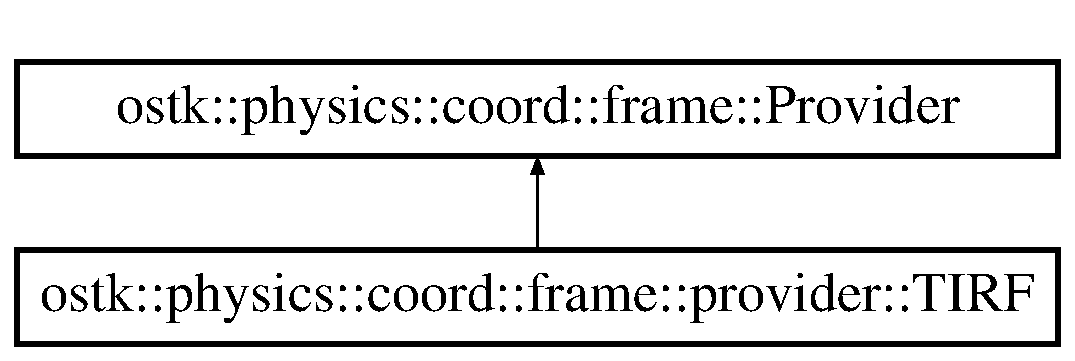
\includegraphics[height=2.000000cm]{classostk_1_1physics_1_1coord_1_1frame_1_1provider_1_1_t_i_r_f}
\end{center}
\end{figure}
\subsection*{Public Member Functions}
\begin{DoxyCompactItemize}
\item 
\hyperlink{classostk_1_1physics_1_1coord_1_1frame_1_1provider_1_1_t_i_r_f_ae2db654a92bdf9d29692edb5f62501b8}{T\+I\+RF} ()
\item 
virtual \hyperlink{classostk_1_1physics_1_1coord_1_1frame_1_1provider_1_1_t_i_r_f_a9b0da0362415d6dc45c9112d62cac7e5}{$\sim$\+T\+I\+RF} () override
\item 
virtual \hyperlink{classostk_1_1physics_1_1coord_1_1frame_1_1provider_1_1_t_i_r_f}{T\+I\+RF} $\ast$ \hyperlink{classostk_1_1physics_1_1coord_1_1frame_1_1provider_1_1_t_i_r_f_ae29e3db5bd1bccbc69a507f8716b73e5}{clone} () const override
\item 
virtual bool \hyperlink{classostk_1_1physics_1_1coord_1_1frame_1_1provider_1_1_t_i_r_f_ac7f3d815a45e270adab07bf6f51dc25f}{is\+Defined} () const override
\item 
virtual \hyperlink{classostk_1_1physics_1_1coord_1_1_transform}{Transform} \hyperlink{classostk_1_1physics_1_1coord_1_1frame_1_1provider_1_1_t_i_r_f_a23d651ab9857ad748e6bf3815205cd72}{get\+Transform\+At} (const \hyperlink{classostk_1_1physics_1_1time_1_1_instant}{Instant} \&an\+Instant) const override
\end{DoxyCompactItemize}


\subsection{Detailed Description}
Terrestrial Intermediate Reference \hyperlink{classostk_1_1physics_1_1coord_1_1_frame}{Frame} (\hyperlink{classostk_1_1physics_1_1coord_1_1frame_1_1provider_1_1_t_i_r_f}{T\+I\+RF}) provider. 

Earth rotation angle

https\+://www.iers.\+org/\+Shared\+Docs/\+Publikationen/\+E\+N/\+I\+E\+R\+S/\+Publications/tn/\+Techn\+Note36/tn36\+\_\+174.pdf?\+\_\+\+\_\+blob=publication\+File\&v=1 

\subsection{Constructor \& Destructor Documentation}
\mbox{\Hypertarget{classostk_1_1physics_1_1coord_1_1frame_1_1provider_1_1_t_i_r_f_ae2db654a92bdf9d29692edb5f62501b8}\label{classostk_1_1physics_1_1coord_1_1frame_1_1provider_1_1_t_i_r_f_ae2db654a92bdf9d29692edb5f62501b8}} 
\index{ostk\+::physics\+::coord\+::frame\+::provider\+::\+T\+I\+RF@{ostk\+::physics\+::coord\+::frame\+::provider\+::\+T\+I\+RF}!T\+I\+RF@{T\+I\+RF}}
\index{T\+I\+RF@{T\+I\+RF}!ostk\+::physics\+::coord\+::frame\+::provider\+::\+T\+I\+RF@{ostk\+::physics\+::coord\+::frame\+::provider\+::\+T\+I\+RF}}
\subsubsection{\texorpdfstring{T\+I\+R\+F()}{TIRF()}}
{\footnotesize\ttfamily ostk\+::physics\+::coord\+::frame\+::provider\+::\+T\+I\+R\+F\+::\+T\+I\+RF (\begin{DoxyParamCaption}{ }\end{DoxyParamCaption})}

\mbox{\Hypertarget{classostk_1_1physics_1_1coord_1_1frame_1_1provider_1_1_t_i_r_f_a9b0da0362415d6dc45c9112d62cac7e5}\label{classostk_1_1physics_1_1coord_1_1frame_1_1provider_1_1_t_i_r_f_a9b0da0362415d6dc45c9112d62cac7e5}} 
\index{ostk\+::physics\+::coord\+::frame\+::provider\+::\+T\+I\+RF@{ostk\+::physics\+::coord\+::frame\+::provider\+::\+T\+I\+RF}!````~T\+I\+RF@{$\sim$\+T\+I\+RF}}
\index{````~T\+I\+RF@{$\sim$\+T\+I\+RF}!ostk\+::physics\+::coord\+::frame\+::provider\+::\+T\+I\+RF@{ostk\+::physics\+::coord\+::frame\+::provider\+::\+T\+I\+RF}}
\subsubsection{\texorpdfstring{$\sim$\+T\+I\+R\+F()}{~TIRF()}}
{\footnotesize\ttfamily ostk\+::physics\+::coord\+::frame\+::provider\+::\+T\+I\+R\+F\+::$\sim$\+T\+I\+RF (\begin{DoxyParamCaption}{ }\end{DoxyParamCaption})\hspace{0.3cm}{\ttfamily [override]}, {\ttfamily [virtual]}}



\subsection{Member Function Documentation}
\mbox{\Hypertarget{classostk_1_1physics_1_1coord_1_1frame_1_1provider_1_1_t_i_r_f_ae29e3db5bd1bccbc69a507f8716b73e5}\label{classostk_1_1physics_1_1coord_1_1frame_1_1provider_1_1_t_i_r_f_ae29e3db5bd1bccbc69a507f8716b73e5}} 
\index{ostk\+::physics\+::coord\+::frame\+::provider\+::\+T\+I\+RF@{ostk\+::physics\+::coord\+::frame\+::provider\+::\+T\+I\+RF}!clone@{clone}}
\index{clone@{clone}!ostk\+::physics\+::coord\+::frame\+::provider\+::\+T\+I\+RF@{ostk\+::physics\+::coord\+::frame\+::provider\+::\+T\+I\+RF}}
\subsubsection{\texorpdfstring{clone()}{clone()}}
{\footnotesize\ttfamily \hyperlink{classostk_1_1physics_1_1coord_1_1frame_1_1provider_1_1_t_i_r_f}{T\+I\+RF} $\ast$ ostk\+::physics\+::coord\+::frame\+::provider\+::\+T\+I\+R\+F\+::clone (\begin{DoxyParamCaption}{ }\end{DoxyParamCaption}) const\hspace{0.3cm}{\ttfamily [override]}, {\ttfamily [virtual]}}



Implements \hyperlink{classostk_1_1physics_1_1coord_1_1frame_1_1_provider_ae41bc3862d088e9c8d90a79253294ce9}{ostk\+::physics\+::coord\+::frame\+::\+Provider}.

\mbox{\Hypertarget{classostk_1_1physics_1_1coord_1_1frame_1_1provider_1_1_t_i_r_f_a23d651ab9857ad748e6bf3815205cd72}\label{classostk_1_1physics_1_1coord_1_1frame_1_1provider_1_1_t_i_r_f_a23d651ab9857ad748e6bf3815205cd72}} 
\index{ostk\+::physics\+::coord\+::frame\+::provider\+::\+T\+I\+RF@{ostk\+::physics\+::coord\+::frame\+::provider\+::\+T\+I\+RF}!get\+Transform\+At@{get\+Transform\+At}}
\index{get\+Transform\+At@{get\+Transform\+At}!ostk\+::physics\+::coord\+::frame\+::provider\+::\+T\+I\+RF@{ostk\+::physics\+::coord\+::frame\+::provider\+::\+T\+I\+RF}}
\subsubsection{\texorpdfstring{get\+Transform\+At()}{getTransformAt()}}
{\footnotesize\ttfamily \hyperlink{classostk_1_1physics_1_1coord_1_1_transform}{Transform} ostk\+::physics\+::coord\+::frame\+::provider\+::\+T\+I\+R\+F\+::get\+Transform\+At (\begin{DoxyParamCaption}\item[{const \hyperlink{classostk_1_1physics_1_1time_1_1_instant}{Instant} \&}]{an\+Instant }\end{DoxyParamCaption}) const\hspace{0.3cm}{\ttfamily [override]}, {\ttfamily [virtual]}}



Implements \hyperlink{classostk_1_1physics_1_1coord_1_1frame_1_1_provider_a38b86a589f46f8b8a9c97ab2776f37d1}{ostk\+::physics\+::coord\+::frame\+::\+Provider}.

\mbox{\Hypertarget{classostk_1_1physics_1_1coord_1_1frame_1_1provider_1_1_t_i_r_f_ac7f3d815a45e270adab07bf6f51dc25f}\label{classostk_1_1physics_1_1coord_1_1frame_1_1provider_1_1_t_i_r_f_ac7f3d815a45e270adab07bf6f51dc25f}} 
\index{ostk\+::physics\+::coord\+::frame\+::provider\+::\+T\+I\+RF@{ostk\+::physics\+::coord\+::frame\+::provider\+::\+T\+I\+RF}!is\+Defined@{is\+Defined}}
\index{is\+Defined@{is\+Defined}!ostk\+::physics\+::coord\+::frame\+::provider\+::\+T\+I\+RF@{ostk\+::physics\+::coord\+::frame\+::provider\+::\+T\+I\+RF}}
\subsubsection{\texorpdfstring{is\+Defined()}{isDefined()}}
{\footnotesize\ttfamily bool ostk\+::physics\+::coord\+::frame\+::provider\+::\+T\+I\+R\+F\+::is\+Defined (\begin{DoxyParamCaption}{ }\end{DoxyParamCaption}) const\hspace{0.3cm}{\ttfamily [override]}, {\ttfamily [virtual]}}



Implements \hyperlink{classostk_1_1physics_1_1coord_1_1frame_1_1_provider_a27acab0012649796b97956fed1a91493}{ostk\+::physics\+::coord\+::frame\+::\+Provider}.



The documentation for this class was generated from the following files\+:\begin{DoxyCompactItemize}
\item 
include/\+Open\+Space\+Toolkit/\+Physics/\+Coordinate/\+Frame/\+Providers/\hyperlink{_t_i_r_f_8hpp}{T\+I\+R\+F.\+hpp}\item 
src/\+Open\+Space\+Toolkit/\+Physics/\+Coordinate/\+Frame/\+Providers/\hyperlink{_t_i_r_f_8cpp}{T\+I\+R\+F.\+cpp}\end{DoxyCompactItemize}

\hypertarget{classostk_1_1physics_1_1coord_1_1_transform}{}\section{ostk\+:\+:physics\+:\+:coord\+:\+:Transform Class Reference}
\label{classostk_1_1physics_1_1coord_1_1_transform}\index{ostk\+::physics\+::coord\+::\+Transform@{ostk\+::physics\+::coord\+::\+Transform}}


\hyperlink{classostk_1_1physics_1_1coord_1_1_transform}{Transform}.  




{\ttfamily \#include $<$Transform.\+hpp$>$}

\subsection*{Public Types}
\begin{DoxyCompactItemize}
\item 
enum \hyperlink{classostk_1_1physics_1_1coord_1_1_transform_a4325aff71186125b3ca8604247f55215}{Type} \{ \hyperlink{classostk_1_1physics_1_1coord_1_1_transform_a4325aff71186125b3ca8604247f55215aec0fc0100c4fc1ce4eea230c3dc10360}{Type\+::\+Undefined}, 
\hyperlink{classostk_1_1physics_1_1coord_1_1_transform_a4325aff71186125b3ca8604247f55215a4d3d769b812b6faa6b76e1a8abaece2d}{Type\+::\+Active}, 
\hyperlink{classostk_1_1physics_1_1coord_1_1_transform_a4325aff71186125b3ca8604247f55215af80bc338b6146b566004a046f8137c85}{Type\+::\+Passive}
 \}
\end{DoxyCompactItemize}
\subsection*{Public Member Functions}
\begin{DoxyCompactItemize}
\item 
\hyperlink{classostk_1_1physics_1_1coord_1_1_transform_a2117020ea022e73d64f7e4ac0c88ac46}{Transform} (const \hyperlink{classostk_1_1physics_1_1time_1_1_instant}{Instant} \&an\+Instant, const Vector3d \&a\+Translation, const Vector3d \&a\+Velocity, const Quaternion \&an\+Orientation, const Vector3d \&an\+Angular\+Velocity, const \hyperlink{classostk_1_1physics_1_1coord_1_1_transform_a4325aff71186125b3ca8604247f55215}{Transform\+::\+Type} \&a\+Type)
\item 
bool \hyperlink{classostk_1_1physics_1_1coord_1_1_transform_a0b1b8aa57021abeef185f69c4f0981ce}{operator==} (const \hyperlink{classostk_1_1physics_1_1coord_1_1_transform}{Transform} \&a\+Transform) const
\item 
bool \hyperlink{classostk_1_1physics_1_1coord_1_1_transform_a2dc5d65fdd5c364df815e5fa8b1f4b74}{operator!=} (const \hyperlink{classostk_1_1physics_1_1coord_1_1_transform}{Transform} \&a\+Transform) const
\item 
\hyperlink{classostk_1_1physics_1_1coord_1_1_transform}{Transform} \hyperlink{classostk_1_1physics_1_1coord_1_1_transform_ad596e25498b79fd0a5ae9a338c9a44e8}{operator$\ast$} (const \hyperlink{classostk_1_1physics_1_1coord_1_1_transform}{Transform} \&a\+Transform) const
\item 
\hyperlink{classostk_1_1physics_1_1coord_1_1_transform}{Transform} \& \hyperlink{classostk_1_1physics_1_1coord_1_1_transform_a63884c293c7f92e1a2fc0a33889dedc9}{operator$\ast$=} (const \hyperlink{classostk_1_1physics_1_1coord_1_1_transform}{Transform} \&a\+Transform)
\item 
bool \hyperlink{classostk_1_1physics_1_1coord_1_1_transform_a7bfe06d33b9aa8b62cc976b871bcc6ae}{is\+Defined} () const
\item 
bool \hyperlink{classostk_1_1physics_1_1coord_1_1_transform_a1519ff40a90b8ebc488cf926b7f9535b}{is\+Identity} () const
\item 
const \hyperlink{classostk_1_1physics_1_1time_1_1_instant}{Instant} \& \hyperlink{classostk_1_1physics_1_1coord_1_1_transform_a3b7d5279c94c3ff0cd324fc929eae533}{access\+Instant} () const
\item 
const Vector3d \& \hyperlink{classostk_1_1physics_1_1coord_1_1_transform_a5b5deef8d1a152934ce22334da35dffe}{access\+Translation} () const
\item 
const Vector3d \& \hyperlink{classostk_1_1physics_1_1coord_1_1_transform_a662ec4284f667bd704e9e003ea9924fd}{access\+Velocity} () const
\item 
const Quaternion \& \hyperlink{classostk_1_1physics_1_1coord_1_1_transform_aa246be611bf1928c9f67ffd6d2fe6e10}{access\+Orientation} () const
\item 
const Vector3d \& \hyperlink{classostk_1_1physics_1_1coord_1_1_transform_ae344e90f3419630a16d413224675a003}{access\+Angular\+Velocity} () const
\item 
\hyperlink{classostk_1_1physics_1_1time_1_1_instant}{Instant} \hyperlink{classostk_1_1physics_1_1coord_1_1_transform_a65a2cf0c24e5e2320b828d9bfb461d17}{get\+Instant} () const
\item 
Vector3d \hyperlink{classostk_1_1physics_1_1coord_1_1_transform_a1f54141f1d9c292e1767094e466320d0}{get\+Translation} () const
\item 
Vector3d \hyperlink{classostk_1_1physics_1_1coord_1_1_transform_a4a0a98719b6cc22ebb4dcb31cea7f0c9}{get\+Velocity} () const
\item 
Quaternion \hyperlink{classostk_1_1physics_1_1coord_1_1_transform_a21304f024b42a3d566166201df3ee5f9}{get\+Orientation} () const
\item 
Vector3d \hyperlink{classostk_1_1physics_1_1coord_1_1_transform_a54809903e2bd21032c461326427d56cc}{get\+Angular\+Velocity} () const
\item 
\hyperlink{classostk_1_1physics_1_1coord_1_1_transform}{Transform} \hyperlink{classostk_1_1physics_1_1coord_1_1_transform_a5ef781c60716faaf49befca0380285fe}{get\+Inverse} () const
\item 
Vector3d \hyperlink{classostk_1_1physics_1_1coord_1_1_transform_a1cdeac1d1e35d966c6c309d3507a6ccb}{apply\+To\+Position} (const Vector3d \&a\+Position) const
\item 
Vector3d \hyperlink{classostk_1_1physics_1_1coord_1_1_transform_a7d57f9e66f59711534ed8ba3e0719995}{apply\+To\+Velocity} (const Vector3d \&a\+Position, const Vector3d \&a\+Velocity) const
\item 
Vector3d \hyperlink{classostk_1_1physics_1_1coord_1_1_transform_a13f0ac6674ecb6748219f4ffc6a23e6e}{apply\+To\+Vector} (const Vector3d \&a\+Vector) const
\end{DoxyCompactItemize}
\subsection*{Static Public Member Functions}
\begin{DoxyCompactItemize}
\item 
static \hyperlink{classostk_1_1physics_1_1coord_1_1_transform}{Transform} \hyperlink{classostk_1_1physics_1_1coord_1_1_transform_a1271dd5a8f524e69b529538ca1871da7}{Undefined} ()
\item 
static \hyperlink{classostk_1_1physics_1_1coord_1_1_transform}{Transform} \hyperlink{classostk_1_1physics_1_1coord_1_1_transform_ab28461486f64cabd004ba99fc4c4b105}{Identity} (const \hyperlink{classostk_1_1physics_1_1time_1_1_instant}{Instant} \&an\+Instant)
\item 
static \hyperlink{classostk_1_1physics_1_1coord_1_1_transform}{Transform} \hyperlink{classostk_1_1physics_1_1coord_1_1_transform_a0e28392ffaf90f9a3a75bef3f0d612d3}{Active} (const \hyperlink{classostk_1_1physics_1_1time_1_1_instant}{Instant} \&an\+Instant, const Vector3d \&a\+Translation, const Vector3d \&a\+Velocity, const Quaternion \&an\+Orientation, const Vector3d \&an\+Angular\+Velocity)
\item 
static \hyperlink{classostk_1_1physics_1_1coord_1_1_transform}{Transform} \hyperlink{classostk_1_1physics_1_1coord_1_1_transform_af8df2e5e9b476720bee05301079eb908}{Passive} (const \hyperlink{classostk_1_1physics_1_1time_1_1_instant}{Instant} \&an\+Instant, const Vector3d \&a\+Translation, const Vector3d \&a\+Velocity, const Quaternion \&an\+Orientation, const Vector3d \&an\+Angular\+Velocity)
\end{DoxyCompactItemize}
\subsection*{Friends}
\begin{DoxyCompactItemize}
\item 
std\+::ostream \& \hyperlink{classostk_1_1physics_1_1coord_1_1_transform_ae46ab7a297c23b757fd6f41bf30c4054}{operator$<$$<$} (std\+::ostream \&an\+Output\+Stream, const \hyperlink{classostk_1_1physics_1_1coord_1_1_transform}{Transform} \&a\+Transform)
\end{DoxyCompactItemize}


\subsection{Detailed Description}
\hyperlink{classostk_1_1physics_1_1coord_1_1_transform}{Transform}. 

Passive transformation

https\+://en.wikipedia.\+org/wiki/\+Active\+\_\+and\+\_\+passive\+\_\+transformation https\+://core.ac.\+uk/download/pdf/77055186.pdf 

\subsection{Member Enumeration Documentation}
\mbox{\Hypertarget{classostk_1_1physics_1_1coord_1_1_transform_a4325aff71186125b3ca8604247f55215}\label{classostk_1_1physics_1_1coord_1_1_transform_a4325aff71186125b3ca8604247f55215}} 
\index{ostk\+::physics\+::coord\+::\+Transform@{ostk\+::physics\+::coord\+::\+Transform}!Type@{Type}}
\index{Type@{Type}!ostk\+::physics\+::coord\+::\+Transform@{ostk\+::physics\+::coord\+::\+Transform}}
\subsubsection{\texorpdfstring{Type}{Type}}
{\footnotesize\ttfamily enum \hyperlink{classostk_1_1physics_1_1coord_1_1_transform_a4325aff71186125b3ca8604247f55215}{ostk\+::physics\+::coord\+::\+Transform\+::\+Type}\hspace{0.3cm}{\ttfamily [strong]}}

\begin{DoxyEnumFields}{Enumerator}
\raisebox{\heightof{T}}[0pt][0pt]{\index{Undefined@{Undefined}!ostk\+::physics\+::coord\+::\+Transform@{ostk\+::physics\+::coord\+::\+Transform}}\index{ostk\+::physics\+::coord\+::\+Transform@{ostk\+::physics\+::coord\+::\+Transform}!Undefined@{Undefined}}}\mbox{\Hypertarget{classostk_1_1physics_1_1coord_1_1_transform_a4325aff71186125b3ca8604247f55215aec0fc0100c4fc1ce4eea230c3dc10360}\label{classostk_1_1physics_1_1coord_1_1_transform_a4325aff71186125b3ca8604247f55215aec0fc0100c4fc1ce4eea230c3dc10360}} 
Undefined&\\
\hline

\raisebox{\heightof{T}}[0pt][0pt]{\index{Active@{Active}!ostk\+::physics\+::coord\+::\+Transform@{ostk\+::physics\+::coord\+::\+Transform}}\index{ostk\+::physics\+::coord\+::\+Transform@{ostk\+::physics\+::coord\+::\+Transform}!Active@{Active}}}\mbox{\Hypertarget{classostk_1_1physics_1_1coord_1_1_transform_a4325aff71186125b3ca8604247f55215a4d3d769b812b6faa6b76e1a8abaece2d}\label{classostk_1_1physics_1_1coord_1_1_transform_a4325aff71186125b3ca8604247f55215a4d3d769b812b6faa6b76e1a8abaece2d}} 
Active&\\
\hline

\raisebox{\heightof{T}}[0pt][0pt]{\index{Passive@{Passive}!ostk\+::physics\+::coord\+::\+Transform@{ostk\+::physics\+::coord\+::\+Transform}}\index{ostk\+::physics\+::coord\+::\+Transform@{ostk\+::physics\+::coord\+::\+Transform}!Passive@{Passive}}}\mbox{\Hypertarget{classostk_1_1physics_1_1coord_1_1_transform_a4325aff71186125b3ca8604247f55215af80bc338b6146b566004a046f8137c85}\label{classostk_1_1physics_1_1coord_1_1_transform_a4325aff71186125b3ca8604247f55215af80bc338b6146b566004a046f8137c85}} 
Passive&\\
\hline

\end{DoxyEnumFields}


\subsection{Constructor \& Destructor Documentation}
\mbox{\Hypertarget{classostk_1_1physics_1_1coord_1_1_transform_a2117020ea022e73d64f7e4ac0c88ac46}\label{classostk_1_1physics_1_1coord_1_1_transform_a2117020ea022e73d64f7e4ac0c88ac46}} 
\index{ostk\+::physics\+::coord\+::\+Transform@{ostk\+::physics\+::coord\+::\+Transform}!Transform@{Transform}}
\index{Transform@{Transform}!ostk\+::physics\+::coord\+::\+Transform@{ostk\+::physics\+::coord\+::\+Transform}}
\subsubsection{\texorpdfstring{Transform()}{Transform()}}
{\footnotesize\ttfamily ostk\+::physics\+::coord\+::\+Transform\+::\+Transform (\begin{DoxyParamCaption}\item[{const \hyperlink{classostk_1_1physics_1_1time_1_1_instant}{Instant} \&}]{an\+Instant,  }\item[{const Vector3d \&}]{a\+Translation,  }\item[{const Vector3d \&}]{a\+Velocity,  }\item[{const Quaternion \&}]{an\+Orientation,  }\item[{const Vector3d \&}]{an\+Angular\+Velocity,  }\item[{const \hyperlink{classostk_1_1physics_1_1coord_1_1_transform_a4325aff71186125b3ca8604247f55215}{Transform\+::\+Type} \&}]{a\+Type }\end{DoxyParamCaption})}



\subsection{Member Function Documentation}
\mbox{\Hypertarget{classostk_1_1physics_1_1coord_1_1_transform_ae344e90f3419630a16d413224675a003}\label{classostk_1_1physics_1_1coord_1_1_transform_ae344e90f3419630a16d413224675a003}} 
\index{ostk\+::physics\+::coord\+::\+Transform@{ostk\+::physics\+::coord\+::\+Transform}!access\+Angular\+Velocity@{access\+Angular\+Velocity}}
\index{access\+Angular\+Velocity@{access\+Angular\+Velocity}!ostk\+::physics\+::coord\+::\+Transform@{ostk\+::physics\+::coord\+::\+Transform}}
\subsubsection{\texorpdfstring{access\+Angular\+Velocity()}{accessAngularVelocity()}}
{\footnotesize\ttfamily const Vector3d \& ostk\+::physics\+::coord\+::\+Transform\+::access\+Angular\+Velocity (\begin{DoxyParamCaption}{ }\end{DoxyParamCaption}) const}

\mbox{\Hypertarget{classostk_1_1physics_1_1coord_1_1_transform_a3b7d5279c94c3ff0cd324fc929eae533}\label{classostk_1_1physics_1_1coord_1_1_transform_a3b7d5279c94c3ff0cd324fc929eae533}} 
\index{ostk\+::physics\+::coord\+::\+Transform@{ostk\+::physics\+::coord\+::\+Transform}!access\+Instant@{access\+Instant}}
\index{access\+Instant@{access\+Instant}!ostk\+::physics\+::coord\+::\+Transform@{ostk\+::physics\+::coord\+::\+Transform}}
\subsubsection{\texorpdfstring{access\+Instant()}{accessInstant()}}
{\footnotesize\ttfamily const \hyperlink{classostk_1_1physics_1_1time_1_1_instant}{Instant} \& ostk\+::physics\+::coord\+::\+Transform\+::access\+Instant (\begin{DoxyParamCaption}{ }\end{DoxyParamCaption}) const}

\mbox{\Hypertarget{classostk_1_1physics_1_1coord_1_1_transform_aa246be611bf1928c9f67ffd6d2fe6e10}\label{classostk_1_1physics_1_1coord_1_1_transform_aa246be611bf1928c9f67ffd6d2fe6e10}} 
\index{ostk\+::physics\+::coord\+::\+Transform@{ostk\+::physics\+::coord\+::\+Transform}!access\+Orientation@{access\+Orientation}}
\index{access\+Orientation@{access\+Orientation}!ostk\+::physics\+::coord\+::\+Transform@{ostk\+::physics\+::coord\+::\+Transform}}
\subsubsection{\texorpdfstring{access\+Orientation()}{accessOrientation()}}
{\footnotesize\ttfamily const Quaternion \& ostk\+::physics\+::coord\+::\+Transform\+::access\+Orientation (\begin{DoxyParamCaption}{ }\end{DoxyParamCaption}) const}

\mbox{\Hypertarget{classostk_1_1physics_1_1coord_1_1_transform_a5b5deef8d1a152934ce22334da35dffe}\label{classostk_1_1physics_1_1coord_1_1_transform_a5b5deef8d1a152934ce22334da35dffe}} 
\index{ostk\+::physics\+::coord\+::\+Transform@{ostk\+::physics\+::coord\+::\+Transform}!access\+Translation@{access\+Translation}}
\index{access\+Translation@{access\+Translation}!ostk\+::physics\+::coord\+::\+Transform@{ostk\+::physics\+::coord\+::\+Transform}}
\subsubsection{\texorpdfstring{access\+Translation()}{accessTranslation()}}
{\footnotesize\ttfamily const Vector3d \& ostk\+::physics\+::coord\+::\+Transform\+::access\+Translation (\begin{DoxyParamCaption}{ }\end{DoxyParamCaption}) const}

\mbox{\Hypertarget{classostk_1_1physics_1_1coord_1_1_transform_a662ec4284f667bd704e9e003ea9924fd}\label{classostk_1_1physics_1_1coord_1_1_transform_a662ec4284f667bd704e9e003ea9924fd}} 
\index{ostk\+::physics\+::coord\+::\+Transform@{ostk\+::physics\+::coord\+::\+Transform}!access\+Velocity@{access\+Velocity}}
\index{access\+Velocity@{access\+Velocity}!ostk\+::physics\+::coord\+::\+Transform@{ostk\+::physics\+::coord\+::\+Transform}}
\subsubsection{\texorpdfstring{access\+Velocity()}{accessVelocity()}}
{\footnotesize\ttfamily const Vector3d \& ostk\+::physics\+::coord\+::\+Transform\+::access\+Velocity (\begin{DoxyParamCaption}{ }\end{DoxyParamCaption}) const}

\mbox{\Hypertarget{classostk_1_1physics_1_1coord_1_1_transform_a0e28392ffaf90f9a3a75bef3f0d612d3}\label{classostk_1_1physics_1_1coord_1_1_transform_a0e28392ffaf90f9a3a75bef3f0d612d3}} 
\index{ostk\+::physics\+::coord\+::\+Transform@{ostk\+::physics\+::coord\+::\+Transform}!Active@{Active}}
\index{Active@{Active}!ostk\+::physics\+::coord\+::\+Transform@{ostk\+::physics\+::coord\+::\+Transform}}
\subsubsection{\texorpdfstring{Active()}{Active()}}
{\footnotesize\ttfamily \hyperlink{classostk_1_1physics_1_1coord_1_1_transform}{Transform} ostk\+::physics\+::coord\+::\+Transform\+::\+Active (\begin{DoxyParamCaption}\item[{const \hyperlink{classostk_1_1physics_1_1time_1_1_instant}{Instant} \&}]{an\+Instant,  }\item[{const Vector3d \&}]{a\+Translation,  }\item[{const Vector3d \&}]{a\+Velocity,  }\item[{const Quaternion \&}]{an\+Orientation,  }\item[{const Vector3d \&}]{an\+Angular\+Velocity }\end{DoxyParamCaption})\hspace{0.3cm}{\ttfamily [static]}}

\mbox{\Hypertarget{classostk_1_1physics_1_1coord_1_1_transform_a1cdeac1d1e35d966c6c309d3507a6ccb}\label{classostk_1_1physics_1_1coord_1_1_transform_a1cdeac1d1e35d966c6c309d3507a6ccb}} 
\index{ostk\+::physics\+::coord\+::\+Transform@{ostk\+::physics\+::coord\+::\+Transform}!apply\+To\+Position@{apply\+To\+Position}}
\index{apply\+To\+Position@{apply\+To\+Position}!ostk\+::physics\+::coord\+::\+Transform@{ostk\+::physics\+::coord\+::\+Transform}}
\subsubsection{\texorpdfstring{apply\+To\+Position()}{applyToPosition()}}
{\footnotesize\ttfamily Vector3d ostk\+::physics\+::coord\+::\+Transform\+::apply\+To\+Position (\begin{DoxyParamCaption}\item[{const Vector3d \&}]{a\+Position }\end{DoxyParamCaption}) const}

\mbox{\Hypertarget{classostk_1_1physics_1_1coord_1_1_transform_a13f0ac6674ecb6748219f4ffc6a23e6e}\label{classostk_1_1physics_1_1coord_1_1_transform_a13f0ac6674ecb6748219f4ffc6a23e6e}} 
\index{ostk\+::physics\+::coord\+::\+Transform@{ostk\+::physics\+::coord\+::\+Transform}!apply\+To\+Vector@{apply\+To\+Vector}}
\index{apply\+To\+Vector@{apply\+To\+Vector}!ostk\+::physics\+::coord\+::\+Transform@{ostk\+::physics\+::coord\+::\+Transform}}
\subsubsection{\texorpdfstring{apply\+To\+Vector()}{applyToVector()}}
{\footnotesize\ttfamily Vector3d ostk\+::physics\+::coord\+::\+Transform\+::apply\+To\+Vector (\begin{DoxyParamCaption}\item[{const Vector3d \&}]{a\+Vector }\end{DoxyParamCaption}) const}

\mbox{\Hypertarget{classostk_1_1physics_1_1coord_1_1_transform_a7d57f9e66f59711534ed8ba3e0719995}\label{classostk_1_1physics_1_1coord_1_1_transform_a7d57f9e66f59711534ed8ba3e0719995}} 
\index{ostk\+::physics\+::coord\+::\+Transform@{ostk\+::physics\+::coord\+::\+Transform}!apply\+To\+Velocity@{apply\+To\+Velocity}}
\index{apply\+To\+Velocity@{apply\+To\+Velocity}!ostk\+::physics\+::coord\+::\+Transform@{ostk\+::physics\+::coord\+::\+Transform}}
\subsubsection{\texorpdfstring{apply\+To\+Velocity()}{applyToVelocity()}}
{\footnotesize\ttfamily Vector3d ostk\+::physics\+::coord\+::\+Transform\+::apply\+To\+Velocity (\begin{DoxyParamCaption}\item[{const Vector3d \&}]{a\+Position,  }\item[{const Vector3d \&}]{a\+Velocity }\end{DoxyParamCaption}) const}

\mbox{\Hypertarget{classostk_1_1physics_1_1coord_1_1_transform_a54809903e2bd21032c461326427d56cc}\label{classostk_1_1physics_1_1coord_1_1_transform_a54809903e2bd21032c461326427d56cc}} 
\index{ostk\+::physics\+::coord\+::\+Transform@{ostk\+::physics\+::coord\+::\+Transform}!get\+Angular\+Velocity@{get\+Angular\+Velocity}}
\index{get\+Angular\+Velocity@{get\+Angular\+Velocity}!ostk\+::physics\+::coord\+::\+Transform@{ostk\+::physics\+::coord\+::\+Transform}}
\subsubsection{\texorpdfstring{get\+Angular\+Velocity()}{getAngularVelocity()}}
{\footnotesize\ttfamily Vector3d ostk\+::physics\+::coord\+::\+Transform\+::get\+Angular\+Velocity (\begin{DoxyParamCaption}{ }\end{DoxyParamCaption}) const}

\mbox{\Hypertarget{classostk_1_1physics_1_1coord_1_1_transform_a65a2cf0c24e5e2320b828d9bfb461d17}\label{classostk_1_1physics_1_1coord_1_1_transform_a65a2cf0c24e5e2320b828d9bfb461d17}} 
\index{ostk\+::physics\+::coord\+::\+Transform@{ostk\+::physics\+::coord\+::\+Transform}!get\+Instant@{get\+Instant}}
\index{get\+Instant@{get\+Instant}!ostk\+::physics\+::coord\+::\+Transform@{ostk\+::physics\+::coord\+::\+Transform}}
\subsubsection{\texorpdfstring{get\+Instant()}{getInstant()}}
{\footnotesize\ttfamily \hyperlink{classostk_1_1physics_1_1time_1_1_instant}{Instant} ostk\+::physics\+::coord\+::\+Transform\+::get\+Instant (\begin{DoxyParamCaption}{ }\end{DoxyParamCaption}) const}

\mbox{\Hypertarget{classostk_1_1physics_1_1coord_1_1_transform_a5ef781c60716faaf49befca0380285fe}\label{classostk_1_1physics_1_1coord_1_1_transform_a5ef781c60716faaf49befca0380285fe}} 
\index{ostk\+::physics\+::coord\+::\+Transform@{ostk\+::physics\+::coord\+::\+Transform}!get\+Inverse@{get\+Inverse}}
\index{get\+Inverse@{get\+Inverse}!ostk\+::physics\+::coord\+::\+Transform@{ostk\+::physics\+::coord\+::\+Transform}}
\subsubsection{\texorpdfstring{get\+Inverse()}{getInverse()}}
{\footnotesize\ttfamily \hyperlink{classostk_1_1physics_1_1coord_1_1_transform}{Transform} ostk\+::physics\+::coord\+::\+Transform\+::get\+Inverse (\begin{DoxyParamCaption}{ }\end{DoxyParamCaption}) const}

\mbox{\Hypertarget{classostk_1_1physics_1_1coord_1_1_transform_a21304f024b42a3d566166201df3ee5f9}\label{classostk_1_1physics_1_1coord_1_1_transform_a21304f024b42a3d566166201df3ee5f9}} 
\index{ostk\+::physics\+::coord\+::\+Transform@{ostk\+::physics\+::coord\+::\+Transform}!get\+Orientation@{get\+Orientation}}
\index{get\+Orientation@{get\+Orientation}!ostk\+::physics\+::coord\+::\+Transform@{ostk\+::physics\+::coord\+::\+Transform}}
\subsubsection{\texorpdfstring{get\+Orientation()}{getOrientation()}}
{\footnotesize\ttfamily Quaternion ostk\+::physics\+::coord\+::\+Transform\+::get\+Orientation (\begin{DoxyParamCaption}{ }\end{DoxyParamCaption}) const}

\mbox{\Hypertarget{classostk_1_1physics_1_1coord_1_1_transform_a1f54141f1d9c292e1767094e466320d0}\label{classostk_1_1physics_1_1coord_1_1_transform_a1f54141f1d9c292e1767094e466320d0}} 
\index{ostk\+::physics\+::coord\+::\+Transform@{ostk\+::physics\+::coord\+::\+Transform}!get\+Translation@{get\+Translation}}
\index{get\+Translation@{get\+Translation}!ostk\+::physics\+::coord\+::\+Transform@{ostk\+::physics\+::coord\+::\+Transform}}
\subsubsection{\texorpdfstring{get\+Translation()}{getTranslation()}}
{\footnotesize\ttfamily Vector3d ostk\+::physics\+::coord\+::\+Transform\+::get\+Translation (\begin{DoxyParamCaption}{ }\end{DoxyParamCaption}) const}

\mbox{\Hypertarget{classostk_1_1physics_1_1coord_1_1_transform_a4a0a98719b6cc22ebb4dcb31cea7f0c9}\label{classostk_1_1physics_1_1coord_1_1_transform_a4a0a98719b6cc22ebb4dcb31cea7f0c9}} 
\index{ostk\+::physics\+::coord\+::\+Transform@{ostk\+::physics\+::coord\+::\+Transform}!get\+Velocity@{get\+Velocity}}
\index{get\+Velocity@{get\+Velocity}!ostk\+::physics\+::coord\+::\+Transform@{ostk\+::physics\+::coord\+::\+Transform}}
\subsubsection{\texorpdfstring{get\+Velocity()}{getVelocity()}}
{\footnotesize\ttfamily Vector3d ostk\+::physics\+::coord\+::\+Transform\+::get\+Velocity (\begin{DoxyParamCaption}{ }\end{DoxyParamCaption}) const}

\mbox{\Hypertarget{classostk_1_1physics_1_1coord_1_1_transform_ab28461486f64cabd004ba99fc4c4b105}\label{classostk_1_1physics_1_1coord_1_1_transform_ab28461486f64cabd004ba99fc4c4b105}} 
\index{ostk\+::physics\+::coord\+::\+Transform@{ostk\+::physics\+::coord\+::\+Transform}!Identity@{Identity}}
\index{Identity@{Identity}!ostk\+::physics\+::coord\+::\+Transform@{ostk\+::physics\+::coord\+::\+Transform}}
\subsubsection{\texorpdfstring{Identity()}{Identity()}}
{\footnotesize\ttfamily \hyperlink{classostk_1_1physics_1_1coord_1_1_transform}{Transform} ostk\+::physics\+::coord\+::\+Transform\+::\+Identity (\begin{DoxyParamCaption}\item[{const \hyperlink{classostk_1_1physics_1_1time_1_1_instant}{Instant} \&}]{an\+Instant }\end{DoxyParamCaption})\hspace{0.3cm}{\ttfamily [static]}}

\mbox{\Hypertarget{classostk_1_1physics_1_1coord_1_1_transform_a7bfe06d33b9aa8b62cc976b871bcc6ae}\label{classostk_1_1physics_1_1coord_1_1_transform_a7bfe06d33b9aa8b62cc976b871bcc6ae}} 
\index{ostk\+::physics\+::coord\+::\+Transform@{ostk\+::physics\+::coord\+::\+Transform}!is\+Defined@{is\+Defined}}
\index{is\+Defined@{is\+Defined}!ostk\+::physics\+::coord\+::\+Transform@{ostk\+::physics\+::coord\+::\+Transform}}
\subsubsection{\texorpdfstring{is\+Defined()}{isDefined()}}
{\footnotesize\ttfamily bool ostk\+::physics\+::coord\+::\+Transform\+::is\+Defined (\begin{DoxyParamCaption}{ }\end{DoxyParamCaption}) const}

\mbox{\Hypertarget{classostk_1_1physics_1_1coord_1_1_transform_a1519ff40a90b8ebc488cf926b7f9535b}\label{classostk_1_1physics_1_1coord_1_1_transform_a1519ff40a90b8ebc488cf926b7f9535b}} 
\index{ostk\+::physics\+::coord\+::\+Transform@{ostk\+::physics\+::coord\+::\+Transform}!is\+Identity@{is\+Identity}}
\index{is\+Identity@{is\+Identity}!ostk\+::physics\+::coord\+::\+Transform@{ostk\+::physics\+::coord\+::\+Transform}}
\subsubsection{\texorpdfstring{is\+Identity()}{isIdentity()}}
{\footnotesize\ttfamily bool ostk\+::physics\+::coord\+::\+Transform\+::is\+Identity (\begin{DoxyParamCaption}{ }\end{DoxyParamCaption}) const}

\mbox{\Hypertarget{classostk_1_1physics_1_1coord_1_1_transform_a2dc5d65fdd5c364df815e5fa8b1f4b74}\label{classostk_1_1physics_1_1coord_1_1_transform_a2dc5d65fdd5c364df815e5fa8b1f4b74}} 
\index{ostk\+::physics\+::coord\+::\+Transform@{ostk\+::physics\+::coord\+::\+Transform}!operator"!=@{operator"!=}}
\index{operator"!=@{operator"!=}!ostk\+::physics\+::coord\+::\+Transform@{ostk\+::physics\+::coord\+::\+Transform}}
\subsubsection{\texorpdfstring{operator"!=()}{operator!=()}}
{\footnotesize\ttfamily bool ostk\+::physics\+::coord\+::\+Transform\+::operator!= (\begin{DoxyParamCaption}\item[{const \hyperlink{classostk_1_1physics_1_1coord_1_1_transform}{Transform} \&}]{a\+Transform }\end{DoxyParamCaption}) const}

\mbox{\Hypertarget{classostk_1_1physics_1_1coord_1_1_transform_ad596e25498b79fd0a5ae9a338c9a44e8}\label{classostk_1_1physics_1_1coord_1_1_transform_ad596e25498b79fd0a5ae9a338c9a44e8}} 
\index{ostk\+::physics\+::coord\+::\+Transform@{ostk\+::physics\+::coord\+::\+Transform}!operator$\ast$@{operator$\ast$}}
\index{operator$\ast$@{operator$\ast$}!ostk\+::physics\+::coord\+::\+Transform@{ostk\+::physics\+::coord\+::\+Transform}}
\subsubsection{\texorpdfstring{operator$\ast$()}{operator*()}}
{\footnotesize\ttfamily \hyperlink{classostk_1_1physics_1_1coord_1_1_transform}{Transform} ostk\+::physics\+::coord\+::\+Transform\+::operator$\ast$ (\begin{DoxyParamCaption}\item[{const \hyperlink{classostk_1_1physics_1_1coord_1_1_transform}{Transform} \&}]{a\+Transform }\end{DoxyParamCaption}) const}

\mbox{\Hypertarget{classostk_1_1physics_1_1coord_1_1_transform_a63884c293c7f92e1a2fc0a33889dedc9}\label{classostk_1_1physics_1_1coord_1_1_transform_a63884c293c7f92e1a2fc0a33889dedc9}} 
\index{ostk\+::physics\+::coord\+::\+Transform@{ostk\+::physics\+::coord\+::\+Transform}!operator$\ast$=@{operator$\ast$=}}
\index{operator$\ast$=@{operator$\ast$=}!ostk\+::physics\+::coord\+::\+Transform@{ostk\+::physics\+::coord\+::\+Transform}}
\subsubsection{\texorpdfstring{operator$\ast$=()}{operator*=()}}
{\footnotesize\ttfamily \hyperlink{classostk_1_1physics_1_1coord_1_1_transform}{Transform} \& ostk\+::physics\+::coord\+::\+Transform\+::operator$\ast$= (\begin{DoxyParamCaption}\item[{const \hyperlink{classostk_1_1physics_1_1coord_1_1_transform}{Transform} \&}]{a\+Transform }\end{DoxyParamCaption})}

\mbox{\Hypertarget{classostk_1_1physics_1_1coord_1_1_transform_a0b1b8aa57021abeef185f69c4f0981ce}\label{classostk_1_1physics_1_1coord_1_1_transform_a0b1b8aa57021abeef185f69c4f0981ce}} 
\index{ostk\+::physics\+::coord\+::\+Transform@{ostk\+::physics\+::coord\+::\+Transform}!operator==@{operator==}}
\index{operator==@{operator==}!ostk\+::physics\+::coord\+::\+Transform@{ostk\+::physics\+::coord\+::\+Transform}}
\subsubsection{\texorpdfstring{operator==()}{operator==()}}
{\footnotesize\ttfamily bool ostk\+::physics\+::coord\+::\+Transform\+::operator== (\begin{DoxyParamCaption}\item[{const \hyperlink{classostk_1_1physics_1_1coord_1_1_transform}{Transform} \&}]{a\+Transform }\end{DoxyParamCaption}) const}

\mbox{\Hypertarget{classostk_1_1physics_1_1coord_1_1_transform_af8df2e5e9b476720bee05301079eb908}\label{classostk_1_1physics_1_1coord_1_1_transform_af8df2e5e9b476720bee05301079eb908}} 
\index{ostk\+::physics\+::coord\+::\+Transform@{ostk\+::physics\+::coord\+::\+Transform}!Passive@{Passive}}
\index{Passive@{Passive}!ostk\+::physics\+::coord\+::\+Transform@{ostk\+::physics\+::coord\+::\+Transform}}
\subsubsection{\texorpdfstring{Passive()}{Passive()}}
{\footnotesize\ttfamily \hyperlink{classostk_1_1physics_1_1coord_1_1_transform}{Transform} ostk\+::physics\+::coord\+::\+Transform\+::\+Passive (\begin{DoxyParamCaption}\item[{const \hyperlink{classostk_1_1physics_1_1time_1_1_instant}{Instant} \&}]{an\+Instant,  }\item[{const Vector3d \&}]{a\+Translation,  }\item[{const Vector3d \&}]{a\+Velocity,  }\item[{const Quaternion \&}]{an\+Orientation,  }\item[{const Vector3d \&}]{an\+Angular\+Velocity }\end{DoxyParamCaption})\hspace{0.3cm}{\ttfamily [static]}}

\mbox{\Hypertarget{classostk_1_1physics_1_1coord_1_1_transform_a1271dd5a8f524e69b529538ca1871da7}\label{classostk_1_1physics_1_1coord_1_1_transform_a1271dd5a8f524e69b529538ca1871da7}} 
\index{ostk\+::physics\+::coord\+::\+Transform@{ostk\+::physics\+::coord\+::\+Transform}!Undefined@{Undefined}}
\index{Undefined@{Undefined}!ostk\+::physics\+::coord\+::\+Transform@{ostk\+::physics\+::coord\+::\+Transform}}
\subsubsection{\texorpdfstring{Undefined()}{Undefined()}}
{\footnotesize\ttfamily \hyperlink{classostk_1_1physics_1_1coord_1_1_transform}{Transform} ostk\+::physics\+::coord\+::\+Transform\+::\+Undefined (\begin{DoxyParamCaption}{ }\end{DoxyParamCaption})\hspace{0.3cm}{\ttfamily [static]}}



\subsection{Friends And Related Function Documentation}
\mbox{\Hypertarget{classostk_1_1physics_1_1coord_1_1_transform_ae46ab7a297c23b757fd6f41bf30c4054}\label{classostk_1_1physics_1_1coord_1_1_transform_ae46ab7a297c23b757fd6f41bf30c4054}} 
\index{ostk\+::physics\+::coord\+::\+Transform@{ostk\+::physics\+::coord\+::\+Transform}!operator$<$$<$@{operator$<$$<$}}
\index{operator$<$$<$@{operator$<$$<$}!ostk\+::physics\+::coord\+::\+Transform@{ostk\+::physics\+::coord\+::\+Transform}}
\subsubsection{\texorpdfstring{operator$<$$<$}{operator<<}}
{\footnotesize\ttfamily std\+::ostream\& operator$<$$<$ (\begin{DoxyParamCaption}\item[{std\+::ostream \&}]{an\+Output\+Stream,  }\item[{const \hyperlink{classostk_1_1physics_1_1coord_1_1_transform}{Transform} \&}]{a\+Transform }\end{DoxyParamCaption})\hspace{0.3cm}{\ttfamily [friend]}}



The documentation for this class was generated from the following files\+:\begin{DoxyCompactItemize}
\item 
include/\+Open\+Space\+Toolkit/\+Physics/\+Coordinate/\hyperlink{_transform_8hpp}{Transform.\+hpp}\item 
src/\+Open\+Space\+Toolkit/\+Physics/\+Coordinate/\hyperlink{_transform_8cpp}{Transform.\+cpp}\end{DoxyCompactItemize}

\hypertarget{classostk_1_1physics_1_1units_1_1_derived_1_1_unit}{}\section{ostk\+:\+:physics\+:\+:units\+:\+:Derived\+:\+:Unit Class Reference}
\label{classostk_1_1physics_1_1units_1_1_derived_1_1_unit}\index{ostk\+::physics\+::units\+::\+Derived\+::\+Unit@{ostk\+::physics\+::units\+::\+Derived\+::\+Unit}}


\hyperlink{classostk_1_1physics_1_1units_1_1_derived_1_1_unit}{Unit}.  




{\ttfamily \#include $<$Derived.\+hpp$>$}

\subsection*{Public Member Functions}
\begin{DoxyCompactItemize}
\item 
\hyperlink{classostk_1_1physics_1_1units_1_1_derived_1_1_unit_a2f40f9bd4c0d94f13c5a4cd4e6d7a91c}{Unit} (const \hyperlink{classostk_1_1physics_1_1units_1_1_length_a2664470a7eedf5d45c88861fe69badea}{Length\+::\+Unit} \&a\+Length\+Unit, const \hyperlink{classostk_1_1physics_1_1units_1_1_derived_1_1_order}{Order} \&a\+Length\+Order, const \hyperlink{classostk_1_1physics_1_1units_1_1_mass_aa8994892478fdbe6dc78d4bca08db0fa}{Mass\+::\+Unit} \&a\+Mass\+Unit, const \hyperlink{classostk_1_1physics_1_1units_1_1_derived_1_1_order}{Order} \&a\+Mass\+Order, const \hyperlink{classostk_1_1physics_1_1units_1_1_time_aa961f0dbca7ec297e19e15e0dfa3bb4a}{Time\+::\+Unit} \&a\+Time\+Unit, const \hyperlink{classostk_1_1physics_1_1units_1_1_derived_1_1_order}{Order} \&a\+Time\+Order, const \hyperlink{classostk_1_1physics_1_1units_1_1_electric_current_ac57c87a7533dc73b87185b0d9ae6985b}{Electric\+Current\+::\+Unit} \&an\+Electric\+Current\+Unit, const \hyperlink{classostk_1_1physics_1_1units_1_1_derived_1_1_order}{Order} \&an\+Electric\+Current\+Order, const \hyperlink{classostk_1_1physics_1_1units_1_1_angle_aea1f8018b1d378b9dee56959d8eb9def}{Angle\+::\+Unit} \&an\+Angle\+Unit, const \hyperlink{classostk_1_1physics_1_1units_1_1_derived_1_1_order}{Order} \&an\+Angle\+Order)
\item 
bool \hyperlink{classostk_1_1physics_1_1units_1_1_derived_1_1_unit_af585bf9564ac42ca3d82bb2a58fe4465}{operator==} (const \hyperlink{classostk_1_1physics_1_1units_1_1_derived_1_1_unit}{Unit} \&a\+Unit) const
\item 
bool \hyperlink{classostk_1_1physics_1_1units_1_1_derived_1_1_unit_a488e9bfa1834dbf6a7807fc9d3d00271}{operator!=} (const \hyperlink{classostk_1_1physics_1_1units_1_1_derived_1_1_unit}{Unit} \&a\+Unit) const
\item 
bool \hyperlink{classostk_1_1physics_1_1units_1_1_derived_1_1_unit_a24e22ed8550220e0d4235a35374be0a4}{is\+Defined} () const
\item 
bool \hyperlink{classostk_1_1physics_1_1units_1_1_derived_1_1_unit_abf13c177ca1d85634222b3410c0528b5}{is\+Compatible\+With} (const \hyperlink{classostk_1_1physics_1_1units_1_1_derived_1_1_unit}{Unit} \&a\+Unit) const
\item 
const \hyperlink{classostk_1_1physics_1_1units_1_1_length_a2664470a7eedf5d45c88861fe69badea}{Length\+::\+Unit} \& \hyperlink{classostk_1_1physics_1_1units_1_1_derived_1_1_unit_a925301080673e1eb527ea6dc1340b1bb}{access\+Length\+Unit} () const
\item 
const \hyperlink{classostk_1_1physics_1_1units_1_1_derived_1_1_order}{Order} \& \hyperlink{classostk_1_1physics_1_1units_1_1_derived_1_1_unit_a8a5cfc4bc99fd666134b95fcabe41db0}{access\+Length\+Order} () const
\item 
const \hyperlink{classostk_1_1physics_1_1units_1_1_mass_aa8994892478fdbe6dc78d4bca08db0fa}{Mass\+::\+Unit} \& \hyperlink{classostk_1_1physics_1_1units_1_1_derived_1_1_unit_a9690c481e68ee0b43221872b956eb73a}{access\+Mass\+Unit} () const
\item 
const \hyperlink{classostk_1_1physics_1_1units_1_1_derived_1_1_order}{Derived\+::\+Order} \& \hyperlink{classostk_1_1physics_1_1units_1_1_derived_1_1_unit_a0925bae88750951158517c1e5fb8605f}{access\+Mass\+Order} () const
\item 
const \hyperlink{classostk_1_1physics_1_1units_1_1_time_aa961f0dbca7ec297e19e15e0dfa3bb4a}{Time\+::\+Unit} \& \hyperlink{classostk_1_1physics_1_1units_1_1_derived_1_1_unit_affed7099bc61d3a68e93f3bb0a638edf}{access\+Time\+Unit} () const
\item 
const \hyperlink{classostk_1_1physics_1_1units_1_1_derived_1_1_order}{Derived\+::\+Order} \& \hyperlink{classostk_1_1physics_1_1units_1_1_derived_1_1_unit_a1029ced549b47ac66525f4f08d9b9acb}{access\+Time\+Order} () const
\item 
const \hyperlink{classostk_1_1physics_1_1units_1_1_electric_current_ac57c87a7533dc73b87185b0d9ae6985b}{Electric\+Current\+::\+Unit} \& \hyperlink{classostk_1_1physics_1_1units_1_1_derived_1_1_unit_a13bf6f8a026090ed956a3e294c7f105c}{access\+Electric\+Current\+Unit} () const
\item 
const \hyperlink{classostk_1_1physics_1_1units_1_1_derived_1_1_order}{Derived\+::\+Order} \& \hyperlink{classostk_1_1physics_1_1units_1_1_derived_1_1_unit_a0b3f697f4c6f2573034a837bf78f4fea}{access\+Electric\+Current\+Order} () const
\item 
const \hyperlink{classostk_1_1physics_1_1units_1_1_angle_aea1f8018b1d378b9dee56959d8eb9def}{Angle\+::\+Unit} \& \hyperlink{classostk_1_1physics_1_1units_1_1_derived_1_1_unit_a38e9787eadca312e78314e0b10d30ff2}{access\+Angle\+Unit} () const
\item 
const \hyperlink{classostk_1_1physics_1_1units_1_1_derived_1_1_order}{Derived\+::\+Order} \& \hyperlink{classostk_1_1physics_1_1units_1_1_derived_1_1_unit_a2920a8888f74c82166bee981196e8274}{access\+Angle\+Order} () const
\item 
String \hyperlink{classostk_1_1physics_1_1units_1_1_derived_1_1_unit_a40dfb2ef2a17295b632013628f4403b7}{to\+String} () const
\item 
String \hyperlink{classostk_1_1physics_1_1units_1_1_derived_1_1_unit_ae7b6fe99d772109b1a53d9bdb10b9f69}{get\+Symbol} () const
\end{DoxyCompactItemize}
\subsection*{Static Public Member Functions}
\begin{DoxyCompactItemize}
\item 
static \hyperlink{classostk_1_1physics_1_1units_1_1_derived_1_1_unit}{Unit} \hyperlink{classostk_1_1physics_1_1units_1_1_derived_1_1_unit_a4b85baf82b7fc1d7676cff81c5eca9f8}{Undefined} ()
\item 
static \hyperlink{classostk_1_1physics_1_1units_1_1_derived_1_1_unit}{Unit} \hyperlink{classostk_1_1physics_1_1units_1_1_derived_1_1_unit_a3788de147adef6a77d6f7e6df52e52ed}{Square\+Meter} ()
\item 
static \hyperlink{classostk_1_1physics_1_1units_1_1_derived_1_1_unit}{Unit} \hyperlink{classostk_1_1physics_1_1units_1_1_derived_1_1_unit_ab09e64a438371b55e7052c783a17bfb3}{Cubic\+Meter} ()
\item 
static \hyperlink{classostk_1_1physics_1_1units_1_1_derived_1_1_unit}{Unit} \hyperlink{classostk_1_1physics_1_1units_1_1_derived_1_1_unit_a051fe950e5c97188687c57a1bbcfce32}{Hertz} ()
\item 
static \hyperlink{classostk_1_1physics_1_1units_1_1_derived_1_1_unit}{Unit} \hyperlink{classostk_1_1physics_1_1units_1_1_derived_1_1_unit_a3267139d7ebe53de971fc1c4afa51ab2}{Watt} ()
\item 
static \hyperlink{classostk_1_1physics_1_1units_1_1_derived_1_1_unit}{Unit} \hyperlink{classostk_1_1physics_1_1units_1_1_derived_1_1_unit_a4a5940946d019226cf16ff24577ccfe4}{Tesla} ()
\item 
static \hyperlink{classostk_1_1physics_1_1units_1_1_derived_1_1_unit}{Unit} \hyperlink{classostk_1_1physics_1_1units_1_1_derived_1_1_unit_a460b5047c0da8a7e4901a6d5fdfe58f8}{Velocity} (const \hyperlink{classostk_1_1physics_1_1units_1_1_length_a2664470a7eedf5d45c88861fe69badea}{Length\+::\+Unit} \&a\+Length\+Unit, const \hyperlink{classostk_1_1physics_1_1units_1_1_time_aa961f0dbca7ec297e19e15e0dfa3bb4a}{Time\+::\+Unit} \&a\+Time\+Unit)
\item 
static \hyperlink{classostk_1_1physics_1_1units_1_1_derived_1_1_unit}{Unit} \hyperlink{classostk_1_1physics_1_1units_1_1_derived_1_1_unit_a930779ede3533f03279f5696f9b007b1}{Acceleration} (const \hyperlink{classostk_1_1physics_1_1units_1_1_length_a2664470a7eedf5d45c88861fe69badea}{Length\+::\+Unit} \&a\+Length\+Unit, const \hyperlink{classostk_1_1physics_1_1units_1_1_time_aa961f0dbca7ec297e19e15e0dfa3bb4a}{Time\+::\+Unit} \&a\+Time\+Unit)
\item 
static \hyperlink{classostk_1_1physics_1_1units_1_1_derived_1_1_unit}{Unit} \hyperlink{classostk_1_1physics_1_1units_1_1_derived_1_1_unit_ae6790769634dedf4d2406a6bc1818cd3}{Angular\+Velocity} (const \hyperlink{classostk_1_1physics_1_1units_1_1_angle_aea1f8018b1d378b9dee56959d8eb9def}{Angle\+::\+Unit} \&an\+Angle\+Unit, const \hyperlink{classostk_1_1physics_1_1units_1_1_time_aa961f0dbca7ec297e19e15e0dfa3bb4a}{Time\+::\+Unit} \&a\+Time\+Unit)
\item 
static \hyperlink{classostk_1_1physics_1_1units_1_1_derived_1_1_unit}{Unit} \hyperlink{classostk_1_1physics_1_1units_1_1_derived_1_1_unit_a727048d3d3d059a00cb33e2f5fff5e55}{Gravitational\+Parameter} (const \hyperlink{classostk_1_1physics_1_1units_1_1_length_a2664470a7eedf5d45c88861fe69badea}{Length\+::\+Unit} \&a\+Length\+Unit, const \hyperlink{classostk_1_1physics_1_1units_1_1_time_aa961f0dbca7ec297e19e15e0dfa3bb4a}{Time\+::\+Unit} \&a\+Time\+Unit)
\item 
static \hyperlink{classostk_1_1physics_1_1units_1_1_derived_1_1_unit}{Unit} \hyperlink{classostk_1_1physics_1_1units_1_1_derived_1_1_unit_ac3e970d9e6ac3b658cf5ff823dd6def6}{Parse} (const String \&a\+String)
\end{DoxyCompactItemize}


\subsection{Detailed Description}
\hyperlink{classostk_1_1physics_1_1units_1_1_derived_1_1_unit}{Unit}. 

\subsection{Constructor \& Destructor Documentation}
\mbox{\Hypertarget{classostk_1_1physics_1_1units_1_1_derived_1_1_unit_a2f40f9bd4c0d94f13c5a4cd4e6d7a91c}\label{classostk_1_1physics_1_1units_1_1_derived_1_1_unit_a2f40f9bd4c0d94f13c5a4cd4e6d7a91c}} 
\index{ostk\+::physics\+::units\+::\+Derived\+::\+Unit@{ostk\+::physics\+::units\+::\+Derived\+::\+Unit}!Unit@{Unit}}
\index{Unit@{Unit}!ostk\+::physics\+::units\+::\+Derived\+::\+Unit@{ostk\+::physics\+::units\+::\+Derived\+::\+Unit}}
\subsubsection{\texorpdfstring{Unit()}{Unit()}}
{\footnotesize\ttfamily ostk\+::physics\+::units\+::\+Derived\+::\+Unit\+::\+Unit (\begin{DoxyParamCaption}\item[{const \hyperlink{classostk_1_1physics_1_1units_1_1_length_a2664470a7eedf5d45c88861fe69badea}{Length\+::\+Unit} \&}]{a\+Length\+Unit,  }\item[{const \hyperlink{classostk_1_1physics_1_1units_1_1_derived_1_1_order}{Order} \&}]{a\+Length\+Order,  }\item[{const \hyperlink{classostk_1_1physics_1_1units_1_1_mass_aa8994892478fdbe6dc78d4bca08db0fa}{Mass\+::\+Unit} \&}]{a\+Mass\+Unit,  }\item[{const \hyperlink{classostk_1_1physics_1_1units_1_1_derived_1_1_order}{Order} \&}]{a\+Mass\+Order,  }\item[{const \hyperlink{classostk_1_1physics_1_1units_1_1_time_aa961f0dbca7ec297e19e15e0dfa3bb4a}{Time\+::\+Unit} \&}]{a\+Time\+Unit,  }\item[{const \hyperlink{classostk_1_1physics_1_1units_1_1_derived_1_1_order}{Order} \&}]{a\+Time\+Order,  }\item[{const \hyperlink{classostk_1_1physics_1_1units_1_1_electric_current_ac57c87a7533dc73b87185b0d9ae6985b}{Electric\+Current\+::\+Unit} \&}]{an\+Electric\+Current\+Unit,  }\item[{const \hyperlink{classostk_1_1physics_1_1units_1_1_derived_1_1_order}{Order} \&}]{an\+Electric\+Current\+Order,  }\item[{const \hyperlink{classostk_1_1physics_1_1units_1_1_angle_aea1f8018b1d378b9dee56959d8eb9def}{Angle\+::\+Unit} \&}]{an\+Angle\+Unit,  }\item[{const \hyperlink{classostk_1_1physics_1_1units_1_1_derived_1_1_order}{Order} \&}]{an\+Angle\+Order }\end{DoxyParamCaption})}



\subsection{Member Function Documentation}
\mbox{\Hypertarget{classostk_1_1physics_1_1units_1_1_derived_1_1_unit_a930779ede3533f03279f5696f9b007b1}\label{classostk_1_1physics_1_1units_1_1_derived_1_1_unit_a930779ede3533f03279f5696f9b007b1}} 
\index{ostk\+::physics\+::units\+::\+Derived\+::\+Unit@{ostk\+::physics\+::units\+::\+Derived\+::\+Unit}!Acceleration@{Acceleration}}
\index{Acceleration@{Acceleration}!ostk\+::physics\+::units\+::\+Derived\+::\+Unit@{ostk\+::physics\+::units\+::\+Derived\+::\+Unit}}
\subsubsection{\texorpdfstring{Acceleration()}{Acceleration()}}
{\footnotesize\ttfamily \hyperlink{classostk_1_1physics_1_1units_1_1_derived_1_1_unit}{Derived\+::\+Unit} ostk\+::physics\+::units\+::\+Derived\+::\+Unit\+::\+Acceleration (\begin{DoxyParamCaption}\item[{const \hyperlink{classostk_1_1physics_1_1units_1_1_length_a2664470a7eedf5d45c88861fe69badea}{Length\+::\+Unit} \&}]{a\+Length\+Unit,  }\item[{const \hyperlink{classostk_1_1physics_1_1units_1_1_time_aa961f0dbca7ec297e19e15e0dfa3bb4a}{Time\+::\+Unit} \&}]{a\+Time\+Unit }\end{DoxyParamCaption})\hspace{0.3cm}{\ttfamily [static]}}

\mbox{\Hypertarget{classostk_1_1physics_1_1units_1_1_derived_1_1_unit_a2920a8888f74c82166bee981196e8274}\label{classostk_1_1physics_1_1units_1_1_derived_1_1_unit_a2920a8888f74c82166bee981196e8274}} 
\index{ostk\+::physics\+::units\+::\+Derived\+::\+Unit@{ostk\+::physics\+::units\+::\+Derived\+::\+Unit}!access\+Angle\+Order@{access\+Angle\+Order}}
\index{access\+Angle\+Order@{access\+Angle\+Order}!ostk\+::physics\+::units\+::\+Derived\+::\+Unit@{ostk\+::physics\+::units\+::\+Derived\+::\+Unit}}
\subsubsection{\texorpdfstring{access\+Angle\+Order()}{accessAngleOrder()}}
{\footnotesize\ttfamily const \hyperlink{classostk_1_1physics_1_1units_1_1_derived_1_1_order}{Derived\+::\+Order} \& ostk\+::physics\+::units\+::\+Derived\+::\+Unit\+::access\+Angle\+Order (\begin{DoxyParamCaption}{ }\end{DoxyParamCaption}) const}

\mbox{\Hypertarget{classostk_1_1physics_1_1units_1_1_derived_1_1_unit_a38e9787eadca312e78314e0b10d30ff2}\label{classostk_1_1physics_1_1units_1_1_derived_1_1_unit_a38e9787eadca312e78314e0b10d30ff2}} 
\index{ostk\+::physics\+::units\+::\+Derived\+::\+Unit@{ostk\+::physics\+::units\+::\+Derived\+::\+Unit}!access\+Angle\+Unit@{access\+Angle\+Unit}}
\index{access\+Angle\+Unit@{access\+Angle\+Unit}!ostk\+::physics\+::units\+::\+Derived\+::\+Unit@{ostk\+::physics\+::units\+::\+Derived\+::\+Unit}}
\subsubsection{\texorpdfstring{access\+Angle\+Unit()}{accessAngleUnit()}}
{\footnotesize\ttfamily const \hyperlink{classostk_1_1physics_1_1units_1_1_angle_aea1f8018b1d378b9dee56959d8eb9def}{Angle\+::\+Unit} \& ostk\+::physics\+::units\+::\+Derived\+::\+Unit\+::access\+Angle\+Unit (\begin{DoxyParamCaption}{ }\end{DoxyParamCaption}) const}

\mbox{\Hypertarget{classostk_1_1physics_1_1units_1_1_derived_1_1_unit_a0b3f697f4c6f2573034a837bf78f4fea}\label{classostk_1_1physics_1_1units_1_1_derived_1_1_unit_a0b3f697f4c6f2573034a837bf78f4fea}} 
\index{ostk\+::physics\+::units\+::\+Derived\+::\+Unit@{ostk\+::physics\+::units\+::\+Derived\+::\+Unit}!access\+Electric\+Current\+Order@{access\+Electric\+Current\+Order}}
\index{access\+Electric\+Current\+Order@{access\+Electric\+Current\+Order}!ostk\+::physics\+::units\+::\+Derived\+::\+Unit@{ostk\+::physics\+::units\+::\+Derived\+::\+Unit}}
\subsubsection{\texorpdfstring{access\+Electric\+Current\+Order()}{accessElectricCurrentOrder()}}
{\footnotesize\ttfamily const \hyperlink{classostk_1_1physics_1_1units_1_1_derived_1_1_order}{Derived\+::\+Order} \& ostk\+::physics\+::units\+::\+Derived\+::\+Unit\+::access\+Electric\+Current\+Order (\begin{DoxyParamCaption}{ }\end{DoxyParamCaption}) const}

\mbox{\Hypertarget{classostk_1_1physics_1_1units_1_1_derived_1_1_unit_a13bf6f8a026090ed956a3e294c7f105c}\label{classostk_1_1physics_1_1units_1_1_derived_1_1_unit_a13bf6f8a026090ed956a3e294c7f105c}} 
\index{ostk\+::physics\+::units\+::\+Derived\+::\+Unit@{ostk\+::physics\+::units\+::\+Derived\+::\+Unit}!access\+Electric\+Current\+Unit@{access\+Electric\+Current\+Unit}}
\index{access\+Electric\+Current\+Unit@{access\+Electric\+Current\+Unit}!ostk\+::physics\+::units\+::\+Derived\+::\+Unit@{ostk\+::physics\+::units\+::\+Derived\+::\+Unit}}
\subsubsection{\texorpdfstring{access\+Electric\+Current\+Unit()}{accessElectricCurrentUnit()}}
{\footnotesize\ttfamily const \hyperlink{classostk_1_1physics_1_1units_1_1_electric_current_ac57c87a7533dc73b87185b0d9ae6985b}{Electric\+Current\+::\+Unit} \& ostk\+::physics\+::units\+::\+Derived\+::\+Unit\+::access\+Electric\+Current\+Unit (\begin{DoxyParamCaption}{ }\end{DoxyParamCaption}) const}

\mbox{\Hypertarget{classostk_1_1physics_1_1units_1_1_derived_1_1_unit_a8a5cfc4bc99fd666134b95fcabe41db0}\label{classostk_1_1physics_1_1units_1_1_derived_1_1_unit_a8a5cfc4bc99fd666134b95fcabe41db0}} 
\index{ostk\+::physics\+::units\+::\+Derived\+::\+Unit@{ostk\+::physics\+::units\+::\+Derived\+::\+Unit}!access\+Length\+Order@{access\+Length\+Order}}
\index{access\+Length\+Order@{access\+Length\+Order}!ostk\+::physics\+::units\+::\+Derived\+::\+Unit@{ostk\+::physics\+::units\+::\+Derived\+::\+Unit}}
\subsubsection{\texorpdfstring{access\+Length\+Order()}{accessLengthOrder()}}
{\footnotesize\ttfamily const \hyperlink{classostk_1_1physics_1_1units_1_1_derived_1_1_order}{Derived\+::\+Order} \& ostk\+::physics\+::units\+::\+Derived\+::\+Unit\+::access\+Length\+Order (\begin{DoxyParamCaption}{ }\end{DoxyParamCaption}) const}

\mbox{\Hypertarget{classostk_1_1physics_1_1units_1_1_derived_1_1_unit_a925301080673e1eb527ea6dc1340b1bb}\label{classostk_1_1physics_1_1units_1_1_derived_1_1_unit_a925301080673e1eb527ea6dc1340b1bb}} 
\index{ostk\+::physics\+::units\+::\+Derived\+::\+Unit@{ostk\+::physics\+::units\+::\+Derived\+::\+Unit}!access\+Length\+Unit@{access\+Length\+Unit}}
\index{access\+Length\+Unit@{access\+Length\+Unit}!ostk\+::physics\+::units\+::\+Derived\+::\+Unit@{ostk\+::physics\+::units\+::\+Derived\+::\+Unit}}
\subsubsection{\texorpdfstring{access\+Length\+Unit()}{accessLengthUnit()}}
{\footnotesize\ttfamily const \hyperlink{classostk_1_1physics_1_1units_1_1_length_a2664470a7eedf5d45c88861fe69badea}{Length\+::\+Unit} \& ostk\+::physics\+::units\+::\+Derived\+::\+Unit\+::access\+Length\+Unit (\begin{DoxyParamCaption}{ }\end{DoxyParamCaption}) const}

\mbox{\Hypertarget{classostk_1_1physics_1_1units_1_1_derived_1_1_unit_a0925bae88750951158517c1e5fb8605f}\label{classostk_1_1physics_1_1units_1_1_derived_1_1_unit_a0925bae88750951158517c1e5fb8605f}} 
\index{ostk\+::physics\+::units\+::\+Derived\+::\+Unit@{ostk\+::physics\+::units\+::\+Derived\+::\+Unit}!access\+Mass\+Order@{access\+Mass\+Order}}
\index{access\+Mass\+Order@{access\+Mass\+Order}!ostk\+::physics\+::units\+::\+Derived\+::\+Unit@{ostk\+::physics\+::units\+::\+Derived\+::\+Unit}}
\subsubsection{\texorpdfstring{access\+Mass\+Order()}{accessMassOrder()}}
{\footnotesize\ttfamily const \hyperlink{classostk_1_1physics_1_1units_1_1_derived_1_1_order}{Derived\+::\+Order} \& ostk\+::physics\+::units\+::\+Derived\+::\+Unit\+::access\+Mass\+Order (\begin{DoxyParamCaption}{ }\end{DoxyParamCaption}) const}

\mbox{\Hypertarget{classostk_1_1physics_1_1units_1_1_derived_1_1_unit_a9690c481e68ee0b43221872b956eb73a}\label{classostk_1_1physics_1_1units_1_1_derived_1_1_unit_a9690c481e68ee0b43221872b956eb73a}} 
\index{ostk\+::physics\+::units\+::\+Derived\+::\+Unit@{ostk\+::physics\+::units\+::\+Derived\+::\+Unit}!access\+Mass\+Unit@{access\+Mass\+Unit}}
\index{access\+Mass\+Unit@{access\+Mass\+Unit}!ostk\+::physics\+::units\+::\+Derived\+::\+Unit@{ostk\+::physics\+::units\+::\+Derived\+::\+Unit}}
\subsubsection{\texorpdfstring{access\+Mass\+Unit()}{accessMassUnit()}}
{\footnotesize\ttfamily const \hyperlink{classostk_1_1physics_1_1units_1_1_mass_aa8994892478fdbe6dc78d4bca08db0fa}{Mass\+::\+Unit} \& ostk\+::physics\+::units\+::\+Derived\+::\+Unit\+::access\+Mass\+Unit (\begin{DoxyParamCaption}{ }\end{DoxyParamCaption}) const}

\mbox{\Hypertarget{classostk_1_1physics_1_1units_1_1_derived_1_1_unit_a1029ced549b47ac66525f4f08d9b9acb}\label{classostk_1_1physics_1_1units_1_1_derived_1_1_unit_a1029ced549b47ac66525f4f08d9b9acb}} 
\index{ostk\+::physics\+::units\+::\+Derived\+::\+Unit@{ostk\+::physics\+::units\+::\+Derived\+::\+Unit}!access\+Time\+Order@{access\+Time\+Order}}
\index{access\+Time\+Order@{access\+Time\+Order}!ostk\+::physics\+::units\+::\+Derived\+::\+Unit@{ostk\+::physics\+::units\+::\+Derived\+::\+Unit}}
\subsubsection{\texorpdfstring{access\+Time\+Order()}{accessTimeOrder()}}
{\footnotesize\ttfamily const \hyperlink{classostk_1_1physics_1_1units_1_1_derived_1_1_order}{Derived\+::\+Order} \& ostk\+::physics\+::units\+::\+Derived\+::\+Unit\+::access\+Time\+Order (\begin{DoxyParamCaption}{ }\end{DoxyParamCaption}) const}

\mbox{\Hypertarget{classostk_1_1physics_1_1units_1_1_derived_1_1_unit_affed7099bc61d3a68e93f3bb0a638edf}\label{classostk_1_1physics_1_1units_1_1_derived_1_1_unit_affed7099bc61d3a68e93f3bb0a638edf}} 
\index{ostk\+::physics\+::units\+::\+Derived\+::\+Unit@{ostk\+::physics\+::units\+::\+Derived\+::\+Unit}!access\+Time\+Unit@{access\+Time\+Unit}}
\index{access\+Time\+Unit@{access\+Time\+Unit}!ostk\+::physics\+::units\+::\+Derived\+::\+Unit@{ostk\+::physics\+::units\+::\+Derived\+::\+Unit}}
\subsubsection{\texorpdfstring{access\+Time\+Unit()}{accessTimeUnit()}}
{\footnotesize\ttfamily const \hyperlink{classostk_1_1physics_1_1units_1_1_time_aa961f0dbca7ec297e19e15e0dfa3bb4a}{Time\+::\+Unit} \& ostk\+::physics\+::units\+::\+Derived\+::\+Unit\+::access\+Time\+Unit (\begin{DoxyParamCaption}{ }\end{DoxyParamCaption}) const}

\mbox{\Hypertarget{classostk_1_1physics_1_1units_1_1_derived_1_1_unit_ae6790769634dedf4d2406a6bc1818cd3}\label{classostk_1_1physics_1_1units_1_1_derived_1_1_unit_ae6790769634dedf4d2406a6bc1818cd3}} 
\index{ostk\+::physics\+::units\+::\+Derived\+::\+Unit@{ostk\+::physics\+::units\+::\+Derived\+::\+Unit}!Angular\+Velocity@{Angular\+Velocity}}
\index{Angular\+Velocity@{Angular\+Velocity}!ostk\+::physics\+::units\+::\+Derived\+::\+Unit@{ostk\+::physics\+::units\+::\+Derived\+::\+Unit}}
\subsubsection{\texorpdfstring{Angular\+Velocity()}{AngularVelocity()}}
{\footnotesize\ttfamily \hyperlink{classostk_1_1physics_1_1units_1_1_derived_1_1_unit}{Derived\+::\+Unit} ostk\+::physics\+::units\+::\+Derived\+::\+Unit\+::\+Angular\+Velocity (\begin{DoxyParamCaption}\item[{const \hyperlink{classostk_1_1physics_1_1units_1_1_angle_aea1f8018b1d378b9dee56959d8eb9def}{Angle\+::\+Unit} \&}]{an\+Angle\+Unit,  }\item[{const \hyperlink{classostk_1_1physics_1_1units_1_1_time_aa961f0dbca7ec297e19e15e0dfa3bb4a}{Time\+::\+Unit} \&}]{a\+Time\+Unit }\end{DoxyParamCaption})\hspace{0.3cm}{\ttfamily [static]}}

\mbox{\Hypertarget{classostk_1_1physics_1_1units_1_1_derived_1_1_unit_ab09e64a438371b55e7052c783a17bfb3}\label{classostk_1_1physics_1_1units_1_1_derived_1_1_unit_ab09e64a438371b55e7052c783a17bfb3}} 
\index{ostk\+::physics\+::units\+::\+Derived\+::\+Unit@{ostk\+::physics\+::units\+::\+Derived\+::\+Unit}!Cubic\+Meter@{Cubic\+Meter}}
\index{Cubic\+Meter@{Cubic\+Meter}!ostk\+::physics\+::units\+::\+Derived\+::\+Unit@{ostk\+::physics\+::units\+::\+Derived\+::\+Unit}}
\subsubsection{\texorpdfstring{Cubic\+Meter()}{CubicMeter()}}
{\footnotesize\ttfamily \hyperlink{classostk_1_1physics_1_1units_1_1_derived_1_1_unit}{Derived\+::\+Unit} ostk\+::physics\+::units\+::\+Derived\+::\+Unit\+::\+Cubic\+Meter (\begin{DoxyParamCaption}{ }\end{DoxyParamCaption})\hspace{0.3cm}{\ttfamily [static]}}

\mbox{\Hypertarget{classostk_1_1physics_1_1units_1_1_derived_1_1_unit_ae7b6fe99d772109b1a53d9bdb10b9f69}\label{classostk_1_1physics_1_1units_1_1_derived_1_1_unit_ae7b6fe99d772109b1a53d9bdb10b9f69}} 
\index{ostk\+::physics\+::units\+::\+Derived\+::\+Unit@{ostk\+::physics\+::units\+::\+Derived\+::\+Unit}!get\+Symbol@{get\+Symbol}}
\index{get\+Symbol@{get\+Symbol}!ostk\+::physics\+::units\+::\+Derived\+::\+Unit@{ostk\+::physics\+::units\+::\+Derived\+::\+Unit}}
\subsubsection{\texorpdfstring{get\+Symbol()}{getSymbol()}}
{\footnotesize\ttfamily String ostk\+::physics\+::units\+::\+Derived\+::\+Unit\+::get\+Symbol (\begin{DoxyParamCaption}{ }\end{DoxyParamCaption}) const}

\mbox{\Hypertarget{classostk_1_1physics_1_1units_1_1_derived_1_1_unit_a727048d3d3d059a00cb33e2f5fff5e55}\label{classostk_1_1physics_1_1units_1_1_derived_1_1_unit_a727048d3d3d059a00cb33e2f5fff5e55}} 
\index{ostk\+::physics\+::units\+::\+Derived\+::\+Unit@{ostk\+::physics\+::units\+::\+Derived\+::\+Unit}!Gravitational\+Parameter@{Gravitational\+Parameter}}
\index{Gravitational\+Parameter@{Gravitational\+Parameter}!ostk\+::physics\+::units\+::\+Derived\+::\+Unit@{ostk\+::physics\+::units\+::\+Derived\+::\+Unit}}
\subsubsection{\texorpdfstring{Gravitational\+Parameter()}{GravitationalParameter()}}
{\footnotesize\ttfamily \hyperlink{classostk_1_1physics_1_1units_1_1_derived_1_1_unit}{Derived\+::\+Unit} ostk\+::physics\+::units\+::\+Derived\+::\+Unit\+::\+Gravitational\+Parameter (\begin{DoxyParamCaption}\item[{const \hyperlink{classostk_1_1physics_1_1units_1_1_length_a2664470a7eedf5d45c88861fe69badea}{Length\+::\+Unit} \&}]{a\+Length\+Unit,  }\item[{const \hyperlink{classostk_1_1physics_1_1units_1_1_time_aa961f0dbca7ec297e19e15e0dfa3bb4a}{Time\+::\+Unit} \&}]{a\+Time\+Unit }\end{DoxyParamCaption})\hspace{0.3cm}{\ttfamily [static]}}

\mbox{\Hypertarget{classostk_1_1physics_1_1units_1_1_derived_1_1_unit_a051fe950e5c97188687c57a1bbcfce32}\label{classostk_1_1physics_1_1units_1_1_derived_1_1_unit_a051fe950e5c97188687c57a1bbcfce32}} 
\index{ostk\+::physics\+::units\+::\+Derived\+::\+Unit@{ostk\+::physics\+::units\+::\+Derived\+::\+Unit}!Hertz@{Hertz}}
\index{Hertz@{Hertz}!ostk\+::physics\+::units\+::\+Derived\+::\+Unit@{ostk\+::physics\+::units\+::\+Derived\+::\+Unit}}
\subsubsection{\texorpdfstring{Hertz()}{Hertz()}}
{\footnotesize\ttfamily \hyperlink{classostk_1_1physics_1_1units_1_1_derived_1_1_unit}{Derived\+::\+Unit} ostk\+::physics\+::units\+::\+Derived\+::\+Unit\+::\+Hertz (\begin{DoxyParamCaption}{ }\end{DoxyParamCaption})\hspace{0.3cm}{\ttfamily [static]}}

\mbox{\Hypertarget{classostk_1_1physics_1_1units_1_1_derived_1_1_unit_abf13c177ca1d85634222b3410c0528b5}\label{classostk_1_1physics_1_1units_1_1_derived_1_1_unit_abf13c177ca1d85634222b3410c0528b5}} 
\index{ostk\+::physics\+::units\+::\+Derived\+::\+Unit@{ostk\+::physics\+::units\+::\+Derived\+::\+Unit}!is\+Compatible\+With@{is\+Compatible\+With}}
\index{is\+Compatible\+With@{is\+Compatible\+With}!ostk\+::physics\+::units\+::\+Derived\+::\+Unit@{ostk\+::physics\+::units\+::\+Derived\+::\+Unit}}
\subsubsection{\texorpdfstring{is\+Compatible\+With()}{isCompatibleWith()}}
{\footnotesize\ttfamily bool ostk\+::physics\+::units\+::\+Derived\+::\+Unit\+::is\+Compatible\+With (\begin{DoxyParamCaption}\item[{const \hyperlink{classostk_1_1physics_1_1units_1_1_derived_1_1_unit}{Unit} \&}]{a\+Unit }\end{DoxyParamCaption}) const}

\mbox{\Hypertarget{classostk_1_1physics_1_1units_1_1_derived_1_1_unit_a24e22ed8550220e0d4235a35374be0a4}\label{classostk_1_1physics_1_1units_1_1_derived_1_1_unit_a24e22ed8550220e0d4235a35374be0a4}} 
\index{ostk\+::physics\+::units\+::\+Derived\+::\+Unit@{ostk\+::physics\+::units\+::\+Derived\+::\+Unit}!is\+Defined@{is\+Defined}}
\index{is\+Defined@{is\+Defined}!ostk\+::physics\+::units\+::\+Derived\+::\+Unit@{ostk\+::physics\+::units\+::\+Derived\+::\+Unit}}
\subsubsection{\texorpdfstring{is\+Defined()}{isDefined()}}
{\footnotesize\ttfamily bool ostk\+::physics\+::units\+::\+Derived\+::\+Unit\+::is\+Defined (\begin{DoxyParamCaption}{ }\end{DoxyParamCaption}) const}

\mbox{\Hypertarget{classostk_1_1physics_1_1units_1_1_derived_1_1_unit_a488e9bfa1834dbf6a7807fc9d3d00271}\label{classostk_1_1physics_1_1units_1_1_derived_1_1_unit_a488e9bfa1834dbf6a7807fc9d3d00271}} 
\index{ostk\+::physics\+::units\+::\+Derived\+::\+Unit@{ostk\+::physics\+::units\+::\+Derived\+::\+Unit}!operator"!=@{operator"!=}}
\index{operator"!=@{operator"!=}!ostk\+::physics\+::units\+::\+Derived\+::\+Unit@{ostk\+::physics\+::units\+::\+Derived\+::\+Unit}}
\subsubsection{\texorpdfstring{operator"!=()}{operator!=()}}
{\footnotesize\ttfamily bool ostk\+::physics\+::units\+::\+Derived\+::\+Unit\+::operator!= (\begin{DoxyParamCaption}\item[{const \hyperlink{classostk_1_1physics_1_1units_1_1_derived_1_1_unit}{Unit} \&}]{a\+Unit }\end{DoxyParamCaption}) const}

\mbox{\Hypertarget{classostk_1_1physics_1_1units_1_1_derived_1_1_unit_af585bf9564ac42ca3d82bb2a58fe4465}\label{classostk_1_1physics_1_1units_1_1_derived_1_1_unit_af585bf9564ac42ca3d82bb2a58fe4465}} 
\index{ostk\+::physics\+::units\+::\+Derived\+::\+Unit@{ostk\+::physics\+::units\+::\+Derived\+::\+Unit}!operator==@{operator==}}
\index{operator==@{operator==}!ostk\+::physics\+::units\+::\+Derived\+::\+Unit@{ostk\+::physics\+::units\+::\+Derived\+::\+Unit}}
\subsubsection{\texorpdfstring{operator==()}{operator==()}}
{\footnotesize\ttfamily bool ostk\+::physics\+::units\+::\+Derived\+::\+Unit\+::operator== (\begin{DoxyParamCaption}\item[{const \hyperlink{classostk_1_1physics_1_1units_1_1_derived_1_1_unit}{Unit} \&}]{a\+Unit }\end{DoxyParamCaption}) const}

\mbox{\Hypertarget{classostk_1_1physics_1_1units_1_1_derived_1_1_unit_ac3e970d9e6ac3b658cf5ff823dd6def6}\label{classostk_1_1physics_1_1units_1_1_derived_1_1_unit_ac3e970d9e6ac3b658cf5ff823dd6def6}} 
\index{ostk\+::physics\+::units\+::\+Derived\+::\+Unit@{ostk\+::physics\+::units\+::\+Derived\+::\+Unit}!Parse@{Parse}}
\index{Parse@{Parse}!ostk\+::physics\+::units\+::\+Derived\+::\+Unit@{ostk\+::physics\+::units\+::\+Derived\+::\+Unit}}
\subsubsection{\texorpdfstring{Parse()}{Parse()}}
{\footnotesize\ttfamily static \hyperlink{classostk_1_1physics_1_1units_1_1_derived_1_1_unit}{Unit} ostk\+::physics\+::units\+::\+Derived\+::\+Unit\+::\+Parse (\begin{DoxyParamCaption}\item[{const String \&}]{a\+String }\end{DoxyParamCaption})\hspace{0.3cm}{\ttfamily [static]}}

\mbox{\Hypertarget{classostk_1_1physics_1_1units_1_1_derived_1_1_unit_a3788de147adef6a77d6f7e6df52e52ed}\label{classostk_1_1physics_1_1units_1_1_derived_1_1_unit_a3788de147adef6a77d6f7e6df52e52ed}} 
\index{ostk\+::physics\+::units\+::\+Derived\+::\+Unit@{ostk\+::physics\+::units\+::\+Derived\+::\+Unit}!Square\+Meter@{Square\+Meter}}
\index{Square\+Meter@{Square\+Meter}!ostk\+::physics\+::units\+::\+Derived\+::\+Unit@{ostk\+::physics\+::units\+::\+Derived\+::\+Unit}}
\subsubsection{\texorpdfstring{Square\+Meter()}{SquareMeter()}}
{\footnotesize\ttfamily \hyperlink{classostk_1_1physics_1_1units_1_1_derived_1_1_unit}{Derived\+::\+Unit} ostk\+::physics\+::units\+::\+Derived\+::\+Unit\+::\+Square\+Meter (\begin{DoxyParamCaption}{ }\end{DoxyParamCaption})\hspace{0.3cm}{\ttfamily [static]}}

\mbox{\Hypertarget{classostk_1_1physics_1_1units_1_1_derived_1_1_unit_a4a5940946d019226cf16ff24577ccfe4}\label{classostk_1_1physics_1_1units_1_1_derived_1_1_unit_a4a5940946d019226cf16ff24577ccfe4}} 
\index{ostk\+::physics\+::units\+::\+Derived\+::\+Unit@{ostk\+::physics\+::units\+::\+Derived\+::\+Unit}!Tesla@{Tesla}}
\index{Tesla@{Tesla}!ostk\+::physics\+::units\+::\+Derived\+::\+Unit@{ostk\+::physics\+::units\+::\+Derived\+::\+Unit}}
\subsubsection{\texorpdfstring{Tesla()}{Tesla()}}
{\footnotesize\ttfamily \hyperlink{classostk_1_1physics_1_1units_1_1_derived_1_1_unit}{Derived\+::\+Unit} ostk\+::physics\+::units\+::\+Derived\+::\+Unit\+::\+Tesla (\begin{DoxyParamCaption}{ }\end{DoxyParamCaption})\hspace{0.3cm}{\ttfamily [static]}}

\mbox{\Hypertarget{classostk_1_1physics_1_1units_1_1_derived_1_1_unit_a40dfb2ef2a17295b632013628f4403b7}\label{classostk_1_1physics_1_1units_1_1_derived_1_1_unit_a40dfb2ef2a17295b632013628f4403b7}} 
\index{ostk\+::physics\+::units\+::\+Derived\+::\+Unit@{ostk\+::physics\+::units\+::\+Derived\+::\+Unit}!to\+String@{to\+String}}
\index{to\+String@{to\+String}!ostk\+::physics\+::units\+::\+Derived\+::\+Unit@{ostk\+::physics\+::units\+::\+Derived\+::\+Unit}}
\subsubsection{\texorpdfstring{to\+String()}{toString()}}
{\footnotesize\ttfamily String ostk\+::physics\+::units\+::\+Derived\+::\+Unit\+::to\+String (\begin{DoxyParamCaption}{ }\end{DoxyParamCaption}) const}

\mbox{\Hypertarget{classostk_1_1physics_1_1units_1_1_derived_1_1_unit_a4b85baf82b7fc1d7676cff81c5eca9f8}\label{classostk_1_1physics_1_1units_1_1_derived_1_1_unit_a4b85baf82b7fc1d7676cff81c5eca9f8}} 
\index{ostk\+::physics\+::units\+::\+Derived\+::\+Unit@{ostk\+::physics\+::units\+::\+Derived\+::\+Unit}!Undefined@{Undefined}}
\index{Undefined@{Undefined}!ostk\+::physics\+::units\+::\+Derived\+::\+Unit@{ostk\+::physics\+::units\+::\+Derived\+::\+Unit}}
\subsubsection{\texorpdfstring{Undefined()}{Undefined()}}
{\footnotesize\ttfamily \hyperlink{classostk_1_1physics_1_1units_1_1_derived_1_1_unit}{Derived\+::\+Unit} ostk\+::physics\+::units\+::\+Derived\+::\+Unit\+::\+Undefined (\begin{DoxyParamCaption}{ }\end{DoxyParamCaption})\hspace{0.3cm}{\ttfamily [static]}}

\mbox{\Hypertarget{classostk_1_1physics_1_1units_1_1_derived_1_1_unit_a460b5047c0da8a7e4901a6d5fdfe58f8}\label{classostk_1_1physics_1_1units_1_1_derived_1_1_unit_a460b5047c0da8a7e4901a6d5fdfe58f8}} 
\index{ostk\+::physics\+::units\+::\+Derived\+::\+Unit@{ostk\+::physics\+::units\+::\+Derived\+::\+Unit}!Velocity@{Velocity}}
\index{Velocity@{Velocity}!ostk\+::physics\+::units\+::\+Derived\+::\+Unit@{ostk\+::physics\+::units\+::\+Derived\+::\+Unit}}
\subsubsection{\texorpdfstring{Velocity()}{Velocity()}}
{\footnotesize\ttfamily \hyperlink{classostk_1_1physics_1_1units_1_1_derived_1_1_unit}{Derived\+::\+Unit} ostk\+::physics\+::units\+::\+Derived\+::\+Unit\+::\+Velocity (\begin{DoxyParamCaption}\item[{const \hyperlink{classostk_1_1physics_1_1units_1_1_length_a2664470a7eedf5d45c88861fe69badea}{Length\+::\+Unit} \&}]{a\+Length\+Unit,  }\item[{const \hyperlink{classostk_1_1physics_1_1units_1_1_time_aa961f0dbca7ec297e19e15e0dfa3bb4a}{Time\+::\+Unit} \&}]{a\+Time\+Unit }\end{DoxyParamCaption})\hspace{0.3cm}{\ttfamily [static]}}

\mbox{\Hypertarget{classostk_1_1physics_1_1units_1_1_derived_1_1_unit_a3267139d7ebe53de971fc1c4afa51ab2}\label{classostk_1_1physics_1_1units_1_1_derived_1_1_unit_a3267139d7ebe53de971fc1c4afa51ab2}} 
\index{ostk\+::physics\+::units\+::\+Derived\+::\+Unit@{ostk\+::physics\+::units\+::\+Derived\+::\+Unit}!Watt@{Watt}}
\index{Watt@{Watt}!ostk\+::physics\+::units\+::\+Derived\+::\+Unit@{ostk\+::physics\+::units\+::\+Derived\+::\+Unit}}
\subsubsection{\texorpdfstring{Watt()}{Watt()}}
{\footnotesize\ttfamily \hyperlink{classostk_1_1physics_1_1units_1_1_derived_1_1_unit}{Derived\+::\+Unit} ostk\+::physics\+::units\+::\+Derived\+::\+Unit\+::\+Watt (\begin{DoxyParamCaption}{ }\end{DoxyParamCaption})\hspace{0.3cm}{\ttfamily [static]}}



The documentation for this class was generated from the following files\+:\begin{DoxyCompactItemize}
\item 
include/\+Open\+Space\+Toolkit/\+Physics/\+Units/\hyperlink{_derived_8hpp}{Derived.\+hpp}\item 
src/\+Open\+Space\+Toolkit/\+Physics/\+Units/\hyperlink{_derived_8cpp}{Derived.\+cpp}\end{DoxyCompactItemize}

\hypertarget{classostk_1_1physics_1_1units_1_1_unit}{}\section{ostk\+:\+:physics\+:\+:units\+:\+:Unit Class Reference}
\label{classostk_1_1physics_1_1units_1_1_unit}\index{ostk\+::physics\+::units\+::\+Unit@{ostk\+::physics\+::units\+::\+Unit}}


\hyperlink{classostk_1_1physics_1_1units_1_1_unit}{Unit}.  




{\ttfamily \#include $<$Unit.\+hpp$>$}

Inheritance diagram for ostk\+:\+:physics\+:\+:units\+:\+:Unit\+:\begin{figure}[H]
\begin{center}
\leavevmode
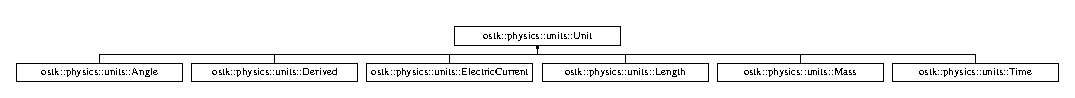
\includegraphics[height=0.868217cm]{classostk_1_1physics_1_1units_1_1_unit}
\end{center}
\end{figure}
\subsection*{Public Types}
\begin{DoxyCompactItemize}
\item 
enum \hyperlink{classostk_1_1physics_1_1units_1_1_unit_a113924e2dd880bd0e95d4ee9646ea4ca}{Type} \{ \newline
\hyperlink{classostk_1_1physics_1_1units_1_1_unit_a113924e2dd880bd0e95d4ee9646ea4caaec0fc0100c4fc1ce4eea230c3dc10360}{Type\+::\+Undefined}, 
\hyperlink{classostk_1_1physics_1_1units_1_1_unit_a113924e2dd880bd0e95d4ee9646ea4caaba2a9c6c8c77e03f83ef8bf543612275}{Type\+::\+Length}, 
\hyperlink{classostk_1_1physics_1_1units_1_1_unit_a113924e2dd880bd0e95d4ee9646ea4caaff2864d6f652ee0ac254814f1ae4f4a8}{Type\+::\+Mass}, 
\hyperlink{classostk_1_1physics_1_1units_1_1_unit_a113924e2dd880bd0e95d4ee9646ea4caaa76d4ef5f3f6a672bbfab2865563e530}{Type\+::\+Time}, 
\newline
\hyperlink{classostk_1_1physics_1_1units_1_1_unit_a113924e2dd880bd0e95d4ee9646ea4caaee7a8e262285ed49ea1b4e4ae11525bd}{Type\+::\+Temperature}, 
\hyperlink{classostk_1_1physics_1_1units_1_1_unit_a113924e2dd880bd0e95d4ee9646ea4caa9a60fd92ac6161bffa549ef2cd17f05e}{Type\+::\+Electric\+Current}, 
\hyperlink{classostk_1_1physics_1_1units_1_1_unit_a113924e2dd880bd0e95d4ee9646ea4caae91a9eb4f5dcc51ea18e180ea981d6ae}{Type\+::\+Luminous\+Intensity}, 
\hyperlink{classostk_1_1physics_1_1units_1_1_unit_a113924e2dd880bd0e95d4ee9646ea4caa0e77a10e9579997fa646fbda4118e108}{Type\+::\+Derived}
 \}
\end{DoxyCompactItemize}
\subsection*{Public Member Functions}
\begin{DoxyCompactItemize}
\item 
\hyperlink{classostk_1_1physics_1_1units_1_1_unit_a58e067b64c8ffbb58591c349cab49918}{Unit} (const \hyperlink{classostk_1_1physics_1_1units_1_1_unit_a113924e2dd880bd0e95d4ee9646ea4ca}{Unit\+::\+Type} \&a\+Type, const Real \&a\+Value)
\item 
virtual \hyperlink{classostk_1_1physics_1_1units_1_1_unit_ac2fa0cb556754667302d3585f5939789}{$\sim$\+Unit} ()=0
\item 
virtual \hyperlink{classostk_1_1physics_1_1units_1_1_unit}{Unit} $\ast$ \hyperlink{classostk_1_1physics_1_1units_1_1_unit_ab203628f8a16b16c28d89eaa4c3aff67}{clone} () const =0
\item 
bool \hyperlink{classostk_1_1physics_1_1units_1_1_unit_aa4f9685b3782e412db70a23f254f00b1}{operator==} (const \hyperlink{classostk_1_1physics_1_1units_1_1_unit}{Unit} \&a\+Unit) const
\item 
bool \hyperlink{classostk_1_1physics_1_1units_1_1_unit_a0a387db175de126d37d7375b7c4add64}{operator!=} (const \hyperlink{classostk_1_1physics_1_1units_1_1_unit}{Unit} \&a\+Unit) const
\item 
virtual bool \hyperlink{classostk_1_1physics_1_1units_1_1_unit_a423ce1df3478f0892b10824b591ae1cc}{is\+Defined} () const
\item 
bool \hyperlink{classostk_1_1physics_1_1units_1_1_unit_a75597249f1a5e3d0ed44769c23166cb6}{is\+Zero} () const
\item 
const Real \& \hyperlink{classostk_1_1physics_1_1units_1_1_unit_a85b5e9d502239f531903cac365abe78b}{access\+Value} () const
\item 
\hyperlink{classostk_1_1physics_1_1units_1_1_unit_a113924e2dd880bd0e95d4ee9646ea4ca}{Unit\+::\+Type} \hyperlink{classostk_1_1physics_1_1units_1_1_unit_aab2a8bd39d0294623a8be4bee9865aa2}{get\+Type} () const
\item 
Real \hyperlink{classostk_1_1physics_1_1units_1_1_unit_a0bfa6c131d5fb0bf1c4bd894ae84df17}{get\+Value} () const
\item 
virtual String \hyperlink{classostk_1_1physics_1_1units_1_1_unit_a8162b4eb8221c7577af16ab8b399d07e}{to\+String} (const Integer \&a\+Precision=Integer\+::\+Undefined()) const =0
\item 
Real \& \hyperlink{classostk_1_1physics_1_1units_1_1_unit_aed06dab6216e414fe22774debf200758}{access\+Value} ()
\item 
void \hyperlink{classostk_1_1physics_1_1units_1_1_unit_a51c95b69e4f83766aae377ba13d01f26}{set\+Value} (const Real \&a\+Value)
\end{DoxyCompactItemize}
\subsection*{Static Protected Member Functions}
\begin{DoxyCompactItemize}
\item 
static Pair$<$ Real, String $>$ \hyperlink{classostk_1_1physics_1_1units_1_1_unit_a3255171111d8c94390f6f87bbcb892ed}{Parse\+String} (const String \&a\+String)
\end{DoxyCompactItemize}


\subsection{Detailed Description}
\hyperlink{classostk_1_1physics_1_1units_1_1_unit}{Unit}. 

https\+://en.wikipedia.\+org/wiki/\+S\+I\+\_\+base\+\_\+unit

\begin{DoxyNote}{Note}
Could be (greatly) improved using templating... 

\href{https://benjaminjurke.com/content/articles/2015/compile-time-numerical-unit-dimension-checking/}{\tt https\+://benjaminjurke.\+com/content/articles/2015/compile-\/time-\/numerical-\/unit-\/dimension-\/checking/} 

\href{https://github.com/nholthaus/units}{\tt https\+://github.\+com/nholthaus/units} 

\href{https://www.boost.org/doc/libs/1_67_0/doc/html/boost_units.html}{\tt https\+://www.\+boost.\+org/doc/libs/1\+\_\+67\+\_\+0/doc/html/boost\+\_\+units.\+html} 
\end{DoxyNote}


\subsection{Member Enumeration Documentation}
\mbox{\Hypertarget{classostk_1_1physics_1_1units_1_1_unit_a113924e2dd880bd0e95d4ee9646ea4ca}\label{classostk_1_1physics_1_1units_1_1_unit_a113924e2dd880bd0e95d4ee9646ea4ca}} 
\index{ostk\+::physics\+::units\+::\+Unit@{ostk\+::physics\+::units\+::\+Unit}!Type@{Type}}
\index{Type@{Type}!ostk\+::physics\+::units\+::\+Unit@{ostk\+::physics\+::units\+::\+Unit}}
\subsubsection{\texorpdfstring{Type}{Type}}
{\footnotesize\ttfamily enum \hyperlink{classostk_1_1physics_1_1units_1_1_unit_a113924e2dd880bd0e95d4ee9646ea4ca}{ostk\+::physics\+::units\+::\+Unit\+::\+Type}\hspace{0.3cm}{\ttfamily [strong]}}

\begin{DoxyEnumFields}{Enumerator}
\raisebox{\heightof{T}}[0pt][0pt]{\index{Undefined@{Undefined}!ostk\+::physics\+::units\+::\+Unit@{ostk\+::physics\+::units\+::\+Unit}}\index{ostk\+::physics\+::units\+::\+Unit@{ostk\+::physics\+::units\+::\+Unit}!Undefined@{Undefined}}}\mbox{\Hypertarget{classostk_1_1physics_1_1units_1_1_unit_a113924e2dd880bd0e95d4ee9646ea4caaec0fc0100c4fc1ce4eea230c3dc10360}\label{classostk_1_1physics_1_1units_1_1_unit_a113924e2dd880bd0e95d4ee9646ea4caaec0fc0100c4fc1ce4eea230c3dc10360}} 
Undefined&\\
\hline

\raisebox{\heightof{T}}[0pt][0pt]{\index{Length@{Length}!ostk\+::physics\+::units\+::\+Unit@{ostk\+::physics\+::units\+::\+Unit}}\index{ostk\+::physics\+::units\+::\+Unit@{ostk\+::physics\+::units\+::\+Unit}!Length@{Length}}}\mbox{\Hypertarget{classostk_1_1physics_1_1units_1_1_unit_a113924e2dd880bd0e95d4ee9646ea4caaba2a9c6c8c77e03f83ef8bf543612275}\label{classostk_1_1physics_1_1units_1_1_unit_a113924e2dd880bd0e95d4ee9646ea4caaba2a9c6c8c77e03f83ef8bf543612275}} 
Length&\\
\hline

\raisebox{\heightof{T}}[0pt][0pt]{\index{Mass@{Mass}!ostk\+::physics\+::units\+::\+Unit@{ostk\+::physics\+::units\+::\+Unit}}\index{ostk\+::physics\+::units\+::\+Unit@{ostk\+::physics\+::units\+::\+Unit}!Mass@{Mass}}}\mbox{\Hypertarget{classostk_1_1physics_1_1units_1_1_unit_a113924e2dd880bd0e95d4ee9646ea4caaff2864d6f652ee0ac254814f1ae4f4a8}\label{classostk_1_1physics_1_1units_1_1_unit_a113924e2dd880bd0e95d4ee9646ea4caaff2864d6f652ee0ac254814f1ae4f4a8}} 
Mass&\\
\hline

\raisebox{\heightof{T}}[0pt][0pt]{\index{Time@{Time}!ostk\+::physics\+::units\+::\+Unit@{ostk\+::physics\+::units\+::\+Unit}}\index{ostk\+::physics\+::units\+::\+Unit@{ostk\+::physics\+::units\+::\+Unit}!Time@{Time}}}\mbox{\Hypertarget{classostk_1_1physics_1_1units_1_1_unit_a113924e2dd880bd0e95d4ee9646ea4caaa76d4ef5f3f6a672bbfab2865563e530}\label{classostk_1_1physics_1_1units_1_1_unit_a113924e2dd880bd0e95d4ee9646ea4caaa76d4ef5f3f6a672bbfab2865563e530}} 
Time&\\
\hline

\raisebox{\heightof{T}}[0pt][0pt]{\index{Temperature@{Temperature}!ostk\+::physics\+::units\+::\+Unit@{ostk\+::physics\+::units\+::\+Unit}}\index{ostk\+::physics\+::units\+::\+Unit@{ostk\+::physics\+::units\+::\+Unit}!Temperature@{Temperature}}}\mbox{\Hypertarget{classostk_1_1physics_1_1units_1_1_unit_a113924e2dd880bd0e95d4ee9646ea4caaee7a8e262285ed49ea1b4e4ae11525bd}\label{classostk_1_1physics_1_1units_1_1_unit_a113924e2dd880bd0e95d4ee9646ea4caaee7a8e262285ed49ea1b4e4ae11525bd}} 
Temperature&\\
\hline

\raisebox{\heightof{T}}[0pt][0pt]{\index{Electric\+Current@{Electric\+Current}!ostk\+::physics\+::units\+::\+Unit@{ostk\+::physics\+::units\+::\+Unit}}\index{ostk\+::physics\+::units\+::\+Unit@{ostk\+::physics\+::units\+::\+Unit}!Electric\+Current@{Electric\+Current}}}\mbox{\Hypertarget{classostk_1_1physics_1_1units_1_1_unit_a113924e2dd880bd0e95d4ee9646ea4caa9a60fd92ac6161bffa549ef2cd17f05e}\label{classostk_1_1physics_1_1units_1_1_unit_a113924e2dd880bd0e95d4ee9646ea4caa9a60fd92ac6161bffa549ef2cd17f05e}} 
Electric\+Current&\\
\hline

\raisebox{\heightof{T}}[0pt][0pt]{\index{Luminous\+Intensity@{Luminous\+Intensity}!ostk\+::physics\+::units\+::\+Unit@{ostk\+::physics\+::units\+::\+Unit}}\index{ostk\+::physics\+::units\+::\+Unit@{ostk\+::physics\+::units\+::\+Unit}!Luminous\+Intensity@{Luminous\+Intensity}}}\mbox{\Hypertarget{classostk_1_1physics_1_1units_1_1_unit_a113924e2dd880bd0e95d4ee9646ea4caae91a9eb4f5dcc51ea18e180ea981d6ae}\label{classostk_1_1physics_1_1units_1_1_unit_a113924e2dd880bd0e95d4ee9646ea4caae91a9eb4f5dcc51ea18e180ea981d6ae}} 
Luminous\+Intensity&\\
\hline

\raisebox{\heightof{T}}[0pt][0pt]{\index{Derived@{Derived}!ostk\+::physics\+::units\+::\+Unit@{ostk\+::physics\+::units\+::\+Unit}}\index{ostk\+::physics\+::units\+::\+Unit@{ostk\+::physics\+::units\+::\+Unit}!Derived@{Derived}}}\mbox{\Hypertarget{classostk_1_1physics_1_1units_1_1_unit_a113924e2dd880bd0e95d4ee9646ea4caa0e77a10e9579997fa646fbda4118e108}\label{classostk_1_1physics_1_1units_1_1_unit_a113924e2dd880bd0e95d4ee9646ea4caa0e77a10e9579997fa646fbda4118e108}} 
Derived&\\
\hline

\end{DoxyEnumFields}


\subsection{Constructor \& Destructor Documentation}
\mbox{\Hypertarget{classostk_1_1physics_1_1units_1_1_unit_a58e067b64c8ffbb58591c349cab49918}\label{classostk_1_1physics_1_1units_1_1_unit_a58e067b64c8ffbb58591c349cab49918}} 
\index{ostk\+::physics\+::units\+::\+Unit@{ostk\+::physics\+::units\+::\+Unit}!Unit@{Unit}}
\index{Unit@{Unit}!ostk\+::physics\+::units\+::\+Unit@{ostk\+::physics\+::units\+::\+Unit}}
\subsubsection{\texorpdfstring{Unit()}{Unit()}}
{\footnotesize\ttfamily ostk\+::physics\+::units\+::\+Unit\+::\+Unit (\begin{DoxyParamCaption}\item[{const \hyperlink{classostk_1_1physics_1_1units_1_1_unit_a113924e2dd880bd0e95d4ee9646ea4ca}{Unit\+::\+Type} \&}]{a\+Type,  }\item[{const Real \&}]{a\+Value }\end{DoxyParamCaption})}

\mbox{\Hypertarget{classostk_1_1physics_1_1units_1_1_unit_ac2fa0cb556754667302d3585f5939789}\label{classostk_1_1physics_1_1units_1_1_unit_ac2fa0cb556754667302d3585f5939789}} 
\index{ostk\+::physics\+::units\+::\+Unit@{ostk\+::physics\+::units\+::\+Unit}!````~Unit@{$\sim$\+Unit}}
\index{````~Unit@{$\sim$\+Unit}!ostk\+::physics\+::units\+::\+Unit@{ostk\+::physics\+::units\+::\+Unit}}
\subsubsection{\texorpdfstring{$\sim$\+Unit()}{~Unit()}}
{\footnotesize\ttfamily ostk\+::physics\+::units\+::\+Unit\+::$\sim$\+Unit (\begin{DoxyParamCaption}{ }\end{DoxyParamCaption})\hspace{0.3cm}{\ttfamily [pure virtual]}}



\subsection{Member Function Documentation}
\mbox{\Hypertarget{classostk_1_1physics_1_1units_1_1_unit_a85b5e9d502239f531903cac365abe78b}\label{classostk_1_1physics_1_1units_1_1_unit_a85b5e9d502239f531903cac365abe78b}} 
\index{ostk\+::physics\+::units\+::\+Unit@{ostk\+::physics\+::units\+::\+Unit}!access\+Value@{access\+Value}}
\index{access\+Value@{access\+Value}!ostk\+::physics\+::units\+::\+Unit@{ostk\+::physics\+::units\+::\+Unit}}
\subsubsection{\texorpdfstring{access\+Value()}{accessValue()}\hspace{0.1cm}{\footnotesize\ttfamily [1/2]}}
{\footnotesize\ttfamily const Real \& ostk\+::physics\+::units\+::\+Unit\+::access\+Value (\begin{DoxyParamCaption}{ }\end{DoxyParamCaption}) const}

\mbox{\Hypertarget{classostk_1_1physics_1_1units_1_1_unit_aed06dab6216e414fe22774debf200758}\label{classostk_1_1physics_1_1units_1_1_unit_aed06dab6216e414fe22774debf200758}} 
\index{ostk\+::physics\+::units\+::\+Unit@{ostk\+::physics\+::units\+::\+Unit}!access\+Value@{access\+Value}}
\index{access\+Value@{access\+Value}!ostk\+::physics\+::units\+::\+Unit@{ostk\+::physics\+::units\+::\+Unit}}
\subsubsection{\texorpdfstring{access\+Value()}{accessValue()}\hspace{0.1cm}{\footnotesize\ttfamily [2/2]}}
{\footnotesize\ttfamily Real \& ostk\+::physics\+::units\+::\+Unit\+::access\+Value (\begin{DoxyParamCaption}{ }\end{DoxyParamCaption})}

\mbox{\Hypertarget{classostk_1_1physics_1_1units_1_1_unit_ab203628f8a16b16c28d89eaa4c3aff67}\label{classostk_1_1physics_1_1units_1_1_unit_ab203628f8a16b16c28d89eaa4c3aff67}} 
\index{ostk\+::physics\+::units\+::\+Unit@{ostk\+::physics\+::units\+::\+Unit}!clone@{clone}}
\index{clone@{clone}!ostk\+::physics\+::units\+::\+Unit@{ostk\+::physics\+::units\+::\+Unit}}
\subsubsection{\texorpdfstring{clone()}{clone()}}
{\footnotesize\ttfamily virtual \hyperlink{classostk_1_1physics_1_1units_1_1_unit}{Unit}$\ast$ ostk\+::physics\+::units\+::\+Unit\+::clone (\begin{DoxyParamCaption}{ }\end{DoxyParamCaption}) const\hspace{0.3cm}{\ttfamily [pure virtual]}}



Implemented in \hyperlink{classostk_1_1physics_1_1units_1_1_derived_a72a1ae09398204d52a9078da6d36d9d7}{ostk\+::physics\+::units\+::\+Derived}, \hyperlink{classostk_1_1physics_1_1units_1_1_angle_af0d5d649b2a1310e6337663f7b9283bf}{ostk\+::physics\+::units\+::\+Angle}, \hyperlink{classostk_1_1physics_1_1units_1_1_time_ae714d9f44d7ab651de5f37c5085f38fa}{ostk\+::physics\+::units\+::\+Time}, \hyperlink{classostk_1_1physics_1_1units_1_1_length_aeeb9cf27e0ea9bd818ad806cf3083658}{ostk\+::physics\+::units\+::\+Length}, \hyperlink{classostk_1_1physics_1_1units_1_1_mass_a1466c0c4860d94b0e6630476d4216033}{ostk\+::physics\+::units\+::\+Mass}, and \hyperlink{classostk_1_1physics_1_1units_1_1_electric_current_ac8a261411dee39c74bc43201e8e9c9dd}{ostk\+::physics\+::units\+::\+Electric\+Current}.

\mbox{\Hypertarget{classostk_1_1physics_1_1units_1_1_unit_aab2a8bd39d0294623a8be4bee9865aa2}\label{classostk_1_1physics_1_1units_1_1_unit_aab2a8bd39d0294623a8be4bee9865aa2}} 
\index{ostk\+::physics\+::units\+::\+Unit@{ostk\+::physics\+::units\+::\+Unit}!get\+Type@{get\+Type}}
\index{get\+Type@{get\+Type}!ostk\+::physics\+::units\+::\+Unit@{ostk\+::physics\+::units\+::\+Unit}}
\subsubsection{\texorpdfstring{get\+Type()}{getType()}}
{\footnotesize\ttfamily \hyperlink{classostk_1_1physics_1_1units_1_1_unit_a113924e2dd880bd0e95d4ee9646ea4ca}{Unit\+::\+Type} ostk\+::physics\+::units\+::\+Unit\+::get\+Type (\begin{DoxyParamCaption}{ }\end{DoxyParamCaption}) const}

\mbox{\Hypertarget{classostk_1_1physics_1_1units_1_1_unit_a0bfa6c131d5fb0bf1c4bd894ae84df17}\label{classostk_1_1physics_1_1units_1_1_unit_a0bfa6c131d5fb0bf1c4bd894ae84df17}} 
\index{ostk\+::physics\+::units\+::\+Unit@{ostk\+::physics\+::units\+::\+Unit}!get\+Value@{get\+Value}}
\index{get\+Value@{get\+Value}!ostk\+::physics\+::units\+::\+Unit@{ostk\+::physics\+::units\+::\+Unit}}
\subsubsection{\texorpdfstring{get\+Value()}{getValue()}}
{\footnotesize\ttfamily Real ostk\+::physics\+::units\+::\+Unit\+::get\+Value (\begin{DoxyParamCaption}{ }\end{DoxyParamCaption}) const}

\mbox{\Hypertarget{classostk_1_1physics_1_1units_1_1_unit_a423ce1df3478f0892b10824b591ae1cc}\label{classostk_1_1physics_1_1units_1_1_unit_a423ce1df3478f0892b10824b591ae1cc}} 
\index{ostk\+::physics\+::units\+::\+Unit@{ostk\+::physics\+::units\+::\+Unit}!is\+Defined@{is\+Defined}}
\index{is\+Defined@{is\+Defined}!ostk\+::physics\+::units\+::\+Unit@{ostk\+::physics\+::units\+::\+Unit}}
\subsubsection{\texorpdfstring{is\+Defined()}{isDefined()}}
{\footnotesize\ttfamily bool ostk\+::physics\+::units\+::\+Unit\+::is\+Defined (\begin{DoxyParamCaption}{ }\end{DoxyParamCaption}) const\hspace{0.3cm}{\ttfamily [virtual]}}



Reimplemented in \hyperlink{classostk_1_1physics_1_1units_1_1_derived_a4221766463c2f4ab478e4a882239eec6}{ostk\+::physics\+::units\+::\+Derived}, \hyperlink{classostk_1_1physics_1_1units_1_1_angle_a912562d12513b2fcee56262208206b62}{ostk\+::physics\+::units\+::\+Angle}, \hyperlink{classostk_1_1physics_1_1units_1_1_length_aa176a675943dfe488fe96005c5405304}{ostk\+::physics\+::units\+::\+Length}, \hyperlink{classostk_1_1physics_1_1units_1_1_time_a1b89925067e81636fa80f6e73eed3625}{ostk\+::physics\+::units\+::\+Time}, \hyperlink{classostk_1_1physics_1_1units_1_1_mass_ad6bb821365eff3a414d9fd07a7730d99}{ostk\+::physics\+::units\+::\+Mass}, and \hyperlink{classostk_1_1physics_1_1units_1_1_electric_current_a81ae490a737a49553a7c390b865486a7}{ostk\+::physics\+::units\+::\+Electric\+Current}.

\mbox{\Hypertarget{classostk_1_1physics_1_1units_1_1_unit_a75597249f1a5e3d0ed44769c23166cb6}\label{classostk_1_1physics_1_1units_1_1_unit_a75597249f1a5e3d0ed44769c23166cb6}} 
\index{ostk\+::physics\+::units\+::\+Unit@{ostk\+::physics\+::units\+::\+Unit}!is\+Zero@{is\+Zero}}
\index{is\+Zero@{is\+Zero}!ostk\+::physics\+::units\+::\+Unit@{ostk\+::physics\+::units\+::\+Unit}}
\subsubsection{\texorpdfstring{is\+Zero()}{isZero()}}
{\footnotesize\ttfamily bool ostk\+::physics\+::units\+::\+Unit\+::is\+Zero (\begin{DoxyParamCaption}{ }\end{DoxyParamCaption}) const}

\mbox{\Hypertarget{classostk_1_1physics_1_1units_1_1_unit_a0a387db175de126d37d7375b7c4add64}\label{classostk_1_1physics_1_1units_1_1_unit_a0a387db175de126d37d7375b7c4add64}} 
\index{ostk\+::physics\+::units\+::\+Unit@{ostk\+::physics\+::units\+::\+Unit}!operator"!=@{operator"!=}}
\index{operator"!=@{operator"!=}!ostk\+::physics\+::units\+::\+Unit@{ostk\+::physics\+::units\+::\+Unit}}
\subsubsection{\texorpdfstring{operator"!=()}{operator!=()}}
{\footnotesize\ttfamily bool ostk\+::physics\+::units\+::\+Unit\+::operator!= (\begin{DoxyParamCaption}\item[{const \hyperlink{classostk_1_1physics_1_1units_1_1_unit}{Unit} \&}]{a\+Unit }\end{DoxyParamCaption}) const}

\mbox{\Hypertarget{classostk_1_1physics_1_1units_1_1_unit_aa4f9685b3782e412db70a23f254f00b1}\label{classostk_1_1physics_1_1units_1_1_unit_aa4f9685b3782e412db70a23f254f00b1}} 
\index{ostk\+::physics\+::units\+::\+Unit@{ostk\+::physics\+::units\+::\+Unit}!operator==@{operator==}}
\index{operator==@{operator==}!ostk\+::physics\+::units\+::\+Unit@{ostk\+::physics\+::units\+::\+Unit}}
\subsubsection{\texorpdfstring{operator==()}{operator==()}}
{\footnotesize\ttfamily bool ostk\+::physics\+::units\+::\+Unit\+::operator== (\begin{DoxyParamCaption}\item[{const \hyperlink{classostk_1_1physics_1_1units_1_1_unit}{Unit} \&}]{a\+Unit }\end{DoxyParamCaption}) const}

\mbox{\Hypertarget{classostk_1_1physics_1_1units_1_1_unit_a3255171111d8c94390f6f87bbcb892ed}\label{classostk_1_1physics_1_1units_1_1_unit_a3255171111d8c94390f6f87bbcb892ed}} 
\index{ostk\+::physics\+::units\+::\+Unit@{ostk\+::physics\+::units\+::\+Unit}!Parse\+String@{Parse\+String}}
\index{Parse\+String@{Parse\+String}!ostk\+::physics\+::units\+::\+Unit@{ostk\+::physics\+::units\+::\+Unit}}
\subsubsection{\texorpdfstring{Parse\+String()}{ParseString()}}
{\footnotesize\ttfamily Pair$<$ Real, String $>$ ostk\+::physics\+::units\+::\+Unit\+::\+Parse\+String (\begin{DoxyParamCaption}\item[{const String \&}]{a\+String }\end{DoxyParamCaption})\hspace{0.3cm}{\ttfamily [static]}, {\ttfamily [protected]}}

\mbox{\Hypertarget{classostk_1_1physics_1_1units_1_1_unit_a51c95b69e4f83766aae377ba13d01f26}\label{classostk_1_1physics_1_1units_1_1_unit_a51c95b69e4f83766aae377ba13d01f26}} 
\index{ostk\+::physics\+::units\+::\+Unit@{ostk\+::physics\+::units\+::\+Unit}!set\+Value@{set\+Value}}
\index{set\+Value@{set\+Value}!ostk\+::physics\+::units\+::\+Unit@{ostk\+::physics\+::units\+::\+Unit}}
\subsubsection{\texorpdfstring{set\+Value()}{setValue()}}
{\footnotesize\ttfamily void ostk\+::physics\+::units\+::\+Unit\+::set\+Value (\begin{DoxyParamCaption}\item[{const Real \&}]{a\+Value }\end{DoxyParamCaption})}

\mbox{\Hypertarget{classostk_1_1physics_1_1units_1_1_unit_a8162b4eb8221c7577af16ab8b399d07e}\label{classostk_1_1physics_1_1units_1_1_unit_a8162b4eb8221c7577af16ab8b399d07e}} 
\index{ostk\+::physics\+::units\+::\+Unit@{ostk\+::physics\+::units\+::\+Unit}!to\+String@{to\+String}}
\index{to\+String@{to\+String}!ostk\+::physics\+::units\+::\+Unit@{ostk\+::physics\+::units\+::\+Unit}}
\subsubsection{\texorpdfstring{to\+String()}{toString()}}
{\footnotesize\ttfamily virtual String ostk\+::physics\+::units\+::\+Unit\+::to\+String (\begin{DoxyParamCaption}\item[{const Integer \&}]{a\+Precision = {\ttfamily Integer\+:\+:Undefined()} }\end{DoxyParamCaption}) const\hspace{0.3cm}{\ttfamily [pure virtual]}}



Implemented in \hyperlink{classostk_1_1physics_1_1units_1_1_derived_ac1794677978fba5582fb127e032f7398}{ostk\+::physics\+::units\+::\+Derived}, \hyperlink{classostk_1_1physics_1_1units_1_1_angle_a7403146e01d293dfdd30130f9a9f0f2f}{ostk\+::physics\+::units\+::\+Angle}, \hyperlink{classostk_1_1physics_1_1units_1_1_length_ad3ec518939d2ffc86cd73b8ed4c071af}{ostk\+::physics\+::units\+::\+Length}, \hyperlink{classostk_1_1physics_1_1units_1_1_time_a6805d7d9b298d1ba9f219294e11a363c}{ostk\+::physics\+::units\+::\+Time}, \hyperlink{classostk_1_1physics_1_1units_1_1_mass_aa8993fb7d2dbed494bbb68f8ec002af5}{ostk\+::physics\+::units\+::\+Mass}, and \hyperlink{classostk_1_1physics_1_1units_1_1_electric_current_aa720f442c93f18f81ad769edbd570bd5}{ostk\+::physics\+::units\+::\+Electric\+Current}.



The documentation for this class was generated from the following files\+:\begin{DoxyCompactItemize}
\item 
include/\+Open\+Space\+Toolkit/\+Physics/\+Units/\hyperlink{_units_2_unit_8hpp}{Unit.\+hpp}\item 
src/\+Open\+Space\+Toolkit/\+Physics/\+Units/\hyperlink{_units_2_unit_8cpp}{Unit.\+cpp}\end{DoxyCompactItemize}

\hypertarget{classostk_1_1physics_1_1_unit}{}\section{ostk\+:\+:physics\+:\+:Unit Class Reference}
\label{classostk_1_1physics_1_1_unit}\index{ostk\+::physics\+::\+Unit@{ostk\+::physics\+::\+Unit}}


\hyperlink{classostk_1_1physics_1_1_unit}{Unit}.  




{\ttfamily \#include $<$Unit.\+hpp$>$}

\subsection*{Public Types}
\begin{DoxyCompactItemize}
\item 
enum \hyperlink{classostk_1_1physics_1_1_unit_a1c07d36cd02be8541eb972367e2b628f}{Type} \{ \newline
\hyperlink{classostk_1_1physics_1_1_unit_a1c07d36cd02be8541eb972367e2b628faec0fc0100c4fc1ce4eea230c3dc10360}{Type\+::\+Undefined}, 
\hyperlink{classostk_1_1physics_1_1_unit_a1c07d36cd02be8541eb972367e2b628fa6adf97f83acf6453d4a6a4b1070f3754}{Type\+::\+None}, 
\hyperlink{classostk_1_1physics_1_1_unit_a1c07d36cd02be8541eb972367e2b628faba2a9c6c8c77e03f83ef8bf543612275}{Type\+::\+Length}, 
\hyperlink{classostk_1_1physics_1_1_unit_a1c07d36cd02be8541eb972367e2b628faff2864d6f652ee0ac254814f1ae4f4a8}{Type\+::\+Mass}, 
\newline
\hyperlink{classostk_1_1physics_1_1_unit_a1c07d36cd02be8541eb972367e2b628faa76d4ef5f3f6a672bbfab2865563e530}{Type\+::\+Time}, 
\hyperlink{classostk_1_1physics_1_1_unit_a1c07d36cd02be8541eb972367e2b628faee7a8e262285ed49ea1b4e4ae11525bd}{Type\+::\+Temperature}, 
\hyperlink{classostk_1_1physics_1_1_unit_a1c07d36cd02be8541eb972367e2b628fa9a60fd92ac6161bffa549ef2cd17f05e}{Type\+::\+Electric\+Current}, 
\hyperlink{classostk_1_1physics_1_1_unit_a1c07d36cd02be8541eb972367e2b628fae91a9eb4f5dcc51ea18e180ea981d6ae}{Type\+::\+Luminous\+Intensity}, 
\newline
\hyperlink{classostk_1_1physics_1_1_unit_a1c07d36cd02be8541eb972367e2b628fa0e77a10e9579997fa646fbda4118e108}{Type\+::\+Derived}
 \}
\end{DoxyCompactItemize}
\subsection*{Public Member Functions}
\begin{DoxyCompactItemize}
\item 
\hyperlink{classostk_1_1physics_1_1_unit_abb6ab5ed9dcc07c65af5bb594e5f87f0}{Unit} ()=delete
\item 
\hyperlink{classostk_1_1physics_1_1_unit_aaa79239cad3b8499ce9dc4ebec2b8f05}{Unit} (const \hyperlink{classostk_1_1physics_1_1_unit}{Unit} \&a\+Unit)
\item 
\hyperlink{classostk_1_1physics_1_1_unit}{Unit} \& \hyperlink{classostk_1_1physics_1_1_unit_a1ca37a2c58beea2b837504356ac9a312}{operator=} (const \hyperlink{classostk_1_1physics_1_1_unit}{Unit} \&a\+Unit)
\item 
bool \hyperlink{classostk_1_1physics_1_1_unit_a2f402b7601cef9914f8c367e44f9886c}{operator==} (const \hyperlink{classostk_1_1physics_1_1_unit}{Unit} \&a\+Unit) const
\item 
bool \hyperlink{classostk_1_1physics_1_1_unit_ab99c2e4afec3e69ba573528dd9f3f9ac}{operator!=} (const \hyperlink{classostk_1_1physics_1_1_unit}{Unit} \&a\+Unit) const
\item 
bool \hyperlink{classostk_1_1physics_1_1_unit_a94e73e5bae82b568280fd3055702dac8}{is\+Defined} () const
\item 
bool \hyperlink{classostk_1_1physics_1_1_unit_a300c6c5aac22fa2badf2b8a480d770f8}{is\+None} () const
\item 
\hyperlink{classostk_1_1physics_1_1_unit_a1c07d36cd02be8541eb972367e2b628f}{Unit\+::\+Type} \hyperlink{classostk_1_1physics_1_1_unit_ad7cf872fcf44faaa79b4f59855060f89}{get\+Type} () const
\item 
Real \hyperlink{classostk_1_1physics_1_1_unit_a6c88c955a56b590f4623e8a1fa2a9cbb}{ratio\+To} (const \hyperlink{classostk_1_1physics_1_1_unit}{Unit} \&a\+Unit) const
\item 
String \hyperlink{classostk_1_1physics_1_1_unit_a496115fe0905a2a26b6f742382f3b7f0}{to\+String} () const
\end{DoxyCompactItemize}
\subsection*{Static Public Member Functions}
\begin{DoxyCompactItemize}
\item 
static \hyperlink{classostk_1_1physics_1_1_unit}{Unit} \hyperlink{classostk_1_1physics_1_1_unit_a61c8e231a744ece53683ae79deee0850}{Undefined} ()
\item 
static \hyperlink{classostk_1_1physics_1_1_unit}{Unit} \hyperlink{classostk_1_1physics_1_1_unit_a72a993421e48c8b2d4d4fd89ce0142da}{None} ()
\item 
static \hyperlink{classostk_1_1physics_1_1_unit}{Unit} \hyperlink{classostk_1_1physics_1_1_unit_abbf99c91d09a31011c18b359c49d31ed}{Length} (const \hyperlink{classostk_1_1physics_1_1units_1_1_length_a2664470a7eedf5d45c88861fe69badea}{units\+::\+Length\+::\+Unit} \&a\+Length\+Unit)
\item 
static \hyperlink{classostk_1_1physics_1_1_unit}{Unit} \hyperlink{classostk_1_1physics_1_1_unit_af41e733d436f73949ab2fd9766071bdd}{Derived} (const \hyperlink{classostk_1_1physics_1_1units_1_1_derived_1_1_unit}{units\+::\+Derived\+::\+Unit} \&a\+Derived\+Unit)
\item 
static String \hyperlink{classostk_1_1physics_1_1_unit_a2834e4e5fa10d96212016a3cb8a02f02}{String\+From\+Type} (const \hyperlink{classostk_1_1physics_1_1_unit_a1c07d36cd02be8541eb972367e2b628f}{Unit\+::\+Type} \&a\+Type)
\end{DoxyCompactItemize}
\subsection*{Friends}
\begin{DoxyCompactItemize}
\item 
std\+::ostream \& \hyperlink{classostk_1_1physics_1_1_unit_a70630a82d569152709a999efabdb3e4f}{operator$<$$<$} (std\+::ostream \&an\+Output\+Stream, const \hyperlink{classostk_1_1physics_1_1_unit}{Unit} \&a\+Unit)
\end{DoxyCompactItemize}


\subsection{Detailed Description}
\hyperlink{classostk_1_1physics_1_1_unit}{Unit}. 

A unit of measurement is a definite magnitude of a quantity, defined and adopted by convention or by law, that is used as a standard for measurement of the same kind of quantity. Any other quantity of that kind can be expressed as a multiple of the unit of measurement.

https\+://en.wikipedia.\+org/wiki/\+Unit\+\_\+of\+\_\+measurement 

\subsection{Member Enumeration Documentation}
\mbox{\Hypertarget{classostk_1_1physics_1_1_unit_a1c07d36cd02be8541eb972367e2b628f}\label{classostk_1_1physics_1_1_unit_a1c07d36cd02be8541eb972367e2b628f}} 
\index{ostk\+::physics\+::\+Unit@{ostk\+::physics\+::\+Unit}!Type@{Type}}
\index{Type@{Type}!ostk\+::physics\+::\+Unit@{ostk\+::physics\+::\+Unit}}
\subsubsection{\texorpdfstring{Type}{Type}}
{\footnotesize\ttfamily enum \hyperlink{classostk_1_1physics_1_1_unit_a1c07d36cd02be8541eb972367e2b628f}{ostk\+::physics\+::\+Unit\+::\+Type}\hspace{0.3cm}{\ttfamily [strong]}}

\begin{DoxyEnumFields}{Enumerator}
\raisebox{\heightof{T}}[0pt][0pt]{\index{Undefined@{Undefined}!ostk\+::physics\+::\+Unit@{ostk\+::physics\+::\+Unit}}\index{ostk\+::physics\+::\+Unit@{ostk\+::physics\+::\+Unit}!Undefined@{Undefined}}}\mbox{\Hypertarget{classostk_1_1physics_1_1_unit_a1c07d36cd02be8541eb972367e2b628faec0fc0100c4fc1ce4eea230c3dc10360}\label{classostk_1_1physics_1_1_unit_a1c07d36cd02be8541eb972367e2b628faec0fc0100c4fc1ce4eea230c3dc10360}} 
Undefined&\\
\hline

\raisebox{\heightof{T}}[0pt][0pt]{\index{None@{None}!ostk\+::physics\+::\+Unit@{ostk\+::physics\+::\+Unit}}\index{ostk\+::physics\+::\+Unit@{ostk\+::physics\+::\+Unit}!None@{None}}}\mbox{\Hypertarget{classostk_1_1physics_1_1_unit_a1c07d36cd02be8541eb972367e2b628fa6adf97f83acf6453d4a6a4b1070f3754}\label{classostk_1_1physics_1_1_unit_a1c07d36cd02be8541eb972367e2b628fa6adf97f83acf6453d4a6a4b1070f3754}} 
None&\\
\hline

\raisebox{\heightof{T}}[0pt][0pt]{\index{Length@{Length}!ostk\+::physics\+::\+Unit@{ostk\+::physics\+::\+Unit}}\index{ostk\+::physics\+::\+Unit@{ostk\+::physics\+::\+Unit}!Length@{Length}}}\mbox{\Hypertarget{classostk_1_1physics_1_1_unit_a1c07d36cd02be8541eb972367e2b628faba2a9c6c8c77e03f83ef8bf543612275}\label{classostk_1_1physics_1_1_unit_a1c07d36cd02be8541eb972367e2b628faba2a9c6c8c77e03f83ef8bf543612275}} 
Length&\\
\hline

\raisebox{\heightof{T}}[0pt][0pt]{\index{Mass@{Mass}!ostk\+::physics\+::\+Unit@{ostk\+::physics\+::\+Unit}}\index{ostk\+::physics\+::\+Unit@{ostk\+::physics\+::\+Unit}!Mass@{Mass}}}\mbox{\Hypertarget{classostk_1_1physics_1_1_unit_a1c07d36cd02be8541eb972367e2b628faff2864d6f652ee0ac254814f1ae4f4a8}\label{classostk_1_1physics_1_1_unit_a1c07d36cd02be8541eb972367e2b628faff2864d6f652ee0ac254814f1ae4f4a8}} 
Mass&\\
\hline

\raisebox{\heightof{T}}[0pt][0pt]{\index{Time@{Time}!ostk\+::physics\+::\+Unit@{ostk\+::physics\+::\+Unit}}\index{ostk\+::physics\+::\+Unit@{ostk\+::physics\+::\+Unit}!Time@{Time}}}\mbox{\Hypertarget{classostk_1_1physics_1_1_unit_a1c07d36cd02be8541eb972367e2b628faa76d4ef5f3f6a672bbfab2865563e530}\label{classostk_1_1physics_1_1_unit_a1c07d36cd02be8541eb972367e2b628faa76d4ef5f3f6a672bbfab2865563e530}} 
Time&\\
\hline

\raisebox{\heightof{T}}[0pt][0pt]{\index{Temperature@{Temperature}!ostk\+::physics\+::\+Unit@{ostk\+::physics\+::\+Unit}}\index{ostk\+::physics\+::\+Unit@{ostk\+::physics\+::\+Unit}!Temperature@{Temperature}}}\mbox{\Hypertarget{classostk_1_1physics_1_1_unit_a1c07d36cd02be8541eb972367e2b628faee7a8e262285ed49ea1b4e4ae11525bd}\label{classostk_1_1physics_1_1_unit_a1c07d36cd02be8541eb972367e2b628faee7a8e262285ed49ea1b4e4ae11525bd}} 
Temperature&\\
\hline

\raisebox{\heightof{T}}[0pt][0pt]{\index{Electric\+Current@{Electric\+Current}!ostk\+::physics\+::\+Unit@{ostk\+::physics\+::\+Unit}}\index{ostk\+::physics\+::\+Unit@{ostk\+::physics\+::\+Unit}!Electric\+Current@{Electric\+Current}}}\mbox{\Hypertarget{classostk_1_1physics_1_1_unit_a1c07d36cd02be8541eb972367e2b628fa9a60fd92ac6161bffa549ef2cd17f05e}\label{classostk_1_1physics_1_1_unit_a1c07d36cd02be8541eb972367e2b628fa9a60fd92ac6161bffa549ef2cd17f05e}} 
Electric\+Current&\\
\hline

\raisebox{\heightof{T}}[0pt][0pt]{\index{Luminous\+Intensity@{Luminous\+Intensity}!ostk\+::physics\+::\+Unit@{ostk\+::physics\+::\+Unit}}\index{ostk\+::physics\+::\+Unit@{ostk\+::physics\+::\+Unit}!Luminous\+Intensity@{Luminous\+Intensity}}}\mbox{\Hypertarget{classostk_1_1physics_1_1_unit_a1c07d36cd02be8541eb972367e2b628fae91a9eb4f5dcc51ea18e180ea981d6ae}\label{classostk_1_1physics_1_1_unit_a1c07d36cd02be8541eb972367e2b628fae91a9eb4f5dcc51ea18e180ea981d6ae}} 
Luminous\+Intensity&\\
\hline

\raisebox{\heightof{T}}[0pt][0pt]{\index{Derived@{Derived}!ostk\+::physics\+::\+Unit@{ostk\+::physics\+::\+Unit}}\index{ostk\+::physics\+::\+Unit@{ostk\+::physics\+::\+Unit}!Derived@{Derived}}}\mbox{\Hypertarget{classostk_1_1physics_1_1_unit_a1c07d36cd02be8541eb972367e2b628fa0e77a10e9579997fa646fbda4118e108}\label{classostk_1_1physics_1_1_unit_a1c07d36cd02be8541eb972367e2b628fa0e77a10e9579997fa646fbda4118e108}} 
Derived&\\
\hline

\end{DoxyEnumFields}


\subsection{Constructor \& Destructor Documentation}
\mbox{\Hypertarget{classostk_1_1physics_1_1_unit_abb6ab5ed9dcc07c65af5bb594e5f87f0}\label{classostk_1_1physics_1_1_unit_abb6ab5ed9dcc07c65af5bb594e5f87f0}} 
\index{ostk\+::physics\+::\+Unit@{ostk\+::physics\+::\+Unit}!Unit@{Unit}}
\index{Unit@{Unit}!ostk\+::physics\+::\+Unit@{ostk\+::physics\+::\+Unit}}
\subsubsection{\texorpdfstring{Unit()}{Unit()}\hspace{0.1cm}{\footnotesize\ttfamily [1/2]}}
{\footnotesize\ttfamily ostk\+::physics\+::\+Unit\+::\+Unit (\begin{DoxyParamCaption}{ }\end{DoxyParamCaption})\hspace{0.3cm}{\ttfamily [delete]}}

\mbox{\Hypertarget{classostk_1_1physics_1_1_unit_aaa79239cad3b8499ce9dc4ebec2b8f05}\label{classostk_1_1physics_1_1_unit_aaa79239cad3b8499ce9dc4ebec2b8f05}} 
\index{ostk\+::physics\+::\+Unit@{ostk\+::physics\+::\+Unit}!Unit@{Unit}}
\index{Unit@{Unit}!ostk\+::physics\+::\+Unit@{ostk\+::physics\+::\+Unit}}
\subsubsection{\texorpdfstring{Unit()}{Unit()}\hspace{0.1cm}{\footnotesize\ttfamily [2/2]}}
{\footnotesize\ttfamily ostk\+::physics\+::\+Unit\+::\+Unit (\begin{DoxyParamCaption}\item[{const \hyperlink{classostk_1_1physics_1_1_unit}{Unit} \&}]{a\+Unit }\end{DoxyParamCaption})}



\subsection{Member Function Documentation}
\mbox{\Hypertarget{classostk_1_1physics_1_1_unit_af41e733d436f73949ab2fd9766071bdd}\label{classostk_1_1physics_1_1_unit_af41e733d436f73949ab2fd9766071bdd}} 
\index{ostk\+::physics\+::\+Unit@{ostk\+::physics\+::\+Unit}!Derived@{Derived}}
\index{Derived@{Derived}!ostk\+::physics\+::\+Unit@{ostk\+::physics\+::\+Unit}}
\subsubsection{\texorpdfstring{Derived()}{Derived()}}
{\footnotesize\ttfamily \hyperlink{classostk_1_1physics_1_1_unit}{Unit} ostk\+::physics\+::\+Unit\+::\+Derived (\begin{DoxyParamCaption}\item[{const \hyperlink{classostk_1_1physics_1_1units_1_1_derived_1_1_unit}{units\+::\+Derived\+::\+Unit} \&}]{a\+Derived\+Unit }\end{DoxyParamCaption})\hspace{0.3cm}{\ttfamily [static]}}

\mbox{\Hypertarget{classostk_1_1physics_1_1_unit_ad7cf872fcf44faaa79b4f59855060f89}\label{classostk_1_1physics_1_1_unit_ad7cf872fcf44faaa79b4f59855060f89}} 
\index{ostk\+::physics\+::\+Unit@{ostk\+::physics\+::\+Unit}!get\+Type@{get\+Type}}
\index{get\+Type@{get\+Type}!ostk\+::physics\+::\+Unit@{ostk\+::physics\+::\+Unit}}
\subsubsection{\texorpdfstring{get\+Type()}{getType()}}
{\footnotesize\ttfamily \hyperlink{classostk_1_1physics_1_1_unit_a1c07d36cd02be8541eb972367e2b628f}{Unit\+::\+Type} ostk\+::physics\+::\+Unit\+::get\+Type (\begin{DoxyParamCaption}{ }\end{DoxyParamCaption}) const}

\mbox{\Hypertarget{classostk_1_1physics_1_1_unit_a94e73e5bae82b568280fd3055702dac8}\label{classostk_1_1physics_1_1_unit_a94e73e5bae82b568280fd3055702dac8}} 
\index{ostk\+::physics\+::\+Unit@{ostk\+::physics\+::\+Unit}!is\+Defined@{is\+Defined}}
\index{is\+Defined@{is\+Defined}!ostk\+::physics\+::\+Unit@{ostk\+::physics\+::\+Unit}}
\subsubsection{\texorpdfstring{is\+Defined()}{isDefined()}}
{\footnotesize\ttfamily bool ostk\+::physics\+::\+Unit\+::is\+Defined (\begin{DoxyParamCaption}{ }\end{DoxyParamCaption}) const}

\mbox{\Hypertarget{classostk_1_1physics_1_1_unit_a300c6c5aac22fa2badf2b8a480d770f8}\label{classostk_1_1physics_1_1_unit_a300c6c5aac22fa2badf2b8a480d770f8}} 
\index{ostk\+::physics\+::\+Unit@{ostk\+::physics\+::\+Unit}!is\+None@{is\+None}}
\index{is\+None@{is\+None}!ostk\+::physics\+::\+Unit@{ostk\+::physics\+::\+Unit}}
\subsubsection{\texorpdfstring{is\+None()}{isNone()}}
{\footnotesize\ttfamily bool ostk\+::physics\+::\+Unit\+::is\+None (\begin{DoxyParamCaption}{ }\end{DoxyParamCaption}) const}

\mbox{\Hypertarget{classostk_1_1physics_1_1_unit_abbf99c91d09a31011c18b359c49d31ed}\label{classostk_1_1physics_1_1_unit_abbf99c91d09a31011c18b359c49d31ed}} 
\index{ostk\+::physics\+::\+Unit@{ostk\+::physics\+::\+Unit}!Length@{Length}}
\index{Length@{Length}!ostk\+::physics\+::\+Unit@{ostk\+::physics\+::\+Unit}}
\subsubsection{\texorpdfstring{Length()}{Length()}}
{\footnotesize\ttfamily \hyperlink{classostk_1_1physics_1_1_unit}{Unit} ostk\+::physics\+::\+Unit\+::\+Length (\begin{DoxyParamCaption}\item[{const \hyperlink{classostk_1_1physics_1_1units_1_1_length_a2664470a7eedf5d45c88861fe69badea}{units\+::\+Length\+::\+Unit} \&}]{a\+Length\+Unit }\end{DoxyParamCaption})\hspace{0.3cm}{\ttfamily [static]}}

\mbox{\Hypertarget{classostk_1_1physics_1_1_unit_a72a993421e48c8b2d4d4fd89ce0142da}\label{classostk_1_1physics_1_1_unit_a72a993421e48c8b2d4d4fd89ce0142da}} 
\index{ostk\+::physics\+::\+Unit@{ostk\+::physics\+::\+Unit}!None@{None}}
\index{None@{None}!ostk\+::physics\+::\+Unit@{ostk\+::physics\+::\+Unit}}
\subsubsection{\texorpdfstring{None()}{None()}}
{\footnotesize\ttfamily \hyperlink{classostk_1_1physics_1_1_unit}{Unit} ostk\+::physics\+::\+Unit\+::\+None (\begin{DoxyParamCaption}{ }\end{DoxyParamCaption})\hspace{0.3cm}{\ttfamily [static]}}

\mbox{\Hypertarget{classostk_1_1physics_1_1_unit_ab99c2e4afec3e69ba573528dd9f3f9ac}\label{classostk_1_1physics_1_1_unit_ab99c2e4afec3e69ba573528dd9f3f9ac}} 
\index{ostk\+::physics\+::\+Unit@{ostk\+::physics\+::\+Unit}!operator"!=@{operator"!=}}
\index{operator"!=@{operator"!=}!ostk\+::physics\+::\+Unit@{ostk\+::physics\+::\+Unit}}
\subsubsection{\texorpdfstring{operator"!=()}{operator!=()}}
{\footnotesize\ttfamily bool ostk\+::physics\+::\+Unit\+::operator!= (\begin{DoxyParamCaption}\item[{const \hyperlink{classostk_1_1physics_1_1_unit}{Unit} \&}]{a\+Unit }\end{DoxyParamCaption}) const}

\mbox{\Hypertarget{classostk_1_1physics_1_1_unit_a1ca37a2c58beea2b837504356ac9a312}\label{classostk_1_1physics_1_1_unit_a1ca37a2c58beea2b837504356ac9a312}} 
\index{ostk\+::physics\+::\+Unit@{ostk\+::physics\+::\+Unit}!operator=@{operator=}}
\index{operator=@{operator=}!ostk\+::physics\+::\+Unit@{ostk\+::physics\+::\+Unit}}
\subsubsection{\texorpdfstring{operator=()}{operator=()}}
{\footnotesize\ttfamily \hyperlink{classostk_1_1physics_1_1_unit}{Unit} \& ostk\+::physics\+::\+Unit\+::operator= (\begin{DoxyParamCaption}\item[{const \hyperlink{classostk_1_1physics_1_1_unit}{Unit} \&}]{a\+Unit }\end{DoxyParamCaption})}

\mbox{\Hypertarget{classostk_1_1physics_1_1_unit_a2f402b7601cef9914f8c367e44f9886c}\label{classostk_1_1physics_1_1_unit_a2f402b7601cef9914f8c367e44f9886c}} 
\index{ostk\+::physics\+::\+Unit@{ostk\+::physics\+::\+Unit}!operator==@{operator==}}
\index{operator==@{operator==}!ostk\+::physics\+::\+Unit@{ostk\+::physics\+::\+Unit}}
\subsubsection{\texorpdfstring{operator==()}{operator==()}}
{\footnotesize\ttfamily bool ostk\+::physics\+::\+Unit\+::operator== (\begin{DoxyParamCaption}\item[{const \hyperlink{classostk_1_1physics_1_1_unit}{Unit} \&}]{a\+Unit }\end{DoxyParamCaption}) const}

\mbox{\Hypertarget{classostk_1_1physics_1_1_unit_a6c88c955a56b590f4623e8a1fa2a9cbb}\label{classostk_1_1physics_1_1_unit_a6c88c955a56b590f4623e8a1fa2a9cbb}} 
\index{ostk\+::physics\+::\+Unit@{ostk\+::physics\+::\+Unit}!ratio\+To@{ratio\+To}}
\index{ratio\+To@{ratio\+To}!ostk\+::physics\+::\+Unit@{ostk\+::physics\+::\+Unit}}
\subsubsection{\texorpdfstring{ratio\+To()}{ratioTo()}}
{\footnotesize\ttfamily Real ostk\+::physics\+::\+Unit\+::ratio\+To (\begin{DoxyParamCaption}\item[{const \hyperlink{classostk_1_1physics_1_1_unit}{Unit} \&}]{a\+Unit }\end{DoxyParamCaption}) const}

\mbox{\Hypertarget{classostk_1_1physics_1_1_unit_a2834e4e5fa10d96212016a3cb8a02f02}\label{classostk_1_1physics_1_1_unit_a2834e4e5fa10d96212016a3cb8a02f02}} 
\index{ostk\+::physics\+::\+Unit@{ostk\+::physics\+::\+Unit}!String\+From\+Type@{String\+From\+Type}}
\index{String\+From\+Type@{String\+From\+Type}!ostk\+::physics\+::\+Unit@{ostk\+::physics\+::\+Unit}}
\subsubsection{\texorpdfstring{String\+From\+Type()}{StringFromType()}}
{\footnotesize\ttfamily String ostk\+::physics\+::\+Unit\+::\+String\+From\+Type (\begin{DoxyParamCaption}\item[{const \hyperlink{classostk_1_1physics_1_1_unit_a1c07d36cd02be8541eb972367e2b628f}{Unit\+::\+Type} \&}]{a\+Type }\end{DoxyParamCaption})\hspace{0.3cm}{\ttfamily [static]}}

\mbox{\Hypertarget{classostk_1_1physics_1_1_unit_a496115fe0905a2a26b6f742382f3b7f0}\label{classostk_1_1physics_1_1_unit_a496115fe0905a2a26b6f742382f3b7f0}} 
\index{ostk\+::physics\+::\+Unit@{ostk\+::physics\+::\+Unit}!to\+String@{to\+String}}
\index{to\+String@{to\+String}!ostk\+::physics\+::\+Unit@{ostk\+::physics\+::\+Unit}}
\subsubsection{\texorpdfstring{to\+String()}{toString()}}
{\footnotesize\ttfamily String ostk\+::physics\+::\+Unit\+::to\+String (\begin{DoxyParamCaption}{ }\end{DoxyParamCaption}) const}

\mbox{\Hypertarget{classostk_1_1physics_1_1_unit_a61c8e231a744ece53683ae79deee0850}\label{classostk_1_1physics_1_1_unit_a61c8e231a744ece53683ae79deee0850}} 
\index{ostk\+::physics\+::\+Unit@{ostk\+::physics\+::\+Unit}!Undefined@{Undefined}}
\index{Undefined@{Undefined}!ostk\+::physics\+::\+Unit@{ostk\+::physics\+::\+Unit}}
\subsubsection{\texorpdfstring{Undefined()}{Undefined()}}
{\footnotesize\ttfamily \hyperlink{classostk_1_1physics_1_1_unit}{Unit} ostk\+::physics\+::\+Unit\+::\+Undefined (\begin{DoxyParamCaption}{ }\end{DoxyParamCaption})\hspace{0.3cm}{\ttfamily [static]}}



\subsection{Friends And Related Function Documentation}
\mbox{\Hypertarget{classostk_1_1physics_1_1_unit_a70630a82d569152709a999efabdb3e4f}\label{classostk_1_1physics_1_1_unit_a70630a82d569152709a999efabdb3e4f}} 
\index{ostk\+::physics\+::\+Unit@{ostk\+::physics\+::\+Unit}!operator$<$$<$@{operator$<$$<$}}
\index{operator$<$$<$@{operator$<$$<$}!ostk\+::physics\+::\+Unit@{ostk\+::physics\+::\+Unit}}
\subsubsection{\texorpdfstring{operator$<$$<$}{operator<<}}
{\footnotesize\ttfamily std\+::ostream\& operator$<$$<$ (\begin{DoxyParamCaption}\item[{std\+::ostream \&}]{an\+Output\+Stream,  }\item[{const \hyperlink{classostk_1_1physics_1_1_unit}{Unit} \&}]{a\+Unit }\end{DoxyParamCaption})\hspace{0.3cm}{\ttfamily [friend]}}



The documentation for this class was generated from the following files\+:\begin{DoxyCompactItemize}
\item 
include/\+Open\+Space\+Toolkit/\+Physics/\hyperlink{_unit_8hpp}{Unit.\+hpp}\item 
src/\+Open\+Space\+Toolkit/\+Physics/\hyperlink{_unit_8cpp}{Unit.\+cpp}\end{DoxyCompactItemize}

\hypertarget{classostk_1_1physics_1_1data_1_1_vector}{}\section{ostk\+:\+:physics\+:\+:data\+:\+:Vector Class Reference}
\label{classostk_1_1physics_1_1data_1_1_vector}\index{ostk\+::physics\+::data\+::\+Vector@{ostk\+::physics\+::data\+::\+Vector}}


\hyperlink{classostk_1_1physics_1_1data_1_1_vector}{Vector} quantity.  




{\ttfamily \#include $<$Vector.\+hpp$>$}

Inheritance diagram for ostk\+:\+:physics\+:\+:data\+:\+:Vector\+:\begin{figure}[H]
\begin{center}
\leavevmode
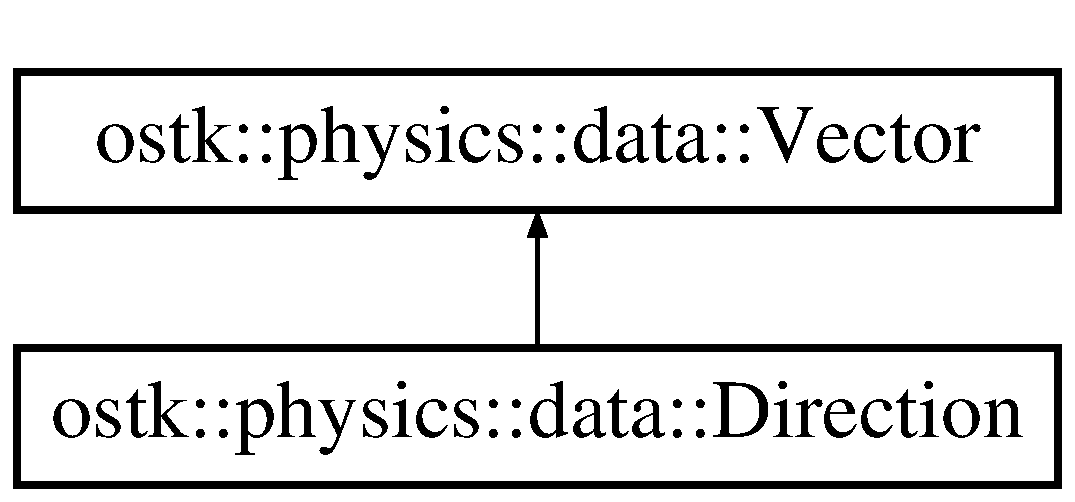
\includegraphics[height=2.000000cm]{classostk_1_1physics_1_1data_1_1_vector}
\end{center}
\end{figure}
\subsection*{Public Member Functions}
\begin{DoxyCompactItemize}
\item 
\hyperlink{classostk_1_1physics_1_1data_1_1_vector_a513244719d0a6b4a37537ed5c9bb2c27}{Vector} (const Vector3d \&a\+Value, const \hyperlink{classostk_1_1physics_1_1_unit}{Unit} \&a\+Unit, const Shared$<$ const \hyperlink{classostk_1_1physics_1_1coord_1_1_frame}{Frame} $>$ \&a\+Frame\+S\+Ptr)
\item 
bool \hyperlink{classostk_1_1physics_1_1data_1_1_vector_a4be0fe51a56b19eb4c7252436944b382}{operator==} (const \hyperlink{classostk_1_1physics_1_1data_1_1_vector}{Vector} \&a\+Vector) const
\item 
bool \hyperlink{classostk_1_1physics_1_1data_1_1_vector_a732642a94770c1486537368c44a0d434}{operator!=} (const \hyperlink{classostk_1_1physics_1_1data_1_1_vector}{Vector} \&a\+Vector) const
\item 
bool \hyperlink{classostk_1_1physics_1_1data_1_1_vector_aa5fee0fe657ba4b33e835ed4df37d0e1}{is\+Defined} () const
\item 
Vector3d \hyperlink{classostk_1_1physics_1_1data_1_1_vector_a33bd2c79920db43a8335918da8d5e79b}{get\+Value} () const
\item 
\hyperlink{classostk_1_1physics_1_1_unit}{Unit} \hyperlink{classostk_1_1physics_1_1data_1_1_vector_a467f0ab9ff5d9e83c6e3ce64ebfb8c95}{get\+Unit} () const
\item 
Shared$<$ const \hyperlink{classostk_1_1physics_1_1coord_1_1_frame}{Frame} $>$ \hyperlink{classostk_1_1physics_1_1data_1_1_vector_a39b99207e2617954be6629916d327fb6}{get\+Frame} () const
\item 
\hyperlink{classostk_1_1physics_1_1data_1_1_vector}{Vector} \hyperlink{classostk_1_1physics_1_1data_1_1_vector_a0ea065eeb3ccb829951c81c206eefd76}{in\+Unit} (const \hyperlink{classostk_1_1physics_1_1_unit}{Unit} \&a\+Unit) const
\item 
\hyperlink{classostk_1_1physics_1_1data_1_1_vector}{Vector} \hyperlink{classostk_1_1physics_1_1data_1_1_vector_af297f2ff4ae6d6e52aba683c6c78ab94}{in\+Frame} (const Shared$<$ const \hyperlink{classostk_1_1physics_1_1coord_1_1_frame}{Frame} $>$ \&a\+Frame\+S\+Ptr, const \hyperlink{classostk_1_1physics_1_1time_1_1_instant}{Instant} \&an\+Instant) const
\item 
String \hyperlink{classostk_1_1physics_1_1data_1_1_vector_aa1350ef1a2124c98a47900a0d81b5506}{to\+String} (const Integer \&a\+Precision=Integer\+::\+Undefined()) const
\end{DoxyCompactItemize}
\subsection*{Static Public Member Functions}
\begin{DoxyCompactItemize}
\item 
static \hyperlink{classostk_1_1physics_1_1data_1_1_vector}{Vector} \hyperlink{classostk_1_1physics_1_1data_1_1_vector_afb204c378708fdd162844a348da32db7}{Undefined} ()
\end{DoxyCompactItemize}
\subsection*{Friends}
\begin{DoxyCompactItemize}
\item 
std\+::ostream \& \hyperlink{classostk_1_1physics_1_1data_1_1_vector_a2f1253dbad20965d2209456421eabf71}{operator$<$$<$} (std\+::ostream \&an\+Output\+Stream, const \hyperlink{classostk_1_1physics_1_1data_1_1_vector}{Vector} \&a\+Vector)
\end{DoxyCompactItemize}


\subsection{Detailed Description}
\hyperlink{classostk_1_1physics_1_1data_1_1_vector}{Vector} quantity. 

\subsection{Constructor \& Destructor Documentation}
\mbox{\Hypertarget{classostk_1_1physics_1_1data_1_1_vector_a513244719d0a6b4a37537ed5c9bb2c27}\label{classostk_1_1physics_1_1data_1_1_vector_a513244719d0a6b4a37537ed5c9bb2c27}} 
\index{ostk\+::physics\+::data\+::\+Vector@{ostk\+::physics\+::data\+::\+Vector}!Vector@{Vector}}
\index{Vector@{Vector}!ostk\+::physics\+::data\+::\+Vector@{ostk\+::physics\+::data\+::\+Vector}}
\subsubsection{\texorpdfstring{Vector()}{Vector()}}
{\footnotesize\ttfamily ostk\+::physics\+::data\+::\+Vector\+::\+Vector (\begin{DoxyParamCaption}\item[{const Vector3d \&}]{a\+Value,  }\item[{const \hyperlink{classostk_1_1physics_1_1_unit}{Unit} \&}]{a\+Unit,  }\item[{const Shared$<$ const \hyperlink{classostk_1_1physics_1_1coord_1_1_frame}{Frame} $>$ \&}]{a\+Frame\+S\+Ptr }\end{DoxyParamCaption})}



\subsection{Member Function Documentation}
\mbox{\Hypertarget{classostk_1_1physics_1_1data_1_1_vector_a39b99207e2617954be6629916d327fb6}\label{classostk_1_1physics_1_1data_1_1_vector_a39b99207e2617954be6629916d327fb6}} 
\index{ostk\+::physics\+::data\+::\+Vector@{ostk\+::physics\+::data\+::\+Vector}!get\+Frame@{get\+Frame}}
\index{get\+Frame@{get\+Frame}!ostk\+::physics\+::data\+::\+Vector@{ostk\+::physics\+::data\+::\+Vector}}
\subsubsection{\texorpdfstring{get\+Frame()}{getFrame()}}
{\footnotesize\ttfamily Shared$<$ const \hyperlink{classostk_1_1physics_1_1coord_1_1_frame}{Frame} $>$ ostk\+::physics\+::data\+::\+Vector\+::get\+Frame (\begin{DoxyParamCaption}{ }\end{DoxyParamCaption}) const}

\mbox{\Hypertarget{classostk_1_1physics_1_1data_1_1_vector_a467f0ab9ff5d9e83c6e3ce64ebfb8c95}\label{classostk_1_1physics_1_1data_1_1_vector_a467f0ab9ff5d9e83c6e3ce64ebfb8c95}} 
\index{ostk\+::physics\+::data\+::\+Vector@{ostk\+::physics\+::data\+::\+Vector}!get\+Unit@{get\+Unit}}
\index{get\+Unit@{get\+Unit}!ostk\+::physics\+::data\+::\+Vector@{ostk\+::physics\+::data\+::\+Vector}}
\subsubsection{\texorpdfstring{get\+Unit()}{getUnit()}}
{\footnotesize\ttfamily \hyperlink{classostk_1_1physics_1_1_unit}{Unit} ostk\+::physics\+::data\+::\+Vector\+::get\+Unit (\begin{DoxyParamCaption}{ }\end{DoxyParamCaption}) const}

\mbox{\Hypertarget{classostk_1_1physics_1_1data_1_1_vector_a33bd2c79920db43a8335918da8d5e79b}\label{classostk_1_1physics_1_1data_1_1_vector_a33bd2c79920db43a8335918da8d5e79b}} 
\index{ostk\+::physics\+::data\+::\+Vector@{ostk\+::physics\+::data\+::\+Vector}!get\+Value@{get\+Value}}
\index{get\+Value@{get\+Value}!ostk\+::physics\+::data\+::\+Vector@{ostk\+::physics\+::data\+::\+Vector}}
\subsubsection{\texorpdfstring{get\+Value()}{getValue()}}
{\footnotesize\ttfamily Vector3d ostk\+::physics\+::data\+::\+Vector\+::get\+Value (\begin{DoxyParamCaption}{ }\end{DoxyParamCaption}) const}

\mbox{\Hypertarget{classostk_1_1physics_1_1data_1_1_vector_af297f2ff4ae6d6e52aba683c6c78ab94}\label{classostk_1_1physics_1_1data_1_1_vector_af297f2ff4ae6d6e52aba683c6c78ab94}} 
\index{ostk\+::physics\+::data\+::\+Vector@{ostk\+::physics\+::data\+::\+Vector}!in\+Frame@{in\+Frame}}
\index{in\+Frame@{in\+Frame}!ostk\+::physics\+::data\+::\+Vector@{ostk\+::physics\+::data\+::\+Vector}}
\subsubsection{\texorpdfstring{in\+Frame()}{inFrame()}}
{\footnotesize\ttfamily \hyperlink{classostk_1_1physics_1_1data_1_1_vector}{Vector} ostk\+::physics\+::data\+::\+Vector\+::in\+Frame (\begin{DoxyParamCaption}\item[{const Shared$<$ const \hyperlink{classostk_1_1physics_1_1coord_1_1_frame}{Frame} $>$ \&}]{a\+Frame\+S\+Ptr,  }\item[{const \hyperlink{classostk_1_1physics_1_1time_1_1_instant}{Instant} \&}]{an\+Instant }\end{DoxyParamCaption}) const}

\mbox{\Hypertarget{classostk_1_1physics_1_1data_1_1_vector_a0ea065eeb3ccb829951c81c206eefd76}\label{classostk_1_1physics_1_1data_1_1_vector_a0ea065eeb3ccb829951c81c206eefd76}} 
\index{ostk\+::physics\+::data\+::\+Vector@{ostk\+::physics\+::data\+::\+Vector}!in\+Unit@{in\+Unit}}
\index{in\+Unit@{in\+Unit}!ostk\+::physics\+::data\+::\+Vector@{ostk\+::physics\+::data\+::\+Vector}}
\subsubsection{\texorpdfstring{in\+Unit()}{inUnit()}}
{\footnotesize\ttfamily \hyperlink{classostk_1_1physics_1_1data_1_1_vector}{Vector} ostk\+::physics\+::data\+::\+Vector\+::in\+Unit (\begin{DoxyParamCaption}\item[{const \hyperlink{classostk_1_1physics_1_1_unit}{Unit} \&}]{a\+Unit }\end{DoxyParamCaption}) const}

\mbox{\Hypertarget{classostk_1_1physics_1_1data_1_1_vector_aa5fee0fe657ba4b33e835ed4df37d0e1}\label{classostk_1_1physics_1_1data_1_1_vector_aa5fee0fe657ba4b33e835ed4df37d0e1}} 
\index{ostk\+::physics\+::data\+::\+Vector@{ostk\+::physics\+::data\+::\+Vector}!is\+Defined@{is\+Defined}}
\index{is\+Defined@{is\+Defined}!ostk\+::physics\+::data\+::\+Vector@{ostk\+::physics\+::data\+::\+Vector}}
\subsubsection{\texorpdfstring{is\+Defined()}{isDefined()}}
{\footnotesize\ttfamily bool ostk\+::physics\+::data\+::\+Vector\+::is\+Defined (\begin{DoxyParamCaption}{ }\end{DoxyParamCaption}) const}

\mbox{\Hypertarget{classostk_1_1physics_1_1data_1_1_vector_a732642a94770c1486537368c44a0d434}\label{classostk_1_1physics_1_1data_1_1_vector_a732642a94770c1486537368c44a0d434}} 
\index{ostk\+::physics\+::data\+::\+Vector@{ostk\+::physics\+::data\+::\+Vector}!operator"!=@{operator"!=}}
\index{operator"!=@{operator"!=}!ostk\+::physics\+::data\+::\+Vector@{ostk\+::physics\+::data\+::\+Vector}}
\subsubsection{\texorpdfstring{operator"!=()}{operator!=()}}
{\footnotesize\ttfamily bool ostk\+::physics\+::data\+::\+Vector\+::operator!= (\begin{DoxyParamCaption}\item[{const \hyperlink{classostk_1_1physics_1_1data_1_1_vector}{Vector} \&}]{a\+Vector }\end{DoxyParamCaption}) const}

\mbox{\Hypertarget{classostk_1_1physics_1_1data_1_1_vector_a4be0fe51a56b19eb4c7252436944b382}\label{classostk_1_1physics_1_1data_1_1_vector_a4be0fe51a56b19eb4c7252436944b382}} 
\index{ostk\+::physics\+::data\+::\+Vector@{ostk\+::physics\+::data\+::\+Vector}!operator==@{operator==}}
\index{operator==@{operator==}!ostk\+::physics\+::data\+::\+Vector@{ostk\+::physics\+::data\+::\+Vector}}
\subsubsection{\texorpdfstring{operator==()}{operator==()}}
{\footnotesize\ttfamily bool ostk\+::physics\+::data\+::\+Vector\+::operator== (\begin{DoxyParamCaption}\item[{const \hyperlink{classostk_1_1physics_1_1data_1_1_vector}{Vector} \&}]{a\+Vector }\end{DoxyParamCaption}) const}

\mbox{\Hypertarget{classostk_1_1physics_1_1data_1_1_vector_aa1350ef1a2124c98a47900a0d81b5506}\label{classostk_1_1physics_1_1data_1_1_vector_aa1350ef1a2124c98a47900a0d81b5506}} 
\index{ostk\+::physics\+::data\+::\+Vector@{ostk\+::physics\+::data\+::\+Vector}!to\+String@{to\+String}}
\index{to\+String@{to\+String}!ostk\+::physics\+::data\+::\+Vector@{ostk\+::physics\+::data\+::\+Vector}}
\subsubsection{\texorpdfstring{to\+String()}{toString()}}
{\footnotesize\ttfamily String ostk\+::physics\+::data\+::\+Vector\+::to\+String (\begin{DoxyParamCaption}\item[{const Integer \&}]{a\+Precision = {\ttfamily Integer\+:\+:Undefined()} }\end{DoxyParamCaption}) const}

\mbox{\Hypertarget{classostk_1_1physics_1_1data_1_1_vector_afb204c378708fdd162844a348da32db7}\label{classostk_1_1physics_1_1data_1_1_vector_afb204c378708fdd162844a348da32db7}} 
\index{ostk\+::physics\+::data\+::\+Vector@{ostk\+::physics\+::data\+::\+Vector}!Undefined@{Undefined}}
\index{Undefined@{Undefined}!ostk\+::physics\+::data\+::\+Vector@{ostk\+::physics\+::data\+::\+Vector}}
\subsubsection{\texorpdfstring{Undefined()}{Undefined()}}
{\footnotesize\ttfamily \hyperlink{classostk_1_1physics_1_1data_1_1_vector}{Vector} ostk\+::physics\+::data\+::\+Vector\+::\+Undefined (\begin{DoxyParamCaption}{ }\end{DoxyParamCaption})\hspace{0.3cm}{\ttfamily [static]}}



\subsection{Friends And Related Function Documentation}
\mbox{\Hypertarget{classostk_1_1physics_1_1data_1_1_vector_a2f1253dbad20965d2209456421eabf71}\label{classostk_1_1physics_1_1data_1_1_vector_a2f1253dbad20965d2209456421eabf71}} 
\index{ostk\+::physics\+::data\+::\+Vector@{ostk\+::physics\+::data\+::\+Vector}!operator$<$$<$@{operator$<$$<$}}
\index{operator$<$$<$@{operator$<$$<$}!ostk\+::physics\+::data\+::\+Vector@{ostk\+::physics\+::data\+::\+Vector}}
\subsubsection{\texorpdfstring{operator$<$$<$}{operator<<}}
{\footnotesize\ttfamily std\+::ostream\& operator$<$$<$ (\begin{DoxyParamCaption}\item[{std\+::ostream \&}]{an\+Output\+Stream,  }\item[{const \hyperlink{classostk_1_1physics_1_1data_1_1_vector}{Vector} \&}]{a\+Vector }\end{DoxyParamCaption})\hspace{0.3cm}{\ttfamily [friend]}}



The documentation for this class was generated from the following files\+:\begin{DoxyCompactItemize}
\item 
include/\+Open\+Space\+Toolkit/\+Physics/\+Data/\hyperlink{_vector_8hpp}{Vector.\+hpp}\item 
src/\+Open\+Space\+Toolkit/\+Physics/\+Data/\hyperlink{_vector_8cpp}{Vector.\+cpp}\end{DoxyCompactItemize}

\hypertarget{classostk_1_1physics_1_1coord_1_1_velocity}{}\section{ostk\+:\+:physics\+:\+:coord\+:\+:Velocity Class Reference}
\label{classostk_1_1physics_1_1coord_1_1_velocity}\index{ostk\+::physics\+::coord\+::\+Velocity@{ostk\+::physics\+::coord\+::\+Velocity}}


\hyperlink{classostk_1_1physics_1_1coord_1_1_velocity}{Velocity}.  




{\ttfamily \#include $<$Velocity.\+hpp$>$}

\subsection*{Public Types}
\begin{DoxyCompactItemize}
\item 
enum \hyperlink{classostk_1_1physics_1_1coord_1_1_velocity_a01701e56094328a31d0211da5ac1ba28}{Unit} \{ \hyperlink{classostk_1_1physics_1_1coord_1_1_velocity_a01701e56094328a31d0211da5ac1ba28aec0fc0100c4fc1ce4eea230c3dc10360}{Unit\+::\+Undefined}, 
\hyperlink{classostk_1_1physics_1_1coord_1_1_velocity_a01701e56094328a31d0211da5ac1ba28a0af408165b5f88fcd7b687312b754ade}{Unit\+::\+Meter\+Per\+Second}
 \}
\end{DoxyCompactItemize}
\subsection*{Public Member Functions}
\begin{DoxyCompactItemize}
\item 
\hyperlink{classostk_1_1physics_1_1coord_1_1_velocity_a2e45f5a6e1025cd21a2f5fa61c6a940a}{Velocity} (const Vector3d \&a\+Coordinate\+Set, const \hyperlink{classostk_1_1physics_1_1coord_1_1_velocity_a01701e56094328a31d0211da5ac1ba28}{Velocity\+::\+Unit} \&a\+Unit, const Shared$<$ const \hyperlink{classostk_1_1physics_1_1coord_1_1_frame}{Frame} $>$ \&a\+Frame\+S\+Ptr)
\item 
bool \hyperlink{classostk_1_1physics_1_1coord_1_1_velocity_abadc0cc438b95d0820aa82603a0cd25b}{operator==} (const \hyperlink{classostk_1_1physics_1_1coord_1_1_velocity}{Velocity} \&a\+Velocity) const
\item 
bool \hyperlink{classostk_1_1physics_1_1coord_1_1_velocity_a83127c62ea6ce9497f57622a2ea3dbf0}{operator!=} (const \hyperlink{classostk_1_1physics_1_1coord_1_1_velocity}{Velocity} \&a\+Velocity) const
\item 
bool \hyperlink{classostk_1_1physics_1_1coord_1_1_velocity_a19318a3cef12b4248cd12e043ee41591}{is\+Defined} () const
\item 
const Vector3d \& \hyperlink{classostk_1_1physics_1_1coord_1_1_velocity_a2c567b0c5a5d2036e5ba8a043ddda598}{access\+Coordinates} () const
\item 
Shared$<$ const \hyperlink{classostk_1_1physics_1_1coord_1_1_frame}{Frame} $>$ \hyperlink{classostk_1_1physics_1_1coord_1_1_velocity_aa2f7454c6f34503989d6adf2e5d581f6}{access\+Frame} () const
\item 
Vector3d \hyperlink{classostk_1_1physics_1_1coord_1_1_velocity_a50636bdf695b2765ea94a5b76258ebc3}{get\+Coordinates} () const
\item 
\hyperlink{classostk_1_1physics_1_1coord_1_1_velocity_a01701e56094328a31d0211da5ac1ba28}{Velocity\+::\+Unit} \hyperlink{classostk_1_1physics_1_1coord_1_1_velocity_ae512730ddb567de93fe9f77e116557a0}{get\+Unit} () const
\item 
\hyperlink{classostk_1_1physics_1_1coord_1_1_velocity}{Velocity} \hyperlink{classostk_1_1physics_1_1coord_1_1_velocity_abafe2a4415f6bee5cdb0abd2c0b7d3dd}{in\+Unit} (const \hyperlink{classostk_1_1physics_1_1coord_1_1_velocity_a01701e56094328a31d0211da5ac1ba28}{Velocity\+::\+Unit} \&a\+Unit) const
\item 
\hyperlink{classostk_1_1physics_1_1coord_1_1_velocity}{Velocity} \hyperlink{classostk_1_1physics_1_1coord_1_1_velocity_aedf31d29406d85a2d302e7a5d51af4f3}{in\+Frame} (const \hyperlink{classostk_1_1physics_1_1coord_1_1_position}{Position} \&a\+Position, const Shared$<$ const \hyperlink{classostk_1_1physics_1_1coord_1_1_frame}{Frame} $>$ \&a\+Frame\+S\+Ptr, const \hyperlink{classostk_1_1physics_1_1time_1_1_instant}{Instant} \&an\+Instant) const
\item 
String \hyperlink{classostk_1_1physics_1_1coord_1_1_velocity_a130159d8ac35bd33440cb1890d65e8a5}{to\+String} (const Integer \&a\+Precision=Integer\+::\+Undefined()) const
\end{DoxyCompactItemize}
\subsection*{Static Public Member Functions}
\begin{DoxyCompactItemize}
\item 
static \hyperlink{classostk_1_1physics_1_1coord_1_1_velocity}{Velocity} \hyperlink{classostk_1_1physics_1_1coord_1_1_velocity_a3eb51fc62403ba59256b5b0a816a6392}{Undefined} ()
\item 
static \hyperlink{classostk_1_1physics_1_1coord_1_1_velocity}{Velocity} \hyperlink{classostk_1_1physics_1_1coord_1_1_velocity_a9c21dc239f2109c9698ac752b3d395b7}{Meters\+Per\+Second} (const Vector3d \&a\+Coordinate\+Set, const Shared$<$ const \hyperlink{classostk_1_1physics_1_1coord_1_1_frame}{Frame} $>$ \&a\+Frame\+S\+Ptr)
\item 
static String \hyperlink{classostk_1_1physics_1_1coord_1_1_velocity_a9a016d320278b1de234fa5dc2c96370d}{String\+From\+Unit} (const \hyperlink{classostk_1_1physics_1_1coord_1_1_velocity_a01701e56094328a31d0211da5ac1ba28}{Velocity\+::\+Unit} \&a\+Unit)
\end{DoxyCompactItemize}
\subsection*{Friends}
\begin{DoxyCompactItemize}
\item 
std\+::ostream \& \hyperlink{classostk_1_1physics_1_1coord_1_1_velocity_ab3987a176df736aa7fa50aa763ed068b}{operator$<$$<$} (std\+::ostream \&an\+Output\+Stream, const \hyperlink{classostk_1_1physics_1_1coord_1_1_velocity}{Velocity} \&a\+Velocity)
\end{DoxyCompactItemize}


\subsection{Detailed Description}
\hyperlink{classostk_1_1physics_1_1coord_1_1_velocity}{Velocity}. 

\subsection{Member Enumeration Documentation}
\mbox{\Hypertarget{classostk_1_1physics_1_1coord_1_1_velocity_a01701e56094328a31d0211da5ac1ba28}\label{classostk_1_1physics_1_1coord_1_1_velocity_a01701e56094328a31d0211da5ac1ba28}} 
\index{ostk\+::physics\+::coord\+::\+Velocity@{ostk\+::physics\+::coord\+::\+Velocity}!Unit@{Unit}}
\index{Unit@{Unit}!ostk\+::physics\+::coord\+::\+Velocity@{ostk\+::physics\+::coord\+::\+Velocity}}
\subsubsection{\texorpdfstring{Unit}{Unit}}
{\footnotesize\ttfamily enum \hyperlink{classostk_1_1physics_1_1coord_1_1_velocity_a01701e56094328a31d0211da5ac1ba28}{ostk\+::physics\+::coord\+::\+Velocity\+::\+Unit}\hspace{0.3cm}{\ttfamily [strong]}}

\begin{DoxyEnumFields}{Enumerator}
\raisebox{\heightof{T}}[0pt][0pt]{\index{Undefined@{Undefined}!ostk\+::physics\+::coord\+::\+Velocity@{ostk\+::physics\+::coord\+::\+Velocity}}\index{ostk\+::physics\+::coord\+::\+Velocity@{ostk\+::physics\+::coord\+::\+Velocity}!Undefined@{Undefined}}}\mbox{\Hypertarget{classostk_1_1physics_1_1coord_1_1_velocity_a01701e56094328a31d0211da5ac1ba28aec0fc0100c4fc1ce4eea230c3dc10360}\label{classostk_1_1physics_1_1coord_1_1_velocity_a01701e56094328a31d0211da5ac1ba28aec0fc0100c4fc1ce4eea230c3dc10360}} 
Undefined&\\
\hline

\raisebox{\heightof{T}}[0pt][0pt]{\index{Meter\+Per\+Second@{Meter\+Per\+Second}!ostk\+::physics\+::coord\+::\+Velocity@{ostk\+::physics\+::coord\+::\+Velocity}}\index{ostk\+::physics\+::coord\+::\+Velocity@{ostk\+::physics\+::coord\+::\+Velocity}!Meter\+Per\+Second@{Meter\+Per\+Second}}}\mbox{\Hypertarget{classostk_1_1physics_1_1coord_1_1_velocity_a01701e56094328a31d0211da5ac1ba28a0af408165b5f88fcd7b687312b754ade}\label{classostk_1_1physics_1_1coord_1_1_velocity_a01701e56094328a31d0211da5ac1ba28a0af408165b5f88fcd7b687312b754ade}} 
Meter\+Per\+Second&\\
\hline

\end{DoxyEnumFields}


\subsection{Constructor \& Destructor Documentation}
\mbox{\Hypertarget{classostk_1_1physics_1_1coord_1_1_velocity_a2e45f5a6e1025cd21a2f5fa61c6a940a}\label{classostk_1_1physics_1_1coord_1_1_velocity_a2e45f5a6e1025cd21a2f5fa61c6a940a}} 
\index{ostk\+::physics\+::coord\+::\+Velocity@{ostk\+::physics\+::coord\+::\+Velocity}!Velocity@{Velocity}}
\index{Velocity@{Velocity}!ostk\+::physics\+::coord\+::\+Velocity@{ostk\+::physics\+::coord\+::\+Velocity}}
\subsubsection{\texorpdfstring{Velocity()}{Velocity()}}
{\footnotesize\ttfamily ostk\+::physics\+::coord\+::\+Velocity\+::\+Velocity (\begin{DoxyParamCaption}\item[{const Vector3d \&}]{a\+Coordinate\+Set,  }\item[{const \hyperlink{classostk_1_1physics_1_1coord_1_1_velocity_a01701e56094328a31d0211da5ac1ba28}{Velocity\+::\+Unit} \&}]{a\+Unit,  }\item[{const Shared$<$ const \hyperlink{classostk_1_1physics_1_1coord_1_1_frame}{Frame} $>$ \&}]{a\+Frame\+S\+Ptr }\end{DoxyParamCaption})}



\subsection{Member Function Documentation}
\mbox{\Hypertarget{classostk_1_1physics_1_1coord_1_1_velocity_a2c567b0c5a5d2036e5ba8a043ddda598}\label{classostk_1_1physics_1_1coord_1_1_velocity_a2c567b0c5a5d2036e5ba8a043ddda598}} 
\index{ostk\+::physics\+::coord\+::\+Velocity@{ostk\+::physics\+::coord\+::\+Velocity}!access\+Coordinates@{access\+Coordinates}}
\index{access\+Coordinates@{access\+Coordinates}!ostk\+::physics\+::coord\+::\+Velocity@{ostk\+::physics\+::coord\+::\+Velocity}}
\subsubsection{\texorpdfstring{access\+Coordinates()}{accessCoordinates()}}
{\footnotesize\ttfamily const Vector3d \& ostk\+::physics\+::coord\+::\+Velocity\+::access\+Coordinates (\begin{DoxyParamCaption}{ }\end{DoxyParamCaption}) const}

\mbox{\Hypertarget{classostk_1_1physics_1_1coord_1_1_velocity_aa2f7454c6f34503989d6adf2e5d581f6}\label{classostk_1_1physics_1_1coord_1_1_velocity_aa2f7454c6f34503989d6adf2e5d581f6}} 
\index{ostk\+::physics\+::coord\+::\+Velocity@{ostk\+::physics\+::coord\+::\+Velocity}!access\+Frame@{access\+Frame}}
\index{access\+Frame@{access\+Frame}!ostk\+::physics\+::coord\+::\+Velocity@{ostk\+::physics\+::coord\+::\+Velocity}}
\subsubsection{\texorpdfstring{access\+Frame()}{accessFrame()}}
{\footnotesize\ttfamily Shared$<$ const \hyperlink{classostk_1_1physics_1_1coord_1_1_frame}{Frame} $>$ ostk\+::physics\+::coord\+::\+Velocity\+::access\+Frame (\begin{DoxyParamCaption}{ }\end{DoxyParamCaption}) const}

\mbox{\Hypertarget{classostk_1_1physics_1_1coord_1_1_velocity_a50636bdf695b2765ea94a5b76258ebc3}\label{classostk_1_1physics_1_1coord_1_1_velocity_a50636bdf695b2765ea94a5b76258ebc3}} 
\index{ostk\+::physics\+::coord\+::\+Velocity@{ostk\+::physics\+::coord\+::\+Velocity}!get\+Coordinates@{get\+Coordinates}}
\index{get\+Coordinates@{get\+Coordinates}!ostk\+::physics\+::coord\+::\+Velocity@{ostk\+::physics\+::coord\+::\+Velocity}}
\subsubsection{\texorpdfstring{get\+Coordinates()}{getCoordinates()}}
{\footnotesize\ttfamily Vector3d ostk\+::physics\+::coord\+::\+Velocity\+::get\+Coordinates (\begin{DoxyParamCaption}{ }\end{DoxyParamCaption}) const}

\mbox{\Hypertarget{classostk_1_1physics_1_1coord_1_1_velocity_ae512730ddb567de93fe9f77e116557a0}\label{classostk_1_1physics_1_1coord_1_1_velocity_ae512730ddb567de93fe9f77e116557a0}} 
\index{ostk\+::physics\+::coord\+::\+Velocity@{ostk\+::physics\+::coord\+::\+Velocity}!get\+Unit@{get\+Unit}}
\index{get\+Unit@{get\+Unit}!ostk\+::physics\+::coord\+::\+Velocity@{ostk\+::physics\+::coord\+::\+Velocity}}
\subsubsection{\texorpdfstring{get\+Unit()}{getUnit()}}
{\footnotesize\ttfamily \hyperlink{classostk_1_1physics_1_1coord_1_1_velocity_a01701e56094328a31d0211da5ac1ba28}{Velocity\+::\+Unit} ostk\+::physics\+::coord\+::\+Velocity\+::get\+Unit (\begin{DoxyParamCaption}{ }\end{DoxyParamCaption}) const}

\mbox{\Hypertarget{classostk_1_1physics_1_1coord_1_1_velocity_aedf31d29406d85a2d302e7a5d51af4f3}\label{classostk_1_1physics_1_1coord_1_1_velocity_aedf31d29406d85a2d302e7a5d51af4f3}} 
\index{ostk\+::physics\+::coord\+::\+Velocity@{ostk\+::physics\+::coord\+::\+Velocity}!in\+Frame@{in\+Frame}}
\index{in\+Frame@{in\+Frame}!ostk\+::physics\+::coord\+::\+Velocity@{ostk\+::physics\+::coord\+::\+Velocity}}
\subsubsection{\texorpdfstring{in\+Frame()}{inFrame()}}
{\footnotesize\ttfamily \hyperlink{classostk_1_1physics_1_1coord_1_1_velocity}{Velocity} ostk\+::physics\+::coord\+::\+Velocity\+::in\+Frame (\begin{DoxyParamCaption}\item[{const \hyperlink{classostk_1_1physics_1_1coord_1_1_position}{Position} \&}]{a\+Position,  }\item[{const Shared$<$ const \hyperlink{classostk_1_1physics_1_1coord_1_1_frame}{Frame} $>$ \&}]{a\+Frame\+S\+Ptr,  }\item[{const \hyperlink{classostk_1_1physics_1_1time_1_1_instant}{Instant} \&}]{an\+Instant }\end{DoxyParamCaption}) const}

\mbox{\Hypertarget{classostk_1_1physics_1_1coord_1_1_velocity_abafe2a4415f6bee5cdb0abd2c0b7d3dd}\label{classostk_1_1physics_1_1coord_1_1_velocity_abafe2a4415f6bee5cdb0abd2c0b7d3dd}} 
\index{ostk\+::physics\+::coord\+::\+Velocity@{ostk\+::physics\+::coord\+::\+Velocity}!in\+Unit@{in\+Unit}}
\index{in\+Unit@{in\+Unit}!ostk\+::physics\+::coord\+::\+Velocity@{ostk\+::physics\+::coord\+::\+Velocity}}
\subsubsection{\texorpdfstring{in\+Unit()}{inUnit()}}
{\footnotesize\ttfamily \hyperlink{classostk_1_1physics_1_1coord_1_1_velocity}{Velocity} ostk\+::physics\+::coord\+::\+Velocity\+::in\+Unit (\begin{DoxyParamCaption}\item[{const \hyperlink{classostk_1_1physics_1_1coord_1_1_velocity_a01701e56094328a31d0211da5ac1ba28}{Velocity\+::\+Unit} \&}]{a\+Unit }\end{DoxyParamCaption}) const}

\mbox{\Hypertarget{classostk_1_1physics_1_1coord_1_1_velocity_a19318a3cef12b4248cd12e043ee41591}\label{classostk_1_1physics_1_1coord_1_1_velocity_a19318a3cef12b4248cd12e043ee41591}} 
\index{ostk\+::physics\+::coord\+::\+Velocity@{ostk\+::physics\+::coord\+::\+Velocity}!is\+Defined@{is\+Defined}}
\index{is\+Defined@{is\+Defined}!ostk\+::physics\+::coord\+::\+Velocity@{ostk\+::physics\+::coord\+::\+Velocity}}
\subsubsection{\texorpdfstring{is\+Defined()}{isDefined()}}
{\footnotesize\ttfamily bool ostk\+::physics\+::coord\+::\+Velocity\+::is\+Defined (\begin{DoxyParamCaption}{ }\end{DoxyParamCaption}) const}

\mbox{\Hypertarget{classostk_1_1physics_1_1coord_1_1_velocity_a9c21dc239f2109c9698ac752b3d395b7}\label{classostk_1_1physics_1_1coord_1_1_velocity_a9c21dc239f2109c9698ac752b3d395b7}} 
\index{ostk\+::physics\+::coord\+::\+Velocity@{ostk\+::physics\+::coord\+::\+Velocity}!Meters\+Per\+Second@{Meters\+Per\+Second}}
\index{Meters\+Per\+Second@{Meters\+Per\+Second}!ostk\+::physics\+::coord\+::\+Velocity@{ostk\+::physics\+::coord\+::\+Velocity}}
\subsubsection{\texorpdfstring{Meters\+Per\+Second()}{MetersPerSecond()}}
{\footnotesize\ttfamily \hyperlink{classostk_1_1physics_1_1coord_1_1_velocity}{Velocity} ostk\+::physics\+::coord\+::\+Velocity\+::\+Meters\+Per\+Second (\begin{DoxyParamCaption}\item[{const Vector3d \&}]{a\+Coordinate\+Set,  }\item[{const Shared$<$ const \hyperlink{classostk_1_1physics_1_1coord_1_1_frame}{Frame} $>$ \&}]{a\+Frame\+S\+Ptr }\end{DoxyParamCaption})\hspace{0.3cm}{\ttfamily [static]}}

\mbox{\Hypertarget{classostk_1_1physics_1_1coord_1_1_velocity_a83127c62ea6ce9497f57622a2ea3dbf0}\label{classostk_1_1physics_1_1coord_1_1_velocity_a83127c62ea6ce9497f57622a2ea3dbf0}} 
\index{ostk\+::physics\+::coord\+::\+Velocity@{ostk\+::physics\+::coord\+::\+Velocity}!operator"!=@{operator"!=}}
\index{operator"!=@{operator"!=}!ostk\+::physics\+::coord\+::\+Velocity@{ostk\+::physics\+::coord\+::\+Velocity}}
\subsubsection{\texorpdfstring{operator"!=()}{operator!=()}}
{\footnotesize\ttfamily bool ostk\+::physics\+::coord\+::\+Velocity\+::operator!= (\begin{DoxyParamCaption}\item[{const \hyperlink{classostk_1_1physics_1_1coord_1_1_velocity}{Velocity} \&}]{a\+Velocity }\end{DoxyParamCaption}) const}

\mbox{\Hypertarget{classostk_1_1physics_1_1coord_1_1_velocity_abadc0cc438b95d0820aa82603a0cd25b}\label{classostk_1_1physics_1_1coord_1_1_velocity_abadc0cc438b95d0820aa82603a0cd25b}} 
\index{ostk\+::physics\+::coord\+::\+Velocity@{ostk\+::physics\+::coord\+::\+Velocity}!operator==@{operator==}}
\index{operator==@{operator==}!ostk\+::physics\+::coord\+::\+Velocity@{ostk\+::physics\+::coord\+::\+Velocity}}
\subsubsection{\texorpdfstring{operator==()}{operator==()}}
{\footnotesize\ttfamily bool ostk\+::physics\+::coord\+::\+Velocity\+::operator== (\begin{DoxyParamCaption}\item[{const \hyperlink{classostk_1_1physics_1_1coord_1_1_velocity}{Velocity} \&}]{a\+Velocity }\end{DoxyParamCaption}) const}

\mbox{\Hypertarget{classostk_1_1physics_1_1coord_1_1_velocity_a9a016d320278b1de234fa5dc2c96370d}\label{classostk_1_1physics_1_1coord_1_1_velocity_a9a016d320278b1de234fa5dc2c96370d}} 
\index{ostk\+::physics\+::coord\+::\+Velocity@{ostk\+::physics\+::coord\+::\+Velocity}!String\+From\+Unit@{String\+From\+Unit}}
\index{String\+From\+Unit@{String\+From\+Unit}!ostk\+::physics\+::coord\+::\+Velocity@{ostk\+::physics\+::coord\+::\+Velocity}}
\subsubsection{\texorpdfstring{String\+From\+Unit()}{StringFromUnit()}}
{\footnotesize\ttfamily String ostk\+::physics\+::coord\+::\+Velocity\+::\+String\+From\+Unit (\begin{DoxyParamCaption}\item[{const \hyperlink{classostk_1_1physics_1_1coord_1_1_velocity_a01701e56094328a31d0211da5ac1ba28}{Velocity\+::\+Unit} \&}]{a\+Unit }\end{DoxyParamCaption})\hspace{0.3cm}{\ttfamily [static]}}

\mbox{\Hypertarget{classostk_1_1physics_1_1coord_1_1_velocity_a130159d8ac35bd33440cb1890d65e8a5}\label{classostk_1_1physics_1_1coord_1_1_velocity_a130159d8ac35bd33440cb1890d65e8a5}} 
\index{ostk\+::physics\+::coord\+::\+Velocity@{ostk\+::physics\+::coord\+::\+Velocity}!to\+String@{to\+String}}
\index{to\+String@{to\+String}!ostk\+::physics\+::coord\+::\+Velocity@{ostk\+::physics\+::coord\+::\+Velocity}}
\subsubsection{\texorpdfstring{to\+String()}{toString()}}
{\footnotesize\ttfamily String ostk\+::physics\+::coord\+::\+Velocity\+::to\+String (\begin{DoxyParamCaption}\item[{const Integer \&}]{a\+Precision = {\ttfamily Integer\+:\+:Undefined()} }\end{DoxyParamCaption}) const}

\mbox{\Hypertarget{classostk_1_1physics_1_1coord_1_1_velocity_a3eb51fc62403ba59256b5b0a816a6392}\label{classostk_1_1physics_1_1coord_1_1_velocity_a3eb51fc62403ba59256b5b0a816a6392}} 
\index{ostk\+::physics\+::coord\+::\+Velocity@{ostk\+::physics\+::coord\+::\+Velocity}!Undefined@{Undefined}}
\index{Undefined@{Undefined}!ostk\+::physics\+::coord\+::\+Velocity@{ostk\+::physics\+::coord\+::\+Velocity}}
\subsubsection{\texorpdfstring{Undefined()}{Undefined()}}
{\footnotesize\ttfamily \hyperlink{classostk_1_1physics_1_1coord_1_1_velocity}{Velocity} ostk\+::physics\+::coord\+::\+Velocity\+::\+Undefined (\begin{DoxyParamCaption}{ }\end{DoxyParamCaption})\hspace{0.3cm}{\ttfamily [static]}}



\subsection{Friends And Related Function Documentation}
\mbox{\Hypertarget{classostk_1_1physics_1_1coord_1_1_velocity_ab3987a176df736aa7fa50aa763ed068b}\label{classostk_1_1physics_1_1coord_1_1_velocity_ab3987a176df736aa7fa50aa763ed068b}} 
\index{ostk\+::physics\+::coord\+::\+Velocity@{ostk\+::physics\+::coord\+::\+Velocity}!operator$<$$<$@{operator$<$$<$}}
\index{operator$<$$<$@{operator$<$$<$}!ostk\+::physics\+::coord\+::\+Velocity@{ostk\+::physics\+::coord\+::\+Velocity}}
\subsubsection{\texorpdfstring{operator$<$$<$}{operator<<}}
{\footnotesize\ttfamily std\+::ostream\& operator$<$$<$ (\begin{DoxyParamCaption}\item[{std\+::ostream \&}]{an\+Output\+Stream,  }\item[{const \hyperlink{classostk_1_1physics_1_1coord_1_1_velocity}{Velocity} \&}]{a\+Velocity }\end{DoxyParamCaption})\hspace{0.3cm}{\ttfamily [friend]}}



The documentation for this class was generated from the following files\+:\begin{DoxyCompactItemize}
\item 
include/\+Open\+Space\+Toolkit/\+Physics/\+Coordinate/\hyperlink{_velocity_8hpp}{Velocity.\+hpp}\item 
src/\+Open\+Space\+Toolkit/\+Physics/\+Coordinate/\hyperlink{_velocity_8cpp}{Velocity.\+cpp}\end{DoxyCompactItemize}

\hypertarget{structostk_1_1physics_1_1env_1_1obj_1_1celest_1_1_earth_1_1_models_1_1_w_g_s84}{}\section{ostk\+:\+:physics\+:\+:env\+:\+:obj\+:\+:celest\+:\+:Earth\+:\+:Models\+:\+:W\+G\+S84 Struct Reference}
\label{structostk_1_1physics_1_1env_1_1obj_1_1celest_1_1_earth_1_1_models_1_1_w_g_s84}\index{ostk\+::physics\+::env\+::obj\+::celest\+::\+Earth\+::\+Models\+::\+W\+G\+S84@{ostk\+::physics\+::env\+::obj\+::celest\+::\+Earth\+::\+Models\+::\+W\+G\+S84}}


{\ttfamily \#include $<$Earth.\+hpp$>$}

\subsection*{Static Public Attributes}
\begin{DoxyCompactItemize}
\item 
static const \hyperlink{classostk_1_1physics_1_1units_1_1_derived}{Derived} \hyperlink{structostk_1_1physics_1_1env_1_1obj_1_1celest_1_1_earth_1_1_models_1_1_w_g_s84_ad9da871753c1f2bbe4f4d8ad2faf11ba}{Gravitational\+Parameter} = \{ 398600441800000.\+0, Gravitational\+Parameter\+S\+I\+Unit \}
\item 
static const \hyperlink{classostk_1_1physics_1_1units_1_1_length}{Length} \hyperlink{structostk_1_1physics_1_1env_1_1obj_1_1celest_1_1_earth_1_1_models_1_1_w_g_s84_a87a056bc54308532e8148c9d9addca5d}{Equatorial\+Radius} = \hyperlink{classostk_1_1physics_1_1units_1_1_length_ad227977ce00756791595796a0dd5ddd7}{Length\+::\+Meters}(6378137.\+0)
\item 
static const Real \hyperlink{structostk_1_1physics_1_1env_1_1obj_1_1celest_1_1_earth_1_1_models_1_1_w_g_s84_abf5d54a510bb9f9ba11cecdb60a16e17}{Flattening} = 1.\+0 / 298.\+257223563
\item 
static const Real \hyperlink{structostk_1_1physics_1_1env_1_1obj_1_1celest_1_1_earth_1_1_models_1_1_w_g_s84_ae42abb8da1cf5323b3b01e604a2743ce}{C20} = -\/4.\+841668500000e-\/04
\item 
static const Real \hyperlink{structostk_1_1physics_1_1env_1_1obj_1_1celest_1_1_earth_1_1_models_1_1_w_g_s84_ac4a0736f324dc3faf5f5b279e7daac45}{J2} = -\/\hyperlink{structostk_1_1physics_1_1env_1_1obj_1_1celest_1_1_earth_1_1_models_1_1_w_g_s84_ae42abb8da1cf5323b3b01e604a2743ce}{Earth\+::\+Models\+::\+W\+G\+S84\+::\+C20} $\ast$ std\+::sqrt(5.\+0)
\end{DoxyCompactItemize}


\subsection{Member Data Documentation}
\mbox{\Hypertarget{structostk_1_1physics_1_1env_1_1obj_1_1celest_1_1_earth_1_1_models_1_1_w_g_s84_ae42abb8da1cf5323b3b01e604a2743ce}\label{structostk_1_1physics_1_1env_1_1obj_1_1celest_1_1_earth_1_1_models_1_1_w_g_s84_ae42abb8da1cf5323b3b01e604a2743ce}} 
\index{ostk\+::physics\+::env\+::obj\+::celest\+::\+Earth\+::\+Models\+::\+W\+G\+S84@{ostk\+::physics\+::env\+::obj\+::celest\+::\+Earth\+::\+Models\+::\+W\+G\+S84}!C20@{C20}}
\index{C20@{C20}!ostk\+::physics\+::env\+::obj\+::celest\+::\+Earth\+::\+Models\+::\+W\+G\+S84@{ostk\+::physics\+::env\+::obj\+::celest\+::\+Earth\+::\+Models\+::\+W\+G\+S84}}
\subsubsection{\texorpdfstring{C20}{C20}}
{\footnotesize\ttfamily const Real ostk\+::physics\+::env\+::obj\+::celest\+::\+Earth\+::\+Models\+::\+W\+G\+S84\+::\+C20 = -\/4.\+841668500000e-\/04\hspace{0.3cm}{\ttfamily [static]}}

\mbox{\Hypertarget{structostk_1_1physics_1_1env_1_1obj_1_1celest_1_1_earth_1_1_models_1_1_w_g_s84_a87a056bc54308532e8148c9d9addca5d}\label{structostk_1_1physics_1_1env_1_1obj_1_1celest_1_1_earth_1_1_models_1_1_w_g_s84_a87a056bc54308532e8148c9d9addca5d}} 
\index{ostk\+::physics\+::env\+::obj\+::celest\+::\+Earth\+::\+Models\+::\+W\+G\+S84@{ostk\+::physics\+::env\+::obj\+::celest\+::\+Earth\+::\+Models\+::\+W\+G\+S84}!Equatorial\+Radius@{Equatorial\+Radius}}
\index{Equatorial\+Radius@{Equatorial\+Radius}!ostk\+::physics\+::env\+::obj\+::celest\+::\+Earth\+::\+Models\+::\+W\+G\+S84@{ostk\+::physics\+::env\+::obj\+::celest\+::\+Earth\+::\+Models\+::\+W\+G\+S84}}
\subsubsection{\texorpdfstring{Equatorial\+Radius}{EquatorialRadius}}
{\footnotesize\ttfamily const \hyperlink{classostk_1_1physics_1_1units_1_1_length}{Length} ostk\+::physics\+::env\+::obj\+::celest\+::\+Earth\+::\+Models\+::\+W\+G\+S84\+::\+Equatorial\+Radius = \hyperlink{classostk_1_1physics_1_1units_1_1_length_ad227977ce00756791595796a0dd5ddd7}{Length\+::\+Meters}(6378137.\+0)\hspace{0.3cm}{\ttfamily [static]}}

\mbox{\Hypertarget{structostk_1_1physics_1_1env_1_1obj_1_1celest_1_1_earth_1_1_models_1_1_w_g_s84_abf5d54a510bb9f9ba11cecdb60a16e17}\label{structostk_1_1physics_1_1env_1_1obj_1_1celest_1_1_earth_1_1_models_1_1_w_g_s84_abf5d54a510bb9f9ba11cecdb60a16e17}} 
\index{ostk\+::physics\+::env\+::obj\+::celest\+::\+Earth\+::\+Models\+::\+W\+G\+S84@{ostk\+::physics\+::env\+::obj\+::celest\+::\+Earth\+::\+Models\+::\+W\+G\+S84}!Flattening@{Flattening}}
\index{Flattening@{Flattening}!ostk\+::physics\+::env\+::obj\+::celest\+::\+Earth\+::\+Models\+::\+W\+G\+S84@{ostk\+::physics\+::env\+::obj\+::celest\+::\+Earth\+::\+Models\+::\+W\+G\+S84}}
\subsubsection{\texorpdfstring{Flattening}{Flattening}}
{\footnotesize\ttfamily const Real ostk\+::physics\+::env\+::obj\+::celest\+::\+Earth\+::\+Models\+::\+W\+G\+S84\+::\+Flattening = 1.\+0 / 298.\+257223563\hspace{0.3cm}{\ttfamily [static]}}

\mbox{\Hypertarget{structostk_1_1physics_1_1env_1_1obj_1_1celest_1_1_earth_1_1_models_1_1_w_g_s84_ad9da871753c1f2bbe4f4d8ad2faf11ba}\label{structostk_1_1physics_1_1env_1_1obj_1_1celest_1_1_earth_1_1_models_1_1_w_g_s84_ad9da871753c1f2bbe4f4d8ad2faf11ba}} 
\index{ostk\+::physics\+::env\+::obj\+::celest\+::\+Earth\+::\+Models\+::\+W\+G\+S84@{ostk\+::physics\+::env\+::obj\+::celest\+::\+Earth\+::\+Models\+::\+W\+G\+S84}!Gravitational\+Parameter@{Gravitational\+Parameter}}
\index{Gravitational\+Parameter@{Gravitational\+Parameter}!ostk\+::physics\+::env\+::obj\+::celest\+::\+Earth\+::\+Models\+::\+W\+G\+S84@{ostk\+::physics\+::env\+::obj\+::celest\+::\+Earth\+::\+Models\+::\+W\+G\+S84}}
\subsubsection{\texorpdfstring{Gravitational\+Parameter}{GravitationalParameter}}
{\footnotesize\ttfamily const \hyperlink{classostk_1_1physics_1_1units_1_1_derived}{Derived} ostk\+::physics\+::env\+::obj\+::celest\+::\+Earth\+::\+Models\+::\+W\+G\+S84\+::\+Gravitational\+Parameter = \{ 398600441800000.\+0, Gravitational\+Parameter\+S\+I\+Unit \}\hspace{0.3cm}{\ttfamily [static]}}

\mbox{\Hypertarget{structostk_1_1physics_1_1env_1_1obj_1_1celest_1_1_earth_1_1_models_1_1_w_g_s84_ac4a0736f324dc3faf5f5b279e7daac45}\label{structostk_1_1physics_1_1env_1_1obj_1_1celest_1_1_earth_1_1_models_1_1_w_g_s84_ac4a0736f324dc3faf5f5b279e7daac45}} 
\index{ostk\+::physics\+::env\+::obj\+::celest\+::\+Earth\+::\+Models\+::\+W\+G\+S84@{ostk\+::physics\+::env\+::obj\+::celest\+::\+Earth\+::\+Models\+::\+W\+G\+S84}!J2@{J2}}
\index{J2@{J2}!ostk\+::physics\+::env\+::obj\+::celest\+::\+Earth\+::\+Models\+::\+W\+G\+S84@{ostk\+::physics\+::env\+::obj\+::celest\+::\+Earth\+::\+Models\+::\+W\+G\+S84}}
\subsubsection{\texorpdfstring{J2}{J2}}
{\footnotesize\ttfamily const Real ostk\+::physics\+::env\+::obj\+::celest\+::\+Earth\+::\+Models\+::\+W\+G\+S84\+::\+J2 = -\/\hyperlink{structostk_1_1physics_1_1env_1_1obj_1_1celest_1_1_earth_1_1_models_1_1_w_g_s84_ae42abb8da1cf5323b3b01e604a2743ce}{Earth\+::\+Models\+::\+W\+G\+S84\+::\+C20} $\ast$ std\+::sqrt(5.\+0)\hspace{0.3cm}{\ttfamily [static]}}



The documentation for this struct was generated from the following files\+:\begin{DoxyCompactItemize}
\item 
include/\+Open\+Space\+Toolkit/\+Physics/\+Environment/\+Objects/\+Celestial\+Bodies/\hyperlink{_objects_2_celestial_bodies_2_earth_8hpp}{Earth.\+hpp}\item 
src/\+Open\+Space\+Toolkit/\+Physics/\+Environment/\+Objects/\+Celestial\+Bodies/\hyperlink{_objects_2_celestial_bodies_2_earth_8cpp}{Earth.\+cpp}\end{DoxyCompactItemize}

\hypertarget{structostk_1_1physics_1_1env_1_1obj_1_1celest_1_1_earth_1_1_models_1_1_w_g_s84___e_g_m96}{}\section{ostk\+:\+:physics\+:\+:env\+:\+:obj\+:\+:celest\+:\+:Earth\+:\+:Models\+:\+:W\+G\+S84\+\_\+\+E\+G\+M96 Struct Reference}
\label{structostk_1_1physics_1_1env_1_1obj_1_1celest_1_1_earth_1_1_models_1_1_w_g_s84___e_g_m96}\index{ostk\+::physics\+::env\+::obj\+::celest\+::\+Earth\+::\+Models\+::\+W\+G\+S84\+\_\+\+E\+G\+M96@{ostk\+::physics\+::env\+::obj\+::celest\+::\+Earth\+::\+Models\+::\+W\+G\+S84\+\_\+\+E\+G\+M96}}


{\ttfamily \#include $<$Earth.\+hpp$>$}

\subsection*{Static Public Attributes}
\begin{DoxyCompactItemize}
\item 
static const \hyperlink{classostk_1_1physics_1_1units_1_1_derived}{Derived} \hyperlink{structostk_1_1physics_1_1env_1_1obj_1_1celest_1_1_earth_1_1_models_1_1_w_g_s84___e_g_m96_aebd579460c76357fec71a575f0f11484}{Gravitational\+Parameter} = \{ 398600441800000.\+0, Gravitational\+Parameter\+S\+I\+Unit \}
\item 
static const \hyperlink{classostk_1_1physics_1_1units_1_1_length}{Length} \hyperlink{structostk_1_1physics_1_1env_1_1obj_1_1celest_1_1_earth_1_1_models_1_1_w_g_s84___e_g_m96_a85bd44d9f4f38605e2af7c199417d7a1}{Equatorial\+Radius} = \hyperlink{classostk_1_1physics_1_1units_1_1_length_ad227977ce00756791595796a0dd5ddd7}{Length\+::\+Meters}(6378137.\+0)
\item 
static const Real \hyperlink{structostk_1_1physics_1_1env_1_1obj_1_1celest_1_1_earth_1_1_models_1_1_w_g_s84___e_g_m96_ae37f4ee220d705159245256d91495d99}{Flattening} = 1.\+0 / 298.\+257223563
\item 
static const Real \hyperlink{structostk_1_1physics_1_1env_1_1obj_1_1celest_1_1_earth_1_1_models_1_1_w_g_s84___e_g_m96_a6a57d0c75b75b420a2ddd4429fd84e67}{C20} = -\/4.\+841653717360e-\/04
\item 
static const Real \hyperlink{structostk_1_1physics_1_1env_1_1obj_1_1celest_1_1_earth_1_1_models_1_1_w_g_s84___e_g_m96_a5c0a59466f80996ab50c5725637ebbec}{J2} = -\/\hyperlink{structostk_1_1physics_1_1env_1_1obj_1_1celest_1_1_earth_1_1_models_1_1_w_g_s84___e_g_m96_a6a57d0c75b75b420a2ddd4429fd84e67}{Earth\+::\+Models\+::\+W\+G\+S84\+\_\+\+E\+G\+M96\+::\+C20} $\ast$ std\+::sqrt(5.\+0)
\end{DoxyCompactItemize}


\subsection{Member Data Documentation}
\mbox{\Hypertarget{structostk_1_1physics_1_1env_1_1obj_1_1celest_1_1_earth_1_1_models_1_1_w_g_s84___e_g_m96_a6a57d0c75b75b420a2ddd4429fd84e67}\label{structostk_1_1physics_1_1env_1_1obj_1_1celest_1_1_earth_1_1_models_1_1_w_g_s84___e_g_m96_a6a57d0c75b75b420a2ddd4429fd84e67}} 
\index{ostk\+::physics\+::env\+::obj\+::celest\+::\+Earth\+::\+Models\+::\+W\+G\+S84\+\_\+\+E\+G\+M96@{ostk\+::physics\+::env\+::obj\+::celest\+::\+Earth\+::\+Models\+::\+W\+G\+S84\+\_\+\+E\+G\+M96}!C20@{C20}}
\index{C20@{C20}!ostk\+::physics\+::env\+::obj\+::celest\+::\+Earth\+::\+Models\+::\+W\+G\+S84\+\_\+\+E\+G\+M96@{ostk\+::physics\+::env\+::obj\+::celest\+::\+Earth\+::\+Models\+::\+W\+G\+S84\+\_\+\+E\+G\+M96}}
\subsubsection{\texorpdfstring{C20}{C20}}
{\footnotesize\ttfamily const Real ostk\+::physics\+::env\+::obj\+::celest\+::\+Earth\+::\+Models\+::\+W\+G\+S84\+\_\+\+E\+G\+M96\+::\+C20 = -\/4.\+841653717360e-\/04\hspace{0.3cm}{\ttfamily [static]}}

\mbox{\Hypertarget{structostk_1_1physics_1_1env_1_1obj_1_1celest_1_1_earth_1_1_models_1_1_w_g_s84___e_g_m96_a85bd44d9f4f38605e2af7c199417d7a1}\label{structostk_1_1physics_1_1env_1_1obj_1_1celest_1_1_earth_1_1_models_1_1_w_g_s84___e_g_m96_a85bd44d9f4f38605e2af7c199417d7a1}} 
\index{ostk\+::physics\+::env\+::obj\+::celest\+::\+Earth\+::\+Models\+::\+W\+G\+S84\+\_\+\+E\+G\+M96@{ostk\+::physics\+::env\+::obj\+::celest\+::\+Earth\+::\+Models\+::\+W\+G\+S84\+\_\+\+E\+G\+M96}!Equatorial\+Radius@{Equatorial\+Radius}}
\index{Equatorial\+Radius@{Equatorial\+Radius}!ostk\+::physics\+::env\+::obj\+::celest\+::\+Earth\+::\+Models\+::\+W\+G\+S84\+\_\+\+E\+G\+M96@{ostk\+::physics\+::env\+::obj\+::celest\+::\+Earth\+::\+Models\+::\+W\+G\+S84\+\_\+\+E\+G\+M96}}
\subsubsection{\texorpdfstring{Equatorial\+Radius}{EquatorialRadius}}
{\footnotesize\ttfamily const \hyperlink{classostk_1_1physics_1_1units_1_1_length}{Length} ostk\+::physics\+::env\+::obj\+::celest\+::\+Earth\+::\+Models\+::\+W\+G\+S84\+\_\+\+E\+G\+M96\+::\+Equatorial\+Radius = \hyperlink{classostk_1_1physics_1_1units_1_1_length_ad227977ce00756791595796a0dd5ddd7}{Length\+::\+Meters}(6378137.\+0)\hspace{0.3cm}{\ttfamily [static]}}

\mbox{\Hypertarget{structostk_1_1physics_1_1env_1_1obj_1_1celest_1_1_earth_1_1_models_1_1_w_g_s84___e_g_m96_ae37f4ee220d705159245256d91495d99}\label{structostk_1_1physics_1_1env_1_1obj_1_1celest_1_1_earth_1_1_models_1_1_w_g_s84___e_g_m96_ae37f4ee220d705159245256d91495d99}} 
\index{ostk\+::physics\+::env\+::obj\+::celest\+::\+Earth\+::\+Models\+::\+W\+G\+S84\+\_\+\+E\+G\+M96@{ostk\+::physics\+::env\+::obj\+::celest\+::\+Earth\+::\+Models\+::\+W\+G\+S84\+\_\+\+E\+G\+M96}!Flattening@{Flattening}}
\index{Flattening@{Flattening}!ostk\+::physics\+::env\+::obj\+::celest\+::\+Earth\+::\+Models\+::\+W\+G\+S84\+\_\+\+E\+G\+M96@{ostk\+::physics\+::env\+::obj\+::celest\+::\+Earth\+::\+Models\+::\+W\+G\+S84\+\_\+\+E\+G\+M96}}
\subsubsection{\texorpdfstring{Flattening}{Flattening}}
{\footnotesize\ttfamily const Real ostk\+::physics\+::env\+::obj\+::celest\+::\+Earth\+::\+Models\+::\+W\+G\+S84\+\_\+\+E\+G\+M96\+::\+Flattening = 1.\+0 / 298.\+257223563\hspace{0.3cm}{\ttfamily [static]}}

\mbox{\Hypertarget{structostk_1_1physics_1_1env_1_1obj_1_1celest_1_1_earth_1_1_models_1_1_w_g_s84___e_g_m96_aebd579460c76357fec71a575f0f11484}\label{structostk_1_1physics_1_1env_1_1obj_1_1celest_1_1_earth_1_1_models_1_1_w_g_s84___e_g_m96_aebd579460c76357fec71a575f0f11484}} 
\index{ostk\+::physics\+::env\+::obj\+::celest\+::\+Earth\+::\+Models\+::\+W\+G\+S84\+\_\+\+E\+G\+M96@{ostk\+::physics\+::env\+::obj\+::celest\+::\+Earth\+::\+Models\+::\+W\+G\+S84\+\_\+\+E\+G\+M96}!Gravitational\+Parameter@{Gravitational\+Parameter}}
\index{Gravitational\+Parameter@{Gravitational\+Parameter}!ostk\+::physics\+::env\+::obj\+::celest\+::\+Earth\+::\+Models\+::\+W\+G\+S84\+\_\+\+E\+G\+M96@{ostk\+::physics\+::env\+::obj\+::celest\+::\+Earth\+::\+Models\+::\+W\+G\+S84\+\_\+\+E\+G\+M96}}
\subsubsection{\texorpdfstring{Gravitational\+Parameter}{GravitationalParameter}}
{\footnotesize\ttfamily const \hyperlink{classostk_1_1physics_1_1units_1_1_derived}{Derived} ostk\+::physics\+::env\+::obj\+::celest\+::\+Earth\+::\+Models\+::\+W\+G\+S84\+\_\+\+E\+G\+M96\+::\+Gravitational\+Parameter = \{ 398600441800000.\+0, Gravitational\+Parameter\+S\+I\+Unit \}\hspace{0.3cm}{\ttfamily [static]}}

\mbox{\Hypertarget{structostk_1_1physics_1_1env_1_1obj_1_1celest_1_1_earth_1_1_models_1_1_w_g_s84___e_g_m96_a5c0a59466f80996ab50c5725637ebbec}\label{structostk_1_1physics_1_1env_1_1obj_1_1celest_1_1_earth_1_1_models_1_1_w_g_s84___e_g_m96_a5c0a59466f80996ab50c5725637ebbec}} 
\index{ostk\+::physics\+::env\+::obj\+::celest\+::\+Earth\+::\+Models\+::\+W\+G\+S84\+\_\+\+E\+G\+M96@{ostk\+::physics\+::env\+::obj\+::celest\+::\+Earth\+::\+Models\+::\+W\+G\+S84\+\_\+\+E\+G\+M96}!J2@{J2}}
\index{J2@{J2}!ostk\+::physics\+::env\+::obj\+::celest\+::\+Earth\+::\+Models\+::\+W\+G\+S84\+\_\+\+E\+G\+M96@{ostk\+::physics\+::env\+::obj\+::celest\+::\+Earth\+::\+Models\+::\+W\+G\+S84\+\_\+\+E\+G\+M96}}
\subsubsection{\texorpdfstring{J2}{J2}}
{\footnotesize\ttfamily const Real ostk\+::physics\+::env\+::obj\+::celest\+::\+Earth\+::\+Models\+::\+W\+G\+S84\+\_\+\+E\+G\+M96\+::\+J2 = -\/\hyperlink{structostk_1_1physics_1_1env_1_1obj_1_1celest_1_1_earth_1_1_models_1_1_w_g_s84___e_g_m96_a6a57d0c75b75b420a2ddd4429fd84e67}{Earth\+::\+Models\+::\+W\+G\+S84\+\_\+\+E\+G\+M96\+::\+C20} $\ast$ std\+::sqrt(5.\+0)\hspace{0.3cm}{\ttfamily [static]}}



The documentation for this struct was generated from the following files\+:\begin{DoxyCompactItemize}
\item 
include/\+Open\+Space\+Toolkit/\+Physics/\+Environment/\+Objects/\+Celestial\+Bodies/\hyperlink{_objects_2_celestial_bodies_2_earth_8hpp}{Earth.\+hpp}\item 
src/\+Open\+Space\+Toolkit/\+Physics/\+Environment/\+Objects/\+Celestial\+Bodies/\hyperlink{_objects_2_celestial_bodies_2_earth_8cpp}{Earth.\+cpp}\end{DoxyCompactItemize}

\chapter{File Documentation}
\input{_c_o_n_t_r_i_b_u_t_i_n_g_8md}
\input{_tutorial_8md}
\hypertarget{_axes_8hpp}{}\section{include/\+Open\+Space\+Toolkit/\+Physics/\+Coordinate/\+Axes.hpp File Reference}
\label{_axes_8hpp}\index{include/\+Open\+Space\+Toolkit/\+Physics/\+Coordinate/\+Axes.\+hpp@{include/\+Open\+Space\+Toolkit/\+Physics/\+Coordinate/\+Axes.\+hpp}}
{\ttfamily \#include $<$Open\+Space\+Toolkit/\+Physics/\+Time/\+Instant.\+hpp$>$}\newline
{\ttfamily \#include $<$Open\+Space\+Toolkit/\+Mathematics/\+Objects/\+Vector.\+hpp$>$}\newline
{\ttfamily \#include $<$Open\+Space\+Toolkit/\+Core/\+Types/\+Shared.\+hpp$>$}\newline
\subsection*{Classes}
\begin{DoxyCompactItemize}
\item 
class \hyperlink{classostk_1_1physics_1_1coord_1_1_axes}{ostk\+::physics\+::coord\+::\+Axes}
\begin{DoxyCompactList}\small\item\em \hyperlink{classostk_1_1physics_1_1coord_1_1_axes}{Axes}. \end{DoxyCompactList}\end{DoxyCompactItemize}
\subsection*{Namespaces}
\begin{DoxyCompactItemize}
\item 
 \hyperlink{namespaceostk}{ostk}
\item 
 \hyperlink{namespaceostk_1_1physics}{ostk\+::physics}
\item 
 \hyperlink{namespaceostk_1_1physics_1_1coord}{ostk\+::physics\+::coord}
\end{DoxyCompactItemize}


\subsection{Detailed Description}
Open Space Toolkit ▸ Physics

\begin{DoxyAuthor}{Author}
Lucas Brémond \href{mailto:lucas@loftorbital.com}{\tt lucas@loftorbital.\+com}  Apache License 2.\+0 
\end{DoxyAuthor}

\hypertarget{_frame_8hpp}{}\section{include/\+Open\+Space\+Toolkit/\+Physics/\+Coordinate/\+Frame.hpp File Reference}
\label{_frame_8hpp}\index{include/\+Open\+Space\+Toolkit/\+Physics/\+Coordinate/\+Frame.\+hpp@{include/\+Open\+Space\+Toolkit/\+Physics/\+Coordinate/\+Frame.\+hpp}}
{\ttfamily \#include $<$Open\+Space\+Toolkit/\+Physics/\+Coordinate/\+Frame/\+Provider.\+hpp$>$}\newline
{\ttfamily \#include $<$Open\+Space\+Toolkit/\+Physics/\+Coordinate/\+Transform.\+hpp$>$}\newline
{\ttfamily \#include $<$Open\+Space\+Toolkit/\+Physics/\+Coordinate/\+Axes.\+hpp$>$}\newline
{\ttfamily \#include $<$Open\+Space\+Toolkit/\+Physics/\+Coordinate/\+Velocity.\+hpp$>$}\newline
{\ttfamily \#include $<$Open\+Space\+Toolkit/\+Physics/\+Coordinate/\+Position.\+hpp$>$}\newline
{\ttfamily \#include $<$Open\+Space\+Toolkit/\+Mathematics/\+Objects/\+Vector.\+hpp$>$}\newline
{\ttfamily \#include $<$Open\+Space\+Toolkit/\+Core/\+Types/\+String.\+hpp$>$}\newline
{\ttfamily \#include $<$Open\+Space\+Toolkit/\+Core/\+Types/\+Real.\+hpp$>$}\newline
{\ttfamily \#include $<$Open\+Space\+Toolkit/\+Core/\+Types/\+Integer.\+hpp$>$}\newline
{\ttfamily \#include $<$Open\+Space\+Toolkit/\+Core/\+Types/\+Shared.\+hpp$>$}\newline
{\ttfamily \#include $<$memory$>$}\newline
\subsection*{Classes}
\begin{DoxyCompactItemize}
\item 
class \hyperlink{classostk_1_1physics_1_1coord_1_1_frame}{ostk\+::physics\+::coord\+::\+Frame}
\begin{DoxyCompactList}\small\item\em Reference frame. \end{DoxyCompactList}\end{DoxyCompactItemize}
\subsection*{Namespaces}
\begin{DoxyCompactItemize}
\item 
 \hyperlink{namespaceostk}{ostk}
\item 
 \hyperlink{namespaceostk_1_1physics}{ostk\+::physics}
\item 
 \hyperlink{namespaceostk_1_1physics_1_1coord}{ostk\+::physics\+::coord}
\end{DoxyCompactItemize}


\subsection{Detailed Description}
Open Space Toolkit ▸ Physics

\begin{DoxyAuthor}{Author}
Lucas Brémond \href{mailto:lucas@loftorbital.com}{\tt lucas@loftorbital.\+com}  Apache License 2.\+0 
\end{DoxyAuthor}

\hypertarget{_coordinate_2_frame_2_manager_8hpp}{}\section{include/\+Open\+Space\+Toolkit/\+Physics/\+Coordinate/\+Frame/\+Manager.hpp File Reference}
\label{_coordinate_2_frame_2_manager_8hpp}\index{include/\+Open\+Space\+Toolkit/\+Physics/\+Coordinate/\+Frame/\+Manager.\+hpp@{include/\+Open\+Space\+Toolkit/\+Physics/\+Coordinate/\+Frame/\+Manager.\+hpp}}
{\ttfamily \#include $<$Open\+Space\+Toolkit/\+Physics/\+Coordinate/\+Transform.\+hpp$>$}\newline
{\ttfamily \#include $<$Open\+Space\+Toolkit/\+Physics/\+Coordinate/\+Frame.\+hpp$>$}\newline
{\ttfamily \#include $<$Open\+Space\+Toolkit/\+Physics/\+Time/\+Instant.\+hpp$>$}\newline
{\ttfamily \#include $<$Open\+Space\+Toolkit/\+Core/\+Containers/\+Map.\+hpp$>$}\newline
{\ttfamily \#include $<$Open\+Space\+Toolkit/\+Core/\+Types/\+String.\+hpp$>$}\newline
{\ttfamily \#include $<$Open\+Space\+Toolkit/\+Core/\+Types/\+Shared.\+hpp$>$}\newline
{\ttfamily \#include $<$mutex$>$}\newline
\subsection*{Classes}
\begin{DoxyCompactItemize}
\item 
class \hyperlink{classostk_1_1physics_1_1coord_1_1frame_1_1_manager}{ostk\+::physics\+::coord\+::frame\+::\+Manager}
\begin{DoxyCompactList}\small\item\em Reference frame manager (thread-\/safe) \end{DoxyCompactList}\end{DoxyCompactItemize}
\subsection*{Namespaces}
\begin{DoxyCompactItemize}
\item 
 \hyperlink{namespaceostk}{ostk}
\item 
 \hyperlink{namespaceostk_1_1physics}{ostk\+::physics}
\item 
 \hyperlink{namespaceostk_1_1physics_1_1coord}{ostk\+::physics\+::coord}
\item 
 \hyperlink{namespaceostk_1_1physics_1_1coord_1_1frame}{ostk\+::physics\+::coord\+::frame}
\end{DoxyCompactItemize}


\subsection{Detailed Description}
Open Space Toolkit ▸ Physics

\begin{DoxyAuthor}{Author}
Lucas Brémond \href{mailto:lucas@loftorbital.com}{\tt lucas@loftorbital.\+com}  Apache License 2.\+0 
\end{DoxyAuthor}

\hypertarget{_coordinate_2_frame_2_providers_2_i_e_r_s_2_manager_8hpp}{}\section{include/\+Library/\+Physics/\+Coordinate/\+Frame/\+Providers/\+I\+E\+R\+S/\+Manager.hpp File Reference}
\label{_coordinate_2_frame_2_providers_2_i_e_r_s_2_manager_8hpp}\index{include/\+Library/\+Physics/\+Coordinate/\+Frame/\+Providers/\+I\+E\+R\+S/\+Manager.\+hpp@{include/\+Library/\+Physics/\+Coordinate/\+Frame/\+Providers/\+I\+E\+R\+S/\+Manager.\+hpp}}
{\ttfamily \#include $<$Library/\+Physics/\+Coordinate/\+Frame/\+Providers/\+I\+E\+R\+S/\+Finals2000\+A.\+hpp$>$}\newline
{\ttfamily \#include $<$Library/\+Physics/\+Coordinate/\+Frame/\+Providers/\+I\+E\+R\+S/\+Bulletin\+A.\+hpp$>$}\newline
{\ttfamily \#include $<$Library/\+Physics/\+Time/\+Duration.\+hpp$>$}\newline
{\ttfamily \#include $<$Library/\+Physics/\+Time/\+Instant.\+hpp$>$}\newline
{\ttfamily \#include $<$Library/\+Mathematics/\+Objects/\+Vector.\+hpp$>$}\newline
{\ttfamily \#include $<$Library/\+I\+O/\+U\+R\+L.\+hpp$>$}\newline
{\ttfamily \#include $<$Library/\+Core/\+File\+System/\+Directory.\+hpp$>$}\newline
{\ttfamily \#include $<$Library/\+Core/\+Containers/\+Array.\+hpp$>$}\newline
{\ttfamily \#include $<$Library/\+Core/\+Types/\+Real.\+hpp$>$}\newline
{\ttfamily \#include $<$Library/\+Core/\+Types/\+Index.\+hpp$>$}\newline
{\ttfamily \#include $<$mutex$>$}\newline
\subsection*{Classes}
\begin{DoxyCompactItemize}
\item 
class \hyperlink{classlibrary_1_1physics_1_1coord_1_1frame_1_1provider_1_1iers_1_1_manager}{library\+::physics\+::coord\+::frame\+::provider\+::iers\+::\+Manager}
\begin{DoxyCompactList}\small\item\em I\+E\+RS bulletins manager (thread-\/safe) \end{DoxyCompactList}\end{DoxyCompactItemize}
\subsection*{Namespaces}
\begin{DoxyCompactItemize}
\item 
 \hyperlink{namespacelibrary}{library}
\item 
 \hyperlink{namespacelibrary_1_1physics}{library\+::physics}
\item 
 \hyperlink{namespacelibrary_1_1physics_1_1coord}{library\+::physics\+::coord}
\item 
 \hyperlink{namespacelibrary_1_1physics_1_1coord_1_1frame}{library\+::physics\+::coord\+::frame}
\item 
 \hyperlink{namespacelibrary_1_1physics_1_1coord_1_1frame_1_1provider}{library\+::physics\+::coord\+::frame\+::provider}
\item 
 \hyperlink{namespacelibrary_1_1physics_1_1coord_1_1frame_1_1provider_1_1iers}{library\+::physics\+::coord\+::frame\+::provider\+::iers}
\end{DoxyCompactItemize}
\subsection*{Macros}
\begin{DoxyCompactItemize}
\item 
\#define \hyperlink{_coordinate_2_frame_2_providers_2_i_e_r_s_2_manager_8hpp_af7c5a25598c85f3abde15d0d62a427a2}{L\+I\+B\+R\+A\+R\+Y\+\_\+\+P\+H\+Y\+S\+I\+C\+S\+\_\+\+C\+O\+O\+R\+D\+I\+N\+A\+T\+E\+\_\+\+F\+R\+A\+M\+E\+\_\+\+P\+R\+O\+V\+I\+D\+E\+R\+S\+\_\+\+I\+E\+R\+S\+\_\+\+M\+A\+N\+A\+G\+E\+R\+\_\+\+M\+O\+DE}~Manager\+::\+Mode\+::\+Manual
\item 
\#define \hyperlink{_coordinate_2_frame_2_providers_2_i_e_r_s_2_manager_8hpp_a3d95d418448eaba4f6dd5efb56c3c617}{L\+I\+B\+R\+A\+R\+Y\+\_\+\+P\+H\+Y\+S\+I\+C\+S\+\_\+\+C\+O\+O\+R\+D\+I\+N\+A\+T\+E\+\_\+\+F\+R\+A\+M\+E\+\_\+\+P\+R\+O\+V\+I\+D\+E\+R\+S\+\_\+\+I\+E\+R\+S\+\_\+\+M\+A\+N\+A\+G\+E\+R\+\_\+\+L\+O\+C\+A\+L\+\_\+\+R\+E\+P\+O\+S\+I\+T\+O\+RY}~\char`\"{}./.library/physics/coordinate/frame/providers/iers\char`\"{}
\item 
\#define \hyperlink{_coordinate_2_frame_2_providers_2_i_e_r_s_2_manager_8hpp_abed35c38a6c8603b3f02d97f68614c4e}{L\+I\+B\+R\+A\+R\+Y\+\_\+\+P\+H\+Y\+S\+I\+C\+S\+\_\+\+C\+O\+O\+R\+D\+I\+N\+A\+T\+E\+\_\+\+F\+R\+A\+M\+E\+\_\+\+P\+R\+O\+V\+I\+D\+E\+R\+S\+\_\+\+I\+E\+R\+S\+\_\+\+M\+A\+N\+A\+G\+E\+R\+\_\+\+L\+O\+C\+A\+L\+\_\+\+R\+E\+P\+O\+S\+I\+T\+O\+R\+Y\+\_\+\+L\+O\+C\+K\+\_\+\+T\+I\+M\+E\+O\+UT}~60
\item 
\#define \hyperlink{_coordinate_2_frame_2_providers_2_i_e_r_s_2_manager_8hpp_aa075c6efff4d21e8de829cc40e35ffd3}{L\+I\+B\+R\+A\+R\+Y\+\_\+\+P\+H\+Y\+S\+I\+C\+S\+\_\+\+C\+O\+O\+R\+D\+I\+N\+A\+T\+E\+\_\+\+F\+R\+A\+M\+E\+\_\+\+P\+R\+O\+V\+I\+D\+E\+R\+S\+\_\+\+I\+E\+R\+S\+\_\+\+M\+A\+N\+A\+G\+E\+R\+\_\+\+R\+E\+M\+O\+T\+E\+\_\+\+U\+RL}~\char`\"{}ftp\+://cddis.\+gsfc.\+nasa.\+gov/pub/products/iers/\char`\"{}
\end{DoxyCompactItemize}


\subsection{Detailed Description}
Library ▸ Physics

\begin{DoxyAuthor}{Author}
Lucas Brémond \href{mailto:lucas@loftorbital.com}{\tt lucas@loftorbital.\+com}  Apache License 2.\+0 
\end{DoxyAuthor}


\subsection{Macro Definition Documentation}
\mbox{\Hypertarget{_coordinate_2_frame_2_providers_2_i_e_r_s_2_manager_8hpp_a3d95d418448eaba4f6dd5efb56c3c617}\label{_coordinate_2_frame_2_providers_2_i_e_r_s_2_manager_8hpp_a3d95d418448eaba4f6dd5efb56c3c617}} 
\index{Coordinate/\+Frame/\+Providers/\+I\+E\+R\+S/\+Manager.\+hpp@{Coordinate/\+Frame/\+Providers/\+I\+E\+R\+S/\+Manager.\+hpp}!L\+I\+B\+R\+A\+R\+Y\+\_\+\+P\+H\+Y\+S\+I\+C\+S\+\_\+\+C\+O\+O\+R\+D\+I\+N\+A\+T\+E\+\_\+\+F\+R\+A\+M\+E\+\_\+\+P\+R\+O\+V\+I\+D\+E\+R\+S\+\_\+\+I\+E\+R\+S\+\_\+\+M\+A\+N\+A\+G\+E\+R\+\_\+\+L\+O\+C\+A\+L\+\_\+\+R\+E\+P\+O\+S\+I\+T\+O\+RY@{L\+I\+B\+R\+A\+R\+Y\+\_\+\+P\+H\+Y\+S\+I\+C\+S\+\_\+\+C\+O\+O\+R\+D\+I\+N\+A\+T\+E\+\_\+\+F\+R\+A\+M\+E\+\_\+\+P\+R\+O\+V\+I\+D\+E\+R\+S\+\_\+\+I\+E\+R\+S\+\_\+\+M\+A\+N\+A\+G\+E\+R\+\_\+\+L\+O\+C\+A\+L\+\_\+\+R\+E\+P\+O\+S\+I\+T\+O\+RY}}
\index{L\+I\+B\+R\+A\+R\+Y\+\_\+\+P\+H\+Y\+S\+I\+C\+S\+\_\+\+C\+O\+O\+R\+D\+I\+N\+A\+T\+E\+\_\+\+F\+R\+A\+M\+E\+\_\+\+P\+R\+O\+V\+I\+D\+E\+R\+S\+\_\+\+I\+E\+R\+S\+\_\+\+M\+A\+N\+A\+G\+E\+R\+\_\+\+L\+O\+C\+A\+L\+\_\+\+R\+E\+P\+O\+S\+I\+T\+O\+RY@{L\+I\+B\+R\+A\+R\+Y\+\_\+\+P\+H\+Y\+S\+I\+C\+S\+\_\+\+C\+O\+O\+R\+D\+I\+N\+A\+T\+E\+\_\+\+F\+R\+A\+M\+E\+\_\+\+P\+R\+O\+V\+I\+D\+E\+R\+S\+\_\+\+I\+E\+R\+S\+\_\+\+M\+A\+N\+A\+G\+E\+R\+\_\+\+L\+O\+C\+A\+L\+\_\+\+R\+E\+P\+O\+S\+I\+T\+O\+RY}!Coordinate/\+Frame/\+Providers/\+I\+E\+R\+S/\+Manager.\+hpp@{Coordinate/\+Frame/\+Providers/\+I\+E\+R\+S/\+Manager.\+hpp}}
\subsubsection{\texorpdfstring{L\+I\+B\+R\+A\+R\+Y\+\_\+\+P\+H\+Y\+S\+I\+C\+S\+\_\+\+C\+O\+O\+R\+D\+I\+N\+A\+T\+E\+\_\+\+F\+R\+A\+M\+E\+\_\+\+P\+R\+O\+V\+I\+D\+E\+R\+S\+\_\+\+I\+E\+R\+S\+\_\+\+M\+A\+N\+A\+G\+E\+R\+\_\+\+L\+O\+C\+A\+L\+\_\+\+R\+E\+P\+O\+S\+I\+T\+O\+RY}{LIBRARY\_PHYSICS\_COORDINATE\_FRAME\_PROVIDERS\_IERS\_MANAGER\_LOCAL\_REPOSITORY}}
{\footnotesize\ttfamily \#define L\+I\+B\+R\+A\+R\+Y\+\_\+\+P\+H\+Y\+S\+I\+C\+S\+\_\+\+C\+O\+O\+R\+D\+I\+N\+A\+T\+E\+\_\+\+F\+R\+A\+M\+E\+\_\+\+P\+R\+O\+V\+I\+D\+E\+R\+S\+\_\+\+I\+E\+R\+S\+\_\+\+M\+A\+N\+A\+G\+E\+R\+\_\+\+L\+O\+C\+A\+L\+\_\+\+R\+E\+P\+O\+S\+I\+T\+O\+RY~\char`\"{}./.library/physics/coordinate/frame/providers/iers\char`\"{}}

\mbox{\Hypertarget{_coordinate_2_frame_2_providers_2_i_e_r_s_2_manager_8hpp_abed35c38a6c8603b3f02d97f68614c4e}\label{_coordinate_2_frame_2_providers_2_i_e_r_s_2_manager_8hpp_abed35c38a6c8603b3f02d97f68614c4e}} 
\index{Coordinate/\+Frame/\+Providers/\+I\+E\+R\+S/\+Manager.\+hpp@{Coordinate/\+Frame/\+Providers/\+I\+E\+R\+S/\+Manager.\+hpp}!L\+I\+B\+R\+A\+R\+Y\+\_\+\+P\+H\+Y\+S\+I\+C\+S\+\_\+\+C\+O\+O\+R\+D\+I\+N\+A\+T\+E\+\_\+\+F\+R\+A\+M\+E\+\_\+\+P\+R\+O\+V\+I\+D\+E\+R\+S\+\_\+\+I\+E\+R\+S\+\_\+\+M\+A\+N\+A\+G\+E\+R\+\_\+\+L\+O\+C\+A\+L\+\_\+\+R\+E\+P\+O\+S\+I\+T\+O\+R\+Y\+\_\+\+L\+O\+C\+K\+\_\+\+T\+I\+M\+E\+O\+UT@{L\+I\+B\+R\+A\+R\+Y\+\_\+\+P\+H\+Y\+S\+I\+C\+S\+\_\+\+C\+O\+O\+R\+D\+I\+N\+A\+T\+E\+\_\+\+F\+R\+A\+M\+E\+\_\+\+P\+R\+O\+V\+I\+D\+E\+R\+S\+\_\+\+I\+E\+R\+S\+\_\+\+M\+A\+N\+A\+G\+E\+R\+\_\+\+L\+O\+C\+A\+L\+\_\+\+R\+E\+P\+O\+S\+I\+T\+O\+R\+Y\+\_\+\+L\+O\+C\+K\+\_\+\+T\+I\+M\+E\+O\+UT}}
\index{L\+I\+B\+R\+A\+R\+Y\+\_\+\+P\+H\+Y\+S\+I\+C\+S\+\_\+\+C\+O\+O\+R\+D\+I\+N\+A\+T\+E\+\_\+\+F\+R\+A\+M\+E\+\_\+\+P\+R\+O\+V\+I\+D\+E\+R\+S\+\_\+\+I\+E\+R\+S\+\_\+\+M\+A\+N\+A\+G\+E\+R\+\_\+\+L\+O\+C\+A\+L\+\_\+\+R\+E\+P\+O\+S\+I\+T\+O\+R\+Y\+\_\+\+L\+O\+C\+K\+\_\+\+T\+I\+M\+E\+O\+UT@{L\+I\+B\+R\+A\+R\+Y\+\_\+\+P\+H\+Y\+S\+I\+C\+S\+\_\+\+C\+O\+O\+R\+D\+I\+N\+A\+T\+E\+\_\+\+F\+R\+A\+M\+E\+\_\+\+P\+R\+O\+V\+I\+D\+E\+R\+S\+\_\+\+I\+E\+R\+S\+\_\+\+M\+A\+N\+A\+G\+E\+R\+\_\+\+L\+O\+C\+A\+L\+\_\+\+R\+E\+P\+O\+S\+I\+T\+O\+R\+Y\+\_\+\+L\+O\+C\+K\+\_\+\+T\+I\+M\+E\+O\+UT}!Coordinate/\+Frame/\+Providers/\+I\+E\+R\+S/\+Manager.\+hpp@{Coordinate/\+Frame/\+Providers/\+I\+E\+R\+S/\+Manager.\+hpp}}
\subsubsection{\texorpdfstring{L\+I\+B\+R\+A\+R\+Y\+\_\+\+P\+H\+Y\+S\+I\+C\+S\+\_\+\+C\+O\+O\+R\+D\+I\+N\+A\+T\+E\+\_\+\+F\+R\+A\+M\+E\+\_\+\+P\+R\+O\+V\+I\+D\+E\+R\+S\+\_\+\+I\+E\+R\+S\+\_\+\+M\+A\+N\+A\+G\+E\+R\+\_\+\+L\+O\+C\+A\+L\+\_\+\+R\+E\+P\+O\+S\+I\+T\+O\+R\+Y\+\_\+\+L\+O\+C\+K\+\_\+\+T\+I\+M\+E\+O\+UT}{LIBRARY\_PHYSICS\_COORDINATE\_FRAME\_PROVIDERS\_IERS\_MANAGER\_LOCAL\_REPOSITORY\_LOCK\_TIMEOUT}}
{\footnotesize\ttfamily \#define L\+I\+B\+R\+A\+R\+Y\+\_\+\+P\+H\+Y\+S\+I\+C\+S\+\_\+\+C\+O\+O\+R\+D\+I\+N\+A\+T\+E\+\_\+\+F\+R\+A\+M\+E\+\_\+\+P\+R\+O\+V\+I\+D\+E\+R\+S\+\_\+\+I\+E\+R\+S\+\_\+\+M\+A\+N\+A\+G\+E\+R\+\_\+\+L\+O\+C\+A\+L\+\_\+\+R\+E\+P\+O\+S\+I\+T\+O\+R\+Y\+\_\+\+L\+O\+C\+K\+\_\+\+T\+I\+M\+E\+O\+UT~60}

\mbox{\Hypertarget{_coordinate_2_frame_2_providers_2_i_e_r_s_2_manager_8hpp_af7c5a25598c85f3abde15d0d62a427a2}\label{_coordinate_2_frame_2_providers_2_i_e_r_s_2_manager_8hpp_af7c5a25598c85f3abde15d0d62a427a2}} 
\index{Coordinate/\+Frame/\+Providers/\+I\+E\+R\+S/\+Manager.\+hpp@{Coordinate/\+Frame/\+Providers/\+I\+E\+R\+S/\+Manager.\+hpp}!L\+I\+B\+R\+A\+R\+Y\+\_\+\+P\+H\+Y\+S\+I\+C\+S\+\_\+\+C\+O\+O\+R\+D\+I\+N\+A\+T\+E\+\_\+\+F\+R\+A\+M\+E\+\_\+\+P\+R\+O\+V\+I\+D\+E\+R\+S\+\_\+\+I\+E\+R\+S\+\_\+\+M\+A\+N\+A\+G\+E\+R\+\_\+\+M\+O\+DE@{L\+I\+B\+R\+A\+R\+Y\+\_\+\+P\+H\+Y\+S\+I\+C\+S\+\_\+\+C\+O\+O\+R\+D\+I\+N\+A\+T\+E\+\_\+\+F\+R\+A\+M\+E\+\_\+\+P\+R\+O\+V\+I\+D\+E\+R\+S\+\_\+\+I\+E\+R\+S\+\_\+\+M\+A\+N\+A\+G\+E\+R\+\_\+\+M\+O\+DE}}
\index{L\+I\+B\+R\+A\+R\+Y\+\_\+\+P\+H\+Y\+S\+I\+C\+S\+\_\+\+C\+O\+O\+R\+D\+I\+N\+A\+T\+E\+\_\+\+F\+R\+A\+M\+E\+\_\+\+P\+R\+O\+V\+I\+D\+E\+R\+S\+\_\+\+I\+E\+R\+S\+\_\+\+M\+A\+N\+A\+G\+E\+R\+\_\+\+M\+O\+DE@{L\+I\+B\+R\+A\+R\+Y\+\_\+\+P\+H\+Y\+S\+I\+C\+S\+\_\+\+C\+O\+O\+R\+D\+I\+N\+A\+T\+E\+\_\+\+F\+R\+A\+M\+E\+\_\+\+P\+R\+O\+V\+I\+D\+E\+R\+S\+\_\+\+I\+E\+R\+S\+\_\+\+M\+A\+N\+A\+G\+E\+R\+\_\+\+M\+O\+DE}!Coordinate/\+Frame/\+Providers/\+I\+E\+R\+S/\+Manager.\+hpp@{Coordinate/\+Frame/\+Providers/\+I\+E\+R\+S/\+Manager.\+hpp}}
\subsubsection{\texorpdfstring{L\+I\+B\+R\+A\+R\+Y\+\_\+\+P\+H\+Y\+S\+I\+C\+S\+\_\+\+C\+O\+O\+R\+D\+I\+N\+A\+T\+E\+\_\+\+F\+R\+A\+M\+E\+\_\+\+P\+R\+O\+V\+I\+D\+E\+R\+S\+\_\+\+I\+E\+R\+S\+\_\+\+M\+A\+N\+A\+G\+E\+R\+\_\+\+M\+O\+DE}{LIBRARY\_PHYSICS\_COORDINATE\_FRAME\_PROVIDERS\_IERS\_MANAGER\_MODE}}
{\footnotesize\ttfamily \#define L\+I\+B\+R\+A\+R\+Y\+\_\+\+P\+H\+Y\+S\+I\+C\+S\+\_\+\+C\+O\+O\+R\+D\+I\+N\+A\+T\+E\+\_\+\+F\+R\+A\+M\+E\+\_\+\+P\+R\+O\+V\+I\+D\+E\+R\+S\+\_\+\+I\+E\+R\+S\+\_\+\+M\+A\+N\+A\+G\+E\+R\+\_\+\+M\+O\+DE~Manager\+::\+Mode\+::\+Manual}

\mbox{\Hypertarget{_coordinate_2_frame_2_providers_2_i_e_r_s_2_manager_8hpp_aa075c6efff4d21e8de829cc40e35ffd3}\label{_coordinate_2_frame_2_providers_2_i_e_r_s_2_manager_8hpp_aa075c6efff4d21e8de829cc40e35ffd3}} 
\index{Coordinate/\+Frame/\+Providers/\+I\+E\+R\+S/\+Manager.\+hpp@{Coordinate/\+Frame/\+Providers/\+I\+E\+R\+S/\+Manager.\+hpp}!L\+I\+B\+R\+A\+R\+Y\+\_\+\+P\+H\+Y\+S\+I\+C\+S\+\_\+\+C\+O\+O\+R\+D\+I\+N\+A\+T\+E\+\_\+\+F\+R\+A\+M\+E\+\_\+\+P\+R\+O\+V\+I\+D\+E\+R\+S\+\_\+\+I\+E\+R\+S\+\_\+\+M\+A\+N\+A\+G\+E\+R\+\_\+\+R\+E\+M\+O\+T\+E\+\_\+\+U\+RL@{L\+I\+B\+R\+A\+R\+Y\+\_\+\+P\+H\+Y\+S\+I\+C\+S\+\_\+\+C\+O\+O\+R\+D\+I\+N\+A\+T\+E\+\_\+\+F\+R\+A\+M\+E\+\_\+\+P\+R\+O\+V\+I\+D\+E\+R\+S\+\_\+\+I\+E\+R\+S\+\_\+\+M\+A\+N\+A\+G\+E\+R\+\_\+\+R\+E\+M\+O\+T\+E\+\_\+\+U\+RL}}
\index{L\+I\+B\+R\+A\+R\+Y\+\_\+\+P\+H\+Y\+S\+I\+C\+S\+\_\+\+C\+O\+O\+R\+D\+I\+N\+A\+T\+E\+\_\+\+F\+R\+A\+M\+E\+\_\+\+P\+R\+O\+V\+I\+D\+E\+R\+S\+\_\+\+I\+E\+R\+S\+\_\+\+M\+A\+N\+A\+G\+E\+R\+\_\+\+R\+E\+M\+O\+T\+E\+\_\+\+U\+RL@{L\+I\+B\+R\+A\+R\+Y\+\_\+\+P\+H\+Y\+S\+I\+C\+S\+\_\+\+C\+O\+O\+R\+D\+I\+N\+A\+T\+E\+\_\+\+F\+R\+A\+M\+E\+\_\+\+P\+R\+O\+V\+I\+D\+E\+R\+S\+\_\+\+I\+E\+R\+S\+\_\+\+M\+A\+N\+A\+G\+E\+R\+\_\+\+R\+E\+M\+O\+T\+E\+\_\+\+U\+RL}!Coordinate/\+Frame/\+Providers/\+I\+E\+R\+S/\+Manager.\+hpp@{Coordinate/\+Frame/\+Providers/\+I\+E\+R\+S/\+Manager.\+hpp}}
\subsubsection{\texorpdfstring{L\+I\+B\+R\+A\+R\+Y\+\_\+\+P\+H\+Y\+S\+I\+C\+S\+\_\+\+C\+O\+O\+R\+D\+I\+N\+A\+T\+E\+\_\+\+F\+R\+A\+M\+E\+\_\+\+P\+R\+O\+V\+I\+D\+E\+R\+S\+\_\+\+I\+E\+R\+S\+\_\+\+M\+A\+N\+A\+G\+E\+R\+\_\+\+R\+E\+M\+O\+T\+E\+\_\+\+U\+RL}{LIBRARY\_PHYSICS\_COORDINATE\_FRAME\_PROVIDERS\_IERS\_MANAGER\_REMOTE\_URL}}
{\footnotesize\ttfamily \#define L\+I\+B\+R\+A\+R\+Y\+\_\+\+P\+H\+Y\+S\+I\+C\+S\+\_\+\+C\+O\+O\+R\+D\+I\+N\+A\+T\+E\+\_\+\+F\+R\+A\+M\+E\+\_\+\+P\+R\+O\+V\+I\+D\+E\+R\+S\+\_\+\+I\+E\+R\+S\+\_\+\+M\+A\+N\+A\+G\+E\+R\+\_\+\+R\+E\+M\+O\+T\+E\+\_\+\+U\+RL~\char`\"{}ftp\+://cddis.\+gsfc.\+nasa.\+gov/pub/products/iers/\char`\"{}}


\hypertarget{_environment_2_ephemerides_2_s_p_i_c_e_2_manager_8hpp}{}\section{include/\+Open\+Space\+Toolkit/\+Physics/\+Environment/\+Ephemerides/\+S\+P\+I\+C\+E/\+Manager.hpp File Reference}
\label{_environment_2_ephemerides_2_s_p_i_c_e_2_manager_8hpp}\index{include/\+Open\+Space\+Toolkit/\+Physics/\+Environment/\+Ephemerides/\+S\+P\+I\+C\+E/\+Manager.\+hpp@{include/\+Open\+Space\+Toolkit/\+Physics/\+Environment/\+Ephemerides/\+S\+P\+I\+C\+E/\+Manager.\+hpp}}
{\ttfamily \#include $<$Open\+Space\+Toolkit/\+Physics/\+Environment/\+Ephemerides/\+S\+P\+I\+C\+E/\+Index.\+hpp$>$}\newline
{\ttfamily \#include $<$Open\+Space\+Toolkit/\+Physics/\+Environment/\+Ephemerides/\+S\+P\+I\+C\+E/\+Kernel.\+hpp$>$}\newline
{\ttfamily \#include $<$Open\+Space\+Toolkit/\+Physics/\+Environment/\+Ephemerides/\+S\+P\+I\+C\+E.\+hpp$>$}\newline
{\ttfamily \#include $<$Open\+Space\+Toolkit/\+Physics/\+Coordinate/\+Transform.\+hpp$>$}\newline
{\ttfamily \#include $<$Open\+Space\+Toolkit/\+Physics/\+Coordinate/\+Frame.\+hpp$>$}\newline
{\ttfamily \#include $<$Open\+Space\+Toolkit/\+Physics/\+Time/\+Instant.\+hpp$>$}\newline
{\ttfamily \#include $<$Open\+Space\+Toolkit/\+I\+O/\+U\+R\+L.\+hpp$>$}\newline
{\ttfamily \#include $<$Open\+Space\+Toolkit/\+Core/\+File\+System/\+Directory.\+hpp$>$}\newline
{\ttfamily \#include $<$Open\+Space\+Toolkit/\+Core/\+File\+System/\+File.\+hpp$>$}\newline
{\ttfamily \#include $<$Open\+Space\+Toolkit/\+Core/\+File\+System/\+Path.\+hpp$>$}\newline
{\ttfamily \#include $<$Open\+Space\+Toolkit/\+Core/\+Containers/\+Array.\+hpp$>$}\newline
{\ttfamily \#include $<$Open\+Space\+Toolkit/\+Core/\+Types/\+String.\+hpp$>$}\newline
{\ttfamily \#include $<$Open\+Space\+Toolkit/\+Core/\+Types/\+Shared.\+hpp$>$}\newline
{\ttfamily \#include $<$mutex$>$}\newline
\subsection*{Classes}
\begin{DoxyCompactItemize}
\item 
class \hyperlink{classostk_1_1physics_1_1env_1_1ephem_1_1spice_1_1_manager}{ostk\+::physics\+::env\+::ephem\+::spice\+::\+Manager}
\begin{DoxyCompactList}\small\item\em \hyperlink{classostk_1_1physics_1_1env_1_1ephem_1_1_s_p_i_c_e}{S\+P\+I\+CE} Toolkit kernel manager. \end{DoxyCompactList}\end{DoxyCompactItemize}
\subsection*{Namespaces}
\begin{DoxyCompactItemize}
\item 
 \hyperlink{namespaceostk}{ostk}
\item 
 \hyperlink{namespaceostk_1_1physics}{ostk\+::physics}
\item 
 \hyperlink{namespaceostk_1_1physics_1_1env}{ostk\+::physics\+::env}
\item 
 \hyperlink{namespaceostk_1_1physics_1_1env_1_1ephem}{ostk\+::physics\+::env\+::ephem}
\item 
 \hyperlink{namespaceostk_1_1physics_1_1env_1_1ephem_1_1spice}{ostk\+::physics\+::env\+::ephem\+::spice}
\end{DoxyCompactItemize}
\subsection*{Macros}
\begin{DoxyCompactItemize}
\item 
\#define \hyperlink{_environment_2_ephemerides_2_s_p_i_c_e_2_manager_8hpp_a2e07c6f247fa39906bb24fdfd26264ee}{O\+S\+T\+K\+\_\+\+P\+H\+Y\+S\+I\+C\+S\+\_\+\+E\+N\+V\+I\+R\+O\+N\+M\+E\+N\+T\+\_\+\+E\+P\+H\+E\+M\+E\+R\+I\+D\+E\+S\+\_\+\+S\+P\+I\+C\+E\+\_\+\+M\+A\+N\+A\+G\+E\+R\+\_\+\+L\+O\+C\+A\+L\+\_\+\+R\+E\+P\+O\+S\+I\+T\+O\+RY}~\char`\"{}./.open-\/space-\/toolkit/physics/environment/ephemerides/spice\char`\"{}
\item 
\#define \hyperlink{_environment_2_ephemerides_2_s_p_i_c_e_2_manager_8hpp_af6b7143dfa75a7dcc65f3e6ba3cd44f1}{O\+S\+T\+K\+\_\+\+P\+H\+Y\+S\+I\+C\+S\+\_\+\+E\+N\+V\+I\+R\+O\+N\+M\+E\+N\+T\+\_\+\+E\+P\+H\+E\+M\+E\+R\+I\+D\+E\+S\+\_\+\+S\+P\+I\+C\+E\+\_\+\+M\+A\+N\+A\+G\+E\+R\+\_\+\+R\+E\+M\+O\+T\+E\+\_\+\+U\+RL}~\char`\"{}https\+://naif.\+jpl.\+nasa.\+gov/pub/naif/generic\+\_\+kernels/\char`\"{}
\end{DoxyCompactItemize}


\subsection{Detailed Description}
Open Space Toolkit ▸ Physics

\begin{DoxyAuthor}{Author}
Lucas Brémond \href{mailto:lucas@loftorbital.com}{\tt lucas@loftorbital.\+com}  Apache License 2.\+0 
\end{DoxyAuthor}


\subsection{Macro Definition Documentation}
\mbox{\Hypertarget{_environment_2_ephemerides_2_s_p_i_c_e_2_manager_8hpp_a2e07c6f247fa39906bb24fdfd26264ee}\label{_environment_2_ephemerides_2_s_p_i_c_e_2_manager_8hpp_a2e07c6f247fa39906bb24fdfd26264ee}} 
\index{Environment/\+Ephemerides/\+S\+P\+I\+C\+E/\+Manager.\+hpp@{Environment/\+Ephemerides/\+S\+P\+I\+C\+E/\+Manager.\+hpp}!O\+S\+T\+K\+\_\+\+P\+H\+Y\+S\+I\+C\+S\+\_\+\+E\+N\+V\+I\+R\+O\+N\+M\+E\+N\+T\+\_\+\+E\+P\+H\+E\+M\+E\+R\+I\+D\+E\+S\+\_\+\+S\+P\+I\+C\+E\+\_\+\+M\+A\+N\+A\+G\+E\+R\+\_\+\+L\+O\+C\+A\+L\+\_\+\+R\+E\+P\+O\+S\+I\+T\+O\+RY@{O\+S\+T\+K\+\_\+\+P\+H\+Y\+S\+I\+C\+S\+\_\+\+E\+N\+V\+I\+R\+O\+N\+M\+E\+N\+T\+\_\+\+E\+P\+H\+E\+M\+E\+R\+I\+D\+E\+S\+\_\+\+S\+P\+I\+C\+E\+\_\+\+M\+A\+N\+A\+G\+E\+R\+\_\+\+L\+O\+C\+A\+L\+\_\+\+R\+E\+P\+O\+S\+I\+T\+O\+RY}}
\index{O\+S\+T\+K\+\_\+\+P\+H\+Y\+S\+I\+C\+S\+\_\+\+E\+N\+V\+I\+R\+O\+N\+M\+E\+N\+T\+\_\+\+E\+P\+H\+E\+M\+E\+R\+I\+D\+E\+S\+\_\+\+S\+P\+I\+C\+E\+\_\+\+M\+A\+N\+A\+G\+E\+R\+\_\+\+L\+O\+C\+A\+L\+\_\+\+R\+E\+P\+O\+S\+I\+T\+O\+RY@{O\+S\+T\+K\+\_\+\+P\+H\+Y\+S\+I\+C\+S\+\_\+\+E\+N\+V\+I\+R\+O\+N\+M\+E\+N\+T\+\_\+\+E\+P\+H\+E\+M\+E\+R\+I\+D\+E\+S\+\_\+\+S\+P\+I\+C\+E\+\_\+\+M\+A\+N\+A\+G\+E\+R\+\_\+\+L\+O\+C\+A\+L\+\_\+\+R\+E\+P\+O\+S\+I\+T\+O\+RY}!Environment/\+Ephemerides/\+S\+P\+I\+C\+E/\+Manager.\+hpp@{Environment/\+Ephemerides/\+S\+P\+I\+C\+E/\+Manager.\+hpp}}
\subsubsection{\texorpdfstring{O\+S\+T\+K\+\_\+\+P\+H\+Y\+S\+I\+C\+S\+\_\+\+E\+N\+V\+I\+R\+O\+N\+M\+E\+N\+T\+\_\+\+E\+P\+H\+E\+M\+E\+R\+I\+D\+E\+S\+\_\+\+S\+P\+I\+C\+E\+\_\+\+M\+A\+N\+A\+G\+E\+R\+\_\+\+L\+O\+C\+A\+L\+\_\+\+R\+E\+P\+O\+S\+I\+T\+O\+RY}{OSTK\_PHYSICS\_ENVIRONMENT\_EPHEMERIDES\_SPICE\_MANAGER\_LOCAL\_REPOSITORY}}
{\footnotesize\ttfamily \#define O\+S\+T\+K\+\_\+\+P\+H\+Y\+S\+I\+C\+S\+\_\+\+E\+N\+V\+I\+R\+O\+N\+M\+E\+N\+T\+\_\+\+E\+P\+H\+E\+M\+E\+R\+I\+D\+E\+S\+\_\+\+S\+P\+I\+C\+E\+\_\+\+M\+A\+N\+A\+G\+E\+R\+\_\+\+L\+O\+C\+A\+L\+\_\+\+R\+E\+P\+O\+S\+I\+T\+O\+RY~\char`\"{}./.open-\/space-\/toolkit/physics/environment/ephemerides/spice\char`\"{}}

\mbox{\Hypertarget{_environment_2_ephemerides_2_s_p_i_c_e_2_manager_8hpp_af6b7143dfa75a7dcc65f3e6ba3cd44f1}\label{_environment_2_ephemerides_2_s_p_i_c_e_2_manager_8hpp_af6b7143dfa75a7dcc65f3e6ba3cd44f1}} 
\index{Environment/\+Ephemerides/\+S\+P\+I\+C\+E/\+Manager.\+hpp@{Environment/\+Ephemerides/\+S\+P\+I\+C\+E/\+Manager.\+hpp}!O\+S\+T\+K\+\_\+\+P\+H\+Y\+S\+I\+C\+S\+\_\+\+E\+N\+V\+I\+R\+O\+N\+M\+E\+N\+T\+\_\+\+E\+P\+H\+E\+M\+E\+R\+I\+D\+E\+S\+\_\+\+S\+P\+I\+C\+E\+\_\+\+M\+A\+N\+A\+G\+E\+R\+\_\+\+R\+E\+M\+O\+T\+E\+\_\+\+U\+RL@{O\+S\+T\+K\+\_\+\+P\+H\+Y\+S\+I\+C\+S\+\_\+\+E\+N\+V\+I\+R\+O\+N\+M\+E\+N\+T\+\_\+\+E\+P\+H\+E\+M\+E\+R\+I\+D\+E\+S\+\_\+\+S\+P\+I\+C\+E\+\_\+\+M\+A\+N\+A\+G\+E\+R\+\_\+\+R\+E\+M\+O\+T\+E\+\_\+\+U\+RL}}
\index{O\+S\+T\+K\+\_\+\+P\+H\+Y\+S\+I\+C\+S\+\_\+\+E\+N\+V\+I\+R\+O\+N\+M\+E\+N\+T\+\_\+\+E\+P\+H\+E\+M\+E\+R\+I\+D\+E\+S\+\_\+\+S\+P\+I\+C\+E\+\_\+\+M\+A\+N\+A\+G\+E\+R\+\_\+\+R\+E\+M\+O\+T\+E\+\_\+\+U\+RL@{O\+S\+T\+K\+\_\+\+P\+H\+Y\+S\+I\+C\+S\+\_\+\+E\+N\+V\+I\+R\+O\+N\+M\+E\+N\+T\+\_\+\+E\+P\+H\+E\+M\+E\+R\+I\+D\+E\+S\+\_\+\+S\+P\+I\+C\+E\+\_\+\+M\+A\+N\+A\+G\+E\+R\+\_\+\+R\+E\+M\+O\+T\+E\+\_\+\+U\+RL}!Environment/\+Ephemerides/\+S\+P\+I\+C\+E/\+Manager.\+hpp@{Environment/\+Ephemerides/\+S\+P\+I\+C\+E/\+Manager.\+hpp}}
\subsubsection{\texorpdfstring{O\+S\+T\+K\+\_\+\+P\+H\+Y\+S\+I\+C\+S\+\_\+\+E\+N\+V\+I\+R\+O\+N\+M\+E\+N\+T\+\_\+\+E\+P\+H\+E\+M\+E\+R\+I\+D\+E\+S\+\_\+\+S\+P\+I\+C\+E\+\_\+\+M\+A\+N\+A\+G\+E\+R\+\_\+\+R\+E\+M\+O\+T\+E\+\_\+\+U\+RL}{OSTK\_PHYSICS\_ENVIRONMENT\_EPHEMERIDES\_SPICE\_MANAGER\_REMOTE\_URL}}
{\footnotesize\ttfamily \#define O\+S\+T\+K\+\_\+\+P\+H\+Y\+S\+I\+C\+S\+\_\+\+E\+N\+V\+I\+R\+O\+N\+M\+E\+N\+T\+\_\+\+E\+P\+H\+E\+M\+E\+R\+I\+D\+E\+S\+\_\+\+S\+P\+I\+C\+E\+\_\+\+M\+A\+N\+A\+G\+E\+R\+\_\+\+R\+E\+M\+O\+T\+E\+\_\+\+U\+RL~\char`\"{}https\+://naif.\+jpl.\+nasa.\+gov/pub/naif/generic\+\_\+kernels/\char`\"{}}


\hypertarget{_environment_2_gravitational_2_earth_2_manager_8hpp}{}\section{include/\+Library/\+Physics/\+Environment/\+Gravitational/\+Earth/\+Manager.hpp File Reference}
\label{_environment_2_gravitational_2_earth_2_manager_8hpp}\index{include/\+Library/\+Physics/\+Environment/\+Gravitational/\+Earth/\+Manager.\+hpp@{include/\+Library/\+Physics/\+Environment/\+Gravitational/\+Earth/\+Manager.\+hpp}}
{\ttfamily \#include $<$Library/\+Physics/\+Environment/\+Gravitational/\+Earth.\+hpp$>$}\newline
{\ttfamily \#include $<$Library/\+I\+O/\+U\+R\+L.\+hpp$>$}\newline
{\ttfamily \#include $<$Library/\+Core/\+File\+System/\+Directory.\+hpp$>$}\newline
{\ttfamily \#include $<$Library/\+Core/\+File\+System/\+File.\+hpp$>$}\newline
{\ttfamily \#include $<$Library/\+Core/\+File\+System/\+Path.\+hpp$>$}\newline
{\ttfamily \#include $<$Library/\+Core/\+Types/\+String.\+hpp$>$}\newline
{\ttfamily \#include $<$mutex$>$}\newline
\subsection*{Classes}
\begin{DoxyCompactItemize}
\item 
class \hyperlink{classlibrary_1_1physics_1_1environment_1_1gravitational_1_1earth_1_1_manager}{library\+::physics\+::environment\+::gravitational\+::earth\+::\+Manager}
\begin{DoxyCompactList}\small\item\em \hyperlink{classlibrary_1_1physics_1_1environment_1_1gravitational_1_1_earth}{Earth} gravitational model data manager. \end{DoxyCompactList}\end{DoxyCompactItemize}
\subsection*{Namespaces}
\begin{DoxyCompactItemize}
\item 
 \hyperlink{namespacelibrary}{library}
\item 
 \hyperlink{namespacelibrary_1_1physics}{library\+::physics}
\item 
 \hyperlink{namespacelibrary_1_1physics_1_1environment}{library\+::physics\+::environment}
\item 
 \hyperlink{namespacelibrary_1_1physics_1_1environment_1_1gravitational}{library\+::physics\+::environment\+::gravitational}
\item 
 \hyperlink{namespacelibrary_1_1physics_1_1environment_1_1gravitational_1_1earth}{library\+::physics\+::environment\+::gravitational\+::earth}
\end{DoxyCompactItemize}
\subsection*{Macros}
\begin{DoxyCompactItemize}
\item 
\#define \hyperlink{_environment_2_gravitational_2_earth_2_manager_8hpp_aec902ab30ed562c897f4a7959719ea15}{L\+I\+B\+R\+A\+R\+Y\+\_\+\+P\+H\+Y\+S\+I\+C\+S\+\_\+\+E\+N\+V\+I\+R\+O\+N\+M\+E\+N\+T\+\_\+\+G\+R\+A\+V\+I\+T\+A\+T\+I\+O\+N\+A\+L\+\_\+\+E\+A\+R\+T\+H\+\_\+\+M\+A\+N\+A\+G\+E\+R\+\_\+\+E\+N\+A\+B\+L\+ED}~true
\item 
\#define \hyperlink{_environment_2_gravitational_2_earth_2_manager_8hpp_a428570c40b9d314e89a963f3da796c7a}{L\+I\+B\+R\+A\+R\+Y\+\_\+\+P\+H\+Y\+S\+I\+C\+S\+\_\+\+E\+N\+V\+I\+R\+O\+N\+M\+E\+N\+T\+\_\+\+G\+R\+A\+V\+I\+T\+A\+T\+I\+O\+N\+A\+L\+\_\+\+E\+A\+R\+T\+H\+\_\+\+M\+A\+N\+A\+G\+E\+R\+\_\+\+L\+O\+C\+A\+L\+\_\+\+R\+E\+P\+O\+S\+I\+T\+O\+RY}~\char`\"{}./.library/physics/environment/gravitational/earth\char`\"{}
\item 
\#define \hyperlink{_environment_2_gravitational_2_earth_2_manager_8hpp_ad070cd4dea59deea52f71cc89fb419ef}{L\+I\+B\+R\+A\+R\+Y\+\_\+\+P\+H\+Y\+S\+I\+C\+S\+\_\+\+E\+N\+V\+I\+R\+O\+N\+M\+E\+N\+T\+\_\+\+G\+R\+A\+V\+I\+T\+A\+T\+I\+O\+N\+A\+L\+\_\+\+E\+A\+R\+T\+H\+\_\+\+M\+A\+N\+A\+G\+E\+R\+\_\+\+R\+E\+M\+O\+T\+E\+\_\+\+U\+RL}~\char`\"{}https\+://sourceforge.\+net/projects/geographiclib/files/gravity-\/distrib/\char`\"{}
\end{DoxyCompactItemize}
\subsection*{Typedefs}
\begin{DoxyCompactItemize}
\item 
using \hyperlink{namespacelibrary_1_1physics_1_1environment_1_1gravitational_1_1earth_a37840632ad4cdb3452b8dac84ed6e176}{library\+::physics\+::environment\+::gravitational\+::earth\+::\+Earth\+Gravitational\+Model} = \hyperlink{classlibrary_1_1physics_1_1environment_1_1gravitational_1_1_earth}{library\+::physics\+::environment\+::gravitational\+::\+Earth}
\end{DoxyCompactItemize}


\subsection{Detailed Description}
Library ▸ Physics

\begin{DoxyAuthor}{Author}
Lucas Brémond \href{mailto:lucas@loftorbital.com}{\tt lucas@loftorbital.\+com}  Apache License 2.\+0 
\end{DoxyAuthor}


\subsection{Macro Definition Documentation}
\mbox{\Hypertarget{_environment_2_gravitational_2_earth_2_manager_8hpp_aec902ab30ed562c897f4a7959719ea15}\label{_environment_2_gravitational_2_earth_2_manager_8hpp_aec902ab30ed562c897f4a7959719ea15}} 
\index{Environment/\+Gravitational/\+Earth/\+Manager.\+hpp@{Environment/\+Gravitational/\+Earth/\+Manager.\+hpp}!L\+I\+B\+R\+A\+R\+Y\+\_\+\+P\+H\+Y\+S\+I\+C\+S\+\_\+\+E\+N\+V\+I\+R\+O\+N\+M\+E\+N\+T\+\_\+\+G\+R\+A\+V\+I\+T\+A\+T\+I\+O\+N\+A\+L\+\_\+\+E\+A\+R\+T\+H\+\_\+\+M\+A\+N\+A\+G\+E\+R\+\_\+\+E\+N\+A\+B\+L\+ED@{L\+I\+B\+R\+A\+R\+Y\+\_\+\+P\+H\+Y\+S\+I\+C\+S\+\_\+\+E\+N\+V\+I\+R\+O\+N\+M\+E\+N\+T\+\_\+\+G\+R\+A\+V\+I\+T\+A\+T\+I\+O\+N\+A\+L\+\_\+\+E\+A\+R\+T\+H\+\_\+\+M\+A\+N\+A\+G\+E\+R\+\_\+\+E\+N\+A\+B\+L\+ED}}
\index{L\+I\+B\+R\+A\+R\+Y\+\_\+\+P\+H\+Y\+S\+I\+C\+S\+\_\+\+E\+N\+V\+I\+R\+O\+N\+M\+E\+N\+T\+\_\+\+G\+R\+A\+V\+I\+T\+A\+T\+I\+O\+N\+A\+L\+\_\+\+E\+A\+R\+T\+H\+\_\+\+M\+A\+N\+A\+G\+E\+R\+\_\+\+E\+N\+A\+B\+L\+ED@{L\+I\+B\+R\+A\+R\+Y\+\_\+\+P\+H\+Y\+S\+I\+C\+S\+\_\+\+E\+N\+V\+I\+R\+O\+N\+M\+E\+N\+T\+\_\+\+G\+R\+A\+V\+I\+T\+A\+T\+I\+O\+N\+A\+L\+\_\+\+E\+A\+R\+T\+H\+\_\+\+M\+A\+N\+A\+G\+E\+R\+\_\+\+E\+N\+A\+B\+L\+ED}!Environment/\+Gravitational/\+Earth/\+Manager.\+hpp@{Environment/\+Gravitational/\+Earth/\+Manager.\+hpp}}
\subsubsection{\texorpdfstring{L\+I\+B\+R\+A\+R\+Y\+\_\+\+P\+H\+Y\+S\+I\+C\+S\+\_\+\+E\+N\+V\+I\+R\+O\+N\+M\+E\+N\+T\+\_\+\+G\+R\+A\+V\+I\+T\+A\+T\+I\+O\+N\+A\+L\+\_\+\+E\+A\+R\+T\+H\+\_\+\+M\+A\+N\+A\+G\+E\+R\+\_\+\+E\+N\+A\+B\+L\+ED}{LIBRARY\_PHYSICS\_ENVIRONMENT\_GRAVITATIONAL\_EARTH\_MANAGER\_ENABLED}}
{\footnotesize\ttfamily \#define L\+I\+B\+R\+A\+R\+Y\+\_\+\+P\+H\+Y\+S\+I\+C\+S\+\_\+\+E\+N\+V\+I\+R\+O\+N\+M\+E\+N\+T\+\_\+\+G\+R\+A\+V\+I\+T\+A\+T\+I\+O\+N\+A\+L\+\_\+\+E\+A\+R\+T\+H\+\_\+\+M\+A\+N\+A\+G\+E\+R\+\_\+\+E\+N\+A\+B\+L\+ED~true}

\mbox{\Hypertarget{_environment_2_gravitational_2_earth_2_manager_8hpp_a428570c40b9d314e89a963f3da796c7a}\label{_environment_2_gravitational_2_earth_2_manager_8hpp_a428570c40b9d314e89a963f3da796c7a}} 
\index{Environment/\+Gravitational/\+Earth/\+Manager.\+hpp@{Environment/\+Gravitational/\+Earth/\+Manager.\+hpp}!L\+I\+B\+R\+A\+R\+Y\+\_\+\+P\+H\+Y\+S\+I\+C\+S\+\_\+\+E\+N\+V\+I\+R\+O\+N\+M\+E\+N\+T\+\_\+\+G\+R\+A\+V\+I\+T\+A\+T\+I\+O\+N\+A\+L\+\_\+\+E\+A\+R\+T\+H\+\_\+\+M\+A\+N\+A\+G\+E\+R\+\_\+\+L\+O\+C\+A\+L\+\_\+\+R\+E\+P\+O\+S\+I\+T\+O\+RY@{L\+I\+B\+R\+A\+R\+Y\+\_\+\+P\+H\+Y\+S\+I\+C\+S\+\_\+\+E\+N\+V\+I\+R\+O\+N\+M\+E\+N\+T\+\_\+\+G\+R\+A\+V\+I\+T\+A\+T\+I\+O\+N\+A\+L\+\_\+\+E\+A\+R\+T\+H\+\_\+\+M\+A\+N\+A\+G\+E\+R\+\_\+\+L\+O\+C\+A\+L\+\_\+\+R\+E\+P\+O\+S\+I\+T\+O\+RY}}
\index{L\+I\+B\+R\+A\+R\+Y\+\_\+\+P\+H\+Y\+S\+I\+C\+S\+\_\+\+E\+N\+V\+I\+R\+O\+N\+M\+E\+N\+T\+\_\+\+G\+R\+A\+V\+I\+T\+A\+T\+I\+O\+N\+A\+L\+\_\+\+E\+A\+R\+T\+H\+\_\+\+M\+A\+N\+A\+G\+E\+R\+\_\+\+L\+O\+C\+A\+L\+\_\+\+R\+E\+P\+O\+S\+I\+T\+O\+RY@{L\+I\+B\+R\+A\+R\+Y\+\_\+\+P\+H\+Y\+S\+I\+C\+S\+\_\+\+E\+N\+V\+I\+R\+O\+N\+M\+E\+N\+T\+\_\+\+G\+R\+A\+V\+I\+T\+A\+T\+I\+O\+N\+A\+L\+\_\+\+E\+A\+R\+T\+H\+\_\+\+M\+A\+N\+A\+G\+E\+R\+\_\+\+L\+O\+C\+A\+L\+\_\+\+R\+E\+P\+O\+S\+I\+T\+O\+RY}!Environment/\+Gravitational/\+Earth/\+Manager.\+hpp@{Environment/\+Gravitational/\+Earth/\+Manager.\+hpp}}
\subsubsection{\texorpdfstring{L\+I\+B\+R\+A\+R\+Y\+\_\+\+P\+H\+Y\+S\+I\+C\+S\+\_\+\+E\+N\+V\+I\+R\+O\+N\+M\+E\+N\+T\+\_\+\+G\+R\+A\+V\+I\+T\+A\+T\+I\+O\+N\+A\+L\+\_\+\+E\+A\+R\+T\+H\+\_\+\+M\+A\+N\+A\+G\+E\+R\+\_\+\+L\+O\+C\+A\+L\+\_\+\+R\+E\+P\+O\+S\+I\+T\+O\+RY}{LIBRARY\_PHYSICS\_ENVIRONMENT\_GRAVITATIONAL\_EARTH\_MANAGER\_LOCAL\_REPOSITORY}}
{\footnotesize\ttfamily \#define L\+I\+B\+R\+A\+R\+Y\+\_\+\+P\+H\+Y\+S\+I\+C\+S\+\_\+\+E\+N\+V\+I\+R\+O\+N\+M\+E\+N\+T\+\_\+\+G\+R\+A\+V\+I\+T\+A\+T\+I\+O\+N\+A\+L\+\_\+\+E\+A\+R\+T\+H\+\_\+\+M\+A\+N\+A\+G\+E\+R\+\_\+\+L\+O\+C\+A\+L\+\_\+\+R\+E\+P\+O\+S\+I\+T\+O\+RY~\char`\"{}./.library/physics/environment/gravitational/earth\char`\"{}}

\mbox{\Hypertarget{_environment_2_gravitational_2_earth_2_manager_8hpp_ad070cd4dea59deea52f71cc89fb419ef}\label{_environment_2_gravitational_2_earth_2_manager_8hpp_ad070cd4dea59deea52f71cc89fb419ef}} 
\index{Environment/\+Gravitational/\+Earth/\+Manager.\+hpp@{Environment/\+Gravitational/\+Earth/\+Manager.\+hpp}!L\+I\+B\+R\+A\+R\+Y\+\_\+\+P\+H\+Y\+S\+I\+C\+S\+\_\+\+E\+N\+V\+I\+R\+O\+N\+M\+E\+N\+T\+\_\+\+G\+R\+A\+V\+I\+T\+A\+T\+I\+O\+N\+A\+L\+\_\+\+E\+A\+R\+T\+H\+\_\+\+M\+A\+N\+A\+G\+E\+R\+\_\+\+R\+E\+M\+O\+T\+E\+\_\+\+U\+RL@{L\+I\+B\+R\+A\+R\+Y\+\_\+\+P\+H\+Y\+S\+I\+C\+S\+\_\+\+E\+N\+V\+I\+R\+O\+N\+M\+E\+N\+T\+\_\+\+G\+R\+A\+V\+I\+T\+A\+T\+I\+O\+N\+A\+L\+\_\+\+E\+A\+R\+T\+H\+\_\+\+M\+A\+N\+A\+G\+E\+R\+\_\+\+R\+E\+M\+O\+T\+E\+\_\+\+U\+RL}}
\index{L\+I\+B\+R\+A\+R\+Y\+\_\+\+P\+H\+Y\+S\+I\+C\+S\+\_\+\+E\+N\+V\+I\+R\+O\+N\+M\+E\+N\+T\+\_\+\+G\+R\+A\+V\+I\+T\+A\+T\+I\+O\+N\+A\+L\+\_\+\+E\+A\+R\+T\+H\+\_\+\+M\+A\+N\+A\+G\+E\+R\+\_\+\+R\+E\+M\+O\+T\+E\+\_\+\+U\+RL@{L\+I\+B\+R\+A\+R\+Y\+\_\+\+P\+H\+Y\+S\+I\+C\+S\+\_\+\+E\+N\+V\+I\+R\+O\+N\+M\+E\+N\+T\+\_\+\+G\+R\+A\+V\+I\+T\+A\+T\+I\+O\+N\+A\+L\+\_\+\+E\+A\+R\+T\+H\+\_\+\+M\+A\+N\+A\+G\+E\+R\+\_\+\+R\+E\+M\+O\+T\+E\+\_\+\+U\+RL}!Environment/\+Gravitational/\+Earth/\+Manager.\+hpp@{Environment/\+Gravitational/\+Earth/\+Manager.\+hpp}}
\subsubsection{\texorpdfstring{L\+I\+B\+R\+A\+R\+Y\+\_\+\+P\+H\+Y\+S\+I\+C\+S\+\_\+\+E\+N\+V\+I\+R\+O\+N\+M\+E\+N\+T\+\_\+\+G\+R\+A\+V\+I\+T\+A\+T\+I\+O\+N\+A\+L\+\_\+\+E\+A\+R\+T\+H\+\_\+\+M\+A\+N\+A\+G\+E\+R\+\_\+\+R\+E\+M\+O\+T\+E\+\_\+\+U\+RL}{LIBRARY\_PHYSICS\_ENVIRONMENT\_GRAVITATIONAL\_EARTH\_MANAGER\_REMOTE\_URL}}
{\footnotesize\ttfamily \#define L\+I\+B\+R\+A\+R\+Y\+\_\+\+P\+H\+Y\+S\+I\+C\+S\+\_\+\+E\+N\+V\+I\+R\+O\+N\+M\+E\+N\+T\+\_\+\+G\+R\+A\+V\+I\+T\+A\+T\+I\+O\+N\+A\+L\+\_\+\+E\+A\+R\+T\+H\+\_\+\+M\+A\+N\+A\+G\+E\+R\+\_\+\+R\+E\+M\+O\+T\+E\+\_\+\+U\+RL~\char`\"{}https\+://sourceforge.\+net/projects/geographiclib/files/gravity-\/distrib/\char`\"{}}


\hypertarget{_environment_2_magnetic_2_earth_2_manager_8hpp}{}\section{include/\+Library/\+Physics/\+Environment/\+Magnetic/\+Earth/\+Manager.hpp File Reference}
\label{_environment_2_magnetic_2_earth_2_manager_8hpp}\index{include/\+Library/\+Physics/\+Environment/\+Magnetic/\+Earth/\+Manager.\+hpp@{include/\+Library/\+Physics/\+Environment/\+Magnetic/\+Earth/\+Manager.\+hpp}}
{\ttfamily \#include $<$Library/\+Physics/\+Environment/\+Magnetic/\+Earth.\+hpp$>$}\newline
{\ttfamily \#include $<$Library/\+I\+O/\+U\+R\+L.\+hpp$>$}\newline
{\ttfamily \#include $<$Library/\+Core/\+File\+System/\+Directory.\+hpp$>$}\newline
{\ttfamily \#include $<$Library/\+Core/\+File\+System/\+File.\+hpp$>$}\newline
{\ttfamily \#include $<$Library/\+Core/\+File\+System/\+Path.\+hpp$>$}\newline
{\ttfamily \#include $<$Library/\+Core/\+Types/\+String.\+hpp$>$}\newline
{\ttfamily \#include $<$mutex$>$}\newline
\subsection*{Classes}
\begin{DoxyCompactItemize}
\item 
class \hyperlink{classlibrary_1_1physics_1_1environment_1_1magnetic_1_1earth_1_1_manager}{library\+::physics\+::environment\+::magnetic\+::earth\+::\+Manager}
\begin{DoxyCompactList}\small\item\em \hyperlink{classlibrary_1_1physics_1_1environment_1_1magnetic_1_1_earth}{Earth} magnetic model data manager. \end{DoxyCompactList}\end{DoxyCompactItemize}
\subsection*{Namespaces}
\begin{DoxyCompactItemize}
\item 
 \hyperlink{namespacelibrary}{library}
\item 
 \hyperlink{namespacelibrary_1_1physics}{library\+::physics}
\item 
 \hyperlink{namespacelibrary_1_1physics_1_1environment}{library\+::physics\+::environment}
\item 
 \hyperlink{namespacelibrary_1_1physics_1_1environment_1_1magnetic}{library\+::physics\+::environment\+::magnetic}
\item 
 \hyperlink{namespacelibrary_1_1physics_1_1environment_1_1magnetic_1_1earth}{library\+::physics\+::environment\+::magnetic\+::earth}
\end{DoxyCompactItemize}
\subsection*{Macros}
\begin{DoxyCompactItemize}
\item 
\#define \hyperlink{_environment_2_magnetic_2_earth_2_manager_8hpp_a2f8e7b92ae821ba04d35bb8188d1a4f8}{L\+I\+B\+R\+A\+R\+Y\+\_\+\+P\+H\+Y\+S\+I\+C\+S\+\_\+\+E\+N\+V\+I\+R\+O\+N\+M\+E\+N\+T\+\_\+\+M\+A\+G\+N\+E\+T\+I\+C\+\_\+\+E\+A\+R\+T\+H\+\_\+\+M\+A\+N\+A\+G\+E\+R\+\_\+\+E\+N\+A\+B\+L\+ED}~true
\item 
\#define \hyperlink{_environment_2_magnetic_2_earth_2_manager_8hpp_ac8dc8048d4bb827e3524b673083ced69}{L\+I\+B\+R\+A\+R\+Y\+\_\+\+P\+H\+Y\+S\+I\+C\+S\+\_\+\+E\+N\+V\+I\+R\+O\+N\+M\+E\+N\+T\+\_\+\+M\+A\+G\+N\+E\+T\+I\+C\+\_\+\+E\+A\+R\+T\+H\+\_\+\+M\+A\+N\+A\+G\+E\+R\+\_\+\+L\+O\+C\+A\+L\+\_\+\+R\+E\+P\+O\+S\+I\+T\+O\+RY}~\char`\"{}./.library/physics/environment/magnetic/earth\char`\"{}
\item 
\#define \hyperlink{_environment_2_magnetic_2_earth_2_manager_8hpp_a48ddd361f7a90c5d3149659c7c63bed7}{L\+I\+B\+R\+A\+R\+Y\+\_\+\+P\+H\+Y\+S\+I\+C\+S\+\_\+\+E\+N\+V\+I\+R\+O\+N\+M\+E\+N\+T\+\_\+\+M\+A\+G\+N\+E\+T\+I\+C\+\_\+\+E\+A\+R\+T\+H\+\_\+\+M\+A\+N\+A\+G\+E\+R\+\_\+\+R\+E\+M\+O\+T\+E\+\_\+\+U\+RL}~\char`\"{}https\+://sourceforge.\+net/projects/geographiclib/files/magnetic-\/distrib/\char`\"{}
\end{DoxyCompactItemize}
\subsection*{Typedefs}
\begin{DoxyCompactItemize}
\item 
using \hyperlink{namespacelibrary_1_1physics_1_1environment_1_1magnetic_1_1earth_a09dfd221a5ce119273cfd1123e51faf4}{library\+::physics\+::environment\+::magnetic\+::earth\+::\+Earth\+Magnetic\+Model} = \hyperlink{classlibrary_1_1physics_1_1environment_1_1magnetic_1_1_earth}{library\+::physics\+::environment\+::magnetic\+::\+Earth}
\end{DoxyCompactItemize}


\subsection{Detailed Description}
Library ▸ Physics

\begin{DoxyAuthor}{Author}
Lucas Brémond \href{mailto:lucas@loftorbital.com}{\tt lucas@loftorbital.\+com}  Apache License 2.\+0 
\end{DoxyAuthor}


\subsection{Macro Definition Documentation}
\mbox{\Hypertarget{_environment_2_magnetic_2_earth_2_manager_8hpp_a2f8e7b92ae821ba04d35bb8188d1a4f8}\label{_environment_2_magnetic_2_earth_2_manager_8hpp_a2f8e7b92ae821ba04d35bb8188d1a4f8}} 
\index{Environment/\+Magnetic/\+Earth/\+Manager.\+hpp@{Environment/\+Magnetic/\+Earth/\+Manager.\+hpp}!L\+I\+B\+R\+A\+R\+Y\+\_\+\+P\+H\+Y\+S\+I\+C\+S\+\_\+\+E\+N\+V\+I\+R\+O\+N\+M\+E\+N\+T\+\_\+\+M\+A\+G\+N\+E\+T\+I\+C\+\_\+\+E\+A\+R\+T\+H\+\_\+\+M\+A\+N\+A\+G\+E\+R\+\_\+\+E\+N\+A\+B\+L\+ED@{L\+I\+B\+R\+A\+R\+Y\+\_\+\+P\+H\+Y\+S\+I\+C\+S\+\_\+\+E\+N\+V\+I\+R\+O\+N\+M\+E\+N\+T\+\_\+\+M\+A\+G\+N\+E\+T\+I\+C\+\_\+\+E\+A\+R\+T\+H\+\_\+\+M\+A\+N\+A\+G\+E\+R\+\_\+\+E\+N\+A\+B\+L\+ED}}
\index{L\+I\+B\+R\+A\+R\+Y\+\_\+\+P\+H\+Y\+S\+I\+C\+S\+\_\+\+E\+N\+V\+I\+R\+O\+N\+M\+E\+N\+T\+\_\+\+M\+A\+G\+N\+E\+T\+I\+C\+\_\+\+E\+A\+R\+T\+H\+\_\+\+M\+A\+N\+A\+G\+E\+R\+\_\+\+E\+N\+A\+B\+L\+ED@{L\+I\+B\+R\+A\+R\+Y\+\_\+\+P\+H\+Y\+S\+I\+C\+S\+\_\+\+E\+N\+V\+I\+R\+O\+N\+M\+E\+N\+T\+\_\+\+M\+A\+G\+N\+E\+T\+I\+C\+\_\+\+E\+A\+R\+T\+H\+\_\+\+M\+A\+N\+A\+G\+E\+R\+\_\+\+E\+N\+A\+B\+L\+ED}!Environment/\+Magnetic/\+Earth/\+Manager.\+hpp@{Environment/\+Magnetic/\+Earth/\+Manager.\+hpp}}
\subsubsection{\texorpdfstring{L\+I\+B\+R\+A\+R\+Y\+\_\+\+P\+H\+Y\+S\+I\+C\+S\+\_\+\+E\+N\+V\+I\+R\+O\+N\+M\+E\+N\+T\+\_\+\+M\+A\+G\+N\+E\+T\+I\+C\+\_\+\+E\+A\+R\+T\+H\+\_\+\+M\+A\+N\+A\+G\+E\+R\+\_\+\+E\+N\+A\+B\+L\+ED}{LIBRARY\_PHYSICS\_ENVIRONMENT\_MAGNETIC\_EARTH\_MANAGER\_ENABLED}}
{\footnotesize\ttfamily \#define L\+I\+B\+R\+A\+R\+Y\+\_\+\+P\+H\+Y\+S\+I\+C\+S\+\_\+\+E\+N\+V\+I\+R\+O\+N\+M\+E\+N\+T\+\_\+\+M\+A\+G\+N\+E\+T\+I\+C\+\_\+\+E\+A\+R\+T\+H\+\_\+\+M\+A\+N\+A\+G\+E\+R\+\_\+\+E\+N\+A\+B\+L\+ED~true}

\mbox{\Hypertarget{_environment_2_magnetic_2_earth_2_manager_8hpp_ac8dc8048d4bb827e3524b673083ced69}\label{_environment_2_magnetic_2_earth_2_manager_8hpp_ac8dc8048d4bb827e3524b673083ced69}} 
\index{Environment/\+Magnetic/\+Earth/\+Manager.\+hpp@{Environment/\+Magnetic/\+Earth/\+Manager.\+hpp}!L\+I\+B\+R\+A\+R\+Y\+\_\+\+P\+H\+Y\+S\+I\+C\+S\+\_\+\+E\+N\+V\+I\+R\+O\+N\+M\+E\+N\+T\+\_\+\+M\+A\+G\+N\+E\+T\+I\+C\+\_\+\+E\+A\+R\+T\+H\+\_\+\+M\+A\+N\+A\+G\+E\+R\+\_\+\+L\+O\+C\+A\+L\+\_\+\+R\+E\+P\+O\+S\+I\+T\+O\+RY@{L\+I\+B\+R\+A\+R\+Y\+\_\+\+P\+H\+Y\+S\+I\+C\+S\+\_\+\+E\+N\+V\+I\+R\+O\+N\+M\+E\+N\+T\+\_\+\+M\+A\+G\+N\+E\+T\+I\+C\+\_\+\+E\+A\+R\+T\+H\+\_\+\+M\+A\+N\+A\+G\+E\+R\+\_\+\+L\+O\+C\+A\+L\+\_\+\+R\+E\+P\+O\+S\+I\+T\+O\+RY}}
\index{L\+I\+B\+R\+A\+R\+Y\+\_\+\+P\+H\+Y\+S\+I\+C\+S\+\_\+\+E\+N\+V\+I\+R\+O\+N\+M\+E\+N\+T\+\_\+\+M\+A\+G\+N\+E\+T\+I\+C\+\_\+\+E\+A\+R\+T\+H\+\_\+\+M\+A\+N\+A\+G\+E\+R\+\_\+\+L\+O\+C\+A\+L\+\_\+\+R\+E\+P\+O\+S\+I\+T\+O\+RY@{L\+I\+B\+R\+A\+R\+Y\+\_\+\+P\+H\+Y\+S\+I\+C\+S\+\_\+\+E\+N\+V\+I\+R\+O\+N\+M\+E\+N\+T\+\_\+\+M\+A\+G\+N\+E\+T\+I\+C\+\_\+\+E\+A\+R\+T\+H\+\_\+\+M\+A\+N\+A\+G\+E\+R\+\_\+\+L\+O\+C\+A\+L\+\_\+\+R\+E\+P\+O\+S\+I\+T\+O\+RY}!Environment/\+Magnetic/\+Earth/\+Manager.\+hpp@{Environment/\+Magnetic/\+Earth/\+Manager.\+hpp}}
\subsubsection{\texorpdfstring{L\+I\+B\+R\+A\+R\+Y\+\_\+\+P\+H\+Y\+S\+I\+C\+S\+\_\+\+E\+N\+V\+I\+R\+O\+N\+M\+E\+N\+T\+\_\+\+M\+A\+G\+N\+E\+T\+I\+C\+\_\+\+E\+A\+R\+T\+H\+\_\+\+M\+A\+N\+A\+G\+E\+R\+\_\+\+L\+O\+C\+A\+L\+\_\+\+R\+E\+P\+O\+S\+I\+T\+O\+RY}{LIBRARY\_PHYSICS\_ENVIRONMENT\_MAGNETIC\_EARTH\_MANAGER\_LOCAL\_REPOSITORY}}
{\footnotesize\ttfamily \#define L\+I\+B\+R\+A\+R\+Y\+\_\+\+P\+H\+Y\+S\+I\+C\+S\+\_\+\+E\+N\+V\+I\+R\+O\+N\+M\+E\+N\+T\+\_\+\+M\+A\+G\+N\+E\+T\+I\+C\+\_\+\+E\+A\+R\+T\+H\+\_\+\+M\+A\+N\+A\+G\+E\+R\+\_\+\+L\+O\+C\+A\+L\+\_\+\+R\+E\+P\+O\+S\+I\+T\+O\+RY~\char`\"{}./.library/physics/environment/magnetic/earth\char`\"{}}

\mbox{\Hypertarget{_environment_2_magnetic_2_earth_2_manager_8hpp_a48ddd361f7a90c5d3149659c7c63bed7}\label{_environment_2_magnetic_2_earth_2_manager_8hpp_a48ddd361f7a90c5d3149659c7c63bed7}} 
\index{Environment/\+Magnetic/\+Earth/\+Manager.\+hpp@{Environment/\+Magnetic/\+Earth/\+Manager.\+hpp}!L\+I\+B\+R\+A\+R\+Y\+\_\+\+P\+H\+Y\+S\+I\+C\+S\+\_\+\+E\+N\+V\+I\+R\+O\+N\+M\+E\+N\+T\+\_\+\+M\+A\+G\+N\+E\+T\+I\+C\+\_\+\+E\+A\+R\+T\+H\+\_\+\+M\+A\+N\+A\+G\+E\+R\+\_\+\+R\+E\+M\+O\+T\+E\+\_\+\+U\+RL@{L\+I\+B\+R\+A\+R\+Y\+\_\+\+P\+H\+Y\+S\+I\+C\+S\+\_\+\+E\+N\+V\+I\+R\+O\+N\+M\+E\+N\+T\+\_\+\+M\+A\+G\+N\+E\+T\+I\+C\+\_\+\+E\+A\+R\+T\+H\+\_\+\+M\+A\+N\+A\+G\+E\+R\+\_\+\+R\+E\+M\+O\+T\+E\+\_\+\+U\+RL}}
\index{L\+I\+B\+R\+A\+R\+Y\+\_\+\+P\+H\+Y\+S\+I\+C\+S\+\_\+\+E\+N\+V\+I\+R\+O\+N\+M\+E\+N\+T\+\_\+\+M\+A\+G\+N\+E\+T\+I\+C\+\_\+\+E\+A\+R\+T\+H\+\_\+\+M\+A\+N\+A\+G\+E\+R\+\_\+\+R\+E\+M\+O\+T\+E\+\_\+\+U\+RL@{L\+I\+B\+R\+A\+R\+Y\+\_\+\+P\+H\+Y\+S\+I\+C\+S\+\_\+\+E\+N\+V\+I\+R\+O\+N\+M\+E\+N\+T\+\_\+\+M\+A\+G\+N\+E\+T\+I\+C\+\_\+\+E\+A\+R\+T\+H\+\_\+\+M\+A\+N\+A\+G\+E\+R\+\_\+\+R\+E\+M\+O\+T\+E\+\_\+\+U\+RL}!Environment/\+Magnetic/\+Earth/\+Manager.\+hpp@{Environment/\+Magnetic/\+Earth/\+Manager.\+hpp}}
\subsubsection{\texorpdfstring{L\+I\+B\+R\+A\+R\+Y\+\_\+\+P\+H\+Y\+S\+I\+C\+S\+\_\+\+E\+N\+V\+I\+R\+O\+N\+M\+E\+N\+T\+\_\+\+M\+A\+G\+N\+E\+T\+I\+C\+\_\+\+E\+A\+R\+T\+H\+\_\+\+M\+A\+N\+A\+G\+E\+R\+\_\+\+R\+E\+M\+O\+T\+E\+\_\+\+U\+RL}{LIBRARY\_PHYSICS\_ENVIRONMENT\_MAGNETIC\_EARTH\_MANAGER\_REMOTE\_URL}}
{\footnotesize\ttfamily \#define L\+I\+B\+R\+A\+R\+Y\+\_\+\+P\+H\+Y\+S\+I\+C\+S\+\_\+\+E\+N\+V\+I\+R\+O\+N\+M\+E\+N\+T\+\_\+\+M\+A\+G\+N\+E\+T\+I\+C\+\_\+\+E\+A\+R\+T\+H\+\_\+\+M\+A\+N\+A\+G\+E\+R\+\_\+\+R\+E\+M\+O\+T\+E\+\_\+\+U\+RL~\char`\"{}https\+://sourceforge.\+net/projects/geographiclib/files/magnetic-\/distrib/\char`\"{}}


\hypertarget{_provider_8hpp}{}\section{include/\+Open\+Space\+Toolkit/\+Physics/\+Coordinate/\+Frame/\+Provider.hpp File Reference}
\label{_provider_8hpp}\index{include/\+Open\+Space\+Toolkit/\+Physics/\+Coordinate/\+Frame/\+Provider.\+hpp@{include/\+Open\+Space\+Toolkit/\+Physics/\+Coordinate/\+Frame/\+Provider.\+hpp}}
{\ttfamily \#include $<$Open\+Space\+Toolkit/\+Physics/\+Coordinate/\+Transform.\+hpp$>$}\newline
{\ttfamily \#include $<$Open\+Space\+Toolkit/\+Physics/\+Time/\+Instant.\+hpp$>$}\newline
\subsection*{Classes}
\begin{DoxyCompactItemize}
\item 
class \hyperlink{classostk_1_1physics_1_1coord_1_1frame_1_1_provider}{ostk\+::physics\+::coord\+::frame\+::\+Provider}
\begin{DoxyCompactList}\small\item\em \hyperlink{classostk_1_1physics_1_1coord_1_1_frame}{Frame} provider. \end{DoxyCompactList}\end{DoxyCompactItemize}
\subsection*{Namespaces}
\begin{DoxyCompactItemize}
\item 
 \hyperlink{namespaceostk}{ostk}
\item 
 \hyperlink{namespaceostk_1_1physics}{ostk\+::physics}
\item 
 \hyperlink{namespaceostk_1_1physics_1_1coord}{ostk\+::physics\+::coord}
\item 
 \hyperlink{namespaceostk_1_1physics_1_1coord_1_1frame}{ostk\+::physics\+::coord\+::frame}
\end{DoxyCompactItemize}


\subsection{Detailed Description}
Open Space Toolkit ▸ Physics

\begin{DoxyAuthor}{Author}
Lucas Brémond \href{mailto:lucas@loftorbital.com}{\tt lucas@loftorbital.\+com}  Apache License 2.\+0 
\end{DoxyAuthor}

\hypertarget{_c_i_r_f_8hpp}{}\section{include/\+Open\+Space\+Toolkit/\+Physics/\+Coordinate/\+Frame/\+Providers/\+C\+I\+RF.hpp File Reference}
\label{_c_i_r_f_8hpp}\index{include/\+Open\+Space\+Toolkit/\+Physics/\+Coordinate/\+Frame/\+Providers/\+C\+I\+R\+F.\+hpp@{include/\+Open\+Space\+Toolkit/\+Physics/\+Coordinate/\+Frame/\+Providers/\+C\+I\+R\+F.\+hpp}}
{\ttfamily \#include $<$Open\+Space\+Toolkit/\+Physics/\+Coordinate/\+Transform.\+hpp$>$}\newline
{\ttfamily \#include $<$Open\+Space\+Toolkit/\+Physics/\+Coordinate/\+Frame/\+Provider.\+hpp$>$}\newline
{\ttfamily \#include $<$Open\+Space\+Toolkit/\+Physics/\+Time/\+Instant.\+hpp$>$}\newline
\subsection*{Classes}
\begin{DoxyCompactItemize}
\item 
class \hyperlink{classostk_1_1physics_1_1coord_1_1frame_1_1provider_1_1_c_i_r_f}{ostk\+::physics\+::coord\+::frame\+::provider\+::\+C\+I\+RF}
\begin{DoxyCompactList}\small\item\em Celestial Intermediate Reference \hyperlink{classostk_1_1physics_1_1coord_1_1_frame}{Frame} (\hyperlink{classostk_1_1physics_1_1coord_1_1frame_1_1provider_1_1_c_i_r_f}{C\+I\+RF}) provider. \end{DoxyCompactList}\end{DoxyCompactItemize}
\subsection*{Namespaces}
\begin{DoxyCompactItemize}
\item 
 \hyperlink{namespaceostk}{ostk}
\item 
 \hyperlink{namespaceostk_1_1physics}{ostk\+::physics}
\item 
 \hyperlink{namespaceostk_1_1physics_1_1coord}{ostk\+::physics\+::coord}
\item 
 \hyperlink{namespaceostk_1_1physics_1_1coord_1_1frame}{ostk\+::physics\+::coord\+::frame}
\item 
 \hyperlink{namespaceostk_1_1physics_1_1coord_1_1frame_1_1provider}{ostk\+::physics\+::coord\+::frame\+::provider}
\end{DoxyCompactItemize}


\subsection{Detailed Description}
Open Space Toolkit ▸ Physics

\begin{DoxyAuthor}{Author}
Lucas Brémond \href{mailto:lucas@loftorbital.com}{\tt lucas@loftorbital.\+com}  Apache License 2.\+0 
\end{DoxyAuthor}

\hypertarget{_dynamic_8hpp}{}\section{include/\+Open\+Space\+Toolkit/\+Physics/\+Coordinate/\+Frame/\+Providers/\+Dynamic.hpp File Reference}
\label{_dynamic_8hpp}\index{include/\+Open\+Space\+Toolkit/\+Physics/\+Coordinate/\+Frame/\+Providers/\+Dynamic.\+hpp@{include/\+Open\+Space\+Toolkit/\+Physics/\+Coordinate/\+Frame/\+Providers/\+Dynamic.\+hpp}}
{\ttfamily \#include $<$Open\+Space\+Toolkit/\+Physics/\+Coordinate/\+Transform.\+hpp$>$}\newline
{\ttfamily \#include $<$Open\+Space\+Toolkit/\+Physics/\+Coordinate/\+Frame/\+Provider.\+hpp$>$}\newline
{\ttfamily \#include $<$Open\+Space\+Toolkit/\+Physics/\+Time/\+Instant.\+hpp$>$}\newline
\subsection*{Classes}
\begin{DoxyCompactItemize}
\item 
class \hyperlink{classostk_1_1physics_1_1coord_1_1frame_1_1provider_1_1_dynamic}{ostk\+::physics\+::coord\+::frame\+::provider\+::\+Dynamic}
\begin{DoxyCompactList}\small\item\em \hyperlink{classostk_1_1physics_1_1coord_1_1frame_1_1provider_1_1_dynamic}{Dynamic} provider. \end{DoxyCompactList}\end{DoxyCompactItemize}
\subsection*{Namespaces}
\begin{DoxyCompactItemize}
\item 
 \hyperlink{namespaceostk}{ostk}
\item 
 \hyperlink{namespaceostk_1_1physics}{ostk\+::physics}
\item 
 \hyperlink{namespaceostk_1_1physics_1_1coord}{ostk\+::physics\+::coord}
\item 
 \hyperlink{namespaceostk_1_1physics_1_1coord_1_1frame}{ostk\+::physics\+::coord\+::frame}
\item 
 \hyperlink{namespaceostk_1_1physics_1_1coord_1_1frame_1_1provider}{ostk\+::physics\+::coord\+::frame\+::provider}
\end{DoxyCompactItemize}


\subsection{Detailed Description}
Open Space Toolkit ▸ Physics

\begin{DoxyAuthor}{Author}
Lucas Brémond \href{mailto:lucas@loftorbital.com}{\tt lucas@loftorbital.\+com}  Apache License 2.\+0 
\end{DoxyAuthor}

\hypertarget{_g_c_r_f_8hpp}{}\section{include/\+Open\+Space\+Toolkit/\+Physics/\+Coordinate/\+Frame/\+Providers/\+G\+C\+RF.hpp File Reference}
\label{_g_c_r_f_8hpp}\index{include/\+Open\+Space\+Toolkit/\+Physics/\+Coordinate/\+Frame/\+Providers/\+G\+C\+R\+F.\+hpp@{include/\+Open\+Space\+Toolkit/\+Physics/\+Coordinate/\+Frame/\+Providers/\+G\+C\+R\+F.\+hpp}}
{\ttfamily \#include $<$Open\+Space\+Toolkit/\+Physics/\+Coordinate/\+Transform.\+hpp$>$}\newline
{\ttfamily \#include $<$Open\+Space\+Toolkit/\+Physics/\+Coordinate/\+Frame/\+Provider.\+hpp$>$}\newline
{\ttfamily \#include $<$Open\+Space\+Toolkit/\+Physics/\+Time/\+Instant.\+hpp$>$}\newline
\subsection*{Classes}
\begin{DoxyCompactItemize}
\item 
class \hyperlink{classostk_1_1physics_1_1coord_1_1frame_1_1provider_1_1_g_c_r_f}{ostk\+::physics\+::coord\+::frame\+::provider\+::\+G\+C\+RF}
\begin{DoxyCompactList}\small\item\em Geocentric Celestial Reference \hyperlink{classostk_1_1physics_1_1coord_1_1_frame}{Frame} (\hyperlink{classostk_1_1physics_1_1coord_1_1frame_1_1provider_1_1_g_c_r_f}{G\+C\+RF}) provider. \end{DoxyCompactList}\end{DoxyCompactItemize}
\subsection*{Namespaces}
\begin{DoxyCompactItemize}
\item 
 \hyperlink{namespaceostk}{ostk}
\item 
 \hyperlink{namespaceostk_1_1physics}{ostk\+::physics}
\item 
 \hyperlink{namespaceostk_1_1physics_1_1coord}{ostk\+::physics\+::coord}
\item 
 \hyperlink{namespaceostk_1_1physics_1_1coord_1_1frame}{ostk\+::physics\+::coord\+::frame}
\item 
 \hyperlink{namespaceostk_1_1physics_1_1coord_1_1frame_1_1provider}{ostk\+::physics\+::coord\+::frame\+::provider}
\end{DoxyCompactItemize}


\subsection{Detailed Description}
Open Space Toolkit ▸ Physics

\begin{DoxyAuthor}{Author}
Lucas Brémond \href{mailto:lucas@loftorbital.com}{\tt lucas@loftorbital.\+com}  Apache License 2.\+0 
\end{DoxyAuthor}

\hypertarget{_i_c_r_f_8hpp}{}\section{include/\+Open\+Space\+Toolkit/\+Physics/\+Coordinate/\+Frame/\+Providers/\+I\+C\+RF.hpp File Reference}
\label{_i_c_r_f_8hpp}\index{include/\+Open\+Space\+Toolkit/\+Physics/\+Coordinate/\+Frame/\+Providers/\+I\+C\+R\+F.\+hpp@{include/\+Open\+Space\+Toolkit/\+Physics/\+Coordinate/\+Frame/\+Providers/\+I\+C\+R\+F.\+hpp}}
{\ttfamily \#include $<$Open\+Space\+Toolkit/\+Physics/\+Coordinate/\+Transform.\+hpp$>$}\newline
{\ttfamily \#include $<$Open\+Space\+Toolkit/\+Physics/\+Coordinate/\+Frame/\+Provider.\+hpp$>$}\newline
{\ttfamily \#include $<$Open\+Space\+Toolkit/\+Physics/\+Time/\+Instant.\+hpp$>$}\newline
\subsection*{Classes}
\begin{DoxyCompactItemize}
\item 
class \hyperlink{classostk_1_1physics_1_1coord_1_1frame_1_1provider_1_1_i_c_r_f}{ostk\+::physics\+::coord\+::frame\+::provider\+::\+I\+C\+RF}
\begin{DoxyCompactList}\small\item\em International Celestial Reference \hyperlink{classostk_1_1physics_1_1coord_1_1_frame}{Frame} (\hyperlink{classostk_1_1physics_1_1coord_1_1frame_1_1provider_1_1_i_c_r_f}{I\+C\+RF}) provider. \end{DoxyCompactList}\end{DoxyCompactItemize}
\subsection*{Namespaces}
\begin{DoxyCompactItemize}
\item 
 \hyperlink{namespaceostk}{ostk}
\item 
 \hyperlink{namespaceostk_1_1physics}{ostk\+::physics}
\item 
 \hyperlink{namespaceostk_1_1physics_1_1coord}{ostk\+::physics\+::coord}
\item 
 \hyperlink{namespaceostk_1_1physics_1_1coord_1_1frame}{ostk\+::physics\+::coord\+::frame}
\item 
 \hyperlink{namespaceostk_1_1physics_1_1coord_1_1frame_1_1provider}{ostk\+::physics\+::coord\+::frame\+::provider}
\end{DoxyCompactItemize}


\subsection{Detailed Description}
Open Space Toolkit ▸ Physics

\begin{DoxyAuthor}{Author}
Lucas Brémond \href{mailto:lucas@loftorbital.com}{\tt lucas@loftorbital.\+com}  Apache License 2.\+0 
\end{DoxyAuthor}

\hypertarget{_bulletin_a_8hpp}{}\section{include/\+Open\+Space\+Toolkit/\+Physics/\+Coordinate/\+Frame/\+Providers/\+I\+E\+R\+S/\+BulletinA.hpp File Reference}
\label{_bulletin_a_8hpp}\index{include/\+Open\+Space\+Toolkit/\+Physics/\+Coordinate/\+Frame/\+Providers/\+I\+E\+R\+S/\+Bulletin\+A.\+hpp@{include/\+Open\+Space\+Toolkit/\+Physics/\+Coordinate/\+Frame/\+Providers/\+I\+E\+R\+S/\+Bulletin\+A.\+hpp}}
{\ttfamily \#include $<$Open\+Space\+Toolkit/\+Physics/\+Time/\+Interval.\+hpp$>$}\newline
{\ttfamily \#include $<$Open\+Space\+Toolkit/\+Physics/\+Time/\+Duration.\+hpp$>$}\newline
{\ttfamily \#include $<$Open\+Space\+Toolkit/\+Physics/\+Time/\+Instant.\+hpp$>$}\newline
{\ttfamily \#include $<$Open\+Space\+Toolkit/\+Physics/\+Time/\+Date.\+hpp$>$}\newline
{\ttfamily \#include $<$Open\+Space\+Toolkit/\+Core/\+File\+System/\+File.\+hpp$>$}\newline
{\ttfamily \#include $<$Open\+Space\+Toolkit/\+Core/\+Containers/\+Map.\+hpp$>$}\newline
{\ttfamily \#include $<$Open\+Space\+Toolkit/\+Core/\+Types/\+Real.\+hpp$>$}\newline
{\ttfamily \#include $<$Open\+Space\+Toolkit/\+Core/\+Types/\+Integer.\+hpp$>$}\newline
\subsection*{Classes}
\begin{DoxyCompactItemize}
\item 
class \hyperlink{classostk_1_1physics_1_1coord_1_1frame_1_1provider_1_1iers_1_1_bulletin_a}{ostk\+::physics\+::coord\+::frame\+::provider\+::iers\+::\+BulletinA}
\begin{DoxyCompactList}\small\item\em I\+E\+RS Bulletin A. \end{DoxyCompactList}\item 
struct \hyperlink{structostk_1_1physics_1_1coord_1_1frame_1_1provider_1_1iers_1_1_bulletin_a_1_1_observation}{ostk\+::physics\+::coord\+::frame\+::provider\+::iers\+::\+Bulletin\+A\+::\+Observation}
\item 
struct \hyperlink{structostk_1_1physics_1_1coord_1_1frame_1_1provider_1_1iers_1_1_bulletin_a_1_1_prediction}{ostk\+::physics\+::coord\+::frame\+::provider\+::iers\+::\+Bulletin\+A\+::\+Prediction}
\end{DoxyCompactItemize}
\subsection*{Namespaces}
\begin{DoxyCompactItemize}
\item 
 \hyperlink{namespaceostk}{ostk}
\item 
 \hyperlink{namespaceostk_1_1physics}{ostk\+::physics}
\item 
 \hyperlink{namespaceostk_1_1physics_1_1coord}{ostk\+::physics\+::coord}
\item 
 \hyperlink{namespaceostk_1_1physics_1_1coord_1_1frame}{ostk\+::physics\+::coord\+::frame}
\item 
 \hyperlink{namespaceostk_1_1physics_1_1coord_1_1frame_1_1provider}{ostk\+::physics\+::coord\+::frame\+::provider}
\item 
 \hyperlink{namespaceostk_1_1physics_1_1coord_1_1frame_1_1provider_1_1iers}{ostk\+::physics\+::coord\+::frame\+::provider\+::iers}
\end{DoxyCompactItemize}


\subsection{Detailed Description}
Open Space Toolkit ▸ Physics

\begin{DoxyAuthor}{Author}
Lucas Brémond \href{mailto:lucas@loftorbital.com}{\tt lucas@loftorbital.\+com}  Apache License 2.\+0 
\end{DoxyAuthor}

\hypertarget{_bulletin_b_8hpp}{}\section{include/\+Open\+Space\+Toolkit/\+Physics/\+Coordinate/\+Frame/\+Providers/\+I\+E\+R\+S/\+BulletinB.hpp File Reference}
\label{_bulletin_b_8hpp}\index{include/\+Open\+Space\+Toolkit/\+Physics/\+Coordinate/\+Frame/\+Providers/\+I\+E\+R\+S/\+Bulletin\+B.\+hpp@{include/\+Open\+Space\+Toolkit/\+Physics/\+Coordinate/\+Frame/\+Providers/\+I\+E\+R\+S/\+Bulletin\+B.\+hpp}}
{\ttfamily \#include $<$Open\+Space\+Toolkit/\+Physics/\+Time/\+Interval.\+hpp$>$}\newline
{\ttfamily \#include $<$Open\+Space\+Toolkit/\+Physics/\+Time/\+Duration.\+hpp$>$}\newline
{\ttfamily \#include $<$Open\+Space\+Toolkit/\+Physics/\+Time/\+Instant.\+hpp$>$}\newline
{\ttfamily \#include $<$Open\+Space\+Toolkit/\+Physics/\+Time/\+Date.\+hpp$>$}\newline
{\ttfamily \#include $<$Open\+Space\+Toolkit/\+Core/\+File\+System/\+File.\+hpp$>$}\newline
{\ttfamily \#include $<$Open\+Space\+Toolkit/\+Core/\+Containers/\+Map.\+hpp$>$}\newline
{\ttfamily \#include $<$Open\+Space\+Toolkit/\+Core/\+Types/\+Real.\+hpp$>$}\newline
{\ttfamily \#include $<$Open\+Space\+Toolkit/\+Core/\+Types/\+Integer.\+hpp$>$}\newline
\subsection*{Classes}
\begin{DoxyCompactItemize}
\item 
class \hyperlink{classostk_1_1physics_1_1coord_1_1frame_1_1provider_1_1iers_1_1_bulletin_b}{ostk\+::physics\+::coord\+::frame\+::provider\+::iers\+::\+BulletinB}
\begin{DoxyCompactList}\small\item\em I\+E\+RS Bulletin B. \end{DoxyCompactList}\end{DoxyCompactItemize}
\subsection*{Namespaces}
\begin{DoxyCompactItemize}
\item 
 \hyperlink{namespaceostk}{ostk}
\item 
 \hyperlink{namespaceostk_1_1physics}{ostk\+::physics}
\item 
 \hyperlink{namespaceostk_1_1physics_1_1coord}{ostk\+::physics\+::coord}
\item 
 \hyperlink{namespaceostk_1_1physics_1_1coord_1_1frame}{ostk\+::physics\+::coord\+::frame}
\item 
 \hyperlink{namespaceostk_1_1physics_1_1coord_1_1frame_1_1provider}{ostk\+::physics\+::coord\+::frame\+::provider}
\item 
 \hyperlink{namespaceostk_1_1physics_1_1coord_1_1frame_1_1provider_1_1iers}{ostk\+::physics\+::coord\+::frame\+::provider\+::iers}
\end{DoxyCompactItemize}


\subsection{Detailed Description}
Open Space Toolkit ▸ Physics

\begin{DoxyAuthor}{Author}
Lucas Brémond \href{mailto:lucas@loftorbital.com}{\tt lucas@loftorbital.\+com}  Apache License 2.\+0 
\end{DoxyAuthor}

\hypertarget{_finals2000_a_8hpp}{}\section{include/\+Open\+Space\+Toolkit/\+Physics/\+Coordinate/\+Frame/\+Providers/\+I\+E\+R\+S/\+Finals2000A.hpp File Reference}
\label{_finals2000_a_8hpp}\index{include/\+Open\+Space\+Toolkit/\+Physics/\+Coordinate/\+Frame/\+Providers/\+I\+E\+R\+S/\+Finals2000\+A.\+hpp@{include/\+Open\+Space\+Toolkit/\+Physics/\+Coordinate/\+Frame/\+Providers/\+I\+E\+R\+S/\+Finals2000\+A.\+hpp}}
{\ttfamily \#include $<$Open\+Space\+Toolkit/\+Physics/\+Time/\+Interval.\+hpp$>$}\newline
{\ttfamily \#include $<$Open\+Space\+Toolkit/\+Physics/\+Time/\+Duration.\+hpp$>$}\newline
{\ttfamily \#include $<$Open\+Space\+Toolkit/\+Physics/\+Time/\+Instant.\+hpp$>$}\newline
{\ttfamily \#include $<$Open\+Space\+Toolkit/\+Physics/\+Time/\+Date.\+hpp$>$}\newline
{\ttfamily \#include $<$Open\+Space\+Toolkit/\+Mathematics/\+Objects/\+Vector.\+hpp$>$}\newline
{\ttfamily \#include $<$Open\+Space\+Toolkit/\+Core/\+File\+System/\+File.\+hpp$>$}\newline
{\ttfamily \#include $<$Open\+Space\+Toolkit/\+Core/\+Containers/\+Map.\+hpp$>$}\newline
{\ttfamily \#include $<$Open\+Space\+Toolkit/\+Core/\+Containers/\+Pair.\+hpp$>$}\newline
{\ttfamily \#include $<$Open\+Space\+Toolkit/\+Core/\+Types/\+Real.\+hpp$>$}\newline
{\ttfamily \#include $<$Open\+Space\+Toolkit/\+Core/\+Types/\+Integer.\+hpp$>$}\newline
\subsection*{Classes}
\begin{DoxyCompactItemize}
\item 
class \hyperlink{classostk_1_1physics_1_1coord_1_1frame_1_1provider_1_1iers_1_1_finals2000_a}{ostk\+::physics\+::coord\+::frame\+::provider\+::iers\+::\+Finals2000A}
\begin{DoxyCompactList}\small\item\em Standard Rapid E\+OP \hyperlink{structostk_1_1physics_1_1coord_1_1frame_1_1provider_1_1iers_1_1_finals2000_a_1_1_data}{Data} since 01. January 1992 (I\+A\+U2000) \end{DoxyCompactList}\item 
struct \hyperlink{structostk_1_1physics_1_1coord_1_1frame_1_1provider_1_1iers_1_1_finals2000_a_1_1_data}{ostk\+::physics\+::coord\+::frame\+::provider\+::iers\+::\+Finals2000\+A\+::\+Data}
\end{DoxyCompactItemize}
\subsection*{Namespaces}
\begin{DoxyCompactItemize}
\item 
 \hyperlink{namespaceostk}{ostk}
\item 
 \hyperlink{namespaceostk_1_1physics}{ostk\+::physics}
\item 
 \hyperlink{namespaceostk_1_1physics_1_1coord}{ostk\+::physics\+::coord}
\item 
 \hyperlink{namespaceostk_1_1physics_1_1coord_1_1frame}{ostk\+::physics\+::coord\+::frame}
\item 
 \hyperlink{namespaceostk_1_1physics_1_1coord_1_1frame_1_1provider}{ostk\+::physics\+::coord\+::frame\+::provider}
\item 
 \hyperlink{namespaceostk_1_1physics_1_1coord_1_1frame_1_1provider_1_1iers}{ostk\+::physics\+::coord\+::frame\+::provider\+::iers}
\end{DoxyCompactItemize}


\subsection{Detailed Description}
Open Space Toolkit ▸ Physics

\begin{DoxyAuthor}{Author}
Lucas Brémond \href{mailto:lucas@loftorbital.com}{\tt lucas@loftorbital.\+com}  Apache License 2.\+0 
\end{DoxyAuthor}

\hypertarget{_i_t_r_f_8hpp}{}\section{include/\+Open\+Space\+Toolkit/\+Physics/\+Coordinate/\+Frame/\+Providers/\+I\+T\+RF.hpp File Reference}
\label{_i_t_r_f_8hpp}\index{include/\+Open\+Space\+Toolkit/\+Physics/\+Coordinate/\+Frame/\+Providers/\+I\+T\+R\+F.\+hpp@{include/\+Open\+Space\+Toolkit/\+Physics/\+Coordinate/\+Frame/\+Providers/\+I\+T\+R\+F.\+hpp}}
{\ttfamily \#include $<$Open\+Space\+Toolkit/\+Physics/\+Coordinate/\+Transform.\+hpp$>$}\newline
{\ttfamily \#include $<$Open\+Space\+Toolkit/\+Physics/\+Coordinate/\+Frame/\+Provider.\+hpp$>$}\newline
{\ttfamily \#include $<$Open\+Space\+Toolkit/\+Physics/\+Time/\+Instant.\+hpp$>$}\newline
\subsection*{Classes}
\begin{DoxyCompactItemize}
\item 
class \hyperlink{classostk_1_1physics_1_1coord_1_1frame_1_1provider_1_1_i_t_r_f}{ostk\+::physics\+::coord\+::frame\+::provider\+::\+I\+T\+RF}
\begin{DoxyCompactList}\small\item\em International Terrestrial Reference System (\hyperlink{classostk_1_1physics_1_1coord_1_1frame_1_1provider_1_1_i_t_r_f}{I\+T\+RF}) provider. \end{DoxyCompactList}\end{DoxyCompactItemize}
\subsection*{Namespaces}
\begin{DoxyCompactItemize}
\item 
 \hyperlink{namespaceostk}{ostk}
\item 
 \hyperlink{namespaceostk_1_1physics}{ostk\+::physics}
\item 
 \hyperlink{namespaceostk_1_1physics_1_1coord}{ostk\+::physics\+::coord}
\item 
 \hyperlink{namespaceostk_1_1physics_1_1coord_1_1frame}{ostk\+::physics\+::coord\+::frame}
\item 
 \hyperlink{namespaceostk_1_1physics_1_1coord_1_1frame_1_1provider}{ostk\+::physics\+::coord\+::frame\+::provider}
\end{DoxyCompactItemize}


\subsection{Detailed Description}
Open Space Toolkit ▸ Physics

\begin{DoxyAuthor}{Author}
Lucas Brémond \href{mailto:lucas@loftorbital.com}{\tt lucas@loftorbital.\+com}  Apache License 2.\+0 
\end{DoxyAuthor}

\hypertarget{_static_8hpp}{}\section{include/\+Open\+Space\+Toolkit/\+Physics/\+Coordinate/\+Frame/\+Providers/\+Static.hpp File Reference}
\label{_static_8hpp}\index{include/\+Open\+Space\+Toolkit/\+Physics/\+Coordinate/\+Frame/\+Providers/\+Static.\+hpp@{include/\+Open\+Space\+Toolkit/\+Physics/\+Coordinate/\+Frame/\+Providers/\+Static.\+hpp}}
{\ttfamily \#include $<$Open\+Space\+Toolkit/\+Physics/\+Coordinate/\+Transform.\+hpp$>$}\newline
{\ttfamily \#include $<$Open\+Space\+Toolkit/\+Physics/\+Coordinate/\+Frame/\+Provider.\+hpp$>$}\newline
{\ttfamily \#include $<$Open\+Space\+Toolkit/\+Physics/\+Time/\+Instant.\+hpp$>$}\newline
\subsection*{Classes}
\begin{DoxyCompactItemize}
\item 
class \hyperlink{classostk_1_1physics_1_1coord_1_1frame_1_1provider_1_1_static}{ostk\+::physics\+::coord\+::frame\+::provider\+::\+Static}
\begin{DoxyCompactList}\small\item\em \hyperlink{classostk_1_1physics_1_1coord_1_1frame_1_1provider_1_1_static}{Static} provider. \end{DoxyCompactList}\end{DoxyCompactItemize}
\subsection*{Namespaces}
\begin{DoxyCompactItemize}
\item 
 \hyperlink{namespaceostk}{ostk}
\item 
 \hyperlink{namespaceostk_1_1physics}{ostk\+::physics}
\item 
 \hyperlink{namespaceostk_1_1physics_1_1coord}{ostk\+::physics\+::coord}
\item 
 \hyperlink{namespaceostk_1_1physics_1_1coord_1_1frame}{ostk\+::physics\+::coord\+::frame}
\item 
 \hyperlink{namespaceostk_1_1physics_1_1coord_1_1frame_1_1provider}{ostk\+::physics\+::coord\+::frame\+::provider}
\end{DoxyCompactItemize}


\subsection{Detailed Description}
Open Space Toolkit ▸ Physics

\begin{DoxyAuthor}{Author}
Lucas Brémond \href{mailto:lucas@loftorbital.com}{\tt lucas@loftorbital.\+com}  Apache License 2.\+0 
\end{DoxyAuthor}

\hypertarget{_t_e_m_e_8hpp}{}\section{include/\+Open\+Space\+Toolkit/\+Physics/\+Coordinate/\+Frame/\+Providers/\+T\+E\+ME.hpp File Reference}
\label{_t_e_m_e_8hpp}\index{include/\+Open\+Space\+Toolkit/\+Physics/\+Coordinate/\+Frame/\+Providers/\+T\+E\+M\+E.\+hpp@{include/\+Open\+Space\+Toolkit/\+Physics/\+Coordinate/\+Frame/\+Providers/\+T\+E\+M\+E.\+hpp}}
{\ttfamily \#include $<$Open\+Space\+Toolkit/\+Physics/\+Coordinate/\+Transform.\+hpp$>$}\newline
{\ttfamily \#include $<$Open\+Space\+Toolkit/\+Physics/\+Coordinate/\+Frame/\+Provider.\+hpp$>$}\newline
{\ttfamily \#include $<$Open\+Space\+Toolkit/\+Physics/\+Time/\+Instant.\+hpp$>$}\newline
\subsection*{Classes}
\begin{DoxyCompactItemize}
\item 
class \hyperlink{classostk_1_1physics_1_1coord_1_1frame_1_1provider_1_1_t_e_m_e}{ostk\+::physics\+::coord\+::frame\+::provider\+::\+T\+E\+ME}
\begin{DoxyCompactList}\small\item\em True Equator Mean Equinox (\hyperlink{classostk_1_1physics_1_1coord_1_1frame_1_1provider_1_1_t_e_m_e}{T\+E\+ME}) frame provider. \end{DoxyCompactList}\end{DoxyCompactItemize}
\subsection*{Namespaces}
\begin{DoxyCompactItemize}
\item 
 \hyperlink{namespaceostk}{ostk}
\item 
 \hyperlink{namespaceostk_1_1physics}{ostk\+::physics}
\item 
 \hyperlink{namespaceostk_1_1physics_1_1coord}{ostk\+::physics\+::coord}
\item 
 \hyperlink{namespaceostk_1_1physics_1_1coord_1_1frame}{ostk\+::physics\+::coord\+::frame}
\item 
 \hyperlink{namespaceostk_1_1physics_1_1coord_1_1frame_1_1provider}{ostk\+::physics\+::coord\+::frame\+::provider}
\end{DoxyCompactItemize}


\subsection{Detailed Description}
Open Space Toolkit ▸ Physics

\begin{DoxyAuthor}{Author}
Lucas Brémond \href{mailto:lucas@loftorbital.com}{\tt lucas@loftorbital.\+com}  Apache License 2.\+0 
\end{DoxyAuthor}

\hypertarget{_t_i_r_f_8hpp}{}\section{include/\+Open\+Space\+Toolkit/\+Physics/\+Coordinate/\+Frame/\+Providers/\+T\+I\+RF.hpp File Reference}
\label{_t_i_r_f_8hpp}\index{include/\+Open\+Space\+Toolkit/\+Physics/\+Coordinate/\+Frame/\+Providers/\+T\+I\+R\+F.\+hpp@{include/\+Open\+Space\+Toolkit/\+Physics/\+Coordinate/\+Frame/\+Providers/\+T\+I\+R\+F.\+hpp}}
{\ttfamily \#include $<$Open\+Space\+Toolkit/\+Physics/\+Coordinate/\+Transform.\+hpp$>$}\newline
{\ttfamily \#include $<$Open\+Space\+Toolkit/\+Physics/\+Coordinate/\+Frame/\+Provider.\+hpp$>$}\newline
{\ttfamily \#include $<$Open\+Space\+Toolkit/\+Physics/\+Time/\+Instant.\+hpp$>$}\newline
\subsection*{Classes}
\begin{DoxyCompactItemize}
\item 
class \hyperlink{classostk_1_1physics_1_1coord_1_1frame_1_1provider_1_1_t_i_r_f}{ostk\+::physics\+::coord\+::frame\+::provider\+::\+T\+I\+RF}
\begin{DoxyCompactList}\small\item\em Terrestrial Intermediate Reference \hyperlink{classostk_1_1physics_1_1coord_1_1_frame}{Frame} (\hyperlink{classostk_1_1physics_1_1coord_1_1frame_1_1provider_1_1_t_i_r_f}{T\+I\+RF}) provider. \end{DoxyCompactList}\end{DoxyCompactItemize}
\subsection*{Namespaces}
\begin{DoxyCompactItemize}
\item 
 \hyperlink{namespaceostk}{ostk}
\item 
 \hyperlink{namespaceostk_1_1physics}{ostk\+::physics}
\item 
 \hyperlink{namespaceostk_1_1physics_1_1coord}{ostk\+::physics\+::coord}
\item 
 \hyperlink{namespaceostk_1_1physics_1_1coord_1_1frame}{ostk\+::physics\+::coord\+::frame}
\item 
 \hyperlink{namespaceostk_1_1physics_1_1coord_1_1frame_1_1provider}{ostk\+::physics\+::coord\+::frame\+::provider}
\end{DoxyCompactItemize}


\subsection{Detailed Description}
Open Space Toolkit ▸ Physics

\begin{DoxyAuthor}{Author}
Lucas Brémond \href{mailto:lucas@loftorbital.com}{\tt lucas@loftorbital.\+com}  Apache License 2.\+0 
\end{DoxyAuthor}

\hypertarget{_utilities_8hpp}{}\section{include/\+Open\+Space\+Toolkit/\+Physics/\+Coordinate/\+Frame/\+Utilities.hpp File Reference}
\label{_utilities_8hpp}\index{include/\+Open\+Space\+Toolkit/\+Physics/\+Coordinate/\+Frame/\+Utilities.\+hpp@{include/\+Open\+Space\+Toolkit/\+Physics/\+Coordinate/\+Frame/\+Utilities.\+hpp}}
{\ttfamily \#include $<$Open\+Space\+Toolkit/\+Physics/\+Coordinate/\+Transform.\+hpp$>$}\newline
{\ttfamily \#include $<$Open\+Space\+Toolkit/\+Physics/\+Coordinate/\+Spherical/\+L\+L\+A.\+hpp$>$}\newline
{\ttfamily \#include $<$Open\+Space\+Toolkit/\+Physics/\+Units/\+Length.\+hpp$>$}\newline
{\ttfamily \#include $<$Open\+Space\+Toolkit/\+Core/\+Types/\+Real.\+hpp$>$}\newline
\subsection*{Namespaces}
\begin{DoxyCompactItemize}
\item 
 \hyperlink{namespaceostk}{ostk}
\item 
 \hyperlink{namespaceostk_1_1physics}{ostk\+::physics}
\item 
 \hyperlink{namespaceostk_1_1physics_1_1coord}{ostk\+::physics\+::coord}
\item 
 \hyperlink{namespaceostk_1_1physics_1_1coord_1_1frame}{ostk\+::physics\+::coord\+::frame}
\item 
 \hyperlink{namespaceostk_1_1physics_1_1coord_1_1frame_1_1utilities}{ostk\+::physics\+::coord\+::frame\+::utilities}
\end{DoxyCompactItemize}
\subsection*{Functions}
\begin{DoxyCompactItemize}
\item 
Transform \hyperlink{namespaceostk_1_1physics_1_1coord_1_1frame_1_1utilities_a941185e500ff05b0aba62e6af3f38c1c}{ostk\+::physics\+::coord\+::frame\+::utilities\+::\+North\+East\+Down\+Transform\+At} (const L\+LA \&a\+L\+LA, const Length \&an\+Ellipsoid\+Equatorial\+Radius, const Real \&an\+Ellipsoid\+Flattening)
\begin{DoxyCompactList}\small\item\em North-\/\+East-\/\+Down (N\+ED) frame. \end{DoxyCompactList}\end{DoxyCompactItemize}


\subsection{Detailed Description}
Open Space Toolkit ▸ Physics

\begin{DoxyAuthor}{Author}
Lucas Brémond \href{mailto:lucas@loftorbital.com}{\tt lucas@loftorbital.\+com}  Apache License 2.\+0 
\end{DoxyAuthor}

\hypertarget{_position_8hpp}{}\section{include/\+Open\+Space\+Toolkit/\+Physics/\+Coordinate/\+Position.hpp File Reference}
\label{_position_8hpp}\index{include/\+Open\+Space\+Toolkit/\+Physics/\+Coordinate/\+Position.\+hpp@{include/\+Open\+Space\+Toolkit/\+Physics/\+Coordinate/\+Position.\+hpp}}
{\ttfamily \#include $<$Open\+Space\+Toolkit/\+Physics/\+Coordinate/\+Spherical/\+L\+L\+A.\+hpp$>$}\newline
{\ttfamily \#include $<$Open\+Space\+Toolkit/\+Physics/\+Time/\+Instant.\+hpp$>$}\newline
{\ttfamily \#include $<$Open\+Space\+Toolkit/\+Physics/\+Units/\+Length.\+hpp$>$}\newline
{\ttfamily \#include $<$Open\+Space\+Toolkit/\+Mathematics/\+Geometry/3\+D/\+Objects/\+Point.\+hpp$>$}\newline
{\ttfamily \#include $<$Open\+Space\+Toolkit/\+Mathematics/\+Objects/\+Vector.\+hpp$>$}\newline
{\ttfamily \#include $<$Open\+Space\+Toolkit/\+Core/\+Types/\+String.\+hpp$>$}\newline
{\ttfamily \#include $<$Open\+Space\+Toolkit/\+Core/\+Types/\+Integer.\+hpp$>$}\newline
{\ttfamily \#include $<$Open\+Space\+Toolkit/\+Core/\+Types/\+Shared.\+hpp$>$}\newline
\subsection*{Classes}
\begin{DoxyCompactItemize}
\item 
class \hyperlink{classostk_1_1physics_1_1coord_1_1_position}{ostk\+::physics\+::coord\+::\+Position}
\begin{DoxyCompactList}\small\item\em \hyperlink{classostk_1_1physics_1_1coord_1_1_position}{Position}. \end{DoxyCompactList}\end{DoxyCompactItemize}
\subsection*{Namespaces}
\begin{DoxyCompactItemize}
\item 
 \hyperlink{namespaceostk}{ostk}
\item 
 \hyperlink{namespaceostk_1_1physics}{ostk\+::physics}
\item 
 \hyperlink{namespaceostk_1_1physics_1_1coord}{ostk\+::physics\+::coord}
\end{DoxyCompactItemize}


\subsection{Detailed Description}
Open Space Toolkit ▸ Physics

\begin{DoxyAuthor}{Author}
Lucas Brémond \href{mailto:lucas@loftorbital.com}{\tt lucas@loftorbital.\+com}  Apache License 2.\+0 
\end{DoxyAuthor}

\hypertarget{_a_e_r_8hpp}{}\section{include/\+Open\+Space\+Toolkit/\+Physics/\+Coordinate/\+Spherical/\+A\+ER.hpp File Reference}
\label{_a_e_r_8hpp}\index{include/\+Open\+Space\+Toolkit/\+Physics/\+Coordinate/\+Spherical/\+A\+E\+R.\+hpp@{include/\+Open\+Space\+Toolkit/\+Physics/\+Coordinate/\+Spherical/\+A\+E\+R.\+hpp}}
{\ttfamily \#include $<$Open\+Space\+Toolkit/\+Physics/\+Coordinate/\+Position.\+hpp$>$}\newline
{\ttfamily \#include $<$Open\+Space\+Toolkit/\+Physics/\+Units/\+Derived/\+Angle.\+hpp$>$}\newline
{\ttfamily \#include $<$Open\+Space\+Toolkit/\+Physics/\+Units/\+Length.\+hpp$>$}\newline
{\ttfamily \#include $<$Open\+Space\+Toolkit/\+Core/\+Types/\+String.\+hpp$>$}\newline
\subsection*{Classes}
\begin{DoxyCompactItemize}
\item 
class \hyperlink{classostk_1_1physics_1_1coord_1_1spherical_1_1_a_e_r}{ostk\+::physics\+::coord\+::spherical\+::\+A\+ER}
\begin{DoxyCompactList}\small\item\em Azimuth -\/ Elevation -\/ Range (\hyperlink{classostk_1_1physics_1_1coord_1_1spherical_1_1_a_e_r}{A\+ER}) \end{DoxyCompactList}\end{DoxyCompactItemize}
\subsection*{Namespaces}
\begin{DoxyCompactItemize}
\item 
 \hyperlink{namespaceostk}{ostk}
\item 
 \hyperlink{namespaceostk_1_1physics}{ostk\+::physics}
\item 
 \hyperlink{namespaceostk_1_1physics_1_1coord}{ostk\+::physics\+::coord}
\item 
 \hyperlink{namespaceostk_1_1physics_1_1coord_1_1spherical}{ostk\+::physics\+::coord\+::spherical}
\end{DoxyCompactItemize}


\subsection{Detailed Description}
Open Space Toolkit ▸ Physics

\begin{DoxyAuthor}{Author}
Lucas Brémond \href{mailto:lucas@loftorbital.com}{\tt lucas@loftorbital.\+com}  Apache License 2.\+0 
\end{DoxyAuthor}

\hypertarget{_l_l_a_8hpp}{}\section{include/\+Open\+Space\+Toolkit/\+Physics/\+Coordinate/\+Spherical/\+L\+LA.hpp File Reference}
\label{_l_l_a_8hpp}\index{include/\+Open\+Space\+Toolkit/\+Physics/\+Coordinate/\+Spherical/\+L\+L\+A.\+hpp@{include/\+Open\+Space\+Toolkit/\+Physics/\+Coordinate/\+Spherical/\+L\+L\+A.\+hpp}}
{\ttfamily \#include $<$Open\+Space\+Toolkit/\+Physics/\+Units/\+Derived/\+Angle.\+hpp$>$}\newline
{\ttfamily \#include $<$Open\+Space\+Toolkit/\+Physics/\+Units/\+Length.\+hpp$>$}\newline
{\ttfamily \#include $<$Open\+Space\+Toolkit/\+Core/\+Types/\+String.\+hpp$>$}\newline
{\ttfamily \#include $<$Open\+Space\+Toolkit/\+Core/\+Types/\+Real.\+hpp$>$}\newline
\subsection*{Classes}
\begin{DoxyCompactItemize}
\item 
class \hyperlink{classostk_1_1physics_1_1coord_1_1spherical_1_1_l_l_a}{ostk\+::physics\+::coord\+::spherical\+::\+L\+LA}
\begin{DoxyCompactList}\small\item\em Geodetic Latitude -\/ Longitude -\/ Altitude (\hyperlink{classostk_1_1physics_1_1coord_1_1spherical_1_1_l_l_a}{L\+LA}) \end{DoxyCompactList}\end{DoxyCompactItemize}
\subsection*{Namespaces}
\begin{DoxyCompactItemize}
\item 
 \hyperlink{namespaceostk}{ostk}
\item 
 \hyperlink{namespaceostk_1_1physics}{ostk\+::physics}
\item 
 \hyperlink{namespaceostk_1_1physics_1_1coord}{ostk\+::physics\+::coord}
\item 
 \hyperlink{namespaceostk_1_1physics_1_1coord_1_1spherical}{ostk\+::physics\+::coord\+::spherical}
\end{DoxyCompactItemize}


\subsection{Detailed Description}
Open Space Toolkit ▸ Physics

\begin{DoxyAuthor}{Author}
Lucas Brémond \href{mailto:lucas@loftorbital.com}{\tt lucas@loftorbital.\+com}  Apache License 2.\+0 
\end{DoxyAuthor}

\hypertarget{_transform_8hpp}{}\section{include/\+Open\+Space\+Toolkit/\+Physics/\+Coordinate/\+Transform.hpp File Reference}
\label{_transform_8hpp}\index{include/\+Open\+Space\+Toolkit/\+Physics/\+Coordinate/\+Transform.\+hpp@{include/\+Open\+Space\+Toolkit/\+Physics/\+Coordinate/\+Transform.\+hpp}}
{\ttfamily \#include $<$Open\+Space\+Toolkit/\+Physics/\+Time/\+Instant.\+hpp$>$}\newline
{\ttfamily \#include $<$Open\+Space\+Toolkit/\+Mathematics/\+Geometry/3\+D/\+Transformations/\+Rotations/\+Quaternion.\+hpp$>$}\newline
{\ttfamily \#include $<$Open\+Space\+Toolkit/\+Mathematics/\+Objects/\+Vector.\+hpp$>$}\newline
{\ttfamily \#include $<$Open\+Space\+Toolkit/\+Core/\+Types/\+String.\+hpp$>$}\newline
{\ttfamily \#include $<$Open\+Space\+Toolkit/\+Core/\+Types/\+Real.\+hpp$>$}\newline
\subsection*{Classes}
\begin{DoxyCompactItemize}
\item 
class \hyperlink{classostk_1_1physics_1_1coord_1_1_transform}{ostk\+::physics\+::coord\+::\+Transform}
\begin{DoxyCompactList}\small\item\em \hyperlink{classostk_1_1physics_1_1coord_1_1_transform}{Transform}. \end{DoxyCompactList}\end{DoxyCompactItemize}
\subsection*{Namespaces}
\begin{DoxyCompactItemize}
\item 
 \hyperlink{namespaceostk}{ostk}
\item 
 \hyperlink{namespaceostk_1_1physics}{ostk\+::physics}
\item 
 \hyperlink{namespaceostk_1_1physics_1_1coord}{ostk\+::physics\+::coord}
\end{DoxyCompactItemize}


\subsection{Detailed Description}
Open Space Toolkit ▸ Physics

\begin{DoxyAuthor}{Author}
Lucas Brémond \href{mailto:lucas@loftorbital.com}{\tt lucas@loftorbital.\+com}  Apache License 2.\+0 
\end{DoxyAuthor}

\hypertarget{_velocity_8hpp}{}\section{include/\+Open\+Space\+Toolkit/\+Physics/\+Coordinate/\+Velocity.hpp File Reference}
\label{_velocity_8hpp}\index{include/\+Open\+Space\+Toolkit/\+Physics/\+Coordinate/\+Velocity.\+hpp@{include/\+Open\+Space\+Toolkit/\+Physics/\+Coordinate/\+Velocity.\+hpp}}
{\ttfamily \#include $<$Open\+Space\+Toolkit/\+Physics/\+Coordinate/\+Position.\+hpp$>$}\newline
{\ttfamily \#include $<$Open\+Space\+Toolkit/\+Physics/\+Time/\+Instant.\+hpp$>$}\newline
{\ttfamily \#include $<$Open\+Space\+Toolkit/\+Physics/\+Units/\+Derived.\+hpp$>$}\newline
{\ttfamily \#include $<$Open\+Space\+Toolkit/\+Mathematics/\+Objects/\+Vector.\+hpp$>$}\newline
{\ttfamily \#include $<$Open\+Space\+Toolkit/\+Core/\+Types/\+String.\+hpp$>$}\newline
{\ttfamily \#include $<$Open\+Space\+Toolkit/\+Core/\+Types/\+Integer.\+hpp$>$}\newline
{\ttfamily \#include $<$Open\+Space\+Toolkit/\+Core/\+Types/\+Shared.\+hpp$>$}\newline
\subsection*{Classes}
\begin{DoxyCompactItemize}
\item 
class \hyperlink{classostk_1_1physics_1_1coord_1_1_velocity}{ostk\+::physics\+::coord\+::\+Velocity}
\begin{DoxyCompactList}\small\item\em \hyperlink{classostk_1_1physics_1_1coord_1_1_velocity}{Velocity}. \end{DoxyCompactList}\end{DoxyCompactItemize}
\subsection*{Namespaces}
\begin{DoxyCompactItemize}
\item 
 \hyperlink{namespaceostk}{ostk}
\item 
 \hyperlink{namespaceostk_1_1physics}{ostk\+::physics}
\item 
 \hyperlink{namespaceostk_1_1physics_1_1coord}{ostk\+::physics\+::coord}
\end{DoxyCompactItemize}


\subsection{Detailed Description}
Open Space Toolkit ▸ Physics

\begin{DoxyAuthor}{Author}
Lucas Brémond \href{mailto:lucas@loftorbital.com}{\tt lucas@loftorbital.\+com}  Apache License 2.\+0 
\end{DoxyAuthor}

\hypertarget{_direction_8hpp}{}\section{include/\+Open\+Space\+Toolkit/\+Physics/\+Data/\+Direction.hpp File Reference}
\label{_direction_8hpp}\index{include/\+Open\+Space\+Toolkit/\+Physics/\+Data/\+Direction.\+hpp@{include/\+Open\+Space\+Toolkit/\+Physics/\+Data/\+Direction.\+hpp}}
{\ttfamily \#include $<$Open\+Space\+Toolkit/\+Physics/\+Coordinate/\+Frame.\+hpp$>$}\newline
{\ttfamily \#include $<$Open\+Space\+Toolkit/\+Physics/\+Data/\+Vector.\+hpp$>$}\newline
{\ttfamily \#include $<$Open\+Space\+Toolkit/\+Core/\+Types/\+Shared.\+hpp$>$}\newline
\subsection*{Classes}
\begin{DoxyCompactItemize}
\item 
class \hyperlink{classostk_1_1physics_1_1data_1_1_direction}{ostk\+::physics\+::data\+::\+Direction}
\begin{DoxyCompactList}\small\item\em \hyperlink{classostk_1_1physics_1_1data_1_1_direction}{Direction}. \end{DoxyCompactList}\end{DoxyCompactItemize}
\subsection*{Namespaces}
\begin{DoxyCompactItemize}
\item 
 \hyperlink{namespaceostk}{ostk}
\item 
 \hyperlink{namespaceostk_1_1physics}{ostk\+::physics}
\item 
 \hyperlink{namespaceostk_1_1physics_1_1data}{ostk\+::physics\+::data}
\end{DoxyCompactItemize}


\subsection{Detailed Description}
Open Space Toolkit ▸ Physics

\begin{DoxyAuthor}{Author}
Lucas Brémond \href{mailto:lucas@loftorbital.com}{\tt lucas@loftorbital.\+com}  Apache License 2.\+0 
\end{DoxyAuthor}

\hypertarget{_nadir_8hpp}{}\section{include/\+Open\+Space\+Toolkit/\+Physics/\+Data/\+Providers/\+Nadir.hpp File Reference}
\label{_nadir_8hpp}\index{include/\+Open\+Space\+Toolkit/\+Physics/\+Data/\+Providers/\+Nadir.\+hpp@{include/\+Open\+Space\+Toolkit/\+Physics/\+Data/\+Providers/\+Nadir.\+hpp}}
{\ttfamily \#include $<$Open\+Space\+Toolkit/\+Physics/\+Environment/\+Objects/\+Celestial.\+hpp$>$}\newline
{\ttfamily \#include $<$Open\+Space\+Toolkit/\+Physics/\+Environment.\+hpp$>$}\newline
{\ttfamily \#include $<$Open\+Space\+Toolkit/\+Physics/\+Coordinate/\+Position.\+hpp$>$}\newline
{\ttfamily \#include $<$Open\+Space\+Toolkit/\+Physics/\+Data/\+Direction.\+hpp$>$}\newline
\subsection*{Namespaces}
\begin{DoxyCompactItemize}
\item 
 \hyperlink{namespaceostk}{ostk}
\item 
 \hyperlink{namespaceostk_1_1physics}{ostk\+::physics}
\item 
 \hyperlink{namespaceostk_1_1physics_1_1data}{ostk\+::physics\+::data}
\item 
 \hyperlink{namespaceostk_1_1physics_1_1data_1_1providers}{ostk\+::physics\+::data\+::providers}
\end{DoxyCompactItemize}
\subsection*{Functions}
\begin{DoxyCompactItemize}
\item 
Direction \hyperlink{namespaceostk_1_1physics_1_1data_1_1providers_a752ac9fbe0277ac935ba00efaf304573}{ostk\+::physics\+::data\+::providers\+::\+Nadir} (const Position \&a\+Position, const Celestial \&a\+Celestial\+Object, const Environment \&an\+Environment)
\end{DoxyCompactItemize}


\subsection{Detailed Description}
Open Space Toolkit ▸ Physics

\begin{DoxyAuthor}{Author}
Lucas Brémond \href{mailto:lucas@loftorbital.com}{\tt lucas@loftorbital.\+com}  Apache License 2.\+0 
\end{DoxyAuthor}

\hypertarget{_scalar_8hpp}{}\section{include/\+Open\+Space\+Toolkit/\+Physics/\+Data/\+Scalar.hpp File Reference}
\label{_scalar_8hpp}\index{include/\+Open\+Space\+Toolkit/\+Physics/\+Data/\+Scalar.\+hpp@{include/\+Open\+Space\+Toolkit/\+Physics/\+Data/\+Scalar.\+hpp}}
{\ttfamily \#include $<$Open\+Space\+Toolkit/\+Physics/\+Time/\+Instant.\+hpp$>$}\newline
{\ttfamily \#include $<$Open\+Space\+Toolkit/\+Physics/\+Unit.\+hpp$>$}\newline
{\ttfamily \#include $<$Open\+Space\+Toolkit/\+Core/\+Types/\+Real.\+hpp$>$}\newline
{\ttfamily \#include $<$Open\+Space\+Toolkit/\+Core/\+Types/\+Shared.\+hpp$>$}\newline
\subsection*{Classes}
\begin{DoxyCompactItemize}
\item 
class \hyperlink{classostk_1_1physics_1_1data_1_1_scalar}{ostk\+::physics\+::data\+::\+Scalar}
\begin{DoxyCompactList}\small\item\em \hyperlink{classostk_1_1physics_1_1data_1_1_scalar}{Scalar} quantity. \end{DoxyCompactList}\end{DoxyCompactItemize}
\subsection*{Namespaces}
\begin{DoxyCompactItemize}
\item 
 \hyperlink{namespaceostk}{ostk}
\item 
 \hyperlink{namespaceostk_1_1physics}{ostk\+::physics}
\item 
 \hyperlink{namespaceostk_1_1physics_1_1data}{ostk\+::physics\+::data}
\end{DoxyCompactItemize}


\subsection{Detailed Description}
Open Space Toolkit ▸ Physics

\begin{DoxyAuthor}{Author}
Lucas Brémond \href{mailto:lucas@loftorbital.com}{\tt lucas@loftorbital.\+com}  Apache License 2.\+0 
\end{DoxyAuthor}

\hypertarget{_vector_8hpp}{}\section{include/\+Open\+Space\+Toolkit/\+Physics/\+Data/\+Vector.hpp File Reference}
\label{_vector_8hpp}\index{include/\+Open\+Space\+Toolkit/\+Physics/\+Data/\+Vector.\+hpp@{include/\+Open\+Space\+Toolkit/\+Physics/\+Data/\+Vector.\+hpp}}
{\ttfamily \#include $<$Open\+Space\+Toolkit/\+Physics/\+Coordinate/\+Frame.\+hpp$>$}\newline
{\ttfamily \#include $<$Open\+Space\+Toolkit/\+Physics/\+Time/\+Instant.\+hpp$>$}\newline
{\ttfamily \#include $<$Open\+Space\+Toolkit/\+Physics/\+Unit.\+hpp$>$}\newline
{\ttfamily \#include $<$Open\+Space\+Toolkit/\+Mathematics/\+Objects/\+Vector.\+hpp$>$}\newline
{\ttfamily \#include $<$Open\+Space\+Toolkit/\+Core/\+Types/\+Shared.\+hpp$>$}\newline
\subsection*{Classes}
\begin{DoxyCompactItemize}
\item 
class \hyperlink{classostk_1_1physics_1_1data_1_1_vector}{ostk\+::physics\+::data\+::\+Vector}
\begin{DoxyCompactList}\small\item\em \hyperlink{classostk_1_1physics_1_1data_1_1_vector}{Vector} quantity. \end{DoxyCompactList}\end{DoxyCompactItemize}
\subsection*{Namespaces}
\begin{DoxyCompactItemize}
\item 
 \hyperlink{namespaceostk}{ostk}
\item 
 \hyperlink{namespaceostk_1_1physics}{ostk\+::physics}
\item 
 \hyperlink{namespaceostk_1_1physics_1_1data}{ostk\+::physics\+::data}
\end{DoxyCompactItemize}


\subsection{Detailed Description}
Open Space Toolkit ▸ Physics

\begin{DoxyAuthor}{Author}
Lucas Brémond \href{mailto:lucas@loftorbital.com}{\tt lucas@loftorbital.\+com}  Apache License 2.\+0 
\end{DoxyAuthor}

\hypertarget{_environment_8hpp}{}\section{include/\+Open\+Space\+Toolkit/\+Physics/\+Environment.hpp File Reference}
\label{_environment_8hpp}\index{include/\+Open\+Space\+Toolkit/\+Physics/\+Environment.\+hpp@{include/\+Open\+Space\+Toolkit/\+Physics/\+Environment.\+hpp}}
{\ttfamily \#include $<$Open\+Space\+Toolkit/\+Physics/\+Environment/\+Objects/\+Celestial.\+hpp$>$}\newline
{\ttfamily \#include $<$Open\+Space\+Toolkit/\+Physics/\+Environment/\+Object.\+hpp$>$}\newline
{\ttfamily \#include $<$Open\+Space\+Toolkit/\+Physics/\+Time/\+Instant.\+hpp$>$}\newline
{\ttfamily \#include $<$Open\+Space\+Toolkit/\+Mathematics/\+Geometry/3\+D/\+Object.\+hpp$>$}\newline
{\ttfamily \#include $<$Open\+Space\+Toolkit/\+Core/\+Containers/\+Array.\+hpp$>$}\newline
{\ttfamily \#include $<$Open\+Space\+Toolkit/\+Core/\+Types/\+String.\+hpp$>$}\newline
{\ttfamily \#include $<$Open\+Space\+Toolkit/\+Core/\+Types/\+Shared.\+hpp$>$}\newline
{\ttfamily \#include $<$Open\+Space\+Toolkit/\+Core/\+Types/\+Unique.\+hpp$>$}\newline
\subsection*{Classes}
\begin{DoxyCompactItemize}
\item 
class \hyperlink{classostk_1_1physics_1_1_environment}{ostk\+::physics\+::\+Environment}
\begin{DoxyCompactList}\small\item\em \hyperlink{classostk_1_1physics_1_1_environment}{Environment} modeling. \end{DoxyCompactList}\end{DoxyCompactItemize}
\subsection*{Namespaces}
\begin{DoxyCompactItemize}
\item 
 \hyperlink{namespaceostk}{ostk}
\item 
 \hyperlink{namespaceostk_1_1physics}{ostk\+::physics}
\end{DoxyCompactItemize}
\subsection*{Typedefs}
\begin{DoxyCompactItemize}
\item 
using \hyperlink{namespaceostk_1_1physics_a4d67ab79697543f92030bbe07d5daac8}{ostk\+::physics\+::\+Geometrical\+Object} = ostk\+::math\+::geom\+::d3\+::\+Object
\end{DoxyCompactItemize}


\subsection{Detailed Description}
Open Space Toolkit ▸ Physics

\begin{DoxyAuthor}{Author}
Lucas Brémond \href{mailto:lucas@loftorbital.com}{\tt lucas@loftorbital.\+com}  Apache License 2.\+0 
\end{DoxyAuthor}

\hypertarget{_constants_8hpp}{}\section{include/\+Open\+Space\+Toolkit/\+Physics/\+Environment/\+Constants.hpp File Reference}
\label{_constants_8hpp}\index{include/\+Open\+Space\+Toolkit/\+Physics/\+Environment/\+Constants.\+hpp@{include/\+Open\+Space\+Toolkit/\+Physics/\+Environment/\+Constants.\+hpp}}
{\ttfamily \#include $<$Open\+Space\+Toolkit/\+Core/\+Types/\+Real.\+hpp$>$}\newline
{\ttfamily \#include $<$Open\+Space\+Toolkit/\+Core/\+Types/\+Integer.\+hpp$>$}\newline
\subsection*{Namespaces}
\begin{DoxyCompactItemize}
\item 
 \hyperlink{namespaceostk}{ostk}
\item 
 \hyperlink{namespaceostk_1_1physics}{ostk\+::physics}
\item 
 \hyperlink{namespaceostk_1_1physics_1_1env}{ostk\+::physics\+::env}
\end{DoxyCompactItemize}


\subsection{Detailed Description}
Open Space Toolkit ▸ Physics

\begin{DoxyAuthor}{Author}
Lucas Brémond \href{mailto:lucas@loftorbital.com}{\tt lucas@loftorbital.\+com}  Apache License 2.\+0 
\end{DoxyAuthor}

\hypertarget{_analytical_8hpp}{}\section{include/\+Open\+Space\+Toolkit/\+Physics/\+Environment/\+Ephemerides/\+Analytical.hpp File Reference}
\label{_analytical_8hpp}\index{include/\+Open\+Space\+Toolkit/\+Physics/\+Environment/\+Ephemerides/\+Analytical.\+hpp@{include/\+Open\+Space\+Toolkit/\+Physics/\+Environment/\+Ephemerides/\+Analytical.\+hpp}}
{\ttfamily \#include $<$Open\+Space\+Toolkit/\+Physics/\+Environment/\+Ephemeris.\+hpp$>$}\newline
{\ttfamily \#include $<$Open\+Space\+Toolkit/\+Physics/\+Coordinate/\+Frame.\+hpp$>$}\newline
{\ttfamily \#include $<$Open\+Space\+Toolkit/\+Physics/\+Time/\+Instant.\+hpp$>$}\newline
{\ttfamily \#include $<$Open\+Space\+Toolkit/\+Core/\+Types/\+Shared.\+hpp$>$}\newline
\subsection*{Classes}
\begin{DoxyCompactItemize}
\item 
class \hyperlink{classostk_1_1physics_1_1env_1_1ephem_1_1_analytical}{ostk\+::physics\+::env\+::ephem\+::\+Analytical}
\end{DoxyCompactItemize}
\subsection*{Namespaces}
\begin{DoxyCompactItemize}
\item 
 \hyperlink{namespaceostk}{ostk}
\item 
 \hyperlink{namespaceostk_1_1physics}{ostk\+::physics}
\item 
 \hyperlink{namespaceostk_1_1physics_1_1env}{ostk\+::physics\+::env}
\item 
 \hyperlink{namespaceostk_1_1physics_1_1env_1_1ephem}{ostk\+::physics\+::env\+::ephem}
\end{DoxyCompactItemize}


\subsection{Detailed Description}
Open Space Toolkit ▸ Physics

\begin{DoxyAuthor}{Author}
Lucas Brémond \href{mailto:lucas@loftorbital.com}{\tt lucas@loftorbital.\+com}  Apache License 2.\+0 
\end{DoxyAuthor}

\hypertarget{_s_p_i_c_e_8hpp}{}\section{include/\+Open\+Space\+Toolkit/\+Physics/\+Environment/\+Ephemerides/\+S\+P\+I\+CE.hpp File Reference}
\label{_s_p_i_c_e_8hpp}\index{include/\+Open\+Space\+Toolkit/\+Physics/\+Environment/\+Ephemerides/\+S\+P\+I\+C\+E.\+hpp@{include/\+Open\+Space\+Toolkit/\+Physics/\+Environment/\+Ephemerides/\+S\+P\+I\+C\+E.\+hpp}}
{\ttfamily \#include $<$Open\+Space\+Toolkit/\+Physics/\+Environment/\+Ephemeris.\+hpp$>$}\newline
{\ttfamily \#include $<$Open\+Space\+Toolkit/\+Physics/\+Coordinate/\+Frame.\+hpp$>$}\newline
{\ttfamily \#include $<$Open\+Space\+Toolkit/\+Physics/\+Time/\+Instant.\+hpp$>$}\newline
{\ttfamily \#include $<$Open\+Space\+Toolkit/\+Core/\+Types/\+String.\+hpp$>$}\newline
{\ttfamily \#include $<$Open\+Space\+Toolkit/\+Core/\+Types/\+Shared.\+hpp$>$}\newline
\subsection*{Classes}
\begin{DoxyCompactItemize}
\item 
class \hyperlink{classostk_1_1physics_1_1env_1_1ephem_1_1_s_p_i_c_e}{ostk\+::physics\+::env\+::ephem\+::\+S\+P\+I\+CE}
\begin{DoxyCompactList}\small\item\em \hyperlink{classostk_1_1physics_1_1env_1_1ephem_1_1_s_p_i_c_e}{S\+P\+I\+CE} Toolkit ephemeris. \end{DoxyCompactList}\end{DoxyCompactItemize}
\subsection*{Namespaces}
\begin{DoxyCompactItemize}
\item 
 \hyperlink{namespaceostk}{ostk}
\item 
 \hyperlink{namespaceostk_1_1physics}{ostk\+::physics}
\item 
 \hyperlink{namespaceostk_1_1physics_1_1env}{ostk\+::physics\+::env}
\item 
 \hyperlink{namespaceostk_1_1physics_1_1env_1_1ephem}{ostk\+::physics\+::env\+::ephem}
\end{DoxyCompactItemize}


\subsection{Detailed Description}
Open Space Toolkit ▸ Physics

\begin{DoxyAuthor}{Author}
Lucas Brémond \href{mailto:lucas@loftorbital.com}{\tt lucas@loftorbital.\+com}  Apache License 2.\+0 
\end{DoxyAuthor}

\hypertarget{_engine_8hpp}{}\section{include/\+Library/\+Physics/\+Environment/\+Ephemerides/\+S\+P\+I\+C\+E/\+Engine.hpp File Reference}
\label{_engine_8hpp}\index{include/\+Library/\+Physics/\+Environment/\+Ephemerides/\+S\+P\+I\+C\+E/\+Engine.\+hpp@{include/\+Library/\+Physics/\+Environment/\+Ephemerides/\+S\+P\+I\+C\+E/\+Engine.\+hpp}}
{\ttfamily \#include $<$Library/\+Physics/\+Environment/\+Ephemerides/\+S\+P\+I\+C\+E/\+Kernel.\+hpp$>$}\newline
{\ttfamily \#include $<$Library/\+Physics/\+Environment/\+Ephemerides/\+S\+P\+I\+C\+E.\+hpp$>$}\newline
{\ttfamily \#include $<$Library/\+Physics/\+Coordinate/\+Transform.\+hpp$>$}\newline
{\ttfamily \#include $<$Library/\+Physics/\+Coordinate/\+Frame.\+hpp$>$}\newline
{\ttfamily \#include $<$Library/\+Physics/\+Time/\+Interval.\+hpp$>$}\newline
{\ttfamily \#include $<$Library/\+Physics/\+Time/\+Instant.\+hpp$>$}\newline
{\ttfamily \#include $<$Library/\+Core/\+File\+System/\+Directory.\+hpp$>$}\newline
{\ttfamily \#include $<$Library/\+Core/\+File\+System/\+File.\+hpp$>$}\newline
{\ttfamily \#include $<$Library/\+Core/\+File\+System/\+Path.\+hpp$>$}\newline
{\ttfamily \#include $<$Library/\+Core/\+Containers/\+Array.\+hpp$>$}\newline
{\ttfamily \#include $<$Library/\+Core/\+Containers/\+Pair.\+hpp$>$}\newline
{\ttfamily \#include $<$Library/\+Core/\+Types/\+String.\+hpp$>$}\newline
{\ttfamily \#include $<$Library/\+Core/\+Types/\+Index.\+hpp$>$}\newline
{\ttfamily \#include $<$Library/\+Core/\+Types/\+Shared.\+hpp$>$}\newline
{\ttfamily \#include $<$mutex$>$}\newline
{\ttfamily \#include $<$unordered\+\_\+set$>$}\newline
\subsection*{Classes}
\begin{DoxyCompactItemize}
\item 
class \hyperlink{classlibrary_1_1physics_1_1env_1_1ephem_1_1spice_1_1_engine}{library\+::physics\+::env\+::ephem\+::spice\+::\+Engine}
\begin{DoxyCompactList}\small\item\em \hyperlink{classlibrary_1_1physics_1_1env_1_1ephem_1_1_s_p_i_c_e}{S\+P\+I\+CE} Toolkit engine. \end{DoxyCompactList}\end{DoxyCompactItemize}
\subsection*{Namespaces}
\begin{DoxyCompactItemize}
\item 
 \hyperlink{namespacelibrary}{library}
\item 
 \hyperlink{namespacelibrary_1_1physics}{library\+::physics}
\item 
 \hyperlink{namespacelibrary_1_1physics_1_1env}{library\+::physics\+::env}
\item 
 \hyperlink{namespacelibrary_1_1physics_1_1env_1_1ephem}{library\+::physics\+::env\+::ephem}
\item 
 \hyperlink{namespacelibrary_1_1physics_1_1env_1_1ephem_1_1spice}{library\+::physics\+::env\+::ephem\+::spice}
\end{DoxyCompactItemize}
\subsection*{Macros}
\begin{DoxyCompactItemize}
\item 
\#define \hyperlink{_engine_8hpp_a9943a784a5f2148d84f91f659fc6bead}{L\+I\+B\+R\+A\+R\+Y\+\_\+\+P\+H\+Y\+S\+I\+C\+S\+\_\+\+E\+N\+V\+I\+R\+O\+N\+M\+E\+N\+T\+\_\+\+E\+P\+H\+E\+M\+E\+R\+I\+D\+E\+S\+\_\+\+S\+P\+I\+C\+E\+\_\+\+E\+N\+G\+I\+N\+E\+\_\+\+M\+O\+DE}~Engine\+::\+Mode\+::\+Manual
\end{DoxyCompactItemize}


\subsection{Detailed Description}
Library ▸ Physics

\begin{DoxyAuthor}{Author}
Lucas Brémond \href{mailto:lucas@loftorbital.com}{\tt lucas@loftorbital.\+com}  Apache License 2.\+0 
\end{DoxyAuthor}


\subsection{Macro Definition Documentation}
\mbox{\Hypertarget{_engine_8hpp_a9943a784a5f2148d84f91f659fc6bead}\label{_engine_8hpp_a9943a784a5f2148d84f91f659fc6bead}} 
\index{Engine.\+hpp@{Engine.\+hpp}!L\+I\+B\+R\+A\+R\+Y\+\_\+\+P\+H\+Y\+S\+I\+C\+S\+\_\+\+E\+N\+V\+I\+R\+O\+N\+M\+E\+N\+T\+\_\+\+E\+P\+H\+E\+M\+E\+R\+I\+D\+E\+S\+\_\+\+S\+P\+I\+C\+E\+\_\+\+E\+N\+G\+I\+N\+E\+\_\+\+M\+O\+DE@{L\+I\+B\+R\+A\+R\+Y\+\_\+\+P\+H\+Y\+S\+I\+C\+S\+\_\+\+E\+N\+V\+I\+R\+O\+N\+M\+E\+N\+T\+\_\+\+E\+P\+H\+E\+M\+E\+R\+I\+D\+E\+S\+\_\+\+S\+P\+I\+C\+E\+\_\+\+E\+N\+G\+I\+N\+E\+\_\+\+M\+O\+DE}}
\index{L\+I\+B\+R\+A\+R\+Y\+\_\+\+P\+H\+Y\+S\+I\+C\+S\+\_\+\+E\+N\+V\+I\+R\+O\+N\+M\+E\+N\+T\+\_\+\+E\+P\+H\+E\+M\+E\+R\+I\+D\+E\+S\+\_\+\+S\+P\+I\+C\+E\+\_\+\+E\+N\+G\+I\+N\+E\+\_\+\+M\+O\+DE@{L\+I\+B\+R\+A\+R\+Y\+\_\+\+P\+H\+Y\+S\+I\+C\+S\+\_\+\+E\+N\+V\+I\+R\+O\+N\+M\+E\+N\+T\+\_\+\+E\+P\+H\+E\+M\+E\+R\+I\+D\+E\+S\+\_\+\+S\+P\+I\+C\+E\+\_\+\+E\+N\+G\+I\+N\+E\+\_\+\+M\+O\+DE}!Engine.\+hpp@{Engine.\+hpp}}
\subsubsection{\texorpdfstring{L\+I\+B\+R\+A\+R\+Y\+\_\+\+P\+H\+Y\+S\+I\+C\+S\+\_\+\+E\+N\+V\+I\+R\+O\+N\+M\+E\+N\+T\+\_\+\+E\+P\+H\+E\+M\+E\+R\+I\+D\+E\+S\+\_\+\+S\+P\+I\+C\+E\+\_\+\+E\+N\+G\+I\+N\+E\+\_\+\+M\+O\+DE}{LIBRARY\_PHYSICS\_ENVIRONMENT\_EPHEMERIDES\_SPICE\_ENGINE\_MODE}}
{\footnotesize\ttfamily \#define L\+I\+B\+R\+A\+R\+Y\+\_\+\+P\+H\+Y\+S\+I\+C\+S\+\_\+\+E\+N\+V\+I\+R\+O\+N\+M\+E\+N\+T\+\_\+\+E\+P\+H\+E\+M\+E\+R\+I\+D\+E\+S\+\_\+\+S\+P\+I\+C\+E\+\_\+\+E\+N\+G\+I\+N\+E\+\_\+\+M\+O\+DE~Engine\+::\+Mode\+::\+Manual}


\hypertarget{_index_8hpp}{}\section{include/\+Open\+Space\+Toolkit/\+Physics/\+Environment/\+Ephemerides/\+S\+P\+I\+C\+E/\+Index.hpp File Reference}
\label{_index_8hpp}\index{include/\+Open\+Space\+Toolkit/\+Physics/\+Environment/\+Ephemerides/\+S\+P\+I\+C\+E/\+Index.\+hpp@{include/\+Open\+Space\+Toolkit/\+Physics/\+Environment/\+Ephemerides/\+S\+P\+I\+C\+E/\+Index.\+hpp}}
{\ttfamily \#include $<$Open\+Space\+Toolkit/\+Physics/\+Environment/\+Ephemerides/\+S\+P\+I\+C\+E/\+Kernel.\+hpp$>$}\newline
{\ttfamily \#include $<$Open\+Space\+Toolkit/\+Physics/\+Time/\+Instant.\+hpp$>$}\newline
{\ttfamily \#include $<$Open\+Space\+Toolkit/\+I\+O/\+U\+R\+L.\+hpp$>$}\newline
{\ttfamily \#include $<$Open\+Space\+Toolkit/\+Core/\+File\+System/\+File.\+hpp$>$}\newline
{\ttfamily \#include $<$Open\+Space\+Toolkit/\+Core/\+Containers/\+Map.\+hpp$>$}\newline
{\ttfamily \#include $<$Open\+Space\+Toolkit/\+Core/\+Containers/\+Array.\+hpp$>$}\newline
{\ttfamily \#include $<$Open\+Space\+Toolkit/\+Core/\+Types/\+String.\+hpp$>$}\newline
\subsection*{Classes}
\begin{DoxyCompactItemize}
\item 
class \hyperlink{classostk_1_1physics_1_1env_1_1ephem_1_1spice_1_1_index}{ostk\+::physics\+::env\+::ephem\+::spice\+::\+Index}
\begin{DoxyCompactList}\small\item\em \hyperlink{classostk_1_1physics_1_1env_1_1ephem_1_1_s_p_i_c_e}{S\+P\+I\+CE} Toolkit kernel index. \end{DoxyCompactList}\end{DoxyCompactItemize}
\subsection*{Namespaces}
\begin{DoxyCompactItemize}
\item 
 \hyperlink{namespaceostk}{ostk}
\item 
 \hyperlink{namespaceostk_1_1physics}{ostk\+::physics}
\item 
 \hyperlink{namespaceostk_1_1physics_1_1env}{ostk\+::physics\+::env}
\item 
 \hyperlink{namespaceostk_1_1physics_1_1env_1_1ephem}{ostk\+::physics\+::env\+::ephem}
\item 
 \hyperlink{namespaceostk_1_1physics_1_1env_1_1ephem_1_1spice}{ostk\+::physics\+::env\+::ephem\+::spice}
\end{DoxyCompactItemize}


\subsection{Detailed Description}
Open Space Toolkit ▸ Physics

\begin{DoxyAuthor}{Author}
Lucas Brémond \href{mailto:lucas@loftorbital.com}{\tt lucas@loftorbital.\+com}  Apache License 2.\+0 
\end{DoxyAuthor}

\hypertarget{_kernel_8hpp}{}\section{include/\+Open\+Space\+Toolkit/\+Physics/\+Environment/\+Ephemerides/\+S\+P\+I\+C\+E/\+Kernel.hpp File Reference}
\label{_kernel_8hpp}\index{include/\+Open\+Space\+Toolkit/\+Physics/\+Environment/\+Ephemerides/\+S\+P\+I\+C\+E/\+Kernel.\+hpp@{include/\+Open\+Space\+Toolkit/\+Physics/\+Environment/\+Ephemerides/\+S\+P\+I\+C\+E/\+Kernel.\+hpp}}
{\ttfamily \#include $<$Open\+Space\+Toolkit/\+Physics/\+Time/\+Instant.\+hpp$>$}\newline
{\ttfamily \#include $<$Open\+Space\+Toolkit/\+Core/\+File\+System/\+File.\+hpp$>$}\newline
{\ttfamily \#include $<$Open\+Space\+Toolkit/\+Core/\+Types/\+String.\+hpp$>$}\newline
\subsection*{Classes}
\begin{DoxyCompactItemize}
\item 
class \hyperlink{classostk_1_1physics_1_1env_1_1ephem_1_1spice_1_1_kernel}{ostk\+::physics\+::env\+::ephem\+::spice\+::\+Kernel}
\begin{DoxyCompactList}\small\item\em \hyperlink{classostk_1_1physics_1_1env_1_1ephem_1_1_s_p_i_c_e}{S\+P\+I\+CE} Toolkit kernel. \end{DoxyCompactList}\end{DoxyCompactItemize}
\subsection*{Namespaces}
\begin{DoxyCompactItemize}
\item 
 \hyperlink{namespaceostk}{ostk}
\item 
 \hyperlink{namespaceostk_1_1physics}{ostk\+::physics}
\item 
 \hyperlink{namespaceostk_1_1physics_1_1env}{ostk\+::physics\+::env}
\item 
 \hyperlink{namespaceostk_1_1physics_1_1env_1_1ephem}{ostk\+::physics\+::env\+::ephem}
\item 
 \hyperlink{namespaceostk_1_1physics_1_1env_1_1ephem_1_1spice}{ostk\+::physics\+::env\+::ephem\+::spice}
\end{DoxyCompactItemize}


\subsection{Detailed Description}
Open Space Toolkit ▸ Physics

\begin{DoxyAuthor}{Author}
Lucas Brémond \href{mailto:lucas@loftorbital.com}{\tt lucas@loftorbital.\+com}  Apache License 2.\+0 
\end{DoxyAuthor}

\hypertarget{_ephemeris_8hpp}{}\section{include/\+Open\+Space\+Toolkit/\+Physics/\+Environment/\+Ephemeris.hpp File Reference}
\label{_ephemeris_8hpp}\index{include/\+Open\+Space\+Toolkit/\+Physics/\+Environment/\+Ephemeris.\+hpp@{include/\+Open\+Space\+Toolkit/\+Physics/\+Environment/\+Ephemeris.\+hpp}}
{\ttfamily \#include $<$Open\+Space\+Toolkit/\+Physics/\+Coordinate/\+Frame.\+hpp$>$}\newline
{\ttfamily \#include $<$Open\+Space\+Toolkit/\+Physics/\+Coordinate/\+Position.\+hpp$>$}\newline
{\ttfamily \#include $<$Open\+Space\+Toolkit/\+Physics/\+Time/\+Instant.\+hpp$>$}\newline
{\ttfamily \#include $<$Open\+Space\+Toolkit/\+Core/\+Types/\+Shared.\+hpp$>$}\newline
\subsection*{Classes}
\begin{DoxyCompactItemize}
\item 
class \hyperlink{classostk_1_1physics_1_1env_1_1_ephemeris}{ostk\+::physics\+::env\+::\+Ephemeris}
\begin{DoxyCompactList}\small\item\em https\+://en.wikipedia.\+org/wiki/\+Fundamental\+\_\+ephemeris \end{DoxyCompactList}\end{DoxyCompactItemize}
\subsection*{Namespaces}
\begin{DoxyCompactItemize}
\item 
 \hyperlink{namespaceostk}{ostk}
\item 
 \hyperlink{namespaceostk_1_1physics}{ostk\+::physics}
\item 
 \hyperlink{namespaceostk_1_1physics_1_1env}{ostk\+::physics\+::env}
\end{DoxyCompactItemize}


\subsection{Detailed Description}
Open Space Toolkit ▸ Physics

\begin{DoxyAuthor}{Author}
Lucas Brémond \href{mailto:lucas@loftorbital.com}{\tt lucas@loftorbital.\+com}  Apache License 2.\+0 
\end{DoxyAuthor}

\hypertarget{_gravitational_2_earth_8hpp}{}\section{include/\+Open\+Space\+Toolkit/\+Physics/\+Environment/\+Gravitational/\+Earth.hpp File Reference}
\label{_gravitational_2_earth_8hpp}\index{include/\+Open\+Space\+Toolkit/\+Physics/\+Environment/\+Gravitational/\+Earth.\+hpp@{include/\+Open\+Space\+Toolkit/\+Physics/\+Environment/\+Gravitational/\+Earth.\+hpp}}
{\ttfamily \#include $<$Open\+Space\+Toolkit/\+Physics/\+Environment/\+Gravitational/\+Model.\+hpp$>$}\newline
{\ttfamily \#include $<$Open\+Space\+Toolkit/\+Physics/\+Time/\+Instant.\+hpp$>$}\newline
{\ttfamily \#include $<$Open\+Space\+Toolkit/\+Physics/\+Units/\+Derived.\+hpp$>$}\newline
{\ttfamily \#include $<$Open\+Space\+Toolkit/\+I\+O/\+U\+R\+L.\+hpp$>$}\newline
{\ttfamily \#include $<$Open\+Space\+Toolkit/\+Core/\+File\+System/\+Directory.\+hpp$>$}\newline
{\ttfamily \#include $<$Open\+Space\+Toolkit/\+Core/\+Types/\+Real.\+hpp$>$}\newline
{\ttfamily \#include $<$Open\+Space\+Toolkit/\+Core/\+Types/\+Unique.\+hpp$>$}\newline
\subsection*{Classes}
\begin{DoxyCompactItemize}
\item 
class \hyperlink{classostk_1_1physics_1_1environment_1_1gravitational_1_1_earth}{ostk\+::physics\+::environment\+::gravitational\+::\+Earth}
\begin{DoxyCompactList}\small\item\em \hyperlink{classostk_1_1physics_1_1environment_1_1gravitational_1_1_earth}{Earth} gravitational model. \end{DoxyCompactList}\end{DoxyCompactItemize}
\subsection*{Namespaces}
\begin{DoxyCompactItemize}
\item 
 \hyperlink{namespaceostk}{ostk}
\item 
 \hyperlink{namespaceostk_1_1physics}{ostk\+::physics}
\item 
 \hyperlink{namespaceostk_1_1physics_1_1environment}{ostk\+::physics\+::environment}
\item 
 \hyperlink{namespaceostk_1_1physics_1_1environment_1_1gravitational}{ostk\+::physics\+::environment\+::gravitational}
\end{DoxyCompactItemize}


\subsection{Detailed Description}
Open Space Toolkit ▸ Physics

\begin{DoxyAuthor}{Author}
Lucas Brémond \href{mailto:lucas@loftorbital.com}{\tt lucas@loftorbital.\+com}  Apache License 2.\+0 
\end{DoxyAuthor}

\hypertarget{_magnetic_2_earth_8hpp}{}\section{include/\+Open\+Space\+Toolkit/\+Physics/\+Environment/\+Magnetic/\+Earth.hpp File Reference}
\label{_magnetic_2_earth_8hpp}\index{include/\+Open\+Space\+Toolkit/\+Physics/\+Environment/\+Magnetic/\+Earth.\+hpp@{include/\+Open\+Space\+Toolkit/\+Physics/\+Environment/\+Magnetic/\+Earth.\+hpp}}
{\ttfamily \#include $<$Open\+Space\+Toolkit/\+Physics/\+Environment/\+Magnetic/\+Model.\+hpp$>$}\newline
{\ttfamily \#include $<$Open\+Space\+Toolkit/\+Physics/\+Time/\+Instant.\+hpp$>$}\newline
{\ttfamily \#include $<$Open\+Space\+Toolkit/\+Physics/\+Units/\+Derived.\+hpp$>$}\newline
{\ttfamily \#include $<$Open\+Space\+Toolkit/\+I\+O/\+U\+R\+L.\+hpp$>$}\newline
{\ttfamily \#include $<$Open\+Space\+Toolkit/\+Core/\+File\+System/\+Directory.\+hpp$>$}\newline
{\ttfamily \#include $<$Open\+Space\+Toolkit/\+Core/\+Types/\+Real.\+hpp$>$}\newline
{\ttfamily \#include $<$Open\+Space\+Toolkit/\+Core/\+Types/\+Unique.\+hpp$>$}\newline
\subsection*{Classes}
\begin{DoxyCompactItemize}
\item 
class \hyperlink{classostk_1_1physics_1_1environment_1_1magnetic_1_1_earth}{ostk\+::physics\+::environment\+::magnetic\+::\+Earth}
\begin{DoxyCompactList}\small\item\em \hyperlink{classostk_1_1physics_1_1environment_1_1magnetic_1_1_earth}{Earth} magnetic model. \end{DoxyCompactList}\end{DoxyCompactItemize}
\subsection*{Namespaces}
\begin{DoxyCompactItemize}
\item 
 \hyperlink{namespaceostk}{ostk}
\item 
 \hyperlink{namespaceostk_1_1physics}{ostk\+::physics}
\item 
 \hyperlink{namespaceostk_1_1physics_1_1environment}{ostk\+::physics\+::environment}
\item 
 \hyperlink{namespaceostk_1_1physics_1_1environment_1_1magnetic}{ostk\+::physics\+::environment\+::magnetic}
\end{DoxyCompactItemize}


\subsection{Detailed Description}
Open Space Toolkit ▸ Physics

\begin{DoxyAuthor}{Author}
Lucas Brémond \href{mailto:lucas@loftorbital.com}{\tt lucas@loftorbital.\+com}  Apache License 2.\+0 
\end{DoxyAuthor}

\hypertarget{_objects_2_celestial_bodies_2_earth_8hpp}{}\section{include/\+Open\+Space\+Toolkit/\+Physics/\+Environment/\+Objects/\+Celestial\+Bodies/\+Earth.hpp File Reference}
\label{_objects_2_celestial_bodies_2_earth_8hpp}\index{include/\+Open\+Space\+Toolkit/\+Physics/\+Environment/\+Objects/\+Celestial\+Bodies/\+Earth.\+hpp@{include/\+Open\+Space\+Toolkit/\+Physics/\+Environment/\+Objects/\+Celestial\+Bodies/\+Earth.\+hpp}}
{\ttfamily \#include $<$Open\+Space\+Toolkit/\+Physics/\+Environment/\+Magnetic/\+Earth.\+hpp$>$}\newline
{\ttfamily \#include $<$Open\+Space\+Toolkit/\+Physics/\+Environment/\+Gravitational/\+Earth.\+hpp$>$}\newline
{\ttfamily \#include $<$Open\+Space\+Toolkit/\+Physics/\+Environment/\+Objects/\+Celestial.\+hpp$>$}\newline
{\ttfamily \#include $<$Open\+Space\+Toolkit/\+Physics/\+Environment/\+Object.\+hpp$>$}\newline
{\ttfamily \#include $<$Open\+Space\+Toolkit/\+Physics/\+Environment/\+Ephemeris.\+hpp$>$}\newline
{\ttfamily \#include $<$Open\+Space\+Toolkit/\+Physics/\+Units/\+Derived.\+hpp$>$}\newline
{\ttfamily \#include $<$Open\+Space\+Toolkit/\+Physics/\+Units/\+Length.\+hpp$>$}\newline
{\ttfamily \#include $<$Open\+Space\+Toolkit/\+Mathematics/\+Geometry/3\+D/\+Objects/\+Ellipsoid.\+hpp$>$}\newline
{\ttfamily \#include $<$Open\+Space\+Toolkit/\+Core/\+Types/\+Real.\+hpp$>$}\newline
{\ttfamily \#include $<$Open\+Space\+Toolkit/\+Core/\+Types/\+Shared.\+hpp$>$}\newline
\subsection*{Classes}
\begin{DoxyCompactItemize}
\item 
class \hyperlink{classostk_1_1physics_1_1env_1_1obj_1_1celest_1_1_earth}{ostk\+::physics\+::env\+::obj\+::celest\+::\+Earth}
\item 
struct \hyperlink{structostk_1_1physics_1_1env_1_1obj_1_1celest_1_1_earth_1_1_models}{ostk\+::physics\+::env\+::obj\+::celest\+::\+Earth\+::\+Models}
\item 
struct \hyperlink{structostk_1_1physics_1_1env_1_1obj_1_1celest_1_1_earth_1_1_models_1_1_e_g_m2008}{ostk\+::physics\+::env\+::obj\+::celest\+::\+Earth\+::\+Models\+::\+E\+G\+M2008}
\item 
struct \hyperlink{structostk_1_1physics_1_1env_1_1obj_1_1celest_1_1_earth_1_1_models_1_1_w_g_s84___e_g_m96}{ostk\+::physics\+::env\+::obj\+::celest\+::\+Earth\+::\+Models\+::\+W\+G\+S84\+\_\+\+E\+G\+M96}
\item 
struct \hyperlink{structostk_1_1physics_1_1env_1_1obj_1_1celest_1_1_earth_1_1_models_1_1_e_g_m96}{ostk\+::physics\+::env\+::obj\+::celest\+::\+Earth\+::\+Models\+::\+E\+G\+M96}
\item 
struct \hyperlink{structostk_1_1physics_1_1env_1_1obj_1_1celest_1_1_earth_1_1_models_1_1_w_g_s84}{ostk\+::physics\+::env\+::obj\+::celest\+::\+Earth\+::\+Models\+::\+W\+G\+S84}
\end{DoxyCompactItemize}
\subsection*{Namespaces}
\begin{DoxyCompactItemize}
\item 
 \hyperlink{namespaceostk}{ostk}
\item 
 \hyperlink{namespaceostk_1_1physics}{ostk\+::physics}
\item 
 \hyperlink{namespaceostk_1_1physics_1_1env}{ostk\+::physics\+::env}
\item 
 \hyperlink{namespaceostk_1_1physics_1_1env_1_1obj}{ostk\+::physics\+::env\+::obj}
\item 
 \hyperlink{namespaceostk_1_1physics_1_1env_1_1obj_1_1celest}{ostk\+::physics\+::env\+::obj\+::celest}
\end{DoxyCompactItemize}
\subsection*{Typedefs}
\begin{DoxyCompactItemize}
\item 
using \hyperlink{namespaceostk_1_1physics_1_1env_1_1obj_1_1celest_afb7c5d16d89de6cfcf563f89088f69c5}{ostk\+::physics\+::env\+::obj\+::celest\+::\+Earth\+Gravitational\+Model} = \hyperlink{classostk_1_1physics_1_1environment_1_1gravitational_1_1_earth}{ostk\+::physics\+::environment\+::gravitational\+::\+Earth}
\item 
using \hyperlink{namespaceostk_1_1physics_1_1env_1_1obj_1_1celest_ac56a1ac811d11e06caa66c76debac944}{ostk\+::physics\+::env\+::obj\+::celest\+::\+Earth\+Magnetic\+Model} = \hyperlink{classostk_1_1physics_1_1environment_1_1magnetic_1_1_earth}{ostk\+::physics\+::environment\+::magnetic\+::\+Earth}
\end{DoxyCompactItemize}


\subsection{Detailed Description}
Open Space Toolkit ▸ Physics

\begin{DoxyAuthor}{Author}
Lucas Brémond \href{mailto:lucas@loftorbital.com}{\tt lucas@loftorbital.\+com}  Apache License 2.\+0 
\end{DoxyAuthor}

\hypertarget{_gravitational_2_model_8hpp}{}\section{include/\+Open\+Space\+Toolkit/\+Physics/\+Environment/\+Gravitational/\+Model.hpp File Reference}
\label{_gravitational_2_model_8hpp}\index{include/\+Open\+Space\+Toolkit/\+Physics/\+Environment/\+Gravitational/\+Model.\+hpp@{include/\+Open\+Space\+Toolkit/\+Physics/\+Environment/\+Gravitational/\+Model.\+hpp}}
{\ttfamily \#include $<$Open\+Space\+Toolkit/\+Physics/\+Time/\+Instant.\+hpp$>$}\newline
{\ttfamily \#include $<$Open\+Space\+Toolkit/\+Mathematics/\+Objects/\+Vector.\+hpp$>$}\newline
\subsection*{Classes}
\begin{DoxyCompactItemize}
\item 
class \hyperlink{classostk_1_1physics_1_1environment_1_1gravitational_1_1_model}{ostk\+::physics\+::environment\+::gravitational\+::\+Model}
\begin{DoxyCompactList}\small\item\em Gravitational model (interface) \end{DoxyCompactList}\end{DoxyCompactItemize}
\subsection*{Namespaces}
\begin{DoxyCompactItemize}
\item 
 \hyperlink{namespaceostk}{ostk}
\item 
 \hyperlink{namespaceostk_1_1physics}{ostk\+::physics}
\item 
 \hyperlink{namespaceostk_1_1physics_1_1environment}{ostk\+::physics\+::environment}
\item 
 \hyperlink{namespaceostk_1_1physics_1_1environment_1_1gravitational}{ostk\+::physics\+::environment\+::gravitational}
\end{DoxyCompactItemize}


\subsection{Detailed Description}
Open Space Toolkit ▸ Physics

\begin{DoxyAuthor}{Author}
Lucas Brémond \href{mailto:lucas@loftorbital.com}{\tt lucas@loftorbital.\+com}  Apache License 2.\+0 
\end{DoxyAuthor}

\hypertarget{_magnetic_2_model_8hpp}{}\section{include/\+Open\+Space\+Toolkit/\+Physics/\+Environment/\+Magnetic/\+Model.hpp File Reference}
\label{_magnetic_2_model_8hpp}\index{include/\+Open\+Space\+Toolkit/\+Physics/\+Environment/\+Magnetic/\+Model.\+hpp@{include/\+Open\+Space\+Toolkit/\+Physics/\+Environment/\+Magnetic/\+Model.\+hpp}}
{\ttfamily \#include $<$Open\+Space\+Toolkit/\+Physics/\+Time/\+Instant.\+hpp$>$}\newline
{\ttfamily \#include $<$Open\+Space\+Toolkit/\+Mathematics/\+Objects/\+Vector.\+hpp$>$}\newline
\subsection*{Classes}
\begin{DoxyCompactItemize}
\item 
class \hyperlink{classostk_1_1physics_1_1environment_1_1magnetic_1_1_model}{ostk\+::physics\+::environment\+::magnetic\+::\+Model}
\begin{DoxyCompactList}\small\item\em Magnetic model (interface) \end{DoxyCompactList}\end{DoxyCompactItemize}
\subsection*{Namespaces}
\begin{DoxyCompactItemize}
\item 
 \hyperlink{namespaceostk}{ostk}
\item 
 \hyperlink{namespaceostk_1_1physics}{ostk\+::physics}
\item 
 \hyperlink{namespaceostk_1_1physics_1_1environment}{ostk\+::physics\+::environment}
\item 
 \hyperlink{namespaceostk_1_1physics_1_1environment_1_1magnetic}{ostk\+::physics\+::environment\+::magnetic}
\end{DoxyCompactItemize}


\subsection{Detailed Description}
Open Space Toolkit ▸ Physics

\begin{DoxyAuthor}{Author}
Lucas Brémond \href{mailto:lucas@loftorbital.com}{\tt lucas@loftorbital.\+com}  Apache License 2.\+0 
\end{DoxyAuthor}

\hypertarget{_spherical_8hpp}{}\section{include/\+Open\+Space\+Toolkit/\+Physics/\+Environment/\+Gravitational/\+Spherical.hpp File Reference}
\label{_spherical_8hpp}\index{include/\+Open\+Space\+Toolkit/\+Physics/\+Environment/\+Gravitational/\+Spherical.\+hpp@{include/\+Open\+Space\+Toolkit/\+Physics/\+Environment/\+Gravitational/\+Spherical.\+hpp}}
{\ttfamily \#include $<$Open\+Space\+Toolkit/\+Physics/\+Environment/\+Gravitational/\+Model.\+hpp$>$}\newline
{\ttfamily \#include $<$Open\+Space\+Toolkit/\+Physics/\+Time/\+Instant.\+hpp$>$}\newline
{\ttfamily \#include $<$Open\+Space\+Toolkit/\+Physics/\+Units/\+Derived.\+hpp$>$}\newline
{\ttfamily \#include $<$Open\+Space\+Toolkit/\+Core/\+Types/\+Real.\+hpp$>$}\newline
\subsection*{Classes}
\begin{DoxyCompactItemize}
\item 
class \hyperlink{classostk_1_1physics_1_1environment_1_1gravitational_1_1_spherical}{ostk\+::physics\+::environment\+::gravitational\+::\+Spherical}
\begin{DoxyCompactList}\small\item\em \hyperlink{classostk_1_1physics_1_1environment_1_1gravitational_1_1_spherical}{Spherical} gravitational model. \end{DoxyCompactList}\end{DoxyCompactItemize}
\subsection*{Namespaces}
\begin{DoxyCompactItemize}
\item 
 \hyperlink{namespaceostk}{ostk}
\item 
 \hyperlink{namespaceostk_1_1physics}{ostk\+::physics}
\item 
 \hyperlink{namespaceostk_1_1physics_1_1environment}{ostk\+::physics\+::environment}
\item 
 \hyperlink{namespaceostk_1_1physics_1_1environment_1_1gravitational}{ostk\+::physics\+::environment\+::gravitational}
\end{DoxyCompactItemize}


\subsection{Detailed Description}
Open Space Toolkit ▸ Physics

\begin{DoxyAuthor}{Author}
Lucas Brémond \href{mailto:lucas@loftorbital.com}{\tt lucas@loftorbital.\+com}  Apache License 2.\+0 
\end{DoxyAuthor}

\hypertarget{_dipole_8hpp}{}\section{include/\+Open\+Space\+Toolkit/\+Physics/\+Environment/\+Magnetic/\+Dipole.hpp File Reference}
\label{_dipole_8hpp}\index{include/\+Open\+Space\+Toolkit/\+Physics/\+Environment/\+Magnetic/\+Dipole.\+hpp@{include/\+Open\+Space\+Toolkit/\+Physics/\+Environment/\+Magnetic/\+Dipole.\+hpp}}
{\ttfamily \#include $<$Open\+Space\+Toolkit/\+Physics/\+Environment/\+Magnetic/\+Model.\+hpp$>$}\newline
{\ttfamily \#include $<$Open\+Space\+Toolkit/\+Physics/\+Time/\+Instant.\+hpp$>$}\newline
{\ttfamily \#include $<$Open\+Space\+Toolkit/\+Physics/\+Units/\+Derived.\+hpp$>$}\newline
{\ttfamily \#include $<$Open\+Space\+Toolkit/\+Core/\+Types/\+Real.\+hpp$>$}\newline
\subsection*{Classes}
\begin{DoxyCompactItemize}
\item 
class \hyperlink{classostk_1_1physics_1_1environment_1_1magnetic_1_1_dipole}{ostk\+::physics\+::environment\+::magnetic\+::\+Dipole}
\begin{DoxyCompactList}\small\item\em Magnetic dipole model. \end{DoxyCompactList}\end{DoxyCompactItemize}
\subsection*{Namespaces}
\begin{DoxyCompactItemize}
\item 
 \hyperlink{namespaceostk}{ostk}
\item 
 \hyperlink{namespaceostk_1_1physics}{ostk\+::physics}
\item 
 \hyperlink{namespaceostk_1_1physics_1_1environment}{ostk\+::physics\+::environment}
\item 
 \hyperlink{namespaceostk_1_1physics_1_1environment_1_1magnetic}{ostk\+::physics\+::environment\+::magnetic}
\end{DoxyCompactItemize}


\subsection{Detailed Description}
Open Space Toolkit ▸ Physics

\begin{DoxyAuthor}{Author}
Lucas Brémond \href{mailto:lucas@loftorbital.com}{\tt lucas@loftorbital.\+com}  Apache License 2.\+0 
\end{DoxyAuthor}

\hypertarget{_object_8hpp}{}\section{include/\+Open\+Space\+Toolkit/\+Physics/\+Environment/\+Object.hpp File Reference}
\label{_object_8hpp}\index{include/\+Open\+Space\+Toolkit/\+Physics/\+Environment/\+Object.\+hpp@{include/\+Open\+Space\+Toolkit/\+Physics/\+Environment/\+Object.\+hpp}}
{\ttfamily \#include $<$Open\+Space\+Toolkit/\+Physics/\+Environment/\+Object/\+Geometry.\+hpp$>$}\newline
{\ttfamily \#include $<$Open\+Space\+Toolkit/\+Physics/\+Coordinate/\+Transform.\+hpp$>$}\newline
{\ttfamily \#include $<$Open\+Space\+Toolkit/\+Physics/\+Coordinate/\+Frame.\+hpp$>$}\newline
{\ttfamily \#include $<$Open\+Space\+Toolkit/\+Physics/\+Coordinate/\+Axes.\+hpp$>$}\newline
{\ttfamily \#include $<$Open\+Space\+Toolkit/\+Physics/\+Coordinate/\+Velocity.\+hpp$>$}\newline
{\ttfamily \#include $<$Open\+Space\+Toolkit/\+Physics/\+Coordinate/\+Position.\+hpp$>$}\newline
{\ttfamily \#include $<$Open\+Space\+Toolkit/\+Physics/\+Time/\+Instant.\+hpp$>$}\newline
{\ttfamily \#include $<$Open\+Space\+Toolkit/\+Mathematics/\+Geometry/3\+D/\+Object.\+hpp$>$}\newline
{\ttfamily \#include $<$Open\+Space\+Toolkit/\+Core/\+Types/\+String.\+hpp$>$}\newline
{\ttfamily \#include $<$Open\+Space\+Toolkit/\+Core/\+Types/\+Shared.\+hpp$>$}\newline
{\ttfamily \#include $<$Open\+Space\+Toolkit/\+Core/\+Types/\+Unique.\+hpp$>$}\newline
\subsection*{Classes}
\begin{DoxyCompactItemize}
\item 
class \hyperlink{classostk_1_1physics_1_1env_1_1_object}{ostk\+::physics\+::env\+::\+Object}
\end{DoxyCompactItemize}
\subsection*{Namespaces}
\begin{DoxyCompactItemize}
\item 
 \hyperlink{namespaceostk}{ostk}
\item 
 \hyperlink{namespaceostk_1_1physics}{ostk\+::physics}
\item 
 \hyperlink{namespaceostk_1_1physics_1_1env}{ostk\+::physics\+::env}
\end{DoxyCompactItemize}


\subsection{Detailed Description}
Open Space Toolkit ▸ Physics

\begin{DoxyAuthor}{Author}
Lucas Brémond \href{mailto:lucas@loftorbital.com}{\tt lucas@loftorbital.\+com}  Apache License 2.\+0 
\end{DoxyAuthor}

\hypertarget{_geometry_8hpp}{}\section{include/\+Open\+Space\+Toolkit/\+Physics/\+Environment/\+Object/\+Geometry.hpp File Reference}
\label{_geometry_8hpp}\index{include/\+Open\+Space\+Toolkit/\+Physics/\+Environment/\+Object/\+Geometry.\+hpp@{include/\+Open\+Space\+Toolkit/\+Physics/\+Environment/\+Object/\+Geometry.\+hpp}}
{\ttfamily \#include $<$Open\+Space\+Toolkit/\+Physics/\+Coordinate/\+Frame.\+hpp$>$}\newline
{\ttfamily \#include $<$Open\+Space\+Toolkit/\+Physics/\+Time/\+Instant.\+hpp$>$}\newline
{\ttfamily \#include $<$Open\+Space\+Toolkit/\+Mathematics/\+Geometry/3\+D/\+Objects/\+Composite.\+hpp$>$}\newline
{\ttfamily \#include $<$Open\+Space\+Toolkit/\+Core/\+Types/\+Shared.\+hpp$>$}\newline
{\ttfamily \#include $<$Open\+Space\+Toolkit/\+Core/\+Types/\+Unique.\+hpp$>$}\newline
{\ttfamily \#include $<$Open\+Space\+Toolkit/\+Core/\+Error.\+hpp$>$}\newline
{\ttfamily \#include $<$Open\+Space\+Toolkit/\+Core/\+Utilities.\+hpp$>$}\newline
\subsection*{Classes}
\begin{DoxyCompactItemize}
\item 
class \hyperlink{classostk_1_1physics_1_1env_1_1object_1_1_geometry}{ostk\+::physics\+::env\+::object\+::\+Geometry}
\end{DoxyCompactItemize}
\subsection*{Namespaces}
\begin{DoxyCompactItemize}
\item 
 \hyperlink{namespaceostk}{ostk}
\item 
 \hyperlink{namespaceostk_1_1physics}{ostk\+::physics}
\item 
 \hyperlink{namespaceostk_1_1physics_1_1env}{ostk\+::physics\+::env}
\item 
 \hyperlink{namespaceostk_1_1physics_1_1env_1_1object}{ostk\+::physics\+::env\+::object}
\end{DoxyCompactItemize}


\subsection{Detailed Description}
Open Space Toolkit ▸ Physics

\begin{DoxyAuthor}{Author}
Lucas Brémond \href{mailto:lucas@loftorbital.com}{\tt lucas@loftorbital.\+com}  Apache License 2.\+0 
\end{DoxyAuthor}

\hypertarget{_celestial_8hpp}{}\section{include/\+Open\+Space\+Toolkit/\+Physics/\+Environment/\+Objects/\+Celestial.hpp File Reference}
\label{_celestial_8hpp}\index{include/\+Open\+Space\+Toolkit/\+Physics/\+Environment/\+Objects/\+Celestial.\+hpp@{include/\+Open\+Space\+Toolkit/\+Physics/\+Environment/\+Objects/\+Celestial.\+hpp}}
{\ttfamily \#include $<$Open\+Space\+Toolkit/\+Physics/\+Environment/\+Magnetic/\+Model.\+hpp$>$}\newline
{\ttfamily \#include $<$Open\+Space\+Toolkit/\+Physics/\+Environment/\+Gravitational/\+Model.\+hpp$>$}\newline
{\ttfamily \#include $<$Open\+Space\+Toolkit/\+Physics/\+Environment/\+Ephemeris.\+hpp$>$}\newline
{\ttfamily \#include $<$Open\+Space\+Toolkit/\+Physics/\+Environment/\+Object.\+hpp$>$}\newline
{\ttfamily \#include $<$Open\+Space\+Toolkit/\+Physics/\+Coordinate/\+Transform.\+hpp$>$}\newline
{\ttfamily \#include $<$Open\+Space\+Toolkit/\+Physics/\+Coordinate/\+Frame.\+hpp$>$}\newline
{\ttfamily \#include $<$Open\+Space\+Toolkit/\+Physics/\+Coordinate/\+Axes.\+hpp$>$}\newline
{\ttfamily \#include $<$Open\+Space\+Toolkit/\+Physics/\+Coordinate/\+Spherical/\+L\+L\+A.\+hpp$>$}\newline
{\ttfamily \#include $<$Open\+Space\+Toolkit/\+Physics/\+Coordinate/\+Position.\+hpp$>$}\newline
{\ttfamily \#include $<$Open\+Space\+Toolkit/\+Physics/\+Data/\+Vector.\+hpp$>$}\newline
{\ttfamily \#include $<$Open\+Space\+Toolkit/\+Physics/\+Units/\+Derived.\+hpp$>$}\newline
{\ttfamily \#include $<$Open\+Space\+Toolkit/\+Physics/\+Units/\+Length.\+hpp$>$}\newline
{\ttfamily \#include $<$Open\+Space\+Toolkit/\+Physics/\+Time/\+Instant.\+hpp$>$}\newline
{\ttfamily \#include $<$Open\+Space\+Toolkit/\+Mathematics/\+Objects/\+Vector.\+hpp$>$}\newline
{\ttfamily \#include $<$Open\+Space\+Toolkit/\+Core/\+Types/\+String.\+hpp$>$}\newline
{\ttfamily \#include $<$Open\+Space\+Toolkit/\+Core/\+Types/\+Real.\+hpp$>$}\newline
{\ttfamily \#include $<$Open\+Space\+Toolkit/\+Core/\+Types/\+Shared.\+hpp$>$}\newline
\subsection*{Classes}
\begin{DoxyCompactItemize}
\item 
class \hyperlink{classostk_1_1physics_1_1env_1_1obj_1_1_celestial}{ostk\+::physics\+::env\+::obj\+::\+Celestial}
\item 
struct \hyperlink{structostk_1_1physics_1_1env_1_1obj_1_1_celestial_1_1_model_base}{ostk\+::physics\+::env\+::obj\+::\+Celestial\+::\+Model\+Base}
\end{DoxyCompactItemize}
\subsection*{Namespaces}
\begin{DoxyCompactItemize}
\item 
 \hyperlink{namespaceostk}{ostk}
\item 
 \hyperlink{namespaceostk_1_1physics}{ostk\+::physics}
\item 
 \hyperlink{namespaceostk_1_1physics_1_1env}{ostk\+::physics\+::env}
\item 
 \hyperlink{namespaceostk_1_1physics_1_1env_1_1obj}{ostk\+::physics\+::env\+::obj}
\end{DoxyCompactItemize}
\subsection*{Typedefs}
\begin{DoxyCompactItemize}
\item 
using \hyperlink{namespaceostk_1_1physics_1_1env_1_1obj_a50c0bc72e8880f2fa2a910a81e050c97}{ostk\+::physics\+::env\+::obj\+::\+Gravitational\+Model} = \hyperlink{classostk_1_1physics_1_1environment_1_1gravitational_1_1_model}{ostk\+::physics\+::environment\+::gravitational\+::\+Model}
\item 
using \hyperlink{namespaceostk_1_1physics_1_1env_1_1obj_a11552c1290e2f6b4693ea00c2df2c80d}{ostk\+::physics\+::env\+::obj\+::\+Magnetic\+Model} = \hyperlink{classostk_1_1physics_1_1environment_1_1magnetic_1_1_model}{ostk\+::physics\+::environment\+::magnetic\+::\+Model}
\end{DoxyCompactItemize}


\subsection{Detailed Description}
Open Space Toolkit ▸ Physics

\begin{DoxyAuthor}{Author}
Lucas Brémond \href{mailto:lucas@loftorbital.com}{\tt lucas@loftorbital.\+com}  Apache License 2.\+0 
\end{DoxyAuthor}

\hypertarget{_moon_8hpp}{}\section{include/\+Open\+Space\+Toolkit/\+Physics/\+Environment/\+Objects/\+Celestial\+Bodies/\+Moon.hpp File Reference}
\label{_moon_8hpp}\index{include/\+Open\+Space\+Toolkit/\+Physics/\+Environment/\+Objects/\+Celestial\+Bodies/\+Moon.\+hpp@{include/\+Open\+Space\+Toolkit/\+Physics/\+Environment/\+Objects/\+Celestial\+Bodies/\+Moon.\+hpp}}
{\ttfamily \#include $<$Open\+Space\+Toolkit/\+Physics/\+Environment/\+Objects/\+Celestial.\+hpp$>$}\newline
{\ttfamily \#include $<$Open\+Space\+Toolkit/\+Physics/\+Environment/\+Object.\+hpp$>$}\newline
{\ttfamily \#include $<$Open\+Space\+Toolkit/\+Physics/\+Environment/\+Ephemeris.\+hpp$>$}\newline
{\ttfamily \#include $<$Open\+Space\+Toolkit/\+Physics/\+Units/\+Derived.\+hpp$>$}\newline
{\ttfamily \#include $<$Open\+Space\+Toolkit/\+Physics/\+Units/\+Length.\+hpp$>$}\newline
{\ttfamily \#include $<$Open\+Space\+Toolkit/\+Mathematics/\+Geometry/3\+D/\+Objects/\+Ellipsoid.\+hpp$>$}\newline
{\ttfamily \#include $<$Open\+Space\+Toolkit/\+Core/\+Types/\+Real.\+hpp$>$}\newline
{\ttfamily \#include $<$Open\+Space\+Toolkit/\+Core/\+Types/\+Shared.\+hpp$>$}\newline
\subsection*{Classes}
\begin{DoxyCompactItemize}
\item 
class \hyperlink{classostk_1_1physics_1_1env_1_1obj_1_1celest_1_1_moon}{ostk\+::physics\+::env\+::obj\+::celest\+::\+Moon}
\end{DoxyCompactItemize}
\subsection*{Namespaces}
\begin{DoxyCompactItemize}
\item 
 \hyperlink{namespaceostk}{ostk}
\item 
 \hyperlink{namespaceostk_1_1physics}{ostk\+::physics}
\item 
 \hyperlink{namespaceostk_1_1physics_1_1env}{ostk\+::physics\+::env}
\item 
 \hyperlink{namespaceostk_1_1physics_1_1env_1_1obj}{ostk\+::physics\+::env\+::obj}
\item 
 \hyperlink{namespaceostk_1_1physics_1_1env_1_1obj_1_1celest}{ostk\+::physics\+::env\+::obj\+::celest}
\end{DoxyCompactItemize}


\subsection{Detailed Description}
Open Space Toolkit ▸ Physics

\begin{DoxyAuthor}{Author}
Lucas Brémond \href{mailto:lucas@loftorbital.com}{\tt lucas@loftorbital.\+com}  Apache License 2.\+0 
\end{DoxyAuthor}

\hypertarget{_sun_8hpp}{}\section{include/\+Open\+Space\+Toolkit/\+Physics/\+Environment/\+Objects/\+Celestial\+Bodies/\+Sun.hpp File Reference}
\label{_sun_8hpp}\index{include/\+Open\+Space\+Toolkit/\+Physics/\+Environment/\+Objects/\+Celestial\+Bodies/\+Sun.\+hpp@{include/\+Open\+Space\+Toolkit/\+Physics/\+Environment/\+Objects/\+Celestial\+Bodies/\+Sun.\+hpp}}
{\ttfamily \#include $<$Open\+Space\+Toolkit/\+Physics/\+Environment/\+Objects/\+Celestial.\+hpp$>$}\newline
{\ttfamily \#include $<$Open\+Space\+Toolkit/\+Physics/\+Environment/\+Object.\+hpp$>$}\newline
{\ttfamily \#include $<$Open\+Space\+Toolkit/\+Physics/\+Environment/\+Ephemeris.\+hpp$>$}\newline
{\ttfamily \#include $<$Open\+Space\+Toolkit/\+Physics/\+Units/\+Derived.\+hpp$>$}\newline
{\ttfamily \#include $<$Open\+Space\+Toolkit/\+Physics/\+Units/\+Length.\+hpp$>$}\newline
{\ttfamily \#include $<$Open\+Space\+Toolkit/\+Mathematics/\+Geometry/3\+D/\+Objects/\+Sphere.\+hpp$>$}\newline
{\ttfamily \#include $<$Open\+Space\+Toolkit/\+Core/\+Types/\+Real.\+hpp$>$}\newline
{\ttfamily \#include $<$Open\+Space\+Toolkit/\+Core/\+Types/\+Shared.\+hpp$>$}\newline
\subsection*{Classes}
\begin{DoxyCompactItemize}
\item 
class \hyperlink{classostk_1_1physics_1_1env_1_1obj_1_1celest_1_1_sun}{ostk\+::physics\+::env\+::obj\+::celest\+::\+Sun}
\end{DoxyCompactItemize}
\subsection*{Namespaces}
\begin{DoxyCompactItemize}
\item 
 \hyperlink{namespaceostk}{ostk}
\item 
 \hyperlink{namespaceostk_1_1physics}{ostk\+::physics}
\item 
 \hyperlink{namespaceostk_1_1physics_1_1env}{ostk\+::physics\+::env}
\item 
 \hyperlink{namespaceostk_1_1physics_1_1env_1_1obj}{ostk\+::physics\+::env\+::obj}
\item 
 \hyperlink{namespaceostk_1_1physics_1_1env_1_1obj_1_1celest}{ostk\+::physics\+::env\+::obj\+::celest}
\end{DoxyCompactItemize}


\subsection{Detailed Description}
Open Space Toolkit ▸ Physics

\begin{DoxyAuthor}{Author}
Lucas Brémond \href{mailto:lucas@loftorbital.com}{\tt lucas@loftorbital.\+com}  Apache License 2.\+0 
\end{DoxyAuthor}

\hypertarget{_eclipse_8hpp}{}\section{include/\+Open\+Space\+Toolkit/\+Physics/\+Environment/\+Utilities/\+Eclipse.hpp File Reference}
\label{_eclipse_8hpp}\index{include/\+Open\+Space\+Toolkit/\+Physics/\+Environment/\+Utilities/\+Eclipse.\+hpp@{include/\+Open\+Space\+Toolkit/\+Physics/\+Environment/\+Utilities/\+Eclipse.\+hpp}}
{\ttfamily \#include $<$Open\+Space\+Toolkit/\+Physics/\+Environment.\+hpp$>$}\newline
{\ttfamily \#include $<$Open\+Space\+Toolkit/\+Physics/\+Coordinate/\+Position.\+hpp$>$}\newline
{\ttfamily \#include $<$Open\+Space\+Toolkit/\+Physics/\+Time/\+Interval.\+hpp$>$}\newline
{\ttfamily \#include $<$Open\+Space\+Toolkit/\+Core/\+Containers/\+Array.\+hpp$>$}\newline
\subsection*{Namespaces}
\begin{DoxyCompactItemize}
\item 
 \hyperlink{namespaceostk}{ostk}
\item 
 \hyperlink{namespaceostk_1_1physics}{ostk\+::physics}
\item 
 \hyperlink{namespaceostk_1_1physics_1_1env}{ostk\+::physics\+::env}
\item 
 \hyperlink{namespaceostk_1_1physics_1_1env_1_1utilities}{ostk\+::physics\+::env\+::utilities}
\end{DoxyCompactItemize}
\subsection*{Functions}
\begin{DoxyCompactItemize}
\item 
bool \hyperlink{namespaceostk_1_1physics_1_1env_1_1utilities_a09c27d154a98f8de9b0015f0b3b6d36d}{ostk\+::physics\+::env\+::utilities\+::is\+Position\+In\+Eclipse} (const Position \&a\+Position, const Environment \&an\+Environment)
\begin{DoxyCompactList}\small\item\em Is position in eclipse. \end{DoxyCompactList}\item 
Array$<$ Interval $>$ \hyperlink{namespaceostk_1_1physics_1_1env_1_1utilities_a9da13011efaf44a053fe532663ec16a1}{ostk\+::physics\+::env\+::utilities\+::eclipse\+Intervals\+At\+Position} (const Interval \&an\+Analysis\+Interval, const Position \&a\+Position, const Environment \&an\+Environment)
\begin{DoxyCompactList}\small\item\em Calculate eclipse intervals for a given position. \end{DoxyCompactList}\end{DoxyCompactItemize}


\subsection{Detailed Description}
Open Space Toolkit ▸ Physics

\begin{DoxyAuthor}{Author}
Lucas Brémond \href{mailto:lucas@loftorbital.com}{\tt lucas@loftorbital.\+com}  Apache License 2.\+0 
\end{DoxyAuthor}

\hypertarget{_date_8hpp}{}\section{include/\+Open\+Space\+Toolkit/\+Physics/\+Time/\+Date.hpp File Reference}
\label{_date_8hpp}\index{include/\+Open\+Space\+Toolkit/\+Physics/\+Time/\+Date.\+hpp@{include/\+Open\+Space\+Toolkit/\+Physics/\+Time/\+Date.\+hpp}}
{\ttfamily \#include $<$Open\+Space\+Toolkit/\+Core/\+Types/\+String.\+hpp$>$}\newline
{\ttfamily \#include $<$Open\+Space\+Toolkit/\+Core/\+Types/\+Integer.\+hpp$>$}\newline
\subsection*{Classes}
\begin{DoxyCompactItemize}
\item 
class \hyperlink{classostk_1_1physics_1_1time_1_1_date}{ostk\+::physics\+::time\+::\+Date}
\begin{DoxyCompactList}\small\item\em \hyperlink{classostk_1_1physics_1_1time_1_1_date}{Date} as year, month and day. \end{DoxyCompactList}\end{DoxyCompactItemize}
\subsection*{Namespaces}
\begin{DoxyCompactItemize}
\item 
 \hyperlink{namespaceostk}{ostk}
\item 
 \hyperlink{namespaceostk_1_1physics}{ostk\+::physics}
\item 
 \hyperlink{namespaceostk_1_1physics_1_1time}{ostk\+::physics\+::time}
\end{DoxyCompactItemize}


\subsection{Detailed Description}
Open Space Toolkit ▸ Physics

\begin{DoxyAuthor}{Author}
Lucas Brémond \href{mailto:lucas@loftorbital.com}{\tt lucas@loftorbital.\+com}  Apache License 2.\+0 
\end{DoxyAuthor}

\hypertarget{_date_time_8hpp}{}\section{include/\+Open\+Space\+Toolkit/\+Physics/\+Time/\+Date\+Time.hpp File Reference}
\label{_date_time_8hpp}\index{include/\+Open\+Space\+Toolkit/\+Physics/\+Time/\+Date\+Time.\+hpp@{include/\+Open\+Space\+Toolkit/\+Physics/\+Time/\+Date\+Time.\+hpp}}
{\ttfamily \#include $<$Open\+Space\+Toolkit/\+Physics/\+Time/\+Date.\+hpp$>$}\newline
{\ttfamily \#include $<$Open\+Space\+Toolkit/\+Physics/\+Time/\+Time.\+hpp$>$}\newline
{\ttfamily \#include $<$Open\+Space\+Toolkit/\+Core/\+Types/\+String.\+hpp$>$}\newline
{\ttfamily \#include $<$Open\+Space\+Toolkit/\+Core/\+Types/\+Real.\+hpp$>$}\newline
{\ttfamily \#include $<$Open\+Space\+Toolkit/\+Core/\+Types/\+Integer.\+hpp$>$}\newline
\subsection*{Classes}
\begin{DoxyCompactItemize}
\item 
class \hyperlink{classostk_1_1physics_1_1time_1_1_date_time}{ostk\+::physics\+::time\+::\+Date\+Time}
\begin{DoxyCompactList}\small\item\em Date-\/time. \end{DoxyCompactList}\end{DoxyCompactItemize}
\subsection*{Namespaces}
\begin{DoxyCompactItemize}
\item 
 \hyperlink{namespaceostk}{ostk}
\item 
 \hyperlink{namespaceostk_1_1physics}{ostk\+::physics}
\item 
 \hyperlink{namespaceostk_1_1physics_1_1time}{ostk\+::physics\+::time}
\end{DoxyCompactItemize}


\subsection{Detailed Description}
Open Space Toolkit ▸ Physics

\begin{DoxyAuthor}{Author}
Lucas Brémond \href{mailto:lucas@loftorbital.com}{\tt lucas@loftorbital.\+com}  Apache License 2.\+0 
\end{DoxyAuthor}

\hypertarget{_duration_8hpp}{}\section{include/\+Open\+Space\+Toolkit/\+Physics/\+Time/\+Duration.hpp File Reference}
\label{_duration_8hpp}\index{include/\+Open\+Space\+Toolkit/\+Physics/\+Time/\+Duration.\+hpp@{include/\+Open\+Space\+Toolkit/\+Physics/\+Time/\+Duration.\+hpp}}
{\ttfamily \#include $<$Open\+Space\+Toolkit/\+Physics/\+Units/\+Time.\+hpp$>$}\newline
{\ttfamily \#include $<$Open\+Space\+Toolkit/\+Core/\+Types/\+String.\+hpp$>$}\newline
{\ttfamily \#include $<$Open\+Space\+Toolkit/\+Core/\+Types/\+Real.\+hpp$>$}\newline
{\ttfamily \#include $<$Open\+Space\+Toolkit/\+Core/\+Types/\+Integer.\+hpp$>$}\newline
\subsection*{Classes}
\begin{DoxyCompactItemize}
\item 
class \hyperlink{classostk_1_1physics_1_1time_1_1_duration}{ostk\+::physics\+::time\+::\+Duration}
\begin{DoxyCompactList}\small\item\em Amount of time. \end{DoxyCompactList}\end{DoxyCompactItemize}
\subsection*{Namespaces}
\begin{DoxyCompactItemize}
\item 
 \hyperlink{namespaceostk}{ostk}
\item 
 \hyperlink{namespaceostk_1_1physics}{ostk\+::physics}
\item 
 \hyperlink{namespaceostk_1_1physics_1_1time}{ostk\+::physics\+::time}
\end{DoxyCompactItemize}


\subsection{Detailed Description}
Open Space Toolkit ▸ Physics

\begin{DoxyAuthor}{Author}
Lucas Brémond \href{mailto:lucas@loftorbital.com}{\tt lucas@loftorbital.\+com}  Apache License 2.\+0 
\end{DoxyAuthor}

\hypertarget{_instant_8hpp}{}\section{include/\+Open\+Space\+Toolkit/\+Physics/\+Time/\+Instant.hpp File Reference}
\label{_instant_8hpp}\index{include/\+Open\+Space\+Toolkit/\+Physics/\+Time/\+Instant.\+hpp@{include/\+Open\+Space\+Toolkit/\+Physics/\+Time/\+Instant.\+hpp}}
{\ttfamily \#include $<$Open\+Space\+Toolkit/\+Physics/\+Time/\+Date\+Time.\+hpp$>$}\newline
{\ttfamily \#include $<$Open\+Space\+Toolkit/\+Physics/\+Time/\+Duration.\+hpp$>$}\newline
{\ttfamily \#include $<$Open\+Space\+Toolkit/\+Physics/\+Time/\+Scale.\+hpp$>$}\newline
{\ttfamily \#include $<$Open\+Space\+Toolkit/\+Physics/\+Units/\+Time.\+hpp$>$}\newline
{\ttfamily \#include $<$Open\+Space\+Toolkit/\+Core/\+Types/\+String.\+hpp$>$}\newline
{\ttfamily \#include $<$Open\+Space\+Toolkit/\+Core/\+Types/\+Real.\+hpp$>$}\newline
{\ttfamily \#include $<$Open\+Space\+Toolkit/\+Core/\+Types/\+Integer.\+hpp$>$}\newline
\subsection*{Classes}
\begin{DoxyCompactItemize}
\item 
class \hyperlink{classostk_1_1physics_1_1time_1_1_instant}{ostk\+::physics\+::time\+::\+Instant}
\begin{DoxyCompactList}\small\item\em Point in time. \end{DoxyCompactList}\end{DoxyCompactItemize}
\subsection*{Namespaces}
\begin{DoxyCompactItemize}
\item 
 \hyperlink{namespaceostk}{ostk}
\item 
 \hyperlink{namespaceostk_1_1physics}{ostk\+::physics}
\item 
 \hyperlink{namespaceostk_1_1physics_1_1time}{ostk\+::physics\+::time}
\end{DoxyCompactItemize}


\subsection{Detailed Description}
Open Space Toolkit ▸ Physics

\begin{DoxyAuthor}{Author}
Lucas Brémond \href{mailto:lucas@loftorbital.com}{\tt lucas@loftorbital.\+com}  Apache License 2.\+0 
\end{DoxyAuthor}

\hypertarget{_interval_8hpp}{}\section{include/\+Open\+Space\+Toolkit/\+Physics/\+Time/\+Interval.hpp File Reference}
\label{_interval_8hpp}\index{include/\+Open\+Space\+Toolkit/\+Physics/\+Time/\+Interval.\+hpp@{include/\+Open\+Space\+Toolkit/\+Physics/\+Time/\+Interval.\+hpp}}
{\ttfamily \#include $<$Open\+Space\+Toolkit/\+Physics/\+Time/\+Instant.\+hpp$>$}\newline
{\ttfamily \#include $<$Open\+Space\+Toolkit/\+Physics/\+Time/\+Scale.\+hpp$>$}\newline
{\ttfamily \#include $<$Open\+Space\+Toolkit/\+Mathematics/\+Objects/\+Interval.\+hpp$>$}\newline
{\ttfamily \#include $<$Open\+Space\+Toolkit/\+Core/\+Containers/\+Array.\+hpp$>$}\newline
{\ttfamily \#include $<$Open\+Space\+Toolkit/\+Core/\+Types/\+String.\+hpp$>$}\newline
{\ttfamily \#include $<$Open\+Space\+Toolkit/\+Core/\+Types/\+Real.\+hpp$>$}\newline
{\ttfamily \#include $<$Open\+Space\+Toolkit/\+Core/\+Types/\+Integer.\+hpp$>$}\newline
\subsection*{Classes}
\begin{DoxyCompactItemize}
\item 
class \hyperlink{classostk_1_1physics_1_1time_1_1_interval}{ostk\+::physics\+::time\+::\+Interval}
\begin{DoxyCompactList}\small\item\em \hyperlink{classostk_1_1physics_1_1time_1_1_interval}{Interval}. \end{DoxyCompactList}\end{DoxyCompactItemize}
\subsection*{Namespaces}
\begin{DoxyCompactItemize}
\item 
 \hyperlink{namespaceostk}{ostk}
\item 
 \hyperlink{namespaceostk_1_1physics}{ostk\+::physics}
\item 
 \hyperlink{namespaceostk_1_1physics_1_1time}{ostk\+::physics\+::time}
\end{DoxyCompactItemize}


\subsection{Detailed Description}
Open Space Toolkit ▸ Physics

\begin{DoxyAuthor}{Author}
Lucas Brémond \href{mailto:lucas@loftorbital.com}{\tt lucas@loftorbital.\+com}  Apache License 2.\+0 
\end{DoxyAuthor}

\hypertarget{_scale_8hpp}{}\section{include/\+Open\+Space\+Toolkit/\+Physics/\+Time/\+Scale.hpp File Reference}
\label{_scale_8hpp}\index{include/\+Open\+Space\+Toolkit/\+Physics/\+Time/\+Scale.\+hpp@{include/\+Open\+Space\+Toolkit/\+Physics/\+Time/\+Scale.\+hpp}}
{\ttfamily \#include $<$Open\+Space\+Toolkit/\+Core/\+Types/\+String.\+hpp$>$}\newline
\subsection*{Namespaces}
\begin{DoxyCompactItemize}
\item 
 \hyperlink{namespaceostk}{ostk}
\item 
 \hyperlink{namespaceostk_1_1physics}{ostk\+::physics}
\item 
 \hyperlink{namespaceostk_1_1physics_1_1time}{ostk\+::physics\+::time}
\end{DoxyCompactItemize}
\subsection*{Enumerations}
\begin{DoxyCompactItemize}
\item 
enum \hyperlink{namespaceostk_1_1physics_1_1time_adf23d37bd8641fb76a0e98ab46a70df7}{ostk\+::physics\+::time\+::\+Scale} \{ \newline
\hyperlink{namespaceostk_1_1physics_1_1time_adf23d37bd8641fb76a0e98ab46a70df7aec0fc0100c4fc1ce4eea230c3dc10360}{ostk\+::physics\+::time\+::\+Scale\+::\+Undefined}, 
\hyperlink{namespaceostk_1_1physics_1_1time_adf23d37bd8641fb76a0e98ab46a70df7a9234324ddf6b4176b57d803a925b7961}{ostk\+::physics\+::time\+::\+Scale\+::\+U\+TC}, 
\hyperlink{namespaceostk_1_1physics_1_1time_adf23d37bd8641fb76a0e98ab46a70df7adf1f3edb9115acb0a1e04209b7a9937b}{ostk\+::physics\+::time\+::\+Scale\+::\+TT}, 
\hyperlink{namespaceostk_1_1physics_1_1time_adf23d37bd8641fb76a0e98ab46a70df7ac636defd7b140ed4c9aefef600460d49}{ostk\+::physics\+::time\+::\+Scale\+::\+T\+AI}, 
\newline
\hyperlink{namespaceostk_1_1physics_1_1time_adf23d37bd8641fb76a0e98ab46a70df7a37b4797e556e7ff254927bb4440e3d1f}{ostk\+::physics\+::time\+::\+Scale\+::\+U\+T1}, 
\hyperlink{namespaceostk_1_1physics_1_1time_adf23d37bd8641fb76a0e98ab46a70df7a1c965a17aa2644417855c8124313003e}{ostk\+::physics\+::time\+::\+Scale\+::\+T\+CG}, 
\hyperlink{namespaceostk_1_1physics_1_1time_adf23d37bd8641fb76a0e98ab46a70df7a50b6c0ace1f1f471cf9f796da1be68de}{ostk\+::physics\+::time\+::\+Scale\+::\+T\+CB}, 
\hyperlink{namespaceostk_1_1physics_1_1time_adf23d37bd8641fb76a0e98ab46a70df7ad49346a05e195870fa5a7c4d273b978b}{ostk\+::physics\+::time\+::\+Scale\+::\+T\+DB}, 
\newline
\hyperlink{namespaceostk_1_1physics_1_1time_adf23d37bd8641fb76a0e98ab46a70df7ac26f762d2e50dae0812c078c20b169b4}{ostk\+::physics\+::time\+::\+Scale\+::\+G\+M\+ST}, 
\hyperlink{namespaceostk_1_1physics_1_1time_adf23d37bd8641fb76a0e98ab46a70df7a957a58c61ed32b501b67fbe1ef0031b1}{ostk\+::physics\+::time\+::\+Scale\+::\+G\+P\+ST}, 
\hyperlink{namespaceostk_1_1physics_1_1time_adf23d37bd8641fb76a0e98ab46a70df7a65faccc4f5d12243a687cfe2338ab83d}{ostk\+::physics\+::time\+::\+Scale\+::\+G\+ST}, 
\hyperlink{namespaceostk_1_1physics_1_1time_adf23d37bd8641fb76a0e98ab46a70df7a0af7cdb5fad51b18b4f9aca1d0519206}{ostk\+::physics\+::time\+::\+Scale\+::\+G\+L\+ST}, 
\newline
\hyperlink{namespaceostk_1_1physics_1_1time_adf23d37bd8641fb76a0e98ab46a70df7ad87492e57553dd834ebe968ab2cc8107}{ostk\+::physics\+::time\+::\+Scale\+::\+B\+DT}, 
\hyperlink{namespaceostk_1_1physics_1_1time_adf23d37bd8641fb76a0e98ab46a70df7af1fb46a09410b77db84a479241dfa2d4}{ostk\+::physics\+::time\+::\+Scale\+::\+Q\+Z\+S\+ST}, 
\hyperlink{namespaceostk_1_1physics_1_1time_adf23d37bd8641fb76a0e98ab46a70df7a05e19ee3e8c7a2f587173957a81f0852}{ostk\+::physics\+::time\+::\+Scale\+::\+I\+R\+N\+S\+ST}
 \}\begin{DoxyCompactList}\small\item\em Time scale. \end{DoxyCompactList}
\end{DoxyCompactItemize}
\subsection*{Functions}
\begin{DoxyCompactItemize}
\item 
String \hyperlink{namespaceostk_1_1physics_1_1time_a92dcdd4abdad01b1f9a2e76560158088}{ostk\+::physics\+::time\+::\+String\+From\+Scale} (const Scale \&a\+Scale)
\begin{DoxyCompactList}\small\item\em Convert a time scale to its string representation. \end{DoxyCompactList}\item 
Scale \hyperlink{namespaceostk_1_1physics_1_1time_a2c5cdf23bd0ca664bc0c033e4d005d6c}{ostk\+::physics\+::time\+::\+Scale\+From\+String} (const String \&a\+String)
\begin{DoxyCompactList}\small\item\em Parse a string representation to its corresponding time scale. \end{DoxyCompactList}\end{DoxyCompactItemize}


\subsection{Detailed Description}
Open Space Toolkit ▸ Physics

\begin{DoxyAuthor}{Author}
Lucas Brémond \href{mailto:lucas@loftorbital.com}{\tt lucas@loftorbital.\+com}  Apache License 2.\+0 
\end{DoxyAuthor}

\hypertarget{_time_2_time_8hpp}{}\section{include/\+Open\+Space\+Toolkit/\+Physics/\+Time/\+Time.hpp File Reference}
\label{_time_2_time_8hpp}\index{include/\+Open\+Space\+Toolkit/\+Physics/\+Time/\+Time.\+hpp@{include/\+Open\+Space\+Toolkit/\+Physics/\+Time/\+Time.\+hpp}}
{\ttfamily \#include $<$Open\+Space\+Toolkit/\+Core/\+Types/\+String.\+hpp$>$}\newline
{\ttfamily \#include $<$Open\+Space\+Toolkit/\+Core/\+Types/\+Real.\+hpp$>$}\newline
{\ttfamily \#include $<$Open\+Space\+Toolkit/\+Core/\+Types/\+Integer.\+hpp$>$}\newline
\subsection*{Classes}
\begin{DoxyCompactItemize}
\item 
class \hyperlink{classostk_1_1physics_1_1time_1_1_time}{ostk\+::physics\+::time\+::\+Time}
\begin{DoxyCompactList}\small\item\em \hyperlink{classostk_1_1physics_1_1time_1_1_time}{Time} as hour, minute, second, millisecond, microsecond and nanosecond. \end{DoxyCompactList}\end{DoxyCompactItemize}
\subsection*{Namespaces}
\begin{DoxyCompactItemize}
\item 
 \hyperlink{namespaceostk}{ostk}
\item 
 \hyperlink{namespaceostk_1_1physics}{ostk\+::physics}
\item 
 \hyperlink{namespaceostk_1_1physics_1_1time}{ostk\+::physics\+::time}
\end{DoxyCompactItemize}


\subsection{Detailed Description}
Open Space Toolkit ▸ Physics

\begin{DoxyAuthor}{Author}
Lucas Brémond \href{mailto:lucas@loftorbital.com}{\tt lucas@loftorbital.\+com}  Apache License 2.\+0 
\end{DoxyAuthor}

\hypertarget{_time_8hpp}{}\section{include/\+Open\+Space\+Toolkit/\+Physics/\+Time.hpp File Reference}
\label{_time_8hpp}\index{include/\+Open\+Space\+Toolkit/\+Physics/\+Time.\+hpp@{include/\+Open\+Space\+Toolkit/\+Physics/\+Time.\+hpp}}
{\ttfamily \#include $<$Open\+Space\+Toolkit/\+Physics/\+Time/\+Instant.\+hpp$>$}\newline
{\ttfamily \#include $<$Open\+Space\+Toolkit/\+Physics/\+Time/\+Duration.\+hpp$>$}\newline
{\ttfamily \#include $<$Open\+Space\+Toolkit/\+Physics/\+Time/\+Interval.\+hpp$>$}\newline
{\ttfamily \#include $<$Open\+Space\+Toolkit/\+Physics/\+Time/\+Date\+Time.\+hpp$>$}\newline
{\ttfamily \#include $<$Open\+Space\+Toolkit/\+Physics/\+Time/\+Date.\+hpp$>$}\newline
{\ttfamily \#include $<$Open\+Space\+Toolkit/\+Physics/\+Time/\+Time.\+hpp$>$}\newline
{\ttfamily \#include $<$Open\+Space\+Toolkit/\+Physics/\+Time/\+Scale.\+hpp$>$}\newline


\subsection{Detailed Description}
Open Space Toolkit ▸ Physics

\begin{DoxyAuthor}{Author}
Lucas Brémond \href{mailto:lucas@loftorbital.com}{\tt lucas@loftorbital.\+com}  Apache License 2.\+0 
\end{DoxyAuthor}

\hypertarget{_units_2_time_8hpp}{}\section{include/\+Open\+Space\+Toolkit/\+Physics/\+Units/\+Time.hpp File Reference}
\label{_units_2_time_8hpp}\index{include/\+Open\+Space\+Toolkit/\+Physics/\+Units/\+Time.\+hpp@{include/\+Open\+Space\+Toolkit/\+Physics/\+Units/\+Time.\+hpp}}
{\ttfamily \#include $<$Open\+Space\+Toolkit/\+Physics/\+Units/\+Unit.\+hpp$>$}\newline
{\ttfamily \#include $<$Open\+Space\+Toolkit/\+Core/\+Types/\+String.\+hpp$>$}\newline
{\ttfamily \#include $<$Open\+Space\+Toolkit/\+Core/\+Types/\+Real.\+hpp$>$}\newline
{\ttfamily \#include $<$Open\+Space\+Toolkit/\+Core/\+Types/\+Integer.\+hpp$>$}\newline
\subsection*{Classes}
\begin{DoxyCompactItemize}
\item 
class \hyperlink{classostk_1_1physics_1_1units_1_1_time}{ostk\+::physics\+::units\+::\+Time}
\begin{DoxyCompactList}\small\item\em \hyperlink{classostk_1_1physics_1_1units_1_1_time}{Time}. \end{DoxyCompactList}\end{DoxyCompactItemize}
\subsection*{Namespaces}
\begin{DoxyCompactItemize}
\item 
 \hyperlink{namespaceostk}{ostk}
\item 
 \hyperlink{namespaceostk_1_1physics}{ostk\+::physics}
\item 
 \hyperlink{namespaceostk_1_1physics_1_1units}{ostk\+::physics\+::units}
\end{DoxyCompactItemize}


\subsection{Detailed Description}
Open Space Toolkit ▸ Physics

\begin{DoxyAuthor}{Author}
Lucas Brémond \href{mailto:lucas@loftorbital.com}{\tt lucas@loftorbital.\+com}  Apache License 2.\+0 
\end{DoxyAuthor}

\hypertarget{_unit_8hpp}{}\section{include/\+Open\+Space\+Toolkit/\+Physics/\+Unit.hpp File Reference}
\label{_unit_8hpp}\index{include/\+Open\+Space\+Toolkit/\+Physics/\+Unit.\+hpp@{include/\+Open\+Space\+Toolkit/\+Physics/\+Unit.\+hpp}}
{\ttfamily \#include $<$Open\+Space\+Toolkit/\+Physics/\+Units/\+Derived/\+Angle.\+hpp$>$}\newline
{\ttfamily \#include $<$Open\+Space\+Toolkit/\+Physics/\+Units/\+Derived.\+hpp$>$}\newline
{\ttfamily \#include $<$Open\+Space\+Toolkit/\+Physics/\+Units/\+Time.\+hpp$>$}\newline
{\ttfamily \#include $<$Open\+Space\+Toolkit/\+Physics/\+Units/\+Mass.\+hpp$>$}\newline
{\ttfamily \#include $<$Open\+Space\+Toolkit/\+Physics/\+Units/\+Length.\+hpp$>$}\newline
{\ttfamily \#include $<$Open\+Space\+Toolkit/\+Physics/\+Units/\+Unit.\+hpp$>$}\newline
{\ttfamily \#include $<$Open\+Space\+Toolkit/\+Core/\+Types/\+String.\+hpp$>$}\newline
{\ttfamily \#include $<$Open\+Space\+Toolkit/\+Core/\+Types/\+Real.\+hpp$>$}\newline
{\ttfamily \#include $<$Open\+Space\+Toolkit/\+Core/\+Types/\+Unique.\+hpp$>$}\newline
\subsection*{Classes}
\begin{DoxyCompactItemize}
\item 
class \hyperlink{classostk_1_1physics_1_1_unit}{ostk\+::physics\+::\+Unit}
\begin{DoxyCompactList}\small\item\em \hyperlink{classostk_1_1physics_1_1_unit}{Unit}. \end{DoxyCompactList}\end{DoxyCompactItemize}
\subsection*{Namespaces}
\begin{DoxyCompactItemize}
\item 
 \hyperlink{namespaceostk}{ostk}
\item 
 \hyperlink{namespaceostk_1_1physics}{ostk\+::physics}
\end{DoxyCompactItemize}


\subsection{Detailed Description}
Open Space Toolkit ▸ Physics

\begin{DoxyAuthor}{Author}
Lucas Brémond \href{mailto:lucas@loftorbital.com}{\tt lucas@loftorbital.\+com}  Apache License 2.\+0 
\end{DoxyAuthor}

\hypertarget{_units_2_unit_8hpp}{}\section{include/\+Open\+Space\+Toolkit/\+Physics/\+Units/\+Unit.hpp File Reference}
\label{_units_2_unit_8hpp}\index{include/\+Open\+Space\+Toolkit/\+Physics/\+Units/\+Unit.\+hpp@{include/\+Open\+Space\+Toolkit/\+Physics/\+Units/\+Unit.\+hpp}}
{\ttfamily \#include $<$Open\+Space\+Toolkit/\+Core/\+Containers/\+Pair.\+hpp$>$}\newline
{\ttfamily \#include $<$Open\+Space\+Toolkit/\+Core/\+Types/\+String.\+hpp$>$}\newline
{\ttfamily \#include $<$Open\+Space\+Toolkit/\+Core/\+Types/\+Real.\+hpp$>$}\newline
{\ttfamily \#include $<$Open\+Space\+Toolkit/\+Core/\+Types/\+Integer.\+hpp$>$}\newline
\subsection*{Classes}
\begin{DoxyCompactItemize}
\item 
class \hyperlink{classostk_1_1physics_1_1units_1_1_unit}{ostk\+::physics\+::units\+::\+Unit}
\begin{DoxyCompactList}\small\item\em \hyperlink{classostk_1_1physics_1_1units_1_1_unit}{Unit}. \end{DoxyCompactList}\end{DoxyCompactItemize}
\subsection*{Namespaces}
\begin{DoxyCompactItemize}
\item 
 \hyperlink{namespaceostk}{ostk}
\item 
 \hyperlink{namespaceostk_1_1physics}{ostk\+::physics}
\item 
 \hyperlink{namespaceostk_1_1physics_1_1units}{ostk\+::physics\+::units}
\end{DoxyCompactItemize}


\subsection{Detailed Description}
Open Space Toolkit ▸ Physics

\begin{DoxyAuthor}{Author}
Lucas Brémond \href{mailto:lucas@loftorbital.com}{\tt lucas@loftorbital.\+com}  Apache License 2.\+0 
\end{DoxyAuthor}

\hypertarget{_units_8hpp}{}\section{include/\+Open\+Space\+Toolkit/\+Physics/\+Units.hpp File Reference}
\label{_units_8hpp}\index{include/\+Open\+Space\+Toolkit/\+Physics/\+Units.\+hpp@{include/\+Open\+Space\+Toolkit/\+Physics/\+Units.\+hpp}}
{\ttfamily \#include $<$Open\+Space\+Toolkit/\+Physics/\+Units/\+Derived/\+Angle.\+hpp$>$}\newline
{\ttfamily \#include $<$Open\+Space\+Toolkit/\+Physics/\+Units/\+Derived.\+hpp$>$}\newline
{\ttfamily \#include $<$Open\+Space\+Toolkit/\+Physics/\+Units/\+Time.\+hpp$>$}\newline
{\ttfamily \#include $<$Open\+Space\+Toolkit/\+Physics/\+Units/\+Mass.\+hpp$>$}\newline
{\ttfamily \#include $<$Open\+Space\+Toolkit/\+Physics/\+Units/\+Length.\+hpp$>$}\newline


\subsection{Detailed Description}
Open Space Toolkit ▸ Physics

\begin{DoxyAuthor}{Author}
Lucas Brémond \href{mailto:lucas@loftorbital.com}{\tt lucas@loftorbital.\+com}  Apache License 2.\+0 
\end{DoxyAuthor}

\hypertarget{_derived_8hpp}{}\section{include/\+Open\+Space\+Toolkit/\+Physics/\+Units/\+Derived.hpp File Reference}
\label{_derived_8hpp}\index{include/\+Open\+Space\+Toolkit/\+Physics/\+Units/\+Derived.\+hpp@{include/\+Open\+Space\+Toolkit/\+Physics/\+Units/\+Derived.\+hpp}}
{\ttfamily \#include $<$Open\+Space\+Toolkit/\+Physics/\+Units/\+Derived/\+Angle.\+hpp$>$}\newline
{\ttfamily \#include $<$Open\+Space\+Toolkit/\+Physics/\+Units/\+Electric\+Current.\+hpp$>$}\newline
{\ttfamily \#include $<$Open\+Space\+Toolkit/\+Physics/\+Units/\+Time.\+hpp$>$}\newline
{\ttfamily \#include $<$Open\+Space\+Toolkit/\+Physics/\+Units/\+Mass.\+hpp$>$}\newline
{\ttfamily \#include $<$Open\+Space\+Toolkit/\+Physics/\+Units/\+Length.\+hpp$>$}\newline
{\ttfamily \#include $<$Open\+Space\+Toolkit/\+Physics/\+Units/\+Unit.\+hpp$>$}\newline
{\ttfamily \#include $<$Open\+Space\+Toolkit/\+Core/\+Types/\+String.\+hpp$>$}\newline
{\ttfamily \#include $<$Open\+Space\+Toolkit/\+Core/\+Types/\+Real.\+hpp$>$}\newline
{\ttfamily \#include $<$Open\+Space\+Toolkit/\+Core/\+Types/\+Integer.\+hpp$>$}\newline
\subsection*{Classes}
\begin{DoxyCompactItemize}
\item 
class \hyperlink{classostk_1_1physics_1_1units_1_1_derived}{ostk\+::physics\+::units\+::\+Derived}
\begin{DoxyCompactList}\small\item\em \hyperlink{classostk_1_1physics_1_1units_1_1_derived}{Derived} unit. \end{DoxyCompactList}\item 
class \hyperlink{classostk_1_1physics_1_1units_1_1_derived_1_1_order}{ostk\+::physics\+::units\+::\+Derived\+::\+Order}
\begin{DoxyCompactList}\small\item\em SI unit order. \end{DoxyCompactList}\item 
class \hyperlink{classostk_1_1physics_1_1units_1_1_derived_1_1_unit}{ostk\+::physics\+::units\+::\+Derived\+::\+Unit}
\begin{DoxyCompactList}\small\item\em \hyperlink{classostk_1_1physics_1_1units_1_1_derived_1_1_unit}{Unit}. \end{DoxyCompactList}\end{DoxyCompactItemize}
\subsection*{Namespaces}
\begin{DoxyCompactItemize}
\item 
 \hyperlink{namespaceostk}{ostk}
\item 
 \hyperlink{namespaceostk_1_1physics}{ostk\+::physics}
\item 
 \hyperlink{namespaceostk_1_1physics_1_1units}{ostk\+::physics\+::units}
\end{DoxyCompactItemize}


\subsection{Detailed Description}
Open Space Toolkit ▸ Physics

\begin{DoxyAuthor}{Author}
Lucas Brémond \href{mailto:lucas@loftorbital.com}{\tt lucas@loftorbital.\+com}  Apache License 2.\+0 
\end{DoxyAuthor}

\hypertarget{_angle_8hpp}{}\section{include/\+Open\+Space\+Toolkit/\+Physics/\+Units/\+Derived/\+Angle.hpp File Reference}
\label{_angle_8hpp}\index{include/\+Open\+Space\+Toolkit/\+Physics/\+Units/\+Derived/\+Angle.\+hpp@{include/\+Open\+Space\+Toolkit/\+Physics/\+Units/\+Derived/\+Angle.\+hpp}}
{\ttfamily \#include $<$Open\+Space\+Toolkit/\+Physics/\+Units/\+Unit.\+hpp$>$}\newline
{\ttfamily \#include $<$Open\+Space\+Toolkit/\+Mathematics/\+Geometry/\+Angle.\+hpp$>$}\newline
{\ttfamily \#include $<$Open\+Space\+Toolkit/\+Mathematics/\+Objects/\+Vector.\+hpp$>$}\newline
{\ttfamily \#include $<$Open\+Space\+Toolkit/\+Core/\+Types/\+String.\+hpp$>$}\newline
{\ttfamily \#include $<$Open\+Space\+Toolkit/\+Core/\+Types/\+Real.\+hpp$>$}\newline
{\ttfamily \#include $<$Open\+Space\+Toolkit/\+Core/\+Types/\+Integer.\+hpp$>$}\newline
\subsection*{Classes}
\begin{DoxyCompactItemize}
\item 
class \hyperlink{classostk_1_1physics_1_1units_1_1_angle}{ostk\+::physics\+::units\+::\+Angle}
\begin{DoxyCompactList}\small\item\em \hyperlink{classostk_1_1physics_1_1units_1_1_angle}{Angle}. \end{DoxyCompactList}\end{DoxyCompactItemize}
\subsection*{Namespaces}
\begin{DoxyCompactItemize}
\item 
 \hyperlink{namespaceostk}{ostk}
\item 
 \hyperlink{namespaceostk_1_1physics}{ostk\+::physics}
\item 
 \hyperlink{namespaceostk_1_1physics_1_1units}{ostk\+::physics\+::units}
\end{DoxyCompactItemize}


\subsection{Detailed Description}
Open Space Toolkit ▸ Physics

\begin{DoxyAuthor}{Author}
Lucas Brémond \href{mailto:lucas@loftorbital.com}{\tt lucas@loftorbital.\+com}  Apache License 2.\+0 
\end{DoxyAuthor}

\hypertarget{_electric_current_8hpp}{}\section{include/\+Open\+Space\+Toolkit/\+Physics/\+Units/\+Electric\+Current.hpp File Reference}
\label{_electric_current_8hpp}\index{include/\+Open\+Space\+Toolkit/\+Physics/\+Units/\+Electric\+Current.\+hpp@{include/\+Open\+Space\+Toolkit/\+Physics/\+Units/\+Electric\+Current.\+hpp}}
{\ttfamily \#include $<$Open\+Space\+Toolkit/\+Physics/\+Units/\+Unit.\+hpp$>$}\newline
{\ttfamily \#include $<$Open\+Space\+Toolkit/\+Core/\+Types/\+String.\+hpp$>$}\newline
{\ttfamily \#include $<$Open\+Space\+Toolkit/\+Core/\+Types/\+Real.\+hpp$>$}\newline
{\ttfamily \#include $<$Open\+Space\+Toolkit/\+Core/\+Types/\+Integer.\+hpp$>$}\newline
\subsection*{Classes}
\begin{DoxyCompactItemize}
\item 
class \hyperlink{classostk_1_1physics_1_1units_1_1_electric_current}{ostk\+::physics\+::units\+::\+Electric\+Current}
\begin{DoxyCompactList}\small\item\em Electric current. \end{DoxyCompactList}\end{DoxyCompactItemize}
\subsection*{Namespaces}
\begin{DoxyCompactItemize}
\item 
 \hyperlink{namespaceostk}{ostk}
\item 
 \hyperlink{namespaceostk_1_1physics}{ostk\+::physics}
\item 
 \hyperlink{namespaceostk_1_1physics_1_1units}{ostk\+::physics\+::units}
\end{DoxyCompactItemize}


\subsection{Detailed Description}
Open Space Toolkit ▸ Physics

\begin{DoxyAuthor}{Author}
Lucas Brémond \href{mailto:lucas@loftorbital.com}{\tt lucas@loftorbital.\+com}  Apache License 2.\+0 
\end{DoxyAuthor}

\hypertarget{_length_8hpp}{}\section{include/\+Open\+Space\+Toolkit/\+Physics/\+Units/\+Length.hpp File Reference}
\label{_length_8hpp}\index{include/\+Open\+Space\+Toolkit/\+Physics/\+Units/\+Length.\+hpp@{include/\+Open\+Space\+Toolkit/\+Physics/\+Units/\+Length.\+hpp}}
{\ttfamily \#include $<$Open\+Space\+Toolkit/\+Physics/\+Units/\+Unit.\+hpp$>$}\newline
{\ttfamily \#include $<$Open\+Space\+Toolkit/\+Core/\+Types/\+String.\+hpp$>$}\newline
{\ttfamily \#include $<$Open\+Space\+Toolkit/\+Core/\+Types/\+Real.\+hpp$>$}\newline
{\ttfamily \#include $<$Open\+Space\+Toolkit/\+Core/\+Types/\+Integer.\+hpp$>$}\newline
\subsection*{Classes}
\begin{DoxyCompactItemize}
\item 
class \hyperlink{classostk_1_1physics_1_1units_1_1_length}{ostk\+::physics\+::units\+::\+Length}
\begin{DoxyCompactList}\small\item\em \hyperlink{classostk_1_1physics_1_1units_1_1_length}{Length}. \end{DoxyCompactList}\end{DoxyCompactItemize}
\subsection*{Namespaces}
\begin{DoxyCompactItemize}
\item 
 \hyperlink{namespaceostk}{ostk}
\item 
 \hyperlink{namespaceostk_1_1physics}{ostk\+::physics}
\item 
 \hyperlink{namespaceostk_1_1physics_1_1units}{ostk\+::physics\+::units}
\end{DoxyCompactItemize}


\subsection{Detailed Description}
Open Space Toolkit ▸ Physics

\begin{DoxyAuthor}{Author}
Lucas Brémond \href{mailto:lucas@loftorbital.com}{\tt lucas@loftorbital.\+com}  Apache License 2.\+0 
\end{DoxyAuthor}

\hypertarget{_mass_8hpp}{}\section{include/\+Open\+Space\+Toolkit/\+Physics/\+Units/\+Mass.hpp File Reference}
\label{_mass_8hpp}\index{include/\+Open\+Space\+Toolkit/\+Physics/\+Units/\+Mass.\+hpp@{include/\+Open\+Space\+Toolkit/\+Physics/\+Units/\+Mass.\+hpp}}
{\ttfamily \#include $<$Open\+Space\+Toolkit/\+Physics/\+Units/\+Unit.\+hpp$>$}\newline
{\ttfamily \#include $<$Open\+Space\+Toolkit/\+Core/\+Types/\+String.\+hpp$>$}\newline
{\ttfamily \#include $<$Open\+Space\+Toolkit/\+Core/\+Types/\+Real.\+hpp$>$}\newline
{\ttfamily \#include $<$Open\+Space\+Toolkit/\+Core/\+Types/\+Integer.\+hpp$>$}\newline
\subsection*{Classes}
\begin{DoxyCompactItemize}
\item 
class \hyperlink{classostk_1_1physics_1_1units_1_1_mass}{ostk\+::physics\+::units\+::\+Mass}
\begin{DoxyCompactList}\small\item\em \hyperlink{classostk_1_1physics_1_1units_1_1_mass}{Mass}. \end{DoxyCompactList}\end{DoxyCompactItemize}
\subsection*{Namespaces}
\begin{DoxyCompactItemize}
\item 
 \hyperlink{namespaceostk}{ostk}
\item 
 \hyperlink{namespaceostk_1_1physics}{ostk\+::physics}
\item 
 \hyperlink{namespaceostk_1_1physics_1_1units}{ostk\+::physics\+::units}
\end{DoxyCompactItemize}


\subsection{Detailed Description}
Open Space Toolkit ▸ Physics

\begin{DoxyAuthor}{Author}
Lucas Brémond \href{mailto:lucas@loftorbital.com}{\tt lucas@loftorbital.\+com}  Apache License 2.\+0 
\end{DoxyAuthor}

\input{_r_e_a_d_m_e_8md}
\hypertarget{_axes_8cpp}{}\section{src/\+Open\+Space\+Toolkit/\+Physics/\+Coordinate/\+Axes.cpp File Reference}
\label{_axes_8cpp}\index{src/\+Open\+Space\+Toolkit/\+Physics/\+Coordinate/\+Axes.\+cpp@{src/\+Open\+Space\+Toolkit/\+Physics/\+Coordinate/\+Axes.\+cpp}}
{\ttfamily \#include $<$Open\+Space\+Toolkit/\+Physics/\+Coordinate/\+Frame.\+hpp$>$}\newline
{\ttfamily \#include $<$Open\+Space\+Toolkit/\+Physics/\+Coordinate/\+Axes.\+hpp$>$}\newline
{\ttfamily \#include $<$Open\+Space\+Toolkit/\+Core/\+Error.\+hpp$>$}\newline
{\ttfamily \#include $<$Open\+Space\+Toolkit/\+Core/\+Utilities.\+hpp$>$}\newline
\subsection*{Namespaces}
\begin{DoxyCompactItemize}
\item 
 \hyperlink{namespaceostk}{ostk}
\item 
 \hyperlink{namespaceostk_1_1physics}{ostk\+::physics}
\item 
 \hyperlink{namespaceostk_1_1physics_1_1coord}{ostk\+::physics\+::coord}
\end{DoxyCompactItemize}
\subsection*{Functions}
\begin{DoxyCompactItemize}
\item 
std\+::ostream \& \hyperlink{namespaceostk_1_1physics_1_1coord_ae664540b70d257ba9392b7697e6deffa}{ostk\+::physics\+::coord\+::operator$<$$<$} (std\+::ostream \&an\+Output\+Stream, const Axes \&an\+Axes)
\end{DoxyCompactItemize}


\subsection{Detailed Description}
Open Space Toolkit ▸ Physics

\begin{DoxyAuthor}{Author}
Lucas Brémond \href{mailto:lucas@loftorbital.com}{\tt lucas@loftorbital.\+com}  Apache License 2.\+0 
\end{DoxyAuthor}

\hypertarget{_frame_8cpp}{}\section{src/\+Open\+Space\+Toolkit/\+Physics/\+Coordinate/\+Frame.cpp File Reference}
\label{_frame_8cpp}\index{src/\+Open\+Space\+Toolkit/\+Physics/\+Coordinate/\+Frame.\+cpp@{src/\+Open\+Space\+Toolkit/\+Physics/\+Coordinate/\+Frame.\+cpp}}
{\ttfamily \#include $<$Open\+Space\+Toolkit/\+Physics/\+Coordinate/\+Frame/\+Providers/\+I\+T\+R\+F.\+hpp$>$}\newline
{\ttfamily \#include $<$Open\+Space\+Toolkit/\+Physics/\+Coordinate/\+Frame/\+Providers/\+T\+I\+R\+F.\+hpp$>$}\newline
{\ttfamily \#include $<$Open\+Space\+Toolkit/\+Physics/\+Coordinate/\+Frame/\+Providers/\+C\+I\+R\+F.\+hpp$>$}\newline
{\ttfamily \#include $<$Open\+Space\+Toolkit/\+Physics/\+Coordinate/\+Frame/\+Providers/\+T\+E\+M\+E.\+hpp$>$}\newline
{\ttfamily \#include $<$Open\+Space\+Toolkit/\+Physics/\+Coordinate/\+Frame/\+Providers/\+G\+C\+R\+F.\+hpp$>$}\newline
{\ttfamily \#include $<$Open\+Space\+Toolkit/\+Physics/\+Coordinate/\+Frame/\+Providers/\+Static.\+hpp$>$}\newline
{\ttfamily \#include $<$Open\+Space\+Toolkit/\+Physics/\+Coordinate/\+Frame/\+Manager.\+hpp$>$}\newline
{\ttfamily \#include $<$Open\+Space\+Toolkit/\+Physics/\+Coordinate/\+Frame.\+hpp$>$}\newline
{\ttfamily \#include $<$Open\+Space\+Toolkit/\+Core/\+Error.\+hpp$>$}\newline
{\ttfamily \#include $<$Open\+Space\+Toolkit/\+Core/\+Utilities.\+hpp$>$}\newline
\subsection*{Namespaces}
\begin{DoxyCompactItemize}
\item 
 \hyperlink{namespaceostk}{ostk}
\item 
 \hyperlink{namespaceostk_1_1physics}{ostk\+::physics}
\item 
 \hyperlink{namespaceostk_1_1physics_1_1coord}{ostk\+::physics\+::coord}
\end{DoxyCompactItemize}
\subsection*{Typedefs}
\begin{DoxyCompactItemize}
\item 
using \hyperlink{namespaceostk_1_1physics_1_1coord_ab147ada31124a59de8f25da43781195b}{ostk\+::physics\+::coord\+::\+Frame\+Manager} = \hyperlink{classostk_1_1physics_1_1coord_1_1frame_1_1_manager}{ostk\+::physics\+::coord\+::frame\+::\+Manager}
\end{DoxyCompactItemize}
\subsection*{Functions}
\begin{DoxyCompactItemize}
\item 
std\+::ostream \& \hyperlink{namespaceostk_1_1physics_1_1coord_aeeb51929f47088ef63f55f68d4aab975}{ostk\+::physics\+::coord\+::operator$<$$<$} (std\+::ostream \&an\+Output\+Stream, const Frame \&a\+Frame)
\end{DoxyCompactItemize}


\subsection{Detailed Description}
Open Space Toolkit ▸ Physics

\begin{DoxyAuthor}{Author}
Lucas Brémond \href{mailto:lucas@loftorbital.com}{\tt lucas@loftorbital.\+com}  Apache License 2.\+0 
\end{DoxyAuthor}

\hypertarget{_coordinate_2_frame_2_manager_8cpp}{}\section{src/\+Open\+Space\+Toolkit/\+Physics/\+Coordinate/\+Frame/\+Manager.cpp File Reference}
\label{_coordinate_2_frame_2_manager_8cpp}\index{src/\+Open\+Space\+Toolkit/\+Physics/\+Coordinate/\+Frame/\+Manager.\+cpp@{src/\+Open\+Space\+Toolkit/\+Physics/\+Coordinate/\+Frame/\+Manager.\+cpp}}
{\ttfamily \#include $<$Open\+Space\+Toolkit/\+Physics/\+Coordinate/\+Frame/\+Manager.\+hpp$>$}\newline
{\ttfamily \#include $<$Open\+Space\+Toolkit/\+Core/\+Error.\+hpp$>$}\newline
{\ttfamily \#include $<$Open\+Space\+Toolkit/\+Core/\+Utilities.\+hpp$>$}\newline
\subsection*{Namespaces}
\begin{DoxyCompactItemize}
\item 
 \hyperlink{namespaceostk}{ostk}
\item 
 \hyperlink{namespaceostk_1_1physics}{ostk\+::physics}
\item 
 \hyperlink{namespaceostk_1_1physics_1_1coord}{ostk\+::physics\+::coord}
\item 
 \hyperlink{namespaceostk_1_1physics_1_1coord_1_1frame}{ostk\+::physics\+::coord\+::frame}
\end{DoxyCompactItemize}


\subsection{Detailed Description}
Open Space Toolkit ▸ Physics

\begin{DoxyAuthor}{Author}
Lucas Brémond \href{mailto:lucas@loftorbital.com}{\tt lucas@loftorbital.\+com}  Apache License 2.\+0 
\end{DoxyAuthor}

\hypertarget{_coordinate_2_frame_2_providers_2_i_e_r_s_2_manager_8cpp}{}\section{src/\+Open\+Space\+Toolkit/\+Physics/\+Coordinate/\+Frame/\+Providers/\+I\+E\+R\+S/\+Manager.cpp File Reference}
\label{_coordinate_2_frame_2_providers_2_i_e_r_s_2_manager_8cpp}\index{src/\+Open\+Space\+Toolkit/\+Physics/\+Coordinate/\+Frame/\+Providers/\+I\+E\+R\+S/\+Manager.\+cpp@{src/\+Open\+Space\+Toolkit/\+Physics/\+Coordinate/\+Frame/\+Providers/\+I\+E\+R\+S/\+Manager.\+cpp}}
{\ttfamily \#include $<$Open\+Space\+Toolkit/\+Physics/\+Coordinate/\+Frame/\+Providers/\+I\+E\+R\+S/\+Manager.\+hpp$>$}\newline
{\ttfamily \#include $<$Open\+Space\+Toolkit/\+Physics/\+Time/\+Instant.\+hpp$>$}\newline
{\ttfamily \#include $<$Open\+Space\+Toolkit/\+Physics/\+Time/\+Date\+Time.\+hpp$>$}\newline
{\ttfamily \#include $<$Open\+Space\+Toolkit/\+Physics/\+Time/\+Time.\+hpp$>$}\newline
{\ttfamily \#include $<$Open\+Space\+Toolkit/\+Physics/\+Time/\+Date.\+hpp$>$}\newline
{\ttfamily \#include $<$Open\+Space\+Toolkit/\+Physics/\+Time/\+Scale.\+hpp$>$}\newline
{\ttfamily \#include $<$Open\+Space\+Toolkit/\+I\+O/\+I\+P/\+T\+C\+P/\+H\+T\+T\+P/\+Client.\+hpp$>$}\newline
{\ttfamily \#include $<$Open\+Space\+Toolkit/\+Core/\+File\+System/\+Path.\+hpp$>$}\newline
{\ttfamily \#include $<$Open\+Space\+Toolkit/\+Core/\+Containers/\+Map.\+hpp$>$}\newline
{\ttfamily \#include $<$Open\+Space\+Toolkit/\+Core/\+Types/\+String.\+hpp$>$}\newline
{\ttfamily \#include $<$Open\+Space\+Toolkit/\+Core/\+Types/\+Integer.\+hpp$>$}\newline
{\ttfamily \#include $<$Open\+Space\+Toolkit/\+Core/\+Error.\+hpp$>$}\newline
{\ttfamily \#include $<$Open\+Space\+Toolkit/\+Core/\+Utilities.\+hpp$>$}\newline
{\ttfamily \#include $<$experimental/filesystem$>$}\newline
{\ttfamily \#include $<$thread$>$}\newline
{\ttfamily \#include $<$chrono$>$}\newline
{\ttfamily \#include $<$fstream$>$}\newline
{\ttfamily \#include $<$numeric$>$}\newline
{\ttfamily \#include $<$cstdlib$>$}\newline
\subsection*{Namespaces}
\begin{DoxyCompactItemize}
\item 
 \hyperlink{namespaceostk}{ostk}
\item 
 \hyperlink{namespaceostk_1_1physics}{ostk\+::physics}
\item 
 \hyperlink{namespaceostk_1_1physics_1_1coord}{ostk\+::physics\+::coord}
\item 
 \hyperlink{namespaceostk_1_1physics_1_1coord_1_1frame}{ostk\+::physics\+::coord\+::frame}
\item 
 \hyperlink{namespaceostk_1_1physics_1_1coord_1_1frame_1_1provider}{ostk\+::physics\+::coord\+::frame\+::provider}
\item 
 \hyperlink{namespaceostk_1_1physics_1_1coord_1_1frame_1_1provider_1_1iers}{ostk\+::physics\+::coord\+::frame\+::provider\+::iers}
\end{DoxyCompactItemize}
\subsection*{Variables}
\begin{DoxyCompactItemize}
\item 
const String \hyperlink{namespaceostk_1_1physics_1_1coord_1_1frame_1_1provider_1_1iers_a5cb43c38a8bca47ff425a549b839ba52}{ostk\+::physics\+::coord\+::frame\+::provider\+::iers\+::bulletin\+A\+File\+Name} = \char`\"{}ser7.\+dat\char`\"{}
\item 
const String \hyperlink{namespaceostk_1_1physics_1_1coord_1_1frame_1_1provider_1_1iers_afaf60ac8fac4be315f2b944146314aab}{ostk\+::physics\+::coord\+::frame\+::provider\+::iers\+::finals2000\+A\+File\+Name} = \char`\"{}finals2000\+A.\+data\char`\"{}
\item 
const String \hyperlink{namespaceostk_1_1physics_1_1coord_1_1frame_1_1provider_1_1iers_adf91c1c8fbc2cd95d50b48f2a5cc03f2}{ostk\+::physics\+::coord\+::frame\+::provider\+::iers\+::temporary\+Directory\+Name} = \char`\"{}tmp\char`\"{}
\end{DoxyCompactItemize}


\subsection{Detailed Description}
Open Space Toolkit ▸ Physics

\begin{DoxyAuthor}{Author}
Lucas Brémond \href{mailto:lucas@loftorbital.com}{\tt lucas@loftorbital.\+com}  Apache License 2.\+0 
\end{DoxyAuthor}

\hypertarget{_environment_2_ephemerides_2_s_p_i_c_e_2_manager_8cpp}{}\section{src/\+Open\+Space\+Toolkit/\+Physics/\+Environment/\+Ephemerides/\+S\+P\+I\+C\+E/\+Manager.cpp File Reference}
\label{_environment_2_ephemerides_2_s_p_i_c_e_2_manager_8cpp}\index{src/\+Open\+Space\+Toolkit/\+Physics/\+Environment/\+Ephemerides/\+S\+P\+I\+C\+E/\+Manager.\+cpp@{src/\+Open\+Space\+Toolkit/\+Physics/\+Environment/\+Ephemerides/\+S\+P\+I\+C\+E/\+Manager.\+cpp}}
{\ttfamily \#include $<$Open\+Space\+Toolkit/\+Physics/\+Environment/\+Ephemerides/\+S\+P\+I\+C\+E/\+Manager.\+hpp$>$}\newline
{\ttfamily \#include $<$Open\+Space\+Toolkit/\+I\+O/\+I\+P/\+T\+C\+P/\+H\+T\+T\+P/\+Client.\+hpp$>$}\newline
{\ttfamily \#include $<$Open\+Space\+Toolkit/\+Core/\+Containers/\+Object.\+hpp$>$}\newline
{\ttfamily \#include $<$Open\+Space\+Toolkit/\+Core/\+Containers/\+Dictionary.\+hpp$>$}\newline
{\ttfamily \#include $<$Open\+Space\+Toolkit/\+Core/\+Containers/\+Array.\+hpp$>$}\newline
{\ttfamily \#include $<$Open\+Space\+Toolkit/\+Core/\+Containers/\+Pair.\+hpp$>$}\newline
{\ttfamily \#include $<$Open\+Space\+Toolkit/\+Core/\+Types/\+Index.\+hpp$>$}\newline
{\ttfamily \#include $<$Open\+Space\+Toolkit/\+Core/\+Error.\+hpp$>$}\newline
{\ttfamily \#include $<$Open\+Space\+Toolkit/\+Core/\+Utilities.\+hpp$>$}\newline
{\ttfamily \#include $<$experimental/filesystem$>$}\newline
{\ttfamily \#include $<$fstream$>$}\newline
{\ttfamily \#include $<$numeric$>$}\newline
{\ttfamily \#include $<$cstdlib$>$}\newline
\subsection*{Namespaces}
\begin{DoxyCompactItemize}
\item 
 \hyperlink{namespaceostk}{ostk}
\item 
 \hyperlink{namespaceostk_1_1physics}{ostk\+::physics}
\item 
 \hyperlink{namespaceostk_1_1physics_1_1env}{ostk\+::physics\+::env}
\item 
 \hyperlink{namespaceostk_1_1physics_1_1env_1_1ephem}{ostk\+::physics\+::env\+::ephem}
\item 
 \hyperlink{namespaceostk_1_1physics_1_1env_1_1ephem_1_1spice}{ostk\+::physics\+::env\+::ephem\+::spice}
\end{DoxyCompactItemize}
\subsection*{Variables}
\begin{DoxyCompactItemize}
\item 
const String \hyperlink{namespaceostk_1_1physics_1_1env_1_1ephem_1_1spice_a5dc442cab9fa3b72a12ffb2e194dbf8d}{ostk\+::physics\+::env\+::ephem\+::spice\+::temporary\+Directory\+Name} = \char`\"{}tmp\char`\"{}
\end{DoxyCompactItemize}


\subsection{Detailed Description}
Open Space Toolkit ▸ Physics

\begin{DoxyAuthor}{Author}
Lucas Brémond \href{mailto:lucas@loftorbital.com}{\tt lucas@loftorbital.\+com}  Apache License 2.\+0 
\end{DoxyAuthor}

\hypertarget{_environment_2_gravitational_2_earth_2_manager_8cpp}{}\section{src/\+Open\+Space\+Toolkit/\+Physics/\+Environment/\+Gravitational/\+Earth/\+Manager.cpp File Reference}
\label{_environment_2_gravitational_2_earth_2_manager_8cpp}\index{src/\+Open\+Space\+Toolkit/\+Physics/\+Environment/\+Gravitational/\+Earth/\+Manager.\+cpp@{src/\+Open\+Space\+Toolkit/\+Physics/\+Environment/\+Gravitational/\+Earth/\+Manager.\+cpp}}
{\ttfamily \#include $<$Open\+Space\+Toolkit/\+Physics/\+Environment/\+Gravitational/\+Earth/\+Manager.\+hpp$>$}\newline
{\ttfamily \#include $<$Open\+Space\+Toolkit/\+I\+O/\+I\+P/\+T\+C\+P/\+H\+T\+T\+P/\+Client.\+hpp$>$}\newline
{\ttfamily \#include $<$Open\+Space\+Toolkit/\+Core/\+Containers/\+Object.\+hpp$>$}\newline
{\ttfamily \#include $<$Open\+Space\+Toolkit/\+Core/\+Containers/\+Dictionary.\+hpp$>$}\newline
{\ttfamily \#include $<$Open\+Space\+Toolkit/\+Core/\+Containers/\+Array.\+hpp$>$}\newline
{\ttfamily \#include $<$Open\+Space\+Toolkit/\+Core/\+Containers/\+Pair.\+hpp$>$}\newline
{\ttfamily \#include $<$Open\+Space\+Toolkit/\+Core/\+Types/\+Index.\+hpp$>$}\newline
{\ttfamily \#include $<$Open\+Space\+Toolkit/\+Core/\+Error.\+hpp$>$}\newline
{\ttfamily \#include $<$Open\+Space\+Toolkit/\+Core/\+Utilities.\+hpp$>$}\newline
{\ttfamily \#include $<$thread$>$}\newline
{\ttfamily \#include $<$chrono$>$}\newline
\subsection*{Namespaces}
\begin{DoxyCompactItemize}
\item 
 \hyperlink{namespaceostk}{ostk}
\item 
 \hyperlink{namespaceostk_1_1physics}{ostk\+::physics}
\item 
 \hyperlink{namespaceostk_1_1physics_1_1environment}{ostk\+::physics\+::environment}
\item 
 \hyperlink{namespaceostk_1_1physics_1_1environment_1_1gravitational}{ostk\+::physics\+::environment\+::gravitational}
\item 
 \hyperlink{namespaceostk_1_1physics_1_1environment_1_1gravitational_1_1earth}{ostk\+::physics\+::environment\+::gravitational\+::earth}
\end{DoxyCompactItemize}


\subsection{Detailed Description}
Open Space Toolkit ▸ Physics

\begin{DoxyAuthor}{Author}
Lucas Brémond \href{mailto:lucas@loftorbital.com}{\tt lucas@loftorbital.\+com}  Apache License 2.\+0 
\end{DoxyAuthor}

\hypertarget{_environment_2_magnetic_2_earth_2_manager_8cpp}{}\section{src/\+Open\+Space\+Toolkit/\+Physics/\+Environment/\+Magnetic/\+Earth/\+Manager.cpp File Reference}
\label{_environment_2_magnetic_2_earth_2_manager_8cpp}\index{src/\+Open\+Space\+Toolkit/\+Physics/\+Environment/\+Magnetic/\+Earth/\+Manager.\+cpp@{src/\+Open\+Space\+Toolkit/\+Physics/\+Environment/\+Magnetic/\+Earth/\+Manager.\+cpp}}
{\ttfamily \#include $<$Open\+Space\+Toolkit/\+Physics/\+Environment/\+Magnetic/\+Earth/\+Manager.\+hpp$>$}\newline
{\ttfamily \#include $<$Open\+Space\+Toolkit/\+I\+O/\+I\+P/\+T\+C\+P/\+H\+T\+T\+P/\+Client.\+hpp$>$}\newline
{\ttfamily \#include $<$Open\+Space\+Toolkit/\+Core/\+Containers/\+Object.\+hpp$>$}\newline
{\ttfamily \#include $<$Open\+Space\+Toolkit/\+Core/\+Containers/\+Dictionary.\+hpp$>$}\newline
{\ttfamily \#include $<$Open\+Space\+Toolkit/\+Core/\+Containers/\+Array.\+hpp$>$}\newline
{\ttfamily \#include $<$Open\+Space\+Toolkit/\+Core/\+Containers/\+Pair.\+hpp$>$}\newline
{\ttfamily \#include $<$Open\+Space\+Toolkit/\+Core/\+Types/\+Index.\+hpp$>$}\newline
{\ttfamily \#include $<$Open\+Space\+Toolkit/\+Core/\+Error.\+hpp$>$}\newline
{\ttfamily \#include $<$Open\+Space\+Toolkit/\+Core/\+Utilities.\+hpp$>$}\newline
{\ttfamily \#include $<$thread$>$}\newline
{\ttfamily \#include $<$chrono$>$}\newline
\subsection*{Namespaces}
\begin{DoxyCompactItemize}
\item 
 \hyperlink{namespaceostk}{ostk}
\item 
 \hyperlink{namespaceostk_1_1physics}{ostk\+::physics}
\item 
 \hyperlink{namespaceostk_1_1physics_1_1environment}{ostk\+::physics\+::environment}
\item 
 \hyperlink{namespaceostk_1_1physics_1_1environment_1_1magnetic}{ostk\+::physics\+::environment\+::magnetic}
\item 
 \hyperlink{namespaceostk_1_1physics_1_1environment_1_1magnetic_1_1earth}{ostk\+::physics\+::environment\+::magnetic\+::earth}
\end{DoxyCompactItemize}


\subsection{Detailed Description}
Open Space Toolkit ▸ Physics

\begin{DoxyAuthor}{Author}
Lucas Brémond \href{mailto:lucas@loftorbital.com}{\tt lucas@loftorbital.\+com}  Apache License 2.\+0 
\end{DoxyAuthor}

\hypertarget{_provider_8cpp}{}\section{src/\+Open\+Space\+Toolkit/\+Physics/\+Coordinate/\+Frame/\+Provider.cpp File Reference}
\label{_provider_8cpp}\index{src/\+Open\+Space\+Toolkit/\+Physics/\+Coordinate/\+Frame/\+Provider.\+cpp@{src/\+Open\+Space\+Toolkit/\+Physics/\+Coordinate/\+Frame/\+Provider.\+cpp}}
{\ttfamily \#include $<$Open\+Space\+Toolkit/\+Physics/\+Coordinate/\+Frame/\+Provider.\+hpp$>$}\newline
\subsection*{Namespaces}
\begin{DoxyCompactItemize}
\item 
 \hyperlink{namespaceostk}{ostk}
\item 
 \hyperlink{namespaceostk_1_1physics}{ostk\+::physics}
\item 
 \hyperlink{namespaceostk_1_1physics_1_1coord}{ostk\+::physics\+::coord}
\item 
 \hyperlink{namespaceostk_1_1physics_1_1coord_1_1frame}{ostk\+::physics\+::coord\+::frame}
\end{DoxyCompactItemize}


\subsection{Detailed Description}
Open Space Toolkit ▸ Physics

\begin{DoxyAuthor}{Author}
Lucas Brémond \href{mailto:lucas@loftorbital.com}{\tt lucas@loftorbital.\+com}  Apache License 2.\+0 
\end{DoxyAuthor}

\hypertarget{_c_i_r_f_8cpp}{}\section{src/\+Open\+Space\+Toolkit/\+Physics/\+Coordinate/\+Frame/\+Providers/\+C\+I\+RF.cpp File Reference}
\label{_c_i_r_f_8cpp}\index{src/\+Open\+Space\+Toolkit/\+Physics/\+Coordinate/\+Frame/\+Providers/\+C\+I\+R\+F.\+cpp@{src/\+Open\+Space\+Toolkit/\+Physics/\+Coordinate/\+Frame/\+Providers/\+C\+I\+R\+F.\+cpp}}
{\ttfamily \#include $<$Open\+Space\+Toolkit/\+Physics/\+Coordinate/\+Frame/\+Providers/\+C\+I\+R\+F.\+hpp$>$}\newline
{\ttfamily \#include $<$Open\+Space\+Toolkit/\+Physics/\+Time/\+Date\+Time.\+hpp$>$}\newline
{\ttfamily \#include $<$Open\+Space\+Toolkit/\+Physics/\+Time/\+Scale.\+hpp$>$}\newline
{\ttfamily \#include $<$Open\+Space\+Toolkit/\+Physics/\+Units/\+Derived/\+Angle.\+hpp$>$}\newline
{\ttfamily \#include $<$Open\+Space\+Toolkit/\+Mathematics/\+Geometry/3\+D/\+Transformations/\+Rotations/\+Rotation\+Matrix.\+hpp$>$}\newline
{\ttfamily \#include $<$Open\+Space\+Toolkit/\+Core/\+Error.\+hpp$>$}\newline
{\ttfamily \#include $<$Open\+Space\+Toolkit/\+Core/\+Utilities.\+hpp$>$}\newline
{\ttfamily \#include $<$sofa/sofa.\+h$>$}\newline
\subsection*{Namespaces}
\begin{DoxyCompactItemize}
\item 
 \hyperlink{namespaceostk}{ostk}
\item 
 \hyperlink{namespaceostk_1_1physics}{ostk\+::physics}
\item 
 \hyperlink{namespaceostk_1_1physics_1_1coord}{ostk\+::physics\+::coord}
\item 
 \hyperlink{namespaceostk_1_1physics_1_1coord_1_1frame}{ostk\+::physics\+::coord\+::frame}
\item 
 \hyperlink{namespaceostk_1_1physics_1_1coord_1_1frame_1_1provider}{ostk\+::physics\+::coord\+::frame\+::provider}
\end{DoxyCompactItemize}
\subsection*{Macros}
\begin{DoxyCompactItemize}
\item 
\#define \hyperlink{_c_i_r_f_8cpp_aaf777442176e851f4e522f4cf60d73d7}{D\+A\+S2R}~(4.\+848136811095359935899141e-\/6)
\item 
\#define \hyperlink{_c_i_r_f_8cpp_aaf2d6ce49301fb872ab8cca3bc003a2a}{D\+M\+A\+S2R}~(\hyperlink{_t_e_m_e_8cpp_aaf777442176e851f4e522f4cf60d73d7}{D\+A\+S2R} / 1e3)
\end{DoxyCompactItemize}


\subsection{Detailed Description}
Open Space Toolkit ▸ Physics

\begin{DoxyAuthor}{Author}
Lucas Brémond \href{mailto:lucas@loftorbital.com}{\tt lucas@loftorbital.\+com}  Apache License 2.\+0 
\end{DoxyAuthor}


\subsection{Macro Definition Documentation}
\mbox{\Hypertarget{_c_i_r_f_8cpp_aaf777442176e851f4e522f4cf60d73d7}\label{_c_i_r_f_8cpp_aaf777442176e851f4e522f4cf60d73d7}} 
\index{C\+I\+R\+F.\+cpp@{C\+I\+R\+F.\+cpp}!D\+A\+S2R@{D\+A\+S2R}}
\index{D\+A\+S2R@{D\+A\+S2R}!C\+I\+R\+F.\+cpp@{C\+I\+R\+F.\+cpp}}
\subsubsection{\texorpdfstring{D\+A\+S2R}{DAS2R}}
{\footnotesize\ttfamily \#define D\+A\+S2R~(4.\+848136811095359935899141e-\/6)}

\mbox{\Hypertarget{_c_i_r_f_8cpp_aaf2d6ce49301fb872ab8cca3bc003a2a}\label{_c_i_r_f_8cpp_aaf2d6ce49301fb872ab8cca3bc003a2a}} 
\index{C\+I\+R\+F.\+cpp@{C\+I\+R\+F.\+cpp}!D\+M\+A\+S2R@{D\+M\+A\+S2R}}
\index{D\+M\+A\+S2R@{D\+M\+A\+S2R}!C\+I\+R\+F.\+cpp@{C\+I\+R\+F.\+cpp}}
\subsubsection{\texorpdfstring{D\+M\+A\+S2R}{DMAS2R}}
{\footnotesize\ttfamily \#define D\+M\+A\+S2R~(\hyperlink{_t_e_m_e_8cpp_aaf777442176e851f4e522f4cf60d73d7}{D\+A\+S2R} / 1e3)}


\hypertarget{_dynamic_8cpp}{}\section{src/\+Open\+Space\+Toolkit/\+Physics/\+Coordinate/\+Frame/\+Providers/\+Dynamic.cpp File Reference}
\label{_dynamic_8cpp}\index{src/\+Open\+Space\+Toolkit/\+Physics/\+Coordinate/\+Frame/\+Providers/\+Dynamic.\+cpp@{src/\+Open\+Space\+Toolkit/\+Physics/\+Coordinate/\+Frame/\+Providers/\+Dynamic.\+cpp}}
{\ttfamily \#include $<$Open\+Space\+Toolkit/\+Physics/\+Coordinate/\+Frame/\+Providers/\+Dynamic.\+hpp$>$}\newline
{\ttfamily \#include $<$Open\+Space\+Toolkit/\+Core/\+Error.\+hpp$>$}\newline
{\ttfamily \#include $<$Open\+Space\+Toolkit/\+Core/\+Utilities.\+hpp$>$}\newline
\subsection*{Namespaces}
\begin{DoxyCompactItemize}
\item 
 \hyperlink{namespaceostk}{ostk}
\item 
 \hyperlink{namespaceostk_1_1physics}{ostk\+::physics}
\item 
 \hyperlink{namespaceostk_1_1physics_1_1coord}{ostk\+::physics\+::coord}
\item 
 \hyperlink{namespaceostk_1_1physics_1_1coord_1_1frame}{ostk\+::physics\+::coord\+::frame}
\item 
 \hyperlink{namespaceostk_1_1physics_1_1coord_1_1frame_1_1provider}{ostk\+::physics\+::coord\+::frame\+::provider}
\end{DoxyCompactItemize}


\subsection{Detailed Description}
Open Space Toolkit ▸ Physics

\begin{DoxyAuthor}{Author}
Lucas Brémond \href{mailto:lucas@loftorbital.com}{\tt lucas@loftorbital.\+com}  Apache License 2.\+0 
\end{DoxyAuthor}

\hypertarget{_g_c_r_f_8cpp}{}\section{src/\+Open\+Space\+Toolkit/\+Physics/\+Coordinate/\+Frame/\+Providers/\+G\+C\+RF.cpp File Reference}
\label{_g_c_r_f_8cpp}\index{src/\+Open\+Space\+Toolkit/\+Physics/\+Coordinate/\+Frame/\+Providers/\+G\+C\+R\+F.\+cpp@{src/\+Open\+Space\+Toolkit/\+Physics/\+Coordinate/\+Frame/\+Providers/\+G\+C\+R\+F.\+cpp}}
{\ttfamily \#include $<$Open\+Space\+Toolkit/\+Physics/\+Coordinate/\+Frame/\+Providers/\+G\+C\+R\+F.\+hpp$>$}\newline
\subsection*{Namespaces}
\begin{DoxyCompactItemize}
\item 
 \hyperlink{namespaceostk}{ostk}
\item 
 \hyperlink{namespaceostk_1_1physics}{ostk\+::physics}
\item 
 \hyperlink{namespaceostk_1_1physics_1_1coord}{ostk\+::physics\+::coord}
\item 
 \hyperlink{namespaceostk_1_1physics_1_1coord_1_1frame}{ostk\+::physics\+::coord\+::frame}
\item 
 \hyperlink{namespaceostk_1_1physics_1_1coord_1_1frame_1_1provider}{ostk\+::physics\+::coord\+::frame\+::provider}
\end{DoxyCompactItemize}


\subsection{Detailed Description}
Open Space Toolkit ▸ Physics

\begin{DoxyAuthor}{Author}
Lucas Brémond \href{mailto:lucas@loftorbital.com}{\tt lucas@loftorbital.\+com}  Apache License 2.\+0 
\end{DoxyAuthor}

\hypertarget{_i_c_r_f_8cpp}{}\section{src/\+Open\+Space\+Toolkit/\+Physics/\+Coordinate/\+Frame/\+Providers/\+I\+C\+RF.cpp File Reference}
\label{_i_c_r_f_8cpp}\index{src/\+Open\+Space\+Toolkit/\+Physics/\+Coordinate/\+Frame/\+Providers/\+I\+C\+R\+F.\+cpp@{src/\+Open\+Space\+Toolkit/\+Physics/\+Coordinate/\+Frame/\+Providers/\+I\+C\+R\+F.\+cpp}}
{\ttfamily \#include $<$Open\+Space\+Toolkit/\+Physics/\+Coordinate/\+Frame/\+Providers/\+I\+C\+R\+F.\+hpp$>$}\newline
\subsection*{Namespaces}
\begin{DoxyCompactItemize}
\item 
 \hyperlink{namespaceostk}{ostk}
\item 
 \hyperlink{namespaceostk_1_1physics}{ostk\+::physics}
\item 
 \hyperlink{namespaceostk_1_1physics_1_1coord}{ostk\+::physics\+::coord}
\item 
 \hyperlink{namespaceostk_1_1physics_1_1coord_1_1frame}{ostk\+::physics\+::coord\+::frame}
\item 
 \hyperlink{namespaceostk_1_1physics_1_1coord_1_1frame_1_1provider}{ostk\+::physics\+::coord\+::frame\+::provider}
\end{DoxyCompactItemize}


\subsection{Detailed Description}
Open Space Toolkit ▸ Physics

\begin{DoxyAuthor}{Author}
Lucas Brémond \href{mailto:lucas@loftorbital.com}{\tt lucas@loftorbital.\+com}  Apache License 2.\+0 
\end{DoxyAuthor}

\hypertarget{_bulletin_a_8cpp}{}\section{src/\+Open\+Space\+Toolkit/\+Physics/\+Coordinate/\+Frame/\+Providers/\+I\+E\+R\+S/\+BulletinA.cpp File Reference}
\label{_bulletin_a_8cpp}\index{src/\+Open\+Space\+Toolkit/\+Physics/\+Coordinate/\+Frame/\+Providers/\+I\+E\+R\+S/\+Bulletin\+A.\+cpp@{src/\+Open\+Space\+Toolkit/\+Physics/\+Coordinate/\+Frame/\+Providers/\+I\+E\+R\+S/\+Bulletin\+A.\+cpp}}
{\ttfamily \#include $<$Open\+Space\+Toolkit/\+Physics/\+Coordinate/\+Frame/\+Providers/\+I\+E\+R\+S/\+Bulletin\+A.\+hpp$>$}\newline
{\ttfamily \#include $<$Open\+Space\+Toolkit/\+Core/\+Types/\+String.\+hpp$>$}\newline
{\ttfamily \#include $<$Open\+Space\+Toolkit/\+Core/\+Error.\+hpp$>$}\newline
{\ttfamily \#include $<$Open\+Space\+Toolkit/\+Core/\+Utilities.\+hpp$>$}\newline
{\ttfamily \#include $<$boost/lexical\+\_\+cast.\+hpp$>$}\newline
{\ttfamily \#include $<$sstream$>$}\newline
{\ttfamily \#include $<$fstream$>$}\newline
{\ttfamily \#include $<$iostream$>$}\newline
\subsection*{Namespaces}
\begin{DoxyCompactItemize}
\item 
 \hyperlink{namespaceostk}{ostk}
\item 
 \hyperlink{namespaceostk_1_1physics}{ostk\+::physics}
\item 
 \hyperlink{namespaceostk_1_1physics_1_1coord}{ostk\+::physics\+::coord}
\item 
 \hyperlink{namespaceostk_1_1physics_1_1coord_1_1frame}{ostk\+::physics\+::coord\+::frame}
\item 
 \hyperlink{namespaceostk_1_1physics_1_1coord_1_1frame_1_1provider}{ostk\+::physics\+::coord\+::frame\+::provider}
\item 
 \hyperlink{namespaceostk_1_1physics_1_1coord_1_1frame_1_1provider_1_1iers}{ostk\+::physics\+::coord\+::frame\+::provider\+::iers}
\end{DoxyCompactItemize}
\subsection*{Functions}
\begin{DoxyCompactItemize}
\item 
std\+::ostream \& \hyperlink{namespaceostk_1_1physics_1_1coord_1_1frame_1_1provider_1_1iers_a9dfd8d1eb63538ceee276d454fec6097}{ostk\+::physics\+::coord\+::frame\+::provider\+::iers\+::operator$<$$<$} (std\+::ostream \&an\+Output\+Stream, const BulletinA \&a\+BulletinA)
\end{DoxyCompactItemize}


\subsection{Detailed Description}
Open Space Toolkit ▸ Physics

\begin{DoxyAuthor}{Author}
Lucas Brémond \href{mailto:lucas@loftorbital.com}{\tt lucas@loftorbital.\+com}  Apache License 2.\+0 
\end{DoxyAuthor}

\hypertarget{_finals2000_a_8cpp}{}\section{src/\+Open\+Space\+Toolkit/\+Physics/\+Coordinate/\+Frame/\+Providers/\+I\+E\+R\+S/\+Finals2000A.cpp File Reference}
\label{_finals2000_a_8cpp}\index{src/\+Open\+Space\+Toolkit/\+Physics/\+Coordinate/\+Frame/\+Providers/\+I\+E\+R\+S/\+Finals2000\+A.\+cpp@{src/\+Open\+Space\+Toolkit/\+Physics/\+Coordinate/\+Frame/\+Providers/\+I\+E\+R\+S/\+Finals2000\+A.\+cpp}}
{\ttfamily \#include $<$Open\+Space\+Toolkit/\+Physics/\+Coordinate/\+Frame/\+Providers/\+I\+E\+R\+S/\+Finals2000\+A.\+hpp$>$}\newline
{\ttfamily \#include $<$Open\+Space\+Toolkit/\+Core/\+Types/\+String.\+hpp$>$}\newline
{\ttfamily \#include $<$Open\+Space\+Toolkit/\+Core/\+Error.\+hpp$>$}\newline
{\ttfamily \#include $<$Open\+Space\+Toolkit/\+Core/\+Utilities.\+hpp$>$}\newline
{\ttfamily \#include $<$boost/lexical\+\_\+cast.\+hpp$>$}\newline
{\ttfamily \#include $<$sstream$>$}\newline
{\ttfamily \#include $<$fstream$>$}\newline
{\ttfamily \#include $<$iostream$>$}\newline
{\ttfamily \#include $<$iterator$>$}\newline
\subsection*{Namespaces}
\begin{DoxyCompactItemize}
\item 
 \hyperlink{namespaceostk}{ostk}
\item 
 \hyperlink{namespaceostk_1_1physics}{ostk\+::physics}
\item 
 \hyperlink{namespaceostk_1_1physics_1_1coord}{ostk\+::physics\+::coord}
\item 
 \hyperlink{namespaceostk_1_1physics_1_1coord_1_1frame}{ostk\+::physics\+::coord\+::frame}
\item 
 \hyperlink{namespaceostk_1_1physics_1_1coord_1_1frame_1_1provider}{ostk\+::physics\+::coord\+::frame\+::provider}
\item 
 \hyperlink{namespaceostk_1_1physics_1_1coord_1_1frame_1_1provider_1_1iers}{ostk\+::physics\+::coord\+::frame\+::provider\+::iers}
\end{DoxyCompactItemize}
\subsection*{Functions}
\begin{DoxyCompactItemize}
\item 
std\+::ostream \& \hyperlink{namespaceostk_1_1physics_1_1coord_1_1frame_1_1provider_1_1iers_abed9a04f22e79f01064d4ab9f0fc7ab4}{ostk\+::physics\+::coord\+::frame\+::provider\+::iers\+::operator$<$$<$} (std\+::ostream \&an\+Output\+Stream, const Finals2000A \&a\+Finals2000A)
\end{DoxyCompactItemize}


\subsection{Detailed Description}
Open Space Toolkit ▸ Physics

\begin{DoxyAuthor}{Author}
Lucas Brémond \href{mailto:lucas@loftorbital.com}{\tt lucas@loftorbital.\+com}  Apache License 2.\+0 
\end{DoxyAuthor}

\hypertarget{_i_t_r_f_8cpp}{}\section{src/\+Open\+Space\+Toolkit/\+Physics/\+Coordinate/\+Frame/\+Providers/\+I\+T\+RF.cpp File Reference}
\label{_i_t_r_f_8cpp}\index{src/\+Open\+Space\+Toolkit/\+Physics/\+Coordinate/\+Frame/\+Providers/\+I\+T\+R\+F.\+cpp@{src/\+Open\+Space\+Toolkit/\+Physics/\+Coordinate/\+Frame/\+Providers/\+I\+T\+R\+F.\+cpp}}
{\ttfamily \#include $<$Open\+Space\+Toolkit/\+Physics/\+Coordinate/\+Frame/\+Providers/\+I\+E\+R\+S/\+Bulletin\+A.\+hpp$>$}\newline
{\ttfamily \#include $<$Open\+Space\+Toolkit/\+Physics/\+Coordinate/\+Frame/\+Providers/\+I\+E\+R\+S/\+Manager.\+hpp$>$}\newline
{\ttfamily \#include $<$Open\+Space\+Toolkit/\+Physics/\+Coordinate/\+Frame/\+Providers/\+I\+T\+R\+F.\+hpp$>$}\newline
{\ttfamily \#include $<$Open\+Space\+Toolkit/\+Physics/\+Time/\+Date\+Time.\+hpp$>$}\newline
{\ttfamily \#include $<$Open\+Space\+Toolkit/\+Physics/\+Time/\+Scale.\+hpp$>$}\newline
{\ttfamily \#include $<$Open\+Space\+Toolkit/\+Mathematics/\+Geometry/3\+D/\+Transformations/\+Rotations/\+Rotation\+Matrix.\+hpp$>$}\newline
{\ttfamily \#include $<$Open\+Space\+Toolkit/\+Core/\+Types/\+Real.\+hpp$>$}\newline
{\ttfamily \#include $<$Open\+Space\+Toolkit/\+Core/\+Error.\+hpp$>$}\newline
{\ttfamily \#include $<$Open\+Space\+Toolkit/\+Core/\+Utilities.\+hpp$>$}\newline
{\ttfamily \#include $<$sofa/sofa.\+h$>$}\newline
\subsection*{Namespaces}
\begin{DoxyCompactItemize}
\item 
 \hyperlink{namespaceostk}{ostk}
\item 
 \hyperlink{namespaceostk_1_1physics}{ostk\+::physics}
\item 
 \hyperlink{namespaceostk_1_1physics_1_1coord}{ostk\+::physics\+::coord}
\item 
 \hyperlink{namespaceostk_1_1physics_1_1coord_1_1frame}{ostk\+::physics\+::coord\+::frame}
\item 
 \hyperlink{namespaceostk_1_1physics_1_1coord_1_1frame_1_1provider}{ostk\+::physics\+::coord\+::frame\+::provider}
\end{DoxyCompactItemize}
\subsection*{Macros}
\begin{DoxyCompactItemize}
\item 
\#define \hyperlink{_i_t_r_f_8cpp_aaf777442176e851f4e522f4cf60d73d7}{D\+A\+S2R}~(4.\+848136811095359935899141e-\/6)
\end{DoxyCompactItemize}
\subsection*{Typedefs}
\begin{DoxyCompactItemize}
\item 
using \hyperlink{_i_t_r_f_8cpp_af15130fc8f7fe288796d033a30dd8301}{Iers\+Manager} = \hyperlink{classostk_1_1physics_1_1coord_1_1frame_1_1provider_1_1iers_1_1_manager}{ostk\+::physics\+::coord\+::frame\+::provider\+::iers\+::\+Manager}
\end{DoxyCompactItemize}


\subsection{Detailed Description}
Open Space Toolkit ▸ Physics

\begin{DoxyAuthor}{Author}
Lucas Brémond \href{mailto:lucas@loftorbital.com}{\tt lucas@loftorbital.\+com}  Apache License 2.\+0 
\end{DoxyAuthor}


\subsection{Macro Definition Documentation}
\mbox{\Hypertarget{_i_t_r_f_8cpp_aaf777442176e851f4e522f4cf60d73d7}\label{_i_t_r_f_8cpp_aaf777442176e851f4e522f4cf60d73d7}} 
\index{I\+T\+R\+F.\+cpp@{I\+T\+R\+F.\+cpp}!D\+A\+S2R@{D\+A\+S2R}}
\index{D\+A\+S2R@{D\+A\+S2R}!I\+T\+R\+F.\+cpp@{I\+T\+R\+F.\+cpp}}
\subsubsection{\texorpdfstring{D\+A\+S2R}{DAS2R}}
{\footnotesize\ttfamily \#define D\+A\+S2R~(4.\+848136811095359935899141e-\/6)}



\subsection{Typedef Documentation}
\mbox{\Hypertarget{_i_t_r_f_8cpp_af15130fc8f7fe288796d033a30dd8301}\label{_i_t_r_f_8cpp_af15130fc8f7fe288796d033a30dd8301}} 
\index{I\+T\+R\+F.\+cpp@{I\+T\+R\+F.\+cpp}!Iers\+Manager@{Iers\+Manager}}
\index{Iers\+Manager@{Iers\+Manager}!I\+T\+R\+F.\+cpp@{I\+T\+R\+F.\+cpp}}
\subsubsection{\texorpdfstring{Iers\+Manager}{IersManager}}
{\footnotesize\ttfamily using \hyperlink{_i_t_r_f_8cpp_af15130fc8f7fe288796d033a30dd8301}{Iers\+Manager} =  \hyperlink{classostk_1_1physics_1_1coord_1_1frame_1_1provider_1_1iers_1_1_manager}{ostk\+::physics\+::coord\+::frame\+::provider\+::iers\+::\+Manager}}


\hypertarget{_static_8cpp}{}\section{src/\+Open\+Space\+Toolkit/\+Physics/\+Coordinate/\+Frame/\+Providers/\+Static.cpp File Reference}
\label{_static_8cpp}\index{src/\+Open\+Space\+Toolkit/\+Physics/\+Coordinate/\+Frame/\+Providers/\+Static.\+cpp@{src/\+Open\+Space\+Toolkit/\+Physics/\+Coordinate/\+Frame/\+Providers/\+Static.\+cpp}}
{\ttfamily \#include $<$Open\+Space\+Toolkit/\+Physics/\+Coordinate/\+Frame/\+Providers/\+Static.\+hpp$>$}\newline
{\ttfamily \#include $<$Open\+Space\+Toolkit/\+Core/\+Error.\+hpp$>$}\newline
{\ttfamily \#include $<$Open\+Space\+Toolkit/\+Core/\+Utilities.\+hpp$>$}\newline
\subsection*{Namespaces}
\begin{DoxyCompactItemize}
\item 
 \hyperlink{namespaceostk}{ostk}
\item 
 \hyperlink{namespaceostk_1_1physics}{ostk\+::physics}
\item 
 \hyperlink{namespaceostk_1_1physics_1_1coord}{ostk\+::physics\+::coord}
\item 
 \hyperlink{namespaceostk_1_1physics_1_1coord_1_1frame}{ostk\+::physics\+::coord\+::frame}
\item 
 \hyperlink{namespaceostk_1_1physics_1_1coord_1_1frame_1_1provider}{ostk\+::physics\+::coord\+::frame\+::provider}
\end{DoxyCompactItemize}


\subsection{Detailed Description}
Open Space Toolkit ▸ Physics

\begin{DoxyAuthor}{Author}
Lucas Brémond \href{mailto:lucas@loftorbital.com}{\tt lucas@loftorbital.\+com}  Apache License 2.\+0 
\end{DoxyAuthor}

\hypertarget{_t_e_m_e_8cpp}{}\section{src/\+Open\+Space\+Toolkit/\+Physics/\+Coordinate/\+Frame/\+Providers/\+T\+E\+ME.cpp File Reference}
\label{_t_e_m_e_8cpp}\index{src/\+Open\+Space\+Toolkit/\+Physics/\+Coordinate/\+Frame/\+Providers/\+T\+E\+M\+E.\+cpp@{src/\+Open\+Space\+Toolkit/\+Physics/\+Coordinate/\+Frame/\+Providers/\+T\+E\+M\+E.\+cpp}}
{\ttfamily \#include $<$Open\+Space\+Toolkit/\+Physics/\+Coordinate/\+Frame/\+Providers/\+I\+E\+R\+S/\+Manager.\+hpp$>$}\newline
{\ttfamily \#include $<$Open\+Space\+Toolkit/\+Physics/\+Coordinate/\+Frame/\+Providers/\+T\+E\+M\+E.\+hpp$>$}\newline
{\ttfamily \#include $<$Open\+Space\+Toolkit/\+Physics/\+Units/\+Derived/\+Angle.\+hpp$>$}\newline
{\ttfamily \#include $<$Open\+Space\+Toolkit/\+Physics/\+Time/\+Date\+Time.\+hpp$>$}\newline
{\ttfamily \#include $<$Open\+Space\+Toolkit/\+Physics/\+Time/\+Scale.\+hpp$>$}\newline
{\ttfamily \#include $<$Open\+Space\+Toolkit/\+Mathematics/\+Geometry/3\+D/\+Transformations/\+Rotations/\+Rotation\+Matrix.\+hpp$>$}\newline
{\ttfamily \#include $<$Open\+Space\+Toolkit/\+Core/\+Error.\+hpp$>$}\newline
{\ttfamily \#include $<$Open\+Space\+Toolkit/\+Core/\+Utilities.\+hpp$>$}\newline
{\ttfamily \#include $<$sofa/sofa.\+h$>$}\newline
\subsection*{Namespaces}
\begin{DoxyCompactItemize}
\item 
 \hyperlink{namespaceostk}{ostk}
\item 
 \hyperlink{namespaceostk_1_1physics}{ostk\+::physics}
\item 
 \hyperlink{namespaceostk_1_1physics_1_1coord}{ostk\+::physics\+::coord}
\item 
 \hyperlink{namespaceostk_1_1physics_1_1coord_1_1frame}{ostk\+::physics\+::coord\+::frame}
\item 
 \hyperlink{namespaceostk_1_1physics_1_1coord_1_1frame_1_1provider}{ostk\+::physics\+::coord\+::frame\+::provider}
\end{DoxyCompactItemize}
\subsection*{Macros}
\begin{DoxyCompactItemize}
\item 
\#define \hyperlink{_t_e_m_e_8cpp_a898a072398d102cb0a7f9696bca48c1b}{D\+A\+Y\+S\+EC}~(86400.\+0)
\item 
\#define \hyperlink{_t_e_m_e_8cpp_aaf777442176e851f4e522f4cf60d73d7}{D\+A\+S2R}~(4.\+848136811095359935899141e-\/6)
\end{DoxyCompactItemize}
\subsection*{Typedefs}
\begin{DoxyCompactItemize}
\item 
using \hyperlink{namespaceostk_1_1physics_1_1coord_1_1frame_1_1provider_a12fe12ec00381f0f866c1cb25df6b88f}{ostk\+::physics\+::coord\+::frame\+::provider\+::\+Iers\+Manager} = \hyperlink{classostk_1_1physics_1_1coord_1_1frame_1_1provider_1_1iers_1_1_manager}{ostk\+::physics\+::coord\+::frame\+::provider\+::iers\+::\+Manager}
\end{DoxyCompactItemize}


\subsection{Detailed Description}
Open Space Toolkit ▸ Physics

\begin{DoxyAuthor}{Author}
Lucas Brémond \href{mailto:lucas@loftorbital.com}{\tt lucas@loftorbital.\+com}  Apache License 2.\+0 
\end{DoxyAuthor}


\subsection{Macro Definition Documentation}
\mbox{\Hypertarget{_t_e_m_e_8cpp_aaf777442176e851f4e522f4cf60d73d7}\label{_t_e_m_e_8cpp_aaf777442176e851f4e522f4cf60d73d7}} 
\index{T\+E\+M\+E.\+cpp@{T\+E\+M\+E.\+cpp}!D\+A\+S2R@{D\+A\+S2R}}
\index{D\+A\+S2R@{D\+A\+S2R}!T\+E\+M\+E.\+cpp@{T\+E\+M\+E.\+cpp}}
\subsubsection{\texorpdfstring{D\+A\+S2R}{DAS2R}}
{\footnotesize\ttfamily \#define D\+A\+S2R~(4.\+848136811095359935899141e-\/6)}

\mbox{\Hypertarget{_t_e_m_e_8cpp_a898a072398d102cb0a7f9696bca48c1b}\label{_t_e_m_e_8cpp_a898a072398d102cb0a7f9696bca48c1b}} 
\index{T\+E\+M\+E.\+cpp@{T\+E\+M\+E.\+cpp}!D\+A\+Y\+S\+EC@{D\+A\+Y\+S\+EC}}
\index{D\+A\+Y\+S\+EC@{D\+A\+Y\+S\+EC}!T\+E\+M\+E.\+cpp@{T\+E\+M\+E.\+cpp}}
\subsubsection{\texorpdfstring{D\+A\+Y\+S\+EC}{DAYSEC}}
{\footnotesize\ttfamily \#define D\+A\+Y\+S\+EC~(86400.\+0)}


\hypertarget{_t_i_r_f_8cpp}{}\section{src/\+Open\+Space\+Toolkit/\+Physics/\+Coordinate/\+Frame/\+Providers/\+T\+I\+RF.cpp File Reference}
\label{_t_i_r_f_8cpp}\index{src/\+Open\+Space\+Toolkit/\+Physics/\+Coordinate/\+Frame/\+Providers/\+T\+I\+R\+F.\+cpp@{src/\+Open\+Space\+Toolkit/\+Physics/\+Coordinate/\+Frame/\+Providers/\+T\+I\+R\+F.\+cpp}}
{\ttfamily \#include $<$Open\+Space\+Toolkit/\+Physics/\+Coordinate/\+Frame/\+Providers/\+I\+E\+R\+S/\+Manager.\+hpp$>$}\newline
{\ttfamily \#include $<$Open\+Space\+Toolkit/\+Physics/\+Coordinate/\+Frame/\+Providers/\+T\+I\+R\+F.\+hpp$>$}\newline
{\ttfamily \#include $<$Open\+Space\+Toolkit/\+Physics/\+Time/\+Date\+Time.\+hpp$>$}\newline
{\ttfamily \#include $<$Open\+Space\+Toolkit/\+Physics/\+Time/\+Scale.\+hpp$>$}\newline
{\ttfamily \#include $<$Open\+Space\+Toolkit/\+Mathematics/\+Geometry/3\+D/\+Transformations/\+Rotations/\+Rotation\+Matrix.\+hpp$>$}\newline
{\ttfamily \#include $<$Open\+Space\+Toolkit/\+Core/\+Error.\+hpp$>$}\newline
{\ttfamily \#include $<$Open\+Space\+Toolkit/\+Core/\+Utilities.\+hpp$>$}\newline
{\ttfamily \#include $<$sofa/sofa.\+h$>$}\newline
\subsection*{Namespaces}
\begin{DoxyCompactItemize}
\item 
 \hyperlink{namespaceostk}{ostk}
\item 
 \hyperlink{namespaceostk_1_1physics}{ostk\+::physics}
\item 
 \hyperlink{namespaceostk_1_1physics_1_1coord}{ostk\+::physics\+::coord}
\item 
 \hyperlink{namespaceostk_1_1physics_1_1coord_1_1frame}{ostk\+::physics\+::coord\+::frame}
\item 
 \hyperlink{namespaceostk_1_1physics_1_1coord_1_1frame_1_1provider}{ostk\+::physics\+::coord\+::frame\+::provider}
\end{DoxyCompactItemize}
\subsection*{Macros}
\begin{DoxyCompactItemize}
\item 
\#define \hyperlink{_t_i_r_f_8cpp_a898a072398d102cb0a7f9696bca48c1b}{D\+A\+Y\+S\+EC}~(86400.\+0)
\end{DoxyCompactItemize}
\subsection*{Typedefs}
\begin{DoxyCompactItemize}
\item 
using \hyperlink{_t_i_r_f_8cpp_af15130fc8f7fe288796d033a30dd8301}{Iers\+Manager} = \hyperlink{classostk_1_1physics_1_1coord_1_1frame_1_1provider_1_1iers_1_1_manager}{ostk\+::physics\+::coord\+::frame\+::provider\+::iers\+::\+Manager}
\end{DoxyCompactItemize}


\subsection{Detailed Description}
Open Space Toolkit ▸ Physics

\begin{DoxyAuthor}{Author}
Lucas Brémond \href{mailto:lucas@loftorbital.com}{\tt lucas@loftorbital.\+com}  Apache License 2.\+0 
\end{DoxyAuthor}


\subsection{Macro Definition Documentation}
\mbox{\Hypertarget{_t_i_r_f_8cpp_a898a072398d102cb0a7f9696bca48c1b}\label{_t_i_r_f_8cpp_a898a072398d102cb0a7f9696bca48c1b}} 
\index{T\+I\+R\+F.\+cpp@{T\+I\+R\+F.\+cpp}!D\+A\+Y\+S\+EC@{D\+A\+Y\+S\+EC}}
\index{D\+A\+Y\+S\+EC@{D\+A\+Y\+S\+EC}!T\+I\+R\+F.\+cpp@{T\+I\+R\+F.\+cpp}}
\subsubsection{\texorpdfstring{D\+A\+Y\+S\+EC}{DAYSEC}}
{\footnotesize\ttfamily \#define D\+A\+Y\+S\+EC~(86400.\+0)}



\subsection{Typedef Documentation}
\mbox{\Hypertarget{_t_i_r_f_8cpp_af15130fc8f7fe288796d033a30dd8301}\label{_t_i_r_f_8cpp_af15130fc8f7fe288796d033a30dd8301}} 
\index{T\+I\+R\+F.\+cpp@{T\+I\+R\+F.\+cpp}!Iers\+Manager@{Iers\+Manager}}
\index{Iers\+Manager@{Iers\+Manager}!T\+I\+R\+F.\+cpp@{T\+I\+R\+F.\+cpp}}
\subsubsection{\texorpdfstring{Iers\+Manager}{IersManager}}
{\footnotesize\ttfamily using \hyperlink{_i_t_r_f_8cpp_af15130fc8f7fe288796d033a30dd8301}{Iers\+Manager} =  \hyperlink{classostk_1_1physics_1_1coord_1_1frame_1_1provider_1_1iers_1_1_manager}{ostk\+::physics\+::coord\+::frame\+::provider\+::iers\+::\+Manager}}


\hypertarget{_utilities_8cpp}{}\section{src/\+Open\+Space\+Toolkit/\+Physics/\+Coordinate/\+Frame/\+Utilities.cpp File Reference}
\label{_utilities_8cpp}\index{src/\+Open\+Space\+Toolkit/\+Physics/\+Coordinate/\+Frame/\+Utilities.\+cpp@{src/\+Open\+Space\+Toolkit/\+Physics/\+Coordinate/\+Frame/\+Utilities.\+cpp}}
{\ttfamily \#include $<$Open\+Space\+Toolkit/\+Physics/\+Coordinate/\+Frame/\+Utilities.\+hpp$>$}\newline
{\ttfamily \#include $<$Open\+Space\+Toolkit/\+Mathematics/\+Geometry/3\+D/\+Transformations/\+Rotations/\+Rotation\+Matrix.\+hpp$>$}\newline
{\ttfamily \#include $<$Open\+Space\+Toolkit/\+Core/\+Error.\+hpp$>$}\newline
{\ttfamily \#include $<$Open\+Space\+Toolkit/\+Core/\+Utilities.\+hpp$>$}\newline
\subsection*{Namespaces}
\begin{DoxyCompactItemize}
\item 
 \hyperlink{namespaceostk}{ostk}
\item 
 \hyperlink{namespaceostk_1_1physics}{ostk\+::physics}
\item 
 \hyperlink{namespaceostk_1_1physics_1_1coord}{ostk\+::physics\+::coord}
\item 
 \hyperlink{namespaceostk_1_1physics_1_1coord_1_1frame}{ostk\+::physics\+::coord\+::frame}
\item 
 \hyperlink{namespaceostk_1_1physics_1_1coord_1_1frame_1_1utilities}{ostk\+::physics\+::coord\+::frame\+::utilities}
\end{DoxyCompactItemize}
\subsection*{Functions}
\begin{DoxyCompactItemize}
\item 
Transform \hyperlink{namespaceostk_1_1physics_1_1coord_1_1frame_1_1utilities_a941185e500ff05b0aba62e6af3f38c1c}{ostk\+::physics\+::coord\+::frame\+::utilities\+::\+North\+East\+Down\+Transform\+At} (const L\+LA \&a\+L\+LA, const Length \&an\+Ellipsoid\+Equatorial\+Radius, const Real \&an\+Ellipsoid\+Flattening)
\begin{DoxyCompactList}\small\item\em North-\/\+East-\/\+Down (N\+ED) frame. \end{DoxyCompactList}\end{DoxyCompactItemize}


\subsection{Detailed Description}
Open Space Toolkit ▸ Physics

\begin{DoxyAuthor}{Author}
Lucas Brémond \href{mailto:lucas@loftorbital.com}{\tt lucas@loftorbital.\+com}  Apache License 2.\+0 
\end{DoxyAuthor}

\hypertarget{_position_8cpp}{}\section{src/\+Open\+Space\+Toolkit/\+Physics/\+Coordinate/\+Position.cpp File Reference}
\label{_position_8cpp}\index{src/\+Open\+Space\+Toolkit/\+Physics/\+Coordinate/\+Position.\+cpp@{src/\+Open\+Space\+Toolkit/\+Physics/\+Coordinate/\+Position.\+cpp}}
{\ttfamily \#include $<$Open\+Space\+Toolkit/\+Physics/\+Coordinate/\+Frame.\+hpp$>$}\newline
{\ttfamily \#include $<$Open\+Space\+Toolkit/\+Physics/\+Coordinate/\+Position.\+hpp$>$}\newline
{\ttfamily \#include $<$Open\+Space\+Toolkit/\+Core/\+Error.\+hpp$>$}\newline
{\ttfamily \#include $<$Open\+Space\+Toolkit/\+Core/\+Utilities.\+hpp$>$}\newline
{\ttfamily \#include $<$boost/stacktrace.\+hpp$>$}\newline
\subsection*{Namespaces}
\begin{DoxyCompactItemize}
\item 
 \hyperlink{namespaceostk}{ostk}
\item 
 \hyperlink{namespaceostk_1_1physics}{ostk\+::physics}
\item 
 \hyperlink{namespaceostk_1_1physics_1_1coord}{ostk\+::physics\+::coord}
\end{DoxyCompactItemize}
\subsection*{Functions}
\begin{DoxyCompactItemize}
\item 
std\+::ostream \& \hyperlink{namespaceostk_1_1physics_1_1coord_a918d51d18aec0b972f953dea66f9a2c6}{ostk\+::physics\+::coord\+::operator$<$$<$} (std\+::ostream \&an\+Output\+Stream, const Position \&a\+Position)
\end{DoxyCompactItemize}


\subsection{Detailed Description}
Open Space Toolkit ▸ Physics

\begin{DoxyAuthor}{Author}
Lucas Brémond \href{mailto:lucas@loftorbital.com}{\tt lucas@loftorbital.\+com}  Apache License 2.\+0 
\end{DoxyAuthor}

\hypertarget{_a_e_r_8cpp}{}\section{src/\+Open\+Space\+Toolkit/\+Physics/\+Coordinate/\+Spherical/\+A\+ER.cpp File Reference}
\label{_a_e_r_8cpp}\index{src/\+Open\+Space\+Toolkit/\+Physics/\+Coordinate/\+Spherical/\+A\+E\+R.\+cpp@{src/\+Open\+Space\+Toolkit/\+Physics/\+Coordinate/\+Spherical/\+A\+E\+R.\+cpp}}
{\ttfamily \#include $<$Open\+Space\+Toolkit/\+Physics/\+Coordinate/\+Spherical/\+A\+E\+R.\+hpp$>$}\newline
{\ttfamily \#include $<$Open\+Space\+Toolkit/\+Physics/\+Coordinate/\+Frame.\+hpp$>$}\newline
{\ttfamily \#include $<$Open\+Space\+Toolkit/\+Core/\+Error.\+hpp$>$}\newline
{\ttfamily \#include $<$Open\+Space\+Toolkit/\+Core/\+Utilities.\+hpp$>$}\newline
\subsection*{Namespaces}
\begin{DoxyCompactItemize}
\item 
 \hyperlink{namespaceostk}{ostk}
\item 
 \hyperlink{namespaceostk_1_1physics}{ostk\+::physics}
\item 
 \hyperlink{namespaceostk_1_1physics_1_1coord}{ostk\+::physics\+::coord}
\item 
 \hyperlink{namespaceostk_1_1physics_1_1coord_1_1spherical}{ostk\+::physics\+::coord\+::spherical}
\end{DoxyCompactItemize}
\subsection*{Functions}
\begin{DoxyCompactItemize}
\item 
std\+::ostream \& \hyperlink{namespaceostk_1_1physics_1_1coord_1_1spherical_af33c974b46dff47bb03a4ed4bfcd6778}{ostk\+::physics\+::coord\+::spherical\+::operator$<$$<$} (std\+::ostream \&an\+Output\+Stream, const A\+ER \&an\+A\+ER)
\end{DoxyCompactItemize}


\subsection{Detailed Description}
Open Space Toolkit ▸ Physics

\begin{DoxyAuthor}{Author}
Lucas Brémond \href{mailto:lucas@loftorbital.com}{\tt lucas@loftorbital.\+com}  Apache License 2.\+0 
\end{DoxyAuthor}

\hypertarget{_l_l_a_8cpp}{}\section{src/\+Open\+Space\+Toolkit/\+Physics/\+Coordinate/\+Spherical/\+L\+LA.cpp File Reference}
\label{_l_l_a_8cpp}\index{src/\+Open\+Space\+Toolkit/\+Physics/\+Coordinate/\+Spherical/\+L\+L\+A.\+cpp@{src/\+Open\+Space\+Toolkit/\+Physics/\+Coordinate/\+Spherical/\+L\+L\+A.\+cpp}}
{\ttfamily \#include $<$Open\+Space\+Toolkit/\+Physics/\+Coordinate/\+Spherical/\+L\+L\+A.\+hpp$>$}\newline
{\ttfamily \#include $<$Open\+Space\+Toolkit/\+Core/\+Error.\+hpp$>$}\newline
{\ttfamily \#include $<$Open\+Space\+Toolkit/\+Core/\+Utilities.\+hpp$>$}\newline
{\ttfamily \#include $<$sofa/sofa.\+h$>$}\newline
\subsection*{Namespaces}
\begin{DoxyCompactItemize}
\item 
 \hyperlink{namespaceostk}{ostk}
\item 
 \hyperlink{namespaceostk_1_1physics}{ostk\+::physics}
\item 
 \hyperlink{namespaceostk_1_1physics_1_1coord}{ostk\+::physics\+::coord}
\item 
 \hyperlink{namespaceostk_1_1physics_1_1coord_1_1spherical}{ostk\+::physics\+::coord\+::spherical}
\end{DoxyCompactItemize}
\subsection*{Functions}
\begin{DoxyCompactItemize}
\item 
std\+::ostream \& \hyperlink{namespaceostk_1_1physics_1_1coord_1_1spherical_ac3565b72aff3f64ab663ce438a516a30}{ostk\+::physics\+::coord\+::spherical\+::operator$<$$<$} (std\+::ostream \&an\+Output\+Stream, const L\+LA \&a\+L\+LA)
\end{DoxyCompactItemize}


\subsection{Detailed Description}
Open Space Toolkit ▸ Physics

\begin{DoxyAuthor}{Author}
Lucas Brémond \href{mailto:lucas@loftorbital.com}{\tt lucas@loftorbital.\+com}  Apache License 2.\+0 
\end{DoxyAuthor}

\hypertarget{_transform_8cpp}{}\section{src/\+Open\+Space\+Toolkit/\+Physics/\+Coordinate/\+Transform.cpp File Reference}
\label{_transform_8cpp}\index{src/\+Open\+Space\+Toolkit/\+Physics/\+Coordinate/\+Transform.\+cpp@{src/\+Open\+Space\+Toolkit/\+Physics/\+Coordinate/\+Transform.\+cpp}}
{\ttfamily \#include $<$Open\+Space\+Toolkit/\+Mathematics/\+Geometry/3\+D/\+Transformations/\+Rotations/\+Rotation\+Vector.\+hpp$>$}\newline
{\ttfamily \#include $<$Open\+Space\+Toolkit/\+Physics/\+Coordinate/\+Transform.\+hpp$>$}\newline
{\ttfamily \#include $<$Open\+Space\+Toolkit/\+Core/\+Error.\+hpp$>$}\newline
{\ttfamily \#include $<$Open\+Space\+Toolkit/\+Core/\+Utilities.\+hpp$>$}\newline
\subsection*{Namespaces}
\begin{DoxyCompactItemize}
\item 
 \hyperlink{namespaceostk}{ostk}
\item 
 \hyperlink{namespaceostk_1_1physics}{ostk\+::physics}
\item 
 \hyperlink{namespaceostk_1_1physics_1_1coord}{ostk\+::physics\+::coord}
\end{DoxyCompactItemize}
\subsection*{Functions}
\begin{DoxyCompactItemize}
\item 
std\+::ostream \& \hyperlink{namespaceostk_1_1physics_1_1coord_a8454223a479e438f9a17a5bb01e552cc}{ostk\+::physics\+::coord\+::operator$<$$<$} (std\+::ostream \&an\+Output\+Stream, const Transform \&a\+Transform)
\end{DoxyCompactItemize}


\subsection{Detailed Description}
Open Space Toolkit ▸ Physics

\begin{DoxyAuthor}{Author}
Lucas Brémond \href{mailto:lucas@loftorbital.com}{\tt lucas@loftorbital.\+com}  Apache License 2.\+0 
\end{DoxyAuthor}

\hypertarget{_velocity_8cpp}{}\section{src/\+Open\+Space\+Toolkit/\+Physics/\+Coordinate/\+Velocity.cpp File Reference}
\label{_velocity_8cpp}\index{src/\+Open\+Space\+Toolkit/\+Physics/\+Coordinate/\+Velocity.\+cpp@{src/\+Open\+Space\+Toolkit/\+Physics/\+Coordinate/\+Velocity.\+cpp}}
{\ttfamily \#include $<$Open\+Space\+Toolkit/\+Physics/\+Coordinate/\+Frame.\+hpp$>$}\newline
{\ttfamily \#include $<$Open\+Space\+Toolkit/\+Physics/\+Coordinate/\+Velocity.\+hpp$>$}\newline
{\ttfamily \#include $<$Open\+Space\+Toolkit/\+Core/\+Error.\+hpp$>$}\newline
{\ttfamily \#include $<$Open\+Space\+Toolkit/\+Core/\+Utilities.\+hpp$>$}\newline
\subsection*{Namespaces}
\begin{DoxyCompactItemize}
\item 
 \hyperlink{namespaceostk}{ostk}
\item 
 \hyperlink{namespaceostk_1_1physics}{ostk\+::physics}
\item 
 \hyperlink{namespaceostk_1_1physics_1_1coord}{ostk\+::physics\+::coord}
\end{DoxyCompactItemize}
\subsection*{Functions}
\begin{DoxyCompactItemize}
\item 
std\+::ostream \& \hyperlink{namespaceostk_1_1physics_1_1coord_ae9f09f080ab2c16e20579dbd585aaadc}{ostk\+::physics\+::coord\+::operator$<$$<$} (std\+::ostream \&an\+Output\+Stream, const Velocity \&a\+Velocity)
\end{DoxyCompactItemize}


\subsection{Detailed Description}
Open Space Toolkit ▸ Physics

\begin{DoxyAuthor}{Author}
Lucas Brémond \href{mailto:lucas@loftorbital.com}{\tt lucas@loftorbital.\+com}  Apache License 2.\+0 
\end{DoxyAuthor}

\hypertarget{_direction_8cpp}{}\section{src/\+Open\+Space\+Toolkit/\+Physics/\+Data/\+Direction.cpp File Reference}
\label{_direction_8cpp}\index{src/\+Open\+Space\+Toolkit/\+Physics/\+Data/\+Direction.\+cpp@{src/\+Open\+Space\+Toolkit/\+Physics/\+Data/\+Direction.\+cpp}}
{\ttfamily \#include $<$Open\+Space\+Toolkit/\+Physics/\+Data/\+Direction.\+hpp$>$}\newline
{\ttfamily \#include $<$Open\+Space\+Toolkit/\+Physics/\+Unit.\+hpp$>$}\newline
{\ttfamily \#include $<$Open\+Space\+Toolkit/\+Core/\+Types/\+Real.\+hpp$>$}\newline
{\ttfamily \#include $<$Open\+Space\+Toolkit/\+Core/\+Error.\+hpp$>$}\newline
{\ttfamily \#include $<$Open\+Space\+Toolkit/\+Core/\+Utilities.\+hpp$>$}\newline
\subsection*{Namespaces}
\begin{DoxyCompactItemize}
\item 
 \hyperlink{namespaceostk}{ostk}
\item 
 \hyperlink{namespaceostk_1_1physics}{ostk\+::physics}
\item 
 \hyperlink{namespaceostk_1_1physics_1_1data}{ostk\+::physics\+::data}
\end{DoxyCompactItemize}
\subsection*{Functions}
\begin{DoxyCompactItemize}
\item 
std\+::ostream \& \hyperlink{namespaceostk_1_1physics_1_1data_a55120922223397f7b4b8ae23e9fd6d12}{ostk\+::physics\+::data\+::operator$<$$<$} (std\+::ostream \&an\+Output\+Stream, const Direction \&a\+Direction)
\end{DoxyCompactItemize}


\subsection{Detailed Description}
Open Space Toolkit ▸ Physics

\begin{DoxyAuthor}{Author}
Lucas Brémond \href{mailto:lucas@loftorbital.com}{\tt lucas@loftorbital.\+com}  Apache License 2.\+0 
\end{DoxyAuthor}

\hypertarget{_nadir_8cpp}{}\section{src/\+Open\+Space\+Toolkit/\+Physics/\+Data/\+Providers/\+Nadir.cpp File Reference}
\label{_nadir_8cpp}\index{src/\+Open\+Space\+Toolkit/\+Physics/\+Data/\+Providers/\+Nadir.\+cpp@{src/\+Open\+Space\+Toolkit/\+Physics/\+Data/\+Providers/\+Nadir.\+cpp}}
{\ttfamily \#include $<$Open\+Space\+Toolkit/\+Physics/\+Data/\+Providers/\+Nadir.\+hpp$>$}\newline
{\ttfamily \#include $<$Open\+Space\+Toolkit/\+Physics/\+Coordinate/\+Spherical/\+L\+L\+A.\+hpp$>$}\newline
{\ttfamily \#include $<$Open\+Space\+Toolkit/\+Core/\+Error.\+hpp$>$}\newline
{\ttfamily \#include $<$Open\+Space\+Toolkit/\+Core/\+Utilities.\+hpp$>$}\newline
\subsection*{Namespaces}
\begin{DoxyCompactItemize}
\item 
 \hyperlink{namespaceostk}{ostk}
\item 
 \hyperlink{namespaceostk_1_1physics}{ostk\+::physics}
\item 
 \hyperlink{namespaceostk_1_1physics_1_1data}{ostk\+::physics\+::data}
\item 
 \hyperlink{namespaceostk_1_1physics_1_1data_1_1providers}{ostk\+::physics\+::data\+::providers}
\end{DoxyCompactItemize}
\subsection*{Functions}
\begin{DoxyCompactItemize}
\item 
Direction \hyperlink{namespaceostk_1_1physics_1_1data_1_1providers_a752ac9fbe0277ac935ba00efaf304573}{ostk\+::physics\+::data\+::providers\+::\+Nadir} (const Position \&a\+Position, const Celestial \&a\+Celestial\+Object, const Environment \&an\+Environment)
\end{DoxyCompactItemize}


\subsection{Detailed Description}
Open Space Toolkit ▸ Physics

\begin{DoxyAuthor}{Author}
Lucas Brémond \href{mailto:lucas@loftorbital.com}{\tt lucas@loftorbital.\+com}  Apache License 2.\+0 
\end{DoxyAuthor}

\hypertarget{_scalar_8cpp}{}\section{src/\+Open\+Space\+Toolkit/\+Physics/\+Data/\+Scalar.cpp File Reference}
\label{_scalar_8cpp}\index{src/\+Open\+Space\+Toolkit/\+Physics/\+Data/\+Scalar.\+cpp@{src/\+Open\+Space\+Toolkit/\+Physics/\+Data/\+Scalar.\+cpp}}
{\ttfamily \#include $<$Open\+Space\+Toolkit/\+Physics/\+Data/\+Scalar.\+hpp$>$}\newline
{\ttfamily \#include $<$Open\+Space\+Toolkit/\+Core/\+Error.\+hpp$>$}\newline
{\ttfamily \#include $<$Open\+Space\+Toolkit/\+Core/\+Utilities.\+hpp$>$}\newline
\subsection*{Namespaces}
\begin{DoxyCompactItemize}
\item 
 \hyperlink{namespaceostk}{ostk}
\item 
 \hyperlink{namespaceostk_1_1physics}{ostk\+::physics}
\item 
 \hyperlink{namespaceostk_1_1physics_1_1data}{ostk\+::physics\+::data}
\end{DoxyCompactItemize}
\subsection*{Functions}
\begin{DoxyCompactItemize}
\item 
std\+::ostream \& \hyperlink{namespaceostk_1_1physics_1_1data_a702ce7315b53edd862a42b5f2c980e71}{ostk\+::physics\+::data\+::operator$<$$<$} (std\+::ostream \&an\+Output\+Stream, const Scalar \&a\+Scalar)
\end{DoxyCompactItemize}


\subsection{Detailed Description}
Open Space Toolkit ▸ Physics

\begin{DoxyAuthor}{Author}
Lucas Brémond \href{mailto:lucas@loftorbital.com}{\tt lucas@loftorbital.\+com}  Apache License 2.\+0 
\end{DoxyAuthor}

\hypertarget{_vector_8cpp}{}\section{src/\+Open\+Space\+Toolkit/\+Physics/\+Data/\+Vector.cpp File Reference}
\label{_vector_8cpp}\index{src/\+Open\+Space\+Toolkit/\+Physics/\+Data/\+Vector.\+cpp@{src/\+Open\+Space\+Toolkit/\+Physics/\+Data/\+Vector.\+cpp}}
{\ttfamily \#include $<$Open\+Space\+Toolkit/\+Physics/\+Data/\+Vector.\+hpp$>$}\newline
{\ttfamily \#include $<$Open\+Space\+Toolkit/\+Core/\+Error.\+hpp$>$}\newline
{\ttfamily \#include $<$Open\+Space\+Toolkit/\+Core/\+Utilities.\+hpp$>$}\newline
\subsection*{Namespaces}
\begin{DoxyCompactItemize}
\item 
 \hyperlink{namespaceostk}{ostk}
\item 
 \hyperlink{namespaceostk_1_1physics}{ostk\+::physics}
\item 
 \hyperlink{namespaceostk_1_1physics_1_1data}{ostk\+::physics\+::data}
\end{DoxyCompactItemize}
\subsection*{Functions}
\begin{DoxyCompactItemize}
\item 
std\+::ostream \& \hyperlink{namespaceostk_1_1physics_1_1data_a117b206d735caf86f42a8e3491342e19}{ostk\+::physics\+::data\+::operator$<$$<$} (std\+::ostream \&an\+Output\+Stream, const Vector \&a\+Vector)
\end{DoxyCompactItemize}


\subsection{Detailed Description}
Open Space Toolkit ▸ Physics

\begin{DoxyAuthor}{Author}
Lucas Brémond \href{mailto:lucas@loftorbital.com}{\tt lucas@loftorbital.\+com}  Apache License 2.\+0 
\end{DoxyAuthor}

\hypertarget{_environment_8cpp}{}\section{src/\+Open\+Space\+Toolkit/\+Physics/\+Environment.cpp File Reference}
\label{_environment_8cpp}\index{src/\+Open\+Space\+Toolkit/\+Physics/\+Environment.\+cpp@{src/\+Open\+Space\+Toolkit/\+Physics/\+Environment.\+cpp}}
{\ttfamily \#include $<$Open\+Space\+Toolkit/\+Physics/\+Environment/\+Objects/\+Celestial\+Bodies/\+Moon.\+hpp$>$}\newline
{\ttfamily \#include $<$Open\+Space\+Toolkit/\+Physics/\+Environment/\+Objects/\+Celestial\+Bodies/\+Sun.\+hpp$>$}\newline
{\ttfamily \#include $<$Open\+Space\+Toolkit/\+Physics/\+Environment/\+Objects/\+Celestial\+Bodies/\+Earth.\+hpp$>$}\newline
{\ttfamily \#include $<$Open\+Space\+Toolkit/\+Physics/\+Environment/\+Objects/\+Celestial.\+hpp$>$}\newline
{\ttfamily \#include $<$Open\+Space\+Toolkit/\+Physics/\+Environment.\+hpp$>$}\newline
{\ttfamily \#include $<$Open\+Space\+Toolkit/\+Core/\+Error.\+hpp$>$}\newline
{\ttfamily \#include $<$Open\+Space\+Toolkit/\+Core/\+Utilities.\+hpp$>$}\newline
\subsection*{Namespaces}
\begin{DoxyCompactItemize}
\item 
 \hyperlink{namespaceostk}{ostk}
\item 
 \hyperlink{namespaceostk_1_1physics}{ostk\+::physics}
\end{DoxyCompactItemize}
\subsection*{Functions}
\begin{DoxyCompactItemize}
\item 
std\+::ostream \& \hyperlink{namespaceostk_1_1physics_af805fccec52bc16831bb68446cb96fde}{ostk\+::physics\+::operator$<$$<$} (std\+::ostream \&an\+Output\+Stream, const Environment \&an\+Environment)
\end{DoxyCompactItemize}


\subsection{Detailed Description}
Open Space Toolkit ▸ Physics

\begin{DoxyAuthor}{Author}
Lucas Brémond \href{mailto:lucas@loftorbital.com}{\tt lucas@loftorbital.\+com}  Apache License 2.\+0 
\end{DoxyAuthor}

\hypertarget{_analytical_8cpp}{}\section{src/\+Open\+Space\+Toolkit/\+Physics/\+Environment/\+Ephemerides/\+Analytical.cpp File Reference}
\label{_analytical_8cpp}\index{src/\+Open\+Space\+Toolkit/\+Physics/\+Environment/\+Ephemerides/\+Analytical.\+cpp@{src/\+Open\+Space\+Toolkit/\+Physics/\+Environment/\+Ephemerides/\+Analytical.\+cpp}}
{\ttfamily \#include $<$Open\+Space\+Toolkit/\+Physics/\+Environment/\+Ephemerides/\+Analytical.\+hpp$>$}\newline
{\ttfamily \#include $<$Open\+Space\+Toolkit/\+Core/\+Error.\+hpp$>$}\newline
{\ttfamily \#include $<$Open\+Space\+Toolkit/\+Core/\+Utilities.\+hpp$>$}\newline
\subsection*{Namespaces}
\begin{DoxyCompactItemize}
\item 
 \hyperlink{namespaceostk}{ostk}
\item 
 \hyperlink{namespaceostk_1_1physics}{ostk\+::physics}
\item 
 \hyperlink{namespaceostk_1_1physics_1_1env}{ostk\+::physics\+::env}
\item 
 \hyperlink{namespaceostk_1_1physics_1_1env_1_1ephem}{ostk\+::physics\+::env\+::ephem}
\end{DoxyCompactItemize}


\subsection{Detailed Description}
Open Space Toolkit ▸ Physics

\begin{DoxyAuthor}{Author}
Lucas Brémond \href{mailto:lucas@loftorbital.com}{\tt lucas@loftorbital.\+com}  Apache License 2.\+0 
\end{DoxyAuthor}

\hypertarget{_s_p_i_c_e_8cpp}{}\section{src/\+Open\+Space\+Toolkit/\+Physics/\+Environment/\+Ephemerides/\+S\+P\+I\+CE.cpp File Reference}
\label{_s_p_i_c_e_8cpp}\index{src/\+Open\+Space\+Toolkit/\+Physics/\+Environment/\+Ephemerides/\+S\+P\+I\+C\+E.\+cpp@{src/\+Open\+Space\+Toolkit/\+Physics/\+Environment/\+Ephemerides/\+S\+P\+I\+C\+E.\+cpp}}
{\ttfamily \#include $<$Open\+Space\+Toolkit/\+Physics/\+Environment/\+Ephemerides/\+S\+P\+I\+C\+E/\+Engine.\+hpp$>$}\newline
{\ttfamily \#include $<$Open\+Space\+Toolkit/\+Physics/\+Environment/\+Ephemerides/\+S\+P\+I\+C\+E.\+hpp$>$}\newline
{\ttfamily \#include $<$Open\+Space\+Toolkit/\+Core/\+Containers/\+Map.\+hpp$>$}\newline
{\ttfamily \#include $<$Open\+Space\+Toolkit/\+Core/\+Error.\+hpp$>$}\newline
{\ttfamily \#include $<$Open\+Space\+Toolkit/\+Core/\+Utilities.\+hpp$>$}\newline
\subsection*{Namespaces}
\begin{DoxyCompactItemize}
\item 
 \hyperlink{namespaceostk}{ostk}
\item 
 \hyperlink{namespaceostk_1_1physics}{ostk\+::physics}
\item 
 \hyperlink{namespaceostk_1_1physics_1_1env}{ostk\+::physics\+::env}
\item 
 \hyperlink{namespaceostk_1_1physics_1_1env_1_1ephem}{ostk\+::physics\+::env\+::ephem}
\end{DoxyCompactItemize}


\subsection{Detailed Description}
Open Space Toolkit ▸ Physics

\begin{DoxyAuthor}{Author}
Lucas Brémond \href{mailto:lucas@loftorbital.com}{\tt lucas@loftorbital.\+com}  Apache License 2.\+0 
\end{DoxyAuthor}

\hypertarget{_engine_8cpp}{}\section{src/\+Library/\+Physics/\+Environment/\+Ephemerides/\+S\+P\+I\+C\+E/\+Engine.cpp File Reference}
\label{_engine_8cpp}\index{src/\+Library/\+Physics/\+Environment/\+Ephemerides/\+S\+P\+I\+C\+E/\+Engine.\+cpp@{src/\+Library/\+Physics/\+Environment/\+Ephemerides/\+S\+P\+I\+C\+E/\+Engine.\+cpp}}
{\ttfamily \#include $<$Library/\+Physics/\+Environment/\+Ephemerides/\+S\+P\+I\+C\+E/\+Manager.\+hpp$>$}\newline
{\ttfamily \#include $<$Library/\+Physics/\+Environment/\+Ephemerides/\+S\+P\+I\+C\+E/\+Engine.\+hpp$>$}\newline
{\ttfamily \#include $<$Library/\+Physics/\+Coordinate/\+Frame/\+Providers/\+Dynamic.\+hpp$>$}\newline
{\ttfamily \#include $<$Library/\+Mathematics/\+Geometry/3\+D/\+Transformations/\+Rotations/\+Rotation\+Matrix.\+hpp$>$}\newline
{\ttfamily \#include $<$Library/\+Core/\+Containers/\+Map.\+hpp$>$}\newline
{\ttfamily \#include $<$Library/\+Core/\+Containers/\+Array.\+hpp$>$}\newline
{\ttfamily \#include $<$Library/\+Core/\+Types/\+Integer.\+hpp$>$}\newline
{\ttfamily \#include $<$Library/\+Core/\+Error.\+hpp$>$}\newline
{\ttfamily \#include $<$Library/\+Core/\+Utilities.\+hpp$>$}\newline
{\ttfamily \#include \char`\"{}cspice/\+Spice\+Zfc.\+h\char`\"{}}\newline
{\ttfamily \#include \char`\"{}cspice/\+Spice\+Usr.\+h\char`\"{}}\newline
\subsection*{Namespaces}
\begin{DoxyCompactItemize}
\item 
 \hyperlink{namespacelibrary}{library}
\item 
 \hyperlink{namespacelibrary_1_1physics}{library\+::physics}
\item 
 \hyperlink{namespacelibrary_1_1physics_1_1env}{library\+::physics\+::env}
\item 
 \hyperlink{namespacelibrary_1_1physics_1_1env_1_1ephem}{library\+::physics\+::env\+::ephem}
\item 
 \hyperlink{namespacelibrary_1_1physics_1_1env_1_1ephem_1_1spice}{library\+::physics\+::env\+::ephem\+::spice}
\end{DoxyCompactItemize}
\subsection*{Functions}
\begin{DoxyCompactItemize}
\item 
std\+::ostream \& \hyperlink{namespacelibrary_1_1physics_1_1env_1_1ephem_1_1spice_aca63ebc577208377f5e6e0dfd970417a}{library\+::physics\+::env\+::ephem\+::spice\+::operator$<$$<$} (std\+::ostream \&an\+Output\+Stream, const Engine \&an\+Engine)
\end{DoxyCompactItemize}


\subsection{Detailed Description}
Library ▸ Physics

\begin{DoxyAuthor}{Author}
Lucas Brémond \href{mailto:lucas@loftorbital.com}{\tt lucas@loftorbital.\+com}  Apache License 2.\+0 
\end{DoxyAuthor}

\hypertarget{_index_8cpp}{}\section{src/\+Open\+Space\+Toolkit/\+Physics/\+Environment/\+Ephemerides/\+S\+P\+I\+C\+E/\+Index.cpp File Reference}
\label{_index_8cpp}\index{src/\+Open\+Space\+Toolkit/\+Physics/\+Environment/\+Ephemerides/\+S\+P\+I\+C\+E/\+Index.\+cpp@{src/\+Open\+Space\+Toolkit/\+Physics/\+Environment/\+Ephemerides/\+S\+P\+I\+C\+E/\+Index.\+cpp}}
{\ttfamily \#include $<$Open\+Space\+Toolkit/\+Physics/\+Environment/\+Ephemerides/\+S\+P\+I\+C\+E/\+Index.\+hpp$>$}\newline
{\ttfamily \#include $<$Open\+Space\+Toolkit/\+Core/\+Containers/\+Dictionary.\+hpp$>$}\newline
{\ttfamily \#include $<$Open\+Space\+Toolkit/\+Core/\+Containers/\+Object.\+hpp$>$}\newline
{\ttfamily \#include $<$Open\+Space\+Toolkit/\+Core/\+Error.\+hpp$>$}\newline
{\ttfamily \#include $<$Open\+Space\+Toolkit/\+Core/\+Utilities.\+hpp$>$}\newline
\subsection*{Namespaces}
\begin{DoxyCompactItemize}
\item 
 \hyperlink{namespaceostk}{ostk}
\item 
 \hyperlink{namespaceostk_1_1physics}{ostk\+::physics}
\item 
 \hyperlink{namespaceostk_1_1physics_1_1env}{ostk\+::physics\+::env}
\item 
 \hyperlink{namespaceostk_1_1physics_1_1env_1_1ephem}{ostk\+::physics\+::env\+::ephem}
\item 
 \hyperlink{namespaceostk_1_1physics_1_1env_1_1ephem_1_1spice}{ostk\+::physics\+::env\+::ephem\+::spice}
\end{DoxyCompactItemize}
\subsection*{Functions}
\begin{DoxyCompactItemize}
\item 
std\+::ostream \& \hyperlink{namespaceostk_1_1physics_1_1env_1_1ephem_1_1spice_a4e4a1cb140a04b637f793e1bfb03eb02}{ostk\+::physics\+::env\+::ephem\+::spice\+::operator$<$$<$} (std\+::ostream \&an\+Output\+Stream, const Index \&an\+Index)
\end{DoxyCompactItemize}


\subsection{Detailed Description}
Open Space Toolkit ▸ Physics

\begin{DoxyAuthor}{Author}
Lucas Brémond \href{mailto:lucas@loftorbital.com}{\tt lucas@loftorbital.\+com}  Apache License 2.\+0 
\end{DoxyAuthor}

\hypertarget{_kernel_8cpp}{}\section{src/\+Open\+Space\+Toolkit/\+Physics/\+Environment/\+Ephemerides/\+S\+P\+I\+C\+E/\+Kernel.cpp File Reference}
\label{_kernel_8cpp}\index{src/\+Open\+Space\+Toolkit/\+Physics/\+Environment/\+Ephemerides/\+S\+P\+I\+C\+E/\+Kernel.\+cpp@{src/\+Open\+Space\+Toolkit/\+Physics/\+Environment/\+Ephemerides/\+S\+P\+I\+C\+E/\+Kernel.\+cpp}}
{\ttfamily \#include $<$Open\+Space\+Toolkit/\+Physics/\+Environment/\+Ephemerides/\+S\+P\+I\+C\+E/\+Kernel.\+hpp$>$}\newline
{\ttfamily \#include $<$Open\+Space\+Toolkit/\+Core/\+Containers/\+Map.\+hpp$>$}\newline
{\ttfamily \#include $<$Open\+Space\+Toolkit/\+Core/\+Error.\+hpp$>$}\newline
{\ttfamily \#include $<$Open\+Space\+Toolkit/\+Core/\+Utilities.\+hpp$>$}\newline
{\ttfamily \#include $<$boost/algorithm/string/predicate.\+hpp$>$}\newline
\subsection*{Namespaces}
\begin{DoxyCompactItemize}
\item 
 \hyperlink{namespaceostk}{ostk}
\item 
 \hyperlink{namespaceostk_1_1physics}{ostk\+::physics}
\item 
 \hyperlink{namespaceostk_1_1physics_1_1env}{ostk\+::physics\+::env}
\item 
 \hyperlink{namespaceostk_1_1physics_1_1env_1_1ephem}{ostk\+::physics\+::env\+::ephem}
\item 
 \hyperlink{namespaceostk_1_1physics_1_1env_1_1ephem_1_1spice}{ostk\+::physics\+::env\+::ephem\+::spice}
\end{DoxyCompactItemize}


\subsection{Detailed Description}
Open Space Toolkit ▸ Physics

\begin{DoxyAuthor}{Author}
Lucas Brémond \href{mailto:lucas@loftorbital.com}{\tt lucas@loftorbital.\+com}  Apache License 2.\+0 
\end{DoxyAuthor}

\hypertarget{_ephemeris_8cpp}{}\section{src/\+Open\+Space\+Toolkit/\+Physics/\+Environment/\+Ephemeris.cpp File Reference}
\label{_ephemeris_8cpp}\index{src/\+Open\+Space\+Toolkit/\+Physics/\+Environment/\+Ephemeris.\+cpp@{src/\+Open\+Space\+Toolkit/\+Physics/\+Environment/\+Ephemeris.\+cpp}}
{\ttfamily \#include $<$Open\+Space\+Toolkit/\+Physics/\+Environment/\+Ephemeris.\+hpp$>$}\newline
{\ttfamily \#include $<$Open\+Space\+Toolkit/\+Core/\+Error.\+hpp$>$}\newline
{\ttfamily \#include $<$Open\+Space\+Toolkit/\+Core/\+Utilities.\+hpp$>$}\newline
\subsection*{Namespaces}
\begin{DoxyCompactItemize}
\item 
 \hyperlink{namespaceostk}{ostk}
\item 
 \hyperlink{namespaceostk_1_1physics}{ostk\+::physics}
\item 
 \hyperlink{namespaceostk_1_1physics_1_1env}{ostk\+::physics\+::env}
\end{DoxyCompactItemize}


\subsection{Detailed Description}
Open Space Toolkit ▸ Physics

\begin{DoxyAuthor}{Author}
Lucas Brémond \href{mailto:lucas@loftorbital.com}{\tt lucas@loftorbital.\+com}  Apache License 2.\+0 
\end{DoxyAuthor}

\hypertarget{_gravitational_2_earth_8cpp}{}\section{src/\+Open\+Space\+Toolkit/\+Physics/\+Environment/\+Gravitational/\+Earth.cpp File Reference}
\label{_gravitational_2_earth_8cpp}\index{src/\+Open\+Space\+Toolkit/\+Physics/\+Environment/\+Gravitational/\+Earth.\+cpp@{src/\+Open\+Space\+Toolkit/\+Physics/\+Environment/\+Gravitational/\+Earth.\+cpp}}
{\ttfamily \#include $<$Open\+Space\+Toolkit/\+Physics/\+Environment/\+Gravitational/\+Earth/\+Manager.\+hpp$>$}\newline
{\ttfamily \#include $<$Open\+Space\+Toolkit/\+Physics/\+Environment/\+Gravitational/\+Earth.\+hpp$>$}\newline
{\ttfamily \#include $<$Open\+Space\+Toolkit/\+Core/\+Error.\+hpp$>$}\newline
{\ttfamily \#include $<$Open\+Space\+Toolkit/\+Core/\+Utilities.\+hpp$>$}\newline
{\ttfamily \#include $<$Geographic\+Lib/\+Gravity\+Model.\+hpp$>$}\newline
{\ttfamily \#include $<$Geographic\+Lib/\+Constants.\+hpp$>$}\newline
{\ttfamily \#include $<$Geographic\+Lib/\+Utility.\+hpp$>$}\newline
\subsection*{Namespaces}
\begin{DoxyCompactItemize}
\item 
 \hyperlink{namespaceostk}{ostk}
\item 
 \hyperlink{namespaceostk_1_1physics}{ostk\+::physics}
\item 
 \hyperlink{namespaceostk_1_1physics_1_1environment}{ostk\+::physics\+::environment}
\item 
 \hyperlink{namespaceostk_1_1physics_1_1environment_1_1gravitational}{ostk\+::physics\+::environment\+::gravitational}
\end{DoxyCompactItemize}


\subsection{Detailed Description}
Open Space Toolkit ▸ Physics

\begin{DoxyAuthor}{Author}
Lucas Brémond \href{mailto:lucas@loftorbital.com}{\tt lucas@loftorbital.\+com}  Apache License 2.\+0 
\end{DoxyAuthor}

\hypertarget{_magnetic_2_earth_8cpp}{}\section{src/\+Open\+Space\+Toolkit/\+Physics/\+Environment/\+Magnetic/\+Earth.cpp File Reference}
\label{_magnetic_2_earth_8cpp}\index{src/\+Open\+Space\+Toolkit/\+Physics/\+Environment/\+Magnetic/\+Earth.\+cpp@{src/\+Open\+Space\+Toolkit/\+Physics/\+Environment/\+Magnetic/\+Earth.\+cpp}}
{\ttfamily \#include $<$Open\+Space\+Toolkit/\+Physics/\+Environment/\+Magnetic/\+Earth/\+Manager.\+hpp$>$}\newline
{\ttfamily \#include $<$Open\+Space\+Toolkit/\+Physics/\+Environment/\+Magnetic/\+Earth.\+hpp$>$}\newline
{\ttfamily \#include $<$Open\+Space\+Toolkit/\+Physics/\+Environment/\+Magnetic/\+Dipole.\+hpp$>$}\newline
{\ttfamily \#include $<$Open\+Space\+Toolkit/\+Mathematics/\+Geometry/3\+D/\+Transformations/\+Rotations/\+Rotation\+Matrix.\+hpp$>$}\newline
{\ttfamily \#include $<$Open\+Space\+Toolkit/\+Core/\+Error.\+hpp$>$}\newline
{\ttfamily \#include $<$Open\+Space\+Toolkit/\+Core/\+Utilities.\+hpp$>$}\newline
{\ttfamily \#include $<$Geographic\+Lib/\+Magnetic\+Model.\+hpp$>$}\newline
{\ttfamily \#include $<$Geographic\+Lib/\+Geocentric.\+hpp$>$}\newline
{\ttfamily \#include $<$Geographic\+Lib/\+Constants.\+hpp$>$}\newline
{\ttfamily \#include $<$Geographic\+Lib/\+Utility.\+hpp$>$}\newline
\subsection*{Namespaces}
\begin{DoxyCompactItemize}
\item 
 \hyperlink{namespaceostk}{ostk}
\item 
 \hyperlink{namespaceostk_1_1physics}{ostk\+::physics}
\item 
 \hyperlink{namespaceostk_1_1physics_1_1environment}{ostk\+::physics\+::environment}
\item 
 \hyperlink{namespaceostk_1_1physics_1_1environment_1_1magnetic}{ostk\+::physics\+::environment\+::magnetic}
\end{DoxyCompactItemize}


\subsection{Detailed Description}
Open Space Toolkit ▸ Physics

\begin{DoxyAuthor}{Author}
Lucas Brémond \href{mailto:lucas@loftorbital.com}{\tt lucas@loftorbital.\+com}  Apache License 2.\+0 
\end{DoxyAuthor}

\hypertarget{_objects_2_celestial_bodies_2_earth_8cpp}{}\section{src/\+Open\+Space\+Toolkit/\+Physics/\+Environment/\+Objects/\+Celestial\+Bodies/\+Earth.cpp File Reference}
\label{_objects_2_celestial_bodies_2_earth_8cpp}\index{src/\+Open\+Space\+Toolkit/\+Physics/\+Environment/\+Objects/\+Celestial\+Bodies/\+Earth.\+cpp@{src/\+Open\+Space\+Toolkit/\+Physics/\+Environment/\+Objects/\+Celestial\+Bodies/\+Earth.\+cpp}}
{\ttfamily \#include $<$Open\+Space\+Toolkit/\+Physics/\+Environment/\+Ephemerides/\+Analytical.\+hpp$>$}\newline
{\ttfamily \#include $<$Open\+Space\+Toolkit/\+Physics/\+Environment/\+Objects/\+Celestial\+Bodies/\+Earth.\+hpp$>$}\newline
{\ttfamily \#include $<$Open\+Space\+Toolkit/\+Physics/\+Coordinate/\+Frame.\+hpp$>$}\newline
{\ttfamily \#include $<$Open\+Space\+Toolkit/\+Core/\+Error.\+hpp$>$}\newline
{\ttfamily \#include $<$Open\+Space\+Toolkit/\+Core/\+Utilities.\+hpp$>$}\newline
\subsection*{Namespaces}
\begin{DoxyCompactItemize}
\item 
 \hyperlink{namespaceostk}{ostk}
\item 
 \hyperlink{namespaceostk_1_1physics}{ostk\+::physics}
\item 
 \hyperlink{namespaceostk_1_1physics_1_1env}{ostk\+::physics\+::env}
\item 
 \hyperlink{namespaceostk_1_1physics_1_1env_1_1obj}{ostk\+::physics\+::env\+::obj}
\item 
 \hyperlink{namespaceostk_1_1physics_1_1env_1_1obj_1_1celest}{ostk\+::physics\+::env\+::obj\+::celest}
\end{DoxyCompactItemize}


\subsection{Detailed Description}
Open Space Toolkit ▸ Physics

\begin{DoxyAuthor}{Author}
Lucas Brémond \href{mailto:lucas@loftorbital.com}{\tt lucas@loftorbital.\+com}  Apache License 2.\+0 
\end{DoxyAuthor}

\hypertarget{_gravitational_2_model_8cpp}{}\section{src/\+Open\+Space\+Toolkit/\+Physics/\+Environment/\+Gravitational/\+Model.cpp File Reference}
\label{_gravitational_2_model_8cpp}\index{src/\+Open\+Space\+Toolkit/\+Physics/\+Environment/\+Gravitational/\+Model.\+cpp@{src/\+Open\+Space\+Toolkit/\+Physics/\+Environment/\+Gravitational/\+Model.\+cpp}}
{\ttfamily \#include $<$Open\+Space\+Toolkit/\+Physics/\+Environment/\+Gravitational/\+Model.\+hpp$>$}\newline
{\ttfamily \#include $<$Open\+Space\+Toolkit/\+Core/\+Error.\+hpp$>$}\newline
{\ttfamily \#include $<$Open\+Space\+Toolkit/\+Core/\+Utilities.\+hpp$>$}\newline
\subsection*{Namespaces}
\begin{DoxyCompactItemize}
\item 
 \hyperlink{namespaceostk}{ostk}
\item 
 \hyperlink{namespaceostk_1_1physics}{ostk\+::physics}
\item 
 \hyperlink{namespaceostk_1_1physics_1_1environment}{ostk\+::physics\+::environment}
\item 
 \hyperlink{namespaceostk_1_1physics_1_1environment_1_1gravitational}{ostk\+::physics\+::environment\+::gravitational}
\end{DoxyCompactItemize}


\subsection{Detailed Description}
Open Space Toolkit ▸ Physics

\begin{DoxyAuthor}{Author}
Lucas Brémond \href{mailto:lucas@loftorbital.com}{\tt lucas@loftorbital.\+com}  Apache License 2.\+0 
\end{DoxyAuthor}

\hypertarget{_magnetic_2_model_8cpp}{}\section{src/\+Open\+Space\+Toolkit/\+Physics/\+Environment/\+Magnetic/\+Model.cpp File Reference}
\label{_magnetic_2_model_8cpp}\index{src/\+Open\+Space\+Toolkit/\+Physics/\+Environment/\+Magnetic/\+Model.\+cpp@{src/\+Open\+Space\+Toolkit/\+Physics/\+Environment/\+Magnetic/\+Model.\+cpp}}
{\ttfamily \#include $<$Open\+Space\+Toolkit/\+Physics/\+Environment/\+Magnetic/\+Model.\+hpp$>$}\newline
{\ttfamily \#include $<$Open\+Space\+Toolkit/\+Core/\+Error.\+hpp$>$}\newline
{\ttfamily \#include $<$Open\+Space\+Toolkit/\+Core/\+Utilities.\+hpp$>$}\newline
\subsection*{Namespaces}
\begin{DoxyCompactItemize}
\item 
 \hyperlink{namespaceostk}{ostk}
\item 
 \hyperlink{namespaceostk_1_1physics}{ostk\+::physics}
\item 
 \hyperlink{namespaceostk_1_1physics_1_1environment}{ostk\+::physics\+::environment}
\item 
 \hyperlink{namespaceostk_1_1physics_1_1environment_1_1magnetic}{ostk\+::physics\+::environment\+::magnetic}
\end{DoxyCompactItemize}


\subsection{Detailed Description}
Open Space Toolkit ▸ Physics

\begin{DoxyAuthor}{Author}
Lucas Brémond \href{mailto:lucas@loftorbital.com}{\tt lucas@loftorbital.\+com}  Apache License 2.\+0 
\end{DoxyAuthor}

\hypertarget{_spherical_8cpp}{}\section{src/\+Open\+Space\+Toolkit/\+Physics/\+Environment/\+Gravitational/\+Spherical.cpp File Reference}
\label{_spherical_8cpp}\index{src/\+Open\+Space\+Toolkit/\+Physics/\+Environment/\+Gravitational/\+Spherical.\+cpp@{src/\+Open\+Space\+Toolkit/\+Physics/\+Environment/\+Gravitational/\+Spherical.\+cpp}}
{\ttfamily \#include $<$Open\+Space\+Toolkit/\+Physics/\+Environment/\+Gravitational/\+Spherical.\+hpp$>$}\newline
{\ttfamily \#include $<$Open\+Space\+Toolkit/\+Core/\+Error.\+hpp$>$}\newline
{\ttfamily \#include $<$Open\+Space\+Toolkit/\+Core/\+Utilities.\+hpp$>$}\newline
\subsection*{Namespaces}
\begin{DoxyCompactItemize}
\item 
 \hyperlink{namespaceostk}{ostk}
\item 
 \hyperlink{namespaceostk_1_1physics}{ostk\+::physics}
\item 
 \hyperlink{namespaceostk_1_1physics_1_1environment}{ostk\+::physics\+::environment}
\item 
 \hyperlink{namespaceostk_1_1physics_1_1environment_1_1gravitational}{ostk\+::physics\+::environment\+::gravitational}
\end{DoxyCompactItemize}


\subsection{Detailed Description}
Open Space Toolkit ▸ Physics

\begin{DoxyAuthor}{Author}
Lucas Brémond \href{mailto:lucas@loftorbital.com}{\tt lucas@loftorbital.\+com}  Apache License 2.\+0 
\end{DoxyAuthor}

\hypertarget{_dipole_8cpp}{}\section{src/\+Open\+Space\+Toolkit/\+Physics/\+Environment/\+Magnetic/\+Dipole.cpp File Reference}
\label{_dipole_8cpp}\index{src/\+Open\+Space\+Toolkit/\+Physics/\+Environment/\+Magnetic/\+Dipole.\+cpp@{src/\+Open\+Space\+Toolkit/\+Physics/\+Environment/\+Magnetic/\+Dipole.\+cpp}}
{\ttfamily \#include $<$Open\+Space\+Toolkit/\+Physics/\+Environment/\+Magnetic/\+Dipole.\+hpp$>$}\newline
{\ttfamily \#include $<$Open\+Space\+Toolkit/\+Core/\+Error.\+hpp$>$}\newline
{\ttfamily \#include $<$Open\+Space\+Toolkit/\+Core/\+Utilities.\+hpp$>$}\newline
\subsection*{Namespaces}
\begin{DoxyCompactItemize}
\item 
 \hyperlink{namespaceostk}{ostk}
\item 
 \hyperlink{namespaceostk_1_1physics}{ostk\+::physics}
\item 
 \hyperlink{namespaceostk_1_1physics_1_1environment}{ostk\+::physics\+::environment}
\item 
 \hyperlink{namespaceostk_1_1physics_1_1environment_1_1magnetic}{ostk\+::physics\+::environment\+::magnetic}
\end{DoxyCompactItemize}


\subsection{Detailed Description}
Open Space Toolkit ▸ Physics

\begin{DoxyAuthor}{Author}
Lucas Brémond \href{mailto:lucas@loftorbital.com}{\tt lucas@loftorbital.\+com}  Apache License 2.\+0 
\end{DoxyAuthor}

\hypertarget{_object_8cpp}{}\section{src/\+Open\+Space\+Toolkit/\+Physics/\+Environment/\+Object.cpp File Reference}
\label{_object_8cpp}\index{src/\+Open\+Space\+Toolkit/\+Physics/\+Environment/\+Object.\+cpp@{src/\+Open\+Space\+Toolkit/\+Physics/\+Environment/\+Object.\+cpp}}
{\ttfamily \#include $<$Open\+Space\+Toolkit/\+Physics/\+Environment/\+Object.\+hpp$>$}\newline
{\ttfamily \#include $<$Open\+Space\+Toolkit/\+Core/\+Error.\+hpp$>$}\newline
{\ttfamily \#include $<$Open\+Space\+Toolkit/\+Core/\+Utilities.\+hpp$>$}\newline
\subsection*{Namespaces}
\begin{DoxyCompactItemize}
\item 
 \hyperlink{namespaceostk}{ostk}
\item 
 \hyperlink{namespaceostk_1_1physics}{ostk\+::physics}
\item 
 \hyperlink{namespaceostk_1_1physics_1_1env}{ostk\+::physics\+::env}
\end{DoxyCompactItemize}
\subsection*{Functions}
\begin{DoxyCompactItemize}
\item 
std\+::ostream \& \hyperlink{namespaceostk_1_1physics_1_1env_a0bb0f1fd6461af37e9a44873b12fc615}{ostk\+::physics\+::env\+::operator$<$$<$} (std\+::ostream \&an\+Output\+Stream, const Object \&an\+Object)
\end{DoxyCompactItemize}


\subsection{Detailed Description}
Open Space Toolkit ▸ Physics

\begin{DoxyAuthor}{Author}
Lucas Brémond \href{mailto:lucas@loftorbital.com}{\tt lucas@loftorbital.\+com}  Apache License 2.\+0 
\end{DoxyAuthor}

\hypertarget{_geometry_8cpp}{}\section{src/\+Open\+Space\+Toolkit/\+Physics/\+Environment/\+Object/\+Geometry.cpp File Reference}
\label{_geometry_8cpp}\index{src/\+Open\+Space\+Toolkit/\+Physics/\+Environment/\+Object/\+Geometry.\+cpp@{src/\+Open\+Space\+Toolkit/\+Physics/\+Environment/\+Object/\+Geometry.\+cpp}}
{\ttfamily \#include $<$Open\+Space\+Toolkit/\+Physics/\+Environment/\+Object/\+Geometry.\+hpp$>$}\newline
{\ttfamily \#include $<$Open\+Space\+Toolkit/\+Physics/\+Coordinate/\+Transform.\+hpp$>$}\newline
{\ttfamily \#include $<$Open\+Space\+Toolkit/\+Mathematics/\+Geometry/3\+D/\+Transformations/\+Rotations/\+Rotation\+Matrix.\+hpp$>$}\newline
{\ttfamily \#include $<$Open\+Space\+Toolkit/\+Mathematics/\+Geometry/3\+D/\+Transformations/\+Rotations/\+Rotation\+Vector.\+hpp$>$}\newline
{\ttfamily \#include $<$Open\+Space\+Toolkit/\+Mathematics/\+Geometry/3\+D/\+Intersection.\+hpp$>$}\newline
{\ttfamily \#include $<$Open\+Space\+Toolkit/\+Mathematics/\+Geometry/3\+D/\+Transformation.\+hpp$>$}\newline
{\ttfamily \#include $<$Open\+Space\+Toolkit/\+Mathematics/\+Geometry/3\+D/\+Objects/\+Pyramid.\+hpp$>$}\newline
{\ttfamily \#include $<$Open\+Space\+Toolkit/\+Mathematics/\+Geometry/3\+D/\+Objects/\+Ellipsoid.\+hpp$>$}\newline
{\ttfamily \#include $<$Open\+Space\+Toolkit/\+Mathematics/\+Geometry/3\+D/\+Objects/\+Sphere.\+hpp$>$}\newline
{\ttfamily \#include $<$Open\+Space\+Toolkit/\+Mathematics/\+Geometry/3\+D/\+Objects/\+Plane.\+hpp$>$}\newline
{\ttfamily \#include $<$Open\+Space\+Toolkit/\+Mathematics/\+Geometry/3\+D/\+Objects/\+Polygon.\+hpp$>$}\newline
{\ttfamily \#include $<$Open\+Space\+Toolkit/\+Mathematics/\+Geometry/3\+D/\+Objects/\+Line\+String.\+hpp$>$}\newline
{\ttfamily \#include $<$Open\+Space\+Toolkit/\+Mathematics/\+Geometry/3\+D/\+Objects/\+Segment.\+hpp$>$}\newline
{\ttfamily \#include $<$Open\+Space\+Toolkit/\+Mathematics/\+Geometry/3\+D/\+Objects/\+Ray.\+hpp$>$}\newline
{\ttfamily \#include $<$Open\+Space\+Toolkit/\+Mathematics/\+Geometry/3\+D/\+Objects/\+Line.\+hpp$>$}\newline
{\ttfamily \#include $<$Open\+Space\+Toolkit/\+Mathematics/\+Geometry/3\+D/\+Objects/\+Point\+Set.\+hpp$>$}\newline
{\ttfamily \#include $<$Open\+Space\+Toolkit/\+Mathematics/\+Geometry/3\+D/\+Objects/\+Point.\+hpp$>$}\newline
{\ttfamily \#include $<$Open\+Space\+Toolkit/\+Core/\+Error.\+hpp$>$}\newline
{\ttfamily \#include $<$Open\+Space\+Toolkit/\+Core/\+Utilities.\+hpp$>$}\newline
\subsection*{Namespaces}
\begin{DoxyCompactItemize}
\item 
 \hyperlink{namespaceostk}{ostk}
\item 
 \hyperlink{namespaceostk_1_1physics}{ostk\+::physics}
\item 
 \hyperlink{namespaceostk_1_1physics_1_1env}{ostk\+::physics\+::env}
\item 
 \hyperlink{namespaceostk_1_1physics_1_1env_1_1object}{ostk\+::physics\+::env\+::object}
\end{DoxyCompactItemize}
\subsection*{Functions}
\begin{DoxyCompactItemize}
\item 
std\+::ostream \& \hyperlink{namespaceostk_1_1physics_1_1env_1_1object_aacb8176754929dc71f3d0ef35d371bdf}{ostk\+::physics\+::env\+::object\+::operator$<$$<$} (std\+::ostream \&an\+Output\+Stream, const Geometry \&a\+Geometry)
\end{DoxyCompactItemize}


\subsection{Detailed Description}
Open Space Toolkit ▸ Physics

\begin{DoxyAuthor}{Author}
Lucas Brémond \href{mailto:lucas@loftorbital.com}{\tt lucas@loftorbital.\+com}  Apache License 2.\+0 
\end{DoxyAuthor}

\hypertarget{_celestial_8cpp}{}\section{src/\+Open\+Space\+Toolkit/\+Physics/\+Environment/\+Objects/\+Celestial.cpp File Reference}
\label{_celestial_8cpp}\index{src/\+Open\+Space\+Toolkit/\+Physics/\+Environment/\+Objects/\+Celestial.\+cpp@{src/\+Open\+Space\+Toolkit/\+Physics/\+Environment/\+Objects/\+Celestial.\+cpp}}
{\ttfamily \#include $<$Open\+Space\+Toolkit/\+Physics/\+Environment/\+Objects/\+Celestial.\+hpp$>$}\newline
{\ttfamily \#include $<$Open\+Space\+Toolkit/\+Physics/\+Coordinate/\+Frame/\+Utilities.\+hpp$>$}\newline
{\ttfamily \#include $<$Open\+Space\+Toolkit/\+Physics/\+Coordinate/\+Frame/\+Providers/\+Static.\+hpp$>$}\newline
{\ttfamily \#include $<$Open\+Space\+Toolkit/\+Physics/\+Unit.\+hpp$>$}\newline
{\ttfamily \#include $<$Open\+Space\+Toolkit/\+Core/\+Error.\+hpp$>$}\newline
{\ttfamily \#include $<$Open\+Space\+Toolkit/\+Core/\+Utilities.\+hpp$>$}\newline
\subsection*{Namespaces}
\begin{DoxyCompactItemize}
\item 
 \hyperlink{namespaceostk}{ostk}
\item 
 \hyperlink{namespaceostk_1_1physics}{ostk\+::physics}
\item 
 \hyperlink{namespaceostk_1_1physics_1_1env}{ostk\+::physics\+::env}
\item 
 \hyperlink{namespaceostk_1_1physics_1_1env_1_1obj}{ostk\+::physics\+::env\+::obj}
\end{DoxyCompactItemize}


\subsection{Detailed Description}
Open Space Toolkit ▸ Physics

\begin{DoxyAuthor}{Author}
Lucas Brémond \href{mailto:lucas@loftorbital.com}{\tt lucas@loftorbital.\+com}  Apache License 2.\+0 
\end{DoxyAuthor}

\hypertarget{_moon_8cpp}{}\section{src/\+Open\+Space\+Toolkit/\+Physics/\+Environment/\+Objects/\+Celestial\+Bodies/\+Moon.cpp File Reference}
\label{_moon_8cpp}\index{src/\+Open\+Space\+Toolkit/\+Physics/\+Environment/\+Objects/\+Celestial\+Bodies/\+Moon.\+cpp@{src/\+Open\+Space\+Toolkit/\+Physics/\+Environment/\+Objects/\+Celestial\+Bodies/\+Moon.\+cpp}}
{\ttfamily \#include $<$Open\+Space\+Toolkit/\+Physics/\+Environment/\+Ephemerides/\+S\+P\+I\+C\+E.\+hpp$>$}\newline
{\ttfamily \#include $<$Open\+Space\+Toolkit/\+Physics/\+Environment/\+Objects/\+Celestial\+Bodies/\+Moon.\+hpp$>$}\newline
{\ttfamily \#include $<$Open\+Space\+Toolkit/\+Physics/\+Coordinate/\+Frame/\+Providers/\+Static.\+hpp$>$}\newline
{\ttfamily \#include $<$Open\+Space\+Toolkit/\+Physics/\+Coordinate/\+Frame.\+hpp$>$}\newline
{\ttfamily \#include $<$Open\+Space\+Toolkit/\+Core/\+Error.\+hpp$>$}\newline
{\ttfamily \#include $<$Open\+Space\+Toolkit/\+Core/\+Utilities.\+hpp$>$}\newline
\subsection*{Namespaces}
\begin{DoxyCompactItemize}
\item 
 \hyperlink{namespaceostk}{ostk}
\item 
 \hyperlink{namespaceostk_1_1physics}{ostk\+::physics}
\item 
 \hyperlink{namespaceostk_1_1physics_1_1env}{ostk\+::physics\+::env}
\item 
 \hyperlink{namespaceostk_1_1physics_1_1env_1_1obj}{ostk\+::physics\+::env\+::obj}
\item 
 \hyperlink{namespaceostk_1_1physics_1_1env_1_1obj_1_1celest}{ostk\+::physics\+::env\+::obj\+::celest}
\end{DoxyCompactItemize}


\subsection{Detailed Description}
Open Space Toolkit ▸ Physics

\begin{DoxyAuthor}{Author}
Lucas Brémond \href{mailto:lucas@loftorbital.com}{\tt lucas@loftorbital.\+com}  Apache License 2.\+0 
\end{DoxyAuthor}

\hypertarget{_sun_8cpp}{}\section{src/\+Open\+Space\+Toolkit/\+Physics/\+Environment/\+Objects/\+Celestial\+Bodies/\+Sun.cpp File Reference}
\label{_sun_8cpp}\index{src/\+Open\+Space\+Toolkit/\+Physics/\+Environment/\+Objects/\+Celestial\+Bodies/\+Sun.\+cpp@{src/\+Open\+Space\+Toolkit/\+Physics/\+Environment/\+Objects/\+Celestial\+Bodies/\+Sun.\+cpp}}
{\ttfamily \#include $<$Open\+Space\+Toolkit/\+Physics/\+Environment/\+Ephemerides/\+S\+P\+I\+C\+E.\+hpp$>$}\newline
{\ttfamily \#include $<$Open\+Space\+Toolkit/\+Physics/\+Environment/\+Objects/\+Celestial\+Bodies/\+Sun.\+hpp$>$}\newline
{\ttfamily \#include $<$Open\+Space\+Toolkit/\+Physics/\+Coordinate/\+Frame/\+Providers/\+Static.\+hpp$>$}\newline
{\ttfamily \#include $<$Open\+Space\+Toolkit/\+Physics/\+Coordinate/\+Frame.\+hpp$>$}\newline
{\ttfamily \#include $<$Open\+Space\+Toolkit/\+Core/\+Error.\+hpp$>$}\newline
{\ttfamily \#include $<$Open\+Space\+Toolkit/\+Core/\+Utilities.\+hpp$>$}\newline
\subsection*{Namespaces}
\begin{DoxyCompactItemize}
\item 
 \hyperlink{namespaceostk}{ostk}
\item 
 \hyperlink{namespaceostk_1_1physics}{ostk\+::physics}
\item 
 \hyperlink{namespaceostk_1_1physics_1_1env}{ostk\+::physics\+::env}
\item 
 \hyperlink{namespaceostk_1_1physics_1_1env_1_1obj}{ostk\+::physics\+::env\+::obj}
\item 
 \hyperlink{namespaceostk_1_1physics_1_1env_1_1obj_1_1celest}{ostk\+::physics\+::env\+::obj\+::celest}
\end{DoxyCompactItemize}


\subsection{Detailed Description}
Open Space Toolkit ▸ Physics

\begin{DoxyAuthor}{Author}
Lucas Brémond \href{mailto:lucas@loftorbital.com}{\tt lucas@loftorbital.\+com}  Apache License 2.\+0 
\end{DoxyAuthor}

\hypertarget{_eclipse_8cpp}{}\section{src/\+Open\+Space\+Toolkit/\+Physics/\+Environment/\+Utilities/\+Eclipse.cpp File Reference}
\label{_eclipse_8cpp}\index{src/\+Open\+Space\+Toolkit/\+Physics/\+Environment/\+Utilities/\+Eclipse.\+cpp@{src/\+Open\+Space\+Toolkit/\+Physics/\+Environment/\+Utilities/\+Eclipse.\+cpp}}
{\ttfamily \#include $<$Open\+Space\+Toolkit/\+Physics/\+Environment/\+Utilities/\+Eclipse.\+hpp$>$}\newline
{\ttfamily \#include $<$Open\+Space\+Toolkit/\+Physics/\+Environment/\+Object.\+hpp$>$}\newline
{\ttfamily \#include $<$Open\+Space\+Toolkit/\+Mathematics/\+Geometry/3\+D/\+Objects/\+Segment.\+hpp$>$}\newline
{\ttfamily \#include $<$Open\+Space\+Toolkit/\+Core/\+Error.\+hpp$>$}\newline
{\ttfamily \#include $<$Open\+Space\+Toolkit/\+Core/\+Utilities.\+hpp$>$}\newline
\subsection*{Namespaces}
\begin{DoxyCompactItemize}
\item 
 \hyperlink{namespaceostk}{ostk}
\item 
 \hyperlink{namespaceostk_1_1physics}{ostk\+::physics}
\item 
 \hyperlink{namespaceostk_1_1physics_1_1env}{ostk\+::physics\+::env}
\item 
 \hyperlink{namespaceostk_1_1physics_1_1env_1_1utilities}{ostk\+::physics\+::env\+::utilities}
\end{DoxyCompactItemize}
\subsection*{Functions}
\begin{DoxyCompactItemize}
\item 
bool \hyperlink{namespaceostk_1_1physics_1_1env_1_1utilities_a09c27d154a98f8de9b0015f0b3b6d36d}{ostk\+::physics\+::env\+::utilities\+::is\+Position\+In\+Eclipse} (const Position \&a\+Position, const Environment \&an\+Environment)
\begin{DoxyCompactList}\small\item\em Is position in eclipse. \end{DoxyCompactList}\item 
Array$<$ Interval $>$ \hyperlink{namespaceostk_1_1physics_1_1env_1_1utilities_a9da13011efaf44a053fe532663ec16a1}{ostk\+::physics\+::env\+::utilities\+::eclipse\+Intervals\+At\+Position} (const Interval \&an\+Analysis\+Interval, const Position \&a\+Position, const Environment \&an\+Environment)
\begin{DoxyCompactList}\small\item\em Calculate eclipse intervals for a given position. \end{DoxyCompactList}\end{DoxyCompactItemize}


\subsection{Detailed Description}
Open Space Toolkit ▸ Physics

\begin{DoxyAuthor}{Author}
Lucas Brémond \href{mailto:lucas@loftorbital.com}{\tt lucas@loftorbital.\+com}  Apache License 2.\+0 
\end{DoxyAuthor}

\hypertarget{_date_8cpp}{}\section{src/\+Open\+Space\+Toolkit/\+Physics/\+Time/\+Date.cpp File Reference}
\label{_date_8cpp}\index{src/\+Open\+Space\+Toolkit/\+Physics/\+Time/\+Date.\+cpp@{src/\+Open\+Space\+Toolkit/\+Physics/\+Time/\+Date.\+cpp}}
{\ttfamily \#include $<$Open\+Space\+Toolkit/\+Physics/\+Time/\+Date.\+hpp$>$}\newline
{\ttfamily \#include $<$Open\+Space\+Toolkit/\+Core/\+Error.\+hpp$>$}\newline
{\ttfamily \#include $<$Open\+Space\+Toolkit/\+Core/\+Utilities.\+hpp$>$}\newline
{\ttfamily \#include $<$boost/date\+\_\+time/gregorian/gregorian.\+hpp$>$}\newline
{\ttfamily \#include $<$boost/regex.\+hpp$>$}\newline
{\ttfamily \#include $<$boost/lexical\+\_\+cast.\+hpp$>$}\newline
\subsection*{Namespaces}
\begin{DoxyCompactItemize}
\item 
 \hyperlink{namespaceostk}{ostk}
\item 
 \hyperlink{namespaceostk_1_1physics}{ostk\+::physics}
\item 
 \hyperlink{namespaceostk_1_1physics_1_1time}{ostk\+::physics\+::time}
\end{DoxyCompactItemize}
\subsection*{Functions}
\begin{DoxyCompactItemize}
\item 
std\+::ostream \& \hyperlink{namespaceostk_1_1physics_1_1time_a0019f95c3d716a096edccf30a9edfc19}{ostk\+::physics\+::time\+::operator$<$$<$} (std\+::ostream \&an\+Output\+Stream, const Date \&a\+Date)
\end{DoxyCompactItemize}


\subsection{Detailed Description}
Open Space Toolkit ▸ Physics

\begin{DoxyAuthor}{Author}
Lucas Brémond \href{mailto:lucas@loftorbital.com}{\tt lucas@loftorbital.\+com}  Apache License 2.\+0 
\end{DoxyAuthor}

\hypertarget{_date_time_8cpp}{}\section{src/\+Open\+Space\+Toolkit/\+Physics/\+Time/\+Date\+Time.cpp File Reference}
\label{_date_time_8cpp}\index{src/\+Open\+Space\+Toolkit/\+Physics/\+Time/\+Date\+Time.\+cpp@{src/\+Open\+Space\+Toolkit/\+Physics/\+Time/\+Date\+Time.\+cpp}}
{\ttfamily \#include $<$Open\+Space\+Toolkit/\+Physics/\+Time/\+Date\+Time.\+hpp$>$}\newline
{\ttfamily \#include $<$Open\+Space\+Toolkit/\+Core/\+Error.\+hpp$>$}\newline
{\ttfamily \#include $<$Open\+Space\+Toolkit/\+Core/\+Utilities.\+hpp$>$}\newline
{\ttfamily \#include $<$boost/regex.\+hpp$>$}\newline
\subsection*{Namespaces}
\begin{DoxyCompactItemize}
\item 
 \hyperlink{namespaceostk}{ostk}
\item 
 \hyperlink{namespaceostk_1_1physics}{ostk\+::physics}
\item 
 \hyperlink{namespaceostk_1_1physics_1_1time}{ostk\+::physics\+::time}
\end{DoxyCompactItemize}
\subsection*{Functions}
\begin{DoxyCompactItemize}
\item 
std\+::ostream \& \hyperlink{namespaceostk_1_1physics_1_1time_aecb61cd602a54c13d020a454ff89260c}{ostk\+::physics\+::time\+::operator$<$$<$} (std\+::ostream \&an\+Output\+Stream, const Date\+Time \&a\+Date\+Time)
\end{DoxyCompactItemize}


\subsection{Detailed Description}
Open Space Toolkit ▸ Physics

\begin{DoxyAuthor}{Author}
Lucas Brémond \href{mailto:lucas@loftorbital.com}{\tt lucas@loftorbital.\+com}  Apache License 2.\+0 
\end{DoxyAuthor}

\hypertarget{_duration_8cpp}{}\section{src/\+Open\+Space\+Toolkit/\+Physics/\+Time/\+Duration.cpp File Reference}
\label{_duration_8cpp}\index{src/\+Open\+Space\+Toolkit/\+Physics/\+Time/\+Duration.\+cpp@{src/\+Open\+Space\+Toolkit/\+Physics/\+Time/\+Duration.\+cpp}}
{\ttfamily \#include $<$Open\+Space\+Toolkit/\+Physics/\+Time/\+Duration.\+hpp$>$}\newline
{\ttfamily \#include $<$Open\+Space\+Toolkit/\+Physics/\+Time/\+Instant.\+hpp$>$}\newline
{\ttfamily \#include $<$Open\+Space\+Toolkit/\+Core/\+Error.\+hpp$>$}\newline
{\ttfamily \#include $<$Open\+Space\+Toolkit/\+Core/\+Utilities.\+hpp$>$}\newline
{\ttfamily \#include $<$boost/regex.\+hpp$>$}\newline
{\ttfamily \#include $<$boost/lexical\+\_\+cast.\+hpp$>$}\newline
{\ttfamily \#include $<$cmath$>$}\newline
\subsection*{Namespaces}
\begin{DoxyCompactItemize}
\item 
 \hyperlink{namespaceostk}{ostk}
\item 
 \hyperlink{namespaceostk_1_1physics}{ostk\+::physics}
\item 
 \hyperlink{namespaceostk_1_1physics_1_1time}{ostk\+::physics\+::time}
\end{DoxyCompactItemize}
\subsection*{Functions}
\begin{DoxyCompactItemize}
\item 
Duration \hyperlink{namespaceostk_1_1physics_1_1time_a8622f39865ce8d6d88d9628bae351198}{ostk\+::physics\+::time\+::operator$\ast$} (double a\+Multiplier, const Duration \&a\+Duration)
\item 
std\+::ostream \& \hyperlink{namespaceostk_1_1physics_1_1time_af077846f664aa623cdb845097c2dc46d}{ostk\+::physics\+::time\+::operator$<$$<$} (std\+::ostream \&an\+Output\+Stream, const Duration \&a\+Duration)
\end{DoxyCompactItemize}


\subsection{Detailed Description}
Open Space Toolkit ▸ Physics

\begin{DoxyAuthor}{Author}
Lucas Brémond \href{mailto:lucas@loftorbital.com}{\tt lucas@loftorbital.\+com}  Apache License 2.\+0 
\end{DoxyAuthor}

\hypertarget{_instant_8cpp}{}\section{src/\+Open\+Space\+Toolkit/\+Physics/\+Time/\+Instant.cpp File Reference}
\label{_instant_8cpp}\index{src/\+Open\+Space\+Toolkit/\+Physics/\+Time/\+Instant.\+cpp@{src/\+Open\+Space\+Toolkit/\+Physics/\+Time/\+Instant.\+cpp}}
{\ttfamily \#include $<$Open\+Space\+Toolkit/\+Physics/\+Time/\+Instant.\+hpp$>$}\newline
{\ttfamily \#include $<$Open\+Space\+Toolkit/\+Core/\+Containers/\+Array.\+hpp$>$}\newline
{\ttfamily \#include $<$Open\+Space\+Toolkit/\+Core/\+Containers/\+Triple.\+hpp$>$}\newline
{\ttfamily \#include $<$Open\+Space\+Toolkit/\+Core/\+Error.\+hpp$>$}\newline
{\ttfamily \#include $<$Open\+Space\+Toolkit/\+Core/\+Utilities.\+hpp$>$}\newline
{\ttfamily \#include $<$chrono$>$}\newline
{\ttfamily \#include $<$iomanip$>$}\newline
{\ttfamily \#include $<$stdlib.\+h$>$}\newline
\subsection*{Namespaces}
\begin{DoxyCompactItemize}
\item 
 \hyperlink{namespaceostk}{ostk}
\item 
 \hyperlink{namespaceostk_1_1physics}{ostk\+::physics}
\item 
 \hyperlink{namespaceostk_1_1physics_1_1time}{ostk\+::physics\+::time}
\end{DoxyCompactItemize}
\subsection*{Functions}
\begin{DoxyCompactItemize}
\item 
std\+::ostream \& \hyperlink{namespaceostk_1_1physics_1_1time_a66eb1ababfa76de94e5b5843203e739c}{ostk\+::physics\+::time\+::operator$<$$<$} (std\+::ostream \&an\+Output\+Stream, const Instant \&an\+Instant)
\end{DoxyCompactItemize}


\subsection{Detailed Description}
Open Space Toolkit ▸ Physics

\begin{DoxyAuthor}{Author}
Lucas Brémond \href{mailto:lucas@loftorbital.com}{\tt lucas@loftorbital.\+com}  Apache License 2.\+0 
\end{DoxyAuthor}

\hypertarget{_interval_8cpp}{}\section{src/\+Open\+Space\+Toolkit/\+Physics/\+Time/\+Interval.cpp File Reference}
\label{_interval_8cpp}\index{src/\+Open\+Space\+Toolkit/\+Physics/\+Time/\+Interval.\+cpp@{src/\+Open\+Space\+Toolkit/\+Physics/\+Time/\+Interval.\+cpp}}
{\ttfamily \#include $<$Open\+Space\+Toolkit/\+Physics/\+Time/\+Interval.\+hpp$>$}\newline
{\ttfamily \#include $<$Open\+Space\+Toolkit/\+Core/\+Error.\+hpp$>$}\newline
{\ttfamily \#include $<$Open\+Space\+Toolkit/\+Core/\+Utilities.\+hpp$>$}\newline
{\ttfamily \#include $<$boost/regex.\+hpp$>$}\newline
\subsection*{Namespaces}
\begin{DoxyCompactItemize}
\item 
 \hyperlink{namespaceostk}{ostk}
\item 
 \hyperlink{namespaceostk_1_1physics}{ostk\+::physics}
\item 
 \hyperlink{namespaceostk_1_1physics_1_1time}{ostk\+::physics\+::time}
\end{DoxyCompactItemize}
\subsection*{Functions}
\begin{DoxyCompactItemize}
\item 
std\+::ostream \& \hyperlink{namespaceostk_1_1physics_1_1time_ac8796248a54fa7099f8fc12f3e64d4da}{ostk\+::physics\+::time\+::operator$<$$<$} (std\+::ostream \&an\+Output\+Stream, const Interval \&an\+Interval)
\end{DoxyCompactItemize}


\subsection{Detailed Description}
Open Space Toolkit ▸ Physics

\begin{DoxyAuthor}{Author}
Lucas Brémond \href{mailto:lucas@loftorbital.com}{\tt lucas@loftorbital.\+com}  Apache License 2.\+0 
\end{DoxyAuthor}

\hypertarget{_scale_8cpp}{}\section{src/\+Open\+Space\+Toolkit/\+Physics/\+Time/\+Scale.cpp File Reference}
\label{_scale_8cpp}\index{src/\+Open\+Space\+Toolkit/\+Physics/\+Time/\+Scale.\+cpp@{src/\+Open\+Space\+Toolkit/\+Physics/\+Time/\+Scale.\+cpp}}
{\ttfamily \#include $<$Open\+Space\+Toolkit/\+Physics/\+Time/\+Scale.\+hpp$>$}\newline
{\ttfamily \#include $<$Open\+Space\+Toolkit/\+Core/\+Error.\+hpp$>$}\newline
\subsection*{Namespaces}
\begin{DoxyCompactItemize}
\item 
 \hyperlink{namespaceostk}{ostk}
\item 
 \hyperlink{namespaceostk_1_1physics}{ostk\+::physics}
\item 
 \hyperlink{namespaceostk_1_1physics_1_1time}{ostk\+::physics\+::time}
\end{DoxyCompactItemize}
\subsection*{Functions}
\begin{DoxyCompactItemize}
\item 
String \hyperlink{namespaceostk_1_1physics_1_1time_a92dcdd4abdad01b1f9a2e76560158088}{ostk\+::physics\+::time\+::\+String\+From\+Scale} (const Scale \&a\+Scale)
\begin{DoxyCompactList}\small\item\em Convert a time scale to its string representation. \end{DoxyCompactList}\item 
Scale \hyperlink{namespaceostk_1_1physics_1_1time_a2c5cdf23bd0ca664bc0c033e4d005d6c}{ostk\+::physics\+::time\+::\+Scale\+From\+String} (const String \&a\+String)
\begin{DoxyCompactList}\small\item\em Parse a string representation to its corresponding time scale. \end{DoxyCompactList}\end{DoxyCompactItemize}


\subsection{Detailed Description}
Open Space Toolkit ▸ Physics

\begin{DoxyAuthor}{Author}
Lucas Brémond \href{mailto:lucas@loftorbital.com}{\tt lucas@loftorbital.\+com}  Apache License 2.\+0 
\end{DoxyAuthor}

\hypertarget{_time_2_time_8cpp}{}\section{src/\+Open\+Space\+Toolkit/\+Physics/\+Time/\+Time.cpp File Reference}
\label{_time_2_time_8cpp}\index{src/\+Open\+Space\+Toolkit/\+Physics/\+Time/\+Time.\+cpp@{src/\+Open\+Space\+Toolkit/\+Physics/\+Time/\+Time.\+cpp}}
{\ttfamily \#include $<$Open\+Space\+Toolkit/\+Physics/\+Time/\+Time.\+hpp$>$}\newline
{\ttfamily \#include $<$Open\+Space\+Toolkit/\+Core/\+Error.\+hpp$>$}\newline
{\ttfamily \#include $<$Open\+Space\+Toolkit/\+Core/\+Utilities.\+hpp$>$}\newline
{\ttfamily \#include $<$boost/regex.\+hpp$>$}\newline
{\ttfamily \#include $<$boost/lexical\+\_\+cast.\+hpp$>$}\newline
\subsection*{Namespaces}
\begin{DoxyCompactItemize}
\item 
 \hyperlink{namespaceostk}{ostk}
\item 
 \hyperlink{namespaceostk_1_1physics}{ostk\+::physics}
\item 
 \hyperlink{namespaceostk_1_1physics_1_1time}{ostk\+::physics\+::time}
\end{DoxyCompactItemize}
\subsection*{Functions}
\begin{DoxyCompactItemize}
\item 
std\+::ostream \& \hyperlink{namespaceostk_1_1physics_1_1time_a20dddd4e5f369552505a3c20e1fbda68}{ostk\+::physics\+::time\+::operator$<$$<$} (std\+::ostream \&an\+Output\+Stream, const Time \&a\+Time)
\end{DoxyCompactItemize}


\subsection{Detailed Description}
Open Space Toolkit ▸ Physics

\begin{DoxyAuthor}{Author}
Lucas Brémond \href{mailto:lucas@loftorbital.com}{\tt lucas@loftorbital.\+com}  Apache License 2.\+0 
\end{DoxyAuthor}

\hypertarget{_units_2_time_8cpp}{}\section{src/\+Open\+Space\+Toolkit/\+Physics/\+Units/\+Time.cpp File Reference}
\label{_units_2_time_8cpp}\index{src/\+Open\+Space\+Toolkit/\+Physics/\+Units/\+Time.\+cpp@{src/\+Open\+Space\+Toolkit/\+Physics/\+Units/\+Time.\+cpp}}
{\ttfamily \#include $<$Open\+Space\+Toolkit/\+Physics/\+Units/\+Time.\+hpp$>$}\newline
{\ttfamily \#include $<$Open\+Space\+Toolkit/\+Core/\+Error.\+hpp$>$}\newline
{\ttfamily \#include $<$Open\+Space\+Toolkit/\+Core/\+Utilities.\+hpp$>$}\newline
\subsection*{Namespaces}
\begin{DoxyCompactItemize}
\item 
 \hyperlink{namespaceostk}{ostk}
\item 
 \hyperlink{namespaceostk_1_1physics}{ostk\+::physics}
\item 
 \hyperlink{namespaceostk_1_1physics_1_1units}{ostk\+::physics\+::units}
\end{DoxyCompactItemize}


\subsection{Detailed Description}
Open Space Toolkit ▸ Physics

\begin{DoxyAuthor}{Author}
Lucas Brémond \href{mailto:lucas@loftorbital.com}{\tt lucas@loftorbital.\+com}  Apache License 2.\+0 
\end{DoxyAuthor}

\hypertarget{_unit_8cpp}{}\section{src/\+Open\+Space\+Toolkit/\+Physics/\+Unit.cpp File Reference}
\label{_unit_8cpp}\index{src/\+Open\+Space\+Toolkit/\+Physics/\+Unit.\+cpp@{src/\+Open\+Space\+Toolkit/\+Physics/\+Unit.\+cpp}}
{\ttfamily \#include $<$Open\+Space\+Toolkit/\+Physics/\+Unit.\+hpp$>$}\newline
{\ttfamily \#include $<$Open\+Space\+Toolkit/\+Core/\+Containers/\+Map.\+hpp$>$}\newline
{\ttfamily \#include $<$Open\+Space\+Toolkit/\+Core/\+Error.\+hpp$>$}\newline
{\ttfamily \#include $<$Open\+Space\+Toolkit/\+Core/\+Utilities.\+hpp$>$}\newline
\subsection*{Namespaces}
\begin{DoxyCompactItemize}
\item 
 \hyperlink{namespaceostk}{ostk}
\item 
 \hyperlink{namespaceostk_1_1physics}{ostk\+::physics}
\end{DoxyCompactItemize}
\subsection*{Functions}
\begin{DoxyCompactItemize}
\item 
std\+::ostream \& \hyperlink{namespaceostk_1_1physics_a3c3e809ca069b393c79e7ad18cf0b24c}{ostk\+::physics\+::operator$<$$<$} (std\+::ostream \&an\+Output\+Stream, const Unit \&a\+Unit)
\end{DoxyCompactItemize}


\subsection{Detailed Description}
Open Space Toolkit ▸ Physics

\begin{DoxyAuthor}{Author}
Lucas Brémond \href{mailto:lucas@loftorbital.com}{\tt lucas@loftorbital.\+com}  Apache License 2.\+0 
\end{DoxyAuthor}

\hypertarget{_units_2_unit_8cpp}{}\section{src/\+Open\+Space\+Toolkit/\+Physics/\+Units/\+Unit.cpp File Reference}
\label{_units_2_unit_8cpp}\index{src/\+Open\+Space\+Toolkit/\+Physics/\+Units/\+Unit.\+cpp@{src/\+Open\+Space\+Toolkit/\+Physics/\+Units/\+Unit.\+cpp}}
{\ttfamily \#include $<$Open\+Space\+Toolkit/\+Physics/\+Units/\+Unit.\+hpp$>$}\newline
{\ttfamily \#include $<$Open\+Space\+Toolkit/\+Core/\+Error.\+hpp$>$}\newline
{\ttfamily \#include $<$Open\+Space\+Toolkit/\+Core/\+Utilities.\+hpp$>$}\newline
{\ttfamily \#include $<$boost/regex.\+hpp$>$}\newline
{\ttfamily \#include $<$boost/lexical\+\_\+cast.\+hpp$>$}\newline
\subsection*{Namespaces}
\begin{DoxyCompactItemize}
\item 
 \hyperlink{namespaceostk}{ostk}
\item 
 \hyperlink{namespaceostk_1_1physics}{ostk\+::physics}
\item 
 \hyperlink{namespaceostk_1_1physics_1_1units}{ostk\+::physics\+::units}
\end{DoxyCompactItemize}


\subsection{Detailed Description}
Open Space Toolkit ▸ Physics

\begin{DoxyAuthor}{Author}
Lucas Brémond \href{mailto:lucas@loftorbital.com}{\tt lucas@loftorbital.\+com}  Apache License 2.\+0 
\end{DoxyAuthor}

\hypertarget{_derived_8cpp}{}\section{src/\+Open\+Space\+Toolkit/\+Physics/\+Units/\+Derived.cpp File Reference}
\label{_derived_8cpp}\index{src/\+Open\+Space\+Toolkit/\+Physics/\+Units/\+Derived.\+cpp@{src/\+Open\+Space\+Toolkit/\+Physics/\+Units/\+Derived.\+cpp}}
{\ttfamily \#include $<$Open\+Space\+Toolkit/\+Physics/\+Units/\+Derived.\+hpp$>$}\newline
{\ttfamily \#include $<$Open\+Space\+Toolkit/\+Core/\+Error.\+hpp$>$}\newline
{\ttfamily \#include $<$Open\+Space\+Toolkit/\+Core/\+Utilities.\+hpp$>$}\newline
{\ttfamily \#include $<$cmath$>$}\newline
\subsection*{Namespaces}
\begin{DoxyCompactItemize}
\item 
 \hyperlink{namespaceostk}{ostk}
\item 
 \hyperlink{namespaceostk_1_1physics}{ostk\+::physics}
\item 
 \hyperlink{namespaceostk_1_1physics_1_1units}{ostk\+::physics\+::units}
\end{DoxyCompactItemize}
\subsection*{Functions}
\begin{DoxyCompactItemize}
\item 
std\+::ostream \& \hyperlink{namespaceostk_1_1physics_1_1units_afd67c078221ddcb91dc4765629f483d8}{ostk\+::physics\+::units\+::operator$<$$<$} (std\+::ostream \&an\+Output\+Stream, const Derived \&a\+Derived\+Unit)
\end{DoxyCompactItemize}


\subsection{Detailed Description}
Open Space Toolkit ▸ Physics

\begin{DoxyAuthor}{Author}
Lucas Brémond \href{mailto:lucas@loftorbital.com}{\tt lucas@loftorbital.\+com}  Apache License 2.\+0 
\end{DoxyAuthor}

\hypertarget{_angle_8cpp}{}\section{src/\+Open\+Space\+Toolkit/\+Physics/\+Units/\+Derived/\+Angle.cpp File Reference}
\label{_angle_8cpp}\index{src/\+Open\+Space\+Toolkit/\+Physics/\+Units/\+Derived/\+Angle.\+cpp@{src/\+Open\+Space\+Toolkit/\+Physics/\+Units/\+Derived/\+Angle.\+cpp}}
{\ttfamily \#include $<$Open\+Space\+Toolkit/\+Physics/\+Units/\+Derived/\+Angle.\+hpp$>$}\newline
{\ttfamily \#include $<$Open\+Space\+Toolkit/\+Core/\+Error.\+hpp$>$}\newline
{\ttfamily \#include $<$Open\+Space\+Toolkit/\+Core/\+Utilities.\+hpp$>$}\newline
\subsection*{Namespaces}
\begin{DoxyCompactItemize}
\item 
 \hyperlink{namespaceostk}{ostk}
\item 
 \hyperlink{namespaceostk_1_1physics}{ostk\+::physics}
\item 
 \hyperlink{namespaceostk_1_1physics_1_1units}{ostk\+::physics\+::units}
\end{DoxyCompactItemize}
\subsection*{Functions}
\begin{DoxyCompactItemize}
\item 
Angle \hyperlink{namespaceostk_1_1physics_1_1units_ad1643ff392ba66b2db744efcdec31141}{ostk\+::physics\+::units\+::operator$\ast$} (const Real \&a\+Real, const Angle \&an\+Angle)
\item 
std\+::ostream \& \hyperlink{namespaceostk_1_1physics_1_1units_a0fc91bc012e2d19265e3d0aec1bf61c7}{ostk\+::physics\+::units\+::operator$<$$<$} (std\+::ostream \&an\+Output\+Stream, const Angle \&an\+Angle)
\end{DoxyCompactItemize}


\subsection{Detailed Description}
Open Space Toolkit ▸ Physics

\begin{DoxyAuthor}{Author}
Lucas Brémond \href{mailto:lucas@loftorbital.com}{\tt lucas@loftorbital.\+com}  Apache License 2.\+0 
\end{DoxyAuthor}

\hypertarget{_electric_current_8cpp}{}\section{src/\+Open\+Space\+Toolkit/\+Physics/\+Units/\+Electric\+Current.cpp File Reference}
\label{_electric_current_8cpp}\index{src/\+Open\+Space\+Toolkit/\+Physics/\+Units/\+Electric\+Current.\+cpp@{src/\+Open\+Space\+Toolkit/\+Physics/\+Units/\+Electric\+Current.\+cpp}}
{\ttfamily \#include $<$Open\+Space\+Toolkit/\+Physics/\+Units/\+Electric\+Current.\+hpp$>$}\newline
{\ttfamily \#include $<$Open\+Space\+Toolkit/\+Core/\+Error.\+hpp$>$}\newline
{\ttfamily \#include $<$Open\+Space\+Toolkit/\+Core/\+Utilities.\+hpp$>$}\newline
\subsection*{Namespaces}
\begin{DoxyCompactItemize}
\item 
 \hyperlink{namespaceostk}{ostk}
\item 
 \hyperlink{namespaceostk_1_1physics}{ostk\+::physics}
\item 
 \hyperlink{namespaceostk_1_1physics_1_1units}{ostk\+::physics\+::units}
\end{DoxyCompactItemize}


\subsection{Detailed Description}
Open Space Toolkit ▸ Physics

\begin{DoxyAuthor}{Author}
Lucas Brémond \href{mailto:lucas@loftorbital.com}{\tt lucas@loftorbital.\+com}  Apache License 2.\+0 
\end{DoxyAuthor}

\hypertarget{_length_8cpp}{}\section{src/\+Open\+Space\+Toolkit/\+Physics/\+Units/\+Length.cpp File Reference}
\label{_length_8cpp}\index{src/\+Open\+Space\+Toolkit/\+Physics/\+Units/\+Length.\+cpp@{src/\+Open\+Space\+Toolkit/\+Physics/\+Units/\+Length.\+cpp}}
{\ttfamily \#include $<$Open\+Space\+Toolkit/\+Physics/\+Units/\+Length.\+hpp$>$}\newline
{\ttfamily \#include $<$Open\+Space\+Toolkit/\+Core/\+Error.\+hpp$>$}\newline
{\ttfamily \#include $<$Open\+Space\+Toolkit/\+Core/\+Utilities.\+hpp$>$}\newline
\subsection*{Namespaces}
\begin{DoxyCompactItemize}
\item 
 \hyperlink{namespaceostk}{ostk}
\item 
 \hyperlink{namespaceostk_1_1physics}{ostk\+::physics}
\item 
 \hyperlink{namespaceostk_1_1physics_1_1units}{ostk\+::physics\+::units}
\end{DoxyCompactItemize}
\subsection*{Functions}
\begin{DoxyCompactItemize}
\item 
Length \hyperlink{namespaceostk_1_1physics_1_1units_a8180734bd1ecd74b130a47c53523b3d9}{ostk\+::physics\+::units\+::operator$\ast$} (const Real \&a\+Real, const Length \&a\+Length)
\item 
std\+::ostream \& \hyperlink{namespaceostk_1_1physics_1_1units_a3f35dd2b35b92d59a3f53c8dd29bec78}{ostk\+::physics\+::units\+::operator$<$$<$} (std\+::ostream \&an\+Output\+Stream, const Length \&a\+Length)
\end{DoxyCompactItemize}


\subsection{Detailed Description}
Open Space Toolkit ▸ Physics

\begin{DoxyAuthor}{Author}
Lucas Brémond \href{mailto:lucas@loftorbital.com}{\tt lucas@loftorbital.\+com}  Apache License 2.\+0 
\end{DoxyAuthor}

\hypertarget{_mass_8cpp}{}\section{src/\+Open\+Space\+Toolkit/\+Physics/\+Units/\+Mass.cpp File Reference}
\label{_mass_8cpp}\index{src/\+Open\+Space\+Toolkit/\+Physics/\+Units/\+Mass.\+cpp@{src/\+Open\+Space\+Toolkit/\+Physics/\+Units/\+Mass.\+cpp}}
{\ttfamily \#include $<$Open\+Space\+Toolkit/\+Physics/\+Units/\+Mass.\+hpp$>$}\newline
{\ttfamily \#include $<$Open\+Space\+Toolkit/\+Core/\+Error.\+hpp$>$}\newline
{\ttfamily \#include $<$Open\+Space\+Toolkit/\+Core/\+Utilities.\+hpp$>$}\newline
\subsection*{Namespaces}
\begin{DoxyCompactItemize}
\item 
 \hyperlink{namespaceostk}{ostk}
\item 
 \hyperlink{namespaceostk_1_1physics}{ostk\+::physics}
\item 
 \hyperlink{namespaceostk_1_1physics_1_1units}{ostk\+::physics\+::units}
\end{DoxyCompactItemize}


\subsection{Detailed Description}
Open Space Toolkit ▸ Physics

\begin{DoxyAuthor}{Author}
Lucas Brémond \href{mailto:lucas@loftorbital.com}{\tt lucas@loftorbital.\+com}  Apache License 2.\+0 
\end{DoxyAuthor}

%--- End generated contents ---

% Index
\backmatter
\newpage
\phantomsection
\clearemptydoublepage
\addcontentsline{toc}{chapter}{Index}
\printindex

\end{document}
